\chapter{Surrograte Gradient Descent (SuperSpike) on \acrshort{bss2}}

The second experiment in this thesis is done on the most recent tape-out of the \gls{bss2} platform the \gls{hx}. In contrast to the first experiment the neural coding is changed from rate based to temporal based. In particular, the access to the evolution of the membrane potential allows the implementation of the SuperSpike learning rule from \cref{superspike}, a unique approach to training \glspl{snn} on the basis of individual spikes. With the increased temporal resolution, the overall measurement period can be reduced to the length of several spike duration equivalents, making SuperSpike a candidate to process streaming spike data \emph{online}.

To challenge the surrogate gradient approach a constructed task that is equivalent to solving the XOR operator is taken from its original publication by \cite{zenke2018superspike}.

\section{Task}

A total of 96 input units, each firing once at a fixed random spike time, is split into four overlapping collections of different size. As in the exclusive-or, the four different input patterns are assigned to two target classes which are represented as two distinct neurons in the output layer. Despite the multiple input sources, the task is by construction only two-dimensional. The first input spike train $S_1$ overlaps with all other patterns. The units involved in $S_1$ can therefore be interpreted as bias units, since they will fire regardless of the active pattern. In analogy to the xor operator yielding $1 \veebar 0 = 0 \veebar 1 = 1$ for a single active input, the second and third spike train don't overlap except for the bias units. The union of $S_2$ and $S_3$ yields the final pattern, equaling to two active inputs $1 \veebar 1 = 0$. With respect to the xor operator, $S_1$ and $S_4$ yield class $0$ whereas the remaining two are part of class $1$. 

\begin{figure}
	\begin{subfigure}{0.5\textwidth}
		\caption{}
		%% Creator: Matplotlib, PGF backend
%%
%% To include the figure in your LaTeX document, write
%%   \input{<filename>.pgf}
%%
%% Make sure the required packages are loaded in your preamble
%%   \usepackage{pgf}
%%
%% Figures using additional raster images can only be included by \input if
%% they are in the same directory as the main LaTeX file. For loading figures
%% from other directories you can use the `import` package
%%   \usepackage{import}
%% and then include the figures with
%%   \import{<path to file>}{<filename>.pgf}
%%
%% Matplotlib used the following preamble
%%   \usepackage{amsmath} \usepackage{pifont} \usepackage{xcolor} \definecolor{green}{HTML}{467821} \definecolor{red}{HTML}{CF4457} \usepackage[detect-all]{siunitx}
%%   \usepackage{fontspec}
%%
\begingroup%
\makeatletter%
\begin{pgfpicture}%
\pgfpathrectangle{\pgfpointorigin}{\pgfqpoint{2.863556in}{2.825695in}}%
\pgfusepath{use as bounding box, clip}%
\begin{pgfscope}%
\pgfsetbuttcap%
\pgfsetmiterjoin%
\pgfsetlinewidth{0.000000pt}%
\definecolor{currentstroke}{rgb}{0.000000,0.000000,0.000000}%
\pgfsetstrokecolor{currentstroke}%
\pgfsetstrokeopacity{0.000000}%
\pgfsetdash{}{0pt}%
\pgfpathmoveto{\pgfqpoint{0.000000in}{0.000000in}}%
\pgfpathlineto{\pgfqpoint{2.863556in}{0.000000in}}%
\pgfpathlineto{\pgfqpoint{2.863556in}{2.825695in}}%
\pgfpathlineto{\pgfqpoint{0.000000in}{2.825695in}}%
\pgfpathclose%
\pgfusepath{}%
\end{pgfscope}%
\begin{pgfscope}%
\pgfsetbuttcap%
\pgfsetmiterjoin%
\pgfsetlinewidth{0.000000pt}%
\definecolor{currentstroke}{rgb}{0.000000,0.000000,0.000000}%
\pgfsetstrokecolor{currentstroke}%
\pgfsetstrokeopacity{0.000000}%
\pgfsetdash{}{0pt}%
\pgfpathmoveto{\pgfqpoint{0.383193in}{0.383578in}}%
\pgfpathlineto{\pgfqpoint{2.708193in}{0.383578in}}%
\pgfpathlineto{\pgfqpoint{2.708193in}{2.693578in}}%
\pgfpathlineto{\pgfqpoint{0.383193in}{2.693578in}}%
\pgfpathclose%
\pgfusepath{}%
\end{pgfscope}%
\begin{pgfscope}%
\pgfsetbuttcap%
\pgfsetroundjoin%
\definecolor{currentfill}{rgb}{0.317647,0.317647,0.317647}%
\pgfsetfillcolor{currentfill}%
\pgfsetlinewidth{0.501875pt}%
\definecolor{currentstroke}{rgb}{0.317647,0.317647,0.317647}%
\pgfsetstrokecolor{currentstroke}%
\pgfsetdash{}{0pt}%
\pgfsys@defobject{currentmarker}{\pgfqpoint{0.000000in}{-0.020833in}}{\pgfqpoint{0.000000in}{0.000000in}}{%
\pgfpathmoveto{\pgfqpoint{0.000000in}{0.000000in}}%
\pgfpathlineto{\pgfqpoint{0.000000in}{-0.020833in}}%
\pgfusepath{stroke,fill}%
}%
\begin{pgfscope}%
\pgfsys@transformshift{0.770693in}{0.383578in}%
\pgfsys@useobject{currentmarker}{}%
\end{pgfscope}%
\end{pgfscope}%
\begin{pgfscope}%
\definecolor{textcolor}{rgb}{0.317647,0.317647,0.317647}%
\pgfsetstrokecolor{textcolor}%
\pgfsetfillcolor{textcolor}%
\pgftext[x=0.770693in,y=0.334967in,,top]{\color{textcolor}\rmfamily\fontsize{6.664000}{7.996800}\selectfont \(\displaystyle 16\)}%
\end{pgfscope}%
\begin{pgfscope}%
\pgfsetbuttcap%
\pgfsetroundjoin%
\definecolor{currentfill}{rgb}{0.317647,0.317647,0.317647}%
\pgfsetfillcolor{currentfill}%
\pgfsetlinewidth{0.501875pt}%
\definecolor{currentstroke}{rgb}{0.317647,0.317647,0.317647}%
\pgfsetstrokecolor{currentstroke}%
\pgfsetdash{}{0pt}%
\pgfsys@defobject{currentmarker}{\pgfqpoint{0.000000in}{-0.020833in}}{\pgfqpoint{0.000000in}{0.000000in}}{%
\pgfpathmoveto{\pgfqpoint{0.000000in}{0.000000in}}%
\pgfpathlineto{\pgfqpoint{0.000000in}{-0.020833in}}%
\pgfusepath{stroke,fill}%
}%
\begin{pgfscope}%
\pgfsys@transformshift{1.255068in}{0.383578in}%
\pgfsys@useobject{currentmarker}{}%
\end{pgfscope}%
\end{pgfscope}%
\begin{pgfscope}%
\definecolor{textcolor}{rgb}{0.317647,0.317647,0.317647}%
\pgfsetstrokecolor{textcolor}%
\pgfsetfillcolor{textcolor}%
\pgftext[x=1.255068in,y=0.334967in,,top]{\color{textcolor}\rmfamily\fontsize{6.664000}{7.996800}\selectfont \(\displaystyle 18\)}%
\end{pgfscope}%
\begin{pgfscope}%
\pgfsetbuttcap%
\pgfsetroundjoin%
\definecolor{currentfill}{rgb}{0.317647,0.317647,0.317647}%
\pgfsetfillcolor{currentfill}%
\pgfsetlinewidth{0.501875pt}%
\definecolor{currentstroke}{rgb}{0.317647,0.317647,0.317647}%
\pgfsetstrokecolor{currentstroke}%
\pgfsetdash{}{0pt}%
\pgfsys@defobject{currentmarker}{\pgfqpoint{0.000000in}{-0.020833in}}{\pgfqpoint{0.000000in}{0.000000in}}{%
\pgfpathmoveto{\pgfqpoint{0.000000in}{0.000000in}}%
\pgfpathlineto{\pgfqpoint{0.000000in}{-0.020833in}}%
\pgfusepath{stroke,fill}%
}%
\begin{pgfscope}%
\pgfsys@transformshift{1.739443in}{0.383578in}%
\pgfsys@useobject{currentmarker}{}%
\end{pgfscope}%
\end{pgfscope}%
\begin{pgfscope}%
\definecolor{textcolor}{rgb}{0.317647,0.317647,0.317647}%
\pgfsetstrokecolor{textcolor}%
\pgfsetfillcolor{textcolor}%
\pgftext[x=1.739443in,y=0.334967in,,top]{\color{textcolor}\rmfamily\fontsize{6.664000}{7.996800}\selectfont \(\displaystyle 20\)}%
\end{pgfscope}%
\begin{pgfscope}%
\pgfsetbuttcap%
\pgfsetroundjoin%
\definecolor{currentfill}{rgb}{0.317647,0.317647,0.317647}%
\pgfsetfillcolor{currentfill}%
\pgfsetlinewidth{0.501875pt}%
\definecolor{currentstroke}{rgb}{0.317647,0.317647,0.317647}%
\pgfsetstrokecolor{currentstroke}%
\pgfsetdash{}{0pt}%
\pgfsys@defobject{currentmarker}{\pgfqpoint{0.000000in}{-0.020833in}}{\pgfqpoint{0.000000in}{0.000000in}}{%
\pgfpathmoveto{\pgfqpoint{0.000000in}{0.000000in}}%
\pgfpathlineto{\pgfqpoint{0.000000in}{-0.020833in}}%
\pgfusepath{stroke,fill}%
}%
\begin{pgfscope}%
\pgfsys@transformshift{2.223818in}{0.383578in}%
\pgfsys@useobject{currentmarker}{}%
\end{pgfscope}%
\end{pgfscope}%
\begin{pgfscope}%
\definecolor{textcolor}{rgb}{0.317647,0.317647,0.317647}%
\pgfsetstrokecolor{textcolor}%
\pgfsetfillcolor{textcolor}%
\pgftext[x=2.223818in,y=0.334967in,,top]{\color{textcolor}\rmfamily\fontsize{6.664000}{7.996800}\selectfont \(\displaystyle 22\)}%
\end{pgfscope}%
\begin{pgfscope}%
\pgfsetbuttcap%
\pgfsetroundjoin%
\definecolor{currentfill}{rgb}{0.317647,0.317647,0.317647}%
\pgfsetfillcolor{currentfill}%
\pgfsetlinewidth{0.501875pt}%
\definecolor{currentstroke}{rgb}{0.317647,0.317647,0.317647}%
\pgfsetstrokecolor{currentstroke}%
\pgfsetdash{}{0pt}%
\pgfsys@defobject{currentmarker}{\pgfqpoint{0.000000in}{-0.020833in}}{\pgfqpoint{0.000000in}{0.000000in}}{%
\pgfpathmoveto{\pgfqpoint{0.000000in}{0.000000in}}%
\pgfpathlineto{\pgfqpoint{0.000000in}{-0.020833in}}%
\pgfusepath{stroke,fill}%
}%
\begin{pgfscope}%
\pgfsys@transformshift{2.708193in}{0.383578in}%
\pgfsys@useobject{currentmarker}{}%
\end{pgfscope}%
\end{pgfscope}%
\begin{pgfscope}%
\definecolor{textcolor}{rgb}{0.317647,0.317647,0.317647}%
\pgfsetstrokecolor{textcolor}%
\pgfsetfillcolor{textcolor}%
\pgftext[x=2.708193in,y=0.334967in,,top]{\color{textcolor}\rmfamily\fontsize{6.664000}{7.996800}\selectfont \(\displaystyle 24\)}%
\end{pgfscope}%
\begin{pgfscope}%
\definecolor{textcolor}{rgb}{0.317647,0.317647,0.317647}%
\pgfsetstrokecolor{textcolor}%
\pgfsetfillcolor{textcolor}%
\pgftext[x=1.545693in,y=0.197222in,,top]{\color{textcolor}\rmfamily\fontsize{6.664000}{7.996800}\selectfont spike time \(\displaystyle (\si{\micro \s})\)}%
\end{pgfscope}%
\begin{pgfscope}%
\pgfsetbuttcap%
\pgfsetroundjoin%
\definecolor{currentfill}{rgb}{0.317647,0.317647,0.317647}%
\pgfsetfillcolor{currentfill}%
\pgfsetlinewidth{0.501875pt}%
\definecolor{currentstroke}{rgb}{0.317647,0.317647,0.317647}%
\pgfsetstrokecolor{currentstroke}%
\pgfsetdash{}{0pt}%
\pgfsys@defobject{currentmarker}{\pgfqpoint{-0.020833in}{0.000000in}}{\pgfqpoint{0.000000in}{0.000000in}}{%
\pgfpathmoveto{\pgfqpoint{0.000000in}{0.000000in}}%
\pgfpathlineto{\pgfqpoint{-0.020833in}{0.000000in}}%
\pgfusepath{stroke,fill}%
}%
\begin{pgfscope}%
\pgfsys@transformshift{0.383193in}{0.383578in}%
\pgfsys@useobject{currentmarker}{}%
\end{pgfscope}%
\end{pgfscope}%
\begin{pgfscope}%
\definecolor{textcolor}{rgb}{0.317647,0.317647,0.317647}%
\pgfsetstrokecolor{textcolor}%
\pgfsetfillcolor{textcolor}%
\pgftext[x=0.237745in,y=0.351461in,left,base]{\color{textcolor}\rmfamily\fontsize{6.664000}{7.996800}\selectfont \(\displaystyle 60\)}%
\end{pgfscope}%
\begin{pgfscope}%
\pgfsetbuttcap%
\pgfsetroundjoin%
\definecolor{currentfill}{rgb}{0.317647,0.317647,0.317647}%
\pgfsetfillcolor{currentfill}%
\pgfsetlinewidth{0.501875pt}%
\definecolor{currentstroke}{rgb}{0.317647,0.317647,0.317647}%
\pgfsetstrokecolor{currentstroke}%
\pgfsetdash{}{0pt}%
\pgfsys@defobject{currentmarker}{\pgfqpoint{-0.020833in}{0.000000in}}{\pgfqpoint{0.000000in}{0.000000in}}{%
\pgfpathmoveto{\pgfqpoint{0.000000in}{0.000000in}}%
\pgfpathlineto{\pgfqpoint{-0.020833in}{0.000000in}}%
\pgfusepath{stroke,fill}%
}%
\begin{pgfscope}%
\pgfsys@transformshift{0.383193in}{0.768578in}%
\pgfsys@useobject{currentmarker}{}%
\end{pgfscope}%
\end{pgfscope}%
\begin{pgfscope}%
\definecolor{textcolor}{rgb}{0.317647,0.317647,0.317647}%
\pgfsetstrokecolor{textcolor}%
\pgfsetfillcolor{textcolor}%
\pgftext[x=0.237745in,y=0.736461in,left,base]{\color{textcolor}\rmfamily\fontsize{6.664000}{7.996800}\selectfont \(\displaystyle 62\)}%
\end{pgfscope}%
\begin{pgfscope}%
\pgfsetbuttcap%
\pgfsetroundjoin%
\definecolor{currentfill}{rgb}{0.317647,0.317647,0.317647}%
\pgfsetfillcolor{currentfill}%
\pgfsetlinewidth{0.501875pt}%
\definecolor{currentstroke}{rgb}{0.317647,0.317647,0.317647}%
\pgfsetstrokecolor{currentstroke}%
\pgfsetdash{}{0pt}%
\pgfsys@defobject{currentmarker}{\pgfqpoint{-0.020833in}{0.000000in}}{\pgfqpoint{0.000000in}{0.000000in}}{%
\pgfpathmoveto{\pgfqpoint{0.000000in}{0.000000in}}%
\pgfpathlineto{\pgfqpoint{-0.020833in}{0.000000in}}%
\pgfusepath{stroke,fill}%
}%
\begin{pgfscope}%
\pgfsys@transformshift{0.383193in}{1.153578in}%
\pgfsys@useobject{currentmarker}{}%
\end{pgfscope}%
\end{pgfscope}%
\begin{pgfscope}%
\definecolor{textcolor}{rgb}{0.317647,0.317647,0.317647}%
\pgfsetstrokecolor{textcolor}%
\pgfsetfillcolor{textcolor}%
\pgftext[x=0.237745in,y=1.121461in,left,base]{\color{textcolor}\rmfamily\fontsize{6.664000}{7.996800}\selectfont \(\displaystyle 64\)}%
\end{pgfscope}%
\begin{pgfscope}%
\pgfsetbuttcap%
\pgfsetroundjoin%
\definecolor{currentfill}{rgb}{0.317647,0.317647,0.317647}%
\pgfsetfillcolor{currentfill}%
\pgfsetlinewidth{0.501875pt}%
\definecolor{currentstroke}{rgb}{0.317647,0.317647,0.317647}%
\pgfsetstrokecolor{currentstroke}%
\pgfsetdash{}{0pt}%
\pgfsys@defobject{currentmarker}{\pgfqpoint{-0.020833in}{0.000000in}}{\pgfqpoint{0.000000in}{0.000000in}}{%
\pgfpathmoveto{\pgfqpoint{0.000000in}{0.000000in}}%
\pgfpathlineto{\pgfqpoint{-0.020833in}{0.000000in}}%
\pgfusepath{stroke,fill}%
}%
\begin{pgfscope}%
\pgfsys@transformshift{0.383193in}{1.538578in}%
\pgfsys@useobject{currentmarker}{}%
\end{pgfscope}%
\end{pgfscope}%
\begin{pgfscope}%
\definecolor{textcolor}{rgb}{0.317647,0.317647,0.317647}%
\pgfsetstrokecolor{textcolor}%
\pgfsetfillcolor{textcolor}%
\pgftext[x=0.237745in,y=1.506461in,left,base]{\color{textcolor}\rmfamily\fontsize{6.664000}{7.996800}\selectfont \(\displaystyle 66\)}%
\end{pgfscope}%
\begin{pgfscope}%
\pgfsetbuttcap%
\pgfsetroundjoin%
\definecolor{currentfill}{rgb}{0.317647,0.317647,0.317647}%
\pgfsetfillcolor{currentfill}%
\pgfsetlinewidth{0.501875pt}%
\definecolor{currentstroke}{rgb}{0.317647,0.317647,0.317647}%
\pgfsetstrokecolor{currentstroke}%
\pgfsetdash{}{0pt}%
\pgfsys@defobject{currentmarker}{\pgfqpoint{-0.020833in}{0.000000in}}{\pgfqpoint{0.000000in}{0.000000in}}{%
\pgfpathmoveto{\pgfqpoint{0.000000in}{0.000000in}}%
\pgfpathlineto{\pgfqpoint{-0.020833in}{0.000000in}}%
\pgfusepath{stroke,fill}%
}%
\begin{pgfscope}%
\pgfsys@transformshift{0.383193in}{1.923578in}%
\pgfsys@useobject{currentmarker}{}%
\end{pgfscope}%
\end{pgfscope}%
\begin{pgfscope}%
\definecolor{textcolor}{rgb}{0.317647,0.317647,0.317647}%
\pgfsetstrokecolor{textcolor}%
\pgfsetfillcolor{textcolor}%
\pgftext[x=0.237745in,y=1.891461in,left,base]{\color{textcolor}\rmfamily\fontsize{6.664000}{7.996800}\selectfont \(\displaystyle 68\)}%
\end{pgfscope}%
\begin{pgfscope}%
\pgfsetbuttcap%
\pgfsetroundjoin%
\definecolor{currentfill}{rgb}{0.317647,0.317647,0.317647}%
\pgfsetfillcolor{currentfill}%
\pgfsetlinewidth{0.501875pt}%
\definecolor{currentstroke}{rgb}{0.317647,0.317647,0.317647}%
\pgfsetstrokecolor{currentstroke}%
\pgfsetdash{}{0pt}%
\pgfsys@defobject{currentmarker}{\pgfqpoint{-0.020833in}{0.000000in}}{\pgfqpoint{0.000000in}{0.000000in}}{%
\pgfpathmoveto{\pgfqpoint{0.000000in}{0.000000in}}%
\pgfpathlineto{\pgfqpoint{-0.020833in}{0.000000in}}%
\pgfusepath{stroke,fill}%
}%
\begin{pgfscope}%
\pgfsys@transformshift{0.383193in}{2.308578in}%
\pgfsys@useobject{currentmarker}{}%
\end{pgfscope}%
\end{pgfscope}%
\begin{pgfscope}%
\definecolor{textcolor}{rgb}{0.317647,0.317647,0.317647}%
\pgfsetstrokecolor{textcolor}%
\pgfsetfillcolor{textcolor}%
\pgftext[x=0.237745in,y=2.276461in,left,base]{\color{textcolor}\rmfamily\fontsize{6.664000}{7.996800}\selectfont \(\displaystyle 70\)}%
\end{pgfscope}%
\begin{pgfscope}%
\pgfsetbuttcap%
\pgfsetroundjoin%
\definecolor{currentfill}{rgb}{0.317647,0.317647,0.317647}%
\pgfsetfillcolor{currentfill}%
\pgfsetlinewidth{0.501875pt}%
\definecolor{currentstroke}{rgb}{0.317647,0.317647,0.317647}%
\pgfsetstrokecolor{currentstroke}%
\pgfsetdash{}{0pt}%
\pgfsys@defobject{currentmarker}{\pgfqpoint{-0.020833in}{0.000000in}}{\pgfqpoint{0.000000in}{0.000000in}}{%
\pgfpathmoveto{\pgfqpoint{0.000000in}{0.000000in}}%
\pgfpathlineto{\pgfqpoint{-0.020833in}{0.000000in}}%
\pgfusepath{stroke,fill}%
}%
\begin{pgfscope}%
\pgfsys@transformshift{0.383193in}{2.693578in}%
\pgfsys@useobject{currentmarker}{}%
\end{pgfscope}%
\end{pgfscope}%
\begin{pgfscope}%
\definecolor{textcolor}{rgb}{0.317647,0.317647,0.317647}%
\pgfsetstrokecolor{textcolor}%
\pgfsetfillcolor{textcolor}%
\pgftext[x=0.237745in,y=2.661461in,left,base]{\color{textcolor}\rmfamily\fontsize{6.664000}{7.996800}\selectfont \(\displaystyle 72\)}%
\end{pgfscope}%
\begin{pgfscope}%
\definecolor{textcolor}{rgb}{0.317647,0.317647,0.317647}%
\pgfsetstrokecolor{textcolor}%
\pgfsetfillcolor{textcolor}%
\pgftext[x=0.182189in,y=1.538578in,,bottom,rotate=90.000000]{\color{textcolor}\rmfamily\fontsize{6.664000}{7.996800}\selectfont input unit}%
\end{pgfscope}%
\begin{pgfscope}%
\pgfpathrectangle{\pgfqpoint{0.383193in}{0.383578in}}{\pgfqpoint{2.325000in}{2.310000in}}%
\pgfusepath{clip}%
\pgfsetbuttcap%
\pgfsetroundjoin%
\pgfsetlinewidth{1.405250pt}%
\definecolor{currentstroke}{rgb}{0.333333,0.333333,0.333333}%
\pgfsetstrokecolor{currentstroke}%
\pgfsetdash{}{0pt}%
\pgfpathmoveto{\pgfqpoint{-2.009620in}{-9.877950in}}%
\pgfpathcurveto{\pgfqpoint{-1.993965in}{-9.877950in}}{\pgfqpoint{-1.978950in}{-9.871730in}}{\pgfqpoint{-1.967881in}{-9.860661in}}%
\pgfpathcurveto{\pgfqpoint{-1.956811in}{-9.849592in}}{\pgfqpoint{-1.950592in}{-9.834576in}}{\pgfqpoint{-1.950592in}{-9.818922in}}%
\pgfpathcurveto{\pgfqpoint{-1.950592in}{-9.803268in}}{\pgfqpoint{-1.956811in}{-9.788252in}}{\pgfqpoint{-1.967881in}{-9.777183in}}%
\pgfpathcurveto{\pgfqpoint{-1.978950in}{-9.766114in}}{\pgfqpoint{-1.993965in}{-9.759894in}}{\pgfqpoint{-2.009620in}{-9.759894in}}%
\pgfpathcurveto{\pgfqpoint{-2.025274in}{-9.759894in}}{\pgfqpoint{-2.040289in}{-9.766114in}}{\pgfqpoint{-2.051359in}{-9.777183in}}%
\pgfpathcurveto{\pgfqpoint{-2.062428in}{-9.788252in}}{\pgfqpoint{-2.068647in}{-9.803268in}}{\pgfqpoint{-2.068647in}{-9.818922in}}%
\pgfpathcurveto{\pgfqpoint{-2.068647in}{-9.834576in}}{\pgfqpoint{-2.062428in}{-9.849592in}}{\pgfqpoint{-2.051359in}{-9.860661in}}%
\pgfpathcurveto{\pgfqpoint{-2.040289in}{-9.871730in}}{\pgfqpoint{-2.025274in}{-9.877950in}}{\pgfqpoint{-2.009620in}{-9.877950in}}%
\pgfpathclose%
\pgfusepath{stroke}%
\end{pgfscope}%
\begin{pgfscope}%
\pgfpathrectangle{\pgfqpoint{0.383193in}{0.383578in}}{\pgfqpoint{2.325000in}{2.310000in}}%
\pgfusepath{clip}%
\pgfsetbuttcap%
\pgfsetroundjoin%
\pgfsetlinewidth{1.405250pt}%
\definecolor{currentstroke}{rgb}{0.333333,0.333333,0.333333}%
\pgfsetstrokecolor{currentstroke}%
\pgfsetdash{}{0pt}%
\pgfpathmoveto{\pgfqpoint{0.846255in}{-7.952950in}}%
\pgfpathcurveto{\pgfqpoint{0.861910in}{-7.952950in}}{\pgfqpoint{0.876925in}{-7.946730in}}{\pgfqpoint{0.887994in}{-7.935661in}}%
\pgfpathcurveto{\pgfqpoint{0.899064in}{-7.924592in}}{\pgfqpoint{0.905283in}{-7.909576in}}{\pgfqpoint{0.905283in}{-7.893922in}}%
\pgfpathcurveto{\pgfqpoint{0.905283in}{-7.878268in}}{\pgfqpoint{0.899064in}{-7.863252in}}{\pgfqpoint{0.887994in}{-7.852183in}}%
\pgfpathcurveto{\pgfqpoint{0.876925in}{-7.841114in}}{\pgfqpoint{0.861910in}{-7.834894in}}{\pgfqpoint{0.846255in}{-7.834894in}}%
\pgfpathcurveto{\pgfqpoint{0.830601in}{-7.834894in}}{\pgfqpoint{0.815586in}{-7.841114in}}{\pgfqpoint{0.804516in}{-7.852183in}}%
\pgfpathcurveto{\pgfqpoint{0.793447in}{-7.863252in}}{\pgfqpoint{0.787227in}{-7.878268in}}{\pgfqpoint{0.787227in}{-7.893922in}}%
\pgfpathcurveto{\pgfqpoint{0.787227in}{-7.909576in}}{\pgfqpoint{0.793447in}{-7.924592in}}{\pgfqpoint{0.804516in}{-7.935661in}}%
\pgfpathcurveto{\pgfqpoint{0.815586in}{-7.946730in}}{\pgfqpoint{0.830601in}{-7.952950in}}{\pgfqpoint{0.846255in}{-7.952950in}}%
\pgfpathclose%
\pgfusepath{stroke}%
\end{pgfscope}%
\begin{pgfscope}%
\pgfpathrectangle{\pgfqpoint{0.383193in}{0.383578in}}{\pgfqpoint{2.325000in}{2.310000in}}%
\pgfusepath{clip}%
\pgfsetbuttcap%
\pgfsetroundjoin%
\pgfsetlinewidth{1.405250pt}%
\definecolor{currentstroke}{rgb}{0.333333,0.333333,0.333333}%
\pgfsetstrokecolor{currentstroke}%
\pgfsetdash{}{0pt}%
\pgfpathmoveto{\pgfqpoint{6.183099in}{-7.760450in}}%
\pgfpathcurveto{\pgfqpoint{6.198753in}{-7.760450in}}{\pgfqpoint{6.213769in}{-7.754230in}}{\pgfqpoint{6.224838in}{-7.743161in}}%
\pgfpathcurveto{\pgfqpoint{6.235907in}{-7.732092in}}{\pgfqpoint{6.242127in}{-7.717076in}}{\pgfqpoint{6.242127in}{-7.701422in}}%
\pgfpathcurveto{\pgfqpoint{6.242127in}{-7.685768in}}{\pgfqpoint{6.235907in}{-7.670752in}}{\pgfqpoint{6.224838in}{-7.659683in}}%
\pgfpathcurveto{\pgfqpoint{6.213769in}{-7.648614in}}{\pgfqpoint{6.198753in}{-7.642394in}}{\pgfqpoint{6.183099in}{-7.642394in}}%
\pgfpathcurveto{\pgfqpoint{6.167445in}{-7.642394in}}{\pgfqpoint{6.152429in}{-7.648614in}}{\pgfqpoint{6.141360in}{-7.659683in}}%
\pgfpathcurveto{\pgfqpoint{6.130291in}{-7.670752in}}{\pgfqpoint{6.124071in}{-7.685768in}}{\pgfqpoint{6.124071in}{-7.701422in}}%
\pgfpathcurveto{\pgfqpoint{6.124071in}{-7.717076in}}{\pgfqpoint{6.130291in}{-7.732092in}}{\pgfqpoint{6.141360in}{-7.743161in}}%
\pgfpathcurveto{\pgfqpoint{6.152429in}{-7.754230in}}{\pgfqpoint{6.167445in}{-7.760450in}}{\pgfqpoint{6.183099in}{-7.760450in}}%
\pgfpathclose%
\pgfusepath{stroke}%
\end{pgfscope}%
\begin{pgfscope}%
\pgfpathrectangle{\pgfqpoint{0.383193in}{0.383578in}}{\pgfqpoint{2.325000in}{2.310000in}}%
\pgfusepath{clip}%
\pgfsetbuttcap%
\pgfsetroundjoin%
\pgfsetlinewidth{1.405250pt}%
\definecolor{currentstroke}{rgb}{0.333333,0.333333,0.333333}%
\pgfsetstrokecolor{currentstroke}%
\pgfsetdash{}{0pt}%
\pgfpathmoveto{\pgfqpoint{3.967568in}{-6.605450in}}%
\pgfpathcurveto{\pgfqpoint{3.983222in}{-6.605450in}}{\pgfqpoint{3.998237in}{-6.599230in}}{\pgfqpoint{4.009307in}{-6.588161in}}%
\pgfpathcurveto{\pgfqpoint{4.020376in}{-6.577092in}}{\pgfqpoint{4.026596in}{-6.562076in}}{\pgfqpoint{4.026596in}{-6.546422in}}%
\pgfpathcurveto{\pgfqpoint{4.026596in}{-6.530768in}}{\pgfqpoint{4.020376in}{-6.515752in}}{\pgfqpoint{4.009307in}{-6.504683in}}%
\pgfpathcurveto{\pgfqpoint{3.998237in}{-6.493614in}}{\pgfqpoint{3.983222in}{-6.487394in}}{\pgfqpoint{3.967568in}{-6.487394in}}%
\pgfpathcurveto{\pgfqpoint{3.951913in}{-6.487394in}}{\pgfqpoint{3.936898in}{-6.493614in}}{\pgfqpoint{3.925829in}{-6.504683in}}%
\pgfpathcurveto{\pgfqpoint{3.914760in}{-6.515752in}}{\pgfqpoint{3.908540in}{-6.530768in}}{\pgfqpoint{3.908540in}{-6.546422in}}%
\pgfpathcurveto{\pgfqpoint{3.908540in}{-6.562076in}}{\pgfqpoint{3.914760in}{-6.577092in}}{\pgfqpoint{3.925829in}{-6.588161in}}%
\pgfpathcurveto{\pgfqpoint{3.936898in}{-6.599230in}}{\pgfqpoint{3.951913in}{-6.605450in}}{\pgfqpoint{3.967568in}{-6.605450in}}%
\pgfpathclose%
\pgfusepath{stroke}%
\end{pgfscope}%
\begin{pgfscope}%
\pgfpathrectangle{\pgfqpoint{0.383193in}{0.383578in}}{\pgfqpoint{2.325000in}{2.310000in}}%
\pgfusepath{clip}%
\pgfsetbuttcap%
\pgfsetroundjoin%
\pgfsetlinewidth{1.405250pt}%
\definecolor{currentstroke}{rgb}{0.333333,0.333333,0.333333}%
\pgfsetstrokecolor{currentstroke}%
\pgfsetdash{}{0pt}%
\pgfpathmoveto{\pgfqpoint{0.274693in}{-6.412950in}}%
\pgfpathcurveto{\pgfqpoint{0.290347in}{-6.412950in}}{\pgfqpoint{0.305362in}{-6.406730in}}{\pgfqpoint{0.316432in}{-6.395661in}}%
\pgfpathcurveto{\pgfqpoint{0.327501in}{-6.384592in}}{\pgfqpoint{0.333721in}{-6.369576in}}{\pgfqpoint{0.333721in}{-6.353922in}}%
\pgfpathcurveto{\pgfqpoint{0.333721in}{-6.338268in}}{\pgfqpoint{0.327501in}{-6.323252in}}{\pgfqpoint{0.316432in}{-6.312183in}}%
\pgfpathcurveto{\pgfqpoint{0.305362in}{-6.301114in}}{\pgfqpoint{0.290347in}{-6.294894in}}{\pgfqpoint{0.274693in}{-6.294894in}}%
\pgfpathcurveto{\pgfqpoint{0.259038in}{-6.294894in}}{\pgfqpoint{0.244023in}{-6.301114in}}{\pgfqpoint{0.232954in}{-6.312183in}}%
\pgfpathcurveto{\pgfqpoint{0.221885in}{-6.323252in}}{\pgfqpoint{0.215665in}{-6.338268in}}{\pgfqpoint{0.215665in}{-6.353922in}}%
\pgfpathcurveto{\pgfqpoint{0.215665in}{-6.369576in}}{\pgfqpoint{0.221885in}{-6.384592in}}{\pgfqpoint{0.232954in}{-6.395661in}}%
\pgfpathcurveto{\pgfqpoint{0.244023in}{-6.406730in}}{\pgfqpoint{0.259038in}{-6.412950in}}{\pgfqpoint{0.274693in}{-6.412950in}}%
\pgfpathclose%
\pgfusepath{stroke}%
\end{pgfscope}%
\begin{pgfscope}%
\pgfpathrectangle{\pgfqpoint{0.383193in}{0.383578in}}{\pgfqpoint{2.325000in}{2.310000in}}%
\pgfusepath{clip}%
\pgfsetbuttcap%
\pgfsetroundjoin%
\pgfsetlinewidth{1.405250pt}%
\definecolor{currentstroke}{rgb}{0.333333,0.333333,0.333333}%
\pgfsetstrokecolor{currentstroke}%
\pgfsetdash{}{0pt}%
\pgfpathmoveto{\pgfqpoint{-0.031432in}{-4.872950in}}%
\pgfpathcurveto{\pgfqpoint{-0.015778in}{-4.872950in}}{\pgfqpoint{-0.000763in}{-4.866730in}}{\pgfqpoint{0.010307in}{-4.855661in}}%
\pgfpathcurveto{\pgfqpoint{0.021376in}{-4.844592in}}{\pgfqpoint{0.027596in}{-4.829576in}}{\pgfqpoint{0.027596in}{-4.813922in}}%
\pgfpathcurveto{\pgfqpoint{0.027596in}{-4.798268in}}{\pgfqpoint{0.021376in}{-4.783252in}}{\pgfqpoint{0.010307in}{-4.772183in}}%
\pgfpathcurveto{\pgfqpoint{-0.000763in}{-4.761114in}}{\pgfqpoint{-0.015778in}{-4.754894in}}{\pgfqpoint{-0.031432in}{-4.754894in}}%
\pgfpathcurveto{\pgfqpoint{-0.047087in}{-4.754894in}}{\pgfqpoint{-0.062102in}{-4.761114in}}{\pgfqpoint{-0.073171in}{-4.772183in}}%
\pgfpathcurveto{\pgfqpoint{-0.084240in}{-4.783252in}}{\pgfqpoint{-0.090460in}{-4.798268in}}{\pgfqpoint{-0.090460in}{-4.813922in}}%
\pgfpathcurveto{\pgfqpoint{-0.090460in}{-4.829576in}}{\pgfqpoint{-0.084240in}{-4.844592in}}{\pgfqpoint{-0.073171in}{-4.855661in}}%
\pgfpathcurveto{\pgfqpoint{-0.062102in}{-4.866730in}}{\pgfqpoint{-0.047087in}{-4.872950in}}{\pgfqpoint{-0.031432in}{-4.872950in}}%
\pgfpathclose%
\pgfusepath{stroke}%
\end{pgfscope}%
\begin{pgfscope}%
\pgfpathrectangle{\pgfqpoint{0.383193in}{0.383578in}}{\pgfqpoint{2.325000in}{2.310000in}}%
\pgfusepath{clip}%
\pgfsetbuttcap%
\pgfsetroundjoin%
\pgfsetlinewidth{1.405250pt}%
\definecolor{currentstroke}{rgb}{0.333333,0.333333,0.333333}%
\pgfsetstrokecolor{currentstroke}%
\pgfsetdash{}{0pt}%
\pgfpathmoveto{\pgfqpoint{-0.682432in}{-4.102950in}}%
\pgfpathcurveto{\pgfqpoint{-0.666778in}{-4.102950in}}{\pgfqpoint{-0.651763in}{-4.096730in}}{\pgfqpoint{-0.640693in}{-4.085661in}}%
\pgfpathcurveto{\pgfqpoint{-0.629624in}{-4.074592in}}{\pgfqpoint{-0.623404in}{-4.059576in}}{\pgfqpoint{-0.623404in}{-4.043922in}}%
\pgfpathcurveto{\pgfqpoint{-0.623404in}{-4.028268in}}{\pgfqpoint{-0.629624in}{-4.013252in}}{\pgfqpoint{-0.640693in}{-4.002183in}}%
\pgfpathcurveto{\pgfqpoint{-0.651763in}{-3.991114in}}{\pgfqpoint{-0.666778in}{-3.984894in}}{\pgfqpoint{-0.682432in}{-3.984894in}}%
\pgfpathcurveto{\pgfqpoint{-0.698087in}{-3.984894in}}{\pgfqpoint{-0.713102in}{-3.991114in}}{\pgfqpoint{-0.724171in}{-4.002183in}}%
\pgfpathcurveto{\pgfqpoint{-0.735240in}{-4.013252in}}{\pgfqpoint{-0.741460in}{-4.028268in}}{\pgfqpoint{-0.741460in}{-4.043922in}}%
\pgfpathcurveto{\pgfqpoint{-0.741460in}{-4.059576in}}{\pgfqpoint{-0.735240in}{-4.074592in}}{\pgfqpoint{-0.724171in}{-4.085661in}}%
\pgfpathcurveto{\pgfqpoint{-0.713102in}{-4.096730in}}{\pgfqpoint{-0.698087in}{-4.102950in}}{\pgfqpoint{-0.682432in}{-4.102950in}}%
\pgfpathclose%
\pgfusepath{stroke}%
\end{pgfscope}%
\begin{pgfscope}%
\pgfpathrectangle{\pgfqpoint{0.383193in}{0.383578in}}{\pgfqpoint{2.325000in}{2.310000in}}%
\pgfusepath{clip}%
\pgfsetbuttcap%
\pgfsetroundjoin%
\pgfsetlinewidth{1.405250pt}%
\definecolor{currentstroke}{rgb}{0.333333,0.333333,0.333333}%
\pgfsetstrokecolor{currentstroke}%
\pgfsetdash{}{0pt}%
\pgfpathmoveto{\pgfqpoint{5.039005in}{-3.717950in}}%
\pgfpathcurveto{\pgfqpoint{5.054660in}{-3.717950in}}{\pgfqpoint{5.069675in}{-3.711730in}}{\pgfqpoint{5.080744in}{-3.700661in}}%
\pgfpathcurveto{\pgfqpoint{5.091814in}{-3.689592in}}{\pgfqpoint{5.098033in}{-3.674576in}}{\pgfqpoint{5.098033in}{-3.658922in}}%
\pgfpathcurveto{\pgfqpoint{5.098033in}{-3.643268in}}{\pgfqpoint{5.091814in}{-3.628252in}}{\pgfqpoint{5.080744in}{-3.617183in}}%
\pgfpathcurveto{\pgfqpoint{5.069675in}{-3.606114in}}{\pgfqpoint{5.054660in}{-3.599894in}}{\pgfqpoint{5.039005in}{-3.599894in}}%
\pgfpathcurveto{\pgfqpoint{5.023351in}{-3.599894in}}{\pgfqpoint{5.008336in}{-3.606114in}}{\pgfqpoint{4.997266in}{-3.617183in}}%
\pgfpathcurveto{\pgfqpoint{4.986197in}{-3.628252in}}{\pgfqpoint{4.979978in}{-3.643268in}}{\pgfqpoint{4.979978in}{-3.658922in}}%
\pgfpathcurveto{\pgfqpoint{4.979978in}{-3.674576in}}{\pgfqpoint{4.986197in}{-3.689592in}}{\pgfqpoint{4.997266in}{-3.700661in}}%
\pgfpathcurveto{\pgfqpoint{5.008336in}{-3.711730in}}{\pgfqpoint{5.023351in}{-3.717950in}}{\pgfqpoint{5.039005in}{-3.717950in}}%
\pgfpathclose%
\pgfusepath{stroke}%
\end{pgfscope}%
\begin{pgfscope}%
\pgfpathrectangle{\pgfqpoint{0.383193in}{0.383578in}}{\pgfqpoint{2.325000in}{2.310000in}}%
\pgfusepath{clip}%
\pgfsetbuttcap%
\pgfsetroundjoin%
\pgfsetlinewidth{1.405250pt}%
\definecolor{currentstroke}{rgb}{0.333333,0.333333,0.333333}%
\pgfsetstrokecolor{currentstroke}%
\pgfsetdash{}{0pt}%
\pgfpathmoveto{\pgfqpoint{-0.427651in}{-2.755450in}}%
\pgfpathcurveto{\pgfqpoint{-0.411997in}{-2.755450in}}{\pgfqpoint{-0.396981in}{-2.749230in}}{\pgfqpoint{-0.385912in}{-2.738161in}}%
\pgfpathcurveto{\pgfqpoint{-0.374843in}{-2.727092in}}{\pgfqpoint{-0.368623in}{-2.712076in}}{\pgfqpoint{-0.368623in}{-2.696422in}}%
\pgfpathcurveto{\pgfqpoint{-0.368623in}{-2.680768in}}{\pgfqpoint{-0.374843in}{-2.665752in}}{\pgfqpoint{-0.385912in}{-2.654683in}}%
\pgfpathcurveto{\pgfqpoint{-0.396981in}{-2.643614in}}{\pgfqpoint{-0.411997in}{-2.637394in}}{\pgfqpoint{-0.427651in}{-2.637394in}}%
\pgfpathcurveto{\pgfqpoint{-0.443305in}{-2.637394in}}{\pgfqpoint{-0.458321in}{-2.643614in}}{\pgfqpoint{-0.469390in}{-2.654683in}}%
\pgfpathcurveto{\pgfqpoint{-0.480459in}{-2.665752in}}{\pgfqpoint{-0.486679in}{-2.680768in}}{\pgfqpoint{-0.486679in}{-2.696422in}}%
\pgfpathcurveto{\pgfqpoint{-0.486679in}{-2.712076in}}{\pgfqpoint{-0.480459in}{-2.727092in}}{\pgfqpoint{-0.469390in}{-2.738161in}}%
\pgfpathcurveto{\pgfqpoint{-0.458321in}{-2.749230in}}{\pgfqpoint{-0.443305in}{-2.755450in}}{\pgfqpoint{-0.427651in}{-2.755450in}}%
\pgfpathclose%
\pgfusepath{stroke}%
\end{pgfscope}%
\begin{pgfscope}%
\pgfpathrectangle{\pgfqpoint{0.383193in}{0.383578in}}{\pgfqpoint{2.325000in}{2.310000in}}%
\pgfusepath{clip}%
\pgfsetbuttcap%
\pgfsetroundjoin%
\pgfsetlinewidth{1.405250pt}%
\definecolor{currentstroke}{rgb}{0.333333,0.333333,0.333333}%
\pgfsetstrokecolor{currentstroke}%
\pgfsetdash{}{0pt}%
\pgfpathmoveto{\pgfqpoint{4.335693in}{-0.637950in}}%
\pgfpathcurveto{\pgfqpoint{4.351347in}{-0.637950in}}{\pgfqpoint{4.366362in}{-0.631730in}}{\pgfqpoint{4.377432in}{-0.620661in}}%
\pgfpathcurveto{\pgfqpoint{4.388501in}{-0.609592in}}{\pgfqpoint{4.394721in}{-0.594576in}}{\pgfqpoint{4.394721in}{-0.578922in}}%
\pgfpathcurveto{\pgfqpoint{4.394721in}{-0.563268in}}{\pgfqpoint{4.388501in}{-0.548252in}}{\pgfqpoint{4.377432in}{-0.537183in}}%
\pgfpathcurveto{\pgfqpoint{4.366362in}{-0.526114in}}{\pgfqpoint{4.351347in}{-0.519894in}}{\pgfqpoint{4.335693in}{-0.519894in}}%
\pgfpathcurveto{\pgfqpoint{4.320038in}{-0.519894in}}{\pgfqpoint{4.305023in}{-0.526114in}}{\pgfqpoint{4.293954in}{-0.537183in}}%
\pgfpathcurveto{\pgfqpoint{4.282885in}{-0.548252in}}{\pgfqpoint{4.276665in}{-0.563268in}}{\pgfqpoint{4.276665in}{-0.578922in}}%
\pgfpathcurveto{\pgfqpoint{4.276665in}{-0.594576in}}{\pgfqpoint{4.282885in}{-0.609592in}}{\pgfqpoint{4.293954in}{-0.620661in}}%
\pgfpathcurveto{\pgfqpoint{4.305023in}{-0.631730in}}{\pgfqpoint{4.320038in}{-0.637950in}}{\pgfqpoint{4.335693in}{-0.637950in}}%
\pgfpathclose%
\pgfusepath{stroke}%
\end{pgfscope}%
\begin{pgfscope}%
\pgfpathrectangle{\pgfqpoint{0.383193in}{0.383578in}}{\pgfqpoint{2.325000in}{2.310000in}}%
\pgfusepath{clip}%
\pgfsetbuttcap%
\pgfsetroundjoin%
\pgfsetlinewidth{1.405250pt}%
\definecolor{currentstroke}{rgb}{0.333333,0.333333,0.333333}%
\pgfsetstrokecolor{currentstroke}%
\pgfsetdash{}{0pt}%
\pgfpathmoveto{\pgfqpoint{-0.466401in}{0.132050in}}%
\pgfpathcurveto{\pgfqpoint{-0.450747in}{0.132050in}}{\pgfqpoint{-0.435731in}{0.138270in}}{\pgfqpoint{-0.424662in}{0.149339in}}%
\pgfpathcurveto{\pgfqpoint{-0.413593in}{0.160408in}}{\pgfqpoint{-0.407373in}{0.175424in}}{\pgfqpoint{-0.407373in}{0.191078in}}%
\pgfpathcurveto{\pgfqpoint{-0.407373in}{0.206732in}}{\pgfqpoint{-0.413593in}{0.221748in}}{\pgfqpoint{-0.424662in}{0.232817in}}%
\pgfpathcurveto{\pgfqpoint{-0.435731in}{0.243886in}}{\pgfqpoint{-0.450747in}{0.250106in}}{\pgfqpoint{-0.466401in}{0.250106in}}%
\pgfpathcurveto{\pgfqpoint{-0.482055in}{0.250106in}}{\pgfqpoint{-0.497071in}{0.243886in}}{\pgfqpoint{-0.508140in}{0.232817in}}%
\pgfpathcurveto{\pgfqpoint{-0.519209in}{0.221748in}}{\pgfqpoint{-0.525429in}{0.206732in}}{\pgfqpoint{-0.525429in}{0.191078in}}%
\pgfpathcurveto{\pgfqpoint{-0.525429in}{0.175424in}}{\pgfqpoint{-0.519209in}{0.160408in}}{\pgfqpoint{-0.508140in}{0.149339in}}%
\pgfpathcurveto{\pgfqpoint{-0.497071in}{0.138270in}}{\pgfqpoint{-0.482055in}{0.132050in}}{\pgfqpoint{-0.466401in}{0.132050in}}%
\pgfpathclose%
\pgfusepath{stroke}%
\end{pgfscope}%
\begin{pgfscope}%
\pgfpathrectangle{\pgfqpoint{0.383193in}{0.383578in}}{\pgfqpoint{2.325000in}{2.310000in}}%
\pgfusepath{clip}%
\pgfsetbuttcap%
\pgfsetroundjoin%
\pgfsetlinewidth{1.405250pt}%
\definecolor{currentstroke}{rgb}{0.333333,0.333333,0.333333}%
\pgfsetstrokecolor{currentstroke}%
\pgfsetdash{}{0pt}%
\pgfpathmoveto{\pgfqpoint{-2.015432in}{0.324550in}}%
\pgfpathcurveto{\pgfqpoint{-1.999778in}{0.324550in}}{\pgfqpoint{-1.984763in}{0.330770in}}{\pgfqpoint{-1.973693in}{0.341839in}}%
\pgfpathcurveto{\pgfqpoint{-1.962624in}{0.352908in}}{\pgfqpoint{-1.956404in}{0.367924in}}{\pgfqpoint{-1.956404in}{0.383578in}}%
\pgfpathcurveto{\pgfqpoint{-1.956404in}{0.399232in}}{\pgfqpoint{-1.962624in}{0.414248in}}{\pgfqpoint{-1.973693in}{0.425317in}}%
\pgfpathcurveto{\pgfqpoint{-1.984763in}{0.436386in}}{\pgfqpoint{-1.999778in}{0.442606in}}{\pgfqpoint{-2.015432in}{0.442606in}}%
\pgfpathcurveto{\pgfqpoint{-2.031087in}{0.442606in}}{\pgfqpoint{-2.046102in}{0.436386in}}{\pgfqpoint{-2.057171in}{0.425317in}}%
\pgfpathcurveto{\pgfqpoint{-2.068240in}{0.414248in}}{\pgfqpoint{-2.074460in}{0.399232in}}{\pgfqpoint{-2.074460in}{0.383578in}}%
\pgfpathcurveto{\pgfqpoint{-2.074460in}{0.367924in}}{\pgfqpoint{-2.068240in}{0.352908in}}{\pgfqpoint{-2.057171in}{0.341839in}}%
\pgfpathcurveto{\pgfqpoint{-2.046102in}{0.330770in}}{\pgfqpoint{-2.031087in}{0.324550in}}{\pgfqpoint{-2.015432in}{0.324550in}}%
\pgfpathclose%
\pgfusepath{stroke}%
\end{pgfscope}%
\begin{pgfscope}%
\pgfpathrectangle{\pgfqpoint{0.383193in}{0.383578in}}{\pgfqpoint{2.325000in}{2.310000in}}%
\pgfusepath{clip}%
\pgfsetbuttcap%
\pgfsetroundjoin%
\pgfsetlinewidth{1.405250pt}%
\definecolor{currentstroke}{rgb}{0.333333,0.333333,0.333333}%
\pgfsetstrokecolor{currentstroke}%
\pgfsetdash{}{0pt}%
\pgfpathmoveto{\pgfqpoint{1.708443in}{0.709550in}}%
\pgfpathcurveto{\pgfqpoint{1.724097in}{0.709550in}}{\pgfqpoint{1.739112in}{0.715770in}}{\pgfqpoint{1.750182in}{0.726839in}}%
\pgfpathcurveto{\pgfqpoint{1.761251in}{0.737908in}}{\pgfqpoint{1.767471in}{0.752924in}}{\pgfqpoint{1.767471in}{0.768578in}}%
\pgfpathcurveto{\pgfqpoint{1.767471in}{0.784232in}}{\pgfqpoint{1.761251in}{0.799248in}}{\pgfqpoint{1.750182in}{0.810317in}}%
\pgfpathcurveto{\pgfqpoint{1.739112in}{0.821386in}}{\pgfqpoint{1.724097in}{0.827606in}}{\pgfqpoint{1.708443in}{0.827606in}}%
\pgfpathcurveto{\pgfqpoint{1.692788in}{0.827606in}}{\pgfqpoint{1.677773in}{0.821386in}}{\pgfqpoint{1.666704in}{0.810317in}}%
\pgfpathcurveto{\pgfqpoint{1.655635in}{0.799248in}}{\pgfqpoint{1.649415in}{0.784232in}}{\pgfqpoint{1.649415in}{0.768578in}}%
\pgfpathcurveto{\pgfqpoint{1.649415in}{0.752924in}}{\pgfqpoint{1.655635in}{0.737908in}}{\pgfqpoint{1.666704in}{0.726839in}}%
\pgfpathcurveto{\pgfqpoint{1.677773in}{0.715770in}}{\pgfqpoint{1.692788in}{0.709550in}}{\pgfqpoint{1.708443in}{0.709550in}}%
\pgfpathclose%
\pgfusepath{stroke}%
\end{pgfscope}%
\begin{pgfscope}%
\pgfpathrectangle{\pgfqpoint{0.383193in}{0.383578in}}{\pgfqpoint{2.325000in}{2.310000in}}%
\pgfusepath{clip}%
\pgfsetbuttcap%
\pgfsetroundjoin%
\pgfsetlinewidth{1.405250pt}%
\definecolor{currentstroke}{rgb}{0.333333,0.333333,0.333333}%
\pgfsetstrokecolor{currentstroke}%
\pgfsetdash{}{0pt}%
\pgfpathmoveto{\pgfqpoint{2.163755in}{0.902050in}}%
\pgfpathcurveto{\pgfqpoint{2.179410in}{0.902050in}}{\pgfqpoint{2.194425in}{0.908270in}}{\pgfqpoint{2.205494in}{0.919339in}}%
\pgfpathcurveto{\pgfqpoint{2.216564in}{0.930408in}}{\pgfqpoint{2.222783in}{0.945424in}}{\pgfqpoint{2.222783in}{0.961078in}}%
\pgfpathcurveto{\pgfqpoint{2.222783in}{0.976732in}}{\pgfqpoint{2.216564in}{0.991748in}}{\pgfqpoint{2.205494in}{1.002817in}}%
\pgfpathcurveto{\pgfqpoint{2.194425in}{1.013886in}}{\pgfqpoint{2.179410in}{1.020106in}}{\pgfqpoint{2.163755in}{1.020106in}}%
\pgfpathcurveto{\pgfqpoint{2.148101in}{1.020106in}}{\pgfqpoint{2.133086in}{1.013886in}}{\pgfqpoint{2.122016in}{1.002817in}}%
\pgfpathcurveto{\pgfqpoint{2.110947in}{0.991748in}}{\pgfqpoint{2.104728in}{0.976732in}}{\pgfqpoint{2.104728in}{0.961078in}}%
\pgfpathcurveto{\pgfqpoint{2.104728in}{0.945424in}}{\pgfqpoint{2.110947in}{0.930408in}}{\pgfqpoint{2.122016in}{0.919339in}}%
\pgfpathcurveto{\pgfqpoint{2.133086in}{0.908270in}}{\pgfqpoint{2.148101in}{0.902050in}}{\pgfqpoint{2.163755in}{0.902050in}}%
\pgfpathclose%
\pgfusepath{stroke}%
\end{pgfscope}%
\begin{pgfscope}%
\pgfpathrectangle{\pgfqpoint{0.383193in}{0.383578in}}{\pgfqpoint{2.325000in}{2.310000in}}%
\pgfusepath{clip}%
\pgfsetbuttcap%
\pgfsetroundjoin%
\pgfsetlinewidth{1.405250pt}%
\definecolor{currentstroke}{rgb}{0.333333,0.333333,0.333333}%
\pgfsetstrokecolor{currentstroke}%
\pgfsetdash{}{0pt}%
\pgfpathmoveto{\pgfqpoint{-1.236557in}{2.057050in}}%
\pgfpathcurveto{\pgfqpoint{-1.220903in}{2.057050in}}{\pgfqpoint{-1.205888in}{2.063270in}}{\pgfqpoint{-1.194818in}{2.074339in}}%
\pgfpathcurveto{\pgfqpoint{-1.183749in}{2.085408in}}{\pgfqpoint{-1.177529in}{2.100424in}}{\pgfqpoint{-1.177529in}{2.116078in}}%
\pgfpathcurveto{\pgfqpoint{-1.177529in}{2.131732in}}{\pgfqpoint{-1.183749in}{2.146748in}}{\pgfqpoint{-1.194818in}{2.157817in}}%
\pgfpathcurveto{\pgfqpoint{-1.205888in}{2.168886in}}{\pgfqpoint{-1.220903in}{2.175106in}}{\pgfqpoint{-1.236557in}{2.175106in}}%
\pgfpathcurveto{\pgfqpoint{-1.252212in}{2.175106in}}{\pgfqpoint{-1.267227in}{2.168886in}}{\pgfqpoint{-1.278296in}{2.157817in}}%
\pgfpathcurveto{\pgfqpoint{-1.289365in}{2.146748in}}{\pgfqpoint{-1.295585in}{2.131732in}}{\pgfqpoint{-1.295585in}{2.116078in}}%
\pgfpathcurveto{\pgfqpoint{-1.295585in}{2.100424in}}{\pgfqpoint{-1.289365in}{2.085408in}}{\pgfqpoint{-1.278296in}{2.074339in}}%
\pgfpathcurveto{\pgfqpoint{-1.267227in}{2.063270in}}{\pgfqpoint{-1.252212in}{2.057050in}}{\pgfqpoint{-1.236557in}{2.057050in}}%
\pgfpathclose%
\pgfusepath{stroke}%
\end{pgfscope}%
\begin{pgfscope}%
\pgfpathrectangle{\pgfqpoint{0.383193in}{0.383578in}}{\pgfqpoint{2.325000in}{2.310000in}}%
\pgfusepath{clip}%
\pgfsetbuttcap%
\pgfsetroundjoin%
\pgfsetlinewidth{1.405250pt}%
\definecolor{currentstroke}{rgb}{0.333333,0.333333,0.333333}%
\pgfsetstrokecolor{currentstroke}%
\pgfsetdash{}{0pt}%
\pgfpathmoveto{\pgfqpoint{-0.811276in}{2.827050in}}%
\pgfpathcurveto{\pgfqpoint{-0.795622in}{2.827050in}}{\pgfqpoint{-0.780606in}{2.833270in}}{\pgfqpoint{-0.769537in}{2.844339in}}%
\pgfpathcurveto{\pgfqpoint{-0.758468in}{2.855408in}}{\pgfqpoint{-0.752248in}{2.870424in}}{\pgfqpoint{-0.752248in}{2.886078in}}%
\pgfpathcurveto{\pgfqpoint{-0.752248in}{2.901732in}}{\pgfqpoint{-0.758468in}{2.916748in}}{\pgfqpoint{-0.769537in}{2.927817in}}%
\pgfpathcurveto{\pgfqpoint{-0.780606in}{2.938886in}}{\pgfqpoint{-0.795622in}{2.945106in}}{\pgfqpoint{-0.811276in}{2.945106in}}%
\pgfpathcurveto{\pgfqpoint{-0.826930in}{2.945106in}}{\pgfqpoint{-0.841946in}{2.938886in}}{\pgfqpoint{-0.853015in}{2.927817in}}%
\pgfpathcurveto{\pgfqpoint{-0.864084in}{2.916748in}}{\pgfqpoint{-0.870304in}{2.901732in}}{\pgfqpoint{-0.870304in}{2.886078in}}%
\pgfpathcurveto{\pgfqpoint{-0.870304in}{2.870424in}}{\pgfqpoint{-0.864084in}{2.855408in}}{\pgfqpoint{-0.853015in}{2.844339in}}%
\pgfpathcurveto{\pgfqpoint{-0.841946in}{2.833270in}}{\pgfqpoint{-0.826930in}{2.827050in}}{\pgfqpoint{-0.811276in}{2.827050in}}%
\pgfpathclose%
\pgfusepath{stroke}%
\end{pgfscope}%
\begin{pgfscope}%
\pgfpathrectangle{\pgfqpoint{0.383193in}{0.383578in}}{\pgfqpoint{2.325000in}{2.310000in}}%
\pgfusepath{clip}%
\pgfsetbuttcap%
\pgfsetroundjoin%
\pgfsetlinewidth{1.405250pt}%
\definecolor{currentstroke}{rgb}{0.333333,0.333333,0.333333}%
\pgfsetstrokecolor{currentstroke}%
\pgfsetdash{}{0pt}%
\pgfpathmoveto{\pgfqpoint{5.498193in}{3.597050in}}%
\pgfpathcurveto{\pgfqpoint{5.513847in}{3.597050in}}{\pgfqpoint{5.528862in}{3.603270in}}{\pgfqpoint{5.539932in}{3.614339in}}%
\pgfpathcurveto{\pgfqpoint{5.551001in}{3.625408in}}{\pgfqpoint{5.557221in}{3.640424in}}{\pgfqpoint{5.557221in}{3.656078in}}%
\pgfpathcurveto{\pgfqpoint{5.557221in}{3.671732in}}{\pgfqpoint{5.551001in}{3.686748in}}{\pgfqpoint{5.539932in}{3.697817in}}%
\pgfpathcurveto{\pgfqpoint{5.528862in}{3.708886in}}{\pgfqpoint{5.513847in}{3.715106in}}{\pgfqpoint{5.498193in}{3.715106in}}%
\pgfpathcurveto{\pgfqpoint{5.482538in}{3.715106in}}{\pgfqpoint{5.467523in}{3.708886in}}{\pgfqpoint{5.456454in}{3.697817in}}%
\pgfpathcurveto{\pgfqpoint{5.445385in}{3.686748in}}{\pgfqpoint{5.439165in}{3.671732in}}{\pgfqpoint{5.439165in}{3.656078in}}%
\pgfpathcurveto{\pgfqpoint{5.439165in}{3.640424in}}{\pgfqpoint{5.445385in}{3.625408in}}{\pgfqpoint{5.456454in}{3.614339in}}%
\pgfpathcurveto{\pgfqpoint{5.467523in}{3.603270in}}{\pgfqpoint{5.482538in}{3.597050in}}{\pgfqpoint{5.498193in}{3.597050in}}%
\pgfpathclose%
\pgfusepath{stroke}%
\end{pgfscope}%
\begin{pgfscope}%
\pgfpathrectangle{\pgfqpoint{0.383193in}{0.383578in}}{\pgfqpoint{2.325000in}{2.310000in}}%
\pgfusepath{clip}%
\pgfsetbuttcap%
\pgfsetroundjoin%
\pgfsetlinewidth{1.405250pt}%
\definecolor{currentstroke}{rgb}{0.333333,0.333333,0.333333}%
\pgfsetstrokecolor{currentstroke}%
\pgfsetdash{}{0pt}%
\pgfpathmoveto{\pgfqpoint{1.132037in}{4.367050in}}%
\pgfpathcurveto{\pgfqpoint{1.147691in}{4.367050in}}{\pgfqpoint{1.162706in}{4.373270in}}{\pgfqpoint{1.173775in}{4.384339in}}%
\pgfpathcurveto{\pgfqpoint{1.184845in}{4.395408in}}{\pgfqpoint{1.191064in}{4.410424in}}{\pgfqpoint{1.191064in}{4.426078in}}%
\pgfpathcurveto{\pgfqpoint{1.191064in}{4.441732in}}{\pgfqpoint{1.184845in}{4.456748in}}{\pgfqpoint{1.173775in}{4.467817in}}%
\pgfpathcurveto{\pgfqpoint{1.162706in}{4.478886in}}{\pgfqpoint{1.147691in}{4.485106in}}{\pgfqpoint{1.132037in}{4.485106in}}%
\pgfpathcurveto{\pgfqpoint{1.116382in}{4.485106in}}{\pgfqpoint{1.101367in}{4.478886in}}{\pgfqpoint{1.090298in}{4.467817in}}%
\pgfpathcurveto{\pgfqpoint{1.079228in}{4.456748in}}{\pgfqpoint{1.073009in}{4.441732in}}{\pgfqpoint{1.073009in}{4.426078in}}%
\pgfpathcurveto{\pgfqpoint{1.073009in}{4.410424in}}{\pgfqpoint{1.079228in}{4.395408in}}{\pgfqpoint{1.090298in}{4.384339in}}%
\pgfpathcurveto{\pgfqpoint{1.101367in}{4.373270in}}{\pgfqpoint{1.116382in}{4.367050in}}{\pgfqpoint{1.132037in}{4.367050in}}%
\pgfpathclose%
\pgfusepath{stroke}%
\end{pgfscope}%
\begin{pgfscope}%
\pgfpathrectangle{\pgfqpoint{0.383193in}{0.383578in}}{\pgfqpoint{2.325000in}{2.310000in}}%
\pgfusepath{clip}%
\pgfsetbuttcap%
\pgfsetroundjoin%
\pgfsetlinewidth{1.405250pt}%
\definecolor{currentstroke}{rgb}{0.333333,0.333333,0.333333}%
\pgfsetstrokecolor{currentstroke}%
\pgfsetdash{}{0pt}%
\pgfpathmoveto{\pgfqpoint{2.032005in}{4.944550in}}%
\pgfpathcurveto{\pgfqpoint{2.047660in}{4.944550in}}{\pgfqpoint{2.062675in}{4.950770in}}{\pgfqpoint{2.073744in}{4.961839in}}%
\pgfpathcurveto{\pgfqpoint{2.084814in}{4.972908in}}{\pgfqpoint{2.091033in}{4.987924in}}{\pgfqpoint{2.091033in}{5.003578in}}%
\pgfpathcurveto{\pgfqpoint{2.091033in}{5.019232in}}{\pgfqpoint{2.084814in}{5.034248in}}{\pgfqpoint{2.073744in}{5.045317in}}%
\pgfpathcurveto{\pgfqpoint{2.062675in}{5.056386in}}{\pgfqpoint{2.047660in}{5.062606in}}{\pgfqpoint{2.032005in}{5.062606in}}%
\pgfpathcurveto{\pgfqpoint{2.016351in}{5.062606in}}{\pgfqpoint{2.001336in}{5.056386in}}{\pgfqpoint{1.990266in}{5.045317in}}%
\pgfpathcurveto{\pgfqpoint{1.979197in}{5.034248in}}{\pgfqpoint{1.972978in}{5.019232in}}{\pgfqpoint{1.972978in}{5.003578in}}%
\pgfpathcurveto{\pgfqpoint{1.972978in}{4.987924in}}{\pgfqpoint{1.979197in}{4.972908in}}{\pgfqpoint{1.990266in}{4.961839in}}%
\pgfpathcurveto{\pgfqpoint{2.001336in}{4.950770in}}{\pgfqpoint{2.016351in}{4.944550in}}{\pgfqpoint{2.032005in}{4.944550in}}%
\pgfpathclose%
\pgfusepath{stroke}%
\end{pgfscope}%
\begin{pgfscope}%
\pgfpathrectangle{\pgfqpoint{0.383193in}{0.383578in}}{\pgfqpoint{2.325000in}{2.310000in}}%
\pgfusepath{clip}%
\pgfsetbuttcap%
\pgfsetroundjoin%
\pgfsetlinewidth{1.405250pt}%
\definecolor{currentstroke}{rgb}{0.333333,0.333333,0.333333}%
\pgfsetstrokecolor{currentstroke}%
\pgfsetdash{}{0pt}%
\pgfpathmoveto{\pgfqpoint{3.946255in}{5.137050in}}%
\pgfpathcurveto{\pgfqpoint{3.961910in}{5.137050in}}{\pgfqpoint{3.976925in}{5.143270in}}{\pgfqpoint{3.987994in}{5.154339in}}%
\pgfpathcurveto{\pgfqpoint{3.999064in}{5.165408in}}{\pgfqpoint{4.005283in}{5.180424in}}{\pgfqpoint{4.005283in}{5.196078in}}%
\pgfpathcurveto{\pgfqpoint{4.005283in}{5.211732in}}{\pgfqpoint{3.999064in}{5.226748in}}{\pgfqpoint{3.987994in}{5.237817in}}%
\pgfpathcurveto{\pgfqpoint{3.976925in}{5.248886in}}{\pgfqpoint{3.961910in}{5.255106in}}{\pgfqpoint{3.946255in}{5.255106in}}%
\pgfpathcurveto{\pgfqpoint{3.930601in}{5.255106in}}{\pgfqpoint{3.915586in}{5.248886in}}{\pgfqpoint{3.904516in}{5.237817in}}%
\pgfpathcurveto{\pgfqpoint{3.893447in}{5.226748in}}{\pgfqpoint{3.887227in}{5.211732in}}{\pgfqpoint{3.887227in}{5.196078in}}%
\pgfpathcurveto{\pgfqpoint{3.887227in}{5.180424in}}{\pgfqpoint{3.893447in}{5.165408in}}{\pgfqpoint{3.904516in}{5.154339in}}%
\pgfpathcurveto{\pgfqpoint{3.915586in}{5.143270in}}{\pgfqpoint{3.930601in}{5.137050in}}{\pgfqpoint{3.946255in}{5.137050in}}%
\pgfpathclose%
\pgfusepath{stroke}%
\end{pgfscope}%
\begin{pgfscope}%
\pgfpathrectangle{\pgfqpoint{0.383193in}{0.383578in}}{\pgfqpoint{2.325000in}{2.310000in}}%
\pgfusepath{clip}%
\pgfsetbuttcap%
\pgfsetroundjoin%
\pgfsetlinewidth{1.405250pt}%
\definecolor{currentstroke}{rgb}{0.686275,0.352941,0.313725}%
\pgfsetstrokecolor{currentstroke}%
\pgfsetdash{}{0pt}%
\pgfpathmoveto{\pgfqpoint{-1.909838in}{-11.208089in}}%
\pgfpathcurveto{\pgfqpoint{-1.898788in}{-11.208089in}}{\pgfqpoint{-1.888189in}{-11.203698in}}{\pgfqpoint{-1.880376in}{-11.195885in}}%
\pgfpathcurveto{\pgfqpoint{-1.872562in}{-11.188071in}}{\pgfqpoint{-1.868172in}{-11.177472in}}{\pgfqpoint{-1.868172in}{-11.166422in}}%
\pgfpathcurveto{\pgfqpoint{-1.868172in}{-11.155372in}}{\pgfqpoint{-1.872562in}{-11.144773in}}{\pgfqpoint{-1.880376in}{-11.136959in}}%
\pgfpathcurveto{\pgfqpoint{-1.888189in}{-11.129146in}}{\pgfqpoint{-1.898788in}{-11.124755in}}{\pgfqpoint{-1.909838in}{-11.124755in}}%
\pgfpathcurveto{\pgfqpoint{-1.920889in}{-11.124755in}}{\pgfqpoint{-1.931488in}{-11.129146in}}{\pgfqpoint{-1.939301in}{-11.136959in}}%
\pgfpathcurveto{\pgfqpoint{-1.947115in}{-11.144773in}}{\pgfqpoint{-1.951505in}{-11.155372in}}{\pgfqpoint{-1.951505in}{-11.166422in}}%
\pgfpathcurveto{\pgfqpoint{-1.951505in}{-11.177472in}}{\pgfqpoint{-1.947115in}{-11.188071in}}{\pgfqpoint{-1.939301in}{-11.195885in}}%
\pgfpathcurveto{\pgfqpoint{-1.931488in}{-11.203698in}}{\pgfqpoint{-1.920889in}{-11.208089in}}{\pgfqpoint{-1.909838in}{-11.208089in}}%
\pgfpathclose%
\pgfusepath{stroke}%
\end{pgfscope}%
\begin{pgfscope}%
\pgfpathrectangle{\pgfqpoint{0.383193in}{0.383578in}}{\pgfqpoint{2.325000in}{2.310000in}}%
\pgfusepath{clip}%
\pgfsetbuttcap%
\pgfsetroundjoin%
\pgfsetlinewidth{1.405250pt}%
\definecolor{currentstroke}{rgb}{0.686275,0.352941,0.313725}%
\pgfsetstrokecolor{currentstroke}%
\pgfsetdash{}{0pt}%
\pgfpathmoveto{\pgfqpoint{-2.009620in}{-9.860589in}}%
\pgfpathcurveto{\pgfqpoint{-1.998570in}{-9.860589in}}{\pgfqpoint{-1.987971in}{-9.856198in}}{\pgfqpoint{-1.980157in}{-9.848385in}}%
\pgfpathcurveto{\pgfqpoint{-1.972343in}{-9.840571in}}{\pgfqpoint{-1.967953in}{-9.829972in}}{\pgfqpoint{-1.967953in}{-9.818922in}}%
\pgfpathcurveto{\pgfqpoint{-1.967953in}{-9.807872in}}{\pgfqpoint{-1.972343in}{-9.797273in}}{\pgfqpoint{-1.980157in}{-9.789459in}}%
\pgfpathcurveto{\pgfqpoint{-1.987971in}{-9.781646in}}{\pgfqpoint{-1.998570in}{-9.777255in}}{\pgfqpoint{-2.009620in}{-9.777255in}}%
\pgfpathcurveto{\pgfqpoint{-2.020670in}{-9.777255in}}{\pgfqpoint{-2.031269in}{-9.781646in}}{\pgfqpoint{-2.039083in}{-9.789459in}}%
\pgfpathcurveto{\pgfqpoint{-2.046896in}{-9.797273in}}{\pgfqpoint{-2.051286in}{-9.807872in}}{\pgfqpoint{-2.051286in}{-9.818922in}}%
\pgfpathcurveto{\pgfqpoint{-2.051286in}{-9.829972in}}{\pgfqpoint{-2.046896in}{-9.840571in}}{\pgfqpoint{-2.039083in}{-9.848385in}}%
\pgfpathcurveto{\pgfqpoint{-2.031269in}{-9.856198in}}{\pgfqpoint{-2.020670in}{-9.860589in}}{\pgfqpoint{-2.009620in}{-9.860589in}}%
\pgfpathclose%
\pgfusepath{stroke}%
\end{pgfscope}%
\begin{pgfscope}%
\pgfpathrectangle{\pgfqpoint{0.383193in}{0.383578in}}{\pgfqpoint{2.325000in}{2.310000in}}%
\pgfusepath{clip}%
\pgfsetbuttcap%
\pgfsetroundjoin%
\pgfsetlinewidth{1.405250pt}%
\definecolor{currentstroke}{rgb}{0.686275,0.352941,0.313725}%
\pgfsetstrokecolor{currentstroke}%
\pgfsetdash{}{0pt}%
\pgfpathmoveto{\pgfqpoint{5.416818in}{-9.475589in}}%
\pgfpathcurveto{\pgfqpoint{5.427868in}{-9.475589in}}{\pgfqpoint{5.438467in}{-9.471198in}}{\pgfqpoint{5.446281in}{-9.463385in}}%
\pgfpathcurveto{\pgfqpoint{5.454094in}{-9.455571in}}{\pgfqpoint{5.458484in}{-9.444972in}}{\pgfqpoint{5.458484in}{-9.433922in}}%
\pgfpathcurveto{\pgfqpoint{5.458484in}{-9.422872in}}{\pgfqpoint{5.454094in}{-9.412273in}}{\pgfqpoint{5.446281in}{-9.404459in}}%
\pgfpathcurveto{\pgfqpoint{5.438467in}{-9.396646in}}{\pgfqpoint{5.427868in}{-9.392255in}}{\pgfqpoint{5.416818in}{-9.392255in}}%
\pgfpathcurveto{\pgfqpoint{5.405768in}{-9.392255in}}{\pgfqpoint{5.395169in}{-9.396646in}}{\pgfqpoint{5.387355in}{-9.404459in}}%
\pgfpathcurveto{\pgfqpoint{5.379541in}{-9.412273in}}{\pgfqpoint{5.375151in}{-9.422872in}}{\pgfqpoint{5.375151in}{-9.433922in}}%
\pgfpathcurveto{\pgfqpoint{5.375151in}{-9.444972in}}{\pgfqpoint{5.379541in}{-9.455571in}}{\pgfqpoint{5.387355in}{-9.463385in}}%
\pgfpathcurveto{\pgfqpoint{5.395169in}{-9.471198in}}{\pgfqpoint{5.405768in}{-9.475589in}}{\pgfqpoint{5.416818in}{-9.475589in}}%
\pgfpathclose%
\pgfusepath{stroke}%
\end{pgfscope}%
\begin{pgfscope}%
\pgfpathrectangle{\pgfqpoint{0.383193in}{0.383578in}}{\pgfqpoint{2.325000in}{2.310000in}}%
\pgfusepath{clip}%
\pgfsetbuttcap%
\pgfsetroundjoin%
\pgfsetlinewidth{1.405250pt}%
\definecolor{currentstroke}{rgb}{0.686275,0.352941,0.313725}%
\pgfsetstrokecolor{currentstroke}%
\pgfsetdash{}{0pt}%
\pgfpathmoveto{\pgfqpoint{1.163037in}{-9.283089in}}%
\pgfpathcurveto{\pgfqpoint{1.174087in}{-9.283089in}}{\pgfqpoint{1.184686in}{-9.278698in}}{\pgfqpoint{1.192499in}{-9.270885in}}%
\pgfpathcurveto{\pgfqpoint{1.200313in}{-9.263071in}}{\pgfqpoint{1.204703in}{-9.252472in}}{\pgfqpoint{1.204703in}{-9.241422in}}%
\pgfpathcurveto{\pgfqpoint{1.204703in}{-9.230372in}}{\pgfqpoint{1.200313in}{-9.219773in}}{\pgfqpoint{1.192499in}{-9.211959in}}%
\pgfpathcurveto{\pgfqpoint{1.184686in}{-9.204146in}}{\pgfqpoint{1.174087in}{-9.199755in}}{\pgfqpoint{1.163037in}{-9.199755in}}%
\pgfpathcurveto{\pgfqpoint{1.151986in}{-9.199755in}}{\pgfqpoint{1.141387in}{-9.204146in}}{\pgfqpoint{1.133574in}{-9.211959in}}%
\pgfpathcurveto{\pgfqpoint{1.125760in}{-9.219773in}}{\pgfqpoint{1.121370in}{-9.230372in}}{\pgfqpoint{1.121370in}{-9.241422in}}%
\pgfpathcurveto{\pgfqpoint{1.121370in}{-9.252472in}}{\pgfqpoint{1.125760in}{-9.263071in}}{\pgfqpoint{1.133574in}{-9.270885in}}%
\pgfpathcurveto{\pgfqpoint{1.141387in}{-9.278698in}}{\pgfqpoint{1.151986in}{-9.283089in}}{\pgfqpoint{1.163037in}{-9.283089in}}%
\pgfpathclose%
\pgfusepath{stroke}%
\end{pgfscope}%
\begin{pgfscope}%
\pgfpathrectangle{\pgfqpoint{0.383193in}{0.383578in}}{\pgfqpoint{2.325000in}{2.310000in}}%
\pgfusepath{clip}%
\pgfsetbuttcap%
\pgfsetroundjoin%
\pgfsetlinewidth{1.405250pt}%
\definecolor{currentstroke}{rgb}{0.686275,0.352941,0.313725}%
\pgfsetstrokecolor{currentstroke}%
\pgfsetdash{}{0pt}%
\pgfpathmoveto{\pgfqpoint{6.130787in}{-8.320589in}}%
\pgfpathcurveto{\pgfqpoint{6.141837in}{-8.320589in}}{\pgfqpoint{6.152436in}{-8.316198in}}{\pgfqpoint{6.160249in}{-8.308385in}}%
\pgfpathcurveto{\pgfqpoint{6.168063in}{-8.300571in}}{\pgfqpoint{6.172453in}{-8.289972in}}{\pgfqpoint{6.172453in}{-8.278922in}}%
\pgfpathcurveto{\pgfqpoint{6.172453in}{-8.267872in}}{\pgfqpoint{6.168063in}{-8.257273in}}{\pgfqpoint{6.160249in}{-8.249459in}}%
\pgfpathcurveto{\pgfqpoint{6.152436in}{-8.241646in}}{\pgfqpoint{6.141837in}{-8.237255in}}{\pgfqpoint{6.130787in}{-8.237255in}}%
\pgfpathcurveto{\pgfqpoint{6.119736in}{-8.237255in}}{\pgfqpoint{6.109137in}{-8.241646in}}{\pgfqpoint{6.101324in}{-8.249459in}}%
\pgfpathcurveto{\pgfqpoint{6.093510in}{-8.257273in}}{\pgfqpoint{6.089120in}{-8.267872in}}{\pgfqpoint{6.089120in}{-8.278922in}}%
\pgfpathcurveto{\pgfqpoint{6.089120in}{-8.289972in}}{\pgfqpoint{6.093510in}{-8.300571in}}{\pgfqpoint{6.101324in}{-8.308385in}}%
\pgfpathcurveto{\pgfqpoint{6.109137in}{-8.316198in}}{\pgfqpoint{6.119736in}{-8.320589in}}{\pgfqpoint{6.130787in}{-8.320589in}}%
\pgfpathclose%
\pgfusepath{stroke}%
\end{pgfscope}%
\begin{pgfscope}%
\pgfpathrectangle{\pgfqpoint{0.383193in}{0.383578in}}{\pgfqpoint{2.325000in}{2.310000in}}%
\pgfusepath{clip}%
\pgfsetbuttcap%
\pgfsetroundjoin%
\pgfsetlinewidth{1.405250pt}%
\definecolor{currentstroke}{rgb}{0.686275,0.352941,0.313725}%
\pgfsetstrokecolor{currentstroke}%
\pgfsetdash{}{0pt}%
\pgfpathmoveto{\pgfqpoint{0.846255in}{-7.935589in}}%
\pgfpathcurveto{\pgfqpoint{0.857305in}{-7.935589in}}{\pgfqpoint{0.867904in}{-7.931198in}}{\pgfqpoint{0.875718in}{-7.923385in}}%
\pgfpathcurveto{\pgfqpoint{0.883532in}{-7.915571in}}{\pgfqpoint{0.887922in}{-7.904972in}}{\pgfqpoint{0.887922in}{-7.893922in}}%
\pgfpathcurveto{\pgfqpoint{0.887922in}{-7.882872in}}{\pgfqpoint{0.883532in}{-7.872273in}}{\pgfqpoint{0.875718in}{-7.864459in}}%
\pgfpathcurveto{\pgfqpoint{0.867904in}{-7.856646in}}{\pgfqpoint{0.857305in}{-7.852255in}}{\pgfqpoint{0.846255in}{-7.852255in}}%
\pgfpathcurveto{\pgfqpoint{0.835205in}{-7.852255in}}{\pgfqpoint{0.824606in}{-7.856646in}}{\pgfqpoint{0.816792in}{-7.864459in}}%
\pgfpathcurveto{\pgfqpoint{0.808979in}{-7.872273in}}{\pgfqpoint{0.804589in}{-7.882872in}}{\pgfqpoint{0.804589in}{-7.893922in}}%
\pgfpathcurveto{\pgfqpoint{0.804589in}{-7.904972in}}{\pgfqpoint{0.808979in}{-7.915571in}}{\pgfqpoint{0.816792in}{-7.923385in}}%
\pgfpathcurveto{\pgfqpoint{0.824606in}{-7.931198in}}{\pgfqpoint{0.835205in}{-7.935589in}}{\pgfqpoint{0.846255in}{-7.935589in}}%
\pgfpathclose%
\pgfusepath{stroke}%
\end{pgfscope}%
\begin{pgfscope}%
\pgfpathrectangle{\pgfqpoint{0.383193in}{0.383578in}}{\pgfqpoint{2.325000in}{2.310000in}}%
\pgfusepath{clip}%
\pgfsetbuttcap%
\pgfsetroundjoin%
\pgfsetlinewidth{1.405250pt}%
\definecolor{currentstroke}{rgb}{0.686275,0.352941,0.313725}%
\pgfsetstrokecolor{currentstroke}%
\pgfsetdash{}{0pt}%
\pgfpathmoveto{\pgfqpoint{6.183099in}{-7.743089in}}%
\pgfpathcurveto{\pgfqpoint{6.194149in}{-7.743089in}}{\pgfqpoint{6.204748in}{-7.738698in}}{\pgfqpoint{6.212562in}{-7.730885in}}%
\pgfpathcurveto{\pgfqpoint{6.220375in}{-7.723071in}}{\pgfqpoint{6.224766in}{-7.712472in}}{\pgfqpoint{6.224766in}{-7.701422in}}%
\pgfpathcurveto{\pgfqpoint{6.224766in}{-7.690372in}}{\pgfqpoint{6.220375in}{-7.679773in}}{\pgfqpoint{6.212562in}{-7.671959in}}%
\pgfpathcurveto{\pgfqpoint{6.204748in}{-7.664146in}}{\pgfqpoint{6.194149in}{-7.659755in}}{\pgfqpoint{6.183099in}{-7.659755in}}%
\pgfpathcurveto{\pgfqpoint{6.172049in}{-7.659755in}}{\pgfqpoint{6.161450in}{-7.664146in}}{\pgfqpoint{6.153636in}{-7.671959in}}%
\pgfpathcurveto{\pgfqpoint{6.145823in}{-7.679773in}}{\pgfqpoint{6.141432in}{-7.690372in}}{\pgfqpoint{6.141432in}{-7.701422in}}%
\pgfpathcurveto{\pgfqpoint{6.141432in}{-7.712472in}}{\pgfqpoint{6.145823in}{-7.723071in}}{\pgfqpoint{6.153636in}{-7.730885in}}%
\pgfpathcurveto{\pgfqpoint{6.161450in}{-7.738698in}}{\pgfqpoint{6.172049in}{-7.743089in}}{\pgfqpoint{6.183099in}{-7.743089in}}%
\pgfpathclose%
\pgfusepath{stroke}%
\end{pgfscope}%
\begin{pgfscope}%
\pgfpathrectangle{\pgfqpoint{0.383193in}{0.383578in}}{\pgfqpoint{2.325000in}{2.310000in}}%
\pgfusepath{clip}%
\pgfsetbuttcap%
\pgfsetroundjoin%
\pgfsetlinewidth{1.405250pt}%
\definecolor{currentstroke}{rgb}{0.686275,0.352941,0.313725}%
\pgfsetstrokecolor{currentstroke}%
\pgfsetdash{}{0pt}%
\pgfpathmoveto{\pgfqpoint{-2.006713in}{-7.358089in}}%
\pgfpathcurveto{\pgfqpoint{-1.995663in}{-7.358089in}}{\pgfqpoint{-1.985064in}{-7.353698in}}{\pgfqpoint{-1.977251in}{-7.345885in}}%
\pgfpathcurveto{\pgfqpoint{-1.969437in}{-7.338071in}}{\pgfqpoint{-1.965047in}{-7.327472in}}{\pgfqpoint{-1.965047in}{-7.316422in}}%
\pgfpathcurveto{\pgfqpoint{-1.965047in}{-7.305372in}}{\pgfqpoint{-1.969437in}{-7.294773in}}{\pgfqpoint{-1.977251in}{-7.286959in}}%
\pgfpathcurveto{\pgfqpoint{-1.985064in}{-7.279146in}}{\pgfqpoint{-1.995663in}{-7.274755in}}{\pgfqpoint{-2.006713in}{-7.274755in}}%
\pgfpathcurveto{\pgfqpoint{-2.017764in}{-7.274755in}}{\pgfqpoint{-2.028363in}{-7.279146in}}{\pgfqpoint{-2.036176in}{-7.286959in}}%
\pgfpathcurveto{\pgfqpoint{-2.043990in}{-7.294773in}}{\pgfqpoint{-2.048380in}{-7.305372in}}{\pgfqpoint{-2.048380in}{-7.316422in}}%
\pgfpathcurveto{\pgfqpoint{-2.048380in}{-7.327472in}}{\pgfqpoint{-2.043990in}{-7.338071in}}{\pgfqpoint{-2.036176in}{-7.345885in}}%
\pgfpathcurveto{\pgfqpoint{-2.028363in}{-7.353698in}}{\pgfqpoint{-2.017764in}{-7.358089in}}{\pgfqpoint{-2.006713in}{-7.358089in}}%
\pgfpathclose%
\pgfusepath{stroke}%
\end{pgfscope}%
\begin{pgfscope}%
\pgfpathrectangle{\pgfqpoint{0.383193in}{0.383578in}}{\pgfqpoint{2.325000in}{2.310000in}}%
\pgfusepath{clip}%
\pgfsetbuttcap%
\pgfsetroundjoin%
\pgfsetlinewidth{1.405250pt}%
\definecolor{currentstroke}{rgb}{0.686275,0.352941,0.313725}%
\pgfsetstrokecolor{currentstroke}%
\pgfsetdash{}{0pt}%
\pgfpathmoveto{\pgfqpoint{-1.430307in}{-7.165589in}}%
\pgfpathcurveto{\pgfqpoint{-1.419257in}{-7.165589in}}{\pgfqpoint{-1.408658in}{-7.161198in}}{\pgfqpoint{-1.400844in}{-7.153385in}}%
\pgfpathcurveto{\pgfqpoint{-1.393031in}{-7.145571in}}{\pgfqpoint{-1.388641in}{-7.134972in}}{\pgfqpoint{-1.388641in}{-7.123922in}}%
\pgfpathcurveto{\pgfqpoint{-1.388641in}{-7.112872in}}{\pgfqpoint{-1.393031in}{-7.102273in}}{\pgfqpoint{-1.400844in}{-7.094459in}}%
\pgfpathcurveto{\pgfqpoint{-1.408658in}{-7.086646in}}{\pgfqpoint{-1.419257in}{-7.082255in}}{\pgfqpoint{-1.430307in}{-7.082255in}}%
\pgfpathcurveto{\pgfqpoint{-1.441357in}{-7.082255in}}{\pgfqpoint{-1.451956in}{-7.086646in}}{\pgfqpoint{-1.459770in}{-7.094459in}}%
\pgfpathcurveto{\pgfqpoint{-1.467584in}{-7.102273in}}{\pgfqpoint{-1.471974in}{-7.112872in}}{\pgfqpoint{-1.471974in}{-7.123922in}}%
\pgfpathcurveto{\pgfqpoint{-1.471974in}{-7.134972in}}{\pgfqpoint{-1.467584in}{-7.145571in}}{\pgfqpoint{-1.459770in}{-7.153385in}}%
\pgfpathcurveto{\pgfqpoint{-1.451956in}{-7.161198in}}{\pgfqpoint{-1.441357in}{-7.165589in}}{\pgfqpoint{-1.430307in}{-7.165589in}}%
\pgfpathclose%
\pgfusepath{stroke}%
\end{pgfscope}%
\begin{pgfscope}%
\pgfpathrectangle{\pgfqpoint{0.383193in}{0.383578in}}{\pgfqpoint{2.325000in}{2.310000in}}%
\pgfusepath{clip}%
\pgfsetbuttcap%
\pgfsetroundjoin%
\pgfsetlinewidth{1.405250pt}%
\definecolor{currentstroke}{rgb}{0.686275,0.352941,0.313725}%
\pgfsetstrokecolor{currentstroke}%
\pgfsetdash{}{0pt}%
\pgfpathmoveto{\pgfqpoint{3.967568in}{-6.588089in}}%
\pgfpathcurveto{\pgfqpoint{3.978618in}{-6.588089in}}{\pgfqpoint{3.989217in}{-6.583698in}}{\pgfqpoint{3.997031in}{-6.575885in}}%
\pgfpathcurveto{\pgfqpoint{4.004844in}{-6.568071in}}{\pgfqpoint{4.009234in}{-6.557472in}}{\pgfqpoint{4.009234in}{-6.546422in}}%
\pgfpathcurveto{\pgfqpoint{4.009234in}{-6.535372in}}{\pgfqpoint{4.004844in}{-6.524773in}}{\pgfqpoint{3.997031in}{-6.516959in}}%
\pgfpathcurveto{\pgfqpoint{3.989217in}{-6.509146in}}{\pgfqpoint{3.978618in}{-6.504755in}}{\pgfqpoint{3.967568in}{-6.504755in}}%
\pgfpathcurveto{\pgfqpoint{3.956518in}{-6.504755in}}{\pgfqpoint{3.945919in}{-6.509146in}}{\pgfqpoint{3.938105in}{-6.516959in}}%
\pgfpathcurveto{\pgfqpoint{3.930291in}{-6.524773in}}{\pgfqpoint{3.925901in}{-6.535372in}}{\pgfqpoint{3.925901in}{-6.546422in}}%
\pgfpathcurveto{\pgfqpoint{3.925901in}{-6.557472in}}{\pgfqpoint{3.930291in}{-6.568071in}}{\pgfqpoint{3.938105in}{-6.575885in}}%
\pgfpathcurveto{\pgfqpoint{3.945919in}{-6.583698in}}{\pgfqpoint{3.956518in}{-6.588089in}}{\pgfqpoint{3.967568in}{-6.588089in}}%
\pgfpathclose%
\pgfusepath{stroke}%
\end{pgfscope}%
\begin{pgfscope}%
\pgfpathrectangle{\pgfqpoint{0.383193in}{0.383578in}}{\pgfqpoint{2.325000in}{2.310000in}}%
\pgfusepath{clip}%
\pgfsetbuttcap%
\pgfsetroundjoin%
\pgfsetlinewidth{1.405250pt}%
\definecolor{currentstroke}{rgb}{0.686275,0.352941,0.313725}%
\pgfsetstrokecolor{currentstroke}%
\pgfsetdash{}{0pt}%
\pgfpathmoveto{\pgfqpoint{0.274693in}{-6.395589in}}%
\pgfpathcurveto{\pgfqpoint{0.285743in}{-6.395589in}}{\pgfqpoint{0.296342in}{-6.391198in}}{\pgfqpoint{0.304156in}{-6.383385in}}%
\pgfpathcurveto{\pgfqpoint{0.311969in}{-6.375571in}}{\pgfqpoint{0.316359in}{-6.364972in}}{\pgfqpoint{0.316359in}{-6.353922in}}%
\pgfpathcurveto{\pgfqpoint{0.316359in}{-6.342872in}}{\pgfqpoint{0.311969in}{-6.332273in}}{\pgfqpoint{0.304156in}{-6.324459in}}%
\pgfpathcurveto{\pgfqpoint{0.296342in}{-6.316646in}}{\pgfqpoint{0.285743in}{-6.312255in}}{\pgfqpoint{0.274693in}{-6.312255in}}%
\pgfpathcurveto{\pgfqpoint{0.263643in}{-6.312255in}}{\pgfqpoint{0.253044in}{-6.316646in}}{\pgfqpoint{0.245230in}{-6.324459in}}%
\pgfpathcurveto{\pgfqpoint{0.237416in}{-6.332273in}}{\pgfqpoint{0.233026in}{-6.342872in}}{\pgfqpoint{0.233026in}{-6.353922in}}%
\pgfpathcurveto{\pgfqpoint{0.233026in}{-6.364972in}}{\pgfqpoint{0.237416in}{-6.375571in}}{\pgfqpoint{0.245230in}{-6.383385in}}%
\pgfpathcurveto{\pgfqpoint{0.253044in}{-6.391198in}}{\pgfqpoint{0.263643in}{-6.395589in}}{\pgfqpoint{0.274693in}{-6.395589in}}%
\pgfpathclose%
\pgfusepath{stroke}%
\end{pgfscope}%
\begin{pgfscope}%
\pgfpathrectangle{\pgfqpoint{0.383193in}{0.383578in}}{\pgfqpoint{2.325000in}{2.310000in}}%
\pgfusepath{clip}%
\pgfsetbuttcap%
\pgfsetroundjoin%
\pgfsetlinewidth{1.405250pt}%
\definecolor{currentstroke}{rgb}{0.686275,0.352941,0.313725}%
\pgfsetstrokecolor{currentstroke}%
\pgfsetdash{}{0pt}%
\pgfpathmoveto{\pgfqpoint{0.443255in}{-6.010589in}}%
\pgfpathcurveto{\pgfqpoint{0.454305in}{-6.010589in}}{\pgfqpoint{0.464904in}{-6.006198in}}{\pgfqpoint{0.472718in}{-5.998385in}}%
\pgfpathcurveto{\pgfqpoint{0.480532in}{-5.990571in}}{\pgfqpoint{0.484922in}{-5.979972in}}{\pgfqpoint{0.484922in}{-5.968922in}}%
\pgfpathcurveto{\pgfqpoint{0.484922in}{-5.957872in}}{\pgfqpoint{0.480532in}{-5.947273in}}{\pgfqpoint{0.472718in}{-5.939459in}}%
\pgfpathcurveto{\pgfqpoint{0.464904in}{-5.931646in}}{\pgfqpoint{0.454305in}{-5.927255in}}{\pgfqpoint{0.443255in}{-5.927255in}}%
\pgfpathcurveto{\pgfqpoint{0.432205in}{-5.927255in}}{\pgfqpoint{0.421606in}{-5.931646in}}{\pgfqpoint{0.413792in}{-5.939459in}}%
\pgfpathcurveto{\pgfqpoint{0.405979in}{-5.947273in}}{\pgfqpoint{0.401589in}{-5.957872in}}{\pgfqpoint{0.401589in}{-5.968922in}}%
\pgfpathcurveto{\pgfqpoint{0.401589in}{-5.979972in}}{\pgfqpoint{0.405979in}{-5.990571in}}{\pgfqpoint{0.413792in}{-5.998385in}}%
\pgfpathcurveto{\pgfqpoint{0.421606in}{-6.006198in}}{\pgfqpoint{0.432205in}{-6.010589in}}{\pgfqpoint{0.443255in}{-6.010589in}}%
\pgfpathclose%
\pgfusepath{stroke}%
\end{pgfscope}%
\begin{pgfscope}%
\pgfpathrectangle{\pgfqpoint{0.383193in}{0.383578in}}{\pgfqpoint{2.325000in}{2.310000in}}%
\pgfusepath{clip}%
\pgfsetbuttcap%
\pgfsetroundjoin%
\pgfsetlinewidth{1.405250pt}%
\definecolor{currentstroke}{rgb}{0.686275,0.352941,0.313725}%
\pgfsetstrokecolor{currentstroke}%
\pgfsetdash{}{0pt}%
\pgfpathmoveto{\pgfqpoint{5.633818in}{-5.240589in}}%
\pgfpathcurveto{\pgfqpoint{5.644868in}{-5.240589in}}{\pgfqpoint{5.655467in}{-5.236198in}}{\pgfqpoint{5.663281in}{-5.228385in}}%
\pgfpathcurveto{\pgfqpoint{5.671094in}{-5.220571in}}{\pgfqpoint{5.675484in}{-5.209972in}}{\pgfqpoint{5.675484in}{-5.198922in}}%
\pgfpathcurveto{\pgfqpoint{5.675484in}{-5.187872in}}{\pgfqpoint{5.671094in}{-5.177273in}}{\pgfqpoint{5.663281in}{-5.169459in}}%
\pgfpathcurveto{\pgfqpoint{5.655467in}{-5.161646in}}{\pgfqpoint{5.644868in}{-5.157255in}}{\pgfqpoint{5.633818in}{-5.157255in}}%
\pgfpathcurveto{\pgfqpoint{5.622768in}{-5.157255in}}{\pgfqpoint{5.612169in}{-5.161646in}}{\pgfqpoint{5.604355in}{-5.169459in}}%
\pgfpathcurveto{\pgfqpoint{5.596541in}{-5.177273in}}{\pgfqpoint{5.592151in}{-5.187872in}}{\pgfqpoint{5.592151in}{-5.198922in}}%
\pgfpathcurveto{\pgfqpoint{5.592151in}{-5.209972in}}{\pgfqpoint{5.596541in}{-5.220571in}}{\pgfqpoint{5.604355in}{-5.228385in}}%
\pgfpathcurveto{\pgfqpoint{5.612169in}{-5.236198in}}{\pgfqpoint{5.622768in}{-5.240589in}}{\pgfqpoint{5.633818in}{-5.240589in}}%
\pgfpathclose%
\pgfusepath{stroke}%
\end{pgfscope}%
\begin{pgfscope}%
\pgfpathrectangle{\pgfqpoint{0.383193in}{0.383578in}}{\pgfqpoint{2.325000in}{2.310000in}}%
\pgfusepath{clip}%
\pgfsetbuttcap%
\pgfsetroundjoin%
\pgfsetlinewidth{1.405250pt}%
\definecolor{currentstroke}{rgb}{0.686275,0.352941,0.313725}%
\pgfsetstrokecolor{currentstroke}%
\pgfsetdash{}{0pt}%
\pgfpathmoveto{\pgfqpoint{-0.031432in}{-4.855589in}}%
\pgfpathcurveto{\pgfqpoint{-0.020382in}{-4.855589in}}{\pgfqpoint{-0.009783in}{-4.851198in}}{\pgfqpoint{-0.001969in}{-4.843385in}}%
\pgfpathcurveto{\pgfqpoint{0.005844in}{-4.835571in}}{\pgfqpoint{0.010234in}{-4.824972in}}{\pgfqpoint{0.010234in}{-4.813922in}}%
\pgfpathcurveto{\pgfqpoint{0.010234in}{-4.802872in}}{\pgfqpoint{0.005844in}{-4.792273in}}{\pgfqpoint{-0.001969in}{-4.784459in}}%
\pgfpathcurveto{\pgfqpoint{-0.009783in}{-4.776646in}}{\pgfqpoint{-0.020382in}{-4.772255in}}{\pgfqpoint{-0.031432in}{-4.772255in}}%
\pgfpathcurveto{\pgfqpoint{-0.042482in}{-4.772255in}}{\pgfqpoint{-0.053081in}{-4.776646in}}{\pgfqpoint{-0.060895in}{-4.784459in}}%
\pgfpathcurveto{\pgfqpoint{-0.068709in}{-4.792273in}}{\pgfqpoint{-0.073099in}{-4.802872in}}{\pgfqpoint{-0.073099in}{-4.813922in}}%
\pgfpathcurveto{\pgfqpoint{-0.073099in}{-4.824972in}}{\pgfqpoint{-0.068709in}{-4.835571in}}{\pgfqpoint{-0.060895in}{-4.843385in}}%
\pgfpathcurveto{\pgfqpoint{-0.053081in}{-4.851198in}}{\pgfqpoint{-0.042482in}{-4.855589in}}{\pgfqpoint{-0.031432in}{-4.855589in}}%
\pgfpathclose%
\pgfusepath{stroke}%
\end{pgfscope}%
\begin{pgfscope}%
\pgfpathrectangle{\pgfqpoint{0.383193in}{0.383578in}}{\pgfqpoint{2.325000in}{2.310000in}}%
\pgfusepath{clip}%
\pgfsetbuttcap%
\pgfsetroundjoin%
\pgfsetlinewidth{1.405250pt}%
\definecolor{currentstroke}{rgb}{0.686275,0.352941,0.313725}%
\pgfsetstrokecolor{currentstroke}%
\pgfsetdash{}{0pt}%
\pgfpathmoveto{\pgfqpoint{-0.682432in}{-4.085589in}}%
\pgfpathcurveto{\pgfqpoint{-0.671382in}{-4.085589in}}{\pgfqpoint{-0.660783in}{-4.081198in}}{\pgfqpoint{-0.652969in}{-4.073385in}}%
\pgfpathcurveto{\pgfqpoint{-0.645156in}{-4.065571in}}{\pgfqpoint{-0.640766in}{-4.054972in}}{\pgfqpoint{-0.640766in}{-4.043922in}}%
\pgfpathcurveto{\pgfqpoint{-0.640766in}{-4.032872in}}{\pgfqpoint{-0.645156in}{-4.022273in}}{\pgfqpoint{-0.652969in}{-4.014459in}}%
\pgfpathcurveto{\pgfqpoint{-0.660783in}{-4.006646in}}{\pgfqpoint{-0.671382in}{-4.002255in}}{\pgfqpoint{-0.682432in}{-4.002255in}}%
\pgfpathcurveto{\pgfqpoint{-0.693482in}{-4.002255in}}{\pgfqpoint{-0.704081in}{-4.006646in}}{\pgfqpoint{-0.711895in}{-4.014459in}}%
\pgfpathcurveto{\pgfqpoint{-0.719709in}{-4.022273in}}{\pgfqpoint{-0.724099in}{-4.032872in}}{\pgfqpoint{-0.724099in}{-4.043922in}}%
\pgfpathcurveto{\pgfqpoint{-0.724099in}{-4.054972in}}{\pgfqpoint{-0.719709in}{-4.065571in}}{\pgfqpoint{-0.711895in}{-4.073385in}}%
\pgfpathcurveto{\pgfqpoint{-0.704081in}{-4.081198in}}{\pgfqpoint{-0.693482in}{-4.085589in}}{\pgfqpoint{-0.682432in}{-4.085589in}}%
\pgfpathclose%
\pgfusepath{stroke}%
\end{pgfscope}%
\begin{pgfscope}%
\pgfpathrectangle{\pgfqpoint{0.383193in}{0.383578in}}{\pgfqpoint{2.325000in}{2.310000in}}%
\pgfusepath{clip}%
\pgfsetbuttcap%
\pgfsetroundjoin%
\pgfsetlinewidth{1.405250pt}%
\definecolor{currentstroke}{rgb}{0.686275,0.352941,0.313725}%
\pgfsetstrokecolor{currentstroke}%
\pgfsetdash{}{0pt}%
\pgfpathmoveto{\pgfqpoint{-2.666432in}{-3.893089in}}%
\pgfpathcurveto{\pgfqpoint{-2.655382in}{-3.893089in}}{\pgfqpoint{-2.644783in}{-3.888698in}}{\pgfqpoint{-2.636969in}{-3.880885in}}%
\pgfpathcurveto{\pgfqpoint{-2.629156in}{-3.873071in}}{\pgfqpoint{-2.624766in}{-3.862472in}}{\pgfqpoint{-2.624766in}{-3.851422in}}%
\pgfpathcurveto{\pgfqpoint{-2.624766in}{-3.840372in}}{\pgfqpoint{-2.629156in}{-3.829773in}}{\pgfqpoint{-2.636969in}{-3.821959in}}%
\pgfpathcurveto{\pgfqpoint{-2.644783in}{-3.814146in}}{\pgfqpoint{-2.655382in}{-3.809755in}}{\pgfqpoint{-2.666432in}{-3.809755in}}%
\pgfpathcurveto{\pgfqpoint{-2.677482in}{-3.809755in}}{\pgfqpoint{-2.688081in}{-3.814146in}}{\pgfqpoint{-2.695895in}{-3.821959in}}%
\pgfpathcurveto{\pgfqpoint{-2.703709in}{-3.829773in}}{\pgfqpoint{-2.708099in}{-3.840372in}}{\pgfqpoint{-2.708099in}{-3.851422in}}%
\pgfpathcurveto{\pgfqpoint{-2.708099in}{-3.862472in}}{\pgfqpoint{-2.703709in}{-3.873071in}}{\pgfqpoint{-2.695895in}{-3.880885in}}%
\pgfpathcurveto{\pgfqpoint{-2.688081in}{-3.888698in}}{\pgfqpoint{-2.677482in}{-3.893089in}}{\pgfqpoint{-2.666432in}{-3.893089in}}%
\pgfpathclose%
\pgfusepath{stroke}%
\end{pgfscope}%
\begin{pgfscope}%
\pgfpathrectangle{\pgfqpoint{0.383193in}{0.383578in}}{\pgfqpoint{2.325000in}{2.310000in}}%
\pgfusepath{clip}%
\pgfsetbuttcap%
\pgfsetroundjoin%
\pgfsetlinewidth{1.405250pt}%
\definecolor{currentstroke}{rgb}{0.686275,0.352941,0.313725}%
\pgfsetstrokecolor{currentstroke}%
\pgfsetdash{}{0pt}%
\pgfpathmoveto{\pgfqpoint{5.039005in}{-3.700589in}}%
\pgfpathcurveto{\pgfqpoint{5.050055in}{-3.700589in}}{\pgfqpoint{5.060654in}{-3.696198in}}{\pgfqpoint{5.068468in}{-3.688385in}}%
\pgfpathcurveto{\pgfqpoint{5.076282in}{-3.680571in}}{\pgfqpoint{5.080672in}{-3.669972in}}{\pgfqpoint{5.080672in}{-3.658922in}}%
\pgfpathcurveto{\pgfqpoint{5.080672in}{-3.647872in}}{\pgfqpoint{5.076282in}{-3.637273in}}{\pgfqpoint{5.068468in}{-3.629459in}}%
\pgfpathcurveto{\pgfqpoint{5.060654in}{-3.621646in}}{\pgfqpoint{5.050055in}{-3.617255in}}{\pgfqpoint{5.039005in}{-3.617255in}}%
\pgfpathcurveto{\pgfqpoint{5.027955in}{-3.617255in}}{\pgfqpoint{5.017356in}{-3.621646in}}{\pgfqpoint{5.009542in}{-3.629459in}}%
\pgfpathcurveto{\pgfqpoint{5.001729in}{-3.637273in}}{\pgfqpoint{4.997339in}{-3.647872in}}{\pgfqpoint{4.997339in}{-3.658922in}}%
\pgfpathcurveto{\pgfqpoint{4.997339in}{-3.669972in}}{\pgfqpoint{5.001729in}{-3.680571in}}{\pgfqpoint{5.009542in}{-3.688385in}}%
\pgfpathcurveto{\pgfqpoint{5.017356in}{-3.696198in}}{\pgfqpoint{5.027955in}{-3.700589in}}{\pgfqpoint{5.039005in}{-3.700589in}}%
\pgfpathclose%
\pgfusepath{stroke}%
\end{pgfscope}%
\begin{pgfscope}%
\pgfpathrectangle{\pgfqpoint{0.383193in}{0.383578in}}{\pgfqpoint{2.325000in}{2.310000in}}%
\pgfusepath{clip}%
\pgfsetbuttcap%
\pgfsetroundjoin%
\pgfsetlinewidth{1.405250pt}%
\definecolor{currentstroke}{rgb}{0.686275,0.352941,0.313725}%
\pgfsetstrokecolor{currentstroke}%
\pgfsetdash{}{0pt}%
\pgfpathmoveto{\pgfqpoint{-0.427651in}{-2.738089in}}%
\pgfpathcurveto{\pgfqpoint{-0.416601in}{-2.738089in}}{\pgfqpoint{-0.406002in}{-2.733698in}}{\pgfqpoint{-0.398188in}{-2.725885in}}%
\pgfpathcurveto{\pgfqpoint{-0.390375in}{-2.718071in}}{\pgfqpoint{-0.385984in}{-2.707472in}}{\pgfqpoint{-0.385984in}{-2.696422in}}%
\pgfpathcurveto{\pgfqpoint{-0.385984in}{-2.685372in}}{\pgfqpoint{-0.390375in}{-2.674773in}}{\pgfqpoint{-0.398188in}{-2.666959in}}%
\pgfpathcurveto{\pgfqpoint{-0.406002in}{-2.659146in}}{\pgfqpoint{-0.416601in}{-2.654755in}}{\pgfqpoint{-0.427651in}{-2.654755in}}%
\pgfpathcurveto{\pgfqpoint{-0.438701in}{-2.654755in}}{\pgfqpoint{-0.449300in}{-2.659146in}}{\pgfqpoint{-0.457114in}{-2.666959in}}%
\pgfpathcurveto{\pgfqpoint{-0.464927in}{-2.674773in}}{\pgfqpoint{-0.469318in}{-2.685372in}}{\pgfqpoint{-0.469318in}{-2.696422in}}%
\pgfpathcurveto{\pgfqpoint{-0.469318in}{-2.707472in}}{\pgfqpoint{-0.464927in}{-2.718071in}}{\pgfqpoint{-0.457114in}{-2.725885in}}%
\pgfpathcurveto{\pgfqpoint{-0.449300in}{-2.733698in}}{\pgfqpoint{-0.438701in}{-2.738089in}}{\pgfqpoint{-0.427651in}{-2.738089in}}%
\pgfpathclose%
\pgfusepath{stroke}%
\end{pgfscope}%
\begin{pgfscope}%
\pgfpathrectangle{\pgfqpoint{0.383193in}{0.383578in}}{\pgfqpoint{2.325000in}{2.310000in}}%
\pgfusepath{clip}%
\pgfsetbuttcap%
\pgfsetroundjoin%
\pgfsetlinewidth{1.405250pt}%
\definecolor{currentstroke}{rgb}{0.686275,0.352941,0.313725}%
\pgfsetstrokecolor{currentstroke}%
\pgfsetdash{}{0pt}%
\pgfpathmoveto{\pgfqpoint{-2.637370in}{-2.353089in}}%
\pgfpathcurveto{\pgfqpoint{-2.626320in}{-2.353089in}}{\pgfqpoint{-2.615721in}{-2.348698in}}{\pgfqpoint{-2.607907in}{-2.340885in}}%
\pgfpathcurveto{\pgfqpoint{-2.600093in}{-2.333071in}}{\pgfqpoint{-2.595703in}{-2.322472in}}{\pgfqpoint{-2.595703in}{-2.311422in}}%
\pgfpathcurveto{\pgfqpoint{-2.595703in}{-2.300372in}}{\pgfqpoint{-2.600093in}{-2.289773in}}{\pgfqpoint{-2.607907in}{-2.281959in}}%
\pgfpathcurveto{\pgfqpoint{-2.615721in}{-2.274146in}}{\pgfqpoint{-2.626320in}{-2.269755in}}{\pgfqpoint{-2.637370in}{-2.269755in}}%
\pgfpathcurveto{\pgfqpoint{-2.648420in}{-2.269755in}}{\pgfqpoint{-2.659019in}{-2.274146in}}{\pgfqpoint{-2.666833in}{-2.281959in}}%
\pgfpathcurveto{\pgfqpoint{-2.674646in}{-2.289773in}}{\pgfqpoint{-2.679036in}{-2.300372in}}{\pgfqpoint{-2.679036in}{-2.311422in}}%
\pgfpathcurveto{\pgfqpoint{-2.679036in}{-2.322472in}}{\pgfqpoint{-2.674646in}{-2.333071in}}{\pgfqpoint{-2.666833in}{-2.340885in}}%
\pgfpathcurveto{\pgfqpoint{-2.659019in}{-2.348698in}}{\pgfqpoint{-2.648420in}{-2.353089in}}{\pgfqpoint{-2.637370in}{-2.353089in}}%
\pgfpathclose%
\pgfusepath{stroke}%
\end{pgfscope}%
\begin{pgfscope}%
\pgfpathrectangle{\pgfqpoint{0.383193in}{0.383578in}}{\pgfqpoint{2.325000in}{2.310000in}}%
\pgfusepath{clip}%
\pgfsetbuttcap%
\pgfsetroundjoin%
\pgfsetlinewidth{1.405250pt}%
\definecolor{currentstroke}{rgb}{0.686275,0.352941,0.313725}%
\pgfsetstrokecolor{currentstroke}%
\pgfsetdash{}{0pt}%
\pgfpathmoveto{\pgfqpoint{-1.202651in}{-1.968089in}}%
\pgfpathcurveto{\pgfqpoint{-1.191601in}{-1.968089in}}{\pgfqpoint{-1.181002in}{-1.963698in}}{\pgfqpoint{-1.173188in}{-1.955885in}}%
\pgfpathcurveto{\pgfqpoint{-1.165375in}{-1.948071in}}{\pgfqpoint{-1.160984in}{-1.937472in}}{\pgfqpoint{-1.160984in}{-1.926422in}}%
\pgfpathcurveto{\pgfqpoint{-1.160984in}{-1.915372in}}{\pgfqpoint{-1.165375in}{-1.904773in}}{\pgfqpoint{-1.173188in}{-1.896959in}}%
\pgfpathcurveto{\pgfqpoint{-1.181002in}{-1.889146in}}{\pgfqpoint{-1.191601in}{-1.884755in}}{\pgfqpoint{-1.202651in}{-1.884755in}}%
\pgfpathcurveto{\pgfqpoint{-1.213701in}{-1.884755in}}{\pgfqpoint{-1.224300in}{-1.889146in}}{\pgfqpoint{-1.232114in}{-1.896959in}}%
\pgfpathcurveto{\pgfqpoint{-1.239927in}{-1.904773in}}{\pgfqpoint{-1.244318in}{-1.915372in}}{\pgfqpoint{-1.244318in}{-1.926422in}}%
\pgfpathcurveto{\pgfqpoint{-1.244318in}{-1.937472in}}{\pgfqpoint{-1.239927in}{-1.948071in}}{\pgfqpoint{-1.232114in}{-1.955885in}}%
\pgfpathcurveto{\pgfqpoint{-1.224300in}{-1.963698in}}{\pgfqpoint{-1.213701in}{-1.968089in}}{\pgfqpoint{-1.202651in}{-1.968089in}}%
\pgfpathclose%
\pgfusepath{stroke}%
\end{pgfscope}%
\begin{pgfscope}%
\pgfpathrectangle{\pgfqpoint{0.383193in}{0.383578in}}{\pgfqpoint{2.325000in}{2.310000in}}%
\pgfusepath{clip}%
\pgfsetbuttcap%
\pgfsetroundjoin%
\pgfsetlinewidth{1.405250pt}%
\definecolor{currentstroke}{rgb}{0.686275,0.352941,0.313725}%
\pgfsetstrokecolor{currentstroke}%
\pgfsetdash{}{0pt}%
\pgfpathmoveto{\pgfqpoint{4.335693in}{-0.620589in}}%
\pgfpathcurveto{\pgfqpoint{4.346743in}{-0.620589in}}{\pgfqpoint{4.357342in}{-0.616198in}}{\pgfqpoint{4.365156in}{-0.608385in}}%
\pgfpathcurveto{\pgfqpoint{4.372969in}{-0.600571in}}{\pgfqpoint{4.377359in}{-0.589972in}}{\pgfqpoint{4.377359in}{-0.578922in}}%
\pgfpathcurveto{\pgfqpoint{4.377359in}{-0.567872in}}{\pgfqpoint{4.372969in}{-0.557273in}}{\pgfqpoint{4.365156in}{-0.549459in}}%
\pgfpathcurveto{\pgfqpoint{4.357342in}{-0.541646in}}{\pgfqpoint{4.346743in}{-0.537255in}}{\pgfqpoint{4.335693in}{-0.537255in}}%
\pgfpathcurveto{\pgfqpoint{4.324643in}{-0.537255in}}{\pgfqpoint{4.314044in}{-0.541646in}}{\pgfqpoint{4.306230in}{-0.549459in}}%
\pgfpathcurveto{\pgfqpoint{4.298416in}{-0.557273in}}{\pgfqpoint{4.294026in}{-0.567872in}}{\pgfqpoint{4.294026in}{-0.578922in}}%
\pgfpathcurveto{\pgfqpoint{4.294026in}{-0.589972in}}{\pgfqpoint{4.298416in}{-0.600571in}}{\pgfqpoint{4.306230in}{-0.608385in}}%
\pgfpathcurveto{\pgfqpoint{4.314044in}{-0.616198in}}{\pgfqpoint{4.324643in}{-0.620589in}}{\pgfqpoint{4.335693in}{-0.620589in}}%
\pgfpathclose%
\pgfusepath{stroke}%
\end{pgfscope}%
\begin{pgfscope}%
\pgfpathrectangle{\pgfqpoint{0.383193in}{0.383578in}}{\pgfqpoint{2.325000in}{2.310000in}}%
\pgfusepath{clip}%
\pgfsetbuttcap%
\pgfsetroundjoin%
\pgfsetlinewidth{1.405250pt}%
\definecolor{currentstroke}{rgb}{0.686275,0.352941,0.313725}%
\pgfsetstrokecolor{currentstroke}%
\pgfsetdash{}{0pt}%
\pgfpathmoveto{\pgfqpoint{-0.466401in}{0.149411in}}%
\pgfpathcurveto{\pgfqpoint{-0.455351in}{0.149411in}}{\pgfqpoint{-0.444752in}{0.153802in}}{\pgfqpoint{-0.436938in}{0.161615in}}%
\pgfpathcurveto{\pgfqpoint{-0.429125in}{0.169429in}}{\pgfqpoint{-0.424734in}{0.180028in}}{\pgfqpoint{-0.424734in}{0.191078in}}%
\pgfpathcurveto{\pgfqpoint{-0.424734in}{0.202128in}}{\pgfqpoint{-0.429125in}{0.212727in}}{\pgfqpoint{-0.436938in}{0.220541in}}%
\pgfpathcurveto{\pgfqpoint{-0.444752in}{0.228354in}}{\pgfqpoint{-0.455351in}{0.232745in}}{\pgfqpoint{-0.466401in}{0.232745in}}%
\pgfpathcurveto{\pgfqpoint{-0.477451in}{0.232745in}}{\pgfqpoint{-0.488050in}{0.228354in}}{\pgfqpoint{-0.495864in}{0.220541in}}%
\pgfpathcurveto{\pgfqpoint{-0.503677in}{0.212727in}}{\pgfqpoint{-0.508068in}{0.202128in}}{\pgfqpoint{-0.508068in}{0.191078in}}%
\pgfpathcurveto{\pgfqpoint{-0.508068in}{0.180028in}}{\pgfqpoint{-0.503677in}{0.169429in}}{\pgfqpoint{-0.495864in}{0.161615in}}%
\pgfpathcurveto{\pgfqpoint{-0.488050in}{0.153802in}}{\pgfqpoint{-0.477451in}{0.149411in}}{\pgfqpoint{-0.466401in}{0.149411in}}%
\pgfpathclose%
\pgfusepath{stroke}%
\end{pgfscope}%
\begin{pgfscope}%
\pgfpathrectangle{\pgfqpoint{0.383193in}{0.383578in}}{\pgfqpoint{2.325000in}{2.310000in}}%
\pgfusepath{clip}%
\pgfsetbuttcap%
\pgfsetroundjoin%
\pgfsetlinewidth{1.405250pt}%
\definecolor{currentstroke}{rgb}{0.686275,0.352941,0.313725}%
\pgfsetstrokecolor{currentstroke}%
\pgfsetdash{}{0pt}%
\pgfpathmoveto{\pgfqpoint{-2.015432in}{0.341911in}}%
\pgfpathcurveto{\pgfqpoint{-2.004382in}{0.341911in}}{\pgfqpoint{-1.993783in}{0.346302in}}{\pgfqpoint{-1.985969in}{0.354115in}}%
\pgfpathcurveto{\pgfqpoint{-1.978156in}{0.361929in}}{\pgfqpoint{-1.973766in}{0.372528in}}{\pgfqpoint{-1.973766in}{0.383578in}}%
\pgfpathcurveto{\pgfqpoint{-1.973766in}{0.394628in}}{\pgfqpoint{-1.978156in}{0.405227in}}{\pgfqpoint{-1.985969in}{0.413041in}}%
\pgfpathcurveto{\pgfqpoint{-1.993783in}{0.420854in}}{\pgfqpoint{-2.004382in}{0.425245in}}{\pgfqpoint{-2.015432in}{0.425245in}}%
\pgfpathcurveto{\pgfqpoint{-2.026482in}{0.425245in}}{\pgfqpoint{-2.037081in}{0.420854in}}{\pgfqpoint{-2.044895in}{0.413041in}}%
\pgfpathcurveto{\pgfqpoint{-2.052709in}{0.405227in}}{\pgfqpoint{-2.057099in}{0.394628in}}{\pgfqpoint{-2.057099in}{0.383578in}}%
\pgfpathcurveto{\pgfqpoint{-2.057099in}{0.372528in}}{\pgfqpoint{-2.052709in}{0.361929in}}{\pgfqpoint{-2.044895in}{0.354115in}}%
\pgfpathcurveto{\pgfqpoint{-2.037081in}{0.346302in}}{\pgfqpoint{-2.026482in}{0.341911in}}{\pgfqpoint{-2.015432in}{0.341911in}}%
\pgfpathclose%
\pgfusepath{stroke}%
\end{pgfscope}%
\begin{pgfscope}%
\pgfpathrectangle{\pgfqpoint{0.383193in}{0.383578in}}{\pgfqpoint{2.325000in}{2.310000in}}%
\pgfusepath{clip}%
\pgfsetbuttcap%
\pgfsetroundjoin%
\pgfsetlinewidth{1.405250pt}%
\definecolor{currentstroke}{rgb}{0.686275,0.352941,0.313725}%
\pgfsetstrokecolor{currentstroke}%
\pgfsetdash{}{0pt}%
\pgfpathmoveto{\pgfqpoint{1.708443in}{0.726911in}}%
\pgfpathcurveto{\pgfqpoint{1.719493in}{0.726911in}}{\pgfqpoint{1.730092in}{0.731302in}}{\pgfqpoint{1.737906in}{0.739115in}}%
\pgfpathcurveto{\pgfqpoint{1.745719in}{0.746929in}}{\pgfqpoint{1.750109in}{0.757528in}}{\pgfqpoint{1.750109in}{0.768578in}}%
\pgfpathcurveto{\pgfqpoint{1.750109in}{0.779628in}}{\pgfqpoint{1.745719in}{0.790227in}}{\pgfqpoint{1.737906in}{0.798041in}}%
\pgfpathcurveto{\pgfqpoint{1.730092in}{0.805854in}}{\pgfqpoint{1.719493in}{0.810245in}}{\pgfqpoint{1.708443in}{0.810245in}}%
\pgfpathcurveto{\pgfqpoint{1.697393in}{0.810245in}}{\pgfqpoint{1.686794in}{0.805854in}}{\pgfqpoint{1.678980in}{0.798041in}}%
\pgfpathcurveto{\pgfqpoint{1.671166in}{0.790227in}}{\pgfqpoint{1.666776in}{0.779628in}}{\pgfqpoint{1.666776in}{0.768578in}}%
\pgfpathcurveto{\pgfqpoint{1.666776in}{0.757528in}}{\pgfqpoint{1.671166in}{0.746929in}}{\pgfqpoint{1.678980in}{0.739115in}}%
\pgfpathcurveto{\pgfqpoint{1.686794in}{0.731302in}}{\pgfqpoint{1.697393in}{0.726911in}}{\pgfqpoint{1.708443in}{0.726911in}}%
\pgfpathclose%
\pgfusepath{stroke}%
\end{pgfscope}%
\begin{pgfscope}%
\pgfpathrectangle{\pgfqpoint{0.383193in}{0.383578in}}{\pgfqpoint{2.325000in}{2.310000in}}%
\pgfusepath{clip}%
\pgfsetbuttcap%
\pgfsetroundjoin%
\pgfsetlinewidth{1.405250pt}%
\definecolor{currentstroke}{rgb}{0.686275,0.352941,0.313725}%
\pgfsetstrokecolor{currentstroke}%
\pgfsetdash{}{0pt}%
\pgfpathmoveto{\pgfqpoint{2.163755in}{0.919411in}}%
\pgfpathcurveto{\pgfqpoint{2.174805in}{0.919411in}}{\pgfqpoint{2.185404in}{0.923802in}}{\pgfqpoint{2.193218in}{0.931615in}}%
\pgfpathcurveto{\pgfqpoint{2.201032in}{0.939429in}}{\pgfqpoint{2.205422in}{0.950028in}}{\pgfqpoint{2.205422in}{0.961078in}}%
\pgfpathcurveto{\pgfqpoint{2.205422in}{0.972128in}}{\pgfqpoint{2.201032in}{0.982727in}}{\pgfqpoint{2.193218in}{0.990541in}}%
\pgfpathcurveto{\pgfqpoint{2.185404in}{0.998354in}}{\pgfqpoint{2.174805in}{1.002745in}}{\pgfqpoint{2.163755in}{1.002745in}}%
\pgfpathcurveto{\pgfqpoint{2.152705in}{1.002745in}}{\pgfqpoint{2.142106in}{0.998354in}}{\pgfqpoint{2.134292in}{0.990541in}}%
\pgfpathcurveto{\pgfqpoint{2.126479in}{0.982727in}}{\pgfqpoint{2.122089in}{0.972128in}}{\pgfqpoint{2.122089in}{0.961078in}}%
\pgfpathcurveto{\pgfqpoint{2.122089in}{0.950028in}}{\pgfqpoint{2.126479in}{0.939429in}}{\pgfqpoint{2.134292in}{0.931615in}}%
\pgfpathcurveto{\pgfqpoint{2.142106in}{0.923802in}}{\pgfqpoint{2.152705in}{0.919411in}}{\pgfqpoint{2.163755in}{0.919411in}}%
\pgfpathclose%
\pgfusepath{stroke}%
\end{pgfscope}%
\begin{pgfscope}%
\pgfpathrectangle{\pgfqpoint{0.383193in}{0.383578in}}{\pgfqpoint{2.325000in}{2.310000in}}%
\pgfusepath{clip}%
\pgfsetbuttcap%
\pgfsetroundjoin%
\pgfsetlinewidth{1.405250pt}%
\definecolor{currentstroke}{rgb}{0.686275,0.352941,0.313725}%
\pgfsetstrokecolor{currentstroke}%
\pgfsetdash{}{0pt}%
\pgfpathmoveto{\pgfqpoint{1.176599in}{1.496911in}}%
\pgfpathcurveto{\pgfqpoint{1.187649in}{1.496911in}}{\pgfqpoint{1.198248in}{1.501302in}}{\pgfqpoint{1.206062in}{1.509115in}}%
\pgfpathcurveto{\pgfqpoint{1.213875in}{1.516929in}}{\pgfqpoint{1.218266in}{1.527528in}}{\pgfqpoint{1.218266in}{1.538578in}}%
\pgfpathcurveto{\pgfqpoint{1.218266in}{1.549628in}}{\pgfqpoint{1.213875in}{1.560227in}}{\pgfqpoint{1.206062in}{1.568041in}}%
\pgfpathcurveto{\pgfqpoint{1.198248in}{1.575854in}}{\pgfqpoint{1.187649in}{1.580245in}}{\pgfqpoint{1.176599in}{1.580245in}}%
\pgfpathcurveto{\pgfqpoint{1.165549in}{1.580245in}}{\pgfqpoint{1.154950in}{1.575854in}}{\pgfqpoint{1.147136in}{1.568041in}}%
\pgfpathcurveto{\pgfqpoint{1.139323in}{1.560227in}}{\pgfqpoint{1.134932in}{1.549628in}}{\pgfqpoint{1.134932in}{1.538578in}}%
\pgfpathcurveto{\pgfqpoint{1.134932in}{1.527528in}}{\pgfqpoint{1.139323in}{1.516929in}}{\pgfqpoint{1.147136in}{1.509115in}}%
\pgfpathcurveto{\pgfqpoint{1.154950in}{1.501302in}}{\pgfqpoint{1.165549in}{1.496911in}}{\pgfqpoint{1.176599in}{1.496911in}}%
\pgfpathclose%
\pgfusepath{stroke}%
\end{pgfscope}%
\begin{pgfscope}%
\pgfpathrectangle{\pgfqpoint{0.383193in}{0.383578in}}{\pgfqpoint{2.325000in}{2.310000in}}%
\pgfusepath{clip}%
\pgfsetbuttcap%
\pgfsetroundjoin%
\pgfsetlinewidth{1.405250pt}%
\definecolor{currentstroke}{rgb}{0.686275,0.352941,0.313725}%
\pgfsetstrokecolor{currentstroke}%
\pgfsetdash{}{0pt}%
\pgfpathmoveto{\pgfqpoint{-1.236557in}{2.074411in}}%
\pgfpathcurveto{\pgfqpoint{-1.225507in}{2.074411in}}{\pgfqpoint{-1.214908in}{2.078802in}}{\pgfqpoint{-1.207094in}{2.086615in}}%
\pgfpathcurveto{\pgfqpoint{-1.199281in}{2.094429in}}{\pgfqpoint{-1.194891in}{2.105028in}}{\pgfqpoint{-1.194891in}{2.116078in}}%
\pgfpathcurveto{\pgfqpoint{-1.194891in}{2.127128in}}{\pgfqpoint{-1.199281in}{2.137727in}}{\pgfqpoint{-1.207094in}{2.145541in}}%
\pgfpathcurveto{\pgfqpoint{-1.214908in}{2.153354in}}{\pgfqpoint{-1.225507in}{2.157745in}}{\pgfqpoint{-1.236557in}{2.157745in}}%
\pgfpathcurveto{\pgfqpoint{-1.247607in}{2.157745in}}{\pgfqpoint{-1.258206in}{2.153354in}}{\pgfqpoint{-1.266020in}{2.145541in}}%
\pgfpathcurveto{\pgfqpoint{-1.273834in}{2.137727in}}{\pgfqpoint{-1.278224in}{2.127128in}}{\pgfqpoint{-1.278224in}{2.116078in}}%
\pgfpathcurveto{\pgfqpoint{-1.278224in}{2.105028in}}{\pgfqpoint{-1.273834in}{2.094429in}}{\pgfqpoint{-1.266020in}{2.086615in}}%
\pgfpathcurveto{\pgfqpoint{-1.258206in}{2.078802in}}{\pgfqpoint{-1.247607in}{2.074411in}}{\pgfqpoint{-1.236557in}{2.074411in}}%
\pgfpathclose%
\pgfusepath{stroke}%
\end{pgfscope}%
\begin{pgfscope}%
\pgfpathrectangle{\pgfqpoint{0.383193in}{0.383578in}}{\pgfqpoint{2.325000in}{2.310000in}}%
\pgfusepath{clip}%
\pgfsetbuttcap%
\pgfsetroundjoin%
\pgfsetlinewidth{1.405250pt}%
\definecolor{currentstroke}{rgb}{0.686275,0.352941,0.313725}%
\pgfsetstrokecolor{currentstroke}%
\pgfsetdash{}{0pt}%
\pgfpathmoveto{\pgfqpoint{1.324818in}{2.266911in}}%
\pgfpathcurveto{\pgfqpoint{1.335868in}{2.266911in}}{\pgfqpoint{1.346467in}{2.271302in}}{\pgfqpoint{1.354281in}{2.279115in}}%
\pgfpathcurveto{\pgfqpoint{1.362094in}{2.286929in}}{\pgfqpoint{1.366484in}{2.297528in}}{\pgfqpoint{1.366484in}{2.308578in}}%
\pgfpathcurveto{\pgfqpoint{1.366484in}{2.319628in}}{\pgfqpoint{1.362094in}{2.330227in}}{\pgfqpoint{1.354281in}{2.338041in}}%
\pgfpathcurveto{\pgfqpoint{1.346467in}{2.345854in}}{\pgfqpoint{1.335868in}{2.350245in}}{\pgfqpoint{1.324818in}{2.350245in}}%
\pgfpathcurveto{\pgfqpoint{1.313768in}{2.350245in}}{\pgfqpoint{1.303169in}{2.345854in}}{\pgfqpoint{1.295355in}{2.338041in}}%
\pgfpathcurveto{\pgfqpoint{1.287541in}{2.330227in}}{\pgfqpoint{1.283151in}{2.319628in}}{\pgfqpoint{1.283151in}{2.308578in}}%
\pgfpathcurveto{\pgfqpoint{1.283151in}{2.297528in}}{\pgfqpoint{1.287541in}{2.286929in}}{\pgfqpoint{1.295355in}{2.279115in}}%
\pgfpathcurveto{\pgfqpoint{1.303169in}{2.271302in}}{\pgfqpoint{1.313768in}{2.266911in}}{\pgfqpoint{1.324818in}{2.266911in}}%
\pgfpathclose%
\pgfusepath{stroke}%
\end{pgfscope}%
\begin{pgfscope}%
\pgfpathrectangle{\pgfqpoint{0.383193in}{0.383578in}}{\pgfqpoint{2.325000in}{2.310000in}}%
\pgfusepath{clip}%
\pgfsetbuttcap%
\pgfsetroundjoin%
\pgfsetlinewidth{1.405250pt}%
\definecolor{currentstroke}{rgb}{0.686275,0.352941,0.313725}%
\pgfsetstrokecolor{currentstroke}%
\pgfsetdash{}{0pt}%
\pgfpathmoveto{\pgfqpoint{-0.811276in}{2.844411in}}%
\pgfpathcurveto{\pgfqpoint{-0.800226in}{2.844411in}}{\pgfqpoint{-0.789627in}{2.848802in}}{\pgfqpoint{-0.781813in}{2.856615in}}%
\pgfpathcurveto{\pgfqpoint{-0.774000in}{2.864429in}}{\pgfqpoint{-0.769609in}{2.875028in}}{\pgfqpoint{-0.769609in}{2.886078in}}%
\pgfpathcurveto{\pgfqpoint{-0.769609in}{2.897128in}}{\pgfqpoint{-0.774000in}{2.907727in}}{\pgfqpoint{-0.781813in}{2.915541in}}%
\pgfpathcurveto{\pgfqpoint{-0.789627in}{2.923354in}}{\pgfqpoint{-0.800226in}{2.927745in}}{\pgfqpoint{-0.811276in}{2.927745in}}%
\pgfpathcurveto{\pgfqpoint{-0.822326in}{2.927745in}}{\pgfqpoint{-0.832925in}{2.923354in}}{\pgfqpoint{-0.840739in}{2.915541in}}%
\pgfpathcurveto{\pgfqpoint{-0.848552in}{2.907727in}}{\pgfqpoint{-0.852943in}{2.897128in}}{\pgfqpoint{-0.852943in}{2.886078in}}%
\pgfpathcurveto{\pgfqpoint{-0.852943in}{2.875028in}}{\pgfqpoint{-0.848552in}{2.864429in}}{\pgfqpoint{-0.840739in}{2.856615in}}%
\pgfpathcurveto{\pgfqpoint{-0.832925in}{2.848802in}}{\pgfqpoint{-0.822326in}{2.844411in}}{\pgfqpoint{-0.811276in}{2.844411in}}%
\pgfpathclose%
\pgfusepath{stroke}%
\end{pgfscope}%
\begin{pgfscope}%
\pgfpathrectangle{\pgfqpoint{0.383193in}{0.383578in}}{\pgfqpoint{2.325000in}{2.310000in}}%
\pgfusepath{clip}%
\pgfsetbuttcap%
\pgfsetroundjoin%
\pgfsetlinewidth{1.405250pt}%
\definecolor{currentstroke}{rgb}{0.686275,0.352941,0.313725}%
\pgfsetstrokecolor{currentstroke}%
\pgfsetdash{}{0pt}%
\pgfpathmoveto{\pgfqpoint{3.182880in}{3.036911in}}%
\pgfpathcurveto{\pgfqpoint{3.193930in}{3.036911in}}{\pgfqpoint{3.204529in}{3.041302in}}{\pgfqpoint{3.212343in}{3.049115in}}%
\pgfpathcurveto{\pgfqpoint{3.220157in}{3.056929in}}{\pgfqpoint{3.224547in}{3.067528in}}{\pgfqpoint{3.224547in}{3.078578in}}%
\pgfpathcurveto{\pgfqpoint{3.224547in}{3.089628in}}{\pgfqpoint{3.220157in}{3.100227in}}{\pgfqpoint{3.212343in}{3.108041in}}%
\pgfpathcurveto{\pgfqpoint{3.204529in}{3.115854in}}{\pgfqpoint{3.193930in}{3.120245in}}{\pgfqpoint{3.182880in}{3.120245in}}%
\pgfpathcurveto{\pgfqpoint{3.171830in}{3.120245in}}{\pgfqpoint{3.161231in}{3.115854in}}{\pgfqpoint{3.153417in}{3.108041in}}%
\pgfpathcurveto{\pgfqpoint{3.145604in}{3.100227in}}{\pgfqpoint{3.141214in}{3.089628in}}{\pgfqpoint{3.141214in}{3.078578in}}%
\pgfpathcurveto{\pgfqpoint{3.141214in}{3.067528in}}{\pgfqpoint{3.145604in}{3.056929in}}{\pgfqpoint{3.153417in}{3.049115in}}%
\pgfpathcurveto{\pgfqpoint{3.161231in}{3.041302in}}{\pgfqpoint{3.171830in}{3.036911in}}{\pgfqpoint{3.182880in}{3.036911in}}%
\pgfpathclose%
\pgfusepath{stroke}%
\end{pgfscope}%
\begin{pgfscope}%
\pgfpathrectangle{\pgfqpoint{0.383193in}{0.383578in}}{\pgfqpoint{2.325000in}{2.310000in}}%
\pgfusepath{clip}%
\pgfsetbuttcap%
\pgfsetroundjoin%
\pgfsetlinewidth{1.405250pt}%
\definecolor{currentstroke}{rgb}{0.686275,0.352941,0.313725}%
\pgfsetstrokecolor{currentstroke}%
\pgfsetdash{}{0pt}%
\pgfpathmoveto{\pgfqpoint{5.498193in}{3.614411in}}%
\pgfpathcurveto{\pgfqpoint{5.509243in}{3.614411in}}{\pgfqpoint{5.519842in}{3.618802in}}{\pgfqpoint{5.527656in}{3.626615in}}%
\pgfpathcurveto{\pgfqpoint{5.535469in}{3.634429in}}{\pgfqpoint{5.539859in}{3.645028in}}{\pgfqpoint{5.539859in}{3.656078in}}%
\pgfpathcurveto{\pgfqpoint{5.539859in}{3.667128in}}{\pgfqpoint{5.535469in}{3.677727in}}{\pgfqpoint{5.527656in}{3.685541in}}%
\pgfpathcurveto{\pgfqpoint{5.519842in}{3.693354in}}{\pgfqpoint{5.509243in}{3.697745in}}{\pgfqpoint{5.498193in}{3.697745in}}%
\pgfpathcurveto{\pgfqpoint{5.487143in}{3.697745in}}{\pgfqpoint{5.476544in}{3.693354in}}{\pgfqpoint{5.468730in}{3.685541in}}%
\pgfpathcurveto{\pgfqpoint{5.460916in}{3.677727in}}{\pgfqpoint{5.456526in}{3.667128in}}{\pgfqpoint{5.456526in}{3.656078in}}%
\pgfpathcurveto{\pgfqpoint{5.456526in}{3.645028in}}{\pgfqpoint{5.460916in}{3.634429in}}{\pgfqpoint{5.468730in}{3.626615in}}%
\pgfpathcurveto{\pgfqpoint{5.476544in}{3.618802in}}{\pgfqpoint{5.487143in}{3.614411in}}{\pgfqpoint{5.498193in}{3.614411in}}%
\pgfpathclose%
\pgfusepath{stroke}%
\end{pgfscope}%
\begin{pgfscope}%
\pgfpathrectangle{\pgfqpoint{0.383193in}{0.383578in}}{\pgfqpoint{2.325000in}{2.310000in}}%
\pgfusepath{clip}%
\pgfsetbuttcap%
\pgfsetroundjoin%
\pgfsetlinewidth{1.405250pt}%
\definecolor{currentstroke}{rgb}{0.686275,0.352941,0.313725}%
\pgfsetstrokecolor{currentstroke}%
\pgfsetdash{}{0pt}%
\pgfpathmoveto{\pgfqpoint{2.175380in}{4.191911in}}%
\pgfpathcurveto{\pgfqpoint{2.186430in}{4.191911in}}{\pgfqpoint{2.197029in}{4.196302in}}{\pgfqpoint{2.204843in}{4.204115in}}%
\pgfpathcurveto{\pgfqpoint{2.212657in}{4.211929in}}{\pgfqpoint{2.217047in}{4.222528in}}{\pgfqpoint{2.217047in}{4.233578in}}%
\pgfpathcurveto{\pgfqpoint{2.217047in}{4.244628in}}{\pgfqpoint{2.212657in}{4.255227in}}{\pgfqpoint{2.204843in}{4.263041in}}%
\pgfpathcurveto{\pgfqpoint{2.197029in}{4.270854in}}{\pgfqpoint{2.186430in}{4.275245in}}{\pgfqpoint{2.175380in}{4.275245in}}%
\pgfpathcurveto{\pgfqpoint{2.164330in}{4.275245in}}{\pgfqpoint{2.153731in}{4.270854in}}{\pgfqpoint{2.145917in}{4.263041in}}%
\pgfpathcurveto{\pgfqpoint{2.138104in}{4.255227in}}{\pgfqpoint{2.133714in}{4.244628in}}{\pgfqpoint{2.133714in}{4.233578in}}%
\pgfpathcurveto{\pgfqpoint{2.133714in}{4.222528in}}{\pgfqpoint{2.138104in}{4.211929in}}{\pgfqpoint{2.145917in}{4.204115in}}%
\pgfpathcurveto{\pgfqpoint{2.153731in}{4.196302in}}{\pgfqpoint{2.164330in}{4.191911in}}{\pgfqpoint{2.175380in}{4.191911in}}%
\pgfpathclose%
\pgfusepath{stroke}%
\end{pgfscope}%
\begin{pgfscope}%
\pgfpathrectangle{\pgfqpoint{0.383193in}{0.383578in}}{\pgfqpoint{2.325000in}{2.310000in}}%
\pgfusepath{clip}%
\pgfsetbuttcap%
\pgfsetroundjoin%
\pgfsetlinewidth{1.405250pt}%
\definecolor{currentstroke}{rgb}{0.686275,0.352941,0.313725}%
\pgfsetstrokecolor{currentstroke}%
\pgfsetdash{}{0pt}%
\pgfpathmoveto{\pgfqpoint{1.132037in}{4.384411in}}%
\pgfpathcurveto{\pgfqpoint{1.143087in}{4.384411in}}{\pgfqpoint{1.153686in}{4.388802in}}{\pgfqpoint{1.161499in}{4.396615in}}%
\pgfpathcurveto{\pgfqpoint{1.169313in}{4.404429in}}{\pgfqpoint{1.173703in}{4.415028in}}{\pgfqpoint{1.173703in}{4.426078in}}%
\pgfpathcurveto{\pgfqpoint{1.173703in}{4.437128in}}{\pgfqpoint{1.169313in}{4.447727in}}{\pgfqpoint{1.161499in}{4.455541in}}%
\pgfpathcurveto{\pgfqpoint{1.153686in}{4.463354in}}{\pgfqpoint{1.143087in}{4.467745in}}{\pgfqpoint{1.132037in}{4.467745in}}%
\pgfpathcurveto{\pgfqpoint{1.120986in}{4.467745in}}{\pgfqpoint{1.110387in}{4.463354in}}{\pgfqpoint{1.102574in}{4.455541in}}%
\pgfpathcurveto{\pgfqpoint{1.094760in}{4.447727in}}{\pgfqpoint{1.090370in}{4.437128in}}{\pgfqpoint{1.090370in}{4.426078in}}%
\pgfpathcurveto{\pgfqpoint{1.090370in}{4.415028in}}{\pgfqpoint{1.094760in}{4.404429in}}{\pgfqpoint{1.102574in}{4.396615in}}%
\pgfpathcurveto{\pgfqpoint{1.110387in}{4.388802in}}{\pgfqpoint{1.120986in}{4.384411in}}{\pgfqpoint{1.132037in}{4.384411in}}%
\pgfpathclose%
\pgfusepath{stroke}%
\end{pgfscope}%
\begin{pgfscope}%
\pgfpathrectangle{\pgfqpoint{0.383193in}{0.383578in}}{\pgfqpoint{2.325000in}{2.310000in}}%
\pgfusepath{clip}%
\pgfsetbuttcap%
\pgfsetroundjoin%
\pgfsetlinewidth{1.405250pt}%
\definecolor{currentstroke}{rgb}{0.686275,0.352941,0.313725}%
\pgfsetstrokecolor{currentstroke}%
\pgfsetdash{}{0pt}%
\pgfpathmoveto{\pgfqpoint{2.053318in}{4.769411in}}%
\pgfpathcurveto{\pgfqpoint{2.064368in}{4.769411in}}{\pgfqpoint{2.074967in}{4.773802in}}{\pgfqpoint{2.082781in}{4.781615in}}%
\pgfpathcurveto{\pgfqpoint{2.090594in}{4.789429in}}{\pgfqpoint{2.094984in}{4.800028in}}{\pgfqpoint{2.094984in}{4.811078in}}%
\pgfpathcurveto{\pgfqpoint{2.094984in}{4.822128in}}{\pgfqpoint{2.090594in}{4.832727in}}{\pgfqpoint{2.082781in}{4.840541in}}%
\pgfpathcurveto{\pgfqpoint{2.074967in}{4.848354in}}{\pgfqpoint{2.064368in}{4.852745in}}{\pgfqpoint{2.053318in}{4.852745in}}%
\pgfpathcurveto{\pgfqpoint{2.042268in}{4.852745in}}{\pgfqpoint{2.031669in}{4.848354in}}{\pgfqpoint{2.023855in}{4.840541in}}%
\pgfpathcurveto{\pgfqpoint{2.016041in}{4.832727in}}{\pgfqpoint{2.011651in}{4.822128in}}{\pgfqpoint{2.011651in}{4.811078in}}%
\pgfpathcurveto{\pgfqpoint{2.011651in}{4.800028in}}{\pgfqpoint{2.016041in}{4.789429in}}{\pgfqpoint{2.023855in}{4.781615in}}%
\pgfpathcurveto{\pgfqpoint{2.031669in}{4.773802in}}{\pgfqpoint{2.042268in}{4.769411in}}{\pgfqpoint{2.053318in}{4.769411in}}%
\pgfpathclose%
\pgfusepath{stroke}%
\end{pgfscope}%
\begin{pgfscope}%
\pgfpathrectangle{\pgfqpoint{0.383193in}{0.383578in}}{\pgfqpoint{2.325000in}{2.310000in}}%
\pgfusepath{clip}%
\pgfsetbuttcap%
\pgfsetroundjoin%
\pgfsetlinewidth{1.405250pt}%
\definecolor{currentstroke}{rgb}{0.686275,0.352941,0.313725}%
\pgfsetstrokecolor{currentstroke}%
\pgfsetdash{}{0pt}%
\pgfpathmoveto{\pgfqpoint{2.032005in}{4.961911in}}%
\pgfpathcurveto{\pgfqpoint{2.043055in}{4.961911in}}{\pgfqpoint{2.053654in}{4.966302in}}{\pgfqpoint{2.061468in}{4.974115in}}%
\pgfpathcurveto{\pgfqpoint{2.069282in}{4.981929in}}{\pgfqpoint{2.073672in}{4.992528in}}{\pgfqpoint{2.073672in}{5.003578in}}%
\pgfpathcurveto{\pgfqpoint{2.073672in}{5.014628in}}{\pgfqpoint{2.069282in}{5.025227in}}{\pgfqpoint{2.061468in}{5.033041in}}%
\pgfpathcurveto{\pgfqpoint{2.053654in}{5.040854in}}{\pgfqpoint{2.043055in}{5.045245in}}{\pgfqpoint{2.032005in}{5.045245in}}%
\pgfpathcurveto{\pgfqpoint{2.020955in}{5.045245in}}{\pgfqpoint{2.010356in}{5.040854in}}{\pgfqpoint{2.002542in}{5.033041in}}%
\pgfpathcurveto{\pgfqpoint{1.994729in}{5.025227in}}{\pgfqpoint{1.990339in}{5.014628in}}{\pgfqpoint{1.990339in}{5.003578in}}%
\pgfpathcurveto{\pgfqpoint{1.990339in}{4.992528in}}{\pgfqpoint{1.994729in}{4.981929in}}{\pgfqpoint{2.002542in}{4.974115in}}%
\pgfpathcurveto{\pgfqpoint{2.010356in}{4.966302in}}{\pgfqpoint{2.020955in}{4.961911in}}{\pgfqpoint{2.032005in}{4.961911in}}%
\pgfpathclose%
\pgfusepath{stroke}%
\end{pgfscope}%
\begin{pgfscope}%
\pgfpathrectangle{\pgfqpoint{0.383193in}{0.383578in}}{\pgfqpoint{2.325000in}{2.310000in}}%
\pgfusepath{clip}%
\pgfsetbuttcap%
\pgfsetroundjoin%
\pgfsetlinewidth{1.405250pt}%
\definecolor{currentstroke}{rgb}{0.686275,0.352941,0.313725}%
\pgfsetstrokecolor{currentstroke}%
\pgfsetdash{}{0pt}%
\pgfpathmoveto{\pgfqpoint{3.946255in}{5.154411in}}%
\pgfpathcurveto{\pgfqpoint{3.957305in}{5.154411in}}{\pgfqpoint{3.967904in}{5.158802in}}{\pgfqpoint{3.975718in}{5.166615in}}%
\pgfpathcurveto{\pgfqpoint{3.983532in}{5.174429in}}{\pgfqpoint{3.987922in}{5.185028in}}{\pgfqpoint{3.987922in}{5.196078in}}%
\pgfpathcurveto{\pgfqpoint{3.987922in}{5.207128in}}{\pgfqpoint{3.983532in}{5.217727in}}{\pgfqpoint{3.975718in}{5.225541in}}%
\pgfpathcurveto{\pgfqpoint{3.967904in}{5.233354in}}{\pgfqpoint{3.957305in}{5.237745in}}{\pgfqpoint{3.946255in}{5.237745in}}%
\pgfpathcurveto{\pgfqpoint{3.935205in}{5.237745in}}{\pgfqpoint{3.924606in}{5.233354in}}{\pgfqpoint{3.916792in}{5.225541in}}%
\pgfpathcurveto{\pgfqpoint{3.908979in}{5.217727in}}{\pgfqpoint{3.904589in}{5.207128in}}{\pgfqpoint{3.904589in}{5.196078in}}%
\pgfpathcurveto{\pgfqpoint{3.904589in}{5.185028in}}{\pgfqpoint{3.908979in}{5.174429in}}{\pgfqpoint{3.916792in}{5.166615in}}%
\pgfpathcurveto{\pgfqpoint{3.924606in}{5.158802in}}{\pgfqpoint{3.935205in}{5.154411in}}{\pgfqpoint{3.946255in}{5.154411in}}%
\pgfpathclose%
\pgfusepath{stroke}%
\end{pgfscope}%
\begin{pgfscope}%
\pgfpathrectangle{\pgfqpoint{0.383193in}{0.383578in}}{\pgfqpoint{2.325000in}{2.310000in}}%
\pgfusepath{clip}%
\pgfsetbuttcap%
\pgfsetroundjoin%
\pgfsetlinewidth{1.405250pt}%
\definecolor{currentstroke}{rgb}{0.686275,0.352941,0.313725}%
\pgfsetstrokecolor{currentstroke}%
\pgfsetdash{}{0pt}%
\pgfpathmoveto{\pgfqpoint{6.067818in}{5.539411in}}%
\pgfpathcurveto{\pgfqpoint{6.078868in}{5.539411in}}{\pgfqpoint{6.089467in}{5.543802in}}{\pgfqpoint{6.097281in}{5.551615in}}%
\pgfpathcurveto{\pgfqpoint{6.105094in}{5.559429in}}{\pgfqpoint{6.109484in}{5.570028in}}{\pgfqpoint{6.109484in}{5.581078in}}%
\pgfpathcurveto{\pgfqpoint{6.109484in}{5.592128in}}{\pgfqpoint{6.105094in}{5.602727in}}{\pgfqpoint{6.097281in}{5.610541in}}%
\pgfpathcurveto{\pgfqpoint{6.089467in}{5.618354in}}{\pgfqpoint{6.078868in}{5.622745in}}{\pgfqpoint{6.067818in}{5.622745in}}%
\pgfpathcurveto{\pgfqpoint{6.056768in}{5.622745in}}{\pgfqpoint{6.046169in}{5.618354in}}{\pgfqpoint{6.038355in}{5.610541in}}%
\pgfpathcurveto{\pgfqpoint{6.030541in}{5.602727in}}{\pgfqpoint{6.026151in}{5.592128in}}{\pgfqpoint{6.026151in}{5.581078in}}%
\pgfpathcurveto{\pgfqpoint{6.026151in}{5.570028in}}{\pgfqpoint{6.030541in}{5.559429in}}{\pgfqpoint{6.038355in}{5.551615in}}%
\pgfpathcurveto{\pgfqpoint{6.046169in}{5.543802in}}{\pgfqpoint{6.056768in}{5.539411in}}{\pgfqpoint{6.067818in}{5.539411in}}%
\pgfpathclose%
\pgfusepath{stroke}%
\end{pgfscope}%
\begin{pgfscope}%
\pgfpathrectangle{\pgfqpoint{0.383193in}{0.383578in}}{\pgfqpoint{2.325000in}{2.310000in}}%
\pgfusepath{clip}%
\pgfsetbuttcap%
\pgfsetroundjoin%
\pgfsetlinewidth{1.405250pt}%
\definecolor{currentstroke}{rgb}{0.686275,0.352941,0.313725}%
\pgfsetstrokecolor{currentstroke}%
\pgfsetdash{}{0pt}%
\pgfpathmoveto{\pgfqpoint{-1.450651in}{5.731911in}}%
\pgfpathcurveto{\pgfqpoint{-1.439601in}{5.731911in}}{\pgfqpoint{-1.429002in}{5.736302in}}{\pgfqpoint{-1.421188in}{5.744115in}}%
\pgfpathcurveto{\pgfqpoint{-1.413375in}{5.751929in}}{\pgfqpoint{-1.408984in}{5.762528in}}{\pgfqpoint{-1.408984in}{5.773578in}}%
\pgfpathcurveto{\pgfqpoint{-1.408984in}{5.784628in}}{\pgfqpoint{-1.413375in}{5.795227in}}{\pgfqpoint{-1.421188in}{5.803041in}}%
\pgfpathcurveto{\pgfqpoint{-1.429002in}{5.810854in}}{\pgfqpoint{-1.439601in}{5.815245in}}{\pgfqpoint{-1.450651in}{5.815245in}}%
\pgfpathcurveto{\pgfqpoint{-1.461701in}{5.815245in}}{\pgfqpoint{-1.472300in}{5.810854in}}{\pgfqpoint{-1.480114in}{5.803041in}}%
\pgfpathcurveto{\pgfqpoint{-1.487927in}{5.795227in}}{\pgfqpoint{-1.492318in}{5.784628in}}{\pgfqpoint{-1.492318in}{5.773578in}}%
\pgfpathcurveto{\pgfqpoint{-1.492318in}{5.762528in}}{\pgfqpoint{-1.487927in}{5.751929in}}{\pgfqpoint{-1.480114in}{5.744115in}}%
\pgfpathcurveto{\pgfqpoint{-1.472300in}{5.736302in}}{\pgfqpoint{-1.461701in}{5.731911in}}{\pgfqpoint{-1.450651in}{5.731911in}}%
\pgfpathclose%
\pgfusepath{stroke}%
\end{pgfscope}%
\begin{pgfscope}%
\pgfpathrectangle{\pgfqpoint{0.383193in}{0.383578in}}{\pgfqpoint{2.325000in}{2.310000in}}%
\pgfusepath{clip}%
\pgfsetbuttcap%
\pgfsetroundjoin%
\pgfsetlinewidth{1.405250pt}%
\definecolor{currentstroke}{rgb}{0.686275,0.352941,0.313725}%
\pgfsetstrokecolor{currentstroke}%
\pgfsetdash{}{0pt}%
\pgfpathmoveto{\pgfqpoint{0.430662in}{6.501911in}}%
\pgfpathcurveto{\pgfqpoint{0.441712in}{6.501911in}}{\pgfqpoint{0.452311in}{6.506302in}}{\pgfqpoint{0.460124in}{6.514115in}}%
\pgfpathcurveto{\pgfqpoint{0.467938in}{6.521929in}}{\pgfqpoint{0.472328in}{6.532528in}}{\pgfqpoint{0.472328in}{6.543578in}}%
\pgfpathcurveto{\pgfqpoint{0.472328in}{6.554628in}}{\pgfqpoint{0.467938in}{6.565227in}}{\pgfqpoint{0.460124in}{6.573041in}}%
\pgfpathcurveto{\pgfqpoint{0.452311in}{6.580854in}}{\pgfqpoint{0.441712in}{6.585245in}}{\pgfqpoint{0.430662in}{6.585245in}}%
\pgfpathcurveto{\pgfqpoint{0.419611in}{6.585245in}}{\pgfqpoint{0.409012in}{6.580854in}}{\pgfqpoint{0.401199in}{6.573041in}}%
\pgfpathcurveto{\pgfqpoint{0.393385in}{6.565227in}}{\pgfqpoint{0.388995in}{6.554628in}}{\pgfqpoint{0.388995in}{6.543578in}}%
\pgfpathcurveto{\pgfqpoint{0.388995in}{6.532528in}}{\pgfqpoint{0.393385in}{6.521929in}}{\pgfqpoint{0.401199in}{6.514115in}}%
\pgfpathcurveto{\pgfqpoint{0.409012in}{6.506302in}}{\pgfqpoint{0.419611in}{6.501911in}}{\pgfqpoint{0.430662in}{6.501911in}}%
\pgfpathclose%
\pgfusepath{stroke}%
\end{pgfscope}%
\begin{pgfscope}%
\pgfpathrectangle{\pgfqpoint{0.383193in}{0.383578in}}{\pgfqpoint{2.325000in}{2.310000in}}%
\pgfusepath{clip}%
\pgfsetbuttcap%
\pgfsetroundjoin%
\pgfsetlinewidth{1.405250pt}%
\definecolor{currentstroke}{rgb}{0.686275,0.352941,0.313725}%
\pgfsetstrokecolor{currentstroke}%
\pgfsetdash{}{0pt}%
\pgfpathmoveto{\pgfqpoint{-2.335120in}{6.694411in}}%
\pgfpathcurveto{\pgfqpoint{-2.324070in}{6.694411in}}{\pgfqpoint{-2.313471in}{6.698802in}}{\pgfqpoint{-2.305657in}{6.706615in}}%
\pgfpathcurveto{\pgfqpoint{-2.297843in}{6.714429in}}{\pgfqpoint{-2.293453in}{6.725028in}}{\pgfqpoint{-2.293453in}{6.736078in}}%
\pgfpathcurveto{\pgfqpoint{-2.293453in}{6.747128in}}{\pgfqpoint{-2.297843in}{6.757727in}}{\pgfqpoint{-2.305657in}{6.765541in}}%
\pgfpathcurveto{\pgfqpoint{-2.313471in}{6.773354in}}{\pgfqpoint{-2.324070in}{6.777745in}}{\pgfqpoint{-2.335120in}{6.777745in}}%
\pgfpathcurveto{\pgfqpoint{-2.346170in}{6.777745in}}{\pgfqpoint{-2.356769in}{6.773354in}}{\pgfqpoint{-2.364583in}{6.765541in}}%
\pgfpathcurveto{\pgfqpoint{-2.372396in}{6.757727in}}{\pgfqpoint{-2.376786in}{6.747128in}}{\pgfqpoint{-2.376786in}{6.736078in}}%
\pgfpathcurveto{\pgfqpoint{-2.376786in}{6.725028in}}{\pgfqpoint{-2.372396in}{6.714429in}}{\pgfqpoint{-2.364583in}{6.706615in}}%
\pgfpathcurveto{\pgfqpoint{-2.356769in}{6.698802in}}{\pgfqpoint{-2.346170in}{6.694411in}}{\pgfqpoint{-2.335120in}{6.694411in}}%
\pgfpathclose%
\pgfusepath{stroke}%
\end{pgfscope}%
\begin{pgfscope}%
\pgfpathrectangle{\pgfqpoint{0.383193in}{0.383578in}}{\pgfqpoint{2.325000in}{2.310000in}}%
\pgfusepath{clip}%
\pgfsetbuttcap%
\pgfsetroundjoin%
\pgfsetlinewidth{1.405250pt}%
\definecolor{currentstroke}{rgb}{0.000000,0.356863,0.509804}%
\pgfsetstrokecolor{currentstroke}%
\pgfsetdash{}{0pt}%
\pgfpathmoveto{\pgfqpoint{0.737755in}{-10.035728in}}%
\pgfpathcurveto{\pgfqpoint{0.744201in}{-10.035728in}}{\pgfqpoint{0.750384in}{-10.033167in}}{\pgfqpoint{0.754942in}{-10.028609in}}%
\pgfpathcurveto{\pgfqpoint{0.759500in}{-10.024051in}}{\pgfqpoint{0.762061in}{-10.017868in}}{\pgfqpoint{0.762061in}{-10.011422in}}%
\pgfpathcurveto{\pgfqpoint{0.762061in}{-10.004976in}}{\pgfqpoint{0.759500in}{-9.998793in}}{\pgfqpoint{0.754942in}{-9.994235in}}%
\pgfpathcurveto{\pgfqpoint{0.750384in}{-9.989677in}}{\pgfqpoint{0.744201in}{-9.987116in}}{\pgfqpoint{0.737755in}{-9.987116in}}%
\pgfpathcurveto{\pgfqpoint{0.731309in}{-9.987116in}}{\pgfqpoint{0.725127in}{-9.989677in}}{\pgfqpoint{0.720569in}{-9.994235in}}%
\pgfpathcurveto{\pgfqpoint{0.716011in}{-9.998793in}}{\pgfqpoint{0.713450in}{-10.004976in}}{\pgfqpoint{0.713450in}{-10.011422in}}%
\pgfpathcurveto{\pgfqpoint{0.713450in}{-10.017868in}}{\pgfqpoint{0.716011in}{-10.024051in}}{\pgfqpoint{0.720569in}{-10.028609in}}%
\pgfpathcurveto{\pgfqpoint{0.725127in}{-10.033167in}}{\pgfqpoint{0.731309in}{-10.035728in}}{\pgfqpoint{0.737755in}{-10.035728in}}%
\pgfpathclose%
\pgfusepath{stroke}%
\end{pgfscope}%
\begin{pgfscope}%
\pgfpathrectangle{\pgfqpoint{0.383193in}{0.383578in}}{\pgfqpoint{2.325000in}{2.310000in}}%
\pgfusepath{clip}%
\pgfsetbuttcap%
\pgfsetroundjoin%
\pgfsetlinewidth{1.405250pt}%
\definecolor{currentstroke}{rgb}{0.000000,0.356863,0.509804}%
\pgfsetstrokecolor{currentstroke}%
\pgfsetdash{}{0pt}%
\pgfpathmoveto{\pgfqpoint{-2.009620in}{-9.843227in}}%
\pgfpathcurveto{\pgfqpoint{-2.003174in}{-9.843227in}}{\pgfqpoint{-1.996991in}{-9.840667in}}{\pgfqpoint{-1.992433in}{-9.836109in}}%
\pgfpathcurveto{\pgfqpoint{-1.987875in}{-9.831551in}}{\pgfqpoint{-1.985314in}{-9.825368in}}{\pgfqpoint{-1.985314in}{-9.818922in}}%
\pgfpathcurveto{\pgfqpoint{-1.985314in}{-9.812476in}}{\pgfqpoint{-1.987875in}{-9.806293in}}{\pgfqpoint{-1.992433in}{-9.801735in}}%
\pgfpathcurveto{\pgfqpoint{-1.996991in}{-9.797177in}}{\pgfqpoint{-2.003174in}{-9.794616in}}{\pgfqpoint{-2.009620in}{-9.794616in}}%
\pgfpathcurveto{\pgfqpoint{-2.016066in}{-9.794616in}}{\pgfqpoint{-2.022248in}{-9.797177in}}{\pgfqpoint{-2.026806in}{-9.801735in}}%
\pgfpathcurveto{\pgfqpoint{-2.031364in}{-9.806293in}}{\pgfqpoint{-2.033925in}{-9.812476in}}{\pgfqpoint{-2.033925in}{-9.818922in}}%
\pgfpathcurveto{\pgfqpoint{-2.033925in}{-9.825368in}}{\pgfqpoint{-2.031364in}{-9.831551in}}{\pgfqpoint{-2.026806in}{-9.836109in}}%
\pgfpathcurveto{\pgfqpoint{-2.022248in}{-9.840667in}}{\pgfqpoint{-2.016066in}{-9.843227in}}{\pgfqpoint{-2.009620in}{-9.843227in}}%
\pgfpathclose%
\pgfusepath{stroke}%
\end{pgfscope}%
\begin{pgfscope}%
\pgfpathrectangle{\pgfqpoint{0.383193in}{0.383578in}}{\pgfqpoint{2.325000in}{2.310000in}}%
\pgfusepath{clip}%
\pgfsetbuttcap%
\pgfsetroundjoin%
\pgfsetlinewidth{1.405250pt}%
\definecolor{currentstroke}{rgb}{0.000000,0.356863,0.509804}%
\pgfsetstrokecolor{currentstroke}%
\pgfsetdash{}{0pt}%
\pgfpathmoveto{\pgfqpoint{-1.340213in}{-8.495727in}}%
\pgfpathcurveto{\pgfqpoint{-1.333768in}{-8.495727in}}{\pgfqpoint{-1.327585in}{-8.493167in}}{\pgfqpoint{-1.323027in}{-8.488609in}}%
\pgfpathcurveto{\pgfqpoint{-1.318469in}{-8.484051in}}{\pgfqpoint{-1.315908in}{-8.477868in}}{\pgfqpoint{-1.315908in}{-8.471422in}}%
\pgfpathcurveto{\pgfqpoint{-1.315908in}{-8.464976in}}{\pgfqpoint{-1.318469in}{-8.458793in}}{\pgfqpoint{-1.323027in}{-8.454235in}}%
\pgfpathcurveto{\pgfqpoint{-1.327585in}{-8.449677in}}{\pgfqpoint{-1.333768in}{-8.447116in}}{\pgfqpoint{-1.340213in}{-8.447116in}}%
\pgfpathcurveto{\pgfqpoint{-1.346659in}{-8.447116in}}{\pgfqpoint{-1.352842in}{-8.449677in}}{\pgfqpoint{-1.357400in}{-8.454235in}}%
\pgfpathcurveto{\pgfqpoint{-1.361958in}{-8.458793in}}{\pgfqpoint{-1.364519in}{-8.464976in}}{\pgfqpoint{-1.364519in}{-8.471422in}}%
\pgfpathcurveto{\pgfqpoint{-1.364519in}{-8.477868in}}{\pgfqpoint{-1.361958in}{-8.484051in}}{\pgfqpoint{-1.357400in}{-8.488609in}}%
\pgfpathcurveto{\pgfqpoint{-1.352842in}{-8.493167in}}{\pgfqpoint{-1.346659in}{-8.495727in}}{\pgfqpoint{-1.340213in}{-8.495727in}}%
\pgfpathclose%
\pgfusepath{stroke}%
\end{pgfscope}%
\begin{pgfscope}%
\pgfpathrectangle{\pgfqpoint{0.383193in}{0.383578in}}{\pgfqpoint{2.325000in}{2.310000in}}%
\pgfusepath{clip}%
\pgfsetbuttcap%
\pgfsetroundjoin%
\pgfsetlinewidth{1.405250pt}%
\definecolor{currentstroke}{rgb}{0.000000,0.356863,0.509804}%
\pgfsetstrokecolor{currentstroke}%
\pgfsetdash{}{0pt}%
\pgfpathmoveto{\pgfqpoint{0.846255in}{-7.918227in}}%
\pgfpathcurveto{\pgfqpoint{0.852701in}{-7.918227in}}{\pgfqpoint{0.858884in}{-7.915667in}}{\pgfqpoint{0.863442in}{-7.911109in}}%
\pgfpathcurveto{\pgfqpoint{0.868000in}{-7.906551in}}{\pgfqpoint{0.870561in}{-7.900368in}}{\pgfqpoint{0.870561in}{-7.893922in}}%
\pgfpathcurveto{\pgfqpoint{0.870561in}{-7.887476in}}{\pgfqpoint{0.868000in}{-7.881293in}}{\pgfqpoint{0.863442in}{-7.876735in}}%
\pgfpathcurveto{\pgfqpoint{0.858884in}{-7.872177in}}{\pgfqpoint{0.852701in}{-7.869616in}}{\pgfqpoint{0.846255in}{-7.869616in}}%
\pgfpathcurveto{\pgfqpoint{0.839809in}{-7.869616in}}{\pgfqpoint{0.833627in}{-7.872177in}}{\pgfqpoint{0.829069in}{-7.876735in}}%
\pgfpathcurveto{\pgfqpoint{0.824511in}{-7.881293in}}{\pgfqpoint{0.821950in}{-7.887476in}}{\pgfqpoint{0.821950in}{-7.893922in}}%
\pgfpathcurveto{\pgfqpoint{0.821950in}{-7.900368in}}{\pgfqpoint{0.824511in}{-7.906551in}}{\pgfqpoint{0.829069in}{-7.911109in}}%
\pgfpathcurveto{\pgfqpoint{0.833627in}{-7.915667in}}{\pgfqpoint{0.839809in}{-7.918227in}}{\pgfqpoint{0.846255in}{-7.918227in}}%
\pgfpathclose%
\pgfusepath{stroke}%
\end{pgfscope}%
\begin{pgfscope}%
\pgfpathrectangle{\pgfqpoint{0.383193in}{0.383578in}}{\pgfqpoint{2.325000in}{2.310000in}}%
\pgfusepath{clip}%
\pgfsetbuttcap%
\pgfsetroundjoin%
\pgfsetlinewidth{1.405250pt}%
\definecolor{currentstroke}{rgb}{0.000000,0.356863,0.509804}%
\pgfsetstrokecolor{currentstroke}%
\pgfsetdash{}{0pt}%
\pgfpathmoveto{\pgfqpoint{6.183099in}{-7.725727in}}%
\pgfpathcurveto{\pgfqpoint{6.189545in}{-7.725727in}}{\pgfqpoint{6.195728in}{-7.723167in}}{\pgfqpoint{6.200286in}{-7.718609in}}%
\pgfpathcurveto{\pgfqpoint{6.204844in}{-7.714051in}}{\pgfqpoint{6.207405in}{-7.707868in}}{\pgfqpoint{6.207405in}{-7.701422in}}%
\pgfpathcurveto{\pgfqpoint{6.207405in}{-7.694976in}}{\pgfqpoint{6.204844in}{-7.688793in}}{\pgfqpoint{6.200286in}{-7.684235in}}%
\pgfpathcurveto{\pgfqpoint{6.195728in}{-7.679677in}}{\pgfqpoint{6.189545in}{-7.677116in}}{\pgfqpoint{6.183099in}{-7.677116in}}%
\pgfpathcurveto{\pgfqpoint{6.176653in}{-7.677116in}}{\pgfqpoint{6.170470in}{-7.679677in}}{\pgfqpoint{6.165912in}{-7.684235in}}%
\pgfpathcurveto{\pgfqpoint{6.161354in}{-7.688793in}}{\pgfqpoint{6.158793in}{-7.694976in}}{\pgfqpoint{6.158793in}{-7.701422in}}%
\pgfpathcurveto{\pgfqpoint{6.158793in}{-7.707868in}}{\pgfqpoint{6.161354in}{-7.714051in}}{\pgfqpoint{6.165912in}{-7.718609in}}%
\pgfpathcurveto{\pgfqpoint{6.170470in}{-7.723167in}}{\pgfqpoint{6.176653in}{-7.725727in}}{\pgfqpoint{6.183099in}{-7.725727in}}%
\pgfpathclose%
\pgfusepath{stroke}%
\end{pgfscope}%
\begin{pgfscope}%
\pgfpathrectangle{\pgfqpoint{0.383193in}{0.383578in}}{\pgfqpoint{2.325000in}{2.310000in}}%
\pgfusepath{clip}%
\pgfsetbuttcap%
\pgfsetroundjoin%
\pgfsetlinewidth{1.405250pt}%
\definecolor{currentstroke}{rgb}{0.000000,0.356863,0.509804}%
\pgfsetstrokecolor{currentstroke}%
\pgfsetdash{}{0pt}%
\pgfpathmoveto{\pgfqpoint{3.967568in}{-6.570727in}}%
\pgfpathcurveto{\pgfqpoint{3.974014in}{-6.570727in}}{\pgfqpoint{3.980196in}{-6.568167in}}{\pgfqpoint{3.984754in}{-6.563609in}}%
\pgfpathcurveto{\pgfqpoint{3.989312in}{-6.559051in}}{\pgfqpoint{3.991873in}{-6.552868in}}{\pgfqpoint{3.991873in}{-6.546422in}}%
\pgfpathcurveto{\pgfqpoint{3.991873in}{-6.539976in}}{\pgfqpoint{3.989312in}{-6.533793in}}{\pgfqpoint{3.984754in}{-6.529235in}}%
\pgfpathcurveto{\pgfqpoint{3.980196in}{-6.524677in}}{\pgfqpoint{3.974014in}{-6.522116in}}{\pgfqpoint{3.967568in}{-6.522116in}}%
\pgfpathcurveto{\pgfqpoint{3.961122in}{-6.522116in}}{\pgfqpoint{3.954939in}{-6.524677in}}{\pgfqpoint{3.950381in}{-6.529235in}}%
\pgfpathcurveto{\pgfqpoint{3.945823in}{-6.533793in}}{\pgfqpoint{3.943262in}{-6.539976in}}{\pgfqpoint{3.943262in}{-6.546422in}}%
\pgfpathcurveto{\pgfqpoint{3.943262in}{-6.552868in}}{\pgfqpoint{3.945823in}{-6.559051in}}{\pgfqpoint{3.950381in}{-6.563609in}}%
\pgfpathcurveto{\pgfqpoint{3.954939in}{-6.568167in}}{\pgfqpoint{3.961122in}{-6.570727in}}{\pgfqpoint{3.967568in}{-6.570727in}}%
\pgfpathclose%
\pgfusepath{stroke}%
\end{pgfscope}%
\begin{pgfscope}%
\pgfpathrectangle{\pgfqpoint{0.383193in}{0.383578in}}{\pgfqpoint{2.325000in}{2.310000in}}%
\pgfusepath{clip}%
\pgfsetbuttcap%
\pgfsetroundjoin%
\pgfsetlinewidth{1.405250pt}%
\definecolor{currentstroke}{rgb}{0.000000,0.356863,0.509804}%
\pgfsetstrokecolor{currentstroke}%
\pgfsetdash{}{0pt}%
\pgfpathmoveto{\pgfqpoint{0.274693in}{-6.378227in}}%
\pgfpathcurveto{\pgfqpoint{0.281139in}{-6.378227in}}{\pgfqpoint{0.287321in}{-6.375667in}}{\pgfqpoint{0.291879in}{-6.371109in}}%
\pgfpathcurveto{\pgfqpoint{0.296437in}{-6.366551in}}{\pgfqpoint{0.298998in}{-6.360368in}}{\pgfqpoint{0.298998in}{-6.353922in}}%
\pgfpathcurveto{\pgfqpoint{0.298998in}{-6.347476in}}{\pgfqpoint{0.296437in}{-6.341293in}}{\pgfqpoint{0.291879in}{-6.336735in}}%
\pgfpathcurveto{\pgfqpoint{0.287321in}{-6.332177in}}{\pgfqpoint{0.281139in}{-6.329616in}}{\pgfqpoint{0.274693in}{-6.329616in}}%
\pgfpathcurveto{\pgfqpoint{0.268247in}{-6.329616in}}{\pgfqpoint{0.262064in}{-6.332177in}}{\pgfqpoint{0.257506in}{-6.336735in}}%
\pgfpathcurveto{\pgfqpoint{0.252948in}{-6.341293in}}{\pgfqpoint{0.250387in}{-6.347476in}}{\pgfqpoint{0.250387in}{-6.353922in}}%
\pgfpathcurveto{\pgfqpoint{0.250387in}{-6.360368in}}{\pgfqpoint{0.252948in}{-6.366551in}}{\pgfqpoint{0.257506in}{-6.371109in}}%
\pgfpathcurveto{\pgfqpoint{0.262064in}{-6.375667in}}{\pgfqpoint{0.268247in}{-6.378227in}}{\pgfqpoint{0.274693in}{-6.378227in}}%
\pgfpathclose%
\pgfusepath{stroke}%
\end{pgfscope}%
\begin{pgfscope}%
\pgfpathrectangle{\pgfqpoint{0.383193in}{0.383578in}}{\pgfqpoint{2.325000in}{2.310000in}}%
\pgfusepath{clip}%
\pgfsetbuttcap%
\pgfsetroundjoin%
\pgfsetlinewidth{1.405250pt}%
\definecolor{currentstroke}{rgb}{0.000000,0.356863,0.509804}%
\pgfsetstrokecolor{currentstroke}%
\pgfsetdash{}{0pt}%
\pgfpathmoveto{\pgfqpoint{1.420724in}{-5.800727in}}%
\pgfpathcurveto{\pgfqpoint{1.427170in}{-5.800727in}}{\pgfqpoint{1.433353in}{-5.798167in}}{\pgfqpoint{1.437911in}{-5.793609in}}%
\pgfpathcurveto{\pgfqpoint{1.442469in}{-5.789051in}}{\pgfqpoint{1.445030in}{-5.782868in}}{\pgfqpoint{1.445030in}{-5.776422in}}%
\pgfpathcurveto{\pgfqpoint{1.445030in}{-5.769976in}}{\pgfqpoint{1.442469in}{-5.763793in}}{\pgfqpoint{1.437911in}{-5.759235in}}%
\pgfpathcurveto{\pgfqpoint{1.433353in}{-5.754677in}}{\pgfqpoint{1.427170in}{-5.752116in}}{\pgfqpoint{1.420724in}{-5.752116in}}%
\pgfpathcurveto{\pgfqpoint{1.414278in}{-5.752116in}}{\pgfqpoint{1.408095in}{-5.754677in}}{\pgfqpoint{1.403537in}{-5.759235in}}%
\pgfpathcurveto{\pgfqpoint{1.398979in}{-5.763793in}}{\pgfqpoint{1.396418in}{-5.769976in}}{\pgfqpoint{1.396418in}{-5.776422in}}%
\pgfpathcurveto{\pgfqpoint{1.396418in}{-5.782868in}}{\pgfqpoint{1.398979in}{-5.789051in}}{\pgfqpoint{1.403537in}{-5.793609in}}%
\pgfpathcurveto{\pgfqpoint{1.408095in}{-5.798167in}}{\pgfqpoint{1.414278in}{-5.800727in}}{\pgfqpoint{1.420724in}{-5.800727in}}%
\pgfpathclose%
\pgfusepath{stroke}%
\end{pgfscope}%
\begin{pgfscope}%
\pgfpathrectangle{\pgfqpoint{0.383193in}{0.383578in}}{\pgfqpoint{2.325000in}{2.310000in}}%
\pgfusepath{clip}%
\pgfsetbuttcap%
\pgfsetroundjoin%
\pgfsetlinewidth{1.405250pt}%
\definecolor{currentstroke}{rgb}{0.000000,0.356863,0.509804}%
\pgfsetstrokecolor{currentstroke}%
\pgfsetdash{}{0pt}%
\pgfpathmoveto{\pgfqpoint{-0.031432in}{-4.838227in}}%
\pgfpathcurveto{\pgfqpoint{-0.024986in}{-4.838227in}}{\pgfqpoint{-0.018804in}{-4.835667in}}{\pgfqpoint{-0.014246in}{-4.831109in}}%
\pgfpathcurveto{\pgfqpoint{-0.009688in}{-4.826551in}}{\pgfqpoint{-0.007127in}{-4.820368in}}{\pgfqpoint{-0.007127in}{-4.813922in}}%
\pgfpathcurveto{\pgfqpoint{-0.007127in}{-4.807476in}}{\pgfqpoint{-0.009688in}{-4.801293in}}{\pgfqpoint{-0.014246in}{-4.796735in}}%
\pgfpathcurveto{\pgfqpoint{-0.018804in}{-4.792177in}}{\pgfqpoint{-0.024986in}{-4.789616in}}{\pgfqpoint{-0.031432in}{-4.789616in}}%
\pgfpathcurveto{\pgfqpoint{-0.037878in}{-4.789616in}}{\pgfqpoint{-0.044061in}{-4.792177in}}{\pgfqpoint{-0.048619in}{-4.796735in}}%
\pgfpathcurveto{\pgfqpoint{-0.053177in}{-4.801293in}}{\pgfqpoint{-0.055738in}{-4.807476in}}{\pgfqpoint{-0.055738in}{-4.813922in}}%
\pgfpathcurveto{\pgfqpoint{-0.055738in}{-4.820368in}}{\pgfqpoint{-0.053177in}{-4.826551in}}{\pgfqpoint{-0.048619in}{-4.831109in}}%
\pgfpathcurveto{\pgfqpoint{-0.044061in}{-4.835667in}}{\pgfqpoint{-0.037878in}{-4.838227in}}{\pgfqpoint{-0.031432in}{-4.838227in}}%
\pgfpathclose%
\pgfusepath{stroke}%
\end{pgfscope}%
\begin{pgfscope}%
\pgfpathrectangle{\pgfqpoint{0.383193in}{0.383578in}}{\pgfqpoint{2.325000in}{2.310000in}}%
\pgfusepath{clip}%
\pgfsetbuttcap%
\pgfsetroundjoin%
\pgfsetlinewidth{1.405250pt}%
\definecolor{currentstroke}{rgb}{0.000000,0.356863,0.509804}%
\pgfsetstrokecolor{currentstroke}%
\pgfsetdash{}{0pt}%
\pgfpathmoveto{\pgfqpoint{6.403005in}{-4.645727in}}%
\pgfpathcurveto{\pgfqpoint{6.409451in}{-4.645727in}}{\pgfqpoint{6.415634in}{-4.643167in}}{\pgfqpoint{6.420192in}{-4.638609in}}%
\pgfpathcurveto{\pgfqpoint{6.424750in}{-4.634051in}}{\pgfqpoint{6.427311in}{-4.627868in}}{\pgfqpoint{6.427311in}{-4.621422in}}%
\pgfpathcurveto{\pgfqpoint{6.427311in}{-4.614976in}}{\pgfqpoint{6.424750in}{-4.608793in}}{\pgfqpoint{6.420192in}{-4.604235in}}%
\pgfpathcurveto{\pgfqpoint{6.415634in}{-4.599677in}}{\pgfqpoint{6.409451in}{-4.597116in}}{\pgfqpoint{6.403005in}{-4.597116in}}%
\pgfpathcurveto{\pgfqpoint{6.396559in}{-4.597116in}}{\pgfqpoint{6.390377in}{-4.599677in}}{\pgfqpoint{6.385819in}{-4.604235in}}%
\pgfpathcurveto{\pgfqpoint{6.381261in}{-4.608793in}}{\pgfqpoint{6.378700in}{-4.614976in}}{\pgfqpoint{6.378700in}{-4.621422in}}%
\pgfpathcurveto{\pgfqpoint{6.378700in}{-4.627868in}}{\pgfqpoint{6.381261in}{-4.634051in}}{\pgfqpoint{6.385819in}{-4.638609in}}%
\pgfpathcurveto{\pgfqpoint{6.390377in}{-4.643167in}}{\pgfqpoint{6.396559in}{-4.645727in}}{\pgfqpoint{6.403005in}{-4.645727in}}%
\pgfpathclose%
\pgfusepath{stroke}%
\end{pgfscope}%
\begin{pgfscope}%
\pgfpathrectangle{\pgfqpoint{0.383193in}{0.383578in}}{\pgfqpoint{2.325000in}{2.310000in}}%
\pgfusepath{clip}%
\pgfsetbuttcap%
\pgfsetroundjoin%
\pgfsetlinewidth{1.405250pt}%
\definecolor{currentstroke}{rgb}{0.000000,0.356863,0.509804}%
\pgfsetstrokecolor{currentstroke}%
\pgfsetdash{}{0pt}%
\pgfpathmoveto{\pgfqpoint{-0.345307in}{-4.453227in}}%
\pgfpathcurveto{\pgfqpoint{-0.338861in}{-4.453227in}}{\pgfqpoint{-0.332679in}{-4.450667in}}{\pgfqpoint{-0.328121in}{-4.446109in}}%
\pgfpathcurveto{\pgfqpoint{-0.323563in}{-4.441551in}}{\pgfqpoint{-0.321002in}{-4.435368in}}{\pgfqpoint{-0.321002in}{-4.428922in}}%
\pgfpathcurveto{\pgfqpoint{-0.321002in}{-4.422476in}}{\pgfqpoint{-0.323563in}{-4.416293in}}{\pgfqpoint{-0.328121in}{-4.411735in}}%
\pgfpathcurveto{\pgfqpoint{-0.332679in}{-4.407177in}}{\pgfqpoint{-0.338861in}{-4.404616in}}{\pgfqpoint{-0.345307in}{-4.404616in}}%
\pgfpathcurveto{\pgfqpoint{-0.351753in}{-4.404616in}}{\pgfqpoint{-0.357936in}{-4.407177in}}{\pgfqpoint{-0.362494in}{-4.411735in}}%
\pgfpathcurveto{\pgfqpoint{-0.367052in}{-4.416293in}}{\pgfqpoint{-0.369613in}{-4.422476in}}{\pgfqpoint{-0.369613in}{-4.428922in}}%
\pgfpathcurveto{\pgfqpoint{-0.369613in}{-4.435368in}}{\pgfqpoint{-0.367052in}{-4.441551in}}{\pgfqpoint{-0.362494in}{-4.446109in}}%
\pgfpathcurveto{\pgfqpoint{-0.357936in}{-4.450667in}}{\pgfqpoint{-0.351753in}{-4.453227in}}{\pgfqpoint{-0.345307in}{-4.453227in}}%
\pgfpathclose%
\pgfusepath{stroke}%
\end{pgfscope}%
\begin{pgfscope}%
\pgfpathrectangle{\pgfqpoint{0.383193in}{0.383578in}}{\pgfqpoint{2.325000in}{2.310000in}}%
\pgfusepath{clip}%
\pgfsetbuttcap%
\pgfsetroundjoin%
\pgfsetlinewidth{1.405250pt}%
\definecolor{currentstroke}{rgb}{0.000000,0.356863,0.509804}%
\pgfsetstrokecolor{currentstroke}%
\pgfsetdash{}{0pt}%
\pgfpathmoveto{\pgfqpoint{4.741599in}{-4.260727in}}%
\pgfpathcurveto{\pgfqpoint{4.748045in}{-4.260727in}}{\pgfqpoint{4.754228in}{-4.258167in}}{\pgfqpoint{4.758786in}{-4.253609in}}%
\pgfpathcurveto{\pgfqpoint{4.763344in}{-4.249051in}}{\pgfqpoint{4.765905in}{-4.242868in}}{\pgfqpoint{4.765905in}{-4.236422in}}%
\pgfpathcurveto{\pgfqpoint{4.765905in}{-4.229976in}}{\pgfqpoint{4.763344in}{-4.223793in}}{\pgfqpoint{4.758786in}{-4.219235in}}%
\pgfpathcurveto{\pgfqpoint{4.754228in}{-4.214677in}}{\pgfqpoint{4.748045in}{-4.212116in}}{\pgfqpoint{4.741599in}{-4.212116in}}%
\pgfpathcurveto{\pgfqpoint{4.735153in}{-4.212116in}}{\pgfqpoint{4.728970in}{-4.214677in}}{\pgfqpoint{4.724412in}{-4.219235in}}%
\pgfpathcurveto{\pgfqpoint{4.719854in}{-4.223793in}}{\pgfqpoint{4.717293in}{-4.229976in}}{\pgfqpoint{4.717293in}{-4.236422in}}%
\pgfpathcurveto{\pgfqpoint{4.717293in}{-4.242868in}}{\pgfqpoint{4.719854in}{-4.249051in}}{\pgfqpoint{4.724412in}{-4.253609in}}%
\pgfpathcurveto{\pgfqpoint{4.728970in}{-4.258167in}}{\pgfqpoint{4.735153in}{-4.260727in}}{\pgfqpoint{4.741599in}{-4.260727in}}%
\pgfpathclose%
\pgfusepath{stroke}%
\end{pgfscope}%
\begin{pgfscope}%
\pgfpathrectangle{\pgfqpoint{0.383193in}{0.383578in}}{\pgfqpoint{2.325000in}{2.310000in}}%
\pgfusepath{clip}%
\pgfsetbuttcap%
\pgfsetroundjoin%
\pgfsetlinewidth{1.405250pt}%
\definecolor{currentstroke}{rgb}{0.000000,0.356863,0.509804}%
\pgfsetstrokecolor{currentstroke}%
\pgfsetdash{}{0pt}%
\pgfpathmoveto{\pgfqpoint{-0.682432in}{-4.068227in}}%
\pgfpathcurveto{\pgfqpoint{-0.675986in}{-4.068227in}}{\pgfqpoint{-0.669804in}{-4.065667in}}{\pgfqpoint{-0.665246in}{-4.061109in}}%
\pgfpathcurveto{\pgfqpoint{-0.660688in}{-4.056551in}}{\pgfqpoint{-0.658127in}{-4.050368in}}{\pgfqpoint{-0.658127in}{-4.043922in}}%
\pgfpathcurveto{\pgfqpoint{-0.658127in}{-4.037476in}}{\pgfqpoint{-0.660688in}{-4.031293in}}{\pgfqpoint{-0.665246in}{-4.026735in}}%
\pgfpathcurveto{\pgfqpoint{-0.669804in}{-4.022177in}}{\pgfqpoint{-0.675986in}{-4.019616in}}{\pgfqpoint{-0.682432in}{-4.019616in}}%
\pgfpathcurveto{\pgfqpoint{-0.688878in}{-4.019616in}}{\pgfqpoint{-0.695061in}{-4.022177in}}{\pgfqpoint{-0.699619in}{-4.026735in}}%
\pgfpathcurveto{\pgfqpoint{-0.704177in}{-4.031293in}}{\pgfqpoint{-0.706738in}{-4.037476in}}{\pgfqpoint{-0.706738in}{-4.043922in}}%
\pgfpathcurveto{\pgfqpoint{-0.706738in}{-4.050368in}}{\pgfqpoint{-0.704177in}{-4.056551in}}{\pgfqpoint{-0.699619in}{-4.061109in}}%
\pgfpathcurveto{\pgfqpoint{-0.695061in}{-4.065667in}}{\pgfqpoint{-0.688878in}{-4.068227in}}{\pgfqpoint{-0.682432in}{-4.068227in}}%
\pgfpathclose%
\pgfusepath{stroke}%
\end{pgfscope}%
\begin{pgfscope}%
\pgfpathrectangle{\pgfqpoint{0.383193in}{0.383578in}}{\pgfqpoint{2.325000in}{2.310000in}}%
\pgfusepath{clip}%
\pgfsetbuttcap%
\pgfsetroundjoin%
\pgfsetlinewidth{1.405250pt}%
\definecolor{currentstroke}{rgb}{0.000000,0.356863,0.509804}%
\pgfsetstrokecolor{currentstroke}%
\pgfsetdash{}{0pt}%
\pgfpathmoveto{\pgfqpoint{5.039005in}{-3.683227in}}%
\pgfpathcurveto{\pgfqpoint{5.045451in}{-3.683227in}}{\pgfqpoint{5.051634in}{-3.680667in}}{\pgfqpoint{5.056192in}{-3.676109in}}%
\pgfpathcurveto{\pgfqpoint{5.060750in}{-3.671551in}}{\pgfqpoint{5.063311in}{-3.665368in}}{\pgfqpoint{5.063311in}{-3.658922in}}%
\pgfpathcurveto{\pgfqpoint{5.063311in}{-3.652476in}}{\pgfqpoint{5.060750in}{-3.646293in}}{\pgfqpoint{5.056192in}{-3.641735in}}%
\pgfpathcurveto{\pgfqpoint{5.051634in}{-3.637177in}}{\pgfqpoint{5.045451in}{-3.634616in}}{\pgfqpoint{5.039005in}{-3.634616in}}%
\pgfpathcurveto{\pgfqpoint{5.032559in}{-3.634616in}}{\pgfqpoint{5.026377in}{-3.637177in}}{\pgfqpoint{5.021819in}{-3.641735in}}%
\pgfpathcurveto{\pgfqpoint{5.017261in}{-3.646293in}}{\pgfqpoint{5.014700in}{-3.652476in}}{\pgfqpoint{5.014700in}{-3.658922in}}%
\pgfpathcurveto{\pgfqpoint{5.014700in}{-3.665368in}}{\pgfqpoint{5.017261in}{-3.671551in}}{\pgfqpoint{5.021819in}{-3.676109in}}%
\pgfpathcurveto{\pgfqpoint{5.026377in}{-3.680667in}}{\pgfqpoint{5.032559in}{-3.683227in}}{\pgfqpoint{5.039005in}{-3.683227in}}%
\pgfpathclose%
\pgfusepath{stroke}%
\end{pgfscope}%
\begin{pgfscope}%
\pgfpathrectangle{\pgfqpoint{0.383193in}{0.383578in}}{\pgfqpoint{2.325000in}{2.310000in}}%
\pgfusepath{clip}%
\pgfsetbuttcap%
\pgfsetroundjoin%
\pgfsetlinewidth{1.405250pt}%
\definecolor{currentstroke}{rgb}{0.000000,0.356863,0.509804}%
\pgfsetstrokecolor{currentstroke}%
\pgfsetdash{}{0pt}%
\pgfpathmoveto{\pgfqpoint{-0.427651in}{-2.720727in}}%
\pgfpathcurveto{\pgfqpoint{-0.421205in}{-2.720727in}}{\pgfqpoint{-0.415022in}{-2.718167in}}{\pgfqpoint{-0.410464in}{-2.713609in}}%
\pgfpathcurveto{\pgfqpoint{-0.405906in}{-2.709051in}}{\pgfqpoint{-0.403345in}{-2.702868in}}{\pgfqpoint{-0.403345in}{-2.696422in}}%
\pgfpathcurveto{\pgfqpoint{-0.403345in}{-2.689976in}}{\pgfqpoint{-0.405906in}{-2.683793in}}{\pgfqpoint{-0.410464in}{-2.679235in}}%
\pgfpathcurveto{\pgfqpoint{-0.415022in}{-2.674677in}}{\pgfqpoint{-0.421205in}{-2.672116in}}{\pgfqpoint{-0.427651in}{-2.672116in}}%
\pgfpathcurveto{\pgfqpoint{-0.434097in}{-2.672116in}}{\pgfqpoint{-0.440280in}{-2.674677in}}{\pgfqpoint{-0.444838in}{-2.679235in}}%
\pgfpathcurveto{\pgfqpoint{-0.449396in}{-2.683793in}}{\pgfqpoint{-0.451957in}{-2.689976in}}{\pgfqpoint{-0.451957in}{-2.696422in}}%
\pgfpathcurveto{\pgfqpoint{-0.451957in}{-2.702868in}}{\pgfqpoint{-0.449396in}{-2.709051in}}{\pgfqpoint{-0.444838in}{-2.713609in}}%
\pgfpathcurveto{\pgfqpoint{-0.440280in}{-2.718167in}}{\pgfqpoint{-0.434097in}{-2.720727in}}{\pgfqpoint{-0.427651in}{-2.720727in}}%
\pgfpathclose%
\pgfusepath{stroke}%
\end{pgfscope}%
\begin{pgfscope}%
\pgfpathrectangle{\pgfqpoint{0.383193in}{0.383578in}}{\pgfqpoint{2.325000in}{2.310000in}}%
\pgfusepath{clip}%
\pgfsetbuttcap%
\pgfsetroundjoin%
\pgfsetlinewidth{1.405250pt}%
\definecolor{currentstroke}{rgb}{0.000000,0.356863,0.509804}%
\pgfsetstrokecolor{currentstroke}%
\pgfsetdash{}{0pt}%
\pgfpathmoveto{\pgfqpoint{0.609880in}{-2.528227in}}%
\pgfpathcurveto{\pgfqpoint{0.616326in}{-2.528227in}}{\pgfqpoint{0.622509in}{-2.525667in}}{\pgfqpoint{0.627067in}{-2.521109in}}%
\pgfpathcurveto{\pgfqpoint{0.631625in}{-2.516551in}}{\pgfqpoint{0.634186in}{-2.510368in}}{\pgfqpoint{0.634186in}{-2.503922in}}%
\pgfpathcurveto{\pgfqpoint{0.634186in}{-2.497476in}}{\pgfqpoint{0.631625in}{-2.491293in}}{\pgfqpoint{0.627067in}{-2.486735in}}%
\pgfpathcurveto{\pgfqpoint{0.622509in}{-2.482177in}}{\pgfqpoint{0.616326in}{-2.479616in}}{\pgfqpoint{0.609880in}{-2.479616in}}%
\pgfpathcurveto{\pgfqpoint{0.603434in}{-2.479616in}}{\pgfqpoint{0.597252in}{-2.482177in}}{\pgfqpoint{0.592694in}{-2.486735in}}%
\pgfpathcurveto{\pgfqpoint{0.588136in}{-2.491293in}}{\pgfqpoint{0.585575in}{-2.497476in}}{\pgfqpoint{0.585575in}{-2.503922in}}%
\pgfpathcurveto{\pgfqpoint{0.585575in}{-2.510368in}}{\pgfqpoint{0.588136in}{-2.516551in}}{\pgfqpoint{0.592694in}{-2.521109in}}%
\pgfpathcurveto{\pgfqpoint{0.597252in}{-2.525667in}}{\pgfqpoint{0.603434in}{-2.528227in}}{\pgfqpoint{0.609880in}{-2.528227in}}%
\pgfpathclose%
\pgfusepath{stroke}%
\end{pgfscope}%
\begin{pgfscope}%
\pgfpathrectangle{\pgfqpoint{0.383193in}{0.383578in}}{\pgfqpoint{2.325000in}{2.310000in}}%
\pgfusepath{clip}%
\pgfsetbuttcap%
\pgfsetroundjoin%
\pgfsetlinewidth{1.405250pt}%
\definecolor{currentstroke}{rgb}{0.000000,0.356863,0.509804}%
\pgfsetstrokecolor{currentstroke}%
\pgfsetdash{}{0pt}%
\pgfpathmoveto{\pgfqpoint{0.832693in}{-0.988227in}}%
\pgfpathcurveto{\pgfqpoint{0.839139in}{-0.988227in}}{\pgfqpoint{0.845321in}{-0.985667in}}{\pgfqpoint{0.849879in}{-0.981109in}}%
\pgfpathcurveto{\pgfqpoint{0.854437in}{-0.976551in}}{\pgfqpoint{0.856998in}{-0.970368in}}{\pgfqpoint{0.856998in}{-0.963922in}}%
\pgfpathcurveto{\pgfqpoint{0.856998in}{-0.957476in}}{\pgfqpoint{0.854437in}{-0.951293in}}{\pgfqpoint{0.849879in}{-0.946735in}}%
\pgfpathcurveto{\pgfqpoint{0.845321in}{-0.942177in}}{\pgfqpoint{0.839139in}{-0.939616in}}{\pgfqpoint{0.832693in}{-0.939616in}}%
\pgfpathcurveto{\pgfqpoint{0.826247in}{-0.939616in}}{\pgfqpoint{0.820064in}{-0.942177in}}{\pgfqpoint{0.815506in}{-0.946735in}}%
\pgfpathcurveto{\pgfqpoint{0.810948in}{-0.951293in}}{\pgfqpoint{0.808387in}{-0.957476in}}{\pgfqpoint{0.808387in}{-0.963922in}}%
\pgfpathcurveto{\pgfqpoint{0.808387in}{-0.970368in}}{\pgfqpoint{0.810948in}{-0.976551in}}{\pgfqpoint{0.815506in}{-0.981109in}}%
\pgfpathcurveto{\pgfqpoint{0.820064in}{-0.985667in}}{\pgfqpoint{0.826247in}{-0.988227in}}{\pgfqpoint{0.832693in}{-0.988227in}}%
\pgfpathclose%
\pgfusepath{stroke}%
\end{pgfscope}%
\begin{pgfscope}%
\pgfpathrectangle{\pgfqpoint{0.383193in}{0.383578in}}{\pgfqpoint{2.325000in}{2.310000in}}%
\pgfusepath{clip}%
\pgfsetbuttcap%
\pgfsetroundjoin%
\pgfsetlinewidth{1.405250pt}%
\definecolor{currentstroke}{rgb}{0.000000,0.356863,0.509804}%
\pgfsetstrokecolor{currentstroke}%
\pgfsetdash{}{0pt}%
\pgfpathmoveto{\pgfqpoint{5.149443in}{-0.795727in}}%
\pgfpathcurveto{\pgfqpoint{5.155889in}{-0.795727in}}{\pgfqpoint{5.162071in}{-0.793167in}}{\pgfqpoint{5.166629in}{-0.788609in}}%
\pgfpathcurveto{\pgfqpoint{5.171187in}{-0.784051in}}{\pgfqpoint{5.173748in}{-0.777868in}}{\pgfqpoint{5.173748in}{-0.771422in}}%
\pgfpathcurveto{\pgfqpoint{5.173748in}{-0.764976in}}{\pgfqpoint{5.171187in}{-0.758793in}}{\pgfqpoint{5.166629in}{-0.754235in}}%
\pgfpathcurveto{\pgfqpoint{5.162071in}{-0.749677in}}{\pgfqpoint{5.155889in}{-0.747116in}}{\pgfqpoint{5.149443in}{-0.747116in}}%
\pgfpathcurveto{\pgfqpoint{5.142997in}{-0.747116in}}{\pgfqpoint{5.136814in}{-0.749677in}}{\pgfqpoint{5.132256in}{-0.754235in}}%
\pgfpathcurveto{\pgfqpoint{5.127698in}{-0.758793in}}{\pgfqpoint{5.125137in}{-0.764976in}}{\pgfqpoint{5.125137in}{-0.771422in}}%
\pgfpathcurveto{\pgfqpoint{5.125137in}{-0.777868in}}{\pgfqpoint{5.127698in}{-0.784051in}}{\pgfqpoint{5.132256in}{-0.788609in}}%
\pgfpathcurveto{\pgfqpoint{5.136814in}{-0.793167in}}{\pgfqpoint{5.142997in}{-0.795727in}}{\pgfqpoint{5.149443in}{-0.795727in}}%
\pgfpathclose%
\pgfusepath{stroke}%
\end{pgfscope}%
\begin{pgfscope}%
\pgfpathrectangle{\pgfqpoint{0.383193in}{0.383578in}}{\pgfqpoint{2.325000in}{2.310000in}}%
\pgfusepath{clip}%
\pgfsetbuttcap%
\pgfsetroundjoin%
\pgfsetlinewidth{1.405250pt}%
\definecolor{currentstroke}{rgb}{0.000000,0.356863,0.509804}%
\pgfsetstrokecolor{currentstroke}%
\pgfsetdash{}{0pt}%
\pgfpathmoveto{\pgfqpoint{4.335693in}{-0.603227in}}%
\pgfpathcurveto{\pgfqpoint{4.342139in}{-0.603227in}}{\pgfqpoint{4.348321in}{-0.600667in}}{\pgfqpoint{4.352879in}{-0.596109in}}%
\pgfpathcurveto{\pgfqpoint{4.357437in}{-0.591551in}}{\pgfqpoint{4.359998in}{-0.585368in}}{\pgfqpoint{4.359998in}{-0.578922in}}%
\pgfpathcurveto{\pgfqpoint{4.359998in}{-0.572476in}}{\pgfqpoint{4.357437in}{-0.566293in}}{\pgfqpoint{4.352879in}{-0.561735in}}%
\pgfpathcurveto{\pgfqpoint{4.348321in}{-0.557177in}}{\pgfqpoint{4.342139in}{-0.554616in}}{\pgfqpoint{4.335693in}{-0.554616in}}%
\pgfpathcurveto{\pgfqpoint{4.329247in}{-0.554616in}}{\pgfqpoint{4.323064in}{-0.557177in}}{\pgfqpoint{4.318506in}{-0.561735in}}%
\pgfpathcurveto{\pgfqpoint{4.313948in}{-0.566293in}}{\pgfqpoint{4.311387in}{-0.572476in}}{\pgfqpoint{4.311387in}{-0.578922in}}%
\pgfpathcurveto{\pgfqpoint{4.311387in}{-0.585368in}}{\pgfqpoint{4.313948in}{-0.591551in}}{\pgfqpoint{4.318506in}{-0.596109in}}%
\pgfpathcurveto{\pgfqpoint{4.323064in}{-0.600667in}}{\pgfqpoint{4.329247in}{-0.603227in}}{\pgfqpoint{4.335693in}{-0.603227in}}%
\pgfpathclose%
\pgfusepath{stroke}%
\end{pgfscope}%
\begin{pgfscope}%
\pgfpathrectangle{\pgfqpoint{0.383193in}{0.383578in}}{\pgfqpoint{2.325000in}{2.310000in}}%
\pgfusepath{clip}%
\pgfsetbuttcap%
\pgfsetroundjoin%
\pgfsetlinewidth{1.405250pt}%
\definecolor{currentstroke}{rgb}{0.000000,0.356863,0.509804}%
\pgfsetstrokecolor{currentstroke}%
\pgfsetdash{}{0pt}%
\pgfpathmoveto{\pgfqpoint{-1.232682in}{-0.410727in}}%
\pgfpathcurveto{\pgfqpoint{-1.226236in}{-0.410727in}}{\pgfqpoint{-1.220054in}{-0.408167in}}{\pgfqpoint{-1.215496in}{-0.403609in}}%
\pgfpathcurveto{\pgfqpoint{-1.210938in}{-0.399051in}}{\pgfqpoint{-1.208377in}{-0.392868in}}{\pgfqpoint{-1.208377in}{-0.386422in}}%
\pgfpathcurveto{\pgfqpoint{-1.208377in}{-0.379976in}}{\pgfqpoint{-1.210938in}{-0.373793in}}{\pgfqpoint{-1.215496in}{-0.369235in}}%
\pgfpathcurveto{\pgfqpoint{-1.220054in}{-0.364677in}}{\pgfqpoint{-1.226236in}{-0.362116in}}{\pgfqpoint{-1.232682in}{-0.362116in}}%
\pgfpathcurveto{\pgfqpoint{-1.239128in}{-0.362116in}}{\pgfqpoint{-1.245311in}{-0.364677in}}{\pgfqpoint{-1.249869in}{-0.369235in}}%
\pgfpathcurveto{\pgfqpoint{-1.254427in}{-0.373793in}}{\pgfqpoint{-1.256988in}{-0.379976in}}{\pgfqpoint{-1.256988in}{-0.386422in}}%
\pgfpathcurveto{\pgfqpoint{-1.256988in}{-0.392868in}}{\pgfqpoint{-1.254427in}{-0.399051in}}{\pgfqpoint{-1.249869in}{-0.403609in}}%
\pgfpathcurveto{\pgfqpoint{-1.245311in}{-0.408167in}}{\pgfqpoint{-1.239128in}{-0.410727in}}{\pgfqpoint{-1.232682in}{-0.410727in}}%
\pgfpathclose%
\pgfusepath{stroke}%
\end{pgfscope}%
\begin{pgfscope}%
\pgfpathrectangle{\pgfqpoint{0.383193in}{0.383578in}}{\pgfqpoint{2.325000in}{2.310000in}}%
\pgfusepath{clip}%
\pgfsetbuttcap%
\pgfsetroundjoin%
\pgfsetlinewidth{1.405250pt}%
\definecolor{currentstroke}{rgb}{0.000000,0.356863,0.509804}%
\pgfsetstrokecolor{currentstroke}%
\pgfsetdash{}{0pt}%
\pgfpathmoveto{\pgfqpoint{-0.466401in}{0.166773in}}%
\pgfpathcurveto{\pgfqpoint{-0.459955in}{0.166773in}}{\pgfqpoint{-0.453772in}{0.169333in}}{\pgfqpoint{-0.449214in}{0.173891in}}%
\pgfpathcurveto{\pgfqpoint{-0.444656in}{0.178449in}}{\pgfqpoint{-0.442095in}{0.184632in}}{\pgfqpoint{-0.442095in}{0.191078in}}%
\pgfpathcurveto{\pgfqpoint{-0.442095in}{0.197524in}}{\pgfqpoint{-0.444656in}{0.203707in}}{\pgfqpoint{-0.449214in}{0.208265in}}%
\pgfpathcurveto{\pgfqpoint{-0.453772in}{0.212823in}}{\pgfqpoint{-0.459955in}{0.215384in}}{\pgfqpoint{-0.466401in}{0.215384in}}%
\pgfpathcurveto{\pgfqpoint{-0.472847in}{0.215384in}}{\pgfqpoint{-0.479030in}{0.212823in}}{\pgfqpoint{-0.483588in}{0.208265in}}%
\pgfpathcurveto{\pgfqpoint{-0.488146in}{0.203707in}}{\pgfqpoint{-0.490707in}{0.197524in}}{\pgfqpoint{-0.490707in}{0.191078in}}%
\pgfpathcurveto{\pgfqpoint{-0.490707in}{0.184632in}}{\pgfqpoint{-0.488146in}{0.178449in}}{\pgfqpoint{-0.483588in}{0.173891in}}%
\pgfpathcurveto{\pgfqpoint{-0.479030in}{0.169333in}}{\pgfqpoint{-0.472847in}{0.166773in}}{\pgfqpoint{-0.466401in}{0.166773in}}%
\pgfpathclose%
\pgfusepath{stroke}%
\end{pgfscope}%
\begin{pgfscope}%
\pgfpathrectangle{\pgfqpoint{0.383193in}{0.383578in}}{\pgfqpoint{2.325000in}{2.310000in}}%
\pgfusepath{clip}%
\pgfsetbuttcap%
\pgfsetroundjoin%
\pgfsetlinewidth{1.405250pt}%
\definecolor{currentstroke}{rgb}{0.000000,0.356863,0.509804}%
\pgfsetstrokecolor{currentstroke}%
\pgfsetdash{}{0pt}%
\pgfpathmoveto{\pgfqpoint{-2.015432in}{0.359273in}}%
\pgfpathcurveto{\pgfqpoint{-2.008986in}{0.359273in}}{\pgfqpoint{-2.002804in}{0.361833in}}{\pgfqpoint{-1.998246in}{0.366391in}}%
\pgfpathcurveto{\pgfqpoint{-1.993688in}{0.370949in}}{\pgfqpoint{-1.991127in}{0.377132in}}{\pgfqpoint{-1.991127in}{0.383578in}}%
\pgfpathcurveto{\pgfqpoint{-1.991127in}{0.390024in}}{\pgfqpoint{-1.993688in}{0.396207in}}{\pgfqpoint{-1.998246in}{0.400765in}}%
\pgfpathcurveto{\pgfqpoint{-2.002804in}{0.405323in}}{\pgfqpoint{-2.008986in}{0.407884in}}{\pgfqpoint{-2.015432in}{0.407884in}}%
\pgfpathcurveto{\pgfqpoint{-2.021878in}{0.407884in}}{\pgfqpoint{-2.028061in}{0.405323in}}{\pgfqpoint{-2.032619in}{0.400765in}}%
\pgfpathcurveto{\pgfqpoint{-2.037177in}{0.396207in}}{\pgfqpoint{-2.039738in}{0.390024in}}{\pgfqpoint{-2.039738in}{0.383578in}}%
\pgfpathcurveto{\pgfqpoint{-2.039738in}{0.377132in}}{\pgfqpoint{-2.037177in}{0.370949in}}{\pgfqpoint{-2.032619in}{0.366391in}}%
\pgfpathcurveto{\pgfqpoint{-2.028061in}{0.361833in}}{\pgfqpoint{-2.021878in}{0.359273in}}{\pgfqpoint{-2.015432in}{0.359273in}}%
\pgfpathclose%
\pgfusepath{stroke}%
\end{pgfscope}%
\begin{pgfscope}%
\pgfpathrectangle{\pgfqpoint{0.383193in}{0.383578in}}{\pgfqpoint{2.325000in}{2.310000in}}%
\pgfusepath{clip}%
\pgfsetbuttcap%
\pgfsetroundjoin%
\pgfsetlinewidth{1.405250pt}%
\definecolor{currentstroke}{rgb}{0.000000,0.356863,0.509804}%
\pgfsetstrokecolor{currentstroke}%
\pgfsetdash{}{0pt}%
\pgfpathmoveto{\pgfqpoint{0.651537in}{0.551773in}}%
\pgfpathcurveto{\pgfqpoint{0.657982in}{0.551773in}}{\pgfqpoint{0.664165in}{0.554333in}}{\pgfqpoint{0.668723in}{0.558891in}}%
\pgfpathcurveto{\pgfqpoint{0.673281in}{0.563449in}}{\pgfqpoint{0.675842in}{0.569632in}}{\pgfqpoint{0.675842in}{0.576078in}}%
\pgfpathcurveto{\pgfqpoint{0.675842in}{0.582524in}}{\pgfqpoint{0.673281in}{0.588707in}}{\pgfqpoint{0.668723in}{0.593265in}}%
\pgfpathcurveto{\pgfqpoint{0.664165in}{0.597823in}}{\pgfqpoint{0.657982in}{0.600384in}}{\pgfqpoint{0.651537in}{0.600384in}}%
\pgfpathcurveto{\pgfqpoint{0.645091in}{0.600384in}}{\pgfqpoint{0.638908in}{0.597823in}}{\pgfqpoint{0.634350in}{0.593265in}}%
\pgfpathcurveto{\pgfqpoint{0.629792in}{0.588707in}}{\pgfqpoint{0.627231in}{0.582524in}}{\pgfqpoint{0.627231in}{0.576078in}}%
\pgfpathcurveto{\pgfqpoint{0.627231in}{0.569632in}}{\pgfqpoint{0.629792in}{0.563449in}}{\pgfqpoint{0.634350in}{0.558891in}}%
\pgfpathcurveto{\pgfqpoint{0.638908in}{0.554333in}}{\pgfqpoint{0.645091in}{0.551773in}}{\pgfqpoint{0.651537in}{0.551773in}}%
\pgfpathclose%
\pgfusepath{stroke}%
\end{pgfscope}%
\begin{pgfscope}%
\pgfpathrectangle{\pgfqpoint{0.383193in}{0.383578in}}{\pgfqpoint{2.325000in}{2.310000in}}%
\pgfusepath{clip}%
\pgfsetbuttcap%
\pgfsetroundjoin%
\pgfsetlinewidth{1.405250pt}%
\definecolor{currentstroke}{rgb}{0.000000,0.356863,0.509804}%
\pgfsetstrokecolor{currentstroke}%
\pgfsetdash{}{0pt}%
\pgfpathmoveto{\pgfqpoint{1.708443in}{0.744273in}}%
\pgfpathcurveto{\pgfqpoint{1.714889in}{0.744273in}}{\pgfqpoint{1.721071in}{0.746833in}}{\pgfqpoint{1.725629in}{0.751391in}}%
\pgfpathcurveto{\pgfqpoint{1.730187in}{0.755949in}}{\pgfqpoint{1.732748in}{0.762132in}}{\pgfqpoint{1.732748in}{0.768578in}}%
\pgfpathcurveto{\pgfqpoint{1.732748in}{0.775024in}}{\pgfqpoint{1.730187in}{0.781207in}}{\pgfqpoint{1.725629in}{0.785765in}}%
\pgfpathcurveto{\pgfqpoint{1.721071in}{0.790323in}}{\pgfqpoint{1.714889in}{0.792884in}}{\pgfqpoint{1.708443in}{0.792884in}}%
\pgfpathcurveto{\pgfqpoint{1.701997in}{0.792884in}}{\pgfqpoint{1.695814in}{0.790323in}}{\pgfqpoint{1.691256in}{0.785765in}}%
\pgfpathcurveto{\pgfqpoint{1.686698in}{0.781207in}}{\pgfqpoint{1.684137in}{0.775024in}}{\pgfqpoint{1.684137in}{0.768578in}}%
\pgfpathcurveto{\pgfqpoint{1.684137in}{0.762132in}}{\pgfqpoint{1.686698in}{0.755949in}}{\pgfqpoint{1.691256in}{0.751391in}}%
\pgfpathcurveto{\pgfqpoint{1.695814in}{0.746833in}}{\pgfqpoint{1.701997in}{0.744273in}}{\pgfqpoint{1.708443in}{0.744273in}}%
\pgfpathclose%
\pgfusepath{stroke}%
\end{pgfscope}%
\begin{pgfscope}%
\pgfpathrectangle{\pgfqpoint{0.383193in}{0.383578in}}{\pgfqpoint{2.325000in}{2.310000in}}%
\pgfusepath{clip}%
\pgfsetbuttcap%
\pgfsetroundjoin%
\pgfsetlinewidth{1.405250pt}%
\definecolor{currentstroke}{rgb}{0.000000,0.356863,0.509804}%
\pgfsetstrokecolor{currentstroke}%
\pgfsetdash{}{0pt}%
\pgfpathmoveto{\pgfqpoint{2.163755in}{0.936773in}}%
\pgfpathcurveto{\pgfqpoint{2.170201in}{0.936773in}}{\pgfqpoint{2.176384in}{0.939333in}}{\pgfqpoint{2.180942in}{0.943891in}}%
\pgfpathcurveto{\pgfqpoint{2.185500in}{0.948449in}}{\pgfqpoint{2.188061in}{0.954632in}}{\pgfqpoint{2.188061in}{0.961078in}}%
\pgfpathcurveto{\pgfqpoint{2.188061in}{0.967524in}}{\pgfqpoint{2.185500in}{0.973707in}}{\pgfqpoint{2.180942in}{0.978265in}}%
\pgfpathcurveto{\pgfqpoint{2.176384in}{0.982823in}}{\pgfqpoint{2.170201in}{0.985384in}}{\pgfqpoint{2.163755in}{0.985384in}}%
\pgfpathcurveto{\pgfqpoint{2.157309in}{0.985384in}}{\pgfqpoint{2.151127in}{0.982823in}}{\pgfqpoint{2.146569in}{0.978265in}}%
\pgfpathcurveto{\pgfqpoint{2.142011in}{0.973707in}}{\pgfqpoint{2.139450in}{0.967524in}}{\pgfqpoint{2.139450in}{0.961078in}}%
\pgfpathcurveto{\pgfqpoint{2.139450in}{0.954632in}}{\pgfqpoint{2.142011in}{0.948449in}}{\pgfqpoint{2.146569in}{0.943891in}}%
\pgfpathcurveto{\pgfqpoint{2.151127in}{0.939333in}}{\pgfqpoint{2.157309in}{0.936773in}}{\pgfqpoint{2.163755in}{0.936773in}}%
\pgfpathclose%
\pgfusepath{stroke}%
\end{pgfscope}%
\begin{pgfscope}%
\pgfpathrectangle{\pgfqpoint{0.383193in}{0.383578in}}{\pgfqpoint{2.325000in}{2.310000in}}%
\pgfusepath{clip}%
\pgfsetbuttcap%
\pgfsetroundjoin%
\pgfsetlinewidth{1.405250pt}%
\definecolor{currentstroke}{rgb}{0.000000,0.356863,0.509804}%
\pgfsetstrokecolor{currentstroke}%
\pgfsetdash{}{0pt}%
\pgfpathmoveto{\pgfqpoint{5.842099in}{1.129273in}}%
\pgfpathcurveto{\pgfqpoint{5.848545in}{1.129273in}}{\pgfqpoint{5.854728in}{1.131833in}}{\pgfqpoint{5.859286in}{1.136391in}}%
\pgfpathcurveto{\pgfqpoint{5.863844in}{1.140949in}}{\pgfqpoint{5.866405in}{1.147132in}}{\pgfqpoint{5.866405in}{1.153578in}}%
\pgfpathcurveto{\pgfqpoint{5.866405in}{1.160024in}}{\pgfqpoint{5.863844in}{1.166207in}}{\pgfqpoint{5.859286in}{1.170765in}}%
\pgfpathcurveto{\pgfqpoint{5.854728in}{1.175323in}}{\pgfqpoint{5.848545in}{1.177884in}}{\pgfqpoint{5.842099in}{1.177884in}}%
\pgfpathcurveto{\pgfqpoint{5.835653in}{1.177884in}}{\pgfqpoint{5.829470in}{1.175323in}}{\pgfqpoint{5.824912in}{1.170765in}}%
\pgfpathcurveto{\pgfqpoint{5.820354in}{1.166207in}}{\pgfqpoint{5.817793in}{1.160024in}}{\pgfqpoint{5.817793in}{1.153578in}}%
\pgfpathcurveto{\pgfqpoint{5.817793in}{1.147132in}}{\pgfqpoint{5.820354in}{1.140949in}}{\pgfqpoint{5.824912in}{1.136391in}}%
\pgfpathcurveto{\pgfqpoint{5.829470in}{1.131833in}}{\pgfqpoint{5.835653in}{1.129273in}}{\pgfqpoint{5.842099in}{1.129273in}}%
\pgfpathclose%
\pgfusepath{stroke}%
\end{pgfscope}%
\begin{pgfscope}%
\pgfpathrectangle{\pgfqpoint{0.383193in}{0.383578in}}{\pgfqpoint{2.325000in}{2.310000in}}%
\pgfusepath{clip}%
\pgfsetbuttcap%
\pgfsetroundjoin%
\pgfsetlinewidth{1.405250pt}%
\definecolor{currentstroke}{rgb}{0.000000,0.356863,0.509804}%
\pgfsetstrokecolor{currentstroke}%
\pgfsetdash{}{0pt}%
\pgfpathmoveto{\pgfqpoint{4.095443in}{1.706773in}}%
\pgfpathcurveto{\pgfqpoint{4.101889in}{1.706773in}}{\pgfqpoint{4.108071in}{1.709333in}}{\pgfqpoint{4.112629in}{1.713891in}}%
\pgfpathcurveto{\pgfqpoint{4.117187in}{1.718449in}}{\pgfqpoint{4.119748in}{1.724632in}}{\pgfqpoint{4.119748in}{1.731078in}}%
\pgfpathcurveto{\pgfqpoint{4.119748in}{1.737524in}}{\pgfqpoint{4.117187in}{1.743707in}}{\pgfqpoint{4.112629in}{1.748265in}}%
\pgfpathcurveto{\pgfqpoint{4.108071in}{1.752823in}}{\pgfqpoint{4.101889in}{1.755384in}}{\pgfqpoint{4.095443in}{1.755384in}}%
\pgfpathcurveto{\pgfqpoint{4.088997in}{1.755384in}}{\pgfqpoint{4.082814in}{1.752823in}}{\pgfqpoint{4.078256in}{1.748265in}}%
\pgfpathcurveto{\pgfqpoint{4.073698in}{1.743707in}}{\pgfqpoint{4.071137in}{1.737524in}}{\pgfqpoint{4.071137in}{1.731078in}}%
\pgfpathcurveto{\pgfqpoint{4.071137in}{1.724632in}}{\pgfqpoint{4.073698in}{1.718449in}}{\pgfqpoint{4.078256in}{1.713891in}}%
\pgfpathcurveto{\pgfqpoint{4.082814in}{1.709333in}}{\pgfqpoint{4.088997in}{1.706773in}}{\pgfqpoint{4.095443in}{1.706773in}}%
\pgfpathclose%
\pgfusepath{stroke}%
\end{pgfscope}%
\begin{pgfscope}%
\pgfpathrectangle{\pgfqpoint{0.383193in}{0.383578in}}{\pgfqpoint{2.325000in}{2.310000in}}%
\pgfusepath{clip}%
\pgfsetbuttcap%
\pgfsetroundjoin%
\pgfsetlinewidth{1.405250pt}%
\definecolor{currentstroke}{rgb}{0.000000,0.356863,0.509804}%
\pgfsetstrokecolor{currentstroke}%
\pgfsetdash{}{0pt}%
\pgfpathmoveto{\pgfqpoint{-1.236557in}{2.091773in}}%
\pgfpathcurveto{\pgfqpoint{-1.230111in}{2.091773in}}{\pgfqpoint{-1.223929in}{2.094333in}}{\pgfqpoint{-1.219371in}{2.098891in}}%
\pgfpathcurveto{\pgfqpoint{-1.214813in}{2.103449in}}{\pgfqpoint{-1.212252in}{2.109632in}}{\pgfqpoint{-1.212252in}{2.116078in}}%
\pgfpathcurveto{\pgfqpoint{-1.212252in}{2.122524in}}{\pgfqpoint{-1.214813in}{2.128707in}}{\pgfqpoint{-1.219371in}{2.133265in}}%
\pgfpathcurveto{\pgfqpoint{-1.223929in}{2.137823in}}{\pgfqpoint{-1.230111in}{2.140384in}}{\pgfqpoint{-1.236557in}{2.140384in}}%
\pgfpathcurveto{\pgfqpoint{-1.243003in}{2.140384in}}{\pgfqpoint{-1.249186in}{2.137823in}}{\pgfqpoint{-1.253744in}{2.133265in}}%
\pgfpathcurveto{\pgfqpoint{-1.258302in}{2.128707in}}{\pgfqpoint{-1.260863in}{2.122524in}}{\pgfqpoint{-1.260863in}{2.116078in}}%
\pgfpathcurveto{\pgfqpoint{-1.260863in}{2.109632in}}{\pgfqpoint{-1.258302in}{2.103449in}}{\pgfqpoint{-1.253744in}{2.098891in}}%
\pgfpathcurveto{\pgfqpoint{-1.249186in}{2.094333in}}{\pgfqpoint{-1.243003in}{2.091773in}}{\pgfqpoint{-1.236557in}{2.091773in}}%
\pgfpathclose%
\pgfusepath{stroke}%
\end{pgfscope}%
\begin{pgfscope}%
\pgfpathrectangle{\pgfqpoint{0.383193in}{0.383578in}}{\pgfqpoint{2.325000in}{2.310000in}}%
\pgfusepath{clip}%
\pgfsetbuttcap%
\pgfsetroundjoin%
\pgfsetlinewidth{1.405250pt}%
\definecolor{currentstroke}{rgb}{0.000000,0.356863,0.509804}%
\pgfsetstrokecolor{currentstroke}%
\pgfsetdash{}{0pt}%
\pgfpathmoveto{\pgfqpoint{2.123068in}{2.476773in}}%
\pgfpathcurveto{\pgfqpoint{2.129514in}{2.476773in}}{\pgfqpoint{2.135696in}{2.479333in}}{\pgfqpoint{2.140254in}{2.483891in}}%
\pgfpathcurveto{\pgfqpoint{2.144812in}{2.488449in}}{\pgfqpoint{2.147373in}{2.494632in}}{\pgfqpoint{2.147373in}{2.501078in}}%
\pgfpathcurveto{\pgfqpoint{2.147373in}{2.507524in}}{\pgfqpoint{2.144812in}{2.513707in}}{\pgfqpoint{2.140254in}{2.518265in}}%
\pgfpathcurveto{\pgfqpoint{2.135696in}{2.522823in}}{\pgfqpoint{2.129514in}{2.525384in}}{\pgfqpoint{2.123068in}{2.525384in}}%
\pgfpathcurveto{\pgfqpoint{2.116622in}{2.525384in}}{\pgfqpoint{2.110439in}{2.522823in}}{\pgfqpoint{2.105881in}{2.518265in}}%
\pgfpathcurveto{\pgfqpoint{2.101323in}{2.513707in}}{\pgfqpoint{2.098762in}{2.507524in}}{\pgfqpoint{2.098762in}{2.501078in}}%
\pgfpathcurveto{\pgfqpoint{2.098762in}{2.494632in}}{\pgfqpoint{2.101323in}{2.488449in}}{\pgfqpoint{2.105881in}{2.483891in}}%
\pgfpathcurveto{\pgfqpoint{2.110439in}{2.479333in}}{\pgfqpoint{2.116622in}{2.476773in}}{\pgfqpoint{2.123068in}{2.476773in}}%
\pgfpathclose%
\pgfusepath{stroke}%
\end{pgfscope}%
\begin{pgfscope}%
\pgfpathrectangle{\pgfqpoint{0.383193in}{0.383578in}}{\pgfqpoint{2.325000in}{2.310000in}}%
\pgfusepath{clip}%
\pgfsetbuttcap%
\pgfsetroundjoin%
\pgfsetlinewidth{1.405250pt}%
\definecolor{currentstroke}{rgb}{0.000000,0.356863,0.509804}%
\pgfsetstrokecolor{currentstroke}%
\pgfsetdash{}{0pt}%
\pgfpathmoveto{\pgfqpoint{-0.811276in}{2.861773in}}%
\pgfpathcurveto{\pgfqpoint{-0.804830in}{2.861773in}}{\pgfqpoint{-0.798647in}{2.864333in}}{\pgfqpoint{-0.794089in}{2.868891in}}%
\pgfpathcurveto{\pgfqpoint{-0.789531in}{2.873449in}}{\pgfqpoint{-0.786970in}{2.879632in}}{\pgfqpoint{-0.786970in}{2.886078in}}%
\pgfpathcurveto{\pgfqpoint{-0.786970in}{2.892524in}}{\pgfqpoint{-0.789531in}{2.898707in}}{\pgfqpoint{-0.794089in}{2.903265in}}%
\pgfpathcurveto{\pgfqpoint{-0.798647in}{2.907823in}}{\pgfqpoint{-0.804830in}{2.910384in}}{\pgfqpoint{-0.811276in}{2.910384in}}%
\pgfpathcurveto{\pgfqpoint{-0.817722in}{2.910384in}}{\pgfqpoint{-0.823905in}{2.907823in}}{\pgfqpoint{-0.828463in}{2.903265in}}%
\pgfpathcurveto{\pgfqpoint{-0.833021in}{2.898707in}}{\pgfqpoint{-0.835582in}{2.892524in}}{\pgfqpoint{-0.835582in}{2.886078in}}%
\pgfpathcurveto{\pgfqpoint{-0.835582in}{2.879632in}}{\pgfqpoint{-0.833021in}{2.873449in}}{\pgfqpoint{-0.828463in}{2.868891in}}%
\pgfpathcurveto{\pgfqpoint{-0.823905in}{2.864333in}}{\pgfqpoint{-0.817722in}{2.861773in}}{\pgfqpoint{-0.811276in}{2.861773in}}%
\pgfpathclose%
\pgfusepath{stroke}%
\end{pgfscope}%
\begin{pgfscope}%
\pgfpathrectangle{\pgfqpoint{0.383193in}{0.383578in}}{\pgfqpoint{2.325000in}{2.310000in}}%
\pgfusepath{clip}%
\pgfsetbuttcap%
\pgfsetroundjoin%
\pgfsetlinewidth{1.405250pt}%
\definecolor{currentstroke}{rgb}{0.000000,0.356863,0.509804}%
\pgfsetstrokecolor{currentstroke}%
\pgfsetdash{}{0pt}%
\pgfpathmoveto{\pgfqpoint{-1.118370in}{3.246773in}}%
\pgfpathcurveto{\pgfqpoint{-1.111924in}{3.246773in}}{\pgfqpoint{-1.105741in}{3.249333in}}{\pgfqpoint{-1.101183in}{3.253891in}}%
\pgfpathcurveto{\pgfqpoint{-1.096625in}{3.258449in}}{\pgfqpoint{-1.094064in}{3.264632in}}{\pgfqpoint{-1.094064in}{3.271078in}}%
\pgfpathcurveto{\pgfqpoint{-1.094064in}{3.277524in}}{\pgfqpoint{-1.096625in}{3.283707in}}{\pgfqpoint{-1.101183in}{3.288265in}}%
\pgfpathcurveto{\pgfqpoint{-1.105741in}{3.292823in}}{\pgfqpoint{-1.111924in}{3.295384in}}{\pgfqpoint{-1.118370in}{3.295384in}}%
\pgfpathcurveto{\pgfqpoint{-1.124816in}{3.295384in}}{\pgfqpoint{-1.130998in}{3.292823in}}{\pgfqpoint{-1.135556in}{3.288265in}}%
\pgfpathcurveto{\pgfqpoint{-1.140114in}{3.283707in}}{\pgfqpoint{-1.142675in}{3.277524in}}{\pgfqpoint{-1.142675in}{3.271078in}}%
\pgfpathcurveto{\pgfqpoint{-1.142675in}{3.264632in}}{\pgfqpoint{-1.140114in}{3.258449in}}{\pgfqpoint{-1.135556in}{3.253891in}}%
\pgfpathcurveto{\pgfqpoint{-1.130998in}{3.249333in}}{\pgfqpoint{-1.124816in}{3.246773in}}{\pgfqpoint{-1.118370in}{3.246773in}}%
\pgfpathclose%
\pgfusepath{stroke}%
\end{pgfscope}%
\begin{pgfscope}%
\pgfpathrectangle{\pgfqpoint{0.383193in}{0.383578in}}{\pgfqpoint{2.325000in}{2.310000in}}%
\pgfusepath{clip}%
\pgfsetbuttcap%
\pgfsetroundjoin%
\pgfsetlinewidth{1.405250pt}%
\definecolor{currentstroke}{rgb}{0.000000,0.356863,0.509804}%
\pgfsetstrokecolor{currentstroke}%
\pgfsetdash{}{0pt}%
\pgfpathmoveto{\pgfqpoint{4.317287in}{3.439273in}}%
\pgfpathcurveto{\pgfqpoint{4.323732in}{3.439273in}}{\pgfqpoint{4.329915in}{3.441833in}}{\pgfqpoint{4.334473in}{3.446391in}}%
\pgfpathcurveto{\pgfqpoint{4.339031in}{3.450949in}}{\pgfqpoint{4.341592in}{3.457132in}}{\pgfqpoint{4.341592in}{3.463578in}}%
\pgfpathcurveto{\pgfqpoint{4.341592in}{3.470024in}}{\pgfqpoint{4.339031in}{3.476207in}}{\pgfqpoint{4.334473in}{3.480765in}}%
\pgfpathcurveto{\pgfqpoint{4.329915in}{3.485323in}}{\pgfqpoint{4.323732in}{3.487884in}}{\pgfqpoint{4.317287in}{3.487884in}}%
\pgfpathcurveto{\pgfqpoint{4.310841in}{3.487884in}}{\pgfqpoint{4.304658in}{3.485323in}}{\pgfqpoint{4.300100in}{3.480765in}}%
\pgfpathcurveto{\pgfqpoint{4.295542in}{3.476207in}}{\pgfqpoint{4.292981in}{3.470024in}}{\pgfqpoint{4.292981in}{3.463578in}}%
\pgfpathcurveto{\pgfqpoint{4.292981in}{3.457132in}}{\pgfqpoint{4.295542in}{3.450949in}}{\pgfqpoint{4.300100in}{3.446391in}}%
\pgfpathcurveto{\pgfqpoint{4.304658in}{3.441833in}}{\pgfqpoint{4.310841in}{3.439273in}}{\pgfqpoint{4.317287in}{3.439273in}}%
\pgfpathclose%
\pgfusepath{stroke}%
\end{pgfscope}%
\begin{pgfscope}%
\pgfpathrectangle{\pgfqpoint{0.383193in}{0.383578in}}{\pgfqpoint{2.325000in}{2.310000in}}%
\pgfusepath{clip}%
\pgfsetbuttcap%
\pgfsetroundjoin%
\pgfsetlinewidth{1.405250pt}%
\definecolor{currentstroke}{rgb}{0.000000,0.356863,0.509804}%
\pgfsetstrokecolor{currentstroke}%
\pgfsetdash{}{0pt}%
\pgfpathmoveto{\pgfqpoint{5.498193in}{3.631773in}}%
\pgfpathcurveto{\pgfqpoint{5.504639in}{3.631773in}}{\pgfqpoint{5.510821in}{3.634333in}}{\pgfqpoint{5.515379in}{3.638891in}}%
\pgfpathcurveto{\pgfqpoint{5.519937in}{3.643449in}}{\pgfqpoint{5.522498in}{3.649632in}}{\pgfqpoint{5.522498in}{3.656078in}}%
\pgfpathcurveto{\pgfqpoint{5.522498in}{3.662524in}}{\pgfqpoint{5.519937in}{3.668707in}}{\pgfqpoint{5.515379in}{3.673265in}}%
\pgfpathcurveto{\pgfqpoint{5.510821in}{3.677823in}}{\pgfqpoint{5.504639in}{3.680384in}}{\pgfqpoint{5.498193in}{3.680384in}}%
\pgfpathcurveto{\pgfqpoint{5.491747in}{3.680384in}}{\pgfqpoint{5.485564in}{3.677823in}}{\pgfqpoint{5.481006in}{3.673265in}}%
\pgfpathcurveto{\pgfqpoint{5.476448in}{3.668707in}}{\pgfqpoint{5.473887in}{3.662524in}}{\pgfqpoint{5.473887in}{3.656078in}}%
\pgfpathcurveto{\pgfqpoint{5.473887in}{3.649632in}}{\pgfqpoint{5.476448in}{3.643449in}}{\pgfqpoint{5.481006in}{3.638891in}}%
\pgfpathcurveto{\pgfqpoint{5.485564in}{3.634333in}}{\pgfqpoint{5.491747in}{3.631773in}}{\pgfqpoint{5.498193in}{3.631773in}}%
\pgfpathclose%
\pgfusepath{stroke}%
\end{pgfscope}%
\begin{pgfscope}%
\pgfpathrectangle{\pgfqpoint{0.383193in}{0.383578in}}{\pgfqpoint{2.325000in}{2.310000in}}%
\pgfusepath{clip}%
\pgfsetbuttcap%
\pgfsetroundjoin%
\pgfsetlinewidth{1.405250pt}%
\definecolor{currentstroke}{rgb}{0.000000,0.356863,0.509804}%
\pgfsetstrokecolor{currentstroke}%
\pgfsetdash{}{0pt}%
\pgfpathmoveto{\pgfqpoint{1.132037in}{4.401773in}}%
\pgfpathcurveto{\pgfqpoint{1.138482in}{4.401773in}}{\pgfqpoint{1.144665in}{4.404333in}}{\pgfqpoint{1.149223in}{4.408891in}}%
\pgfpathcurveto{\pgfqpoint{1.153781in}{4.413449in}}{\pgfqpoint{1.156342in}{4.419632in}}{\pgfqpoint{1.156342in}{4.426078in}}%
\pgfpathcurveto{\pgfqpoint{1.156342in}{4.432524in}}{\pgfqpoint{1.153781in}{4.438707in}}{\pgfqpoint{1.149223in}{4.443265in}}%
\pgfpathcurveto{\pgfqpoint{1.144665in}{4.447823in}}{\pgfqpoint{1.138482in}{4.450384in}}{\pgfqpoint{1.132037in}{4.450384in}}%
\pgfpathcurveto{\pgfqpoint{1.125591in}{4.450384in}}{\pgfqpoint{1.119408in}{4.447823in}}{\pgfqpoint{1.114850in}{4.443265in}}%
\pgfpathcurveto{\pgfqpoint{1.110292in}{4.438707in}}{\pgfqpoint{1.107731in}{4.432524in}}{\pgfqpoint{1.107731in}{4.426078in}}%
\pgfpathcurveto{\pgfqpoint{1.107731in}{4.419632in}}{\pgfqpoint{1.110292in}{4.413449in}}{\pgfqpoint{1.114850in}{4.408891in}}%
\pgfpathcurveto{\pgfqpoint{1.119408in}{4.404333in}}{\pgfqpoint{1.125591in}{4.401773in}}{\pgfqpoint{1.132037in}{4.401773in}}%
\pgfpathclose%
\pgfusepath{stroke}%
\end{pgfscope}%
\begin{pgfscope}%
\pgfpathrectangle{\pgfqpoint{0.383193in}{0.383578in}}{\pgfqpoint{2.325000in}{2.310000in}}%
\pgfusepath{clip}%
\pgfsetbuttcap%
\pgfsetroundjoin%
\pgfsetlinewidth{1.405250pt}%
\definecolor{currentstroke}{rgb}{0.000000,0.356863,0.509804}%
\pgfsetstrokecolor{currentstroke}%
\pgfsetdash{}{0pt}%
\pgfpathmoveto{\pgfqpoint{1.758818in}{4.594273in}}%
\pgfpathcurveto{\pgfqpoint{1.765264in}{4.594273in}}{\pgfqpoint{1.771446in}{4.596833in}}{\pgfqpoint{1.776004in}{4.601391in}}%
\pgfpathcurveto{\pgfqpoint{1.780562in}{4.605949in}}{\pgfqpoint{1.783123in}{4.612132in}}{\pgfqpoint{1.783123in}{4.618578in}}%
\pgfpathcurveto{\pgfqpoint{1.783123in}{4.625024in}}{\pgfqpoint{1.780562in}{4.631207in}}{\pgfqpoint{1.776004in}{4.635765in}}%
\pgfpathcurveto{\pgfqpoint{1.771446in}{4.640323in}}{\pgfqpoint{1.765264in}{4.642884in}}{\pgfqpoint{1.758818in}{4.642884in}}%
\pgfpathcurveto{\pgfqpoint{1.752372in}{4.642884in}}{\pgfqpoint{1.746189in}{4.640323in}}{\pgfqpoint{1.741631in}{4.635765in}}%
\pgfpathcurveto{\pgfqpoint{1.737073in}{4.631207in}}{\pgfqpoint{1.734512in}{4.625024in}}{\pgfqpoint{1.734512in}{4.618578in}}%
\pgfpathcurveto{\pgfqpoint{1.734512in}{4.612132in}}{\pgfqpoint{1.737073in}{4.605949in}}{\pgfqpoint{1.741631in}{4.601391in}}%
\pgfpathcurveto{\pgfqpoint{1.746189in}{4.596833in}}{\pgfqpoint{1.752372in}{4.594273in}}{\pgfqpoint{1.758818in}{4.594273in}}%
\pgfpathclose%
\pgfusepath{stroke}%
\end{pgfscope}%
\begin{pgfscope}%
\pgfpathrectangle{\pgfqpoint{0.383193in}{0.383578in}}{\pgfqpoint{2.325000in}{2.310000in}}%
\pgfusepath{clip}%
\pgfsetbuttcap%
\pgfsetroundjoin%
\pgfsetlinewidth{1.405250pt}%
\definecolor{currentstroke}{rgb}{0.000000,0.356863,0.509804}%
\pgfsetstrokecolor{currentstroke}%
\pgfsetdash{}{0pt}%
\pgfpathmoveto{\pgfqpoint{2.032005in}{4.979273in}}%
\pgfpathcurveto{\pgfqpoint{2.038451in}{4.979273in}}{\pgfqpoint{2.044634in}{4.981833in}}{\pgfqpoint{2.049192in}{4.986391in}}%
\pgfpathcurveto{\pgfqpoint{2.053750in}{4.990949in}}{\pgfqpoint{2.056311in}{4.997132in}}{\pgfqpoint{2.056311in}{5.003578in}}%
\pgfpathcurveto{\pgfqpoint{2.056311in}{5.010024in}}{\pgfqpoint{2.053750in}{5.016207in}}{\pgfqpoint{2.049192in}{5.020765in}}%
\pgfpathcurveto{\pgfqpoint{2.044634in}{5.025323in}}{\pgfqpoint{2.038451in}{5.027884in}}{\pgfqpoint{2.032005in}{5.027884in}}%
\pgfpathcurveto{\pgfqpoint{2.025559in}{5.027884in}}{\pgfqpoint{2.019377in}{5.025323in}}{\pgfqpoint{2.014819in}{5.020765in}}%
\pgfpathcurveto{\pgfqpoint{2.010261in}{5.016207in}}{\pgfqpoint{2.007700in}{5.010024in}}{\pgfqpoint{2.007700in}{5.003578in}}%
\pgfpathcurveto{\pgfqpoint{2.007700in}{4.997132in}}{\pgfqpoint{2.010261in}{4.990949in}}{\pgfqpoint{2.014819in}{4.986391in}}%
\pgfpathcurveto{\pgfqpoint{2.019377in}{4.981833in}}{\pgfqpoint{2.025559in}{4.979273in}}{\pgfqpoint{2.032005in}{4.979273in}}%
\pgfpathclose%
\pgfusepath{stroke}%
\end{pgfscope}%
\begin{pgfscope}%
\pgfpathrectangle{\pgfqpoint{0.383193in}{0.383578in}}{\pgfqpoint{2.325000in}{2.310000in}}%
\pgfusepath{clip}%
\pgfsetbuttcap%
\pgfsetroundjoin%
\pgfsetlinewidth{1.405250pt}%
\definecolor{currentstroke}{rgb}{0.000000,0.356863,0.509804}%
\pgfsetstrokecolor{currentstroke}%
\pgfsetdash{}{0pt}%
\pgfpathmoveto{\pgfqpoint{3.946255in}{5.171773in}}%
\pgfpathcurveto{\pgfqpoint{3.952701in}{5.171773in}}{\pgfqpoint{3.958884in}{5.174333in}}{\pgfqpoint{3.963442in}{5.178891in}}%
\pgfpathcurveto{\pgfqpoint{3.968000in}{5.183449in}}{\pgfqpoint{3.970561in}{5.189632in}}{\pgfqpoint{3.970561in}{5.196078in}}%
\pgfpathcurveto{\pgfqpoint{3.970561in}{5.202524in}}{\pgfqpoint{3.968000in}{5.208707in}}{\pgfqpoint{3.963442in}{5.213265in}}%
\pgfpathcurveto{\pgfqpoint{3.958884in}{5.217823in}}{\pgfqpoint{3.952701in}{5.220384in}}{\pgfqpoint{3.946255in}{5.220384in}}%
\pgfpathcurveto{\pgfqpoint{3.939809in}{5.220384in}}{\pgfqpoint{3.933627in}{5.217823in}}{\pgfqpoint{3.929069in}{5.213265in}}%
\pgfpathcurveto{\pgfqpoint{3.924511in}{5.208707in}}{\pgfqpoint{3.921950in}{5.202524in}}{\pgfqpoint{3.921950in}{5.196078in}}%
\pgfpathcurveto{\pgfqpoint{3.921950in}{5.189632in}}{\pgfqpoint{3.924511in}{5.183449in}}{\pgfqpoint{3.929069in}{5.178891in}}%
\pgfpathcurveto{\pgfqpoint{3.933627in}{5.174333in}}{\pgfqpoint{3.939809in}{5.171773in}}{\pgfqpoint{3.946255in}{5.171773in}}%
\pgfpathclose%
\pgfusepath{stroke}%
\end{pgfscope}%
\begin{pgfscope}%
\pgfpathrectangle{\pgfqpoint{0.383193in}{0.383578in}}{\pgfqpoint{2.325000in}{2.310000in}}%
\pgfusepath{clip}%
\pgfsetbuttcap%
\pgfsetroundjoin%
\pgfsetlinewidth{1.405250pt}%
\definecolor{currentstroke}{rgb}{0.000000,0.356863,0.509804}%
\pgfsetstrokecolor{currentstroke}%
\pgfsetdash{}{0pt}%
\pgfpathmoveto{\pgfqpoint{-0.937213in}{5.941773in}}%
\pgfpathcurveto{\pgfqpoint{-0.930768in}{5.941773in}}{\pgfqpoint{-0.924585in}{5.944333in}}{\pgfqpoint{-0.920027in}{5.948891in}}%
\pgfpathcurveto{\pgfqpoint{-0.915469in}{5.953449in}}{\pgfqpoint{-0.912908in}{5.959632in}}{\pgfqpoint{-0.912908in}{5.966078in}}%
\pgfpathcurveto{\pgfqpoint{-0.912908in}{5.972524in}}{\pgfqpoint{-0.915469in}{5.978707in}}{\pgfqpoint{-0.920027in}{5.983265in}}%
\pgfpathcurveto{\pgfqpoint{-0.924585in}{5.987823in}}{\pgfqpoint{-0.930768in}{5.990384in}}{\pgfqpoint{-0.937213in}{5.990384in}}%
\pgfpathcurveto{\pgfqpoint{-0.943659in}{5.990384in}}{\pgfqpoint{-0.949842in}{5.987823in}}{\pgfqpoint{-0.954400in}{5.983265in}}%
\pgfpathcurveto{\pgfqpoint{-0.958958in}{5.978707in}}{\pgfqpoint{-0.961519in}{5.972524in}}{\pgfqpoint{-0.961519in}{5.966078in}}%
\pgfpathcurveto{\pgfqpoint{-0.961519in}{5.959632in}}{\pgfqpoint{-0.958958in}{5.953449in}}{\pgfqpoint{-0.954400in}{5.948891in}}%
\pgfpathcurveto{\pgfqpoint{-0.949842in}{5.944333in}}{\pgfqpoint{-0.943659in}{5.941773in}}{\pgfqpoint{-0.937213in}{5.941773in}}%
\pgfpathclose%
\pgfusepath{stroke}%
\end{pgfscope}%
\begin{pgfscope}%
\pgfpathrectangle{\pgfqpoint{0.383193in}{0.383578in}}{\pgfqpoint{2.325000in}{2.310000in}}%
\pgfusepath{clip}%
\pgfsetbuttcap%
\pgfsetroundjoin%
\pgfsetlinewidth{1.405250pt}%
\definecolor{currentstroke}{rgb}{0.000000,0.356863,0.509804}%
\pgfsetstrokecolor{currentstroke}%
\pgfsetdash{}{0pt}%
\pgfpathmoveto{\pgfqpoint{5.489474in}{6.134273in}}%
\pgfpathcurveto{\pgfqpoint{5.495920in}{6.134273in}}{\pgfqpoint{5.502103in}{6.136833in}}{\pgfqpoint{5.506661in}{6.141391in}}%
\pgfpathcurveto{\pgfqpoint{5.511219in}{6.145949in}}{\pgfqpoint{5.513780in}{6.152132in}}{\pgfqpoint{5.513780in}{6.158578in}}%
\pgfpathcurveto{\pgfqpoint{5.513780in}{6.165024in}}{\pgfqpoint{5.511219in}{6.171207in}}{\pgfqpoint{5.506661in}{6.175765in}}%
\pgfpathcurveto{\pgfqpoint{5.502103in}{6.180323in}}{\pgfqpoint{5.495920in}{6.182884in}}{\pgfqpoint{5.489474in}{6.182884in}}%
\pgfpathcurveto{\pgfqpoint{5.483028in}{6.182884in}}{\pgfqpoint{5.476845in}{6.180323in}}{\pgfqpoint{5.472287in}{6.175765in}}%
\pgfpathcurveto{\pgfqpoint{5.467729in}{6.171207in}}{\pgfqpoint{5.465168in}{6.165024in}}{\pgfqpoint{5.465168in}{6.158578in}}%
\pgfpathcurveto{\pgfqpoint{5.465168in}{6.152132in}}{\pgfqpoint{5.467729in}{6.145949in}}{\pgfqpoint{5.472287in}{6.141391in}}%
\pgfpathcurveto{\pgfqpoint{5.476845in}{6.136833in}}{\pgfqpoint{5.483028in}{6.134273in}}{\pgfqpoint{5.489474in}{6.134273in}}%
\pgfpathclose%
\pgfusepath{stroke}%
\end{pgfscope}%
\begin{pgfscope}%
\pgfpathrectangle{\pgfqpoint{0.383193in}{0.383578in}}{\pgfqpoint{2.325000in}{2.310000in}}%
\pgfusepath{clip}%
\pgfsetbuttcap%
\pgfsetroundjoin%
\pgfsetlinewidth{1.405250pt}%
\definecolor{currentstroke}{rgb}{0.000000,0.356863,0.509804}%
\pgfsetstrokecolor{currentstroke}%
\pgfsetdash{}{0pt}%
\pgfpathmoveto{\pgfqpoint{2.969755in}{7.096773in}}%
\pgfpathcurveto{\pgfqpoint{2.976201in}{7.096773in}}{\pgfqpoint{2.982384in}{7.099333in}}{\pgfqpoint{2.986942in}{7.103891in}}%
\pgfpathcurveto{\pgfqpoint{2.991500in}{7.108449in}}{\pgfqpoint{2.994061in}{7.114632in}}{\pgfqpoint{2.994061in}{7.121078in}}%
\pgfpathcurveto{\pgfqpoint{2.994061in}{7.127524in}}{\pgfqpoint{2.991500in}{7.133707in}}{\pgfqpoint{2.986942in}{7.138265in}}%
\pgfpathcurveto{\pgfqpoint{2.982384in}{7.142823in}}{\pgfqpoint{2.976201in}{7.145384in}}{\pgfqpoint{2.969755in}{7.145384in}}%
\pgfpathcurveto{\pgfqpoint{2.963309in}{7.145384in}}{\pgfqpoint{2.957127in}{7.142823in}}{\pgfqpoint{2.952569in}{7.138265in}}%
\pgfpathcurveto{\pgfqpoint{2.948011in}{7.133707in}}{\pgfqpoint{2.945450in}{7.127524in}}{\pgfqpoint{2.945450in}{7.121078in}}%
\pgfpathcurveto{\pgfqpoint{2.945450in}{7.114632in}}{\pgfqpoint{2.948011in}{7.108449in}}{\pgfqpoint{2.952569in}{7.103891in}}%
\pgfpathcurveto{\pgfqpoint{2.957127in}{7.099333in}}{\pgfqpoint{2.963309in}{7.096773in}}{\pgfqpoint{2.969755in}{7.096773in}}%
\pgfpathclose%
\pgfusepath{stroke}%
\end{pgfscope}%
\begin{pgfscope}%
\pgfpathrectangle{\pgfqpoint{0.383193in}{0.383578in}}{\pgfqpoint{2.325000in}{2.310000in}}%
\pgfusepath{clip}%
\pgfsetbuttcap%
\pgfsetroundjoin%
\definecolor{currentfill}{rgb}{0.490196,0.588235,0.431373}%
\pgfsetfillcolor{currentfill}%
\pgfsetlinewidth{2.007500pt}%
\definecolor{currentstroke}{rgb}{0.490196,0.588235,0.431373}%
\pgfsetstrokecolor{currentstroke}%
\pgfsetdash{}{0pt}%
\pgfsys@defobject{currentmarker}{\pgfqpoint{-0.006944in}{-0.006944in}}{\pgfqpoint{0.006944in}{0.006944in}}{%
\pgfpathmoveto{\pgfqpoint{0.000000in}{-0.006944in}}%
\pgfpathcurveto{\pgfqpoint{0.001842in}{-0.006944in}}{\pgfqpoint{0.003608in}{-0.006213in}}{\pgfqpoint{0.004910in}{-0.004910in}}%
\pgfpathcurveto{\pgfqpoint{0.006213in}{-0.003608in}}{\pgfqpoint{0.006944in}{-0.001842in}}{\pgfqpoint{0.006944in}{0.000000in}}%
\pgfpathcurveto{\pgfqpoint{0.006944in}{0.001842in}}{\pgfqpoint{0.006213in}{0.003608in}}{\pgfqpoint{0.004910in}{0.004910in}}%
\pgfpathcurveto{\pgfqpoint{0.003608in}{0.006213in}}{\pgfqpoint{0.001842in}{0.006944in}}{\pgfqpoint{0.000000in}{0.006944in}}%
\pgfpathcurveto{\pgfqpoint{-0.001842in}{0.006944in}}{\pgfqpoint{-0.003608in}{0.006213in}}{\pgfqpoint{-0.004910in}{0.004910in}}%
\pgfpathcurveto{\pgfqpoint{-0.006213in}{0.003608in}}{\pgfqpoint{-0.006944in}{0.001842in}}{\pgfqpoint{-0.006944in}{0.000000in}}%
\pgfpathcurveto{\pgfqpoint{-0.006944in}{-0.001842in}}{\pgfqpoint{-0.006213in}{-0.003608in}}{\pgfqpoint{-0.004910in}{-0.004910in}}%
\pgfpathcurveto{\pgfqpoint{-0.003608in}{-0.006213in}}{\pgfqpoint{-0.001842in}{-0.006944in}}{\pgfqpoint{0.000000in}{-0.006944in}}%
\pgfpathclose%
\pgfusepath{stroke,fill}%
}%
\begin{pgfscope}%
\pgfsys@transformshift{-1.909838in}{-11.166422in}%
\pgfsys@useobject{currentmarker}{}%
\end{pgfscope}%
\begin{pgfscope}%
\pgfsys@transformshift{0.737755in}{-10.011422in}%
\pgfsys@useobject{currentmarker}{}%
\end{pgfscope}%
\begin{pgfscope}%
\pgfsys@transformshift{-2.009620in}{-9.818922in}%
\pgfsys@useobject{currentmarker}{}%
\end{pgfscope}%
\begin{pgfscope}%
\pgfsys@transformshift{5.416818in}{-9.433922in}%
\pgfsys@useobject{currentmarker}{}%
\end{pgfscope}%
\begin{pgfscope}%
\pgfsys@transformshift{1.163037in}{-9.241422in}%
\pgfsys@useobject{currentmarker}{}%
\end{pgfscope}%
\begin{pgfscope}%
\pgfsys@transformshift{-1.340213in}{-8.471422in}%
\pgfsys@useobject{currentmarker}{}%
\end{pgfscope}%
\begin{pgfscope}%
\pgfsys@transformshift{6.130787in}{-8.278922in}%
\pgfsys@useobject{currentmarker}{}%
\end{pgfscope}%
\begin{pgfscope}%
\pgfsys@transformshift{0.846255in}{-7.893922in}%
\pgfsys@useobject{currentmarker}{}%
\end{pgfscope}%
\begin{pgfscope}%
\pgfsys@transformshift{6.183099in}{-7.701422in}%
\pgfsys@useobject{currentmarker}{}%
\end{pgfscope}%
\begin{pgfscope}%
\pgfsys@transformshift{-2.006713in}{-7.316422in}%
\pgfsys@useobject{currentmarker}{}%
\end{pgfscope}%
\begin{pgfscope}%
\pgfsys@transformshift{-1.430307in}{-7.123922in}%
\pgfsys@useobject{currentmarker}{}%
\end{pgfscope}%
\begin{pgfscope}%
\pgfsys@transformshift{3.967568in}{-6.546422in}%
\pgfsys@useobject{currentmarker}{}%
\end{pgfscope}%
\begin{pgfscope}%
\pgfsys@transformshift{0.274693in}{-6.353922in}%
\pgfsys@useobject{currentmarker}{}%
\end{pgfscope}%
\begin{pgfscope}%
\pgfsys@transformshift{0.443255in}{-5.968922in}%
\pgfsys@useobject{currentmarker}{}%
\end{pgfscope}%
\begin{pgfscope}%
\pgfsys@transformshift{1.420724in}{-5.776422in}%
\pgfsys@useobject{currentmarker}{}%
\end{pgfscope}%
\begin{pgfscope}%
\pgfsys@transformshift{5.633818in}{-5.198922in}%
\pgfsys@useobject{currentmarker}{}%
\end{pgfscope}%
\begin{pgfscope}%
\pgfsys@transformshift{-0.031432in}{-4.813922in}%
\pgfsys@useobject{currentmarker}{}%
\end{pgfscope}%
\begin{pgfscope}%
\pgfsys@transformshift{6.403005in}{-4.621422in}%
\pgfsys@useobject{currentmarker}{}%
\end{pgfscope}%
\begin{pgfscope}%
\pgfsys@transformshift{-0.345307in}{-4.428922in}%
\pgfsys@useobject{currentmarker}{}%
\end{pgfscope}%
\begin{pgfscope}%
\pgfsys@transformshift{4.741599in}{-4.236422in}%
\pgfsys@useobject{currentmarker}{}%
\end{pgfscope}%
\begin{pgfscope}%
\pgfsys@transformshift{-0.682432in}{-4.043922in}%
\pgfsys@useobject{currentmarker}{}%
\end{pgfscope}%
\begin{pgfscope}%
\pgfsys@transformshift{-2.666432in}{-3.851422in}%
\pgfsys@useobject{currentmarker}{}%
\end{pgfscope}%
\begin{pgfscope}%
\pgfsys@transformshift{5.039005in}{-3.658922in}%
\pgfsys@useobject{currentmarker}{}%
\end{pgfscope}%
\begin{pgfscope}%
\pgfsys@transformshift{-0.427651in}{-2.696422in}%
\pgfsys@useobject{currentmarker}{}%
\end{pgfscope}%
\begin{pgfscope}%
\pgfsys@transformshift{0.609880in}{-2.503922in}%
\pgfsys@useobject{currentmarker}{}%
\end{pgfscope}%
\begin{pgfscope}%
\pgfsys@transformshift{-2.637370in}{-2.311422in}%
\pgfsys@useobject{currentmarker}{}%
\end{pgfscope}%
\begin{pgfscope}%
\pgfsys@transformshift{-1.202651in}{-1.926422in}%
\pgfsys@useobject{currentmarker}{}%
\end{pgfscope}%
\begin{pgfscope}%
\pgfsys@transformshift{0.832693in}{-0.963922in}%
\pgfsys@useobject{currentmarker}{}%
\end{pgfscope}%
\begin{pgfscope}%
\pgfsys@transformshift{5.149443in}{-0.771422in}%
\pgfsys@useobject{currentmarker}{}%
\end{pgfscope}%
\begin{pgfscope}%
\pgfsys@transformshift{4.335693in}{-0.578922in}%
\pgfsys@useobject{currentmarker}{}%
\end{pgfscope}%
\begin{pgfscope}%
\pgfsys@transformshift{-1.232682in}{-0.386422in}%
\pgfsys@useobject{currentmarker}{}%
\end{pgfscope}%
\begin{pgfscope}%
\pgfsys@transformshift{-0.466401in}{0.191078in}%
\pgfsys@useobject{currentmarker}{}%
\end{pgfscope}%
\begin{pgfscope}%
\pgfsys@transformshift{-2.015432in}{0.383578in}%
\pgfsys@useobject{currentmarker}{}%
\end{pgfscope}%
\begin{pgfscope}%
\pgfsys@transformshift{0.651537in}{0.576078in}%
\pgfsys@useobject{currentmarker}{}%
\end{pgfscope}%
\begin{pgfscope}%
\pgfsys@transformshift{1.708443in}{0.768578in}%
\pgfsys@useobject{currentmarker}{}%
\end{pgfscope}%
\begin{pgfscope}%
\pgfsys@transformshift{2.163755in}{0.961078in}%
\pgfsys@useobject{currentmarker}{}%
\end{pgfscope}%
\begin{pgfscope}%
\pgfsys@transformshift{5.842099in}{1.153578in}%
\pgfsys@useobject{currentmarker}{}%
\end{pgfscope}%
\begin{pgfscope}%
\pgfsys@transformshift{1.176599in}{1.538578in}%
\pgfsys@useobject{currentmarker}{}%
\end{pgfscope}%
\begin{pgfscope}%
\pgfsys@transformshift{4.095443in}{1.731078in}%
\pgfsys@useobject{currentmarker}{}%
\end{pgfscope}%
\begin{pgfscope}%
\pgfsys@transformshift{-1.236557in}{2.116078in}%
\pgfsys@useobject{currentmarker}{}%
\end{pgfscope}%
\begin{pgfscope}%
\pgfsys@transformshift{1.324818in}{2.308578in}%
\pgfsys@useobject{currentmarker}{}%
\end{pgfscope}%
\begin{pgfscope}%
\pgfsys@transformshift{2.123068in}{2.501078in}%
\pgfsys@useobject{currentmarker}{}%
\end{pgfscope}%
\begin{pgfscope}%
\pgfsys@transformshift{-0.811276in}{2.886078in}%
\pgfsys@useobject{currentmarker}{}%
\end{pgfscope}%
\begin{pgfscope}%
\pgfsys@transformshift{3.182880in}{3.078578in}%
\pgfsys@useobject{currentmarker}{}%
\end{pgfscope}%
\begin{pgfscope}%
\pgfsys@transformshift{-1.118370in}{3.271078in}%
\pgfsys@useobject{currentmarker}{}%
\end{pgfscope}%
\begin{pgfscope}%
\pgfsys@transformshift{4.317287in}{3.463578in}%
\pgfsys@useobject{currentmarker}{}%
\end{pgfscope}%
\begin{pgfscope}%
\pgfsys@transformshift{5.498193in}{3.656078in}%
\pgfsys@useobject{currentmarker}{}%
\end{pgfscope}%
\begin{pgfscope}%
\pgfsys@transformshift{2.175380in}{4.233578in}%
\pgfsys@useobject{currentmarker}{}%
\end{pgfscope}%
\begin{pgfscope}%
\pgfsys@transformshift{1.132037in}{4.426078in}%
\pgfsys@useobject{currentmarker}{}%
\end{pgfscope}%
\begin{pgfscope}%
\pgfsys@transformshift{1.758818in}{4.618578in}%
\pgfsys@useobject{currentmarker}{}%
\end{pgfscope}%
\begin{pgfscope}%
\pgfsys@transformshift{2.053318in}{4.811078in}%
\pgfsys@useobject{currentmarker}{}%
\end{pgfscope}%
\begin{pgfscope}%
\pgfsys@transformshift{2.032005in}{5.003578in}%
\pgfsys@useobject{currentmarker}{}%
\end{pgfscope}%
\begin{pgfscope}%
\pgfsys@transformshift{3.946255in}{5.196078in}%
\pgfsys@useobject{currentmarker}{}%
\end{pgfscope}%
\begin{pgfscope}%
\pgfsys@transformshift{6.067818in}{5.581078in}%
\pgfsys@useobject{currentmarker}{}%
\end{pgfscope}%
\begin{pgfscope}%
\pgfsys@transformshift{-1.450651in}{5.773578in}%
\pgfsys@useobject{currentmarker}{}%
\end{pgfscope}%
\begin{pgfscope}%
\pgfsys@transformshift{-0.937213in}{5.966078in}%
\pgfsys@useobject{currentmarker}{}%
\end{pgfscope}%
\begin{pgfscope}%
\pgfsys@transformshift{5.489474in}{6.158578in}%
\pgfsys@useobject{currentmarker}{}%
\end{pgfscope}%
\begin{pgfscope}%
\pgfsys@transformshift{0.430662in}{6.543578in}%
\pgfsys@useobject{currentmarker}{}%
\end{pgfscope}%
\begin{pgfscope}%
\pgfsys@transformshift{-2.335120in}{6.736078in}%
\pgfsys@useobject{currentmarker}{}%
\end{pgfscope}%
\begin{pgfscope}%
\pgfsys@transformshift{2.969755in}{7.121078in}%
\pgfsys@useobject{currentmarker}{}%
\end{pgfscope}%
\end{pgfscope}%
\begin{pgfscope}%
\pgfsetrectcap%
\pgfsetmiterjoin%
\pgfsetlinewidth{0.501875pt}%
\definecolor{currentstroke}{rgb}{0.317647,0.317647,0.317647}%
\pgfsetstrokecolor{currentstroke}%
\pgfsetdash{}{0pt}%
\pgfpathmoveto{\pgfqpoint{0.383193in}{0.383578in}}%
\pgfpathlineto{\pgfqpoint{0.383193in}{2.693578in}}%
\pgfusepath{stroke}%
\end{pgfscope}%
\begin{pgfscope}%
\pgfsetrectcap%
\pgfsetmiterjoin%
\pgfsetlinewidth{0.501875pt}%
\definecolor{currentstroke}{rgb}{0.317647,0.317647,0.317647}%
\pgfsetstrokecolor{currentstroke}%
\pgfsetdash{}{0pt}%
\pgfpathmoveto{\pgfqpoint{0.383193in}{0.383578in}}%
\pgfpathlineto{\pgfqpoint{2.708193in}{0.383578in}}%
\pgfusepath{stroke}%
\end{pgfscope}%
\begin{pgfscope}%
\pgfsetbuttcap%
\pgfsetroundjoin%
\pgfsetlinewidth{1.405250pt}%
\definecolor{currentstroke}{rgb}{0.333333,0.333333,0.333333}%
\pgfsetstrokecolor{currentstroke}%
\pgfsetdash{}{0pt}%
\pgfpathmoveto{\pgfqpoint{2.474719in}{2.566291in}}%
\pgfpathcurveto{\pgfqpoint{2.490374in}{2.566291in}}{\pgfqpoint{2.505389in}{2.572510in}}{\pgfqpoint{2.516458in}{2.583579in}}%
\pgfpathcurveto{\pgfqpoint{2.527528in}{2.594649in}}{\pgfqpoint{2.533747in}{2.609664in}}{\pgfqpoint{2.533747in}{2.625318in}}%
\pgfpathcurveto{\pgfqpoint{2.533747in}{2.640973in}}{\pgfqpoint{2.527528in}{2.655988in}}{\pgfqpoint{2.516458in}{2.667057in}}%
\pgfpathcurveto{\pgfqpoint{2.505389in}{2.678127in}}{\pgfqpoint{2.490374in}{2.684346in}}{\pgfqpoint{2.474719in}{2.684346in}}%
\pgfpathcurveto{\pgfqpoint{2.459065in}{2.684346in}}{\pgfqpoint{2.444050in}{2.678127in}}{\pgfqpoint{2.432981in}{2.667057in}}%
\pgfpathcurveto{\pgfqpoint{2.421911in}{2.655988in}}{\pgfqpoint{2.415692in}{2.640973in}}{\pgfqpoint{2.415692in}{2.625318in}}%
\pgfpathcurveto{\pgfqpoint{2.415692in}{2.609664in}}{\pgfqpoint{2.421911in}{2.594649in}}{\pgfqpoint{2.432981in}{2.583579in}}%
\pgfpathcurveto{\pgfqpoint{2.444050in}{2.572510in}}{\pgfqpoint{2.459065in}{2.566291in}}{\pgfqpoint{2.474719in}{2.566291in}}%
\pgfpathclose%
\pgfusepath{stroke}%
\end{pgfscope}%
\begin{pgfscope}%
\definecolor{textcolor}{rgb}{0.000000,0.000000,0.000000}%
\pgfsetstrokecolor{textcolor}%
\pgfsetfillcolor{textcolor}%
\pgftext[x=2.558019in,y=2.601023in,left,base]{\color{textcolor}\rmfamily\fontsize{6.664000}{7.996800}\selectfont \(\displaystyle S_{1}\)}%
\end{pgfscope}%
\begin{pgfscope}%
\pgfsetbuttcap%
\pgfsetroundjoin%
\pgfsetlinewidth{1.405250pt}%
\definecolor{currentstroke}{rgb}{0.686275,0.352941,0.313725}%
\pgfsetstrokecolor{currentstroke}%
\pgfsetdash{}{0pt}%
\pgfpathmoveto{\pgfqpoint{2.474719in}{2.463885in}}%
\pgfpathcurveto{\pgfqpoint{2.485770in}{2.463885in}}{\pgfqpoint{2.496369in}{2.468275in}}{\pgfqpoint{2.504182in}{2.476089in}}%
\pgfpathcurveto{\pgfqpoint{2.511996in}{2.483903in}}{\pgfqpoint{2.516386in}{2.494502in}}{\pgfqpoint{2.516386in}{2.505552in}}%
\pgfpathcurveto{\pgfqpoint{2.516386in}{2.516602in}}{\pgfqpoint{2.511996in}{2.527201in}}{\pgfqpoint{2.504182in}{2.535014in}}%
\pgfpathcurveto{\pgfqpoint{2.496369in}{2.542828in}}{\pgfqpoint{2.485770in}{2.547218in}}{\pgfqpoint{2.474719in}{2.547218in}}%
\pgfpathcurveto{\pgfqpoint{2.463669in}{2.547218in}}{\pgfqpoint{2.453070in}{2.542828in}}{\pgfqpoint{2.445257in}{2.535014in}}%
\pgfpathcurveto{\pgfqpoint{2.437443in}{2.527201in}}{\pgfqpoint{2.433053in}{2.516602in}}{\pgfqpoint{2.433053in}{2.505552in}}%
\pgfpathcurveto{\pgfqpoint{2.433053in}{2.494502in}}{\pgfqpoint{2.437443in}{2.483903in}}{\pgfqpoint{2.445257in}{2.476089in}}%
\pgfpathcurveto{\pgfqpoint{2.453070in}{2.468275in}}{\pgfqpoint{2.463669in}{2.463885in}}{\pgfqpoint{2.474719in}{2.463885in}}%
\pgfpathclose%
\pgfusepath{stroke}%
\end{pgfscope}%
\begin{pgfscope}%
\definecolor{textcolor}{rgb}{0.000000,0.000000,0.000000}%
\pgfsetstrokecolor{textcolor}%
\pgfsetfillcolor{textcolor}%
\pgftext[x=2.558019in,y=2.481256in,left,base]{\color{textcolor}\rmfamily\fontsize{6.664000}{7.996800}\selectfont \(\displaystyle S_{2}\)}%
\end{pgfscope}%
\begin{pgfscope}%
\pgfsetbuttcap%
\pgfsetroundjoin%
\pgfsetlinewidth{1.405250pt}%
\definecolor{currentstroke}{rgb}{0.000000,0.356863,0.509804}%
\pgfsetstrokecolor{currentstroke}%
\pgfsetdash{}{0pt}%
\pgfpathmoveto{\pgfqpoint{2.474719in}{2.361479in}}%
\pgfpathcurveto{\pgfqpoint{2.481165in}{2.361479in}}{\pgfqpoint{2.487348in}{2.364040in}}{\pgfqpoint{2.491906in}{2.368598in}}%
\pgfpathcurveto{\pgfqpoint{2.496464in}{2.373156in}}{\pgfqpoint{2.499025in}{2.379339in}}{\pgfqpoint{2.499025in}{2.385785in}}%
\pgfpathcurveto{\pgfqpoint{2.499025in}{2.392231in}}{\pgfqpoint{2.496464in}{2.398414in}}{\pgfqpoint{2.491906in}{2.402972in}}%
\pgfpathcurveto{\pgfqpoint{2.487348in}{2.407530in}}{\pgfqpoint{2.481165in}{2.410091in}}{\pgfqpoint{2.474719in}{2.410091in}}%
\pgfpathcurveto{\pgfqpoint{2.468274in}{2.410091in}}{\pgfqpoint{2.462091in}{2.407530in}}{\pgfqpoint{2.457533in}{2.402972in}}%
\pgfpathcurveto{\pgfqpoint{2.452975in}{2.398414in}}{\pgfqpoint{2.450414in}{2.392231in}}{\pgfqpoint{2.450414in}{2.385785in}}%
\pgfpathcurveto{\pgfqpoint{2.450414in}{2.379339in}}{\pgfqpoint{2.452975in}{2.373156in}}{\pgfqpoint{2.457533in}{2.368598in}}%
\pgfpathcurveto{\pgfqpoint{2.462091in}{2.364040in}}{\pgfqpoint{2.468274in}{2.361479in}}{\pgfqpoint{2.474719in}{2.361479in}}%
\pgfpathclose%
\pgfusepath{stroke}%
\end{pgfscope}%
\begin{pgfscope}%
\definecolor{textcolor}{rgb}{0.000000,0.000000,0.000000}%
\pgfsetstrokecolor{textcolor}%
\pgfsetfillcolor{textcolor}%
\pgftext[x=2.558019in,y=2.361489in,left,base]{\color{textcolor}\rmfamily\fontsize{6.664000}{7.996800}\selectfont \(\displaystyle S_{3}\)}%
\end{pgfscope}%
\begin{pgfscope}%
\pgfsetbuttcap%
\pgfsetroundjoin%
\definecolor{currentfill}{rgb}{0.490196,0.588235,0.431373}%
\pgfsetfillcolor{currentfill}%
\pgfsetlinewidth{2.007500pt}%
\definecolor{currentstroke}{rgb}{0.490196,0.588235,0.431373}%
\pgfsetstrokecolor{currentstroke}%
\pgfsetdash{}{0pt}%
\pgfsys@defobject{currentmarker}{\pgfqpoint{-0.006944in}{-0.006944in}}{\pgfqpoint{0.006944in}{0.006944in}}{%
\pgfpathmoveto{\pgfqpoint{0.000000in}{-0.006944in}}%
\pgfpathcurveto{\pgfqpoint{0.001842in}{-0.006944in}}{\pgfqpoint{0.003608in}{-0.006213in}}{\pgfqpoint{0.004910in}{-0.004910in}}%
\pgfpathcurveto{\pgfqpoint{0.006213in}{-0.003608in}}{\pgfqpoint{0.006944in}{-0.001842in}}{\pgfqpoint{0.006944in}{0.000000in}}%
\pgfpathcurveto{\pgfqpoint{0.006944in}{0.001842in}}{\pgfqpoint{0.006213in}{0.003608in}}{\pgfqpoint{0.004910in}{0.004910in}}%
\pgfpathcurveto{\pgfqpoint{0.003608in}{0.006213in}}{\pgfqpoint{0.001842in}{0.006944in}}{\pgfqpoint{0.000000in}{0.006944in}}%
\pgfpathcurveto{\pgfqpoint{-0.001842in}{0.006944in}}{\pgfqpoint{-0.003608in}{0.006213in}}{\pgfqpoint{-0.004910in}{0.004910in}}%
\pgfpathcurveto{\pgfqpoint{-0.006213in}{0.003608in}}{\pgfqpoint{-0.006944in}{0.001842in}}{\pgfqpoint{-0.006944in}{0.000000in}}%
\pgfpathcurveto{\pgfqpoint{-0.006944in}{-0.001842in}}{\pgfqpoint{-0.006213in}{-0.003608in}}{\pgfqpoint{-0.004910in}{-0.004910in}}%
\pgfpathcurveto{\pgfqpoint{-0.003608in}{-0.006213in}}{\pgfqpoint{-0.001842in}{-0.006944in}}{\pgfqpoint{0.000000in}{-0.006944in}}%
\pgfpathclose%
\pgfusepath{stroke,fill}%
}%
\begin{pgfscope}%
\pgfsys@transformshift{2.474719in}{2.266018in}%
\pgfsys@useobject{currentmarker}{}%
\end{pgfscope}%
\end{pgfscope}%
\begin{pgfscope}%
\definecolor{textcolor}{rgb}{0.000000,0.000000,0.000000}%
\pgfsetstrokecolor{textcolor}%
\pgfsetfillcolor{textcolor}%
\pgftext[x=2.558019in,y=2.241723in,left,base]{\color{textcolor}\rmfamily\fontsize{6.664000}{7.996800}\selectfont \(\displaystyle S_{4}\)}%
\end{pgfscope}%
\end{pgfpicture}%
\makeatother%
\endgroup%

		\label{superspiketaskpicturesector}
	\end{subfigure}
	\begin{subfigure}{0.5\textwidth}
		\caption{}
		%% Creator: Matplotlib, PGF backend
%%
%% To include the figure in your LaTeX document, write
%%   \input{<filename>.pgf}
%%
%% Make sure the required packages are loaded in your preamble
%%   \usepackage{pgf}
%%
%% Figures using additional raster images can only be included by \input if
%% they are in the same directory as the main LaTeX file. For loading figures
%% from other directories you can use the `import` package
%%   \usepackage{import}
%% and then include the figures with
%%   \import{<path to file>}{<filename>.pgf}
%%
%% Matplotlib used the following preamble
%%   \usepackage{amsmath} \usepackage{pifont} \usepackage{xcolor} \definecolor{green}{HTML}{467821} \definecolor{red}{HTML}{CF4457} \usepackage[detect-all]{siunitx}
%%   \usepackage{fontspec}
%%
\begingroup%
\makeatletter%
\begin{pgfpicture}%
\pgfpathrectangle{\pgfpointorigin}{\pgfqpoint{2.946600in}{2.820261in}}%
\pgfusepath{use as bounding box, clip}%
\begin{pgfscope}%
\pgfsetbuttcap%
\pgfsetmiterjoin%
\pgfsetlinewidth{0.000000pt}%
\definecolor{currentstroke}{rgb}{0.000000,0.000000,0.000000}%
\pgfsetstrokecolor{currentstroke}%
\pgfsetstrokeopacity{0.000000}%
\pgfsetdash{}{0pt}%
\pgfpathmoveto{\pgfqpoint{0.000000in}{0.000000in}}%
\pgfpathlineto{\pgfqpoint{2.946600in}{0.000000in}}%
\pgfpathlineto{\pgfqpoint{2.946600in}{2.820261in}}%
\pgfpathlineto{\pgfqpoint{0.000000in}{2.820261in}}%
\pgfpathclose%
\pgfusepath{}%
\end{pgfscope}%
\begin{pgfscope}%
\pgfsetbuttcap%
\pgfsetmiterjoin%
\pgfsetlinewidth{0.000000pt}%
\definecolor{currentstroke}{rgb}{0.000000,0.000000,0.000000}%
\pgfsetstrokecolor{currentstroke}%
\pgfsetstrokeopacity{0.000000}%
\pgfsetdash{}{0pt}%
\pgfpathmoveto{\pgfqpoint{0.438556in}{0.383578in}}%
\pgfpathlineto{\pgfqpoint{2.763556in}{0.383578in}}%
\pgfpathlineto{\pgfqpoint{2.763556in}{2.693578in}}%
\pgfpathlineto{\pgfqpoint{0.438556in}{2.693578in}}%
\pgfpathclose%
\pgfusepath{}%
\end{pgfscope}%
\begin{pgfscope}%
\pgfsetbuttcap%
\pgfsetroundjoin%
\definecolor{currentfill}{rgb}{0.317647,0.317647,0.317647}%
\pgfsetfillcolor{currentfill}%
\pgfsetlinewidth{0.501875pt}%
\definecolor{currentstroke}{rgb}{0.317647,0.317647,0.317647}%
\pgfsetstrokecolor{currentstroke}%
\pgfsetdash{}{0pt}%
\pgfsys@defobject{currentmarker}{\pgfqpoint{0.000000in}{-0.020833in}}{\pgfqpoint{0.000000in}{0.000000in}}{%
\pgfpathmoveto{\pgfqpoint{0.000000in}{0.000000in}}%
\pgfpathlineto{\pgfqpoint{0.000000in}{-0.020833in}}%
\pgfusepath{stroke,fill}%
}%
\begin{pgfscope}%
\pgfsys@transformshift{0.438556in}{0.383578in}%
\pgfsys@useobject{currentmarker}{}%
\end{pgfscope}%
\end{pgfscope}%
\begin{pgfscope}%
\definecolor{textcolor}{rgb}{0.317647,0.317647,0.317647}%
\pgfsetstrokecolor{textcolor}%
\pgfsetfillcolor{textcolor}%
\pgftext[x=0.438556in,y=0.334967in,,top]{\color{textcolor}\rmfamily\fontsize{6.664000}{7.996800}\selectfont \(\displaystyle 0\)}%
\end{pgfscope}%
\begin{pgfscope}%
\pgfsetbuttcap%
\pgfsetroundjoin%
\definecolor{currentfill}{rgb}{0.317647,0.317647,0.317647}%
\pgfsetfillcolor{currentfill}%
\pgfsetlinewidth{0.501875pt}%
\definecolor{currentstroke}{rgb}{0.317647,0.317647,0.317647}%
\pgfsetstrokecolor{currentstroke}%
\pgfsetdash{}{0pt}%
\pgfsys@defobject{currentmarker}{\pgfqpoint{0.000000in}{-0.020833in}}{\pgfqpoint{0.000000in}{0.000000in}}{%
\pgfpathmoveto{\pgfqpoint{0.000000in}{0.000000in}}%
\pgfpathlineto{\pgfqpoint{0.000000in}{-0.020833in}}%
\pgfusepath{stroke,fill}%
}%
\begin{pgfscope}%
\pgfsys@transformshift{0.903556in}{0.383578in}%
\pgfsys@useobject{currentmarker}{}%
\end{pgfscope}%
\end{pgfscope}%
\begin{pgfscope}%
\definecolor{textcolor}{rgb}{0.317647,0.317647,0.317647}%
\pgfsetstrokecolor{textcolor}%
\pgfsetfillcolor{textcolor}%
\pgftext[x=0.903556in,y=0.334967in,,top]{\color{textcolor}\rmfamily\fontsize{6.664000}{7.996800}\selectfont \(\displaystyle 50\)}%
\end{pgfscope}%
\begin{pgfscope}%
\pgfsetbuttcap%
\pgfsetroundjoin%
\definecolor{currentfill}{rgb}{0.317647,0.317647,0.317647}%
\pgfsetfillcolor{currentfill}%
\pgfsetlinewidth{0.501875pt}%
\definecolor{currentstroke}{rgb}{0.317647,0.317647,0.317647}%
\pgfsetstrokecolor{currentstroke}%
\pgfsetdash{}{0pt}%
\pgfsys@defobject{currentmarker}{\pgfqpoint{0.000000in}{-0.020833in}}{\pgfqpoint{0.000000in}{0.000000in}}{%
\pgfpathmoveto{\pgfqpoint{0.000000in}{0.000000in}}%
\pgfpathlineto{\pgfqpoint{0.000000in}{-0.020833in}}%
\pgfusepath{stroke,fill}%
}%
\begin{pgfscope}%
\pgfsys@transformshift{1.368556in}{0.383578in}%
\pgfsys@useobject{currentmarker}{}%
\end{pgfscope}%
\end{pgfscope}%
\begin{pgfscope}%
\definecolor{textcolor}{rgb}{0.317647,0.317647,0.317647}%
\pgfsetstrokecolor{textcolor}%
\pgfsetfillcolor{textcolor}%
\pgftext[x=1.368556in,y=0.334967in,,top]{\color{textcolor}\rmfamily\fontsize{6.664000}{7.996800}\selectfont \(\displaystyle 100\)}%
\end{pgfscope}%
\begin{pgfscope}%
\pgfsetbuttcap%
\pgfsetroundjoin%
\definecolor{currentfill}{rgb}{0.317647,0.317647,0.317647}%
\pgfsetfillcolor{currentfill}%
\pgfsetlinewidth{0.501875pt}%
\definecolor{currentstroke}{rgb}{0.317647,0.317647,0.317647}%
\pgfsetstrokecolor{currentstroke}%
\pgfsetdash{}{0pt}%
\pgfsys@defobject{currentmarker}{\pgfqpoint{0.000000in}{-0.020833in}}{\pgfqpoint{0.000000in}{0.000000in}}{%
\pgfpathmoveto{\pgfqpoint{0.000000in}{0.000000in}}%
\pgfpathlineto{\pgfqpoint{0.000000in}{-0.020833in}}%
\pgfusepath{stroke,fill}%
}%
\begin{pgfscope}%
\pgfsys@transformshift{1.833556in}{0.383578in}%
\pgfsys@useobject{currentmarker}{}%
\end{pgfscope}%
\end{pgfscope}%
\begin{pgfscope}%
\definecolor{textcolor}{rgb}{0.317647,0.317647,0.317647}%
\pgfsetstrokecolor{textcolor}%
\pgfsetfillcolor{textcolor}%
\pgftext[x=1.833556in,y=0.334967in,,top]{\color{textcolor}\rmfamily\fontsize{6.664000}{7.996800}\selectfont \(\displaystyle 150\)}%
\end{pgfscope}%
\begin{pgfscope}%
\pgfsetbuttcap%
\pgfsetroundjoin%
\definecolor{currentfill}{rgb}{0.317647,0.317647,0.317647}%
\pgfsetfillcolor{currentfill}%
\pgfsetlinewidth{0.501875pt}%
\definecolor{currentstroke}{rgb}{0.317647,0.317647,0.317647}%
\pgfsetstrokecolor{currentstroke}%
\pgfsetdash{}{0pt}%
\pgfsys@defobject{currentmarker}{\pgfqpoint{0.000000in}{-0.020833in}}{\pgfqpoint{0.000000in}{0.000000in}}{%
\pgfpathmoveto{\pgfqpoint{0.000000in}{0.000000in}}%
\pgfpathlineto{\pgfqpoint{0.000000in}{-0.020833in}}%
\pgfusepath{stroke,fill}%
}%
\begin{pgfscope}%
\pgfsys@transformshift{2.298556in}{0.383578in}%
\pgfsys@useobject{currentmarker}{}%
\end{pgfscope}%
\end{pgfscope}%
\begin{pgfscope}%
\definecolor{textcolor}{rgb}{0.317647,0.317647,0.317647}%
\pgfsetstrokecolor{textcolor}%
\pgfsetfillcolor{textcolor}%
\pgftext[x=2.298556in,y=0.334967in,,top]{\color{textcolor}\rmfamily\fontsize{6.664000}{7.996800}\selectfont \(\displaystyle 200\)}%
\end{pgfscope}%
\begin{pgfscope}%
\pgfsetbuttcap%
\pgfsetroundjoin%
\definecolor{currentfill}{rgb}{0.317647,0.317647,0.317647}%
\pgfsetfillcolor{currentfill}%
\pgfsetlinewidth{0.501875pt}%
\definecolor{currentstroke}{rgb}{0.317647,0.317647,0.317647}%
\pgfsetstrokecolor{currentstroke}%
\pgfsetdash{}{0pt}%
\pgfsys@defobject{currentmarker}{\pgfqpoint{0.000000in}{-0.020833in}}{\pgfqpoint{0.000000in}{0.000000in}}{%
\pgfpathmoveto{\pgfqpoint{0.000000in}{0.000000in}}%
\pgfpathlineto{\pgfqpoint{0.000000in}{-0.020833in}}%
\pgfusepath{stroke,fill}%
}%
\begin{pgfscope}%
\pgfsys@transformshift{2.763556in}{0.383578in}%
\pgfsys@useobject{currentmarker}{}%
\end{pgfscope}%
\end{pgfscope}%
\begin{pgfscope}%
\definecolor{textcolor}{rgb}{0.317647,0.317647,0.317647}%
\pgfsetstrokecolor{textcolor}%
\pgfsetfillcolor{textcolor}%
\pgftext[x=2.763556in,y=0.334967in,,top]{\color{textcolor}\rmfamily\fontsize{6.664000}{7.996800}\selectfont \(\displaystyle 250\)}%
\end{pgfscope}%
\begin{pgfscope}%
\definecolor{textcolor}{rgb}{0.317647,0.317647,0.317647}%
\pgfsetstrokecolor{textcolor}%
\pgfsetfillcolor{textcolor}%
\pgftext[x=1.601056in,y=0.197222in,,top]{\color{textcolor}\rmfamily\fontsize{6.664000}{7.996800}\selectfont spike time \(\displaystyle (\si{\micro \s})\)}%
\end{pgfscope}%
\begin{pgfscope}%
\pgfsetbuttcap%
\pgfsetroundjoin%
\definecolor{currentfill}{rgb}{0.317647,0.317647,0.317647}%
\pgfsetfillcolor{currentfill}%
\pgfsetlinewidth{0.501875pt}%
\definecolor{currentstroke}{rgb}{0.317647,0.317647,0.317647}%
\pgfsetstrokecolor{currentstroke}%
\pgfsetdash{}{0pt}%
\pgfsys@defobject{currentmarker}{\pgfqpoint{-0.020833in}{0.000000in}}{\pgfqpoint{0.000000in}{0.000000in}}{%
\pgfpathmoveto{\pgfqpoint{0.000000in}{0.000000in}}%
\pgfpathlineto{\pgfqpoint{-0.020833in}{0.000000in}}%
\pgfusepath{stroke,fill}%
}%
\begin{pgfscope}%
\pgfsys@transformshift{0.438556in}{0.500768in}%
\pgfsys@useobject{currentmarker}{}%
\end{pgfscope}%
\end{pgfscope}%
\begin{pgfscope}%
\definecolor{textcolor}{rgb}{0.317647,0.317647,0.317647}%
\pgfsetstrokecolor{textcolor}%
\pgfsetfillcolor{textcolor}%
\pgftext[x=0.348471in,y=0.468651in,left,base]{\color{textcolor}\rmfamily\fontsize{6.664000}{7.996800}\selectfont \(\displaystyle 0\)}%
\end{pgfscope}%
\begin{pgfscope}%
\pgfsetbuttcap%
\pgfsetroundjoin%
\definecolor{currentfill}{rgb}{0.317647,0.317647,0.317647}%
\pgfsetfillcolor{currentfill}%
\pgfsetlinewidth{0.501875pt}%
\definecolor{currentstroke}{rgb}{0.317647,0.317647,0.317647}%
\pgfsetstrokecolor{currentstroke}%
\pgfsetdash{}{0pt}%
\pgfsys@defobject{currentmarker}{\pgfqpoint{-0.020833in}{0.000000in}}{\pgfqpoint{0.000000in}{0.000000in}}{%
\pgfpathmoveto{\pgfqpoint{0.000000in}{0.000000in}}%
\pgfpathlineto{\pgfqpoint{-0.020833in}{0.000000in}}%
\pgfusepath{stroke,fill}%
}%
\begin{pgfscope}%
\pgfsys@transformshift{0.438556in}{0.938243in}%
\pgfsys@useobject{currentmarker}{}%
\end{pgfscope}%
\end{pgfscope}%
\begin{pgfscope}%
\definecolor{textcolor}{rgb}{0.317647,0.317647,0.317647}%
\pgfsetstrokecolor{textcolor}%
\pgfsetfillcolor{textcolor}%
\pgftext[x=0.293108in,y=0.906126in,left,base]{\color{textcolor}\rmfamily\fontsize{6.664000}{7.996800}\selectfont \(\displaystyle 20\)}%
\end{pgfscope}%
\begin{pgfscope}%
\pgfsetbuttcap%
\pgfsetroundjoin%
\definecolor{currentfill}{rgb}{0.317647,0.317647,0.317647}%
\pgfsetfillcolor{currentfill}%
\pgfsetlinewidth{0.501875pt}%
\definecolor{currentstroke}{rgb}{0.317647,0.317647,0.317647}%
\pgfsetstrokecolor{currentstroke}%
\pgfsetdash{}{0pt}%
\pgfsys@defobject{currentmarker}{\pgfqpoint{-0.020833in}{0.000000in}}{\pgfqpoint{0.000000in}{0.000000in}}{%
\pgfpathmoveto{\pgfqpoint{0.000000in}{0.000000in}}%
\pgfpathlineto{\pgfqpoint{-0.020833in}{0.000000in}}%
\pgfusepath{stroke,fill}%
}%
\begin{pgfscope}%
\pgfsys@transformshift{0.438556in}{1.375718in}%
\pgfsys@useobject{currentmarker}{}%
\end{pgfscope}%
\end{pgfscope}%
\begin{pgfscope}%
\definecolor{textcolor}{rgb}{0.317647,0.317647,0.317647}%
\pgfsetstrokecolor{textcolor}%
\pgfsetfillcolor{textcolor}%
\pgftext[x=0.293108in,y=1.343601in,left,base]{\color{textcolor}\rmfamily\fontsize{6.664000}{7.996800}\selectfont \(\displaystyle 40\)}%
\end{pgfscope}%
\begin{pgfscope}%
\pgfsetbuttcap%
\pgfsetroundjoin%
\definecolor{currentfill}{rgb}{0.317647,0.317647,0.317647}%
\pgfsetfillcolor{currentfill}%
\pgfsetlinewidth{0.501875pt}%
\definecolor{currentstroke}{rgb}{0.317647,0.317647,0.317647}%
\pgfsetstrokecolor{currentstroke}%
\pgfsetdash{}{0pt}%
\pgfsys@defobject{currentmarker}{\pgfqpoint{-0.020833in}{0.000000in}}{\pgfqpoint{0.000000in}{0.000000in}}{%
\pgfpathmoveto{\pgfqpoint{0.000000in}{0.000000in}}%
\pgfpathlineto{\pgfqpoint{-0.020833in}{0.000000in}}%
\pgfusepath{stroke,fill}%
}%
\begin{pgfscope}%
\pgfsys@transformshift{0.438556in}{1.813193in}%
\pgfsys@useobject{currentmarker}{}%
\end{pgfscope}%
\end{pgfscope}%
\begin{pgfscope}%
\definecolor{textcolor}{rgb}{0.317647,0.317647,0.317647}%
\pgfsetstrokecolor{textcolor}%
\pgfsetfillcolor{textcolor}%
\pgftext[x=0.293108in,y=1.781077in,left,base]{\color{textcolor}\rmfamily\fontsize{6.664000}{7.996800}\selectfont \(\displaystyle 60\)}%
\end{pgfscope}%
\begin{pgfscope}%
\pgfsetbuttcap%
\pgfsetroundjoin%
\definecolor{currentfill}{rgb}{0.317647,0.317647,0.317647}%
\pgfsetfillcolor{currentfill}%
\pgfsetlinewidth{0.501875pt}%
\definecolor{currentstroke}{rgb}{0.317647,0.317647,0.317647}%
\pgfsetstrokecolor{currentstroke}%
\pgfsetdash{}{0pt}%
\pgfsys@defobject{currentmarker}{\pgfqpoint{-0.020833in}{0.000000in}}{\pgfqpoint{0.000000in}{0.000000in}}{%
\pgfpathmoveto{\pgfqpoint{0.000000in}{0.000000in}}%
\pgfpathlineto{\pgfqpoint{-0.020833in}{0.000000in}}%
\pgfusepath{stroke,fill}%
}%
\begin{pgfscope}%
\pgfsys@transformshift{0.438556in}{2.250669in}%
\pgfsys@useobject{currentmarker}{}%
\end{pgfscope}%
\end{pgfscope}%
\begin{pgfscope}%
\definecolor{textcolor}{rgb}{0.317647,0.317647,0.317647}%
\pgfsetstrokecolor{textcolor}%
\pgfsetfillcolor{textcolor}%
\pgftext[x=0.293108in,y=2.218552in,left,base]{\color{textcolor}\rmfamily\fontsize{6.664000}{7.996800}\selectfont \(\displaystyle 80\)}%
\end{pgfscope}%
\begin{pgfscope}%
\pgfsetbuttcap%
\pgfsetroundjoin%
\definecolor{currentfill}{rgb}{0.317647,0.317647,0.317647}%
\pgfsetfillcolor{currentfill}%
\pgfsetlinewidth{0.501875pt}%
\definecolor{currentstroke}{rgb}{0.317647,0.317647,0.317647}%
\pgfsetstrokecolor{currentstroke}%
\pgfsetdash{}{0pt}%
\pgfsys@defobject{currentmarker}{\pgfqpoint{-0.020833in}{0.000000in}}{\pgfqpoint{0.000000in}{0.000000in}}{%
\pgfpathmoveto{\pgfqpoint{0.000000in}{0.000000in}}%
\pgfpathlineto{\pgfqpoint{-0.020833in}{0.000000in}}%
\pgfusepath{stroke,fill}%
}%
\begin{pgfscope}%
\pgfsys@transformshift{0.438556in}{2.688144in}%
\pgfsys@useobject{currentmarker}{}%
\end{pgfscope}%
\end{pgfscope}%
\begin{pgfscope}%
\definecolor{textcolor}{rgb}{0.317647,0.317647,0.317647}%
\pgfsetstrokecolor{textcolor}%
\pgfsetfillcolor{textcolor}%
\pgftext[x=0.237745in,y=2.656027in,left,base]{\color{textcolor}\rmfamily\fontsize{6.664000}{7.996800}\selectfont \(\displaystyle 100\)}%
\end{pgfscope}%
\begin{pgfscope}%
\definecolor{textcolor}{rgb}{0.317647,0.317647,0.317647}%
\pgfsetstrokecolor{textcolor}%
\pgfsetfillcolor{textcolor}%
\pgftext[x=0.182189in,y=1.538578in,,bottom,rotate=90.000000]{\color{textcolor}\rmfamily\fontsize{6.664000}{7.996800}\selectfont input unit}%
\end{pgfscope}%
\begin{pgfscope}%
\pgfpathrectangle{\pgfqpoint{0.438556in}{0.383578in}}{\pgfqpoint{2.325000in}{2.310000in}}%
\pgfusepath{clip}%
\pgfsetbuttcap%
\pgfsetroundjoin%
\pgfsetlinewidth{0.803000pt}%
\definecolor{currentstroke}{rgb}{0.333333,0.333333,0.333333}%
\pgfsetstrokecolor{currentstroke}%
\pgfsetdash{}{0pt}%
\pgfpathmoveto{\pgfqpoint{0.648736in}{0.626106in}}%
\pgfpathcurveto{\pgfqpoint{0.656102in}{0.626106in}}{\pgfqpoint{0.663168in}{0.629033in}}{\pgfqpoint{0.668378in}{0.634242in}}%
\pgfpathcurveto{\pgfqpoint{0.673587in}{0.639451in}}{\pgfqpoint{0.676513in}{0.646517in}}{\pgfqpoint{0.676513in}{0.653884in}}%
\pgfpathcurveto{\pgfqpoint{0.676513in}{0.661251in}}{\pgfqpoint{0.673587in}{0.668317in}}{\pgfqpoint{0.668378in}{0.673526in}}%
\pgfpathcurveto{\pgfqpoint{0.663168in}{0.678735in}}{\pgfqpoint{0.656102in}{0.681662in}}{\pgfqpoint{0.648736in}{0.681662in}}%
\pgfpathcurveto{\pgfqpoint{0.641369in}{0.681662in}}{\pgfqpoint{0.634303in}{0.678735in}}{\pgfqpoint{0.629094in}{0.673526in}}%
\pgfpathcurveto{\pgfqpoint{0.623885in}{0.668317in}}{\pgfqpoint{0.620958in}{0.661251in}}{\pgfqpoint{0.620958in}{0.653884in}}%
\pgfpathcurveto{\pgfqpoint{0.620958in}{0.646517in}}{\pgfqpoint{0.623885in}{0.639451in}}{\pgfqpoint{0.629094in}{0.634242in}}%
\pgfpathcurveto{\pgfqpoint{0.634303in}{0.629033in}}{\pgfqpoint{0.641369in}{0.626106in}}{\pgfqpoint{0.648736in}{0.626106in}}%
\pgfpathclose%
\pgfusepath{stroke}%
\end{pgfscope}%
\begin{pgfscope}%
\pgfpathrectangle{\pgfqpoint{0.438556in}{0.383578in}}{\pgfqpoint{2.325000in}{2.310000in}}%
\pgfusepath{clip}%
\pgfsetbuttcap%
\pgfsetroundjoin%
\pgfsetlinewidth{0.803000pt}%
\definecolor{currentstroke}{rgb}{0.333333,0.333333,0.333333}%
\pgfsetstrokecolor{currentstroke}%
\pgfsetdash{}{0pt}%
\pgfpathmoveto{\pgfqpoint{1.197064in}{0.844844in}}%
\pgfpathcurveto{\pgfqpoint{1.204430in}{0.844844in}}{\pgfqpoint{1.211496in}{0.847771in}}{\pgfqpoint{1.216706in}{0.852980in}}%
\pgfpathcurveto{\pgfqpoint{1.221915in}{0.858189in}}{\pgfqpoint{1.224841in}{0.865255in}}{\pgfqpoint{1.224841in}{0.872622in}}%
\pgfpathcurveto{\pgfqpoint{1.224841in}{0.879988in}}{\pgfqpoint{1.221915in}{0.887054in}}{\pgfqpoint{1.216706in}{0.892263in}}%
\pgfpathcurveto{\pgfqpoint{1.211496in}{0.897472in}}{\pgfqpoint{1.204430in}{0.900399in}}{\pgfqpoint{1.197064in}{0.900399in}}%
\pgfpathcurveto{\pgfqpoint{1.189697in}{0.900399in}}{\pgfqpoint{1.182631in}{0.897472in}}{\pgfqpoint{1.177422in}{0.892263in}}%
\pgfpathcurveto{\pgfqpoint{1.172213in}{0.887054in}}{\pgfqpoint{1.169286in}{0.879988in}}{\pgfqpoint{1.169286in}{0.872622in}}%
\pgfpathcurveto{\pgfqpoint{1.169286in}{0.865255in}}{\pgfqpoint{1.172213in}{0.858189in}}{\pgfqpoint{1.177422in}{0.852980in}}%
\pgfpathcurveto{\pgfqpoint{1.182631in}{0.847771in}}{\pgfqpoint{1.189697in}{0.844844in}}{\pgfqpoint{1.197064in}{0.844844in}}%
\pgfpathclose%
\pgfusepath{stroke}%
\end{pgfscope}%
\begin{pgfscope}%
\pgfpathrectangle{\pgfqpoint{0.438556in}{0.383578in}}{\pgfqpoint{2.325000in}{2.310000in}}%
\pgfusepath{clip}%
\pgfsetbuttcap%
\pgfsetroundjoin%
\pgfsetlinewidth{0.803000pt}%
\definecolor{currentstroke}{rgb}{0.333333,0.333333,0.333333}%
\pgfsetstrokecolor{currentstroke}%
\pgfsetdash{}{0pt}%
\pgfpathmoveto{\pgfqpoint{2.221738in}{0.866718in}}%
\pgfpathcurveto{\pgfqpoint{2.229104in}{0.866718in}}{\pgfqpoint{2.236170in}{0.869644in}}{\pgfqpoint{2.241380in}{0.874853in}}%
\pgfpathcurveto{\pgfqpoint{2.246589in}{0.880063in}}{\pgfqpoint{2.249515in}{0.887129in}}{\pgfqpoint{2.249515in}{0.894495in}}%
\pgfpathcurveto{\pgfqpoint{2.249515in}{0.901862in}}{\pgfqpoint{2.246589in}{0.908928in}}{\pgfqpoint{2.241380in}{0.914137in}}%
\pgfpathcurveto{\pgfqpoint{2.236170in}{0.919346in}}{\pgfqpoint{2.229104in}{0.922273in}}{\pgfqpoint{2.221738in}{0.922273in}}%
\pgfpathcurveto{\pgfqpoint{2.214371in}{0.922273in}}{\pgfqpoint{2.207305in}{0.919346in}}{\pgfqpoint{2.202096in}{0.914137in}}%
\pgfpathcurveto{\pgfqpoint{2.196887in}{0.908928in}}{\pgfqpoint{2.193960in}{0.901862in}}{\pgfqpoint{2.193960in}{0.894495in}}%
\pgfpathcurveto{\pgfqpoint{2.193960in}{0.887129in}}{\pgfqpoint{2.196887in}{0.880063in}}{\pgfqpoint{2.202096in}{0.874853in}}%
\pgfpathcurveto{\pgfqpoint{2.207305in}{0.869644in}}{\pgfqpoint{2.214371in}{0.866718in}}{\pgfqpoint{2.221738in}{0.866718in}}%
\pgfpathclose%
\pgfusepath{stroke}%
\end{pgfscope}%
\begin{pgfscope}%
\pgfpathrectangle{\pgfqpoint{0.438556in}{0.383578in}}{\pgfqpoint{2.325000in}{2.310000in}}%
\pgfusepath{clip}%
\pgfsetbuttcap%
\pgfsetroundjoin%
\pgfsetlinewidth{0.803000pt}%
\definecolor{currentstroke}{rgb}{0.333333,0.333333,0.333333}%
\pgfsetstrokecolor{currentstroke}%
\pgfsetdash{}{0pt}%
\pgfpathmoveto{\pgfqpoint{1.796356in}{0.997960in}}%
\pgfpathcurveto{\pgfqpoint{1.803722in}{0.997960in}}{\pgfqpoint{1.810788in}{1.000887in}}{\pgfqpoint{1.815998in}{1.006096in}}%
\pgfpathcurveto{\pgfqpoint{1.821207in}{1.011305in}}{\pgfqpoint{1.824133in}{1.018371in}}{\pgfqpoint{1.824133in}{1.025738in}}%
\pgfpathcurveto{\pgfqpoint{1.824133in}{1.033105in}}{\pgfqpoint{1.821207in}{1.040171in}}{\pgfqpoint{1.815998in}{1.045380in}}%
\pgfpathcurveto{\pgfqpoint{1.810788in}{1.050589in}}{\pgfqpoint{1.803722in}{1.053516in}}{\pgfqpoint{1.796356in}{1.053516in}}%
\pgfpathcurveto{\pgfqpoint{1.788989in}{1.053516in}}{\pgfqpoint{1.781923in}{1.050589in}}{\pgfqpoint{1.776714in}{1.045380in}}%
\pgfpathcurveto{\pgfqpoint{1.771505in}{1.040171in}}{\pgfqpoint{1.768578in}{1.033105in}}{\pgfqpoint{1.768578in}{1.025738in}}%
\pgfpathcurveto{\pgfqpoint{1.768578in}{1.018371in}}{\pgfqpoint{1.771505in}{1.011305in}}{\pgfqpoint{1.776714in}{1.006096in}}%
\pgfpathcurveto{\pgfqpoint{1.781923in}{1.000887in}}{\pgfqpoint{1.788989in}{0.997960in}}{\pgfqpoint{1.796356in}{0.997960in}}%
\pgfpathclose%
\pgfusepath{stroke}%
\end{pgfscope}%
\begin{pgfscope}%
\pgfpathrectangle{\pgfqpoint{0.438556in}{0.383578in}}{\pgfqpoint{2.325000in}{2.310000in}}%
\pgfusepath{clip}%
\pgfsetbuttcap%
\pgfsetroundjoin%
\pgfsetlinewidth{0.803000pt}%
\definecolor{currentstroke}{rgb}{0.333333,0.333333,0.333333}%
\pgfsetstrokecolor{currentstroke}%
\pgfsetdash{}{0pt}%
\pgfpathmoveto{\pgfqpoint{1.087324in}{1.019834in}}%
\pgfpathcurveto{\pgfqpoint{1.094690in}{1.019834in}}{\pgfqpoint{1.101756in}{1.022761in}}{\pgfqpoint{1.106966in}{1.027970in}}%
\pgfpathcurveto{\pgfqpoint{1.112175in}{1.033179in}}{\pgfqpoint{1.115101in}{1.040245in}}{\pgfqpoint{1.115101in}{1.047612in}}%
\pgfpathcurveto{\pgfqpoint{1.115101in}{1.054978in}}{\pgfqpoint{1.112175in}{1.062044in}}{\pgfqpoint{1.106966in}{1.067253in}}%
\pgfpathcurveto{\pgfqpoint{1.101756in}{1.072463in}}{\pgfqpoint{1.094690in}{1.075389in}}{\pgfqpoint{1.087324in}{1.075389in}}%
\pgfpathcurveto{\pgfqpoint{1.079957in}{1.075389in}}{\pgfqpoint{1.072891in}{1.072463in}}{\pgfqpoint{1.067682in}{1.067253in}}%
\pgfpathcurveto{\pgfqpoint{1.062473in}{1.062044in}}{\pgfqpoint{1.059546in}{1.054978in}}{\pgfqpoint{1.059546in}{1.047612in}}%
\pgfpathcurveto{\pgfqpoint{1.059546in}{1.040245in}}{\pgfqpoint{1.062473in}{1.033179in}}{\pgfqpoint{1.067682in}{1.027970in}}%
\pgfpathcurveto{\pgfqpoint{1.072891in}{1.022761in}}{\pgfqpoint{1.079957in}{1.019834in}}{\pgfqpoint{1.087324in}{1.019834in}}%
\pgfpathclose%
\pgfusepath{stroke}%
\end{pgfscope}%
\begin{pgfscope}%
\pgfpathrectangle{\pgfqpoint{0.438556in}{0.383578in}}{\pgfqpoint{2.325000in}{2.310000in}}%
\pgfusepath{clip}%
\pgfsetbuttcap%
\pgfsetroundjoin%
\pgfsetlinewidth{0.803000pt}%
\definecolor{currentstroke}{rgb}{0.333333,0.333333,0.333333}%
\pgfsetstrokecolor{currentstroke}%
\pgfsetdash{}{0pt}%
\pgfpathmoveto{\pgfqpoint{1.028548in}{1.194824in}}%
\pgfpathcurveto{\pgfqpoint{1.035914in}{1.194824in}}{\pgfqpoint{1.042980in}{1.197751in}}{\pgfqpoint{1.048190in}{1.202960in}}%
\pgfpathcurveto{\pgfqpoint{1.053399in}{1.208169in}}{\pgfqpoint{1.056325in}{1.215235in}}{\pgfqpoint{1.056325in}{1.222602in}}%
\pgfpathcurveto{\pgfqpoint{1.056325in}{1.229968in}}{\pgfqpoint{1.053399in}{1.237035in}}{\pgfqpoint{1.048190in}{1.242244in}}%
\pgfpathcurveto{\pgfqpoint{1.042980in}{1.247453in}}{\pgfqpoint{1.035914in}{1.250380in}}{\pgfqpoint{1.028548in}{1.250380in}}%
\pgfpathcurveto{\pgfqpoint{1.021181in}{1.250380in}}{\pgfqpoint{1.014115in}{1.247453in}}{\pgfqpoint{1.008906in}{1.242244in}}%
\pgfpathcurveto{\pgfqpoint{1.003697in}{1.237035in}}{\pgfqpoint{1.000770in}{1.229968in}}{\pgfqpoint{1.000770in}{1.222602in}}%
\pgfpathcurveto{\pgfqpoint{1.000770in}{1.215235in}}{\pgfqpoint{1.003697in}{1.208169in}}{\pgfqpoint{1.008906in}{1.202960in}}%
\pgfpathcurveto{\pgfqpoint{1.014115in}{1.197751in}}{\pgfqpoint{1.021181in}{1.194824in}}{\pgfqpoint{1.028548in}{1.194824in}}%
\pgfpathclose%
\pgfusepath{stroke}%
\end{pgfscope}%
\begin{pgfscope}%
\pgfpathrectangle{\pgfqpoint{0.438556in}{0.383578in}}{\pgfqpoint{2.325000in}{2.310000in}}%
\pgfusepath{clip}%
\pgfsetbuttcap%
\pgfsetroundjoin%
\pgfsetlinewidth{0.803000pt}%
\definecolor{currentstroke}{rgb}{0.333333,0.333333,0.333333}%
\pgfsetstrokecolor{currentstroke}%
\pgfsetdash{}{0pt}%
\pgfpathmoveto{\pgfqpoint{0.903556in}{1.282319in}}%
\pgfpathcurveto{\pgfqpoint{0.910922in}{1.282319in}}{\pgfqpoint{0.917988in}{1.285246in}}{\pgfqpoint{0.923198in}{1.290455in}}%
\pgfpathcurveto{\pgfqpoint{0.928407in}{1.295664in}}{\pgfqpoint{0.931333in}{1.302730in}}{\pgfqpoint{0.931333in}{1.310097in}}%
\pgfpathcurveto{\pgfqpoint{0.931333in}{1.317464in}}{\pgfqpoint{0.928407in}{1.324530in}}{\pgfqpoint{0.923198in}{1.329739in}}%
\pgfpathcurveto{\pgfqpoint{0.917988in}{1.334948in}}{\pgfqpoint{0.910922in}{1.337875in}}{\pgfqpoint{0.903556in}{1.337875in}}%
\pgfpathcurveto{\pgfqpoint{0.896189in}{1.337875in}}{\pgfqpoint{0.889123in}{1.334948in}}{\pgfqpoint{0.883914in}{1.329739in}}%
\pgfpathcurveto{\pgfqpoint{0.878705in}{1.324530in}}{\pgfqpoint{0.875778in}{1.317464in}}{\pgfqpoint{0.875778in}{1.310097in}}%
\pgfpathcurveto{\pgfqpoint{0.875778in}{1.302730in}}{\pgfqpoint{0.878705in}{1.295664in}}{\pgfqpoint{0.883914in}{1.290455in}}%
\pgfpathcurveto{\pgfqpoint{0.889123in}{1.285246in}}{\pgfqpoint{0.896189in}{1.282319in}}{\pgfqpoint{0.903556in}{1.282319in}}%
\pgfpathclose%
\pgfusepath{stroke}%
\end{pgfscope}%
\begin{pgfscope}%
\pgfpathrectangle{\pgfqpoint{0.438556in}{0.383578in}}{\pgfqpoint{2.325000in}{2.310000in}}%
\pgfusepath{clip}%
\pgfsetbuttcap%
\pgfsetroundjoin%
\pgfsetlinewidth{0.803000pt}%
\definecolor{currentstroke}{rgb}{0.333333,0.333333,0.333333}%
\pgfsetstrokecolor{currentstroke}%
\pgfsetdash{}{0pt}%
\pgfpathmoveto{\pgfqpoint{2.002072in}{1.326067in}}%
\pgfpathcurveto{\pgfqpoint{2.009438in}{1.326067in}}{\pgfqpoint{2.016504in}{1.328993in}}{\pgfqpoint{2.021714in}{1.334202in}}%
\pgfpathcurveto{\pgfqpoint{2.026923in}{1.339412in}}{\pgfqpoint{2.029849in}{1.346478in}}{\pgfqpoint{2.029849in}{1.353844in}}%
\pgfpathcurveto{\pgfqpoint{2.029849in}{1.361211in}}{\pgfqpoint{2.026923in}{1.368277in}}{\pgfqpoint{2.021714in}{1.373486in}}%
\pgfpathcurveto{\pgfqpoint{2.016504in}{1.378695in}}{\pgfqpoint{2.009438in}{1.381622in}}{\pgfqpoint{2.002072in}{1.381622in}}%
\pgfpathcurveto{\pgfqpoint{1.994705in}{1.381622in}}{\pgfqpoint{1.987639in}{1.378695in}}{\pgfqpoint{1.982430in}{1.373486in}}%
\pgfpathcurveto{\pgfqpoint{1.977221in}{1.368277in}}{\pgfqpoint{1.974294in}{1.361211in}}{\pgfqpoint{1.974294in}{1.353844in}}%
\pgfpathcurveto{\pgfqpoint{1.974294in}{1.346478in}}{\pgfqpoint{1.977221in}{1.339412in}}{\pgfqpoint{1.982430in}{1.334202in}}%
\pgfpathcurveto{\pgfqpoint{1.987639in}{1.328993in}}{\pgfqpoint{1.994705in}{1.326067in}}{\pgfqpoint{2.002072in}{1.326067in}}%
\pgfpathclose%
\pgfusepath{stroke}%
\end{pgfscope}%
\begin{pgfscope}%
\pgfpathrectangle{\pgfqpoint{0.438556in}{0.383578in}}{\pgfqpoint{2.325000in}{2.310000in}}%
\pgfusepath{clip}%
\pgfsetbuttcap%
\pgfsetroundjoin%
\pgfsetlinewidth{0.803000pt}%
\definecolor{currentstroke}{rgb}{0.333333,0.333333,0.333333}%
\pgfsetstrokecolor{currentstroke}%
\pgfsetdash{}{0pt}%
\pgfpathmoveto{\pgfqpoint{0.952474in}{1.435435in}}%
\pgfpathcurveto{\pgfqpoint{0.959840in}{1.435435in}}{\pgfqpoint{0.966906in}{1.438362in}}{\pgfqpoint{0.972116in}{1.443571in}}%
\pgfpathcurveto{\pgfqpoint{0.977325in}{1.448780in}}{\pgfqpoint{0.980251in}{1.455846in}}{\pgfqpoint{0.980251in}{1.463213in}}%
\pgfpathcurveto{\pgfqpoint{0.980251in}{1.470580in}}{\pgfqpoint{0.977325in}{1.477646in}}{\pgfqpoint{0.972116in}{1.482855in}}%
\pgfpathcurveto{\pgfqpoint{0.966906in}{1.488064in}}{\pgfqpoint{0.959840in}{1.490991in}}{\pgfqpoint{0.952474in}{1.490991in}}%
\pgfpathcurveto{\pgfqpoint{0.945107in}{1.490991in}}{\pgfqpoint{0.938041in}{1.488064in}}{\pgfqpoint{0.932832in}{1.482855in}}%
\pgfpathcurveto{\pgfqpoint{0.927623in}{1.477646in}}{\pgfqpoint{0.924696in}{1.470580in}}{\pgfqpoint{0.924696in}{1.463213in}}%
\pgfpathcurveto{\pgfqpoint{0.924696in}{1.455846in}}{\pgfqpoint{0.927623in}{1.448780in}}{\pgfqpoint{0.932832in}{1.443571in}}%
\pgfpathcurveto{\pgfqpoint{0.938041in}{1.438362in}}{\pgfqpoint{0.945107in}{1.435435in}}{\pgfqpoint{0.952474in}{1.435435in}}%
\pgfpathclose%
\pgfusepath{stroke}%
\end{pgfscope}%
\begin{pgfscope}%
\pgfpathrectangle{\pgfqpoint{0.438556in}{0.383578in}}{\pgfqpoint{2.325000in}{2.310000in}}%
\pgfusepath{clip}%
\pgfsetbuttcap%
\pgfsetroundjoin%
\pgfsetlinewidth{0.803000pt}%
\definecolor{currentstroke}{rgb}{0.333333,0.333333,0.333333}%
\pgfsetstrokecolor{currentstroke}%
\pgfsetdash{}{0pt}%
\pgfpathmoveto{\pgfqpoint{1.867036in}{1.676047in}}%
\pgfpathcurveto{\pgfqpoint{1.874402in}{1.676047in}}{\pgfqpoint{1.881468in}{1.678974in}}{\pgfqpoint{1.886678in}{1.684183in}}%
\pgfpathcurveto{\pgfqpoint{1.891887in}{1.689392in}}{\pgfqpoint{1.894813in}{1.696458in}}{\pgfqpoint{1.894813in}{1.703825in}}%
\pgfpathcurveto{\pgfqpoint{1.894813in}{1.711191in}}{\pgfqpoint{1.891887in}{1.718257in}}{\pgfqpoint{1.886678in}{1.723466in}}%
\pgfpathcurveto{\pgfqpoint{1.881468in}{1.728675in}}{\pgfqpoint{1.874402in}{1.731602in}}{\pgfqpoint{1.867036in}{1.731602in}}%
\pgfpathcurveto{\pgfqpoint{1.859669in}{1.731602in}}{\pgfqpoint{1.852603in}{1.728675in}}{\pgfqpoint{1.847394in}{1.723466in}}%
\pgfpathcurveto{\pgfqpoint{1.842185in}{1.718257in}}{\pgfqpoint{1.839258in}{1.711191in}}{\pgfqpoint{1.839258in}{1.703825in}}%
\pgfpathcurveto{\pgfqpoint{1.839258in}{1.696458in}}{\pgfqpoint{1.842185in}{1.689392in}}{\pgfqpoint{1.847394in}{1.684183in}}%
\pgfpathcurveto{\pgfqpoint{1.852603in}{1.678974in}}{\pgfqpoint{1.859669in}{1.676047in}}{\pgfqpoint{1.867036in}{1.676047in}}%
\pgfpathclose%
\pgfusepath{stroke}%
\end{pgfscope}%
\begin{pgfscope}%
\pgfpathrectangle{\pgfqpoint{0.438556in}{0.383578in}}{\pgfqpoint{2.325000in}{2.310000in}}%
\pgfusepath{clip}%
\pgfsetbuttcap%
\pgfsetroundjoin%
\pgfsetlinewidth{0.803000pt}%
\definecolor{currentstroke}{rgb}{0.333333,0.333333,0.333333}%
\pgfsetstrokecolor{currentstroke}%
\pgfsetdash{}{0pt}%
\pgfpathmoveto{\pgfqpoint{0.945034in}{1.763542in}}%
\pgfpathcurveto{\pgfqpoint{0.952400in}{1.763542in}}{\pgfqpoint{0.959466in}{1.766469in}}{\pgfqpoint{0.964676in}{1.771678in}}%
\pgfpathcurveto{\pgfqpoint{0.969885in}{1.776887in}}{\pgfqpoint{0.972811in}{1.783953in}}{\pgfqpoint{0.972811in}{1.791320in}}%
\pgfpathcurveto{\pgfqpoint{0.972811in}{1.798686in}}{\pgfqpoint{0.969885in}{1.805752in}}{\pgfqpoint{0.964676in}{1.810961in}}%
\pgfpathcurveto{\pgfqpoint{0.959466in}{1.816170in}}{\pgfqpoint{0.952400in}{1.819097in}}{\pgfqpoint{0.945034in}{1.819097in}}%
\pgfpathcurveto{\pgfqpoint{0.937667in}{1.819097in}}{\pgfqpoint{0.930601in}{1.816170in}}{\pgfqpoint{0.925392in}{1.810961in}}%
\pgfpathcurveto{\pgfqpoint{0.920183in}{1.805752in}}{\pgfqpoint{0.917256in}{1.798686in}}{\pgfqpoint{0.917256in}{1.791320in}}%
\pgfpathcurveto{\pgfqpoint{0.917256in}{1.783953in}}{\pgfqpoint{0.920183in}{1.776887in}}{\pgfqpoint{0.925392in}{1.771678in}}%
\pgfpathcurveto{\pgfqpoint{0.930601in}{1.766469in}}{\pgfqpoint{0.937667in}{1.763542in}}{\pgfqpoint{0.945034in}{1.763542in}}%
\pgfpathclose%
\pgfusepath{stroke}%
\end{pgfscope}%
\begin{pgfscope}%
\pgfpathrectangle{\pgfqpoint{0.438556in}{0.383578in}}{\pgfqpoint{2.325000in}{2.310000in}}%
\pgfusepath{clip}%
\pgfsetbuttcap%
\pgfsetroundjoin%
\pgfsetlinewidth{0.803000pt}%
\definecolor{currentstroke}{rgb}{0.333333,0.333333,0.333333}%
\pgfsetstrokecolor{currentstroke}%
\pgfsetdash{}{0pt}%
\pgfpathmoveto{\pgfqpoint{0.647620in}{1.785416in}}%
\pgfpathcurveto{\pgfqpoint{0.654986in}{1.785416in}}{\pgfqpoint{0.662052in}{1.788342in}}{\pgfqpoint{0.667262in}{1.793551in}}%
\pgfpathcurveto{\pgfqpoint{0.672471in}{1.798761in}}{\pgfqpoint{0.675397in}{1.805827in}}{\pgfqpoint{0.675397in}{1.813193in}}%
\pgfpathcurveto{\pgfqpoint{0.675397in}{1.820560in}}{\pgfqpoint{0.672471in}{1.827626in}}{\pgfqpoint{0.667262in}{1.832835in}}%
\pgfpathcurveto{\pgfqpoint{0.662052in}{1.838044in}}{\pgfqpoint{0.654986in}{1.840971in}}{\pgfqpoint{0.647620in}{1.840971in}}%
\pgfpathcurveto{\pgfqpoint{0.640253in}{1.840971in}}{\pgfqpoint{0.633187in}{1.838044in}}{\pgfqpoint{0.627978in}{1.832835in}}%
\pgfpathcurveto{\pgfqpoint{0.622769in}{1.827626in}}{\pgfqpoint{0.619842in}{1.820560in}}{\pgfqpoint{0.619842in}{1.813193in}}%
\pgfpathcurveto{\pgfqpoint{0.619842in}{1.805827in}}{\pgfqpoint{0.622769in}{1.798761in}}{\pgfqpoint{0.627978in}{1.793551in}}%
\pgfpathcurveto{\pgfqpoint{0.633187in}{1.788342in}}{\pgfqpoint{0.640253in}{1.785416in}}{\pgfqpoint{0.647620in}{1.785416in}}%
\pgfpathclose%
\pgfusepath{stroke}%
\end{pgfscope}%
\begin{pgfscope}%
\pgfpathrectangle{\pgfqpoint{0.438556in}{0.383578in}}{\pgfqpoint{2.325000in}{2.310000in}}%
\pgfusepath{clip}%
\pgfsetbuttcap%
\pgfsetroundjoin%
\pgfsetlinewidth{0.803000pt}%
\definecolor{currentstroke}{rgb}{0.333333,0.333333,0.333333}%
\pgfsetstrokecolor{currentstroke}%
\pgfsetdash{}{0pt}%
\pgfpathmoveto{\pgfqpoint{1.362604in}{1.829163in}}%
\pgfpathcurveto{\pgfqpoint{1.369970in}{1.829163in}}{\pgfqpoint{1.377036in}{1.832090in}}{\pgfqpoint{1.382246in}{1.837299in}}%
\pgfpathcurveto{\pgfqpoint{1.387455in}{1.842508in}}{\pgfqpoint{1.390381in}{1.849574in}}{\pgfqpoint{1.390381in}{1.856941in}}%
\pgfpathcurveto{\pgfqpoint{1.390381in}{1.864308in}}{\pgfqpoint{1.387455in}{1.871374in}}{\pgfqpoint{1.382246in}{1.876583in}}%
\pgfpathcurveto{\pgfqpoint{1.377036in}{1.881792in}}{\pgfqpoint{1.369970in}{1.884719in}}{\pgfqpoint{1.362604in}{1.884719in}}%
\pgfpathcurveto{\pgfqpoint{1.355237in}{1.884719in}}{\pgfqpoint{1.348171in}{1.881792in}}{\pgfqpoint{1.342962in}{1.876583in}}%
\pgfpathcurveto{\pgfqpoint{1.337753in}{1.871374in}}{\pgfqpoint{1.334826in}{1.864308in}}{\pgfqpoint{1.334826in}{1.856941in}}%
\pgfpathcurveto{\pgfqpoint{1.334826in}{1.849574in}}{\pgfqpoint{1.337753in}{1.842508in}}{\pgfqpoint{1.342962in}{1.837299in}}%
\pgfpathcurveto{\pgfqpoint{1.348171in}{1.832090in}}{\pgfqpoint{1.355237in}{1.829163in}}{\pgfqpoint{1.362604in}{1.829163in}}%
\pgfpathclose%
\pgfusepath{stroke}%
\end{pgfscope}%
\begin{pgfscope}%
\pgfpathrectangle{\pgfqpoint{0.438556in}{0.383578in}}{\pgfqpoint{2.325000in}{2.310000in}}%
\pgfusepath{clip}%
\pgfsetbuttcap%
\pgfsetroundjoin%
\pgfsetlinewidth{0.803000pt}%
\definecolor{currentstroke}{rgb}{0.333333,0.333333,0.333333}%
\pgfsetstrokecolor{currentstroke}%
\pgfsetdash{}{0pt}%
\pgfpathmoveto{\pgfqpoint{1.450024in}{1.851037in}}%
\pgfpathcurveto{\pgfqpoint{1.457390in}{1.851037in}}{\pgfqpoint{1.464456in}{1.853964in}}{\pgfqpoint{1.469666in}{1.859173in}}%
\pgfpathcurveto{\pgfqpoint{1.474875in}{1.864382in}}{\pgfqpoint{1.477801in}{1.871448in}}{\pgfqpoint{1.477801in}{1.878815in}}%
\pgfpathcurveto{\pgfqpoint{1.477801in}{1.886181in}}{\pgfqpoint{1.474875in}{1.893247in}}{\pgfqpoint{1.469666in}{1.898456in}}%
\pgfpathcurveto{\pgfqpoint{1.464456in}{1.903666in}}{\pgfqpoint{1.457390in}{1.906592in}}{\pgfqpoint{1.450024in}{1.906592in}}%
\pgfpathcurveto{\pgfqpoint{1.442657in}{1.906592in}}{\pgfqpoint{1.435591in}{1.903666in}}{\pgfqpoint{1.430382in}{1.898456in}}%
\pgfpathcurveto{\pgfqpoint{1.425173in}{1.893247in}}{\pgfqpoint{1.422246in}{1.886181in}}{\pgfqpoint{1.422246in}{1.878815in}}%
\pgfpathcurveto{\pgfqpoint{1.422246in}{1.871448in}}{\pgfqpoint{1.425173in}{1.864382in}}{\pgfqpoint{1.430382in}{1.859173in}}%
\pgfpathcurveto{\pgfqpoint{1.435591in}{1.853964in}}{\pgfqpoint{1.442657in}{1.851037in}}{\pgfqpoint{1.450024in}{1.851037in}}%
\pgfpathclose%
\pgfusepath{stroke}%
\end{pgfscope}%
\begin{pgfscope}%
\pgfpathrectangle{\pgfqpoint{0.438556in}{0.383578in}}{\pgfqpoint{2.325000in}{2.310000in}}%
\pgfusepath{clip}%
\pgfsetbuttcap%
\pgfsetroundjoin%
\pgfsetlinewidth{0.803000pt}%
\definecolor{currentstroke}{rgb}{0.333333,0.333333,0.333333}%
\pgfsetstrokecolor{currentstroke}%
\pgfsetdash{}{0pt}%
\pgfpathmoveto{\pgfqpoint{0.797164in}{1.982279in}}%
\pgfpathcurveto{\pgfqpoint{0.804530in}{1.982279in}}{\pgfqpoint{0.811596in}{1.985206in}}{\pgfqpoint{0.816806in}{1.990415in}}%
\pgfpathcurveto{\pgfqpoint{0.822015in}{1.995624in}}{\pgfqpoint{0.824941in}{2.002690in}}{\pgfqpoint{0.824941in}{2.010057in}}%
\pgfpathcurveto{\pgfqpoint{0.824941in}{2.017424in}}{\pgfqpoint{0.822015in}{2.024490in}}{\pgfqpoint{0.816806in}{2.029699in}}%
\pgfpathcurveto{\pgfqpoint{0.811596in}{2.034908in}}{\pgfqpoint{0.804530in}{2.037835in}}{\pgfqpoint{0.797164in}{2.037835in}}%
\pgfpathcurveto{\pgfqpoint{0.789797in}{2.037835in}}{\pgfqpoint{0.782731in}{2.034908in}}{\pgfqpoint{0.777522in}{2.029699in}}%
\pgfpathcurveto{\pgfqpoint{0.772313in}{2.024490in}}{\pgfqpoint{0.769386in}{2.017424in}}{\pgfqpoint{0.769386in}{2.010057in}}%
\pgfpathcurveto{\pgfqpoint{0.769386in}{2.002690in}}{\pgfqpoint{0.772313in}{1.995624in}}{\pgfqpoint{0.777522in}{1.990415in}}%
\pgfpathcurveto{\pgfqpoint{0.782731in}{1.985206in}}{\pgfqpoint{0.789797in}{1.982279in}}{\pgfqpoint{0.797164in}{1.982279in}}%
\pgfpathclose%
\pgfusepath{stroke}%
\end{pgfscope}%
\begin{pgfscope}%
\pgfpathrectangle{\pgfqpoint{0.438556in}{0.383578in}}{\pgfqpoint{2.325000in}{2.310000in}}%
\pgfusepath{clip}%
\pgfsetbuttcap%
\pgfsetroundjoin%
\pgfsetlinewidth{0.803000pt}%
\definecolor{currentstroke}{rgb}{0.333333,0.333333,0.333333}%
\pgfsetstrokecolor{currentstroke}%
\pgfsetdash{}{0pt}%
\pgfpathmoveto{\pgfqpoint{0.878818in}{2.069774in}}%
\pgfpathcurveto{\pgfqpoint{0.886184in}{2.069774in}}{\pgfqpoint{0.893250in}{2.072701in}}{\pgfqpoint{0.898460in}{2.077910in}}%
\pgfpathcurveto{\pgfqpoint{0.903669in}{2.083119in}}{\pgfqpoint{0.906595in}{2.090185in}}{\pgfqpoint{0.906595in}{2.097552in}}%
\pgfpathcurveto{\pgfqpoint{0.906595in}{2.104919in}}{\pgfqpoint{0.903669in}{2.111985in}}{\pgfqpoint{0.898460in}{2.117194in}}%
\pgfpathcurveto{\pgfqpoint{0.893250in}{2.122403in}}{\pgfqpoint{0.886184in}{2.125330in}}{\pgfqpoint{0.878818in}{2.125330in}}%
\pgfpathcurveto{\pgfqpoint{0.871451in}{2.125330in}}{\pgfqpoint{0.864385in}{2.122403in}}{\pgfqpoint{0.859176in}{2.117194in}}%
\pgfpathcurveto{\pgfqpoint{0.853967in}{2.111985in}}{\pgfqpoint{0.851040in}{2.104919in}}{\pgfqpoint{0.851040in}{2.097552in}}%
\pgfpathcurveto{\pgfqpoint{0.851040in}{2.090185in}}{\pgfqpoint{0.853967in}{2.083119in}}{\pgfqpoint{0.859176in}{2.077910in}}%
\pgfpathcurveto{\pgfqpoint{0.864385in}{2.072701in}}{\pgfqpoint{0.871451in}{2.069774in}}{\pgfqpoint{0.878818in}{2.069774in}}%
\pgfpathclose%
\pgfusepath{stroke}%
\end{pgfscope}%
\begin{pgfscope}%
\pgfpathrectangle{\pgfqpoint{0.438556in}{0.383578in}}{\pgfqpoint{2.325000in}{2.310000in}}%
\pgfusepath{clip}%
\pgfsetbuttcap%
\pgfsetroundjoin%
\pgfsetlinewidth{0.803000pt}%
\definecolor{currentstroke}{rgb}{0.333333,0.333333,0.333333}%
\pgfsetstrokecolor{currentstroke}%
\pgfsetdash{}{0pt}%
\pgfpathmoveto{\pgfqpoint{2.090236in}{2.157270in}}%
\pgfpathcurveto{\pgfqpoint{2.097602in}{2.157270in}}{\pgfqpoint{2.104668in}{2.160196in}}{\pgfqpoint{2.109878in}{2.165405in}}%
\pgfpathcurveto{\pgfqpoint{2.115087in}{2.170615in}}{\pgfqpoint{2.118013in}{2.177681in}}{\pgfqpoint{2.118013in}{2.185047in}}%
\pgfpathcurveto{\pgfqpoint{2.118013in}{2.192414in}}{\pgfqpoint{2.115087in}{2.199480in}}{\pgfqpoint{2.109878in}{2.204689in}}%
\pgfpathcurveto{\pgfqpoint{2.104668in}{2.209898in}}{\pgfqpoint{2.097602in}{2.212825in}}{\pgfqpoint{2.090236in}{2.212825in}}%
\pgfpathcurveto{\pgfqpoint{2.082869in}{2.212825in}}{\pgfqpoint{2.075803in}{2.209898in}}{\pgfqpoint{2.070594in}{2.204689in}}%
\pgfpathcurveto{\pgfqpoint{2.065385in}{2.199480in}}{\pgfqpoint{2.062458in}{2.192414in}}{\pgfqpoint{2.062458in}{2.185047in}}%
\pgfpathcurveto{\pgfqpoint{2.062458in}{2.177681in}}{\pgfqpoint{2.065385in}{2.170615in}}{\pgfqpoint{2.070594in}{2.165405in}}%
\pgfpathcurveto{\pgfqpoint{2.075803in}{2.160196in}}{\pgfqpoint{2.082869in}{2.157270in}}{\pgfqpoint{2.090236in}{2.157270in}}%
\pgfpathclose%
\pgfusepath{stroke}%
\end{pgfscope}%
\begin{pgfscope}%
\pgfpathrectangle{\pgfqpoint{0.438556in}{0.383578in}}{\pgfqpoint{2.325000in}{2.310000in}}%
\pgfusepath{clip}%
\pgfsetbuttcap%
\pgfsetroundjoin%
\pgfsetlinewidth{0.803000pt}%
\definecolor{currentstroke}{rgb}{0.333333,0.333333,0.333333}%
\pgfsetstrokecolor{currentstroke}%
\pgfsetdash{}{0pt}%
\pgfpathmoveto{\pgfqpoint{1.251934in}{2.244765in}}%
\pgfpathcurveto{\pgfqpoint{1.259300in}{2.244765in}}{\pgfqpoint{1.266366in}{2.247691in}}{\pgfqpoint{1.271576in}{2.252900in}}%
\pgfpathcurveto{\pgfqpoint{1.276785in}{2.258110in}}{\pgfqpoint{1.279711in}{2.265176in}}{\pgfqpoint{1.279711in}{2.272542in}}%
\pgfpathcurveto{\pgfqpoint{1.279711in}{2.279909in}}{\pgfqpoint{1.276785in}{2.286975in}}{\pgfqpoint{1.271576in}{2.292184in}}%
\pgfpathcurveto{\pgfqpoint{1.266366in}{2.297393in}}{\pgfqpoint{1.259300in}{2.300320in}}{\pgfqpoint{1.251934in}{2.300320in}}%
\pgfpathcurveto{\pgfqpoint{1.244567in}{2.300320in}}{\pgfqpoint{1.237501in}{2.297393in}}{\pgfqpoint{1.232292in}{2.292184in}}%
\pgfpathcurveto{\pgfqpoint{1.227083in}{2.286975in}}{\pgfqpoint{1.224156in}{2.279909in}}{\pgfqpoint{1.224156in}{2.272542in}}%
\pgfpathcurveto{\pgfqpoint{1.224156in}{2.265176in}}{\pgfqpoint{1.227083in}{2.258110in}}{\pgfqpoint{1.232292in}{2.252900in}}%
\pgfpathcurveto{\pgfqpoint{1.237501in}{2.247691in}}{\pgfqpoint{1.244567in}{2.244765in}}{\pgfqpoint{1.251934in}{2.244765in}}%
\pgfpathclose%
\pgfusepath{stroke}%
\end{pgfscope}%
\begin{pgfscope}%
\pgfpathrectangle{\pgfqpoint{0.438556in}{0.383578in}}{\pgfqpoint{2.325000in}{2.310000in}}%
\pgfusepath{clip}%
\pgfsetbuttcap%
\pgfsetroundjoin%
\pgfsetlinewidth{0.803000pt}%
\definecolor{currentstroke}{rgb}{0.333333,0.333333,0.333333}%
\pgfsetstrokecolor{currentstroke}%
\pgfsetdash{}{0pt}%
\pgfpathmoveto{\pgfqpoint{1.424728in}{2.310386in}}%
\pgfpathcurveto{\pgfqpoint{1.432094in}{2.310386in}}{\pgfqpoint{1.439160in}{2.313313in}}{\pgfqpoint{1.444370in}{2.318522in}}%
\pgfpathcurveto{\pgfqpoint{1.449579in}{2.323731in}}{\pgfqpoint{1.452505in}{2.330797in}}{\pgfqpoint{1.452505in}{2.338164in}}%
\pgfpathcurveto{\pgfqpoint{1.452505in}{2.345530in}}{\pgfqpoint{1.449579in}{2.352596in}}{\pgfqpoint{1.444370in}{2.357805in}}%
\pgfpathcurveto{\pgfqpoint{1.439160in}{2.363015in}}{\pgfqpoint{1.432094in}{2.365941in}}{\pgfqpoint{1.424728in}{2.365941in}}%
\pgfpathcurveto{\pgfqpoint{1.417361in}{2.365941in}}{\pgfqpoint{1.410295in}{2.363015in}}{\pgfqpoint{1.405086in}{2.357805in}}%
\pgfpathcurveto{\pgfqpoint{1.399877in}{2.352596in}}{\pgfqpoint{1.396950in}{2.345530in}}{\pgfqpoint{1.396950in}{2.338164in}}%
\pgfpathcurveto{\pgfqpoint{1.396950in}{2.330797in}}{\pgfqpoint{1.399877in}{2.323731in}}{\pgfqpoint{1.405086in}{2.318522in}}%
\pgfpathcurveto{\pgfqpoint{1.410295in}{2.313313in}}{\pgfqpoint{1.417361in}{2.310386in}}{\pgfqpoint{1.424728in}{2.310386in}}%
\pgfpathclose%
\pgfusepath{stroke}%
\end{pgfscope}%
\begin{pgfscope}%
\pgfpathrectangle{\pgfqpoint{0.438556in}{0.383578in}}{\pgfqpoint{2.325000in}{2.310000in}}%
\pgfusepath{clip}%
\pgfsetbuttcap%
\pgfsetroundjoin%
\pgfsetlinewidth{0.803000pt}%
\definecolor{currentstroke}{rgb}{0.333333,0.333333,0.333333}%
\pgfsetstrokecolor{currentstroke}%
\pgfsetdash{}{0pt}%
\pgfpathmoveto{\pgfqpoint{1.792264in}{2.332260in}}%
\pgfpathcurveto{\pgfqpoint{1.799630in}{2.332260in}}{\pgfqpoint{1.806696in}{2.335186in}}{\pgfqpoint{1.811906in}{2.340396in}}%
\pgfpathcurveto{\pgfqpoint{1.817115in}{2.345605in}}{\pgfqpoint{1.820041in}{2.352671in}}{\pgfqpoint{1.820041in}{2.360037in}}%
\pgfpathcurveto{\pgfqpoint{1.820041in}{2.367404in}}{\pgfqpoint{1.817115in}{2.374470in}}{\pgfqpoint{1.811906in}{2.379679in}}%
\pgfpathcurveto{\pgfqpoint{1.806696in}{2.384888in}}{\pgfqpoint{1.799630in}{2.387815in}}{\pgfqpoint{1.792264in}{2.387815in}}%
\pgfpathcurveto{\pgfqpoint{1.784897in}{2.387815in}}{\pgfqpoint{1.777831in}{2.384888in}}{\pgfqpoint{1.772622in}{2.379679in}}%
\pgfpathcurveto{\pgfqpoint{1.767413in}{2.374470in}}{\pgfqpoint{1.764486in}{2.367404in}}{\pgfqpoint{1.764486in}{2.360037in}}%
\pgfpathcurveto{\pgfqpoint{1.764486in}{2.352671in}}{\pgfqpoint{1.767413in}{2.345605in}}{\pgfqpoint{1.772622in}{2.340396in}}%
\pgfpathcurveto{\pgfqpoint{1.777831in}{2.335186in}}{\pgfqpoint{1.784897in}{2.332260in}}{\pgfqpoint{1.792264in}{2.332260in}}%
\pgfpathclose%
\pgfusepath{stroke}%
\end{pgfscope}%
\begin{pgfscope}%
\pgfpathrectangle{\pgfqpoint{0.438556in}{0.383578in}}{\pgfqpoint{2.325000in}{2.310000in}}%
\pgfusepath{clip}%
\pgfsetbuttcap%
\pgfsetroundjoin%
\pgfsetlinewidth{0.803000pt}%
\definecolor{currentstroke}{rgb}{0.686275,0.352941,0.313725}%
\pgfsetstrokecolor{currentstroke}%
\pgfsetdash{}{0pt}%
\pgfpathmoveto{\pgfqpoint{0.667894in}{0.479934in}}%
\pgfpathcurveto{\pgfqpoint{0.673419in}{0.479934in}}{\pgfqpoint{0.678718in}{0.482129in}}{\pgfqpoint{0.682625in}{0.486036in}}%
\pgfpathcurveto{\pgfqpoint{0.686532in}{0.489943in}}{\pgfqpoint{0.688727in}{0.495243in}}{\pgfqpoint{0.688727in}{0.500768in}}%
\pgfpathcurveto{\pgfqpoint{0.688727in}{0.506293in}}{\pgfqpoint{0.686532in}{0.511592in}}{\pgfqpoint{0.682625in}{0.515499in}}%
\pgfpathcurveto{\pgfqpoint{0.678718in}{0.519406in}}{\pgfqpoint{0.673419in}{0.521601in}}{\pgfqpoint{0.667894in}{0.521601in}}%
\pgfpathcurveto{\pgfqpoint{0.662369in}{0.521601in}}{\pgfqpoint{0.657069in}{0.519406in}}{\pgfqpoint{0.653162in}{0.515499in}}%
\pgfpathcurveto{\pgfqpoint{0.649255in}{0.511592in}}{\pgfqpoint{0.647060in}{0.506293in}}{\pgfqpoint{0.647060in}{0.500768in}}%
\pgfpathcurveto{\pgfqpoint{0.647060in}{0.495243in}}{\pgfqpoint{0.649255in}{0.489943in}}{\pgfqpoint{0.653162in}{0.486036in}}%
\pgfpathcurveto{\pgfqpoint{0.657069in}{0.482129in}}{\pgfqpoint{0.662369in}{0.479934in}}{\pgfqpoint{0.667894in}{0.479934in}}%
\pgfpathclose%
\pgfusepath{stroke}%
\end{pgfscope}%
\begin{pgfscope}%
\pgfpathrectangle{\pgfqpoint{0.438556in}{0.383578in}}{\pgfqpoint{2.325000in}{2.310000in}}%
\pgfusepath{clip}%
\pgfsetbuttcap%
\pgfsetroundjoin%
\pgfsetlinewidth{0.803000pt}%
\definecolor{currentstroke}{rgb}{0.686275,0.352941,0.313725}%
\pgfsetstrokecolor{currentstroke}%
\pgfsetdash{}{0pt}%
\pgfpathmoveto{\pgfqpoint{0.648736in}{0.633051in}}%
\pgfpathcurveto{\pgfqpoint{0.654261in}{0.633051in}}{\pgfqpoint{0.659560in}{0.635246in}}{\pgfqpoint{0.663467in}{0.639153in}}%
\pgfpathcurveto{\pgfqpoint{0.667374in}{0.643059in}}{\pgfqpoint{0.669569in}{0.648359in}}{\pgfqpoint{0.669569in}{0.653884in}}%
\pgfpathcurveto{\pgfqpoint{0.669569in}{0.659409in}}{\pgfqpoint{0.667374in}{0.664708in}}{\pgfqpoint{0.663467in}{0.668615in}}%
\pgfpathcurveto{\pgfqpoint{0.659560in}{0.672522in}}{\pgfqpoint{0.654261in}{0.674717in}}{\pgfqpoint{0.648736in}{0.674717in}}%
\pgfpathcurveto{\pgfqpoint{0.643211in}{0.674717in}}{\pgfqpoint{0.637911in}{0.672522in}}{\pgfqpoint{0.634004in}{0.668615in}}%
\pgfpathcurveto{\pgfqpoint{0.630097in}{0.664708in}}{\pgfqpoint{0.627902in}{0.659409in}}{\pgfqpoint{0.627902in}{0.653884in}}%
\pgfpathcurveto{\pgfqpoint{0.627902in}{0.648359in}}{\pgfqpoint{0.630097in}{0.643059in}}{\pgfqpoint{0.634004in}{0.639153in}}%
\pgfpathcurveto{\pgfqpoint{0.637911in}{0.635246in}}{\pgfqpoint{0.643211in}{0.633051in}}{\pgfqpoint{0.648736in}{0.633051in}}%
\pgfpathclose%
\pgfusepath{stroke}%
\end{pgfscope}%
\begin{pgfscope}%
\pgfpathrectangle{\pgfqpoint{0.438556in}{0.383578in}}{\pgfqpoint{2.325000in}{2.310000in}}%
\pgfusepath{clip}%
\pgfsetbuttcap%
\pgfsetroundjoin%
\pgfsetlinewidth{0.803000pt}%
\definecolor{currentstroke}{rgb}{0.686275,0.352941,0.313725}%
\pgfsetstrokecolor{currentstroke}%
\pgfsetdash{}{0pt}%
\pgfpathmoveto{\pgfqpoint{2.074612in}{0.676798in}}%
\pgfpathcurveto{\pgfqpoint{2.080137in}{0.676798in}}{\pgfqpoint{2.085436in}{0.678993in}}{\pgfqpoint{2.089343in}{0.682900in}}%
\pgfpathcurveto{\pgfqpoint{2.093250in}{0.686807in}}{\pgfqpoint{2.095445in}{0.692106in}}{\pgfqpoint{2.095445in}{0.697631in}}%
\pgfpathcurveto{\pgfqpoint{2.095445in}{0.703156in}}{\pgfqpoint{2.093250in}{0.708456in}}{\pgfqpoint{2.089343in}{0.712363in}}%
\pgfpathcurveto{\pgfqpoint{2.085436in}{0.716270in}}{\pgfqpoint{2.080137in}{0.718465in}}{\pgfqpoint{2.074612in}{0.718465in}}%
\pgfpathcurveto{\pgfqpoint{2.069087in}{0.718465in}}{\pgfqpoint{2.063787in}{0.716270in}}{\pgfqpoint{2.059880in}{0.712363in}}%
\pgfpathcurveto{\pgfqpoint{2.055973in}{0.708456in}}{\pgfqpoint{2.053778in}{0.703156in}}{\pgfqpoint{2.053778in}{0.697631in}}%
\pgfpathcurveto{\pgfqpoint{2.053778in}{0.692106in}}{\pgfqpoint{2.055973in}{0.686807in}}{\pgfqpoint{2.059880in}{0.682900in}}%
\pgfpathcurveto{\pgfqpoint{2.063787in}{0.678993in}}{\pgfqpoint{2.069087in}{0.676798in}}{\pgfqpoint{2.074612in}{0.676798in}}%
\pgfpathclose%
\pgfusepath{stroke}%
\end{pgfscope}%
\begin{pgfscope}%
\pgfpathrectangle{\pgfqpoint{0.438556in}{0.383578in}}{\pgfqpoint{2.325000in}{2.310000in}}%
\pgfusepath{clip}%
\pgfsetbuttcap%
\pgfsetroundjoin%
\pgfsetlinewidth{0.803000pt}%
\definecolor{currentstroke}{rgb}{0.686275,0.352941,0.313725}%
\pgfsetstrokecolor{currentstroke}%
\pgfsetdash{}{0pt}%
\pgfpathmoveto{\pgfqpoint{1.257886in}{0.698672in}}%
\pgfpathcurveto{\pgfqpoint{1.263411in}{0.698672in}}{\pgfqpoint{1.268710in}{0.700867in}}{\pgfqpoint{1.272617in}{0.704774in}}%
\pgfpathcurveto{\pgfqpoint{1.276524in}{0.708681in}}{\pgfqpoint{1.278719in}{0.713980in}}{\pgfqpoint{1.278719in}{0.719505in}}%
\pgfpathcurveto{\pgfqpoint{1.278719in}{0.725030in}}{\pgfqpoint{1.276524in}{0.730330in}}{\pgfqpoint{1.272617in}{0.734237in}}%
\pgfpathcurveto{\pgfqpoint{1.268710in}{0.738143in}}{\pgfqpoint{1.263411in}{0.740339in}}{\pgfqpoint{1.257886in}{0.740339in}}%
\pgfpathcurveto{\pgfqpoint{1.252361in}{0.740339in}}{\pgfqpoint{1.247061in}{0.738143in}}{\pgfqpoint{1.243154in}{0.734237in}}%
\pgfpathcurveto{\pgfqpoint{1.239247in}{0.730330in}}{\pgfqpoint{1.237052in}{0.725030in}}{\pgfqpoint{1.237052in}{0.719505in}}%
\pgfpathcurveto{\pgfqpoint{1.237052in}{0.713980in}}{\pgfqpoint{1.239247in}{0.708681in}}{\pgfqpoint{1.243154in}{0.704774in}}%
\pgfpathcurveto{\pgfqpoint{1.247061in}{0.700867in}}{\pgfqpoint{1.252361in}{0.698672in}}{\pgfqpoint{1.257886in}{0.698672in}}%
\pgfpathclose%
\pgfusepath{stroke}%
\end{pgfscope}%
\begin{pgfscope}%
\pgfpathrectangle{\pgfqpoint{0.438556in}{0.383578in}}{\pgfqpoint{2.325000in}{2.310000in}}%
\pgfusepath{clip}%
\pgfsetbuttcap%
\pgfsetroundjoin%
\pgfsetlinewidth{0.803000pt}%
\definecolor{currentstroke}{rgb}{0.686275,0.352941,0.313725}%
\pgfsetstrokecolor{currentstroke}%
\pgfsetdash{}{0pt}%
\pgfpathmoveto{\pgfqpoint{2.211694in}{0.808041in}}%
\pgfpathcurveto{\pgfqpoint{2.217219in}{0.808041in}}{\pgfqpoint{2.222518in}{0.810236in}}{\pgfqpoint{2.226425in}{0.814143in}}%
\pgfpathcurveto{\pgfqpoint{2.230332in}{0.818049in}}{\pgfqpoint{2.232527in}{0.823349in}}{\pgfqpoint{2.232527in}{0.828874in}}%
\pgfpathcurveto{\pgfqpoint{2.232527in}{0.834399in}}{\pgfqpoint{2.230332in}{0.839699in}}{\pgfqpoint{2.226425in}{0.843605in}}%
\pgfpathcurveto{\pgfqpoint{2.222518in}{0.847512in}}{\pgfqpoint{2.217219in}{0.849707in}}{\pgfqpoint{2.211694in}{0.849707in}}%
\pgfpathcurveto{\pgfqpoint{2.206169in}{0.849707in}}{\pgfqpoint{2.200869in}{0.847512in}}{\pgfqpoint{2.196962in}{0.843605in}}%
\pgfpathcurveto{\pgfqpoint{2.193055in}{0.839699in}}{\pgfqpoint{2.190860in}{0.834399in}}{\pgfqpoint{2.190860in}{0.828874in}}%
\pgfpathcurveto{\pgfqpoint{2.190860in}{0.823349in}}{\pgfqpoint{2.193055in}{0.818049in}}{\pgfqpoint{2.196962in}{0.814143in}}%
\pgfpathcurveto{\pgfqpoint{2.200869in}{0.810236in}}{\pgfqpoint{2.206169in}{0.808041in}}{\pgfqpoint{2.211694in}{0.808041in}}%
\pgfpathclose%
\pgfusepath{stroke}%
\end{pgfscope}%
\begin{pgfscope}%
\pgfpathrectangle{\pgfqpoint{0.438556in}{0.383578in}}{\pgfqpoint{2.325000in}{2.310000in}}%
\pgfusepath{clip}%
\pgfsetbuttcap%
\pgfsetroundjoin%
\pgfsetlinewidth{0.803000pt}%
\definecolor{currentstroke}{rgb}{0.686275,0.352941,0.313725}%
\pgfsetstrokecolor{currentstroke}%
\pgfsetdash{}{0pt}%
\pgfpathmoveto{\pgfqpoint{1.197064in}{0.851788in}}%
\pgfpathcurveto{\pgfqpoint{1.202589in}{0.851788in}}{\pgfqpoint{1.207888in}{0.853983in}}{\pgfqpoint{1.211795in}{0.857890in}}%
\pgfpathcurveto{\pgfqpoint{1.215702in}{0.861797in}}{\pgfqpoint{1.217897in}{0.867096in}}{\pgfqpoint{1.217897in}{0.872622in}}%
\pgfpathcurveto{\pgfqpoint{1.217897in}{0.878147in}}{\pgfqpoint{1.215702in}{0.883446in}}{\pgfqpoint{1.211795in}{0.887353in}}%
\pgfpathcurveto{\pgfqpoint{1.207888in}{0.891260in}}{\pgfqpoint{1.202589in}{0.893455in}}{\pgfqpoint{1.197064in}{0.893455in}}%
\pgfpathcurveto{\pgfqpoint{1.191539in}{0.893455in}}{\pgfqpoint{1.186239in}{0.891260in}}{\pgfqpoint{1.182332in}{0.887353in}}%
\pgfpathcurveto{\pgfqpoint{1.178425in}{0.883446in}}{\pgfqpoint{1.176230in}{0.878147in}}{\pgfqpoint{1.176230in}{0.872622in}}%
\pgfpathcurveto{\pgfqpoint{1.176230in}{0.867096in}}{\pgfqpoint{1.178425in}{0.861797in}}{\pgfqpoint{1.182332in}{0.857890in}}%
\pgfpathcurveto{\pgfqpoint{1.186239in}{0.853983in}}{\pgfqpoint{1.191539in}{0.851788in}}{\pgfqpoint{1.197064in}{0.851788in}}%
\pgfpathclose%
\pgfusepath{stroke}%
\end{pgfscope}%
\begin{pgfscope}%
\pgfpathrectangle{\pgfqpoint{0.438556in}{0.383578in}}{\pgfqpoint{2.325000in}{2.310000in}}%
\pgfusepath{clip}%
\pgfsetbuttcap%
\pgfsetroundjoin%
\pgfsetlinewidth{0.803000pt}%
\definecolor{currentstroke}{rgb}{0.686275,0.352941,0.313725}%
\pgfsetstrokecolor{currentstroke}%
\pgfsetdash{}{0pt}%
\pgfpathmoveto{\pgfqpoint{2.221738in}{0.873662in}}%
\pgfpathcurveto{\pgfqpoint{2.227263in}{0.873662in}}{\pgfqpoint{2.232562in}{0.875857in}}{\pgfqpoint{2.236469in}{0.879764in}}%
\pgfpathcurveto{\pgfqpoint{2.240376in}{0.883671in}}{\pgfqpoint{2.242571in}{0.888970in}}{\pgfqpoint{2.242571in}{0.894495in}}%
\pgfpathcurveto{\pgfqpoint{2.242571in}{0.900020in}}{\pgfqpoint{2.240376in}{0.905320in}}{\pgfqpoint{2.236469in}{0.909227in}}%
\pgfpathcurveto{\pgfqpoint{2.232562in}{0.913133in}}{\pgfqpoint{2.227263in}{0.915329in}}{\pgfqpoint{2.221738in}{0.915329in}}%
\pgfpathcurveto{\pgfqpoint{2.216213in}{0.915329in}}{\pgfqpoint{2.210913in}{0.913133in}}{\pgfqpoint{2.207006in}{0.909227in}}%
\pgfpathcurveto{\pgfqpoint{2.203099in}{0.905320in}}{\pgfqpoint{2.200904in}{0.900020in}}{\pgfqpoint{2.200904in}{0.894495in}}%
\pgfpathcurveto{\pgfqpoint{2.200904in}{0.888970in}}{\pgfqpoint{2.203099in}{0.883671in}}{\pgfqpoint{2.207006in}{0.879764in}}%
\pgfpathcurveto{\pgfqpoint{2.210913in}{0.875857in}}{\pgfqpoint{2.216213in}{0.873662in}}{\pgfqpoint{2.221738in}{0.873662in}}%
\pgfpathclose%
\pgfusepath{stroke}%
\end{pgfscope}%
\begin{pgfscope}%
\pgfpathrectangle{\pgfqpoint{0.438556in}{0.383578in}}{\pgfqpoint{2.325000in}{2.310000in}}%
\pgfusepath{clip}%
\pgfsetbuttcap%
\pgfsetroundjoin%
\pgfsetlinewidth{0.803000pt}%
\definecolor{currentstroke}{rgb}{0.686275,0.352941,0.313725}%
\pgfsetstrokecolor{currentstroke}%
\pgfsetdash{}{0pt}%
\pgfpathmoveto{\pgfqpoint{0.649294in}{0.917409in}}%
\pgfpathcurveto{\pgfqpoint{0.654819in}{0.917409in}}{\pgfqpoint{0.660118in}{0.919605in}}{\pgfqpoint{0.664025in}{0.923511in}}%
\pgfpathcurveto{\pgfqpoint{0.667932in}{0.927418in}}{\pgfqpoint{0.670127in}{0.932718in}}{\pgfqpoint{0.670127in}{0.938243in}}%
\pgfpathcurveto{\pgfqpoint{0.670127in}{0.943768in}}{\pgfqpoint{0.667932in}{0.949067in}}{\pgfqpoint{0.664025in}{0.952974in}}%
\pgfpathcurveto{\pgfqpoint{0.660118in}{0.956881in}}{\pgfqpoint{0.654819in}{0.959076in}}{\pgfqpoint{0.649294in}{0.959076in}}%
\pgfpathcurveto{\pgfqpoint{0.643769in}{0.959076in}}{\pgfqpoint{0.638469in}{0.956881in}}{\pgfqpoint{0.634562in}{0.952974in}}%
\pgfpathcurveto{\pgfqpoint{0.630655in}{0.949067in}}{\pgfqpoint{0.628460in}{0.943768in}}{\pgfqpoint{0.628460in}{0.938243in}}%
\pgfpathcurveto{\pgfqpoint{0.628460in}{0.932718in}}{\pgfqpoint{0.630655in}{0.927418in}}{\pgfqpoint{0.634562in}{0.923511in}}%
\pgfpathcurveto{\pgfqpoint{0.638469in}{0.919605in}}{\pgfqpoint{0.643769in}{0.917409in}}{\pgfqpoint{0.649294in}{0.917409in}}%
\pgfpathclose%
\pgfusepath{stroke}%
\end{pgfscope}%
\begin{pgfscope}%
\pgfpathrectangle{\pgfqpoint{0.438556in}{0.383578in}}{\pgfqpoint{2.325000in}{2.310000in}}%
\pgfusepath{clip}%
\pgfsetbuttcap%
\pgfsetroundjoin%
\pgfsetlinewidth{0.803000pt}%
\definecolor{currentstroke}{rgb}{0.686275,0.352941,0.313725}%
\pgfsetstrokecolor{currentstroke}%
\pgfsetdash{}{0pt}%
\pgfpathmoveto{\pgfqpoint{0.759964in}{0.939283in}}%
\pgfpathcurveto{\pgfqpoint{0.765489in}{0.939283in}}{\pgfqpoint{0.770788in}{0.941478in}}{\pgfqpoint{0.774695in}{0.945385in}}%
\pgfpathcurveto{\pgfqpoint{0.778602in}{0.949292in}}{\pgfqpoint{0.780797in}{0.954592in}}{\pgfqpoint{0.780797in}{0.960117in}}%
\pgfpathcurveto{\pgfqpoint{0.780797in}{0.965642in}}{\pgfqpoint{0.778602in}{0.970941in}}{\pgfqpoint{0.774695in}{0.974848in}}%
\pgfpathcurveto{\pgfqpoint{0.770788in}{0.978755in}}{\pgfqpoint{0.765489in}{0.980950in}}{\pgfqpoint{0.759964in}{0.980950in}}%
\pgfpathcurveto{\pgfqpoint{0.754439in}{0.980950in}}{\pgfqpoint{0.749139in}{0.978755in}}{\pgfqpoint{0.745232in}{0.974848in}}%
\pgfpathcurveto{\pgfqpoint{0.741325in}{0.970941in}}{\pgfqpoint{0.739130in}{0.965642in}}{\pgfqpoint{0.739130in}{0.960117in}}%
\pgfpathcurveto{\pgfqpoint{0.739130in}{0.954592in}}{\pgfqpoint{0.741325in}{0.949292in}}{\pgfqpoint{0.745232in}{0.945385in}}%
\pgfpathcurveto{\pgfqpoint{0.749139in}{0.941478in}}{\pgfqpoint{0.754439in}{0.939283in}}{\pgfqpoint{0.759964in}{0.939283in}}%
\pgfpathclose%
\pgfusepath{stroke}%
\end{pgfscope}%
\begin{pgfscope}%
\pgfpathrectangle{\pgfqpoint{0.438556in}{0.383578in}}{\pgfqpoint{2.325000in}{2.310000in}}%
\pgfusepath{clip}%
\pgfsetbuttcap%
\pgfsetroundjoin%
\pgfsetlinewidth{0.803000pt}%
\definecolor{currentstroke}{rgb}{0.686275,0.352941,0.313725}%
\pgfsetstrokecolor{currentstroke}%
\pgfsetdash{}{0pt}%
\pgfpathmoveto{\pgfqpoint{1.796356in}{1.004905in}}%
\pgfpathcurveto{\pgfqpoint{1.801881in}{1.004905in}}{\pgfqpoint{1.807180in}{1.007100in}}{\pgfqpoint{1.811087in}{1.011006in}}%
\pgfpathcurveto{\pgfqpoint{1.814994in}{1.014913in}}{\pgfqpoint{1.817189in}{1.020213in}}{\pgfqpoint{1.817189in}{1.025738in}}%
\pgfpathcurveto{\pgfqpoint{1.817189in}{1.031263in}}{\pgfqpoint{1.814994in}{1.036562in}}{\pgfqpoint{1.811087in}{1.040469in}}%
\pgfpathcurveto{\pgfqpoint{1.807180in}{1.044376in}}{\pgfqpoint{1.801881in}{1.046571in}}{\pgfqpoint{1.796356in}{1.046571in}}%
\pgfpathcurveto{\pgfqpoint{1.790831in}{1.046571in}}{\pgfqpoint{1.785531in}{1.044376in}}{\pgfqpoint{1.781624in}{1.040469in}}%
\pgfpathcurveto{\pgfqpoint{1.777717in}{1.036562in}}{\pgfqpoint{1.775522in}{1.031263in}}{\pgfqpoint{1.775522in}{1.025738in}}%
\pgfpathcurveto{\pgfqpoint{1.775522in}{1.020213in}}{\pgfqpoint{1.777717in}{1.014913in}}{\pgfqpoint{1.781624in}{1.011006in}}%
\pgfpathcurveto{\pgfqpoint{1.785531in}{1.007100in}}{\pgfqpoint{1.790831in}{1.004905in}}{\pgfqpoint{1.796356in}{1.004905in}}%
\pgfpathclose%
\pgfusepath{stroke}%
\end{pgfscope}%
\begin{pgfscope}%
\pgfpathrectangle{\pgfqpoint{0.438556in}{0.383578in}}{\pgfqpoint{2.325000in}{2.310000in}}%
\pgfusepath{clip}%
\pgfsetbuttcap%
\pgfsetroundjoin%
\pgfsetlinewidth{0.803000pt}%
\definecolor{currentstroke}{rgb}{0.686275,0.352941,0.313725}%
\pgfsetstrokecolor{currentstroke}%
\pgfsetdash{}{0pt}%
\pgfpathmoveto{\pgfqpoint{1.087324in}{1.026778in}}%
\pgfpathcurveto{\pgfqpoint{1.092849in}{1.026778in}}{\pgfqpoint{1.098148in}{1.028973in}}{\pgfqpoint{1.102055in}{1.032880in}}%
\pgfpathcurveto{\pgfqpoint{1.105962in}{1.036787in}}{\pgfqpoint{1.108157in}{1.042087in}}{\pgfqpoint{1.108157in}{1.047612in}}%
\pgfpathcurveto{\pgfqpoint{1.108157in}{1.053137in}}{\pgfqpoint{1.105962in}{1.058436in}}{\pgfqpoint{1.102055in}{1.062343in}}%
\pgfpathcurveto{\pgfqpoint{1.098148in}{1.066250in}}{\pgfqpoint{1.092849in}{1.068445in}}{\pgfqpoint{1.087324in}{1.068445in}}%
\pgfpathcurveto{\pgfqpoint{1.081799in}{1.068445in}}{\pgfqpoint{1.076499in}{1.066250in}}{\pgfqpoint{1.072592in}{1.062343in}}%
\pgfpathcurveto{\pgfqpoint{1.068685in}{1.058436in}}{\pgfqpoint{1.066490in}{1.053137in}}{\pgfqpoint{1.066490in}{1.047612in}}%
\pgfpathcurveto{\pgfqpoint{1.066490in}{1.042087in}}{\pgfqpoint{1.068685in}{1.036787in}}{\pgfqpoint{1.072592in}{1.032880in}}%
\pgfpathcurveto{\pgfqpoint{1.076499in}{1.028973in}}{\pgfqpoint{1.081799in}{1.026778in}}{\pgfqpoint{1.087324in}{1.026778in}}%
\pgfpathclose%
\pgfusepath{stroke}%
\end{pgfscope}%
\begin{pgfscope}%
\pgfpathrectangle{\pgfqpoint{0.438556in}{0.383578in}}{\pgfqpoint{2.325000in}{2.310000in}}%
\pgfusepath{clip}%
\pgfsetbuttcap%
\pgfsetroundjoin%
\pgfsetlinewidth{0.803000pt}%
\definecolor{currentstroke}{rgb}{0.686275,0.352941,0.313725}%
\pgfsetstrokecolor{currentstroke}%
\pgfsetdash{}{0pt}%
\pgfpathmoveto{\pgfqpoint{1.119688in}{1.070526in}}%
\pgfpathcurveto{\pgfqpoint{1.125213in}{1.070526in}}{\pgfqpoint{1.130512in}{1.072721in}}{\pgfqpoint{1.134419in}{1.076628in}}%
\pgfpathcurveto{\pgfqpoint{1.138326in}{1.080535in}}{\pgfqpoint{1.140521in}{1.085834in}}{\pgfqpoint{1.140521in}{1.091359in}}%
\pgfpathcurveto{\pgfqpoint{1.140521in}{1.096884in}}{\pgfqpoint{1.138326in}{1.102184in}}{\pgfqpoint{1.134419in}{1.106091in}}%
\pgfpathcurveto{\pgfqpoint{1.130512in}{1.109997in}}{\pgfqpoint{1.125213in}{1.112192in}}{\pgfqpoint{1.119688in}{1.112192in}}%
\pgfpathcurveto{\pgfqpoint{1.114163in}{1.112192in}}{\pgfqpoint{1.108863in}{1.109997in}}{\pgfqpoint{1.104956in}{1.106091in}}%
\pgfpathcurveto{\pgfqpoint{1.101049in}{1.102184in}}{\pgfqpoint{1.098854in}{1.096884in}}{\pgfqpoint{1.098854in}{1.091359in}}%
\pgfpathcurveto{\pgfqpoint{1.098854in}{1.085834in}}{\pgfqpoint{1.101049in}{1.080535in}}{\pgfqpoint{1.104956in}{1.076628in}}%
\pgfpathcurveto{\pgfqpoint{1.108863in}{1.072721in}}{\pgfqpoint{1.114163in}{1.070526in}}{\pgfqpoint{1.119688in}{1.070526in}}%
\pgfpathclose%
\pgfusepath{stroke}%
\end{pgfscope}%
\begin{pgfscope}%
\pgfpathrectangle{\pgfqpoint{0.438556in}{0.383578in}}{\pgfqpoint{2.325000in}{2.310000in}}%
\pgfusepath{clip}%
\pgfsetbuttcap%
\pgfsetroundjoin%
\pgfsetlinewidth{0.803000pt}%
\definecolor{currentstroke}{rgb}{0.686275,0.352941,0.313725}%
\pgfsetstrokecolor{currentstroke}%
\pgfsetdash{}{0pt}%
\pgfpathmoveto{\pgfqpoint{2.116276in}{1.158021in}}%
\pgfpathcurveto{\pgfqpoint{2.121801in}{1.158021in}}{\pgfqpoint{2.127100in}{1.160216in}}{\pgfqpoint{2.131007in}{1.164123in}}%
\pgfpathcurveto{\pgfqpoint{2.134914in}{1.168030in}}{\pgfqpoint{2.137109in}{1.173329in}}{\pgfqpoint{2.137109in}{1.178854in}}%
\pgfpathcurveto{\pgfqpoint{2.137109in}{1.184379in}}{\pgfqpoint{2.134914in}{1.189679in}}{\pgfqpoint{2.131007in}{1.193586in}}%
\pgfpathcurveto{\pgfqpoint{2.127100in}{1.197492in}}{\pgfqpoint{2.121801in}{1.199688in}}{\pgfqpoint{2.116276in}{1.199688in}}%
\pgfpathcurveto{\pgfqpoint{2.110751in}{1.199688in}}{\pgfqpoint{2.105451in}{1.197492in}}{\pgfqpoint{2.101544in}{1.193586in}}%
\pgfpathcurveto{\pgfqpoint{2.097637in}{1.189679in}}{\pgfqpoint{2.095442in}{1.184379in}}{\pgfqpoint{2.095442in}{1.178854in}}%
\pgfpathcurveto{\pgfqpoint{2.095442in}{1.173329in}}{\pgfqpoint{2.097637in}{1.168030in}}{\pgfqpoint{2.101544in}{1.164123in}}%
\pgfpathcurveto{\pgfqpoint{2.105451in}{1.160216in}}{\pgfqpoint{2.110751in}{1.158021in}}{\pgfqpoint{2.116276in}{1.158021in}}%
\pgfpathclose%
\pgfusepath{stroke}%
\end{pgfscope}%
\begin{pgfscope}%
\pgfpathrectangle{\pgfqpoint{0.438556in}{0.383578in}}{\pgfqpoint{2.325000in}{2.310000in}}%
\pgfusepath{clip}%
\pgfsetbuttcap%
\pgfsetroundjoin%
\pgfsetlinewidth{0.803000pt}%
\definecolor{currentstroke}{rgb}{0.686275,0.352941,0.313725}%
\pgfsetstrokecolor{currentstroke}%
\pgfsetdash{}{0pt}%
\pgfpathmoveto{\pgfqpoint{1.028548in}{1.201768in}}%
\pgfpathcurveto{\pgfqpoint{1.034073in}{1.201768in}}{\pgfqpoint{1.039372in}{1.203964in}}{\pgfqpoint{1.043279in}{1.207870in}}%
\pgfpathcurveto{\pgfqpoint{1.047186in}{1.211777in}}{\pgfqpoint{1.049381in}{1.217077in}}{\pgfqpoint{1.049381in}{1.222602in}}%
\pgfpathcurveto{\pgfqpoint{1.049381in}{1.228127in}}{\pgfqpoint{1.047186in}{1.233426in}}{\pgfqpoint{1.043279in}{1.237333in}}%
\pgfpathcurveto{\pgfqpoint{1.039372in}{1.241240in}}{\pgfqpoint{1.034073in}{1.243435in}}{\pgfqpoint{1.028548in}{1.243435in}}%
\pgfpathcurveto{\pgfqpoint{1.023023in}{1.243435in}}{\pgfqpoint{1.017723in}{1.241240in}}{\pgfqpoint{1.013816in}{1.237333in}}%
\pgfpathcurveto{\pgfqpoint{1.009909in}{1.233426in}}{\pgfqpoint{1.007714in}{1.228127in}}{\pgfqpoint{1.007714in}{1.222602in}}%
\pgfpathcurveto{\pgfqpoint{1.007714in}{1.217077in}}{\pgfqpoint{1.009909in}{1.211777in}}{\pgfqpoint{1.013816in}{1.207870in}}%
\pgfpathcurveto{\pgfqpoint{1.017723in}{1.203964in}}{\pgfqpoint{1.023023in}{1.201768in}}{\pgfqpoint{1.028548in}{1.201768in}}%
\pgfpathclose%
\pgfusepath{stroke}%
\end{pgfscope}%
\begin{pgfscope}%
\pgfpathrectangle{\pgfqpoint{0.438556in}{0.383578in}}{\pgfqpoint{2.325000in}{2.310000in}}%
\pgfusepath{clip}%
\pgfsetbuttcap%
\pgfsetroundjoin%
\pgfsetlinewidth{0.803000pt}%
\definecolor{currentstroke}{rgb}{0.686275,0.352941,0.313725}%
\pgfsetstrokecolor{currentstroke}%
\pgfsetdash{}{0pt}%
\pgfpathmoveto{\pgfqpoint{0.903556in}{1.289263in}}%
\pgfpathcurveto{\pgfqpoint{0.909081in}{1.289263in}}{\pgfqpoint{0.914380in}{1.291459in}}{\pgfqpoint{0.918287in}{1.295365in}}%
\pgfpathcurveto{\pgfqpoint{0.922194in}{1.299272in}}{\pgfqpoint{0.924389in}{1.304572in}}{\pgfqpoint{0.924389in}{1.310097in}}%
\pgfpathcurveto{\pgfqpoint{0.924389in}{1.315622in}}{\pgfqpoint{0.922194in}{1.320921in}}{\pgfqpoint{0.918287in}{1.324828in}}%
\pgfpathcurveto{\pgfqpoint{0.914380in}{1.328735in}}{\pgfqpoint{0.909081in}{1.330930in}}{\pgfqpoint{0.903556in}{1.330930in}}%
\pgfpathcurveto{\pgfqpoint{0.898031in}{1.330930in}}{\pgfqpoint{0.892731in}{1.328735in}}{\pgfqpoint{0.888824in}{1.324828in}}%
\pgfpathcurveto{\pgfqpoint{0.884917in}{1.320921in}}{\pgfqpoint{0.882722in}{1.315622in}}{\pgfqpoint{0.882722in}{1.310097in}}%
\pgfpathcurveto{\pgfqpoint{0.882722in}{1.304572in}}{\pgfqpoint{0.884917in}{1.299272in}}{\pgfqpoint{0.888824in}{1.295365in}}%
\pgfpathcurveto{\pgfqpoint{0.892731in}{1.291459in}}{\pgfqpoint{0.898031in}{1.289263in}}{\pgfqpoint{0.903556in}{1.289263in}}%
\pgfpathclose%
\pgfusepath{stroke}%
\end{pgfscope}%
\begin{pgfscope}%
\pgfpathrectangle{\pgfqpoint{0.438556in}{0.383578in}}{\pgfqpoint{2.325000in}{2.310000in}}%
\pgfusepath{clip}%
\pgfsetbuttcap%
\pgfsetroundjoin%
\pgfsetlinewidth{0.803000pt}%
\definecolor{currentstroke}{rgb}{0.686275,0.352941,0.313725}%
\pgfsetstrokecolor{currentstroke}%
\pgfsetdash{}{0pt}%
\pgfpathmoveto{\pgfqpoint{0.522628in}{1.311137in}}%
\pgfpathcurveto{\pgfqpoint{0.528153in}{1.311137in}}{\pgfqpoint{0.533452in}{1.313332in}}{\pgfqpoint{0.537359in}{1.317239in}}%
\pgfpathcurveto{\pgfqpoint{0.541266in}{1.321146in}}{\pgfqpoint{0.543461in}{1.326445in}}{\pgfqpoint{0.543461in}{1.331971in}}%
\pgfpathcurveto{\pgfqpoint{0.543461in}{1.337496in}}{\pgfqpoint{0.541266in}{1.342795in}}{\pgfqpoint{0.537359in}{1.346702in}}%
\pgfpathcurveto{\pgfqpoint{0.533452in}{1.350609in}}{\pgfqpoint{0.528153in}{1.352804in}}{\pgfqpoint{0.522628in}{1.352804in}}%
\pgfpathcurveto{\pgfqpoint{0.517103in}{1.352804in}}{\pgfqpoint{0.511803in}{1.350609in}}{\pgfqpoint{0.507896in}{1.346702in}}%
\pgfpathcurveto{\pgfqpoint{0.503989in}{1.342795in}}{\pgfqpoint{0.501794in}{1.337496in}}{\pgfqpoint{0.501794in}{1.331971in}}%
\pgfpathcurveto{\pgfqpoint{0.501794in}{1.326445in}}{\pgfqpoint{0.503989in}{1.321146in}}{\pgfqpoint{0.507896in}{1.317239in}}%
\pgfpathcurveto{\pgfqpoint{0.511803in}{1.313332in}}{\pgfqpoint{0.517103in}{1.311137in}}{\pgfqpoint{0.522628in}{1.311137in}}%
\pgfpathclose%
\pgfusepath{stroke}%
\end{pgfscope}%
\begin{pgfscope}%
\pgfpathrectangle{\pgfqpoint{0.438556in}{0.383578in}}{\pgfqpoint{2.325000in}{2.310000in}}%
\pgfusepath{clip}%
\pgfsetbuttcap%
\pgfsetroundjoin%
\pgfsetlinewidth{0.803000pt}%
\definecolor{currentstroke}{rgb}{0.686275,0.352941,0.313725}%
\pgfsetstrokecolor{currentstroke}%
\pgfsetdash{}{0pt}%
\pgfpathmoveto{\pgfqpoint{2.002072in}{1.333011in}}%
\pgfpathcurveto{\pgfqpoint{2.007597in}{1.333011in}}{\pgfqpoint{2.012896in}{1.335206in}}{\pgfqpoint{2.016803in}{1.339113in}}%
\pgfpathcurveto{\pgfqpoint{2.020710in}{1.343020in}}{\pgfqpoint{2.022905in}{1.348319in}}{\pgfqpoint{2.022905in}{1.353844in}}%
\pgfpathcurveto{\pgfqpoint{2.022905in}{1.359369in}}{\pgfqpoint{2.020710in}{1.364669in}}{\pgfqpoint{2.016803in}{1.368576in}}%
\pgfpathcurveto{\pgfqpoint{2.012896in}{1.372483in}}{\pgfqpoint{2.007597in}{1.374678in}}{\pgfqpoint{2.002072in}{1.374678in}}%
\pgfpathcurveto{\pgfqpoint{1.996547in}{1.374678in}}{\pgfqpoint{1.991247in}{1.372483in}}{\pgfqpoint{1.987340in}{1.368576in}}%
\pgfpathcurveto{\pgfqpoint{1.983433in}{1.364669in}}{\pgfqpoint{1.981238in}{1.359369in}}{\pgfqpoint{1.981238in}{1.353844in}}%
\pgfpathcurveto{\pgfqpoint{1.981238in}{1.348319in}}{\pgfqpoint{1.983433in}{1.343020in}}{\pgfqpoint{1.987340in}{1.339113in}}%
\pgfpathcurveto{\pgfqpoint{1.991247in}{1.335206in}}{\pgfqpoint{1.996547in}{1.333011in}}{\pgfqpoint{2.002072in}{1.333011in}}%
\pgfpathclose%
\pgfusepath{stroke}%
\end{pgfscope}%
\begin{pgfscope}%
\pgfpathrectangle{\pgfqpoint{0.438556in}{0.383578in}}{\pgfqpoint{2.325000in}{2.310000in}}%
\pgfusepath{clip}%
\pgfsetbuttcap%
\pgfsetroundjoin%
\pgfsetlinewidth{0.803000pt}%
\definecolor{currentstroke}{rgb}{0.686275,0.352941,0.313725}%
\pgfsetstrokecolor{currentstroke}%
\pgfsetdash{}{0pt}%
\pgfpathmoveto{\pgfqpoint{0.952474in}{1.442380in}}%
\pgfpathcurveto{\pgfqpoint{0.957999in}{1.442380in}}{\pgfqpoint{0.963298in}{1.444575in}}{\pgfqpoint{0.967205in}{1.448482in}}%
\pgfpathcurveto{\pgfqpoint{0.971112in}{1.452389in}}{\pgfqpoint{0.973307in}{1.457688in}}{\pgfqpoint{0.973307in}{1.463213in}}%
\pgfpathcurveto{\pgfqpoint{0.973307in}{1.468738in}}{\pgfqpoint{0.971112in}{1.474038in}}{\pgfqpoint{0.967205in}{1.477945in}}%
\pgfpathcurveto{\pgfqpoint{0.963298in}{1.481851in}}{\pgfqpoint{0.957999in}{1.484046in}}{\pgfqpoint{0.952474in}{1.484046in}}%
\pgfpathcurveto{\pgfqpoint{0.946949in}{1.484046in}}{\pgfqpoint{0.941649in}{1.481851in}}{\pgfqpoint{0.937742in}{1.477945in}}%
\pgfpathcurveto{\pgfqpoint{0.933835in}{1.474038in}}{\pgfqpoint{0.931640in}{1.468738in}}{\pgfqpoint{0.931640in}{1.463213in}}%
\pgfpathcurveto{\pgfqpoint{0.931640in}{1.457688in}}{\pgfqpoint{0.933835in}{1.452389in}}{\pgfqpoint{0.937742in}{1.448482in}}%
\pgfpathcurveto{\pgfqpoint{0.941649in}{1.444575in}}{\pgfqpoint{0.946949in}{1.442380in}}{\pgfqpoint{0.952474in}{1.442380in}}%
\pgfpathclose%
\pgfusepath{stroke}%
\end{pgfscope}%
\begin{pgfscope}%
\pgfpathrectangle{\pgfqpoint{0.438556in}{0.383578in}}{\pgfqpoint{2.325000in}{2.310000in}}%
\pgfusepath{clip}%
\pgfsetbuttcap%
\pgfsetroundjoin%
\pgfsetlinewidth{0.803000pt}%
\definecolor{currentstroke}{rgb}{0.686275,0.352941,0.313725}%
\pgfsetstrokecolor{currentstroke}%
\pgfsetdash{}{0pt}%
\pgfpathmoveto{\pgfqpoint{0.528208in}{1.486127in}}%
\pgfpathcurveto{\pgfqpoint{0.533733in}{1.486127in}}{\pgfqpoint{0.539032in}{1.488322in}}{\pgfqpoint{0.542939in}{1.492229in}}%
\pgfpathcurveto{\pgfqpoint{0.546846in}{1.496136in}}{\pgfqpoint{0.549041in}{1.501436in}}{\pgfqpoint{0.549041in}{1.506961in}}%
\pgfpathcurveto{\pgfqpoint{0.549041in}{1.512486in}}{\pgfqpoint{0.546846in}{1.517785in}}{\pgfqpoint{0.542939in}{1.521692in}}%
\pgfpathcurveto{\pgfqpoint{0.539032in}{1.525599in}}{\pgfqpoint{0.533733in}{1.527794in}}{\pgfqpoint{0.528208in}{1.527794in}}%
\pgfpathcurveto{\pgfqpoint{0.522683in}{1.527794in}}{\pgfqpoint{0.517383in}{1.525599in}}{\pgfqpoint{0.513476in}{1.521692in}}%
\pgfpathcurveto{\pgfqpoint{0.509569in}{1.517785in}}{\pgfqpoint{0.507374in}{1.512486in}}{\pgfqpoint{0.507374in}{1.506961in}}%
\pgfpathcurveto{\pgfqpoint{0.507374in}{1.501436in}}{\pgfqpoint{0.509569in}{1.496136in}}{\pgfqpoint{0.513476in}{1.492229in}}%
\pgfpathcurveto{\pgfqpoint{0.517383in}{1.488322in}}{\pgfqpoint{0.522683in}{1.486127in}}{\pgfqpoint{0.528208in}{1.486127in}}%
\pgfpathclose%
\pgfusepath{stroke}%
\end{pgfscope}%
\begin{pgfscope}%
\pgfpathrectangle{\pgfqpoint{0.438556in}{0.383578in}}{\pgfqpoint{2.325000in}{2.310000in}}%
\pgfusepath{clip}%
\pgfsetbuttcap%
\pgfsetroundjoin%
\pgfsetlinewidth{0.803000pt}%
\definecolor{currentstroke}{rgb}{0.686275,0.352941,0.313725}%
\pgfsetstrokecolor{currentstroke}%
\pgfsetdash{}{0pt}%
\pgfpathmoveto{\pgfqpoint{0.803674in}{1.529875in}}%
\pgfpathcurveto{\pgfqpoint{0.809199in}{1.529875in}}{\pgfqpoint{0.814498in}{1.532070in}}{\pgfqpoint{0.818405in}{1.535977in}}%
\pgfpathcurveto{\pgfqpoint{0.822312in}{1.539884in}}{\pgfqpoint{0.824507in}{1.545183in}}{\pgfqpoint{0.824507in}{1.550708in}}%
\pgfpathcurveto{\pgfqpoint{0.824507in}{1.556233in}}{\pgfqpoint{0.822312in}{1.561533in}}{\pgfqpoint{0.818405in}{1.565440in}}%
\pgfpathcurveto{\pgfqpoint{0.814498in}{1.569346in}}{\pgfqpoint{0.809199in}{1.571542in}}{\pgfqpoint{0.803674in}{1.571542in}}%
\pgfpathcurveto{\pgfqpoint{0.798149in}{1.571542in}}{\pgfqpoint{0.792849in}{1.569346in}}{\pgfqpoint{0.788942in}{1.565440in}}%
\pgfpathcurveto{\pgfqpoint{0.785035in}{1.561533in}}{\pgfqpoint{0.782840in}{1.556233in}}{\pgfqpoint{0.782840in}{1.550708in}}%
\pgfpathcurveto{\pgfqpoint{0.782840in}{1.545183in}}{\pgfqpoint{0.785035in}{1.539884in}}{\pgfqpoint{0.788942in}{1.535977in}}%
\pgfpathcurveto{\pgfqpoint{0.792849in}{1.532070in}}{\pgfqpoint{0.798149in}{1.529875in}}{\pgfqpoint{0.803674in}{1.529875in}}%
\pgfpathclose%
\pgfusepath{stroke}%
\end{pgfscope}%
\begin{pgfscope}%
\pgfpathrectangle{\pgfqpoint{0.438556in}{0.383578in}}{\pgfqpoint{2.325000in}{2.310000in}}%
\pgfusepath{clip}%
\pgfsetbuttcap%
\pgfsetroundjoin%
\pgfsetlinewidth{0.803000pt}%
\definecolor{currentstroke}{rgb}{0.686275,0.352941,0.313725}%
\pgfsetstrokecolor{currentstroke}%
\pgfsetdash{}{0pt}%
\pgfpathmoveto{\pgfqpoint{1.867036in}{1.682991in}}%
\pgfpathcurveto{\pgfqpoint{1.872561in}{1.682991in}}{\pgfqpoint{1.877860in}{1.685186in}}{\pgfqpoint{1.881767in}{1.689093in}}%
\pgfpathcurveto{\pgfqpoint{1.885674in}{1.693000in}}{\pgfqpoint{1.887869in}{1.698299in}}{\pgfqpoint{1.887869in}{1.703825in}}%
\pgfpathcurveto{\pgfqpoint{1.887869in}{1.709350in}}{\pgfqpoint{1.885674in}{1.714649in}}{\pgfqpoint{1.881767in}{1.718556in}}%
\pgfpathcurveto{\pgfqpoint{1.877860in}{1.722463in}}{\pgfqpoint{1.872561in}{1.724658in}}{\pgfqpoint{1.867036in}{1.724658in}}%
\pgfpathcurveto{\pgfqpoint{1.861511in}{1.724658in}}{\pgfqpoint{1.856211in}{1.722463in}}{\pgfqpoint{1.852304in}{1.718556in}}%
\pgfpathcurveto{\pgfqpoint{1.848397in}{1.714649in}}{\pgfqpoint{1.846202in}{1.709350in}}{\pgfqpoint{1.846202in}{1.703825in}}%
\pgfpathcurveto{\pgfqpoint{1.846202in}{1.698299in}}{\pgfqpoint{1.848397in}{1.693000in}}{\pgfqpoint{1.852304in}{1.689093in}}%
\pgfpathcurveto{\pgfqpoint{1.856211in}{1.685186in}}{\pgfqpoint{1.861511in}{1.682991in}}{\pgfqpoint{1.867036in}{1.682991in}}%
\pgfpathclose%
\pgfusepath{stroke}%
\end{pgfscope}%
\begin{pgfscope}%
\pgfpathrectangle{\pgfqpoint{0.438556in}{0.383578in}}{\pgfqpoint{2.325000in}{2.310000in}}%
\pgfusepath{clip}%
\pgfsetbuttcap%
\pgfsetroundjoin%
\pgfsetlinewidth{0.803000pt}%
\definecolor{currentstroke}{rgb}{0.686275,0.352941,0.313725}%
\pgfsetstrokecolor{currentstroke}%
\pgfsetdash{}{0pt}%
\pgfpathmoveto{\pgfqpoint{0.945034in}{1.770486in}}%
\pgfpathcurveto{\pgfqpoint{0.950559in}{1.770486in}}{\pgfqpoint{0.955858in}{1.772681in}}{\pgfqpoint{0.959765in}{1.776588in}}%
\pgfpathcurveto{\pgfqpoint{0.963672in}{1.780495in}}{\pgfqpoint{0.965867in}{1.785794in}}{\pgfqpoint{0.965867in}{1.791320in}}%
\pgfpathcurveto{\pgfqpoint{0.965867in}{1.796845in}}{\pgfqpoint{0.963672in}{1.802144in}}{\pgfqpoint{0.959765in}{1.806051in}}%
\pgfpathcurveto{\pgfqpoint{0.955858in}{1.809958in}}{\pgfqpoint{0.950559in}{1.812153in}}{\pgfqpoint{0.945034in}{1.812153in}}%
\pgfpathcurveto{\pgfqpoint{0.939509in}{1.812153in}}{\pgfqpoint{0.934209in}{1.809958in}}{\pgfqpoint{0.930302in}{1.806051in}}%
\pgfpathcurveto{\pgfqpoint{0.926395in}{1.802144in}}{\pgfqpoint{0.924200in}{1.796845in}}{\pgfqpoint{0.924200in}{1.791320in}}%
\pgfpathcurveto{\pgfqpoint{0.924200in}{1.785794in}}{\pgfqpoint{0.926395in}{1.780495in}}{\pgfqpoint{0.930302in}{1.776588in}}%
\pgfpathcurveto{\pgfqpoint{0.934209in}{1.772681in}}{\pgfqpoint{0.939509in}{1.770486in}}{\pgfqpoint{0.945034in}{1.770486in}}%
\pgfpathclose%
\pgfusepath{stroke}%
\end{pgfscope}%
\begin{pgfscope}%
\pgfpathrectangle{\pgfqpoint{0.438556in}{0.383578in}}{\pgfqpoint{2.325000in}{2.310000in}}%
\pgfusepath{clip}%
\pgfsetbuttcap%
\pgfsetroundjoin%
\pgfsetlinewidth{0.803000pt}%
\definecolor{currentstroke}{rgb}{0.686275,0.352941,0.313725}%
\pgfsetstrokecolor{currentstroke}%
\pgfsetdash{}{0pt}%
\pgfpathmoveto{\pgfqpoint{0.647620in}{1.792360in}}%
\pgfpathcurveto{\pgfqpoint{0.653145in}{1.792360in}}{\pgfqpoint{0.658444in}{1.794555in}}{\pgfqpoint{0.662351in}{1.798462in}}%
\pgfpathcurveto{\pgfqpoint{0.666258in}{1.802369in}}{\pgfqpoint{0.668453in}{1.807668in}}{\pgfqpoint{0.668453in}{1.813193in}}%
\pgfpathcurveto{\pgfqpoint{0.668453in}{1.818718in}}{\pgfqpoint{0.666258in}{1.824018in}}{\pgfqpoint{0.662351in}{1.827925in}}%
\pgfpathcurveto{\pgfqpoint{0.658444in}{1.831832in}}{\pgfqpoint{0.653145in}{1.834027in}}{\pgfqpoint{0.647620in}{1.834027in}}%
\pgfpathcurveto{\pgfqpoint{0.642095in}{1.834027in}}{\pgfqpoint{0.636795in}{1.831832in}}{\pgfqpoint{0.632888in}{1.827925in}}%
\pgfpathcurveto{\pgfqpoint{0.628981in}{1.824018in}}{\pgfqpoint{0.626786in}{1.818718in}}{\pgfqpoint{0.626786in}{1.813193in}}%
\pgfpathcurveto{\pgfqpoint{0.626786in}{1.807668in}}{\pgfqpoint{0.628981in}{1.802369in}}{\pgfqpoint{0.632888in}{1.798462in}}%
\pgfpathcurveto{\pgfqpoint{0.636795in}{1.794555in}}{\pgfqpoint{0.642095in}{1.792360in}}{\pgfqpoint{0.647620in}{1.792360in}}%
\pgfpathclose%
\pgfusepath{stroke}%
\end{pgfscope}%
\begin{pgfscope}%
\pgfpathrectangle{\pgfqpoint{0.438556in}{0.383578in}}{\pgfqpoint{2.325000in}{2.310000in}}%
\pgfusepath{clip}%
\pgfsetbuttcap%
\pgfsetroundjoin%
\pgfsetlinewidth{0.803000pt}%
\definecolor{currentstroke}{rgb}{0.686275,0.352941,0.313725}%
\pgfsetstrokecolor{currentstroke}%
\pgfsetdash{}{0pt}%
\pgfpathmoveto{\pgfqpoint{1.362604in}{1.836108in}}%
\pgfpathcurveto{\pgfqpoint{1.368129in}{1.836108in}}{\pgfqpoint{1.373428in}{1.838303in}}{\pgfqpoint{1.377335in}{1.842209in}}%
\pgfpathcurveto{\pgfqpoint{1.381242in}{1.846116in}}{\pgfqpoint{1.383437in}{1.851416in}}{\pgfqpoint{1.383437in}{1.856941in}}%
\pgfpathcurveto{\pgfqpoint{1.383437in}{1.862466in}}{\pgfqpoint{1.381242in}{1.867765in}}{\pgfqpoint{1.377335in}{1.871672in}}%
\pgfpathcurveto{\pgfqpoint{1.373428in}{1.875579in}}{\pgfqpoint{1.368129in}{1.877774in}}{\pgfqpoint{1.362604in}{1.877774in}}%
\pgfpathcurveto{\pgfqpoint{1.357079in}{1.877774in}}{\pgfqpoint{1.351779in}{1.875579in}}{\pgfqpoint{1.347872in}{1.871672in}}%
\pgfpathcurveto{\pgfqpoint{1.343965in}{1.867765in}}{\pgfqpoint{1.341770in}{1.862466in}}{\pgfqpoint{1.341770in}{1.856941in}}%
\pgfpathcurveto{\pgfqpoint{1.341770in}{1.851416in}}{\pgfqpoint{1.343965in}{1.846116in}}{\pgfqpoint{1.347872in}{1.842209in}}%
\pgfpathcurveto{\pgfqpoint{1.351779in}{1.838303in}}{\pgfqpoint{1.357079in}{1.836108in}}{\pgfqpoint{1.362604in}{1.836108in}}%
\pgfpathclose%
\pgfusepath{stroke}%
\end{pgfscope}%
\begin{pgfscope}%
\pgfpathrectangle{\pgfqpoint{0.438556in}{0.383578in}}{\pgfqpoint{2.325000in}{2.310000in}}%
\pgfusepath{clip}%
\pgfsetbuttcap%
\pgfsetroundjoin%
\pgfsetlinewidth{0.803000pt}%
\definecolor{currentstroke}{rgb}{0.686275,0.352941,0.313725}%
\pgfsetstrokecolor{currentstroke}%
\pgfsetdash{}{0pt}%
\pgfpathmoveto{\pgfqpoint{1.450024in}{1.857981in}}%
\pgfpathcurveto{\pgfqpoint{1.455549in}{1.857981in}}{\pgfqpoint{1.460848in}{1.860176in}}{\pgfqpoint{1.464755in}{1.864083in}}%
\pgfpathcurveto{\pgfqpoint{1.468662in}{1.867990in}}{\pgfqpoint{1.470857in}{1.873290in}}{\pgfqpoint{1.470857in}{1.878815in}}%
\pgfpathcurveto{\pgfqpoint{1.470857in}{1.884340in}}{\pgfqpoint{1.468662in}{1.889639in}}{\pgfqpoint{1.464755in}{1.893546in}}%
\pgfpathcurveto{\pgfqpoint{1.460848in}{1.897453in}}{\pgfqpoint{1.455549in}{1.899648in}}{\pgfqpoint{1.450024in}{1.899648in}}%
\pgfpathcurveto{\pgfqpoint{1.444499in}{1.899648in}}{\pgfqpoint{1.439199in}{1.897453in}}{\pgfqpoint{1.435292in}{1.893546in}}%
\pgfpathcurveto{\pgfqpoint{1.431385in}{1.889639in}}{\pgfqpoint{1.429190in}{1.884340in}}{\pgfqpoint{1.429190in}{1.878815in}}%
\pgfpathcurveto{\pgfqpoint{1.429190in}{1.873290in}}{\pgfqpoint{1.431385in}{1.867990in}}{\pgfqpoint{1.435292in}{1.864083in}}%
\pgfpathcurveto{\pgfqpoint{1.439199in}{1.860176in}}{\pgfqpoint{1.444499in}{1.857981in}}{\pgfqpoint{1.450024in}{1.857981in}}%
\pgfpathclose%
\pgfusepath{stroke}%
\end{pgfscope}%
\begin{pgfscope}%
\pgfpathrectangle{\pgfqpoint{0.438556in}{0.383578in}}{\pgfqpoint{2.325000in}{2.310000in}}%
\pgfusepath{clip}%
\pgfsetbuttcap%
\pgfsetroundjoin%
\pgfsetlinewidth{0.803000pt}%
\definecolor{currentstroke}{rgb}{0.686275,0.352941,0.313725}%
\pgfsetstrokecolor{currentstroke}%
\pgfsetdash{}{0pt}%
\pgfpathmoveto{\pgfqpoint{1.260490in}{1.923603in}}%
\pgfpathcurveto{\pgfqpoint{1.266015in}{1.923603in}}{\pgfqpoint{1.271314in}{1.925798in}}{\pgfqpoint{1.275221in}{1.929705in}}%
\pgfpathcurveto{\pgfqpoint{1.279128in}{1.933611in}}{\pgfqpoint{1.281323in}{1.938911in}}{\pgfqpoint{1.281323in}{1.944436in}}%
\pgfpathcurveto{\pgfqpoint{1.281323in}{1.949961in}}{\pgfqpoint{1.279128in}{1.955260in}}{\pgfqpoint{1.275221in}{1.959167in}}%
\pgfpathcurveto{\pgfqpoint{1.271314in}{1.963074in}}{\pgfqpoint{1.266015in}{1.965269in}}{\pgfqpoint{1.260490in}{1.965269in}}%
\pgfpathcurveto{\pgfqpoint{1.254965in}{1.965269in}}{\pgfqpoint{1.249665in}{1.963074in}}{\pgfqpoint{1.245758in}{1.959167in}}%
\pgfpathcurveto{\pgfqpoint{1.241851in}{1.955260in}}{\pgfqpoint{1.239656in}{1.949961in}}{\pgfqpoint{1.239656in}{1.944436in}}%
\pgfpathcurveto{\pgfqpoint{1.239656in}{1.938911in}}{\pgfqpoint{1.241851in}{1.933611in}}{\pgfqpoint{1.245758in}{1.929705in}}%
\pgfpathcurveto{\pgfqpoint{1.249665in}{1.925798in}}{\pgfqpoint{1.254965in}{1.923603in}}{\pgfqpoint{1.260490in}{1.923603in}}%
\pgfpathclose%
\pgfusepath{stroke}%
\end{pgfscope}%
\begin{pgfscope}%
\pgfpathrectangle{\pgfqpoint{0.438556in}{0.383578in}}{\pgfqpoint{2.325000in}{2.310000in}}%
\pgfusepath{clip}%
\pgfsetbuttcap%
\pgfsetroundjoin%
\pgfsetlinewidth{0.803000pt}%
\definecolor{currentstroke}{rgb}{0.686275,0.352941,0.313725}%
\pgfsetstrokecolor{currentstroke}%
\pgfsetdash{}{0pt}%
\pgfpathmoveto{\pgfqpoint{0.797164in}{1.989224in}}%
\pgfpathcurveto{\pgfqpoint{0.802689in}{1.989224in}}{\pgfqpoint{0.807988in}{1.991419in}}{\pgfqpoint{0.811895in}{1.995326in}}%
\pgfpathcurveto{\pgfqpoint{0.815802in}{1.999233in}}{\pgfqpoint{0.817997in}{2.004532in}}{\pgfqpoint{0.817997in}{2.010057in}}%
\pgfpathcurveto{\pgfqpoint{0.817997in}{2.015582in}}{\pgfqpoint{0.815802in}{2.020882in}}{\pgfqpoint{0.811895in}{2.024789in}}%
\pgfpathcurveto{\pgfqpoint{0.807988in}{2.028695in}}{\pgfqpoint{0.802689in}{2.030891in}}{\pgfqpoint{0.797164in}{2.030891in}}%
\pgfpathcurveto{\pgfqpoint{0.791639in}{2.030891in}}{\pgfqpoint{0.786339in}{2.028695in}}{\pgfqpoint{0.782432in}{2.024789in}}%
\pgfpathcurveto{\pgfqpoint{0.778525in}{2.020882in}}{\pgfqpoint{0.776330in}{2.015582in}}{\pgfqpoint{0.776330in}{2.010057in}}%
\pgfpathcurveto{\pgfqpoint{0.776330in}{2.004532in}}{\pgfqpoint{0.778525in}{1.999233in}}{\pgfqpoint{0.782432in}{1.995326in}}%
\pgfpathcurveto{\pgfqpoint{0.786339in}{1.991419in}}{\pgfqpoint{0.791639in}{1.989224in}}{\pgfqpoint{0.797164in}{1.989224in}}%
\pgfpathclose%
\pgfusepath{stroke}%
\end{pgfscope}%
\begin{pgfscope}%
\pgfpathrectangle{\pgfqpoint{0.438556in}{0.383578in}}{\pgfqpoint{2.325000in}{2.310000in}}%
\pgfusepath{clip}%
\pgfsetbuttcap%
\pgfsetroundjoin%
\pgfsetlinewidth{0.803000pt}%
\definecolor{currentstroke}{rgb}{0.686275,0.352941,0.313725}%
\pgfsetstrokecolor{currentstroke}%
\pgfsetdash{}{0pt}%
\pgfpathmoveto{\pgfqpoint{1.288948in}{2.011098in}}%
\pgfpathcurveto{\pgfqpoint{1.294473in}{2.011098in}}{\pgfqpoint{1.299772in}{2.013293in}}{\pgfqpoint{1.303679in}{2.017200in}}%
\pgfpathcurveto{\pgfqpoint{1.307586in}{2.021106in}}{\pgfqpoint{1.309781in}{2.026406in}}{\pgfqpoint{1.309781in}{2.031931in}}%
\pgfpathcurveto{\pgfqpoint{1.309781in}{2.037456in}}{\pgfqpoint{1.307586in}{2.042756in}}{\pgfqpoint{1.303679in}{2.046662in}}%
\pgfpathcurveto{\pgfqpoint{1.299772in}{2.050569in}}{\pgfqpoint{1.294473in}{2.052764in}}{\pgfqpoint{1.288948in}{2.052764in}}%
\pgfpathcurveto{\pgfqpoint{1.283423in}{2.052764in}}{\pgfqpoint{1.278123in}{2.050569in}}{\pgfqpoint{1.274216in}{2.046662in}}%
\pgfpathcurveto{\pgfqpoint{1.270309in}{2.042756in}}{\pgfqpoint{1.268114in}{2.037456in}}{\pgfqpoint{1.268114in}{2.031931in}}%
\pgfpathcurveto{\pgfqpoint{1.268114in}{2.026406in}}{\pgfqpoint{1.270309in}{2.021106in}}{\pgfqpoint{1.274216in}{2.017200in}}%
\pgfpathcurveto{\pgfqpoint{1.278123in}{2.013293in}}{\pgfqpoint{1.283423in}{2.011098in}}{\pgfqpoint{1.288948in}{2.011098in}}%
\pgfpathclose%
\pgfusepath{stroke}%
\end{pgfscope}%
\begin{pgfscope}%
\pgfpathrectangle{\pgfqpoint{0.438556in}{0.383578in}}{\pgfqpoint{2.325000in}{2.310000in}}%
\pgfusepath{clip}%
\pgfsetbuttcap%
\pgfsetroundjoin%
\pgfsetlinewidth{0.803000pt}%
\definecolor{currentstroke}{rgb}{0.686275,0.352941,0.313725}%
\pgfsetstrokecolor{currentstroke}%
\pgfsetdash{}{0pt}%
\pgfpathmoveto{\pgfqpoint{0.878818in}{2.076719in}}%
\pgfpathcurveto{\pgfqpoint{0.884343in}{2.076719in}}{\pgfqpoint{0.889642in}{2.078914in}}{\pgfqpoint{0.893549in}{2.082821in}}%
\pgfpathcurveto{\pgfqpoint{0.897456in}{2.086728in}}{\pgfqpoint{0.899651in}{2.092027in}}{\pgfqpoint{0.899651in}{2.097552in}}%
\pgfpathcurveto{\pgfqpoint{0.899651in}{2.103077in}}{\pgfqpoint{0.897456in}{2.108377in}}{\pgfqpoint{0.893549in}{2.112284in}}%
\pgfpathcurveto{\pgfqpoint{0.889642in}{2.116190in}}{\pgfqpoint{0.884343in}{2.118386in}}{\pgfqpoint{0.878818in}{2.118386in}}%
\pgfpathcurveto{\pgfqpoint{0.873293in}{2.118386in}}{\pgfqpoint{0.867993in}{2.116190in}}{\pgfqpoint{0.864086in}{2.112284in}}%
\pgfpathcurveto{\pgfqpoint{0.860179in}{2.108377in}}{\pgfqpoint{0.857984in}{2.103077in}}{\pgfqpoint{0.857984in}{2.097552in}}%
\pgfpathcurveto{\pgfqpoint{0.857984in}{2.092027in}}{\pgfqpoint{0.860179in}{2.086728in}}{\pgfqpoint{0.864086in}{2.082821in}}%
\pgfpathcurveto{\pgfqpoint{0.867993in}{2.078914in}}{\pgfqpoint{0.873293in}{2.076719in}}{\pgfqpoint{0.878818in}{2.076719in}}%
\pgfpathclose%
\pgfusepath{stroke}%
\end{pgfscope}%
\begin{pgfscope}%
\pgfpathrectangle{\pgfqpoint{0.438556in}{0.383578in}}{\pgfqpoint{2.325000in}{2.310000in}}%
\pgfusepath{clip}%
\pgfsetbuttcap%
\pgfsetroundjoin%
\pgfsetlinewidth{0.803000pt}%
\definecolor{currentstroke}{rgb}{0.686275,0.352941,0.313725}%
\pgfsetstrokecolor{currentstroke}%
\pgfsetdash{}{0pt}%
\pgfpathmoveto{\pgfqpoint{1.645696in}{2.098593in}}%
\pgfpathcurveto{\pgfqpoint{1.651221in}{2.098593in}}{\pgfqpoint{1.656520in}{2.100788in}}{\pgfqpoint{1.660427in}{2.104695in}}%
\pgfpathcurveto{\pgfqpoint{1.664334in}{2.108601in}}{\pgfqpoint{1.666529in}{2.113901in}}{\pgfqpoint{1.666529in}{2.119426in}}%
\pgfpathcurveto{\pgfqpoint{1.666529in}{2.124951in}}{\pgfqpoint{1.664334in}{2.130251in}}{\pgfqpoint{1.660427in}{2.134157in}}%
\pgfpathcurveto{\pgfqpoint{1.656520in}{2.138064in}}{\pgfqpoint{1.651221in}{2.140259in}}{\pgfqpoint{1.645696in}{2.140259in}}%
\pgfpathcurveto{\pgfqpoint{1.640171in}{2.140259in}}{\pgfqpoint{1.634871in}{2.138064in}}{\pgfqpoint{1.630964in}{2.134157in}}%
\pgfpathcurveto{\pgfqpoint{1.627057in}{2.130251in}}{\pgfqpoint{1.624862in}{2.124951in}}{\pgfqpoint{1.624862in}{2.119426in}}%
\pgfpathcurveto{\pgfqpoint{1.624862in}{2.113901in}}{\pgfqpoint{1.627057in}{2.108601in}}{\pgfqpoint{1.630964in}{2.104695in}}%
\pgfpathcurveto{\pgfqpoint{1.634871in}{2.100788in}}{\pgfqpoint{1.640171in}{2.098593in}}{\pgfqpoint{1.645696in}{2.098593in}}%
\pgfpathclose%
\pgfusepath{stroke}%
\end{pgfscope}%
\begin{pgfscope}%
\pgfpathrectangle{\pgfqpoint{0.438556in}{0.383578in}}{\pgfqpoint{2.325000in}{2.310000in}}%
\pgfusepath{clip}%
\pgfsetbuttcap%
\pgfsetroundjoin%
\pgfsetlinewidth{0.803000pt}%
\definecolor{currentstroke}{rgb}{0.686275,0.352941,0.313725}%
\pgfsetstrokecolor{currentstroke}%
\pgfsetdash{}{0pt}%
\pgfpathmoveto{\pgfqpoint{2.090236in}{2.164214in}}%
\pgfpathcurveto{\pgfqpoint{2.095761in}{2.164214in}}{\pgfqpoint{2.101060in}{2.166409in}}{\pgfqpoint{2.104967in}{2.170316in}}%
\pgfpathcurveto{\pgfqpoint{2.108874in}{2.174223in}}{\pgfqpoint{2.111069in}{2.179522in}}{\pgfqpoint{2.111069in}{2.185047in}}%
\pgfpathcurveto{\pgfqpoint{2.111069in}{2.190572in}}{\pgfqpoint{2.108874in}{2.195872in}}{\pgfqpoint{2.104967in}{2.199779in}}%
\pgfpathcurveto{\pgfqpoint{2.101060in}{2.203685in}}{\pgfqpoint{2.095761in}{2.205881in}}{\pgfqpoint{2.090236in}{2.205881in}}%
\pgfpathcurveto{\pgfqpoint{2.084711in}{2.205881in}}{\pgfqpoint{2.079411in}{2.203685in}}{\pgfqpoint{2.075504in}{2.199779in}}%
\pgfpathcurveto{\pgfqpoint{2.071597in}{2.195872in}}{\pgfqpoint{2.069402in}{2.190572in}}{\pgfqpoint{2.069402in}{2.185047in}}%
\pgfpathcurveto{\pgfqpoint{2.069402in}{2.179522in}}{\pgfqpoint{2.071597in}{2.174223in}}{\pgfqpoint{2.075504in}{2.170316in}}%
\pgfpathcurveto{\pgfqpoint{2.079411in}{2.166409in}}{\pgfqpoint{2.084711in}{2.164214in}}{\pgfqpoint{2.090236in}{2.164214in}}%
\pgfpathclose%
\pgfusepath{stroke}%
\end{pgfscope}%
\begin{pgfscope}%
\pgfpathrectangle{\pgfqpoint{0.438556in}{0.383578in}}{\pgfqpoint{2.325000in}{2.310000in}}%
\pgfusepath{clip}%
\pgfsetbuttcap%
\pgfsetroundjoin%
\pgfsetlinewidth{0.803000pt}%
\definecolor{currentstroke}{rgb}{0.686275,0.352941,0.313725}%
\pgfsetstrokecolor{currentstroke}%
\pgfsetdash{}{0pt}%
\pgfpathmoveto{\pgfqpoint{1.452256in}{2.229835in}}%
\pgfpathcurveto{\pgfqpoint{1.457781in}{2.229835in}}{\pgfqpoint{1.463080in}{2.232030in}}{\pgfqpoint{1.466987in}{2.235937in}}%
\pgfpathcurveto{\pgfqpoint{1.470894in}{2.239844in}}{\pgfqpoint{1.473089in}{2.245144in}}{\pgfqpoint{1.473089in}{2.250669in}}%
\pgfpathcurveto{\pgfqpoint{1.473089in}{2.256194in}}{\pgfqpoint{1.470894in}{2.261493in}}{\pgfqpoint{1.466987in}{2.265400in}}%
\pgfpathcurveto{\pgfqpoint{1.463080in}{2.269307in}}{\pgfqpoint{1.457781in}{2.271502in}}{\pgfqpoint{1.452256in}{2.271502in}}%
\pgfpathcurveto{\pgfqpoint{1.446731in}{2.271502in}}{\pgfqpoint{1.441431in}{2.269307in}}{\pgfqpoint{1.437524in}{2.265400in}}%
\pgfpathcurveto{\pgfqpoint{1.433617in}{2.261493in}}{\pgfqpoint{1.431422in}{2.256194in}}{\pgfqpoint{1.431422in}{2.250669in}}%
\pgfpathcurveto{\pgfqpoint{1.431422in}{2.245144in}}{\pgfqpoint{1.433617in}{2.239844in}}{\pgfqpoint{1.437524in}{2.235937in}}%
\pgfpathcurveto{\pgfqpoint{1.441431in}{2.232030in}}{\pgfqpoint{1.446731in}{2.229835in}}{\pgfqpoint{1.452256in}{2.229835in}}%
\pgfpathclose%
\pgfusepath{stroke}%
\end{pgfscope}%
\begin{pgfscope}%
\pgfpathrectangle{\pgfqpoint{0.438556in}{0.383578in}}{\pgfqpoint{2.325000in}{2.310000in}}%
\pgfusepath{clip}%
\pgfsetbuttcap%
\pgfsetroundjoin%
\pgfsetlinewidth{0.803000pt}%
\definecolor{currentstroke}{rgb}{0.686275,0.352941,0.313725}%
\pgfsetstrokecolor{currentstroke}%
\pgfsetdash{}{0pt}%
\pgfpathmoveto{\pgfqpoint{1.251934in}{2.251709in}}%
\pgfpathcurveto{\pgfqpoint{1.257459in}{2.251709in}}{\pgfqpoint{1.262758in}{2.253904in}}{\pgfqpoint{1.266665in}{2.257811in}}%
\pgfpathcurveto{\pgfqpoint{1.270572in}{2.261718in}}{\pgfqpoint{1.272767in}{2.267017in}}{\pgfqpoint{1.272767in}{2.272542in}}%
\pgfpathcurveto{\pgfqpoint{1.272767in}{2.278067in}}{\pgfqpoint{1.270572in}{2.283367in}}{\pgfqpoint{1.266665in}{2.287274in}}%
\pgfpathcurveto{\pgfqpoint{1.262758in}{2.291181in}}{\pgfqpoint{1.257459in}{2.293376in}}{\pgfqpoint{1.251934in}{2.293376in}}%
\pgfpathcurveto{\pgfqpoint{1.246409in}{2.293376in}}{\pgfqpoint{1.241109in}{2.291181in}}{\pgfqpoint{1.237202in}{2.287274in}}%
\pgfpathcurveto{\pgfqpoint{1.233295in}{2.283367in}}{\pgfqpoint{1.231100in}{2.278067in}}{\pgfqpoint{1.231100in}{2.272542in}}%
\pgfpathcurveto{\pgfqpoint{1.231100in}{2.267017in}}{\pgfqpoint{1.233295in}{2.261718in}}{\pgfqpoint{1.237202in}{2.257811in}}%
\pgfpathcurveto{\pgfqpoint{1.241109in}{2.253904in}}{\pgfqpoint{1.246409in}{2.251709in}}{\pgfqpoint{1.251934in}{2.251709in}}%
\pgfpathclose%
\pgfusepath{stroke}%
\end{pgfscope}%
\begin{pgfscope}%
\pgfpathrectangle{\pgfqpoint{0.438556in}{0.383578in}}{\pgfqpoint{2.325000in}{2.310000in}}%
\pgfusepath{clip}%
\pgfsetbuttcap%
\pgfsetroundjoin%
\pgfsetlinewidth{0.803000pt}%
\definecolor{currentstroke}{rgb}{0.686275,0.352941,0.313725}%
\pgfsetstrokecolor{currentstroke}%
\pgfsetdash{}{0pt}%
\pgfpathmoveto{\pgfqpoint{1.428820in}{2.295457in}}%
\pgfpathcurveto{\pgfqpoint{1.434345in}{2.295457in}}{\pgfqpoint{1.439644in}{2.297652in}}{\pgfqpoint{1.443551in}{2.301558in}}%
\pgfpathcurveto{\pgfqpoint{1.447458in}{2.305465in}}{\pgfqpoint{1.449653in}{2.310765in}}{\pgfqpoint{1.449653in}{2.316290in}}%
\pgfpathcurveto{\pgfqpoint{1.449653in}{2.321815in}}{\pgfqpoint{1.447458in}{2.327114in}}{\pgfqpoint{1.443551in}{2.331021in}}%
\pgfpathcurveto{\pgfqpoint{1.439644in}{2.334928in}}{\pgfqpoint{1.434345in}{2.337123in}}{\pgfqpoint{1.428820in}{2.337123in}}%
\pgfpathcurveto{\pgfqpoint{1.423295in}{2.337123in}}{\pgfqpoint{1.417995in}{2.334928in}}{\pgfqpoint{1.414088in}{2.331021in}}%
\pgfpathcurveto{\pgfqpoint{1.410181in}{2.327114in}}{\pgfqpoint{1.407986in}{2.321815in}}{\pgfqpoint{1.407986in}{2.316290in}}%
\pgfpathcurveto{\pgfqpoint{1.407986in}{2.310765in}}{\pgfqpoint{1.410181in}{2.305465in}}{\pgfqpoint{1.414088in}{2.301558in}}%
\pgfpathcurveto{\pgfqpoint{1.417995in}{2.297652in}}{\pgfqpoint{1.423295in}{2.295457in}}{\pgfqpoint{1.428820in}{2.295457in}}%
\pgfpathclose%
\pgfusepath{stroke}%
\end{pgfscope}%
\begin{pgfscope}%
\pgfpathrectangle{\pgfqpoint{0.438556in}{0.383578in}}{\pgfqpoint{2.325000in}{2.310000in}}%
\pgfusepath{clip}%
\pgfsetbuttcap%
\pgfsetroundjoin%
\pgfsetlinewidth{0.803000pt}%
\definecolor{currentstroke}{rgb}{0.686275,0.352941,0.313725}%
\pgfsetstrokecolor{currentstroke}%
\pgfsetdash{}{0pt}%
\pgfpathmoveto{\pgfqpoint{1.424728in}{2.317330in}}%
\pgfpathcurveto{\pgfqpoint{1.430253in}{2.317330in}}{\pgfqpoint{1.435552in}{2.319525in}}{\pgfqpoint{1.439459in}{2.323432in}}%
\pgfpathcurveto{\pgfqpoint{1.443366in}{2.327339in}}{\pgfqpoint{1.445561in}{2.332639in}}{\pgfqpoint{1.445561in}{2.338164in}}%
\pgfpathcurveto{\pgfqpoint{1.445561in}{2.343689in}}{\pgfqpoint{1.443366in}{2.348988in}}{\pgfqpoint{1.439459in}{2.352895in}}%
\pgfpathcurveto{\pgfqpoint{1.435552in}{2.356802in}}{\pgfqpoint{1.430253in}{2.358997in}}{\pgfqpoint{1.424728in}{2.358997in}}%
\pgfpathcurveto{\pgfqpoint{1.419203in}{2.358997in}}{\pgfqpoint{1.413903in}{2.356802in}}{\pgfqpoint{1.409996in}{2.352895in}}%
\pgfpathcurveto{\pgfqpoint{1.406089in}{2.348988in}}{\pgfqpoint{1.403894in}{2.343689in}}{\pgfqpoint{1.403894in}{2.338164in}}%
\pgfpathcurveto{\pgfqpoint{1.403894in}{2.332639in}}{\pgfqpoint{1.406089in}{2.327339in}}{\pgfqpoint{1.409996in}{2.323432in}}%
\pgfpathcurveto{\pgfqpoint{1.413903in}{2.319525in}}{\pgfqpoint{1.419203in}{2.317330in}}{\pgfqpoint{1.424728in}{2.317330in}}%
\pgfpathclose%
\pgfusepath{stroke}%
\end{pgfscope}%
\begin{pgfscope}%
\pgfpathrectangle{\pgfqpoint{0.438556in}{0.383578in}}{\pgfqpoint{2.325000in}{2.310000in}}%
\pgfusepath{clip}%
\pgfsetbuttcap%
\pgfsetroundjoin%
\pgfsetlinewidth{0.803000pt}%
\definecolor{currentstroke}{rgb}{0.686275,0.352941,0.313725}%
\pgfsetstrokecolor{currentstroke}%
\pgfsetdash{}{0pt}%
\pgfpathmoveto{\pgfqpoint{1.792264in}{2.339204in}}%
\pgfpathcurveto{\pgfqpoint{1.797789in}{2.339204in}}{\pgfqpoint{1.803088in}{2.341399in}}{\pgfqpoint{1.806995in}{2.345306in}}%
\pgfpathcurveto{\pgfqpoint{1.810902in}{2.349213in}}{\pgfqpoint{1.813097in}{2.354512in}}{\pgfqpoint{1.813097in}{2.360037in}}%
\pgfpathcurveto{\pgfqpoint{1.813097in}{2.365562in}}{\pgfqpoint{1.810902in}{2.370862in}}{\pgfqpoint{1.806995in}{2.374769in}}%
\pgfpathcurveto{\pgfqpoint{1.803088in}{2.378676in}}{\pgfqpoint{1.797789in}{2.380871in}}{\pgfqpoint{1.792264in}{2.380871in}}%
\pgfpathcurveto{\pgfqpoint{1.786739in}{2.380871in}}{\pgfqpoint{1.781439in}{2.378676in}}{\pgfqpoint{1.777532in}{2.374769in}}%
\pgfpathcurveto{\pgfqpoint{1.773625in}{2.370862in}}{\pgfqpoint{1.771430in}{2.365562in}}{\pgfqpoint{1.771430in}{2.360037in}}%
\pgfpathcurveto{\pgfqpoint{1.771430in}{2.354512in}}{\pgfqpoint{1.773625in}{2.349213in}}{\pgfqpoint{1.777532in}{2.345306in}}%
\pgfpathcurveto{\pgfqpoint{1.781439in}{2.341399in}}{\pgfqpoint{1.786739in}{2.339204in}}{\pgfqpoint{1.792264in}{2.339204in}}%
\pgfpathclose%
\pgfusepath{stroke}%
\end{pgfscope}%
\begin{pgfscope}%
\pgfpathrectangle{\pgfqpoint{0.438556in}{0.383578in}}{\pgfqpoint{2.325000in}{2.310000in}}%
\pgfusepath{clip}%
\pgfsetbuttcap%
\pgfsetroundjoin%
\pgfsetlinewidth{0.803000pt}%
\definecolor{currentstroke}{rgb}{0.686275,0.352941,0.313725}%
\pgfsetstrokecolor{currentstroke}%
\pgfsetdash{}{0pt}%
\pgfpathmoveto{\pgfqpoint{2.199604in}{2.382952in}}%
\pgfpathcurveto{\pgfqpoint{2.205129in}{2.382952in}}{\pgfqpoint{2.210428in}{2.385147in}}{\pgfqpoint{2.214335in}{2.389054in}}%
\pgfpathcurveto{\pgfqpoint{2.218242in}{2.392960in}}{\pgfqpoint{2.220437in}{2.398260in}}{\pgfqpoint{2.220437in}{2.403785in}}%
\pgfpathcurveto{\pgfqpoint{2.220437in}{2.409310in}}{\pgfqpoint{2.218242in}{2.414609in}}{\pgfqpoint{2.214335in}{2.418516in}}%
\pgfpathcurveto{\pgfqpoint{2.210428in}{2.422423in}}{\pgfqpoint{2.205129in}{2.424618in}}{\pgfqpoint{2.199604in}{2.424618in}}%
\pgfpathcurveto{\pgfqpoint{2.194079in}{2.424618in}}{\pgfqpoint{2.188779in}{2.422423in}}{\pgfqpoint{2.184872in}{2.418516in}}%
\pgfpathcurveto{\pgfqpoint{2.180965in}{2.414609in}}{\pgfqpoint{2.178770in}{2.409310in}}{\pgfqpoint{2.178770in}{2.403785in}}%
\pgfpathcurveto{\pgfqpoint{2.178770in}{2.398260in}}{\pgfqpoint{2.180965in}{2.392960in}}{\pgfqpoint{2.184872in}{2.389054in}}%
\pgfpathcurveto{\pgfqpoint{2.188779in}{2.385147in}}{\pgfqpoint{2.194079in}{2.382952in}}{\pgfqpoint{2.199604in}{2.382952in}}%
\pgfpathclose%
\pgfusepath{stroke}%
\end{pgfscope}%
\begin{pgfscope}%
\pgfpathrectangle{\pgfqpoint{0.438556in}{0.383578in}}{\pgfqpoint{2.325000in}{2.310000in}}%
\pgfusepath{clip}%
\pgfsetbuttcap%
\pgfsetroundjoin%
\pgfsetlinewidth{0.803000pt}%
\definecolor{currentstroke}{rgb}{0.686275,0.352941,0.313725}%
\pgfsetstrokecolor{currentstroke}%
\pgfsetdash{}{0pt}%
\pgfpathmoveto{\pgfqpoint{0.756058in}{2.404825in}}%
\pgfpathcurveto{\pgfqpoint{0.761583in}{2.404825in}}{\pgfqpoint{0.766882in}{2.407020in}}{\pgfqpoint{0.770789in}{2.410927in}}%
\pgfpathcurveto{\pgfqpoint{0.774696in}{2.414834in}}{\pgfqpoint{0.776891in}{2.420134in}}{\pgfqpoint{0.776891in}{2.425659in}}%
\pgfpathcurveto{\pgfqpoint{0.776891in}{2.431184in}}{\pgfqpoint{0.774696in}{2.436483in}}{\pgfqpoint{0.770789in}{2.440390in}}%
\pgfpathcurveto{\pgfqpoint{0.766882in}{2.444297in}}{\pgfqpoint{0.761583in}{2.446492in}}{\pgfqpoint{0.756058in}{2.446492in}}%
\pgfpathcurveto{\pgfqpoint{0.750533in}{2.446492in}}{\pgfqpoint{0.745233in}{2.444297in}}{\pgfqpoint{0.741326in}{2.440390in}}%
\pgfpathcurveto{\pgfqpoint{0.737419in}{2.436483in}}{\pgfqpoint{0.735224in}{2.431184in}}{\pgfqpoint{0.735224in}{2.425659in}}%
\pgfpathcurveto{\pgfqpoint{0.735224in}{2.420134in}}{\pgfqpoint{0.737419in}{2.414834in}}{\pgfqpoint{0.741326in}{2.410927in}}%
\pgfpathcurveto{\pgfqpoint{0.745233in}{2.407020in}}{\pgfqpoint{0.750533in}{2.404825in}}{\pgfqpoint{0.756058in}{2.404825in}}%
\pgfpathclose%
\pgfusepath{stroke}%
\end{pgfscope}%
\begin{pgfscope}%
\pgfpathrectangle{\pgfqpoint{0.438556in}{0.383578in}}{\pgfqpoint{2.325000in}{2.310000in}}%
\pgfusepath{clip}%
\pgfsetbuttcap%
\pgfsetroundjoin%
\pgfsetlinewidth{0.803000pt}%
\definecolor{currentstroke}{rgb}{0.686275,0.352941,0.313725}%
\pgfsetstrokecolor{currentstroke}%
\pgfsetdash{}{0pt}%
\pgfpathmoveto{\pgfqpoint{1.117270in}{2.492320in}}%
\pgfpathcurveto{\pgfqpoint{1.122795in}{2.492320in}}{\pgfqpoint{1.128094in}{2.494516in}}{\pgfqpoint{1.132001in}{2.498422in}}%
\pgfpathcurveto{\pgfqpoint{1.135908in}{2.502329in}}{\pgfqpoint{1.138103in}{2.507629in}}{\pgfqpoint{1.138103in}{2.513154in}}%
\pgfpathcurveto{\pgfqpoint{1.138103in}{2.518679in}}{\pgfqpoint{1.135908in}{2.523978in}}{\pgfqpoint{1.132001in}{2.527885in}}%
\pgfpathcurveto{\pgfqpoint{1.128094in}{2.531792in}}{\pgfqpoint{1.122795in}{2.533987in}}{\pgfqpoint{1.117270in}{2.533987in}}%
\pgfpathcurveto{\pgfqpoint{1.111745in}{2.533987in}}{\pgfqpoint{1.106445in}{2.531792in}}{\pgfqpoint{1.102538in}{2.527885in}}%
\pgfpathcurveto{\pgfqpoint{1.098631in}{2.523978in}}{\pgfqpoint{1.096436in}{2.518679in}}{\pgfqpoint{1.096436in}{2.513154in}}%
\pgfpathcurveto{\pgfqpoint{1.096436in}{2.507629in}}{\pgfqpoint{1.098631in}{2.502329in}}{\pgfqpoint{1.102538in}{2.498422in}}%
\pgfpathcurveto{\pgfqpoint{1.106445in}{2.494516in}}{\pgfqpoint{1.111745in}{2.492320in}}{\pgfqpoint{1.117270in}{2.492320in}}%
\pgfpathclose%
\pgfusepath{stroke}%
\end{pgfscope}%
\begin{pgfscope}%
\pgfpathrectangle{\pgfqpoint{0.438556in}{0.383578in}}{\pgfqpoint{2.325000in}{2.310000in}}%
\pgfusepath{clip}%
\pgfsetbuttcap%
\pgfsetroundjoin%
\pgfsetlinewidth{0.803000pt}%
\definecolor{currentstroke}{rgb}{0.686275,0.352941,0.313725}%
\pgfsetstrokecolor{currentstroke}%
\pgfsetdash{}{0pt}%
\pgfpathmoveto{\pgfqpoint{0.586240in}{2.514194in}}%
\pgfpathcurveto{\pgfqpoint{0.591765in}{2.514194in}}{\pgfqpoint{0.597064in}{2.516389in}}{\pgfqpoint{0.600971in}{2.520296in}}%
\pgfpathcurveto{\pgfqpoint{0.604878in}{2.524203in}}{\pgfqpoint{0.607073in}{2.529502in}}{\pgfqpoint{0.607073in}{2.535027in}}%
\pgfpathcurveto{\pgfqpoint{0.607073in}{2.540553in}}{\pgfqpoint{0.604878in}{2.545852in}}{\pgfqpoint{0.600971in}{2.549759in}}%
\pgfpathcurveto{\pgfqpoint{0.597064in}{2.553666in}}{\pgfqpoint{0.591765in}{2.555861in}}{\pgfqpoint{0.586240in}{2.555861in}}%
\pgfpathcurveto{\pgfqpoint{0.580715in}{2.555861in}}{\pgfqpoint{0.575415in}{2.553666in}}{\pgfqpoint{0.571508in}{2.549759in}}%
\pgfpathcurveto{\pgfqpoint{0.567601in}{2.545852in}}{\pgfqpoint{0.565406in}{2.540553in}}{\pgfqpoint{0.565406in}{2.535027in}}%
\pgfpathcurveto{\pgfqpoint{0.565406in}{2.529502in}}{\pgfqpoint{0.567601in}{2.524203in}}{\pgfqpoint{0.571508in}{2.520296in}}%
\pgfpathcurveto{\pgfqpoint{0.575415in}{2.516389in}}{\pgfqpoint{0.580715in}{2.514194in}}{\pgfqpoint{0.586240in}{2.514194in}}%
\pgfpathclose%
\pgfusepath{stroke}%
\end{pgfscope}%
\begin{pgfscope}%
\pgfpathrectangle{\pgfqpoint{0.438556in}{0.383578in}}{\pgfqpoint{2.325000in}{2.310000in}}%
\pgfusepath{clip}%
\pgfsetbuttcap%
\pgfsetroundjoin%
\pgfsetlinewidth{0.803000pt}%
\definecolor{currentstroke}{rgb}{0.000000,0.356863,0.509804}%
\pgfsetstrokecolor{currentstroke}%
\pgfsetdash{}{0pt}%
\pgfpathmoveto{\pgfqpoint{1.176232in}{0.618121in}}%
\pgfpathcurveto{\pgfqpoint{1.179915in}{0.618121in}}{\pgfqpoint{1.183448in}{0.619585in}}{\pgfqpoint{1.186053in}{0.622189in}}%
\pgfpathcurveto{\pgfqpoint{1.188657in}{0.624794in}}{\pgfqpoint{1.190121in}{0.628327in}}{\pgfqpoint{1.190121in}{0.632010in}}%
\pgfpathcurveto{\pgfqpoint{1.190121in}{0.635694in}}{\pgfqpoint{1.188657in}{0.639227in}}{\pgfqpoint{1.186053in}{0.641831in}}%
\pgfpathcurveto{\pgfqpoint{1.183448in}{0.644436in}}{\pgfqpoint{1.179915in}{0.645899in}}{\pgfqpoint{1.176232in}{0.645899in}}%
\pgfpathcurveto{\pgfqpoint{1.172548in}{0.645899in}}{\pgfqpoint{1.169015in}{0.644436in}}{\pgfqpoint{1.166411in}{0.641831in}}%
\pgfpathcurveto{\pgfqpoint{1.163806in}{0.639227in}}{\pgfqpoint{1.162343in}{0.635694in}}{\pgfqpoint{1.162343in}{0.632010in}}%
\pgfpathcurveto{\pgfqpoint{1.162343in}{0.628327in}}{\pgfqpoint{1.163806in}{0.624794in}}{\pgfqpoint{1.166411in}{0.622189in}}%
\pgfpathcurveto{\pgfqpoint{1.169015in}{0.619585in}}{\pgfqpoint{1.172548in}{0.618121in}}{\pgfqpoint{1.176232in}{0.618121in}}%
\pgfpathclose%
\pgfusepath{stroke}%
\end{pgfscope}%
\begin{pgfscope}%
\pgfpathrectangle{\pgfqpoint{0.438556in}{0.383578in}}{\pgfqpoint{2.325000in}{2.310000in}}%
\pgfusepath{clip}%
\pgfsetbuttcap%
\pgfsetroundjoin%
\pgfsetlinewidth{0.803000pt}%
\definecolor{currentstroke}{rgb}{0.000000,0.356863,0.509804}%
\pgfsetstrokecolor{currentstroke}%
\pgfsetdash{}{0pt}%
\pgfpathmoveto{\pgfqpoint{0.648736in}{0.639995in}}%
\pgfpathcurveto{\pgfqpoint{0.652419in}{0.639995in}}{\pgfqpoint{0.655952in}{0.641458in}}{\pgfqpoint{0.658557in}{0.644063in}}%
\pgfpathcurveto{\pgfqpoint{0.661161in}{0.646668in}}{\pgfqpoint{0.662625in}{0.650201in}}{\pgfqpoint{0.662625in}{0.653884in}}%
\pgfpathcurveto{\pgfqpoint{0.662625in}{0.657567in}}{\pgfqpoint{0.661161in}{0.661100in}}{\pgfqpoint{0.658557in}{0.663705in}}%
\pgfpathcurveto{\pgfqpoint{0.655952in}{0.666309in}}{\pgfqpoint{0.652419in}{0.667773in}}{\pgfqpoint{0.648736in}{0.667773in}}%
\pgfpathcurveto{\pgfqpoint{0.645052in}{0.667773in}}{\pgfqpoint{0.641519in}{0.666309in}}{\pgfqpoint{0.638915in}{0.663705in}}%
\pgfpathcurveto{\pgfqpoint{0.636310in}{0.661100in}}{\pgfqpoint{0.634847in}{0.657567in}}{\pgfqpoint{0.634847in}{0.653884in}}%
\pgfpathcurveto{\pgfqpoint{0.634847in}{0.650201in}}{\pgfqpoint{0.636310in}{0.646668in}}{\pgfqpoint{0.638915in}{0.644063in}}%
\pgfpathcurveto{\pgfqpoint{0.641519in}{0.641458in}}{\pgfqpoint{0.645052in}{0.639995in}}{\pgfqpoint{0.648736in}{0.639995in}}%
\pgfpathclose%
\pgfusepath{stroke}%
\end{pgfscope}%
\begin{pgfscope}%
\pgfpathrectangle{\pgfqpoint{0.438556in}{0.383578in}}{\pgfqpoint{2.325000in}{2.310000in}}%
\pgfusepath{clip}%
\pgfsetbuttcap%
\pgfsetroundjoin%
\pgfsetlinewidth{0.803000pt}%
\definecolor{currentstroke}{rgb}{0.000000,0.356863,0.509804}%
\pgfsetstrokecolor{currentstroke}%
\pgfsetdash{}{0pt}%
\pgfpathmoveto{\pgfqpoint{0.777262in}{0.793111in}}%
\pgfpathcurveto{\pgfqpoint{0.780945in}{0.793111in}}{\pgfqpoint{0.784478in}{0.794575in}}{\pgfqpoint{0.787083in}{0.797179in}}%
\pgfpathcurveto{\pgfqpoint{0.789687in}{0.799784in}}{\pgfqpoint{0.791151in}{0.803317in}}{\pgfqpoint{0.791151in}{0.807000in}}%
\pgfpathcurveto{\pgfqpoint{0.791151in}{0.810684in}}{\pgfqpoint{0.789687in}{0.814217in}}{\pgfqpoint{0.787083in}{0.816821in}}%
\pgfpathcurveto{\pgfqpoint{0.784478in}{0.819426in}}{\pgfqpoint{0.780945in}{0.820889in}}{\pgfqpoint{0.777262in}{0.820889in}}%
\pgfpathcurveto{\pgfqpoint{0.773578in}{0.820889in}}{\pgfqpoint{0.770045in}{0.819426in}}{\pgfqpoint{0.767441in}{0.816821in}}%
\pgfpathcurveto{\pgfqpoint{0.764836in}{0.814217in}}{\pgfqpoint{0.763373in}{0.810684in}}{\pgfqpoint{0.763373in}{0.807000in}}%
\pgfpathcurveto{\pgfqpoint{0.763373in}{0.803317in}}{\pgfqpoint{0.764836in}{0.799784in}}{\pgfqpoint{0.767441in}{0.797179in}}%
\pgfpathcurveto{\pgfqpoint{0.770045in}{0.794575in}}{\pgfqpoint{0.773578in}{0.793111in}}{\pgfqpoint{0.777262in}{0.793111in}}%
\pgfpathclose%
\pgfusepath{stroke}%
\end{pgfscope}%
\begin{pgfscope}%
\pgfpathrectangle{\pgfqpoint{0.438556in}{0.383578in}}{\pgfqpoint{2.325000in}{2.310000in}}%
\pgfusepath{clip}%
\pgfsetbuttcap%
\pgfsetroundjoin%
\pgfsetlinewidth{0.803000pt}%
\definecolor{currentstroke}{rgb}{0.000000,0.356863,0.509804}%
\pgfsetstrokecolor{currentstroke}%
\pgfsetdash{}{0pt}%
\pgfpathmoveto{\pgfqpoint{1.197064in}{0.858733in}}%
\pgfpathcurveto{\pgfqpoint{1.200747in}{0.858733in}}{\pgfqpoint{1.204280in}{0.860196in}}{\pgfqpoint{1.206885in}{0.862801in}}%
\pgfpathcurveto{\pgfqpoint{1.209489in}{0.865405in}}{\pgfqpoint{1.210953in}{0.868938in}}{\pgfqpoint{1.210953in}{0.872622in}}%
\pgfpathcurveto{\pgfqpoint{1.210953in}{0.876305in}}{\pgfqpoint{1.209489in}{0.879838in}}{\pgfqpoint{1.206885in}{0.882442in}}%
\pgfpathcurveto{\pgfqpoint{1.204280in}{0.885047in}}{\pgfqpoint{1.200747in}{0.886510in}}{\pgfqpoint{1.197064in}{0.886510in}}%
\pgfpathcurveto{\pgfqpoint{1.193380in}{0.886510in}}{\pgfqpoint{1.189847in}{0.885047in}}{\pgfqpoint{1.187243in}{0.882442in}}%
\pgfpathcurveto{\pgfqpoint{1.184638in}{0.879838in}}{\pgfqpoint{1.183175in}{0.876305in}}{\pgfqpoint{1.183175in}{0.872622in}}%
\pgfpathcurveto{\pgfqpoint{1.183175in}{0.868938in}}{\pgfqpoint{1.184638in}{0.865405in}}{\pgfqpoint{1.187243in}{0.862801in}}%
\pgfpathcurveto{\pgfqpoint{1.189847in}{0.860196in}}{\pgfqpoint{1.193380in}{0.858733in}}{\pgfqpoint{1.197064in}{0.858733in}}%
\pgfpathclose%
\pgfusepath{stroke}%
\end{pgfscope}%
\begin{pgfscope}%
\pgfpathrectangle{\pgfqpoint{0.438556in}{0.383578in}}{\pgfqpoint{2.325000in}{2.310000in}}%
\pgfusepath{clip}%
\pgfsetbuttcap%
\pgfsetroundjoin%
\pgfsetlinewidth{0.803000pt}%
\definecolor{currentstroke}{rgb}{0.000000,0.356863,0.509804}%
\pgfsetstrokecolor{currentstroke}%
\pgfsetdash{}{0pt}%
\pgfpathmoveto{\pgfqpoint{2.221738in}{0.880606in}}%
\pgfpathcurveto{\pgfqpoint{2.225421in}{0.880606in}}{\pgfqpoint{2.228954in}{0.882070in}}{\pgfqpoint{2.231559in}{0.884674in}}%
\pgfpathcurveto{\pgfqpoint{2.234163in}{0.887279in}}{\pgfqpoint{2.235627in}{0.890812in}}{\pgfqpoint{2.235627in}{0.894495in}}%
\pgfpathcurveto{\pgfqpoint{2.235627in}{0.898179in}}{\pgfqpoint{2.234163in}{0.901712in}}{\pgfqpoint{2.231559in}{0.904316in}}%
\pgfpathcurveto{\pgfqpoint{2.228954in}{0.906921in}}{\pgfqpoint{2.225421in}{0.908384in}}{\pgfqpoint{2.221738in}{0.908384in}}%
\pgfpathcurveto{\pgfqpoint{2.218054in}{0.908384in}}{\pgfqpoint{2.214521in}{0.906921in}}{\pgfqpoint{2.211917in}{0.904316in}}%
\pgfpathcurveto{\pgfqpoint{2.209312in}{0.901712in}}{\pgfqpoint{2.207849in}{0.898179in}}{\pgfqpoint{2.207849in}{0.894495in}}%
\pgfpathcurveto{\pgfqpoint{2.207849in}{0.890812in}}{\pgfqpoint{2.209312in}{0.887279in}}{\pgfqpoint{2.211917in}{0.884674in}}%
\pgfpathcurveto{\pgfqpoint{2.214521in}{0.882070in}}{\pgfqpoint{2.218054in}{0.880606in}}{\pgfqpoint{2.221738in}{0.880606in}}%
\pgfpathclose%
\pgfusepath{stroke}%
\end{pgfscope}%
\begin{pgfscope}%
\pgfpathrectangle{\pgfqpoint{0.438556in}{0.383578in}}{\pgfqpoint{2.325000in}{2.310000in}}%
\pgfusepath{clip}%
\pgfsetbuttcap%
\pgfsetroundjoin%
\pgfsetlinewidth{0.803000pt}%
\definecolor{currentstroke}{rgb}{0.000000,0.356863,0.509804}%
\pgfsetstrokecolor{currentstroke}%
\pgfsetdash{}{0pt}%
\pgfpathmoveto{\pgfqpoint{1.796356in}{1.011849in}}%
\pgfpathcurveto{\pgfqpoint{1.800039in}{1.011849in}}{\pgfqpoint{1.803572in}{1.013312in}}{\pgfqpoint{1.806177in}{1.015917in}}%
\pgfpathcurveto{\pgfqpoint{1.808781in}{1.018521in}}{\pgfqpoint{1.810245in}{1.022054in}}{\pgfqpoint{1.810245in}{1.025738in}}%
\pgfpathcurveto{\pgfqpoint{1.810245in}{1.029421in}}{\pgfqpoint{1.808781in}{1.032954in}}{\pgfqpoint{1.806177in}{1.035559in}}%
\pgfpathcurveto{\pgfqpoint{1.803572in}{1.038163in}}{\pgfqpoint{1.800039in}{1.039627in}}{\pgfqpoint{1.796356in}{1.039627in}}%
\pgfpathcurveto{\pgfqpoint{1.792672in}{1.039627in}}{\pgfqpoint{1.789139in}{1.038163in}}{\pgfqpoint{1.786535in}{1.035559in}}%
\pgfpathcurveto{\pgfqpoint{1.783930in}{1.032954in}}{\pgfqpoint{1.782467in}{1.029421in}}{\pgfqpoint{1.782467in}{1.025738in}}%
\pgfpathcurveto{\pgfqpoint{1.782467in}{1.022054in}}{\pgfqpoint{1.783930in}{1.018521in}}{\pgfqpoint{1.786535in}{1.015917in}}%
\pgfpathcurveto{\pgfqpoint{1.789139in}{1.013312in}}{\pgfqpoint{1.792672in}{1.011849in}}{\pgfqpoint{1.796356in}{1.011849in}}%
\pgfpathclose%
\pgfusepath{stroke}%
\end{pgfscope}%
\begin{pgfscope}%
\pgfpathrectangle{\pgfqpoint{0.438556in}{0.383578in}}{\pgfqpoint{2.325000in}{2.310000in}}%
\pgfusepath{clip}%
\pgfsetbuttcap%
\pgfsetroundjoin%
\pgfsetlinewidth{0.803000pt}%
\definecolor{currentstroke}{rgb}{0.000000,0.356863,0.509804}%
\pgfsetstrokecolor{currentstroke}%
\pgfsetdash{}{0pt}%
\pgfpathmoveto{\pgfqpoint{1.087324in}{1.033723in}}%
\pgfpathcurveto{\pgfqpoint{1.091007in}{1.033723in}}{\pgfqpoint{1.094540in}{1.035186in}}{\pgfqpoint{1.097145in}{1.037791in}}%
\pgfpathcurveto{\pgfqpoint{1.099749in}{1.040395in}}{\pgfqpoint{1.101213in}{1.043928in}}{\pgfqpoint{1.101213in}{1.047612in}}%
\pgfpathcurveto{\pgfqpoint{1.101213in}{1.051295in}}{\pgfqpoint{1.099749in}{1.054828in}}{\pgfqpoint{1.097145in}{1.057433in}}%
\pgfpathcurveto{\pgfqpoint{1.094540in}{1.060037in}}{\pgfqpoint{1.091007in}{1.061501in}}{\pgfqpoint{1.087324in}{1.061501in}}%
\pgfpathcurveto{\pgfqpoint{1.083640in}{1.061501in}}{\pgfqpoint{1.080107in}{1.060037in}}{\pgfqpoint{1.077503in}{1.057433in}}%
\pgfpathcurveto{\pgfqpoint{1.074898in}{1.054828in}}{\pgfqpoint{1.073435in}{1.051295in}}{\pgfqpoint{1.073435in}{1.047612in}}%
\pgfpathcurveto{\pgfqpoint{1.073435in}{1.043928in}}{\pgfqpoint{1.074898in}{1.040395in}}{\pgfqpoint{1.077503in}{1.037791in}}%
\pgfpathcurveto{\pgfqpoint{1.080107in}{1.035186in}}{\pgfqpoint{1.083640in}{1.033723in}}{\pgfqpoint{1.087324in}{1.033723in}}%
\pgfpathclose%
\pgfusepath{stroke}%
\end{pgfscope}%
\begin{pgfscope}%
\pgfpathrectangle{\pgfqpoint{0.438556in}{0.383578in}}{\pgfqpoint{2.325000in}{2.310000in}}%
\pgfusepath{clip}%
\pgfsetbuttcap%
\pgfsetroundjoin%
\pgfsetlinewidth{0.803000pt}%
\definecolor{currentstroke}{rgb}{0.000000,0.356863,0.509804}%
\pgfsetstrokecolor{currentstroke}%
\pgfsetdash{}{0pt}%
\pgfpathmoveto{\pgfqpoint{1.307362in}{1.099344in}}%
\pgfpathcurveto{\pgfqpoint{1.311045in}{1.099344in}}{\pgfqpoint{1.314578in}{1.100807in}}{\pgfqpoint{1.317183in}{1.103412in}}%
\pgfpathcurveto{\pgfqpoint{1.319787in}{1.106017in}}{\pgfqpoint{1.321251in}{1.109550in}}{\pgfqpoint{1.321251in}{1.113233in}}%
\pgfpathcurveto{\pgfqpoint{1.321251in}{1.116916in}}{\pgfqpoint{1.319787in}{1.120449in}}{\pgfqpoint{1.317183in}{1.123054in}}%
\pgfpathcurveto{\pgfqpoint{1.314578in}{1.125658in}}{\pgfqpoint{1.311045in}{1.127122in}}{\pgfqpoint{1.307362in}{1.127122in}}%
\pgfpathcurveto{\pgfqpoint{1.303678in}{1.127122in}}{\pgfqpoint{1.300145in}{1.125658in}}{\pgfqpoint{1.297541in}{1.123054in}}%
\pgfpathcurveto{\pgfqpoint{1.294936in}{1.120449in}}{\pgfqpoint{1.293473in}{1.116916in}}{\pgfqpoint{1.293473in}{1.113233in}}%
\pgfpathcurveto{\pgfqpoint{1.293473in}{1.109550in}}{\pgfqpoint{1.294936in}{1.106017in}}{\pgfqpoint{1.297541in}{1.103412in}}%
\pgfpathcurveto{\pgfqpoint{1.300145in}{1.100807in}}{\pgfqpoint{1.303678in}{1.099344in}}{\pgfqpoint{1.307362in}{1.099344in}}%
\pgfpathclose%
\pgfusepath{stroke}%
\end{pgfscope}%
\begin{pgfscope}%
\pgfpathrectangle{\pgfqpoint{0.438556in}{0.383578in}}{\pgfqpoint{2.325000in}{2.310000in}}%
\pgfusepath{clip}%
\pgfsetbuttcap%
\pgfsetroundjoin%
\pgfsetlinewidth{0.803000pt}%
\definecolor{currentstroke}{rgb}{0.000000,0.356863,0.509804}%
\pgfsetstrokecolor{currentstroke}%
\pgfsetdash{}{0pt}%
\pgfpathmoveto{\pgfqpoint{1.028548in}{1.208713in}}%
\pgfpathcurveto{\pgfqpoint{1.032231in}{1.208713in}}{\pgfqpoint{1.035764in}{1.210176in}}{\pgfqpoint{1.038369in}{1.212781in}}%
\pgfpathcurveto{\pgfqpoint{1.040973in}{1.215385in}}{\pgfqpoint{1.042437in}{1.218918in}}{\pgfqpoint{1.042437in}{1.222602in}}%
\pgfpathcurveto{\pgfqpoint{1.042437in}{1.226285in}}{\pgfqpoint{1.040973in}{1.229818in}}{\pgfqpoint{1.038369in}{1.232423in}}%
\pgfpathcurveto{\pgfqpoint{1.035764in}{1.235027in}}{\pgfqpoint{1.032231in}{1.236491in}}{\pgfqpoint{1.028548in}{1.236491in}}%
\pgfpathcurveto{\pgfqpoint{1.024864in}{1.236491in}}{\pgfqpoint{1.021331in}{1.235027in}}{\pgfqpoint{1.018727in}{1.232423in}}%
\pgfpathcurveto{\pgfqpoint{1.016122in}{1.229818in}}{\pgfqpoint{1.014659in}{1.226285in}}{\pgfqpoint{1.014659in}{1.222602in}}%
\pgfpathcurveto{\pgfqpoint{1.014659in}{1.218918in}}{\pgfqpoint{1.016122in}{1.215385in}}{\pgfqpoint{1.018727in}{1.212781in}}%
\pgfpathcurveto{\pgfqpoint{1.021331in}{1.210176in}}{\pgfqpoint{1.024864in}{1.208713in}}{\pgfqpoint{1.028548in}{1.208713in}}%
\pgfpathclose%
\pgfusepath{stroke}%
\end{pgfscope}%
\begin{pgfscope}%
\pgfpathrectangle{\pgfqpoint{0.438556in}{0.383578in}}{\pgfqpoint{2.325000in}{2.310000in}}%
\pgfusepath{clip}%
\pgfsetbuttcap%
\pgfsetroundjoin%
\pgfsetlinewidth{0.803000pt}%
\definecolor{currentstroke}{rgb}{0.000000,0.356863,0.509804}%
\pgfsetstrokecolor{currentstroke}%
\pgfsetdash{}{0pt}%
\pgfpathmoveto{\pgfqpoint{2.263960in}{1.230587in}}%
\pgfpathcurveto{\pgfqpoint{2.267643in}{1.230587in}}{\pgfqpoint{2.271176in}{1.232050in}}{\pgfqpoint{2.273781in}{1.234655in}}%
\pgfpathcurveto{\pgfqpoint{2.276385in}{1.237259in}}{\pgfqpoint{2.277849in}{1.240792in}}{\pgfqpoint{2.277849in}{1.244475in}}%
\pgfpathcurveto{\pgfqpoint{2.277849in}{1.248159in}}{\pgfqpoint{2.276385in}{1.251692in}}{\pgfqpoint{2.273781in}{1.254296in}}%
\pgfpathcurveto{\pgfqpoint{2.271176in}{1.256901in}}{\pgfqpoint{2.267643in}{1.258364in}}{\pgfqpoint{2.263960in}{1.258364in}}%
\pgfpathcurveto{\pgfqpoint{2.260276in}{1.258364in}}{\pgfqpoint{2.256743in}{1.256901in}}{\pgfqpoint{2.254139in}{1.254296in}}%
\pgfpathcurveto{\pgfqpoint{2.251534in}{1.251692in}}{\pgfqpoint{2.250071in}{1.248159in}}{\pgfqpoint{2.250071in}{1.244475in}}%
\pgfpathcurveto{\pgfqpoint{2.250071in}{1.240792in}}{\pgfqpoint{2.251534in}{1.237259in}}{\pgfqpoint{2.254139in}{1.234655in}}%
\pgfpathcurveto{\pgfqpoint{2.256743in}{1.232050in}}{\pgfqpoint{2.260276in}{1.230587in}}{\pgfqpoint{2.263960in}{1.230587in}}%
\pgfpathclose%
\pgfusepath{stroke}%
\end{pgfscope}%
\begin{pgfscope}%
\pgfpathrectangle{\pgfqpoint{0.438556in}{0.383578in}}{\pgfqpoint{2.325000in}{2.310000in}}%
\pgfusepath{clip}%
\pgfsetbuttcap%
\pgfsetroundjoin%
\pgfsetlinewidth{0.803000pt}%
\definecolor{currentstroke}{rgb}{0.000000,0.356863,0.509804}%
\pgfsetstrokecolor{currentstroke}%
\pgfsetdash{}{0pt}%
\pgfpathmoveto{\pgfqpoint{0.968284in}{1.252460in}}%
\pgfpathcurveto{\pgfqpoint{0.971967in}{1.252460in}}{\pgfqpoint{0.975500in}{1.253924in}}{\pgfqpoint{0.978105in}{1.256528in}}%
\pgfpathcurveto{\pgfqpoint{0.980709in}{1.259133in}}{\pgfqpoint{0.982173in}{1.262666in}}{\pgfqpoint{0.982173in}{1.266349in}}%
\pgfpathcurveto{\pgfqpoint{0.982173in}{1.270033in}}{\pgfqpoint{0.980709in}{1.273566in}}{\pgfqpoint{0.978105in}{1.276170in}}%
\pgfpathcurveto{\pgfqpoint{0.975500in}{1.278775in}}{\pgfqpoint{0.971967in}{1.280238in}}{\pgfqpoint{0.968284in}{1.280238in}}%
\pgfpathcurveto{\pgfqpoint{0.964600in}{1.280238in}}{\pgfqpoint{0.961067in}{1.278775in}}{\pgfqpoint{0.958463in}{1.276170in}}%
\pgfpathcurveto{\pgfqpoint{0.955858in}{1.273566in}}{\pgfqpoint{0.954395in}{1.270033in}}{\pgfqpoint{0.954395in}{1.266349in}}%
\pgfpathcurveto{\pgfqpoint{0.954395in}{1.262666in}}{\pgfqpoint{0.955858in}{1.259133in}}{\pgfqpoint{0.958463in}{1.256528in}}%
\pgfpathcurveto{\pgfqpoint{0.961067in}{1.253924in}}{\pgfqpoint{0.964600in}{1.252460in}}{\pgfqpoint{0.968284in}{1.252460in}}%
\pgfpathclose%
\pgfusepath{stroke}%
\end{pgfscope}%
\begin{pgfscope}%
\pgfpathrectangle{\pgfqpoint{0.438556in}{0.383578in}}{\pgfqpoint{2.325000in}{2.310000in}}%
\pgfusepath{clip}%
\pgfsetbuttcap%
\pgfsetroundjoin%
\pgfsetlinewidth{0.803000pt}%
\definecolor{currentstroke}{rgb}{0.000000,0.356863,0.509804}%
\pgfsetstrokecolor{currentstroke}%
\pgfsetdash{}{0pt}%
\pgfpathmoveto{\pgfqpoint{1.944970in}{1.274334in}}%
\pgfpathcurveto{\pgfqpoint{1.948653in}{1.274334in}}{\pgfqpoint{1.952186in}{1.275798in}}{\pgfqpoint{1.954791in}{1.278402in}}%
\pgfpathcurveto{\pgfqpoint{1.957395in}{1.281007in}}{\pgfqpoint{1.958859in}{1.284540in}}{\pgfqpoint{1.958859in}{1.288223in}}%
\pgfpathcurveto{\pgfqpoint{1.958859in}{1.291906in}}{\pgfqpoint{1.957395in}{1.295439in}}{\pgfqpoint{1.954791in}{1.298044in}}%
\pgfpathcurveto{\pgfqpoint{1.952186in}{1.300648in}}{\pgfqpoint{1.948653in}{1.302112in}}{\pgfqpoint{1.944970in}{1.302112in}}%
\pgfpathcurveto{\pgfqpoint{1.941286in}{1.302112in}}{\pgfqpoint{1.937753in}{1.300648in}}{\pgfqpoint{1.935149in}{1.298044in}}%
\pgfpathcurveto{\pgfqpoint{1.932544in}{1.295439in}}{\pgfqpoint{1.931081in}{1.291906in}}{\pgfqpoint{1.931081in}{1.288223in}}%
\pgfpathcurveto{\pgfqpoint{1.931081in}{1.284540in}}{\pgfqpoint{1.932544in}{1.281007in}}{\pgfqpoint{1.935149in}{1.278402in}}%
\pgfpathcurveto{\pgfqpoint{1.937753in}{1.275798in}}{\pgfqpoint{1.941286in}{1.274334in}}{\pgfqpoint{1.944970in}{1.274334in}}%
\pgfpathclose%
\pgfusepath{stroke}%
\end{pgfscope}%
\begin{pgfscope}%
\pgfpathrectangle{\pgfqpoint{0.438556in}{0.383578in}}{\pgfqpoint{2.325000in}{2.310000in}}%
\pgfusepath{clip}%
\pgfsetbuttcap%
\pgfsetroundjoin%
\pgfsetlinewidth{0.803000pt}%
\definecolor{currentstroke}{rgb}{0.000000,0.356863,0.509804}%
\pgfsetstrokecolor{currentstroke}%
\pgfsetdash{}{0pt}%
\pgfpathmoveto{\pgfqpoint{0.903556in}{1.296208in}}%
\pgfpathcurveto{\pgfqpoint{0.907239in}{1.296208in}}{\pgfqpoint{0.910772in}{1.297671in}}{\pgfqpoint{0.913377in}{1.300276in}}%
\pgfpathcurveto{\pgfqpoint{0.915981in}{1.302880in}}{\pgfqpoint{0.917445in}{1.306413in}}{\pgfqpoint{0.917445in}{1.310097in}}%
\pgfpathcurveto{\pgfqpoint{0.917445in}{1.313780in}}{\pgfqpoint{0.915981in}{1.317313in}}{\pgfqpoint{0.913377in}{1.319918in}}%
\pgfpathcurveto{\pgfqpoint{0.910772in}{1.322522in}}{\pgfqpoint{0.907239in}{1.323986in}}{\pgfqpoint{0.903556in}{1.323986in}}%
\pgfpathcurveto{\pgfqpoint{0.899872in}{1.323986in}}{\pgfqpoint{0.896339in}{1.322522in}}{\pgfqpoint{0.893735in}{1.319918in}}%
\pgfpathcurveto{\pgfqpoint{0.891130in}{1.317313in}}{\pgfqpoint{0.889667in}{1.313780in}}{\pgfqpoint{0.889667in}{1.310097in}}%
\pgfpathcurveto{\pgfqpoint{0.889667in}{1.306413in}}{\pgfqpoint{0.891130in}{1.302880in}}{\pgfqpoint{0.893735in}{1.300276in}}%
\pgfpathcurveto{\pgfqpoint{0.896339in}{1.297671in}}{\pgfqpoint{0.899872in}{1.296208in}}{\pgfqpoint{0.903556in}{1.296208in}}%
\pgfpathclose%
\pgfusepath{stroke}%
\end{pgfscope}%
\begin{pgfscope}%
\pgfpathrectangle{\pgfqpoint{0.438556in}{0.383578in}}{\pgfqpoint{2.325000in}{2.310000in}}%
\pgfusepath{clip}%
\pgfsetbuttcap%
\pgfsetroundjoin%
\pgfsetlinewidth{0.803000pt}%
\definecolor{currentstroke}{rgb}{0.000000,0.356863,0.509804}%
\pgfsetstrokecolor{currentstroke}%
\pgfsetdash{}{0pt}%
\pgfpathmoveto{\pgfqpoint{2.002072in}{1.339955in}}%
\pgfpathcurveto{\pgfqpoint{2.005755in}{1.339955in}}{\pgfqpoint{2.009288in}{1.341419in}}{\pgfqpoint{2.011893in}{1.344023in}}%
\pgfpathcurveto{\pgfqpoint{2.014497in}{1.346628in}}{\pgfqpoint{2.015961in}{1.350161in}}{\pgfqpoint{2.015961in}{1.353844in}}%
\pgfpathcurveto{\pgfqpoint{2.015961in}{1.357528in}}{\pgfqpoint{2.014497in}{1.361061in}}{\pgfqpoint{2.011893in}{1.363665in}}%
\pgfpathcurveto{\pgfqpoint{2.009288in}{1.366270in}}{\pgfqpoint{2.005755in}{1.367733in}}{\pgfqpoint{2.002072in}{1.367733in}}%
\pgfpathcurveto{\pgfqpoint{1.998388in}{1.367733in}}{\pgfqpoint{1.994855in}{1.366270in}}{\pgfqpoint{1.992251in}{1.363665in}}%
\pgfpathcurveto{\pgfqpoint{1.989646in}{1.361061in}}{\pgfqpoint{1.988183in}{1.357528in}}{\pgfqpoint{1.988183in}{1.353844in}}%
\pgfpathcurveto{\pgfqpoint{1.988183in}{1.350161in}}{\pgfqpoint{1.989646in}{1.346628in}}{\pgfqpoint{1.992251in}{1.344023in}}%
\pgfpathcurveto{\pgfqpoint{1.994855in}{1.341419in}}{\pgfqpoint{1.998388in}{1.339955in}}{\pgfqpoint{2.002072in}{1.339955in}}%
\pgfpathclose%
\pgfusepath{stroke}%
\end{pgfscope}%
\begin{pgfscope}%
\pgfpathrectangle{\pgfqpoint{0.438556in}{0.383578in}}{\pgfqpoint{2.325000in}{2.310000in}}%
\pgfusepath{clip}%
\pgfsetbuttcap%
\pgfsetroundjoin%
\pgfsetlinewidth{0.803000pt}%
\definecolor{currentstroke}{rgb}{0.000000,0.356863,0.509804}%
\pgfsetstrokecolor{currentstroke}%
\pgfsetdash{}{0pt}%
\pgfpathmoveto{\pgfqpoint{0.952474in}{1.449324in}}%
\pgfpathcurveto{\pgfqpoint{0.956157in}{1.449324in}}{\pgfqpoint{0.959690in}{1.450788in}}{\pgfqpoint{0.962295in}{1.453392in}}%
\pgfpathcurveto{\pgfqpoint{0.964899in}{1.455997in}}{\pgfqpoint{0.966363in}{1.459530in}}{\pgfqpoint{0.966363in}{1.463213in}}%
\pgfpathcurveto{\pgfqpoint{0.966363in}{1.466896in}}{\pgfqpoint{0.964899in}{1.470430in}}{\pgfqpoint{0.962295in}{1.473034in}}%
\pgfpathcurveto{\pgfqpoint{0.959690in}{1.475639in}}{\pgfqpoint{0.956157in}{1.477102in}}{\pgfqpoint{0.952474in}{1.477102in}}%
\pgfpathcurveto{\pgfqpoint{0.948790in}{1.477102in}}{\pgfqpoint{0.945257in}{1.475639in}}{\pgfqpoint{0.942653in}{1.473034in}}%
\pgfpathcurveto{\pgfqpoint{0.940048in}{1.470430in}}{\pgfqpoint{0.938585in}{1.466896in}}{\pgfqpoint{0.938585in}{1.463213in}}%
\pgfpathcurveto{\pgfqpoint{0.938585in}{1.459530in}}{\pgfqpoint{0.940048in}{1.455997in}}{\pgfqpoint{0.942653in}{1.453392in}}%
\pgfpathcurveto{\pgfqpoint{0.945257in}{1.450788in}}{\pgfqpoint{0.948790in}{1.449324in}}{\pgfqpoint{0.952474in}{1.449324in}}%
\pgfpathclose%
\pgfusepath{stroke}%
\end{pgfscope}%
\begin{pgfscope}%
\pgfpathrectangle{\pgfqpoint{0.438556in}{0.383578in}}{\pgfqpoint{2.325000in}{2.310000in}}%
\pgfusepath{clip}%
\pgfsetbuttcap%
\pgfsetroundjoin%
\pgfsetlinewidth{0.803000pt}%
\definecolor{currentstroke}{rgb}{0.000000,0.356863,0.509804}%
\pgfsetstrokecolor{currentstroke}%
\pgfsetdash{}{0pt}%
\pgfpathmoveto{\pgfqpoint{1.151680in}{1.471198in}}%
\pgfpathcurveto{\pgfqpoint{1.155363in}{1.471198in}}{\pgfqpoint{1.158896in}{1.472661in}}{\pgfqpoint{1.161501in}{1.475266in}}%
\pgfpathcurveto{\pgfqpoint{1.164105in}{1.477870in}}{\pgfqpoint{1.165569in}{1.481404in}}{\pgfqpoint{1.165569in}{1.485087in}}%
\pgfpathcurveto{\pgfqpoint{1.165569in}{1.488770in}}{\pgfqpoint{1.164105in}{1.492303in}}{\pgfqpoint{1.161501in}{1.494908in}}%
\pgfpathcurveto{\pgfqpoint{1.158896in}{1.497512in}}{\pgfqpoint{1.155363in}{1.498976in}}{\pgfqpoint{1.151680in}{1.498976in}}%
\pgfpathcurveto{\pgfqpoint{1.147996in}{1.498976in}}{\pgfqpoint{1.144463in}{1.497512in}}{\pgfqpoint{1.141859in}{1.494908in}}%
\pgfpathcurveto{\pgfqpoint{1.139254in}{1.492303in}}{\pgfqpoint{1.137791in}{1.488770in}}{\pgfqpoint{1.137791in}{1.485087in}}%
\pgfpathcurveto{\pgfqpoint{1.137791in}{1.481404in}}{\pgfqpoint{1.139254in}{1.477870in}}{\pgfqpoint{1.141859in}{1.475266in}}%
\pgfpathcurveto{\pgfqpoint{1.144463in}{1.472661in}}{\pgfqpoint{1.147996in}{1.471198in}}{\pgfqpoint{1.151680in}{1.471198in}}%
\pgfpathclose%
\pgfusepath{stroke}%
\end{pgfscope}%
\begin{pgfscope}%
\pgfpathrectangle{\pgfqpoint{0.438556in}{0.383578in}}{\pgfqpoint{2.325000in}{2.310000in}}%
\pgfusepath{clip}%
\pgfsetbuttcap%
\pgfsetroundjoin%
\pgfsetlinewidth{0.803000pt}%
\definecolor{currentstroke}{rgb}{0.000000,0.356863,0.509804}%
\pgfsetstrokecolor{currentstroke}%
\pgfsetdash{}{0pt}%
\pgfpathmoveto{\pgfqpoint{1.194460in}{1.646188in}}%
\pgfpathcurveto{\pgfqpoint{1.198143in}{1.646188in}}{\pgfqpoint{1.201676in}{1.647652in}}{\pgfqpoint{1.204281in}{1.650256in}}%
\pgfpathcurveto{\pgfqpoint{1.206885in}{1.652861in}}{\pgfqpoint{1.208349in}{1.656394in}}{\pgfqpoint{1.208349in}{1.660077in}}%
\pgfpathcurveto{\pgfqpoint{1.208349in}{1.663760in}}{\pgfqpoint{1.206885in}{1.667293in}}{\pgfqpoint{1.204281in}{1.669898in}}%
\pgfpathcurveto{\pgfqpoint{1.201676in}{1.672502in}}{\pgfqpoint{1.198143in}{1.673966in}}{\pgfqpoint{1.194460in}{1.673966in}}%
\pgfpathcurveto{\pgfqpoint{1.190776in}{1.673966in}}{\pgfqpoint{1.187243in}{1.672502in}}{\pgfqpoint{1.184639in}{1.669898in}}%
\pgfpathcurveto{\pgfqpoint{1.182034in}{1.667293in}}{\pgfqpoint{1.180571in}{1.663760in}}{\pgfqpoint{1.180571in}{1.660077in}}%
\pgfpathcurveto{\pgfqpoint{1.180571in}{1.656394in}}{\pgfqpoint{1.182034in}{1.652861in}}{\pgfqpoint{1.184639in}{1.650256in}}%
\pgfpathcurveto{\pgfqpoint{1.187243in}{1.647652in}}{\pgfqpoint{1.190776in}{1.646188in}}{\pgfqpoint{1.194460in}{1.646188in}}%
\pgfpathclose%
\pgfusepath{stroke}%
\end{pgfscope}%
\begin{pgfscope}%
\pgfpathrectangle{\pgfqpoint{0.438556in}{0.383578in}}{\pgfqpoint{2.325000in}{2.310000in}}%
\pgfusepath{clip}%
\pgfsetbuttcap%
\pgfsetroundjoin%
\pgfsetlinewidth{0.803000pt}%
\definecolor{currentstroke}{rgb}{0.000000,0.356863,0.509804}%
\pgfsetstrokecolor{currentstroke}%
\pgfsetdash{}{0pt}%
\pgfpathmoveto{\pgfqpoint{2.023276in}{1.668062in}}%
\pgfpathcurveto{\pgfqpoint{2.026959in}{1.668062in}}{\pgfqpoint{2.030492in}{1.669525in}}{\pgfqpoint{2.033097in}{1.672130in}}%
\pgfpathcurveto{\pgfqpoint{2.035701in}{1.674734in}}{\pgfqpoint{2.037165in}{1.678267in}}{\pgfqpoint{2.037165in}{1.681951in}}%
\pgfpathcurveto{\pgfqpoint{2.037165in}{1.685634in}}{\pgfqpoint{2.035701in}{1.689167in}}{\pgfqpoint{2.033097in}{1.691772in}}%
\pgfpathcurveto{\pgfqpoint{2.030492in}{1.694376in}}{\pgfqpoint{2.026959in}{1.695840in}}{\pgfqpoint{2.023276in}{1.695840in}}%
\pgfpathcurveto{\pgfqpoint{2.019592in}{1.695840in}}{\pgfqpoint{2.016059in}{1.694376in}}{\pgfqpoint{2.013455in}{1.691772in}}%
\pgfpathcurveto{\pgfqpoint{2.010850in}{1.689167in}}{\pgfqpoint{2.009387in}{1.685634in}}{\pgfqpoint{2.009387in}{1.681951in}}%
\pgfpathcurveto{\pgfqpoint{2.009387in}{1.678267in}}{\pgfqpoint{2.010850in}{1.674734in}}{\pgfqpoint{2.013455in}{1.672130in}}%
\pgfpathcurveto{\pgfqpoint{2.016059in}{1.669525in}}{\pgfqpoint{2.019592in}{1.668062in}}{\pgfqpoint{2.023276in}{1.668062in}}%
\pgfpathclose%
\pgfusepath{stroke}%
\end{pgfscope}%
\begin{pgfscope}%
\pgfpathrectangle{\pgfqpoint{0.438556in}{0.383578in}}{\pgfqpoint{2.325000in}{2.310000in}}%
\pgfusepath{clip}%
\pgfsetbuttcap%
\pgfsetroundjoin%
\pgfsetlinewidth{0.803000pt}%
\definecolor{currentstroke}{rgb}{0.000000,0.356863,0.509804}%
\pgfsetstrokecolor{currentstroke}%
\pgfsetdash{}{0pt}%
\pgfpathmoveto{\pgfqpoint{1.867036in}{1.689936in}}%
\pgfpathcurveto{\pgfqpoint{1.870719in}{1.689936in}}{\pgfqpoint{1.874252in}{1.691399in}}{\pgfqpoint{1.876857in}{1.694004in}}%
\pgfpathcurveto{\pgfqpoint{1.879461in}{1.696608in}}{\pgfqpoint{1.880925in}{1.700141in}}{\pgfqpoint{1.880925in}{1.703825in}}%
\pgfpathcurveto{\pgfqpoint{1.880925in}{1.707508in}}{\pgfqpoint{1.879461in}{1.711041in}}{\pgfqpoint{1.876857in}{1.713645in}}%
\pgfpathcurveto{\pgfqpoint{1.874252in}{1.716250in}}{\pgfqpoint{1.870719in}{1.717713in}}{\pgfqpoint{1.867036in}{1.717713in}}%
\pgfpathcurveto{\pgfqpoint{1.863352in}{1.717713in}}{\pgfqpoint{1.859819in}{1.716250in}}{\pgfqpoint{1.857215in}{1.713645in}}%
\pgfpathcurveto{\pgfqpoint{1.854610in}{1.711041in}}{\pgfqpoint{1.853147in}{1.707508in}}{\pgfqpoint{1.853147in}{1.703825in}}%
\pgfpathcurveto{\pgfqpoint{1.853147in}{1.700141in}}{\pgfqpoint{1.854610in}{1.696608in}}{\pgfqpoint{1.857215in}{1.694004in}}%
\pgfpathcurveto{\pgfqpoint{1.859819in}{1.691399in}}{\pgfqpoint{1.863352in}{1.689936in}}{\pgfqpoint{1.867036in}{1.689936in}}%
\pgfpathclose%
\pgfusepath{stroke}%
\end{pgfscope}%
\begin{pgfscope}%
\pgfpathrectangle{\pgfqpoint{0.438556in}{0.383578in}}{\pgfqpoint{2.325000in}{2.310000in}}%
\pgfusepath{clip}%
\pgfsetbuttcap%
\pgfsetroundjoin%
\pgfsetlinewidth{0.803000pt}%
\definecolor{currentstroke}{rgb}{0.000000,0.356863,0.509804}%
\pgfsetstrokecolor{currentstroke}%
\pgfsetdash{}{0pt}%
\pgfpathmoveto{\pgfqpoint{0.797908in}{1.711809in}}%
\pgfpathcurveto{\pgfqpoint{0.801591in}{1.711809in}}{\pgfqpoint{0.805124in}{1.713273in}}{\pgfqpoint{0.807729in}{1.715877in}}%
\pgfpathcurveto{\pgfqpoint{0.810333in}{1.718482in}}{\pgfqpoint{0.811797in}{1.722015in}}{\pgfqpoint{0.811797in}{1.725698in}}%
\pgfpathcurveto{\pgfqpoint{0.811797in}{1.729382in}}{\pgfqpoint{0.810333in}{1.732915in}}{\pgfqpoint{0.807729in}{1.735519in}}%
\pgfpathcurveto{\pgfqpoint{0.805124in}{1.738124in}}{\pgfqpoint{0.801591in}{1.739587in}}{\pgfqpoint{0.797908in}{1.739587in}}%
\pgfpathcurveto{\pgfqpoint{0.794224in}{1.739587in}}{\pgfqpoint{0.790691in}{1.738124in}}{\pgfqpoint{0.788087in}{1.735519in}}%
\pgfpathcurveto{\pgfqpoint{0.785482in}{1.732915in}}{\pgfqpoint{0.784019in}{1.729382in}}{\pgfqpoint{0.784019in}{1.725698in}}%
\pgfpathcurveto{\pgfqpoint{0.784019in}{1.722015in}}{\pgfqpoint{0.785482in}{1.718482in}}{\pgfqpoint{0.788087in}{1.715877in}}%
\pgfpathcurveto{\pgfqpoint{0.790691in}{1.713273in}}{\pgfqpoint{0.794224in}{1.711809in}}{\pgfqpoint{0.797908in}{1.711809in}}%
\pgfpathclose%
\pgfusepath{stroke}%
\end{pgfscope}%
\begin{pgfscope}%
\pgfpathrectangle{\pgfqpoint{0.438556in}{0.383578in}}{\pgfqpoint{2.325000in}{2.310000in}}%
\pgfusepath{clip}%
\pgfsetbuttcap%
\pgfsetroundjoin%
\pgfsetlinewidth{0.803000pt}%
\definecolor{currentstroke}{rgb}{0.000000,0.356863,0.509804}%
\pgfsetstrokecolor{currentstroke}%
\pgfsetdash{}{0pt}%
\pgfpathmoveto{\pgfqpoint{0.945034in}{1.777431in}}%
\pgfpathcurveto{\pgfqpoint{0.948717in}{1.777431in}}{\pgfqpoint{0.952250in}{1.778894in}}{\pgfqpoint{0.954855in}{1.781499in}}%
\pgfpathcurveto{\pgfqpoint{0.957459in}{1.784103in}}{\pgfqpoint{0.958923in}{1.787636in}}{\pgfqpoint{0.958923in}{1.791320in}}%
\pgfpathcurveto{\pgfqpoint{0.958923in}{1.795003in}}{\pgfqpoint{0.957459in}{1.798536in}}{\pgfqpoint{0.954855in}{1.801140in}}%
\pgfpathcurveto{\pgfqpoint{0.952250in}{1.803745in}}{\pgfqpoint{0.948717in}{1.805208in}}{\pgfqpoint{0.945034in}{1.805208in}}%
\pgfpathcurveto{\pgfqpoint{0.941350in}{1.805208in}}{\pgfqpoint{0.937817in}{1.803745in}}{\pgfqpoint{0.935213in}{1.801140in}}%
\pgfpathcurveto{\pgfqpoint{0.932608in}{1.798536in}}{\pgfqpoint{0.931145in}{1.795003in}}{\pgfqpoint{0.931145in}{1.791320in}}%
\pgfpathcurveto{\pgfqpoint{0.931145in}{1.787636in}}{\pgfqpoint{0.932608in}{1.784103in}}{\pgfqpoint{0.935213in}{1.781499in}}%
\pgfpathcurveto{\pgfqpoint{0.937817in}{1.778894in}}{\pgfqpoint{0.941350in}{1.777431in}}{\pgfqpoint{0.945034in}{1.777431in}}%
\pgfpathclose%
\pgfusepath{stroke}%
\end{pgfscope}%
\begin{pgfscope}%
\pgfpathrectangle{\pgfqpoint{0.438556in}{0.383578in}}{\pgfqpoint{2.325000in}{2.310000in}}%
\pgfusepath{clip}%
\pgfsetbuttcap%
\pgfsetroundjoin%
\pgfsetlinewidth{0.803000pt}%
\definecolor{currentstroke}{rgb}{0.000000,0.356863,0.509804}%
\pgfsetstrokecolor{currentstroke}%
\pgfsetdash{}{0pt}%
\pgfpathmoveto{\pgfqpoint{0.647620in}{1.799304in}}%
\pgfpathcurveto{\pgfqpoint{0.651303in}{1.799304in}}{\pgfqpoint{0.654836in}{1.800768in}}{\pgfqpoint{0.657441in}{1.803372in}}%
\pgfpathcurveto{\pgfqpoint{0.660045in}{1.805977in}}{\pgfqpoint{0.661509in}{1.809510in}}{\pgfqpoint{0.661509in}{1.813193in}}%
\pgfpathcurveto{\pgfqpoint{0.661509in}{1.816877in}}{\pgfqpoint{0.660045in}{1.820410in}}{\pgfqpoint{0.657441in}{1.823014in}}%
\pgfpathcurveto{\pgfqpoint{0.654836in}{1.825619in}}{\pgfqpoint{0.651303in}{1.827082in}}{\pgfqpoint{0.647620in}{1.827082in}}%
\pgfpathcurveto{\pgfqpoint{0.643936in}{1.827082in}}{\pgfqpoint{0.640403in}{1.825619in}}{\pgfqpoint{0.637799in}{1.823014in}}%
\pgfpathcurveto{\pgfqpoint{0.635194in}{1.820410in}}{\pgfqpoint{0.633731in}{1.816877in}}{\pgfqpoint{0.633731in}{1.813193in}}%
\pgfpathcurveto{\pgfqpoint{0.633731in}{1.809510in}}{\pgfqpoint{0.635194in}{1.805977in}}{\pgfqpoint{0.637799in}{1.803372in}}%
\pgfpathcurveto{\pgfqpoint{0.640403in}{1.800768in}}{\pgfqpoint{0.643936in}{1.799304in}}{\pgfqpoint{0.647620in}{1.799304in}}%
\pgfpathclose%
\pgfusepath{stroke}%
\end{pgfscope}%
\begin{pgfscope}%
\pgfpathrectangle{\pgfqpoint{0.438556in}{0.383578in}}{\pgfqpoint{2.325000in}{2.310000in}}%
\pgfusepath{clip}%
\pgfsetbuttcap%
\pgfsetroundjoin%
\pgfsetlinewidth{0.803000pt}%
\definecolor{currentstroke}{rgb}{0.000000,0.356863,0.509804}%
\pgfsetstrokecolor{currentstroke}%
\pgfsetdash{}{0pt}%
\pgfpathmoveto{\pgfqpoint{1.159678in}{1.821178in}}%
\pgfpathcurveto{\pgfqpoint{1.163361in}{1.821178in}}{\pgfqpoint{1.166894in}{1.822642in}}{\pgfqpoint{1.169499in}{1.825246in}}%
\pgfpathcurveto{\pgfqpoint{1.172103in}{1.827851in}}{\pgfqpoint{1.173567in}{1.831384in}}{\pgfqpoint{1.173567in}{1.835067in}}%
\pgfpathcurveto{\pgfqpoint{1.173567in}{1.838750in}}{\pgfqpoint{1.172103in}{1.842283in}}{\pgfqpoint{1.169499in}{1.844888in}}%
\pgfpathcurveto{\pgfqpoint{1.166894in}{1.847493in}}{\pgfqpoint{1.163361in}{1.848956in}}{\pgfqpoint{1.159678in}{1.848956in}}%
\pgfpathcurveto{\pgfqpoint{1.155994in}{1.848956in}}{\pgfqpoint{1.152461in}{1.847493in}}{\pgfqpoint{1.149857in}{1.844888in}}%
\pgfpathcurveto{\pgfqpoint{1.147252in}{1.842283in}}{\pgfqpoint{1.145789in}{1.838750in}}{\pgfqpoint{1.145789in}{1.835067in}}%
\pgfpathcurveto{\pgfqpoint{1.145789in}{1.831384in}}{\pgfqpoint{1.147252in}{1.827851in}}{\pgfqpoint{1.149857in}{1.825246in}}%
\pgfpathcurveto{\pgfqpoint{1.152461in}{1.822642in}}{\pgfqpoint{1.155994in}{1.821178in}}{\pgfqpoint{1.159678in}{1.821178in}}%
\pgfpathclose%
\pgfusepath{stroke}%
\end{pgfscope}%
\begin{pgfscope}%
\pgfpathrectangle{\pgfqpoint{0.438556in}{0.383578in}}{\pgfqpoint{2.325000in}{2.310000in}}%
\pgfusepath{clip}%
\pgfsetbuttcap%
\pgfsetroundjoin%
\pgfsetlinewidth{0.803000pt}%
\definecolor{currentstroke}{rgb}{0.000000,0.356863,0.509804}%
\pgfsetstrokecolor{currentstroke}%
\pgfsetdash{}{0pt}%
\pgfpathmoveto{\pgfqpoint{1.362604in}{1.843052in}}%
\pgfpathcurveto{\pgfqpoint{1.366287in}{1.843052in}}{\pgfqpoint{1.369820in}{1.844515in}}{\pgfqpoint{1.372425in}{1.847120in}}%
\pgfpathcurveto{\pgfqpoint{1.375029in}{1.849724in}}{\pgfqpoint{1.376493in}{1.853257in}}{\pgfqpoint{1.376493in}{1.856941in}}%
\pgfpathcurveto{\pgfqpoint{1.376493in}{1.860624in}}{\pgfqpoint{1.375029in}{1.864157in}}{\pgfqpoint{1.372425in}{1.866762in}}%
\pgfpathcurveto{\pgfqpoint{1.369820in}{1.869366in}}{\pgfqpoint{1.366287in}{1.870830in}}{\pgfqpoint{1.362604in}{1.870830in}}%
\pgfpathcurveto{\pgfqpoint{1.358920in}{1.870830in}}{\pgfqpoint{1.355387in}{1.869366in}}{\pgfqpoint{1.352783in}{1.866762in}}%
\pgfpathcurveto{\pgfqpoint{1.350178in}{1.864157in}}{\pgfqpoint{1.348715in}{1.860624in}}{\pgfqpoint{1.348715in}{1.856941in}}%
\pgfpathcurveto{\pgfqpoint{1.348715in}{1.853257in}}{\pgfqpoint{1.350178in}{1.849724in}}{\pgfqpoint{1.352783in}{1.847120in}}%
\pgfpathcurveto{\pgfqpoint{1.355387in}{1.844515in}}{\pgfqpoint{1.358920in}{1.843052in}}{\pgfqpoint{1.362604in}{1.843052in}}%
\pgfpathclose%
\pgfusepath{stroke}%
\end{pgfscope}%
\begin{pgfscope}%
\pgfpathrectangle{\pgfqpoint{0.438556in}{0.383578in}}{\pgfqpoint{2.325000in}{2.310000in}}%
\pgfusepath{clip}%
\pgfsetbuttcap%
\pgfsetroundjoin%
\pgfsetlinewidth{0.803000pt}%
\definecolor{currentstroke}{rgb}{0.000000,0.356863,0.509804}%
\pgfsetstrokecolor{currentstroke}%
\pgfsetdash{}{0pt}%
\pgfpathmoveto{\pgfqpoint{1.450024in}{1.864926in}}%
\pgfpathcurveto{\pgfqpoint{1.453707in}{1.864926in}}{\pgfqpoint{1.457240in}{1.866389in}}{\pgfqpoint{1.459845in}{1.868994in}}%
\pgfpathcurveto{\pgfqpoint{1.462449in}{1.871598in}}{\pgfqpoint{1.463913in}{1.875131in}}{\pgfqpoint{1.463913in}{1.878815in}}%
\pgfpathcurveto{\pgfqpoint{1.463913in}{1.882498in}}{\pgfqpoint{1.462449in}{1.886031in}}{\pgfqpoint{1.459845in}{1.888636in}}%
\pgfpathcurveto{\pgfqpoint{1.457240in}{1.891240in}}{\pgfqpoint{1.453707in}{1.892704in}}{\pgfqpoint{1.450024in}{1.892704in}}%
\pgfpathcurveto{\pgfqpoint{1.446340in}{1.892704in}}{\pgfqpoint{1.442807in}{1.891240in}}{\pgfqpoint{1.440203in}{1.888636in}}%
\pgfpathcurveto{\pgfqpoint{1.437598in}{1.886031in}}{\pgfqpoint{1.436135in}{1.882498in}}{\pgfqpoint{1.436135in}{1.878815in}}%
\pgfpathcurveto{\pgfqpoint{1.436135in}{1.875131in}}{\pgfqpoint{1.437598in}{1.871598in}}{\pgfqpoint{1.440203in}{1.868994in}}%
\pgfpathcurveto{\pgfqpoint{1.442807in}{1.866389in}}{\pgfqpoint{1.446340in}{1.864926in}}{\pgfqpoint{1.450024in}{1.864926in}}%
\pgfpathclose%
\pgfusepath{stroke}%
\end{pgfscope}%
\begin{pgfscope}%
\pgfpathrectangle{\pgfqpoint{0.438556in}{0.383578in}}{\pgfqpoint{2.325000in}{2.310000in}}%
\pgfusepath{clip}%
\pgfsetbuttcap%
\pgfsetroundjoin%
\pgfsetlinewidth{0.803000pt}%
\definecolor{currentstroke}{rgb}{0.000000,0.356863,0.509804}%
\pgfsetstrokecolor{currentstroke}%
\pgfsetdash{}{0pt}%
\pgfpathmoveto{\pgfqpoint{2.156266in}{1.886799in}}%
\pgfpathcurveto{\pgfqpoint{2.159949in}{1.886799in}}{\pgfqpoint{2.163482in}{1.888263in}}{\pgfqpoint{2.166087in}{1.890867in}}%
\pgfpathcurveto{\pgfqpoint{2.168691in}{1.893472in}}{\pgfqpoint{2.170155in}{1.897005in}}{\pgfqpoint{2.170155in}{1.900688in}}%
\pgfpathcurveto{\pgfqpoint{2.170155in}{1.904372in}}{\pgfqpoint{2.168691in}{1.907905in}}{\pgfqpoint{2.166087in}{1.910509in}}%
\pgfpathcurveto{\pgfqpoint{2.163482in}{1.913114in}}{\pgfqpoint{2.159949in}{1.914577in}}{\pgfqpoint{2.156266in}{1.914577in}}%
\pgfpathcurveto{\pgfqpoint{2.152582in}{1.914577in}}{\pgfqpoint{2.149049in}{1.913114in}}{\pgfqpoint{2.146445in}{1.910509in}}%
\pgfpathcurveto{\pgfqpoint{2.143840in}{1.907905in}}{\pgfqpoint{2.142377in}{1.904372in}}{\pgfqpoint{2.142377in}{1.900688in}}%
\pgfpathcurveto{\pgfqpoint{2.142377in}{1.897005in}}{\pgfqpoint{2.143840in}{1.893472in}}{\pgfqpoint{2.146445in}{1.890867in}}%
\pgfpathcurveto{\pgfqpoint{2.149049in}{1.888263in}}{\pgfqpoint{2.152582in}{1.886799in}}{\pgfqpoint{2.156266in}{1.886799in}}%
\pgfpathclose%
\pgfusepath{stroke}%
\end{pgfscope}%
\begin{pgfscope}%
\pgfpathrectangle{\pgfqpoint{0.438556in}{0.383578in}}{\pgfqpoint{2.325000in}{2.310000in}}%
\pgfusepath{clip}%
\pgfsetbuttcap%
\pgfsetroundjoin%
\pgfsetlinewidth{0.803000pt}%
\definecolor{currentstroke}{rgb}{0.000000,0.356863,0.509804}%
\pgfsetstrokecolor{currentstroke}%
\pgfsetdash{}{0pt}%
\pgfpathmoveto{\pgfqpoint{1.820908in}{1.952421in}}%
\pgfpathcurveto{\pgfqpoint{1.824591in}{1.952421in}}{\pgfqpoint{1.828124in}{1.953884in}}{\pgfqpoint{1.830729in}{1.956489in}}%
\pgfpathcurveto{\pgfqpoint{1.833333in}{1.959093in}}{\pgfqpoint{1.834797in}{1.962626in}}{\pgfqpoint{1.834797in}{1.966310in}}%
\pgfpathcurveto{\pgfqpoint{1.834797in}{1.969993in}}{\pgfqpoint{1.833333in}{1.973526in}}{\pgfqpoint{1.830729in}{1.976131in}}%
\pgfpathcurveto{\pgfqpoint{1.828124in}{1.978735in}}{\pgfqpoint{1.824591in}{1.980199in}}{\pgfqpoint{1.820908in}{1.980199in}}%
\pgfpathcurveto{\pgfqpoint{1.817224in}{1.980199in}}{\pgfqpoint{1.813691in}{1.978735in}}{\pgfqpoint{1.811087in}{1.976131in}}%
\pgfpathcurveto{\pgfqpoint{1.808482in}{1.973526in}}{\pgfqpoint{1.807019in}{1.969993in}}{\pgfqpoint{1.807019in}{1.966310in}}%
\pgfpathcurveto{\pgfqpoint{1.807019in}{1.962626in}}{\pgfqpoint{1.808482in}{1.959093in}}{\pgfqpoint{1.811087in}{1.956489in}}%
\pgfpathcurveto{\pgfqpoint{1.813691in}{1.953884in}}{\pgfqpoint{1.817224in}{1.952421in}}{\pgfqpoint{1.820908in}{1.952421in}}%
\pgfpathclose%
\pgfusepath{stroke}%
\end{pgfscope}%
\begin{pgfscope}%
\pgfpathrectangle{\pgfqpoint{0.438556in}{0.383578in}}{\pgfqpoint{2.325000in}{2.310000in}}%
\pgfusepath{clip}%
\pgfsetbuttcap%
\pgfsetroundjoin%
\pgfsetlinewidth{0.803000pt}%
\definecolor{currentstroke}{rgb}{0.000000,0.356863,0.509804}%
\pgfsetstrokecolor{currentstroke}%
\pgfsetdash{}{0pt}%
\pgfpathmoveto{\pgfqpoint{0.797164in}{1.996168in}}%
\pgfpathcurveto{\pgfqpoint{0.800847in}{1.996168in}}{\pgfqpoint{0.804380in}{1.997632in}}{\pgfqpoint{0.806985in}{2.000236in}}%
\pgfpathcurveto{\pgfqpoint{0.809589in}{2.002841in}}{\pgfqpoint{0.811053in}{2.006374in}}{\pgfqpoint{0.811053in}{2.010057in}}%
\pgfpathcurveto{\pgfqpoint{0.811053in}{2.013741in}}{\pgfqpoint{0.809589in}{2.017274in}}{\pgfqpoint{0.806985in}{2.019878in}}%
\pgfpathcurveto{\pgfqpoint{0.804380in}{2.022483in}}{\pgfqpoint{0.800847in}{2.023946in}}{\pgfqpoint{0.797164in}{2.023946in}}%
\pgfpathcurveto{\pgfqpoint{0.793480in}{2.023946in}}{\pgfqpoint{0.789947in}{2.022483in}}{\pgfqpoint{0.787343in}{2.019878in}}%
\pgfpathcurveto{\pgfqpoint{0.784738in}{2.017274in}}{\pgfqpoint{0.783275in}{2.013741in}}{\pgfqpoint{0.783275in}{2.010057in}}%
\pgfpathcurveto{\pgfqpoint{0.783275in}{2.006374in}}{\pgfqpoint{0.784738in}{2.002841in}}{\pgfqpoint{0.787343in}{2.000236in}}%
\pgfpathcurveto{\pgfqpoint{0.789947in}{1.997632in}}{\pgfqpoint{0.793480in}{1.996168in}}{\pgfqpoint{0.797164in}{1.996168in}}%
\pgfpathclose%
\pgfusepath{stroke}%
\end{pgfscope}%
\begin{pgfscope}%
\pgfpathrectangle{\pgfqpoint{0.438556in}{0.383578in}}{\pgfqpoint{2.325000in}{2.310000in}}%
\pgfusepath{clip}%
\pgfsetbuttcap%
\pgfsetroundjoin%
\pgfsetlinewidth{0.803000pt}%
\definecolor{currentstroke}{rgb}{0.000000,0.356863,0.509804}%
\pgfsetstrokecolor{currentstroke}%
\pgfsetdash{}{0pt}%
\pgfpathmoveto{\pgfqpoint{1.442212in}{2.039916in}}%
\pgfpathcurveto{\pgfqpoint{1.445895in}{2.039916in}}{\pgfqpoint{1.449428in}{2.041379in}}{\pgfqpoint{1.452033in}{2.043984in}}%
\pgfpathcurveto{\pgfqpoint{1.454637in}{2.046588in}}{\pgfqpoint{1.456101in}{2.050121in}}{\pgfqpoint{1.456101in}{2.053805in}}%
\pgfpathcurveto{\pgfqpoint{1.456101in}{2.057488in}}{\pgfqpoint{1.454637in}{2.061021in}}{\pgfqpoint{1.452033in}{2.063626in}}%
\pgfpathcurveto{\pgfqpoint{1.449428in}{2.066230in}}{\pgfqpoint{1.445895in}{2.067694in}}{\pgfqpoint{1.442212in}{2.067694in}}%
\pgfpathcurveto{\pgfqpoint{1.438528in}{2.067694in}}{\pgfqpoint{1.434995in}{2.066230in}}{\pgfqpoint{1.432391in}{2.063626in}}%
\pgfpathcurveto{\pgfqpoint{1.429786in}{2.061021in}}{\pgfqpoint{1.428323in}{2.057488in}}{\pgfqpoint{1.428323in}{2.053805in}}%
\pgfpathcurveto{\pgfqpoint{1.428323in}{2.050121in}}{\pgfqpoint{1.429786in}{2.046588in}}{\pgfqpoint{1.432391in}{2.043984in}}%
\pgfpathcurveto{\pgfqpoint{1.434995in}{2.041379in}}{\pgfqpoint{1.438528in}{2.039916in}}{\pgfqpoint{1.442212in}{2.039916in}}%
\pgfpathclose%
\pgfusepath{stroke}%
\end{pgfscope}%
\begin{pgfscope}%
\pgfpathrectangle{\pgfqpoint{0.438556in}{0.383578in}}{\pgfqpoint{2.325000in}{2.310000in}}%
\pgfusepath{clip}%
\pgfsetbuttcap%
\pgfsetroundjoin%
\pgfsetlinewidth{0.803000pt}%
\definecolor{currentstroke}{rgb}{0.000000,0.356863,0.509804}%
\pgfsetstrokecolor{currentstroke}%
\pgfsetdash{}{0pt}%
\pgfpathmoveto{\pgfqpoint{0.878818in}{2.083663in}}%
\pgfpathcurveto{\pgfqpoint{0.882501in}{2.083663in}}{\pgfqpoint{0.886034in}{2.085127in}}{\pgfqpoint{0.888639in}{2.087731in}}%
\pgfpathcurveto{\pgfqpoint{0.891243in}{2.090336in}}{\pgfqpoint{0.892707in}{2.093869in}}{\pgfqpoint{0.892707in}{2.097552in}}%
\pgfpathcurveto{\pgfqpoint{0.892707in}{2.101236in}}{\pgfqpoint{0.891243in}{2.104769in}}{\pgfqpoint{0.888639in}{2.107373in}}%
\pgfpathcurveto{\pgfqpoint{0.886034in}{2.109978in}}{\pgfqpoint{0.882501in}{2.111441in}}{\pgfqpoint{0.878818in}{2.111441in}}%
\pgfpathcurveto{\pgfqpoint{0.875134in}{2.111441in}}{\pgfqpoint{0.871601in}{2.109978in}}{\pgfqpoint{0.868997in}{2.107373in}}%
\pgfpathcurveto{\pgfqpoint{0.866392in}{2.104769in}}{\pgfqpoint{0.864929in}{2.101236in}}{\pgfqpoint{0.864929in}{2.097552in}}%
\pgfpathcurveto{\pgfqpoint{0.864929in}{2.093869in}}{\pgfqpoint{0.866392in}{2.090336in}}{\pgfqpoint{0.868997in}{2.087731in}}%
\pgfpathcurveto{\pgfqpoint{0.871601in}{2.085127in}}{\pgfqpoint{0.875134in}{2.083663in}}{\pgfqpoint{0.878818in}{2.083663in}}%
\pgfpathclose%
\pgfusepath{stroke}%
\end{pgfscope}%
\begin{pgfscope}%
\pgfpathrectangle{\pgfqpoint{0.438556in}{0.383578in}}{\pgfqpoint{2.325000in}{2.310000in}}%
\pgfusepath{clip}%
\pgfsetbuttcap%
\pgfsetroundjoin%
\pgfsetlinewidth{0.803000pt}%
\definecolor{currentstroke}{rgb}{0.000000,0.356863,0.509804}%
\pgfsetstrokecolor{currentstroke}%
\pgfsetdash{}{0pt}%
\pgfpathmoveto{\pgfqpoint{0.819856in}{2.127411in}}%
\pgfpathcurveto{\pgfqpoint{0.823539in}{2.127411in}}{\pgfqpoint{0.827072in}{2.128874in}}{\pgfqpoint{0.829677in}{2.131479in}}%
\pgfpathcurveto{\pgfqpoint{0.832281in}{2.134083in}}{\pgfqpoint{0.833745in}{2.137616in}}{\pgfqpoint{0.833745in}{2.141300in}}%
\pgfpathcurveto{\pgfqpoint{0.833745in}{2.144983in}}{\pgfqpoint{0.832281in}{2.148516in}}{\pgfqpoint{0.829677in}{2.151121in}}%
\pgfpathcurveto{\pgfqpoint{0.827072in}{2.153725in}}{\pgfqpoint{0.823539in}{2.155189in}}{\pgfqpoint{0.819856in}{2.155189in}}%
\pgfpathcurveto{\pgfqpoint{0.816172in}{2.155189in}}{\pgfqpoint{0.812639in}{2.153725in}}{\pgfqpoint{0.810035in}{2.151121in}}%
\pgfpathcurveto{\pgfqpoint{0.807430in}{2.148516in}}{\pgfqpoint{0.805967in}{2.144983in}}{\pgfqpoint{0.805967in}{2.141300in}}%
\pgfpathcurveto{\pgfqpoint{0.805967in}{2.137616in}}{\pgfqpoint{0.807430in}{2.134083in}}{\pgfqpoint{0.810035in}{2.131479in}}%
\pgfpathcurveto{\pgfqpoint{0.812639in}{2.128874in}}{\pgfqpoint{0.816172in}{2.127411in}}{\pgfqpoint{0.819856in}{2.127411in}}%
\pgfpathclose%
\pgfusepath{stroke}%
\end{pgfscope}%
\begin{pgfscope}%
\pgfpathrectangle{\pgfqpoint{0.438556in}{0.383578in}}{\pgfqpoint{2.325000in}{2.310000in}}%
\pgfusepath{clip}%
\pgfsetbuttcap%
\pgfsetroundjoin%
\pgfsetlinewidth{0.803000pt}%
\definecolor{currentstroke}{rgb}{0.000000,0.356863,0.509804}%
\pgfsetstrokecolor{currentstroke}%
\pgfsetdash{}{0pt}%
\pgfpathmoveto{\pgfqpoint{1.863502in}{2.149285in}}%
\pgfpathcurveto{\pgfqpoint{1.867185in}{2.149285in}}{\pgfqpoint{1.870718in}{2.150748in}}{\pgfqpoint{1.873323in}{2.153353in}}%
\pgfpathcurveto{\pgfqpoint{1.875927in}{2.155957in}}{\pgfqpoint{1.877391in}{2.159490in}}{\pgfqpoint{1.877391in}{2.163174in}}%
\pgfpathcurveto{\pgfqpoint{1.877391in}{2.166857in}}{\pgfqpoint{1.875927in}{2.170390in}}{\pgfqpoint{1.873323in}{2.172994in}}%
\pgfpathcurveto{\pgfqpoint{1.870718in}{2.175599in}}{\pgfqpoint{1.867185in}{2.177062in}}{\pgfqpoint{1.863502in}{2.177062in}}%
\pgfpathcurveto{\pgfqpoint{1.859818in}{2.177062in}}{\pgfqpoint{1.856285in}{2.175599in}}{\pgfqpoint{1.853681in}{2.172994in}}%
\pgfpathcurveto{\pgfqpoint{1.851076in}{2.170390in}}{\pgfqpoint{1.849613in}{2.166857in}}{\pgfqpoint{1.849613in}{2.163174in}}%
\pgfpathcurveto{\pgfqpoint{1.849613in}{2.159490in}}{\pgfqpoint{1.851076in}{2.155957in}}{\pgfqpoint{1.853681in}{2.153353in}}%
\pgfpathcurveto{\pgfqpoint{1.856285in}{2.150748in}}{\pgfqpoint{1.859818in}{2.149285in}}{\pgfqpoint{1.863502in}{2.149285in}}%
\pgfpathclose%
\pgfusepath{stroke}%
\end{pgfscope}%
\begin{pgfscope}%
\pgfpathrectangle{\pgfqpoint{0.438556in}{0.383578in}}{\pgfqpoint{2.325000in}{2.310000in}}%
\pgfusepath{clip}%
\pgfsetbuttcap%
\pgfsetroundjoin%
\pgfsetlinewidth{0.803000pt}%
\definecolor{currentstroke}{rgb}{0.000000,0.356863,0.509804}%
\pgfsetstrokecolor{currentstroke}%
\pgfsetdash{}{0pt}%
\pgfpathmoveto{\pgfqpoint{2.090236in}{2.171158in}}%
\pgfpathcurveto{\pgfqpoint{2.093919in}{2.171158in}}{\pgfqpoint{2.097452in}{2.172622in}}{\pgfqpoint{2.100057in}{2.175226in}}%
\pgfpathcurveto{\pgfqpoint{2.102661in}{2.177831in}}{\pgfqpoint{2.104125in}{2.181364in}}{\pgfqpoint{2.104125in}{2.185047in}}%
\pgfpathcurveto{\pgfqpoint{2.104125in}{2.188731in}}{\pgfqpoint{2.102661in}{2.192264in}}{\pgfqpoint{2.100057in}{2.194868in}}%
\pgfpathcurveto{\pgfqpoint{2.097452in}{2.197473in}}{\pgfqpoint{2.093919in}{2.198936in}}{\pgfqpoint{2.090236in}{2.198936in}}%
\pgfpathcurveto{\pgfqpoint{2.086552in}{2.198936in}}{\pgfqpoint{2.083019in}{2.197473in}}{\pgfqpoint{2.080415in}{2.194868in}}%
\pgfpathcurveto{\pgfqpoint{2.077810in}{2.192264in}}{\pgfqpoint{2.076347in}{2.188731in}}{\pgfqpoint{2.076347in}{2.185047in}}%
\pgfpathcurveto{\pgfqpoint{2.076347in}{2.181364in}}{\pgfqpoint{2.077810in}{2.177831in}}{\pgfqpoint{2.080415in}{2.175226in}}%
\pgfpathcurveto{\pgfqpoint{2.083019in}{2.172622in}}{\pgfqpoint{2.086552in}{2.171158in}}{\pgfqpoint{2.090236in}{2.171158in}}%
\pgfpathclose%
\pgfusepath{stroke}%
\end{pgfscope}%
\begin{pgfscope}%
\pgfpathrectangle{\pgfqpoint{0.438556in}{0.383578in}}{\pgfqpoint{2.325000in}{2.310000in}}%
\pgfusepath{clip}%
\pgfsetbuttcap%
\pgfsetroundjoin%
\pgfsetlinewidth{0.803000pt}%
\definecolor{currentstroke}{rgb}{0.000000,0.356863,0.509804}%
\pgfsetstrokecolor{currentstroke}%
\pgfsetdash{}{0pt}%
\pgfpathmoveto{\pgfqpoint{1.251934in}{2.258653in}}%
\pgfpathcurveto{\pgfqpoint{1.255617in}{2.258653in}}{\pgfqpoint{1.259150in}{2.260117in}}{\pgfqpoint{1.261755in}{2.262721in}}%
\pgfpathcurveto{\pgfqpoint{1.264359in}{2.265326in}}{\pgfqpoint{1.265823in}{2.268859in}}{\pgfqpoint{1.265823in}{2.272542in}}%
\pgfpathcurveto{\pgfqpoint{1.265823in}{2.276226in}}{\pgfqpoint{1.264359in}{2.279759in}}{\pgfqpoint{1.261755in}{2.282363in}}%
\pgfpathcurveto{\pgfqpoint{1.259150in}{2.284968in}}{\pgfqpoint{1.255617in}{2.286431in}}{\pgfqpoint{1.251934in}{2.286431in}}%
\pgfpathcurveto{\pgfqpoint{1.248250in}{2.286431in}}{\pgfqpoint{1.244717in}{2.284968in}}{\pgfqpoint{1.242113in}{2.282363in}}%
\pgfpathcurveto{\pgfqpoint{1.239508in}{2.279759in}}{\pgfqpoint{1.238045in}{2.276226in}}{\pgfqpoint{1.238045in}{2.272542in}}%
\pgfpathcurveto{\pgfqpoint{1.238045in}{2.268859in}}{\pgfqpoint{1.239508in}{2.265326in}}{\pgfqpoint{1.242113in}{2.262721in}}%
\pgfpathcurveto{\pgfqpoint{1.244717in}{2.260117in}}{\pgfqpoint{1.248250in}{2.258653in}}{\pgfqpoint{1.251934in}{2.258653in}}%
\pgfpathclose%
\pgfusepath{stroke}%
\end{pgfscope}%
\begin{pgfscope}%
\pgfpathrectangle{\pgfqpoint{0.438556in}{0.383578in}}{\pgfqpoint{2.325000in}{2.310000in}}%
\pgfusepath{clip}%
\pgfsetbuttcap%
\pgfsetroundjoin%
\pgfsetlinewidth{0.803000pt}%
\definecolor{currentstroke}{rgb}{0.000000,0.356863,0.509804}%
\pgfsetstrokecolor{currentstroke}%
\pgfsetdash{}{0pt}%
\pgfpathmoveto{\pgfqpoint{1.372276in}{2.280527in}}%
\pgfpathcurveto{\pgfqpoint{1.375959in}{2.280527in}}{\pgfqpoint{1.379492in}{2.281991in}}{\pgfqpoint{1.382097in}{2.284595in}}%
\pgfpathcurveto{\pgfqpoint{1.384701in}{2.287200in}}{\pgfqpoint{1.386165in}{2.290733in}}{\pgfqpoint{1.386165in}{2.294416in}}%
\pgfpathcurveto{\pgfqpoint{1.386165in}{2.298099in}}{\pgfqpoint{1.384701in}{2.301632in}}{\pgfqpoint{1.382097in}{2.304237in}}%
\pgfpathcurveto{\pgfqpoint{1.379492in}{2.306842in}}{\pgfqpoint{1.375959in}{2.308305in}}{\pgfqpoint{1.372276in}{2.308305in}}%
\pgfpathcurveto{\pgfqpoint{1.368592in}{2.308305in}}{\pgfqpoint{1.365059in}{2.306842in}}{\pgfqpoint{1.362455in}{2.304237in}}%
\pgfpathcurveto{\pgfqpoint{1.359850in}{2.301632in}}{\pgfqpoint{1.358387in}{2.298099in}}{\pgfqpoint{1.358387in}{2.294416in}}%
\pgfpathcurveto{\pgfqpoint{1.358387in}{2.290733in}}{\pgfqpoint{1.359850in}{2.287200in}}{\pgfqpoint{1.362455in}{2.284595in}}%
\pgfpathcurveto{\pgfqpoint{1.365059in}{2.281991in}}{\pgfqpoint{1.368592in}{2.280527in}}{\pgfqpoint{1.372276in}{2.280527in}}%
\pgfpathclose%
\pgfusepath{stroke}%
\end{pgfscope}%
\begin{pgfscope}%
\pgfpathrectangle{\pgfqpoint{0.438556in}{0.383578in}}{\pgfqpoint{2.325000in}{2.310000in}}%
\pgfusepath{clip}%
\pgfsetbuttcap%
\pgfsetroundjoin%
\pgfsetlinewidth{0.803000pt}%
\definecolor{currentstroke}{rgb}{0.000000,0.356863,0.509804}%
\pgfsetstrokecolor{currentstroke}%
\pgfsetdash{}{0pt}%
\pgfpathmoveto{\pgfqpoint{1.424728in}{2.324275in}}%
\pgfpathcurveto{\pgfqpoint{1.428411in}{2.324275in}}{\pgfqpoint{1.431944in}{2.325738in}}{\pgfqpoint{1.434549in}{2.328343in}}%
\pgfpathcurveto{\pgfqpoint{1.437153in}{2.330947in}}{\pgfqpoint{1.438617in}{2.334480in}}{\pgfqpoint{1.438617in}{2.338164in}}%
\pgfpathcurveto{\pgfqpoint{1.438617in}{2.341847in}}{\pgfqpoint{1.437153in}{2.345380in}}{\pgfqpoint{1.434549in}{2.347985in}}%
\pgfpathcurveto{\pgfqpoint{1.431944in}{2.350589in}}{\pgfqpoint{1.428411in}{2.352053in}}{\pgfqpoint{1.424728in}{2.352053in}}%
\pgfpathcurveto{\pgfqpoint{1.421044in}{2.352053in}}{\pgfqpoint{1.417511in}{2.350589in}}{\pgfqpoint{1.414907in}{2.347985in}}%
\pgfpathcurveto{\pgfqpoint{1.412302in}{2.345380in}}{\pgfqpoint{1.410839in}{2.341847in}}{\pgfqpoint{1.410839in}{2.338164in}}%
\pgfpathcurveto{\pgfqpoint{1.410839in}{2.334480in}}{\pgfqpoint{1.412302in}{2.330947in}}{\pgfqpoint{1.414907in}{2.328343in}}%
\pgfpathcurveto{\pgfqpoint{1.417511in}{2.325738in}}{\pgfqpoint{1.421044in}{2.324275in}}{\pgfqpoint{1.424728in}{2.324275in}}%
\pgfpathclose%
\pgfusepath{stroke}%
\end{pgfscope}%
\begin{pgfscope}%
\pgfpathrectangle{\pgfqpoint{0.438556in}{0.383578in}}{\pgfqpoint{2.325000in}{2.310000in}}%
\pgfusepath{clip}%
\pgfsetbuttcap%
\pgfsetroundjoin%
\pgfsetlinewidth{0.803000pt}%
\definecolor{currentstroke}{rgb}{0.000000,0.356863,0.509804}%
\pgfsetstrokecolor{currentstroke}%
\pgfsetdash{}{0pt}%
\pgfpathmoveto{\pgfqpoint{1.792264in}{2.346148in}}%
\pgfpathcurveto{\pgfqpoint{1.795947in}{2.346148in}}{\pgfqpoint{1.799480in}{2.347612in}}{\pgfqpoint{1.802085in}{2.350216in}}%
\pgfpathcurveto{\pgfqpoint{1.804689in}{2.352821in}}{\pgfqpoint{1.806153in}{2.356354in}}{\pgfqpoint{1.806153in}{2.360037in}}%
\pgfpathcurveto{\pgfqpoint{1.806153in}{2.363721in}}{\pgfqpoint{1.804689in}{2.367254in}}{\pgfqpoint{1.802085in}{2.369858in}}%
\pgfpathcurveto{\pgfqpoint{1.799480in}{2.372463in}}{\pgfqpoint{1.795947in}{2.373926in}}{\pgfqpoint{1.792264in}{2.373926in}}%
\pgfpathcurveto{\pgfqpoint{1.788580in}{2.373926in}}{\pgfqpoint{1.785047in}{2.372463in}}{\pgfqpoint{1.782443in}{2.369858in}}%
\pgfpathcurveto{\pgfqpoint{1.779838in}{2.367254in}}{\pgfqpoint{1.778375in}{2.363721in}}{\pgfqpoint{1.778375in}{2.360037in}}%
\pgfpathcurveto{\pgfqpoint{1.778375in}{2.356354in}}{\pgfqpoint{1.779838in}{2.352821in}}{\pgfqpoint{1.782443in}{2.350216in}}%
\pgfpathcurveto{\pgfqpoint{1.785047in}{2.347612in}}{\pgfqpoint{1.788580in}{2.346148in}}{\pgfqpoint{1.792264in}{2.346148in}}%
\pgfpathclose%
\pgfusepath{stroke}%
\end{pgfscope}%
\begin{pgfscope}%
\pgfpathrectangle{\pgfqpoint{0.438556in}{0.383578in}}{\pgfqpoint{2.325000in}{2.310000in}}%
\pgfusepath{clip}%
\pgfsetbuttcap%
\pgfsetroundjoin%
\pgfsetlinewidth{0.803000pt}%
\definecolor{currentstroke}{rgb}{0.000000,0.356863,0.509804}%
\pgfsetstrokecolor{currentstroke}%
\pgfsetdash{}{0pt}%
\pgfpathmoveto{\pgfqpoint{0.854638in}{2.433644in}}%
\pgfpathcurveto{\pgfqpoint{0.858321in}{2.433644in}}{\pgfqpoint{0.861854in}{2.435107in}}{\pgfqpoint{0.864459in}{2.437712in}}%
\pgfpathcurveto{\pgfqpoint{0.867063in}{2.440316in}}{\pgfqpoint{0.868527in}{2.443849in}}{\pgfqpoint{0.868527in}{2.447532in}}%
\pgfpathcurveto{\pgfqpoint{0.868527in}{2.451216in}}{\pgfqpoint{0.867063in}{2.454749in}}{\pgfqpoint{0.864459in}{2.457353in}}%
\pgfpathcurveto{\pgfqpoint{0.861854in}{2.459958in}}{\pgfqpoint{0.858321in}{2.461421in}}{\pgfqpoint{0.854638in}{2.461421in}}%
\pgfpathcurveto{\pgfqpoint{0.850954in}{2.461421in}}{\pgfqpoint{0.847421in}{2.459958in}}{\pgfqpoint{0.844817in}{2.457353in}}%
\pgfpathcurveto{\pgfqpoint{0.842212in}{2.454749in}}{\pgfqpoint{0.840749in}{2.451216in}}{\pgfqpoint{0.840749in}{2.447532in}}%
\pgfpathcurveto{\pgfqpoint{0.840749in}{2.443849in}}{\pgfqpoint{0.842212in}{2.440316in}}{\pgfqpoint{0.844817in}{2.437712in}}%
\pgfpathcurveto{\pgfqpoint{0.847421in}{2.435107in}}{\pgfqpoint{0.850954in}{2.433644in}}{\pgfqpoint{0.854638in}{2.433644in}}%
\pgfpathclose%
\pgfusepath{stroke}%
\end{pgfscope}%
\begin{pgfscope}%
\pgfpathrectangle{\pgfqpoint{0.438556in}{0.383578in}}{\pgfqpoint{2.325000in}{2.310000in}}%
\pgfusepath{clip}%
\pgfsetbuttcap%
\pgfsetroundjoin%
\pgfsetlinewidth{0.803000pt}%
\definecolor{currentstroke}{rgb}{0.000000,0.356863,0.509804}%
\pgfsetstrokecolor{currentstroke}%
\pgfsetdash{}{0pt}%
\pgfpathmoveto{\pgfqpoint{2.088562in}{2.455517in}}%
\pgfpathcurveto{\pgfqpoint{2.092245in}{2.455517in}}{\pgfqpoint{2.095778in}{2.456981in}}{\pgfqpoint{2.098383in}{2.459585in}}%
\pgfpathcurveto{\pgfqpoint{2.100987in}{2.462190in}}{\pgfqpoint{2.102451in}{2.465723in}}{\pgfqpoint{2.102451in}{2.469406in}}%
\pgfpathcurveto{\pgfqpoint{2.102451in}{2.473090in}}{\pgfqpoint{2.100987in}{2.476623in}}{\pgfqpoint{2.098383in}{2.479227in}}%
\pgfpathcurveto{\pgfqpoint{2.095778in}{2.481832in}}{\pgfqpoint{2.092245in}{2.483295in}}{\pgfqpoint{2.088562in}{2.483295in}}%
\pgfpathcurveto{\pgfqpoint{2.084878in}{2.483295in}}{\pgfqpoint{2.081345in}{2.481832in}}{\pgfqpoint{2.078741in}{2.479227in}}%
\pgfpathcurveto{\pgfqpoint{2.076136in}{2.476623in}}{\pgfqpoint{2.074673in}{2.473090in}}{\pgfqpoint{2.074673in}{2.469406in}}%
\pgfpathcurveto{\pgfqpoint{2.074673in}{2.465723in}}{\pgfqpoint{2.076136in}{2.462190in}}{\pgfqpoint{2.078741in}{2.459585in}}%
\pgfpathcurveto{\pgfqpoint{2.081345in}{2.456981in}}{\pgfqpoint{2.084878in}{2.455517in}}{\pgfqpoint{2.088562in}{2.455517in}}%
\pgfpathclose%
\pgfusepath{stroke}%
\end{pgfscope}%
\begin{pgfscope}%
\pgfpathrectangle{\pgfqpoint{0.438556in}{0.383578in}}{\pgfqpoint{2.325000in}{2.310000in}}%
\pgfusepath{clip}%
\pgfsetbuttcap%
\pgfsetroundjoin%
\pgfsetlinewidth{0.803000pt}%
\definecolor{currentstroke}{rgb}{0.000000,0.356863,0.509804}%
\pgfsetstrokecolor{currentstroke}%
\pgfsetdash{}{0pt}%
\pgfpathmoveto{\pgfqpoint{1.604776in}{2.564886in}}%
\pgfpathcurveto{\pgfqpoint{1.608459in}{2.564886in}}{\pgfqpoint{1.611992in}{2.566350in}}{\pgfqpoint{1.614597in}{2.568954in}}%
\pgfpathcurveto{\pgfqpoint{1.617201in}{2.571559in}}{\pgfqpoint{1.618665in}{2.575092in}}{\pgfqpoint{1.618665in}{2.578775in}}%
\pgfpathcurveto{\pgfqpoint{1.618665in}{2.582458in}}{\pgfqpoint{1.617201in}{2.585991in}}{\pgfqpoint{1.614597in}{2.588596in}}%
\pgfpathcurveto{\pgfqpoint{1.611992in}{2.591200in}}{\pgfqpoint{1.608459in}{2.592664in}}{\pgfqpoint{1.604776in}{2.592664in}}%
\pgfpathcurveto{\pgfqpoint{1.601092in}{2.592664in}}{\pgfqpoint{1.597559in}{2.591200in}}{\pgfqpoint{1.594955in}{2.588596in}}%
\pgfpathcurveto{\pgfqpoint{1.592350in}{2.585991in}}{\pgfqpoint{1.590887in}{2.582458in}}{\pgfqpoint{1.590887in}{2.578775in}}%
\pgfpathcurveto{\pgfqpoint{1.590887in}{2.575092in}}{\pgfqpoint{1.592350in}{2.571559in}}{\pgfqpoint{1.594955in}{2.568954in}}%
\pgfpathcurveto{\pgfqpoint{1.597559in}{2.566350in}}{\pgfqpoint{1.601092in}{2.564886in}}{\pgfqpoint{1.604776in}{2.564886in}}%
\pgfpathclose%
\pgfusepath{stroke}%
\end{pgfscope}%
\begin{pgfscope}%
\pgfpathrectangle{\pgfqpoint{0.438556in}{0.383578in}}{\pgfqpoint{2.325000in}{2.310000in}}%
\pgfusepath{clip}%
\pgfsetbuttcap%
\pgfsetroundjoin%
\definecolor{currentfill}{rgb}{0.490196,0.588235,0.431373}%
\pgfsetfillcolor{currentfill}%
\pgfsetlinewidth{0.803000pt}%
\definecolor{currentstroke}{rgb}{0.490196,0.588235,0.431373}%
\pgfsetstrokecolor{currentstroke}%
\pgfsetdash{}{0pt}%
\pgfsys@defobject{currentmarker}{\pgfqpoint{-0.006944in}{-0.006944in}}{\pgfqpoint{0.006944in}{0.006944in}}{%
\pgfpathmoveto{\pgfqpoint{0.000000in}{-0.006944in}}%
\pgfpathcurveto{\pgfqpoint{0.001842in}{-0.006944in}}{\pgfqpoint{0.003608in}{-0.006213in}}{\pgfqpoint{0.004910in}{-0.004910in}}%
\pgfpathcurveto{\pgfqpoint{0.006213in}{-0.003608in}}{\pgfqpoint{0.006944in}{-0.001842in}}{\pgfqpoint{0.006944in}{0.000000in}}%
\pgfpathcurveto{\pgfqpoint{0.006944in}{0.001842in}}{\pgfqpoint{0.006213in}{0.003608in}}{\pgfqpoint{0.004910in}{0.004910in}}%
\pgfpathcurveto{\pgfqpoint{0.003608in}{0.006213in}}{\pgfqpoint{0.001842in}{0.006944in}}{\pgfqpoint{0.000000in}{0.006944in}}%
\pgfpathcurveto{\pgfqpoint{-0.001842in}{0.006944in}}{\pgfqpoint{-0.003608in}{0.006213in}}{\pgfqpoint{-0.004910in}{0.004910in}}%
\pgfpathcurveto{\pgfqpoint{-0.006213in}{0.003608in}}{\pgfqpoint{-0.006944in}{0.001842in}}{\pgfqpoint{-0.006944in}{0.000000in}}%
\pgfpathcurveto{\pgfqpoint{-0.006944in}{-0.001842in}}{\pgfqpoint{-0.006213in}{-0.003608in}}{\pgfqpoint{-0.004910in}{-0.004910in}}%
\pgfpathcurveto{\pgfqpoint{-0.003608in}{-0.006213in}}{\pgfqpoint{-0.001842in}{-0.006944in}}{\pgfqpoint{0.000000in}{-0.006944in}}%
\pgfpathclose%
\pgfusepath{stroke,fill}%
}%
\begin{pgfscope}%
\pgfsys@transformshift{0.667894in}{0.500768in}%
\pgfsys@useobject{currentmarker}{}%
\end{pgfscope}%
\begin{pgfscope}%
\pgfsys@transformshift{1.176232in}{0.632010in}%
\pgfsys@useobject{currentmarker}{}%
\end{pgfscope}%
\begin{pgfscope}%
\pgfsys@transformshift{0.648736in}{0.653884in}%
\pgfsys@useobject{currentmarker}{}%
\end{pgfscope}%
\begin{pgfscope}%
\pgfsys@transformshift{2.074612in}{0.697631in}%
\pgfsys@useobject{currentmarker}{}%
\end{pgfscope}%
\begin{pgfscope}%
\pgfsys@transformshift{1.257886in}{0.719505in}%
\pgfsys@useobject{currentmarker}{}%
\end{pgfscope}%
\begin{pgfscope}%
\pgfsys@transformshift{0.777262in}{0.807000in}%
\pgfsys@useobject{currentmarker}{}%
\end{pgfscope}%
\begin{pgfscope}%
\pgfsys@transformshift{2.211694in}{0.828874in}%
\pgfsys@useobject{currentmarker}{}%
\end{pgfscope}%
\begin{pgfscope}%
\pgfsys@transformshift{1.197064in}{0.872622in}%
\pgfsys@useobject{currentmarker}{}%
\end{pgfscope}%
\begin{pgfscope}%
\pgfsys@transformshift{2.221738in}{0.894495in}%
\pgfsys@useobject{currentmarker}{}%
\end{pgfscope}%
\begin{pgfscope}%
\pgfsys@transformshift{0.649294in}{0.938243in}%
\pgfsys@useobject{currentmarker}{}%
\end{pgfscope}%
\begin{pgfscope}%
\pgfsys@transformshift{0.759964in}{0.960117in}%
\pgfsys@useobject{currentmarker}{}%
\end{pgfscope}%
\begin{pgfscope}%
\pgfsys@transformshift{1.796356in}{1.025738in}%
\pgfsys@useobject{currentmarker}{}%
\end{pgfscope}%
\begin{pgfscope}%
\pgfsys@transformshift{1.087324in}{1.047612in}%
\pgfsys@useobject{currentmarker}{}%
\end{pgfscope}%
\begin{pgfscope}%
\pgfsys@transformshift{1.119688in}{1.091359in}%
\pgfsys@useobject{currentmarker}{}%
\end{pgfscope}%
\begin{pgfscope}%
\pgfsys@transformshift{1.307362in}{1.113233in}%
\pgfsys@useobject{currentmarker}{}%
\end{pgfscope}%
\begin{pgfscope}%
\pgfsys@transformshift{2.116276in}{1.178854in}%
\pgfsys@useobject{currentmarker}{}%
\end{pgfscope}%
\begin{pgfscope}%
\pgfsys@transformshift{1.028548in}{1.222602in}%
\pgfsys@useobject{currentmarker}{}%
\end{pgfscope}%
\begin{pgfscope}%
\pgfsys@transformshift{2.263960in}{1.244475in}%
\pgfsys@useobject{currentmarker}{}%
\end{pgfscope}%
\begin{pgfscope}%
\pgfsys@transformshift{0.968284in}{1.266349in}%
\pgfsys@useobject{currentmarker}{}%
\end{pgfscope}%
\begin{pgfscope}%
\pgfsys@transformshift{1.944970in}{1.288223in}%
\pgfsys@useobject{currentmarker}{}%
\end{pgfscope}%
\begin{pgfscope}%
\pgfsys@transformshift{0.903556in}{1.310097in}%
\pgfsys@useobject{currentmarker}{}%
\end{pgfscope}%
\begin{pgfscope}%
\pgfsys@transformshift{0.522628in}{1.331971in}%
\pgfsys@useobject{currentmarker}{}%
\end{pgfscope}%
\begin{pgfscope}%
\pgfsys@transformshift{2.002072in}{1.353844in}%
\pgfsys@useobject{currentmarker}{}%
\end{pgfscope}%
\begin{pgfscope}%
\pgfsys@transformshift{0.952474in}{1.463213in}%
\pgfsys@useobject{currentmarker}{}%
\end{pgfscope}%
\begin{pgfscope}%
\pgfsys@transformshift{1.151680in}{1.485087in}%
\pgfsys@useobject{currentmarker}{}%
\end{pgfscope}%
\begin{pgfscope}%
\pgfsys@transformshift{0.528208in}{1.506961in}%
\pgfsys@useobject{currentmarker}{}%
\end{pgfscope}%
\begin{pgfscope}%
\pgfsys@transformshift{0.803674in}{1.550708in}%
\pgfsys@useobject{currentmarker}{}%
\end{pgfscope}%
\begin{pgfscope}%
\pgfsys@transformshift{1.194460in}{1.660077in}%
\pgfsys@useobject{currentmarker}{}%
\end{pgfscope}%
\begin{pgfscope}%
\pgfsys@transformshift{2.023276in}{1.681951in}%
\pgfsys@useobject{currentmarker}{}%
\end{pgfscope}%
\begin{pgfscope}%
\pgfsys@transformshift{1.867036in}{1.703825in}%
\pgfsys@useobject{currentmarker}{}%
\end{pgfscope}%
\begin{pgfscope}%
\pgfsys@transformshift{0.797908in}{1.725698in}%
\pgfsys@useobject{currentmarker}{}%
\end{pgfscope}%
\begin{pgfscope}%
\pgfsys@transformshift{0.945034in}{1.791320in}%
\pgfsys@useobject{currentmarker}{}%
\end{pgfscope}%
\begin{pgfscope}%
\pgfsys@transformshift{0.647620in}{1.813193in}%
\pgfsys@useobject{currentmarker}{}%
\end{pgfscope}%
\begin{pgfscope}%
\pgfsys@transformshift{1.159678in}{1.835067in}%
\pgfsys@useobject{currentmarker}{}%
\end{pgfscope}%
\begin{pgfscope}%
\pgfsys@transformshift{1.362604in}{1.856941in}%
\pgfsys@useobject{currentmarker}{}%
\end{pgfscope}%
\begin{pgfscope}%
\pgfsys@transformshift{1.450024in}{1.878815in}%
\pgfsys@useobject{currentmarker}{}%
\end{pgfscope}%
\begin{pgfscope}%
\pgfsys@transformshift{2.156266in}{1.900688in}%
\pgfsys@useobject{currentmarker}{}%
\end{pgfscope}%
\begin{pgfscope}%
\pgfsys@transformshift{1.260490in}{1.944436in}%
\pgfsys@useobject{currentmarker}{}%
\end{pgfscope}%
\begin{pgfscope}%
\pgfsys@transformshift{1.820908in}{1.966310in}%
\pgfsys@useobject{currentmarker}{}%
\end{pgfscope}%
\begin{pgfscope}%
\pgfsys@transformshift{0.797164in}{2.010057in}%
\pgfsys@useobject{currentmarker}{}%
\end{pgfscope}%
\begin{pgfscope}%
\pgfsys@transformshift{1.288948in}{2.031931in}%
\pgfsys@useobject{currentmarker}{}%
\end{pgfscope}%
\begin{pgfscope}%
\pgfsys@transformshift{1.442212in}{2.053805in}%
\pgfsys@useobject{currentmarker}{}%
\end{pgfscope}%
\begin{pgfscope}%
\pgfsys@transformshift{0.878818in}{2.097552in}%
\pgfsys@useobject{currentmarker}{}%
\end{pgfscope}%
\begin{pgfscope}%
\pgfsys@transformshift{1.645696in}{2.119426in}%
\pgfsys@useobject{currentmarker}{}%
\end{pgfscope}%
\begin{pgfscope}%
\pgfsys@transformshift{0.819856in}{2.141300in}%
\pgfsys@useobject{currentmarker}{}%
\end{pgfscope}%
\begin{pgfscope}%
\pgfsys@transformshift{1.863502in}{2.163174in}%
\pgfsys@useobject{currentmarker}{}%
\end{pgfscope}%
\begin{pgfscope}%
\pgfsys@transformshift{2.090236in}{2.185047in}%
\pgfsys@useobject{currentmarker}{}%
\end{pgfscope}%
\begin{pgfscope}%
\pgfsys@transformshift{1.452256in}{2.250669in}%
\pgfsys@useobject{currentmarker}{}%
\end{pgfscope}%
\begin{pgfscope}%
\pgfsys@transformshift{1.251934in}{2.272542in}%
\pgfsys@useobject{currentmarker}{}%
\end{pgfscope}%
\begin{pgfscope}%
\pgfsys@transformshift{1.372276in}{2.294416in}%
\pgfsys@useobject{currentmarker}{}%
\end{pgfscope}%
\begin{pgfscope}%
\pgfsys@transformshift{1.428820in}{2.316290in}%
\pgfsys@useobject{currentmarker}{}%
\end{pgfscope}%
\begin{pgfscope}%
\pgfsys@transformshift{1.424728in}{2.338164in}%
\pgfsys@useobject{currentmarker}{}%
\end{pgfscope}%
\begin{pgfscope}%
\pgfsys@transformshift{1.792264in}{2.360037in}%
\pgfsys@useobject{currentmarker}{}%
\end{pgfscope}%
\begin{pgfscope}%
\pgfsys@transformshift{2.199604in}{2.403785in}%
\pgfsys@useobject{currentmarker}{}%
\end{pgfscope}%
\begin{pgfscope}%
\pgfsys@transformshift{0.756058in}{2.425659in}%
\pgfsys@useobject{currentmarker}{}%
\end{pgfscope}%
\begin{pgfscope}%
\pgfsys@transformshift{0.854638in}{2.447532in}%
\pgfsys@useobject{currentmarker}{}%
\end{pgfscope}%
\begin{pgfscope}%
\pgfsys@transformshift{2.088562in}{2.469406in}%
\pgfsys@useobject{currentmarker}{}%
\end{pgfscope}%
\begin{pgfscope}%
\pgfsys@transformshift{1.117270in}{2.513154in}%
\pgfsys@useobject{currentmarker}{}%
\end{pgfscope}%
\begin{pgfscope}%
\pgfsys@transformshift{0.586240in}{2.535027in}%
\pgfsys@useobject{currentmarker}{}%
\end{pgfscope}%
\begin{pgfscope}%
\pgfsys@transformshift{1.604776in}{2.578775in}%
\pgfsys@useobject{currentmarker}{}%
\end{pgfscope}%
\end{pgfscope}%
\begin{pgfscope}%
\pgfsetrectcap%
\pgfsetmiterjoin%
\pgfsetlinewidth{0.501875pt}%
\definecolor{currentstroke}{rgb}{0.317647,0.317647,0.317647}%
\pgfsetstrokecolor{currentstroke}%
\pgfsetdash{}{0pt}%
\pgfpathmoveto{\pgfqpoint{0.438556in}{0.383578in}}%
\pgfpathlineto{\pgfqpoint{0.438556in}{2.693578in}}%
\pgfusepath{stroke}%
\end{pgfscope}%
\begin{pgfscope}%
\pgfsetrectcap%
\pgfsetmiterjoin%
\pgfsetlinewidth{0.501875pt}%
\definecolor{currentstroke}{rgb}{0.317647,0.317647,0.317647}%
\pgfsetstrokecolor{currentstroke}%
\pgfsetdash{}{0pt}%
\pgfpathmoveto{\pgfqpoint{0.438556in}{0.383578in}}%
\pgfpathlineto{\pgfqpoint{2.763556in}{0.383578in}}%
\pgfusepath{stroke}%
\end{pgfscope}%
\begin{pgfscope}%
\pgfsetbuttcap%
\pgfsetroundjoin%
\pgfsetlinewidth{0.803000pt}%
\definecolor{currentstroke}{rgb}{0.333333,0.333333,0.333333}%
\pgfsetstrokecolor{currentstroke}%
\pgfsetdash{}{0pt}%
\pgfpathmoveto{\pgfqpoint{2.530082in}{2.597541in}}%
\pgfpathcurveto{\pgfqpoint{2.537449in}{2.597541in}}{\pgfqpoint{2.544515in}{2.600467in}}{\pgfqpoint{2.549724in}{2.605676in}}%
\pgfpathcurveto{\pgfqpoint{2.554933in}{2.610886in}}{\pgfqpoint{2.557860in}{2.617952in}}{\pgfqpoint{2.557860in}{2.625318in}}%
\pgfpathcurveto{\pgfqpoint{2.557860in}{2.632685in}}{\pgfqpoint{2.554933in}{2.639751in}}{\pgfqpoint{2.549724in}{2.644960in}}%
\pgfpathcurveto{\pgfqpoint{2.544515in}{2.650169in}}{\pgfqpoint{2.537449in}{2.653096in}}{\pgfqpoint{2.530082in}{2.653096in}}%
\pgfpathcurveto{\pgfqpoint{2.522716in}{2.653096in}}{\pgfqpoint{2.515650in}{2.650169in}}{\pgfqpoint{2.510441in}{2.644960in}}%
\pgfpathcurveto{\pgfqpoint{2.505231in}{2.639751in}}{\pgfqpoint{2.502305in}{2.632685in}}{\pgfqpoint{2.502305in}{2.625318in}}%
\pgfpathcurveto{\pgfqpoint{2.502305in}{2.617952in}}{\pgfqpoint{2.505231in}{2.610886in}}{\pgfqpoint{2.510441in}{2.605676in}}%
\pgfpathcurveto{\pgfqpoint{2.515650in}{2.600467in}}{\pgfqpoint{2.522716in}{2.597541in}}{\pgfqpoint{2.530082in}{2.597541in}}%
\pgfpathclose%
\pgfusepath{stroke}%
\end{pgfscope}%
\begin{pgfscope}%
\definecolor{textcolor}{rgb}{0.000000,0.000000,0.000000}%
\pgfsetstrokecolor{textcolor}%
\pgfsetfillcolor{textcolor}%
\pgftext[x=2.613382in,y=2.601023in,left,base]{\color{textcolor}\rmfamily\fontsize{6.664000}{7.996800}\selectfont \(\displaystyle S_{1}\)}%
\end{pgfscope}%
\begin{pgfscope}%
\pgfsetbuttcap%
\pgfsetroundjoin%
\pgfsetlinewidth{0.803000pt}%
\definecolor{currentstroke}{rgb}{0.686275,0.352941,0.313725}%
\pgfsetstrokecolor{currentstroke}%
\pgfsetdash{}{0pt}%
\pgfpathmoveto{\pgfqpoint{2.530082in}{2.484718in}}%
\pgfpathcurveto{\pgfqpoint{2.535607in}{2.484718in}}{\pgfqpoint{2.540907in}{2.486913in}}{\pgfqpoint{2.544814in}{2.490820in}}%
\pgfpathcurveto{\pgfqpoint{2.548721in}{2.494727in}}{\pgfqpoint{2.550916in}{2.500027in}}{\pgfqpoint{2.550916in}{2.505552in}}%
\pgfpathcurveto{\pgfqpoint{2.550916in}{2.511077in}}{\pgfqpoint{2.548721in}{2.516376in}}{\pgfqpoint{2.544814in}{2.520283in}}%
\pgfpathcurveto{\pgfqpoint{2.540907in}{2.524190in}}{\pgfqpoint{2.535607in}{2.526385in}}{\pgfqpoint{2.530082in}{2.526385in}}%
\pgfpathcurveto{\pgfqpoint{2.524557in}{2.526385in}}{\pgfqpoint{2.519258in}{2.524190in}}{\pgfqpoint{2.515351in}{2.520283in}}%
\pgfpathcurveto{\pgfqpoint{2.511444in}{2.516376in}}{\pgfqpoint{2.509249in}{2.511077in}}{\pgfqpoint{2.509249in}{2.505552in}}%
\pgfpathcurveto{\pgfqpoint{2.509249in}{2.500027in}}{\pgfqpoint{2.511444in}{2.494727in}}{\pgfqpoint{2.515351in}{2.490820in}}%
\pgfpathcurveto{\pgfqpoint{2.519258in}{2.486913in}}{\pgfqpoint{2.524557in}{2.484718in}}{\pgfqpoint{2.530082in}{2.484718in}}%
\pgfpathclose%
\pgfusepath{stroke}%
\end{pgfscope}%
\begin{pgfscope}%
\definecolor{textcolor}{rgb}{0.000000,0.000000,0.000000}%
\pgfsetstrokecolor{textcolor}%
\pgfsetfillcolor{textcolor}%
\pgftext[x=2.613382in,y=2.481256in,left,base]{\color{textcolor}\rmfamily\fontsize{6.664000}{7.996800}\selectfont \(\displaystyle S_{2}\)}%
\end{pgfscope}%
\begin{pgfscope}%
\pgfsetbuttcap%
\pgfsetroundjoin%
\pgfsetlinewidth{0.803000pt}%
\definecolor{currentstroke}{rgb}{0.000000,0.356863,0.509804}%
\pgfsetstrokecolor{currentstroke}%
\pgfsetdash{}{0pt}%
\pgfpathmoveto{\pgfqpoint{2.530082in}{2.371896in}}%
\pgfpathcurveto{\pgfqpoint{2.533766in}{2.371896in}}{\pgfqpoint{2.537299in}{2.373360in}}{\pgfqpoint{2.539903in}{2.375964in}}%
\pgfpathcurveto{\pgfqpoint{2.542508in}{2.378569in}}{\pgfqpoint{2.543971in}{2.382102in}}{\pgfqpoint{2.543971in}{2.385785in}}%
\pgfpathcurveto{\pgfqpoint{2.543971in}{2.389468in}}{\pgfqpoint{2.542508in}{2.393001in}}{\pgfqpoint{2.539903in}{2.395606in}}%
\pgfpathcurveto{\pgfqpoint{2.537299in}{2.398210in}}{\pgfqpoint{2.533766in}{2.399674in}}{\pgfqpoint{2.530082in}{2.399674in}}%
\pgfpathcurveto{\pgfqpoint{2.526399in}{2.399674in}}{\pgfqpoint{2.522866in}{2.398210in}}{\pgfqpoint{2.520261in}{2.395606in}}%
\pgfpathcurveto{\pgfqpoint{2.517657in}{2.393001in}}{\pgfqpoint{2.516193in}{2.389468in}}{\pgfqpoint{2.516193in}{2.385785in}}%
\pgfpathcurveto{\pgfqpoint{2.516193in}{2.382102in}}{\pgfqpoint{2.517657in}{2.378569in}}{\pgfqpoint{2.520261in}{2.375964in}}%
\pgfpathcurveto{\pgfqpoint{2.522866in}{2.373360in}}{\pgfqpoint{2.526399in}{2.371896in}}{\pgfqpoint{2.530082in}{2.371896in}}%
\pgfpathclose%
\pgfusepath{stroke}%
\end{pgfscope}%
\begin{pgfscope}%
\definecolor{textcolor}{rgb}{0.000000,0.000000,0.000000}%
\pgfsetstrokecolor{textcolor}%
\pgfsetfillcolor{textcolor}%
\pgftext[x=2.613382in,y=2.361489in,left,base]{\color{textcolor}\rmfamily\fontsize{6.664000}{7.996800}\selectfont \(\displaystyle S_{3}\)}%
\end{pgfscope}%
\begin{pgfscope}%
\pgfsetbuttcap%
\pgfsetroundjoin%
\definecolor{currentfill}{rgb}{0.490196,0.588235,0.431373}%
\pgfsetfillcolor{currentfill}%
\pgfsetlinewidth{0.803000pt}%
\definecolor{currentstroke}{rgb}{0.490196,0.588235,0.431373}%
\pgfsetstrokecolor{currentstroke}%
\pgfsetdash{}{0pt}%
\pgfsys@defobject{currentmarker}{\pgfqpoint{-0.006944in}{-0.006944in}}{\pgfqpoint{0.006944in}{0.006944in}}{%
\pgfpathmoveto{\pgfqpoint{0.000000in}{-0.006944in}}%
\pgfpathcurveto{\pgfqpoint{0.001842in}{-0.006944in}}{\pgfqpoint{0.003608in}{-0.006213in}}{\pgfqpoint{0.004910in}{-0.004910in}}%
\pgfpathcurveto{\pgfqpoint{0.006213in}{-0.003608in}}{\pgfqpoint{0.006944in}{-0.001842in}}{\pgfqpoint{0.006944in}{0.000000in}}%
\pgfpathcurveto{\pgfqpoint{0.006944in}{0.001842in}}{\pgfqpoint{0.006213in}{0.003608in}}{\pgfqpoint{0.004910in}{0.004910in}}%
\pgfpathcurveto{\pgfqpoint{0.003608in}{0.006213in}}{\pgfqpoint{0.001842in}{0.006944in}}{\pgfqpoint{0.000000in}{0.006944in}}%
\pgfpathcurveto{\pgfqpoint{-0.001842in}{0.006944in}}{\pgfqpoint{-0.003608in}{0.006213in}}{\pgfqpoint{-0.004910in}{0.004910in}}%
\pgfpathcurveto{\pgfqpoint{-0.006213in}{0.003608in}}{\pgfqpoint{-0.006944in}{0.001842in}}{\pgfqpoint{-0.006944in}{0.000000in}}%
\pgfpathcurveto{\pgfqpoint{-0.006944in}{-0.001842in}}{\pgfqpoint{-0.006213in}{-0.003608in}}{\pgfqpoint{-0.004910in}{-0.004910in}}%
\pgfpathcurveto{\pgfqpoint{-0.003608in}{-0.006213in}}{\pgfqpoint{-0.001842in}{-0.006944in}}{\pgfqpoint{0.000000in}{-0.006944in}}%
\pgfpathclose%
\pgfusepath{stroke,fill}%
}%
\begin{pgfscope}%
\pgfsys@transformshift{2.530082in}{2.266018in}%
\pgfsys@useobject{currentmarker}{}%
\end{pgfscope}%
\end{pgfscope}%
\begin{pgfscope}%
\definecolor{textcolor}{rgb}{0.000000,0.000000,0.000000}%
\pgfsetstrokecolor{textcolor}%
\pgfsetfillcolor{textcolor}%
\pgftext[x=2.613382in,y=2.241723in,left,base]{\color{textcolor}\rmfamily\fontsize{6.664000}{7.996800}\selectfont \(\displaystyle S_{4}\)}%
\end{pgfscope}%
\end{pgfpicture}%
\makeatother%
\endgroup%

		\label{superspiketaskpicture}
	\end{subfigure}
	\caption{(\subref{superspiketaskpicturesector}) A representative sector of the input data from the XOR-related task contains $2 + 4 + 4 + 6 = 16$ spikes from $2\times3$ different units and spike times. The first pattern ($S_1$) overlaps with all others and can be interpreted as a bias. The second and third pattern are disjoint apart from the  in the bias units and with the reference pattern, corresponding to $1 \veebar 0 = 0 \veebar 1 = 1$. The reference spike train is always on, equaling $1 \veebar 1 = 0$. (\subref{superspiketaskpicture}) The total number of input spikes per pattern is given by $20, 40, 40, 60$.
	\label{superspiketaskoverview}}
\end{figure} 

The fixed set of random times is picked from a $\SI{40}{\micro \s}$ time window, while the duration of a single measurement period is set to around $\SI{250}{\micro \s}$. In a slight modification to the derivation of SuperSpike, the error metric is changed from a single target spike $\hat{S}_i$ to a target time window $[\hat{t}_0, \hat{t}_1]$. Depending on the input pattern $p_j$, the error of the output unit $i$ corresponding to the target class $i$ is given by
\begin{equation}
e_i = \begin{cases}
\alpha \ast \left(e_\text{outside, i} + e_\text{inside, i}\right),& \quad \quad \text{if} \quad \text{class}(p_j) == i \\
- \alpha \ast S_i,& \quad \quad \text{else} 
\end{cases}
\end{equation}
In analogy to the von Rossum distance the error outside and inside the window can be written as 
\begin{align}
e_\text{outside}(t) &= - S_i(t) \cdot \left(H(\hat{t}_0 - t) + H(t - \hat{t}_1)\right) \\
e_\text{inside}(t) &= 
\begin{cases}
0 ,&\quad \quad \text{if} \quad \exists \; t^{(s)}_i \in [\hat{t}_0, \hat{t}_1], \\
\epsilon \ast \hat{t} ,& \quad \quad \text{else}.
\end{cases}
\end{align}
Despite the technical notation, the error follows the same principles as the von Rossum distance: If the target neuron spikes within the designated time span, zero error is returned. In case there occurs no spike inside the window, a target spike at time $\hat{t}$ will be added to the error instead. Any spikes outside the window sum with a negative sign. The error for the other output neuron is simple. Since it should remain silent, the error correlates to the negative spiking activity.

As in the previous experiment the accuracy is determined by the fraction of correctly identified inputs $n_\text{true}$ over the total number of inputs $n_\text{inputs}$
\begin{equation}
\text{Accuracy} = \frac{n_\text{true}}{n_\text{points}}.
\end{equation}
For debug reasons the accuracy was also monitored per pattern.

For the training, input batches of size eight are randomly drawn from a uniform distribution, resulting in an overall balanced training data set, but unbalanced batches. The performance of a test data set is evaluated on the fly by measuring the accuracy of all patterns after each parameter update. Depending on the initial conditions and the error propagation method (backpropagation or feedback alignment) the task converged after 500 to 2000 iterations.

\subsection{Experiment Implementation}
The necessity of a hidden layer has already been motivated in \cref{deeplearning} for non-linear tasks such as circles or the exclusive-or. In the following a network with a single hidden layer containing 30 units, 96 input sources and two output neurons which serve as target classes is configured on the \gls{hx}. 

The first tape-out of the new chip revision came with some flaws requiring several software workarounds. To minimize the implementation effort only the forward pass is performed on-chip and restricted to the upper half of the chip, i.e. the first two quadrants as shown in REF TO HX design. The computation required by the backward pass as well as the experiment control is outsourced to the controlling host. However, a key element of SuperSpike, the access to the membrane potential, has been implemented as an on-chip readout routine.

\subsubsection*{\gls{cadc} Readout}
With a few \gls{ppu} instructions for the general purpose part and the vector unit, the readout of the \gls{cadc} is performed. For the purpose of the experiment, the membrane traces are required to be sampled at high rate and to cover as much data as possible. The available memory on the \gls{ppu} limits the readout to 100 samples of 128 different neurons with a temporal resolution of roughly \SI{2.5}{\micro \s}. 

Before usable traces can be recorded with the \gls{cadc}, its characteristic needs to be calibrated. The \gls{cadc} has tunable an analog slope and offset parameter per quadrant. In addition to the per-quadrant settings, each channel has an individual offset parameter, that can be adjusted as well.

In the \cref{cadccalibration} the final state of the characteristics is plotted two quadrants from the chip half in use. The thereby implicated conversion from \gls{dac} lsb to \si{\V} will be used for most of the data shown throughout this chapter.
\begin{figure}
	\begin{subfigure}{0.5\textwidth}
		\caption{}
		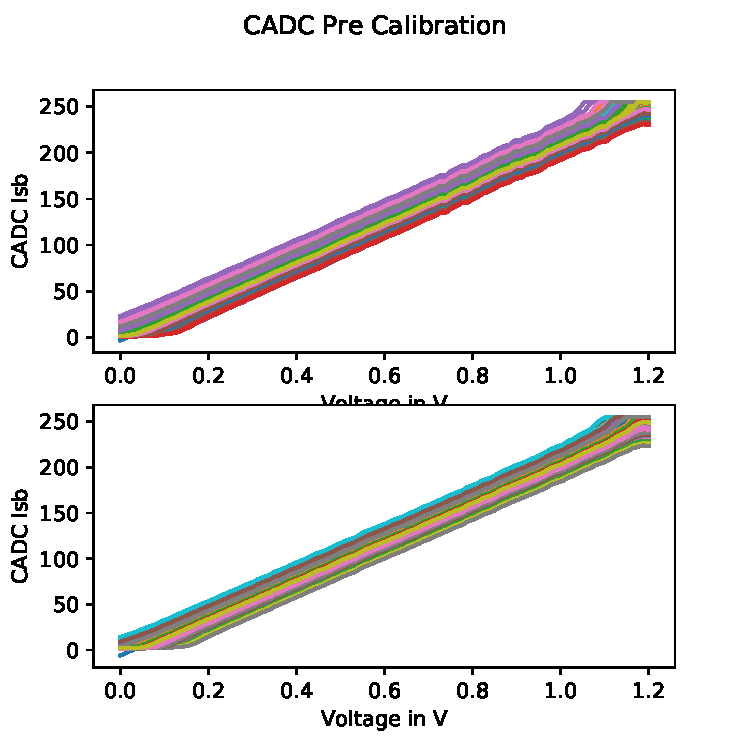
\includegraphics[width=\textwidth]{figures/temporary/cadc_pre_calib_hx70.pdf}
		\label{precadccalib}
	\end{subfigure}
	\begin{subfigure}{0.5\textwidth}
		\caption{}
		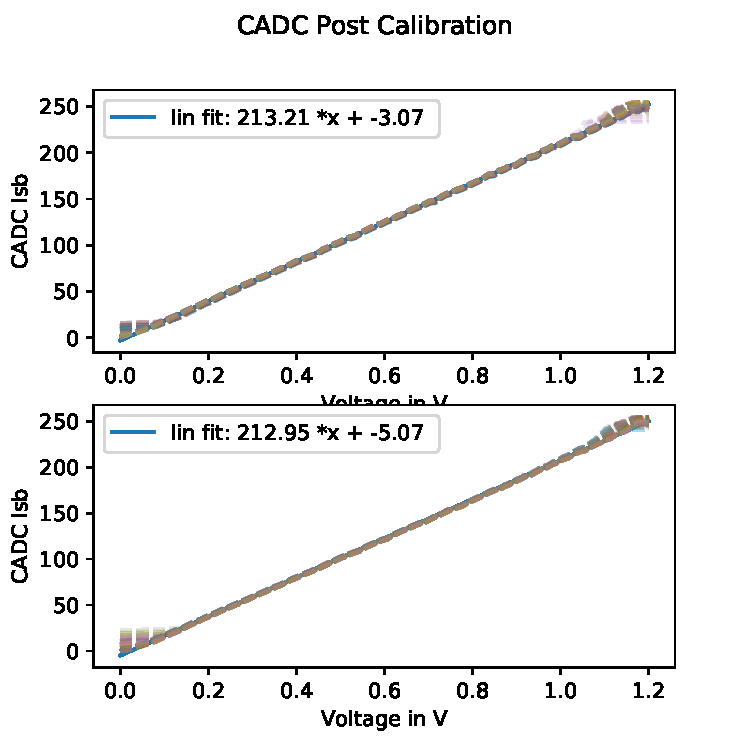
\includegraphics[width=\textwidth]{figures/temporary/cadc_post_calib_hx70.pdf}
		\label{postcadccalib}
	\end{subfigure}
	\caption[Pre and post calibration state of the \gls{cadc}]{Pre and post calibration state of the \gls{cadc}. (\subref{precadccalib}) The raw cadc data of an controlled voltage ranging from 0 to \SI{1.2}{\V}. (\subref{postcadccalib}) the cadc parameters are manually adjusted, such that they cover a useful dynamic range. The offset per channel can then be easily computed and corrected. The manual method was preferred over an automated fit-routine, since the ramp and slope parameters showed a sensitive cross-dependency in certain areas.}
	\label{cadccalibration}
\end{figure}

For the use-case of the \gls{cadc} readout during the experiment, it is vital that both the measured trace and the recorded spike times by the digital back end are synchronized. The result of a respective offset measurement yields an offset of $\delta t \approx \SI{2.2}{\milli \s}$.

\subsubsection*{Calibration of \gls{lif} Neuron}
The new chip revision did not yet get rid of the imperfection the come with analog neuromorphic hardware. Despite the self-correcting behavior of learning algorithms, the chip requires at least some calibrating before the experiment can be executed.

At the time of the experiment, the development of chip-specific software for the new prototype was in an early stage. Among others, there was a lack of a calibration database and more generally, a lack of available calibrated hardware resources. This was largely due to an at that time slow and static calibration routine, that required the allocation of human and hardware resources for several hours to tune a setup.

The efficient parallelized readout of the \gls{cadc} presented itself to be a viable basis to put a quick alternative calibration routine into action. The main objective of the new routine is to provide a fast calibration that requires little interaction to bring a setup into a usable state with respect to the specific experiment requirements. 

Similar to the circles task, the binary search algorithm is chosen to find the proper \gls{dac} values of the analog parameters. Moreover, only a subset of the available parameters is tuned, namely the potentials of the \gls{lif} model \gls{v_leak}, \gls{v_reset} and \gls{thres}. By design, the potentials of the synaptic input $V_\text{syn, inh}$ and $V_\text{syn, exc}$ have a cross-dependency to the resting potential and thus need to be considered as well. The temporal constants \gls{tau_m} and \gls{tau_syn} are certainly important parameters in the \gls{lif} model, but the induced error by their misalignment is, at least for the chosen task, not heavily hampering the performance.

At the beginning, the calibration appeared to not work properly. A known issue is the cross talk between individual capacitive parameter memory cells, that arises if several cells are set to same value. By the design of the binary search algorithm, this event occurs repeatedly making the binary search a suboptimal choice for the calibration of the new chip. The development of a proper gradient based calibration has already been started, but for the use case in this experiment the existing code base could be sufficiently stabilized with two minor adaptations. First, a random variation is consequently applied to all ``unused" \gls{dac}-values and second, the binary search algorithm is extended with a fall back option of the best parameter setting so far. The results of the final calibration for the \gls{lif} parameters are shown in \cref{hxprepostcalib}.
\begin{figure}
	\begin{subfigure}{0.32\textwidth}
		\caption{}
		\centering
		%% Creator: Matplotlib, PGF backend
%%
%% To include the figure in your LaTeX document, write
%%   \input{<filename>.pgf}
%%
%% Make sure the required packages are loaded in your preamble
%%   \usepackage{pgf}
%%
%% Figures using additional raster images can only be included by \input if
%% they are in the same directory as the main LaTeX file. For loading figures
%% from other directories you can use the `import` package
%%   \usepackage{import}
%% and then include the figures with
%%   \import{<path to file>}{<filename>.pgf}
%%
%% Matplotlib used the following preamble
%%   \usepackage{amsmath} \usepackage{pifont} \usepackage{xcolor} \definecolor{green}{HTML}{467821} \definecolor{red}{HTML}{CF4457} \usepackage[detect-all]{siunitx}
%%   \usepackage{fontspec}
%%
\begingroup%
\makeatletter%
\begin{pgfpicture}%
\pgfpathrectangle{\pgfpointorigin}{\pgfqpoint{2.105974in}{2.023578in}}%
\pgfusepath{use as bounding box, clip}%
\begin{pgfscope}%
\pgfsetbuttcap%
\pgfsetmiterjoin%
\pgfsetlinewidth{0.000000pt}%
\definecolor{currentstroke}{rgb}{0.000000,0.000000,0.000000}%
\pgfsetstrokecolor{currentstroke}%
\pgfsetstrokeopacity{0.000000}%
\pgfsetdash{}{0pt}%
\pgfpathmoveto{\pgfqpoint{0.000000in}{0.000000in}}%
\pgfpathlineto{\pgfqpoint{2.105974in}{0.000000in}}%
\pgfpathlineto{\pgfqpoint{2.105974in}{2.023578in}}%
\pgfpathlineto{\pgfqpoint{0.000000in}{2.023578in}}%
\pgfpathclose%
\pgfusepath{}%
\end{pgfscope}%
\begin{pgfscope}%
\pgfsetbuttcap%
\pgfsetmiterjoin%
\pgfsetlinewidth{0.000000pt}%
\definecolor{currentstroke}{rgb}{0.000000,0.000000,0.000000}%
\pgfsetstrokecolor{currentstroke}%
\pgfsetstrokeopacity{0.000000}%
\pgfsetdash{}{0pt}%
\pgfpathmoveto{\pgfqpoint{0.384118in}{0.383578in}}%
\pgfpathlineto{\pgfqpoint{1.934118in}{0.383578in}}%
\pgfpathlineto{\pgfqpoint{1.934118in}{1.923578in}}%
\pgfpathlineto{\pgfqpoint{0.384118in}{1.923578in}}%
\pgfpathclose%
\pgfusepath{}%
\end{pgfscope}%
\begin{pgfscope}%
\pgfsetbuttcap%
\pgfsetroundjoin%
\definecolor{currentfill}{rgb}{0.317647,0.317647,0.317647}%
\pgfsetfillcolor{currentfill}%
\pgfsetlinewidth{0.501875pt}%
\definecolor{currentstroke}{rgb}{0.317647,0.317647,0.317647}%
\pgfsetstrokecolor{currentstroke}%
\pgfsetdash{}{0pt}%
\pgfsys@defobject{currentmarker}{\pgfqpoint{0.000000in}{-0.020833in}}{\pgfqpoint{0.000000in}{0.000000in}}{%
\pgfpathmoveto{\pgfqpoint{0.000000in}{0.000000in}}%
\pgfpathlineto{\pgfqpoint{0.000000in}{-0.020833in}}%
\pgfusepath{stroke,fill}%
}%
\begin{pgfscope}%
\pgfsys@transformshift{0.605547in}{0.383578in}%
\pgfsys@useobject{currentmarker}{}%
\end{pgfscope}%
\end{pgfscope}%
\begin{pgfscope}%
\definecolor{textcolor}{rgb}{0.317647,0.317647,0.317647}%
\pgfsetstrokecolor{textcolor}%
\pgfsetfillcolor{textcolor}%
\pgftext[x=0.605547in,y=0.334967in,,top]{\color{textcolor}\rmfamily\fontsize{6.664000}{7.996800}\selectfont \(\displaystyle 0.4\)}%
\end{pgfscope}%
\begin{pgfscope}%
\pgfsetbuttcap%
\pgfsetroundjoin%
\definecolor{currentfill}{rgb}{0.317647,0.317647,0.317647}%
\pgfsetfillcolor{currentfill}%
\pgfsetlinewidth{0.501875pt}%
\definecolor{currentstroke}{rgb}{0.317647,0.317647,0.317647}%
\pgfsetstrokecolor{currentstroke}%
\pgfsetdash{}{0pt}%
\pgfsys@defobject{currentmarker}{\pgfqpoint{0.000000in}{-0.020833in}}{\pgfqpoint{0.000000in}{0.000000in}}{%
\pgfpathmoveto{\pgfqpoint{0.000000in}{0.000000in}}%
\pgfpathlineto{\pgfqpoint{0.000000in}{-0.020833in}}%
\pgfusepath{stroke,fill}%
}%
\begin{pgfscope}%
\pgfsys@transformshift{1.048404in}{0.383578in}%
\pgfsys@useobject{currentmarker}{}%
\end{pgfscope}%
\end{pgfscope}%
\begin{pgfscope}%
\definecolor{textcolor}{rgb}{0.317647,0.317647,0.317647}%
\pgfsetstrokecolor{textcolor}%
\pgfsetfillcolor{textcolor}%
\pgftext[x=1.048404in,y=0.334967in,,top]{\color{textcolor}\rmfamily\fontsize{6.664000}{7.996800}\selectfont \(\displaystyle 0.5\)}%
\end{pgfscope}%
\begin{pgfscope}%
\pgfsetbuttcap%
\pgfsetroundjoin%
\definecolor{currentfill}{rgb}{0.317647,0.317647,0.317647}%
\pgfsetfillcolor{currentfill}%
\pgfsetlinewidth{0.501875pt}%
\definecolor{currentstroke}{rgb}{0.317647,0.317647,0.317647}%
\pgfsetstrokecolor{currentstroke}%
\pgfsetdash{}{0pt}%
\pgfsys@defobject{currentmarker}{\pgfqpoint{0.000000in}{-0.020833in}}{\pgfqpoint{0.000000in}{0.000000in}}{%
\pgfpathmoveto{\pgfqpoint{0.000000in}{0.000000in}}%
\pgfpathlineto{\pgfqpoint{0.000000in}{-0.020833in}}%
\pgfusepath{stroke,fill}%
}%
\begin{pgfscope}%
\pgfsys@transformshift{1.491261in}{0.383578in}%
\pgfsys@useobject{currentmarker}{}%
\end{pgfscope}%
\end{pgfscope}%
\begin{pgfscope}%
\definecolor{textcolor}{rgb}{0.317647,0.317647,0.317647}%
\pgfsetstrokecolor{textcolor}%
\pgfsetfillcolor{textcolor}%
\pgftext[x=1.491261in,y=0.334967in,,top]{\color{textcolor}\rmfamily\fontsize{6.664000}{7.996800}\selectfont \(\displaystyle 0.6\)}%
\end{pgfscope}%
\begin{pgfscope}%
\pgfsetbuttcap%
\pgfsetroundjoin%
\definecolor{currentfill}{rgb}{0.317647,0.317647,0.317647}%
\pgfsetfillcolor{currentfill}%
\pgfsetlinewidth{0.501875pt}%
\definecolor{currentstroke}{rgb}{0.317647,0.317647,0.317647}%
\pgfsetstrokecolor{currentstroke}%
\pgfsetdash{}{0pt}%
\pgfsys@defobject{currentmarker}{\pgfqpoint{0.000000in}{-0.020833in}}{\pgfqpoint{0.000000in}{0.000000in}}{%
\pgfpathmoveto{\pgfqpoint{0.000000in}{0.000000in}}%
\pgfpathlineto{\pgfqpoint{0.000000in}{-0.020833in}}%
\pgfusepath{stroke,fill}%
}%
\begin{pgfscope}%
\pgfsys@transformshift{1.934118in}{0.383578in}%
\pgfsys@useobject{currentmarker}{}%
\end{pgfscope}%
\end{pgfscope}%
\begin{pgfscope}%
\definecolor{textcolor}{rgb}{0.317647,0.317647,0.317647}%
\pgfsetstrokecolor{textcolor}%
\pgfsetfillcolor{textcolor}%
\pgftext[x=1.934118in,y=0.334967in,,top]{\color{textcolor}\rmfamily\fontsize{6.664000}{7.996800}\selectfont \(\displaystyle 0.7\)}%
\end{pgfscope}%
\begin{pgfscope}%
\definecolor{textcolor}{rgb}{0.317647,0.317647,0.317647}%
\pgfsetstrokecolor{textcolor}%
\pgfsetfillcolor{textcolor}%
\pgftext[x=1.159118in,y=0.197222in,,top]{\color{textcolor}\rmfamily\fontsize{6.664000}{7.996800}\selectfont \(\displaystyle V_\mathrm{leak} \quad (\si{\V})\)}%
\end{pgfscope}%
\begin{pgfscope}%
\pgfsetbuttcap%
\pgfsetroundjoin%
\definecolor{currentfill}{rgb}{0.317647,0.317647,0.317647}%
\pgfsetfillcolor{currentfill}%
\pgfsetlinewidth{0.501875pt}%
\definecolor{currentstroke}{rgb}{0.317647,0.317647,0.317647}%
\pgfsetstrokecolor{currentstroke}%
\pgfsetdash{}{0pt}%
\pgfsys@defobject{currentmarker}{\pgfqpoint{-0.020833in}{0.000000in}}{\pgfqpoint{0.000000in}{0.000000in}}{%
\pgfpathmoveto{\pgfqpoint{0.000000in}{0.000000in}}%
\pgfpathlineto{\pgfqpoint{-0.020833in}{0.000000in}}%
\pgfusepath{stroke,fill}%
}%
\begin{pgfscope}%
\pgfsys@transformshift{0.384118in}{0.383578in}%
\pgfsys@useobject{currentmarker}{}%
\end{pgfscope}%
\end{pgfscope}%
\begin{pgfscope}%
\definecolor{textcolor}{rgb}{0.317647,0.317647,0.317647}%
\pgfsetstrokecolor{textcolor}%
\pgfsetfillcolor{textcolor}%
\pgftext[x=0.294033in,y=0.351461in,left,base]{\color{textcolor}\rmfamily\fontsize{6.664000}{7.996800}\selectfont \(\displaystyle 0\)}%
\end{pgfscope}%
\begin{pgfscope}%
\pgfsetbuttcap%
\pgfsetroundjoin%
\definecolor{currentfill}{rgb}{0.317647,0.317647,0.317647}%
\pgfsetfillcolor{currentfill}%
\pgfsetlinewidth{0.501875pt}%
\definecolor{currentstroke}{rgb}{0.317647,0.317647,0.317647}%
\pgfsetstrokecolor{currentstroke}%
\pgfsetdash{}{0pt}%
\pgfsys@defobject{currentmarker}{\pgfqpoint{-0.020833in}{0.000000in}}{\pgfqpoint{0.000000in}{0.000000in}}{%
\pgfpathmoveto{\pgfqpoint{0.000000in}{0.000000in}}%
\pgfpathlineto{\pgfqpoint{-0.020833in}{0.000000in}}%
\pgfusepath{stroke,fill}%
}%
\begin{pgfscope}%
\pgfsys@transformshift{0.384118in}{0.660102in}%
\pgfsys@useobject{currentmarker}{}%
\end{pgfscope}%
\end{pgfscope}%
\begin{pgfscope}%
\definecolor{textcolor}{rgb}{0.317647,0.317647,0.317647}%
\pgfsetstrokecolor{textcolor}%
\pgfsetfillcolor{textcolor}%
\pgftext[x=0.238670in,y=0.627985in,left,base]{\color{textcolor}\rmfamily\fontsize{6.664000}{7.996800}\selectfont \(\displaystyle 10\)}%
\end{pgfscope}%
\begin{pgfscope}%
\pgfsetbuttcap%
\pgfsetroundjoin%
\definecolor{currentfill}{rgb}{0.317647,0.317647,0.317647}%
\pgfsetfillcolor{currentfill}%
\pgfsetlinewidth{0.501875pt}%
\definecolor{currentstroke}{rgb}{0.317647,0.317647,0.317647}%
\pgfsetstrokecolor{currentstroke}%
\pgfsetdash{}{0pt}%
\pgfsys@defobject{currentmarker}{\pgfqpoint{-0.020833in}{0.000000in}}{\pgfqpoint{0.000000in}{0.000000in}}{%
\pgfpathmoveto{\pgfqpoint{0.000000in}{0.000000in}}%
\pgfpathlineto{\pgfqpoint{-0.020833in}{0.000000in}}%
\pgfusepath{stroke,fill}%
}%
\begin{pgfscope}%
\pgfsys@transformshift{0.384118in}{0.936625in}%
\pgfsys@useobject{currentmarker}{}%
\end{pgfscope}%
\end{pgfscope}%
\begin{pgfscope}%
\definecolor{textcolor}{rgb}{0.317647,0.317647,0.317647}%
\pgfsetstrokecolor{textcolor}%
\pgfsetfillcolor{textcolor}%
\pgftext[x=0.238670in,y=0.904508in,left,base]{\color{textcolor}\rmfamily\fontsize{6.664000}{7.996800}\selectfont \(\displaystyle 20\)}%
\end{pgfscope}%
\begin{pgfscope}%
\pgfsetbuttcap%
\pgfsetroundjoin%
\definecolor{currentfill}{rgb}{0.317647,0.317647,0.317647}%
\pgfsetfillcolor{currentfill}%
\pgfsetlinewidth{0.501875pt}%
\definecolor{currentstroke}{rgb}{0.317647,0.317647,0.317647}%
\pgfsetstrokecolor{currentstroke}%
\pgfsetdash{}{0pt}%
\pgfsys@defobject{currentmarker}{\pgfqpoint{-0.020833in}{0.000000in}}{\pgfqpoint{0.000000in}{0.000000in}}{%
\pgfpathmoveto{\pgfqpoint{0.000000in}{0.000000in}}%
\pgfpathlineto{\pgfqpoint{-0.020833in}{0.000000in}}%
\pgfusepath{stroke,fill}%
}%
\begin{pgfscope}%
\pgfsys@transformshift{0.384118in}{1.213149in}%
\pgfsys@useobject{currentmarker}{}%
\end{pgfscope}%
\end{pgfscope}%
\begin{pgfscope}%
\definecolor{textcolor}{rgb}{0.317647,0.317647,0.317647}%
\pgfsetstrokecolor{textcolor}%
\pgfsetfillcolor{textcolor}%
\pgftext[x=0.238670in,y=1.181032in,left,base]{\color{textcolor}\rmfamily\fontsize{6.664000}{7.996800}\selectfont \(\displaystyle 30\)}%
\end{pgfscope}%
\begin{pgfscope}%
\pgfsetbuttcap%
\pgfsetroundjoin%
\definecolor{currentfill}{rgb}{0.317647,0.317647,0.317647}%
\pgfsetfillcolor{currentfill}%
\pgfsetlinewidth{0.501875pt}%
\definecolor{currentstroke}{rgb}{0.317647,0.317647,0.317647}%
\pgfsetstrokecolor{currentstroke}%
\pgfsetdash{}{0pt}%
\pgfsys@defobject{currentmarker}{\pgfqpoint{-0.020833in}{0.000000in}}{\pgfqpoint{0.000000in}{0.000000in}}{%
\pgfpathmoveto{\pgfqpoint{0.000000in}{0.000000in}}%
\pgfpathlineto{\pgfqpoint{-0.020833in}{0.000000in}}%
\pgfusepath{stroke,fill}%
}%
\begin{pgfscope}%
\pgfsys@transformshift{0.384118in}{1.489672in}%
\pgfsys@useobject{currentmarker}{}%
\end{pgfscope}%
\end{pgfscope}%
\begin{pgfscope}%
\definecolor{textcolor}{rgb}{0.317647,0.317647,0.317647}%
\pgfsetstrokecolor{textcolor}%
\pgfsetfillcolor{textcolor}%
\pgftext[x=0.238670in,y=1.457556in,left,base]{\color{textcolor}\rmfamily\fontsize{6.664000}{7.996800}\selectfont \(\displaystyle 40\)}%
\end{pgfscope}%
\begin{pgfscope}%
\pgfsetbuttcap%
\pgfsetroundjoin%
\definecolor{currentfill}{rgb}{0.317647,0.317647,0.317647}%
\pgfsetfillcolor{currentfill}%
\pgfsetlinewidth{0.501875pt}%
\definecolor{currentstroke}{rgb}{0.317647,0.317647,0.317647}%
\pgfsetstrokecolor{currentstroke}%
\pgfsetdash{}{0pt}%
\pgfsys@defobject{currentmarker}{\pgfqpoint{-0.020833in}{0.000000in}}{\pgfqpoint{0.000000in}{0.000000in}}{%
\pgfpathmoveto{\pgfqpoint{0.000000in}{0.000000in}}%
\pgfpathlineto{\pgfqpoint{-0.020833in}{0.000000in}}%
\pgfusepath{stroke,fill}%
}%
\begin{pgfscope}%
\pgfsys@transformshift{0.384118in}{1.766196in}%
\pgfsys@useobject{currentmarker}{}%
\end{pgfscope}%
\end{pgfscope}%
\begin{pgfscope}%
\definecolor{textcolor}{rgb}{0.317647,0.317647,0.317647}%
\pgfsetstrokecolor{textcolor}%
\pgfsetfillcolor{textcolor}%
\pgftext[x=0.238670in,y=1.734079in,left,base]{\color{textcolor}\rmfamily\fontsize{6.664000}{7.996800}\selectfont \(\displaystyle 50\)}%
\end{pgfscope}%
\begin{pgfscope}%
\definecolor{textcolor}{rgb}{0.317647,0.317647,0.317647}%
\pgfsetstrokecolor{textcolor}%
\pgfsetfillcolor{textcolor}%
\pgftext[x=0.183115in,y=1.153578in,,bottom,rotate=90.000000]{\color{textcolor}\rmfamily\fontsize{6.664000}{7.996800}\selectfont density}%
\end{pgfscope}%
\begin{pgfscope}%
\pgfpathrectangle{\pgfqpoint{0.384118in}{0.383578in}}{\pgfqpoint{1.550000in}{1.540000in}}%
\pgfusepath{clip}%
\pgfsetbuttcap%
\pgfsetmiterjoin%
\definecolor{currentfill}{rgb}{0.333333,0.333333,0.333333}%
\pgfsetfillcolor{currentfill}%
\pgfsetfillopacity{0.400000}%
\pgfsetlinewidth{0.000000pt}%
\definecolor{currentstroke}{rgb}{0.000000,0.000000,0.000000}%
\pgfsetstrokecolor{currentstroke}%
\pgfsetstrokeopacity{0.400000}%
\pgfsetdash{}{0pt}%
\pgfpathmoveto{\pgfqpoint{0.489761in}{0.383578in}}%
\pgfpathlineto{\pgfqpoint{0.676907in}{0.383578in}}%
\pgfpathlineto{\pgfqpoint{0.676907in}{0.460260in}}%
\pgfpathlineto{\pgfqpoint{0.489761in}{0.460260in}}%
\pgfpathclose%
\pgfusepath{fill}%
\end{pgfscope}%
\begin{pgfscope}%
\pgfpathrectangle{\pgfqpoint{0.384118in}{0.383578in}}{\pgfqpoint{1.550000in}{1.540000in}}%
\pgfusepath{clip}%
\pgfsetbuttcap%
\pgfsetmiterjoin%
\definecolor{currentfill}{rgb}{0.333333,0.333333,0.333333}%
\pgfsetfillcolor{currentfill}%
\pgfsetfillopacity{0.400000}%
\pgfsetlinewidth{0.000000pt}%
\definecolor{currentstroke}{rgb}{0.000000,0.000000,0.000000}%
\pgfsetstrokecolor{currentstroke}%
\pgfsetstrokeopacity{0.400000}%
\pgfsetdash{}{0pt}%
\pgfpathmoveto{\pgfqpoint{0.676907in}{0.383578in}}%
\pgfpathlineto{\pgfqpoint{0.864054in}{0.383578in}}%
\pgfpathlineto{\pgfqpoint{0.864054in}{0.490933in}}%
\pgfpathlineto{\pgfqpoint{0.676907in}{0.490933in}}%
\pgfpathclose%
\pgfusepath{fill}%
\end{pgfscope}%
\begin{pgfscope}%
\pgfpathrectangle{\pgfqpoint{0.384118in}{0.383578in}}{\pgfqpoint{1.550000in}{1.540000in}}%
\pgfusepath{clip}%
\pgfsetbuttcap%
\pgfsetmiterjoin%
\definecolor{currentfill}{rgb}{0.333333,0.333333,0.333333}%
\pgfsetfillcolor{currentfill}%
\pgfsetfillopacity{0.400000}%
\pgfsetlinewidth{0.000000pt}%
\definecolor{currentstroke}{rgb}{0.000000,0.000000,0.000000}%
\pgfsetstrokecolor{currentstroke}%
\pgfsetstrokeopacity{0.400000}%
\pgfsetdash{}{0pt}%
\pgfpathmoveto{\pgfqpoint{0.864054in}{0.383578in}}%
\pgfpathlineto{\pgfqpoint{1.051200in}{0.383578in}}%
\pgfpathlineto{\pgfqpoint{1.051200in}{0.490933in}}%
\pgfpathlineto{\pgfqpoint{0.864054in}{0.490933in}}%
\pgfpathclose%
\pgfusepath{fill}%
\end{pgfscope}%
\begin{pgfscope}%
\pgfpathrectangle{\pgfqpoint{0.384118in}{0.383578in}}{\pgfqpoint{1.550000in}{1.540000in}}%
\pgfusepath{clip}%
\pgfsetbuttcap%
\pgfsetmiterjoin%
\definecolor{currentfill}{rgb}{0.333333,0.333333,0.333333}%
\pgfsetfillcolor{currentfill}%
\pgfsetfillopacity{0.400000}%
\pgfsetlinewidth{0.000000pt}%
\definecolor{currentstroke}{rgb}{0.000000,0.000000,0.000000}%
\pgfsetstrokecolor{currentstroke}%
\pgfsetstrokeopacity{0.400000}%
\pgfsetdash{}{0pt}%
\pgfpathmoveto{\pgfqpoint{1.051200in}{0.383578in}}%
\pgfpathlineto{\pgfqpoint{1.238347in}{0.383578in}}%
\pgfpathlineto{\pgfqpoint{1.238347in}{0.536943in}}%
\pgfpathlineto{\pgfqpoint{1.051200in}{0.536943in}}%
\pgfpathclose%
\pgfusepath{fill}%
\end{pgfscope}%
\begin{pgfscope}%
\pgfpathrectangle{\pgfqpoint{0.384118in}{0.383578in}}{\pgfqpoint{1.550000in}{1.540000in}}%
\pgfusepath{clip}%
\pgfsetbuttcap%
\pgfsetmiterjoin%
\definecolor{currentfill}{rgb}{0.333333,0.333333,0.333333}%
\pgfsetfillcolor{currentfill}%
\pgfsetfillopacity{0.400000}%
\pgfsetlinewidth{0.000000pt}%
\definecolor{currentstroke}{rgb}{0.000000,0.000000,0.000000}%
\pgfsetstrokecolor{currentstroke}%
\pgfsetstrokeopacity{0.400000}%
\pgfsetdash{}{0pt}%
\pgfpathmoveto{\pgfqpoint{1.238347in}{0.383578in}}%
\pgfpathlineto{\pgfqpoint{1.425493in}{0.383578in}}%
\pgfpathlineto{\pgfqpoint{1.425493in}{0.475597in}}%
\pgfpathlineto{\pgfqpoint{1.238347in}{0.475597in}}%
\pgfpathclose%
\pgfusepath{fill}%
\end{pgfscope}%
\begin{pgfscope}%
\pgfpathrectangle{\pgfqpoint{0.384118in}{0.383578in}}{\pgfqpoint{1.550000in}{1.540000in}}%
\pgfusepath{clip}%
\pgfsetbuttcap%
\pgfsetmiterjoin%
\definecolor{currentfill}{rgb}{0.333333,0.333333,0.333333}%
\pgfsetfillcolor{currentfill}%
\pgfsetfillopacity{0.400000}%
\pgfsetlinewidth{0.000000pt}%
\definecolor{currentstroke}{rgb}{0.000000,0.000000,0.000000}%
\pgfsetstrokecolor{currentstroke}%
\pgfsetstrokeopacity{0.400000}%
\pgfsetdash{}{0pt}%
\pgfpathmoveto{\pgfqpoint{1.425493in}{0.383578in}}%
\pgfpathlineto{\pgfqpoint{1.612640in}{0.383578in}}%
\pgfpathlineto{\pgfqpoint{1.612640in}{0.465373in}}%
\pgfpathlineto{\pgfqpoint{1.425493in}{0.465373in}}%
\pgfpathclose%
\pgfusepath{fill}%
\end{pgfscope}%
\begin{pgfscope}%
\pgfpathrectangle{\pgfqpoint{0.384118in}{0.383578in}}{\pgfqpoint{1.550000in}{1.540000in}}%
\pgfusepath{clip}%
\pgfsetbuttcap%
\pgfsetmiterjoin%
\definecolor{currentfill}{rgb}{0.333333,0.333333,0.333333}%
\pgfsetfillcolor{currentfill}%
\pgfsetfillopacity{0.400000}%
\pgfsetlinewidth{0.000000pt}%
\definecolor{currentstroke}{rgb}{0.000000,0.000000,0.000000}%
\pgfsetstrokecolor{currentstroke}%
\pgfsetstrokeopacity{0.400000}%
\pgfsetdash{}{0pt}%
\pgfpathmoveto{\pgfqpoint{1.612640in}{0.383578in}}%
\pgfpathlineto{\pgfqpoint{1.799787in}{0.383578in}}%
\pgfpathlineto{\pgfqpoint{1.799787in}{0.419363in}}%
\pgfpathlineto{\pgfqpoint{1.612640in}{0.419363in}}%
\pgfpathclose%
\pgfusepath{fill}%
\end{pgfscope}%
\begin{pgfscope}%
\pgfpathrectangle{\pgfqpoint{0.384118in}{0.383578in}}{\pgfqpoint{1.550000in}{1.540000in}}%
\pgfusepath{clip}%
\pgfsetbuttcap%
\pgfsetmiterjoin%
\definecolor{currentfill}{rgb}{0.686275,0.352941,0.313725}%
\pgfsetfillcolor{currentfill}%
\pgfsetfillopacity{0.400000}%
\pgfsetlinewidth{0.000000pt}%
\definecolor{currentstroke}{rgb}{0.000000,0.000000,0.000000}%
\pgfsetstrokecolor{currentstroke}%
\pgfsetstrokeopacity{0.400000}%
\pgfsetdash{}{0pt}%
\pgfpathmoveto{\pgfqpoint{0.951037in}{0.383578in}}%
\pgfpathlineto{\pgfqpoint{0.972564in}{0.383578in}}%
\pgfpathlineto{\pgfqpoint{0.972564in}{0.472467in}}%
\pgfpathlineto{\pgfqpoint{0.951037in}{0.472467in}}%
\pgfpathclose%
\pgfusepath{fill}%
\end{pgfscope}%
\begin{pgfscope}%
\pgfpathrectangle{\pgfqpoint{0.384118in}{0.383578in}}{\pgfqpoint{1.550000in}{1.540000in}}%
\pgfusepath{clip}%
\pgfsetbuttcap%
\pgfsetmiterjoin%
\definecolor{currentfill}{rgb}{0.686275,0.352941,0.313725}%
\pgfsetfillcolor{currentfill}%
\pgfsetfillopacity{0.400000}%
\pgfsetlinewidth{0.000000pt}%
\definecolor{currentstroke}{rgb}{0.000000,0.000000,0.000000}%
\pgfsetstrokecolor{currentstroke}%
\pgfsetstrokeopacity{0.400000}%
\pgfsetdash{}{0pt}%
\pgfpathmoveto{\pgfqpoint{0.972564in}{0.383578in}}%
\pgfpathlineto{\pgfqpoint{0.994090in}{0.383578in}}%
\pgfpathlineto{\pgfqpoint{0.994090in}{0.516911in}}%
\pgfpathlineto{\pgfqpoint{0.972564in}{0.516911in}}%
\pgfpathclose%
\pgfusepath{fill}%
\end{pgfscope}%
\begin{pgfscope}%
\pgfpathrectangle{\pgfqpoint{0.384118in}{0.383578in}}{\pgfqpoint{1.550000in}{1.540000in}}%
\pgfusepath{clip}%
\pgfsetbuttcap%
\pgfsetmiterjoin%
\definecolor{currentfill}{rgb}{0.686275,0.352941,0.313725}%
\pgfsetfillcolor{currentfill}%
\pgfsetfillopacity{0.400000}%
\pgfsetlinewidth{0.000000pt}%
\definecolor{currentstroke}{rgb}{0.000000,0.000000,0.000000}%
\pgfsetstrokecolor{currentstroke}%
\pgfsetstrokeopacity{0.400000}%
\pgfsetdash{}{0pt}%
\pgfpathmoveto{\pgfqpoint{0.994090in}{0.383578in}}%
\pgfpathlineto{\pgfqpoint{1.015616in}{0.383578in}}%
\pgfpathlineto{\pgfqpoint{1.015616in}{0.961356in}}%
\pgfpathlineto{\pgfqpoint{0.994090in}{0.961356in}}%
\pgfpathclose%
\pgfusepath{fill}%
\end{pgfscope}%
\begin{pgfscope}%
\pgfpathrectangle{\pgfqpoint{0.384118in}{0.383578in}}{\pgfqpoint{1.550000in}{1.540000in}}%
\pgfusepath{clip}%
\pgfsetbuttcap%
\pgfsetmiterjoin%
\definecolor{currentfill}{rgb}{0.686275,0.352941,0.313725}%
\pgfsetfillcolor{currentfill}%
\pgfsetfillopacity{0.400000}%
\pgfsetlinewidth{0.000000pt}%
\definecolor{currentstroke}{rgb}{0.000000,0.000000,0.000000}%
\pgfsetstrokecolor{currentstroke}%
\pgfsetstrokeopacity{0.400000}%
\pgfsetdash{}{0pt}%
\pgfpathmoveto{\pgfqpoint{1.015616in}{0.383578in}}%
\pgfpathlineto{\pgfqpoint{1.037142in}{0.383578in}}%
\pgfpathlineto{\pgfqpoint{1.037142in}{1.228022in}}%
\pgfpathlineto{\pgfqpoint{1.015616in}{1.228022in}}%
\pgfpathclose%
\pgfusepath{fill}%
\end{pgfscope}%
\begin{pgfscope}%
\pgfpathrectangle{\pgfqpoint{0.384118in}{0.383578in}}{\pgfqpoint{1.550000in}{1.540000in}}%
\pgfusepath{clip}%
\pgfsetbuttcap%
\pgfsetmiterjoin%
\definecolor{currentfill}{rgb}{0.686275,0.352941,0.313725}%
\pgfsetfillcolor{currentfill}%
\pgfsetfillopacity{0.400000}%
\pgfsetlinewidth{0.000000pt}%
\definecolor{currentstroke}{rgb}{0.000000,0.000000,0.000000}%
\pgfsetstrokecolor{currentstroke}%
\pgfsetstrokeopacity{0.400000}%
\pgfsetdash{}{0pt}%
\pgfpathmoveto{\pgfqpoint{1.037142in}{0.383578in}}%
\pgfpathlineto{\pgfqpoint{1.058669in}{0.383578in}}%
\pgfpathlineto{\pgfqpoint{1.058669in}{1.361356in}}%
\pgfpathlineto{\pgfqpoint{1.037142in}{1.361356in}}%
\pgfpathclose%
\pgfusepath{fill}%
\end{pgfscope}%
\begin{pgfscope}%
\pgfpathrectangle{\pgfqpoint{0.384118in}{0.383578in}}{\pgfqpoint{1.550000in}{1.540000in}}%
\pgfusepath{clip}%
\pgfsetbuttcap%
\pgfsetmiterjoin%
\definecolor{currentfill}{rgb}{0.686275,0.352941,0.313725}%
\pgfsetfillcolor{currentfill}%
\pgfsetfillopacity{0.400000}%
\pgfsetlinewidth{0.000000pt}%
\definecolor{currentstroke}{rgb}{0.000000,0.000000,0.000000}%
\pgfsetstrokecolor{currentstroke}%
\pgfsetstrokeopacity{0.400000}%
\pgfsetdash{}{0pt}%
\pgfpathmoveto{\pgfqpoint{1.058669in}{0.383578in}}%
\pgfpathlineto{\pgfqpoint{1.080195in}{0.383578in}}%
\pgfpathlineto{\pgfqpoint{1.080195in}{1.850245in}}%
\pgfpathlineto{\pgfqpoint{1.058669in}{1.850245in}}%
\pgfpathclose%
\pgfusepath{fill}%
\end{pgfscope}%
\begin{pgfscope}%
\pgfpathrectangle{\pgfqpoint{0.384118in}{0.383578in}}{\pgfqpoint{1.550000in}{1.540000in}}%
\pgfusepath{clip}%
\pgfsetbuttcap%
\pgfsetmiterjoin%
\definecolor{currentfill}{rgb}{0.686275,0.352941,0.313725}%
\pgfsetfillcolor{currentfill}%
\pgfsetfillopacity{0.400000}%
\pgfsetlinewidth{0.000000pt}%
\definecolor{currentstroke}{rgb}{0.000000,0.000000,0.000000}%
\pgfsetstrokecolor{currentstroke}%
\pgfsetstrokeopacity{0.400000}%
\pgfsetdash{}{0pt}%
\pgfpathmoveto{\pgfqpoint{1.080195in}{0.383578in}}%
\pgfpathlineto{\pgfqpoint{1.101721in}{0.383578in}}%
\pgfpathlineto{\pgfqpoint{1.101721in}{1.539134in}}%
\pgfpathlineto{\pgfqpoint{1.080195in}{1.539134in}}%
\pgfpathclose%
\pgfusepath{fill}%
\end{pgfscope}%
\begin{pgfscope}%
\pgfpathrectangle{\pgfqpoint{0.384118in}{0.383578in}}{\pgfqpoint{1.550000in}{1.540000in}}%
\pgfusepath{clip}%
\pgfsetbuttcap%
\pgfsetmiterjoin%
\definecolor{currentfill}{rgb}{0.686275,0.352941,0.313725}%
\pgfsetfillcolor{currentfill}%
\pgfsetfillopacity{0.400000}%
\pgfsetlinewidth{0.000000pt}%
\definecolor{currentstroke}{rgb}{0.000000,0.000000,0.000000}%
\pgfsetstrokecolor{currentstroke}%
\pgfsetstrokeopacity{0.400000}%
\pgfsetdash{}{0pt}%
\pgfpathmoveto{\pgfqpoint{1.101721in}{0.383578in}}%
\pgfpathlineto{\pgfqpoint{1.123247in}{0.383578in}}%
\pgfpathlineto{\pgfqpoint{1.123247in}{0.561356in}}%
\pgfpathlineto{\pgfqpoint{1.101721in}{0.561356in}}%
\pgfpathclose%
\pgfusepath{fill}%
\end{pgfscope}%
\begin{pgfscope}%
\pgfpathrectangle{\pgfqpoint{0.384118in}{0.383578in}}{\pgfqpoint{1.550000in}{1.540000in}}%
\pgfusepath{clip}%
\pgfsetbuttcap%
\pgfsetmiterjoin%
\definecolor{currentfill}{rgb}{0.686275,0.352941,0.313725}%
\pgfsetfillcolor{currentfill}%
\pgfsetfillopacity{0.400000}%
\pgfsetlinewidth{0.000000pt}%
\definecolor{currentstroke}{rgb}{0.000000,0.000000,0.000000}%
\pgfsetstrokecolor{currentstroke}%
\pgfsetstrokeopacity{0.400000}%
\pgfsetdash{}{0pt}%
\pgfpathmoveto{\pgfqpoint{1.123247in}{0.383578in}}%
\pgfpathlineto{\pgfqpoint{1.144774in}{0.383578in}}%
\pgfpathlineto{\pgfqpoint{1.144774in}{0.472467in}}%
\pgfpathlineto{\pgfqpoint{1.123247in}{0.472467in}}%
\pgfpathclose%
\pgfusepath{fill}%
\end{pgfscope}%
\begin{pgfscope}%
\pgfpathrectangle{\pgfqpoint{0.384118in}{0.383578in}}{\pgfqpoint{1.550000in}{1.540000in}}%
\pgfusepath{clip}%
\pgfsetbuttcap%
\pgfsetmiterjoin%
\definecolor{currentfill}{rgb}{0.686275,0.352941,0.313725}%
\pgfsetfillcolor{currentfill}%
\pgfsetfillopacity{0.400000}%
\pgfsetlinewidth{0.000000pt}%
\definecolor{currentstroke}{rgb}{0.000000,0.000000,0.000000}%
\pgfsetstrokecolor{currentstroke}%
\pgfsetstrokeopacity{0.400000}%
\pgfsetdash{}{0pt}%
\pgfpathmoveto{\pgfqpoint{1.144774in}{0.383578in}}%
\pgfpathlineto{\pgfqpoint{1.166300in}{0.383578in}}%
\pgfpathlineto{\pgfqpoint{1.166300in}{0.472467in}}%
\pgfpathlineto{\pgfqpoint{1.144774in}{0.472467in}}%
\pgfpathclose%
\pgfusepath{fill}%
\end{pgfscope}%
\begin{pgfscope}%
\pgfpathrectangle{\pgfqpoint{0.384118in}{0.383578in}}{\pgfqpoint{1.550000in}{1.540000in}}%
\pgfusepath{clip}%
\pgfsetbuttcap%
\pgfsetmiterjoin%
\definecolor{currentfill}{rgb}{0.686275,0.352941,0.313725}%
\pgfsetfillcolor{currentfill}%
\pgfsetfillopacity{0.400000}%
\pgfsetlinewidth{0.000000pt}%
\definecolor{currentstroke}{rgb}{0.000000,0.000000,0.000000}%
\pgfsetstrokecolor{currentstroke}%
\pgfsetstrokeopacity{0.400000}%
\pgfsetdash{}{0pt}%
\pgfpathmoveto{\pgfqpoint{1.166300in}{0.383578in}}%
\pgfpathlineto{\pgfqpoint{1.187826in}{0.383578in}}%
\pgfpathlineto{\pgfqpoint{1.187826in}{0.383578in}}%
\pgfpathlineto{\pgfqpoint{1.166300in}{0.383578in}}%
\pgfpathclose%
\pgfusepath{fill}%
\end{pgfscope}%
\begin{pgfscope}%
\pgfpathrectangle{\pgfqpoint{0.384118in}{0.383578in}}{\pgfqpoint{1.550000in}{1.540000in}}%
\pgfusepath{clip}%
\pgfsetbuttcap%
\pgfsetmiterjoin%
\definecolor{currentfill}{rgb}{0.686275,0.352941,0.313725}%
\pgfsetfillcolor{currentfill}%
\pgfsetfillopacity{0.400000}%
\pgfsetlinewidth{0.000000pt}%
\definecolor{currentstroke}{rgb}{0.000000,0.000000,0.000000}%
\pgfsetstrokecolor{currentstroke}%
\pgfsetstrokeopacity{0.400000}%
\pgfsetdash{}{0pt}%
\pgfpathmoveto{\pgfqpoint{1.187826in}{0.383578in}}%
\pgfpathlineto{\pgfqpoint{1.209352in}{0.383578in}}%
\pgfpathlineto{\pgfqpoint{1.209352in}{0.472467in}}%
\pgfpathlineto{\pgfqpoint{1.187826in}{0.472467in}}%
\pgfpathclose%
\pgfusepath{fill}%
\end{pgfscope}%
\begin{pgfscope}%
\pgfpathrectangle{\pgfqpoint{0.384118in}{0.383578in}}{\pgfqpoint{1.550000in}{1.540000in}}%
\pgfusepath{clip}%
\pgfsetrectcap%
\pgfsetroundjoin%
\pgfsetlinewidth{0.803000pt}%
\definecolor{currentstroke}{rgb}{0.333333,0.333333,0.333333}%
\pgfsetstrokecolor{currentstroke}%
\pgfsetdash{}{0pt}%
\pgfpathmoveto{\pgfqpoint{0.374118in}{0.392707in}}%
\pgfpathlineto{\pgfqpoint{0.380934in}{0.393541in}}%
\pgfpathlineto{\pgfqpoint{0.401303in}{0.396580in}}%
\pgfpathlineto{\pgfqpoint{0.421672in}{0.400192in}}%
\pgfpathlineto{\pgfqpoint{0.442041in}{0.404377in}}%
\pgfpathlineto{\pgfqpoint{0.462410in}{0.409105in}}%
\pgfpathlineto{\pgfqpoint{0.482779in}{0.414315in}}%
\pgfpathlineto{\pgfqpoint{0.503148in}{0.419918in}}%
\pgfpathlineto{\pgfqpoint{0.523517in}{0.425803in}}%
\pgfpathlineto{\pgfqpoint{0.543886in}{0.431850in}}%
\pgfpathlineto{\pgfqpoint{0.564256in}{0.437936in}}%
\pgfpathlineto{\pgfqpoint{0.584625in}{0.443951in}}%
\pgfpathlineto{\pgfqpoint{0.604994in}{0.449802in}}%
\pgfpathlineto{\pgfqpoint{0.625363in}{0.455424in}}%
\pgfpathlineto{\pgfqpoint{0.645732in}{0.460777in}}%
\pgfpathlineto{\pgfqpoint{0.666101in}{0.465841in}}%
\pgfpathlineto{\pgfqpoint{0.686470in}{0.470612in}}%
\pgfpathlineto{\pgfqpoint{0.706839in}{0.475088in}}%
\pgfpathlineto{\pgfqpoint{0.727208in}{0.479264in}}%
\pgfpathlineto{\pgfqpoint{0.747577in}{0.483128in}}%
\pgfpathlineto{\pgfqpoint{0.767946in}{0.486659in}}%
\pgfpathlineto{\pgfqpoint{0.788315in}{0.489833in}}%
\pgfpathlineto{\pgfqpoint{0.808684in}{0.492631in}}%
\pgfpathlineto{\pgfqpoint{0.829053in}{0.495052in}}%
\pgfpathlineto{\pgfqpoint{0.849422in}{0.497114in}}%
\pgfpathlineto{\pgfqpoint{0.869791in}{0.498865in}}%
\pgfpathlineto{\pgfqpoint{0.890160in}{0.500377in}}%
\pgfpathlineto{\pgfqpoint{0.910529in}{0.501738in}}%
\pgfpathlineto{\pgfqpoint{0.930899in}{0.503040in}}%
\pgfpathlineto{\pgfqpoint{0.951268in}{0.504367in}}%
\pgfpathlineto{\pgfqpoint{0.971637in}{0.505774in}}%
\pgfpathlineto{\pgfqpoint{0.992006in}{0.507283in}}%
\pgfpathlineto{\pgfqpoint{1.012375in}{0.508875in}}%
\pgfpathlineto{\pgfqpoint{1.032744in}{0.510487in}}%
\pgfpathlineto{\pgfqpoint{1.053113in}{0.512024in}}%
\pgfpathlineto{\pgfqpoint{1.073482in}{0.513367in}}%
\pgfpathlineto{\pgfqpoint{1.093851in}{0.514392in}}%
\pgfpathlineto{\pgfqpoint{1.114220in}{0.514987in}}%
\pgfpathlineto{\pgfqpoint{1.134589in}{0.515064in}}%
\pgfpathlineto{\pgfqpoint{1.154958in}{0.514576in}}%
\pgfpathlineto{\pgfqpoint{1.175327in}{0.513522in}}%
\pgfpathlineto{\pgfqpoint{1.195696in}{0.511948in}}%
\pgfpathlineto{\pgfqpoint{1.216065in}{0.509935in}}%
\pgfpathlineto{\pgfqpoint{1.236434in}{0.507590in}}%
\pgfpathlineto{\pgfqpoint{1.256803in}{0.505026in}}%
\pgfpathlineto{\pgfqpoint{1.277172in}{0.502344in}}%
\pgfpathlineto{\pgfqpoint{1.297542in}{0.499616in}}%
\pgfpathlineto{\pgfqpoint{1.317911in}{0.496874in}}%
\pgfpathlineto{\pgfqpoint{1.338280in}{0.494107in}}%
\pgfpathlineto{\pgfqpoint{1.358649in}{0.491264in}}%
\pgfpathlineto{\pgfqpoint{1.379018in}{0.488265in}}%
\pgfpathlineto{\pgfqpoint{1.399387in}{0.485019in}}%
\pgfpathlineto{\pgfqpoint{1.419756in}{0.481440in}}%
\pgfpathlineto{\pgfqpoint{1.440125in}{0.477466in}}%
\pgfpathlineto{\pgfqpoint{1.460494in}{0.473069in}}%
\pgfpathlineto{\pgfqpoint{1.480863in}{0.468266in}}%
\pgfpathlineto{\pgfqpoint{1.501232in}{0.463116in}}%
\pgfpathlineto{\pgfqpoint{1.521601in}{0.457714in}}%
\pgfpathlineto{\pgfqpoint{1.541970in}{0.452180in}}%
\pgfpathlineto{\pgfqpoint{1.562339in}{0.446640in}}%
\pgfpathlineto{\pgfqpoint{1.582708in}{0.441216in}}%
\pgfpathlineto{\pgfqpoint{1.603077in}{0.436012in}}%
\pgfpathlineto{\pgfqpoint{1.623446in}{0.431102in}}%
\pgfpathlineto{\pgfqpoint{1.643815in}{0.426533in}}%
\pgfpathlineto{\pgfqpoint{1.664185in}{0.422316in}}%
\pgfpathlineto{\pgfqpoint{1.684554in}{0.418441in}}%
\pgfpathlineto{\pgfqpoint{1.704923in}{0.414877in}}%
\pgfpathlineto{\pgfqpoint{1.725292in}{0.411586in}}%
\pgfpathlineto{\pgfqpoint{1.745661in}{0.408527in}}%
\pgfpathlineto{\pgfqpoint{1.766030in}{0.405665in}}%
\pgfpathlineto{\pgfqpoint{1.786399in}{0.402975in}}%
\pgfpathlineto{\pgfqpoint{1.806768in}{0.400445in}}%
\pgfpathlineto{\pgfqpoint{1.827137in}{0.398070in}}%
\pgfpathlineto{\pgfqpoint{1.847506in}{0.395860in}}%
\pgfpathlineto{\pgfqpoint{1.867875in}{0.393826in}}%
\pgfpathlineto{\pgfqpoint{1.888244in}{0.391983in}}%
\pgfpathlineto{\pgfqpoint{1.908613in}{0.390344in}}%
\pgfpathlineto{\pgfqpoint{1.928982in}{0.388916in}}%
\pgfpathlineto{\pgfqpoint{1.944118in}{0.388014in}}%
\pgfusepath{stroke}%
\end{pgfscope}%
\begin{pgfscope}%
\pgfpathrectangle{\pgfqpoint{0.384118in}{0.383578in}}{\pgfqpoint{1.550000in}{1.540000in}}%
\pgfusepath{clip}%
\pgfsetrectcap%
\pgfsetroundjoin%
\pgfsetlinewidth{0.803000pt}%
\definecolor{currentstroke}{rgb}{0.686275,0.352941,0.313725}%
\pgfsetstrokecolor{currentstroke}%
\pgfsetdash{}{0pt}%
\pgfpathmoveto{\pgfqpoint{0.905378in}{0.383869in}}%
\pgfpathlineto{\pgfqpoint{0.908909in}{0.384146in}}%
\pgfpathlineto{\pgfqpoint{0.912441in}{0.384630in}}%
\pgfpathlineto{\pgfqpoint{0.915973in}{0.385428in}}%
\pgfpathlineto{\pgfqpoint{0.919504in}{0.386670in}}%
\pgfpathlineto{\pgfqpoint{0.923036in}{0.388492in}}%
\pgfpathlineto{\pgfqpoint{0.926568in}{0.391015in}}%
\pgfpathlineto{\pgfqpoint{0.930099in}{0.394308in}}%
\pgfpathlineto{\pgfqpoint{0.933631in}{0.398368in}}%
\pgfpathlineto{\pgfqpoint{0.937163in}{0.403104in}}%
\pgfpathlineto{\pgfqpoint{0.940694in}{0.408359in}}%
\pgfpathlineto{\pgfqpoint{0.944226in}{0.413953in}}%
\pgfpathlineto{\pgfqpoint{0.947758in}{0.419760in}}%
\pgfpathlineto{\pgfqpoint{0.951289in}{0.425793in}}%
\pgfpathlineto{\pgfqpoint{0.954821in}{0.432272in}}%
\pgfpathlineto{\pgfqpoint{0.958353in}{0.439670in}}%
\pgfpathlineto{\pgfqpoint{0.961884in}{0.448718in}}%
\pgfpathlineto{\pgfqpoint{0.965416in}{0.460372in}}%
\pgfpathlineto{\pgfqpoint{0.968948in}{0.475740in}}%
\pgfpathlineto{\pgfqpoint{0.972479in}{0.495990in}}%
\pgfpathlineto{\pgfqpoint{0.976011in}{0.522223in}}%
\pgfpathlineto{\pgfqpoint{0.979543in}{0.555332in}}%
\pgfpathlineto{\pgfqpoint{0.983074in}{0.595854in}}%
\pgfpathlineto{\pgfqpoint{0.986606in}{0.643828in}}%
\pgfpathlineto{\pgfqpoint{0.990137in}{0.698724in}}%
\pgfpathlineto{\pgfqpoint{0.993669in}{0.759453in}}%
\pgfpathlineto{\pgfqpoint{0.997201in}{0.824490in}}%
\pgfpathlineto{\pgfqpoint{1.000732in}{0.892089in}}%
\pgfpathlineto{\pgfqpoint{1.004264in}{0.960524in}}%
\pgfpathlineto{\pgfqpoint{1.007796in}{1.028290in}}%
\pgfpathlineto{\pgfqpoint{1.011327in}{1.094233in}}%
\pgfpathlineto{\pgfqpoint{1.014859in}{1.157580in}}%
\pgfpathlineto{\pgfqpoint{1.018391in}{1.217950in}}%
\pgfpathlineto{\pgfqpoint{1.021922in}{1.275347in}}%
\pgfpathlineto{\pgfqpoint{1.025454in}{1.330151in}}%
\pgfpathlineto{\pgfqpoint{1.028986in}{1.383050in}}%
\pgfpathlineto{\pgfqpoint{1.032517in}{1.434857in}}%
\pgfpathlineto{\pgfqpoint{1.036049in}{1.486181in}}%
\pgfpathlineto{\pgfqpoint{1.039581in}{1.536994in}}%
\pgfpathlineto{\pgfqpoint{1.043112in}{1.586195in}}%
\pgfpathlineto{\pgfqpoint{1.046644in}{1.631344in}}%
\pgfpathlineto{\pgfqpoint{1.050176in}{1.668721in}}%
\pgfpathlineto{\pgfqpoint{1.053707in}{1.693803in}}%
\pgfpathlineto{\pgfqpoint{1.057239in}{1.702141in}}%
\pgfpathlineto{\pgfqpoint{1.060771in}{1.690433in}}%
\pgfpathlineto{\pgfqpoint{1.064302in}{1.657474in}}%
\pgfpathlineto{\pgfqpoint{1.067834in}{1.604642in}}%
\pgfpathlineto{\pgfqpoint{1.071366in}{1.535720in}}%
\pgfpathlineto{\pgfqpoint{1.074897in}{1.456072in}}%
\pgfpathlineto{\pgfqpoint{1.078429in}{1.371463in}}%
\pgfpathlineto{\pgfqpoint{1.081961in}{1.286896in}}%
\pgfpathlineto{\pgfqpoint{1.085492in}{1.205831in}}%
\pgfpathlineto{\pgfqpoint{1.089024in}{1.129931in}}%
\pgfpathlineto{\pgfqpoint{1.092556in}{1.059344in}}%
\pgfpathlineto{\pgfqpoint{1.096087in}{0.993299in}}%
\pgfpathlineto{\pgfqpoint{1.099619in}{0.930793in}}%
\pgfpathlineto{\pgfqpoint{1.103151in}{0.871131in}}%
\pgfpathlineto{\pgfqpoint{1.106682in}{0.814201in}}%
\pgfpathlineto{\pgfqpoint{1.110214in}{0.760461in}}%
\pgfpathlineto{\pgfqpoint{1.113746in}{0.710719in}}%
\pgfpathlineto{\pgfqpoint{1.117277in}{0.665841in}}%
\pgfpathlineto{\pgfqpoint{1.120809in}{0.626479in}}%
\pgfpathlineto{\pgfqpoint{1.124341in}{0.592924in}}%
\pgfpathlineto{\pgfqpoint{1.127872in}{0.565062in}}%
\pgfpathlineto{\pgfqpoint{1.131404in}{0.542422in}}%
\pgfpathlineto{\pgfqpoint{1.134936in}{0.524263in}}%
\pgfpathlineto{\pgfqpoint{1.138467in}{0.509676in}}%
\pgfpathlineto{\pgfqpoint{1.141999in}{0.497681in}}%
\pgfpathlineto{\pgfqpoint{1.145531in}{0.487326in}}%
\pgfpathlineto{\pgfqpoint{1.149062in}{0.477797in}}%
\pgfpathlineto{\pgfqpoint{1.152594in}{0.468518in}}%
\pgfpathlineto{\pgfqpoint{1.156126in}{0.459224in}}%
\pgfpathlineto{\pgfqpoint{1.159657in}{0.449989in}}%
\pgfpathlineto{\pgfqpoint{1.163189in}{0.441175in}}%
\pgfpathlineto{\pgfqpoint{1.166721in}{0.433315in}}%
\pgfpathlineto{\pgfqpoint{1.170252in}{0.426949in}}%
\pgfpathlineto{\pgfqpoint{1.173784in}{0.422469in}}%
\pgfpathlineto{\pgfqpoint{1.177316in}{0.420003in}}%
\pgfpathlineto{\pgfqpoint{1.180847in}{0.419383in}}%
\pgfpathlineto{\pgfqpoint{1.184379in}{0.420182in}}%
\pgfpathlineto{\pgfqpoint{1.187910in}{0.421815in}}%
\pgfpathlineto{\pgfqpoint{1.191442in}{0.423653in}}%
\pgfpathlineto{\pgfqpoint{1.194974in}{0.425126in}}%
\pgfpathlineto{\pgfqpoint{1.198505in}{0.425792in}}%
\pgfpathlineto{\pgfqpoint{1.202037in}{0.425367in}}%
\pgfpathlineto{\pgfqpoint{1.205569in}{0.423730in}}%
\pgfpathlineto{\pgfqpoint{1.209100in}{0.420919in}}%
\pgfpathlineto{\pgfqpoint{1.212632in}{0.417106in}}%
\pgfpathlineto{\pgfqpoint{1.216164in}{0.412576in}}%
\pgfpathlineto{\pgfqpoint{1.219695in}{0.407679in}}%
\pgfpathlineto{\pgfqpoint{1.223227in}{0.402785in}}%
\pgfpathlineto{\pgfqpoint{1.226759in}{0.398225in}}%
\pgfpathlineto{\pgfqpoint{1.230290in}{0.394247in}}%
\pgfpathlineto{\pgfqpoint{1.233822in}{0.390990in}}%
\pgfpathlineto{\pgfqpoint{1.237354in}{0.388483in}}%
\pgfpathlineto{\pgfqpoint{1.240885in}{0.386667in}}%
\pgfpathlineto{\pgfqpoint{1.244417in}{0.385427in}}%
\pgfpathlineto{\pgfqpoint{1.247949in}{0.384630in}}%
\pgfpathlineto{\pgfqpoint{1.251480in}{0.384146in}}%
\pgfpathlineto{\pgfqpoint{1.255012in}{0.383869in}}%
\pgfusepath{stroke}%
\end{pgfscope}%
\begin{pgfscope}%
\pgfsetrectcap%
\pgfsetmiterjoin%
\pgfsetlinewidth{0.501875pt}%
\definecolor{currentstroke}{rgb}{0.317647,0.317647,0.317647}%
\pgfsetstrokecolor{currentstroke}%
\pgfsetdash{}{0pt}%
\pgfpathmoveto{\pgfqpoint{0.384118in}{0.383578in}}%
\pgfpathlineto{\pgfqpoint{0.384118in}{1.923578in}}%
\pgfusepath{stroke}%
\end{pgfscope}%
\begin{pgfscope}%
\pgfsetrectcap%
\pgfsetmiterjoin%
\pgfsetlinewidth{0.501875pt}%
\definecolor{currentstroke}{rgb}{0.317647,0.317647,0.317647}%
\pgfsetstrokecolor{currentstroke}%
\pgfsetdash{}{0pt}%
\pgfpathmoveto{\pgfqpoint{0.384118in}{0.383578in}}%
\pgfpathlineto{\pgfqpoint{1.934118in}{0.383578in}}%
\pgfusepath{stroke}%
\end{pgfscope}%
\begin{pgfscope}%
\pgfsetbuttcap%
\pgfsetmiterjoin%
\definecolor{currentfill}{rgb}{0.333333,0.333333,0.333333}%
\pgfsetfillcolor{currentfill}%
\pgfsetfillopacity{0.400000}%
\pgfsetlinewidth{0.000000pt}%
\definecolor{currentstroke}{rgb}{0.000000,0.000000,0.000000}%
\pgfsetstrokecolor{currentstroke}%
\pgfsetstrokeopacity{0.400000}%
\pgfsetdash{}{0pt}%
\pgfpathmoveto{\pgfqpoint{1.317945in}{1.831022in}}%
\pgfpathlineto{\pgfqpoint{1.391989in}{1.831022in}}%
\pgfpathlineto{\pgfqpoint{1.391989in}{1.895811in}}%
\pgfpathlineto{\pgfqpoint{1.317945in}{1.895811in}}%
\pgfpathclose%
\pgfusepath{fill}%
\end{pgfscope}%
\begin{pgfscope}%
\definecolor{textcolor}{rgb}{0.000000,0.000000,0.000000}%
\pgfsetstrokecolor{textcolor}%
\pgfsetfillcolor{textcolor}%
\pgftext[x=1.438267in,y=1.831022in,left,base]{\color{textcolor}\rmfamily\fontsize{6.664000}{7.996800}\selectfont pre \(\displaystyle \SI{0.5}{\V}\)}%
\end{pgfscope}%
\begin{pgfscope}%
\pgfsetbuttcap%
\pgfsetmiterjoin%
\definecolor{currentfill}{rgb}{0.686275,0.352941,0.313725}%
\pgfsetfillcolor{currentfill}%
\pgfsetfillopacity{0.400000}%
\pgfsetlinewidth{0.000000pt}%
\definecolor{currentstroke}{rgb}{0.000000,0.000000,0.000000}%
\pgfsetstrokecolor{currentstroke}%
\pgfsetstrokeopacity{0.400000}%
\pgfsetdash{}{0pt}%
\pgfpathmoveto{\pgfqpoint{1.317945in}{1.711256in}}%
\pgfpathlineto{\pgfqpoint{1.391989in}{1.711256in}}%
\pgfpathlineto{\pgfqpoint{1.391989in}{1.776045in}}%
\pgfpathlineto{\pgfqpoint{1.317945in}{1.776045in}}%
\pgfpathclose%
\pgfusepath{fill}%
\end{pgfscope}%
\begin{pgfscope}%
\definecolor{textcolor}{rgb}{0.000000,0.000000,0.000000}%
\pgfsetstrokecolor{textcolor}%
\pgfsetfillcolor{textcolor}%
\pgftext[x=1.438267in,y=1.711256in,left,base]{\color{textcolor}\rmfamily\fontsize{6.664000}{7.996800}\selectfont post \(\displaystyle \SI{0.5}{\V}\)}%
\end{pgfscope}%
\end{pgfpicture}%
\makeatother%
\endgroup%

		\label{hxprepostvleak}
	\end{subfigure}
	\begin{subfigure}{0.32\textwidth}
		\caption{}
		\centering
		%% Creator: Matplotlib, PGF backend
%%
%% To include the figure in your LaTeX document, write
%%   \input{<filename>.pgf}
%%
%% Make sure the required packages are loaded in your preamble
%%   \usepackage{pgf}
%%
%% Figures using additional raster images can only be included by \input if
%% they are in the same directory as the main LaTeX file. For loading figures
%% from other directories you can use the `import` package
%%   \usepackage{import}
%% and then include the figures with
%%   \import{<path to file>}{<filename>.pgf}
%%
%% Matplotlib used the following preamble
%%   \usepackage{amsmath} \usepackage{pifont} \usepackage{xcolor} \definecolor{green}{HTML}{467821} \definecolor{red}{HTML}{CF4457} \usepackage[detect-all]{siunitx}
%%   \usepackage{fontspec}
%%
\begingroup%
\makeatletter%
\begin{pgfpicture}%
\pgfpathrectangle{\pgfpointorigin}{\pgfqpoint{2.189019in}{2.023578in}}%
\pgfusepath{use as bounding box, clip}%
\begin{pgfscope}%
\pgfsetbuttcap%
\pgfsetmiterjoin%
\pgfsetlinewidth{0.000000pt}%
\definecolor{currentstroke}{rgb}{0.000000,0.000000,0.000000}%
\pgfsetstrokecolor{currentstroke}%
\pgfsetstrokeopacity{0.000000}%
\pgfsetdash{}{0pt}%
\pgfpathmoveto{\pgfqpoint{0.000000in}{0.000000in}}%
\pgfpathlineto{\pgfqpoint{2.189019in}{0.000000in}}%
\pgfpathlineto{\pgfqpoint{2.189019in}{2.023578in}}%
\pgfpathlineto{\pgfqpoint{0.000000in}{2.023578in}}%
\pgfpathclose%
\pgfusepath{}%
\end{pgfscope}%
\begin{pgfscope}%
\pgfsetbuttcap%
\pgfsetmiterjoin%
\pgfsetlinewidth{0.000000pt}%
\definecolor{currentstroke}{rgb}{0.000000,0.000000,0.000000}%
\pgfsetstrokecolor{currentstroke}%
\pgfsetstrokeopacity{0.000000}%
\pgfsetdash{}{0pt}%
\pgfpathmoveto{\pgfqpoint{0.439481in}{0.383578in}}%
\pgfpathlineto{\pgfqpoint{1.989481in}{0.383578in}}%
\pgfpathlineto{\pgfqpoint{1.989481in}{1.923578in}}%
\pgfpathlineto{\pgfqpoint{0.439481in}{1.923578in}}%
\pgfpathclose%
\pgfusepath{}%
\end{pgfscope}%
\begin{pgfscope}%
\pgfsetbuttcap%
\pgfsetroundjoin%
\definecolor{currentfill}{rgb}{0.317647,0.317647,0.317647}%
\pgfsetfillcolor{currentfill}%
\pgfsetlinewidth{0.501875pt}%
\definecolor{currentstroke}{rgb}{0.317647,0.317647,0.317647}%
\pgfsetstrokecolor{currentstroke}%
\pgfsetdash{}{0pt}%
\pgfsys@defobject{currentmarker}{\pgfqpoint{0.000000in}{-0.020833in}}{\pgfqpoint{0.000000in}{0.000000in}}{%
\pgfpathmoveto{\pgfqpoint{0.000000in}{0.000000in}}%
\pgfpathlineto{\pgfqpoint{0.000000in}{-0.020833in}}%
\pgfusepath{stroke,fill}%
}%
\begin{pgfscope}%
\pgfsys@transformshift{0.697815in}{0.383578in}%
\pgfsys@useobject{currentmarker}{}%
\end{pgfscope}%
\end{pgfscope}%
\begin{pgfscope}%
\definecolor{textcolor}{rgb}{0.317647,0.317647,0.317647}%
\pgfsetstrokecolor{textcolor}%
\pgfsetfillcolor{textcolor}%
\pgftext[x=0.697815in,y=0.334967in,,top]{\color{textcolor}\rmfamily\fontsize{6.664000}{7.996800}\selectfont \(\displaystyle 0.35\)}%
\end{pgfscope}%
\begin{pgfscope}%
\pgfsetbuttcap%
\pgfsetroundjoin%
\definecolor{currentfill}{rgb}{0.317647,0.317647,0.317647}%
\pgfsetfillcolor{currentfill}%
\pgfsetlinewidth{0.501875pt}%
\definecolor{currentstroke}{rgb}{0.317647,0.317647,0.317647}%
\pgfsetstrokecolor{currentstroke}%
\pgfsetdash{}{0pt}%
\pgfsys@defobject{currentmarker}{\pgfqpoint{0.000000in}{-0.020833in}}{\pgfqpoint{0.000000in}{0.000000in}}{%
\pgfpathmoveto{\pgfqpoint{0.000000in}{0.000000in}}%
\pgfpathlineto{\pgfqpoint{0.000000in}{-0.020833in}}%
\pgfusepath{stroke,fill}%
}%
\begin{pgfscope}%
\pgfsys@transformshift{1.128370in}{0.383578in}%
\pgfsys@useobject{currentmarker}{}%
\end{pgfscope}%
\end{pgfscope}%
\begin{pgfscope}%
\definecolor{textcolor}{rgb}{0.317647,0.317647,0.317647}%
\pgfsetstrokecolor{textcolor}%
\pgfsetfillcolor{textcolor}%
\pgftext[x=1.128370in,y=0.334967in,,top]{\color{textcolor}\rmfamily\fontsize{6.664000}{7.996800}\selectfont \(\displaystyle 0.40\)}%
\end{pgfscope}%
\begin{pgfscope}%
\pgfsetbuttcap%
\pgfsetroundjoin%
\definecolor{currentfill}{rgb}{0.317647,0.317647,0.317647}%
\pgfsetfillcolor{currentfill}%
\pgfsetlinewidth{0.501875pt}%
\definecolor{currentstroke}{rgb}{0.317647,0.317647,0.317647}%
\pgfsetstrokecolor{currentstroke}%
\pgfsetdash{}{0pt}%
\pgfsys@defobject{currentmarker}{\pgfqpoint{0.000000in}{-0.020833in}}{\pgfqpoint{0.000000in}{0.000000in}}{%
\pgfpathmoveto{\pgfqpoint{0.000000in}{0.000000in}}%
\pgfpathlineto{\pgfqpoint{0.000000in}{-0.020833in}}%
\pgfusepath{stroke,fill}%
}%
\begin{pgfscope}%
\pgfsys@transformshift{1.558926in}{0.383578in}%
\pgfsys@useobject{currentmarker}{}%
\end{pgfscope}%
\end{pgfscope}%
\begin{pgfscope}%
\definecolor{textcolor}{rgb}{0.317647,0.317647,0.317647}%
\pgfsetstrokecolor{textcolor}%
\pgfsetfillcolor{textcolor}%
\pgftext[x=1.558926in,y=0.334967in,,top]{\color{textcolor}\rmfamily\fontsize{6.664000}{7.996800}\selectfont \(\displaystyle 0.45\)}%
\end{pgfscope}%
\begin{pgfscope}%
\pgfsetbuttcap%
\pgfsetroundjoin%
\definecolor{currentfill}{rgb}{0.317647,0.317647,0.317647}%
\pgfsetfillcolor{currentfill}%
\pgfsetlinewidth{0.501875pt}%
\definecolor{currentstroke}{rgb}{0.317647,0.317647,0.317647}%
\pgfsetstrokecolor{currentstroke}%
\pgfsetdash{}{0pt}%
\pgfsys@defobject{currentmarker}{\pgfqpoint{0.000000in}{-0.020833in}}{\pgfqpoint{0.000000in}{0.000000in}}{%
\pgfpathmoveto{\pgfqpoint{0.000000in}{0.000000in}}%
\pgfpathlineto{\pgfqpoint{0.000000in}{-0.020833in}}%
\pgfusepath{stroke,fill}%
}%
\begin{pgfscope}%
\pgfsys@transformshift{1.989481in}{0.383578in}%
\pgfsys@useobject{currentmarker}{}%
\end{pgfscope}%
\end{pgfscope}%
\begin{pgfscope}%
\definecolor{textcolor}{rgb}{0.317647,0.317647,0.317647}%
\pgfsetstrokecolor{textcolor}%
\pgfsetfillcolor{textcolor}%
\pgftext[x=1.989481in,y=0.334967in,,top]{\color{textcolor}\rmfamily\fontsize{6.664000}{7.996800}\selectfont \(\displaystyle 0.50\)}%
\end{pgfscope}%
\begin{pgfscope}%
\definecolor{textcolor}{rgb}{0.317647,0.317647,0.317647}%
\pgfsetstrokecolor{textcolor}%
\pgfsetfillcolor{textcolor}%
\pgftext[x=1.214481in,y=0.197222in,,top]{\color{textcolor}\rmfamily\fontsize{6.664000}{7.996800}\selectfont \(\displaystyle V_\mathrm{reset} \; (\si{\V})\)}%
\end{pgfscope}%
\begin{pgfscope}%
\pgfsetbuttcap%
\pgfsetroundjoin%
\definecolor{currentfill}{rgb}{0.317647,0.317647,0.317647}%
\pgfsetfillcolor{currentfill}%
\pgfsetlinewidth{0.501875pt}%
\definecolor{currentstroke}{rgb}{0.317647,0.317647,0.317647}%
\pgfsetstrokecolor{currentstroke}%
\pgfsetdash{}{0pt}%
\pgfsys@defobject{currentmarker}{\pgfqpoint{-0.020833in}{0.000000in}}{\pgfqpoint{0.000000in}{0.000000in}}{%
\pgfpathmoveto{\pgfqpoint{0.000000in}{0.000000in}}%
\pgfpathlineto{\pgfqpoint{-0.020833in}{0.000000in}}%
\pgfusepath{stroke,fill}%
}%
\begin{pgfscope}%
\pgfsys@transformshift{0.439481in}{0.383578in}%
\pgfsys@useobject{currentmarker}{}%
\end{pgfscope}%
\end{pgfscope}%
\begin{pgfscope}%
\definecolor{textcolor}{rgb}{0.317647,0.317647,0.317647}%
\pgfsetstrokecolor{textcolor}%
\pgfsetfillcolor{textcolor}%
\pgftext[x=0.349396in,y=0.351461in,left,base]{\color{textcolor}\rmfamily\fontsize{6.664000}{7.996800}\selectfont \(\displaystyle 0\)}%
\end{pgfscope}%
\begin{pgfscope}%
\pgfsetbuttcap%
\pgfsetroundjoin%
\definecolor{currentfill}{rgb}{0.317647,0.317647,0.317647}%
\pgfsetfillcolor{currentfill}%
\pgfsetlinewidth{0.501875pt}%
\definecolor{currentstroke}{rgb}{0.317647,0.317647,0.317647}%
\pgfsetstrokecolor{currentstroke}%
\pgfsetdash{}{0pt}%
\pgfsys@defobject{currentmarker}{\pgfqpoint{-0.020833in}{0.000000in}}{\pgfqpoint{0.000000in}{0.000000in}}{%
\pgfpathmoveto{\pgfqpoint{0.000000in}{0.000000in}}%
\pgfpathlineto{\pgfqpoint{-0.020833in}{0.000000in}}%
\pgfusepath{stroke,fill}%
}%
\begin{pgfscope}%
\pgfsys@transformshift{0.439481in}{0.579120in}%
\pgfsys@useobject{currentmarker}{}%
\end{pgfscope}%
\end{pgfscope}%
\begin{pgfscope}%
\definecolor{textcolor}{rgb}{0.317647,0.317647,0.317647}%
\pgfsetstrokecolor{textcolor}%
\pgfsetfillcolor{textcolor}%
\pgftext[x=0.294033in,y=0.547003in,left,base]{\color{textcolor}\rmfamily\fontsize{6.664000}{7.996800}\selectfont \(\displaystyle 25\)}%
\end{pgfscope}%
\begin{pgfscope}%
\pgfsetbuttcap%
\pgfsetroundjoin%
\definecolor{currentfill}{rgb}{0.317647,0.317647,0.317647}%
\pgfsetfillcolor{currentfill}%
\pgfsetlinewidth{0.501875pt}%
\definecolor{currentstroke}{rgb}{0.317647,0.317647,0.317647}%
\pgfsetstrokecolor{currentstroke}%
\pgfsetdash{}{0pt}%
\pgfsys@defobject{currentmarker}{\pgfqpoint{-0.020833in}{0.000000in}}{\pgfqpoint{0.000000in}{0.000000in}}{%
\pgfpathmoveto{\pgfqpoint{0.000000in}{0.000000in}}%
\pgfpathlineto{\pgfqpoint{-0.020833in}{0.000000in}}%
\pgfusepath{stroke,fill}%
}%
\begin{pgfscope}%
\pgfsys@transformshift{0.439481in}{0.774661in}%
\pgfsys@useobject{currentmarker}{}%
\end{pgfscope}%
\end{pgfscope}%
\begin{pgfscope}%
\definecolor{textcolor}{rgb}{0.317647,0.317647,0.317647}%
\pgfsetstrokecolor{textcolor}%
\pgfsetfillcolor{textcolor}%
\pgftext[x=0.294033in,y=0.742545in,left,base]{\color{textcolor}\rmfamily\fontsize{6.664000}{7.996800}\selectfont \(\displaystyle 50\)}%
\end{pgfscope}%
\begin{pgfscope}%
\pgfsetbuttcap%
\pgfsetroundjoin%
\definecolor{currentfill}{rgb}{0.317647,0.317647,0.317647}%
\pgfsetfillcolor{currentfill}%
\pgfsetlinewidth{0.501875pt}%
\definecolor{currentstroke}{rgb}{0.317647,0.317647,0.317647}%
\pgfsetstrokecolor{currentstroke}%
\pgfsetdash{}{0pt}%
\pgfsys@defobject{currentmarker}{\pgfqpoint{-0.020833in}{0.000000in}}{\pgfqpoint{0.000000in}{0.000000in}}{%
\pgfpathmoveto{\pgfqpoint{0.000000in}{0.000000in}}%
\pgfpathlineto{\pgfqpoint{-0.020833in}{0.000000in}}%
\pgfusepath{stroke,fill}%
}%
\begin{pgfscope}%
\pgfsys@transformshift{0.439481in}{0.970203in}%
\pgfsys@useobject{currentmarker}{}%
\end{pgfscope}%
\end{pgfscope}%
\begin{pgfscope}%
\definecolor{textcolor}{rgb}{0.317647,0.317647,0.317647}%
\pgfsetstrokecolor{textcolor}%
\pgfsetfillcolor{textcolor}%
\pgftext[x=0.294033in,y=0.938086in,left,base]{\color{textcolor}\rmfamily\fontsize{6.664000}{7.996800}\selectfont \(\displaystyle 75\)}%
\end{pgfscope}%
\begin{pgfscope}%
\pgfsetbuttcap%
\pgfsetroundjoin%
\definecolor{currentfill}{rgb}{0.317647,0.317647,0.317647}%
\pgfsetfillcolor{currentfill}%
\pgfsetlinewidth{0.501875pt}%
\definecolor{currentstroke}{rgb}{0.317647,0.317647,0.317647}%
\pgfsetstrokecolor{currentstroke}%
\pgfsetdash{}{0pt}%
\pgfsys@defobject{currentmarker}{\pgfqpoint{-0.020833in}{0.000000in}}{\pgfqpoint{0.000000in}{0.000000in}}{%
\pgfpathmoveto{\pgfqpoint{0.000000in}{0.000000in}}%
\pgfpathlineto{\pgfqpoint{-0.020833in}{0.000000in}}%
\pgfusepath{stroke,fill}%
}%
\begin{pgfscope}%
\pgfsys@transformshift{0.439481in}{1.165745in}%
\pgfsys@useobject{currentmarker}{}%
\end{pgfscope}%
\end{pgfscope}%
\begin{pgfscope}%
\definecolor{textcolor}{rgb}{0.317647,0.317647,0.317647}%
\pgfsetstrokecolor{textcolor}%
\pgfsetfillcolor{textcolor}%
\pgftext[x=0.238670in,y=1.133628in,left,base]{\color{textcolor}\rmfamily\fontsize{6.664000}{7.996800}\selectfont \(\displaystyle 100\)}%
\end{pgfscope}%
\begin{pgfscope}%
\pgfsetbuttcap%
\pgfsetroundjoin%
\definecolor{currentfill}{rgb}{0.317647,0.317647,0.317647}%
\pgfsetfillcolor{currentfill}%
\pgfsetlinewidth{0.501875pt}%
\definecolor{currentstroke}{rgb}{0.317647,0.317647,0.317647}%
\pgfsetstrokecolor{currentstroke}%
\pgfsetdash{}{0pt}%
\pgfsys@defobject{currentmarker}{\pgfqpoint{-0.020833in}{0.000000in}}{\pgfqpoint{0.000000in}{0.000000in}}{%
\pgfpathmoveto{\pgfqpoint{0.000000in}{0.000000in}}%
\pgfpathlineto{\pgfqpoint{-0.020833in}{0.000000in}}%
\pgfusepath{stroke,fill}%
}%
\begin{pgfscope}%
\pgfsys@transformshift{0.439481in}{1.361286in}%
\pgfsys@useobject{currentmarker}{}%
\end{pgfscope}%
\end{pgfscope}%
\begin{pgfscope}%
\definecolor{textcolor}{rgb}{0.317647,0.317647,0.317647}%
\pgfsetstrokecolor{textcolor}%
\pgfsetfillcolor{textcolor}%
\pgftext[x=0.238670in,y=1.329170in,left,base]{\color{textcolor}\rmfamily\fontsize{6.664000}{7.996800}\selectfont \(\displaystyle 125\)}%
\end{pgfscope}%
\begin{pgfscope}%
\pgfsetbuttcap%
\pgfsetroundjoin%
\definecolor{currentfill}{rgb}{0.317647,0.317647,0.317647}%
\pgfsetfillcolor{currentfill}%
\pgfsetlinewidth{0.501875pt}%
\definecolor{currentstroke}{rgb}{0.317647,0.317647,0.317647}%
\pgfsetstrokecolor{currentstroke}%
\pgfsetdash{}{0pt}%
\pgfsys@defobject{currentmarker}{\pgfqpoint{-0.020833in}{0.000000in}}{\pgfqpoint{0.000000in}{0.000000in}}{%
\pgfpathmoveto{\pgfqpoint{0.000000in}{0.000000in}}%
\pgfpathlineto{\pgfqpoint{-0.020833in}{0.000000in}}%
\pgfusepath{stroke,fill}%
}%
\begin{pgfscope}%
\pgfsys@transformshift{0.439481in}{1.556828in}%
\pgfsys@useobject{currentmarker}{}%
\end{pgfscope}%
\end{pgfscope}%
\begin{pgfscope}%
\definecolor{textcolor}{rgb}{0.317647,0.317647,0.317647}%
\pgfsetstrokecolor{textcolor}%
\pgfsetfillcolor{textcolor}%
\pgftext[x=0.238670in,y=1.524711in,left,base]{\color{textcolor}\rmfamily\fontsize{6.664000}{7.996800}\selectfont \(\displaystyle 150\)}%
\end{pgfscope}%
\begin{pgfscope}%
\pgfsetbuttcap%
\pgfsetroundjoin%
\definecolor{currentfill}{rgb}{0.317647,0.317647,0.317647}%
\pgfsetfillcolor{currentfill}%
\pgfsetlinewidth{0.501875pt}%
\definecolor{currentstroke}{rgb}{0.317647,0.317647,0.317647}%
\pgfsetstrokecolor{currentstroke}%
\pgfsetdash{}{0pt}%
\pgfsys@defobject{currentmarker}{\pgfqpoint{-0.020833in}{0.000000in}}{\pgfqpoint{0.000000in}{0.000000in}}{%
\pgfpathmoveto{\pgfqpoint{0.000000in}{0.000000in}}%
\pgfpathlineto{\pgfqpoint{-0.020833in}{0.000000in}}%
\pgfusepath{stroke,fill}%
}%
\begin{pgfscope}%
\pgfsys@transformshift{0.439481in}{1.752370in}%
\pgfsys@useobject{currentmarker}{}%
\end{pgfscope}%
\end{pgfscope}%
\begin{pgfscope}%
\definecolor{textcolor}{rgb}{0.317647,0.317647,0.317647}%
\pgfsetstrokecolor{textcolor}%
\pgfsetfillcolor{textcolor}%
\pgftext[x=0.238670in,y=1.720253in,left,base]{\color{textcolor}\rmfamily\fontsize{6.664000}{7.996800}\selectfont \(\displaystyle 175\)}%
\end{pgfscope}%
\begin{pgfscope}%
\definecolor{textcolor}{rgb}{0.317647,0.317647,0.317647}%
\pgfsetstrokecolor{textcolor}%
\pgfsetfillcolor{textcolor}%
\pgftext[x=0.183115in,y=1.153578in,,bottom,rotate=90.000000]{\color{textcolor}\rmfamily\fontsize{6.664000}{7.996800}\selectfont density}%
\end{pgfscope}%
\begin{pgfscope}%
\pgfpathrectangle{\pgfqpoint{0.439481in}{0.383578in}}{\pgfqpoint{1.550000in}{1.540000in}}%
\pgfusepath{clip}%
\pgfsetbuttcap%
\pgfsetmiterjoin%
\definecolor{currentfill}{rgb}{0.333333,0.333333,0.333333}%
\pgfsetfillcolor{currentfill}%
\pgfsetfillopacity{0.400000}%
\pgfsetlinewidth{0.000000pt}%
\definecolor{currentstroke}{rgb}{0.000000,0.000000,0.000000}%
\pgfsetstrokecolor{currentstroke}%
\pgfsetstrokeopacity{0.400000}%
\pgfsetdash{}{0pt}%
\pgfpathmoveto{\pgfqpoint{0.293319in}{0.383578in}}%
\pgfpathlineto{\pgfqpoint{0.593790in}{0.383578in}}%
\pgfpathlineto{\pgfqpoint{0.593790in}{0.411598in}}%
\pgfpathlineto{\pgfqpoint{0.293319in}{0.411598in}}%
\pgfpathclose%
\pgfusepath{fill}%
\end{pgfscope}%
\begin{pgfscope}%
\pgfpathrectangle{\pgfqpoint{0.439481in}{0.383578in}}{\pgfqpoint{1.550000in}{1.540000in}}%
\pgfusepath{clip}%
\pgfsetbuttcap%
\pgfsetmiterjoin%
\definecolor{currentfill}{rgb}{0.333333,0.333333,0.333333}%
\pgfsetfillcolor{currentfill}%
\pgfsetfillopacity{0.400000}%
\pgfsetlinewidth{0.000000pt}%
\definecolor{currentstroke}{rgb}{0.000000,0.000000,0.000000}%
\pgfsetstrokecolor{currentstroke}%
\pgfsetstrokeopacity{0.400000}%
\pgfsetdash{}{0pt}%
\pgfpathmoveto{\pgfqpoint{0.593790in}{0.383578in}}%
\pgfpathlineto{\pgfqpoint{0.894261in}{0.383578in}}%
\pgfpathlineto{\pgfqpoint{0.894261in}{0.413349in}}%
\pgfpathlineto{\pgfqpoint{0.593790in}{0.413349in}}%
\pgfpathclose%
\pgfusepath{fill}%
\end{pgfscope}%
\begin{pgfscope}%
\pgfpathrectangle{\pgfqpoint{0.439481in}{0.383578in}}{\pgfqpoint{1.550000in}{1.540000in}}%
\pgfusepath{clip}%
\pgfsetbuttcap%
\pgfsetmiterjoin%
\definecolor{currentfill}{rgb}{0.333333,0.333333,0.333333}%
\pgfsetfillcolor{currentfill}%
\pgfsetfillopacity{0.400000}%
\pgfsetlinewidth{0.000000pt}%
\definecolor{currentstroke}{rgb}{0.000000,0.000000,0.000000}%
\pgfsetstrokecolor{currentstroke}%
\pgfsetstrokeopacity{0.400000}%
\pgfsetdash{}{0pt}%
\pgfpathmoveto{\pgfqpoint{0.894261in}{0.383578in}}%
\pgfpathlineto{\pgfqpoint{1.194731in}{0.383578in}}%
\pgfpathlineto{\pgfqpoint{1.194731in}{0.422105in}}%
\pgfpathlineto{\pgfqpoint{0.894261in}{0.422105in}}%
\pgfpathclose%
\pgfusepath{fill}%
\end{pgfscope}%
\begin{pgfscope}%
\pgfpathrectangle{\pgfqpoint{0.439481in}{0.383578in}}{\pgfqpoint{1.550000in}{1.540000in}}%
\pgfusepath{clip}%
\pgfsetbuttcap%
\pgfsetmiterjoin%
\definecolor{currentfill}{rgb}{0.333333,0.333333,0.333333}%
\pgfsetfillcolor{currentfill}%
\pgfsetfillopacity{0.400000}%
\pgfsetlinewidth{0.000000pt}%
\definecolor{currentstroke}{rgb}{0.000000,0.000000,0.000000}%
\pgfsetstrokecolor{currentstroke}%
\pgfsetstrokeopacity{0.400000}%
\pgfsetdash{}{0pt}%
\pgfpathmoveto{\pgfqpoint{1.194731in}{0.383578in}}%
\pgfpathlineto{\pgfqpoint{1.495202in}{0.383578in}}%
\pgfpathlineto{\pgfqpoint{1.495202in}{0.430862in}}%
\pgfpathlineto{\pgfqpoint{1.194731in}{0.430862in}}%
\pgfpathclose%
\pgfusepath{fill}%
\end{pgfscope}%
\begin{pgfscope}%
\pgfpathrectangle{\pgfqpoint{0.439481in}{0.383578in}}{\pgfqpoint{1.550000in}{1.540000in}}%
\pgfusepath{clip}%
\pgfsetbuttcap%
\pgfsetmiterjoin%
\definecolor{currentfill}{rgb}{0.333333,0.333333,0.333333}%
\pgfsetfillcolor{currentfill}%
\pgfsetfillopacity{0.400000}%
\pgfsetlinewidth{0.000000pt}%
\definecolor{currentstroke}{rgb}{0.000000,0.000000,0.000000}%
\pgfsetstrokecolor{currentstroke}%
\pgfsetstrokeopacity{0.400000}%
\pgfsetdash{}{0pt}%
\pgfpathmoveto{\pgfqpoint{1.495202in}{0.383578in}}%
\pgfpathlineto{\pgfqpoint{1.795672in}{0.383578in}}%
\pgfpathlineto{\pgfqpoint{1.795672in}{0.422105in}}%
\pgfpathlineto{\pgfqpoint{1.495202in}{0.422105in}}%
\pgfpathclose%
\pgfusepath{fill}%
\end{pgfscope}%
\begin{pgfscope}%
\pgfpathrectangle{\pgfqpoint{0.439481in}{0.383578in}}{\pgfqpoint{1.550000in}{1.540000in}}%
\pgfusepath{clip}%
\pgfsetbuttcap%
\pgfsetmiterjoin%
\definecolor{currentfill}{rgb}{0.333333,0.333333,0.333333}%
\pgfsetfillcolor{currentfill}%
\pgfsetfillopacity{0.400000}%
\pgfsetlinewidth{0.000000pt}%
\definecolor{currentstroke}{rgb}{0.000000,0.000000,0.000000}%
\pgfsetstrokecolor{currentstroke}%
\pgfsetstrokeopacity{0.400000}%
\pgfsetdash{}{0pt}%
\pgfpathmoveto{\pgfqpoint{1.795672in}{0.383578in}}%
\pgfpathlineto{\pgfqpoint{2.096143in}{0.383578in}}%
\pgfpathlineto{\pgfqpoint{2.096143in}{0.411598in}}%
\pgfpathlineto{\pgfqpoint{1.795672in}{0.411598in}}%
\pgfpathclose%
\pgfusepath{fill}%
\end{pgfscope}%
\begin{pgfscope}%
\pgfpathrectangle{\pgfqpoint{0.439481in}{0.383578in}}{\pgfqpoint{1.550000in}{1.540000in}}%
\pgfusepath{clip}%
\pgfsetbuttcap%
\pgfsetmiterjoin%
\definecolor{currentfill}{rgb}{0.333333,0.333333,0.333333}%
\pgfsetfillcolor{currentfill}%
\pgfsetfillopacity{0.400000}%
\pgfsetlinewidth{0.000000pt}%
\definecolor{currentstroke}{rgb}{0.000000,0.000000,0.000000}%
\pgfsetstrokecolor{currentstroke}%
\pgfsetstrokeopacity{0.400000}%
\pgfsetdash{}{0pt}%
\pgfpathmoveto{\pgfqpoint{2.096143in}{0.383578in}}%
\pgfpathlineto{\pgfqpoint{2.396614in}{0.383578in}}%
\pgfpathlineto{\pgfqpoint{2.396614in}{0.394086in}}%
\pgfpathlineto{\pgfqpoint{2.096143in}{0.394086in}}%
\pgfpathclose%
\pgfusepath{fill}%
\end{pgfscope}%
\begin{pgfscope}%
\pgfpathrectangle{\pgfqpoint{0.439481in}{0.383578in}}{\pgfqpoint{1.550000in}{1.540000in}}%
\pgfusepath{clip}%
\pgfsetbuttcap%
\pgfsetmiterjoin%
\definecolor{currentfill}{rgb}{0.333333,0.333333,0.333333}%
\pgfsetfillcolor{currentfill}%
\pgfsetfillopacity{0.400000}%
\pgfsetlinewidth{0.000000pt}%
\definecolor{currentstroke}{rgb}{0.000000,0.000000,0.000000}%
\pgfsetstrokecolor{currentstroke}%
\pgfsetstrokeopacity{0.400000}%
\pgfsetdash{}{0pt}%
\pgfpathmoveto{\pgfqpoint{2.396614in}{0.383578in}}%
\pgfpathlineto{\pgfqpoint{2.697084in}{0.383578in}}%
\pgfpathlineto{\pgfqpoint{2.697084in}{0.387081in}}%
\pgfpathlineto{\pgfqpoint{2.396614in}{0.387081in}}%
\pgfpathclose%
\pgfusepath{fill}%
\end{pgfscope}%
\begin{pgfscope}%
\pgfpathrectangle{\pgfqpoint{0.439481in}{0.383578in}}{\pgfqpoint{1.550000in}{1.540000in}}%
\pgfusepath{clip}%
\pgfsetbuttcap%
\pgfsetmiterjoin%
\definecolor{currentfill}{rgb}{0.686275,0.352941,0.313725}%
\pgfsetfillcolor{currentfill}%
\pgfsetfillopacity{0.400000}%
\pgfsetlinewidth{0.000000pt}%
\definecolor{currentstroke}{rgb}{0.000000,0.000000,0.000000}%
\pgfsetstrokecolor{currentstroke}%
\pgfsetstrokeopacity{0.400000}%
\pgfsetdash{}{0pt}%
\pgfpathmoveto{\pgfqpoint{1.082615in}{0.383578in}}%
\pgfpathlineto{\pgfqpoint{1.111317in}{0.383578in}}%
\pgfpathlineto{\pgfqpoint{1.111317in}{0.420245in}}%
\pgfpathlineto{\pgfqpoint{1.082615in}{0.420245in}}%
\pgfpathclose%
\pgfusepath{fill}%
\end{pgfscope}%
\begin{pgfscope}%
\pgfpathrectangle{\pgfqpoint{0.439481in}{0.383578in}}{\pgfqpoint{1.550000in}{1.540000in}}%
\pgfusepath{clip}%
\pgfsetbuttcap%
\pgfsetmiterjoin%
\definecolor{currentfill}{rgb}{0.686275,0.352941,0.313725}%
\pgfsetfillcolor{currentfill}%
\pgfsetfillopacity{0.400000}%
\pgfsetlinewidth{0.000000pt}%
\definecolor{currentstroke}{rgb}{0.000000,0.000000,0.000000}%
\pgfsetstrokecolor{currentstroke}%
\pgfsetstrokeopacity{0.400000}%
\pgfsetdash{}{0pt}%
\pgfpathmoveto{\pgfqpoint{1.111317in}{0.383578in}}%
\pgfpathlineto{\pgfqpoint{1.140019in}{0.383578in}}%
\pgfpathlineto{\pgfqpoint{1.140019in}{0.805245in}}%
\pgfpathlineto{\pgfqpoint{1.111317in}{0.805245in}}%
\pgfpathclose%
\pgfusepath{fill}%
\end{pgfscope}%
\begin{pgfscope}%
\pgfpathrectangle{\pgfqpoint{0.439481in}{0.383578in}}{\pgfqpoint{1.550000in}{1.540000in}}%
\pgfusepath{clip}%
\pgfsetbuttcap%
\pgfsetmiterjoin%
\definecolor{currentfill}{rgb}{0.686275,0.352941,0.313725}%
\pgfsetfillcolor{currentfill}%
\pgfsetfillopacity{0.400000}%
\pgfsetlinewidth{0.000000pt}%
\definecolor{currentstroke}{rgb}{0.000000,0.000000,0.000000}%
\pgfsetstrokecolor{currentstroke}%
\pgfsetstrokeopacity{0.400000}%
\pgfsetdash{}{0pt}%
\pgfpathmoveto{\pgfqpoint{1.140019in}{0.383578in}}%
\pgfpathlineto{\pgfqpoint{1.168720in}{0.383578in}}%
\pgfpathlineto{\pgfqpoint{1.168720in}{1.850245in}}%
\pgfpathlineto{\pgfqpoint{1.140019in}{1.850245in}}%
\pgfpathclose%
\pgfusepath{fill}%
\end{pgfscope}%
\begin{pgfscope}%
\pgfpathrectangle{\pgfqpoint{0.439481in}{0.383578in}}{\pgfqpoint{1.550000in}{1.540000in}}%
\pgfusepath{clip}%
\pgfsetbuttcap%
\pgfsetmiterjoin%
\definecolor{currentfill}{rgb}{0.686275,0.352941,0.313725}%
\pgfsetfillcolor{currentfill}%
\pgfsetfillopacity{0.400000}%
\pgfsetlinewidth{0.000000pt}%
\definecolor{currentstroke}{rgb}{0.000000,0.000000,0.000000}%
\pgfsetstrokecolor{currentstroke}%
\pgfsetstrokeopacity{0.400000}%
\pgfsetdash{}{0pt}%
\pgfpathmoveto{\pgfqpoint{1.168720in}{0.383578in}}%
\pgfpathlineto{\pgfqpoint{1.197422in}{0.383578in}}%
\pgfpathlineto{\pgfqpoint{1.197422in}{0.768578in}}%
\pgfpathlineto{\pgfqpoint{1.168720in}{0.768578in}}%
\pgfpathclose%
\pgfusepath{fill}%
\end{pgfscope}%
\begin{pgfscope}%
\pgfpathrectangle{\pgfqpoint{0.439481in}{0.383578in}}{\pgfqpoint{1.550000in}{1.540000in}}%
\pgfusepath{clip}%
\pgfsetbuttcap%
\pgfsetmiterjoin%
\definecolor{currentfill}{rgb}{0.686275,0.352941,0.313725}%
\pgfsetfillcolor{currentfill}%
\pgfsetfillopacity{0.400000}%
\pgfsetlinewidth{0.000000pt}%
\definecolor{currentstroke}{rgb}{0.000000,0.000000,0.000000}%
\pgfsetstrokecolor{currentstroke}%
\pgfsetstrokeopacity{0.400000}%
\pgfsetdash{}{0pt}%
\pgfpathmoveto{\pgfqpoint{1.197422in}{0.383578in}}%
\pgfpathlineto{\pgfqpoint{1.226124in}{0.383578in}}%
\pgfpathlineto{\pgfqpoint{1.226124in}{0.420245in}}%
\pgfpathlineto{\pgfqpoint{1.197422in}{0.420245in}}%
\pgfpathclose%
\pgfusepath{fill}%
\end{pgfscope}%
\begin{pgfscope}%
\pgfsetrectcap%
\pgfsetmiterjoin%
\pgfsetlinewidth{0.501875pt}%
\definecolor{currentstroke}{rgb}{0.317647,0.317647,0.317647}%
\pgfsetstrokecolor{currentstroke}%
\pgfsetdash{}{0pt}%
\pgfpathmoveto{\pgfqpoint{0.439481in}{0.383578in}}%
\pgfpathlineto{\pgfqpoint{0.439481in}{1.923578in}}%
\pgfusepath{stroke}%
\end{pgfscope}%
\begin{pgfscope}%
\pgfsetrectcap%
\pgfsetmiterjoin%
\pgfsetlinewidth{0.501875pt}%
\definecolor{currentstroke}{rgb}{0.317647,0.317647,0.317647}%
\pgfsetstrokecolor{currentstroke}%
\pgfsetdash{}{0pt}%
\pgfpathmoveto{\pgfqpoint{0.439481in}{0.383578in}}%
\pgfpathlineto{\pgfqpoint{1.989481in}{0.383578in}}%
\pgfusepath{stroke}%
\end{pgfscope}%
\begin{pgfscope}%
\pgfsetbuttcap%
\pgfsetmiterjoin%
\definecolor{currentfill}{rgb}{0.333333,0.333333,0.333333}%
\pgfsetfillcolor{currentfill}%
\pgfsetfillopacity{0.400000}%
\pgfsetlinewidth{0.000000pt}%
\definecolor{currentstroke}{rgb}{0.000000,0.000000,0.000000}%
\pgfsetstrokecolor{currentstroke}%
\pgfsetstrokeopacity{0.400000}%
\pgfsetdash{}{0pt}%
\pgfpathmoveto{\pgfqpoint{1.373308in}{1.831022in}}%
\pgfpathlineto{\pgfqpoint{1.447352in}{1.831022in}}%
\pgfpathlineto{\pgfqpoint{1.447352in}{1.895811in}}%
\pgfpathlineto{\pgfqpoint{1.373308in}{1.895811in}}%
\pgfpathclose%
\pgfusepath{fill}%
\end{pgfscope}%
\begin{pgfscope}%
\definecolor{textcolor}{rgb}{0.000000,0.000000,0.000000}%
\pgfsetstrokecolor{textcolor}%
\pgfsetfillcolor{textcolor}%
\pgftext[x=1.493630in,y=1.831022in,left,base]{\color{textcolor}\rmfamily\fontsize{6.664000}{7.996800}\selectfont pre \(\displaystyle \SI{0.4}{\V}\)}%
\end{pgfscope}%
\begin{pgfscope}%
\pgfsetbuttcap%
\pgfsetmiterjoin%
\definecolor{currentfill}{rgb}{0.686275,0.352941,0.313725}%
\pgfsetfillcolor{currentfill}%
\pgfsetfillopacity{0.400000}%
\pgfsetlinewidth{0.000000pt}%
\definecolor{currentstroke}{rgb}{0.000000,0.000000,0.000000}%
\pgfsetstrokecolor{currentstroke}%
\pgfsetstrokeopacity{0.400000}%
\pgfsetdash{}{0pt}%
\pgfpathmoveto{\pgfqpoint{1.373308in}{1.711256in}}%
\pgfpathlineto{\pgfqpoint{1.447352in}{1.711256in}}%
\pgfpathlineto{\pgfqpoint{1.447352in}{1.776045in}}%
\pgfpathlineto{\pgfqpoint{1.373308in}{1.776045in}}%
\pgfpathclose%
\pgfusepath{fill}%
\end{pgfscope}%
\begin{pgfscope}%
\definecolor{textcolor}{rgb}{0.000000,0.000000,0.000000}%
\pgfsetstrokecolor{textcolor}%
\pgfsetfillcolor{textcolor}%
\pgftext[x=1.493630in,y=1.711256in,left,base]{\color{textcolor}\rmfamily\fontsize{6.664000}{7.996800}\selectfont post \(\displaystyle \SI{0.4}{\V}\)}%
\end{pgfscope}%
\end{pgfpicture}%
\makeatother%
\endgroup%

		\label{hxprepostvreset}
	\end{subfigure}
	\begin{subfigure}{0.32\textwidth}
	\caption{}
	\centering
	%% Creator: Matplotlib, PGF backend
%%
%% To include the figure in your LaTeX document, write
%%   \input{<filename>.pgf}
%%
%% Make sure the required packages are loaded in your preamble
%%   \usepackage{pgf}
%%
%% Figures using additional raster images can only be included by \input if
%% they are in the same directory as the main LaTeX file. For loading figures
%% from other directories you can use the `import` package
%%   \usepackage{import}
%% and then include the figures with
%%   \import{<path to file>}{<filename>.pgf}
%%
%% Matplotlib used the following preamble
%%   \usepackage{amsmath} \usepackage{pifont} \usepackage{xcolor} \definecolor{green}{HTML}{467821} \definecolor{red}{HTML}{CF4457} \usepackage[detect-all]{siunitx}
%%   \usepackage{fontspec}
%%
\begingroup%
\makeatletter%
\begin{pgfpicture}%
\pgfpathrectangle{\pgfpointorigin}{\pgfqpoint{2.161337in}{2.023578in}}%
\pgfusepath{use as bounding box, clip}%
\begin{pgfscope}%
\pgfsetbuttcap%
\pgfsetmiterjoin%
\pgfsetlinewidth{0.000000pt}%
\definecolor{currentstroke}{rgb}{0.000000,0.000000,0.000000}%
\pgfsetstrokecolor{currentstroke}%
\pgfsetstrokeopacity{0.000000}%
\pgfsetdash{}{0pt}%
\pgfpathmoveto{\pgfqpoint{0.000000in}{0.000000in}}%
\pgfpathlineto{\pgfqpoint{2.161337in}{0.000000in}}%
\pgfpathlineto{\pgfqpoint{2.161337in}{2.023578in}}%
\pgfpathlineto{\pgfqpoint{0.000000in}{2.023578in}}%
\pgfpathclose%
\pgfusepath{}%
\end{pgfscope}%
\begin{pgfscope}%
\pgfsetbuttcap%
\pgfsetmiterjoin%
\pgfsetlinewidth{0.000000pt}%
\definecolor{currentstroke}{rgb}{0.000000,0.000000,0.000000}%
\pgfsetstrokecolor{currentstroke}%
\pgfsetstrokeopacity{0.000000}%
\pgfsetdash{}{0pt}%
\pgfpathmoveto{\pgfqpoint{0.439481in}{0.383578in}}%
\pgfpathlineto{\pgfqpoint{1.989481in}{0.383578in}}%
\pgfpathlineto{\pgfqpoint{1.989481in}{1.923578in}}%
\pgfpathlineto{\pgfqpoint{0.439481in}{1.923578in}}%
\pgfpathclose%
\pgfusepath{}%
\end{pgfscope}%
\begin{pgfscope}%
\pgfsetbuttcap%
\pgfsetroundjoin%
\definecolor{currentfill}{rgb}{0.317647,0.317647,0.317647}%
\pgfsetfillcolor{currentfill}%
\pgfsetlinewidth{0.501875pt}%
\definecolor{currentstroke}{rgb}{0.317647,0.317647,0.317647}%
\pgfsetstrokecolor{currentstroke}%
\pgfsetdash{}{0pt}%
\pgfsys@defobject{currentmarker}{\pgfqpoint{0.000000in}{-0.020833in}}{\pgfqpoint{0.000000in}{0.000000in}}{%
\pgfpathmoveto{\pgfqpoint{0.000000in}{0.000000in}}%
\pgfpathlineto{\pgfqpoint{0.000000in}{-0.020833in}}%
\pgfusepath{stroke,fill}%
}%
\begin{pgfscope}%
\pgfsys@transformshift{0.660910in}{0.383578in}%
\pgfsys@useobject{currentmarker}{}%
\end{pgfscope}%
\end{pgfscope}%
\begin{pgfscope}%
\definecolor{textcolor}{rgb}{0.317647,0.317647,0.317647}%
\pgfsetstrokecolor{textcolor}%
\pgfsetfillcolor{textcolor}%
\pgftext[x=0.660910in,y=0.334967in,,top]{\color{textcolor}\rmfamily\fontsize{6.664000}{7.996800}\selectfont \(\displaystyle 0.7\)}%
\end{pgfscope}%
\begin{pgfscope}%
\pgfsetbuttcap%
\pgfsetroundjoin%
\definecolor{currentfill}{rgb}{0.317647,0.317647,0.317647}%
\pgfsetfillcolor{currentfill}%
\pgfsetlinewidth{0.501875pt}%
\definecolor{currentstroke}{rgb}{0.317647,0.317647,0.317647}%
\pgfsetstrokecolor{currentstroke}%
\pgfsetdash{}{0pt}%
\pgfsys@defobject{currentmarker}{\pgfqpoint{0.000000in}{-0.020833in}}{\pgfqpoint{0.000000in}{0.000000in}}{%
\pgfpathmoveto{\pgfqpoint{0.000000in}{0.000000in}}%
\pgfpathlineto{\pgfqpoint{0.000000in}{-0.020833in}}%
\pgfusepath{stroke,fill}%
}%
\begin{pgfscope}%
\pgfsys@transformshift{1.103767in}{0.383578in}%
\pgfsys@useobject{currentmarker}{}%
\end{pgfscope}%
\end{pgfscope}%
\begin{pgfscope}%
\definecolor{textcolor}{rgb}{0.317647,0.317647,0.317647}%
\pgfsetstrokecolor{textcolor}%
\pgfsetfillcolor{textcolor}%
\pgftext[x=1.103767in,y=0.334967in,,top]{\color{textcolor}\rmfamily\fontsize{6.664000}{7.996800}\selectfont \(\displaystyle 0.8\)}%
\end{pgfscope}%
\begin{pgfscope}%
\pgfsetbuttcap%
\pgfsetroundjoin%
\definecolor{currentfill}{rgb}{0.317647,0.317647,0.317647}%
\pgfsetfillcolor{currentfill}%
\pgfsetlinewidth{0.501875pt}%
\definecolor{currentstroke}{rgb}{0.317647,0.317647,0.317647}%
\pgfsetstrokecolor{currentstroke}%
\pgfsetdash{}{0pt}%
\pgfsys@defobject{currentmarker}{\pgfqpoint{0.000000in}{-0.020833in}}{\pgfqpoint{0.000000in}{0.000000in}}{%
\pgfpathmoveto{\pgfqpoint{0.000000in}{0.000000in}}%
\pgfpathlineto{\pgfqpoint{0.000000in}{-0.020833in}}%
\pgfusepath{stroke,fill}%
}%
\begin{pgfscope}%
\pgfsys@transformshift{1.546624in}{0.383578in}%
\pgfsys@useobject{currentmarker}{}%
\end{pgfscope}%
\end{pgfscope}%
\begin{pgfscope}%
\definecolor{textcolor}{rgb}{0.317647,0.317647,0.317647}%
\pgfsetstrokecolor{textcolor}%
\pgfsetfillcolor{textcolor}%
\pgftext[x=1.546624in,y=0.334967in,,top]{\color{textcolor}\rmfamily\fontsize{6.664000}{7.996800}\selectfont \(\displaystyle 0.9\)}%
\end{pgfscope}%
\begin{pgfscope}%
\pgfsetbuttcap%
\pgfsetroundjoin%
\definecolor{currentfill}{rgb}{0.317647,0.317647,0.317647}%
\pgfsetfillcolor{currentfill}%
\pgfsetlinewidth{0.501875pt}%
\definecolor{currentstroke}{rgb}{0.317647,0.317647,0.317647}%
\pgfsetstrokecolor{currentstroke}%
\pgfsetdash{}{0pt}%
\pgfsys@defobject{currentmarker}{\pgfqpoint{0.000000in}{-0.020833in}}{\pgfqpoint{0.000000in}{0.000000in}}{%
\pgfpathmoveto{\pgfqpoint{0.000000in}{0.000000in}}%
\pgfpathlineto{\pgfqpoint{0.000000in}{-0.020833in}}%
\pgfusepath{stroke,fill}%
}%
\begin{pgfscope}%
\pgfsys@transformshift{1.989481in}{0.383578in}%
\pgfsys@useobject{currentmarker}{}%
\end{pgfscope}%
\end{pgfscope}%
\begin{pgfscope}%
\definecolor{textcolor}{rgb}{0.317647,0.317647,0.317647}%
\pgfsetstrokecolor{textcolor}%
\pgfsetfillcolor{textcolor}%
\pgftext[x=1.989481in,y=0.334967in,,top]{\color{textcolor}\rmfamily\fontsize{6.664000}{7.996800}\selectfont \(\displaystyle 1.0\)}%
\end{pgfscope}%
\begin{pgfscope}%
\definecolor{textcolor}{rgb}{0.317647,0.317647,0.317647}%
\pgfsetstrokecolor{textcolor}%
\pgfsetfillcolor{textcolor}%
\pgftext[x=1.214481in,y=0.197222in,,top]{\color{textcolor}\rmfamily\fontsize{6.664000}{7.996800}\selectfont \(\displaystyle \vartheta \quad (\si{\V})\)}%
\end{pgfscope}%
\begin{pgfscope}%
\pgfsetbuttcap%
\pgfsetroundjoin%
\definecolor{currentfill}{rgb}{0.317647,0.317647,0.317647}%
\pgfsetfillcolor{currentfill}%
\pgfsetlinewidth{0.501875pt}%
\definecolor{currentstroke}{rgb}{0.317647,0.317647,0.317647}%
\pgfsetstrokecolor{currentstroke}%
\pgfsetdash{}{0pt}%
\pgfsys@defobject{currentmarker}{\pgfqpoint{-0.020833in}{0.000000in}}{\pgfqpoint{0.000000in}{0.000000in}}{%
\pgfpathmoveto{\pgfqpoint{0.000000in}{0.000000in}}%
\pgfpathlineto{\pgfqpoint{-0.020833in}{0.000000in}}%
\pgfusepath{stroke,fill}%
}%
\begin{pgfscope}%
\pgfsys@transformshift{0.439481in}{0.383578in}%
\pgfsys@useobject{currentmarker}{}%
\end{pgfscope}%
\end{pgfscope}%
\begin{pgfscope}%
\definecolor{textcolor}{rgb}{0.317647,0.317647,0.317647}%
\pgfsetstrokecolor{textcolor}%
\pgfsetfillcolor{textcolor}%
\pgftext[x=0.349396in,y=0.351461in,left,base]{\color{textcolor}\rmfamily\fontsize{6.664000}{7.996800}\selectfont \(\displaystyle 0\)}%
\end{pgfscope}%
\begin{pgfscope}%
\pgfsetbuttcap%
\pgfsetroundjoin%
\definecolor{currentfill}{rgb}{0.317647,0.317647,0.317647}%
\pgfsetfillcolor{currentfill}%
\pgfsetlinewidth{0.501875pt}%
\definecolor{currentstroke}{rgb}{0.317647,0.317647,0.317647}%
\pgfsetstrokecolor{currentstroke}%
\pgfsetdash{}{0pt}%
\pgfsys@defobject{currentmarker}{\pgfqpoint{-0.020833in}{0.000000in}}{\pgfqpoint{0.000000in}{0.000000in}}{%
\pgfpathmoveto{\pgfqpoint{0.000000in}{0.000000in}}%
\pgfpathlineto{\pgfqpoint{-0.020833in}{0.000000in}}%
\pgfusepath{stroke,fill}%
}%
\begin{pgfscope}%
\pgfsys@transformshift{0.439481in}{0.677879in}%
\pgfsys@useobject{currentmarker}{}%
\end{pgfscope}%
\end{pgfscope}%
\begin{pgfscope}%
\definecolor{textcolor}{rgb}{0.317647,0.317647,0.317647}%
\pgfsetstrokecolor{textcolor}%
\pgfsetfillcolor{textcolor}%
\pgftext[x=0.294033in,y=0.645762in,left,base]{\color{textcolor}\rmfamily\fontsize{6.664000}{7.996800}\selectfont \(\displaystyle 20\)}%
\end{pgfscope}%
\begin{pgfscope}%
\pgfsetbuttcap%
\pgfsetroundjoin%
\definecolor{currentfill}{rgb}{0.317647,0.317647,0.317647}%
\pgfsetfillcolor{currentfill}%
\pgfsetlinewidth{0.501875pt}%
\definecolor{currentstroke}{rgb}{0.317647,0.317647,0.317647}%
\pgfsetstrokecolor{currentstroke}%
\pgfsetdash{}{0pt}%
\pgfsys@defobject{currentmarker}{\pgfqpoint{-0.020833in}{0.000000in}}{\pgfqpoint{0.000000in}{0.000000in}}{%
\pgfpathmoveto{\pgfqpoint{0.000000in}{0.000000in}}%
\pgfpathlineto{\pgfqpoint{-0.020833in}{0.000000in}}%
\pgfusepath{stroke,fill}%
}%
\begin{pgfscope}%
\pgfsys@transformshift{0.439481in}{0.972179in}%
\pgfsys@useobject{currentmarker}{}%
\end{pgfscope}%
\end{pgfscope}%
\begin{pgfscope}%
\definecolor{textcolor}{rgb}{0.317647,0.317647,0.317647}%
\pgfsetstrokecolor{textcolor}%
\pgfsetfillcolor{textcolor}%
\pgftext[x=0.294033in,y=0.940063in,left,base]{\color{textcolor}\rmfamily\fontsize{6.664000}{7.996800}\selectfont \(\displaystyle 40\)}%
\end{pgfscope}%
\begin{pgfscope}%
\pgfsetbuttcap%
\pgfsetroundjoin%
\definecolor{currentfill}{rgb}{0.317647,0.317647,0.317647}%
\pgfsetfillcolor{currentfill}%
\pgfsetlinewidth{0.501875pt}%
\definecolor{currentstroke}{rgb}{0.317647,0.317647,0.317647}%
\pgfsetstrokecolor{currentstroke}%
\pgfsetdash{}{0pt}%
\pgfsys@defobject{currentmarker}{\pgfqpoint{-0.020833in}{0.000000in}}{\pgfqpoint{0.000000in}{0.000000in}}{%
\pgfpathmoveto{\pgfqpoint{0.000000in}{0.000000in}}%
\pgfpathlineto{\pgfqpoint{-0.020833in}{0.000000in}}%
\pgfusepath{stroke,fill}%
}%
\begin{pgfscope}%
\pgfsys@transformshift{0.439481in}{1.266480in}%
\pgfsys@useobject{currentmarker}{}%
\end{pgfscope}%
\end{pgfscope}%
\begin{pgfscope}%
\definecolor{textcolor}{rgb}{0.317647,0.317647,0.317647}%
\pgfsetstrokecolor{textcolor}%
\pgfsetfillcolor{textcolor}%
\pgftext[x=0.294033in,y=1.234363in,left,base]{\color{textcolor}\rmfamily\fontsize{6.664000}{7.996800}\selectfont \(\displaystyle 60\)}%
\end{pgfscope}%
\begin{pgfscope}%
\pgfsetbuttcap%
\pgfsetroundjoin%
\definecolor{currentfill}{rgb}{0.317647,0.317647,0.317647}%
\pgfsetfillcolor{currentfill}%
\pgfsetlinewidth{0.501875pt}%
\definecolor{currentstroke}{rgb}{0.317647,0.317647,0.317647}%
\pgfsetstrokecolor{currentstroke}%
\pgfsetdash{}{0pt}%
\pgfsys@defobject{currentmarker}{\pgfqpoint{-0.020833in}{0.000000in}}{\pgfqpoint{0.000000in}{0.000000in}}{%
\pgfpathmoveto{\pgfqpoint{0.000000in}{0.000000in}}%
\pgfpathlineto{\pgfqpoint{-0.020833in}{0.000000in}}%
\pgfusepath{stroke,fill}%
}%
\begin{pgfscope}%
\pgfsys@transformshift{0.439481in}{1.560781in}%
\pgfsys@useobject{currentmarker}{}%
\end{pgfscope}%
\end{pgfscope}%
\begin{pgfscope}%
\definecolor{textcolor}{rgb}{0.317647,0.317647,0.317647}%
\pgfsetstrokecolor{textcolor}%
\pgfsetfillcolor{textcolor}%
\pgftext[x=0.294033in,y=1.528664in,left,base]{\color{textcolor}\rmfamily\fontsize{6.664000}{7.996800}\selectfont \(\displaystyle 80\)}%
\end{pgfscope}%
\begin{pgfscope}%
\pgfsetbuttcap%
\pgfsetroundjoin%
\definecolor{currentfill}{rgb}{0.317647,0.317647,0.317647}%
\pgfsetfillcolor{currentfill}%
\pgfsetlinewidth{0.501875pt}%
\definecolor{currentstroke}{rgb}{0.317647,0.317647,0.317647}%
\pgfsetstrokecolor{currentstroke}%
\pgfsetdash{}{0pt}%
\pgfsys@defobject{currentmarker}{\pgfqpoint{-0.020833in}{0.000000in}}{\pgfqpoint{0.000000in}{0.000000in}}{%
\pgfpathmoveto{\pgfqpoint{0.000000in}{0.000000in}}%
\pgfpathlineto{\pgfqpoint{-0.020833in}{0.000000in}}%
\pgfusepath{stroke,fill}%
}%
\begin{pgfscope}%
\pgfsys@transformshift{0.439481in}{1.855081in}%
\pgfsys@useobject{currentmarker}{}%
\end{pgfscope}%
\end{pgfscope}%
\begin{pgfscope}%
\definecolor{textcolor}{rgb}{0.317647,0.317647,0.317647}%
\pgfsetstrokecolor{textcolor}%
\pgfsetfillcolor{textcolor}%
\pgftext[x=0.238670in,y=1.822964in,left,base]{\color{textcolor}\rmfamily\fontsize{6.664000}{7.996800}\selectfont \(\displaystyle 100\)}%
\end{pgfscope}%
\begin{pgfscope}%
\definecolor{textcolor}{rgb}{0.317647,0.317647,0.317647}%
\pgfsetstrokecolor{textcolor}%
\pgfsetfillcolor{textcolor}%
\pgftext[x=0.183115in,y=1.153578in,,bottom,rotate=90.000000]{\color{textcolor}\rmfamily\fontsize{6.664000}{7.996800}\selectfont density}%
\end{pgfscope}%
\begin{pgfscope}%
\pgfpathrectangle{\pgfqpoint{0.439481in}{0.383578in}}{\pgfqpoint{1.550000in}{1.540000in}}%
\pgfusepath{clip}%
\pgfsetbuttcap%
\pgfsetmiterjoin%
\definecolor{currentfill}{rgb}{0.333333,0.333333,0.333333}%
\pgfsetfillcolor{currentfill}%
\pgfsetfillopacity{0.400000}%
\pgfsetlinewidth{0.000000pt}%
\definecolor{currentstroke}{rgb}{0.000000,0.000000,0.000000}%
\pgfsetstrokecolor{currentstroke}%
\pgfsetstrokeopacity{0.400000}%
\pgfsetdash{}{0pt}%
\pgfpathmoveto{\pgfqpoint{0.323616in}{0.383578in}}%
\pgfpathlineto{\pgfqpoint{0.407485in}{0.383578in}}%
\pgfpathlineto{\pgfqpoint{0.407485in}{0.395719in}}%
\pgfpathlineto{\pgfqpoint{0.323616in}{0.395719in}}%
\pgfpathclose%
\pgfusepath{fill}%
\end{pgfscope}%
\begin{pgfscope}%
\pgfpathrectangle{\pgfqpoint{0.439481in}{0.383578in}}{\pgfqpoint{1.550000in}{1.540000in}}%
\pgfusepath{clip}%
\pgfsetbuttcap%
\pgfsetmiterjoin%
\definecolor{currentfill}{rgb}{0.333333,0.333333,0.333333}%
\pgfsetfillcolor{currentfill}%
\pgfsetfillopacity{0.400000}%
\pgfsetlinewidth{0.000000pt}%
\definecolor{currentstroke}{rgb}{0.000000,0.000000,0.000000}%
\pgfsetstrokecolor{currentstroke}%
\pgfsetstrokeopacity{0.400000}%
\pgfsetdash{}{0pt}%
\pgfpathmoveto{\pgfqpoint{0.407485in}{0.383578in}}%
\pgfpathlineto{\pgfqpoint{0.491353in}{0.383578in}}%
\pgfpathlineto{\pgfqpoint{0.491353in}{0.395719in}}%
\pgfpathlineto{\pgfqpoint{0.407485in}{0.395719in}}%
\pgfpathclose%
\pgfusepath{fill}%
\end{pgfscope}%
\begin{pgfscope}%
\pgfpathrectangle{\pgfqpoint{0.439481in}{0.383578in}}{\pgfqpoint{1.550000in}{1.540000in}}%
\pgfusepath{clip}%
\pgfsetbuttcap%
\pgfsetmiterjoin%
\definecolor{currentfill}{rgb}{0.333333,0.333333,0.333333}%
\pgfsetfillcolor{currentfill}%
\pgfsetfillopacity{0.400000}%
\pgfsetlinewidth{0.000000pt}%
\definecolor{currentstroke}{rgb}{0.000000,0.000000,0.000000}%
\pgfsetstrokecolor{currentstroke}%
\pgfsetstrokeopacity{0.400000}%
\pgfsetdash{}{0pt}%
\pgfpathmoveto{\pgfqpoint{0.491353in}{0.383578in}}%
\pgfpathlineto{\pgfqpoint{0.575222in}{0.383578in}}%
\pgfpathlineto{\pgfqpoint{0.575222in}{0.389648in}}%
\pgfpathlineto{\pgfqpoint{0.491353in}{0.389648in}}%
\pgfpathclose%
\pgfusepath{fill}%
\end{pgfscope}%
\begin{pgfscope}%
\pgfpathrectangle{\pgfqpoint{0.439481in}{0.383578in}}{\pgfqpoint{1.550000in}{1.540000in}}%
\pgfusepath{clip}%
\pgfsetbuttcap%
\pgfsetmiterjoin%
\definecolor{currentfill}{rgb}{0.333333,0.333333,0.333333}%
\pgfsetfillcolor{currentfill}%
\pgfsetfillopacity{0.400000}%
\pgfsetlinewidth{0.000000pt}%
\definecolor{currentstroke}{rgb}{0.000000,0.000000,0.000000}%
\pgfsetstrokecolor{currentstroke}%
\pgfsetstrokeopacity{0.400000}%
\pgfsetdash{}{0pt}%
\pgfpathmoveto{\pgfqpoint{0.575222in}{0.383578in}}%
\pgfpathlineto{\pgfqpoint{0.659090in}{0.383578in}}%
\pgfpathlineto{\pgfqpoint{0.659090in}{0.456423in}}%
\pgfpathlineto{\pgfqpoint{0.575222in}{0.456423in}}%
\pgfpathclose%
\pgfusepath{fill}%
\end{pgfscope}%
\begin{pgfscope}%
\pgfpathrectangle{\pgfqpoint{0.439481in}{0.383578in}}{\pgfqpoint{1.550000in}{1.540000in}}%
\pgfusepath{clip}%
\pgfsetbuttcap%
\pgfsetmiterjoin%
\definecolor{currentfill}{rgb}{0.333333,0.333333,0.333333}%
\pgfsetfillcolor{currentfill}%
\pgfsetfillopacity{0.400000}%
\pgfsetlinewidth{0.000000pt}%
\definecolor{currentstroke}{rgb}{0.000000,0.000000,0.000000}%
\pgfsetstrokecolor{currentstroke}%
\pgfsetstrokeopacity{0.400000}%
\pgfsetdash{}{0pt}%
\pgfpathmoveto{\pgfqpoint{0.659090in}{0.383578in}}%
\pgfpathlineto{\pgfqpoint{0.742959in}{0.383578in}}%
\pgfpathlineto{\pgfqpoint{0.742959in}{0.468563in}}%
\pgfpathlineto{\pgfqpoint{0.659090in}{0.468563in}}%
\pgfpathclose%
\pgfusepath{fill}%
\end{pgfscope}%
\begin{pgfscope}%
\pgfpathrectangle{\pgfqpoint{0.439481in}{0.383578in}}{\pgfqpoint{1.550000in}{1.540000in}}%
\pgfusepath{clip}%
\pgfsetbuttcap%
\pgfsetmiterjoin%
\definecolor{currentfill}{rgb}{0.333333,0.333333,0.333333}%
\pgfsetfillcolor{currentfill}%
\pgfsetfillopacity{0.400000}%
\pgfsetlinewidth{0.000000pt}%
\definecolor{currentstroke}{rgb}{0.000000,0.000000,0.000000}%
\pgfsetstrokecolor{currentstroke}%
\pgfsetstrokeopacity{0.400000}%
\pgfsetdash{}{0pt}%
\pgfpathmoveto{\pgfqpoint{0.742959in}{0.383578in}}%
\pgfpathlineto{\pgfqpoint{0.826827in}{0.383578in}}%
\pgfpathlineto{\pgfqpoint{0.826827in}{0.571760in}}%
\pgfpathlineto{\pgfqpoint{0.742959in}{0.571760in}}%
\pgfpathclose%
\pgfusepath{fill}%
\end{pgfscope}%
\begin{pgfscope}%
\pgfpathrectangle{\pgfqpoint{0.439481in}{0.383578in}}{\pgfqpoint{1.550000in}{1.540000in}}%
\pgfusepath{clip}%
\pgfsetbuttcap%
\pgfsetmiterjoin%
\definecolor{currentfill}{rgb}{0.333333,0.333333,0.333333}%
\pgfsetfillcolor{currentfill}%
\pgfsetfillopacity{0.400000}%
\pgfsetlinewidth{0.000000pt}%
\definecolor{currentstroke}{rgb}{0.000000,0.000000,0.000000}%
\pgfsetstrokecolor{currentstroke}%
\pgfsetstrokeopacity{0.400000}%
\pgfsetdash{}{0pt}%
\pgfpathmoveto{\pgfqpoint{0.826827in}{0.383578in}}%
\pgfpathlineto{\pgfqpoint{0.910696in}{0.383578in}}%
\pgfpathlineto{\pgfqpoint{0.910696in}{0.474634in}}%
\pgfpathlineto{\pgfqpoint{0.826827in}{0.474634in}}%
\pgfpathclose%
\pgfusepath{fill}%
\end{pgfscope}%
\begin{pgfscope}%
\pgfpathrectangle{\pgfqpoint{0.439481in}{0.383578in}}{\pgfqpoint{1.550000in}{1.540000in}}%
\pgfusepath{clip}%
\pgfsetbuttcap%
\pgfsetmiterjoin%
\definecolor{currentfill}{rgb}{0.333333,0.333333,0.333333}%
\pgfsetfillcolor{currentfill}%
\pgfsetfillopacity{0.400000}%
\pgfsetlinewidth{0.000000pt}%
\definecolor{currentstroke}{rgb}{0.000000,0.000000,0.000000}%
\pgfsetstrokecolor{currentstroke}%
\pgfsetstrokeopacity{0.400000}%
\pgfsetdash{}{0pt}%
\pgfpathmoveto{\pgfqpoint{0.910696in}{0.383578in}}%
\pgfpathlineto{\pgfqpoint{0.994564in}{0.383578in}}%
\pgfpathlineto{\pgfqpoint{0.994564in}{0.547478in}}%
\pgfpathlineto{\pgfqpoint{0.910696in}{0.547478in}}%
\pgfpathclose%
\pgfusepath{fill}%
\end{pgfscope}%
\begin{pgfscope}%
\pgfpathrectangle{\pgfqpoint{0.439481in}{0.383578in}}{\pgfqpoint{1.550000in}{1.540000in}}%
\pgfusepath{clip}%
\pgfsetbuttcap%
\pgfsetmiterjoin%
\definecolor{currentfill}{rgb}{0.333333,0.333333,0.333333}%
\pgfsetfillcolor{currentfill}%
\pgfsetfillopacity{0.400000}%
\pgfsetlinewidth{0.000000pt}%
\definecolor{currentstroke}{rgb}{0.000000,0.000000,0.000000}%
\pgfsetstrokecolor{currentstroke}%
\pgfsetstrokeopacity{0.400000}%
\pgfsetdash{}{0pt}%
\pgfpathmoveto{\pgfqpoint{0.994564in}{0.383578in}}%
\pgfpathlineto{\pgfqpoint{1.078433in}{0.383578in}}%
\pgfpathlineto{\pgfqpoint{1.078433in}{0.456423in}}%
\pgfpathlineto{\pgfqpoint{0.994564in}{0.456423in}}%
\pgfpathclose%
\pgfusepath{fill}%
\end{pgfscope}%
\begin{pgfscope}%
\pgfpathrectangle{\pgfqpoint{0.439481in}{0.383578in}}{\pgfqpoint{1.550000in}{1.540000in}}%
\pgfusepath{clip}%
\pgfsetbuttcap%
\pgfsetmiterjoin%
\definecolor{currentfill}{rgb}{0.333333,0.333333,0.333333}%
\pgfsetfillcolor{currentfill}%
\pgfsetfillopacity{0.400000}%
\pgfsetlinewidth{0.000000pt}%
\definecolor{currentstroke}{rgb}{0.000000,0.000000,0.000000}%
\pgfsetstrokecolor{currentstroke}%
\pgfsetstrokeopacity{0.400000}%
\pgfsetdash{}{0pt}%
\pgfpathmoveto{\pgfqpoint{1.078433in}{0.383578in}}%
\pgfpathlineto{\pgfqpoint{1.162301in}{0.383578in}}%
\pgfpathlineto{\pgfqpoint{1.162301in}{0.444282in}}%
\pgfpathlineto{\pgfqpoint{1.078433in}{0.444282in}}%
\pgfpathclose%
\pgfusepath{fill}%
\end{pgfscope}%
\begin{pgfscope}%
\pgfpathrectangle{\pgfqpoint{0.439481in}{0.383578in}}{\pgfqpoint{1.550000in}{1.540000in}}%
\pgfusepath{clip}%
\pgfsetbuttcap%
\pgfsetmiterjoin%
\definecolor{currentfill}{rgb}{0.333333,0.333333,0.333333}%
\pgfsetfillcolor{currentfill}%
\pgfsetfillopacity{0.400000}%
\pgfsetlinewidth{0.000000pt}%
\definecolor{currentstroke}{rgb}{0.000000,0.000000,0.000000}%
\pgfsetstrokecolor{currentstroke}%
\pgfsetstrokeopacity{0.400000}%
\pgfsetdash{}{0pt}%
\pgfpathmoveto{\pgfqpoint{1.162301in}{0.383578in}}%
\pgfpathlineto{\pgfqpoint{1.246170in}{0.383578in}}%
\pgfpathlineto{\pgfqpoint{1.246170in}{0.395719in}}%
\pgfpathlineto{\pgfqpoint{1.162301in}{0.395719in}}%
\pgfpathclose%
\pgfusepath{fill}%
\end{pgfscope}%
\begin{pgfscope}%
\pgfpathrectangle{\pgfqpoint{0.439481in}{0.383578in}}{\pgfqpoint{1.550000in}{1.540000in}}%
\pgfusepath{clip}%
\pgfsetbuttcap%
\pgfsetmiterjoin%
\definecolor{currentfill}{rgb}{0.686275,0.352941,0.313725}%
\pgfsetfillcolor{currentfill}%
\pgfsetfillopacity{0.400000}%
\pgfsetlinewidth{0.000000pt}%
\definecolor{currentstroke}{rgb}{0.000000,0.000000,0.000000}%
\pgfsetstrokecolor{currentstroke}%
\pgfsetstrokeopacity{0.400000}%
\pgfsetdash{}{0pt}%
\pgfpathmoveto{\pgfqpoint{0.821795in}{0.383578in}}%
\pgfpathlineto{\pgfqpoint{0.854085in}{0.383578in}}%
\pgfpathlineto{\pgfqpoint{0.854085in}{0.525483in}}%
\pgfpathlineto{\pgfqpoint{0.821795in}{0.525483in}}%
\pgfpathclose%
\pgfusepath{fill}%
\end{pgfscope}%
\begin{pgfscope}%
\pgfpathrectangle{\pgfqpoint{0.439481in}{0.383578in}}{\pgfqpoint{1.550000in}{1.540000in}}%
\pgfusepath{clip}%
\pgfsetbuttcap%
\pgfsetmiterjoin%
\definecolor{currentfill}{rgb}{0.686275,0.352941,0.313725}%
\pgfsetfillcolor{currentfill}%
\pgfsetfillopacity{0.400000}%
\pgfsetlinewidth{0.000000pt}%
\definecolor{currentstroke}{rgb}{0.000000,0.000000,0.000000}%
\pgfsetstrokecolor{currentstroke}%
\pgfsetstrokeopacity{0.400000}%
\pgfsetdash{}{0pt}%
\pgfpathmoveto{\pgfqpoint{0.854085in}{0.383578in}}%
\pgfpathlineto{\pgfqpoint{0.886374in}{0.383578in}}%
\pgfpathlineto{\pgfqpoint{0.886374in}{1.518818in}}%
\pgfpathlineto{\pgfqpoint{0.854085in}{1.518818in}}%
\pgfpathclose%
\pgfusepath{fill}%
\end{pgfscope}%
\begin{pgfscope}%
\pgfpathrectangle{\pgfqpoint{0.439481in}{0.383578in}}{\pgfqpoint{1.550000in}{1.540000in}}%
\pgfusepath{clip}%
\pgfsetbuttcap%
\pgfsetmiterjoin%
\definecolor{currentfill}{rgb}{0.686275,0.352941,0.313725}%
\pgfsetfillcolor{currentfill}%
\pgfsetfillopacity{0.400000}%
\pgfsetlinewidth{0.000000pt}%
\definecolor{currentstroke}{rgb}{0.000000,0.000000,0.000000}%
\pgfsetstrokecolor{currentstroke}%
\pgfsetstrokeopacity{0.400000}%
\pgfsetdash{}{0pt}%
\pgfpathmoveto{\pgfqpoint{0.886374in}{0.383578in}}%
\pgfpathlineto{\pgfqpoint{0.918663in}{0.383578in}}%
\pgfpathlineto{\pgfqpoint{0.918663in}{1.077336in}}%
\pgfpathlineto{\pgfqpoint{0.886374in}{1.077336in}}%
\pgfpathclose%
\pgfusepath{fill}%
\end{pgfscope}%
\begin{pgfscope}%
\pgfpathrectangle{\pgfqpoint{0.439481in}{0.383578in}}{\pgfqpoint{1.550000in}{1.540000in}}%
\pgfusepath{clip}%
\pgfsetbuttcap%
\pgfsetmiterjoin%
\definecolor{currentfill}{rgb}{0.686275,0.352941,0.313725}%
\pgfsetfillcolor{currentfill}%
\pgfsetfillopacity{0.400000}%
\pgfsetlinewidth{0.000000pt}%
\definecolor{currentstroke}{rgb}{0.000000,0.000000,0.000000}%
\pgfsetstrokecolor{currentstroke}%
\pgfsetstrokeopacity{0.400000}%
\pgfsetdash{}{0pt}%
\pgfpathmoveto{\pgfqpoint{0.918663in}{0.383578in}}%
\pgfpathlineto{\pgfqpoint{0.950953in}{0.383578in}}%
\pgfpathlineto{\pgfqpoint{0.950953in}{0.430880in}}%
\pgfpathlineto{\pgfqpoint{0.918663in}{0.430880in}}%
\pgfpathclose%
\pgfusepath{fill}%
\end{pgfscope}%
\begin{pgfscope}%
\pgfpathrectangle{\pgfqpoint{0.439481in}{0.383578in}}{\pgfqpoint{1.550000in}{1.540000in}}%
\pgfusepath{clip}%
\pgfsetbuttcap%
\pgfsetmiterjoin%
\definecolor{currentfill}{rgb}{0.000000,0.356863,0.509804}%
\pgfsetfillcolor{currentfill}%
\pgfsetfillopacity{0.400000}%
\pgfsetlinewidth{0.000000pt}%
\definecolor{currentstroke}{rgb}{0.000000,0.000000,0.000000}%
\pgfsetstrokecolor{currentstroke}%
\pgfsetstrokeopacity{0.400000}%
\pgfsetdash{}{0pt}%
\pgfpathmoveto{\pgfqpoint{0.545029in}{0.383578in}}%
\pgfpathlineto{\pgfqpoint{0.633930in}{0.383578in}}%
\pgfpathlineto{\pgfqpoint{0.633930in}{0.395032in}}%
\pgfpathlineto{\pgfqpoint{0.545029in}{0.395032in}}%
\pgfpathclose%
\pgfusepath{fill}%
\end{pgfscope}%
\begin{pgfscope}%
\pgfpathrectangle{\pgfqpoint{0.439481in}{0.383578in}}{\pgfqpoint{1.550000in}{1.540000in}}%
\pgfusepath{clip}%
\pgfsetbuttcap%
\pgfsetmiterjoin%
\definecolor{currentfill}{rgb}{0.000000,0.356863,0.509804}%
\pgfsetfillcolor{currentfill}%
\pgfsetfillopacity{0.400000}%
\pgfsetlinewidth{0.000000pt}%
\definecolor{currentstroke}{rgb}{0.000000,0.000000,0.000000}%
\pgfsetstrokecolor{currentstroke}%
\pgfsetstrokeopacity{0.400000}%
\pgfsetdash{}{0pt}%
\pgfpathmoveto{\pgfqpoint{0.633930in}{0.383578in}}%
\pgfpathlineto{\pgfqpoint{0.722830in}{0.383578in}}%
\pgfpathlineto{\pgfqpoint{0.722830in}{0.395032in}}%
\pgfpathlineto{\pgfqpoint{0.633930in}{0.395032in}}%
\pgfpathclose%
\pgfusepath{fill}%
\end{pgfscope}%
\begin{pgfscope}%
\pgfpathrectangle{\pgfqpoint{0.439481in}{0.383578in}}{\pgfqpoint{1.550000in}{1.540000in}}%
\pgfusepath{clip}%
\pgfsetbuttcap%
\pgfsetmiterjoin%
\definecolor{currentfill}{rgb}{0.000000,0.356863,0.509804}%
\pgfsetfillcolor{currentfill}%
\pgfsetfillopacity{0.400000}%
\pgfsetlinewidth{0.000000pt}%
\definecolor{currentstroke}{rgb}{0.000000,0.000000,0.000000}%
\pgfsetstrokecolor{currentstroke}%
\pgfsetstrokeopacity{0.400000}%
\pgfsetdash{}{0pt}%
\pgfpathmoveto{\pgfqpoint{0.722830in}{0.383578in}}%
\pgfpathlineto{\pgfqpoint{0.811731in}{0.383578in}}%
\pgfpathlineto{\pgfqpoint{0.811731in}{0.395032in}}%
\pgfpathlineto{\pgfqpoint{0.722830in}{0.395032in}}%
\pgfpathclose%
\pgfusepath{fill}%
\end{pgfscope}%
\begin{pgfscope}%
\pgfpathrectangle{\pgfqpoint{0.439481in}{0.383578in}}{\pgfqpoint{1.550000in}{1.540000in}}%
\pgfusepath{clip}%
\pgfsetbuttcap%
\pgfsetmiterjoin%
\definecolor{currentfill}{rgb}{0.000000,0.356863,0.509804}%
\pgfsetfillcolor{currentfill}%
\pgfsetfillopacity{0.400000}%
\pgfsetlinewidth{0.000000pt}%
\definecolor{currentstroke}{rgb}{0.000000,0.000000,0.000000}%
\pgfsetstrokecolor{currentstroke}%
\pgfsetstrokeopacity{0.400000}%
\pgfsetdash{}{0pt}%
\pgfpathmoveto{\pgfqpoint{0.811731in}{0.383578in}}%
\pgfpathlineto{\pgfqpoint{0.900632in}{0.383578in}}%
\pgfpathlineto{\pgfqpoint{0.900632in}{0.435119in}}%
\pgfpathlineto{\pgfqpoint{0.811731in}{0.435119in}}%
\pgfpathclose%
\pgfusepath{fill}%
\end{pgfscope}%
\begin{pgfscope}%
\pgfpathrectangle{\pgfqpoint{0.439481in}{0.383578in}}{\pgfqpoint{1.550000in}{1.540000in}}%
\pgfusepath{clip}%
\pgfsetbuttcap%
\pgfsetmiterjoin%
\definecolor{currentfill}{rgb}{0.000000,0.356863,0.509804}%
\pgfsetfillcolor{currentfill}%
\pgfsetfillopacity{0.400000}%
\pgfsetlinewidth{0.000000pt}%
\definecolor{currentstroke}{rgb}{0.000000,0.000000,0.000000}%
\pgfsetstrokecolor{currentstroke}%
\pgfsetstrokeopacity{0.400000}%
\pgfsetdash{}{0pt}%
\pgfpathmoveto{\pgfqpoint{0.900632in}{0.383578in}}%
\pgfpathlineto{\pgfqpoint{0.989532in}{0.383578in}}%
\pgfpathlineto{\pgfqpoint{0.989532in}{0.509567in}}%
\pgfpathlineto{\pgfqpoint{0.900632in}{0.509567in}}%
\pgfpathclose%
\pgfusepath{fill}%
\end{pgfscope}%
\begin{pgfscope}%
\pgfpathrectangle{\pgfqpoint{0.439481in}{0.383578in}}{\pgfqpoint{1.550000in}{1.540000in}}%
\pgfusepath{clip}%
\pgfsetbuttcap%
\pgfsetmiterjoin%
\definecolor{currentfill}{rgb}{0.000000,0.356863,0.509804}%
\pgfsetfillcolor{currentfill}%
\pgfsetfillopacity{0.400000}%
\pgfsetlinewidth{0.000000pt}%
\definecolor{currentstroke}{rgb}{0.000000,0.000000,0.000000}%
\pgfsetstrokecolor{currentstroke}%
\pgfsetstrokeopacity{0.400000}%
\pgfsetdash{}{0pt}%
\pgfpathmoveto{\pgfqpoint{0.989532in}{0.383578in}}%
\pgfpathlineto{\pgfqpoint{1.078433in}{0.383578in}}%
\pgfpathlineto{\pgfqpoint{1.078433in}{0.492387in}}%
\pgfpathlineto{\pgfqpoint{0.989532in}{0.492387in}}%
\pgfpathclose%
\pgfusepath{fill}%
\end{pgfscope}%
\begin{pgfscope}%
\pgfpathrectangle{\pgfqpoint{0.439481in}{0.383578in}}{\pgfqpoint{1.550000in}{1.540000in}}%
\pgfusepath{clip}%
\pgfsetbuttcap%
\pgfsetmiterjoin%
\definecolor{currentfill}{rgb}{0.000000,0.356863,0.509804}%
\pgfsetfillcolor{currentfill}%
\pgfsetfillopacity{0.400000}%
\pgfsetlinewidth{0.000000pt}%
\definecolor{currentstroke}{rgb}{0.000000,0.000000,0.000000}%
\pgfsetstrokecolor{currentstroke}%
\pgfsetstrokeopacity{0.400000}%
\pgfsetdash{}{0pt}%
\pgfpathmoveto{\pgfqpoint{1.078433in}{0.383578in}}%
\pgfpathlineto{\pgfqpoint{1.167334in}{0.383578in}}%
\pgfpathlineto{\pgfqpoint{1.167334in}{0.486660in}}%
\pgfpathlineto{\pgfqpoint{1.078433in}{0.486660in}}%
\pgfpathclose%
\pgfusepath{fill}%
\end{pgfscope}%
\begin{pgfscope}%
\pgfpathrectangle{\pgfqpoint{0.439481in}{0.383578in}}{\pgfqpoint{1.550000in}{1.540000in}}%
\pgfusepath{clip}%
\pgfsetbuttcap%
\pgfsetmiterjoin%
\definecolor{currentfill}{rgb}{0.000000,0.356863,0.509804}%
\pgfsetfillcolor{currentfill}%
\pgfsetfillopacity{0.400000}%
\pgfsetlinewidth{0.000000pt}%
\definecolor{currentstroke}{rgb}{0.000000,0.000000,0.000000}%
\pgfsetstrokecolor{currentstroke}%
\pgfsetstrokeopacity{0.400000}%
\pgfsetdash{}{0pt}%
\pgfpathmoveto{\pgfqpoint{1.167334in}{0.383578in}}%
\pgfpathlineto{\pgfqpoint{1.256234in}{0.383578in}}%
\pgfpathlineto{\pgfqpoint{1.256234in}{0.543928in}}%
\pgfpathlineto{\pgfqpoint{1.167334in}{0.543928in}}%
\pgfpathclose%
\pgfusepath{fill}%
\end{pgfscope}%
\begin{pgfscope}%
\pgfpathrectangle{\pgfqpoint{0.439481in}{0.383578in}}{\pgfqpoint{1.550000in}{1.540000in}}%
\pgfusepath{clip}%
\pgfsetbuttcap%
\pgfsetmiterjoin%
\definecolor{currentfill}{rgb}{0.000000,0.356863,0.509804}%
\pgfsetfillcolor{currentfill}%
\pgfsetfillopacity{0.400000}%
\pgfsetlinewidth{0.000000pt}%
\definecolor{currentstroke}{rgb}{0.000000,0.000000,0.000000}%
\pgfsetstrokecolor{currentstroke}%
\pgfsetstrokeopacity{0.400000}%
\pgfsetdash{}{0pt}%
\pgfpathmoveto{\pgfqpoint{1.256234in}{0.383578in}}%
\pgfpathlineto{\pgfqpoint{1.345135in}{0.383578in}}%
\pgfpathlineto{\pgfqpoint{1.345135in}{0.463753in}}%
\pgfpathlineto{\pgfqpoint{1.256234in}{0.463753in}}%
\pgfpathclose%
\pgfusepath{fill}%
\end{pgfscope}%
\begin{pgfscope}%
\pgfpathrectangle{\pgfqpoint{0.439481in}{0.383578in}}{\pgfqpoint{1.550000in}{1.540000in}}%
\pgfusepath{clip}%
\pgfsetbuttcap%
\pgfsetmiterjoin%
\definecolor{currentfill}{rgb}{0.000000,0.356863,0.509804}%
\pgfsetfillcolor{currentfill}%
\pgfsetfillopacity{0.400000}%
\pgfsetlinewidth{0.000000pt}%
\definecolor{currentstroke}{rgb}{0.000000,0.000000,0.000000}%
\pgfsetstrokecolor{currentstroke}%
\pgfsetstrokeopacity{0.400000}%
\pgfsetdash{}{0pt}%
\pgfpathmoveto{\pgfqpoint{1.345135in}{0.383578in}}%
\pgfpathlineto{\pgfqpoint{1.434035in}{0.383578in}}%
\pgfpathlineto{\pgfqpoint{1.434035in}{0.440846in}}%
\pgfpathlineto{\pgfqpoint{1.345135in}{0.440846in}}%
\pgfpathclose%
\pgfusepath{fill}%
\end{pgfscope}%
\begin{pgfscope}%
\pgfpathrectangle{\pgfqpoint{0.439481in}{0.383578in}}{\pgfqpoint{1.550000in}{1.540000in}}%
\pgfusepath{clip}%
\pgfsetbuttcap%
\pgfsetmiterjoin%
\definecolor{currentfill}{rgb}{0.000000,0.356863,0.509804}%
\pgfsetfillcolor{currentfill}%
\pgfsetfillopacity{0.400000}%
\pgfsetlinewidth{0.000000pt}%
\definecolor{currentstroke}{rgb}{0.000000,0.000000,0.000000}%
\pgfsetstrokecolor{currentstroke}%
\pgfsetstrokeopacity{0.400000}%
\pgfsetdash{}{0pt}%
\pgfpathmoveto{\pgfqpoint{1.434035in}{0.383578in}}%
\pgfpathlineto{\pgfqpoint{1.522936in}{0.383578in}}%
\pgfpathlineto{\pgfqpoint{1.522936in}{0.395032in}}%
\pgfpathlineto{\pgfqpoint{1.434035in}{0.395032in}}%
\pgfpathclose%
\pgfusepath{fill}%
\end{pgfscope}%
\begin{pgfscope}%
\pgfpathrectangle{\pgfqpoint{0.439481in}{0.383578in}}{\pgfqpoint{1.550000in}{1.540000in}}%
\pgfusepath{clip}%
\pgfsetbuttcap%
\pgfsetmiterjoin%
\definecolor{currentfill}{rgb}{0.490196,0.588235,0.431373}%
\pgfsetfillcolor{currentfill}%
\pgfsetfillopacity{0.400000}%
\pgfsetlinewidth{0.000000pt}%
\definecolor{currentstroke}{rgb}{0.000000,0.000000,0.000000}%
\pgfsetstrokecolor{currentstroke}%
\pgfsetstrokeopacity{0.400000}%
\pgfsetdash{}{0pt}%
\pgfpathmoveto{\pgfqpoint{1.043208in}{0.383578in}}%
\pgfpathlineto{\pgfqpoint{1.075498in}{0.383578in}}%
\pgfpathlineto{\pgfqpoint{1.075498in}{0.572785in}}%
\pgfpathlineto{\pgfqpoint{1.043208in}{0.572785in}}%
\pgfpathclose%
\pgfusepath{fill}%
\end{pgfscope}%
\begin{pgfscope}%
\pgfpathrectangle{\pgfqpoint{0.439481in}{0.383578in}}{\pgfqpoint{1.550000in}{1.540000in}}%
\pgfusepath{clip}%
\pgfsetbuttcap%
\pgfsetmiterjoin%
\definecolor{currentfill}{rgb}{0.490196,0.588235,0.431373}%
\pgfsetfillcolor{currentfill}%
\pgfsetfillopacity{0.400000}%
\pgfsetlinewidth{0.000000pt}%
\definecolor{currentstroke}{rgb}{0.000000,0.000000,0.000000}%
\pgfsetstrokecolor{currentstroke}%
\pgfsetstrokeopacity{0.400000}%
\pgfsetdash{}{0pt}%
\pgfpathmoveto{\pgfqpoint{1.075498in}{0.383578in}}%
\pgfpathlineto{\pgfqpoint{1.107787in}{0.383578in}}%
\pgfpathlineto{\pgfqpoint{1.107787in}{1.786861in}}%
\pgfpathlineto{\pgfqpoint{1.075498in}{1.786861in}}%
\pgfpathclose%
\pgfusepath{fill}%
\end{pgfscope}%
\begin{pgfscope}%
\pgfpathrectangle{\pgfqpoint{0.439481in}{0.383578in}}{\pgfqpoint{1.550000in}{1.540000in}}%
\pgfusepath{clip}%
\pgfsetbuttcap%
\pgfsetmiterjoin%
\definecolor{currentfill}{rgb}{0.490196,0.588235,0.431373}%
\pgfsetfillcolor{currentfill}%
\pgfsetfillopacity{0.400000}%
\pgfsetlinewidth{0.000000pt}%
\definecolor{currentstroke}{rgb}{0.000000,0.000000,0.000000}%
\pgfsetstrokecolor{currentstroke}%
\pgfsetstrokeopacity{0.400000}%
\pgfsetdash{}{0pt}%
\pgfpathmoveto{\pgfqpoint{1.107787in}{0.383578in}}%
\pgfpathlineto{\pgfqpoint{1.140076in}{0.383578in}}%
\pgfpathlineto{\pgfqpoint{1.140076in}{0.746224in}}%
\pgfpathlineto{\pgfqpoint{1.107787in}{0.746224in}}%
\pgfpathclose%
\pgfusepath{fill}%
\end{pgfscope}%
\begin{pgfscope}%
\pgfpathrectangle{\pgfqpoint{0.439481in}{0.383578in}}{\pgfqpoint{1.550000in}{1.540000in}}%
\pgfusepath{clip}%
\pgfsetbuttcap%
\pgfsetmiterjoin%
\definecolor{currentfill}{rgb}{0.490196,0.588235,0.431373}%
\pgfsetfillcolor{currentfill}%
\pgfsetfillopacity{0.400000}%
\pgfsetlinewidth{0.000000pt}%
\definecolor{currentstroke}{rgb}{0.000000,0.000000,0.000000}%
\pgfsetstrokecolor{currentstroke}%
\pgfsetstrokeopacity{0.400000}%
\pgfsetdash{}{0pt}%
\pgfpathmoveto{\pgfqpoint{1.140076in}{0.383578in}}%
\pgfpathlineto{\pgfqpoint{1.172366in}{0.383578in}}%
\pgfpathlineto{\pgfqpoint{1.172366in}{0.446647in}}%
\pgfpathlineto{\pgfqpoint{1.140076in}{0.446647in}}%
\pgfpathclose%
\pgfusepath{fill}%
\end{pgfscope}%
\begin{pgfscope}%
\pgfpathrectangle{\pgfqpoint{0.439481in}{0.383578in}}{\pgfqpoint{1.550000in}{1.540000in}}%
\pgfusepath{clip}%
\pgfsetrectcap%
\pgfsetroundjoin%
\pgfsetlinewidth{0.803000pt}%
\definecolor{currentstroke}{rgb}{0.333333,0.333333,0.333333}%
\pgfsetstrokecolor{currentstroke}%
\pgfsetdash{}{0pt}%
\pgfpathmoveto{\pgfqpoint{0.429481in}{0.392709in}}%
\pgfpathlineto{\pgfqpoint{0.436170in}{0.393165in}}%
\pgfpathlineto{\pgfqpoint{0.449329in}{0.394304in}}%
\pgfpathlineto{\pgfqpoint{0.462488in}{0.395732in}}%
\pgfpathlineto{\pgfqpoint{0.475648in}{0.397499in}}%
\pgfpathlineto{\pgfqpoint{0.488807in}{0.399663in}}%
\pgfpathlineto{\pgfqpoint{0.501966in}{0.402281in}}%
\pgfpathlineto{\pgfqpoint{0.515126in}{0.405408in}}%
\pgfpathlineto{\pgfqpoint{0.528285in}{0.409086in}}%
\pgfpathlineto{\pgfqpoint{0.541445in}{0.413333in}}%
\pgfpathlineto{\pgfqpoint{0.554604in}{0.418139in}}%
\pgfpathlineto{\pgfqpoint{0.567763in}{0.423459in}}%
\pgfpathlineto{\pgfqpoint{0.580923in}{0.429221in}}%
\pgfpathlineto{\pgfqpoint{0.594082in}{0.435330in}}%
\pgfpathlineto{\pgfqpoint{0.607242in}{0.441686in}}%
\pgfpathlineto{\pgfqpoint{0.620401in}{0.448192in}}%
\pgfpathlineto{\pgfqpoint{0.633560in}{0.454770in}}%
\pgfpathlineto{\pgfqpoint{0.646720in}{0.461369in}}%
\pgfpathlineto{\pgfqpoint{0.659879in}{0.467963in}}%
\pgfpathlineto{\pgfqpoint{0.673038in}{0.474547in}}%
\pgfpathlineto{\pgfqpoint{0.686198in}{0.481125in}}%
\pgfpathlineto{\pgfqpoint{0.699357in}{0.487686in}}%
\pgfpathlineto{\pgfqpoint{0.712517in}{0.494183in}}%
\pgfpathlineto{\pgfqpoint{0.725676in}{0.500516in}}%
\pgfpathlineto{\pgfqpoint{0.738835in}{0.506525in}}%
\pgfpathlineto{\pgfqpoint{0.751995in}{0.511999in}}%
\pgfpathlineto{\pgfqpoint{0.765154in}{0.516705in}}%
\pgfpathlineto{\pgfqpoint{0.778313in}{0.520426in}}%
\pgfpathlineto{\pgfqpoint{0.791473in}{0.523011in}}%
\pgfpathlineto{\pgfqpoint{0.804632in}{0.524405in}}%
\pgfpathlineto{\pgfqpoint{0.817792in}{0.524672in}}%
\pgfpathlineto{\pgfqpoint{0.830951in}{0.523984in}}%
\pgfpathlineto{\pgfqpoint{0.844110in}{0.522588in}}%
\pgfpathlineto{\pgfqpoint{0.857270in}{0.520754in}}%
\pgfpathlineto{\pgfqpoint{0.870429in}{0.518715in}}%
\pgfpathlineto{\pgfqpoint{0.883589in}{0.516624in}}%
\pgfpathlineto{\pgfqpoint{0.896748in}{0.514528in}}%
\pgfpathlineto{\pgfqpoint{0.909907in}{0.512382in}}%
\pgfpathlineto{\pgfqpoint{0.923067in}{0.510079in}}%
\pgfpathlineto{\pgfqpoint{0.936226in}{0.507504in}}%
\pgfpathlineto{\pgfqpoint{0.949385in}{0.504577in}}%
\pgfpathlineto{\pgfqpoint{0.962545in}{0.501283in}}%
\pgfpathlineto{\pgfqpoint{0.975704in}{0.497668in}}%
\pgfpathlineto{\pgfqpoint{0.988864in}{0.493811in}}%
\pgfpathlineto{\pgfqpoint{1.002023in}{0.489781in}}%
\pgfpathlineto{\pgfqpoint{1.015182in}{0.485592in}}%
\pgfpathlineto{\pgfqpoint{1.028342in}{0.481184in}}%
\pgfpathlineto{\pgfqpoint{1.041501in}{0.476429in}}%
\pgfpathlineto{\pgfqpoint{1.054660in}{0.471165in}}%
\pgfpathlineto{\pgfqpoint{1.067820in}{0.465255in}}%
\pgfpathlineto{\pgfqpoint{1.080979in}{0.458639in}}%
\pgfpathlineto{\pgfqpoint{1.094139in}{0.451371in}}%
\pgfpathlineto{\pgfqpoint{1.107298in}{0.443632in}}%
\pgfpathlineto{\pgfqpoint{1.120457in}{0.435705in}}%
\pgfpathlineto{\pgfqpoint{1.133617in}{0.427925in}}%
\pgfpathlineto{\pgfqpoint{1.146776in}{0.420621in}}%
\pgfpathlineto{\pgfqpoint{1.159936in}{0.414061in}}%
\pgfpathlineto{\pgfqpoint{1.173095in}{0.408414in}}%
\pgfpathlineto{\pgfqpoint{1.186254in}{0.403736in}}%
\pgfpathlineto{\pgfqpoint{1.199414in}{0.399980in}}%
\pgfpathlineto{\pgfqpoint{1.212573in}{0.397023in}}%
\pgfpathlineto{\pgfqpoint{1.225732in}{0.394703in}}%
\pgfpathlineto{\pgfqpoint{1.238892in}{0.392853in}}%
\pgfpathlineto{\pgfqpoint{1.252051in}{0.391329in}}%
\pgfpathlineto{\pgfqpoint{1.265211in}{0.390024in}}%
\pgfpathlineto{\pgfqpoint{1.278370in}{0.388871in}}%
\pgfpathlineto{\pgfqpoint{1.291529in}{0.387841in}}%
\pgfpathlineto{\pgfqpoint{1.304689in}{0.386925in}}%
\pgfpathlineto{\pgfqpoint{1.317848in}{0.386129in}}%
\pgfpathlineto{\pgfqpoint{1.331008in}{0.385460in}}%
\pgfpathlineto{\pgfqpoint{1.344167in}{0.384918in}}%
\pgfpathlineto{\pgfqpoint{1.357326in}{0.384498in}}%
\pgfpathlineto{\pgfqpoint{1.370486in}{0.384186in}}%
\pgfpathlineto{\pgfqpoint{1.383645in}{0.383964in}}%
\pgfpathlineto{\pgfqpoint{1.396804in}{0.383814in}}%
\pgfpathlineto{\pgfqpoint{1.409964in}{0.383717in}}%
\pgfpathlineto{\pgfqpoint{1.423123in}{0.383656in}}%
\pgfpathlineto{\pgfqpoint{1.436283in}{0.383620in}}%
\pgfusepath{stroke}%
\end{pgfscope}%
\begin{pgfscope}%
\pgfpathrectangle{\pgfqpoint{0.439481in}{0.383578in}}{\pgfqpoint{1.550000in}{1.540000in}}%
\pgfusepath{clip}%
\pgfsetrectcap%
\pgfsetroundjoin%
\pgfsetlinewidth{0.803000pt}%
\definecolor{currentstroke}{rgb}{0.686275,0.352941,0.313725}%
\pgfsetstrokecolor{currentstroke}%
\pgfsetdash{}{0pt}%
\pgfpathmoveto{\pgfqpoint{0.798164in}{0.383874in}}%
\pgfpathlineto{\pgfqpoint{0.799946in}{0.384144in}}%
\pgfpathlineto{\pgfqpoint{0.801728in}{0.384606in}}%
\pgfpathlineto{\pgfqpoint{0.803510in}{0.385355in}}%
\pgfpathlineto{\pgfqpoint{0.805292in}{0.386500in}}%
\pgfpathlineto{\pgfqpoint{0.807074in}{0.388150in}}%
\pgfpathlineto{\pgfqpoint{0.808856in}{0.390391in}}%
\pgfpathlineto{\pgfqpoint{0.810638in}{0.393257in}}%
\pgfpathlineto{\pgfqpoint{0.812420in}{0.396719in}}%
\pgfpathlineto{\pgfqpoint{0.814203in}{0.400683in}}%
\pgfpathlineto{\pgfqpoint{0.815985in}{0.405042in}}%
\pgfpathlineto{\pgfqpoint{0.817767in}{0.409751in}}%
\pgfpathlineto{\pgfqpoint{0.819549in}{0.414936in}}%
\pgfpathlineto{\pgfqpoint{0.821331in}{0.420985in}}%
\pgfpathlineto{\pgfqpoint{0.823113in}{0.428586in}}%
\pgfpathlineto{\pgfqpoint{0.824895in}{0.438655in}}%
\pgfpathlineto{\pgfqpoint{0.826677in}{0.452133in}}%
\pgfpathlineto{\pgfqpoint{0.828459in}{0.469699in}}%
\pgfpathlineto{\pgfqpoint{0.830241in}{0.491450in}}%
\pgfpathlineto{\pgfqpoint{0.832023in}{0.516703in}}%
\pgfpathlineto{\pgfqpoint{0.833805in}{0.544032in}}%
\pgfpathlineto{\pgfqpoint{0.835587in}{0.571609in}}%
\pgfpathlineto{\pgfqpoint{0.837369in}{0.597838in}}%
\pgfpathlineto{\pgfqpoint{0.839151in}{0.622091in}}%
\pgfpathlineto{\pgfqpoint{0.840933in}{0.645298in}}%
\pgfpathlineto{\pgfqpoint{0.842715in}{0.670097in}}%
\pgfpathlineto{\pgfqpoint{0.844497in}{0.700349in}}%
\pgfpathlineto{\pgfqpoint{0.846279in}{0.740028in}}%
\pgfpathlineto{\pgfqpoint{0.848061in}{0.791762in}}%
\pgfpathlineto{\pgfqpoint{0.849843in}{0.855485in}}%
\pgfpathlineto{\pgfqpoint{0.851625in}{0.927763in}}%
\pgfpathlineto{\pgfqpoint{0.853407in}{1.002194in}}%
\pgfpathlineto{\pgfqpoint{0.855189in}{1.070972in}}%
\pgfpathlineto{\pgfqpoint{0.856971in}{1.127251in}}%
\pgfpathlineto{\pgfqpoint{0.858753in}{1.167572in}}%
\pgfpathlineto{\pgfqpoint{0.860535in}{1.193464in}}%
\pgfpathlineto{\pgfqpoint{0.862317in}{1.211484in}}%
\pgfpathlineto{\pgfqpoint{0.864099in}{1.231461in}}%
\pgfpathlineto{\pgfqpoint{0.865881in}{1.263336in}}%
\pgfpathlineto{\pgfqpoint{0.867663in}{1.313580in}}%
\pgfpathlineto{\pgfqpoint{0.869445in}{1.382423in}}%
\pgfpathlineto{\pgfqpoint{0.871227in}{1.462976in}}%
\pgfpathlineto{\pgfqpoint{0.873009in}{1.542744in}}%
\pgfpathlineto{\pgfqpoint{0.874791in}{1.607180in}}%
\pgfpathlineto{\pgfqpoint{0.876573in}{1.644194in}}%
\pgfpathlineto{\pgfqpoint{0.878355in}{1.648098in}}%
\pgfpathlineto{\pgfqpoint{0.880137in}{1.621582in}}%
\pgfpathlineto{\pgfqpoint{0.881919in}{1.574973in}}%
\pgfpathlineto{\pgfqpoint{0.883701in}{1.522961in}}%
\pgfpathlineto{\pgfqpoint{0.885483in}{1.479867in}}%
\pgfpathlineto{\pgfqpoint{0.887265in}{1.455068in}}%
\pgfpathlineto{\pgfqpoint{0.889047in}{1.450079in}}%
\pgfpathlineto{\pgfqpoint{0.890829in}{1.458261in}}%
\pgfpathlineto{\pgfqpoint{0.892611in}{1.467148in}}%
\pgfpathlineto{\pgfqpoint{0.894393in}{1.462536in}}%
\pgfpathlineto{\pgfqpoint{0.896175in}{1.432921in}}%
\pgfpathlineto{\pgfqpoint{0.897957in}{1.372835in}}%
\pgfpathlineto{\pgfqpoint{0.899739in}{1.284113in}}%
\pgfpathlineto{\pgfqpoint{0.901521in}{1.174900in}}%
\pgfpathlineto{\pgfqpoint{0.903303in}{1.056961in}}%
\pgfpathlineto{\pgfqpoint{0.905085in}{0.942346in}}%
\pgfpathlineto{\pgfqpoint{0.906867in}{0.840511in}}%
\pgfpathlineto{\pgfqpoint{0.908649in}{0.756681in}}%
\pgfpathlineto{\pgfqpoint{0.910431in}{0.691678in}}%
\pgfpathlineto{\pgfqpoint{0.912213in}{0.642955in}}%
\pgfpathlineto{\pgfqpoint{0.913995in}{0.606244in}}%
\pgfpathlineto{\pgfqpoint{0.915777in}{0.577194in}}%
\pgfpathlineto{\pgfqpoint{0.917559in}{0.552512in}}%
\pgfpathlineto{\pgfqpoint{0.919341in}{0.530420in}}%
\pgfpathlineto{\pgfqpoint{0.921123in}{0.510484in}}%
\pgfpathlineto{\pgfqpoint{0.922905in}{0.493069in}}%
\pgfpathlineto{\pgfqpoint{0.924687in}{0.478698in}}%
\pgfpathlineto{\pgfqpoint{0.926469in}{0.467574in}}%
\pgfpathlineto{\pgfqpoint{0.928251in}{0.459379in}}%
\pgfpathlineto{\pgfqpoint{0.930033in}{0.453344in}}%
\pgfpathlineto{\pgfqpoint{0.931815in}{0.448513in}}%
\pgfpathlineto{\pgfqpoint{0.933597in}{0.444038in}}%
\pgfpathlineto{\pgfqpoint{0.935379in}{0.439409in}}%
\pgfpathlineto{\pgfqpoint{0.937161in}{0.434527in}}%
\pgfpathlineto{\pgfqpoint{0.938943in}{0.429636in}}%
\pgfpathlineto{\pgfqpoint{0.940725in}{0.425141in}}%
\pgfpathlineto{\pgfqpoint{0.942508in}{0.421407in}}%
\pgfpathlineto{\pgfqpoint{0.944290in}{0.418602in}}%
\pgfpathlineto{\pgfqpoint{0.946072in}{0.416633in}}%
\pgfpathlineto{\pgfqpoint{0.947854in}{0.415184in}}%
\pgfpathlineto{\pgfqpoint{0.949636in}{0.413827in}}%
\pgfpathlineto{\pgfqpoint{0.951418in}{0.412159in}}%
\pgfpathlineto{\pgfqpoint{0.953200in}{0.409918in}}%
\pgfpathlineto{\pgfqpoint{0.954982in}{0.407040in}}%
\pgfpathlineto{\pgfqpoint{0.956764in}{0.403650in}}%
\pgfpathlineto{\pgfqpoint{0.958546in}{0.400003in}}%
\pgfpathlineto{\pgfqpoint{0.960328in}{0.396403in}}%
\pgfpathlineto{\pgfqpoint{0.962110in}{0.393118in}}%
\pgfpathlineto{\pgfqpoint{0.963892in}{0.390332in}}%
\pgfpathlineto{\pgfqpoint{0.965674in}{0.388127in}}%
\pgfpathlineto{\pgfqpoint{0.967456in}{0.386492in}}%
\pgfpathlineto{\pgfqpoint{0.969238in}{0.385352in}}%
\pgfpathlineto{\pgfqpoint{0.971020in}{0.384605in}}%
\pgfpathlineto{\pgfqpoint{0.972802in}{0.384143in}}%
\pgfpathlineto{\pgfqpoint{0.974584in}{0.383874in}}%
\pgfusepath{stroke}%
\end{pgfscope}%
\begin{pgfscope}%
\pgfpathrectangle{\pgfqpoint{0.439481in}{0.383578in}}{\pgfqpoint{1.550000in}{1.540000in}}%
\pgfusepath{clip}%
\pgfsetrectcap%
\pgfsetroundjoin%
\pgfsetlinewidth{0.803000pt}%
\definecolor{currentstroke}{rgb}{0.000000,0.356863,0.509804}%
\pgfsetstrokecolor{currentstroke}%
\pgfsetdash{}{0pt}%
\pgfpathmoveto{\pgfqpoint{0.429481in}{0.384361in}}%
\pgfpathlineto{\pgfqpoint{0.439011in}{0.384564in}}%
\pgfpathlineto{\pgfqpoint{0.453010in}{0.384938in}}%
\pgfpathlineto{\pgfqpoint{0.467010in}{0.385388in}}%
\pgfpathlineto{\pgfqpoint{0.481009in}{0.385903in}}%
\pgfpathlineto{\pgfqpoint{0.495008in}{0.386468in}}%
\pgfpathlineto{\pgfqpoint{0.509008in}{0.387060in}}%
\pgfpathlineto{\pgfqpoint{0.523007in}{0.387653in}}%
\pgfpathlineto{\pgfqpoint{0.537006in}{0.388227in}}%
\pgfpathlineto{\pgfqpoint{0.551006in}{0.388765in}}%
\pgfpathlineto{\pgfqpoint{0.565005in}{0.389262in}}%
\pgfpathlineto{\pgfqpoint{0.579004in}{0.389726in}}%
\pgfpathlineto{\pgfqpoint{0.593004in}{0.390174in}}%
\pgfpathlineto{\pgfqpoint{0.607003in}{0.390634in}}%
\pgfpathlineto{\pgfqpoint{0.621002in}{0.391134in}}%
\pgfpathlineto{\pgfqpoint{0.635002in}{0.391708in}}%
\pgfpathlineto{\pgfqpoint{0.649001in}{0.392379in}}%
\pgfpathlineto{\pgfqpoint{0.663000in}{0.393170in}}%
\pgfpathlineto{\pgfqpoint{0.677000in}{0.394099in}}%
\pgfpathlineto{\pgfqpoint{0.690999in}{0.395186in}}%
\pgfpathlineto{\pgfqpoint{0.704998in}{0.396457in}}%
\pgfpathlineto{\pgfqpoint{0.718998in}{0.397956in}}%
\pgfpathlineto{\pgfqpoint{0.732997in}{0.399747in}}%
\pgfpathlineto{\pgfqpoint{0.746996in}{0.401913in}}%
\pgfpathlineto{\pgfqpoint{0.760996in}{0.404555in}}%
\pgfpathlineto{\pgfqpoint{0.774995in}{0.407781in}}%
\pgfpathlineto{\pgfqpoint{0.788994in}{0.411694in}}%
\pgfpathlineto{\pgfqpoint{0.802994in}{0.416368in}}%
\pgfpathlineto{\pgfqpoint{0.816993in}{0.421839in}}%
\pgfpathlineto{\pgfqpoint{0.830992in}{0.428083in}}%
\pgfpathlineto{\pgfqpoint{0.844992in}{0.435010in}}%
\pgfpathlineto{\pgfqpoint{0.858991in}{0.442466in}}%
\pgfpathlineto{\pgfqpoint{0.872990in}{0.450240in}}%
\pgfpathlineto{\pgfqpoint{0.886990in}{0.458094in}}%
\pgfpathlineto{\pgfqpoint{0.900989in}{0.465780in}}%
\pgfpathlineto{\pgfqpoint{0.914988in}{0.473075in}}%
\pgfpathlineto{\pgfqpoint{0.928988in}{0.479797in}}%
\pgfpathlineto{\pgfqpoint{0.942987in}{0.485820in}}%
\pgfpathlineto{\pgfqpoint{0.956986in}{0.491068in}}%
\pgfpathlineto{\pgfqpoint{0.970986in}{0.495508in}}%
\pgfpathlineto{\pgfqpoint{0.984985in}{0.499138in}}%
\pgfpathlineto{\pgfqpoint{0.998984in}{0.501972in}}%
\pgfpathlineto{\pgfqpoint{1.012984in}{0.504038in}}%
\pgfpathlineto{\pgfqpoint{1.026983in}{0.505380in}}%
\pgfpathlineto{\pgfqpoint{1.040982in}{0.506066in}}%
\pgfpathlineto{\pgfqpoint{1.054982in}{0.506202in}}%
\pgfpathlineto{\pgfqpoint{1.068981in}{0.505930in}}%
\pgfpathlineto{\pgfqpoint{1.082980in}{0.505426in}}%
\pgfpathlineto{\pgfqpoint{1.096980in}{0.504878in}}%
\pgfpathlineto{\pgfqpoint{1.110979in}{0.504457in}}%
\pgfpathlineto{\pgfqpoint{1.124978in}{0.504276in}}%
\pgfpathlineto{\pgfqpoint{1.138978in}{0.504365in}}%
\pgfpathlineto{\pgfqpoint{1.152977in}{0.504648in}}%
\pgfpathlineto{\pgfqpoint{1.166976in}{0.504951in}}%
\pgfpathlineto{\pgfqpoint{1.180976in}{0.505029in}}%
\pgfpathlineto{\pgfqpoint{1.194975in}{0.504612in}}%
\pgfpathlineto{\pgfqpoint{1.208974in}{0.503469in}}%
\pgfpathlineto{\pgfqpoint{1.222974in}{0.501446in}}%
\pgfpathlineto{\pgfqpoint{1.236973in}{0.498506in}}%
\pgfpathlineto{\pgfqpoint{1.250972in}{0.494720in}}%
\pgfpathlineto{\pgfqpoint{1.264972in}{0.490241in}}%
\pgfpathlineto{\pgfqpoint{1.278971in}{0.485251in}}%
\pgfpathlineto{\pgfqpoint{1.292970in}{0.479912in}}%
\pgfpathlineto{\pgfqpoint{1.306970in}{0.474320in}}%
\pgfpathlineto{\pgfqpoint{1.320969in}{0.468499in}}%
\pgfpathlineto{\pgfqpoint{1.334968in}{0.462417in}}%
\pgfpathlineto{\pgfqpoint{1.348968in}{0.456023in}}%
\pgfpathlineto{\pgfqpoint{1.362967in}{0.449300in}}%
\pgfpathlineto{\pgfqpoint{1.376966in}{0.442297in}}%
\pgfpathlineto{\pgfqpoint{1.390966in}{0.435149in}}%
\pgfpathlineto{\pgfqpoint{1.404965in}{0.428063in}}%
\pgfpathlineto{\pgfqpoint{1.418964in}{0.421278in}}%
\pgfpathlineto{\pgfqpoint{1.432964in}{0.415025in}}%
\pgfpathlineto{\pgfqpoint{1.446963in}{0.409481in}}%
\pgfpathlineto{\pgfqpoint{1.460962in}{0.404741in}}%
\pgfpathlineto{\pgfqpoint{1.474962in}{0.400815in}}%
\pgfpathlineto{\pgfqpoint{1.488961in}{0.397636in}}%
\pgfpathlineto{\pgfqpoint{1.502960in}{0.395089in}}%
\pgfpathlineto{\pgfqpoint{1.516960in}{0.393040in}}%
\pgfpathlineto{\pgfqpoint{1.530959in}{0.391362in}}%
\pgfpathlineto{\pgfqpoint{1.544958in}{0.389953in}}%
\pgfpathlineto{\pgfqpoint{1.558958in}{0.388742in}}%
\pgfpathlineto{\pgfqpoint{1.572957in}{0.387690in}}%
\pgfpathlineto{\pgfqpoint{1.586956in}{0.386778in}}%
\pgfpathlineto{\pgfqpoint{1.600956in}{0.386001in}}%
\pgfpathlineto{\pgfqpoint{1.614955in}{0.385357in}}%
\pgfpathlineto{\pgfqpoint{1.628954in}{0.384841in}}%
\pgfpathlineto{\pgfqpoint{1.642954in}{0.384444in}}%
\pgfpathlineto{\pgfqpoint{1.656953in}{0.384150in}}%
\pgfpathlineto{\pgfqpoint{1.670952in}{0.383942in}}%
\pgfpathlineto{\pgfqpoint{1.684952in}{0.383800in}}%
\pgfpathlineto{\pgfqpoint{1.698951in}{0.383709in}}%
\pgfpathlineto{\pgfqpoint{1.712950in}{0.383652in}}%
\pgfpathlineto{\pgfqpoint{1.726950in}{0.383618in}}%
\pgfusepath{stroke}%
\end{pgfscope}%
\begin{pgfscope}%
\pgfpathrectangle{\pgfqpoint{0.439481in}{0.383578in}}{\pgfqpoint{1.550000in}{1.540000in}}%
\pgfusepath{clip}%
\pgfsetrectcap%
\pgfsetroundjoin%
\pgfsetlinewidth{0.803000pt}%
\definecolor{currentstroke}{rgb}{0.490196,0.588235,0.431373}%
\pgfsetstrokecolor{currentstroke}%
\pgfsetdash{}{0pt}%
\pgfpathmoveto{\pgfqpoint{1.018091in}{0.384969in}}%
\pgfpathlineto{\pgfqpoint{1.019903in}{0.386166in}}%
\pgfpathlineto{\pgfqpoint{1.021715in}{0.388175in}}%
\pgfpathlineto{\pgfqpoint{1.023527in}{0.391375in}}%
\pgfpathlineto{\pgfqpoint{1.025339in}{0.396203in}}%
\pgfpathlineto{\pgfqpoint{1.027151in}{0.403098in}}%
\pgfpathlineto{\pgfqpoint{1.028963in}{0.412402in}}%
\pgfpathlineto{\pgfqpoint{1.030775in}{0.424235in}}%
\pgfpathlineto{\pgfqpoint{1.032587in}{0.438382in}}%
\pgfpathlineto{\pgfqpoint{1.034399in}{0.454221in}}%
\pgfpathlineto{\pgfqpoint{1.036211in}{0.470747in}}%
\pgfpathlineto{\pgfqpoint{1.038023in}{0.486711in}}%
\pgfpathlineto{\pgfqpoint{1.039835in}{0.500871in}}%
\pgfpathlineto{\pgfqpoint{1.041647in}{0.512294in}}%
\pgfpathlineto{\pgfqpoint{1.043459in}{0.520628in}}%
\pgfpathlineto{\pgfqpoint{1.045271in}{0.526243in}}%
\pgfpathlineto{\pgfqpoint{1.047083in}{0.530177in}}%
\pgfpathlineto{\pgfqpoint{1.048895in}{0.533885in}}%
\pgfpathlineto{\pgfqpoint{1.050707in}{0.538864in}}%
\pgfpathlineto{\pgfqpoint{1.052519in}{0.546290in}}%
\pgfpathlineto{\pgfqpoint{1.054332in}{0.556816in}}%
\pgfpathlineto{\pgfqpoint{1.056144in}{0.570620in}}%
\pgfpathlineto{\pgfqpoint{1.057956in}{0.587734in}}%
\pgfpathlineto{\pgfqpoint{1.059768in}{0.608516in}}%
\pgfpathlineto{\pgfqpoint{1.061580in}{0.634080in}}%
\pgfpathlineto{\pgfqpoint{1.063392in}{0.666452in}}%
\pgfpathlineto{\pgfqpoint{1.065204in}{0.708261in}}%
\pgfpathlineto{\pgfqpoint{1.067016in}{0.761973in}}%
\pgfpathlineto{\pgfqpoint{1.068828in}{0.828833in}}%
\pgfpathlineto{\pgfqpoint{1.070640in}{0.907874in}}%
\pgfpathlineto{\pgfqpoint{1.072452in}{0.995428in}}%
\pgfpathlineto{\pgfqpoint{1.074264in}{1.085479in}}%
\pgfpathlineto{\pgfqpoint{1.076076in}{1.170940in}}%
\pgfpathlineto{\pgfqpoint{1.077888in}{1.245592in}}%
\pgfpathlineto{\pgfqpoint{1.079700in}{1.306103in}}%
\pgfpathlineto{\pgfqpoint{1.081512in}{1.353394in}}%
\pgfpathlineto{\pgfqpoint{1.083324in}{1.392702in}}%
\pgfpathlineto{\pgfqpoint{1.085136in}{1.432122in}}%
\pgfpathlineto{\pgfqpoint{1.086948in}{1.479902in}}%
\pgfpathlineto{\pgfqpoint{1.088760in}{1.541291in}}%
\pgfpathlineto{\pgfqpoint{1.090572in}{1.616005in}}%
\pgfpathlineto{\pgfqpoint{1.092385in}{1.697265in}}%
\pgfpathlineto{\pgfqpoint{1.094197in}{1.772895in}}%
\pgfpathlineto{\pgfqpoint{1.096009in}{1.828268in}}%
\pgfpathlineto{\pgfqpoint{1.097821in}{1.850245in}}%
\pgfpathlineto{\pgfqpoint{1.099633in}{1.830856in}}%
\pgfpathlineto{\pgfqpoint{1.101445in}{1.769553in}}%
\pgfpathlineto{\pgfqpoint{1.103257in}{1.673326in}}%
\pgfpathlineto{\pgfqpoint{1.105069in}{1.554715in}}%
\pgfpathlineto{\pgfqpoint{1.106881in}{1.428433in}}%
\pgfpathlineto{\pgfqpoint{1.108693in}{1.307729in}}%
\pgfpathlineto{\pgfqpoint{1.110505in}{1.201601in}}%
\pgfpathlineto{\pgfqpoint{1.112317in}{1.113577in}}%
\pgfpathlineto{\pgfqpoint{1.114129in}{1.042206in}}%
\pgfpathlineto{\pgfqpoint{1.115941in}{0.982824in}}%
\pgfpathlineto{\pgfqpoint{1.117753in}{0.929848in}}%
\pgfpathlineto{\pgfqpoint{1.119565in}{0.878776in}}%
\pgfpathlineto{\pgfqpoint{1.121377in}{0.827370in}}%
\pgfpathlineto{\pgfqpoint{1.123189in}{0.775796in}}%
\pgfpathlineto{\pgfqpoint{1.125001in}{0.725938in}}%
\pgfpathlineto{\pgfqpoint{1.126813in}{0.680287in}}%
\pgfpathlineto{\pgfqpoint{1.128625in}{0.640869in}}%
\pgfpathlineto{\pgfqpoint{1.130438in}{0.608581in}}%
\pgfpathlineto{\pgfqpoint{1.132250in}{0.583049in}}%
\pgfpathlineto{\pgfqpoint{1.134062in}{0.562962in}}%
\pgfpathlineto{\pgfqpoint{1.135874in}{0.546649in}}%
\pgfpathlineto{\pgfqpoint{1.137686in}{0.532649in}}%
\pgfpathlineto{\pgfqpoint{1.139498in}{0.520074in}}%
\pgfpathlineto{\pgfqpoint{1.141310in}{0.508684in}}%
\pgfpathlineto{\pgfqpoint{1.143122in}{0.498694in}}%
\pgfpathlineto{\pgfqpoint{1.144934in}{0.490451in}}%
\pgfpathlineto{\pgfqpoint{1.146746in}{0.484113in}}%
\pgfpathlineto{\pgfqpoint{1.148558in}{0.479469in}}%
\pgfpathlineto{\pgfqpoint{1.150370in}{0.475927in}}%
\pgfpathlineto{\pgfqpoint{1.152182in}{0.472680in}}%
\pgfpathlineto{\pgfqpoint{1.153994in}{0.468946in}}%
\pgfpathlineto{\pgfqpoint{1.155806in}{0.464197in}}%
\pgfpathlineto{\pgfqpoint{1.157618in}{0.458297in}}%
\pgfpathlineto{\pgfqpoint{1.159430in}{0.451497in}}%
\pgfpathlineto{\pgfqpoint{1.161242in}{0.444314in}}%
\pgfpathlineto{\pgfqpoint{1.163054in}{0.437350in}}%
\pgfpathlineto{\pgfqpoint{1.164866in}{0.431094in}}%
\pgfpathlineto{\pgfqpoint{1.166679in}{0.425806in}}%
\pgfpathlineto{\pgfqpoint{1.168491in}{0.421477in}}%
\pgfpathlineto{\pgfqpoint{1.170303in}{0.417883in}}%
\pgfpathlineto{\pgfqpoint{1.172115in}{0.414694in}}%
\pgfpathlineto{\pgfqpoint{1.173927in}{0.411592in}}%
\pgfpathlineto{\pgfqpoint{1.175739in}{0.408365in}}%
\pgfpathlineto{\pgfqpoint{1.177551in}{0.404946in}}%
\pgfpathlineto{\pgfqpoint{1.179363in}{0.401407in}}%
\pgfpathlineto{\pgfqpoint{1.181175in}{0.397908in}}%
\pgfpathlineto{\pgfqpoint{1.182987in}{0.394636in}}%
\pgfpathlineto{\pgfqpoint{1.184799in}{0.391755in}}%
\pgfpathlineto{\pgfqpoint{1.186611in}{0.389363in}}%
\pgfpathlineto{\pgfqpoint{1.188423in}{0.387491in}}%
\pgfpathlineto{\pgfqpoint{1.190235in}{0.386106in}}%
\pgfpathlineto{\pgfqpoint{1.192047in}{0.385139in}}%
\pgfpathlineto{\pgfqpoint{1.193859in}{0.384498in}}%
\pgfpathlineto{\pgfqpoint{1.195671in}{0.384096in}}%
\pgfpathlineto{\pgfqpoint{1.197483in}{0.383856in}}%
\pgfusepath{stroke}%
\end{pgfscope}%
\begin{pgfscope}%
\pgfsetrectcap%
\pgfsetmiterjoin%
\pgfsetlinewidth{0.501875pt}%
\definecolor{currentstroke}{rgb}{0.317647,0.317647,0.317647}%
\pgfsetstrokecolor{currentstroke}%
\pgfsetdash{}{0pt}%
\pgfpathmoveto{\pgfqpoint{0.439481in}{0.383578in}}%
\pgfpathlineto{\pgfqpoint{0.439481in}{1.923578in}}%
\pgfusepath{stroke}%
\end{pgfscope}%
\begin{pgfscope}%
\pgfsetrectcap%
\pgfsetmiterjoin%
\pgfsetlinewidth{0.501875pt}%
\definecolor{currentstroke}{rgb}{0.317647,0.317647,0.317647}%
\pgfsetstrokecolor{currentstroke}%
\pgfsetdash{}{0pt}%
\pgfpathmoveto{\pgfqpoint{0.439481in}{0.383578in}}%
\pgfpathlineto{\pgfqpoint{1.989481in}{0.383578in}}%
\pgfusepath{stroke}%
\end{pgfscope}%
\begin{pgfscope}%
\pgfsetbuttcap%
\pgfsetmiterjoin%
\definecolor{currentfill}{rgb}{0.333333,0.333333,0.333333}%
\pgfsetfillcolor{currentfill}%
\pgfsetfillopacity{0.400000}%
\pgfsetlinewidth{0.000000pt}%
\definecolor{currentstroke}{rgb}{0.000000,0.000000,0.000000}%
\pgfsetstrokecolor{currentstroke}%
\pgfsetstrokeopacity{0.400000}%
\pgfsetdash{}{0pt}%
\pgfpathmoveto{\pgfqpoint{1.320643in}{1.831022in}}%
\pgfpathlineto{\pgfqpoint{1.394688in}{1.831022in}}%
\pgfpathlineto{\pgfqpoint{1.394688in}{1.895811in}}%
\pgfpathlineto{\pgfqpoint{1.320643in}{1.895811in}}%
\pgfpathclose%
\pgfusepath{fill}%
\end{pgfscope}%
\begin{pgfscope}%
\definecolor{textcolor}{rgb}{0.000000,0.000000,0.000000}%
\pgfsetstrokecolor{textcolor}%
\pgfsetfillcolor{textcolor}%
\pgftext[x=1.440966in,y=1.831022in,left,base]{\color{textcolor}\rmfamily\fontsize{6.664000}{7.996800}\selectfont pre \(\displaystyle \SI{0.75}{\V}\)}%
\end{pgfscope}%
\begin{pgfscope}%
\pgfsetbuttcap%
\pgfsetmiterjoin%
\definecolor{currentfill}{rgb}{0.686275,0.352941,0.313725}%
\pgfsetfillcolor{currentfill}%
\pgfsetfillopacity{0.400000}%
\pgfsetlinewidth{0.000000pt}%
\definecolor{currentstroke}{rgb}{0.000000,0.000000,0.000000}%
\pgfsetstrokecolor{currentstroke}%
\pgfsetstrokeopacity{0.400000}%
\pgfsetdash{}{0pt}%
\pgfpathmoveto{\pgfqpoint{1.320643in}{1.711256in}}%
\pgfpathlineto{\pgfqpoint{1.394688in}{1.711256in}}%
\pgfpathlineto{\pgfqpoint{1.394688in}{1.776045in}}%
\pgfpathlineto{\pgfqpoint{1.320643in}{1.776045in}}%
\pgfpathclose%
\pgfusepath{fill}%
\end{pgfscope}%
\begin{pgfscope}%
\definecolor{textcolor}{rgb}{0.000000,0.000000,0.000000}%
\pgfsetstrokecolor{textcolor}%
\pgfsetfillcolor{textcolor}%
\pgftext[x=1.440966in,y=1.711256in,left,base]{\color{textcolor}\rmfamily\fontsize{6.664000}{7.996800}\selectfont post \(\displaystyle \SI{0.75}{\V}\)}%
\end{pgfscope}%
\begin{pgfscope}%
\pgfsetbuttcap%
\pgfsetmiterjoin%
\definecolor{currentfill}{rgb}{0.000000,0.356863,0.509804}%
\pgfsetfillcolor{currentfill}%
\pgfsetfillopacity{0.400000}%
\pgfsetlinewidth{0.000000pt}%
\definecolor{currentstroke}{rgb}{0.000000,0.000000,0.000000}%
\pgfsetstrokecolor{currentstroke}%
\pgfsetstrokeopacity{0.400000}%
\pgfsetdash{}{0pt}%
\pgfpathmoveto{\pgfqpoint{1.320643in}{1.591489in}}%
\pgfpathlineto{\pgfqpoint{1.394688in}{1.591489in}}%
\pgfpathlineto{\pgfqpoint{1.394688in}{1.656278in}}%
\pgfpathlineto{\pgfqpoint{1.320643in}{1.656278in}}%
\pgfpathclose%
\pgfusepath{fill}%
\end{pgfscope}%
\begin{pgfscope}%
\definecolor{textcolor}{rgb}{0.000000,0.000000,0.000000}%
\pgfsetstrokecolor{textcolor}%
\pgfsetfillcolor{textcolor}%
\pgftext[x=1.440966in,y=1.591489in,left,base]{\color{textcolor}\rmfamily\fontsize{6.664000}{7.996800}\selectfont pre \(\displaystyle \SI{0.8}{\V}\)}%
\end{pgfscope}%
\begin{pgfscope}%
\pgfsetbuttcap%
\pgfsetmiterjoin%
\definecolor{currentfill}{rgb}{0.490196,0.588235,0.431373}%
\pgfsetfillcolor{currentfill}%
\pgfsetfillopacity{0.400000}%
\pgfsetlinewidth{0.000000pt}%
\definecolor{currentstroke}{rgb}{0.000000,0.000000,0.000000}%
\pgfsetstrokecolor{currentstroke}%
\pgfsetstrokeopacity{0.400000}%
\pgfsetdash{}{0pt}%
\pgfpathmoveto{\pgfqpoint{1.320643in}{1.471722in}}%
\pgfpathlineto{\pgfqpoint{1.394688in}{1.471722in}}%
\pgfpathlineto{\pgfqpoint{1.394688in}{1.536511in}}%
\pgfpathlineto{\pgfqpoint{1.320643in}{1.536511in}}%
\pgfpathclose%
\pgfusepath{fill}%
\end{pgfscope}%
\begin{pgfscope}%
\definecolor{textcolor}{rgb}{0.000000,0.000000,0.000000}%
\pgfsetstrokecolor{textcolor}%
\pgfsetfillcolor{textcolor}%
\pgftext[x=1.440966in,y=1.471722in,left,base]{\color{textcolor}\rmfamily\fontsize{6.664000}{7.996800}\selectfont post \(\displaystyle \SI{0.8}{\V}\)}%
\end{pgfscope}%
\end{pgfpicture}%
\makeatother%
\endgroup%

	\label{hxprepostvthreshold}
\end{subfigure}
	\caption[Pre and post calibration state of the analog \gls{lif} parameters.]{Pre and post calibration state of the analog \gls{lif} parameters. (\subref{precadccalib}) The raw cadc data of an controlled voltage ranging from 0 to \SI{1.2}{\V}. (\subref{postcadccalib}) the cadc parameters are manually adjusted, such that they cover a useful dynamic range. The offset per channel can then be easily computed and corrected. The manual method was preferred over an automated fit-routine, since the ramp and slope parameters showed a sensitive cross-dependency in certain areas.}
	\label{hxprepostcalib}
\end{figure}

\subsection{Implementation on BSS-2 Platform}
Unlike the previous experiment, SuperSpike is not implemented in an on-chip fashion. ..explain what is all missing to do it...
sth similar to the blackbox should be on-chip. ppu doesnt know the spike times of neither input nor output nor hidden layer. on-chip calibration. not so much agility when trying out and exploring things. numpy and python is quite convenient.

The experiment setup is mainly controlled by a Python class called ``blackbox" representing a minimalistic set of tools that put the \gls{hx} into operation. These tools are in turn based on a new C++ software stack ``haldls" managing the neuromorphic platform. 

On the level of the blackbox, the implementation of new experiments is straight forward. The setup of the network structure is implemented by a weight matrix, that is discriminates between input and recurrent connections. The latter can be used to design multilayer network structures. A presynaptic spike train is stated in an array with a tuples containing a target neuron and a spike time. 
...maybe write it down on paper first and the structure it here.
CADC Readout is triggered on the ppu when the input spike train is injected.
digital backend provides extensive information about spikes from any sources and cadc data the membrane traces, spike traces are generated by the spike times and a chosen synaptic constant ressembling approximately the hardware time constants -> room for improvement

This is then incorporated in an existing simulation frame of superspike that is based on the implementation of \citealp{zenke2018superspike}. The forward pass is replaced by the blackbox and the resulting parameter updates are applied to blackbox before. The resulting software frame work is embedded in a python class HXSuperSpikeBlackbox. 

Setup of the experiment:

most important parameters in table from (hyperparams.npz)
96 inputs
30 hidden units
2 outputs
128 total
 
threshold hidden/output
tau mem (not calibrated)
tau leak (not calibrated)
alpha 
eps
tau syn (theoretical! mention it somewhere)

learning rates

no need for bias, bias is part of the task

no need for noise, there is plenty of noise there (check the traces from the figures)

optimzation of time critical parts (inversion of cadc, sending spikes)


\begin{itemize}
	\item CADC readout of membrane potential
	\item BLACKBOX
	\item HOST implementation of superspike (short)!
	\item calibration of tausyn, vsyn, cadc, vleak, vreset, vthreshold
	\item optimization: c++ speed up using the haldls frame
	\item Backprop weights
	\item FA weights
	\item future plans for mnist (maybe erst in discussion erwähnen)
\end{itemize}

\subsection{Training and Results}
init settings!

Minibatch of size 8

2000 iterations and seeds = trials = 10

testing with each pattern (4)

accuracy

Different methods: BP, FA (uniform vs normal), no hidden learning, no hidden layer

Different setups? (63 vs 73)


\begin{figure}
	\centering
	%% Creator: Matplotlib, PGF backend
%%
%% To include the figure in your LaTeX document, write
%%   \input{<filename>.pgf}
%%
%% Make sure the required packages are loaded in your preamble
%%   \usepackage{pgf}
%%
%% Figures using additional raster images can only be included by \input if
%% they are in the same directory as the main LaTeX file. For loading figures
%% from other directories you can use the `import` package
%%   \usepackage{import}
%% and then include the figures with
%%   \import{<path to file>}{<filename>.pgf}
%%
%% Matplotlib used the following preamble
%%   \usepackage{amsmath} \usepackage{pifont} \usepackage{xcolor} \definecolor{green}{HTML}{467821} \definecolor{red}{HTML}{CF4457} \usepackage[detect-all]{siunitx}
%%   \usepackage{fontspec}
%%
\begingroup%
\makeatletter%
\begin{pgfpicture}%
\pgfpathrectangle{\pgfpointorigin}{\pgfqpoint{5.299282in}{2.819957in}}%
\pgfusepath{use as bounding box, clip}%
\begin{pgfscope}%
\pgfsetbuttcap%
\pgfsetmiterjoin%
\pgfsetlinewidth{0.000000pt}%
\definecolor{currentstroke}{rgb}{0.000000,0.000000,0.000000}%
\pgfsetstrokecolor{currentstroke}%
\pgfsetstrokeopacity{0.000000}%
\pgfsetdash{}{0pt}%
\pgfpathmoveto{\pgfqpoint{0.000000in}{0.000000in}}%
\pgfpathlineto{\pgfqpoint{5.299282in}{0.000000in}}%
\pgfpathlineto{\pgfqpoint{5.299282in}{2.819957in}}%
\pgfpathlineto{\pgfqpoint{0.000000in}{2.819957in}}%
\pgfpathclose%
\pgfusepath{}%
\end{pgfscope}%
\begin{pgfscope}%
\pgfsetbuttcap%
\pgfsetmiterjoin%
\pgfsetlinewidth{0.000000pt}%
\definecolor{currentstroke}{rgb}{0.000000,0.000000,0.000000}%
\pgfsetstrokecolor{currentstroke}%
\pgfsetstrokeopacity{0.000000}%
\pgfsetdash{}{0pt}%
\pgfpathmoveto{\pgfqpoint{0.438556in}{0.383578in}}%
\pgfpathlineto{\pgfqpoint{5.088556in}{0.383578in}}%
\pgfpathlineto{\pgfqpoint{5.088556in}{2.693578in}}%
\pgfpathlineto{\pgfqpoint{0.438556in}{2.693578in}}%
\pgfpathclose%
\pgfusepath{}%
\end{pgfscope}%
\begin{pgfscope}%
\pgfsetbuttcap%
\pgfsetroundjoin%
\definecolor{currentfill}{rgb}{0.317647,0.317647,0.317647}%
\pgfsetfillcolor{currentfill}%
\pgfsetlinewidth{0.501875pt}%
\definecolor{currentstroke}{rgb}{0.317647,0.317647,0.317647}%
\pgfsetstrokecolor{currentstroke}%
\pgfsetdash{}{0pt}%
\pgfsys@defobject{currentmarker}{\pgfqpoint{0.000000in}{-0.020833in}}{\pgfqpoint{0.000000in}{0.000000in}}{%
\pgfpathmoveto{\pgfqpoint{0.000000in}{0.000000in}}%
\pgfpathlineto{\pgfqpoint{0.000000in}{-0.020833in}}%
\pgfusepath{stroke,fill}%
}%
\begin{pgfscope}%
\pgfsys@transformshift{0.507275in}{0.383578in}%
\pgfsys@useobject{currentmarker}{}%
\end{pgfscope}%
\end{pgfscope}%
\begin{pgfscope}%
\definecolor{textcolor}{rgb}{0.317647,0.317647,0.317647}%
\pgfsetstrokecolor{textcolor}%
\pgfsetfillcolor{textcolor}%
\pgftext[x=0.507275in,y=0.334967in,,top]{\color{textcolor}\rmfamily\fontsize{6.664000}{7.996800}\selectfont \(\displaystyle 0\)}%
\end{pgfscope}%
\begin{pgfscope}%
\pgfsetbuttcap%
\pgfsetroundjoin%
\definecolor{currentfill}{rgb}{0.317647,0.317647,0.317647}%
\pgfsetfillcolor{currentfill}%
\pgfsetlinewidth{0.501875pt}%
\definecolor{currentstroke}{rgb}{0.317647,0.317647,0.317647}%
\pgfsetstrokecolor{currentstroke}%
\pgfsetdash{}{0pt}%
\pgfsys@defobject{currentmarker}{\pgfqpoint{0.000000in}{-0.020833in}}{\pgfqpoint{0.000000in}{0.000000in}}{%
\pgfpathmoveto{\pgfqpoint{0.000000in}{0.000000in}}%
\pgfpathlineto{\pgfqpoint{0.000000in}{-0.020833in}}%
\pgfusepath{stroke,fill}%
}%
\begin{pgfscope}%
\pgfsys@transformshift{1.079935in}{0.383578in}%
\pgfsys@useobject{currentmarker}{}%
\end{pgfscope}%
\end{pgfscope}%
\begin{pgfscope}%
\definecolor{textcolor}{rgb}{0.317647,0.317647,0.317647}%
\pgfsetstrokecolor{textcolor}%
\pgfsetfillcolor{textcolor}%
\pgftext[x=1.079935in,y=0.334967in,,top]{\color{textcolor}\rmfamily\fontsize{6.664000}{7.996800}\selectfont \(\displaystyle 250\)}%
\end{pgfscope}%
\begin{pgfscope}%
\pgfsetbuttcap%
\pgfsetroundjoin%
\definecolor{currentfill}{rgb}{0.317647,0.317647,0.317647}%
\pgfsetfillcolor{currentfill}%
\pgfsetlinewidth{0.501875pt}%
\definecolor{currentstroke}{rgb}{0.317647,0.317647,0.317647}%
\pgfsetstrokecolor{currentstroke}%
\pgfsetdash{}{0pt}%
\pgfsys@defobject{currentmarker}{\pgfqpoint{0.000000in}{-0.020833in}}{\pgfqpoint{0.000000in}{0.000000in}}{%
\pgfpathmoveto{\pgfqpoint{0.000000in}{0.000000in}}%
\pgfpathlineto{\pgfqpoint{0.000000in}{-0.020833in}}%
\pgfusepath{stroke,fill}%
}%
\begin{pgfscope}%
\pgfsys@transformshift{1.652595in}{0.383578in}%
\pgfsys@useobject{currentmarker}{}%
\end{pgfscope}%
\end{pgfscope}%
\begin{pgfscope}%
\definecolor{textcolor}{rgb}{0.317647,0.317647,0.317647}%
\pgfsetstrokecolor{textcolor}%
\pgfsetfillcolor{textcolor}%
\pgftext[x=1.652595in,y=0.334967in,,top]{\color{textcolor}\rmfamily\fontsize{6.664000}{7.996800}\selectfont \(\displaystyle 500\)}%
\end{pgfscope}%
\begin{pgfscope}%
\pgfsetbuttcap%
\pgfsetroundjoin%
\definecolor{currentfill}{rgb}{0.317647,0.317647,0.317647}%
\pgfsetfillcolor{currentfill}%
\pgfsetlinewidth{0.501875pt}%
\definecolor{currentstroke}{rgb}{0.317647,0.317647,0.317647}%
\pgfsetstrokecolor{currentstroke}%
\pgfsetdash{}{0pt}%
\pgfsys@defobject{currentmarker}{\pgfqpoint{0.000000in}{-0.020833in}}{\pgfqpoint{0.000000in}{0.000000in}}{%
\pgfpathmoveto{\pgfqpoint{0.000000in}{0.000000in}}%
\pgfpathlineto{\pgfqpoint{0.000000in}{-0.020833in}}%
\pgfusepath{stroke,fill}%
}%
\begin{pgfscope}%
\pgfsys@transformshift{2.225255in}{0.383578in}%
\pgfsys@useobject{currentmarker}{}%
\end{pgfscope}%
\end{pgfscope}%
\begin{pgfscope}%
\definecolor{textcolor}{rgb}{0.317647,0.317647,0.317647}%
\pgfsetstrokecolor{textcolor}%
\pgfsetfillcolor{textcolor}%
\pgftext[x=2.225255in,y=0.334967in,,top]{\color{textcolor}\rmfamily\fontsize{6.664000}{7.996800}\selectfont \(\displaystyle 750\)}%
\end{pgfscope}%
\begin{pgfscope}%
\pgfsetbuttcap%
\pgfsetroundjoin%
\definecolor{currentfill}{rgb}{0.317647,0.317647,0.317647}%
\pgfsetfillcolor{currentfill}%
\pgfsetlinewidth{0.501875pt}%
\definecolor{currentstroke}{rgb}{0.317647,0.317647,0.317647}%
\pgfsetstrokecolor{currentstroke}%
\pgfsetdash{}{0pt}%
\pgfsys@defobject{currentmarker}{\pgfqpoint{0.000000in}{-0.020833in}}{\pgfqpoint{0.000000in}{0.000000in}}{%
\pgfpathmoveto{\pgfqpoint{0.000000in}{0.000000in}}%
\pgfpathlineto{\pgfqpoint{0.000000in}{-0.020833in}}%
\pgfusepath{stroke,fill}%
}%
\begin{pgfscope}%
\pgfsys@transformshift{2.797915in}{0.383578in}%
\pgfsys@useobject{currentmarker}{}%
\end{pgfscope}%
\end{pgfscope}%
\begin{pgfscope}%
\definecolor{textcolor}{rgb}{0.317647,0.317647,0.317647}%
\pgfsetstrokecolor{textcolor}%
\pgfsetfillcolor{textcolor}%
\pgftext[x=2.797915in,y=0.334967in,,top]{\color{textcolor}\rmfamily\fontsize{6.664000}{7.996800}\selectfont \(\displaystyle 1000\)}%
\end{pgfscope}%
\begin{pgfscope}%
\pgfsetbuttcap%
\pgfsetroundjoin%
\definecolor{currentfill}{rgb}{0.317647,0.317647,0.317647}%
\pgfsetfillcolor{currentfill}%
\pgfsetlinewidth{0.501875pt}%
\definecolor{currentstroke}{rgb}{0.317647,0.317647,0.317647}%
\pgfsetstrokecolor{currentstroke}%
\pgfsetdash{}{0pt}%
\pgfsys@defobject{currentmarker}{\pgfqpoint{0.000000in}{-0.020833in}}{\pgfqpoint{0.000000in}{0.000000in}}{%
\pgfpathmoveto{\pgfqpoint{0.000000in}{0.000000in}}%
\pgfpathlineto{\pgfqpoint{0.000000in}{-0.020833in}}%
\pgfusepath{stroke,fill}%
}%
\begin{pgfscope}%
\pgfsys@transformshift{3.370575in}{0.383578in}%
\pgfsys@useobject{currentmarker}{}%
\end{pgfscope}%
\end{pgfscope}%
\begin{pgfscope}%
\definecolor{textcolor}{rgb}{0.317647,0.317647,0.317647}%
\pgfsetstrokecolor{textcolor}%
\pgfsetfillcolor{textcolor}%
\pgftext[x=3.370575in,y=0.334967in,,top]{\color{textcolor}\rmfamily\fontsize{6.664000}{7.996800}\selectfont \(\displaystyle 1250\)}%
\end{pgfscope}%
\begin{pgfscope}%
\pgfsetbuttcap%
\pgfsetroundjoin%
\definecolor{currentfill}{rgb}{0.317647,0.317647,0.317647}%
\pgfsetfillcolor{currentfill}%
\pgfsetlinewidth{0.501875pt}%
\definecolor{currentstroke}{rgb}{0.317647,0.317647,0.317647}%
\pgfsetstrokecolor{currentstroke}%
\pgfsetdash{}{0pt}%
\pgfsys@defobject{currentmarker}{\pgfqpoint{0.000000in}{-0.020833in}}{\pgfqpoint{0.000000in}{0.000000in}}{%
\pgfpathmoveto{\pgfqpoint{0.000000in}{0.000000in}}%
\pgfpathlineto{\pgfqpoint{0.000000in}{-0.020833in}}%
\pgfusepath{stroke,fill}%
}%
\begin{pgfscope}%
\pgfsys@transformshift{3.943235in}{0.383578in}%
\pgfsys@useobject{currentmarker}{}%
\end{pgfscope}%
\end{pgfscope}%
\begin{pgfscope}%
\definecolor{textcolor}{rgb}{0.317647,0.317647,0.317647}%
\pgfsetstrokecolor{textcolor}%
\pgfsetfillcolor{textcolor}%
\pgftext[x=3.943235in,y=0.334967in,,top]{\color{textcolor}\rmfamily\fontsize{6.664000}{7.996800}\selectfont \(\displaystyle 1500\)}%
\end{pgfscope}%
\begin{pgfscope}%
\pgfsetbuttcap%
\pgfsetroundjoin%
\definecolor{currentfill}{rgb}{0.317647,0.317647,0.317647}%
\pgfsetfillcolor{currentfill}%
\pgfsetlinewidth{0.501875pt}%
\definecolor{currentstroke}{rgb}{0.317647,0.317647,0.317647}%
\pgfsetstrokecolor{currentstroke}%
\pgfsetdash{}{0pt}%
\pgfsys@defobject{currentmarker}{\pgfqpoint{0.000000in}{-0.020833in}}{\pgfqpoint{0.000000in}{0.000000in}}{%
\pgfpathmoveto{\pgfqpoint{0.000000in}{0.000000in}}%
\pgfpathlineto{\pgfqpoint{0.000000in}{-0.020833in}}%
\pgfusepath{stroke,fill}%
}%
\begin{pgfscope}%
\pgfsys@transformshift{4.515896in}{0.383578in}%
\pgfsys@useobject{currentmarker}{}%
\end{pgfscope}%
\end{pgfscope}%
\begin{pgfscope}%
\definecolor{textcolor}{rgb}{0.317647,0.317647,0.317647}%
\pgfsetstrokecolor{textcolor}%
\pgfsetfillcolor{textcolor}%
\pgftext[x=4.515896in,y=0.334967in,,top]{\color{textcolor}\rmfamily\fontsize{6.664000}{7.996800}\selectfont \(\displaystyle 1750\)}%
\end{pgfscope}%
\begin{pgfscope}%
\pgfsetbuttcap%
\pgfsetroundjoin%
\definecolor{currentfill}{rgb}{0.317647,0.317647,0.317647}%
\pgfsetfillcolor{currentfill}%
\pgfsetlinewidth{0.501875pt}%
\definecolor{currentstroke}{rgb}{0.317647,0.317647,0.317647}%
\pgfsetstrokecolor{currentstroke}%
\pgfsetdash{}{0pt}%
\pgfsys@defobject{currentmarker}{\pgfqpoint{0.000000in}{-0.020833in}}{\pgfqpoint{0.000000in}{0.000000in}}{%
\pgfpathmoveto{\pgfqpoint{0.000000in}{0.000000in}}%
\pgfpathlineto{\pgfqpoint{0.000000in}{-0.020833in}}%
\pgfusepath{stroke,fill}%
}%
\begin{pgfscope}%
\pgfsys@transformshift{5.088556in}{0.383578in}%
\pgfsys@useobject{currentmarker}{}%
\end{pgfscope}%
\end{pgfscope}%
\begin{pgfscope}%
\definecolor{textcolor}{rgb}{0.317647,0.317647,0.317647}%
\pgfsetstrokecolor{textcolor}%
\pgfsetfillcolor{textcolor}%
\pgftext[x=5.088556in,y=0.334967in,,top]{\color{textcolor}\rmfamily\fontsize{6.664000}{7.996800}\selectfont \(\displaystyle 2000\)}%
\end{pgfscope}%
\begin{pgfscope}%
\definecolor{textcolor}{rgb}{0.317647,0.317647,0.317647}%
\pgfsetstrokecolor{textcolor}%
\pgfsetfillcolor{textcolor}%
\pgftext[x=2.763556in,y=0.197222in,,top]{\color{textcolor}\rmfamily\fontsize{6.664000}{7.996800}\selectfont spike time \(\displaystyle (\si{\micro \s})\)}%
\end{pgfscope}%
\begin{pgfscope}%
\pgfsetbuttcap%
\pgfsetroundjoin%
\definecolor{currentfill}{rgb}{0.317647,0.317647,0.317647}%
\pgfsetfillcolor{currentfill}%
\pgfsetlinewidth{0.501875pt}%
\definecolor{currentstroke}{rgb}{0.317647,0.317647,0.317647}%
\pgfsetstrokecolor{currentstroke}%
\pgfsetdash{}{0pt}%
\pgfsys@defobject{currentmarker}{\pgfqpoint{-0.020833in}{0.000000in}}{\pgfqpoint{0.000000in}{0.000000in}}{%
\pgfpathmoveto{\pgfqpoint{0.000000in}{0.000000in}}%
\pgfpathlineto{\pgfqpoint{-0.020833in}{0.000000in}}%
\pgfusepath{stroke,fill}%
}%
\begin{pgfscope}%
\pgfsys@transformshift{0.438556in}{0.502603in}%
\pgfsys@useobject{currentmarker}{}%
\end{pgfscope}%
\end{pgfscope}%
\begin{pgfscope}%
\definecolor{textcolor}{rgb}{0.317647,0.317647,0.317647}%
\pgfsetstrokecolor{textcolor}%
\pgfsetfillcolor{textcolor}%
\pgftext[x=0.348471in,y=0.470487in,left,base]{\color{textcolor}\rmfamily\fontsize{6.664000}{7.996800}\selectfont \(\displaystyle 0\)}%
\end{pgfscope}%
\begin{pgfscope}%
\pgfsetbuttcap%
\pgfsetroundjoin%
\definecolor{currentfill}{rgb}{0.317647,0.317647,0.317647}%
\pgfsetfillcolor{currentfill}%
\pgfsetlinewidth{0.501875pt}%
\definecolor{currentstroke}{rgb}{0.317647,0.317647,0.317647}%
\pgfsetstrokecolor{currentstroke}%
\pgfsetdash{}{0pt}%
\pgfsys@defobject{currentmarker}{\pgfqpoint{-0.020833in}{0.000000in}}{\pgfqpoint{0.000000in}{0.000000in}}{%
\pgfpathmoveto{\pgfqpoint{0.000000in}{0.000000in}}%
\pgfpathlineto{\pgfqpoint{-0.020833in}{0.000000in}}%
\pgfusepath{stroke,fill}%
}%
\begin{pgfscope}%
\pgfsys@transformshift{0.438556in}{0.939651in}%
\pgfsys@useobject{currentmarker}{}%
\end{pgfscope}%
\end{pgfscope}%
\begin{pgfscope}%
\definecolor{textcolor}{rgb}{0.317647,0.317647,0.317647}%
\pgfsetstrokecolor{textcolor}%
\pgfsetfillcolor{textcolor}%
\pgftext[x=0.293108in,y=0.907534in,left,base]{\color{textcolor}\rmfamily\fontsize{6.664000}{7.996800}\selectfont \(\displaystyle 20\)}%
\end{pgfscope}%
\begin{pgfscope}%
\pgfsetbuttcap%
\pgfsetroundjoin%
\definecolor{currentfill}{rgb}{0.317647,0.317647,0.317647}%
\pgfsetfillcolor{currentfill}%
\pgfsetlinewidth{0.501875pt}%
\definecolor{currentstroke}{rgb}{0.317647,0.317647,0.317647}%
\pgfsetstrokecolor{currentstroke}%
\pgfsetdash{}{0pt}%
\pgfsys@defobject{currentmarker}{\pgfqpoint{-0.020833in}{0.000000in}}{\pgfqpoint{0.000000in}{0.000000in}}{%
\pgfpathmoveto{\pgfqpoint{0.000000in}{0.000000in}}%
\pgfpathlineto{\pgfqpoint{-0.020833in}{0.000000in}}%
\pgfusepath{stroke,fill}%
}%
\begin{pgfscope}%
\pgfsys@transformshift{0.438556in}{1.376698in}%
\pgfsys@useobject{currentmarker}{}%
\end{pgfscope}%
\end{pgfscope}%
\begin{pgfscope}%
\definecolor{textcolor}{rgb}{0.317647,0.317647,0.317647}%
\pgfsetstrokecolor{textcolor}%
\pgfsetfillcolor{textcolor}%
\pgftext[x=0.293108in,y=1.344581in,left,base]{\color{textcolor}\rmfamily\fontsize{6.664000}{7.996800}\selectfont \(\displaystyle 40\)}%
\end{pgfscope}%
\begin{pgfscope}%
\pgfsetbuttcap%
\pgfsetroundjoin%
\definecolor{currentfill}{rgb}{0.317647,0.317647,0.317647}%
\pgfsetfillcolor{currentfill}%
\pgfsetlinewidth{0.501875pt}%
\definecolor{currentstroke}{rgb}{0.317647,0.317647,0.317647}%
\pgfsetstrokecolor{currentstroke}%
\pgfsetdash{}{0pt}%
\pgfsys@defobject{currentmarker}{\pgfqpoint{-0.020833in}{0.000000in}}{\pgfqpoint{0.000000in}{0.000000in}}{%
\pgfpathmoveto{\pgfqpoint{0.000000in}{0.000000in}}%
\pgfpathlineto{\pgfqpoint{-0.020833in}{0.000000in}}%
\pgfusepath{stroke,fill}%
}%
\begin{pgfscope}%
\pgfsys@transformshift{0.438556in}{1.813745in}%
\pgfsys@useobject{currentmarker}{}%
\end{pgfscope}%
\end{pgfscope}%
\begin{pgfscope}%
\definecolor{textcolor}{rgb}{0.317647,0.317647,0.317647}%
\pgfsetstrokecolor{textcolor}%
\pgfsetfillcolor{textcolor}%
\pgftext[x=0.293108in,y=1.781629in,left,base]{\color{textcolor}\rmfamily\fontsize{6.664000}{7.996800}\selectfont \(\displaystyle 60\)}%
\end{pgfscope}%
\begin{pgfscope}%
\pgfsetbuttcap%
\pgfsetroundjoin%
\definecolor{currentfill}{rgb}{0.317647,0.317647,0.317647}%
\pgfsetfillcolor{currentfill}%
\pgfsetlinewidth{0.501875pt}%
\definecolor{currentstroke}{rgb}{0.317647,0.317647,0.317647}%
\pgfsetstrokecolor{currentstroke}%
\pgfsetdash{}{0pt}%
\pgfsys@defobject{currentmarker}{\pgfqpoint{-0.020833in}{0.000000in}}{\pgfqpoint{0.000000in}{0.000000in}}{%
\pgfpathmoveto{\pgfqpoint{0.000000in}{0.000000in}}%
\pgfpathlineto{\pgfqpoint{-0.020833in}{0.000000in}}%
\pgfusepath{stroke,fill}%
}%
\begin{pgfscope}%
\pgfsys@transformshift{0.438556in}{2.250793in}%
\pgfsys@useobject{currentmarker}{}%
\end{pgfscope}%
\end{pgfscope}%
\begin{pgfscope}%
\definecolor{textcolor}{rgb}{0.317647,0.317647,0.317647}%
\pgfsetstrokecolor{textcolor}%
\pgfsetfillcolor{textcolor}%
\pgftext[x=0.293108in,y=2.218676in,left,base]{\color{textcolor}\rmfamily\fontsize{6.664000}{7.996800}\selectfont \(\displaystyle 80\)}%
\end{pgfscope}%
\begin{pgfscope}%
\pgfsetbuttcap%
\pgfsetroundjoin%
\definecolor{currentfill}{rgb}{0.317647,0.317647,0.317647}%
\pgfsetfillcolor{currentfill}%
\pgfsetlinewidth{0.501875pt}%
\definecolor{currentstroke}{rgb}{0.317647,0.317647,0.317647}%
\pgfsetstrokecolor{currentstroke}%
\pgfsetdash{}{0pt}%
\pgfsys@defobject{currentmarker}{\pgfqpoint{-0.020833in}{0.000000in}}{\pgfqpoint{0.000000in}{0.000000in}}{%
\pgfpathmoveto{\pgfqpoint{0.000000in}{0.000000in}}%
\pgfpathlineto{\pgfqpoint{-0.020833in}{0.000000in}}%
\pgfusepath{stroke,fill}%
}%
\begin{pgfscope}%
\pgfsys@transformshift{0.438556in}{2.687840in}%
\pgfsys@useobject{currentmarker}{}%
\end{pgfscope}%
\end{pgfscope}%
\begin{pgfscope}%
\definecolor{textcolor}{rgb}{0.317647,0.317647,0.317647}%
\pgfsetstrokecolor{textcolor}%
\pgfsetfillcolor{textcolor}%
\pgftext[x=0.237745in,y=2.655723in,left,base]{\color{textcolor}\rmfamily\fontsize{6.664000}{7.996800}\selectfont \(\displaystyle 100\)}%
\end{pgfscope}%
\begin{pgfscope}%
\definecolor{textcolor}{rgb}{0.317647,0.317647,0.317647}%
\pgfsetstrokecolor{textcolor}%
\pgfsetfillcolor{textcolor}%
\pgftext[x=0.182189in,y=1.538578in,,bottom,rotate=90.000000]{\color{textcolor}\rmfamily\fontsize{6.664000}{7.996800}\selectfont input unit}%
\end{pgfscope}%
\begin{pgfscope}%
\pgfpathrectangle{\pgfqpoint{0.438556in}{0.383578in}}{\pgfqpoint{4.650000in}{2.310000in}}%
\pgfusepath{clip}%
\pgfsetbuttcap%
\pgfsetroundjoin%
\pgfsetlinewidth{0.803000pt}%
\definecolor{currentstroke}{rgb}{0.333333,0.333333,0.333333}%
\pgfsetstrokecolor{currentstroke}%
\pgfsetdash{}{0pt}%
\pgfpathmoveto{\pgfqpoint{0.517629in}{0.627792in}}%
\pgfpathcurveto{\pgfqpoint{0.524995in}{0.627792in}}{\pgfqpoint{0.532061in}{0.630719in}}{\pgfqpoint{0.537270in}{0.635928in}}%
\pgfpathcurveto{\pgfqpoint{0.542480in}{0.641137in}}{\pgfqpoint{0.545406in}{0.648203in}}{\pgfqpoint{0.545406in}{0.655570in}}%
\pgfpathcurveto{\pgfqpoint{0.545406in}{0.662937in}}{\pgfqpoint{0.542480in}{0.670003in}}{\pgfqpoint{0.537270in}{0.675212in}}%
\pgfpathcurveto{\pgfqpoint{0.532061in}{0.680421in}}{\pgfqpoint{0.524995in}{0.683348in}}{\pgfqpoint{0.517629in}{0.683348in}}%
\pgfpathcurveto{\pgfqpoint{0.510262in}{0.683348in}}{\pgfqpoint{0.503196in}{0.680421in}}{\pgfqpoint{0.497987in}{0.675212in}}%
\pgfpathcurveto{\pgfqpoint{0.492778in}{0.670003in}}{\pgfqpoint{0.489851in}{0.662937in}}{\pgfqpoint{0.489851in}{0.655570in}}%
\pgfpathcurveto{\pgfqpoint{0.489851in}{0.648203in}}{\pgfqpoint{0.492778in}{0.641137in}}{\pgfqpoint{0.497987in}{0.635928in}}%
\pgfpathcurveto{\pgfqpoint{0.503196in}{0.630719in}}{\pgfqpoint{0.510262in}{0.627792in}}{\pgfqpoint{0.517629in}{0.627792in}}%
\pgfpathclose%
\pgfusepath{stroke}%
\end{pgfscope}%
\begin{pgfscope}%
\pgfpathrectangle{\pgfqpoint{0.438556in}{0.383578in}}{\pgfqpoint{4.650000in}{2.310000in}}%
\pgfusepath{clip}%
\pgfsetbuttcap%
\pgfsetroundjoin%
\pgfsetlinewidth{0.803000pt}%
\definecolor{currentstroke}{rgb}{0.333333,0.333333,0.333333}%
\pgfsetstrokecolor{currentstroke}%
\pgfsetdash{}{0pt}%
\pgfpathmoveto{\pgfqpoint{0.544640in}{0.846316in}}%
\pgfpathcurveto{\pgfqpoint{0.552007in}{0.846316in}}{\pgfqpoint{0.559073in}{0.849243in}}{\pgfqpoint{0.564282in}{0.854452in}}%
\pgfpathcurveto{\pgfqpoint{0.569491in}{0.859661in}}{\pgfqpoint{0.572418in}{0.866727in}}{\pgfqpoint{0.572418in}{0.874094in}}%
\pgfpathcurveto{\pgfqpoint{0.572418in}{0.881460in}}{\pgfqpoint{0.569491in}{0.888526in}}{\pgfqpoint{0.564282in}{0.893736in}}%
\pgfpathcurveto{\pgfqpoint{0.559073in}{0.898945in}}{\pgfqpoint{0.552007in}{0.901871in}}{\pgfqpoint{0.544640in}{0.901871in}}%
\pgfpathcurveto{\pgfqpoint{0.537273in}{0.901871in}}{\pgfqpoint{0.530207in}{0.898945in}}{\pgfqpoint{0.524998in}{0.893736in}}%
\pgfpathcurveto{\pgfqpoint{0.519789in}{0.888526in}}{\pgfqpoint{0.516862in}{0.881460in}}{\pgfqpoint{0.516862in}{0.874094in}}%
\pgfpathcurveto{\pgfqpoint{0.516862in}{0.866727in}}{\pgfqpoint{0.519789in}{0.859661in}}{\pgfqpoint{0.524998in}{0.854452in}}%
\pgfpathcurveto{\pgfqpoint{0.530207in}{0.849243in}}{\pgfqpoint{0.537273in}{0.846316in}}{\pgfqpoint{0.544640in}{0.846316in}}%
\pgfpathclose%
\pgfusepath{stroke}%
\end{pgfscope}%
\begin{pgfscope}%
\pgfpathrectangle{\pgfqpoint{0.438556in}{0.383578in}}{\pgfqpoint{4.650000in}{2.310000in}}%
\pgfusepath{clip}%
\pgfsetbuttcap%
\pgfsetroundjoin%
\pgfsetlinewidth{0.803000pt}%
\definecolor{currentstroke}{rgb}{0.333333,0.333333,0.333333}%
\pgfsetstrokecolor{currentstroke}%
\pgfsetdash{}{0pt}%
\pgfpathmoveto{\pgfqpoint{0.595116in}{0.868168in}}%
\pgfpathcurveto{\pgfqpoint{0.602483in}{0.868168in}}{\pgfqpoint{0.609549in}{0.871095in}}{\pgfqpoint{0.614758in}{0.876304in}}%
\pgfpathcurveto{\pgfqpoint{0.619967in}{0.881513in}}{\pgfqpoint{0.622894in}{0.888579in}}{\pgfqpoint{0.622894in}{0.895946in}}%
\pgfpathcurveto{\pgfqpoint{0.622894in}{0.903313in}}{\pgfqpoint{0.619967in}{0.910379in}}{\pgfqpoint{0.614758in}{0.915588in}}%
\pgfpathcurveto{\pgfqpoint{0.609549in}{0.920797in}}{\pgfqpoint{0.602483in}{0.923724in}}{\pgfqpoint{0.595116in}{0.923724in}}%
\pgfpathcurveto{\pgfqpoint{0.587750in}{0.923724in}}{\pgfqpoint{0.580684in}{0.920797in}}{\pgfqpoint{0.575475in}{0.915588in}}%
\pgfpathcurveto{\pgfqpoint{0.570265in}{0.910379in}}{\pgfqpoint{0.567339in}{0.903313in}}{\pgfqpoint{0.567339in}{0.895946in}}%
\pgfpathcurveto{\pgfqpoint{0.567339in}{0.888579in}}{\pgfqpoint{0.570265in}{0.881513in}}{\pgfqpoint{0.575475in}{0.876304in}}%
\pgfpathcurveto{\pgfqpoint{0.580684in}{0.871095in}}{\pgfqpoint{0.587750in}{0.868168in}}{\pgfqpoint{0.595116in}{0.868168in}}%
\pgfpathclose%
\pgfusepath{stroke}%
\end{pgfscope}%
\begin{pgfscope}%
\pgfpathrectangle{\pgfqpoint{0.438556in}{0.383578in}}{\pgfqpoint{4.650000in}{2.310000in}}%
\pgfusepath{clip}%
\pgfsetbuttcap%
\pgfsetroundjoin%
\pgfsetlinewidth{0.803000pt}%
\definecolor{currentstroke}{rgb}{0.333333,0.333333,0.333333}%
\pgfsetstrokecolor{currentstroke}%
\pgfsetdash{}{0pt}%
\pgfpathmoveto{\pgfqpoint{0.574162in}{0.999282in}}%
\pgfpathcurveto{\pgfqpoint{0.581528in}{0.999282in}}{\pgfqpoint{0.588594in}{1.002209in}}{\pgfqpoint{0.593803in}{1.007418in}}%
\pgfpathcurveto{\pgfqpoint{0.599013in}{1.012627in}}{\pgfqpoint{0.601939in}{1.019693in}}{\pgfqpoint{0.601939in}{1.027060in}}%
\pgfpathcurveto{\pgfqpoint{0.601939in}{1.034427in}}{\pgfqpoint{0.599013in}{1.041493in}}{\pgfqpoint{0.593803in}{1.046702in}}%
\pgfpathcurveto{\pgfqpoint{0.588594in}{1.051911in}}{\pgfqpoint{0.581528in}{1.054838in}}{\pgfqpoint{0.574162in}{1.054838in}}%
\pgfpathcurveto{\pgfqpoint{0.566795in}{1.054838in}}{\pgfqpoint{0.559729in}{1.051911in}}{\pgfqpoint{0.554520in}{1.046702in}}%
\pgfpathcurveto{\pgfqpoint{0.549311in}{1.041493in}}{\pgfqpoint{0.546384in}{1.034427in}}{\pgfqpoint{0.546384in}{1.027060in}}%
\pgfpathcurveto{\pgfqpoint{0.546384in}{1.019693in}}{\pgfqpoint{0.549311in}{1.012627in}}{\pgfqpoint{0.554520in}{1.007418in}}%
\pgfpathcurveto{\pgfqpoint{0.559729in}{1.002209in}}{\pgfqpoint{0.566795in}{0.999282in}}{\pgfqpoint{0.574162in}{0.999282in}}%
\pgfpathclose%
\pgfusepath{stroke}%
\end{pgfscope}%
\begin{pgfscope}%
\pgfpathrectangle{\pgfqpoint{0.438556in}{0.383578in}}{\pgfqpoint{4.650000in}{2.310000in}}%
\pgfusepath{clip}%
\pgfsetbuttcap%
\pgfsetroundjoin%
\pgfsetlinewidth{0.803000pt}%
\definecolor{currentstroke}{rgb}{0.333333,0.333333,0.333333}%
\pgfsetstrokecolor{currentstroke}%
\pgfsetdash{}{0pt}%
\pgfpathmoveto{\pgfqpoint{0.539234in}{1.021135in}}%
\pgfpathcurveto{\pgfqpoint{0.546601in}{1.021135in}}{\pgfqpoint{0.553667in}{1.024062in}}{\pgfqpoint{0.558876in}{1.029271in}}%
\pgfpathcurveto{\pgfqpoint{0.564085in}{1.034480in}}{\pgfqpoint{0.567012in}{1.041546in}}{\pgfqpoint{0.567012in}{1.048913in}}%
\pgfpathcurveto{\pgfqpoint{0.567012in}{1.056279in}}{\pgfqpoint{0.564085in}{1.063345in}}{\pgfqpoint{0.558876in}{1.068554in}}%
\pgfpathcurveto{\pgfqpoint{0.553667in}{1.073764in}}{\pgfqpoint{0.546601in}{1.076690in}}{\pgfqpoint{0.539234in}{1.076690in}}%
\pgfpathcurveto{\pgfqpoint{0.531867in}{1.076690in}}{\pgfqpoint{0.524801in}{1.073764in}}{\pgfqpoint{0.519592in}{1.068554in}}%
\pgfpathcurveto{\pgfqpoint{0.514383in}{1.063345in}}{\pgfqpoint{0.511456in}{1.056279in}}{\pgfqpoint{0.511456in}{1.048913in}}%
\pgfpathcurveto{\pgfqpoint{0.511456in}{1.041546in}}{\pgfqpoint{0.514383in}{1.034480in}}{\pgfqpoint{0.519592in}{1.029271in}}%
\pgfpathcurveto{\pgfqpoint{0.524801in}{1.024062in}}{\pgfqpoint{0.531867in}{1.021135in}}{\pgfqpoint{0.539234in}{1.021135in}}%
\pgfpathclose%
\pgfusepath{stroke}%
\end{pgfscope}%
\begin{pgfscope}%
\pgfpathrectangle{\pgfqpoint{0.438556in}{0.383578in}}{\pgfqpoint{4.650000in}{2.310000in}}%
\pgfusepath{clip}%
\pgfsetbuttcap%
\pgfsetroundjoin%
\pgfsetlinewidth{0.803000pt}%
\definecolor{currentstroke}{rgb}{0.333333,0.333333,0.333333}%
\pgfsetstrokecolor{currentstroke}%
\pgfsetdash{}{0pt}%
\pgfpathmoveto{\pgfqpoint{0.536339in}{1.195954in}}%
\pgfpathcurveto{\pgfqpoint{0.543705in}{1.195954in}}{\pgfqpoint{0.550771in}{1.198881in}}{\pgfqpoint{0.555980in}{1.204090in}}%
\pgfpathcurveto{\pgfqpoint{0.561189in}{1.209299in}}{\pgfqpoint{0.564116in}{1.216365in}}{\pgfqpoint{0.564116in}{1.223732in}}%
\pgfpathcurveto{\pgfqpoint{0.564116in}{1.231098in}}{\pgfqpoint{0.561189in}{1.238164in}}{\pgfqpoint{0.555980in}{1.243373in}}%
\pgfpathcurveto{\pgfqpoint{0.550771in}{1.248582in}}{\pgfqpoint{0.543705in}{1.251509in}}{\pgfqpoint{0.536339in}{1.251509in}}%
\pgfpathcurveto{\pgfqpoint{0.528972in}{1.251509in}}{\pgfqpoint{0.521906in}{1.248582in}}{\pgfqpoint{0.516697in}{1.243373in}}%
\pgfpathcurveto{\pgfqpoint{0.511488in}{1.238164in}}{\pgfqpoint{0.508561in}{1.231098in}}{\pgfqpoint{0.508561in}{1.223732in}}%
\pgfpathcurveto{\pgfqpoint{0.508561in}{1.216365in}}{\pgfqpoint{0.511488in}{1.209299in}}{\pgfqpoint{0.516697in}{1.204090in}}%
\pgfpathcurveto{\pgfqpoint{0.521906in}{1.198881in}}{\pgfqpoint{0.528972in}{1.195954in}}{\pgfqpoint{0.536339in}{1.195954in}}%
\pgfpathclose%
\pgfusepath{stroke}%
\end{pgfscope}%
\begin{pgfscope}%
\pgfpathrectangle{\pgfqpoint{0.438556in}{0.383578in}}{\pgfqpoint{4.650000in}{2.310000in}}%
\pgfusepath{clip}%
\pgfsetbuttcap%
\pgfsetroundjoin%
\pgfsetlinewidth{0.803000pt}%
\definecolor{currentstroke}{rgb}{0.333333,0.333333,0.333333}%
\pgfsetstrokecolor{currentstroke}%
\pgfsetdash{}{0pt}%
\pgfpathmoveto{\pgfqpoint{0.530181in}{1.283363in}}%
\pgfpathcurveto{\pgfqpoint{0.537548in}{1.283363in}}{\pgfqpoint{0.544614in}{1.286290in}}{\pgfqpoint{0.549823in}{1.291499in}}%
\pgfpathcurveto{\pgfqpoint{0.555032in}{1.296708in}}{\pgfqpoint{0.557959in}{1.303774in}}{\pgfqpoint{0.557959in}{1.311141in}}%
\pgfpathcurveto{\pgfqpoint{0.557959in}{1.318508in}}{\pgfqpoint{0.555032in}{1.325574in}}{\pgfqpoint{0.549823in}{1.330783in}}%
\pgfpathcurveto{\pgfqpoint{0.544614in}{1.335992in}}{\pgfqpoint{0.537548in}{1.338919in}}{\pgfqpoint{0.530181in}{1.338919in}}%
\pgfpathcurveto{\pgfqpoint{0.522815in}{1.338919in}}{\pgfqpoint{0.515749in}{1.335992in}}{\pgfqpoint{0.510539in}{1.330783in}}%
\pgfpathcurveto{\pgfqpoint{0.505330in}{1.325574in}}{\pgfqpoint{0.502404in}{1.318508in}}{\pgfqpoint{0.502404in}{1.311141in}}%
\pgfpathcurveto{\pgfqpoint{0.502404in}{1.303774in}}{\pgfqpoint{0.505330in}{1.296708in}}{\pgfqpoint{0.510539in}{1.291499in}}%
\pgfpathcurveto{\pgfqpoint{0.515749in}{1.286290in}}{\pgfqpoint{0.522815in}{1.283363in}}{\pgfqpoint{0.530181in}{1.283363in}}%
\pgfpathclose%
\pgfusepath{stroke}%
\end{pgfscope}%
\begin{pgfscope}%
\pgfpathrectangle{\pgfqpoint{0.438556in}{0.383578in}}{\pgfqpoint{4.650000in}{2.310000in}}%
\pgfusepath{clip}%
\pgfsetbuttcap%
\pgfsetroundjoin%
\pgfsetlinewidth{0.803000pt}%
\definecolor{currentstroke}{rgb}{0.333333,0.333333,0.333333}%
\pgfsetstrokecolor{currentstroke}%
\pgfsetdash{}{0pt}%
\pgfpathmoveto{\pgfqpoint{0.584295in}{1.327068in}}%
\pgfpathcurveto{\pgfqpoint{0.591662in}{1.327068in}}{\pgfqpoint{0.598728in}{1.329995in}}{\pgfqpoint{0.603937in}{1.335204in}}%
\pgfpathcurveto{\pgfqpoint{0.609146in}{1.340413in}}{\pgfqpoint{0.612073in}{1.347479in}}{\pgfqpoint{0.612073in}{1.354846in}}%
\pgfpathcurveto{\pgfqpoint{0.612073in}{1.362212in}}{\pgfqpoint{0.609146in}{1.369278in}}{\pgfqpoint{0.603937in}{1.374488in}}%
\pgfpathcurveto{\pgfqpoint{0.598728in}{1.379697in}}{\pgfqpoint{0.591662in}{1.382623in}}{\pgfqpoint{0.584295in}{1.382623in}}%
\pgfpathcurveto{\pgfqpoint{0.576929in}{1.382623in}}{\pgfqpoint{0.569863in}{1.379697in}}{\pgfqpoint{0.564654in}{1.374488in}}%
\pgfpathcurveto{\pgfqpoint{0.559444in}{1.369278in}}{\pgfqpoint{0.556518in}{1.362212in}}{\pgfqpoint{0.556518in}{1.354846in}}%
\pgfpathcurveto{\pgfqpoint{0.556518in}{1.347479in}}{\pgfqpoint{0.559444in}{1.340413in}}{\pgfqpoint{0.564654in}{1.335204in}}%
\pgfpathcurveto{\pgfqpoint{0.569863in}{1.329995in}}{\pgfqpoint{0.576929in}{1.327068in}}{\pgfqpoint{0.584295in}{1.327068in}}%
\pgfpathclose%
\pgfusepath{stroke}%
\end{pgfscope}%
\begin{pgfscope}%
\pgfpathrectangle{\pgfqpoint{0.438556in}{0.383578in}}{\pgfqpoint{4.650000in}{2.310000in}}%
\pgfusepath{clip}%
\pgfsetbuttcap%
\pgfsetroundjoin%
\pgfsetlinewidth{0.803000pt}%
\definecolor{currentstroke}{rgb}{0.333333,0.333333,0.333333}%
\pgfsetstrokecolor{currentstroke}%
\pgfsetdash{}{0pt}%
\pgfpathmoveto{\pgfqpoint{0.532591in}{1.436330in}}%
\pgfpathcurveto{\pgfqpoint{0.539958in}{1.436330in}}{\pgfqpoint{0.547024in}{1.439257in}}{\pgfqpoint{0.552233in}{1.444466in}}%
\pgfpathcurveto{\pgfqpoint{0.557442in}{1.449675in}}{\pgfqpoint{0.560369in}{1.456741in}}{\pgfqpoint{0.560369in}{1.464108in}}%
\pgfpathcurveto{\pgfqpoint{0.560369in}{1.471474in}}{\pgfqpoint{0.557442in}{1.478540in}}{\pgfqpoint{0.552233in}{1.483749in}}%
\pgfpathcurveto{\pgfqpoint{0.547024in}{1.488958in}}{\pgfqpoint{0.539958in}{1.491885in}}{\pgfqpoint{0.532591in}{1.491885in}}%
\pgfpathcurveto{\pgfqpoint{0.525224in}{1.491885in}}{\pgfqpoint{0.518158in}{1.488958in}}{\pgfqpoint{0.512949in}{1.483749in}}%
\pgfpathcurveto{\pgfqpoint{0.507740in}{1.478540in}}{\pgfqpoint{0.504813in}{1.471474in}}{\pgfqpoint{0.504813in}{1.464108in}}%
\pgfpathcurveto{\pgfqpoint{0.504813in}{1.456741in}}{\pgfqpoint{0.507740in}{1.449675in}}{\pgfqpoint{0.512949in}{1.444466in}}%
\pgfpathcurveto{\pgfqpoint{0.518158in}{1.439257in}}{\pgfqpoint{0.525224in}{1.436330in}}{\pgfqpoint{0.532591in}{1.436330in}}%
\pgfpathclose%
\pgfusepath{stroke}%
\end{pgfscope}%
\begin{pgfscope}%
\pgfpathrectangle{\pgfqpoint{0.438556in}{0.383578in}}{\pgfqpoint{4.650000in}{2.310000in}}%
\pgfusepath{clip}%
\pgfsetbuttcap%
\pgfsetroundjoin%
\pgfsetlinewidth{0.803000pt}%
\definecolor{currentstroke}{rgb}{0.333333,0.333333,0.333333}%
\pgfsetstrokecolor{currentstroke}%
\pgfsetdash{}{0pt}%
\pgfpathmoveto{\pgfqpoint{0.577643in}{1.676706in}}%
\pgfpathcurveto{\pgfqpoint{0.585010in}{1.676706in}}{\pgfqpoint{0.592076in}{1.679633in}}{\pgfqpoint{0.597285in}{1.684842in}}%
\pgfpathcurveto{\pgfqpoint{0.602494in}{1.690051in}}{\pgfqpoint{0.605421in}{1.697117in}}{\pgfqpoint{0.605421in}{1.704484in}}%
\pgfpathcurveto{\pgfqpoint{0.605421in}{1.711850in}}{\pgfqpoint{0.602494in}{1.718916in}}{\pgfqpoint{0.597285in}{1.724125in}}%
\pgfpathcurveto{\pgfqpoint{0.592076in}{1.729334in}}{\pgfqpoint{0.585010in}{1.732261in}}{\pgfqpoint{0.577643in}{1.732261in}}%
\pgfpathcurveto{\pgfqpoint{0.570277in}{1.732261in}}{\pgfqpoint{0.563211in}{1.729334in}}{\pgfqpoint{0.558002in}{1.724125in}}%
\pgfpathcurveto{\pgfqpoint{0.552792in}{1.718916in}}{\pgfqpoint{0.549866in}{1.711850in}}{\pgfqpoint{0.549866in}{1.704484in}}%
\pgfpathcurveto{\pgfqpoint{0.549866in}{1.697117in}}{\pgfqpoint{0.552792in}{1.690051in}}{\pgfqpoint{0.558002in}{1.684842in}}%
\pgfpathcurveto{\pgfqpoint{0.563211in}{1.679633in}}{\pgfqpoint{0.570277in}{1.676706in}}{\pgfqpoint{0.577643in}{1.676706in}}%
\pgfpathclose%
\pgfusepath{stroke}%
\end{pgfscope}%
\begin{pgfscope}%
\pgfpathrectangle{\pgfqpoint{0.438556in}{0.383578in}}{\pgfqpoint{4.650000in}{2.310000in}}%
\pgfusepath{clip}%
\pgfsetbuttcap%
\pgfsetroundjoin%
\pgfsetlinewidth{0.803000pt}%
\definecolor{currentstroke}{rgb}{0.333333,0.333333,0.333333}%
\pgfsetstrokecolor{currentstroke}%
\pgfsetdash{}{0pt}%
\pgfpathmoveto{\pgfqpoint{0.532225in}{1.764115in}}%
\pgfpathcurveto{\pgfqpoint{0.539591in}{1.764115in}}{\pgfqpoint{0.546657in}{1.767042in}}{\pgfqpoint{0.551866in}{1.772251in}}%
\pgfpathcurveto{\pgfqpoint{0.557075in}{1.777460in}}{\pgfqpoint{0.560002in}{1.784526in}}{\pgfqpoint{0.560002in}{1.791893in}}%
\pgfpathcurveto{\pgfqpoint{0.560002in}{1.799260in}}{\pgfqpoint{0.557075in}{1.806326in}}{\pgfqpoint{0.551866in}{1.811535in}}%
\pgfpathcurveto{\pgfqpoint{0.546657in}{1.816744in}}{\pgfqpoint{0.539591in}{1.819671in}}{\pgfqpoint{0.532225in}{1.819671in}}%
\pgfpathcurveto{\pgfqpoint{0.524858in}{1.819671in}}{\pgfqpoint{0.517792in}{1.816744in}}{\pgfqpoint{0.512583in}{1.811535in}}%
\pgfpathcurveto{\pgfqpoint{0.507374in}{1.806326in}}{\pgfqpoint{0.504447in}{1.799260in}}{\pgfqpoint{0.504447in}{1.791893in}}%
\pgfpathcurveto{\pgfqpoint{0.504447in}{1.784526in}}{\pgfqpoint{0.507374in}{1.777460in}}{\pgfqpoint{0.512583in}{1.772251in}}%
\pgfpathcurveto{\pgfqpoint{0.517792in}{1.767042in}}{\pgfqpoint{0.524858in}{1.764115in}}{\pgfqpoint{0.532225in}{1.764115in}}%
\pgfpathclose%
\pgfusepath{stroke}%
\end{pgfscope}%
\begin{pgfscope}%
\pgfpathrectangle{\pgfqpoint{0.438556in}{0.383578in}}{\pgfqpoint{4.650000in}{2.310000in}}%
\pgfusepath{clip}%
\pgfsetbuttcap%
\pgfsetroundjoin%
\pgfsetlinewidth{0.803000pt}%
\definecolor{currentstroke}{rgb}{0.333333,0.333333,0.333333}%
\pgfsetstrokecolor{currentstroke}%
\pgfsetdash{}{0pt}%
\pgfpathmoveto{\pgfqpoint{0.517574in}{1.785968in}}%
\pgfpathcurveto{\pgfqpoint{0.524940in}{1.785968in}}{\pgfqpoint{0.532006in}{1.788894in}}{\pgfqpoint{0.537215in}{1.794103in}}%
\pgfpathcurveto{\pgfqpoint{0.542425in}{1.799313in}}{\pgfqpoint{0.545351in}{1.806379in}}{\pgfqpoint{0.545351in}{1.813745in}}%
\pgfpathcurveto{\pgfqpoint{0.545351in}{1.821112in}}{\pgfqpoint{0.542425in}{1.828178in}}{\pgfqpoint{0.537215in}{1.833387in}}%
\pgfpathcurveto{\pgfqpoint{0.532006in}{1.838596in}}{\pgfqpoint{0.524940in}{1.841523in}}{\pgfqpoint{0.517574in}{1.841523in}}%
\pgfpathcurveto{\pgfqpoint{0.510207in}{1.841523in}}{\pgfqpoint{0.503141in}{1.838596in}}{\pgfqpoint{0.497932in}{1.833387in}}%
\pgfpathcurveto{\pgfqpoint{0.492723in}{1.828178in}}{\pgfqpoint{0.489796in}{1.821112in}}{\pgfqpoint{0.489796in}{1.813745in}}%
\pgfpathcurveto{\pgfqpoint{0.489796in}{1.806379in}}{\pgfqpoint{0.492723in}{1.799313in}}{\pgfqpoint{0.497932in}{1.794103in}}%
\pgfpathcurveto{\pgfqpoint{0.503141in}{1.788894in}}{\pgfqpoint{0.510207in}{1.785968in}}{\pgfqpoint{0.517574in}{1.785968in}}%
\pgfpathclose%
\pgfusepath{stroke}%
\end{pgfscope}%
\begin{pgfscope}%
\pgfpathrectangle{\pgfqpoint{0.438556in}{0.383578in}}{\pgfqpoint{4.650000in}{2.310000in}}%
\pgfusepath{clip}%
\pgfsetbuttcap%
\pgfsetroundjoin%
\pgfsetlinewidth{0.803000pt}%
\definecolor{currentstroke}{rgb}{0.333333,0.333333,0.333333}%
\pgfsetstrokecolor{currentstroke}%
\pgfsetdash{}{0pt}%
\pgfpathmoveto{\pgfqpoint{0.552795in}{1.829672in}}%
\pgfpathcurveto{\pgfqpoint{0.560161in}{1.829672in}}{\pgfqpoint{0.567227in}{1.832599in}}{\pgfqpoint{0.572436in}{1.837808in}}%
\pgfpathcurveto{\pgfqpoint{0.577645in}{1.843017in}}{\pgfqpoint{0.580572in}{1.850083in}}{\pgfqpoint{0.580572in}{1.857450in}}%
\pgfpathcurveto{\pgfqpoint{0.580572in}{1.864817in}}{\pgfqpoint{0.577645in}{1.871883in}}{\pgfqpoint{0.572436in}{1.877092in}}%
\pgfpathcurveto{\pgfqpoint{0.567227in}{1.882301in}}{\pgfqpoint{0.560161in}{1.885228in}}{\pgfqpoint{0.552795in}{1.885228in}}%
\pgfpathcurveto{\pgfqpoint{0.545428in}{1.885228in}}{\pgfqpoint{0.538362in}{1.882301in}}{\pgfqpoint{0.533153in}{1.877092in}}%
\pgfpathcurveto{\pgfqpoint{0.527944in}{1.871883in}}{\pgfqpoint{0.525017in}{1.864817in}}{\pgfqpoint{0.525017in}{1.857450in}}%
\pgfpathcurveto{\pgfqpoint{0.525017in}{1.850083in}}{\pgfqpoint{0.527944in}{1.843017in}}{\pgfqpoint{0.533153in}{1.837808in}}%
\pgfpathcurveto{\pgfqpoint{0.538362in}{1.832599in}}{\pgfqpoint{0.545428in}{1.829672in}}{\pgfqpoint{0.552795in}{1.829672in}}%
\pgfpathclose%
\pgfusepath{stroke}%
\end{pgfscope}%
\begin{pgfscope}%
\pgfpathrectangle{\pgfqpoint{0.438556in}{0.383578in}}{\pgfqpoint{4.650000in}{2.310000in}}%
\pgfusepath{clip}%
\pgfsetbuttcap%
\pgfsetroundjoin%
\pgfsetlinewidth{0.803000pt}%
\definecolor{currentstroke}{rgb}{0.333333,0.333333,0.333333}%
\pgfsetstrokecolor{currentstroke}%
\pgfsetdash{}{0pt}%
\pgfpathmoveto{\pgfqpoint{0.557101in}{1.851525in}}%
\pgfpathcurveto{\pgfqpoint{0.564468in}{1.851525in}}{\pgfqpoint{0.571534in}{1.854451in}}{\pgfqpoint{0.576743in}{1.859661in}}%
\pgfpathcurveto{\pgfqpoint{0.581952in}{1.864870in}}{\pgfqpoint{0.584879in}{1.871936in}}{\pgfqpoint{0.584879in}{1.879302in}}%
\pgfpathcurveto{\pgfqpoint{0.584879in}{1.886669in}}{\pgfqpoint{0.581952in}{1.893735in}}{\pgfqpoint{0.576743in}{1.898944in}}%
\pgfpathcurveto{\pgfqpoint{0.571534in}{1.904153in}}{\pgfqpoint{0.564468in}{1.907080in}}{\pgfqpoint{0.557101in}{1.907080in}}%
\pgfpathcurveto{\pgfqpoint{0.549734in}{1.907080in}}{\pgfqpoint{0.542668in}{1.904153in}}{\pgfqpoint{0.537459in}{1.898944in}}%
\pgfpathcurveto{\pgfqpoint{0.532250in}{1.893735in}}{\pgfqpoint{0.529323in}{1.886669in}}{\pgfqpoint{0.529323in}{1.879302in}}%
\pgfpathcurveto{\pgfqpoint{0.529323in}{1.871936in}}{\pgfqpoint{0.532250in}{1.864870in}}{\pgfqpoint{0.537459in}{1.859661in}}%
\pgfpathcurveto{\pgfqpoint{0.542668in}{1.854451in}}{\pgfqpoint{0.549734in}{1.851525in}}{\pgfqpoint{0.557101in}{1.851525in}}%
\pgfpathclose%
\pgfusepath{stroke}%
\end{pgfscope}%
\begin{pgfscope}%
\pgfpathrectangle{\pgfqpoint{0.438556in}{0.383578in}}{\pgfqpoint{4.650000in}{2.310000in}}%
\pgfusepath{clip}%
\pgfsetbuttcap%
\pgfsetroundjoin%
\pgfsetlinewidth{0.803000pt}%
\definecolor{currentstroke}{rgb}{0.333333,0.333333,0.333333}%
\pgfsetstrokecolor{currentstroke}%
\pgfsetdash{}{0pt}%
\pgfpathmoveto{\pgfqpoint{0.524940in}{1.982639in}}%
\pgfpathcurveto{\pgfqpoint{0.532307in}{1.982639in}}{\pgfqpoint{0.539373in}{1.985566in}}{\pgfqpoint{0.544582in}{1.990775in}}%
\pgfpathcurveto{\pgfqpoint{0.549791in}{1.995984in}}{\pgfqpoint{0.552718in}{2.003050in}}{\pgfqpoint{0.552718in}{2.010417in}}%
\pgfpathcurveto{\pgfqpoint{0.552718in}{2.017783in}}{\pgfqpoint{0.549791in}{2.024849in}}{\pgfqpoint{0.544582in}{2.030058in}}%
\pgfpathcurveto{\pgfqpoint{0.539373in}{2.035268in}}{\pgfqpoint{0.532307in}{2.038194in}}{\pgfqpoint{0.524940in}{2.038194in}}%
\pgfpathcurveto{\pgfqpoint{0.517574in}{2.038194in}}{\pgfqpoint{0.510508in}{2.035268in}}{\pgfqpoint{0.505298in}{2.030058in}}%
\pgfpathcurveto{\pgfqpoint{0.500089in}{2.024849in}}{\pgfqpoint{0.497163in}{2.017783in}}{\pgfqpoint{0.497163in}{2.010417in}}%
\pgfpathcurveto{\pgfqpoint{0.497163in}{2.003050in}}{\pgfqpoint{0.500089in}{1.995984in}}{\pgfqpoint{0.505298in}{1.990775in}}%
\pgfpathcurveto{\pgfqpoint{0.510508in}{1.985566in}}{\pgfqpoint{0.517574in}{1.982639in}}{\pgfqpoint{0.524940in}{1.982639in}}%
\pgfpathclose%
\pgfusepath{stroke}%
\end{pgfscope}%
\begin{pgfscope}%
\pgfpathrectangle{\pgfqpoint{0.438556in}{0.383578in}}{\pgfqpoint{4.650000in}{2.310000in}}%
\pgfusepath{clip}%
\pgfsetbuttcap%
\pgfsetroundjoin%
\pgfsetlinewidth{0.803000pt}%
\definecolor{currentstroke}{rgb}{0.333333,0.333333,0.333333}%
\pgfsetstrokecolor{currentstroke}%
\pgfsetdash{}{0pt}%
\pgfpathmoveto{\pgfqpoint{0.528963in}{2.070048in}}%
\pgfpathcurveto{\pgfqpoint{0.536329in}{2.070048in}}{\pgfqpoint{0.543395in}{2.072975in}}{\pgfqpoint{0.548605in}{2.078184in}}%
\pgfpathcurveto{\pgfqpoint{0.553814in}{2.083393in}}{\pgfqpoint{0.556740in}{2.090459in}}{\pgfqpoint{0.556740in}{2.097826in}}%
\pgfpathcurveto{\pgfqpoint{0.556740in}{2.105193in}}{\pgfqpoint{0.553814in}{2.112259in}}{\pgfqpoint{0.548605in}{2.117468in}}%
\pgfpathcurveto{\pgfqpoint{0.543395in}{2.122677in}}{\pgfqpoint{0.536329in}{2.125604in}}{\pgfqpoint{0.528963in}{2.125604in}}%
\pgfpathcurveto{\pgfqpoint{0.521596in}{2.125604in}}{\pgfqpoint{0.514530in}{2.122677in}}{\pgfqpoint{0.509321in}{2.117468in}}%
\pgfpathcurveto{\pgfqpoint{0.504112in}{2.112259in}}{\pgfqpoint{0.501185in}{2.105193in}}{\pgfqpoint{0.501185in}{2.097826in}}%
\pgfpathcurveto{\pgfqpoint{0.501185in}{2.090459in}}{\pgfqpoint{0.504112in}{2.083393in}}{\pgfqpoint{0.509321in}{2.078184in}}%
\pgfpathcurveto{\pgfqpoint{0.514530in}{2.072975in}}{\pgfqpoint{0.521596in}{2.070048in}}{\pgfqpoint{0.528963in}{2.070048in}}%
\pgfpathclose%
\pgfusepath{stroke}%
\end{pgfscope}%
\begin{pgfscope}%
\pgfpathrectangle{\pgfqpoint{0.438556in}{0.383578in}}{\pgfqpoint{4.650000in}{2.310000in}}%
\pgfusepath{clip}%
\pgfsetbuttcap%
\pgfsetroundjoin%
\pgfsetlinewidth{0.803000pt}%
\definecolor{currentstroke}{rgb}{0.333333,0.333333,0.333333}%
\pgfsetstrokecolor{currentstroke}%
\pgfsetdash{}{0pt}%
\pgfpathmoveto{\pgfqpoint{0.588638in}{2.157458in}}%
\pgfpathcurveto{\pgfqpoint{0.596005in}{2.157458in}}{\pgfqpoint{0.603071in}{2.160385in}}{\pgfqpoint{0.608280in}{2.165594in}}%
\pgfpathcurveto{\pgfqpoint{0.613489in}{2.170803in}}{\pgfqpoint{0.616416in}{2.177869in}}{\pgfqpoint{0.616416in}{2.185236in}}%
\pgfpathcurveto{\pgfqpoint{0.616416in}{2.192602in}}{\pgfqpoint{0.613489in}{2.199668in}}{\pgfqpoint{0.608280in}{2.204877in}}%
\pgfpathcurveto{\pgfqpoint{0.603071in}{2.210086in}}{\pgfqpoint{0.596005in}{2.213013in}}{\pgfqpoint{0.588638in}{2.213013in}}%
\pgfpathcurveto{\pgfqpoint{0.581272in}{2.213013in}}{\pgfqpoint{0.574206in}{2.210086in}}{\pgfqpoint{0.568997in}{2.204877in}}%
\pgfpathcurveto{\pgfqpoint{0.563788in}{2.199668in}}{\pgfqpoint{0.560861in}{2.192602in}}{\pgfqpoint{0.560861in}{2.185236in}}%
\pgfpathcurveto{\pgfqpoint{0.560861in}{2.177869in}}{\pgfqpoint{0.563788in}{2.170803in}}{\pgfqpoint{0.568997in}{2.165594in}}%
\pgfpathcurveto{\pgfqpoint{0.574206in}{2.160385in}}{\pgfqpoint{0.581272in}{2.157458in}}{\pgfqpoint{0.588638in}{2.157458in}}%
\pgfpathclose%
\pgfusepath{stroke}%
\end{pgfscope}%
\begin{pgfscope}%
\pgfpathrectangle{\pgfqpoint{0.438556in}{0.383578in}}{\pgfqpoint{4.650000in}{2.310000in}}%
\pgfusepath{clip}%
\pgfsetbuttcap%
\pgfsetroundjoin%
\pgfsetlinewidth{0.803000pt}%
\definecolor{currentstroke}{rgb}{0.333333,0.333333,0.333333}%
\pgfsetstrokecolor{currentstroke}%
\pgfsetdash{}{0pt}%
\pgfpathmoveto{\pgfqpoint{0.547343in}{2.244867in}}%
\pgfpathcurveto{\pgfqpoint{0.554710in}{2.244867in}}{\pgfqpoint{0.561776in}{2.247794in}}{\pgfqpoint{0.566985in}{2.253003in}}%
\pgfpathcurveto{\pgfqpoint{0.572194in}{2.258212in}}{\pgfqpoint{0.575121in}{2.265278in}}{\pgfqpoint{0.575121in}{2.272645in}}%
\pgfpathcurveto{\pgfqpoint{0.575121in}{2.280012in}}{\pgfqpoint{0.572194in}{2.287078in}}{\pgfqpoint{0.566985in}{2.292287in}}%
\pgfpathcurveto{\pgfqpoint{0.561776in}{2.297496in}}{\pgfqpoint{0.554710in}{2.300423in}}{\pgfqpoint{0.547343in}{2.300423in}}%
\pgfpathcurveto{\pgfqpoint{0.539976in}{2.300423in}}{\pgfqpoint{0.532910in}{2.297496in}}{\pgfqpoint{0.527701in}{2.292287in}}%
\pgfpathcurveto{\pgfqpoint{0.522492in}{2.287078in}}{\pgfqpoint{0.519565in}{2.280012in}}{\pgfqpoint{0.519565in}{2.272645in}}%
\pgfpathcurveto{\pgfqpoint{0.519565in}{2.265278in}}{\pgfqpoint{0.522492in}{2.258212in}}{\pgfqpoint{0.527701in}{2.253003in}}%
\pgfpathcurveto{\pgfqpoint{0.532910in}{2.247794in}}{\pgfqpoint{0.539976in}{2.244867in}}{\pgfqpoint{0.547343in}{2.244867in}}%
\pgfpathclose%
\pgfusepath{stroke}%
\end{pgfscope}%
\begin{pgfscope}%
\pgfpathrectangle{\pgfqpoint{0.438556in}{0.383578in}}{\pgfqpoint{4.650000in}{2.310000in}}%
\pgfusepath{clip}%
\pgfsetbuttcap%
\pgfsetroundjoin%
\pgfsetlinewidth{0.803000pt}%
\definecolor{currentstroke}{rgb}{0.333333,0.333333,0.333333}%
\pgfsetstrokecolor{currentstroke}%
\pgfsetdash{}{0pt}%
\pgfpathmoveto{\pgfqpoint{0.555855in}{2.310424in}}%
\pgfpathcurveto{\pgfqpoint{0.563222in}{2.310424in}}{\pgfqpoint{0.570288in}{2.313351in}}{\pgfqpoint{0.575497in}{2.318560in}}%
\pgfpathcurveto{\pgfqpoint{0.580706in}{2.323769in}}{\pgfqpoint{0.583633in}{2.330835in}}{\pgfqpoint{0.583633in}{2.338202in}}%
\pgfpathcurveto{\pgfqpoint{0.583633in}{2.345569in}}{\pgfqpoint{0.580706in}{2.352635in}}{\pgfqpoint{0.575497in}{2.357844in}}%
\pgfpathcurveto{\pgfqpoint{0.570288in}{2.363053in}}{\pgfqpoint{0.563222in}{2.365980in}}{\pgfqpoint{0.555855in}{2.365980in}}%
\pgfpathcurveto{\pgfqpoint{0.548488in}{2.365980in}}{\pgfqpoint{0.541422in}{2.363053in}}{\pgfqpoint{0.536213in}{2.357844in}}%
\pgfpathcurveto{\pgfqpoint{0.531004in}{2.352635in}}{\pgfqpoint{0.528077in}{2.345569in}}{\pgfqpoint{0.528077in}{2.338202in}}%
\pgfpathcurveto{\pgfqpoint{0.528077in}{2.330835in}}{\pgfqpoint{0.531004in}{2.323769in}}{\pgfqpoint{0.536213in}{2.318560in}}%
\pgfpathcurveto{\pgfqpoint{0.541422in}{2.313351in}}{\pgfqpoint{0.548488in}{2.310424in}}{\pgfqpoint{0.555855in}{2.310424in}}%
\pgfpathclose%
\pgfusepath{stroke}%
\end{pgfscope}%
\begin{pgfscope}%
\pgfpathrectangle{\pgfqpoint{0.438556in}{0.383578in}}{\pgfqpoint{4.650000in}{2.310000in}}%
\pgfusepath{clip}%
\pgfsetbuttcap%
\pgfsetroundjoin%
\pgfsetlinewidth{0.803000pt}%
\definecolor{currentstroke}{rgb}{0.333333,0.333333,0.333333}%
\pgfsetstrokecolor{currentstroke}%
\pgfsetdash{}{0pt}%
\pgfpathmoveto{\pgfqpoint{0.573960in}{2.332277in}}%
\pgfpathcurveto{\pgfqpoint{0.581327in}{2.332277in}}{\pgfqpoint{0.588393in}{2.335203in}}{\pgfqpoint{0.593602in}{2.340413in}}%
\pgfpathcurveto{\pgfqpoint{0.598811in}{2.345622in}}{\pgfqpoint{0.601738in}{2.352688in}}{\pgfqpoint{0.601738in}{2.360054in}}%
\pgfpathcurveto{\pgfqpoint{0.601738in}{2.367421in}}{\pgfqpoint{0.598811in}{2.374487in}}{\pgfqpoint{0.593602in}{2.379696in}}%
\pgfpathcurveto{\pgfqpoint{0.588393in}{2.384905in}}{\pgfqpoint{0.581327in}{2.387832in}}{\pgfqpoint{0.573960in}{2.387832in}}%
\pgfpathcurveto{\pgfqpoint{0.566593in}{2.387832in}}{\pgfqpoint{0.559527in}{2.384905in}}{\pgfqpoint{0.554318in}{2.379696in}}%
\pgfpathcurveto{\pgfqpoint{0.549109in}{2.374487in}}{\pgfqpoint{0.546182in}{2.367421in}}{\pgfqpoint{0.546182in}{2.360054in}}%
\pgfpathcurveto{\pgfqpoint{0.546182in}{2.352688in}}{\pgfqpoint{0.549109in}{2.345622in}}{\pgfqpoint{0.554318in}{2.340413in}}%
\pgfpathcurveto{\pgfqpoint{0.559527in}{2.335203in}}{\pgfqpoint{0.566593in}{2.332277in}}{\pgfqpoint{0.573960in}{2.332277in}}%
\pgfpathclose%
\pgfusepath{stroke}%
\end{pgfscope}%
\begin{pgfscope}%
\pgfpathrectangle{\pgfqpoint{0.438556in}{0.383578in}}{\pgfqpoint{4.650000in}{2.310000in}}%
\pgfusepath{clip}%
\pgfsetbuttcap%
\pgfsetroundjoin%
\pgfsetlinewidth{0.803000pt}%
\definecolor{currentstroke}{rgb}{0.000000,0.356863,0.509804}%
\pgfsetstrokecolor{currentstroke}%
\pgfsetdash{}{0pt}%
\pgfpathmoveto{\pgfqpoint{1.116274in}{0.619829in}}%
\pgfpathcurveto{\pgfqpoint{1.119957in}{0.619829in}}{\pgfqpoint{1.123490in}{0.621292in}}{\pgfqpoint{1.126095in}{0.623897in}}%
\pgfpathcurveto{\pgfqpoint{1.128699in}{0.626501in}}{\pgfqpoint{1.130163in}{0.630034in}}{\pgfqpoint{1.130163in}{0.633718in}}%
\pgfpathcurveto{\pgfqpoint{1.130163in}{0.637401in}}{\pgfqpoint{1.128699in}{0.640934in}}{\pgfqpoint{1.126095in}{0.643539in}}%
\pgfpathcurveto{\pgfqpoint{1.123490in}{0.646143in}}{\pgfqpoint{1.119957in}{0.647607in}}{\pgfqpoint{1.116274in}{0.647607in}}%
\pgfpathcurveto{\pgfqpoint{1.112590in}{0.647607in}}{\pgfqpoint{1.109057in}{0.646143in}}{\pgfqpoint{1.106453in}{0.643539in}}%
\pgfpathcurveto{\pgfqpoint{1.103848in}{0.640934in}}{\pgfqpoint{1.102385in}{0.637401in}}{\pgfqpoint{1.102385in}{0.633718in}}%
\pgfpathcurveto{\pgfqpoint{1.102385in}{0.630034in}}{\pgfqpoint{1.103848in}{0.626501in}}{\pgfqpoint{1.106453in}{0.623897in}}%
\pgfpathcurveto{\pgfqpoint{1.109057in}{0.621292in}}{\pgfqpoint{1.112590in}{0.619829in}}{\pgfqpoint{1.116274in}{0.619829in}}%
\pgfpathclose%
\pgfusepath{stroke}%
\end{pgfscope}%
\begin{pgfscope}%
\pgfpathrectangle{\pgfqpoint{0.438556in}{0.383578in}}{\pgfqpoint{4.650000in}{2.310000in}}%
\pgfusepath{clip}%
\pgfsetbuttcap%
\pgfsetroundjoin%
\pgfsetlinewidth{0.803000pt}%
\definecolor{currentstroke}{rgb}{0.000000,0.356863,0.509804}%
\pgfsetstrokecolor{currentstroke}%
\pgfsetdash{}{0pt}%
\pgfpathmoveto{\pgfqpoint{1.090289in}{0.641681in}}%
\pgfpathcurveto{\pgfqpoint{1.093972in}{0.641681in}}{\pgfqpoint{1.097505in}{0.643145in}}{\pgfqpoint{1.100110in}{0.645749in}}%
\pgfpathcurveto{\pgfqpoint{1.102714in}{0.648354in}}{\pgfqpoint{1.104178in}{0.651887in}}{\pgfqpoint{1.104178in}{0.655570in}}%
\pgfpathcurveto{\pgfqpoint{1.104178in}{0.659253in}}{\pgfqpoint{1.102714in}{0.662786in}}{\pgfqpoint{1.100110in}{0.665391in}}%
\pgfpathcurveto{\pgfqpoint{1.097505in}{0.667996in}}{\pgfqpoint{1.093972in}{0.669459in}}{\pgfqpoint{1.090289in}{0.669459in}}%
\pgfpathcurveto{\pgfqpoint{1.086605in}{0.669459in}}{\pgfqpoint{1.083072in}{0.667996in}}{\pgfqpoint{1.080468in}{0.665391in}}%
\pgfpathcurveto{\pgfqpoint{1.077863in}{0.662786in}}{\pgfqpoint{1.076400in}{0.659253in}}{\pgfqpoint{1.076400in}{0.655570in}}%
\pgfpathcurveto{\pgfqpoint{1.076400in}{0.651887in}}{\pgfqpoint{1.077863in}{0.648354in}}{\pgfqpoint{1.080468in}{0.645749in}}%
\pgfpathcurveto{\pgfqpoint{1.083072in}{0.643145in}}{\pgfqpoint{1.086605in}{0.641681in}}{\pgfqpoint{1.090289in}{0.641681in}}%
\pgfpathclose%
\pgfusepath{stroke}%
\end{pgfscope}%
\begin{pgfscope}%
\pgfpathrectangle{\pgfqpoint{0.438556in}{0.383578in}}{\pgfqpoint{4.650000in}{2.310000in}}%
\pgfusepath{clip}%
\pgfsetbuttcap%
\pgfsetroundjoin%
\pgfsetlinewidth{0.803000pt}%
\definecolor{currentstroke}{rgb}{0.000000,0.356863,0.509804}%
\pgfsetstrokecolor{currentstroke}%
\pgfsetdash{}{0pt}%
\pgfpathmoveto{\pgfqpoint{1.096620in}{0.794648in}}%
\pgfpathcurveto{\pgfqpoint{1.100303in}{0.794648in}}{\pgfqpoint{1.103836in}{0.796111in}}{\pgfqpoint{1.106441in}{0.798716in}}%
\pgfpathcurveto{\pgfqpoint{1.109045in}{0.801320in}}{\pgfqpoint{1.110509in}{0.804853in}}{\pgfqpoint{1.110509in}{0.808537in}}%
\pgfpathcurveto{\pgfqpoint{1.110509in}{0.812220in}}{\pgfqpoint{1.109045in}{0.815753in}}{\pgfqpoint{1.106441in}{0.818358in}}%
\pgfpathcurveto{\pgfqpoint{1.103836in}{0.820962in}}{\pgfqpoint{1.100303in}{0.822425in}}{\pgfqpoint{1.096620in}{0.822425in}}%
\pgfpathcurveto{\pgfqpoint{1.092937in}{0.822425in}}{\pgfqpoint{1.089404in}{0.820962in}}{\pgfqpoint{1.086799in}{0.818358in}}%
\pgfpathcurveto{\pgfqpoint{1.084195in}{0.815753in}}{\pgfqpoint{1.082731in}{0.812220in}}{\pgfqpoint{1.082731in}{0.808537in}}%
\pgfpathcurveto{\pgfqpoint{1.082731in}{0.804853in}}{\pgfqpoint{1.084195in}{0.801320in}}{\pgfqpoint{1.086799in}{0.798716in}}%
\pgfpathcurveto{\pgfqpoint{1.089404in}{0.796111in}}{\pgfqpoint{1.092937in}{0.794648in}}{\pgfqpoint{1.096620in}{0.794648in}}%
\pgfpathclose%
\pgfusepath{stroke}%
\end{pgfscope}%
\begin{pgfscope}%
\pgfpathrectangle{\pgfqpoint{0.438556in}{0.383578in}}{\pgfqpoint{4.650000in}{2.310000in}}%
\pgfusepath{clip}%
\pgfsetbuttcap%
\pgfsetroundjoin%
\pgfsetlinewidth{0.803000pt}%
\definecolor{currentstroke}{rgb}{0.000000,0.356863,0.509804}%
\pgfsetstrokecolor{currentstroke}%
\pgfsetdash{}{0pt}%
\pgfpathmoveto{\pgfqpoint{1.117300in}{0.860205in}}%
\pgfpathcurveto{\pgfqpoint{1.120983in}{0.860205in}}{\pgfqpoint{1.124516in}{0.861668in}}{\pgfqpoint{1.127121in}{0.864273in}}%
\pgfpathcurveto{\pgfqpoint{1.129725in}{0.866877in}}{\pgfqpoint{1.131189in}{0.870410in}}{\pgfqpoint{1.131189in}{0.874094in}}%
\pgfpathcurveto{\pgfqpoint{1.131189in}{0.877777in}}{\pgfqpoint{1.129725in}{0.881310in}}{\pgfqpoint{1.127121in}{0.883915in}}%
\pgfpathcurveto{\pgfqpoint{1.124516in}{0.886519in}}{\pgfqpoint{1.120983in}{0.887983in}}{\pgfqpoint{1.117300in}{0.887983in}}%
\pgfpathcurveto{\pgfqpoint{1.113617in}{0.887983in}}{\pgfqpoint{1.110084in}{0.886519in}}{\pgfqpoint{1.107479in}{0.883915in}}%
\pgfpathcurveto{\pgfqpoint{1.104874in}{0.881310in}}{\pgfqpoint{1.103411in}{0.877777in}}{\pgfqpoint{1.103411in}{0.874094in}}%
\pgfpathcurveto{\pgfqpoint{1.103411in}{0.870410in}}{\pgfqpoint{1.104874in}{0.866877in}}{\pgfqpoint{1.107479in}{0.864273in}}%
\pgfpathcurveto{\pgfqpoint{1.110084in}{0.861668in}}{\pgfqpoint{1.113617in}{0.860205in}}{\pgfqpoint{1.117300in}{0.860205in}}%
\pgfpathclose%
\pgfusepath{stroke}%
\end{pgfscope}%
\begin{pgfscope}%
\pgfpathrectangle{\pgfqpoint{0.438556in}{0.383578in}}{\pgfqpoint{4.650000in}{2.310000in}}%
\pgfusepath{clip}%
\pgfsetbuttcap%
\pgfsetroundjoin%
\pgfsetlinewidth{0.803000pt}%
\definecolor{currentstroke}{rgb}{0.000000,0.356863,0.509804}%
\pgfsetstrokecolor{currentstroke}%
\pgfsetdash{}{0pt}%
\pgfpathmoveto{\pgfqpoint{1.167776in}{0.882057in}}%
\pgfpathcurveto{\pgfqpoint{1.171460in}{0.882057in}}{\pgfqpoint{1.174993in}{0.883521in}}{\pgfqpoint{1.177597in}{0.886125in}}%
\pgfpathcurveto{\pgfqpoint{1.180202in}{0.888730in}}{\pgfqpoint{1.181665in}{0.892263in}}{\pgfqpoint{1.181665in}{0.895946in}}%
\pgfpathcurveto{\pgfqpoint{1.181665in}{0.899629in}}{\pgfqpoint{1.180202in}{0.903162in}}{\pgfqpoint{1.177597in}{0.905767in}}%
\pgfpathcurveto{\pgfqpoint{1.174993in}{0.908372in}}{\pgfqpoint{1.171460in}{0.909835in}}{\pgfqpoint{1.167776in}{0.909835in}}%
\pgfpathcurveto{\pgfqpoint{1.164093in}{0.909835in}}{\pgfqpoint{1.160560in}{0.908372in}}{\pgfqpoint{1.157956in}{0.905767in}}%
\pgfpathcurveto{\pgfqpoint{1.155351in}{0.903162in}}{\pgfqpoint{1.153888in}{0.899629in}}{\pgfqpoint{1.153888in}{0.895946in}}%
\pgfpathcurveto{\pgfqpoint{1.153888in}{0.892263in}}{\pgfqpoint{1.155351in}{0.888730in}}{\pgfqpoint{1.157956in}{0.886125in}}%
\pgfpathcurveto{\pgfqpoint{1.160560in}{0.883521in}}{\pgfqpoint{1.164093in}{0.882057in}}{\pgfqpoint{1.167776in}{0.882057in}}%
\pgfpathclose%
\pgfusepath{stroke}%
\end{pgfscope}%
\begin{pgfscope}%
\pgfpathrectangle{\pgfqpoint{0.438556in}{0.383578in}}{\pgfqpoint{4.650000in}{2.310000in}}%
\pgfusepath{clip}%
\pgfsetbuttcap%
\pgfsetroundjoin%
\pgfsetlinewidth{0.803000pt}%
\definecolor{currentstroke}{rgb}{0.000000,0.356863,0.509804}%
\pgfsetstrokecolor{currentstroke}%
\pgfsetdash{}{0pt}%
\pgfpathmoveto{\pgfqpoint{1.146822in}{1.013171in}}%
\pgfpathcurveto{\pgfqpoint{1.150505in}{1.013171in}}{\pgfqpoint{1.154038in}{1.014635in}}{\pgfqpoint{1.156643in}{1.017239in}}%
\pgfpathcurveto{\pgfqpoint{1.159247in}{1.019844in}}{\pgfqpoint{1.160711in}{1.023377in}}{\pgfqpoint{1.160711in}{1.027060in}}%
\pgfpathcurveto{\pgfqpoint{1.160711in}{1.030744in}}{\pgfqpoint{1.159247in}{1.034277in}}{\pgfqpoint{1.156643in}{1.036881in}}%
\pgfpathcurveto{\pgfqpoint{1.154038in}{1.039486in}}{\pgfqpoint{1.150505in}{1.040949in}}{\pgfqpoint{1.146822in}{1.040949in}}%
\pgfpathcurveto{\pgfqpoint{1.143138in}{1.040949in}}{\pgfqpoint{1.139605in}{1.039486in}}{\pgfqpoint{1.137001in}{1.036881in}}%
\pgfpathcurveto{\pgfqpoint{1.134396in}{1.034277in}}{\pgfqpoint{1.132933in}{1.030744in}}{\pgfqpoint{1.132933in}{1.027060in}}%
\pgfpathcurveto{\pgfqpoint{1.132933in}{1.023377in}}{\pgfqpoint{1.134396in}{1.019844in}}{\pgfqpoint{1.137001in}{1.017239in}}%
\pgfpathcurveto{\pgfqpoint{1.139605in}{1.014635in}}{\pgfqpoint{1.143138in}{1.013171in}}{\pgfqpoint{1.146822in}{1.013171in}}%
\pgfpathclose%
\pgfusepath{stroke}%
\end{pgfscope}%
\begin{pgfscope}%
\pgfpathrectangle{\pgfqpoint{0.438556in}{0.383578in}}{\pgfqpoint{4.650000in}{2.310000in}}%
\pgfusepath{clip}%
\pgfsetbuttcap%
\pgfsetroundjoin%
\pgfsetlinewidth{0.803000pt}%
\definecolor{currentstroke}{rgb}{0.000000,0.356863,0.509804}%
\pgfsetstrokecolor{currentstroke}%
\pgfsetdash{}{0pt}%
\pgfpathmoveto{\pgfqpoint{1.111894in}{1.035024in}}%
\pgfpathcurveto{\pgfqpoint{1.115577in}{1.035024in}}{\pgfqpoint{1.119110in}{1.036487in}}{\pgfqpoint{1.121715in}{1.039092in}}%
\pgfpathcurveto{\pgfqpoint{1.124319in}{1.041696in}}{\pgfqpoint{1.125783in}{1.045229in}}{\pgfqpoint{1.125783in}{1.048913in}}%
\pgfpathcurveto{\pgfqpoint{1.125783in}{1.052596in}}{\pgfqpoint{1.124319in}{1.056129in}}{\pgfqpoint{1.121715in}{1.058734in}}%
\pgfpathcurveto{\pgfqpoint{1.119110in}{1.061338in}}{\pgfqpoint{1.115577in}{1.062801in}}{\pgfqpoint{1.111894in}{1.062801in}}%
\pgfpathcurveto{\pgfqpoint{1.108211in}{1.062801in}}{\pgfqpoint{1.104678in}{1.061338in}}{\pgfqpoint{1.102073in}{1.058734in}}%
\pgfpathcurveto{\pgfqpoint{1.099469in}{1.056129in}}{\pgfqpoint{1.098005in}{1.052596in}}{\pgfqpoint{1.098005in}{1.048913in}}%
\pgfpathcurveto{\pgfqpoint{1.098005in}{1.045229in}}{\pgfqpoint{1.099469in}{1.041696in}}{\pgfqpoint{1.102073in}{1.039092in}}%
\pgfpathcurveto{\pgfqpoint{1.104678in}{1.036487in}}{\pgfqpoint{1.108211in}{1.035024in}}{\pgfqpoint{1.111894in}{1.035024in}}%
\pgfpathclose%
\pgfusepath{stroke}%
\end{pgfscope}%
\begin{pgfscope}%
\pgfpathrectangle{\pgfqpoint{0.438556in}{0.383578in}}{\pgfqpoint{4.650000in}{2.310000in}}%
\pgfusepath{clip}%
\pgfsetbuttcap%
\pgfsetroundjoin%
\pgfsetlinewidth{0.803000pt}%
\definecolor{currentstroke}{rgb}{0.000000,0.356863,0.509804}%
\pgfsetstrokecolor{currentstroke}%
\pgfsetdash{}{0pt}%
\pgfpathmoveto{\pgfqpoint{1.122733in}{1.100581in}}%
\pgfpathcurveto{\pgfqpoint{1.126417in}{1.100581in}}{\pgfqpoint{1.129950in}{1.102044in}}{\pgfqpoint{1.132554in}{1.104649in}}%
\pgfpathcurveto{\pgfqpoint{1.135159in}{1.107253in}}{\pgfqpoint{1.136622in}{1.110786in}}{\pgfqpoint{1.136622in}{1.114470in}}%
\pgfpathcurveto{\pgfqpoint{1.136622in}{1.118153in}}{\pgfqpoint{1.135159in}{1.121686in}}{\pgfqpoint{1.132554in}{1.124291in}}%
\pgfpathcurveto{\pgfqpoint{1.129950in}{1.126895in}}{\pgfqpoint{1.126417in}{1.128359in}}{\pgfqpoint{1.122733in}{1.128359in}}%
\pgfpathcurveto{\pgfqpoint{1.119050in}{1.128359in}}{\pgfqpoint{1.115517in}{1.126895in}}{\pgfqpoint{1.112912in}{1.124291in}}%
\pgfpathcurveto{\pgfqpoint{1.110308in}{1.121686in}}{\pgfqpoint{1.108844in}{1.118153in}}{\pgfqpoint{1.108844in}{1.114470in}}%
\pgfpathcurveto{\pgfqpoint{1.108844in}{1.110786in}}{\pgfqpoint{1.110308in}{1.107253in}}{\pgfqpoint{1.112912in}{1.104649in}}%
\pgfpathcurveto{\pgfqpoint{1.115517in}{1.102044in}}{\pgfqpoint{1.119050in}{1.100581in}}{\pgfqpoint{1.122733in}{1.100581in}}%
\pgfpathclose%
\pgfusepath{stroke}%
\end{pgfscope}%
\begin{pgfscope}%
\pgfpathrectangle{\pgfqpoint{0.438556in}{0.383578in}}{\pgfqpoint{4.650000in}{2.310000in}}%
\pgfusepath{clip}%
\pgfsetbuttcap%
\pgfsetroundjoin%
\pgfsetlinewidth{0.803000pt}%
\definecolor{currentstroke}{rgb}{0.000000,0.356863,0.509804}%
\pgfsetstrokecolor{currentstroke}%
\pgfsetdash{}{0pt}%
\pgfpathmoveto{\pgfqpoint{1.108999in}{1.209843in}}%
\pgfpathcurveto{\pgfqpoint{1.112682in}{1.209843in}}{\pgfqpoint{1.116215in}{1.211306in}}{\pgfqpoint{1.118820in}{1.213911in}}%
\pgfpathcurveto{\pgfqpoint{1.121424in}{1.216515in}}{\pgfqpoint{1.122888in}{1.220048in}}{\pgfqpoint{1.122888in}{1.223732in}}%
\pgfpathcurveto{\pgfqpoint{1.122888in}{1.227415in}}{\pgfqpoint{1.121424in}{1.230948in}}{\pgfqpoint{1.118820in}{1.233552in}}%
\pgfpathcurveto{\pgfqpoint{1.116215in}{1.236157in}}{\pgfqpoint{1.112682in}{1.237620in}}{\pgfqpoint{1.108999in}{1.237620in}}%
\pgfpathcurveto{\pgfqpoint{1.105315in}{1.237620in}}{\pgfqpoint{1.101782in}{1.236157in}}{\pgfqpoint{1.099178in}{1.233552in}}%
\pgfpathcurveto{\pgfqpoint{1.096573in}{1.230948in}}{\pgfqpoint{1.095110in}{1.227415in}}{\pgfqpoint{1.095110in}{1.223732in}}%
\pgfpathcurveto{\pgfqpoint{1.095110in}{1.220048in}}{\pgfqpoint{1.096573in}{1.216515in}}{\pgfqpoint{1.099178in}{1.213911in}}%
\pgfpathcurveto{\pgfqpoint{1.101782in}{1.211306in}}{\pgfqpoint{1.105315in}{1.209843in}}{\pgfqpoint{1.108999in}{1.209843in}}%
\pgfpathclose%
\pgfusepath{stroke}%
\end{pgfscope}%
\begin{pgfscope}%
\pgfpathrectangle{\pgfqpoint{0.438556in}{0.383578in}}{\pgfqpoint{4.650000in}{2.310000in}}%
\pgfusepath{clip}%
\pgfsetbuttcap%
\pgfsetroundjoin%
\pgfsetlinewidth{0.803000pt}%
\definecolor{currentstroke}{rgb}{0.000000,0.356863,0.509804}%
\pgfsetstrokecolor{currentstroke}%
\pgfsetdash{}{0pt}%
\pgfpathmoveto{\pgfqpoint{1.169856in}{1.231695in}}%
\pgfpathcurveto{\pgfqpoint{1.173540in}{1.231695in}}{\pgfqpoint{1.177073in}{1.233158in}}{\pgfqpoint{1.179677in}{1.235763in}}%
\pgfpathcurveto{\pgfqpoint{1.182282in}{1.238367in}}{\pgfqpoint{1.183745in}{1.241900in}}{\pgfqpoint{1.183745in}{1.245584in}}%
\pgfpathcurveto{\pgfqpoint{1.183745in}{1.249267in}}{\pgfqpoint{1.182282in}{1.252800in}}{\pgfqpoint{1.179677in}{1.255405in}}%
\pgfpathcurveto{\pgfqpoint{1.177073in}{1.258009in}}{\pgfqpoint{1.173540in}{1.259473in}}{\pgfqpoint{1.169856in}{1.259473in}}%
\pgfpathcurveto{\pgfqpoint{1.166173in}{1.259473in}}{\pgfqpoint{1.162640in}{1.258009in}}{\pgfqpoint{1.160035in}{1.255405in}}%
\pgfpathcurveto{\pgfqpoint{1.157431in}{1.252800in}}{\pgfqpoint{1.155967in}{1.249267in}}{\pgfqpoint{1.155967in}{1.245584in}}%
\pgfpathcurveto{\pgfqpoint{1.155967in}{1.241900in}}{\pgfqpoint{1.157431in}{1.238367in}}{\pgfqpoint{1.160035in}{1.235763in}}%
\pgfpathcurveto{\pgfqpoint{1.162640in}{1.233158in}}{\pgfqpoint{1.166173in}{1.231695in}}{\pgfqpoint{1.169856in}{1.231695in}}%
\pgfpathclose%
\pgfusepath{stroke}%
\end{pgfscope}%
\begin{pgfscope}%
\pgfpathrectangle{\pgfqpoint{0.438556in}{0.383578in}}{\pgfqpoint{4.650000in}{2.310000in}}%
\pgfusepath{clip}%
\pgfsetbuttcap%
\pgfsetroundjoin%
\pgfsetlinewidth{0.803000pt}%
\definecolor{currentstroke}{rgb}{0.000000,0.356863,0.509804}%
\pgfsetstrokecolor{currentstroke}%
\pgfsetdash{}{0pt}%
\pgfpathmoveto{\pgfqpoint{1.106030in}{1.253547in}}%
\pgfpathcurveto{\pgfqpoint{1.109713in}{1.253547in}}{\pgfqpoint{1.113246in}{1.255011in}}{\pgfqpoint{1.115851in}{1.257615in}}%
\pgfpathcurveto{\pgfqpoint{1.118455in}{1.260220in}}{\pgfqpoint{1.119919in}{1.263753in}}{\pgfqpoint{1.119919in}{1.267436in}}%
\pgfpathcurveto{\pgfqpoint{1.119919in}{1.271120in}}{\pgfqpoint{1.118455in}{1.274653in}}{\pgfqpoint{1.115851in}{1.277257in}}%
\pgfpathcurveto{\pgfqpoint{1.113246in}{1.279862in}}{\pgfqpoint{1.109713in}{1.281325in}}{\pgfqpoint{1.106030in}{1.281325in}}%
\pgfpathcurveto{\pgfqpoint{1.102347in}{1.281325in}}{\pgfqpoint{1.098814in}{1.279862in}}{\pgfqpoint{1.096209in}{1.277257in}}%
\pgfpathcurveto{\pgfqpoint{1.093605in}{1.274653in}}{\pgfqpoint{1.092141in}{1.271120in}}{\pgfqpoint{1.092141in}{1.267436in}}%
\pgfpathcurveto{\pgfqpoint{1.092141in}{1.263753in}}{\pgfqpoint{1.093605in}{1.260220in}}{\pgfqpoint{1.096209in}{1.257615in}}%
\pgfpathcurveto{\pgfqpoint{1.098814in}{1.255011in}}{\pgfqpoint{1.102347in}{1.253547in}}{\pgfqpoint{1.106030in}{1.253547in}}%
\pgfpathclose%
\pgfusepath{stroke}%
\end{pgfscope}%
\begin{pgfscope}%
\pgfpathrectangle{\pgfqpoint{0.438556in}{0.383578in}}{\pgfqpoint{4.650000in}{2.310000in}}%
\pgfusepath{clip}%
\pgfsetbuttcap%
\pgfsetroundjoin%
\pgfsetlinewidth{0.803000pt}%
\definecolor{currentstroke}{rgb}{0.000000,0.356863,0.509804}%
\pgfsetstrokecolor{currentstroke}%
\pgfsetdash{}{0pt}%
\pgfpathmoveto{\pgfqpoint{1.154143in}{1.275400in}}%
\pgfpathcurveto{\pgfqpoint{1.157826in}{1.275400in}}{\pgfqpoint{1.161359in}{1.276863in}}{\pgfqpoint{1.163964in}{1.279468in}}%
\pgfpathcurveto{\pgfqpoint{1.166568in}{1.282072in}}{\pgfqpoint{1.168031in}{1.285605in}}{\pgfqpoint{1.168031in}{1.289289in}}%
\pgfpathcurveto{\pgfqpoint{1.168031in}{1.292972in}}{\pgfqpoint{1.166568in}{1.296505in}}{\pgfqpoint{1.163964in}{1.299110in}}%
\pgfpathcurveto{\pgfqpoint{1.161359in}{1.301714in}}{\pgfqpoint{1.157826in}{1.303177in}}{\pgfqpoint{1.154143in}{1.303177in}}%
\pgfpathcurveto{\pgfqpoint{1.150459in}{1.303177in}}{\pgfqpoint{1.146926in}{1.301714in}}{\pgfqpoint{1.144322in}{1.299110in}}%
\pgfpathcurveto{\pgfqpoint{1.141717in}{1.296505in}}{\pgfqpoint{1.140254in}{1.292972in}}{\pgfqpoint{1.140254in}{1.289289in}}%
\pgfpathcurveto{\pgfqpoint{1.140254in}{1.285605in}}{\pgfqpoint{1.141717in}{1.282072in}}{\pgfqpoint{1.144322in}{1.279468in}}%
\pgfpathcurveto{\pgfqpoint{1.146926in}{1.276863in}}{\pgfqpoint{1.150459in}{1.275400in}}{\pgfqpoint{1.154143in}{1.275400in}}%
\pgfpathclose%
\pgfusepath{stroke}%
\end{pgfscope}%
\begin{pgfscope}%
\pgfpathrectangle{\pgfqpoint{0.438556in}{0.383578in}}{\pgfqpoint{4.650000in}{2.310000in}}%
\pgfusepath{clip}%
\pgfsetbuttcap%
\pgfsetroundjoin%
\pgfsetlinewidth{0.803000pt}%
\definecolor{currentstroke}{rgb}{0.000000,0.356863,0.509804}%
\pgfsetstrokecolor{currentstroke}%
\pgfsetdash{}{0pt}%
\pgfpathmoveto{\pgfqpoint{1.102841in}{1.297252in}}%
\pgfpathcurveto{\pgfqpoint{1.106525in}{1.297252in}}{\pgfqpoint{1.110058in}{1.298715in}}{\pgfqpoint{1.112662in}{1.301320in}}%
\pgfpathcurveto{\pgfqpoint{1.115267in}{1.303925in}}{\pgfqpoint{1.116730in}{1.307458in}}{\pgfqpoint{1.116730in}{1.311141in}}%
\pgfpathcurveto{\pgfqpoint{1.116730in}{1.314824in}}{\pgfqpoint{1.115267in}{1.318357in}}{\pgfqpoint{1.112662in}{1.320962in}}%
\pgfpathcurveto{\pgfqpoint{1.110058in}{1.323566in}}{\pgfqpoint{1.106525in}{1.325030in}}{\pgfqpoint{1.102841in}{1.325030in}}%
\pgfpathcurveto{\pgfqpoint{1.099158in}{1.325030in}}{\pgfqpoint{1.095625in}{1.323566in}}{\pgfqpoint{1.093020in}{1.320962in}}%
\pgfpathcurveto{\pgfqpoint{1.090416in}{1.318357in}}{\pgfqpoint{1.088953in}{1.314824in}}{\pgfqpoint{1.088953in}{1.311141in}}%
\pgfpathcurveto{\pgfqpoint{1.088953in}{1.307458in}}{\pgfqpoint{1.090416in}{1.303925in}}{\pgfqpoint{1.093020in}{1.301320in}}%
\pgfpathcurveto{\pgfqpoint{1.095625in}{1.298715in}}{\pgfqpoint{1.099158in}{1.297252in}}{\pgfqpoint{1.102841in}{1.297252in}}%
\pgfpathclose%
\pgfusepath{stroke}%
\end{pgfscope}%
\begin{pgfscope}%
\pgfpathrectangle{\pgfqpoint{0.438556in}{0.383578in}}{\pgfqpoint{4.650000in}{2.310000in}}%
\pgfusepath{clip}%
\pgfsetbuttcap%
\pgfsetroundjoin%
\pgfsetlinewidth{0.803000pt}%
\definecolor{currentstroke}{rgb}{0.000000,0.356863,0.509804}%
\pgfsetstrokecolor{currentstroke}%
\pgfsetdash{}{0pt}%
\pgfpathmoveto{\pgfqpoint{1.156955in}{1.340957in}}%
\pgfpathcurveto{\pgfqpoint{1.160639in}{1.340957in}}{\pgfqpoint{1.164172in}{1.342420in}}{\pgfqpoint{1.166776in}{1.345025in}}%
\pgfpathcurveto{\pgfqpoint{1.169381in}{1.347629in}}{\pgfqpoint{1.170844in}{1.351162in}}{\pgfqpoint{1.170844in}{1.354846in}}%
\pgfpathcurveto{\pgfqpoint{1.170844in}{1.358529in}}{\pgfqpoint{1.169381in}{1.362062in}}{\pgfqpoint{1.166776in}{1.364667in}}%
\pgfpathcurveto{\pgfqpoint{1.164172in}{1.367271in}}{\pgfqpoint{1.160639in}{1.368735in}}{\pgfqpoint{1.156955in}{1.368735in}}%
\pgfpathcurveto{\pgfqpoint{1.153272in}{1.368735in}}{\pgfqpoint{1.149739in}{1.367271in}}{\pgfqpoint{1.147135in}{1.364667in}}%
\pgfpathcurveto{\pgfqpoint{1.144530in}{1.362062in}}{\pgfqpoint{1.143067in}{1.358529in}}{\pgfqpoint{1.143067in}{1.354846in}}%
\pgfpathcurveto{\pgfqpoint{1.143067in}{1.351162in}}{\pgfqpoint{1.144530in}{1.347629in}}{\pgfqpoint{1.147135in}{1.345025in}}%
\pgfpathcurveto{\pgfqpoint{1.149739in}{1.342420in}}{\pgfqpoint{1.153272in}{1.340957in}}{\pgfqpoint{1.156955in}{1.340957in}}%
\pgfpathclose%
\pgfusepath{stroke}%
\end{pgfscope}%
\begin{pgfscope}%
\pgfpathrectangle{\pgfqpoint{0.438556in}{0.383578in}}{\pgfqpoint{4.650000in}{2.310000in}}%
\pgfusepath{clip}%
\pgfsetbuttcap%
\pgfsetroundjoin%
\pgfsetlinewidth{0.803000pt}%
\definecolor{currentstroke}{rgb}{0.000000,0.356863,0.509804}%
\pgfsetstrokecolor{currentstroke}%
\pgfsetdash{}{0pt}%
\pgfpathmoveto{\pgfqpoint{1.105251in}{1.450219in}}%
\pgfpathcurveto{\pgfqpoint{1.108935in}{1.450219in}}{\pgfqpoint{1.112468in}{1.451682in}}{\pgfqpoint{1.115072in}{1.454287in}}%
\pgfpathcurveto{\pgfqpoint{1.117677in}{1.456891in}}{\pgfqpoint{1.119140in}{1.460424in}}{\pgfqpoint{1.119140in}{1.464108in}}%
\pgfpathcurveto{\pgfqpoint{1.119140in}{1.467791in}}{\pgfqpoint{1.117677in}{1.471324in}}{\pgfqpoint{1.115072in}{1.473928in}}%
\pgfpathcurveto{\pgfqpoint{1.112468in}{1.476533in}}{\pgfqpoint{1.108935in}{1.477996in}}{\pgfqpoint{1.105251in}{1.477996in}}%
\pgfpathcurveto{\pgfqpoint{1.101568in}{1.477996in}}{\pgfqpoint{1.098035in}{1.476533in}}{\pgfqpoint{1.095430in}{1.473928in}}%
\pgfpathcurveto{\pgfqpoint{1.092826in}{1.471324in}}{\pgfqpoint{1.091362in}{1.467791in}}{\pgfqpoint{1.091362in}{1.464108in}}%
\pgfpathcurveto{\pgfqpoint{1.091362in}{1.460424in}}{\pgfqpoint{1.092826in}{1.456891in}}{\pgfqpoint{1.095430in}{1.454287in}}%
\pgfpathcurveto{\pgfqpoint{1.098035in}{1.451682in}}{\pgfqpoint{1.101568in}{1.450219in}}{\pgfqpoint{1.105251in}{1.450219in}}%
\pgfpathclose%
\pgfusepath{stroke}%
\end{pgfscope}%
\begin{pgfscope}%
\pgfpathrectangle{\pgfqpoint{0.438556in}{0.383578in}}{\pgfqpoint{4.650000in}{2.310000in}}%
\pgfusepath{clip}%
\pgfsetbuttcap%
\pgfsetroundjoin%
\pgfsetlinewidth{0.803000pt}%
\definecolor{currentstroke}{rgb}{0.000000,0.356863,0.509804}%
\pgfsetstrokecolor{currentstroke}%
\pgfsetdash{}{0pt}%
\pgfpathmoveto{\pgfqpoint{1.115064in}{1.472071in}}%
\pgfpathcurveto{\pgfqpoint{1.118748in}{1.472071in}}{\pgfqpoint{1.122281in}{1.473534in}}{\pgfqpoint{1.124885in}{1.476139in}}%
\pgfpathcurveto{\pgfqpoint{1.127490in}{1.478743in}}{\pgfqpoint{1.128953in}{1.482276in}}{\pgfqpoint{1.128953in}{1.485960in}}%
\pgfpathcurveto{\pgfqpoint{1.128953in}{1.489643in}}{\pgfqpoint{1.127490in}{1.493176in}}{\pgfqpoint{1.124885in}{1.495781in}}%
\pgfpathcurveto{\pgfqpoint{1.122281in}{1.498385in}}{\pgfqpoint{1.118748in}{1.499849in}}{\pgfqpoint{1.115064in}{1.499849in}}%
\pgfpathcurveto{\pgfqpoint{1.111381in}{1.499849in}}{\pgfqpoint{1.107848in}{1.498385in}}{\pgfqpoint{1.105243in}{1.495781in}}%
\pgfpathcurveto{\pgfqpoint{1.102639in}{1.493176in}}{\pgfqpoint{1.101175in}{1.489643in}}{\pgfqpoint{1.101175in}{1.485960in}}%
\pgfpathcurveto{\pgfqpoint{1.101175in}{1.482276in}}{\pgfqpoint{1.102639in}{1.478743in}}{\pgfqpoint{1.105243in}{1.476139in}}%
\pgfpathcurveto{\pgfqpoint{1.107848in}{1.473534in}}{\pgfqpoint{1.111381in}{1.472071in}}{\pgfqpoint{1.115064in}{1.472071in}}%
\pgfpathclose%
\pgfusepath{stroke}%
\end{pgfscope}%
\begin{pgfscope}%
\pgfpathrectangle{\pgfqpoint{0.438556in}{0.383578in}}{\pgfqpoint{4.650000in}{2.310000in}}%
\pgfusepath{clip}%
\pgfsetbuttcap%
\pgfsetroundjoin%
\pgfsetlinewidth{0.803000pt}%
\definecolor{currentstroke}{rgb}{0.000000,0.356863,0.509804}%
\pgfsetstrokecolor{currentstroke}%
\pgfsetdash{}{0pt}%
\pgfpathmoveto{\pgfqpoint{1.117172in}{1.646890in}}%
\pgfpathcurveto{\pgfqpoint{1.120855in}{1.646890in}}{\pgfqpoint{1.124388in}{1.648353in}}{\pgfqpoint{1.126993in}{1.650958in}}%
\pgfpathcurveto{\pgfqpoint{1.129597in}{1.653562in}}{\pgfqpoint{1.131061in}{1.657095in}}{\pgfqpoint{1.131061in}{1.660779in}}%
\pgfpathcurveto{\pgfqpoint{1.131061in}{1.664462in}}{\pgfqpoint{1.129597in}{1.667995in}}{\pgfqpoint{1.126993in}{1.670600in}}%
\pgfpathcurveto{\pgfqpoint{1.124388in}{1.673204in}}{\pgfqpoint{1.120855in}{1.674668in}}{\pgfqpoint{1.117172in}{1.674668in}}%
\pgfpathcurveto{\pgfqpoint{1.113488in}{1.674668in}}{\pgfqpoint{1.109955in}{1.673204in}}{\pgfqpoint{1.107351in}{1.670600in}}%
\pgfpathcurveto{\pgfqpoint{1.104746in}{1.667995in}}{\pgfqpoint{1.103283in}{1.664462in}}{\pgfqpoint{1.103283in}{1.660779in}}%
\pgfpathcurveto{\pgfqpoint{1.103283in}{1.657095in}}{\pgfqpoint{1.104746in}{1.653562in}}{\pgfqpoint{1.107351in}{1.650958in}}%
\pgfpathcurveto{\pgfqpoint{1.109955in}{1.648353in}}{\pgfqpoint{1.113488in}{1.646890in}}{\pgfqpoint{1.117172in}{1.646890in}}%
\pgfpathclose%
\pgfusepath{stroke}%
\end{pgfscope}%
\begin{pgfscope}%
\pgfpathrectangle{\pgfqpoint{0.438556in}{0.383578in}}{\pgfqpoint{4.650000in}{2.310000in}}%
\pgfusepath{clip}%
\pgfsetbuttcap%
\pgfsetroundjoin%
\pgfsetlinewidth{0.803000pt}%
\definecolor{currentstroke}{rgb}{0.000000,0.356863,0.509804}%
\pgfsetstrokecolor{currentstroke}%
\pgfsetdash{}{0pt}%
\pgfpathmoveto{\pgfqpoint{1.158000in}{1.668742in}}%
\pgfpathcurveto{\pgfqpoint{1.161683in}{1.668742in}}{\pgfqpoint{1.165216in}{1.670206in}}{\pgfqpoint{1.167821in}{1.672810in}}%
\pgfpathcurveto{\pgfqpoint{1.170425in}{1.675415in}}{\pgfqpoint{1.171889in}{1.678948in}}{\pgfqpoint{1.171889in}{1.682631in}}%
\pgfpathcurveto{\pgfqpoint{1.171889in}{1.686315in}}{\pgfqpoint{1.170425in}{1.689848in}}{\pgfqpoint{1.167821in}{1.692452in}}%
\pgfpathcurveto{\pgfqpoint{1.165216in}{1.695057in}}{\pgfqpoint{1.161683in}{1.696520in}}{\pgfqpoint{1.158000in}{1.696520in}}%
\pgfpathcurveto{\pgfqpoint{1.154317in}{1.696520in}}{\pgfqpoint{1.150784in}{1.695057in}}{\pgfqpoint{1.148179in}{1.692452in}}%
\pgfpathcurveto{\pgfqpoint{1.145575in}{1.689848in}}{\pgfqpoint{1.144111in}{1.686315in}}{\pgfqpoint{1.144111in}{1.682631in}}%
\pgfpathcurveto{\pgfqpoint{1.144111in}{1.678948in}}{\pgfqpoint{1.145575in}{1.675415in}}{\pgfqpoint{1.148179in}{1.672810in}}%
\pgfpathcurveto{\pgfqpoint{1.150784in}{1.670206in}}{\pgfqpoint{1.154317in}{1.668742in}}{\pgfqpoint{1.158000in}{1.668742in}}%
\pgfpathclose%
\pgfusepath{stroke}%
\end{pgfscope}%
\begin{pgfscope}%
\pgfpathrectangle{\pgfqpoint{0.438556in}{0.383578in}}{\pgfqpoint{4.650000in}{2.310000in}}%
\pgfusepath{clip}%
\pgfsetbuttcap%
\pgfsetroundjoin%
\pgfsetlinewidth{0.803000pt}%
\definecolor{currentstroke}{rgb}{0.000000,0.356863,0.509804}%
\pgfsetstrokecolor{currentstroke}%
\pgfsetdash{}{0pt}%
\pgfpathmoveto{\pgfqpoint{1.150303in}{1.690595in}}%
\pgfpathcurveto{\pgfqpoint{1.153987in}{1.690595in}}{\pgfqpoint{1.157520in}{1.692058in}}{\pgfqpoint{1.160124in}{1.694663in}}%
\pgfpathcurveto{\pgfqpoint{1.162729in}{1.697267in}}{\pgfqpoint{1.164192in}{1.700800in}}{\pgfqpoint{1.164192in}{1.704484in}}%
\pgfpathcurveto{\pgfqpoint{1.164192in}{1.708167in}}{\pgfqpoint{1.162729in}{1.711700in}}{\pgfqpoint{1.160124in}{1.714304in}}%
\pgfpathcurveto{\pgfqpoint{1.157520in}{1.716909in}}{\pgfqpoint{1.153987in}{1.718372in}}{\pgfqpoint{1.150303in}{1.718372in}}%
\pgfpathcurveto{\pgfqpoint{1.146620in}{1.718372in}}{\pgfqpoint{1.143087in}{1.716909in}}{\pgfqpoint{1.140483in}{1.714304in}}%
\pgfpathcurveto{\pgfqpoint{1.137878in}{1.711700in}}{\pgfqpoint{1.136415in}{1.708167in}}{\pgfqpoint{1.136415in}{1.704484in}}%
\pgfpathcurveto{\pgfqpoint{1.136415in}{1.700800in}}{\pgfqpoint{1.137878in}{1.697267in}}{\pgfqpoint{1.140483in}{1.694663in}}%
\pgfpathcurveto{\pgfqpoint{1.143087in}{1.692058in}}{\pgfqpoint{1.146620in}{1.690595in}}{\pgfqpoint{1.150303in}{1.690595in}}%
\pgfpathclose%
\pgfusepath{stroke}%
\end{pgfscope}%
\begin{pgfscope}%
\pgfpathrectangle{\pgfqpoint{0.438556in}{0.383578in}}{\pgfqpoint{4.650000in}{2.310000in}}%
\pgfusepath{clip}%
\pgfsetbuttcap%
\pgfsetroundjoin%
\pgfsetlinewidth{0.803000pt}%
\definecolor{currentstroke}{rgb}{0.000000,0.356863,0.509804}%
\pgfsetstrokecolor{currentstroke}%
\pgfsetdash{}{0pt}%
\pgfpathmoveto{\pgfqpoint{1.097637in}{1.712447in}}%
\pgfpathcurveto{\pgfqpoint{1.101320in}{1.712447in}}{\pgfqpoint{1.104853in}{1.713910in}}{\pgfqpoint{1.107458in}{1.716515in}}%
\pgfpathcurveto{\pgfqpoint{1.110063in}{1.719119in}}{\pgfqpoint{1.111526in}{1.722652in}}{\pgfqpoint{1.111526in}{1.726336in}}%
\pgfpathcurveto{\pgfqpoint{1.111526in}{1.730019in}}{\pgfqpoint{1.110063in}{1.733552in}}{\pgfqpoint{1.107458in}{1.736157in}}%
\pgfpathcurveto{\pgfqpoint{1.104853in}{1.738761in}}{\pgfqpoint{1.101320in}{1.740225in}}{\pgfqpoint{1.097637in}{1.740225in}}%
\pgfpathcurveto{\pgfqpoint{1.093954in}{1.740225in}}{\pgfqpoint{1.090421in}{1.738761in}}{\pgfqpoint{1.087816in}{1.736157in}}%
\pgfpathcurveto{\pgfqpoint{1.085212in}{1.733552in}}{\pgfqpoint{1.083748in}{1.730019in}}{\pgfqpoint{1.083748in}{1.726336in}}%
\pgfpathcurveto{\pgfqpoint{1.083748in}{1.722652in}}{\pgfqpoint{1.085212in}{1.719119in}}{\pgfqpoint{1.087816in}{1.716515in}}%
\pgfpathcurveto{\pgfqpoint{1.090421in}{1.713910in}}{\pgfqpoint{1.093954in}{1.712447in}}{\pgfqpoint{1.097637in}{1.712447in}}%
\pgfpathclose%
\pgfusepath{stroke}%
\end{pgfscope}%
\begin{pgfscope}%
\pgfpathrectangle{\pgfqpoint{0.438556in}{0.383578in}}{\pgfqpoint{4.650000in}{2.310000in}}%
\pgfusepath{clip}%
\pgfsetbuttcap%
\pgfsetroundjoin%
\pgfsetlinewidth{0.803000pt}%
\definecolor{currentstroke}{rgb}{0.000000,0.356863,0.509804}%
\pgfsetstrokecolor{currentstroke}%
\pgfsetdash{}{0pt}%
\pgfpathmoveto{\pgfqpoint{1.104885in}{1.778004in}}%
\pgfpathcurveto{\pgfqpoint{1.108568in}{1.778004in}}{\pgfqpoint{1.112101in}{1.779467in}}{\pgfqpoint{1.114706in}{1.782072in}}%
\pgfpathcurveto{\pgfqpoint{1.117310in}{1.784677in}}{\pgfqpoint{1.118774in}{1.788210in}}{\pgfqpoint{1.118774in}{1.791893in}}%
\pgfpathcurveto{\pgfqpoint{1.118774in}{1.795576in}}{\pgfqpoint{1.117310in}{1.799109in}}{\pgfqpoint{1.114706in}{1.801714in}}%
\pgfpathcurveto{\pgfqpoint{1.112101in}{1.804318in}}{\pgfqpoint{1.108568in}{1.805782in}}{\pgfqpoint{1.104885in}{1.805782in}}%
\pgfpathcurveto{\pgfqpoint{1.101201in}{1.805782in}}{\pgfqpoint{1.097668in}{1.804318in}}{\pgfqpoint{1.095064in}{1.801714in}}%
\pgfpathcurveto{\pgfqpoint{1.092459in}{1.799109in}}{\pgfqpoint{1.090996in}{1.795576in}}{\pgfqpoint{1.090996in}{1.791893in}}%
\pgfpathcurveto{\pgfqpoint{1.090996in}{1.788210in}}{\pgfqpoint{1.092459in}{1.784677in}}{\pgfqpoint{1.095064in}{1.782072in}}%
\pgfpathcurveto{\pgfqpoint{1.097668in}{1.779467in}}{\pgfqpoint{1.101201in}{1.778004in}}{\pgfqpoint{1.104885in}{1.778004in}}%
\pgfpathclose%
\pgfusepath{stroke}%
\end{pgfscope}%
\begin{pgfscope}%
\pgfpathrectangle{\pgfqpoint{0.438556in}{0.383578in}}{\pgfqpoint{4.650000in}{2.310000in}}%
\pgfusepath{clip}%
\pgfsetbuttcap%
\pgfsetroundjoin%
\pgfsetlinewidth{0.803000pt}%
\definecolor{currentstroke}{rgb}{0.000000,0.356863,0.509804}%
\pgfsetstrokecolor{currentstroke}%
\pgfsetdash{}{0pt}%
\pgfpathmoveto{\pgfqpoint{1.090234in}{1.799856in}}%
\pgfpathcurveto{\pgfqpoint{1.093917in}{1.799856in}}{\pgfqpoint{1.097450in}{1.801320in}}{\pgfqpoint{1.100055in}{1.803924in}}%
\pgfpathcurveto{\pgfqpoint{1.102659in}{1.806529in}}{\pgfqpoint{1.104123in}{1.810062in}}{\pgfqpoint{1.104123in}{1.813745in}}%
\pgfpathcurveto{\pgfqpoint{1.104123in}{1.817429in}}{\pgfqpoint{1.102659in}{1.820962in}}{\pgfqpoint{1.100055in}{1.823566in}}%
\pgfpathcurveto{\pgfqpoint{1.097450in}{1.826171in}}{\pgfqpoint{1.093917in}{1.827634in}}{\pgfqpoint{1.090234in}{1.827634in}}%
\pgfpathcurveto{\pgfqpoint{1.086550in}{1.827634in}}{\pgfqpoint{1.083017in}{1.826171in}}{\pgfqpoint{1.080413in}{1.823566in}}%
\pgfpathcurveto{\pgfqpoint{1.077808in}{1.820962in}}{\pgfqpoint{1.076345in}{1.817429in}}{\pgfqpoint{1.076345in}{1.813745in}}%
\pgfpathcurveto{\pgfqpoint{1.076345in}{1.810062in}}{\pgfqpoint{1.077808in}{1.806529in}}{\pgfqpoint{1.080413in}{1.803924in}}%
\pgfpathcurveto{\pgfqpoint{1.083017in}{1.801320in}}{\pgfqpoint{1.086550in}{1.799856in}}{\pgfqpoint{1.090234in}{1.799856in}}%
\pgfpathclose%
\pgfusepath{stroke}%
\end{pgfscope}%
\begin{pgfscope}%
\pgfpathrectangle{\pgfqpoint{0.438556in}{0.383578in}}{\pgfqpoint{4.650000in}{2.310000in}}%
\pgfusepath{clip}%
\pgfsetbuttcap%
\pgfsetroundjoin%
\pgfsetlinewidth{0.803000pt}%
\definecolor{currentstroke}{rgb}{0.000000,0.356863,0.509804}%
\pgfsetstrokecolor{currentstroke}%
\pgfsetdash{}{0pt}%
\pgfpathmoveto{\pgfqpoint{1.115458in}{1.821709in}}%
\pgfpathcurveto{\pgfqpoint{1.119142in}{1.821709in}}{\pgfqpoint{1.122675in}{1.823172in}}{\pgfqpoint{1.125279in}{1.825777in}}%
\pgfpathcurveto{\pgfqpoint{1.127884in}{1.828381in}}{\pgfqpoint{1.129347in}{1.831914in}}{\pgfqpoint{1.129347in}{1.835598in}}%
\pgfpathcurveto{\pgfqpoint{1.129347in}{1.839281in}}{\pgfqpoint{1.127884in}{1.842814in}}{\pgfqpoint{1.125279in}{1.845419in}}%
\pgfpathcurveto{\pgfqpoint{1.122675in}{1.848023in}}{\pgfqpoint{1.119142in}{1.849487in}}{\pgfqpoint{1.115458in}{1.849487in}}%
\pgfpathcurveto{\pgfqpoint{1.111775in}{1.849487in}}{\pgfqpoint{1.108242in}{1.848023in}}{\pgfqpoint{1.105637in}{1.845419in}}%
\pgfpathcurveto{\pgfqpoint{1.103033in}{1.842814in}}{\pgfqpoint{1.101569in}{1.839281in}}{\pgfqpoint{1.101569in}{1.835598in}}%
\pgfpathcurveto{\pgfqpoint{1.101569in}{1.831914in}}{\pgfqpoint{1.103033in}{1.828381in}}{\pgfqpoint{1.105637in}{1.825777in}}%
\pgfpathcurveto{\pgfqpoint{1.108242in}{1.823172in}}{\pgfqpoint{1.111775in}{1.821709in}}{\pgfqpoint{1.115458in}{1.821709in}}%
\pgfpathclose%
\pgfusepath{stroke}%
\end{pgfscope}%
\begin{pgfscope}%
\pgfpathrectangle{\pgfqpoint{0.438556in}{0.383578in}}{\pgfqpoint{4.650000in}{2.310000in}}%
\pgfusepath{clip}%
\pgfsetbuttcap%
\pgfsetroundjoin%
\pgfsetlinewidth{0.803000pt}%
\definecolor{currentstroke}{rgb}{0.000000,0.356863,0.509804}%
\pgfsetstrokecolor{currentstroke}%
\pgfsetdash{}{0pt}%
\pgfpathmoveto{\pgfqpoint{1.125455in}{1.843561in}}%
\pgfpathcurveto{\pgfqpoint{1.129138in}{1.843561in}}{\pgfqpoint{1.132671in}{1.845025in}}{\pgfqpoint{1.135276in}{1.847629in}}%
\pgfpathcurveto{\pgfqpoint{1.137880in}{1.850234in}}{\pgfqpoint{1.139343in}{1.853767in}}{\pgfqpoint{1.139343in}{1.857450in}}%
\pgfpathcurveto{\pgfqpoint{1.139343in}{1.861133in}}{\pgfqpoint{1.137880in}{1.864666in}}{\pgfqpoint{1.135276in}{1.867271in}}%
\pgfpathcurveto{\pgfqpoint{1.132671in}{1.869876in}}{\pgfqpoint{1.129138in}{1.871339in}}{\pgfqpoint{1.125455in}{1.871339in}}%
\pgfpathcurveto{\pgfqpoint{1.121771in}{1.871339in}}{\pgfqpoint{1.118238in}{1.869876in}}{\pgfqpoint{1.115634in}{1.867271in}}%
\pgfpathcurveto{\pgfqpoint{1.113029in}{1.864666in}}{\pgfqpoint{1.111566in}{1.861133in}}{\pgfqpoint{1.111566in}{1.857450in}}%
\pgfpathcurveto{\pgfqpoint{1.111566in}{1.853767in}}{\pgfqpoint{1.113029in}{1.850234in}}{\pgfqpoint{1.115634in}{1.847629in}}%
\pgfpathcurveto{\pgfqpoint{1.118238in}{1.845025in}}{\pgfqpoint{1.121771in}{1.843561in}}{\pgfqpoint{1.125455in}{1.843561in}}%
\pgfpathclose%
\pgfusepath{stroke}%
\end{pgfscope}%
\begin{pgfscope}%
\pgfpathrectangle{\pgfqpoint{0.438556in}{0.383578in}}{\pgfqpoint{4.650000in}{2.310000in}}%
\pgfusepath{clip}%
\pgfsetbuttcap%
\pgfsetroundjoin%
\pgfsetlinewidth{0.803000pt}%
\definecolor{currentstroke}{rgb}{0.000000,0.356863,0.509804}%
\pgfsetstrokecolor{currentstroke}%
\pgfsetdash{}{0pt}%
\pgfpathmoveto{\pgfqpoint{1.129761in}{1.865414in}}%
\pgfpathcurveto{\pgfqpoint{1.133444in}{1.865414in}}{\pgfqpoint{1.136977in}{1.866877in}}{\pgfqpoint{1.139582in}{1.869481in}}%
\pgfpathcurveto{\pgfqpoint{1.142186in}{1.872086in}}{\pgfqpoint{1.143650in}{1.875619in}}{\pgfqpoint{1.143650in}{1.879302in}}%
\pgfpathcurveto{\pgfqpoint{1.143650in}{1.882986in}}{\pgfqpoint{1.142186in}{1.886519in}}{\pgfqpoint{1.139582in}{1.889123in}}%
\pgfpathcurveto{\pgfqpoint{1.136977in}{1.891728in}}{\pgfqpoint{1.133444in}{1.893191in}}{\pgfqpoint{1.129761in}{1.893191in}}%
\pgfpathcurveto{\pgfqpoint{1.126078in}{1.893191in}}{\pgfqpoint{1.122545in}{1.891728in}}{\pgfqpoint{1.119940in}{1.889123in}}%
\pgfpathcurveto{\pgfqpoint{1.117336in}{1.886519in}}{\pgfqpoint{1.115872in}{1.882986in}}{\pgfqpoint{1.115872in}{1.879302in}}%
\pgfpathcurveto{\pgfqpoint{1.115872in}{1.875619in}}{\pgfqpoint{1.117336in}{1.872086in}}{\pgfqpoint{1.119940in}{1.869481in}}%
\pgfpathcurveto{\pgfqpoint{1.122545in}{1.866877in}}{\pgfqpoint{1.126078in}{1.865414in}}{\pgfqpoint{1.129761in}{1.865414in}}%
\pgfpathclose%
\pgfusepath{stroke}%
\end{pgfscope}%
\begin{pgfscope}%
\pgfpathrectangle{\pgfqpoint{0.438556in}{0.383578in}}{\pgfqpoint{4.650000in}{2.310000in}}%
\pgfusepath{clip}%
\pgfsetbuttcap%
\pgfsetroundjoin%
\pgfsetlinewidth{0.803000pt}%
\definecolor{currentstroke}{rgb}{0.000000,0.356863,0.509804}%
\pgfsetstrokecolor{currentstroke}%
\pgfsetdash{}{0pt}%
\pgfpathmoveto{\pgfqpoint{1.164551in}{1.887266in}}%
\pgfpathcurveto{\pgfqpoint{1.168235in}{1.887266in}}{\pgfqpoint{1.171768in}{1.888729in}}{\pgfqpoint{1.174372in}{1.891334in}}%
\pgfpathcurveto{\pgfqpoint{1.176977in}{1.893938in}}{\pgfqpoint{1.178440in}{1.897471in}}{\pgfqpoint{1.178440in}{1.901155in}}%
\pgfpathcurveto{\pgfqpoint{1.178440in}{1.904838in}}{\pgfqpoint{1.176977in}{1.908371in}}{\pgfqpoint{1.174372in}{1.910976in}}%
\pgfpathcurveto{\pgfqpoint{1.171768in}{1.913580in}}{\pgfqpoint{1.168235in}{1.915044in}}{\pgfqpoint{1.164551in}{1.915044in}}%
\pgfpathcurveto{\pgfqpoint{1.160868in}{1.915044in}}{\pgfqpoint{1.157335in}{1.913580in}}{\pgfqpoint{1.154730in}{1.910976in}}%
\pgfpathcurveto{\pgfqpoint{1.152126in}{1.908371in}}{\pgfqpoint{1.150662in}{1.904838in}}{\pgfqpoint{1.150662in}{1.901155in}}%
\pgfpathcurveto{\pgfqpoint{1.150662in}{1.897471in}}{\pgfqpoint{1.152126in}{1.893938in}}{\pgfqpoint{1.154730in}{1.891334in}}%
\pgfpathcurveto{\pgfqpoint{1.157335in}{1.888729in}}{\pgfqpoint{1.160868in}{1.887266in}}{\pgfqpoint{1.164551in}{1.887266in}}%
\pgfpathclose%
\pgfusepath{stroke}%
\end{pgfscope}%
\begin{pgfscope}%
\pgfpathrectangle{\pgfqpoint{0.438556in}{0.383578in}}{\pgfqpoint{4.650000in}{2.310000in}}%
\pgfusepath{clip}%
\pgfsetbuttcap%
\pgfsetroundjoin%
\pgfsetlinewidth{0.803000pt}%
\definecolor{currentstroke}{rgb}{0.000000,0.356863,0.509804}%
\pgfsetstrokecolor{currentstroke}%
\pgfsetdash{}{0pt}%
\pgfpathmoveto{\pgfqpoint{1.148031in}{1.952823in}}%
\pgfpathcurveto{\pgfqpoint{1.151715in}{1.952823in}}{\pgfqpoint{1.155248in}{1.954286in}}{\pgfqpoint{1.157852in}{1.956891in}}%
\pgfpathcurveto{\pgfqpoint{1.160457in}{1.959495in}}{\pgfqpoint{1.161920in}{1.963029in}}{\pgfqpoint{1.161920in}{1.966712in}}%
\pgfpathcurveto{\pgfqpoint{1.161920in}{1.970395in}}{\pgfqpoint{1.160457in}{1.973928in}}{\pgfqpoint{1.157852in}{1.976533in}}%
\pgfpathcurveto{\pgfqpoint{1.155248in}{1.979137in}}{\pgfqpoint{1.151715in}{1.980601in}}{\pgfqpoint{1.148031in}{1.980601in}}%
\pgfpathcurveto{\pgfqpoint{1.144348in}{1.980601in}}{\pgfqpoint{1.140815in}{1.979137in}}{\pgfqpoint{1.138210in}{1.976533in}}%
\pgfpathcurveto{\pgfqpoint{1.135606in}{1.973928in}}{\pgfqpoint{1.134142in}{1.970395in}}{\pgfqpoint{1.134142in}{1.966712in}}%
\pgfpathcurveto{\pgfqpoint{1.134142in}{1.963029in}}{\pgfqpoint{1.135606in}{1.959495in}}{\pgfqpoint{1.138210in}{1.956891in}}%
\pgfpathcurveto{\pgfqpoint{1.140815in}{1.954286in}}{\pgfqpoint{1.144348in}{1.952823in}}{\pgfqpoint{1.148031in}{1.952823in}}%
\pgfpathclose%
\pgfusepath{stroke}%
\end{pgfscope}%
\begin{pgfscope}%
\pgfpathrectangle{\pgfqpoint{0.438556in}{0.383578in}}{\pgfqpoint{4.650000in}{2.310000in}}%
\pgfusepath{clip}%
\pgfsetbuttcap%
\pgfsetroundjoin%
\pgfsetlinewidth{0.803000pt}%
\definecolor{currentstroke}{rgb}{0.000000,0.356863,0.509804}%
\pgfsetstrokecolor{currentstroke}%
\pgfsetdash{}{0pt}%
\pgfpathmoveto{\pgfqpoint{1.097600in}{1.996528in}}%
\pgfpathcurveto{\pgfqpoint{1.101284in}{1.996528in}}{\pgfqpoint{1.104817in}{1.997991in}}{\pgfqpoint{1.107421in}{2.000596in}}%
\pgfpathcurveto{\pgfqpoint{1.110026in}{2.003200in}}{\pgfqpoint{1.111489in}{2.006733in}}{\pgfqpoint{1.111489in}{2.010417in}}%
\pgfpathcurveto{\pgfqpoint{1.111489in}{2.014100in}}{\pgfqpoint{1.110026in}{2.017633in}}{\pgfqpoint{1.107421in}{2.020238in}}%
\pgfpathcurveto{\pgfqpoint{1.104817in}{2.022842in}}{\pgfqpoint{1.101284in}{2.024305in}}{\pgfqpoint{1.097600in}{2.024305in}}%
\pgfpathcurveto{\pgfqpoint{1.093917in}{2.024305in}}{\pgfqpoint{1.090384in}{2.022842in}}{\pgfqpoint{1.087779in}{2.020238in}}%
\pgfpathcurveto{\pgfqpoint{1.085175in}{2.017633in}}{\pgfqpoint{1.083712in}{2.014100in}}{\pgfqpoint{1.083712in}{2.010417in}}%
\pgfpathcurveto{\pgfqpoint{1.083712in}{2.006733in}}{\pgfqpoint{1.085175in}{2.003200in}}{\pgfqpoint{1.087779in}{2.000596in}}%
\pgfpathcurveto{\pgfqpoint{1.090384in}{1.997991in}}{\pgfqpoint{1.093917in}{1.996528in}}{\pgfqpoint{1.097600in}{1.996528in}}%
\pgfpathclose%
\pgfusepath{stroke}%
\end{pgfscope}%
\begin{pgfscope}%
\pgfpathrectangle{\pgfqpoint{0.438556in}{0.383578in}}{\pgfqpoint{4.650000in}{2.310000in}}%
\pgfusepath{clip}%
\pgfsetbuttcap%
\pgfsetroundjoin%
\pgfsetlinewidth{0.803000pt}%
\definecolor{currentstroke}{rgb}{0.000000,0.356863,0.509804}%
\pgfsetstrokecolor{currentstroke}%
\pgfsetdash{}{0pt}%
\pgfpathmoveto{\pgfqpoint{1.129376in}{2.040232in}}%
\pgfpathcurveto{\pgfqpoint{1.133060in}{2.040232in}}{\pgfqpoint{1.136593in}{2.041696in}}{\pgfqpoint{1.139197in}{2.044300in}}%
\pgfpathcurveto{\pgfqpoint{1.141802in}{2.046905in}}{\pgfqpoint{1.143265in}{2.050438in}}{\pgfqpoint{1.143265in}{2.054121in}}%
\pgfpathcurveto{\pgfqpoint{1.143265in}{2.057805in}}{\pgfqpoint{1.141802in}{2.061338in}}{\pgfqpoint{1.139197in}{2.063942in}}%
\pgfpathcurveto{\pgfqpoint{1.136593in}{2.066547in}}{\pgfqpoint{1.133060in}{2.068010in}}{\pgfqpoint{1.129376in}{2.068010in}}%
\pgfpathcurveto{\pgfqpoint{1.125693in}{2.068010in}}{\pgfqpoint{1.122160in}{2.066547in}}{\pgfqpoint{1.119555in}{2.063942in}}%
\pgfpathcurveto{\pgfqpoint{1.116951in}{2.061338in}}{\pgfqpoint{1.115487in}{2.057805in}}{\pgfqpoint{1.115487in}{2.054121in}}%
\pgfpathcurveto{\pgfqpoint{1.115487in}{2.050438in}}{\pgfqpoint{1.116951in}{2.046905in}}{\pgfqpoint{1.119555in}{2.044300in}}%
\pgfpathcurveto{\pgfqpoint{1.122160in}{2.041696in}}{\pgfqpoint{1.125693in}{2.040232in}}{\pgfqpoint{1.129376in}{2.040232in}}%
\pgfpathclose%
\pgfusepath{stroke}%
\end{pgfscope}%
\begin{pgfscope}%
\pgfpathrectangle{\pgfqpoint{0.438556in}{0.383578in}}{\pgfqpoint{4.650000in}{2.310000in}}%
\pgfusepath{clip}%
\pgfsetbuttcap%
\pgfsetroundjoin%
\pgfsetlinewidth{0.803000pt}%
\definecolor{currentstroke}{rgb}{0.000000,0.356863,0.509804}%
\pgfsetstrokecolor{currentstroke}%
\pgfsetdash{}{0pt}%
\pgfpathmoveto{\pgfqpoint{1.101623in}{2.083937in}}%
\pgfpathcurveto{\pgfqpoint{1.105306in}{2.083937in}}{\pgfqpoint{1.108839in}{2.085401in}}{\pgfqpoint{1.111444in}{2.088005in}}%
\pgfpathcurveto{\pgfqpoint{1.114048in}{2.090610in}}{\pgfqpoint{1.115512in}{2.094143in}}{\pgfqpoint{1.115512in}{2.097826in}}%
\pgfpathcurveto{\pgfqpoint{1.115512in}{2.101509in}}{\pgfqpoint{1.114048in}{2.105042in}}{\pgfqpoint{1.111444in}{2.107647in}}%
\pgfpathcurveto{\pgfqpoint{1.108839in}{2.110252in}}{\pgfqpoint{1.105306in}{2.111715in}}{\pgfqpoint{1.101623in}{2.111715in}}%
\pgfpathcurveto{\pgfqpoint{1.097939in}{2.111715in}}{\pgfqpoint{1.094406in}{2.110252in}}{\pgfqpoint{1.091802in}{2.107647in}}%
\pgfpathcurveto{\pgfqpoint{1.089197in}{2.105042in}}{\pgfqpoint{1.087734in}{2.101509in}}{\pgfqpoint{1.087734in}{2.097826in}}%
\pgfpathcurveto{\pgfqpoint{1.087734in}{2.094143in}}{\pgfqpoint{1.089197in}{2.090610in}}{\pgfqpoint{1.091802in}{2.088005in}}%
\pgfpathcurveto{\pgfqpoint{1.094406in}{2.085401in}}{\pgfqpoint{1.097939in}{2.083937in}}{\pgfqpoint{1.101623in}{2.083937in}}%
\pgfpathclose%
\pgfusepath{stroke}%
\end{pgfscope}%
\begin{pgfscope}%
\pgfpathrectangle{\pgfqpoint{0.438556in}{0.383578in}}{\pgfqpoint{4.650000in}{2.310000in}}%
\pgfusepath{clip}%
\pgfsetbuttcap%
\pgfsetroundjoin%
\pgfsetlinewidth{0.803000pt}%
\definecolor{currentstroke}{rgb}{0.000000,0.356863,0.509804}%
\pgfsetstrokecolor{currentstroke}%
\pgfsetdash{}{0pt}%
\pgfpathmoveto{\pgfqpoint{1.098718in}{2.127642in}}%
\pgfpathcurveto{\pgfqpoint{1.102402in}{2.127642in}}{\pgfqpoint{1.105935in}{2.129105in}}{\pgfqpoint{1.108539in}{2.131710in}}%
\pgfpathcurveto{\pgfqpoint{1.111144in}{2.134314in}}{\pgfqpoint{1.112607in}{2.137847in}}{\pgfqpoint{1.112607in}{2.141531in}}%
\pgfpathcurveto{\pgfqpoint{1.112607in}{2.145214in}}{\pgfqpoint{1.111144in}{2.148747in}}{\pgfqpoint{1.108539in}{2.151352in}}%
\pgfpathcurveto{\pgfqpoint{1.105935in}{2.153956in}}{\pgfqpoint{1.102402in}{2.155420in}}{\pgfqpoint{1.098718in}{2.155420in}}%
\pgfpathcurveto{\pgfqpoint{1.095035in}{2.155420in}}{\pgfqpoint{1.091502in}{2.153956in}}{\pgfqpoint{1.088897in}{2.151352in}}%
\pgfpathcurveto{\pgfqpoint{1.086293in}{2.148747in}}{\pgfqpoint{1.084829in}{2.145214in}}{\pgfqpoint{1.084829in}{2.141531in}}%
\pgfpathcurveto{\pgfqpoint{1.084829in}{2.137847in}}{\pgfqpoint{1.086293in}{2.134314in}}{\pgfqpoint{1.088897in}{2.131710in}}%
\pgfpathcurveto{\pgfqpoint{1.091502in}{2.129105in}}{\pgfqpoint{1.095035in}{2.127642in}}{\pgfqpoint{1.098718in}{2.127642in}}%
\pgfpathclose%
\pgfusepath{stroke}%
\end{pgfscope}%
\begin{pgfscope}%
\pgfpathrectangle{\pgfqpoint{0.438556in}{0.383578in}}{\pgfqpoint{4.650000in}{2.310000in}}%
\pgfusepath{clip}%
\pgfsetbuttcap%
\pgfsetroundjoin%
\pgfsetlinewidth{0.803000pt}%
\definecolor{currentstroke}{rgb}{0.000000,0.356863,0.509804}%
\pgfsetstrokecolor{currentstroke}%
\pgfsetdash{}{0pt}%
\pgfpathmoveto{\pgfqpoint{1.150129in}{2.149494in}}%
\pgfpathcurveto{\pgfqpoint{1.153813in}{2.149494in}}{\pgfqpoint{1.157346in}{2.150958in}}{\pgfqpoint{1.159950in}{2.153562in}}%
\pgfpathcurveto{\pgfqpoint{1.162555in}{2.156167in}}{\pgfqpoint{1.164018in}{2.159700in}}{\pgfqpoint{1.164018in}{2.163383in}}%
\pgfpathcurveto{\pgfqpoint{1.164018in}{2.167067in}}{\pgfqpoint{1.162555in}{2.170600in}}{\pgfqpoint{1.159950in}{2.173204in}}%
\pgfpathcurveto{\pgfqpoint{1.157346in}{2.175809in}}{\pgfqpoint{1.153813in}{2.177272in}}{\pgfqpoint{1.150129in}{2.177272in}}%
\pgfpathcurveto{\pgfqpoint{1.146446in}{2.177272in}}{\pgfqpoint{1.142913in}{2.175809in}}{\pgfqpoint{1.140308in}{2.173204in}}%
\pgfpathcurveto{\pgfqpoint{1.137704in}{2.170600in}}{\pgfqpoint{1.136241in}{2.167067in}}{\pgfqpoint{1.136241in}{2.163383in}}%
\pgfpathcurveto{\pgfqpoint{1.136241in}{2.159700in}}{\pgfqpoint{1.137704in}{2.156167in}}{\pgfqpoint{1.140308in}{2.153562in}}%
\pgfpathcurveto{\pgfqpoint{1.142913in}{2.150958in}}{\pgfqpoint{1.146446in}{2.149494in}}{\pgfqpoint{1.150129in}{2.149494in}}%
\pgfpathclose%
\pgfusepath{stroke}%
\end{pgfscope}%
\begin{pgfscope}%
\pgfpathrectangle{\pgfqpoint{0.438556in}{0.383578in}}{\pgfqpoint{4.650000in}{2.310000in}}%
\pgfusepath{clip}%
\pgfsetbuttcap%
\pgfsetroundjoin%
\pgfsetlinewidth{0.803000pt}%
\definecolor{currentstroke}{rgb}{0.000000,0.356863,0.509804}%
\pgfsetstrokecolor{currentstroke}%
\pgfsetdash{}{0pt}%
\pgfpathmoveto{\pgfqpoint{1.161299in}{2.171347in}}%
\pgfpathcurveto{\pgfqpoint{1.164982in}{2.171347in}}{\pgfqpoint{1.168515in}{2.172810in}}{\pgfqpoint{1.171119in}{2.175415in}}%
\pgfpathcurveto{\pgfqpoint{1.173724in}{2.178019in}}{\pgfqpoint{1.175187in}{2.181552in}}{\pgfqpoint{1.175187in}{2.185236in}}%
\pgfpathcurveto{\pgfqpoint{1.175187in}{2.188919in}}{\pgfqpoint{1.173724in}{2.192452in}}{\pgfqpoint{1.171119in}{2.195056in}}%
\pgfpathcurveto{\pgfqpoint{1.168515in}{2.197661in}}{\pgfqpoint{1.164982in}{2.199124in}}{\pgfqpoint{1.161299in}{2.199124in}}%
\pgfpathcurveto{\pgfqpoint{1.157615in}{2.199124in}}{\pgfqpoint{1.154082in}{2.197661in}}{\pgfqpoint{1.151478in}{2.195056in}}%
\pgfpathcurveto{\pgfqpoint{1.148873in}{2.192452in}}{\pgfqpoint{1.147410in}{2.188919in}}{\pgfqpoint{1.147410in}{2.185236in}}%
\pgfpathcurveto{\pgfqpoint{1.147410in}{2.181552in}}{\pgfqpoint{1.148873in}{2.178019in}}{\pgfqpoint{1.151478in}{2.175415in}}%
\pgfpathcurveto{\pgfqpoint{1.154082in}{2.172810in}}{\pgfqpoint{1.157615in}{2.171347in}}{\pgfqpoint{1.161299in}{2.171347in}}%
\pgfpathclose%
\pgfusepath{stroke}%
\end{pgfscope}%
\begin{pgfscope}%
\pgfpathrectangle{\pgfqpoint{0.438556in}{0.383578in}}{\pgfqpoint{4.650000in}{2.310000in}}%
\pgfusepath{clip}%
\pgfsetbuttcap%
\pgfsetroundjoin%
\pgfsetlinewidth{0.803000pt}%
\definecolor{currentstroke}{rgb}{0.000000,0.356863,0.509804}%
\pgfsetstrokecolor{currentstroke}%
\pgfsetdash{}{0pt}%
\pgfpathmoveto{\pgfqpoint{1.120003in}{2.258756in}}%
\pgfpathcurveto{\pgfqpoint{1.123686in}{2.258756in}}{\pgfqpoint{1.127219in}{2.260220in}}{\pgfqpoint{1.129824in}{2.262824in}}%
\pgfpathcurveto{\pgfqpoint{1.132428in}{2.265429in}}{\pgfqpoint{1.133892in}{2.268962in}}{\pgfqpoint{1.133892in}{2.272645in}}%
\pgfpathcurveto{\pgfqpoint{1.133892in}{2.276328in}}{\pgfqpoint{1.132428in}{2.279861in}}{\pgfqpoint{1.129824in}{2.282466in}}%
\pgfpathcurveto{\pgfqpoint{1.127219in}{2.285070in}}{\pgfqpoint{1.123686in}{2.286534in}}{\pgfqpoint{1.120003in}{2.286534in}}%
\pgfpathcurveto{\pgfqpoint{1.116320in}{2.286534in}}{\pgfqpoint{1.112786in}{2.285070in}}{\pgfqpoint{1.110182in}{2.282466in}}%
\pgfpathcurveto{\pgfqpoint{1.107577in}{2.279861in}}{\pgfqpoint{1.106114in}{2.276328in}}{\pgfqpoint{1.106114in}{2.272645in}}%
\pgfpathcurveto{\pgfqpoint{1.106114in}{2.268962in}}{\pgfqpoint{1.107577in}{2.265429in}}{\pgfqpoint{1.110182in}{2.262824in}}%
\pgfpathcurveto{\pgfqpoint{1.112786in}{2.260220in}}{\pgfqpoint{1.116320in}{2.258756in}}{\pgfqpoint{1.120003in}{2.258756in}}%
\pgfpathclose%
\pgfusepath{stroke}%
\end{pgfscope}%
\begin{pgfscope}%
\pgfpathrectangle{\pgfqpoint{0.438556in}{0.383578in}}{\pgfqpoint{4.650000in}{2.310000in}}%
\pgfusepath{clip}%
\pgfsetbuttcap%
\pgfsetroundjoin%
\pgfsetlinewidth{0.803000pt}%
\definecolor{currentstroke}{rgb}{0.000000,0.356863,0.509804}%
\pgfsetstrokecolor{currentstroke}%
\pgfsetdash{}{0pt}%
\pgfpathmoveto{\pgfqpoint{1.125931in}{2.280608in}}%
\pgfpathcurveto{\pgfqpoint{1.129614in}{2.280608in}}{\pgfqpoint{1.133147in}{2.282072in}}{\pgfqpoint{1.135752in}{2.284676in}}%
\pgfpathcurveto{\pgfqpoint{1.138357in}{2.287281in}}{\pgfqpoint{1.139820in}{2.290814in}}{\pgfqpoint{1.139820in}{2.294497in}}%
\pgfpathcurveto{\pgfqpoint{1.139820in}{2.298181in}}{\pgfqpoint{1.138357in}{2.301714in}}{\pgfqpoint{1.135752in}{2.304318in}}%
\pgfpathcurveto{\pgfqpoint{1.133147in}{2.306923in}}{\pgfqpoint{1.129614in}{2.308386in}}{\pgfqpoint{1.125931in}{2.308386in}}%
\pgfpathcurveto{\pgfqpoint{1.122248in}{2.308386in}}{\pgfqpoint{1.118715in}{2.306923in}}{\pgfqpoint{1.116110in}{2.304318in}}%
\pgfpathcurveto{\pgfqpoint{1.113506in}{2.301714in}}{\pgfqpoint{1.112042in}{2.298181in}}{\pgfqpoint{1.112042in}{2.294497in}}%
\pgfpathcurveto{\pgfqpoint{1.112042in}{2.290814in}}{\pgfqpoint{1.113506in}{2.287281in}}{\pgfqpoint{1.116110in}{2.284676in}}%
\pgfpathcurveto{\pgfqpoint{1.118715in}{2.282072in}}{\pgfqpoint{1.122248in}{2.280608in}}{\pgfqpoint{1.125931in}{2.280608in}}%
\pgfpathclose%
\pgfusepath{stroke}%
\end{pgfscope}%
\begin{pgfscope}%
\pgfpathrectangle{\pgfqpoint{0.438556in}{0.383578in}}{\pgfqpoint{4.650000in}{2.310000in}}%
\pgfusepath{clip}%
\pgfsetbuttcap%
\pgfsetroundjoin%
\pgfsetlinewidth{0.803000pt}%
\definecolor{currentstroke}{rgb}{0.000000,0.356863,0.509804}%
\pgfsetstrokecolor{currentstroke}%
\pgfsetdash{}{0pt}%
\pgfpathmoveto{\pgfqpoint{1.128515in}{2.324313in}}%
\pgfpathcurveto{\pgfqpoint{1.132198in}{2.324313in}}{\pgfqpoint{1.135731in}{2.325777in}}{\pgfqpoint{1.138336in}{2.328381in}}%
\pgfpathcurveto{\pgfqpoint{1.140940in}{2.330986in}}{\pgfqpoint{1.142404in}{2.334519in}}{\pgfqpoint{1.142404in}{2.338202in}}%
\pgfpathcurveto{\pgfqpoint{1.142404in}{2.341885in}}{\pgfqpoint{1.140940in}{2.345418in}}{\pgfqpoint{1.138336in}{2.348023in}}%
\pgfpathcurveto{\pgfqpoint{1.135731in}{2.350628in}}{\pgfqpoint{1.132198in}{2.352091in}}{\pgfqpoint{1.128515in}{2.352091in}}%
\pgfpathcurveto{\pgfqpoint{1.124832in}{2.352091in}}{\pgfqpoint{1.121299in}{2.350628in}}{\pgfqpoint{1.118694in}{2.348023in}}%
\pgfpathcurveto{\pgfqpoint{1.116089in}{2.345418in}}{\pgfqpoint{1.114626in}{2.341885in}}{\pgfqpoint{1.114626in}{2.338202in}}%
\pgfpathcurveto{\pgfqpoint{1.114626in}{2.334519in}}{\pgfqpoint{1.116089in}{2.330986in}}{\pgfqpoint{1.118694in}{2.328381in}}%
\pgfpathcurveto{\pgfqpoint{1.121299in}{2.325777in}}{\pgfqpoint{1.124832in}{2.324313in}}{\pgfqpoint{1.128515in}{2.324313in}}%
\pgfpathclose%
\pgfusepath{stroke}%
\end{pgfscope}%
\begin{pgfscope}%
\pgfpathrectangle{\pgfqpoint{0.438556in}{0.383578in}}{\pgfqpoint{4.650000in}{2.310000in}}%
\pgfusepath{clip}%
\pgfsetbuttcap%
\pgfsetroundjoin%
\pgfsetlinewidth{0.803000pt}%
\definecolor{currentstroke}{rgb}{0.000000,0.356863,0.509804}%
\pgfsetstrokecolor{currentstroke}%
\pgfsetdash{}{0pt}%
\pgfpathmoveto{\pgfqpoint{1.146620in}{2.346166in}}%
\pgfpathcurveto{\pgfqpoint{1.150304in}{2.346166in}}{\pgfqpoint{1.153837in}{2.347629in}}{\pgfqpoint{1.156441in}{2.350234in}}%
\pgfpathcurveto{\pgfqpoint{1.159046in}{2.352838in}}{\pgfqpoint{1.160509in}{2.356371in}}{\pgfqpoint{1.160509in}{2.360054in}}%
\pgfpathcurveto{\pgfqpoint{1.160509in}{2.363738in}}{\pgfqpoint{1.159046in}{2.367271in}}{\pgfqpoint{1.156441in}{2.369875in}}%
\pgfpathcurveto{\pgfqpoint{1.153837in}{2.372480in}}{\pgfqpoint{1.150304in}{2.373943in}}{\pgfqpoint{1.146620in}{2.373943in}}%
\pgfpathcurveto{\pgfqpoint{1.142937in}{2.373943in}}{\pgfqpoint{1.139404in}{2.372480in}}{\pgfqpoint{1.136799in}{2.369875in}}%
\pgfpathcurveto{\pgfqpoint{1.134195in}{2.367271in}}{\pgfqpoint{1.132731in}{2.363738in}}{\pgfqpoint{1.132731in}{2.360054in}}%
\pgfpathcurveto{\pgfqpoint{1.132731in}{2.356371in}}{\pgfqpoint{1.134195in}{2.352838in}}{\pgfqpoint{1.136799in}{2.350234in}}%
\pgfpathcurveto{\pgfqpoint{1.139404in}{2.347629in}}{\pgfqpoint{1.142937in}{2.346166in}}{\pgfqpoint{1.146620in}{2.346166in}}%
\pgfpathclose%
\pgfusepath{stroke}%
\end{pgfscope}%
\begin{pgfscope}%
\pgfpathrectangle{\pgfqpoint{0.438556in}{0.383578in}}{\pgfqpoint{4.650000in}{2.310000in}}%
\pgfusepath{clip}%
\pgfsetbuttcap%
\pgfsetroundjoin%
\pgfsetlinewidth{0.803000pt}%
\definecolor{currentstroke}{rgb}{0.000000,0.356863,0.509804}%
\pgfsetstrokecolor{currentstroke}%
\pgfsetdash{}{0pt}%
\pgfpathmoveto{\pgfqpoint{1.100432in}{2.433575in}}%
\pgfpathcurveto{\pgfqpoint{1.104115in}{2.433575in}}{\pgfqpoint{1.107648in}{2.435038in}}{\pgfqpoint{1.110253in}{2.437643in}}%
\pgfpathcurveto{\pgfqpoint{1.112857in}{2.440247in}}{\pgfqpoint{1.114321in}{2.443781in}}{\pgfqpoint{1.114321in}{2.447464in}}%
\pgfpathcurveto{\pgfqpoint{1.114321in}{2.451147in}}{\pgfqpoint{1.112857in}{2.454680in}}{\pgfqpoint{1.110253in}{2.457285in}}%
\pgfpathcurveto{\pgfqpoint{1.107648in}{2.459889in}}{\pgfqpoint{1.104115in}{2.461353in}}{\pgfqpoint{1.100432in}{2.461353in}}%
\pgfpathcurveto{\pgfqpoint{1.096748in}{2.461353in}}{\pgfqpoint{1.093215in}{2.459889in}}{\pgfqpoint{1.090611in}{2.457285in}}%
\pgfpathcurveto{\pgfqpoint{1.088006in}{2.454680in}}{\pgfqpoint{1.086543in}{2.451147in}}{\pgfqpoint{1.086543in}{2.447464in}}%
\pgfpathcurveto{\pgfqpoint{1.086543in}{2.443781in}}{\pgfqpoint{1.088006in}{2.440247in}}{\pgfqpoint{1.090611in}{2.437643in}}%
\pgfpathcurveto{\pgfqpoint{1.093215in}{2.435038in}}{\pgfqpoint{1.096748in}{2.433575in}}{\pgfqpoint{1.100432in}{2.433575in}}%
\pgfpathclose%
\pgfusepath{stroke}%
\end{pgfscope}%
\begin{pgfscope}%
\pgfpathrectangle{\pgfqpoint{0.438556in}{0.383578in}}{\pgfqpoint{4.650000in}{2.310000in}}%
\pgfusepath{clip}%
\pgfsetbuttcap%
\pgfsetroundjoin%
\pgfsetlinewidth{0.803000pt}%
\definecolor{currentstroke}{rgb}{0.000000,0.356863,0.509804}%
\pgfsetstrokecolor{currentstroke}%
\pgfsetdash{}{0pt}%
\pgfpathmoveto{\pgfqpoint{1.161216in}{2.455427in}}%
\pgfpathcurveto{\pgfqpoint{1.164899in}{2.455427in}}{\pgfqpoint{1.168432in}{2.456891in}}{\pgfqpoint{1.171037in}{2.459495in}}%
\pgfpathcurveto{\pgfqpoint{1.173642in}{2.462100in}}{\pgfqpoint{1.175105in}{2.465633in}}{\pgfqpoint{1.175105in}{2.469316in}}%
\pgfpathcurveto{\pgfqpoint{1.175105in}{2.473000in}}{\pgfqpoint{1.173642in}{2.476533in}}{\pgfqpoint{1.171037in}{2.479137in}}%
\pgfpathcurveto{\pgfqpoint{1.168432in}{2.481742in}}{\pgfqpoint{1.164899in}{2.483205in}}{\pgfqpoint{1.161216in}{2.483205in}}%
\pgfpathcurveto{\pgfqpoint{1.157533in}{2.483205in}}{\pgfqpoint{1.154000in}{2.481742in}}{\pgfqpoint{1.151395in}{2.479137in}}%
\pgfpathcurveto{\pgfqpoint{1.148791in}{2.476533in}}{\pgfqpoint{1.147327in}{2.473000in}}{\pgfqpoint{1.147327in}{2.469316in}}%
\pgfpathcurveto{\pgfqpoint{1.147327in}{2.465633in}}{\pgfqpoint{1.148791in}{2.462100in}}{\pgfqpoint{1.151395in}{2.459495in}}%
\pgfpathcurveto{\pgfqpoint{1.154000in}{2.456891in}}{\pgfqpoint{1.157533in}{2.455427in}}{\pgfqpoint{1.161216in}{2.455427in}}%
\pgfpathclose%
\pgfusepath{stroke}%
\end{pgfscope}%
\begin{pgfscope}%
\pgfpathrectangle{\pgfqpoint{0.438556in}{0.383578in}}{\pgfqpoint{4.650000in}{2.310000in}}%
\pgfusepath{clip}%
\pgfsetbuttcap%
\pgfsetroundjoin%
\pgfsetlinewidth{0.803000pt}%
\definecolor{currentstroke}{rgb}{0.000000,0.356863,0.509804}%
\pgfsetstrokecolor{currentstroke}%
\pgfsetdash{}{0pt}%
\pgfpathmoveto{\pgfqpoint{1.137384in}{2.564689in}}%
\pgfpathcurveto{\pgfqpoint{1.141068in}{2.564689in}}{\pgfqpoint{1.144601in}{2.566153in}}{\pgfqpoint{1.147205in}{2.568757in}}%
\pgfpathcurveto{\pgfqpoint{1.149810in}{2.571362in}}{\pgfqpoint{1.151273in}{2.574895in}}{\pgfqpoint{1.151273in}{2.578578in}}%
\pgfpathcurveto{\pgfqpoint{1.151273in}{2.582261in}}{\pgfqpoint{1.149810in}{2.585794in}}{\pgfqpoint{1.147205in}{2.588399in}}%
\pgfpathcurveto{\pgfqpoint{1.144601in}{2.591004in}}{\pgfqpoint{1.141068in}{2.592467in}}{\pgfqpoint{1.137384in}{2.592467in}}%
\pgfpathcurveto{\pgfqpoint{1.133701in}{2.592467in}}{\pgfqpoint{1.130168in}{2.591004in}}{\pgfqpoint{1.127563in}{2.588399in}}%
\pgfpathcurveto{\pgfqpoint{1.124959in}{2.585794in}}{\pgfqpoint{1.123495in}{2.582261in}}{\pgfqpoint{1.123495in}{2.578578in}}%
\pgfpathcurveto{\pgfqpoint{1.123495in}{2.574895in}}{\pgfqpoint{1.124959in}{2.571362in}}{\pgfqpoint{1.127563in}{2.568757in}}%
\pgfpathcurveto{\pgfqpoint{1.130168in}{2.566153in}}{\pgfqpoint{1.133701in}{2.564689in}}{\pgfqpoint{1.137384in}{2.564689in}}%
\pgfpathclose%
\pgfusepath{stroke}%
\end{pgfscope}%
\begin{pgfscope}%
\pgfpathrectangle{\pgfqpoint{0.438556in}{0.383578in}}{\pgfqpoint{4.650000in}{2.310000in}}%
\pgfusepath{clip}%
\pgfsetbuttcap%
\pgfsetroundjoin%
\pgfsetlinewidth{0.803000pt}%
\definecolor{currentstroke}{rgb}{0.000000,0.356863,0.509804}%
\pgfsetstrokecolor{currentstroke}%
\pgfsetdash{}{0pt}%
\pgfpathmoveto{\pgfqpoint{1.688934in}{0.619829in}}%
\pgfpathcurveto{\pgfqpoint{1.692617in}{0.619829in}}{\pgfqpoint{1.696150in}{0.621292in}}{\pgfqpoint{1.698755in}{0.623897in}}%
\pgfpathcurveto{\pgfqpoint{1.701359in}{0.626501in}}{\pgfqpoint{1.702823in}{0.630034in}}{\pgfqpoint{1.702823in}{0.633718in}}%
\pgfpathcurveto{\pgfqpoint{1.702823in}{0.637401in}}{\pgfqpoint{1.701359in}{0.640934in}}{\pgfqpoint{1.698755in}{0.643539in}}%
\pgfpathcurveto{\pgfqpoint{1.696150in}{0.646143in}}{\pgfqpoint{1.692617in}{0.647607in}}{\pgfqpoint{1.688934in}{0.647607in}}%
\pgfpathcurveto{\pgfqpoint{1.685250in}{0.647607in}}{\pgfqpoint{1.681717in}{0.646143in}}{\pgfqpoint{1.679113in}{0.643539in}}%
\pgfpathcurveto{\pgfqpoint{1.676508in}{0.640934in}}{\pgfqpoint{1.675045in}{0.637401in}}{\pgfqpoint{1.675045in}{0.633718in}}%
\pgfpathcurveto{\pgfqpoint{1.675045in}{0.630034in}}{\pgfqpoint{1.676508in}{0.626501in}}{\pgfqpoint{1.679113in}{0.623897in}}%
\pgfpathcurveto{\pgfqpoint{1.681717in}{0.621292in}}{\pgfqpoint{1.685250in}{0.619829in}}{\pgfqpoint{1.688934in}{0.619829in}}%
\pgfpathclose%
\pgfusepath{stroke}%
\end{pgfscope}%
\begin{pgfscope}%
\pgfpathrectangle{\pgfqpoint{0.438556in}{0.383578in}}{\pgfqpoint{4.650000in}{2.310000in}}%
\pgfusepath{clip}%
\pgfsetbuttcap%
\pgfsetroundjoin%
\pgfsetlinewidth{0.803000pt}%
\definecolor{currentstroke}{rgb}{0.000000,0.356863,0.509804}%
\pgfsetstrokecolor{currentstroke}%
\pgfsetdash{}{0pt}%
\pgfpathmoveto{\pgfqpoint{1.662949in}{0.641681in}}%
\pgfpathcurveto{\pgfqpoint{1.666632in}{0.641681in}}{\pgfqpoint{1.670165in}{0.643145in}}{\pgfqpoint{1.672770in}{0.645749in}}%
\pgfpathcurveto{\pgfqpoint{1.675374in}{0.648354in}}{\pgfqpoint{1.676838in}{0.651887in}}{\pgfqpoint{1.676838in}{0.655570in}}%
\pgfpathcurveto{\pgfqpoint{1.676838in}{0.659253in}}{\pgfqpoint{1.675374in}{0.662786in}}{\pgfqpoint{1.672770in}{0.665391in}}%
\pgfpathcurveto{\pgfqpoint{1.670165in}{0.667996in}}{\pgfqpoint{1.666632in}{0.669459in}}{\pgfqpoint{1.662949in}{0.669459in}}%
\pgfpathcurveto{\pgfqpoint{1.659265in}{0.669459in}}{\pgfqpoint{1.655732in}{0.667996in}}{\pgfqpoint{1.653128in}{0.665391in}}%
\pgfpathcurveto{\pgfqpoint{1.650523in}{0.662786in}}{\pgfqpoint{1.649060in}{0.659253in}}{\pgfqpoint{1.649060in}{0.655570in}}%
\pgfpathcurveto{\pgfqpoint{1.649060in}{0.651887in}}{\pgfqpoint{1.650523in}{0.648354in}}{\pgfqpoint{1.653128in}{0.645749in}}%
\pgfpathcurveto{\pgfqpoint{1.655732in}{0.643145in}}{\pgfqpoint{1.659265in}{0.641681in}}{\pgfqpoint{1.662949in}{0.641681in}}%
\pgfpathclose%
\pgfusepath{stroke}%
\end{pgfscope}%
\begin{pgfscope}%
\pgfpathrectangle{\pgfqpoint{0.438556in}{0.383578in}}{\pgfqpoint{4.650000in}{2.310000in}}%
\pgfusepath{clip}%
\pgfsetbuttcap%
\pgfsetroundjoin%
\pgfsetlinewidth{0.803000pt}%
\definecolor{currentstroke}{rgb}{0.000000,0.356863,0.509804}%
\pgfsetstrokecolor{currentstroke}%
\pgfsetdash{}{0pt}%
\pgfpathmoveto{\pgfqpoint{1.669280in}{0.794648in}}%
\pgfpathcurveto{\pgfqpoint{1.672964in}{0.794648in}}{\pgfqpoint{1.676497in}{0.796111in}}{\pgfqpoint{1.679101in}{0.798716in}}%
\pgfpathcurveto{\pgfqpoint{1.681706in}{0.801320in}}{\pgfqpoint{1.683169in}{0.804853in}}{\pgfqpoint{1.683169in}{0.808537in}}%
\pgfpathcurveto{\pgfqpoint{1.683169in}{0.812220in}}{\pgfqpoint{1.681706in}{0.815753in}}{\pgfqpoint{1.679101in}{0.818358in}}%
\pgfpathcurveto{\pgfqpoint{1.676497in}{0.820962in}}{\pgfqpoint{1.672964in}{0.822425in}}{\pgfqpoint{1.669280in}{0.822425in}}%
\pgfpathcurveto{\pgfqpoint{1.665597in}{0.822425in}}{\pgfqpoint{1.662064in}{0.820962in}}{\pgfqpoint{1.659459in}{0.818358in}}%
\pgfpathcurveto{\pgfqpoint{1.656855in}{0.815753in}}{\pgfqpoint{1.655391in}{0.812220in}}{\pgfqpoint{1.655391in}{0.808537in}}%
\pgfpathcurveto{\pgfqpoint{1.655391in}{0.804853in}}{\pgfqpoint{1.656855in}{0.801320in}}{\pgfqpoint{1.659459in}{0.798716in}}%
\pgfpathcurveto{\pgfqpoint{1.662064in}{0.796111in}}{\pgfqpoint{1.665597in}{0.794648in}}{\pgfqpoint{1.669280in}{0.794648in}}%
\pgfpathclose%
\pgfusepath{stroke}%
\end{pgfscope}%
\begin{pgfscope}%
\pgfpathrectangle{\pgfqpoint{0.438556in}{0.383578in}}{\pgfqpoint{4.650000in}{2.310000in}}%
\pgfusepath{clip}%
\pgfsetbuttcap%
\pgfsetroundjoin%
\pgfsetlinewidth{0.803000pt}%
\definecolor{currentstroke}{rgb}{0.000000,0.356863,0.509804}%
\pgfsetstrokecolor{currentstroke}%
\pgfsetdash{}{0pt}%
\pgfpathmoveto{\pgfqpoint{1.689960in}{0.860205in}}%
\pgfpathcurveto{\pgfqpoint{1.693643in}{0.860205in}}{\pgfqpoint{1.697176in}{0.861668in}}{\pgfqpoint{1.699781in}{0.864273in}}%
\pgfpathcurveto{\pgfqpoint{1.702385in}{0.866877in}}{\pgfqpoint{1.703849in}{0.870410in}}{\pgfqpoint{1.703849in}{0.874094in}}%
\pgfpathcurveto{\pgfqpoint{1.703849in}{0.877777in}}{\pgfqpoint{1.702385in}{0.881310in}}{\pgfqpoint{1.699781in}{0.883915in}}%
\pgfpathcurveto{\pgfqpoint{1.697176in}{0.886519in}}{\pgfqpoint{1.693643in}{0.887983in}}{\pgfqpoint{1.689960in}{0.887983in}}%
\pgfpathcurveto{\pgfqpoint{1.686277in}{0.887983in}}{\pgfqpoint{1.682744in}{0.886519in}}{\pgfqpoint{1.680139in}{0.883915in}}%
\pgfpathcurveto{\pgfqpoint{1.677535in}{0.881310in}}{\pgfqpoint{1.676071in}{0.877777in}}{\pgfqpoint{1.676071in}{0.874094in}}%
\pgfpathcurveto{\pgfqpoint{1.676071in}{0.870410in}}{\pgfqpoint{1.677535in}{0.866877in}}{\pgfqpoint{1.680139in}{0.864273in}}%
\pgfpathcurveto{\pgfqpoint{1.682744in}{0.861668in}}{\pgfqpoint{1.686277in}{0.860205in}}{\pgfqpoint{1.689960in}{0.860205in}}%
\pgfpathclose%
\pgfusepath{stroke}%
\end{pgfscope}%
\begin{pgfscope}%
\pgfpathrectangle{\pgfqpoint{0.438556in}{0.383578in}}{\pgfqpoint{4.650000in}{2.310000in}}%
\pgfusepath{clip}%
\pgfsetbuttcap%
\pgfsetroundjoin%
\pgfsetlinewidth{0.803000pt}%
\definecolor{currentstroke}{rgb}{0.000000,0.356863,0.509804}%
\pgfsetstrokecolor{currentstroke}%
\pgfsetdash{}{0pt}%
\pgfpathmoveto{\pgfqpoint{1.740437in}{0.882057in}}%
\pgfpathcurveto{\pgfqpoint{1.744120in}{0.882057in}}{\pgfqpoint{1.747653in}{0.883521in}}{\pgfqpoint{1.750258in}{0.886125in}}%
\pgfpathcurveto{\pgfqpoint{1.752862in}{0.888730in}}{\pgfqpoint{1.754325in}{0.892263in}}{\pgfqpoint{1.754325in}{0.895946in}}%
\pgfpathcurveto{\pgfqpoint{1.754325in}{0.899629in}}{\pgfqpoint{1.752862in}{0.903162in}}{\pgfqpoint{1.750258in}{0.905767in}}%
\pgfpathcurveto{\pgfqpoint{1.747653in}{0.908372in}}{\pgfqpoint{1.744120in}{0.909835in}}{\pgfqpoint{1.740437in}{0.909835in}}%
\pgfpathcurveto{\pgfqpoint{1.736753in}{0.909835in}}{\pgfqpoint{1.733220in}{0.908372in}}{\pgfqpoint{1.730616in}{0.905767in}}%
\pgfpathcurveto{\pgfqpoint{1.728011in}{0.903162in}}{\pgfqpoint{1.726548in}{0.899629in}}{\pgfqpoint{1.726548in}{0.895946in}}%
\pgfpathcurveto{\pgfqpoint{1.726548in}{0.892263in}}{\pgfqpoint{1.728011in}{0.888730in}}{\pgfqpoint{1.730616in}{0.886125in}}%
\pgfpathcurveto{\pgfqpoint{1.733220in}{0.883521in}}{\pgfqpoint{1.736753in}{0.882057in}}{\pgfqpoint{1.740437in}{0.882057in}}%
\pgfpathclose%
\pgfusepath{stroke}%
\end{pgfscope}%
\begin{pgfscope}%
\pgfpathrectangle{\pgfqpoint{0.438556in}{0.383578in}}{\pgfqpoint{4.650000in}{2.310000in}}%
\pgfusepath{clip}%
\pgfsetbuttcap%
\pgfsetroundjoin%
\pgfsetlinewidth{0.803000pt}%
\definecolor{currentstroke}{rgb}{0.000000,0.356863,0.509804}%
\pgfsetstrokecolor{currentstroke}%
\pgfsetdash{}{0pt}%
\pgfpathmoveto{\pgfqpoint{1.719482in}{1.013171in}}%
\pgfpathcurveto{\pgfqpoint{1.723165in}{1.013171in}}{\pgfqpoint{1.726698in}{1.014635in}}{\pgfqpoint{1.729303in}{1.017239in}}%
\pgfpathcurveto{\pgfqpoint{1.731907in}{1.019844in}}{\pgfqpoint{1.733371in}{1.023377in}}{\pgfqpoint{1.733371in}{1.027060in}}%
\pgfpathcurveto{\pgfqpoint{1.733371in}{1.030744in}}{\pgfqpoint{1.731907in}{1.034277in}}{\pgfqpoint{1.729303in}{1.036881in}}%
\pgfpathcurveto{\pgfqpoint{1.726698in}{1.039486in}}{\pgfqpoint{1.723165in}{1.040949in}}{\pgfqpoint{1.719482in}{1.040949in}}%
\pgfpathcurveto{\pgfqpoint{1.715798in}{1.040949in}}{\pgfqpoint{1.712265in}{1.039486in}}{\pgfqpoint{1.709661in}{1.036881in}}%
\pgfpathcurveto{\pgfqpoint{1.707056in}{1.034277in}}{\pgfqpoint{1.705593in}{1.030744in}}{\pgfqpoint{1.705593in}{1.027060in}}%
\pgfpathcurveto{\pgfqpoint{1.705593in}{1.023377in}}{\pgfqpoint{1.707056in}{1.019844in}}{\pgfqpoint{1.709661in}{1.017239in}}%
\pgfpathcurveto{\pgfqpoint{1.712265in}{1.014635in}}{\pgfqpoint{1.715798in}{1.013171in}}{\pgfqpoint{1.719482in}{1.013171in}}%
\pgfpathclose%
\pgfusepath{stroke}%
\end{pgfscope}%
\begin{pgfscope}%
\pgfpathrectangle{\pgfqpoint{0.438556in}{0.383578in}}{\pgfqpoint{4.650000in}{2.310000in}}%
\pgfusepath{clip}%
\pgfsetbuttcap%
\pgfsetroundjoin%
\pgfsetlinewidth{0.803000pt}%
\definecolor{currentstroke}{rgb}{0.000000,0.356863,0.509804}%
\pgfsetstrokecolor{currentstroke}%
\pgfsetdash{}{0pt}%
\pgfpathmoveto{\pgfqpoint{1.684554in}{1.035024in}}%
\pgfpathcurveto{\pgfqpoint{1.688237in}{1.035024in}}{\pgfqpoint{1.691771in}{1.036487in}}{\pgfqpoint{1.694375in}{1.039092in}}%
\pgfpathcurveto{\pgfqpoint{1.696980in}{1.041696in}}{\pgfqpoint{1.698443in}{1.045229in}}{\pgfqpoint{1.698443in}{1.048913in}}%
\pgfpathcurveto{\pgfqpoint{1.698443in}{1.052596in}}{\pgfqpoint{1.696980in}{1.056129in}}{\pgfqpoint{1.694375in}{1.058734in}}%
\pgfpathcurveto{\pgfqpoint{1.691771in}{1.061338in}}{\pgfqpoint{1.688237in}{1.062801in}}{\pgfqpoint{1.684554in}{1.062801in}}%
\pgfpathcurveto{\pgfqpoint{1.680871in}{1.062801in}}{\pgfqpoint{1.677338in}{1.061338in}}{\pgfqpoint{1.674733in}{1.058734in}}%
\pgfpathcurveto{\pgfqpoint{1.672129in}{1.056129in}}{\pgfqpoint{1.670665in}{1.052596in}}{\pgfqpoint{1.670665in}{1.048913in}}%
\pgfpathcurveto{\pgfqpoint{1.670665in}{1.045229in}}{\pgfqpoint{1.672129in}{1.041696in}}{\pgfqpoint{1.674733in}{1.039092in}}%
\pgfpathcurveto{\pgfqpoint{1.677338in}{1.036487in}}{\pgfqpoint{1.680871in}{1.035024in}}{\pgfqpoint{1.684554in}{1.035024in}}%
\pgfpathclose%
\pgfusepath{stroke}%
\end{pgfscope}%
\begin{pgfscope}%
\pgfpathrectangle{\pgfqpoint{0.438556in}{0.383578in}}{\pgfqpoint{4.650000in}{2.310000in}}%
\pgfusepath{clip}%
\pgfsetbuttcap%
\pgfsetroundjoin%
\pgfsetlinewidth{0.803000pt}%
\definecolor{currentstroke}{rgb}{0.000000,0.356863,0.509804}%
\pgfsetstrokecolor{currentstroke}%
\pgfsetdash{}{0pt}%
\pgfpathmoveto{\pgfqpoint{1.695393in}{1.100581in}}%
\pgfpathcurveto{\pgfqpoint{1.699077in}{1.100581in}}{\pgfqpoint{1.702610in}{1.102044in}}{\pgfqpoint{1.705214in}{1.104649in}}%
\pgfpathcurveto{\pgfqpoint{1.707819in}{1.107253in}}{\pgfqpoint{1.709282in}{1.110786in}}{\pgfqpoint{1.709282in}{1.114470in}}%
\pgfpathcurveto{\pgfqpoint{1.709282in}{1.118153in}}{\pgfqpoint{1.707819in}{1.121686in}}{\pgfqpoint{1.705214in}{1.124291in}}%
\pgfpathcurveto{\pgfqpoint{1.702610in}{1.126895in}}{\pgfqpoint{1.699077in}{1.128359in}}{\pgfqpoint{1.695393in}{1.128359in}}%
\pgfpathcurveto{\pgfqpoint{1.691710in}{1.128359in}}{\pgfqpoint{1.688177in}{1.126895in}}{\pgfqpoint{1.685573in}{1.124291in}}%
\pgfpathcurveto{\pgfqpoint{1.682968in}{1.121686in}}{\pgfqpoint{1.681505in}{1.118153in}}{\pgfqpoint{1.681505in}{1.114470in}}%
\pgfpathcurveto{\pgfqpoint{1.681505in}{1.110786in}}{\pgfqpoint{1.682968in}{1.107253in}}{\pgfqpoint{1.685573in}{1.104649in}}%
\pgfpathcurveto{\pgfqpoint{1.688177in}{1.102044in}}{\pgfqpoint{1.691710in}{1.100581in}}{\pgfqpoint{1.695393in}{1.100581in}}%
\pgfpathclose%
\pgfusepath{stroke}%
\end{pgfscope}%
\begin{pgfscope}%
\pgfpathrectangle{\pgfqpoint{0.438556in}{0.383578in}}{\pgfqpoint{4.650000in}{2.310000in}}%
\pgfusepath{clip}%
\pgfsetbuttcap%
\pgfsetroundjoin%
\pgfsetlinewidth{0.803000pt}%
\definecolor{currentstroke}{rgb}{0.000000,0.356863,0.509804}%
\pgfsetstrokecolor{currentstroke}%
\pgfsetdash{}{0pt}%
\pgfpathmoveto{\pgfqpoint{1.681659in}{1.209843in}}%
\pgfpathcurveto{\pgfqpoint{1.685342in}{1.209843in}}{\pgfqpoint{1.688875in}{1.211306in}}{\pgfqpoint{1.691480in}{1.213911in}}%
\pgfpathcurveto{\pgfqpoint{1.694084in}{1.216515in}}{\pgfqpoint{1.695548in}{1.220048in}}{\pgfqpoint{1.695548in}{1.223732in}}%
\pgfpathcurveto{\pgfqpoint{1.695548in}{1.227415in}}{\pgfqpoint{1.694084in}{1.230948in}}{\pgfqpoint{1.691480in}{1.233552in}}%
\pgfpathcurveto{\pgfqpoint{1.688875in}{1.236157in}}{\pgfqpoint{1.685342in}{1.237620in}}{\pgfqpoint{1.681659in}{1.237620in}}%
\pgfpathcurveto{\pgfqpoint{1.677975in}{1.237620in}}{\pgfqpoint{1.674442in}{1.236157in}}{\pgfqpoint{1.671838in}{1.233552in}}%
\pgfpathcurveto{\pgfqpoint{1.669233in}{1.230948in}}{\pgfqpoint{1.667770in}{1.227415in}}{\pgfqpoint{1.667770in}{1.223732in}}%
\pgfpathcurveto{\pgfqpoint{1.667770in}{1.220048in}}{\pgfqpoint{1.669233in}{1.216515in}}{\pgfqpoint{1.671838in}{1.213911in}}%
\pgfpathcurveto{\pgfqpoint{1.674442in}{1.211306in}}{\pgfqpoint{1.677975in}{1.209843in}}{\pgfqpoint{1.681659in}{1.209843in}}%
\pgfpathclose%
\pgfusepath{stroke}%
\end{pgfscope}%
\begin{pgfscope}%
\pgfpathrectangle{\pgfqpoint{0.438556in}{0.383578in}}{\pgfqpoint{4.650000in}{2.310000in}}%
\pgfusepath{clip}%
\pgfsetbuttcap%
\pgfsetroundjoin%
\pgfsetlinewidth{0.803000pt}%
\definecolor{currentstroke}{rgb}{0.000000,0.356863,0.509804}%
\pgfsetstrokecolor{currentstroke}%
\pgfsetdash{}{0pt}%
\pgfpathmoveto{\pgfqpoint{1.742516in}{1.231695in}}%
\pgfpathcurveto{\pgfqpoint{1.746200in}{1.231695in}}{\pgfqpoint{1.749733in}{1.233158in}}{\pgfqpoint{1.752337in}{1.235763in}}%
\pgfpathcurveto{\pgfqpoint{1.754942in}{1.238367in}}{\pgfqpoint{1.756405in}{1.241900in}}{\pgfqpoint{1.756405in}{1.245584in}}%
\pgfpathcurveto{\pgfqpoint{1.756405in}{1.249267in}}{\pgfqpoint{1.754942in}{1.252800in}}{\pgfqpoint{1.752337in}{1.255405in}}%
\pgfpathcurveto{\pgfqpoint{1.749733in}{1.258009in}}{\pgfqpoint{1.746200in}{1.259473in}}{\pgfqpoint{1.742516in}{1.259473in}}%
\pgfpathcurveto{\pgfqpoint{1.738833in}{1.259473in}}{\pgfqpoint{1.735300in}{1.258009in}}{\pgfqpoint{1.732696in}{1.255405in}}%
\pgfpathcurveto{\pgfqpoint{1.730091in}{1.252800in}}{\pgfqpoint{1.728628in}{1.249267in}}{\pgfqpoint{1.728628in}{1.245584in}}%
\pgfpathcurveto{\pgfqpoint{1.728628in}{1.241900in}}{\pgfqpoint{1.730091in}{1.238367in}}{\pgfqpoint{1.732696in}{1.235763in}}%
\pgfpathcurveto{\pgfqpoint{1.735300in}{1.233158in}}{\pgfqpoint{1.738833in}{1.231695in}}{\pgfqpoint{1.742516in}{1.231695in}}%
\pgfpathclose%
\pgfusepath{stroke}%
\end{pgfscope}%
\begin{pgfscope}%
\pgfpathrectangle{\pgfqpoint{0.438556in}{0.383578in}}{\pgfqpoint{4.650000in}{2.310000in}}%
\pgfusepath{clip}%
\pgfsetbuttcap%
\pgfsetroundjoin%
\pgfsetlinewidth{0.803000pt}%
\definecolor{currentstroke}{rgb}{0.000000,0.356863,0.509804}%
\pgfsetstrokecolor{currentstroke}%
\pgfsetdash{}{0pt}%
\pgfpathmoveto{\pgfqpoint{1.678690in}{1.253547in}}%
\pgfpathcurveto{\pgfqpoint{1.682373in}{1.253547in}}{\pgfqpoint{1.685906in}{1.255011in}}{\pgfqpoint{1.688511in}{1.257615in}}%
\pgfpathcurveto{\pgfqpoint{1.691116in}{1.260220in}}{\pgfqpoint{1.692579in}{1.263753in}}{\pgfqpoint{1.692579in}{1.267436in}}%
\pgfpathcurveto{\pgfqpoint{1.692579in}{1.271120in}}{\pgfqpoint{1.691116in}{1.274653in}}{\pgfqpoint{1.688511in}{1.277257in}}%
\pgfpathcurveto{\pgfqpoint{1.685906in}{1.279862in}}{\pgfqpoint{1.682373in}{1.281325in}}{\pgfqpoint{1.678690in}{1.281325in}}%
\pgfpathcurveto{\pgfqpoint{1.675007in}{1.281325in}}{\pgfqpoint{1.671474in}{1.279862in}}{\pgfqpoint{1.668869in}{1.277257in}}%
\pgfpathcurveto{\pgfqpoint{1.666265in}{1.274653in}}{\pgfqpoint{1.664801in}{1.271120in}}{\pgfqpoint{1.664801in}{1.267436in}}%
\pgfpathcurveto{\pgfqpoint{1.664801in}{1.263753in}}{\pgfqpoint{1.666265in}{1.260220in}}{\pgfqpoint{1.668869in}{1.257615in}}%
\pgfpathcurveto{\pgfqpoint{1.671474in}{1.255011in}}{\pgfqpoint{1.675007in}{1.253547in}}{\pgfqpoint{1.678690in}{1.253547in}}%
\pgfpathclose%
\pgfusepath{stroke}%
\end{pgfscope}%
\begin{pgfscope}%
\pgfpathrectangle{\pgfqpoint{0.438556in}{0.383578in}}{\pgfqpoint{4.650000in}{2.310000in}}%
\pgfusepath{clip}%
\pgfsetbuttcap%
\pgfsetroundjoin%
\pgfsetlinewidth{0.803000pt}%
\definecolor{currentstroke}{rgb}{0.000000,0.356863,0.509804}%
\pgfsetstrokecolor{currentstroke}%
\pgfsetdash{}{0pt}%
\pgfpathmoveto{\pgfqpoint{1.726803in}{1.275400in}}%
\pgfpathcurveto{\pgfqpoint{1.730486in}{1.275400in}}{\pgfqpoint{1.734019in}{1.276863in}}{\pgfqpoint{1.736624in}{1.279468in}}%
\pgfpathcurveto{\pgfqpoint{1.739228in}{1.282072in}}{\pgfqpoint{1.740692in}{1.285605in}}{\pgfqpoint{1.740692in}{1.289289in}}%
\pgfpathcurveto{\pgfqpoint{1.740692in}{1.292972in}}{\pgfqpoint{1.739228in}{1.296505in}}{\pgfqpoint{1.736624in}{1.299110in}}%
\pgfpathcurveto{\pgfqpoint{1.734019in}{1.301714in}}{\pgfqpoint{1.730486in}{1.303177in}}{\pgfqpoint{1.726803in}{1.303177in}}%
\pgfpathcurveto{\pgfqpoint{1.723119in}{1.303177in}}{\pgfqpoint{1.719586in}{1.301714in}}{\pgfqpoint{1.716982in}{1.299110in}}%
\pgfpathcurveto{\pgfqpoint{1.714377in}{1.296505in}}{\pgfqpoint{1.712914in}{1.292972in}}{\pgfqpoint{1.712914in}{1.289289in}}%
\pgfpathcurveto{\pgfqpoint{1.712914in}{1.285605in}}{\pgfqpoint{1.714377in}{1.282072in}}{\pgfqpoint{1.716982in}{1.279468in}}%
\pgfpathcurveto{\pgfqpoint{1.719586in}{1.276863in}}{\pgfqpoint{1.723119in}{1.275400in}}{\pgfqpoint{1.726803in}{1.275400in}}%
\pgfpathclose%
\pgfusepath{stroke}%
\end{pgfscope}%
\begin{pgfscope}%
\pgfpathrectangle{\pgfqpoint{0.438556in}{0.383578in}}{\pgfqpoint{4.650000in}{2.310000in}}%
\pgfusepath{clip}%
\pgfsetbuttcap%
\pgfsetroundjoin%
\pgfsetlinewidth{0.803000pt}%
\definecolor{currentstroke}{rgb}{0.000000,0.356863,0.509804}%
\pgfsetstrokecolor{currentstroke}%
\pgfsetdash{}{0pt}%
\pgfpathmoveto{\pgfqpoint{1.675502in}{1.297252in}}%
\pgfpathcurveto{\pgfqpoint{1.679185in}{1.297252in}}{\pgfqpoint{1.682718in}{1.298715in}}{\pgfqpoint{1.685322in}{1.301320in}}%
\pgfpathcurveto{\pgfqpoint{1.687927in}{1.303925in}}{\pgfqpoint{1.689390in}{1.307458in}}{\pgfqpoint{1.689390in}{1.311141in}}%
\pgfpathcurveto{\pgfqpoint{1.689390in}{1.314824in}}{\pgfqpoint{1.687927in}{1.318357in}}{\pgfqpoint{1.685322in}{1.320962in}}%
\pgfpathcurveto{\pgfqpoint{1.682718in}{1.323566in}}{\pgfqpoint{1.679185in}{1.325030in}}{\pgfqpoint{1.675502in}{1.325030in}}%
\pgfpathcurveto{\pgfqpoint{1.671818in}{1.325030in}}{\pgfqpoint{1.668285in}{1.323566in}}{\pgfqpoint{1.665681in}{1.320962in}}%
\pgfpathcurveto{\pgfqpoint{1.663076in}{1.318357in}}{\pgfqpoint{1.661613in}{1.314824in}}{\pgfqpoint{1.661613in}{1.311141in}}%
\pgfpathcurveto{\pgfqpoint{1.661613in}{1.307458in}}{\pgfqpoint{1.663076in}{1.303925in}}{\pgfqpoint{1.665681in}{1.301320in}}%
\pgfpathcurveto{\pgfqpoint{1.668285in}{1.298715in}}{\pgfqpoint{1.671818in}{1.297252in}}{\pgfqpoint{1.675502in}{1.297252in}}%
\pgfpathclose%
\pgfusepath{stroke}%
\end{pgfscope}%
\begin{pgfscope}%
\pgfpathrectangle{\pgfqpoint{0.438556in}{0.383578in}}{\pgfqpoint{4.650000in}{2.310000in}}%
\pgfusepath{clip}%
\pgfsetbuttcap%
\pgfsetroundjoin%
\pgfsetlinewidth{0.803000pt}%
\definecolor{currentstroke}{rgb}{0.000000,0.356863,0.509804}%
\pgfsetstrokecolor{currentstroke}%
\pgfsetdash{}{0pt}%
\pgfpathmoveto{\pgfqpoint{1.729616in}{1.340957in}}%
\pgfpathcurveto{\pgfqpoint{1.733299in}{1.340957in}}{\pgfqpoint{1.736832in}{1.342420in}}{\pgfqpoint{1.739437in}{1.345025in}}%
\pgfpathcurveto{\pgfqpoint{1.742041in}{1.347629in}}{\pgfqpoint{1.743504in}{1.351162in}}{\pgfqpoint{1.743504in}{1.354846in}}%
\pgfpathcurveto{\pgfqpoint{1.743504in}{1.358529in}}{\pgfqpoint{1.742041in}{1.362062in}}{\pgfqpoint{1.739437in}{1.364667in}}%
\pgfpathcurveto{\pgfqpoint{1.736832in}{1.367271in}}{\pgfqpoint{1.733299in}{1.368735in}}{\pgfqpoint{1.729616in}{1.368735in}}%
\pgfpathcurveto{\pgfqpoint{1.725932in}{1.368735in}}{\pgfqpoint{1.722399in}{1.367271in}}{\pgfqpoint{1.719795in}{1.364667in}}%
\pgfpathcurveto{\pgfqpoint{1.717190in}{1.362062in}}{\pgfqpoint{1.715727in}{1.358529in}}{\pgfqpoint{1.715727in}{1.354846in}}%
\pgfpathcurveto{\pgfqpoint{1.715727in}{1.351162in}}{\pgfqpoint{1.717190in}{1.347629in}}{\pgfqpoint{1.719795in}{1.345025in}}%
\pgfpathcurveto{\pgfqpoint{1.722399in}{1.342420in}}{\pgfqpoint{1.725932in}{1.340957in}}{\pgfqpoint{1.729616in}{1.340957in}}%
\pgfpathclose%
\pgfusepath{stroke}%
\end{pgfscope}%
\begin{pgfscope}%
\pgfpathrectangle{\pgfqpoint{0.438556in}{0.383578in}}{\pgfqpoint{4.650000in}{2.310000in}}%
\pgfusepath{clip}%
\pgfsetbuttcap%
\pgfsetroundjoin%
\pgfsetlinewidth{0.803000pt}%
\definecolor{currentstroke}{rgb}{0.000000,0.356863,0.509804}%
\pgfsetstrokecolor{currentstroke}%
\pgfsetdash{}{0pt}%
\pgfpathmoveto{\pgfqpoint{1.677911in}{1.450219in}}%
\pgfpathcurveto{\pgfqpoint{1.681595in}{1.450219in}}{\pgfqpoint{1.685128in}{1.451682in}}{\pgfqpoint{1.687732in}{1.454287in}}%
\pgfpathcurveto{\pgfqpoint{1.690337in}{1.456891in}}{\pgfqpoint{1.691800in}{1.460424in}}{\pgfqpoint{1.691800in}{1.464108in}}%
\pgfpathcurveto{\pgfqpoint{1.691800in}{1.467791in}}{\pgfqpoint{1.690337in}{1.471324in}}{\pgfqpoint{1.687732in}{1.473928in}}%
\pgfpathcurveto{\pgfqpoint{1.685128in}{1.476533in}}{\pgfqpoint{1.681595in}{1.477996in}}{\pgfqpoint{1.677911in}{1.477996in}}%
\pgfpathcurveto{\pgfqpoint{1.674228in}{1.477996in}}{\pgfqpoint{1.670695in}{1.476533in}}{\pgfqpoint{1.668090in}{1.473928in}}%
\pgfpathcurveto{\pgfqpoint{1.665486in}{1.471324in}}{\pgfqpoint{1.664022in}{1.467791in}}{\pgfqpoint{1.664022in}{1.464108in}}%
\pgfpathcurveto{\pgfqpoint{1.664022in}{1.460424in}}{\pgfqpoint{1.665486in}{1.456891in}}{\pgfqpoint{1.668090in}{1.454287in}}%
\pgfpathcurveto{\pgfqpoint{1.670695in}{1.451682in}}{\pgfqpoint{1.674228in}{1.450219in}}{\pgfqpoint{1.677911in}{1.450219in}}%
\pgfpathclose%
\pgfusepath{stroke}%
\end{pgfscope}%
\begin{pgfscope}%
\pgfpathrectangle{\pgfqpoint{0.438556in}{0.383578in}}{\pgfqpoint{4.650000in}{2.310000in}}%
\pgfusepath{clip}%
\pgfsetbuttcap%
\pgfsetroundjoin%
\pgfsetlinewidth{0.803000pt}%
\definecolor{currentstroke}{rgb}{0.000000,0.356863,0.509804}%
\pgfsetstrokecolor{currentstroke}%
\pgfsetdash{}{0pt}%
\pgfpathmoveto{\pgfqpoint{1.687724in}{1.472071in}}%
\pgfpathcurveto{\pgfqpoint{1.691408in}{1.472071in}}{\pgfqpoint{1.694941in}{1.473534in}}{\pgfqpoint{1.697545in}{1.476139in}}%
\pgfpathcurveto{\pgfqpoint{1.700150in}{1.478743in}}{\pgfqpoint{1.701613in}{1.482276in}}{\pgfqpoint{1.701613in}{1.485960in}}%
\pgfpathcurveto{\pgfqpoint{1.701613in}{1.489643in}}{\pgfqpoint{1.700150in}{1.493176in}}{\pgfqpoint{1.697545in}{1.495781in}}%
\pgfpathcurveto{\pgfqpoint{1.694941in}{1.498385in}}{\pgfqpoint{1.691408in}{1.499849in}}{\pgfqpoint{1.687724in}{1.499849in}}%
\pgfpathcurveto{\pgfqpoint{1.684041in}{1.499849in}}{\pgfqpoint{1.680508in}{1.498385in}}{\pgfqpoint{1.677903in}{1.495781in}}%
\pgfpathcurveto{\pgfqpoint{1.675299in}{1.493176in}}{\pgfqpoint{1.673835in}{1.489643in}}{\pgfqpoint{1.673835in}{1.485960in}}%
\pgfpathcurveto{\pgfqpoint{1.673835in}{1.482276in}}{\pgfqpoint{1.675299in}{1.478743in}}{\pgfqpoint{1.677903in}{1.476139in}}%
\pgfpathcurveto{\pgfqpoint{1.680508in}{1.473534in}}{\pgfqpoint{1.684041in}{1.472071in}}{\pgfqpoint{1.687724in}{1.472071in}}%
\pgfpathclose%
\pgfusepath{stroke}%
\end{pgfscope}%
\begin{pgfscope}%
\pgfpathrectangle{\pgfqpoint{0.438556in}{0.383578in}}{\pgfqpoint{4.650000in}{2.310000in}}%
\pgfusepath{clip}%
\pgfsetbuttcap%
\pgfsetroundjoin%
\pgfsetlinewidth{0.803000pt}%
\definecolor{currentstroke}{rgb}{0.000000,0.356863,0.509804}%
\pgfsetstrokecolor{currentstroke}%
\pgfsetdash{}{0pt}%
\pgfpathmoveto{\pgfqpoint{1.689832in}{1.646890in}}%
\pgfpathcurveto{\pgfqpoint{1.693515in}{1.646890in}}{\pgfqpoint{1.697048in}{1.648353in}}{\pgfqpoint{1.699653in}{1.650958in}}%
\pgfpathcurveto{\pgfqpoint{1.702257in}{1.653562in}}{\pgfqpoint{1.703721in}{1.657095in}}{\pgfqpoint{1.703721in}{1.660779in}}%
\pgfpathcurveto{\pgfqpoint{1.703721in}{1.664462in}}{\pgfqpoint{1.702257in}{1.667995in}}{\pgfqpoint{1.699653in}{1.670600in}}%
\pgfpathcurveto{\pgfqpoint{1.697048in}{1.673204in}}{\pgfqpoint{1.693515in}{1.674668in}}{\pgfqpoint{1.689832in}{1.674668in}}%
\pgfpathcurveto{\pgfqpoint{1.686148in}{1.674668in}}{\pgfqpoint{1.682615in}{1.673204in}}{\pgfqpoint{1.680011in}{1.670600in}}%
\pgfpathcurveto{\pgfqpoint{1.677406in}{1.667995in}}{\pgfqpoint{1.675943in}{1.664462in}}{\pgfqpoint{1.675943in}{1.660779in}}%
\pgfpathcurveto{\pgfqpoint{1.675943in}{1.657095in}}{\pgfqpoint{1.677406in}{1.653562in}}{\pgfqpoint{1.680011in}{1.650958in}}%
\pgfpathcurveto{\pgfqpoint{1.682615in}{1.648353in}}{\pgfqpoint{1.686148in}{1.646890in}}{\pgfqpoint{1.689832in}{1.646890in}}%
\pgfpathclose%
\pgfusepath{stroke}%
\end{pgfscope}%
\begin{pgfscope}%
\pgfpathrectangle{\pgfqpoint{0.438556in}{0.383578in}}{\pgfqpoint{4.650000in}{2.310000in}}%
\pgfusepath{clip}%
\pgfsetbuttcap%
\pgfsetroundjoin%
\pgfsetlinewidth{0.803000pt}%
\definecolor{currentstroke}{rgb}{0.000000,0.356863,0.509804}%
\pgfsetstrokecolor{currentstroke}%
\pgfsetdash{}{0pt}%
\pgfpathmoveto{\pgfqpoint{1.730660in}{1.668742in}}%
\pgfpathcurveto{\pgfqpoint{1.734344in}{1.668742in}}{\pgfqpoint{1.737877in}{1.670206in}}{\pgfqpoint{1.740481in}{1.672810in}}%
\pgfpathcurveto{\pgfqpoint{1.743086in}{1.675415in}}{\pgfqpoint{1.744549in}{1.678948in}}{\pgfqpoint{1.744549in}{1.682631in}}%
\pgfpathcurveto{\pgfqpoint{1.744549in}{1.686315in}}{\pgfqpoint{1.743086in}{1.689848in}}{\pgfqpoint{1.740481in}{1.692452in}}%
\pgfpathcurveto{\pgfqpoint{1.737877in}{1.695057in}}{\pgfqpoint{1.734344in}{1.696520in}}{\pgfqpoint{1.730660in}{1.696520in}}%
\pgfpathcurveto{\pgfqpoint{1.726977in}{1.696520in}}{\pgfqpoint{1.723444in}{1.695057in}}{\pgfqpoint{1.720839in}{1.692452in}}%
\pgfpathcurveto{\pgfqpoint{1.718235in}{1.689848in}}{\pgfqpoint{1.716771in}{1.686315in}}{\pgfqpoint{1.716771in}{1.682631in}}%
\pgfpathcurveto{\pgfqpoint{1.716771in}{1.678948in}}{\pgfqpoint{1.718235in}{1.675415in}}{\pgfqpoint{1.720839in}{1.672810in}}%
\pgfpathcurveto{\pgfqpoint{1.723444in}{1.670206in}}{\pgfqpoint{1.726977in}{1.668742in}}{\pgfqpoint{1.730660in}{1.668742in}}%
\pgfpathclose%
\pgfusepath{stroke}%
\end{pgfscope}%
\begin{pgfscope}%
\pgfpathrectangle{\pgfqpoint{0.438556in}{0.383578in}}{\pgfqpoint{4.650000in}{2.310000in}}%
\pgfusepath{clip}%
\pgfsetbuttcap%
\pgfsetroundjoin%
\pgfsetlinewidth{0.803000pt}%
\definecolor{currentstroke}{rgb}{0.000000,0.356863,0.509804}%
\pgfsetstrokecolor{currentstroke}%
\pgfsetdash{}{0pt}%
\pgfpathmoveto{\pgfqpoint{1.722964in}{1.690595in}}%
\pgfpathcurveto{\pgfqpoint{1.726647in}{1.690595in}}{\pgfqpoint{1.730180in}{1.692058in}}{\pgfqpoint{1.732785in}{1.694663in}}%
\pgfpathcurveto{\pgfqpoint{1.735389in}{1.697267in}}{\pgfqpoint{1.736852in}{1.700800in}}{\pgfqpoint{1.736852in}{1.704484in}}%
\pgfpathcurveto{\pgfqpoint{1.736852in}{1.708167in}}{\pgfqpoint{1.735389in}{1.711700in}}{\pgfqpoint{1.732785in}{1.714304in}}%
\pgfpathcurveto{\pgfqpoint{1.730180in}{1.716909in}}{\pgfqpoint{1.726647in}{1.718372in}}{\pgfqpoint{1.722964in}{1.718372in}}%
\pgfpathcurveto{\pgfqpoint{1.719280in}{1.718372in}}{\pgfqpoint{1.715747in}{1.716909in}}{\pgfqpoint{1.713143in}{1.714304in}}%
\pgfpathcurveto{\pgfqpoint{1.710538in}{1.711700in}}{\pgfqpoint{1.709075in}{1.708167in}}{\pgfqpoint{1.709075in}{1.704484in}}%
\pgfpathcurveto{\pgfqpoint{1.709075in}{1.700800in}}{\pgfqpoint{1.710538in}{1.697267in}}{\pgfqpoint{1.713143in}{1.694663in}}%
\pgfpathcurveto{\pgfqpoint{1.715747in}{1.692058in}}{\pgfqpoint{1.719280in}{1.690595in}}{\pgfqpoint{1.722964in}{1.690595in}}%
\pgfpathclose%
\pgfusepath{stroke}%
\end{pgfscope}%
\begin{pgfscope}%
\pgfpathrectangle{\pgfqpoint{0.438556in}{0.383578in}}{\pgfqpoint{4.650000in}{2.310000in}}%
\pgfusepath{clip}%
\pgfsetbuttcap%
\pgfsetroundjoin%
\pgfsetlinewidth{0.803000pt}%
\definecolor{currentstroke}{rgb}{0.000000,0.356863,0.509804}%
\pgfsetstrokecolor{currentstroke}%
\pgfsetdash{}{0pt}%
\pgfpathmoveto{\pgfqpoint{1.670297in}{1.712447in}}%
\pgfpathcurveto{\pgfqpoint{1.673981in}{1.712447in}}{\pgfqpoint{1.677514in}{1.713910in}}{\pgfqpoint{1.680118in}{1.716515in}}%
\pgfpathcurveto{\pgfqpoint{1.682723in}{1.719119in}}{\pgfqpoint{1.684186in}{1.722652in}}{\pgfqpoint{1.684186in}{1.726336in}}%
\pgfpathcurveto{\pgfqpoint{1.684186in}{1.730019in}}{\pgfqpoint{1.682723in}{1.733552in}}{\pgfqpoint{1.680118in}{1.736157in}}%
\pgfpathcurveto{\pgfqpoint{1.677514in}{1.738761in}}{\pgfqpoint{1.673981in}{1.740225in}}{\pgfqpoint{1.670297in}{1.740225in}}%
\pgfpathcurveto{\pgfqpoint{1.666614in}{1.740225in}}{\pgfqpoint{1.663081in}{1.738761in}}{\pgfqpoint{1.660476in}{1.736157in}}%
\pgfpathcurveto{\pgfqpoint{1.657872in}{1.733552in}}{\pgfqpoint{1.656408in}{1.730019in}}{\pgfqpoint{1.656408in}{1.726336in}}%
\pgfpathcurveto{\pgfqpoint{1.656408in}{1.722652in}}{\pgfqpoint{1.657872in}{1.719119in}}{\pgfqpoint{1.660476in}{1.716515in}}%
\pgfpathcurveto{\pgfqpoint{1.663081in}{1.713910in}}{\pgfqpoint{1.666614in}{1.712447in}}{\pgfqpoint{1.670297in}{1.712447in}}%
\pgfpathclose%
\pgfusepath{stroke}%
\end{pgfscope}%
\begin{pgfscope}%
\pgfpathrectangle{\pgfqpoint{0.438556in}{0.383578in}}{\pgfqpoint{4.650000in}{2.310000in}}%
\pgfusepath{clip}%
\pgfsetbuttcap%
\pgfsetroundjoin%
\pgfsetlinewidth{0.803000pt}%
\definecolor{currentstroke}{rgb}{0.000000,0.356863,0.509804}%
\pgfsetstrokecolor{currentstroke}%
\pgfsetdash{}{0pt}%
\pgfpathmoveto{\pgfqpoint{1.677545in}{1.778004in}}%
\pgfpathcurveto{\pgfqpoint{1.681228in}{1.778004in}}{\pgfqpoint{1.684761in}{1.779467in}}{\pgfqpoint{1.687366in}{1.782072in}}%
\pgfpathcurveto{\pgfqpoint{1.689970in}{1.784677in}}{\pgfqpoint{1.691434in}{1.788210in}}{\pgfqpoint{1.691434in}{1.791893in}}%
\pgfpathcurveto{\pgfqpoint{1.691434in}{1.795576in}}{\pgfqpoint{1.689970in}{1.799109in}}{\pgfqpoint{1.687366in}{1.801714in}}%
\pgfpathcurveto{\pgfqpoint{1.684761in}{1.804318in}}{\pgfqpoint{1.681228in}{1.805782in}}{\pgfqpoint{1.677545in}{1.805782in}}%
\pgfpathcurveto{\pgfqpoint{1.673861in}{1.805782in}}{\pgfqpoint{1.670328in}{1.804318in}}{\pgfqpoint{1.667724in}{1.801714in}}%
\pgfpathcurveto{\pgfqpoint{1.665119in}{1.799109in}}{\pgfqpoint{1.663656in}{1.795576in}}{\pgfqpoint{1.663656in}{1.791893in}}%
\pgfpathcurveto{\pgfqpoint{1.663656in}{1.788210in}}{\pgfqpoint{1.665119in}{1.784677in}}{\pgfqpoint{1.667724in}{1.782072in}}%
\pgfpathcurveto{\pgfqpoint{1.670328in}{1.779467in}}{\pgfqpoint{1.673861in}{1.778004in}}{\pgfqpoint{1.677545in}{1.778004in}}%
\pgfpathclose%
\pgfusepath{stroke}%
\end{pgfscope}%
\begin{pgfscope}%
\pgfpathrectangle{\pgfqpoint{0.438556in}{0.383578in}}{\pgfqpoint{4.650000in}{2.310000in}}%
\pgfusepath{clip}%
\pgfsetbuttcap%
\pgfsetroundjoin%
\pgfsetlinewidth{0.803000pt}%
\definecolor{currentstroke}{rgb}{0.000000,0.356863,0.509804}%
\pgfsetstrokecolor{currentstroke}%
\pgfsetdash{}{0pt}%
\pgfpathmoveto{\pgfqpoint{1.662894in}{1.799856in}}%
\pgfpathcurveto{\pgfqpoint{1.666577in}{1.799856in}}{\pgfqpoint{1.670110in}{1.801320in}}{\pgfqpoint{1.672715in}{1.803924in}}%
\pgfpathcurveto{\pgfqpoint{1.675319in}{1.806529in}}{\pgfqpoint{1.676783in}{1.810062in}}{\pgfqpoint{1.676783in}{1.813745in}}%
\pgfpathcurveto{\pgfqpoint{1.676783in}{1.817429in}}{\pgfqpoint{1.675319in}{1.820962in}}{\pgfqpoint{1.672715in}{1.823566in}}%
\pgfpathcurveto{\pgfqpoint{1.670110in}{1.826171in}}{\pgfqpoint{1.666577in}{1.827634in}}{\pgfqpoint{1.662894in}{1.827634in}}%
\pgfpathcurveto{\pgfqpoint{1.659210in}{1.827634in}}{\pgfqpoint{1.655677in}{1.826171in}}{\pgfqpoint{1.653073in}{1.823566in}}%
\pgfpathcurveto{\pgfqpoint{1.650468in}{1.820962in}}{\pgfqpoint{1.649005in}{1.817429in}}{\pgfqpoint{1.649005in}{1.813745in}}%
\pgfpathcurveto{\pgfqpoint{1.649005in}{1.810062in}}{\pgfqpoint{1.650468in}{1.806529in}}{\pgfqpoint{1.653073in}{1.803924in}}%
\pgfpathcurveto{\pgfqpoint{1.655677in}{1.801320in}}{\pgfqpoint{1.659210in}{1.799856in}}{\pgfqpoint{1.662894in}{1.799856in}}%
\pgfpathclose%
\pgfusepath{stroke}%
\end{pgfscope}%
\begin{pgfscope}%
\pgfpathrectangle{\pgfqpoint{0.438556in}{0.383578in}}{\pgfqpoint{4.650000in}{2.310000in}}%
\pgfusepath{clip}%
\pgfsetbuttcap%
\pgfsetroundjoin%
\pgfsetlinewidth{0.803000pt}%
\definecolor{currentstroke}{rgb}{0.000000,0.356863,0.509804}%
\pgfsetstrokecolor{currentstroke}%
\pgfsetdash{}{0pt}%
\pgfpathmoveto{\pgfqpoint{1.688118in}{1.821709in}}%
\pgfpathcurveto{\pgfqpoint{1.691802in}{1.821709in}}{\pgfqpoint{1.695335in}{1.823172in}}{\pgfqpoint{1.697939in}{1.825777in}}%
\pgfpathcurveto{\pgfqpoint{1.700544in}{1.828381in}}{\pgfqpoint{1.702007in}{1.831914in}}{\pgfqpoint{1.702007in}{1.835598in}}%
\pgfpathcurveto{\pgfqpoint{1.702007in}{1.839281in}}{\pgfqpoint{1.700544in}{1.842814in}}{\pgfqpoint{1.697939in}{1.845419in}}%
\pgfpathcurveto{\pgfqpoint{1.695335in}{1.848023in}}{\pgfqpoint{1.691802in}{1.849487in}}{\pgfqpoint{1.688118in}{1.849487in}}%
\pgfpathcurveto{\pgfqpoint{1.684435in}{1.849487in}}{\pgfqpoint{1.680902in}{1.848023in}}{\pgfqpoint{1.678297in}{1.845419in}}%
\pgfpathcurveto{\pgfqpoint{1.675693in}{1.842814in}}{\pgfqpoint{1.674229in}{1.839281in}}{\pgfqpoint{1.674229in}{1.835598in}}%
\pgfpathcurveto{\pgfqpoint{1.674229in}{1.831914in}}{\pgfqpoint{1.675693in}{1.828381in}}{\pgfqpoint{1.678297in}{1.825777in}}%
\pgfpathcurveto{\pgfqpoint{1.680902in}{1.823172in}}{\pgfqpoint{1.684435in}{1.821709in}}{\pgfqpoint{1.688118in}{1.821709in}}%
\pgfpathclose%
\pgfusepath{stroke}%
\end{pgfscope}%
\begin{pgfscope}%
\pgfpathrectangle{\pgfqpoint{0.438556in}{0.383578in}}{\pgfqpoint{4.650000in}{2.310000in}}%
\pgfusepath{clip}%
\pgfsetbuttcap%
\pgfsetroundjoin%
\pgfsetlinewidth{0.803000pt}%
\definecolor{currentstroke}{rgb}{0.000000,0.356863,0.509804}%
\pgfsetstrokecolor{currentstroke}%
\pgfsetdash{}{0pt}%
\pgfpathmoveto{\pgfqpoint{1.698115in}{1.843561in}}%
\pgfpathcurveto{\pgfqpoint{1.701798in}{1.843561in}}{\pgfqpoint{1.705331in}{1.845025in}}{\pgfqpoint{1.707936in}{1.847629in}}%
\pgfpathcurveto{\pgfqpoint{1.710540in}{1.850234in}}{\pgfqpoint{1.712004in}{1.853767in}}{\pgfqpoint{1.712004in}{1.857450in}}%
\pgfpathcurveto{\pgfqpoint{1.712004in}{1.861133in}}{\pgfqpoint{1.710540in}{1.864666in}}{\pgfqpoint{1.707936in}{1.867271in}}%
\pgfpathcurveto{\pgfqpoint{1.705331in}{1.869876in}}{\pgfqpoint{1.701798in}{1.871339in}}{\pgfqpoint{1.698115in}{1.871339in}}%
\pgfpathcurveto{\pgfqpoint{1.694431in}{1.871339in}}{\pgfqpoint{1.690898in}{1.869876in}}{\pgfqpoint{1.688294in}{1.867271in}}%
\pgfpathcurveto{\pgfqpoint{1.685689in}{1.864666in}}{\pgfqpoint{1.684226in}{1.861133in}}{\pgfqpoint{1.684226in}{1.857450in}}%
\pgfpathcurveto{\pgfqpoint{1.684226in}{1.853767in}}{\pgfqpoint{1.685689in}{1.850234in}}{\pgfqpoint{1.688294in}{1.847629in}}%
\pgfpathcurveto{\pgfqpoint{1.690898in}{1.845025in}}{\pgfqpoint{1.694431in}{1.843561in}}{\pgfqpoint{1.698115in}{1.843561in}}%
\pgfpathclose%
\pgfusepath{stroke}%
\end{pgfscope}%
\begin{pgfscope}%
\pgfpathrectangle{\pgfqpoint{0.438556in}{0.383578in}}{\pgfqpoint{4.650000in}{2.310000in}}%
\pgfusepath{clip}%
\pgfsetbuttcap%
\pgfsetroundjoin%
\pgfsetlinewidth{0.803000pt}%
\definecolor{currentstroke}{rgb}{0.000000,0.356863,0.509804}%
\pgfsetstrokecolor{currentstroke}%
\pgfsetdash{}{0pt}%
\pgfpathmoveto{\pgfqpoint{1.702421in}{1.865414in}}%
\pgfpathcurveto{\pgfqpoint{1.706104in}{1.865414in}}{\pgfqpoint{1.709638in}{1.866877in}}{\pgfqpoint{1.712242in}{1.869481in}}%
\pgfpathcurveto{\pgfqpoint{1.714847in}{1.872086in}}{\pgfqpoint{1.716310in}{1.875619in}}{\pgfqpoint{1.716310in}{1.879302in}}%
\pgfpathcurveto{\pgfqpoint{1.716310in}{1.882986in}}{\pgfqpoint{1.714847in}{1.886519in}}{\pgfqpoint{1.712242in}{1.889123in}}%
\pgfpathcurveto{\pgfqpoint{1.709638in}{1.891728in}}{\pgfqpoint{1.706104in}{1.893191in}}{\pgfqpoint{1.702421in}{1.893191in}}%
\pgfpathcurveto{\pgfqpoint{1.698738in}{1.893191in}}{\pgfqpoint{1.695205in}{1.891728in}}{\pgfqpoint{1.692600in}{1.889123in}}%
\pgfpathcurveto{\pgfqpoint{1.689996in}{1.886519in}}{\pgfqpoint{1.688532in}{1.882986in}}{\pgfqpoint{1.688532in}{1.879302in}}%
\pgfpathcurveto{\pgfqpoint{1.688532in}{1.875619in}}{\pgfqpoint{1.689996in}{1.872086in}}{\pgfqpoint{1.692600in}{1.869481in}}%
\pgfpathcurveto{\pgfqpoint{1.695205in}{1.866877in}}{\pgfqpoint{1.698738in}{1.865414in}}{\pgfqpoint{1.702421in}{1.865414in}}%
\pgfpathclose%
\pgfusepath{stroke}%
\end{pgfscope}%
\begin{pgfscope}%
\pgfpathrectangle{\pgfqpoint{0.438556in}{0.383578in}}{\pgfqpoint{4.650000in}{2.310000in}}%
\pgfusepath{clip}%
\pgfsetbuttcap%
\pgfsetroundjoin%
\pgfsetlinewidth{0.803000pt}%
\definecolor{currentstroke}{rgb}{0.000000,0.356863,0.509804}%
\pgfsetstrokecolor{currentstroke}%
\pgfsetdash{}{0pt}%
\pgfpathmoveto{\pgfqpoint{1.737211in}{1.887266in}}%
\pgfpathcurveto{\pgfqpoint{1.740895in}{1.887266in}}{\pgfqpoint{1.744428in}{1.888729in}}{\pgfqpoint{1.747032in}{1.891334in}}%
\pgfpathcurveto{\pgfqpoint{1.749637in}{1.893938in}}{\pgfqpoint{1.751100in}{1.897471in}}{\pgfqpoint{1.751100in}{1.901155in}}%
\pgfpathcurveto{\pgfqpoint{1.751100in}{1.904838in}}{\pgfqpoint{1.749637in}{1.908371in}}{\pgfqpoint{1.747032in}{1.910976in}}%
\pgfpathcurveto{\pgfqpoint{1.744428in}{1.913580in}}{\pgfqpoint{1.740895in}{1.915044in}}{\pgfqpoint{1.737211in}{1.915044in}}%
\pgfpathcurveto{\pgfqpoint{1.733528in}{1.915044in}}{\pgfqpoint{1.729995in}{1.913580in}}{\pgfqpoint{1.727390in}{1.910976in}}%
\pgfpathcurveto{\pgfqpoint{1.724786in}{1.908371in}}{\pgfqpoint{1.723322in}{1.904838in}}{\pgfqpoint{1.723322in}{1.901155in}}%
\pgfpathcurveto{\pgfqpoint{1.723322in}{1.897471in}}{\pgfqpoint{1.724786in}{1.893938in}}{\pgfqpoint{1.727390in}{1.891334in}}%
\pgfpathcurveto{\pgfqpoint{1.729995in}{1.888729in}}{\pgfqpoint{1.733528in}{1.887266in}}{\pgfqpoint{1.737211in}{1.887266in}}%
\pgfpathclose%
\pgfusepath{stroke}%
\end{pgfscope}%
\begin{pgfscope}%
\pgfpathrectangle{\pgfqpoint{0.438556in}{0.383578in}}{\pgfqpoint{4.650000in}{2.310000in}}%
\pgfusepath{clip}%
\pgfsetbuttcap%
\pgfsetroundjoin%
\pgfsetlinewidth{0.803000pt}%
\definecolor{currentstroke}{rgb}{0.000000,0.356863,0.509804}%
\pgfsetstrokecolor{currentstroke}%
\pgfsetdash{}{0pt}%
\pgfpathmoveto{\pgfqpoint{1.720691in}{1.952823in}}%
\pgfpathcurveto{\pgfqpoint{1.724375in}{1.952823in}}{\pgfqpoint{1.727908in}{1.954286in}}{\pgfqpoint{1.730512in}{1.956891in}}%
\pgfpathcurveto{\pgfqpoint{1.733117in}{1.959495in}}{\pgfqpoint{1.734580in}{1.963029in}}{\pgfqpoint{1.734580in}{1.966712in}}%
\pgfpathcurveto{\pgfqpoint{1.734580in}{1.970395in}}{\pgfqpoint{1.733117in}{1.973928in}}{\pgfqpoint{1.730512in}{1.976533in}}%
\pgfpathcurveto{\pgfqpoint{1.727908in}{1.979137in}}{\pgfqpoint{1.724375in}{1.980601in}}{\pgfqpoint{1.720691in}{1.980601in}}%
\pgfpathcurveto{\pgfqpoint{1.717008in}{1.980601in}}{\pgfqpoint{1.713475in}{1.979137in}}{\pgfqpoint{1.710870in}{1.976533in}}%
\pgfpathcurveto{\pgfqpoint{1.708266in}{1.973928in}}{\pgfqpoint{1.706802in}{1.970395in}}{\pgfqpoint{1.706802in}{1.966712in}}%
\pgfpathcurveto{\pgfqpoint{1.706802in}{1.963029in}}{\pgfqpoint{1.708266in}{1.959495in}}{\pgfqpoint{1.710870in}{1.956891in}}%
\pgfpathcurveto{\pgfqpoint{1.713475in}{1.954286in}}{\pgfqpoint{1.717008in}{1.952823in}}{\pgfqpoint{1.720691in}{1.952823in}}%
\pgfpathclose%
\pgfusepath{stroke}%
\end{pgfscope}%
\begin{pgfscope}%
\pgfpathrectangle{\pgfqpoint{0.438556in}{0.383578in}}{\pgfqpoint{4.650000in}{2.310000in}}%
\pgfusepath{clip}%
\pgfsetbuttcap%
\pgfsetroundjoin%
\pgfsetlinewidth{0.803000pt}%
\definecolor{currentstroke}{rgb}{0.000000,0.356863,0.509804}%
\pgfsetstrokecolor{currentstroke}%
\pgfsetdash{}{0pt}%
\pgfpathmoveto{\pgfqpoint{1.670261in}{1.996528in}}%
\pgfpathcurveto{\pgfqpoint{1.673944in}{1.996528in}}{\pgfqpoint{1.677477in}{1.997991in}}{\pgfqpoint{1.680081in}{2.000596in}}%
\pgfpathcurveto{\pgfqpoint{1.682686in}{2.003200in}}{\pgfqpoint{1.684149in}{2.006733in}}{\pgfqpoint{1.684149in}{2.010417in}}%
\pgfpathcurveto{\pgfqpoint{1.684149in}{2.014100in}}{\pgfqpoint{1.682686in}{2.017633in}}{\pgfqpoint{1.680081in}{2.020238in}}%
\pgfpathcurveto{\pgfqpoint{1.677477in}{2.022842in}}{\pgfqpoint{1.673944in}{2.024305in}}{\pgfqpoint{1.670261in}{2.024305in}}%
\pgfpathcurveto{\pgfqpoint{1.666577in}{2.024305in}}{\pgfqpoint{1.663044in}{2.022842in}}{\pgfqpoint{1.660440in}{2.020238in}}%
\pgfpathcurveto{\pgfqpoint{1.657835in}{2.017633in}}{\pgfqpoint{1.656372in}{2.014100in}}{\pgfqpoint{1.656372in}{2.010417in}}%
\pgfpathcurveto{\pgfqpoint{1.656372in}{2.006733in}}{\pgfqpoint{1.657835in}{2.003200in}}{\pgfqpoint{1.660440in}{2.000596in}}%
\pgfpathcurveto{\pgfqpoint{1.663044in}{1.997991in}}{\pgfqpoint{1.666577in}{1.996528in}}{\pgfqpoint{1.670261in}{1.996528in}}%
\pgfpathclose%
\pgfusepath{stroke}%
\end{pgfscope}%
\begin{pgfscope}%
\pgfpathrectangle{\pgfqpoint{0.438556in}{0.383578in}}{\pgfqpoint{4.650000in}{2.310000in}}%
\pgfusepath{clip}%
\pgfsetbuttcap%
\pgfsetroundjoin%
\pgfsetlinewidth{0.803000pt}%
\definecolor{currentstroke}{rgb}{0.000000,0.356863,0.509804}%
\pgfsetstrokecolor{currentstroke}%
\pgfsetdash{}{0pt}%
\pgfpathmoveto{\pgfqpoint{1.702036in}{2.040232in}}%
\pgfpathcurveto{\pgfqpoint{1.705720in}{2.040232in}}{\pgfqpoint{1.709253in}{2.041696in}}{\pgfqpoint{1.711857in}{2.044300in}}%
\pgfpathcurveto{\pgfqpoint{1.714462in}{2.046905in}}{\pgfqpoint{1.715925in}{2.050438in}}{\pgfqpoint{1.715925in}{2.054121in}}%
\pgfpathcurveto{\pgfqpoint{1.715925in}{2.057805in}}{\pgfqpoint{1.714462in}{2.061338in}}{\pgfqpoint{1.711857in}{2.063942in}}%
\pgfpathcurveto{\pgfqpoint{1.709253in}{2.066547in}}{\pgfqpoint{1.705720in}{2.068010in}}{\pgfqpoint{1.702036in}{2.068010in}}%
\pgfpathcurveto{\pgfqpoint{1.698353in}{2.068010in}}{\pgfqpoint{1.694820in}{2.066547in}}{\pgfqpoint{1.692215in}{2.063942in}}%
\pgfpathcurveto{\pgfqpoint{1.689611in}{2.061338in}}{\pgfqpoint{1.688147in}{2.057805in}}{\pgfqpoint{1.688147in}{2.054121in}}%
\pgfpathcurveto{\pgfqpoint{1.688147in}{2.050438in}}{\pgfqpoint{1.689611in}{2.046905in}}{\pgfqpoint{1.692215in}{2.044300in}}%
\pgfpathcurveto{\pgfqpoint{1.694820in}{2.041696in}}{\pgfqpoint{1.698353in}{2.040232in}}{\pgfqpoint{1.702036in}{2.040232in}}%
\pgfpathclose%
\pgfusepath{stroke}%
\end{pgfscope}%
\begin{pgfscope}%
\pgfpathrectangle{\pgfqpoint{0.438556in}{0.383578in}}{\pgfqpoint{4.650000in}{2.310000in}}%
\pgfusepath{clip}%
\pgfsetbuttcap%
\pgfsetroundjoin%
\pgfsetlinewidth{0.803000pt}%
\definecolor{currentstroke}{rgb}{0.000000,0.356863,0.509804}%
\pgfsetstrokecolor{currentstroke}%
\pgfsetdash{}{0pt}%
\pgfpathmoveto{\pgfqpoint{1.674283in}{2.083937in}}%
\pgfpathcurveto{\pgfqpoint{1.677966in}{2.083937in}}{\pgfqpoint{1.681499in}{2.085401in}}{\pgfqpoint{1.684104in}{2.088005in}}%
\pgfpathcurveto{\pgfqpoint{1.686708in}{2.090610in}}{\pgfqpoint{1.688172in}{2.094143in}}{\pgfqpoint{1.688172in}{2.097826in}}%
\pgfpathcurveto{\pgfqpoint{1.688172in}{2.101509in}}{\pgfqpoint{1.686708in}{2.105042in}}{\pgfqpoint{1.684104in}{2.107647in}}%
\pgfpathcurveto{\pgfqpoint{1.681499in}{2.110252in}}{\pgfqpoint{1.677966in}{2.111715in}}{\pgfqpoint{1.674283in}{2.111715in}}%
\pgfpathcurveto{\pgfqpoint{1.670600in}{2.111715in}}{\pgfqpoint{1.667066in}{2.110252in}}{\pgfqpoint{1.664462in}{2.107647in}}%
\pgfpathcurveto{\pgfqpoint{1.661857in}{2.105042in}}{\pgfqpoint{1.660394in}{2.101509in}}{\pgfqpoint{1.660394in}{2.097826in}}%
\pgfpathcurveto{\pgfqpoint{1.660394in}{2.094143in}}{\pgfqpoint{1.661857in}{2.090610in}}{\pgfqpoint{1.664462in}{2.088005in}}%
\pgfpathcurveto{\pgfqpoint{1.667066in}{2.085401in}}{\pgfqpoint{1.670600in}{2.083937in}}{\pgfqpoint{1.674283in}{2.083937in}}%
\pgfpathclose%
\pgfusepath{stroke}%
\end{pgfscope}%
\begin{pgfscope}%
\pgfpathrectangle{\pgfqpoint{0.438556in}{0.383578in}}{\pgfqpoint{4.650000in}{2.310000in}}%
\pgfusepath{clip}%
\pgfsetbuttcap%
\pgfsetroundjoin%
\pgfsetlinewidth{0.803000pt}%
\definecolor{currentstroke}{rgb}{0.000000,0.356863,0.509804}%
\pgfsetstrokecolor{currentstroke}%
\pgfsetdash{}{0pt}%
\pgfpathmoveto{\pgfqpoint{1.671378in}{2.127642in}}%
\pgfpathcurveto{\pgfqpoint{1.675062in}{2.127642in}}{\pgfqpoint{1.678595in}{2.129105in}}{\pgfqpoint{1.681199in}{2.131710in}}%
\pgfpathcurveto{\pgfqpoint{1.683804in}{2.134314in}}{\pgfqpoint{1.685267in}{2.137847in}}{\pgfqpoint{1.685267in}{2.141531in}}%
\pgfpathcurveto{\pgfqpoint{1.685267in}{2.145214in}}{\pgfqpoint{1.683804in}{2.148747in}}{\pgfqpoint{1.681199in}{2.151352in}}%
\pgfpathcurveto{\pgfqpoint{1.678595in}{2.153956in}}{\pgfqpoint{1.675062in}{2.155420in}}{\pgfqpoint{1.671378in}{2.155420in}}%
\pgfpathcurveto{\pgfqpoint{1.667695in}{2.155420in}}{\pgfqpoint{1.664162in}{2.153956in}}{\pgfqpoint{1.661557in}{2.151352in}}%
\pgfpathcurveto{\pgfqpoint{1.658953in}{2.148747in}}{\pgfqpoint{1.657489in}{2.145214in}}{\pgfqpoint{1.657489in}{2.141531in}}%
\pgfpathcurveto{\pgfqpoint{1.657489in}{2.137847in}}{\pgfqpoint{1.658953in}{2.134314in}}{\pgfqpoint{1.661557in}{2.131710in}}%
\pgfpathcurveto{\pgfqpoint{1.664162in}{2.129105in}}{\pgfqpoint{1.667695in}{2.127642in}}{\pgfqpoint{1.671378in}{2.127642in}}%
\pgfpathclose%
\pgfusepath{stroke}%
\end{pgfscope}%
\begin{pgfscope}%
\pgfpathrectangle{\pgfqpoint{0.438556in}{0.383578in}}{\pgfqpoint{4.650000in}{2.310000in}}%
\pgfusepath{clip}%
\pgfsetbuttcap%
\pgfsetroundjoin%
\pgfsetlinewidth{0.803000pt}%
\definecolor{currentstroke}{rgb}{0.000000,0.356863,0.509804}%
\pgfsetstrokecolor{currentstroke}%
\pgfsetdash{}{0pt}%
\pgfpathmoveto{\pgfqpoint{1.722789in}{2.149494in}}%
\pgfpathcurveto{\pgfqpoint{1.726473in}{2.149494in}}{\pgfqpoint{1.730006in}{2.150958in}}{\pgfqpoint{1.732610in}{2.153562in}}%
\pgfpathcurveto{\pgfqpoint{1.735215in}{2.156167in}}{\pgfqpoint{1.736678in}{2.159700in}}{\pgfqpoint{1.736678in}{2.163383in}}%
\pgfpathcurveto{\pgfqpoint{1.736678in}{2.167067in}}{\pgfqpoint{1.735215in}{2.170600in}}{\pgfqpoint{1.732610in}{2.173204in}}%
\pgfpathcurveto{\pgfqpoint{1.730006in}{2.175809in}}{\pgfqpoint{1.726473in}{2.177272in}}{\pgfqpoint{1.722789in}{2.177272in}}%
\pgfpathcurveto{\pgfqpoint{1.719106in}{2.177272in}}{\pgfqpoint{1.715573in}{2.175809in}}{\pgfqpoint{1.712969in}{2.173204in}}%
\pgfpathcurveto{\pgfqpoint{1.710364in}{2.170600in}}{\pgfqpoint{1.708901in}{2.167067in}}{\pgfqpoint{1.708901in}{2.163383in}}%
\pgfpathcurveto{\pgfqpoint{1.708901in}{2.159700in}}{\pgfqpoint{1.710364in}{2.156167in}}{\pgfqpoint{1.712969in}{2.153562in}}%
\pgfpathcurveto{\pgfqpoint{1.715573in}{2.150958in}}{\pgfqpoint{1.719106in}{2.149494in}}{\pgfqpoint{1.722789in}{2.149494in}}%
\pgfpathclose%
\pgfusepath{stroke}%
\end{pgfscope}%
\begin{pgfscope}%
\pgfpathrectangle{\pgfqpoint{0.438556in}{0.383578in}}{\pgfqpoint{4.650000in}{2.310000in}}%
\pgfusepath{clip}%
\pgfsetbuttcap%
\pgfsetroundjoin%
\pgfsetlinewidth{0.803000pt}%
\definecolor{currentstroke}{rgb}{0.000000,0.356863,0.509804}%
\pgfsetstrokecolor{currentstroke}%
\pgfsetdash{}{0pt}%
\pgfpathmoveto{\pgfqpoint{1.733959in}{2.171347in}}%
\pgfpathcurveto{\pgfqpoint{1.737642in}{2.171347in}}{\pgfqpoint{1.741175in}{2.172810in}}{\pgfqpoint{1.743780in}{2.175415in}}%
\pgfpathcurveto{\pgfqpoint{1.746384in}{2.178019in}}{\pgfqpoint{1.747848in}{2.181552in}}{\pgfqpoint{1.747848in}{2.185236in}}%
\pgfpathcurveto{\pgfqpoint{1.747848in}{2.188919in}}{\pgfqpoint{1.746384in}{2.192452in}}{\pgfqpoint{1.743780in}{2.195056in}}%
\pgfpathcurveto{\pgfqpoint{1.741175in}{2.197661in}}{\pgfqpoint{1.737642in}{2.199124in}}{\pgfqpoint{1.733959in}{2.199124in}}%
\pgfpathcurveto{\pgfqpoint{1.730275in}{2.199124in}}{\pgfqpoint{1.726742in}{2.197661in}}{\pgfqpoint{1.724138in}{2.195056in}}%
\pgfpathcurveto{\pgfqpoint{1.721533in}{2.192452in}}{\pgfqpoint{1.720070in}{2.188919in}}{\pgfqpoint{1.720070in}{2.185236in}}%
\pgfpathcurveto{\pgfqpoint{1.720070in}{2.181552in}}{\pgfqpoint{1.721533in}{2.178019in}}{\pgfqpoint{1.724138in}{2.175415in}}%
\pgfpathcurveto{\pgfqpoint{1.726742in}{2.172810in}}{\pgfqpoint{1.730275in}{2.171347in}}{\pgfqpoint{1.733959in}{2.171347in}}%
\pgfpathclose%
\pgfusepath{stroke}%
\end{pgfscope}%
\begin{pgfscope}%
\pgfpathrectangle{\pgfqpoint{0.438556in}{0.383578in}}{\pgfqpoint{4.650000in}{2.310000in}}%
\pgfusepath{clip}%
\pgfsetbuttcap%
\pgfsetroundjoin%
\pgfsetlinewidth{0.803000pt}%
\definecolor{currentstroke}{rgb}{0.000000,0.356863,0.509804}%
\pgfsetstrokecolor{currentstroke}%
\pgfsetdash{}{0pt}%
\pgfpathmoveto{\pgfqpoint{1.692663in}{2.258756in}}%
\pgfpathcurveto{\pgfqpoint{1.696346in}{2.258756in}}{\pgfqpoint{1.699879in}{2.260220in}}{\pgfqpoint{1.702484in}{2.262824in}}%
\pgfpathcurveto{\pgfqpoint{1.705088in}{2.265429in}}{\pgfqpoint{1.706552in}{2.268962in}}{\pgfqpoint{1.706552in}{2.272645in}}%
\pgfpathcurveto{\pgfqpoint{1.706552in}{2.276328in}}{\pgfqpoint{1.705088in}{2.279861in}}{\pgfqpoint{1.702484in}{2.282466in}}%
\pgfpathcurveto{\pgfqpoint{1.699879in}{2.285070in}}{\pgfqpoint{1.696346in}{2.286534in}}{\pgfqpoint{1.692663in}{2.286534in}}%
\pgfpathcurveto{\pgfqpoint{1.688980in}{2.286534in}}{\pgfqpoint{1.685447in}{2.285070in}}{\pgfqpoint{1.682842in}{2.282466in}}%
\pgfpathcurveto{\pgfqpoint{1.680238in}{2.279861in}}{\pgfqpoint{1.678774in}{2.276328in}}{\pgfqpoint{1.678774in}{2.272645in}}%
\pgfpathcurveto{\pgfqpoint{1.678774in}{2.268962in}}{\pgfqpoint{1.680238in}{2.265429in}}{\pgfqpoint{1.682842in}{2.262824in}}%
\pgfpathcurveto{\pgfqpoint{1.685447in}{2.260220in}}{\pgfqpoint{1.688980in}{2.258756in}}{\pgfqpoint{1.692663in}{2.258756in}}%
\pgfpathclose%
\pgfusepath{stroke}%
\end{pgfscope}%
\begin{pgfscope}%
\pgfpathrectangle{\pgfqpoint{0.438556in}{0.383578in}}{\pgfqpoint{4.650000in}{2.310000in}}%
\pgfusepath{clip}%
\pgfsetbuttcap%
\pgfsetroundjoin%
\pgfsetlinewidth{0.803000pt}%
\definecolor{currentstroke}{rgb}{0.000000,0.356863,0.509804}%
\pgfsetstrokecolor{currentstroke}%
\pgfsetdash{}{0pt}%
\pgfpathmoveto{\pgfqpoint{1.698591in}{2.280608in}}%
\pgfpathcurveto{\pgfqpoint{1.702275in}{2.280608in}}{\pgfqpoint{1.705808in}{2.282072in}}{\pgfqpoint{1.708412in}{2.284676in}}%
\pgfpathcurveto{\pgfqpoint{1.711017in}{2.287281in}}{\pgfqpoint{1.712480in}{2.290814in}}{\pgfqpoint{1.712480in}{2.294497in}}%
\pgfpathcurveto{\pgfqpoint{1.712480in}{2.298181in}}{\pgfqpoint{1.711017in}{2.301714in}}{\pgfqpoint{1.708412in}{2.304318in}}%
\pgfpathcurveto{\pgfqpoint{1.705808in}{2.306923in}}{\pgfqpoint{1.702275in}{2.308386in}}{\pgfqpoint{1.698591in}{2.308386in}}%
\pgfpathcurveto{\pgfqpoint{1.694908in}{2.308386in}}{\pgfqpoint{1.691375in}{2.306923in}}{\pgfqpoint{1.688770in}{2.304318in}}%
\pgfpathcurveto{\pgfqpoint{1.686166in}{2.301714in}}{\pgfqpoint{1.684702in}{2.298181in}}{\pgfqpoint{1.684702in}{2.294497in}}%
\pgfpathcurveto{\pgfqpoint{1.684702in}{2.290814in}}{\pgfqpoint{1.686166in}{2.287281in}}{\pgfqpoint{1.688770in}{2.284676in}}%
\pgfpathcurveto{\pgfqpoint{1.691375in}{2.282072in}}{\pgfqpoint{1.694908in}{2.280608in}}{\pgfqpoint{1.698591in}{2.280608in}}%
\pgfpathclose%
\pgfusepath{stroke}%
\end{pgfscope}%
\begin{pgfscope}%
\pgfpathrectangle{\pgfqpoint{0.438556in}{0.383578in}}{\pgfqpoint{4.650000in}{2.310000in}}%
\pgfusepath{clip}%
\pgfsetbuttcap%
\pgfsetroundjoin%
\pgfsetlinewidth{0.803000pt}%
\definecolor{currentstroke}{rgb}{0.000000,0.356863,0.509804}%
\pgfsetstrokecolor{currentstroke}%
\pgfsetdash{}{0pt}%
\pgfpathmoveto{\pgfqpoint{1.701175in}{2.324313in}}%
\pgfpathcurveto{\pgfqpoint{1.704858in}{2.324313in}}{\pgfqpoint{1.708391in}{2.325777in}}{\pgfqpoint{1.710996in}{2.328381in}}%
\pgfpathcurveto{\pgfqpoint{1.713600in}{2.330986in}}{\pgfqpoint{1.715064in}{2.334519in}}{\pgfqpoint{1.715064in}{2.338202in}}%
\pgfpathcurveto{\pgfqpoint{1.715064in}{2.341885in}}{\pgfqpoint{1.713600in}{2.345418in}}{\pgfqpoint{1.710996in}{2.348023in}}%
\pgfpathcurveto{\pgfqpoint{1.708391in}{2.350628in}}{\pgfqpoint{1.704858in}{2.352091in}}{\pgfqpoint{1.701175in}{2.352091in}}%
\pgfpathcurveto{\pgfqpoint{1.697492in}{2.352091in}}{\pgfqpoint{1.693959in}{2.350628in}}{\pgfqpoint{1.691354in}{2.348023in}}%
\pgfpathcurveto{\pgfqpoint{1.688750in}{2.345418in}}{\pgfqpoint{1.687286in}{2.341885in}}{\pgfqpoint{1.687286in}{2.338202in}}%
\pgfpathcurveto{\pgfqpoint{1.687286in}{2.334519in}}{\pgfqpoint{1.688750in}{2.330986in}}{\pgfqpoint{1.691354in}{2.328381in}}%
\pgfpathcurveto{\pgfqpoint{1.693959in}{2.325777in}}{\pgfqpoint{1.697492in}{2.324313in}}{\pgfqpoint{1.701175in}{2.324313in}}%
\pgfpathclose%
\pgfusepath{stroke}%
\end{pgfscope}%
\begin{pgfscope}%
\pgfpathrectangle{\pgfqpoint{0.438556in}{0.383578in}}{\pgfqpoint{4.650000in}{2.310000in}}%
\pgfusepath{clip}%
\pgfsetbuttcap%
\pgfsetroundjoin%
\pgfsetlinewidth{0.803000pt}%
\definecolor{currentstroke}{rgb}{0.000000,0.356863,0.509804}%
\pgfsetstrokecolor{currentstroke}%
\pgfsetdash{}{0pt}%
\pgfpathmoveto{\pgfqpoint{1.719280in}{2.346166in}}%
\pgfpathcurveto{\pgfqpoint{1.722964in}{2.346166in}}{\pgfqpoint{1.726497in}{2.347629in}}{\pgfqpoint{1.729101in}{2.350234in}}%
\pgfpathcurveto{\pgfqpoint{1.731706in}{2.352838in}}{\pgfqpoint{1.733169in}{2.356371in}}{\pgfqpoint{1.733169in}{2.360054in}}%
\pgfpathcurveto{\pgfqpoint{1.733169in}{2.363738in}}{\pgfqpoint{1.731706in}{2.367271in}}{\pgfqpoint{1.729101in}{2.369875in}}%
\pgfpathcurveto{\pgfqpoint{1.726497in}{2.372480in}}{\pgfqpoint{1.722964in}{2.373943in}}{\pgfqpoint{1.719280in}{2.373943in}}%
\pgfpathcurveto{\pgfqpoint{1.715597in}{2.373943in}}{\pgfqpoint{1.712064in}{2.372480in}}{\pgfqpoint{1.709459in}{2.369875in}}%
\pgfpathcurveto{\pgfqpoint{1.706855in}{2.367271in}}{\pgfqpoint{1.705391in}{2.363738in}}{\pgfqpoint{1.705391in}{2.360054in}}%
\pgfpathcurveto{\pgfqpoint{1.705391in}{2.356371in}}{\pgfqpoint{1.706855in}{2.352838in}}{\pgfqpoint{1.709459in}{2.350234in}}%
\pgfpathcurveto{\pgfqpoint{1.712064in}{2.347629in}}{\pgfqpoint{1.715597in}{2.346166in}}{\pgfqpoint{1.719280in}{2.346166in}}%
\pgfpathclose%
\pgfusepath{stroke}%
\end{pgfscope}%
\begin{pgfscope}%
\pgfpathrectangle{\pgfqpoint{0.438556in}{0.383578in}}{\pgfqpoint{4.650000in}{2.310000in}}%
\pgfusepath{clip}%
\pgfsetbuttcap%
\pgfsetroundjoin%
\pgfsetlinewidth{0.803000pt}%
\definecolor{currentstroke}{rgb}{0.000000,0.356863,0.509804}%
\pgfsetstrokecolor{currentstroke}%
\pgfsetdash{}{0pt}%
\pgfpathmoveto{\pgfqpoint{1.673092in}{2.433575in}}%
\pgfpathcurveto{\pgfqpoint{1.676775in}{2.433575in}}{\pgfqpoint{1.680308in}{2.435038in}}{\pgfqpoint{1.682913in}{2.437643in}}%
\pgfpathcurveto{\pgfqpoint{1.685517in}{2.440247in}}{\pgfqpoint{1.686981in}{2.443781in}}{\pgfqpoint{1.686981in}{2.447464in}}%
\pgfpathcurveto{\pgfqpoint{1.686981in}{2.451147in}}{\pgfqpoint{1.685517in}{2.454680in}}{\pgfqpoint{1.682913in}{2.457285in}}%
\pgfpathcurveto{\pgfqpoint{1.680308in}{2.459889in}}{\pgfqpoint{1.676775in}{2.461353in}}{\pgfqpoint{1.673092in}{2.461353in}}%
\pgfpathcurveto{\pgfqpoint{1.669408in}{2.461353in}}{\pgfqpoint{1.665875in}{2.459889in}}{\pgfqpoint{1.663271in}{2.457285in}}%
\pgfpathcurveto{\pgfqpoint{1.660666in}{2.454680in}}{\pgfqpoint{1.659203in}{2.451147in}}{\pgfqpoint{1.659203in}{2.447464in}}%
\pgfpathcurveto{\pgfqpoint{1.659203in}{2.443781in}}{\pgfqpoint{1.660666in}{2.440247in}}{\pgfqpoint{1.663271in}{2.437643in}}%
\pgfpathcurveto{\pgfqpoint{1.665875in}{2.435038in}}{\pgfqpoint{1.669408in}{2.433575in}}{\pgfqpoint{1.673092in}{2.433575in}}%
\pgfpathclose%
\pgfusepath{stroke}%
\end{pgfscope}%
\begin{pgfscope}%
\pgfpathrectangle{\pgfqpoint{0.438556in}{0.383578in}}{\pgfqpoint{4.650000in}{2.310000in}}%
\pgfusepath{clip}%
\pgfsetbuttcap%
\pgfsetroundjoin%
\pgfsetlinewidth{0.803000pt}%
\definecolor{currentstroke}{rgb}{0.000000,0.356863,0.509804}%
\pgfsetstrokecolor{currentstroke}%
\pgfsetdash{}{0pt}%
\pgfpathmoveto{\pgfqpoint{1.733876in}{2.455427in}}%
\pgfpathcurveto{\pgfqpoint{1.737560in}{2.455427in}}{\pgfqpoint{1.741093in}{2.456891in}}{\pgfqpoint{1.743697in}{2.459495in}}%
\pgfpathcurveto{\pgfqpoint{1.746302in}{2.462100in}}{\pgfqpoint{1.747765in}{2.465633in}}{\pgfqpoint{1.747765in}{2.469316in}}%
\pgfpathcurveto{\pgfqpoint{1.747765in}{2.473000in}}{\pgfqpoint{1.746302in}{2.476533in}}{\pgfqpoint{1.743697in}{2.479137in}}%
\pgfpathcurveto{\pgfqpoint{1.741093in}{2.481742in}}{\pgfqpoint{1.737560in}{2.483205in}}{\pgfqpoint{1.733876in}{2.483205in}}%
\pgfpathcurveto{\pgfqpoint{1.730193in}{2.483205in}}{\pgfqpoint{1.726660in}{2.481742in}}{\pgfqpoint{1.724055in}{2.479137in}}%
\pgfpathcurveto{\pgfqpoint{1.721451in}{2.476533in}}{\pgfqpoint{1.719987in}{2.473000in}}{\pgfqpoint{1.719987in}{2.469316in}}%
\pgfpathcurveto{\pgfqpoint{1.719987in}{2.465633in}}{\pgfqpoint{1.721451in}{2.462100in}}{\pgfqpoint{1.724055in}{2.459495in}}%
\pgfpathcurveto{\pgfqpoint{1.726660in}{2.456891in}}{\pgfqpoint{1.730193in}{2.455427in}}{\pgfqpoint{1.733876in}{2.455427in}}%
\pgfpathclose%
\pgfusepath{stroke}%
\end{pgfscope}%
\begin{pgfscope}%
\pgfpathrectangle{\pgfqpoint{0.438556in}{0.383578in}}{\pgfqpoint{4.650000in}{2.310000in}}%
\pgfusepath{clip}%
\pgfsetbuttcap%
\pgfsetroundjoin%
\pgfsetlinewidth{0.803000pt}%
\definecolor{currentstroke}{rgb}{0.000000,0.356863,0.509804}%
\pgfsetstrokecolor{currentstroke}%
\pgfsetdash{}{0pt}%
\pgfpathmoveto{\pgfqpoint{1.710044in}{2.564689in}}%
\pgfpathcurveto{\pgfqpoint{1.713728in}{2.564689in}}{\pgfqpoint{1.717261in}{2.566153in}}{\pgfqpoint{1.719865in}{2.568757in}}%
\pgfpathcurveto{\pgfqpoint{1.722470in}{2.571362in}}{\pgfqpoint{1.723933in}{2.574895in}}{\pgfqpoint{1.723933in}{2.578578in}}%
\pgfpathcurveto{\pgfqpoint{1.723933in}{2.582261in}}{\pgfqpoint{1.722470in}{2.585794in}}{\pgfqpoint{1.719865in}{2.588399in}}%
\pgfpathcurveto{\pgfqpoint{1.717261in}{2.591004in}}{\pgfqpoint{1.713728in}{2.592467in}}{\pgfqpoint{1.710044in}{2.592467in}}%
\pgfpathcurveto{\pgfqpoint{1.706361in}{2.592467in}}{\pgfqpoint{1.702828in}{2.591004in}}{\pgfqpoint{1.700223in}{2.588399in}}%
\pgfpathcurveto{\pgfqpoint{1.697619in}{2.585794in}}{\pgfqpoint{1.696155in}{2.582261in}}{\pgfqpoint{1.696155in}{2.578578in}}%
\pgfpathcurveto{\pgfqpoint{1.696155in}{2.574895in}}{\pgfqpoint{1.697619in}{2.571362in}}{\pgfqpoint{1.700223in}{2.568757in}}%
\pgfpathcurveto{\pgfqpoint{1.702828in}{2.566153in}}{\pgfqpoint{1.706361in}{2.564689in}}{\pgfqpoint{1.710044in}{2.564689in}}%
\pgfpathclose%
\pgfusepath{stroke}%
\end{pgfscope}%
\begin{pgfscope}%
\pgfpathrectangle{\pgfqpoint{0.438556in}{0.383578in}}{\pgfqpoint{4.650000in}{2.310000in}}%
\pgfusepath{clip}%
\pgfsetbuttcap%
\pgfsetroundjoin%
\pgfsetlinewidth{0.803000pt}%
\definecolor{currentstroke}{rgb}{0.000000,0.356863,0.509804}%
\pgfsetstrokecolor{currentstroke}%
\pgfsetdash{}{0pt}%
\pgfpathmoveto{\pgfqpoint{2.261594in}{0.619829in}}%
\pgfpathcurveto{\pgfqpoint{2.265277in}{0.619829in}}{\pgfqpoint{2.268810in}{0.621292in}}{\pgfqpoint{2.271415in}{0.623897in}}%
\pgfpathcurveto{\pgfqpoint{2.274019in}{0.626501in}}{\pgfqpoint{2.275483in}{0.630034in}}{\pgfqpoint{2.275483in}{0.633718in}}%
\pgfpathcurveto{\pgfqpoint{2.275483in}{0.637401in}}{\pgfqpoint{2.274019in}{0.640934in}}{\pgfqpoint{2.271415in}{0.643539in}}%
\pgfpathcurveto{\pgfqpoint{2.268810in}{0.646143in}}{\pgfqpoint{2.265277in}{0.647607in}}{\pgfqpoint{2.261594in}{0.647607in}}%
\pgfpathcurveto{\pgfqpoint{2.257911in}{0.647607in}}{\pgfqpoint{2.254378in}{0.646143in}}{\pgfqpoint{2.251773in}{0.643539in}}%
\pgfpathcurveto{\pgfqpoint{2.249168in}{0.640934in}}{\pgfqpoint{2.247705in}{0.637401in}}{\pgfqpoint{2.247705in}{0.633718in}}%
\pgfpathcurveto{\pgfqpoint{2.247705in}{0.630034in}}{\pgfqpoint{2.249168in}{0.626501in}}{\pgfqpoint{2.251773in}{0.623897in}}%
\pgfpathcurveto{\pgfqpoint{2.254378in}{0.621292in}}{\pgfqpoint{2.257911in}{0.619829in}}{\pgfqpoint{2.261594in}{0.619829in}}%
\pgfpathclose%
\pgfusepath{stroke}%
\end{pgfscope}%
\begin{pgfscope}%
\pgfpathrectangle{\pgfqpoint{0.438556in}{0.383578in}}{\pgfqpoint{4.650000in}{2.310000in}}%
\pgfusepath{clip}%
\pgfsetbuttcap%
\pgfsetroundjoin%
\pgfsetlinewidth{0.803000pt}%
\definecolor{currentstroke}{rgb}{0.000000,0.356863,0.509804}%
\pgfsetstrokecolor{currentstroke}%
\pgfsetdash{}{0pt}%
\pgfpathmoveto{\pgfqpoint{2.235609in}{0.641681in}}%
\pgfpathcurveto{\pgfqpoint{2.239292in}{0.641681in}}{\pgfqpoint{2.242825in}{0.643145in}}{\pgfqpoint{2.245430in}{0.645749in}}%
\pgfpathcurveto{\pgfqpoint{2.248034in}{0.648354in}}{\pgfqpoint{2.249498in}{0.651887in}}{\pgfqpoint{2.249498in}{0.655570in}}%
\pgfpathcurveto{\pgfqpoint{2.249498in}{0.659253in}}{\pgfqpoint{2.248034in}{0.662786in}}{\pgfqpoint{2.245430in}{0.665391in}}%
\pgfpathcurveto{\pgfqpoint{2.242825in}{0.667996in}}{\pgfqpoint{2.239292in}{0.669459in}}{\pgfqpoint{2.235609in}{0.669459in}}%
\pgfpathcurveto{\pgfqpoint{2.231926in}{0.669459in}}{\pgfqpoint{2.228393in}{0.667996in}}{\pgfqpoint{2.225788in}{0.665391in}}%
\pgfpathcurveto{\pgfqpoint{2.223183in}{0.662786in}}{\pgfqpoint{2.221720in}{0.659253in}}{\pgfqpoint{2.221720in}{0.655570in}}%
\pgfpathcurveto{\pgfqpoint{2.221720in}{0.651887in}}{\pgfqpoint{2.223183in}{0.648354in}}{\pgfqpoint{2.225788in}{0.645749in}}%
\pgfpathcurveto{\pgfqpoint{2.228393in}{0.643145in}}{\pgfqpoint{2.231926in}{0.641681in}}{\pgfqpoint{2.235609in}{0.641681in}}%
\pgfpathclose%
\pgfusepath{stroke}%
\end{pgfscope}%
\begin{pgfscope}%
\pgfpathrectangle{\pgfqpoint{0.438556in}{0.383578in}}{\pgfqpoint{4.650000in}{2.310000in}}%
\pgfusepath{clip}%
\pgfsetbuttcap%
\pgfsetroundjoin%
\pgfsetlinewidth{0.803000pt}%
\definecolor{currentstroke}{rgb}{0.000000,0.356863,0.509804}%
\pgfsetstrokecolor{currentstroke}%
\pgfsetdash{}{0pt}%
\pgfpathmoveto{\pgfqpoint{2.241940in}{0.794648in}}%
\pgfpathcurveto{\pgfqpoint{2.245624in}{0.794648in}}{\pgfqpoint{2.249157in}{0.796111in}}{\pgfqpoint{2.251761in}{0.798716in}}%
\pgfpathcurveto{\pgfqpoint{2.254366in}{0.801320in}}{\pgfqpoint{2.255829in}{0.804853in}}{\pgfqpoint{2.255829in}{0.808537in}}%
\pgfpathcurveto{\pgfqpoint{2.255829in}{0.812220in}}{\pgfqpoint{2.254366in}{0.815753in}}{\pgfqpoint{2.251761in}{0.818358in}}%
\pgfpathcurveto{\pgfqpoint{2.249157in}{0.820962in}}{\pgfqpoint{2.245624in}{0.822425in}}{\pgfqpoint{2.241940in}{0.822425in}}%
\pgfpathcurveto{\pgfqpoint{2.238257in}{0.822425in}}{\pgfqpoint{2.234724in}{0.820962in}}{\pgfqpoint{2.232119in}{0.818358in}}%
\pgfpathcurveto{\pgfqpoint{2.229515in}{0.815753in}}{\pgfqpoint{2.228051in}{0.812220in}}{\pgfqpoint{2.228051in}{0.808537in}}%
\pgfpathcurveto{\pgfqpoint{2.228051in}{0.804853in}}{\pgfqpoint{2.229515in}{0.801320in}}{\pgfqpoint{2.232119in}{0.798716in}}%
\pgfpathcurveto{\pgfqpoint{2.234724in}{0.796111in}}{\pgfqpoint{2.238257in}{0.794648in}}{\pgfqpoint{2.241940in}{0.794648in}}%
\pgfpathclose%
\pgfusepath{stroke}%
\end{pgfscope}%
\begin{pgfscope}%
\pgfpathrectangle{\pgfqpoint{0.438556in}{0.383578in}}{\pgfqpoint{4.650000in}{2.310000in}}%
\pgfusepath{clip}%
\pgfsetbuttcap%
\pgfsetroundjoin%
\pgfsetlinewidth{0.803000pt}%
\definecolor{currentstroke}{rgb}{0.000000,0.356863,0.509804}%
\pgfsetstrokecolor{currentstroke}%
\pgfsetdash{}{0pt}%
\pgfpathmoveto{\pgfqpoint{2.262620in}{0.860205in}}%
\pgfpathcurveto{\pgfqpoint{2.266304in}{0.860205in}}{\pgfqpoint{2.269837in}{0.861668in}}{\pgfqpoint{2.272441in}{0.864273in}}%
\pgfpathcurveto{\pgfqpoint{2.275046in}{0.866877in}}{\pgfqpoint{2.276509in}{0.870410in}}{\pgfqpoint{2.276509in}{0.874094in}}%
\pgfpathcurveto{\pgfqpoint{2.276509in}{0.877777in}}{\pgfqpoint{2.275046in}{0.881310in}}{\pgfqpoint{2.272441in}{0.883915in}}%
\pgfpathcurveto{\pgfqpoint{2.269837in}{0.886519in}}{\pgfqpoint{2.266304in}{0.887983in}}{\pgfqpoint{2.262620in}{0.887983in}}%
\pgfpathcurveto{\pgfqpoint{2.258937in}{0.887983in}}{\pgfqpoint{2.255404in}{0.886519in}}{\pgfqpoint{2.252799in}{0.883915in}}%
\pgfpathcurveto{\pgfqpoint{2.250195in}{0.881310in}}{\pgfqpoint{2.248731in}{0.877777in}}{\pgfqpoint{2.248731in}{0.874094in}}%
\pgfpathcurveto{\pgfqpoint{2.248731in}{0.870410in}}{\pgfqpoint{2.250195in}{0.866877in}}{\pgfqpoint{2.252799in}{0.864273in}}%
\pgfpathcurveto{\pgfqpoint{2.255404in}{0.861668in}}{\pgfqpoint{2.258937in}{0.860205in}}{\pgfqpoint{2.262620in}{0.860205in}}%
\pgfpathclose%
\pgfusepath{stroke}%
\end{pgfscope}%
\begin{pgfscope}%
\pgfpathrectangle{\pgfqpoint{0.438556in}{0.383578in}}{\pgfqpoint{4.650000in}{2.310000in}}%
\pgfusepath{clip}%
\pgfsetbuttcap%
\pgfsetroundjoin%
\pgfsetlinewidth{0.803000pt}%
\definecolor{currentstroke}{rgb}{0.000000,0.356863,0.509804}%
\pgfsetstrokecolor{currentstroke}%
\pgfsetdash{}{0pt}%
\pgfpathmoveto{\pgfqpoint{2.313097in}{0.882057in}}%
\pgfpathcurveto{\pgfqpoint{2.316780in}{0.882057in}}{\pgfqpoint{2.320313in}{0.883521in}}{\pgfqpoint{2.322918in}{0.886125in}}%
\pgfpathcurveto{\pgfqpoint{2.325522in}{0.888730in}}{\pgfqpoint{2.326986in}{0.892263in}}{\pgfqpoint{2.326986in}{0.895946in}}%
\pgfpathcurveto{\pgfqpoint{2.326986in}{0.899629in}}{\pgfqpoint{2.325522in}{0.903162in}}{\pgfqpoint{2.322918in}{0.905767in}}%
\pgfpathcurveto{\pgfqpoint{2.320313in}{0.908372in}}{\pgfqpoint{2.316780in}{0.909835in}}{\pgfqpoint{2.313097in}{0.909835in}}%
\pgfpathcurveto{\pgfqpoint{2.309413in}{0.909835in}}{\pgfqpoint{2.305880in}{0.908372in}}{\pgfqpoint{2.303276in}{0.905767in}}%
\pgfpathcurveto{\pgfqpoint{2.300671in}{0.903162in}}{\pgfqpoint{2.299208in}{0.899629in}}{\pgfqpoint{2.299208in}{0.895946in}}%
\pgfpathcurveto{\pgfqpoint{2.299208in}{0.892263in}}{\pgfqpoint{2.300671in}{0.888730in}}{\pgfqpoint{2.303276in}{0.886125in}}%
\pgfpathcurveto{\pgfqpoint{2.305880in}{0.883521in}}{\pgfqpoint{2.309413in}{0.882057in}}{\pgfqpoint{2.313097in}{0.882057in}}%
\pgfpathclose%
\pgfusepath{stroke}%
\end{pgfscope}%
\begin{pgfscope}%
\pgfpathrectangle{\pgfqpoint{0.438556in}{0.383578in}}{\pgfqpoint{4.650000in}{2.310000in}}%
\pgfusepath{clip}%
\pgfsetbuttcap%
\pgfsetroundjoin%
\pgfsetlinewidth{0.803000pt}%
\definecolor{currentstroke}{rgb}{0.000000,0.356863,0.509804}%
\pgfsetstrokecolor{currentstroke}%
\pgfsetdash{}{0pt}%
\pgfpathmoveto{\pgfqpoint{2.292142in}{1.013171in}}%
\pgfpathcurveto{\pgfqpoint{2.295825in}{1.013171in}}{\pgfqpoint{2.299358in}{1.014635in}}{\pgfqpoint{2.301963in}{1.017239in}}%
\pgfpathcurveto{\pgfqpoint{2.304567in}{1.019844in}}{\pgfqpoint{2.306031in}{1.023377in}}{\pgfqpoint{2.306031in}{1.027060in}}%
\pgfpathcurveto{\pgfqpoint{2.306031in}{1.030744in}}{\pgfqpoint{2.304567in}{1.034277in}}{\pgfqpoint{2.301963in}{1.036881in}}%
\pgfpathcurveto{\pgfqpoint{2.299358in}{1.039486in}}{\pgfqpoint{2.295825in}{1.040949in}}{\pgfqpoint{2.292142in}{1.040949in}}%
\pgfpathcurveto{\pgfqpoint{2.288459in}{1.040949in}}{\pgfqpoint{2.284926in}{1.039486in}}{\pgfqpoint{2.282321in}{1.036881in}}%
\pgfpathcurveto{\pgfqpoint{2.279716in}{1.034277in}}{\pgfqpoint{2.278253in}{1.030744in}}{\pgfqpoint{2.278253in}{1.027060in}}%
\pgfpathcurveto{\pgfqpoint{2.278253in}{1.023377in}}{\pgfqpoint{2.279716in}{1.019844in}}{\pgfqpoint{2.282321in}{1.017239in}}%
\pgfpathcurveto{\pgfqpoint{2.284926in}{1.014635in}}{\pgfqpoint{2.288459in}{1.013171in}}{\pgfqpoint{2.292142in}{1.013171in}}%
\pgfpathclose%
\pgfusepath{stroke}%
\end{pgfscope}%
\begin{pgfscope}%
\pgfpathrectangle{\pgfqpoint{0.438556in}{0.383578in}}{\pgfqpoint{4.650000in}{2.310000in}}%
\pgfusepath{clip}%
\pgfsetbuttcap%
\pgfsetroundjoin%
\pgfsetlinewidth{0.803000pt}%
\definecolor{currentstroke}{rgb}{0.000000,0.356863,0.509804}%
\pgfsetstrokecolor{currentstroke}%
\pgfsetdash{}{0pt}%
\pgfpathmoveto{\pgfqpoint{2.257214in}{1.035024in}}%
\pgfpathcurveto{\pgfqpoint{2.260898in}{1.035024in}}{\pgfqpoint{2.264431in}{1.036487in}}{\pgfqpoint{2.267035in}{1.039092in}}%
\pgfpathcurveto{\pgfqpoint{2.269640in}{1.041696in}}{\pgfqpoint{2.271103in}{1.045229in}}{\pgfqpoint{2.271103in}{1.048913in}}%
\pgfpathcurveto{\pgfqpoint{2.271103in}{1.052596in}}{\pgfqpoint{2.269640in}{1.056129in}}{\pgfqpoint{2.267035in}{1.058734in}}%
\pgfpathcurveto{\pgfqpoint{2.264431in}{1.061338in}}{\pgfqpoint{2.260898in}{1.062801in}}{\pgfqpoint{2.257214in}{1.062801in}}%
\pgfpathcurveto{\pgfqpoint{2.253531in}{1.062801in}}{\pgfqpoint{2.249998in}{1.061338in}}{\pgfqpoint{2.247393in}{1.058734in}}%
\pgfpathcurveto{\pgfqpoint{2.244789in}{1.056129in}}{\pgfqpoint{2.243325in}{1.052596in}}{\pgfqpoint{2.243325in}{1.048913in}}%
\pgfpathcurveto{\pgfqpoint{2.243325in}{1.045229in}}{\pgfqpoint{2.244789in}{1.041696in}}{\pgfqpoint{2.247393in}{1.039092in}}%
\pgfpathcurveto{\pgfqpoint{2.249998in}{1.036487in}}{\pgfqpoint{2.253531in}{1.035024in}}{\pgfqpoint{2.257214in}{1.035024in}}%
\pgfpathclose%
\pgfusepath{stroke}%
\end{pgfscope}%
\begin{pgfscope}%
\pgfpathrectangle{\pgfqpoint{0.438556in}{0.383578in}}{\pgfqpoint{4.650000in}{2.310000in}}%
\pgfusepath{clip}%
\pgfsetbuttcap%
\pgfsetroundjoin%
\pgfsetlinewidth{0.803000pt}%
\definecolor{currentstroke}{rgb}{0.000000,0.356863,0.509804}%
\pgfsetstrokecolor{currentstroke}%
\pgfsetdash{}{0pt}%
\pgfpathmoveto{\pgfqpoint{2.268054in}{1.100581in}}%
\pgfpathcurveto{\pgfqpoint{2.271737in}{1.100581in}}{\pgfqpoint{2.275270in}{1.102044in}}{\pgfqpoint{2.277874in}{1.104649in}}%
\pgfpathcurveto{\pgfqpoint{2.280479in}{1.107253in}}{\pgfqpoint{2.281942in}{1.110786in}}{\pgfqpoint{2.281942in}{1.114470in}}%
\pgfpathcurveto{\pgfqpoint{2.281942in}{1.118153in}}{\pgfqpoint{2.280479in}{1.121686in}}{\pgfqpoint{2.277874in}{1.124291in}}%
\pgfpathcurveto{\pgfqpoint{2.275270in}{1.126895in}}{\pgfqpoint{2.271737in}{1.128359in}}{\pgfqpoint{2.268054in}{1.128359in}}%
\pgfpathcurveto{\pgfqpoint{2.264370in}{1.128359in}}{\pgfqpoint{2.260837in}{1.126895in}}{\pgfqpoint{2.258233in}{1.124291in}}%
\pgfpathcurveto{\pgfqpoint{2.255628in}{1.121686in}}{\pgfqpoint{2.254165in}{1.118153in}}{\pgfqpoint{2.254165in}{1.114470in}}%
\pgfpathcurveto{\pgfqpoint{2.254165in}{1.110786in}}{\pgfqpoint{2.255628in}{1.107253in}}{\pgfqpoint{2.258233in}{1.104649in}}%
\pgfpathcurveto{\pgfqpoint{2.260837in}{1.102044in}}{\pgfqpoint{2.264370in}{1.100581in}}{\pgfqpoint{2.268054in}{1.100581in}}%
\pgfpathclose%
\pgfusepath{stroke}%
\end{pgfscope}%
\begin{pgfscope}%
\pgfpathrectangle{\pgfqpoint{0.438556in}{0.383578in}}{\pgfqpoint{4.650000in}{2.310000in}}%
\pgfusepath{clip}%
\pgfsetbuttcap%
\pgfsetroundjoin%
\pgfsetlinewidth{0.803000pt}%
\definecolor{currentstroke}{rgb}{0.000000,0.356863,0.509804}%
\pgfsetstrokecolor{currentstroke}%
\pgfsetdash{}{0pt}%
\pgfpathmoveto{\pgfqpoint{2.254319in}{1.209843in}}%
\pgfpathcurveto{\pgfqpoint{2.258002in}{1.209843in}}{\pgfqpoint{2.261535in}{1.211306in}}{\pgfqpoint{2.264140in}{1.213911in}}%
\pgfpathcurveto{\pgfqpoint{2.266744in}{1.216515in}}{\pgfqpoint{2.268208in}{1.220048in}}{\pgfqpoint{2.268208in}{1.223732in}}%
\pgfpathcurveto{\pgfqpoint{2.268208in}{1.227415in}}{\pgfqpoint{2.266744in}{1.230948in}}{\pgfqpoint{2.264140in}{1.233552in}}%
\pgfpathcurveto{\pgfqpoint{2.261535in}{1.236157in}}{\pgfqpoint{2.258002in}{1.237620in}}{\pgfqpoint{2.254319in}{1.237620in}}%
\pgfpathcurveto{\pgfqpoint{2.250635in}{1.237620in}}{\pgfqpoint{2.247102in}{1.236157in}}{\pgfqpoint{2.244498in}{1.233552in}}%
\pgfpathcurveto{\pgfqpoint{2.241893in}{1.230948in}}{\pgfqpoint{2.240430in}{1.227415in}}{\pgfqpoint{2.240430in}{1.223732in}}%
\pgfpathcurveto{\pgfqpoint{2.240430in}{1.220048in}}{\pgfqpoint{2.241893in}{1.216515in}}{\pgfqpoint{2.244498in}{1.213911in}}%
\pgfpathcurveto{\pgfqpoint{2.247102in}{1.211306in}}{\pgfqpoint{2.250635in}{1.209843in}}{\pgfqpoint{2.254319in}{1.209843in}}%
\pgfpathclose%
\pgfusepath{stroke}%
\end{pgfscope}%
\begin{pgfscope}%
\pgfpathrectangle{\pgfqpoint{0.438556in}{0.383578in}}{\pgfqpoint{4.650000in}{2.310000in}}%
\pgfusepath{clip}%
\pgfsetbuttcap%
\pgfsetroundjoin%
\pgfsetlinewidth{0.803000pt}%
\definecolor{currentstroke}{rgb}{0.000000,0.356863,0.509804}%
\pgfsetstrokecolor{currentstroke}%
\pgfsetdash{}{0pt}%
\pgfpathmoveto{\pgfqpoint{2.315177in}{1.231695in}}%
\pgfpathcurveto{\pgfqpoint{2.318860in}{1.231695in}}{\pgfqpoint{2.322393in}{1.233158in}}{\pgfqpoint{2.324998in}{1.235763in}}%
\pgfpathcurveto{\pgfqpoint{2.327602in}{1.238367in}}{\pgfqpoint{2.329065in}{1.241900in}}{\pgfqpoint{2.329065in}{1.245584in}}%
\pgfpathcurveto{\pgfqpoint{2.329065in}{1.249267in}}{\pgfqpoint{2.327602in}{1.252800in}}{\pgfqpoint{2.324998in}{1.255405in}}%
\pgfpathcurveto{\pgfqpoint{2.322393in}{1.258009in}}{\pgfqpoint{2.318860in}{1.259473in}}{\pgfqpoint{2.315177in}{1.259473in}}%
\pgfpathcurveto{\pgfqpoint{2.311493in}{1.259473in}}{\pgfqpoint{2.307960in}{1.258009in}}{\pgfqpoint{2.305356in}{1.255405in}}%
\pgfpathcurveto{\pgfqpoint{2.302751in}{1.252800in}}{\pgfqpoint{2.301288in}{1.249267in}}{\pgfqpoint{2.301288in}{1.245584in}}%
\pgfpathcurveto{\pgfqpoint{2.301288in}{1.241900in}}{\pgfqpoint{2.302751in}{1.238367in}}{\pgfqpoint{2.305356in}{1.235763in}}%
\pgfpathcurveto{\pgfqpoint{2.307960in}{1.233158in}}{\pgfqpoint{2.311493in}{1.231695in}}{\pgfqpoint{2.315177in}{1.231695in}}%
\pgfpathclose%
\pgfusepath{stroke}%
\end{pgfscope}%
\begin{pgfscope}%
\pgfpathrectangle{\pgfqpoint{0.438556in}{0.383578in}}{\pgfqpoint{4.650000in}{2.310000in}}%
\pgfusepath{clip}%
\pgfsetbuttcap%
\pgfsetroundjoin%
\pgfsetlinewidth{0.803000pt}%
\definecolor{currentstroke}{rgb}{0.000000,0.356863,0.509804}%
\pgfsetstrokecolor{currentstroke}%
\pgfsetdash{}{0pt}%
\pgfpathmoveto{\pgfqpoint{2.251350in}{1.253547in}}%
\pgfpathcurveto{\pgfqpoint{2.255034in}{1.253547in}}{\pgfqpoint{2.258567in}{1.255011in}}{\pgfqpoint{2.261171in}{1.257615in}}%
\pgfpathcurveto{\pgfqpoint{2.263776in}{1.260220in}}{\pgfqpoint{2.265239in}{1.263753in}}{\pgfqpoint{2.265239in}{1.267436in}}%
\pgfpathcurveto{\pgfqpoint{2.265239in}{1.271120in}}{\pgfqpoint{2.263776in}{1.274653in}}{\pgfqpoint{2.261171in}{1.277257in}}%
\pgfpathcurveto{\pgfqpoint{2.258567in}{1.279862in}}{\pgfqpoint{2.255034in}{1.281325in}}{\pgfqpoint{2.251350in}{1.281325in}}%
\pgfpathcurveto{\pgfqpoint{2.247667in}{1.281325in}}{\pgfqpoint{2.244134in}{1.279862in}}{\pgfqpoint{2.241529in}{1.277257in}}%
\pgfpathcurveto{\pgfqpoint{2.238925in}{1.274653in}}{\pgfqpoint{2.237461in}{1.271120in}}{\pgfqpoint{2.237461in}{1.267436in}}%
\pgfpathcurveto{\pgfqpoint{2.237461in}{1.263753in}}{\pgfqpoint{2.238925in}{1.260220in}}{\pgfqpoint{2.241529in}{1.257615in}}%
\pgfpathcurveto{\pgfqpoint{2.244134in}{1.255011in}}{\pgfqpoint{2.247667in}{1.253547in}}{\pgfqpoint{2.251350in}{1.253547in}}%
\pgfpathclose%
\pgfusepath{stroke}%
\end{pgfscope}%
\begin{pgfscope}%
\pgfpathrectangle{\pgfqpoint{0.438556in}{0.383578in}}{\pgfqpoint{4.650000in}{2.310000in}}%
\pgfusepath{clip}%
\pgfsetbuttcap%
\pgfsetroundjoin%
\pgfsetlinewidth{0.803000pt}%
\definecolor{currentstroke}{rgb}{0.000000,0.356863,0.509804}%
\pgfsetstrokecolor{currentstroke}%
\pgfsetdash{}{0pt}%
\pgfpathmoveto{\pgfqpoint{2.299463in}{1.275400in}}%
\pgfpathcurveto{\pgfqpoint{2.303146in}{1.275400in}}{\pgfqpoint{2.306679in}{1.276863in}}{\pgfqpoint{2.309284in}{1.279468in}}%
\pgfpathcurveto{\pgfqpoint{2.311888in}{1.282072in}}{\pgfqpoint{2.313352in}{1.285605in}}{\pgfqpoint{2.313352in}{1.289289in}}%
\pgfpathcurveto{\pgfqpoint{2.313352in}{1.292972in}}{\pgfqpoint{2.311888in}{1.296505in}}{\pgfqpoint{2.309284in}{1.299110in}}%
\pgfpathcurveto{\pgfqpoint{2.306679in}{1.301714in}}{\pgfqpoint{2.303146in}{1.303177in}}{\pgfqpoint{2.299463in}{1.303177in}}%
\pgfpathcurveto{\pgfqpoint{2.295779in}{1.303177in}}{\pgfqpoint{2.292246in}{1.301714in}}{\pgfqpoint{2.289642in}{1.299110in}}%
\pgfpathcurveto{\pgfqpoint{2.287037in}{1.296505in}}{\pgfqpoint{2.285574in}{1.292972in}}{\pgfqpoint{2.285574in}{1.289289in}}%
\pgfpathcurveto{\pgfqpoint{2.285574in}{1.285605in}}{\pgfqpoint{2.287037in}{1.282072in}}{\pgfqpoint{2.289642in}{1.279468in}}%
\pgfpathcurveto{\pgfqpoint{2.292246in}{1.276863in}}{\pgfqpoint{2.295779in}{1.275400in}}{\pgfqpoint{2.299463in}{1.275400in}}%
\pgfpathclose%
\pgfusepath{stroke}%
\end{pgfscope}%
\begin{pgfscope}%
\pgfpathrectangle{\pgfqpoint{0.438556in}{0.383578in}}{\pgfqpoint{4.650000in}{2.310000in}}%
\pgfusepath{clip}%
\pgfsetbuttcap%
\pgfsetroundjoin%
\pgfsetlinewidth{0.803000pt}%
\definecolor{currentstroke}{rgb}{0.000000,0.356863,0.509804}%
\pgfsetstrokecolor{currentstroke}%
\pgfsetdash{}{0pt}%
\pgfpathmoveto{\pgfqpoint{2.248162in}{1.297252in}}%
\pgfpathcurveto{\pgfqpoint{2.251845in}{1.297252in}}{\pgfqpoint{2.255378in}{1.298715in}}{\pgfqpoint{2.257983in}{1.301320in}}%
\pgfpathcurveto{\pgfqpoint{2.260587in}{1.303925in}}{\pgfqpoint{2.262050in}{1.307458in}}{\pgfqpoint{2.262050in}{1.311141in}}%
\pgfpathcurveto{\pgfqpoint{2.262050in}{1.314824in}}{\pgfqpoint{2.260587in}{1.318357in}}{\pgfqpoint{2.257983in}{1.320962in}}%
\pgfpathcurveto{\pgfqpoint{2.255378in}{1.323566in}}{\pgfqpoint{2.251845in}{1.325030in}}{\pgfqpoint{2.248162in}{1.325030in}}%
\pgfpathcurveto{\pgfqpoint{2.244478in}{1.325030in}}{\pgfqpoint{2.240945in}{1.323566in}}{\pgfqpoint{2.238341in}{1.320962in}}%
\pgfpathcurveto{\pgfqpoint{2.235736in}{1.318357in}}{\pgfqpoint{2.234273in}{1.314824in}}{\pgfqpoint{2.234273in}{1.311141in}}%
\pgfpathcurveto{\pgfqpoint{2.234273in}{1.307458in}}{\pgfqpoint{2.235736in}{1.303925in}}{\pgfqpoint{2.238341in}{1.301320in}}%
\pgfpathcurveto{\pgfqpoint{2.240945in}{1.298715in}}{\pgfqpoint{2.244478in}{1.297252in}}{\pgfqpoint{2.248162in}{1.297252in}}%
\pgfpathclose%
\pgfusepath{stroke}%
\end{pgfscope}%
\begin{pgfscope}%
\pgfpathrectangle{\pgfqpoint{0.438556in}{0.383578in}}{\pgfqpoint{4.650000in}{2.310000in}}%
\pgfusepath{clip}%
\pgfsetbuttcap%
\pgfsetroundjoin%
\pgfsetlinewidth{0.803000pt}%
\definecolor{currentstroke}{rgb}{0.000000,0.356863,0.509804}%
\pgfsetstrokecolor{currentstroke}%
\pgfsetdash{}{0pt}%
\pgfpathmoveto{\pgfqpoint{2.302276in}{1.340957in}}%
\pgfpathcurveto{\pgfqpoint{2.305959in}{1.340957in}}{\pgfqpoint{2.309492in}{1.342420in}}{\pgfqpoint{2.312097in}{1.345025in}}%
\pgfpathcurveto{\pgfqpoint{2.314701in}{1.347629in}}{\pgfqpoint{2.316165in}{1.351162in}}{\pgfqpoint{2.316165in}{1.354846in}}%
\pgfpathcurveto{\pgfqpoint{2.316165in}{1.358529in}}{\pgfqpoint{2.314701in}{1.362062in}}{\pgfqpoint{2.312097in}{1.364667in}}%
\pgfpathcurveto{\pgfqpoint{2.309492in}{1.367271in}}{\pgfqpoint{2.305959in}{1.368735in}}{\pgfqpoint{2.302276in}{1.368735in}}%
\pgfpathcurveto{\pgfqpoint{2.298592in}{1.368735in}}{\pgfqpoint{2.295059in}{1.367271in}}{\pgfqpoint{2.292455in}{1.364667in}}%
\pgfpathcurveto{\pgfqpoint{2.289850in}{1.362062in}}{\pgfqpoint{2.288387in}{1.358529in}}{\pgfqpoint{2.288387in}{1.354846in}}%
\pgfpathcurveto{\pgfqpoint{2.288387in}{1.351162in}}{\pgfqpoint{2.289850in}{1.347629in}}{\pgfqpoint{2.292455in}{1.345025in}}%
\pgfpathcurveto{\pgfqpoint{2.295059in}{1.342420in}}{\pgfqpoint{2.298592in}{1.340957in}}{\pgfqpoint{2.302276in}{1.340957in}}%
\pgfpathclose%
\pgfusepath{stroke}%
\end{pgfscope}%
\begin{pgfscope}%
\pgfpathrectangle{\pgfqpoint{0.438556in}{0.383578in}}{\pgfqpoint{4.650000in}{2.310000in}}%
\pgfusepath{clip}%
\pgfsetbuttcap%
\pgfsetroundjoin%
\pgfsetlinewidth{0.803000pt}%
\definecolor{currentstroke}{rgb}{0.000000,0.356863,0.509804}%
\pgfsetstrokecolor{currentstroke}%
\pgfsetdash{}{0pt}%
\pgfpathmoveto{\pgfqpoint{2.250571in}{1.450219in}}%
\pgfpathcurveto{\pgfqpoint{2.254255in}{1.450219in}}{\pgfqpoint{2.257788in}{1.451682in}}{\pgfqpoint{2.260392in}{1.454287in}}%
\pgfpathcurveto{\pgfqpoint{2.262997in}{1.456891in}}{\pgfqpoint{2.264460in}{1.460424in}}{\pgfqpoint{2.264460in}{1.464108in}}%
\pgfpathcurveto{\pgfqpoint{2.264460in}{1.467791in}}{\pgfqpoint{2.262997in}{1.471324in}}{\pgfqpoint{2.260392in}{1.473928in}}%
\pgfpathcurveto{\pgfqpoint{2.257788in}{1.476533in}}{\pgfqpoint{2.254255in}{1.477996in}}{\pgfqpoint{2.250571in}{1.477996in}}%
\pgfpathcurveto{\pgfqpoint{2.246888in}{1.477996in}}{\pgfqpoint{2.243355in}{1.476533in}}{\pgfqpoint{2.240750in}{1.473928in}}%
\pgfpathcurveto{\pgfqpoint{2.238146in}{1.471324in}}{\pgfqpoint{2.236682in}{1.467791in}}{\pgfqpoint{2.236682in}{1.464108in}}%
\pgfpathcurveto{\pgfqpoint{2.236682in}{1.460424in}}{\pgfqpoint{2.238146in}{1.456891in}}{\pgfqpoint{2.240750in}{1.454287in}}%
\pgfpathcurveto{\pgfqpoint{2.243355in}{1.451682in}}{\pgfqpoint{2.246888in}{1.450219in}}{\pgfqpoint{2.250571in}{1.450219in}}%
\pgfpathclose%
\pgfusepath{stroke}%
\end{pgfscope}%
\begin{pgfscope}%
\pgfpathrectangle{\pgfqpoint{0.438556in}{0.383578in}}{\pgfqpoint{4.650000in}{2.310000in}}%
\pgfusepath{clip}%
\pgfsetbuttcap%
\pgfsetroundjoin%
\pgfsetlinewidth{0.803000pt}%
\definecolor{currentstroke}{rgb}{0.000000,0.356863,0.509804}%
\pgfsetstrokecolor{currentstroke}%
\pgfsetdash{}{0pt}%
\pgfpathmoveto{\pgfqpoint{2.260384in}{1.472071in}}%
\pgfpathcurveto{\pgfqpoint{2.264068in}{1.472071in}}{\pgfqpoint{2.267601in}{1.473534in}}{\pgfqpoint{2.270205in}{1.476139in}}%
\pgfpathcurveto{\pgfqpoint{2.272810in}{1.478743in}}{\pgfqpoint{2.274273in}{1.482276in}}{\pgfqpoint{2.274273in}{1.485960in}}%
\pgfpathcurveto{\pgfqpoint{2.274273in}{1.489643in}}{\pgfqpoint{2.272810in}{1.493176in}}{\pgfqpoint{2.270205in}{1.495781in}}%
\pgfpathcurveto{\pgfqpoint{2.267601in}{1.498385in}}{\pgfqpoint{2.264068in}{1.499849in}}{\pgfqpoint{2.260384in}{1.499849in}}%
\pgfpathcurveto{\pgfqpoint{2.256701in}{1.499849in}}{\pgfqpoint{2.253168in}{1.498385in}}{\pgfqpoint{2.250564in}{1.495781in}}%
\pgfpathcurveto{\pgfqpoint{2.247959in}{1.493176in}}{\pgfqpoint{2.246496in}{1.489643in}}{\pgfqpoint{2.246496in}{1.485960in}}%
\pgfpathcurveto{\pgfqpoint{2.246496in}{1.482276in}}{\pgfqpoint{2.247959in}{1.478743in}}{\pgfqpoint{2.250564in}{1.476139in}}%
\pgfpathcurveto{\pgfqpoint{2.253168in}{1.473534in}}{\pgfqpoint{2.256701in}{1.472071in}}{\pgfqpoint{2.260384in}{1.472071in}}%
\pgfpathclose%
\pgfusepath{stroke}%
\end{pgfscope}%
\begin{pgfscope}%
\pgfpathrectangle{\pgfqpoint{0.438556in}{0.383578in}}{\pgfqpoint{4.650000in}{2.310000in}}%
\pgfusepath{clip}%
\pgfsetbuttcap%
\pgfsetroundjoin%
\pgfsetlinewidth{0.803000pt}%
\definecolor{currentstroke}{rgb}{0.000000,0.356863,0.509804}%
\pgfsetstrokecolor{currentstroke}%
\pgfsetdash{}{0pt}%
\pgfpathmoveto{\pgfqpoint{2.262492in}{1.646890in}}%
\pgfpathcurveto{\pgfqpoint{2.266175in}{1.646890in}}{\pgfqpoint{2.269708in}{1.648353in}}{\pgfqpoint{2.272313in}{1.650958in}}%
\pgfpathcurveto{\pgfqpoint{2.274917in}{1.653562in}}{\pgfqpoint{2.276381in}{1.657095in}}{\pgfqpoint{2.276381in}{1.660779in}}%
\pgfpathcurveto{\pgfqpoint{2.276381in}{1.664462in}}{\pgfqpoint{2.274917in}{1.667995in}}{\pgfqpoint{2.272313in}{1.670600in}}%
\pgfpathcurveto{\pgfqpoint{2.269708in}{1.673204in}}{\pgfqpoint{2.266175in}{1.674668in}}{\pgfqpoint{2.262492in}{1.674668in}}%
\pgfpathcurveto{\pgfqpoint{2.258808in}{1.674668in}}{\pgfqpoint{2.255275in}{1.673204in}}{\pgfqpoint{2.252671in}{1.670600in}}%
\pgfpathcurveto{\pgfqpoint{2.250066in}{1.667995in}}{\pgfqpoint{2.248603in}{1.664462in}}{\pgfqpoint{2.248603in}{1.660779in}}%
\pgfpathcurveto{\pgfqpoint{2.248603in}{1.657095in}}{\pgfqpoint{2.250066in}{1.653562in}}{\pgfqpoint{2.252671in}{1.650958in}}%
\pgfpathcurveto{\pgfqpoint{2.255275in}{1.648353in}}{\pgfqpoint{2.258808in}{1.646890in}}{\pgfqpoint{2.262492in}{1.646890in}}%
\pgfpathclose%
\pgfusepath{stroke}%
\end{pgfscope}%
\begin{pgfscope}%
\pgfpathrectangle{\pgfqpoint{0.438556in}{0.383578in}}{\pgfqpoint{4.650000in}{2.310000in}}%
\pgfusepath{clip}%
\pgfsetbuttcap%
\pgfsetroundjoin%
\pgfsetlinewidth{0.803000pt}%
\definecolor{currentstroke}{rgb}{0.000000,0.356863,0.509804}%
\pgfsetstrokecolor{currentstroke}%
\pgfsetdash{}{0pt}%
\pgfpathmoveto{\pgfqpoint{2.303320in}{1.668742in}}%
\pgfpathcurveto{\pgfqpoint{2.307004in}{1.668742in}}{\pgfqpoint{2.310537in}{1.670206in}}{\pgfqpoint{2.313141in}{1.672810in}}%
\pgfpathcurveto{\pgfqpoint{2.315746in}{1.675415in}}{\pgfqpoint{2.317209in}{1.678948in}}{\pgfqpoint{2.317209in}{1.682631in}}%
\pgfpathcurveto{\pgfqpoint{2.317209in}{1.686315in}}{\pgfqpoint{2.315746in}{1.689848in}}{\pgfqpoint{2.313141in}{1.692452in}}%
\pgfpathcurveto{\pgfqpoint{2.310537in}{1.695057in}}{\pgfqpoint{2.307004in}{1.696520in}}{\pgfqpoint{2.303320in}{1.696520in}}%
\pgfpathcurveto{\pgfqpoint{2.299637in}{1.696520in}}{\pgfqpoint{2.296104in}{1.695057in}}{\pgfqpoint{2.293499in}{1.692452in}}%
\pgfpathcurveto{\pgfqpoint{2.290895in}{1.689848in}}{\pgfqpoint{2.289431in}{1.686315in}}{\pgfqpoint{2.289431in}{1.682631in}}%
\pgfpathcurveto{\pgfqpoint{2.289431in}{1.678948in}}{\pgfqpoint{2.290895in}{1.675415in}}{\pgfqpoint{2.293499in}{1.672810in}}%
\pgfpathcurveto{\pgfqpoint{2.296104in}{1.670206in}}{\pgfqpoint{2.299637in}{1.668742in}}{\pgfqpoint{2.303320in}{1.668742in}}%
\pgfpathclose%
\pgfusepath{stroke}%
\end{pgfscope}%
\begin{pgfscope}%
\pgfpathrectangle{\pgfqpoint{0.438556in}{0.383578in}}{\pgfqpoint{4.650000in}{2.310000in}}%
\pgfusepath{clip}%
\pgfsetbuttcap%
\pgfsetroundjoin%
\pgfsetlinewidth{0.803000pt}%
\definecolor{currentstroke}{rgb}{0.000000,0.356863,0.509804}%
\pgfsetstrokecolor{currentstroke}%
\pgfsetdash{}{0pt}%
\pgfpathmoveto{\pgfqpoint{2.295624in}{1.690595in}}%
\pgfpathcurveto{\pgfqpoint{2.299307in}{1.690595in}}{\pgfqpoint{2.302840in}{1.692058in}}{\pgfqpoint{2.305445in}{1.694663in}}%
\pgfpathcurveto{\pgfqpoint{2.308049in}{1.697267in}}{\pgfqpoint{2.309513in}{1.700800in}}{\pgfqpoint{2.309513in}{1.704484in}}%
\pgfpathcurveto{\pgfqpoint{2.309513in}{1.708167in}}{\pgfqpoint{2.308049in}{1.711700in}}{\pgfqpoint{2.305445in}{1.714304in}}%
\pgfpathcurveto{\pgfqpoint{2.302840in}{1.716909in}}{\pgfqpoint{2.299307in}{1.718372in}}{\pgfqpoint{2.295624in}{1.718372in}}%
\pgfpathcurveto{\pgfqpoint{2.291940in}{1.718372in}}{\pgfqpoint{2.288407in}{1.716909in}}{\pgfqpoint{2.285803in}{1.714304in}}%
\pgfpathcurveto{\pgfqpoint{2.283198in}{1.711700in}}{\pgfqpoint{2.281735in}{1.708167in}}{\pgfqpoint{2.281735in}{1.704484in}}%
\pgfpathcurveto{\pgfqpoint{2.281735in}{1.700800in}}{\pgfqpoint{2.283198in}{1.697267in}}{\pgfqpoint{2.285803in}{1.694663in}}%
\pgfpathcurveto{\pgfqpoint{2.288407in}{1.692058in}}{\pgfqpoint{2.291940in}{1.690595in}}{\pgfqpoint{2.295624in}{1.690595in}}%
\pgfpathclose%
\pgfusepath{stroke}%
\end{pgfscope}%
\begin{pgfscope}%
\pgfpathrectangle{\pgfqpoint{0.438556in}{0.383578in}}{\pgfqpoint{4.650000in}{2.310000in}}%
\pgfusepath{clip}%
\pgfsetbuttcap%
\pgfsetroundjoin%
\pgfsetlinewidth{0.803000pt}%
\definecolor{currentstroke}{rgb}{0.000000,0.356863,0.509804}%
\pgfsetstrokecolor{currentstroke}%
\pgfsetdash{}{0pt}%
\pgfpathmoveto{\pgfqpoint{2.242957in}{1.712447in}}%
\pgfpathcurveto{\pgfqpoint{2.246641in}{1.712447in}}{\pgfqpoint{2.250174in}{1.713910in}}{\pgfqpoint{2.252778in}{1.716515in}}%
\pgfpathcurveto{\pgfqpoint{2.255383in}{1.719119in}}{\pgfqpoint{2.256846in}{1.722652in}}{\pgfqpoint{2.256846in}{1.726336in}}%
\pgfpathcurveto{\pgfqpoint{2.256846in}{1.730019in}}{\pgfqpoint{2.255383in}{1.733552in}}{\pgfqpoint{2.252778in}{1.736157in}}%
\pgfpathcurveto{\pgfqpoint{2.250174in}{1.738761in}}{\pgfqpoint{2.246641in}{1.740225in}}{\pgfqpoint{2.242957in}{1.740225in}}%
\pgfpathcurveto{\pgfqpoint{2.239274in}{1.740225in}}{\pgfqpoint{2.235741in}{1.738761in}}{\pgfqpoint{2.233136in}{1.736157in}}%
\pgfpathcurveto{\pgfqpoint{2.230532in}{1.733552in}}{\pgfqpoint{2.229068in}{1.730019in}}{\pgfqpoint{2.229068in}{1.726336in}}%
\pgfpathcurveto{\pgfqpoint{2.229068in}{1.722652in}}{\pgfqpoint{2.230532in}{1.719119in}}{\pgfqpoint{2.233136in}{1.716515in}}%
\pgfpathcurveto{\pgfqpoint{2.235741in}{1.713910in}}{\pgfqpoint{2.239274in}{1.712447in}}{\pgfqpoint{2.242957in}{1.712447in}}%
\pgfpathclose%
\pgfusepath{stroke}%
\end{pgfscope}%
\begin{pgfscope}%
\pgfpathrectangle{\pgfqpoint{0.438556in}{0.383578in}}{\pgfqpoint{4.650000in}{2.310000in}}%
\pgfusepath{clip}%
\pgfsetbuttcap%
\pgfsetroundjoin%
\pgfsetlinewidth{0.803000pt}%
\definecolor{currentstroke}{rgb}{0.000000,0.356863,0.509804}%
\pgfsetstrokecolor{currentstroke}%
\pgfsetdash{}{0pt}%
\pgfpathmoveto{\pgfqpoint{2.250205in}{1.778004in}}%
\pgfpathcurveto{\pgfqpoint{2.253888in}{1.778004in}}{\pgfqpoint{2.257421in}{1.779467in}}{\pgfqpoint{2.260026in}{1.782072in}}%
\pgfpathcurveto{\pgfqpoint{2.262630in}{1.784677in}}{\pgfqpoint{2.264094in}{1.788210in}}{\pgfqpoint{2.264094in}{1.791893in}}%
\pgfpathcurveto{\pgfqpoint{2.264094in}{1.795576in}}{\pgfqpoint{2.262630in}{1.799109in}}{\pgfqpoint{2.260026in}{1.801714in}}%
\pgfpathcurveto{\pgfqpoint{2.257421in}{1.804318in}}{\pgfqpoint{2.253888in}{1.805782in}}{\pgfqpoint{2.250205in}{1.805782in}}%
\pgfpathcurveto{\pgfqpoint{2.246521in}{1.805782in}}{\pgfqpoint{2.242988in}{1.804318in}}{\pgfqpoint{2.240384in}{1.801714in}}%
\pgfpathcurveto{\pgfqpoint{2.237779in}{1.799109in}}{\pgfqpoint{2.236316in}{1.795576in}}{\pgfqpoint{2.236316in}{1.791893in}}%
\pgfpathcurveto{\pgfqpoint{2.236316in}{1.788210in}}{\pgfqpoint{2.237779in}{1.784677in}}{\pgfqpoint{2.240384in}{1.782072in}}%
\pgfpathcurveto{\pgfqpoint{2.242988in}{1.779467in}}{\pgfqpoint{2.246521in}{1.778004in}}{\pgfqpoint{2.250205in}{1.778004in}}%
\pgfpathclose%
\pgfusepath{stroke}%
\end{pgfscope}%
\begin{pgfscope}%
\pgfpathrectangle{\pgfqpoint{0.438556in}{0.383578in}}{\pgfqpoint{4.650000in}{2.310000in}}%
\pgfusepath{clip}%
\pgfsetbuttcap%
\pgfsetroundjoin%
\pgfsetlinewidth{0.803000pt}%
\definecolor{currentstroke}{rgb}{0.000000,0.356863,0.509804}%
\pgfsetstrokecolor{currentstroke}%
\pgfsetdash{}{0pt}%
\pgfpathmoveto{\pgfqpoint{2.235554in}{1.799856in}}%
\pgfpathcurveto{\pgfqpoint{2.239237in}{1.799856in}}{\pgfqpoint{2.242770in}{1.801320in}}{\pgfqpoint{2.245375in}{1.803924in}}%
\pgfpathcurveto{\pgfqpoint{2.247979in}{1.806529in}}{\pgfqpoint{2.249443in}{1.810062in}}{\pgfqpoint{2.249443in}{1.813745in}}%
\pgfpathcurveto{\pgfqpoint{2.249443in}{1.817429in}}{\pgfqpoint{2.247979in}{1.820962in}}{\pgfqpoint{2.245375in}{1.823566in}}%
\pgfpathcurveto{\pgfqpoint{2.242770in}{1.826171in}}{\pgfqpoint{2.239237in}{1.827634in}}{\pgfqpoint{2.235554in}{1.827634in}}%
\pgfpathcurveto{\pgfqpoint{2.231871in}{1.827634in}}{\pgfqpoint{2.228338in}{1.826171in}}{\pgfqpoint{2.225733in}{1.823566in}}%
\pgfpathcurveto{\pgfqpoint{2.223128in}{1.820962in}}{\pgfqpoint{2.221665in}{1.817429in}}{\pgfqpoint{2.221665in}{1.813745in}}%
\pgfpathcurveto{\pgfqpoint{2.221665in}{1.810062in}}{\pgfqpoint{2.223128in}{1.806529in}}{\pgfqpoint{2.225733in}{1.803924in}}%
\pgfpathcurveto{\pgfqpoint{2.228338in}{1.801320in}}{\pgfqpoint{2.231871in}{1.799856in}}{\pgfqpoint{2.235554in}{1.799856in}}%
\pgfpathclose%
\pgfusepath{stroke}%
\end{pgfscope}%
\begin{pgfscope}%
\pgfpathrectangle{\pgfqpoint{0.438556in}{0.383578in}}{\pgfqpoint{4.650000in}{2.310000in}}%
\pgfusepath{clip}%
\pgfsetbuttcap%
\pgfsetroundjoin%
\pgfsetlinewidth{0.803000pt}%
\definecolor{currentstroke}{rgb}{0.000000,0.356863,0.509804}%
\pgfsetstrokecolor{currentstroke}%
\pgfsetdash{}{0pt}%
\pgfpathmoveto{\pgfqpoint{2.260778in}{1.821709in}}%
\pgfpathcurveto{\pgfqpoint{2.264462in}{1.821709in}}{\pgfqpoint{2.267995in}{1.823172in}}{\pgfqpoint{2.270599in}{1.825777in}}%
\pgfpathcurveto{\pgfqpoint{2.273204in}{1.828381in}}{\pgfqpoint{2.274667in}{1.831914in}}{\pgfqpoint{2.274667in}{1.835598in}}%
\pgfpathcurveto{\pgfqpoint{2.274667in}{1.839281in}}{\pgfqpoint{2.273204in}{1.842814in}}{\pgfqpoint{2.270599in}{1.845419in}}%
\pgfpathcurveto{\pgfqpoint{2.267995in}{1.848023in}}{\pgfqpoint{2.264462in}{1.849487in}}{\pgfqpoint{2.260778in}{1.849487in}}%
\pgfpathcurveto{\pgfqpoint{2.257095in}{1.849487in}}{\pgfqpoint{2.253562in}{1.848023in}}{\pgfqpoint{2.250958in}{1.845419in}}%
\pgfpathcurveto{\pgfqpoint{2.248353in}{1.842814in}}{\pgfqpoint{2.246890in}{1.839281in}}{\pgfqpoint{2.246890in}{1.835598in}}%
\pgfpathcurveto{\pgfqpoint{2.246890in}{1.831914in}}{\pgfqpoint{2.248353in}{1.828381in}}{\pgfqpoint{2.250958in}{1.825777in}}%
\pgfpathcurveto{\pgfqpoint{2.253562in}{1.823172in}}{\pgfqpoint{2.257095in}{1.821709in}}{\pgfqpoint{2.260778in}{1.821709in}}%
\pgfpathclose%
\pgfusepath{stroke}%
\end{pgfscope}%
\begin{pgfscope}%
\pgfpathrectangle{\pgfqpoint{0.438556in}{0.383578in}}{\pgfqpoint{4.650000in}{2.310000in}}%
\pgfusepath{clip}%
\pgfsetbuttcap%
\pgfsetroundjoin%
\pgfsetlinewidth{0.803000pt}%
\definecolor{currentstroke}{rgb}{0.000000,0.356863,0.509804}%
\pgfsetstrokecolor{currentstroke}%
\pgfsetdash{}{0pt}%
\pgfpathmoveto{\pgfqpoint{2.270775in}{1.843561in}}%
\pgfpathcurveto{\pgfqpoint{2.274458in}{1.843561in}}{\pgfqpoint{2.277991in}{1.845025in}}{\pgfqpoint{2.280596in}{1.847629in}}%
\pgfpathcurveto{\pgfqpoint{2.283200in}{1.850234in}}{\pgfqpoint{2.284664in}{1.853767in}}{\pgfqpoint{2.284664in}{1.857450in}}%
\pgfpathcurveto{\pgfqpoint{2.284664in}{1.861133in}}{\pgfqpoint{2.283200in}{1.864666in}}{\pgfqpoint{2.280596in}{1.867271in}}%
\pgfpathcurveto{\pgfqpoint{2.277991in}{1.869876in}}{\pgfqpoint{2.274458in}{1.871339in}}{\pgfqpoint{2.270775in}{1.871339in}}%
\pgfpathcurveto{\pgfqpoint{2.267091in}{1.871339in}}{\pgfqpoint{2.263558in}{1.869876in}}{\pgfqpoint{2.260954in}{1.867271in}}%
\pgfpathcurveto{\pgfqpoint{2.258349in}{1.864666in}}{\pgfqpoint{2.256886in}{1.861133in}}{\pgfqpoint{2.256886in}{1.857450in}}%
\pgfpathcurveto{\pgfqpoint{2.256886in}{1.853767in}}{\pgfqpoint{2.258349in}{1.850234in}}{\pgfqpoint{2.260954in}{1.847629in}}%
\pgfpathcurveto{\pgfqpoint{2.263558in}{1.845025in}}{\pgfqpoint{2.267091in}{1.843561in}}{\pgfqpoint{2.270775in}{1.843561in}}%
\pgfpathclose%
\pgfusepath{stroke}%
\end{pgfscope}%
\begin{pgfscope}%
\pgfpathrectangle{\pgfqpoint{0.438556in}{0.383578in}}{\pgfqpoint{4.650000in}{2.310000in}}%
\pgfusepath{clip}%
\pgfsetbuttcap%
\pgfsetroundjoin%
\pgfsetlinewidth{0.803000pt}%
\definecolor{currentstroke}{rgb}{0.000000,0.356863,0.509804}%
\pgfsetstrokecolor{currentstroke}%
\pgfsetdash{}{0pt}%
\pgfpathmoveto{\pgfqpoint{2.275081in}{1.865414in}}%
\pgfpathcurveto{\pgfqpoint{2.278765in}{1.865414in}}{\pgfqpoint{2.282298in}{1.866877in}}{\pgfqpoint{2.284902in}{1.869481in}}%
\pgfpathcurveto{\pgfqpoint{2.287507in}{1.872086in}}{\pgfqpoint{2.288970in}{1.875619in}}{\pgfqpoint{2.288970in}{1.879302in}}%
\pgfpathcurveto{\pgfqpoint{2.288970in}{1.882986in}}{\pgfqpoint{2.287507in}{1.886519in}}{\pgfqpoint{2.284902in}{1.889123in}}%
\pgfpathcurveto{\pgfqpoint{2.282298in}{1.891728in}}{\pgfqpoint{2.278765in}{1.893191in}}{\pgfqpoint{2.275081in}{1.893191in}}%
\pgfpathcurveto{\pgfqpoint{2.271398in}{1.893191in}}{\pgfqpoint{2.267865in}{1.891728in}}{\pgfqpoint{2.265260in}{1.889123in}}%
\pgfpathcurveto{\pgfqpoint{2.262656in}{1.886519in}}{\pgfqpoint{2.261192in}{1.882986in}}{\pgfqpoint{2.261192in}{1.879302in}}%
\pgfpathcurveto{\pgfqpoint{2.261192in}{1.875619in}}{\pgfqpoint{2.262656in}{1.872086in}}{\pgfqpoint{2.265260in}{1.869481in}}%
\pgfpathcurveto{\pgfqpoint{2.267865in}{1.866877in}}{\pgfqpoint{2.271398in}{1.865414in}}{\pgfqpoint{2.275081in}{1.865414in}}%
\pgfpathclose%
\pgfusepath{stroke}%
\end{pgfscope}%
\begin{pgfscope}%
\pgfpathrectangle{\pgfqpoint{0.438556in}{0.383578in}}{\pgfqpoint{4.650000in}{2.310000in}}%
\pgfusepath{clip}%
\pgfsetbuttcap%
\pgfsetroundjoin%
\pgfsetlinewidth{0.803000pt}%
\definecolor{currentstroke}{rgb}{0.000000,0.356863,0.509804}%
\pgfsetstrokecolor{currentstroke}%
\pgfsetdash{}{0pt}%
\pgfpathmoveto{\pgfqpoint{2.309871in}{1.887266in}}%
\pgfpathcurveto{\pgfqpoint{2.313555in}{1.887266in}}{\pgfqpoint{2.317088in}{1.888729in}}{\pgfqpoint{2.319692in}{1.891334in}}%
\pgfpathcurveto{\pgfqpoint{2.322297in}{1.893938in}}{\pgfqpoint{2.323760in}{1.897471in}}{\pgfqpoint{2.323760in}{1.901155in}}%
\pgfpathcurveto{\pgfqpoint{2.323760in}{1.904838in}}{\pgfqpoint{2.322297in}{1.908371in}}{\pgfqpoint{2.319692in}{1.910976in}}%
\pgfpathcurveto{\pgfqpoint{2.317088in}{1.913580in}}{\pgfqpoint{2.313555in}{1.915044in}}{\pgfqpoint{2.309871in}{1.915044in}}%
\pgfpathcurveto{\pgfqpoint{2.306188in}{1.915044in}}{\pgfqpoint{2.302655in}{1.913580in}}{\pgfqpoint{2.300051in}{1.910976in}}%
\pgfpathcurveto{\pgfqpoint{2.297446in}{1.908371in}}{\pgfqpoint{2.295983in}{1.904838in}}{\pgfqpoint{2.295983in}{1.901155in}}%
\pgfpathcurveto{\pgfqpoint{2.295983in}{1.897471in}}{\pgfqpoint{2.297446in}{1.893938in}}{\pgfqpoint{2.300051in}{1.891334in}}%
\pgfpathcurveto{\pgfqpoint{2.302655in}{1.888729in}}{\pgfqpoint{2.306188in}{1.887266in}}{\pgfqpoint{2.309871in}{1.887266in}}%
\pgfpathclose%
\pgfusepath{stroke}%
\end{pgfscope}%
\begin{pgfscope}%
\pgfpathrectangle{\pgfqpoint{0.438556in}{0.383578in}}{\pgfqpoint{4.650000in}{2.310000in}}%
\pgfusepath{clip}%
\pgfsetbuttcap%
\pgfsetroundjoin%
\pgfsetlinewidth{0.803000pt}%
\definecolor{currentstroke}{rgb}{0.000000,0.356863,0.509804}%
\pgfsetstrokecolor{currentstroke}%
\pgfsetdash{}{0pt}%
\pgfpathmoveto{\pgfqpoint{2.293351in}{1.952823in}}%
\pgfpathcurveto{\pgfqpoint{2.297035in}{1.952823in}}{\pgfqpoint{2.300568in}{1.954286in}}{\pgfqpoint{2.303172in}{1.956891in}}%
\pgfpathcurveto{\pgfqpoint{2.305777in}{1.959495in}}{\pgfqpoint{2.307240in}{1.963029in}}{\pgfqpoint{2.307240in}{1.966712in}}%
\pgfpathcurveto{\pgfqpoint{2.307240in}{1.970395in}}{\pgfqpoint{2.305777in}{1.973928in}}{\pgfqpoint{2.303172in}{1.976533in}}%
\pgfpathcurveto{\pgfqpoint{2.300568in}{1.979137in}}{\pgfqpoint{2.297035in}{1.980601in}}{\pgfqpoint{2.293351in}{1.980601in}}%
\pgfpathcurveto{\pgfqpoint{2.289668in}{1.980601in}}{\pgfqpoint{2.286135in}{1.979137in}}{\pgfqpoint{2.283530in}{1.976533in}}%
\pgfpathcurveto{\pgfqpoint{2.280926in}{1.973928in}}{\pgfqpoint{2.279462in}{1.970395in}}{\pgfqpoint{2.279462in}{1.966712in}}%
\pgfpathcurveto{\pgfqpoint{2.279462in}{1.963029in}}{\pgfqpoint{2.280926in}{1.959495in}}{\pgfqpoint{2.283530in}{1.956891in}}%
\pgfpathcurveto{\pgfqpoint{2.286135in}{1.954286in}}{\pgfqpoint{2.289668in}{1.952823in}}{\pgfqpoint{2.293351in}{1.952823in}}%
\pgfpathclose%
\pgfusepath{stroke}%
\end{pgfscope}%
\begin{pgfscope}%
\pgfpathrectangle{\pgfqpoint{0.438556in}{0.383578in}}{\pgfqpoint{4.650000in}{2.310000in}}%
\pgfusepath{clip}%
\pgfsetbuttcap%
\pgfsetroundjoin%
\pgfsetlinewidth{0.803000pt}%
\definecolor{currentstroke}{rgb}{0.000000,0.356863,0.509804}%
\pgfsetstrokecolor{currentstroke}%
\pgfsetdash{}{0pt}%
\pgfpathmoveto{\pgfqpoint{2.242921in}{1.996528in}}%
\pgfpathcurveto{\pgfqpoint{2.246604in}{1.996528in}}{\pgfqpoint{2.250137in}{1.997991in}}{\pgfqpoint{2.252742in}{2.000596in}}%
\pgfpathcurveto{\pgfqpoint{2.255346in}{2.003200in}}{\pgfqpoint{2.256810in}{2.006733in}}{\pgfqpoint{2.256810in}{2.010417in}}%
\pgfpathcurveto{\pgfqpoint{2.256810in}{2.014100in}}{\pgfqpoint{2.255346in}{2.017633in}}{\pgfqpoint{2.252742in}{2.020238in}}%
\pgfpathcurveto{\pgfqpoint{2.250137in}{2.022842in}}{\pgfqpoint{2.246604in}{2.024305in}}{\pgfqpoint{2.242921in}{2.024305in}}%
\pgfpathcurveto{\pgfqpoint{2.239237in}{2.024305in}}{\pgfqpoint{2.235704in}{2.022842in}}{\pgfqpoint{2.233100in}{2.020238in}}%
\pgfpathcurveto{\pgfqpoint{2.230495in}{2.017633in}}{\pgfqpoint{2.229032in}{2.014100in}}{\pgfqpoint{2.229032in}{2.010417in}}%
\pgfpathcurveto{\pgfqpoint{2.229032in}{2.006733in}}{\pgfqpoint{2.230495in}{2.003200in}}{\pgfqpoint{2.233100in}{2.000596in}}%
\pgfpathcurveto{\pgfqpoint{2.235704in}{1.997991in}}{\pgfqpoint{2.239237in}{1.996528in}}{\pgfqpoint{2.242921in}{1.996528in}}%
\pgfpathclose%
\pgfusepath{stroke}%
\end{pgfscope}%
\begin{pgfscope}%
\pgfpathrectangle{\pgfqpoint{0.438556in}{0.383578in}}{\pgfqpoint{4.650000in}{2.310000in}}%
\pgfusepath{clip}%
\pgfsetbuttcap%
\pgfsetroundjoin%
\pgfsetlinewidth{0.803000pt}%
\definecolor{currentstroke}{rgb}{0.000000,0.356863,0.509804}%
\pgfsetstrokecolor{currentstroke}%
\pgfsetdash{}{0pt}%
\pgfpathmoveto{\pgfqpoint{2.274696in}{2.040232in}}%
\pgfpathcurveto{\pgfqpoint{2.278380in}{2.040232in}}{\pgfqpoint{2.281913in}{2.041696in}}{\pgfqpoint{2.284517in}{2.044300in}}%
\pgfpathcurveto{\pgfqpoint{2.287122in}{2.046905in}}{\pgfqpoint{2.288585in}{2.050438in}}{\pgfqpoint{2.288585in}{2.054121in}}%
\pgfpathcurveto{\pgfqpoint{2.288585in}{2.057805in}}{\pgfqpoint{2.287122in}{2.061338in}}{\pgfqpoint{2.284517in}{2.063942in}}%
\pgfpathcurveto{\pgfqpoint{2.281913in}{2.066547in}}{\pgfqpoint{2.278380in}{2.068010in}}{\pgfqpoint{2.274696in}{2.068010in}}%
\pgfpathcurveto{\pgfqpoint{2.271013in}{2.068010in}}{\pgfqpoint{2.267480in}{2.066547in}}{\pgfqpoint{2.264875in}{2.063942in}}%
\pgfpathcurveto{\pgfqpoint{2.262271in}{2.061338in}}{\pgfqpoint{2.260807in}{2.057805in}}{\pgfqpoint{2.260807in}{2.054121in}}%
\pgfpathcurveto{\pgfqpoint{2.260807in}{2.050438in}}{\pgfqpoint{2.262271in}{2.046905in}}{\pgfqpoint{2.264875in}{2.044300in}}%
\pgfpathcurveto{\pgfqpoint{2.267480in}{2.041696in}}{\pgfqpoint{2.271013in}{2.040232in}}{\pgfqpoint{2.274696in}{2.040232in}}%
\pgfpathclose%
\pgfusepath{stroke}%
\end{pgfscope}%
\begin{pgfscope}%
\pgfpathrectangle{\pgfqpoint{0.438556in}{0.383578in}}{\pgfqpoint{4.650000in}{2.310000in}}%
\pgfusepath{clip}%
\pgfsetbuttcap%
\pgfsetroundjoin%
\pgfsetlinewidth{0.803000pt}%
\definecolor{currentstroke}{rgb}{0.000000,0.356863,0.509804}%
\pgfsetstrokecolor{currentstroke}%
\pgfsetdash{}{0pt}%
\pgfpathmoveto{\pgfqpoint{2.246943in}{2.083937in}}%
\pgfpathcurveto{\pgfqpoint{2.250626in}{2.083937in}}{\pgfqpoint{2.254159in}{2.085401in}}{\pgfqpoint{2.256764in}{2.088005in}}%
\pgfpathcurveto{\pgfqpoint{2.259368in}{2.090610in}}{\pgfqpoint{2.260832in}{2.094143in}}{\pgfqpoint{2.260832in}{2.097826in}}%
\pgfpathcurveto{\pgfqpoint{2.260832in}{2.101509in}}{\pgfqpoint{2.259368in}{2.105042in}}{\pgfqpoint{2.256764in}{2.107647in}}%
\pgfpathcurveto{\pgfqpoint{2.254159in}{2.110252in}}{\pgfqpoint{2.250626in}{2.111715in}}{\pgfqpoint{2.246943in}{2.111715in}}%
\pgfpathcurveto{\pgfqpoint{2.243260in}{2.111715in}}{\pgfqpoint{2.239727in}{2.110252in}}{\pgfqpoint{2.237122in}{2.107647in}}%
\pgfpathcurveto{\pgfqpoint{2.234518in}{2.105042in}}{\pgfqpoint{2.233054in}{2.101509in}}{\pgfqpoint{2.233054in}{2.097826in}}%
\pgfpathcurveto{\pgfqpoint{2.233054in}{2.094143in}}{\pgfqpoint{2.234518in}{2.090610in}}{\pgfqpoint{2.237122in}{2.088005in}}%
\pgfpathcurveto{\pgfqpoint{2.239727in}{2.085401in}}{\pgfqpoint{2.243260in}{2.083937in}}{\pgfqpoint{2.246943in}{2.083937in}}%
\pgfpathclose%
\pgfusepath{stroke}%
\end{pgfscope}%
\begin{pgfscope}%
\pgfpathrectangle{\pgfqpoint{0.438556in}{0.383578in}}{\pgfqpoint{4.650000in}{2.310000in}}%
\pgfusepath{clip}%
\pgfsetbuttcap%
\pgfsetroundjoin%
\pgfsetlinewidth{0.803000pt}%
\definecolor{currentstroke}{rgb}{0.000000,0.356863,0.509804}%
\pgfsetstrokecolor{currentstroke}%
\pgfsetdash{}{0pt}%
\pgfpathmoveto{\pgfqpoint{2.244038in}{2.127642in}}%
\pgfpathcurveto{\pgfqpoint{2.247722in}{2.127642in}}{\pgfqpoint{2.251255in}{2.129105in}}{\pgfqpoint{2.253859in}{2.131710in}}%
\pgfpathcurveto{\pgfqpoint{2.256464in}{2.134314in}}{\pgfqpoint{2.257927in}{2.137847in}}{\pgfqpoint{2.257927in}{2.141531in}}%
\pgfpathcurveto{\pgfqpoint{2.257927in}{2.145214in}}{\pgfqpoint{2.256464in}{2.148747in}}{\pgfqpoint{2.253859in}{2.151352in}}%
\pgfpathcurveto{\pgfqpoint{2.251255in}{2.153956in}}{\pgfqpoint{2.247722in}{2.155420in}}{\pgfqpoint{2.244038in}{2.155420in}}%
\pgfpathcurveto{\pgfqpoint{2.240355in}{2.155420in}}{\pgfqpoint{2.236822in}{2.153956in}}{\pgfqpoint{2.234218in}{2.151352in}}%
\pgfpathcurveto{\pgfqpoint{2.231613in}{2.148747in}}{\pgfqpoint{2.230150in}{2.145214in}}{\pgfqpoint{2.230150in}{2.141531in}}%
\pgfpathcurveto{\pgfqpoint{2.230150in}{2.137847in}}{\pgfqpoint{2.231613in}{2.134314in}}{\pgfqpoint{2.234218in}{2.131710in}}%
\pgfpathcurveto{\pgfqpoint{2.236822in}{2.129105in}}{\pgfqpoint{2.240355in}{2.127642in}}{\pgfqpoint{2.244038in}{2.127642in}}%
\pgfpathclose%
\pgfusepath{stroke}%
\end{pgfscope}%
\begin{pgfscope}%
\pgfpathrectangle{\pgfqpoint{0.438556in}{0.383578in}}{\pgfqpoint{4.650000in}{2.310000in}}%
\pgfusepath{clip}%
\pgfsetbuttcap%
\pgfsetroundjoin%
\pgfsetlinewidth{0.803000pt}%
\definecolor{currentstroke}{rgb}{0.000000,0.356863,0.509804}%
\pgfsetstrokecolor{currentstroke}%
\pgfsetdash{}{0pt}%
\pgfpathmoveto{\pgfqpoint{2.295450in}{2.149494in}}%
\pgfpathcurveto{\pgfqpoint{2.299133in}{2.149494in}}{\pgfqpoint{2.302666in}{2.150958in}}{\pgfqpoint{2.305271in}{2.153562in}}%
\pgfpathcurveto{\pgfqpoint{2.307875in}{2.156167in}}{\pgfqpoint{2.309338in}{2.159700in}}{\pgfqpoint{2.309338in}{2.163383in}}%
\pgfpathcurveto{\pgfqpoint{2.309338in}{2.167067in}}{\pgfqpoint{2.307875in}{2.170600in}}{\pgfqpoint{2.305271in}{2.173204in}}%
\pgfpathcurveto{\pgfqpoint{2.302666in}{2.175809in}}{\pgfqpoint{2.299133in}{2.177272in}}{\pgfqpoint{2.295450in}{2.177272in}}%
\pgfpathcurveto{\pgfqpoint{2.291766in}{2.177272in}}{\pgfqpoint{2.288233in}{2.175809in}}{\pgfqpoint{2.285629in}{2.173204in}}%
\pgfpathcurveto{\pgfqpoint{2.283024in}{2.170600in}}{\pgfqpoint{2.281561in}{2.167067in}}{\pgfqpoint{2.281561in}{2.163383in}}%
\pgfpathcurveto{\pgfqpoint{2.281561in}{2.159700in}}{\pgfqpoint{2.283024in}{2.156167in}}{\pgfqpoint{2.285629in}{2.153562in}}%
\pgfpathcurveto{\pgfqpoint{2.288233in}{2.150958in}}{\pgfqpoint{2.291766in}{2.149494in}}{\pgfqpoint{2.295450in}{2.149494in}}%
\pgfpathclose%
\pgfusepath{stroke}%
\end{pgfscope}%
\begin{pgfscope}%
\pgfpathrectangle{\pgfqpoint{0.438556in}{0.383578in}}{\pgfqpoint{4.650000in}{2.310000in}}%
\pgfusepath{clip}%
\pgfsetbuttcap%
\pgfsetroundjoin%
\pgfsetlinewidth{0.803000pt}%
\definecolor{currentstroke}{rgb}{0.000000,0.356863,0.509804}%
\pgfsetstrokecolor{currentstroke}%
\pgfsetdash{}{0pt}%
\pgfpathmoveto{\pgfqpoint{2.306619in}{2.171347in}}%
\pgfpathcurveto{\pgfqpoint{2.310302in}{2.171347in}}{\pgfqpoint{2.313835in}{2.172810in}}{\pgfqpoint{2.316440in}{2.175415in}}%
\pgfpathcurveto{\pgfqpoint{2.319044in}{2.178019in}}{\pgfqpoint{2.320508in}{2.181552in}}{\pgfqpoint{2.320508in}{2.185236in}}%
\pgfpathcurveto{\pgfqpoint{2.320508in}{2.188919in}}{\pgfqpoint{2.319044in}{2.192452in}}{\pgfqpoint{2.316440in}{2.195056in}}%
\pgfpathcurveto{\pgfqpoint{2.313835in}{2.197661in}}{\pgfqpoint{2.310302in}{2.199124in}}{\pgfqpoint{2.306619in}{2.199124in}}%
\pgfpathcurveto{\pgfqpoint{2.302935in}{2.199124in}}{\pgfqpoint{2.299402in}{2.197661in}}{\pgfqpoint{2.296798in}{2.195056in}}%
\pgfpathcurveto{\pgfqpoint{2.294193in}{2.192452in}}{\pgfqpoint{2.292730in}{2.188919in}}{\pgfqpoint{2.292730in}{2.185236in}}%
\pgfpathcurveto{\pgfqpoint{2.292730in}{2.181552in}}{\pgfqpoint{2.294193in}{2.178019in}}{\pgfqpoint{2.296798in}{2.175415in}}%
\pgfpathcurveto{\pgfqpoint{2.299402in}{2.172810in}}{\pgfqpoint{2.302935in}{2.171347in}}{\pgfqpoint{2.306619in}{2.171347in}}%
\pgfpathclose%
\pgfusepath{stroke}%
\end{pgfscope}%
\begin{pgfscope}%
\pgfpathrectangle{\pgfqpoint{0.438556in}{0.383578in}}{\pgfqpoint{4.650000in}{2.310000in}}%
\pgfusepath{clip}%
\pgfsetbuttcap%
\pgfsetroundjoin%
\pgfsetlinewidth{0.803000pt}%
\definecolor{currentstroke}{rgb}{0.000000,0.356863,0.509804}%
\pgfsetstrokecolor{currentstroke}%
\pgfsetdash{}{0pt}%
\pgfpathmoveto{\pgfqpoint{2.265323in}{2.258756in}}%
\pgfpathcurveto{\pgfqpoint{2.269006in}{2.258756in}}{\pgfqpoint{2.272539in}{2.260220in}}{\pgfqpoint{2.275144in}{2.262824in}}%
\pgfpathcurveto{\pgfqpoint{2.277749in}{2.265429in}}{\pgfqpoint{2.279212in}{2.268962in}}{\pgfqpoint{2.279212in}{2.272645in}}%
\pgfpathcurveto{\pgfqpoint{2.279212in}{2.276328in}}{\pgfqpoint{2.277749in}{2.279861in}}{\pgfqpoint{2.275144in}{2.282466in}}%
\pgfpathcurveto{\pgfqpoint{2.272539in}{2.285070in}}{\pgfqpoint{2.269006in}{2.286534in}}{\pgfqpoint{2.265323in}{2.286534in}}%
\pgfpathcurveto{\pgfqpoint{2.261640in}{2.286534in}}{\pgfqpoint{2.258107in}{2.285070in}}{\pgfqpoint{2.255502in}{2.282466in}}%
\pgfpathcurveto{\pgfqpoint{2.252898in}{2.279861in}}{\pgfqpoint{2.251434in}{2.276328in}}{\pgfqpoint{2.251434in}{2.272645in}}%
\pgfpathcurveto{\pgfqpoint{2.251434in}{2.268962in}}{\pgfqpoint{2.252898in}{2.265429in}}{\pgfqpoint{2.255502in}{2.262824in}}%
\pgfpathcurveto{\pgfqpoint{2.258107in}{2.260220in}}{\pgfqpoint{2.261640in}{2.258756in}}{\pgfqpoint{2.265323in}{2.258756in}}%
\pgfpathclose%
\pgfusepath{stroke}%
\end{pgfscope}%
\begin{pgfscope}%
\pgfpathrectangle{\pgfqpoint{0.438556in}{0.383578in}}{\pgfqpoint{4.650000in}{2.310000in}}%
\pgfusepath{clip}%
\pgfsetbuttcap%
\pgfsetroundjoin%
\pgfsetlinewidth{0.803000pt}%
\definecolor{currentstroke}{rgb}{0.000000,0.356863,0.509804}%
\pgfsetstrokecolor{currentstroke}%
\pgfsetdash{}{0pt}%
\pgfpathmoveto{\pgfqpoint{2.271251in}{2.280608in}}%
\pgfpathcurveto{\pgfqpoint{2.274935in}{2.280608in}}{\pgfqpoint{2.278468in}{2.282072in}}{\pgfqpoint{2.281072in}{2.284676in}}%
\pgfpathcurveto{\pgfqpoint{2.283677in}{2.287281in}}{\pgfqpoint{2.285140in}{2.290814in}}{\pgfqpoint{2.285140in}{2.294497in}}%
\pgfpathcurveto{\pgfqpoint{2.285140in}{2.298181in}}{\pgfqpoint{2.283677in}{2.301714in}}{\pgfqpoint{2.281072in}{2.304318in}}%
\pgfpathcurveto{\pgfqpoint{2.278468in}{2.306923in}}{\pgfqpoint{2.274935in}{2.308386in}}{\pgfqpoint{2.271251in}{2.308386in}}%
\pgfpathcurveto{\pgfqpoint{2.267568in}{2.308386in}}{\pgfqpoint{2.264035in}{2.306923in}}{\pgfqpoint{2.261430in}{2.304318in}}%
\pgfpathcurveto{\pgfqpoint{2.258826in}{2.301714in}}{\pgfqpoint{2.257362in}{2.298181in}}{\pgfqpoint{2.257362in}{2.294497in}}%
\pgfpathcurveto{\pgfqpoint{2.257362in}{2.290814in}}{\pgfqpoint{2.258826in}{2.287281in}}{\pgfqpoint{2.261430in}{2.284676in}}%
\pgfpathcurveto{\pgfqpoint{2.264035in}{2.282072in}}{\pgfqpoint{2.267568in}{2.280608in}}{\pgfqpoint{2.271251in}{2.280608in}}%
\pgfpathclose%
\pgfusepath{stroke}%
\end{pgfscope}%
\begin{pgfscope}%
\pgfpathrectangle{\pgfqpoint{0.438556in}{0.383578in}}{\pgfqpoint{4.650000in}{2.310000in}}%
\pgfusepath{clip}%
\pgfsetbuttcap%
\pgfsetroundjoin%
\pgfsetlinewidth{0.803000pt}%
\definecolor{currentstroke}{rgb}{0.000000,0.356863,0.509804}%
\pgfsetstrokecolor{currentstroke}%
\pgfsetdash{}{0pt}%
\pgfpathmoveto{\pgfqpoint{2.273835in}{2.324313in}}%
\pgfpathcurveto{\pgfqpoint{2.277518in}{2.324313in}}{\pgfqpoint{2.281051in}{2.325777in}}{\pgfqpoint{2.283656in}{2.328381in}}%
\pgfpathcurveto{\pgfqpoint{2.286261in}{2.330986in}}{\pgfqpoint{2.287724in}{2.334519in}}{\pgfqpoint{2.287724in}{2.338202in}}%
\pgfpathcurveto{\pgfqpoint{2.287724in}{2.341885in}}{\pgfqpoint{2.286261in}{2.345418in}}{\pgfqpoint{2.283656in}{2.348023in}}%
\pgfpathcurveto{\pgfqpoint{2.281051in}{2.350628in}}{\pgfqpoint{2.277518in}{2.352091in}}{\pgfqpoint{2.273835in}{2.352091in}}%
\pgfpathcurveto{\pgfqpoint{2.270152in}{2.352091in}}{\pgfqpoint{2.266619in}{2.350628in}}{\pgfqpoint{2.264014in}{2.348023in}}%
\pgfpathcurveto{\pgfqpoint{2.261410in}{2.345418in}}{\pgfqpoint{2.259946in}{2.341885in}}{\pgfqpoint{2.259946in}{2.338202in}}%
\pgfpathcurveto{\pgfqpoint{2.259946in}{2.334519in}}{\pgfqpoint{2.261410in}{2.330986in}}{\pgfqpoint{2.264014in}{2.328381in}}%
\pgfpathcurveto{\pgfqpoint{2.266619in}{2.325777in}}{\pgfqpoint{2.270152in}{2.324313in}}{\pgfqpoint{2.273835in}{2.324313in}}%
\pgfpathclose%
\pgfusepath{stroke}%
\end{pgfscope}%
\begin{pgfscope}%
\pgfpathrectangle{\pgfqpoint{0.438556in}{0.383578in}}{\pgfqpoint{4.650000in}{2.310000in}}%
\pgfusepath{clip}%
\pgfsetbuttcap%
\pgfsetroundjoin%
\pgfsetlinewidth{0.803000pt}%
\definecolor{currentstroke}{rgb}{0.000000,0.356863,0.509804}%
\pgfsetstrokecolor{currentstroke}%
\pgfsetdash{}{0pt}%
\pgfpathmoveto{\pgfqpoint{2.291940in}{2.346166in}}%
\pgfpathcurveto{\pgfqpoint{2.295624in}{2.346166in}}{\pgfqpoint{2.299157in}{2.347629in}}{\pgfqpoint{2.301761in}{2.350234in}}%
\pgfpathcurveto{\pgfqpoint{2.304366in}{2.352838in}}{\pgfqpoint{2.305829in}{2.356371in}}{\pgfqpoint{2.305829in}{2.360054in}}%
\pgfpathcurveto{\pgfqpoint{2.305829in}{2.363738in}}{\pgfqpoint{2.304366in}{2.367271in}}{\pgfqpoint{2.301761in}{2.369875in}}%
\pgfpathcurveto{\pgfqpoint{2.299157in}{2.372480in}}{\pgfqpoint{2.295624in}{2.373943in}}{\pgfqpoint{2.291940in}{2.373943in}}%
\pgfpathcurveto{\pgfqpoint{2.288257in}{2.373943in}}{\pgfqpoint{2.284724in}{2.372480in}}{\pgfqpoint{2.282119in}{2.369875in}}%
\pgfpathcurveto{\pgfqpoint{2.279515in}{2.367271in}}{\pgfqpoint{2.278051in}{2.363738in}}{\pgfqpoint{2.278051in}{2.360054in}}%
\pgfpathcurveto{\pgfqpoint{2.278051in}{2.356371in}}{\pgfqpoint{2.279515in}{2.352838in}}{\pgfqpoint{2.282119in}{2.350234in}}%
\pgfpathcurveto{\pgfqpoint{2.284724in}{2.347629in}}{\pgfqpoint{2.288257in}{2.346166in}}{\pgfqpoint{2.291940in}{2.346166in}}%
\pgfpathclose%
\pgfusepath{stroke}%
\end{pgfscope}%
\begin{pgfscope}%
\pgfpathrectangle{\pgfqpoint{0.438556in}{0.383578in}}{\pgfqpoint{4.650000in}{2.310000in}}%
\pgfusepath{clip}%
\pgfsetbuttcap%
\pgfsetroundjoin%
\pgfsetlinewidth{0.803000pt}%
\definecolor{currentstroke}{rgb}{0.000000,0.356863,0.509804}%
\pgfsetstrokecolor{currentstroke}%
\pgfsetdash{}{0pt}%
\pgfpathmoveto{\pgfqpoint{2.245752in}{2.433575in}}%
\pgfpathcurveto{\pgfqpoint{2.249435in}{2.433575in}}{\pgfqpoint{2.252968in}{2.435038in}}{\pgfqpoint{2.255573in}{2.437643in}}%
\pgfpathcurveto{\pgfqpoint{2.258177in}{2.440247in}}{\pgfqpoint{2.259641in}{2.443781in}}{\pgfqpoint{2.259641in}{2.447464in}}%
\pgfpathcurveto{\pgfqpoint{2.259641in}{2.451147in}}{\pgfqpoint{2.258177in}{2.454680in}}{\pgfqpoint{2.255573in}{2.457285in}}%
\pgfpathcurveto{\pgfqpoint{2.252968in}{2.459889in}}{\pgfqpoint{2.249435in}{2.461353in}}{\pgfqpoint{2.245752in}{2.461353in}}%
\pgfpathcurveto{\pgfqpoint{2.242068in}{2.461353in}}{\pgfqpoint{2.238535in}{2.459889in}}{\pgfqpoint{2.235931in}{2.457285in}}%
\pgfpathcurveto{\pgfqpoint{2.233326in}{2.454680in}}{\pgfqpoint{2.231863in}{2.451147in}}{\pgfqpoint{2.231863in}{2.447464in}}%
\pgfpathcurveto{\pgfqpoint{2.231863in}{2.443781in}}{\pgfqpoint{2.233326in}{2.440247in}}{\pgfqpoint{2.235931in}{2.437643in}}%
\pgfpathcurveto{\pgfqpoint{2.238535in}{2.435038in}}{\pgfqpoint{2.242068in}{2.433575in}}{\pgfqpoint{2.245752in}{2.433575in}}%
\pgfpathclose%
\pgfusepath{stroke}%
\end{pgfscope}%
\begin{pgfscope}%
\pgfpathrectangle{\pgfqpoint{0.438556in}{0.383578in}}{\pgfqpoint{4.650000in}{2.310000in}}%
\pgfusepath{clip}%
\pgfsetbuttcap%
\pgfsetroundjoin%
\pgfsetlinewidth{0.803000pt}%
\definecolor{currentstroke}{rgb}{0.000000,0.356863,0.509804}%
\pgfsetstrokecolor{currentstroke}%
\pgfsetdash{}{0pt}%
\pgfpathmoveto{\pgfqpoint{2.306536in}{2.455427in}}%
\pgfpathcurveto{\pgfqpoint{2.310220in}{2.455427in}}{\pgfqpoint{2.313753in}{2.456891in}}{\pgfqpoint{2.316357in}{2.459495in}}%
\pgfpathcurveto{\pgfqpoint{2.318962in}{2.462100in}}{\pgfqpoint{2.320425in}{2.465633in}}{\pgfqpoint{2.320425in}{2.469316in}}%
\pgfpathcurveto{\pgfqpoint{2.320425in}{2.473000in}}{\pgfqpoint{2.318962in}{2.476533in}}{\pgfqpoint{2.316357in}{2.479137in}}%
\pgfpathcurveto{\pgfqpoint{2.313753in}{2.481742in}}{\pgfqpoint{2.310220in}{2.483205in}}{\pgfqpoint{2.306536in}{2.483205in}}%
\pgfpathcurveto{\pgfqpoint{2.302853in}{2.483205in}}{\pgfqpoint{2.299320in}{2.481742in}}{\pgfqpoint{2.296715in}{2.479137in}}%
\pgfpathcurveto{\pgfqpoint{2.294111in}{2.476533in}}{\pgfqpoint{2.292647in}{2.473000in}}{\pgfqpoint{2.292647in}{2.469316in}}%
\pgfpathcurveto{\pgfqpoint{2.292647in}{2.465633in}}{\pgfqpoint{2.294111in}{2.462100in}}{\pgfqpoint{2.296715in}{2.459495in}}%
\pgfpathcurveto{\pgfqpoint{2.299320in}{2.456891in}}{\pgfqpoint{2.302853in}{2.455427in}}{\pgfqpoint{2.306536in}{2.455427in}}%
\pgfpathclose%
\pgfusepath{stroke}%
\end{pgfscope}%
\begin{pgfscope}%
\pgfpathrectangle{\pgfqpoint{0.438556in}{0.383578in}}{\pgfqpoint{4.650000in}{2.310000in}}%
\pgfusepath{clip}%
\pgfsetbuttcap%
\pgfsetroundjoin%
\pgfsetlinewidth{0.803000pt}%
\definecolor{currentstroke}{rgb}{0.000000,0.356863,0.509804}%
\pgfsetstrokecolor{currentstroke}%
\pgfsetdash{}{0pt}%
\pgfpathmoveto{\pgfqpoint{2.282704in}{2.564689in}}%
\pgfpathcurveto{\pgfqpoint{2.286388in}{2.564689in}}{\pgfqpoint{2.289921in}{2.566153in}}{\pgfqpoint{2.292525in}{2.568757in}}%
\pgfpathcurveto{\pgfqpoint{2.295130in}{2.571362in}}{\pgfqpoint{2.296593in}{2.574895in}}{\pgfqpoint{2.296593in}{2.578578in}}%
\pgfpathcurveto{\pgfqpoint{2.296593in}{2.582261in}}{\pgfqpoint{2.295130in}{2.585794in}}{\pgfqpoint{2.292525in}{2.588399in}}%
\pgfpathcurveto{\pgfqpoint{2.289921in}{2.591004in}}{\pgfqpoint{2.286388in}{2.592467in}}{\pgfqpoint{2.282704in}{2.592467in}}%
\pgfpathcurveto{\pgfqpoint{2.279021in}{2.592467in}}{\pgfqpoint{2.275488in}{2.591004in}}{\pgfqpoint{2.272884in}{2.588399in}}%
\pgfpathcurveto{\pgfqpoint{2.270279in}{2.585794in}}{\pgfqpoint{2.268816in}{2.582261in}}{\pgfqpoint{2.268816in}{2.578578in}}%
\pgfpathcurveto{\pgfqpoint{2.268816in}{2.574895in}}{\pgfqpoint{2.270279in}{2.571362in}}{\pgfqpoint{2.272884in}{2.568757in}}%
\pgfpathcurveto{\pgfqpoint{2.275488in}{2.566153in}}{\pgfqpoint{2.279021in}{2.564689in}}{\pgfqpoint{2.282704in}{2.564689in}}%
\pgfpathclose%
\pgfusepath{stroke}%
\end{pgfscope}%
\begin{pgfscope}%
\pgfpathrectangle{\pgfqpoint{0.438556in}{0.383578in}}{\pgfqpoint{4.650000in}{2.310000in}}%
\pgfusepath{clip}%
\pgfsetbuttcap%
\pgfsetroundjoin%
\pgfsetlinewidth{0.803000pt}%
\definecolor{currentstroke}{rgb}{0.333333,0.333333,0.333333}%
\pgfsetstrokecolor{currentstroke}%
\pgfsetdash{}{0pt}%
\pgfpathmoveto{\pgfqpoint{2.808269in}{0.627792in}}%
\pgfpathcurveto{\pgfqpoint{2.815636in}{0.627792in}}{\pgfqpoint{2.822702in}{0.630719in}}{\pgfqpoint{2.827911in}{0.635928in}}%
\pgfpathcurveto{\pgfqpoint{2.833120in}{0.641137in}}{\pgfqpoint{2.836047in}{0.648203in}}{\pgfqpoint{2.836047in}{0.655570in}}%
\pgfpathcurveto{\pgfqpoint{2.836047in}{0.662937in}}{\pgfqpoint{2.833120in}{0.670003in}}{\pgfqpoint{2.827911in}{0.675212in}}%
\pgfpathcurveto{\pgfqpoint{2.822702in}{0.680421in}}{\pgfqpoint{2.815636in}{0.683348in}}{\pgfqpoint{2.808269in}{0.683348in}}%
\pgfpathcurveto{\pgfqpoint{2.800902in}{0.683348in}}{\pgfqpoint{2.793836in}{0.680421in}}{\pgfqpoint{2.788627in}{0.675212in}}%
\pgfpathcurveto{\pgfqpoint{2.783418in}{0.670003in}}{\pgfqpoint{2.780491in}{0.662937in}}{\pgfqpoint{2.780491in}{0.655570in}}%
\pgfpathcurveto{\pgfqpoint{2.780491in}{0.648203in}}{\pgfqpoint{2.783418in}{0.641137in}}{\pgfqpoint{2.788627in}{0.635928in}}%
\pgfpathcurveto{\pgfqpoint{2.793836in}{0.630719in}}{\pgfqpoint{2.800902in}{0.627792in}}{\pgfqpoint{2.808269in}{0.627792in}}%
\pgfpathclose%
\pgfusepath{stroke}%
\end{pgfscope}%
\begin{pgfscope}%
\pgfpathrectangle{\pgfqpoint{0.438556in}{0.383578in}}{\pgfqpoint{4.650000in}{2.310000in}}%
\pgfusepath{clip}%
\pgfsetbuttcap%
\pgfsetroundjoin%
\pgfsetlinewidth{0.803000pt}%
\definecolor{currentstroke}{rgb}{0.333333,0.333333,0.333333}%
\pgfsetstrokecolor{currentstroke}%
\pgfsetdash{}{0pt}%
\pgfpathmoveto{\pgfqpoint{2.835280in}{0.846316in}}%
\pgfpathcurveto{\pgfqpoint{2.842647in}{0.846316in}}{\pgfqpoint{2.849713in}{0.849243in}}{\pgfqpoint{2.854922in}{0.854452in}}%
\pgfpathcurveto{\pgfqpoint{2.860131in}{0.859661in}}{\pgfqpoint{2.863058in}{0.866727in}}{\pgfqpoint{2.863058in}{0.874094in}}%
\pgfpathcurveto{\pgfqpoint{2.863058in}{0.881460in}}{\pgfqpoint{2.860131in}{0.888526in}}{\pgfqpoint{2.854922in}{0.893736in}}%
\pgfpathcurveto{\pgfqpoint{2.849713in}{0.898945in}}{\pgfqpoint{2.842647in}{0.901871in}}{\pgfqpoint{2.835280in}{0.901871in}}%
\pgfpathcurveto{\pgfqpoint{2.827913in}{0.901871in}}{\pgfqpoint{2.820847in}{0.898945in}}{\pgfqpoint{2.815638in}{0.893736in}}%
\pgfpathcurveto{\pgfqpoint{2.810429in}{0.888526in}}{\pgfqpoint{2.807502in}{0.881460in}}{\pgfqpoint{2.807502in}{0.874094in}}%
\pgfpathcurveto{\pgfqpoint{2.807502in}{0.866727in}}{\pgfqpoint{2.810429in}{0.859661in}}{\pgfqpoint{2.815638in}{0.854452in}}%
\pgfpathcurveto{\pgfqpoint{2.820847in}{0.849243in}}{\pgfqpoint{2.827913in}{0.846316in}}{\pgfqpoint{2.835280in}{0.846316in}}%
\pgfpathclose%
\pgfusepath{stroke}%
\end{pgfscope}%
\begin{pgfscope}%
\pgfpathrectangle{\pgfqpoint{0.438556in}{0.383578in}}{\pgfqpoint{4.650000in}{2.310000in}}%
\pgfusepath{clip}%
\pgfsetbuttcap%
\pgfsetroundjoin%
\pgfsetlinewidth{0.803000pt}%
\definecolor{currentstroke}{rgb}{0.333333,0.333333,0.333333}%
\pgfsetstrokecolor{currentstroke}%
\pgfsetdash{}{0pt}%
\pgfpathmoveto{\pgfqpoint{2.885757in}{0.868168in}}%
\pgfpathcurveto{\pgfqpoint{2.893124in}{0.868168in}}{\pgfqpoint{2.900190in}{0.871095in}}{\pgfqpoint{2.905399in}{0.876304in}}%
\pgfpathcurveto{\pgfqpoint{2.910608in}{0.881513in}}{\pgfqpoint{2.913535in}{0.888579in}}{\pgfqpoint{2.913535in}{0.895946in}}%
\pgfpathcurveto{\pgfqpoint{2.913535in}{0.903313in}}{\pgfqpoint{2.910608in}{0.910379in}}{\pgfqpoint{2.905399in}{0.915588in}}%
\pgfpathcurveto{\pgfqpoint{2.900190in}{0.920797in}}{\pgfqpoint{2.893124in}{0.923724in}}{\pgfqpoint{2.885757in}{0.923724in}}%
\pgfpathcurveto{\pgfqpoint{2.878390in}{0.923724in}}{\pgfqpoint{2.871324in}{0.920797in}}{\pgfqpoint{2.866115in}{0.915588in}}%
\pgfpathcurveto{\pgfqpoint{2.860906in}{0.910379in}}{\pgfqpoint{2.857979in}{0.903313in}}{\pgfqpoint{2.857979in}{0.895946in}}%
\pgfpathcurveto{\pgfqpoint{2.857979in}{0.888579in}}{\pgfqpoint{2.860906in}{0.881513in}}{\pgfqpoint{2.866115in}{0.876304in}}%
\pgfpathcurveto{\pgfqpoint{2.871324in}{0.871095in}}{\pgfqpoint{2.878390in}{0.868168in}}{\pgfqpoint{2.885757in}{0.868168in}}%
\pgfpathclose%
\pgfusepath{stroke}%
\end{pgfscope}%
\begin{pgfscope}%
\pgfpathrectangle{\pgfqpoint{0.438556in}{0.383578in}}{\pgfqpoint{4.650000in}{2.310000in}}%
\pgfusepath{clip}%
\pgfsetbuttcap%
\pgfsetroundjoin%
\pgfsetlinewidth{0.803000pt}%
\definecolor{currentstroke}{rgb}{0.333333,0.333333,0.333333}%
\pgfsetstrokecolor{currentstroke}%
\pgfsetdash{}{0pt}%
\pgfpathmoveto{\pgfqpoint{2.864802in}{0.999282in}}%
\pgfpathcurveto{\pgfqpoint{2.872169in}{0.999282in}}{\pgfqpoint{2.879235in}{1.002209in}}{\pgfqpoint{2.884444in}{1.007418in}}%
\pgfpathcurveto{\pgfqpoint{2.889653in}{1.012627in}}{\pgfqpoint{2.892580in}{1.019693in}}{\pgfqpoint{2.892580in}{1.027060in}}%
\pgfpathcurveto{\pgfqpoint{2.892580in}{1.034427in}}{\pgfqpoint{2.889653in}{1.041493in}}{\pgfqpoint{2.884444in}{1.046702in}}%
\pgfpathcurveto{\pgfqpoint{2.879235in}{1.051911in}}{\pgfqpoint{2.872169in}{1.054838in}}{\pgfqpoint{2.864802in}{1.054838in}}%
\pgfpathcurveto{\pgfqpoint{2.857435in}{1.054838in}}{\pgfqpoint{2.850369in}{1.051911in}}{\pgfqpoint{2.845160in}{1.046702in}}%
\pgfpathcurveto{\pgfqpoint{2.839951in}{1.041493in}}{\pgfqpoint{2.837024in}{1.034427in}}{\pgfqpoint{2.837024in}{1.027060in}}%
\pgfpathcurveto{\pgfqpoint{2.837024in}{1.019693in}}{\pgfqpoint{2.839951in}{1.012627in}}{\pgfqpoint{2.845160in}{1.007418in}}%
\pgfpathcurveto{\pgfqpoint{2.850369in}{1.002209in}}{\pgfqpoint{2.857435in}{0.999282in}}{\pgfqpoint{2.864802in}{0.999282in}}%
\pgfpathclose%
\pgfusepath{stroke}%
\end{pgfscope}%
\begin{pgfscope}%
\pgfpathrectangle{\pgfqpoint{0.438556in}{0.383578in}}{\pgfqpoint{4.650000in}{2.310000in}}%
\pgfusepath{clip}%
\pgfsetbuttcap%
\pgfsetroundjoin%
\pgfsetlinewidth{0.803000pt}%
\definecolor{currentstroke}{rgb}{0.333333,0.333333,0.333333}%
\pgfsetstrokecolor{currentstroke}%
\pgfsetdash{}{0pt}%
\pgfpathmoveto{\pgfqpoint{2.829874in}{1.021135in}}%
\pgfpathcurveto{\pgfqpoint{2.837241in}{1.021135in}}{\pgfqpoint{2.844307in}{1.024062in}}{\pgfqpoint{2.849516in}{1.029271in}}%
\pgfpathcurveto{\pgfqpoint{2.854725in}{1.034480in}}{\pgfqpoint{2.857652in}{1.041546in}}{\pgfqpoint{2.857652in}{1.048913in}}%
\pgfpathcurveto{\pgfqpoint{2.857652in}{1.056279in}}{\pgfqpoint{2.854725in}{1.063345in}}{\pgfqpoint{2.849516in}{1.068554in}}%
\pgfpathcurveto{\pgfqpoint{2.844307in}{1.073764in}}{\pgfqpoint{2.837241in}{1.076690in}}{\pgfqpoint{2.829874in}{1.076690in}}%
\pgfpathcurveto{\pgfqpoint{2.822508in}{1.076690in}}{\pgfqpoint{2.815442in}{1.073764in}}{\pgfqpoint{2.810232in}{1.068554in}}%
\pgfpathcurveto{\pgfqpoint{2.805023in}{1.063345in}}{\pgfqpoint{2.802097in}{1.056279in}}{\pgfqpoint{2.802097in}{1.048913in}}%
\pgfpathcurveto{\pgfqpoint{2.802097in}{1.041546in}}{\pgfqpoint{2.805023in}{1.034480in}}{\pgfqpoint{2.810232in}{1.029271in}}%
\pgfpathcurveto{\pgfqpoint{2.815442in}{1.024062in}}{\pgfqpoint{2.822508in}{1.021135in}}{\pgfqpoint{2.829874in}{1.021135in}}%
\pgfpathclose%
\pgfusepath{stroke}%
\end{pgfscope}%
\begin{pgfscope}%
\pgfpathrectangle{\pgfqpoint{0.438556in}{0.383578in}}{\pgfqpoint{4.650000in}{2.310000in}}%
\pgfusepath{clip}%
\pgfsetbuttcap%
\pgfsetroundjoin%
\pgfsetlinewidth{0.803000pt}%
\definecolor{currentstroke}{rgb}{0.333333,0.333333,0.333333}%
\pgfsetstrokecolor{currentstroke}%
\pgfsetdash{}{0pt}%
\pgfpathmoveto{\pgfqpoint{2.826979in}{1.195954in}}%
\pgfpathcurveto{\pgfqpoint{2.834346in}{1.195954in}}{\pgfqpoint{2.841412in}{1.198881in}}{\pgfqpoint{2.846621in}{1.204090in}}%
\pgfpathcurveto{\pgfqpoint{2.851830in}{1.209299in}}{\pgfqpoint{2.854757in}{1.216365in}}{\pgfqpoint{2.854757in}{1.223732in}}%
\pgfpathcurveto{\pgfqpoint{2.854757in}{1.231098in}}{\pgfqpoint{2.851830in}{1.238164in}}{\pgfqpoint{2.846621in}{1.243373in}}%
\pgfpathcurveto{\pgfqpoint{2.841412in}{1.248582in}}{\pgfqpoint{2.834346in}{1.251509in}}{\pgfqpoint{2.826979in}{1.251509in}}%
\pgfpathcurveto{\pgfqpoint{2.819612in}{1.251509in}}{\pgfqpoint{2.812546in}{1.248582in}}{\pgfqpoint{2.807337in}{1.243373in}}%
\pgfpathcurveto{\pgfqpoint{2.802128in}{1.238164in}}{\pgfqpoint{2.799201in}{1.231098in}}{\pgfqpoint{2.799201in}{1.223732in}}%
\pgfpathcurveto{\pgfqpoint{2.799201in}{1.216365in}}{\pgfqpoint{2.802128in}{1.209299in}}{\pgfqpoint{2.807337in}{1.204090in}}%
\pgfpathcurveto{\pgfqpoint{2.812546in}{1.198881in}}{\pgfqpoint{2.819612in}{1.195954in}}{\pgfqpoint{2.826979in}{1.195954in}}%
\pgfpathclose%
\pgfusepath{stroke}%
\end{pgfscope}%
\begin{pgfscope}%
\pgfpathrectangle{\pgfqpoint{0.438556in}{0.383578in}}{\pgfqpoint{4.650000in}{2.310000in}}%
\pgfusepath{clip}%
\pgfsetbuttcap%
\pgfsetroundjoin%
\pgfsetlinewidth{0.803000pt}%
\definecolor{currentstroke}{rgb}{0.333333,0.333333,0.333333}%
\pgfsetstrokecolor{currentstroke}%
\pgfsetdash{}{0pt}%
\pgfpathmoveto{\pgfqpoint{2.820822in}{1.283363in}}%
\pgfpathcurveto{\pgfqpoint{2.828188in}{1.283363in}}{\pgfqpoint{2.835254in}{1.286290in}}{\pgfqpoint{2.840464in}{1.291499in}}%
\pgfpathcurveto{\pgfqpoint{2.845673in}{1.296708in}}{\pgfqpoint{2.848599in}{1.303774in}}{\pgfqpoint{2.848599in}{1.311141in}}%
\pgfpathcurveto{\pgfqpoint{2.848599in}{1.318508in}}{\pgfqpoint{2.845673in}{1.325574in}}{\pgfqpoint{2.840464in}{1.330783in}}%
\pgfpathcurveto{\pgfqpoint{2.835254in}{1.335992in}}{\pgfqpoint{2.828188in}{1.338919in}}{\pgfqpoint{2.820822in}{1.338919in}}%
\pgfpathcurveto{\pgfqpoint{2.813455in}{1.338919in}}{\pgfqpoint{2.806389in}{1.335992in}}{\pgfqpoint{2.801180in}{1.330783in}}%
\pgfpathcurveto{\pgfqpoint{2.795971in}{1.325574in}}{\pgfqpoint{2.793044in}{1.318508in}}{\pgfqpoint{2.793044in}{1.311141in}}%
\pgfpathcurveto{\pgfqpoint{2.793044in}{1.303774in}}{\pgfqpoint{2.795971in}{1.296708in}}{\pgfqpoint{2.801180in}{1.291499in}}%
\pgfpathcurveto{\pgfqpoint{2.806389in}{1.286290in}}{\pgfqpoint{2.813455in}{1.283363in}}{\pgfqpoint{2.820822in}{1.283363in}}%
\pgfpathclose%
\pgfusepath{stroke}%
\end{pgfscope}%
\begin{pgfscope}%
\pgfpathrectangle{\pgfqpoint{0.438556in}{0.383578in}}{\pgfqpoint{4.650000in}{2.310000in}}%
\pgfusepath{clip}%
\pgfsetbuttcap%
\pgfsetroundjoin%
\pgfsetlinewidth{0.803000pt}%
\definecolor{currentstroke}{rgb}{0.333333,0.333333,0.333333}%
\pgfsetstrokecolor{currentstroke}%
\pgfsetdash{}{0pt}%
\pgfpathmoveto{\pgfqpoint{2.874936in}{1.327068in}}%
\pgfpathcurveto{\pgfqpoint{2.882303in}{1.327068in}}{\pgfqpoint{2.889369in}{1.329995in}}{\pgfqpoint{2.894578in}{1.335204in}}%
\pgfpathcurveto{\pgfqpoint{2.899787in}{1.340413in}}{\pgfqpoint{2.902714in}{1.347479in}}{\pgfqpoint{2.902714in}{1.354846in}}%
\pgfpathcurveto{\pgfqpoint{2.902714in}{1.362212in}}{\pgfqpoint{2.899787in}{1.369278in}}{\pgfqpoint{2.894578in}{1.374488in}}%
\pgfpathcurveto{\pgfqpoint{2.889369in}{1.379697in}}{\pgfqpoint{2.882303in}{1.382623in}}{\pgfqpoint{2.874936in}{1.382623in}}%
\pgfpathcurveto{\pgfqpoint{2.867569in}{1.382623in}}{\pgfqpoint{2.860503in}{1.379697in}}{\pgfqpoint{2.855294in}{1.374488in}}%
\pgfpathcurveto{\pgfqpoint{2.850085in}{1.369278in}}{\pgfqpoint{2.847158in}{1.362212in}}{\pgfqpoint{2.847158in}{1.354846in}}%
\pgfpathcurveto{\pgfqpoint{2.847158in}{1.347479in}}{\pgfqpoint{2.850085in}{1.340413in}}{\pgfqpoint{2.855294in}{1.335204in}}%
\pgfpathcurveto{\pgfqpoint{2.860503in}{1.329995in}}{\pgfqpoint{2.867569in}{1.327068in}}{\pgfqpoint{2.874936in}{1.327068in}}%
\pgfpathclose%
\pgfusepath{stroke}%
\end{pgfscope}%
\begin{pgfscope}%
\pgfpathrectangle{\pgfqpoint{0.438556in}{0.383578in}}{\pgfqpoint{4.650000in}{2.310000in}}%
\pgfusepath{clip}%
\pgfsetbuttcap%
\pgfsetroundjoin%
\pgfsetlinewidth{0.803000pt}%
\definecolor{currentstroke}{rgb}{0.333333,0.333333,0.333333}%
\pgfsetstrokecolor{currentstroke}%
\pgfsetdash{}{0pt}%
\pgfpathmoveto{\pgfqpoint{2.823231in}{1.436330in}}%
\pgfpathcurveto{\pgfqpoint{2.830598in}{1.436330in}}{\pgfqpoint{2.837664in}{1.439257in}}{\pgfqpoint{2.842873in}{1.444466in}}%
\pgfpathcurveto{\pgfqpoint{2.848082in}{1.449675in}}{\pgfqpoint{2.851009in}{1.456741in}}{\pgfqpoint{2.851009in}{1.464108in}}%
\pgfpathcurveto{\pgfqpoint{2.851009in}{1.471474in}}{\pgfqpoint{2.848082in}{1.478540in}}{\pgfqpoint{2.842873in}{1.483749in}}%
\pgfpathcurveto{\pgfqpoint{2.837664in}{1.488958in}}{\pgfqpoint{2.830598in}{1.491885in}}{\pgfqpoint{2.823231in}{1.491885in}}%
\pgfpathcurveto{\pgfqpoint{2.815865in}{1.491885in}}{\pgfqpoint{2.808799in}{1.488958in}}{\pgfqpoint{2.803590in}{1.483749in}}%
\pgfpathcurveto{\pgfqpoint{2.798381in}{1.478540in}}{\pgfqpoint{2.795454in}{1.471474in}}{\pgfqpoint{2.795454in}{1.464108in}}%
\pgfpathcurveto{\pgfqpoint{2.795454in}{1.456741in}}{\pgfqpoint{2.798381in}{1.449675in}}{\pgfqpoint{2.803590in}{1.444466in}}%
\pgfpathcurveto{\pgfqpoint{2.808799in}{1.439257in}}{\pgfqpoint{2.815865in}{1.436330in}}{\pgfqpoint{2.823231in}{1.436330in}}%
\pgfpathclose%
\pgfusepath{stroke}%
\end{pgfscope}%
\begin{pgfscope}%
\pgfpathrectangle{\pgfqpoint{0.438556in}{0.383578in}}{\pgfqpoint{4.650000in}{2.310000in}}%
\pgfusepath{clip}%
\pgfsetbuttcap%
\pgfsetroundjoin%
\pgfsetlinewidth{0.803000pt}%
\definecolor{currentstroke}{rgb}{0.333333,0.333333,0.333333}%
\pgfsetstrokecolor{currentstroke}%
\pgfsetdash{}{0pt}%
\pgfpathmoveto{\pgfqpoint{2.868284in}{1.676706in}}%
\pgfpathcurveto{\pgfqpoint{2.875651in}{1.676706in}}{\pgfqpoint{2.882717in}{1.679633in}}{\pgfqpoint{2.887926in}{1.684842in}}%
\pgfpathcurveto{\pgfqpoint{2.893135in}{1.690051in}}{\pgfqpoint{2.896062in}{1.697117in}}{\pgfqpoint{2.896062in}{1.704484in}}%
\pgfpathcurveto{\pgfqpoint{2.896062in}{1.711850in}}{\pgfqpoint{2.893135in}{1.718916in}}{\pgfqpoint{2.887926in}{1.724125in}}%
\pgfpathcurveto{\pgfqpoint{2.882717in}{1.729334in}}{\pgfqpoint{2.875651in}{1.732261in}}{\pgfqpoint{2.868284in}{1.732261in}}%
\pgfpathcurveto{\pgfqpoint{2.860917in}{1.732261in}}{\pgfqpoint{2.853851in}{1.729334in}}{\pgfqpoint{2.848642in}{1.724125in}}%
\pgfpathcurveto{\pgfqpoint{2.843433in}{1.718916in}}{\pgfqpoint{2.840506in}{1.711850in}}{\pgfqpoint{2.840506in}{1.704484in}}%
\pgfpathcurveto{\pgfqpoint{2.840506in}{1.697117in}}{\pgfqpoint{2.843433in}{1.690051in}}{\pgfqpoint{2.848642in}{1.684842in}}%
\pgfpathcurveto{\pgfqpoint{2.853851in}{1.679633in}}{\pgfqpoint{2.860917in}{1.676706in}}{\pgfqpoint{2.868284in}{1.676706in}}%
\pgfpathclose%
\pgfusepath{stroke}%
\end{pgfscope}%
\begin{pgfscope}%
\pgfpathrectangle{\pgfqpoint{0.438556in}{0.383578in}}{\pgfqpoint{4.650000in}{2.310000in}}%
\pgfusepath{clip}%
\pgfsetbuttcap%
\pgfsetroundjoin%
\pgfsetlinewidth{0.803000pt}%
\definecolor{currentstroke}{rgb}{0.333333,0.333333,0.333333}%
\pgfsetstrokecolor{currentstroke}%
\pgfsetdash{}{0pt}%
\pgfpathmoveto{\pgfqpoint{2.822865in}{1.764115in}}%
\pgfpathcurveto{\pgfqpoint{2.830232in}{1.764115in}}{\pgfqpoint{2.837298in}{1.767042in}}{\pgfqpoint{2.842507in}{1.772251in}}%
\pgfpathcurveto{\pgfqpoint{2.847716in}{1.777460in}}{\pgfqpoint{2.850643in}{1.784526in}}{\pgfqpoint{2.850643in}{1.791893in}}%
\pgfpathcurveto{\pgfqpoint{2.850643in}{1.799260in}}{\pgfqpoint{2.847716in}{1.806326in}}{\pgfqpoint{2.842507in}{1.811535in}}%
\pgfpathcurveto{\pgfqpoint{2.837298in}{1.816744in}}{\pgfqpoint{2.830232in}{1.819671in}}{\pgfqpoint{2.822865in}{1.819671in}}%
\pgfpathcurveto{\pgfqpoint{2.815498in}{1.819671in}}{\pgfqpoint{2.808432in}{1.816744in}}{\pgfqpoint{2.803223in}{1.811535in}}%
\pgfpathcurveto{\pgfqpoint{2.798014in}{1.806326in}}{\pgfqpoint{2.795087in}{1.799260in}}{\pgfqpoint{2.795087in}{1.791893in}}%
\pgfpathcurveto{\pgfqpoint{2.795087in}{1.784526in}}{\pgfqpoint{2.798014in}{1.777460in}}{\pgfqpoint{2.803223in}{1.772251in}}%
\pgfpathcurveto{\pgfqpoint{2.808432in}{1.767042in}}{\pgfqpoint{2.815498in}{1.764115in}}{\pgfqpoint{2.822865in}{1.764115in}}%
\pgfpathclose%
\pgfusepath{stroke}%
\end{pgfscope}%
\begin{pgfscope}%
\pgfpathrectangle{\pgfqpoint{0.438556in}{0.383578in}}{\pgfqpoint{4.650000in}{2.310000in}}%
\pgfusepath{clip}%
\pgfsetbuttcap%
\pgfsetroundjoin%
\pgfsetlinewidth{0.803000pt}%
\definecolor{currentstroke}{rgb}{0.333333,0.333333,0.333333}%
\pgfsetstrokecolor{currentstroke}%
\pgfsetdash{}{0pt}%
\pgfpathmoveto{\pgfqpoint{2.808214in}{1.785968in}}%
\pgfpathcurveto{\pgfqpoint{2.815581in}{1.785968in}}{\pgfqpoint{2.822647in}{1.788894in}}{\pgfqpoint{2.827856in}{1.794103in}}%
\pgfpathcurveto{\pgfqpoint{2.833065in}{1.799313in}}{\pgfqpoint{2.835992in}{1.806379in}}{\pgfqpoint{2.835992in}{1.813745in}}%
\pgfpathcurveto{\pgfqpoint{2.835992in}{1.821112in}}{\pgfqpoint{2.833065in}{1.828178in}}{\pgfqpoint{2.827856in}{1.833387in}}%
\pgfpathcurveto{\pgfqpoint{2.822647in}{1.838596in}}{\pgfqpoint{2.815581in}{1.841523in}}{\pgfqpoint{2.808214in}{1.841523in}}%
\pgfpathcurveto{\pgfqpoint{2.800847in}{1.841523in}}{\pgfqpoint{2.793781in}{1.838596in}}{\pgfqpoint{2.788572in}{1.833387in}}%
\pgfpathcurveto{\pgfqpoint{2.783363in}{1.828178in}}{\pgfqpoint{2.780436in}{1.821112in}}{\pgfqpoint{2.780436in}{1.813745in}}%
\pgfpathcurveto{\pgfqpoint{2.780436in}{1.806379in}}{\pgfqpoint{2.783363in}{1.799313in}}{\pgfqpoint{2.788572in}{1.794103in}}%
\pgfpathcurveto{\pgfqpoint{2.793781in}{1.788894in}}{\pgfqpoint{2.800847in}{1.785968in}}{\pgfqpoint{2.808214in}{1.785968in}}%
\pgfpathclose%
\pgfusepath{stroke}%
\end{pgfscope}%
\begin{pgfscope}%
\pgfpathrectangle{\pgfqpoint{0.438556in}{0.383578in}}{\pgfqpoint{4.650000in}{2.310000in}}%
\pgfusepath{clip}%
\pgfsetbuttcap%
\pgfsetroundjoin%
\pgfsetlinewidth{0.803000pt}%
\definecolor{currentstroke}{rgb}{0.333333,0.333333,0.333333}%
\pgfsetstrokecolor{currentstroke}%
\pgfsetdash{}{0pt}%
\pgfpathmoveto{\pgfqpoint{2.843435in}{1.829672in}}%
\pgfpathcurveto{\pgfqpoint{2.850802in}{1.829672in}}{\pgfqpoint{2.857868in}{1.832599in}}{\pgfqpoint{2.863077in}{1.837808in}}%
\pgfpathcurveto{\pgfqpoint{2.868286in}{1.843017in}}{\pgfqpoint{2.871213in}{1.850083in}}{\pgfqpoint{2.871213in}{1.857450in}}%
\pgfpathcurveto{\pgfqpoint{2.871213in}{1.864817in}}{\pgfqpoint{2.868286in}{1.871883in}}{\pgfqpoint{2.863077in}{1.877092in}}%
\pgfpathcurveto{\pgfqpoint{2.857868in}{1.882301in}}{\pgfqpoint{2.850802in}{1.885228in}}{\pgfqpoint{2.843435in}{1.885228in}}%
\pgfpathcurveto{\pgfqpoint{2.836068in}{1.885228in}}{\pgfqpoint{2.829002in}{1.882301in}}{\pgfqpoint{2.823793in}{1.877092in}}%
\pgfpathcurveto{\pgfqpoint{2.818584in}{1.871883in}}{\pgfqpoint{2.815657in}{1.864817in}}{\pgfqpoint{2.815657in}{1.857450in}}%
\pgfpathcurveto{\pgfqpoint{2.815657in}{1.850083in}}{\pgfqpoint{2.818584in}{1.843017in}}{\pgfqpoint{2.823793in}{1.837808in}}%
\pgfpathcurveto{\pgfqpoint{2.829002in}{1.832599in}}{\pgfqpoint{2.836068in}{1.829672in}}{\pgfqpoint{2.843435in}{1.829672in}}%
\pgfpathclose%
\pgfusepath{stroke}%
\end{pgfscope}%
\begin{pgfscope}%
\pgfpathrectangle{\pgfqpoint{0.438556in}{0.383578in}}{\pgfqpoint{4.650000in}{2.310000in}}%
\pgfusepath{clip}%
\pgfsetbuttcap%
\pgfsetroundjoin%
\pgfsetlinewidth{0.803000pt}%
\definecolor{currentstroke}{rgb}{0.333333,0.333333,0.333333}%
\pgfsetstrokecolor{currentstroke}%
\pgfsetdash{}{0pt}%
\pgfpathmoveto{\pgfqpoint{2.847741in}{1.851525in}}%
\pgfpathcurveto{\pgfqpoint{2.855108in}{1.851525in}}{\pgfqpoint{2.862174in}{1.854451in}}{\pgfqpoint{2.867383in}{1.859661in}}%
\pgfpathcurveto{\pgfqpoint{2.872592in}{1.864870in}}{\pgfqpoint{2.875519in}{1.871936in}}{\pgfqpoint{2.875519in}{1.879302in}}%
\pgfpathcurveto{\pgfqpoint{2.875519in}{1.886669in}}{\pgfqpoint{2.872592in}{1.893735in}}{\pgfqpoint{2.867383in}{1.898944in}}%
\pgfpathcurveto{\pgfqpoint{2.862174in}{1.904153in}}{\pgfqpoint{2.855108in}{1.907080in}}{\pgfqpoint{2.847741in}{1.907080in}}%
\pgfpathcurveto{\pgfqpoint{2.840375in}{1.907080in}}{\pgfqpoint{2.833309in}{1.904153in}}{\pgfqpoint{2.828099in}{1.898944in}}%
\pgfpathcurveto{\pgfqpoint{2.822890in}{1.893735in}}{\pgfqpoint{2.819964in}{1.886669in}}{\pgfqpoint{2.819964in}{1.879302in}}%
\pgfpathcurveto{\pgfqpoint{2.819964in}{1.871936in}}{\pgfqpoint{2.822890in}{1.864870in}}{\pgfqpoint{2.828099in}{1.859661in}}%
\pgfpathcurveto{\pgfqpoint{2.833309in}{1.854451in}}{\pgfqpoint{2.840375in}{1.851525in}}{\pgfqpoint{2.847741in}{1.851525in}}%
\pgfpathclose%
\pgfusepath{stroke}%
\end{pgfscope}%
\begin{pgfscope}%
\pgfpathrectangle{\pgfqpoint{0.438556in}{0.383578in}}{\pgfqpoint{4.650000in}{2.310000in}}%
\pgfusepath{clip}%
\pgfsetbuttcap%
\pgfsetroundjoin%
\pgfsetlinewidth{0.803000pt}%
\definecolor{currentstroke}{rgb}{0.333333,0.333333,0.333333}%
\pgfsetstrokecolor{currentstroke}%
\pgfsetdash{}{0pt}%
\pgfpathmoveto{\pgfqpoint{2.815581in}{1.982639in}}%
\pgfpathcurveto{\pgfqpoint{2.822947in}{1.982639in}}{\pgfqpoint{2.830013in}{1.985566in}}{\pgfqpoint{2.835223in}{1.990775in}}%
\pgfpathcurveto{\pgfqpoint{2.840432in}{1.995984in}}{\pgfqpoint{2.843358in}{2.003050in}}{\pgfqpoint{2.843358in}{2.010417in}}%
\pgfpathcurveto{\pgfqpoint{2.843358in}{2.017783in}}{\pgfqpoint{2.840432in}{2.024849in}}{\pgfqpoint{2.835223in}{2.030058in}}%
\pgfpathcurveto{\pgfqpoint{2.830013in}{2.035268in}}{\pgfqpoint{2.822947in}{2.038194in}}{\pgfqpoint{2.815581in}{2.038194in}}%
\pgfpathcurveto{\pgfqpoint{2.808214in}{2.038194in}}{\pgfqpoint{2.801148in}{2.035268in}}{\pgfqpoint{2.795939in}{2.030058in}}%
\pgfpathcurveto{\pgfqpoint{2.790730in}{2.024849in}}{\pgfqpoint{2.787803in}{2.017783in}}{\pgfqpoint{2.787803in}{2.010417in}}%
\pgfpathcurveto{\pgfqpoint{2.787803in}{2.003050in}}{\pgfqpoint{2.790730in}{1.995984in}}{\pgfqpoint{2.795939in}{1.990775in}}%
\pgfpathcurveto{\pgfqpoint{2.801148in}{1.985566in}}{\pgfqpoint{2.808214in}{1.982639in}}{\pgfqpoint{2.815581in}{1.982639in}}%
\pgfpathclose%
\pgfusepath{stroke}%
\end{pgfscope}%
\begin{pgfscope}%
\pgfpathrectangle{\pgfqpoint{0.438556in}{0.383578in}}{\pgfqpoint{4.650000in}{2.310000in}}%
\pgfusepath{clip}%
\pgfsetbuttcap%
\pgfsetroundjoin%
\pgfsetlinewidth{0.803000pt}%
\definecolor{currentstroke}{rgb}{0.333333,0.333333,0.333333}%
\pgfsetstrokecolor{currentstroke}%
\pgfsetdash{}{0pt}%
\pgfpathmoveto{\pgfqpoint{2.819603in}{2.070048in}}%
\pgfpathcurveto{\pgfqpoint{2.826970in}{2.070048in}}{\pgfqpoint{2.834036in}{2.072975in}}{\pgfqpoint{2.839245in}{2.078184in}}%
\pgfpathcurveto{\pgfqpoint{2.844454in}{2.083393in}}{\pgfqpoint{2.847381in}{2.090459in}}{\pgfqpoint{2.847381in}{2.097826in}}%
\pgfpathcurveto{\pgfqpoint{2.847381in}{2.105193in}}{\pgfqpoint{2.844454in}{2.112259in}}{\pgfqpoint{2.839245in}{2.117468in}}%
\pgfpathcurveto{\pgfqpoint{2.834036in}{2.122677in}}{\pgfqpoint{2.826970in}{2.125604in}}{\pgfqpoint{2.819603in}{2.125604in}}%
\pgfpathcurveto{\pgfqpoint{2.812236in}{2.125604in}}{\pgfqpoint{2.805170in}{2.122677in}}{\pgfqpoint{2.799961in}{2.117468in}}%
\pgfpathcurveto{\pgfqpoint{2.794752in}{2.112259in}}{\pgfqpoint{2.791825in}{2.105193in}}{\pgfqpoint{2.791825in}{2.097826in}}%
\pgfpathcurveto{\pgfqpoint{2.791825in}{2.090459in}}{\pgfqpoint{2.794752in}{2.083393in}}{\pgfqpoint{2.799961in}{2.078184in}}%
\pgfpathcurveto{\pgfqpoint{2.805170in}{2.072975in}}{\pgfqpoint{2.812236in}{2.070048in}}{\pgfqpoint{2.819603in}{2.070048in}}%
\pgfpathclose%
\pgfusepath{stroke}%
\end{pgfscope}%
\begin{pgfscope}%
\pgfpathrectangle{\pgfqpoint{0.438556in}{0.383578in}}{\pgfqpoint{4.650000in}{2.310000in}}%
\pgfusepath{clip}%
\pgfsetbuttcap%
\pgfsetroundjoin%
\pgfsetlinewidth{0.803000pt}%
\definecolor{currentstroke}{rgb}{0.333333,0.333333,0.333333}%
\pgfsetstrokecolor{currentstroke}%
\pgfsetdash{}{0pt}%
\pgfpathmoveto{\pgfqpoint{2.879279in}{2.157458in}}%
\pgfpathcurveto{\pgfqpoint{2.886646in}{2.157458in}}{\pgfqpoint{2.893712in}{2.160385in}}{\pgfqpoint{2.898921in}{2.165594in}}%
\pgfpathcurveto{\pgfqpoint{2.904130in}{2.170803in}}{\pgfqpoint{2.907057in}{2.177869in}}{\pgfqpoint{2.907057in}{2.185236in}}%
\pgfpathcurveto{\pgfqpoint{2.907057in}{2.192602in}}{\pgfqpoint{2.904130in}{2.199668in}}{\pgfqpoint{2.898921in}{2.204877in}}%
\pgfpathcurveto{\pgfqpoint{2.893712in}{2.210086in}}{\pgfqpoint{2.886646in}{2.213013in}}{\pgfqpoint{2.879279in}{2.213013in}}%
\pgfpathcurveto{\pgfqpoint{2.871912in}{2.213013in}}{\pgfqpoint{2.864846in}{2.210086in}}{\pgfqpoint{2.859637in}{2.204877in}}%
\pgfpathcurveto{\pgfqpoint{2.854428in}{2.199668in}}{\pgfqpoint{2.851501in}{2.192602in}}{\pgfqpoint{2.851501in}{2.185236in}}%
\pgfpathcurveto{\pgfqpoint{2.851501in}{2.177869in}}{\pgfqpoint{2.854428in}{2.170803in}}{\pgfqpoint{2.859637in}{2.165594in}}%
\pgfpathcurveto{\pgfqpoint{2.864846in}{2.160385in}}{\pgfqpoint{2.871912in}{2.157458in}}{\pgfqpoint{2.879279in}{2.157458in}}%
\pgfpathclose%
\pgfusepath{stroke}%
\end{pgfscope}%
\begin{pgfscope}%
\pgfpathrectangle{\pgfqpoint{0.438556in}{0.383578in}}{\pgfqpoint{4.650000in}{2.310000in}}%
\pgfusepath{clip}%
\pgfsetbuttcap%
\pgfsetroundjoin%
\pgfsetlinewidth{0.803000pt}%
\definecolor{currentstroke}{rgb}{0.333333,0.333333,0.333333}%
\pgfsetstrokecolor{currentstroke}%
\pgfsetdash{}{0pt}%
\pgfpathmoveto{\pgfqpoint{2.837983in}{2.244867in}}%
\pgfpathcurveto{\pgfqpoint{2.845350in}{2.244867in}}{\pgfqpoint{2.852416in}{2.247794in}}{\pgfqpoint{2.857625in}{2.253003in}}%
\pgfpathcurveto{\pgfqpoint{2.862834in}{2.258212in}}{\pgfqpoint{2.865761in}{2.265278in}}{\pgfqpoint{2.865761in}{2.272645in}}%
\pgfpathcurveto{\pgfqpoint{2.865761in}{2.280012in}}{\pgfqpoint{2.862834in}{2.287078in}}{\pgfqpoint{2.857625in}{2.292287in}}%
\pgfpathcurveto{\pgfqpoint{2.852416in}{2.297496in}}{\pgfqpoint{2.845350in}{2.300423in}}{\pgfqpoint{2.837983in}{2.300423in}}%
\pgfpathcurveto{\pgfqpoint{2.830616in}{2.300423in}}{\pgfqpoint{2.823550in}{2.297496in}}{\pgfqpoint{2.818341in}{2.292287in}}%
\pgfpathcurveto{\pgfqpoint{2.813132in}{2.287078in}}{\pgfqpoint{2.810205in}{2.280012in}}{\pgfqpoint{2.810205in}{2.272645in}}%
\pgfpathcurveto{\pgfqpoint{2.810205in}{2.265278in}}{\pgfqpoint{2.813132in}{2.258212in}}{\pgfqpoint{2.818341in}{2.253003in}}%
\pgfpathcurveto{\pgfqpoint{2.823550in}{2.247794in}}{\pgfqpoint{2.830616in}{2.244867in}}{\pgfqpoint{2.837983in}{2.244867in}}%
\pgfpathclose%
\pgfusepath{stroke}%
\end{pgfscope}%
\begin{pgfscope}%
\pgfpathrectangle{\pgfqpoint{0.438556in}{0.383578in}}{\pgfqpoint{4.650000in}{2.310000in}}%
\pgfusepath{clip}%
\pgfsetbuttcap%
\pgfsetroundjoin%
\pgfsetlinewidth{0.803000pt}%
\definecolor{currentstroke}{rgb}{0.333333,0.333333,0.333333}%
\pgfsetstrokecolor{currentstroke}%
\pgfsetdash{}{0pt}%
\pgfpathmoveto{\pgfqpoint{2.846495in}{2.310424in}}%
\pgfpathcurveto{\pgfqpoint{2.853862in}{2.310424in}}{\pgfqpoint{2.860928in}{2.313351in}}{\pgfqpoint{2.866137in}{2.318560in}}%
\pgfpathcurveto{\pgfqpoint{2.871346in}{2.323769in}}{\pgfqpoint{2.874273in}{2.330835in}}{\pgfqpoint{2.874273in}{2.338202in}}%
\pgfpathcurveto{\pgfqpoint{2.874273in}{2.345569in}}{\pgfqpoint{2.871346in}{2.352635in}}{\pgfqpoint{2.866137in}{2.357844in}}%
\pgfpathcurveto{\pgfqpoint{2.860928in}{2.363053in}}{\pgfqpoint{2.853862in}{2.365980in}}{\pgfqpoint{2.846495in}{2.365980in}}%
\pgfpathcurveto{\pgfqpoint{2.839128in}{2.365980in}}{\pgfqpoint{2.832062in}{2.363053in}}{\pgfqpoint{2.826853in}{2.357844in}}%
\pgfpathcurveto{\pgfqpoint{2.821644in}{2.352635in}}{\pgfqpoint{2.818717in}{2.345569in}}{\pgfqpoint{2.818717in}{2.338202in}}%
\pgfpathcurveto{\pgfqpoint{2.818717in}{2.330835in}}{\pgfqpoint{2.821644in}{2.323769in}}{\pgfqpoint{2.826853in}{2.318560in}}%
\pgfpathcurveto{\pgfqpoint{2.832062in}{2.313351in}}{\pgfqpoint{2.839128in}{2.310424in}}{\pgfqpoint{2.846495in}{2.310424in}}%
\pgfpathclose%
\pgfusepath{stroke}%
\end{pgfscope}%
\begin{pgfscope}%
\pgfpathrectangle{\pgfqpoint{0.438556in}{0.383578in}}{\pgfqpoint{4.650000in}{2.310000in}}%
\pgfusepath{clip}%
\pgfsetbuttcap%
\pgfsetroundjoin%
\pgfsetlinewidth{0.803000pt}%
\definecolor{currentstroke}{rgb}{0.333333,0.333333,0.333333}%
\pgfsetstrokecolor{currentstroke}%
\pgfsetdash{}{0pt}%
\pgfpathmoveto{\pgfqpoint{2.864600in}{2.332277in}}%
\pgfpathcurveto{\pgfqpoint{2.871967in}{2.332277in}}{\pgfqpoint{2.879033in}{2.335203in}}{\pgfqpoint{2.884242in}{2.340413in}}%
\pgfpathcurveto{\pgfqpoint{2.889451in}{2.345622in}}{\pgfqpoint{2.892378in}{2.352688in}}{\pgfqpoint{2.892378in}{2.360054in}}%
\pgfpathcurveto{\pgfqpoint{2.892378in}{2.367421in}}{\pgfqpoint{2.889451in}{2.374487in}}{\pgfqpoint{2.884242in}{2.379696in}}%
\pgfpathcurveto{\pgfqpoint{2.879033in}{2.384905in}}{\pgfqpoint{2.871967in}{2.387832in}}{\pgfqpoint{2.864600in}{2.387832in}}%
\pgfpathcurveto{\pgfqpoint{2.857234in}{2.387832in}}{\pgfqpoint{2.850168in}{2.384905in}}{\pgfqpoint{2.844959in}{2.379696in}}%
\pgfpathcurveto{\pgfqpoint{2.839749in}{2.374487in}}{\pgfqpoint{2.836823in}{2.367421in}}{\pgfqpoint{2.836823in}{2.360054in}}%
\pgfpathcurveto{\pgfqpoint{2.836823in}{2.352688in}}{\pgfqpoint{2.839749in}{2.345622in}}{\pgfqpoint{2.844959in}{2.340413in}}%
\pgfpathcurveto{\pgfqpoint{2.850168in}{2.335203in}}{\pgfqpoint{2.857234in}{2.332277in}}{\pgfqpoint{2.864600in}{2.332277in}}%
\pgfpathclose%
\pgfusepath{stroke}%
\end{pgfscope}%
\begin{pgfscope}%
\pgfpathrectangle{\pgfqpoint{0.438556in}{0.383578in}}{\pgfqpoint{4.650000in}{2.310000in}}%
\pgfusepath{clip}%
\pgfsetbuttcap%
\pgfsetroundjoin%
\pgfsetlinewidth{0.803000pt}%
\definecolor{currentstroke}{rgb}{0.686275,0.352941,0.313725}%
\pgfsetstrokecolor{currentstroke}%
\pgfsetdash{}{0pt}%
\pgfpathmoveto{\pgfqpoint{3.381873in}{0.481770in}}%
\pgfpathcurveto{\pgfqpoint{3.387398in}{0.481770in}}{\pgfqpoint{3.392697in}{0.483965in}}{\pgfqpoint{3.396604in}{0.487872in}}%
\pgfpathcurveto{\pgfqpoint{3.400511in}{0.491779in}}{\pgfqpoint{3.402706in}{0.497078in}}{\pgfqpoint{3.402706in}{0.502603in}}%
\pgfpathcurveto{\pgfqpoint{3.402706in}{0.508129in}}{\pgfqpoint{3.400511in}{0.513428in}}{\pgfqpoint{3.396604in}{0.517335in}}%
\pgfpathcurveto{\pgfqpoint{3.392697in}{0.521242in}}{\pgfqpoint{3.387398in}{0.523437in}}{\pgfqpoint{3.381873in}{0.523437in}}%
\pgfpathcurveto{\pgfqpoint{3.376348in}{0.523437in}}{\pgfqpoint{3.371048in}{0.521242in}}{\pgfqpoint{3.367141in}{0.517335in}}%
\pgfpathcurveto{\pgfqpoint{3.363235in}{0.513428in}}{\pgfqpoint{3.361040in}{0.508129in}}{\pgfqpoint{3.361040in}{0.502603in}}%
\pgfpathcurveto{\pgfqpoint{3.361040in}{0.497078in}}{\pgfqpoint{3.363235in}{0.491779in}}{\pgfqpoint{3.367141in}{0.487872in}}%
\pgfpathcurveto{\pgfqpoint{3.371048in}{0.483965in}}{\pgfqpoint{3.376348in}{0.481770in}}{\pgfqpoint{3.381873in}{0.481770in}}%
\pgfpathclose%
\pgfusepath{stroke}%
\end{pgfscope}%
\begin{pgfscope}%
\pgfpathrectangle{\pgfqpoint{0.438556in}{0.383578in}}{\pgfqpoint{4.650000in}{2.310000in}}%
\pgfusepath{clip}%
\pgfsetbuttcap%
\pgfsetroundjoin%
\pgfsetlinewidth{0.803000pt}%
\definecolor{currentstroke}{rgb}{0.686275,0.352941,0.313725}%
\pgfsetstrokecolor{currentstroke}%
\pgfsetdash{}{0pt}%
\pgfpathmoveto{\pgfqpoint{3.380929in}{0.634737in}}%
\pgfpathcurveto{\pgfqpoint{3.386454in}{0.634737in}}{\pgfqpoint{3.391754in}{0.636932in}}{\pgfqpoint{3.395660in}{0.640839in}}%
\pgfpathcurveto{\pgfqpoint{3.399567in}{0.644745in}}{\pgfqpoint{3.401762in}{0.650045in}}{\pgfqpoint{3.401762in}{0.655570in}}%
\pgfpathcurveto{\pgfqpoint{3.401762in}{0.661095in}}{\pgfqpoint{3.399567in}{0.666395in}}{\pgfqpoint{3.395660in}{0.670301in}}%
\pgfpathcurveto{\pgfqpoint{3.391754in}{0.674208in}}{\pgfqpoint{3.386454in}{0.676403in}}{\pgfqpoint{3.380929in}{0.676403in}}%
\pgfpathcurveto{\pgfqpoint{3.375404in}{0.676403in}}{\pgfqpoint{3.370105in}{0.674208in}}{\pgfqpoint{3.366198in}{0.670301in}}%
\pgfpathcurveto{\pgfqpoint{3.362291in}{0.666395in}}{\pgfqpoint{3.360096in}{0.661095in}}{\pgfqpoint{3.360096in}{0.655570in}}%
\pgfpathcurveto{\pgfqpoint{3.360096in}{0.650045in}}{\pgfqpoint{3.362291in}{0.644745in}}{\pgfqpoint{3.366198in}{0.640839in}}%
\pgfpathcurveto{\pgfqpoint{3.370105in}{0.636932in}}{\pgfqpoint{3.375404in}{0.634737in}}{\pgfqpoint{3.380929in}{0.634737in}}%
\pgfpathclose%
\pgfusepath{stroke}%
\end{pgfscope}%
\begin{pgfscope}%
\pgfpathrectangle{\pgfqpoint{0.438556in}{0.383578in}}{\pgfqpoint{4.650000in}{2.310000in}}%
\pgfusepath{clip}%
\pgfsetbuttcap%
\pgfsetroundjoin%
\pgfsetlinewidth{0.803000pt}%
\definecolor{currentstroke}{rgb}{0.686275,0.352941,0.313725}%
\pgfsetstrokecolor{currentstroke}%
\pgfsetdash{}{0pt}%
\pgfpathmoveto{\pgfqpoint{3.451169in}{0.678441in}}%
\pgfpathcurveto{\pgfqpoint{3.456694in}{0.678441in}}{\pgfqpoint{3.461994in}{0.680637in}}{\pgfqpoint{3.465901in}{0.684543in}}%
\pgfpathcurveto{\pgfqpoint{3.469807in}{0.688450in}}{\pgfqpoint{3.472003in}{0.693750in}}{\pgfqpoint{3.472003in}{0.699275in}}%
\pgfpathcurveto{\pgfqpoint{3.472003in}{0.704800in}}{\pgfqpoint{3.469807in}{0.710099in}}{\pgfqpoint{3.465901in}{0.714006in}}%
\pgfpathcurveto{\pgfqpoint{3.461994in}{0.717913in}}{\pgfqpoint{3.456694in}{0.720108in}}{\pgfqpoint{3.451169in}{0.720108in}}%
\pgfpathcurveto{\pgfqpoint{3.445644in}{0.720108in}}{\pgfqpoint{3.440345in}{0.717913in}}{\pgfqpoint{3.436438in}{0.714006in}}%
\pgfpathcurveto{\pgfqpoint{3.432531in}{0.710099in}}{\pgfqpoint{3.430336in}{0.704800in}}{\pgfqpoint{3.430336in}{0.699275in}}%
\pgfpathcurveto{\pgfqpoint{3.430336in}{0.693750in}}{\pgfqpoint{3.432531in}{0.688450in}}{\pgfqpoint{3.436438in}{0.684543in}}%
\pgfpathcurveto{\pgfqpoint{3.440345in}{0.680637in}}{\pgfqpoint{3.445644in}{0.678441in}}{\pgfqpoint{3.451169in}{0.678441in}}%
\pgfpathclose%
\pgfusepath{stroke}%
\end{pgfscope}%
\begin{pgfscope}%
\pgfpathrectangle{\pgfqpoint{0.438556in}{0.383578in}}{\pgfqpoint{4.650000in}{2.310000in}}%
\pgfusepath{clip}%
\pgfsetbuttcap%
\pgfsetroundjoin%
\pgfsetlinewidth{0.803000pt}%
\definecolor{currentstroke}{rgb}{0.686275,0.352941,0.313725}%
\pgfsetstrokecolor{currentstroke}%
\pgfsetdash{}{0pt}%
\pgfpathmoveto{\pgfqpoint{3.410936in}{0.700294in}}%
\pgfpathcurveto{\pgfqpoint{3.416462in}{0.700294in}}{\pgfqpoint{3.421761in}{0.702489in}}{\pgfqpoint{3.425668in}{0.706396in}}%
\pgfpathcurveto{\pgfqpoint{3.429575in}{0.710303in}}{\pgfqpoint{3.431770in}{0.715602in}}{\pgfqpoint{3.431770in}{0.721127in}}%
\pgfpathcurveto{\pgfqpoint{3.431770in}{0.726652in}}{\pgfqpoint{3.429575in}{0.731952in}}{\pgfqpoint{3.425668in}{0.735859in}}%
\pgfpathcurveto{\pgfqpoint{3.421761in}{0.739765in}}{\pgfqpoint{3.416462in}{0.741960in}}{\pgfqpoint{3.410936in}{0.741960in}}%
\pgfpathcurveto{\pgfqpoint{3.405411in}{0.741960in}}{\pgfqpoint{3.400112in}{0.739765in}}{\pgfqpoint{3.396205in}{0.735859in}}%
\pgfpathcurveto{\pgfqpoint{3.392298in}{0.731952in}}{\pgfqpoint{3.390103in}{0.726652in}}{\pgfqpoint{3.390103in}{0.721127in}}%
\pgfpathcurveto{\pgfqpoint{3.390103in}{0.715602in}}{\pgfqpoint{3.392298in}{0.710303in}}{\pgfqpoint{3.396205in}{0.706396in}}%
\pgfpathcurveto{\pgfqpoint{3.400112in}{0.702489in}}{\pgfqpoint{3.405411in}{0.700294in}}{\pgfqpoint{3.410936in}{0.700294in}}%
\pgfpathclose%
\pgfusepath{stroke}%
\end{pgfscope}%
\begin{pgfscope}%
\pgfpathrectangle{\pgfqpoint{0.438556in}{0.383578in}}{\pgfqpoint{4.650000in}{2.310000in}}%
\pgfusepath{clip}%
\pgfsetbuttcap%
\pgfsetroundjoin%
\pgfsetlinewidth{0.803000pt}%
\definecolor{currentstroke}{rgb}{0.686275,0.352941,0.313725}%
\pgfsetstrokecolor{currentstroke}%
\pgfsetdash{}{0pt}%
\pgfpathmoveto{\pgfqpoint{3.457922in}{0.809556in}}%
\pgfpathcurveto{\pgfqpoint{3.463447in}{0.809556in}}{\pgfqpoint{3.468747in}{0.811751in}}{\pgfqpoint{3.472653in}{0.815658in}}%
\pgfpathcurveto{\pgfqpoint{3.476560in}{0.819564in}}{\pgfqpoint{3.478755in}{0.824864in}}{\pgfqpoint{3.478755in}{0.830389in}}%
\pgfpathcurveto{\pgfqpoint{3.478755in}{0.835914in}}{\pgfqpoint{3.476560in}{0.841214in}}{\pgfqpoint{3.472653in}{0.845120in}}%
\pgfpathcurveto{\pgfqpoint{3.468747in}{0.849027in}}{\pgfqpoint{3.463447in}{0.851222in}}{\pgfqpoint{3.457922in}{0.851222in}}%
\pgfpathcurveto{\pgfqpoint{3.452397in}{0.851222in}}{\pgfqpoint{3.447098in}{0.849027in}}{\pgfqpoint{3.443191in}{0.845120in}}%
\pgfpathcurveto{\pgfqpoint{3.439284in}{0.841214in}}{\pgfqpoint{3.437089in}{0.835914in}}{\pgfqpoint{3.437089in}{0.830389in}}%
\pgfpathcurveto{\pgfqpoint{3.437089in}{0.824864in}}{\pgfqpoint{3.439284in}{0.819564in}}{\pgfqpoint{3.443191in}{0.815658in}}%
\pgfpathcurveto{\pgfqpoint{3.447098in}{0.811751in}}{\pgfqpoint{3.452397in}{0.809556in}}{\pgfqpoint{3.457922in}{0.809556in}}%
\pgfpathclose%
\pgfusepath{stroke}%
\end{pgfscope}%
\begin{pgfscope}%
\pgfpathrectangle{\pgfqpoint{0.438556in}{0.383578in}}{\pgfqpoint{4.650000in}{2.310000in}}%
\pgfusepath{clip}%
\pgfsetbuttcap%
\pgfsetroundjoin%
\pgfsetlinewidth{0.803000pt}%
\definecolor{currentstroke}{rgb}{0.686275,0.352941,0.313725}%
\pgfsetstrokecolor{currentstroke}%
\pgfsetdash{}{0pt}%
\pgfpathmoveto{\pgfqpoint{3.407940in}{0.853260in}}%
\pgfpathcurveto{\pgfqpoint{3.413465in}{0.853260in}}{\pgfqpoint{3.418765in}{0.855455in}}{\pgfqpoint{3.422672in}{0.859362in}}%
\pgfpathcurveto{\pgfqpoint{3.426579in}{0.863269in}}{\pgfqpoint{3.428774in}{0.868569in}}{\pgfqpoint{3.428774in}{0.874094in}}%
\pgfpathcurveto{\pgfqpoint{3.428774in}{0.879619in}}{\pgfqpoint{3.426579in}{0.884918in}}{\pgfqpoint{3.422672in}{0.888825in}}%
\pgfpathcurveto{\pgfqpoint{3.418765in}{0.892732in}}{\pgfqpoint{3.413465in}{0.894927in}}{\pgfqpoint{3.407940in}{0.894927in}}%
\pgfpathcurveto{\pgfqpoint{3.402415in}{0.894927in}}{\pgfqpoint{3.397116in}{0.892732in}}{\pgfqpoint{3.393209in}{0.888825in}}%
\pgfpathcurveto{\pgfqpoint{3.389302in}{0.884918in}}{\pgfqpoint{3.387107in}{0.879619in}}{\pgfqpoint{3.387107in}{0.874094in}}%
\pgfpathcurveto{\pgfqpoint{3.387107in}{0.868569in}}{\pgfqpoint{3.389302in}{0.863269in}}{\pgfqpoint{3.393209in}{0.859362in}}%
\pgfpathcurveto{\pgfqpoint{3.397116in}{0.855455in}}{\pgfqpoint{3.402415in}{0.853260in}}{\pgfqpoint{3.407940in}{0.853260in}}%
\pgfpathclose%
\pgfusepath{stroke}%
\end{pgfscope}%
\begin{pgfscope}%
\pgfpathrectangle{\pgfqpoint{0.438556in}{0.383578in}}{\pgfqpoint{4.650000in}{2.310000in}}%
\pgfusepath{clip}%
\pgfsetbuttcap%
\pgfsetroundjoin%
\pgfsetlinewidth{0.803000pt}%
\definecolor{currentstroke}{rgb}{0.686275,0.352941,0.313725}%
\pgfsetstrokecolor{currentstroke}%
\pgfsetdash{}{0pt}%
\pgfpathmoveto{\pgfqpoint{3.458417in}{0.875113in}}%
\pgfpathcurveto{\pgfqpoint{3.463942in}{0.875113in}}{\pgfqpoint{3.469241in}{0.877308in}}{\pgfqpoint{3.473148in}{0.881215in}}%
\pgfpathcurveto{\pgfqpoint{3.477055in}{0.885121in}}{\pgfqpoint{3.479250in}{0.890421in}}{\pgfqpoint{3.479250in}{0.895946in}}%
\pgfpathcurveto{\pgfqpoint{3.479250in}{0.901471in}}{\pgfqpoint{3.477055in}{0.906771in}}{\pgfqpoint{3.473148in}{0.910677in}}%
\pgfpathcurveto{\pgfqpoint{3.469241in}{0.914584in}}{\pgfqpoint{3.463942in}{0.916779in}}{\pgfqpoint{3.458417in}{0.916779in}}%
\pgfpathcurveto{\pgfqpoint{3.452892in}{0.916779in}}{\pgfqpoint{3.447592in}{0.914584in}}{\pgfqpoint{3.443685in}{0.910677in}}%
\pgfpathcurveto{\pgfqpoint{3.439779in}{0.906771in}}{\pgfqpoint{3.437584in}{0.901471in}}{\pgfqpoint{3.437584in}{0.895946in}}%
\pgfpathcurveto{\pgfqpoint{3.437584in}{0.890421in}}{\pgfqpoint{3.439779in}{0.885121in}}{\pgfqpoint{3.443685in}{0.881215in}}%
\pgfpathcurveto{\pgfqpoint{3.447592in}{0.877308in}}{\pgfqpoint{3.452892in}{0.875113in}}{\pgfqpoint{3.458417in}{0.875113in}}%
\pgfpathclose%
\pgfusepath{stroke}%
\end{pgfscope}%
\begin{pgfscope}%
\pgfpathrectangle{\pgfqpoint{0.438556in}{0.383578in}}{\pgfqpoint{4.650000in}{2.310000in}}%
\pgfusepath{clip}%
\pgfsetbuttcap%
\pgfsetroundjoin%
\pgfsetlinewidth{0.803000pt}%
\definecolor{currentstroke}{rgb}{0.686275,0.352941,0.313725}%
\pgfsetstrokecolor{currentstroke}%
\pgfsetdash{}{0pt}%
\pgfpathmoveto{\pgfqpoint{3.380957in}{0.918817in}}%
\pgfpathcurveto{\pgfqpoint{3.386482in}{0.918817in}}{\pgfqpoint{3.391781in}{0.921013in}}{\pgfqpoint{3.395688in}{0.924919in}}%
\pgfpathcurveto{\pgfqpoint{3.399595in}{0.928826in}}{\pgfqpoint{3.401790in}{0.934126in}}{\pgfqpoint{3.401790in}{0.939651in}}%
\pgfpathcurveto{\pgfqpoint{3.401790in}{0.945176in}}{\pgfqpoint{3.399595in}{0.950475in}}{\pgfqpoint{3.395688in}{0.954382in}}%
\pgfpathcurveto{\pgfqpoint{3.391781in}{0.958289in}}{\pgfqpoint{3.386482in}{0.960484in}}{\pgfqpoint{3.380957in}{0.960484in}}%
\pgfpathcurveto{\pgfqpoint{3.375432in}{0.960484in}}{\pgfqpoint{3.370132in}{0.958289in}}{\pgfqpoint{3.366225in}{0.954382in}}%
\pgfpathcurveto{\pgfqpoint{3.362318in}{0.950475in}}{\pgfqpoint{3.360123in}{0.945176in}}{\pgfqpoint{3.360123in}{0.939651in}}%
\pgfpathcurveto{\pgfqpoint{3.360123in}{0.934126in}}{\pgfqpoint{3.362318in}{0.928826in}}{\pgfqpoint{3.366225in}{0.924919in}}%
\pgfpathcurveto{\pgfqpoint{3.370132in}{0.921013in}}{\pgfqpoint{3.375432in}{0.918817in}}{\pgfqpoint{3.380957in}{0.918817in}}%
\pgfpathclose%
\pgfusepath{stroke}%
\end{pgfscope}%
\begin{pgfscope}%
\pgfpathrectangle{\pgfqpoint{0.438556in}{0.383578in}}{\pgfqpoint{4.650000in}{2.310000in}}%
\pgfusepath{clip}%
\pgfsetbuttcap%
\pgfsetroundjoin%
\pgfsetlinewidth{0.803000pt}%
\definecolor{currentstroke}{rgb}{0.686275,0.352941,0.313725}%
\pgfsetstrokecolor{currentstroke}%
\pgfsetdash{}{0pt}%
\pgfpathmoveto{\pgfqpoint{3.386408in}{0.940670in}}%
\pgfpathcurveto{\pgfqpoint{3.391933in}{0.940670in}}{\pgfqpoint{3.397233in}{0.942865in}}{\pgfqpoint{3.401140in}{0.946772in}}%
\pgfpathcurveto{\pgfqpoint{3.405047in}{0.950679in}}{\pgfqpoint{3.407242in}{0.955978in}}{\pgfqpoint{3.407242in}{0.961503in}}%
\pgfpathcurveto{\pgfqpoint{3.407242in}{0.967028in}}{\pgfqpoint{3.405047in}{0.972328in}}{\pgfqpoint{3.401140in}{0.976235in}}%
\pgfpathcurveto{\pgfqpoint{3.397233in}{0.980141in}}{\pgfqpoint{3.391933in}{0.982336in}}{\pgfqpoint{3.386408in}{0.982336in}}%
\pgfpathcurveto{\pgfqpoint{3.380883in}{0.982336in}}{\pgfqpoint{3.375584in}{0.980141in}}{\pgfqpoint{3.371677in}{0.976235in}}%
\pgfpathcurveto{\pgfqpoint{3.367770in}{0.972328in}}{\pgfqpoint{3.365575in}{0.967028in}}{\pgfqpoint{3.365575in}{0.961503in}}%
\pgfpathcurveto{\pgfqpoint{3.365575in}{0.955978in}}{\pgfqpoint{3.367770in}{0.950679in}}{\pgfqpoint{3.371677in}{0.946772in}}%
\pgfpathcurveto{\pgfqpoint{3.375584in}{0.942865in}}{\pgfqpoint{3.380883in}{0.940670in}}{\pgfqpoint{3.386408in}{0.940670in}}%
\pgfpathclose%
\pgfusepath{stroke}%
\end{pgfscope}%
\begin{pgfscope}%
\pgfpathrectangle{\pgfqpoint{0.438556in}{0.383578in}}{\pgfqpoint{4.650000in}{2.310000in}}%
\pgfusepath{clip}%
\pgfsetbuttcap%
\pgfsetroundjoin%
\pgfsetlinewidth{0.803000pt}%
\definecolor{currentstroke}{rgb}{0.686275,0.352941,0.313725}%
\pgfsetstrokecolor{currentstroke}%
\pgfsetdash{}{0pt}%
\pgfpathmoveto{\pgfqpoint{3.437462in}{1.006227in}}%
\pgfpathcurveto{\pgfqpoint{3.442987in}{1.006227in}}{\pgfqpoint{3.448287in}{1.008422in}}{\pgfqpoint{3.452193in}{1.012329in}}%
\pgfpathcurveto{\pgfqpoint{3.456100in}{1.016236in}}{\pgfqpoint{3.458295in}{1.021535in}}{\pgfqpoint{3.458295in}{1.027060in}}%
\pgfpathcurveto{\pgfqpoint{3.458295in}{1.032585in}}{\pgfqpoint{3.456100in}{1.037885in}}{\pgfqpoint{3.452193in}{1.041792in}}%
\pgfpathcurveto{\pgfqpoint{3.448287in}{1.045698in}}{\pgfqpoint{3.442987in}{1.047894in}}{\pgfqpoint{3.437462in}{1.047894in}}%
\pgfpathcurveto{\pgfqpoint{3.431937in}{1.047894in}}{\pgfqpoint{3.426638in}{1.045698in}}{\pgfqpoint{3.422731in}{1.041792in}}%
\pgfpathcurveto{\pgfqpoint{3.418824in}{1.037885in}}{\pgfqpoint{3.416629in}{1.032585in}}{\pgfqpoint{3.416629in}{1.027060in}}%
\pgfpathcurveto{\pgfqpoint{3.416629in}{1.021535in}}{\pgfqpoint{3.418824in}{1.016236in}}{\pgfqpoint{3.422731in}{1.012329in}}%
\pgfpathcurveto{\pgfqpoint{3.426638in}{1.008422in}}{\pgfqpoint{3.431937in}{1.006227in}}{\pgfqpoint{3.437462in}{1.006227in}}%
\pgfpathclose%
\pgfusepath{stroke}%
\end{pgfscope}%
\begin{pgfscope}%
\pgfpathrectangle{\pgfqpoint{0.438556in}{0.383578in}}{\pgfqpoint{4.650000in}{2.310000in}}%
\pgfusepath{clip}%
\pgfsetbuttcap%
\pgfsetroundjoin%
\pgfsetlinewidth{0.803000pt}%
\definecolor{currentstroke}{rgb}{0.686275,0.352941,0.313725}%
\pgfsetstrokecolor{currentstroke}%
\pgfsetdash{}{0pt}%
\pgfpathmoveto{\pgfqpoint{3.402534in}{1.028079in}}%
\pgfpathcurveto{\pgfqpoint{3.408059in}{1.028079in}}{\pgfqpoint{3.413359in}{1.030274in}}{\pgfqpoint{3.417266in}{1.034181in}}%
\pgfpathcurveto{\pgfqpoint{3.421173in}{1.038088in}}{\pgfqpoint{3.423368in}{1.043388in}}{\pgfqpoint{3.423368in}{1.048913in}}%
\pgfpathcurveto{\pgfqpoint{3.423368in}{1.054438in}}{\pgfqpoint{3.421173in}{1.059737in}}{\pgfqpoint{3.417266in}{1.063644in}}%
\pgfpathcurveto{\pgfqpoint{3.413359in}{1.067551in}}{\pgfqpoint{3.408059in}{1.069746in}}{\pgfqpoint{3.402534in}{1.069746in}}%
\pgfpathcurveto{\pgfqpoint{3.397009in}{1.069746in}}{\pgfqpoint{3.391710in}{1.067551in}}{\pgfqpoint{3.387803in}{1.063644in}}%
\pgfpathcurveto{\pgfqpoint{3.383896in}{1.059737in}}{\pgfqpoint{3.381701in}{1.054438in}}{\pgfqpoint{3.381701in}{1.048913in}}%
\pgfpathcurveto{\pgfqpoint{3.381701in}{1.043388in}}{\pgfqpoint{3.383896in}{1.038088in}}{\pgfqpoint{3.387803in}{1.034181in}}%
\pgfpathcurveto{\pgfqpoint{3.391710in}{1.030274in}}{\pgfqpoint{3.397009in}{1.028079in}}{\pgfqpoint{3.402534in}{1.028079in}}%
\pgfpathclose%
\pgfusepath{stroke}%
\end{pgfscope}%
\begin{pgfscope}%
\pgfpathrectangle{\pgfqpoint{0.438556in}{0.383578in}}{\pgfqpoint{4.650000in}{2.310000in}}%
\pgfusepath{clip}%
\pgfsetbuttcap%
\pgfsetroundjoin%
\pgfsetlinewidth{0.803000pt}%
\definecolor{currentstroke}{rgb}{0.686275,0.352941,0.313725}%
\pgfsetstrokecolor{currentstroke}%
\pgfsetdash{}{0pt}%
\pgfpathmoveto{\pgfqpoint{3.404129in}{1.071784in}}%
\pgfpathcurveto{\pgfqpoint{3.409654in}{1.071784in}}{\pgfqpoint{3.414953in}{1.073979in}}{\pgfqpoint{3.418860in}{1.077886in}}%
\pgfpathcurveto{\pgfqpoint{3.422767in}{1.081793in}}{\pgfqpoint{3.424962in}{1.087092in}}{\pgfqpoint{3.424962in}{1.092617in}}%
\pgfpathcurveto{\pgfqpoint{3.424962in}{1.098142in}}{\pgfqpoint{3.422767in}{1.103442in}}{\pgfqpoint{3.418860in}{1.107349in}}%
\pgfpathcurveto{\pgfqpoint{3.414953in}{1.111256in}}{\pgfqpoint{3.409654in}{1.113451in}}{\pgfqpoint{3.404129in}{1.113451in}}%
\pgfpathcurveto{\pgfqpoint{3.398604in}{1.113451in}}{\pgfqpoint{3.393304in}{1.111256in}}{\pgfqpoint{3.389397in}{1.107349in}}%
\pgfpathcurveto{\pgfqpoint{3.385490in}{1.103442in}}{\pgfqpoint{3.383295in}{1.098142in}}{\pgfqpoint{3.383295in}{1.092617in}}%
\pgfpathcurveto{\pgfqpoint{3.383295in}{1.087092in}}{\pgfqpoint{3.385490in}{1.081793in}}{\pgfqpoint{3.389397in}{1.077886in}}%
\pgfpathcurveto{\pgfqpoint{3.393304in}{1.073979in}}{\pgfqpoint{3.398604in}{1.071784in}}{\pgfqpoint{3.404129in}{1.071784in}}%
\pgfpathclose%
\pgfusepath{stroke}%
\end{pgfscope}%
\begin{pgfscope}%
\pgfpathrectangle{\pgfqpoint{0.438556in}{0.383578in}}{\pgfqpoint{4.650000in}{2.310000in}}%
\pgfusepath{clip}%
\pgfsetbuttcap%
\pgfsetroundjoin%
\pgfsetlinewidth{0.803000pt}%
\definecolor{currentstroke}{rgb}{0.686275,0.352941,0.313725}%
\pgfsetstrokecolor{currentstroke}%
\pgfsetdash{}{0pt}%
\pgfpathmoveto{\pgfqpoint{3.453222in}{1.159193in}}%
\pgfpathcurveto{\pgfqpoint{3.458747in}{1.159193in}}{\pgfqpoint{3.464046in}{1.161389in}}{\pgfqpoint{3.467953in}{1.165295in}}%
\pgfpathcurveto{\pgfqpoint{3.471860in}{1.169202in}}{\pgfqpoint{3.474055in}{1.174502in}}{\pgfqpoint{3.474055in}{1.180027in}}%
\pgfpathcurveto{\pgfqpoint{3.474055in}{1.185552in}}{\pgfqpoint{3.471860in}{1.190851in}}{\pgfqpoint{3.467953in}{1.194758in}}%
\pgfpathcurveto{\pgfqpoint{3.464046in}{1.198665in}}{\pgfqpoint{3.458747in}{1.200860in}}{\pgfqpoint{3.453222in}{1.200860in}}%
\pgfpathcurveto{\pgfqpoint{3.447697in}{1.200860in}}{\pgfqpoint{3.442397in}{1.198665in}}{\pgfqpoint{3.438490in}{1.194758in}}%
\pgfpathcurveto{\pgfqpoint{3.434584in}{1.190851in}}{\pgfqpoint{3.432388in}{1.185552in}}{\pgfqpoint{3.432388in}{1.180027in}}%
\pgfpathcurveto{\pgfqpoint{3.432388in}{1.174502in}}{\pgfqpoint{3.434584in}{1.169202in}}{\pgfqpoint{3.438490in}{1.165295in}}%
\pgfpathcurveto{\pgfqpoint{3.442397in}{1.161389in}}{\pgfqpoint{3.447697in}{1.159193in}}{\pgfqpoint{3.453222in}{1.159193in}}%
\pgfpathclose%
\pgfusepath{stroke}%
\end{pgfscope}%
\begin{pgfscope}%
\pgfpathrectangle{\pgfqpoint{0.438556in}{0.383578in}}{\pgfqpoint{4.650000in}{2.310000in}}%
\pgfusepath{clip}%
\pgfsetbuttcap%
\pgfsetroundjoin%
\pgfsetlinewidth{0.803000pt}%
\definecolor{currentstroke}{rgb}{0.686275,0.352941,0.313725}%
\pgfsetstrokecolor{currentstroke}%
\pgfsetdash{}{0pt}%
\pgfpathmoveto{\pgfqpoint{3.399639in}{1.202898in}}%
\pgfpathcurveto{\pgfqpoint{3.405164in}{1.202898in}}{\pgfqpoint{3.410464in}{1.205093in}}{\pgfqpoint{3.414370in}{1.209000in}}%
\pgfpathcurveto{\pgfqpoint{3.418277in}{1.212907in}}{\pgfqpoint{3.420472in}{1.218206in}}{\pgfqpoint{3.420472in}{1.223732in}}%
\pgfpathcurveto{\pgfqpoint{3.420472in}{1.229257in}}{\pgfqpoint{3.418277in}{1.234556in}}{\pgfqpoint{3.414370in}{1.238463in}}%
\pgfpathcurveto{\pgfqpoint{3.410464in}{1.242370in}}{\pgfqpoint{3.405164in}{1.244565in}}{\pgfqpoint{3.399639in}{1.244565in}}%
\pgfpathcurveto{\pgfqpoint{3.394114in}{1.244565in}}{\pgfqpoint{3.388814in}{1.242370in}}{\pgfqpoint{3.384908in}{1.238463in}}%
\pgfpathcurveto{\pgfqpoint{3.381001in}{1.234556in}}{\pgfqpoint{3.378806in}{1.229257in}}{\pgfqpoint{3.378806in}{1.223732in}}%
\pgfpathcurveto{\pgfqpoint{3.378806in}{1.218206in}}{\pgfqpoint{3.381001in}{1.212907in}}{\pgfqpoint{3.384908in}{1.209000in}}%
\pgfpathcurveto{\pgfqpoint{3.388814in}{1.205093in}}{\pgfqpoint{3.394114in}{1.202898in}}{\pgfqpoint{3.399639in}{1.202898in}}%
\pgfpathclose%
\pgfusepath{stroke}%
\end{pgfscope}%
\begin{pgfscope}%
\pgfpathrectangle{\pgfqpoint{0.438556in}{0.383578in}}{\pgfqpoint{4.650000in}{2.310000in}}%
\pgfusepath{clip}%
\pgfsetbuttcap%
\pgfsetroundjoin%
\pgfsetlinewidth{0.803000pt}%
\definecolor{currentstroke}{rgb}{0.686275,0.352941,0.313725}%
\pgfsetstrokecolor{currentstroke}%
\pgfsetdash{}{0pt}%
\pgfpathmoveto{\pgfqpoint{3.393482in}{1.290308in}}%
\pgfpathcurveto{\pgfqpoint{3.399007in}{1.290308in}}{\pgfqpoint{3.404306in}{1.292503in}}{\pgfqpoint{3.408213in}{1.296410in}}%
\pgfpathcurveto{\pgfqpoint{3.412120in}{1.300316in}}{\pgfqpoint{3.414315in}{1.305616in}}{\pgfqpoint{3.414315in}{1.311141in}}%
\pgfpathcurveto{\pgfqpoint{3.414315in}{1.316666in}}{\pgfqpoint{3.412120in}{1.321966in}}{\pgfqpoint{3.408213in}{1.325872in}}%
\pgfpathcurveto{\pgfqpoint{3.404306in}{1.329779in}}{\pgfqpoint{3.399007in}{1.331974in}}{\pgfqpoint{3.393482in}{1.331974in}}%
\pgfpathcurveto{\pgfqpoint{3.387957in}{1.331974in}}{\pgfqpoint{3.382657in}{1.329779in}}{\pgfqpoint{3.378750in}{1.325872in}}%
\pgfpathcurveto{\pgfqpoint{3.374844in}{1.321966in}}{\pgfqpoint{3.372648in}{1.316666in}}{\pgfqpoint{3.372648in}{1.311141in}}%
\pgfpathcurveto{\pgfqpoint{3.372648in}{1.305616in}}{\pgfqpoint{3.374844in}{1.300316in}}{\pgfqpoint{3.378750in}{1.296410in}}%
\pgfpathcurveto{\pgfqpoint{3.382657in}{1.292503in}}{\pgfqpoint{3.387957in}{1.290308in}}{\pgfqpoint{3.393482in}{1.290308in}}%
\pgfpathclose%
\pgfusepath{stroke}%
\end{pgfscope}%
\begin{pgfscope}%
\pgfpathrectangle{\pgfqpoint{0.438556in}{0.383578in}}{\pgfqpoint{4.650000in}{2.310000in}}%
\pgfusepath{clip}%
\pgfsetbuttcap%
\pgfsetroundjoin%
\pgfsetlinewidth{0.803000pt}%
\definecolor{currentstroke}{rgb}{0.686275,0.352941,0.313725}%
\pgfsetstrokecolor{currentstroke}%
\pgfsetdash{}{0pt}%
\pgfpathmoveto{\pgfqpoint{3.374717in}{1.312160in}}%
\pgfpathcurveto{\pgfqpoint{3.380242in}{1.312160in}}{\pgfqpoint{3.385541in}{1.314355in}}{\pgfqpoint{3.389448in}{1.318262in}}%
\pgfpathcurveto{\pgfqpoint{3.393355in}{1.322169in}}{\pgfqpoint{3.395550in}{1.327468in}}{\pgfqpoint{3.395550in}{1.332993in}}%
\pgfpathcurveto{\pgfqpoint{3.395550in}{1.338518in}}{\pgfqpoint{3.393355in}{1.343818in}}{\pgfqpoint{3.389448in}{1.347725in}}%
\pgfpathcurveto{\pgfqpoint{3.385541in}{1.351632in}}{\pgfqpoint{3.380242in}{1.353827in}}{\pgfqpoint{3.374717in}{1.353827in}}%
\pgfpathcurveto{\pgfqpoint{3.369192in}{1.353827in}}{\pgfqpoint{3.363892in}{1.351632in}}{\pgfqpoint{3.359985in}{1.347725in}}%
\pgfpathcurveto{\pgfqpoint{3.356079in}{1.343818in}}{\pgfqpoint{3.353884in}{1.338518in}}{\pgfqpoint{3.353884in}{1.332993in}}%
\pgfpathcurveto{\pgfqpoint{3.353884in}{1.327468in}}{\pgfqpoint{3.356079in}{1.322169in}}{\pgfqpoint{3.359985in}{1.318262in}}%
\pgfpathcurveto{\pgfqpoint{3.363892in}{1.314355in}}{\pgfqpoint{3.369192in}{1.312160in}}{\pgfqpoint{3.374717in}{1.312160in}}%
\pgfpathclose%
\pgfusepath{stroke}%
\end{pgfscope}%
\begin{pgfscope}%
\pgfpathrectangle{\pgfqpoint{0.438556in}{0.383578in}}{\pgfqpoint{4.650000in}{2.310000in}}%
\pgfusepath{clip}%
\pgfsetbuttcap%
\pgfsetroundjoin%
\pgfsetlinewidth{0.803000pt}%
\definecolor{currentstroke}{rgb}{0.686275,0.352941,0.313725}%
\pgfsetstrokecolor{currentstroke}%
\pgfsetdash{}{0pt}%
\pgfpathmoveto{\pgfqpoint{3.447596in}{1.334012in}}%
\pgfpathcurveto{\pgfqpoint{3.453121in}{1.334012in}}{\pgfqpoint{3.458420in}{1.336207in}}{\pgfqpoint{3.462327in}{1.340114in}}%
\pgfpathcurveto{\pgfqpoint{3.466234in}{1.344021in}}{\pgfqpoint{3.468429in}{1.349321in}}{\pgfqpoint{3.468429in}{1.354846in}}%
\pgfpathcurveto{\pgfqpoint{3.468429in}{1.360371in}}{\pgfqpoint{3.466234in}{1.365670in}}{\pgfqpoint{3.462327in}{1.369577in}}%
\pgfpathcurveto{\pgfqpoint{3.458420in}{1.373484in}}{\pgfqpoint{3.453121in}{1.375679in}}{\pgfqpoint{3.447596in}{1.375679in}}%
\pgfpathcurveto{\pgfqpoint{3.442071in}{1.375679in}}{\pgfqpoint{3.436771in}{1.373484in}}{\pgfqpoint{3.432865in}{1.369577in}}%
\pgfpathcurveto{\pgfqpoint{3.428958in}{1.365670in}}{\pgfqpoint{3.426763in}{1.360371in}}{\pgfqpoint{3.426763in}{1.354846in}}%
\pgfpathcurveto{\pgfqpoint{3.426763in}{1.349321in}}{\pgfqpoint{3.428958in}{1.344021in}}{\pgfqpoint{3.432865in}{1.340114in}}%
\pgfpathcurveto{\pgfqpoint{3.436771in}{1.336207in}}{\pgfqpoint{3.442071in}{1.334012in}}{\pgfqpoint{3.447596in}{1.334012in}}%
\pgfpathclose%
\pgfusepath{stroke}%
\end{pgfscope}%
\begin{pgfscope}%
\pgfpathrectangle{\pgfqpoint{0.438556in}{0.383578in}}{\pgfqpoint{4.650000in}{2.310000in}}%
\pgfusepath{clip}%
\pgfsetbuttcap%
\pgfsetroundjoin%
\pgfsetlinewidth{0.803000pt}%
\definecolor{currentstroke}{rgb}{0.686275,0.352941,0.313725}%
\pgfsetstrokecolor{currentstroke}%
\pgfsetdash{}{0pt}%
\pgfpathmoveto{\pgfqpoint{3.395892in}{1.443274in}}%
\pgfpathcurveto{\pgfqpoint{3.401417in}{1.443274in}}{\pgfqpoint{3.406716in}{1.445469in}}{\pgfqpoint{3.410623in}{1.449376in}}%
\pgfpathcurveto{\pgfqpoint{3.414530in}{1.453283in}}{\pgfqpoint{3.416725in}{1.458582in}}{\pgfqpoint{3.416725in}{1.464108in}}%
\pgfpathcurveto{\pgfqpoint{3.416725in}{1.469633in}}{\pgfqpoint{3.414530in}{1.474932in}}{\pgfqpoint{3.410623in}{1.478839in}}%
\pgfpathcurveto{\pgfqpoint{3.406716in}{1.482746in}}{\pgfqpoint{3.401417in}{1.484941in}}{\pgfqpoint{3.395892in}{1.484941in}}%
\pgfpathcurveto{\pgfqpoint{3.390366in}{1.484941in}}{\pgfqpoint{3.385067in}{1.482746in}}{\pgfqpoint{3.381160in}{1.478839in}}%
\pgfpathcurveto{\pgfqpoint{3.377253in}{1.474932in}}{\pgfqpoint{3.375058in}{1.469633in}}{\pgfqpoint{3.375058in}{1.464108in}}%
\pgfpathcurveto{\pgfqpoint{3.375058in}{1.458582in}}{\pgfqpoint{3.377253in}{1.453283in}}{\pgfqpoint{3.381160in}{1.449376in}}%
\pgfpathcurveto{\pgfqpoint{3.385067in}{1.445469in}}{\pgfqpoint{3.390366in}{1.443274in}}{\pgfqpoint{3.395892in}{1.443274in}}%
\pgfpathclose%
\pgfusepath{stroke}%
\end{pgfscope}%
\begin{pgfscope}%
\pgfpathrectangle{\pgfqpoint{0.438556in}{0.383578in}}{\pgfqpoint{4.650000in}{2.310000in}}%
\pgfusepath{clip}%
\pgfsetbuttcap%
\pgfsetroundjoin%
\pgfsetlinewidth{0.803000pt}%
\definecolor{currentstroke}{rgb}{0.686275,0.352941,0.313725}%
\pgfsetstrokecolor{currentstroke}%
\pgfsetdash{}{0pt}%
\pgfpathmoveto{\pgfqpoint{3.374992in}{1.486979in}}%
\pgfpathcurveto{\pgfqpoint{3.380517in}{1.486979in}}{\pgfqpoint{3.385816in}{1.489174in}}{\pgfqpoint{3.389723in}{1.493081in}}%
\pgfpathcurveto{\pgfqpoint{3.393630in}{1.496988in}}{\pgfqpoint{3.395825in}{1.502287in}}{\pgfqpoint{3.395825in}{1.507812in}}%
\pgfpathcurveto{\pgfqpoint{3.395825in}{1.513337in}}{\pgfqpoint{3.393630in}{1.518637in}}{\pgfqpoint{3.389723in}{1.522544in}}%
\pgfpathcurveto{\pgfqpoint{3.385816in}{1.526450in}}{\pgfqpoint{3.380517in}{1.528646in}}{\pgfqpoint{3.374992in}{1.528646in}}%
\pgfpathcurveto{\pgfqpoint{3.369467in}{1.528646in}}{\pgfqpoint{3.364167in}{1.526450in}}{\pgfqpoint{3.360260in}{1.522544in}}%
\pgfpathcurveto{\pgfqpoint{3.356354in}{1.518637in}}{\pgfqpoint{3.354158in}{1.513337in}}{\pgfqpoint{3.354158in}{1.507812in}}%
\pgfpathcurveto{\pgfqpoint{3.354158in}{1.502287in}}{\pgfqpoint{3.356354in}{1.496988in}}{\pgfqpoint{3.360260in}{1.493081in}}%
\pgfpathcurveto{\pgfqpoint{3.364167in}{1.489174in}}{\pgfqpoint{3.369467in}{1.486979in}}{\pgfqpoint{3.374992in}{1.486979in}}%
\pgfpathclose%
\pgfusepath{stroke}%
\end{pgfscope}%
\begin{pgfscope}%
\pgfpathrectangle{\pgfqpoint{0.438556in}{0.383578in}}{\pgfqpoint{4.650000in}{2.310000in}}%
\pgfusepath{clip}%
\pgfsetbuttcap%
\pgfsetroundjoin%
\pgfsetlinewidth{0.803000pt}%
\definecolor{currentstroke}{rgb}{0.686275,0.352941,0.313725}%
\pgfsetstrokecolor{currentstroke}%
\pgfsetdash{}{0pt}%
\pgfpathmoveto{\pgfqpoint{3.388562in}{1.530684in}}%
\pgfpathcurveto{\pgfqpoint{3.394087in}{1.530684in}}{\pgfqpoint{3.399386in}{1.532879in}}{\pgfqpoint{3.403293in}{1.536786in}}%
\pgfpathcurveto{\pgfqpoint{3.407200in}{1.540692in}}{\pgfqpoint{3.409395in}{1.545992in}}{\pgfqpoint{3.409395in}{1.551517in}}%
\pgfpathcurveto{\pgfqpoint{3.409395in}{1.557042in}}{\pgfqpoint{3.407200in}{1.562342in}}{\pgfqpoint{3.403293in}{1.566248in}}%
\pgfpathcurveto{\pgfqpoint{3.399386in}{1.570155in}}{\pgfqpoint{3.394087in}{1.572350in}}{\pgfqpoint{3.388562in}{1.572350in}}%
\pgfpathcurveto{\pgfqpoint{3.383036in}{1.572350in}}{\pgfqpoint{3.377737in}{1.570155in}}{\pgfqpoint{3.373830in}{1.566248in}}%
\pgfpathcurveto{\pgfqpoint{3.369923in}{1.562342in}}{\pgfqpoint{3.367728in}{1.557042in}}{\pgfqpoint{3.367728in}{1.551517in}}%
\pgfpathcurveto{\pgfqpoint{3.367728in}{1.545992in}}{\pgfqpoint{3.369923in}{1.540692in}}{\pgfqpoint{3.373830in}{1.536786in}}%
\pgfpathcurveto{\pgfqpoint{3.377737in}{1.532879in}}{\pgfqpoint{3.383036in}{1.530684in}}{\pgfqpoint{3.388562in}{1.530684in}}%
\pgfpathclose%
\pgfusepath{stroke}%
\end{pgfscope}%
\begin{pgfscope}%
\pgfpathrectangle{\pgfqpoint{0.438556in}{0.383578in}}{\pgfqpoint{4.650000in}{2.310000in}}%
\pgfusepath{clip}%
\pgfsetbuttcap%
\pgfsetroundjoin%
\pgfsetlinewidth{0.803000pt}%
\definecolor{currentstroke}{rgb}{0.686275,0.352941,0.313725}%
\pgfsetstrokecolor{currentstroke}%
\pgfsetdash{}{0pt}%
\pgfpathmoveto{\pgfqpoint{3.440944in}{1.683650in}}%
\pgfpathcurveto{\pgfqpoint{3.446469in}{1.683650in}}{\pgfqpoint{3.451768in}{1.685845in}}{\pgfqpoint{3.455675in}{1.689752in}}%
\pgfpathcurveto{\pgfqpoint{3.459582in}{1.693659in}}{\pgfqpoint{3.461777in}{1.698958in}}{\pgfqpoint{3.461777in}{1.704484in}}%
\pgfpathcurveto{\pgfqpoint{3.461777in}{1.710009in}}{\pgfqpoint{3.459582in}{1.715308in}}{\pgfqpoint{3.455675in}{1.719215in}}%
\pgfpathcurveto{\pgfqpoint{3.451768in}{1.723122in}}{\pgfqpoint{3.446469in}{1.725317in}}{\pgfqpoint{3.440944in}{1.725317in}}%
\pgfpathcurveto{\pgfqpoint{3.435419in}{1.725317in}}{\pgfqpoint{3.430119in}{1.723122in}}{\pgfqpoint{3.426212in}{1.719215in}}%
\pgfpathcurveto{\pgfqpoint{3.422306in}{1.715308in}}{\pgfqpoint{3.420111in}{1.710009in}}{\pgfqpoint{3.420111in}{1.704484in}}%
\pgfpathcurveto{\pgfqpoint{3.420111in}{1.698958in}}{\pgfqpoint{3.422306in}{1.693659in}}{\pgfqpoint{3.426212in}{1.689752in}}%
\pgfpathcurveto{\pgfqpoint{3.430119in}{1.685845in}}{\pgfqpoint{3.435419in}{1.683650in}}{\pgfqpoint{3.440944in}{1.683650in}}%
\pgfpathclose%
\pgfusepath{stroke}%
\end{pgfscope}%
\begin{pgfscope}%
\pgfpathrectangle{\pgfqpoint{0.438556in}{0.383578in}}{\pgfqpoint{4.650000in}{2.310000in}}%
\pgfusepath{clip}%
\pgfsetbuttcap%
\pgfsetroundjoin%
\pgfsetlinewidth{0.803000pt}%
\definecolor{currentstroke}{rgb}{0.686275,0.352941,0.313725}%
\pgfsetstrokecolor{currentstroke}%
\pgfsetdash{}{0pt}%
\pgfpathmoveto{\pgfqpoint{3.395525in}{1.771060in}}%
\pgfpathcurveto{\pgfqpoint{3.401050in}{1.771060in}}{\pgfqpoint{3.406350in}{1.773255in}}{\pgfqpoint{3.410256in}{1.777162in}}%
\pgfpathcurveto{\pgfqpoint{3.414163in}{1.781068in}}{\pgfqpoint{3.416358in}{1.786368in}}{\pgfqpoint{3.416358in}{1.791893in}}%
\pgfpathcurveto{\pgfqpoint{3.416358in}{1.797418in}}{\pgfqpoint{3.414163in}{1.802718in}}{\pgfqpoint{3.410256in}{1.806624in}}%
\pgfpathcurveto{\pgfqpoint{3.406350in}{1.810531in}}{\pgfqpoint{3.401050in}{1.812726in}}{\pgfqpoint{3.395525in}{1.812726in}}%
\pgfpathcurveto{\pgfqpoint{3.390000in}{1.812726in}}{\pgfqpoint{3.384700in}{1.810531in}}{\pgfqpoint{3.380794in}{1.806624in}}%
\pgfpathcurveto{\pgfqpoint{3.376887in}{1.802718in}}{\pgfqpoint{3.374692in}{1.797418in}}{\pgfqpoint{3.374692in}{1.791893in}}%
\pgfpathcurveto{\pgfqpoint{3.374692in}{1.786368in}}{\pgfqpoint{3.376887in}{1.781068in}}{\pgfqpoint{3.380794in}{1.777162in}}%
\pgfpathcurveto{\pgfqpoint{3.384700in}{1.773255in}}{\pgfqpoint{3.390000in}{1.771060in}}{\pgfqpoint{3.395525in}{1.771060in}}%
\pgfpathclose%
\pgfusepath{stroke}%
\end{pgfscope}%
\begin{pgfscope}%
\pgfpathrectangle{\pgfqpoint{0.438556in}{0.383578in}}{\pgfqpoint{4.650000in}{2.310000in}}%
\pgfusepath{clip}%
\pgfsetbuttcap%
\pgfsetroundjoin%
\pgfsetlinewidth{0.803000pt}%
\definecolor{currentstroke}{rgb}{0.686275,0.352941,0.313725}%
\pgfsetstrokecolor{currentstroke}%
\pgfsetdash{}{0pt}%
\pgfpathmoveto{\pgfqpoint{3.380874in}{1.792912in}}%
\pgfpathcurveto{\pgfqpoint{3.386399in}{1.792912in}}{\pgfqpoint{3.391699in}{1.795107in}}{\pgfqpoint{3.395606in}{1.799014in}}%
\pgfpathcurveto{\pgfqpoint{3.399512in}{1.802921in}}{\pgfqpoint{3.401707in}{1.808220in}}{\pgfqpoint{3.401707in}{1.813745in}}%
\pgfpathcurveto{\pgfqpoint{3.401707in}{1.819270in}}{\pgfqpoint{3.399512in}{1.824570in}}{\pgfqpoint{3.395606in}{1.828477in}}%
\pgfpathcurveto{\pgfqpoint{3.391699in}{1.832384in}}{\pgfqpoint{3.386399in}{1.834579in}}{\pgfqpoint{3.380874in}{1.834579in}}%
\pgfpathcurveto{\pgfqpoint{3.375349in}{1.834579in}}{\pgfqpoint{3.370050in}{1.832384in}}{\pgfqpoint{3.366143in}{1.828477in}}%
\pgfpathcurveto{\pgfqpoint{3.362236in}{1.824570in}}{\pgfqpoint{3.360041in}{1.819270in}}{\pgfqpoint{3.360041in}{1.813745in}}%
\pgfpathcurveto{\pgfqpoint{3.360041in}{1.808220in}}{\pgfqpoint{3.362236in}{1.802921in}}{\pgfqpoint{3.366143in}{1.799014in}}%
\pgfpathcurveto{\pgfqpoint{3.370050in}{1.795107in}}{\pgfqpoint{3.375349in}{1.792912in}}{\pgfqpoint{3.380874in}{1.792912in}}%
\pgfpathclose%
\pgfusepath{stroke}%
\end{pgfscope}%
\begin{pgfscope}%
\pgfpathrectangle{\pgfqpoint{0.438556in}{0.383578in}}{\pgfqpoint{4.650000in}{2.310000in}}%
\pgfusepath{clip}%
\pgfsetbuttcap%
\pgfsetroundjoin%
\pgfsetlinewidth{0.803000pt}%
\definecolor{currentstroke}{rgb}{0.686275,0.352941,0.313725}%
\pgfsetstrokecolor{currentstroke}%
\pgfsetdash{}{0pt}%
\pgfpathmoveto{\pgfqpoint{3.416095in}{1.836617in}}%
\pgfpathcurveto{\pgfqpoint{3.421620in}{1.836617in}}{\pgfqpoint{3.426920in}{1.838812in}}{\pgfqpoint{3.430826in}{1.842719in}}%
\pgfpathcurveto{\pgfqpoint{3.434733in}{1.846625in}}{\pgfqpoint{3.436928in}{1.851925in}}{\pgfqpoint{3.436928in}{1.857450in}}%
\pgfpathcurveto{\pgfqpoint{3.436928in}{1.862975in}}{\pgfqpoint{3.434733in}{1.868275in}}{\pgfqpoint{3.430826in}{1.872181in}}%
\pgfpathcurveto{\pgfqpoint{3.426920in}{1.876088in}}{\pgfqpoint{3.421620in}{1.878283in}}{\pgfqpoint{3.416095in}{1.878283in}}%
\pgfpathcurveto{\pgfqpoint{3.410570in}{1.878283in}}{\pgfqpoint{3.405270in}{1.876088in}}{\pgfqpoint{3.401364in}{1.872181in}}%
\pgfpathcurveto{\pgfqpoint{3.397457in}{1.868275in}}{\pgfqpoint{3.395262in}{1.862975in}}{\pgfqpoint{3.395262in}{1.857450in}}%
\pgfpathcurveto{\pgfqpoint{3.395262in}{1.851925in}}{\pgfqpoint{3.397457in}{1.846625in}}{\pgfqpoint{3.401364in}{1.842719in}}%
\pgfpathcurveto{\pgfqpoint{3.405270in}{1.838812in}}{\pgfqpoint{3.410570in}{1.836617in}}{\pgfqpoint{3.416095in}{1.836617in}}%
\pgfpathclose%
\pgfusepath{stroke}%
\end{pgfscope}%
\begin{pgfscope}%
\pgfpathrectangle{\pgfqpoint{0.438556in}{0.383578in}}{\pgfqpoint{4.650000in}{2.310000in}}%
\pgfusepath{clip}%
\pgfsetbuttcap%
\pgfsetroundjoin%
\pgfsetlinewidth{0.803000pt}%
\definecolor{currentstroke}{rgb}{0.686275,0.352941,0.313725}%
\pgfsetstrokecolor{currentstroke}%
\pgfsetdash{}{0pt}%
\pgfpathmoveto{\pgfqpoint{3.420401in}{1.858469in}}%
\pgfpathcurveto{\pgfqpoint{3.425926in}{1.858469in}}{\pgfqpoint{3.431226in}{1.860664in}}{\pgfqpoint{3.435133in}{1.864571in}}%
\pgfpathcurveto{\pgfqpoint{3.439040in}{1.868478in}}{\pgfqpoint{3.441235in}{1.873777in}}{\pgfqpoint{3.441235in}{1.879302in}}%
\pgfpathcurveto{\pgfqpoint{3.441235in}{1.884827in}}{\pgfqpoint{3.439040in}{1.890127in}}{\pgfqpoint{3.435133in}{1.894034in}}%
\pgfpathcurveto{\pgfqpoint{3.431226in}{1.897941in}}{\pgfqpoint{3.425926in}{1.900136in}}{\pgfqpoint{3.420401in}{1.900136in}}%
\pgfpathcurveto{\pgfqpoint{3.414876in}{1.900136in}}{\pgfqpoint{3.409577in}{1.897941in}}{\pgfqpoint{3.405670in}{1.894034in}}%
\pgfpathcurveto{\pgfqpoint{3.401763in}{1.890127in}}{\pgfqpoint{3.399568in}{1.884827in}}{\pgfqpoint{3.399568in}{1.879302in}}%
\pgfpathcurveto{\pgfqpoint{3.399568in}{1.873777in}}{\pgfqpoint{3.401763in}{1.868478in}}{\pgfqpoint{3.405670in}{1.864571in}}%
\pgfpathcurveto{\pgfqpoint{3.409577in}{1.860664in}}{\pgfqpoint{3.414876in}{1.858469in}}{\pgfqpoint{3.420401in}{1.858469in}}%
\pgfpathclose%
\pgfusepath{stroke}%
\end{pgfscope}%
\begin{pgfscope}%
\pgfpathrectangle{\pgfqpoint{0.438556in}{0.383578in}}{\pgfqpoint{4.650000in}{2.310000in}}%
\pgfusepath{clip}%
\pgfsetbuttcap%
\pgfsetroundjoin%
\pgfsetlinewidth{0.803000pt}%
\definecolor{currentstroke}{rgb}{0.686275,0.352941,0.313725}%
\pgfsetstrokecolor{currentstroke}%
\pgfsetdash{}{0pt}%
\pgfpathmoveto{\pgfqpoint{3.411065in}{1.924026in}}%
\pgfpathcurveto{\pgfqpoint{3.416590in}{1.924026in}}{\pgfqpoint{3.421889in}{1.926221in}}{\pgfqpoint{3.425796in}{1.930128in}}%
\pgfpathcurveto{\pgfqpoint{3.429703in}{1.934035in}}{\pgfqpoint{3.431898in}{1.939334in}}{\pgfqpoint{3.431898in}{1.944860in}}%
\pgfpathcurveto{\pgfqpoint{3.431898in}{1.950385in}}{\pgfqpoint{3.429703in}{1.955684in}}{\pgfqpoint{3.425796in}{1.959591in}}%
\pgfpathcurveto{\pgfqpoint{3.421889in}{1.963498in}}{\pgfqpoint{3.416590in}{1.965693in}}{\pgfqpoint{3.411065in}{1.965693in}}%
\pgfpathcurveto{\pgfqpoint{3.405540in}{1.965693in}}{\pgfqpoint{3.400240in}{1.963498in}}{\pgfqpoint{3.396333in}{1.959591in}}%
\pgfpathcurveto{\pgfqpoint{3.392427in}{1.955684in}}{\pgfqpoint{3.390231in}{1.950385in}}{\pgfqpoint{3.390231in}{1.944860in}}%
\pgfpathcurveto{\pgfqpoint{3.390231in}{1.939334in}}{\pgfqpoint{3.392427in}{1.934035in}}{\pgfqpoint{3.396333in}{1.930128in}}%
\pgfpathcurveto{\pgfqpoint{3.400240in}{1.926221in}}{\pgfqpoint{3.405540in}{1.924026in}}{\pgfqpoint{3.411065in}{1.924026in}}%
\pgfpathclose%
\pgfusepath{stroke}%
\end{pgfscope}%
\begin{pgfscope}%
\pgfpathrectangle{\pgfqpoint{0.438556in}{0.383578in}}{\pgfqpoint{4.650000in}{2.310000in}}%
\pgfusepath{clip}%
\pgfsetbuttcap%
\pgfsetroundjoin%
\pgfsetlinewidth{0.803000pt}%
\definecolor{currentstroke}{rgb}{0.686275,0.352941,0.313725}%
\pgfsetstrokecolor{currentstroke}%
\pgfsetdash{}{0pt}%
\pgfpathmoveto{\pgfqpoint{3.388241in}{1.989583in}}%
\pgfpathcurveto{\pgfqpoint{3.393766in}{1.989583in}}{\pgfqpoint{3.399065in}{1.991778in}}{\pgfqpoint{3.402972in}{1.995685in}}%
\pgfpathcurveto{\pgfqpoint{3.406879in}{1.999592in}}{\pgfqpoint{3.409074in}{2.004892in}}{\pgfqpoint{3.409074in}{2.010417in}}%
\pgfpathcurveto{\pgfqpoint{3.409074in}{2.015942in}}{\pgfqpoint{3.406879in}{2.021241in}}{\pgfqpoint{3.402972in}{2.025148in}}%
\pgfpathcurveto{\pgfqpoint{3.399065in}{2.029055in}}{\pgfqpoint{3.393766in}{2.031250in}}{\pgfqpoint{3.388241in}{2.031250in}}%
\pgfpathcurveto{\pgfqpoint{3.382716in}{2.031250in}}{\pgfqpoint{3.377416in}{2.029055in}}{\pgfqpoint{3.373509in}{2.025148in}}%
\pgfpathcurveto{\pgfqpoint{3.369603in}{2.021241in}}{\pgfqpoint{3.367407in}{2.015942in}}{\pgfqpoint{3.367407in}{2.010417in}}%
\pgfpathcurveto{\pgfqpoint{3.367407in}{2.004892in}}{\pgfqpoint{3.369603in}{1.999592in}}{\pgfqpoint{3.373509in}{1.995685in}}%
\pgfpathcurveto{\pgfqpoint{3.377416in}{1.991778in}}{\pgfqpoint{3.382716in}{1.989583in}}{\pgfqpoint{3.388241in}{1.989583in}}%
\pgfpathclose%
\pgfusepath{stroke}%
\end{pgfscope}%
\begin{pgfscope}%
\pgfpathrectangle{\pgfqpoint{0.438556in}{0.383578in}}{\pgfqpoint{4.650000in}{2.310000in}}%
\pgfusepath{clip}%
\pgfsetbuttcap%
\pgfsetroundjoin%
\pgfsetlinewidth{0.803000pt}%
\definecolor{currentstroke}{rgb}{0.686275,0.352941,0.313725}%
\pgfsetstrokecolor{currentstroke}%
\pgfsetdash{}{0pt}%
\pgfpathmoveto{\pgfqpoint{3.412467in}{2.011436in}}%
\pgfpathcurveto{\pgfqpoint{3.417992in}{2.011436in}}{\pgfqpoint{3.423291in}{2.013631in}}{\pgfqpoint{3.427198in}{2.017538in}}%
\pgfpathcurveto{\pgfqpoint{3.431105in}{2.021444in}}{\pgfqpoint{3.433300in}{2.026744in}}{\pgfqpoint{3.433300in}{2.032269in}}%
\pgfpathcurveto{\pgfqpoint{3.433300in}{2.037794in}}{\pgfqpoint{3.431105in}{2.043094in}}{\pgfqpoint{3.427198in}{2.047000in}}%
\pgfpathcurveto{\pgfqpoint{3.423291in}{2.050907in}}{\pgfqpoint{3.417992in}{2.053102in}}{\pgfqpoint{3.412467in}{2.053102in}}%
\pgfpathcurveto{\pgfqpoint{3.406942in}{2.053102in}}{\pgfqpoint{3.401642in}{2.050907in}}{\pgfqpoint{3.397735in}{2.047000in}}%
\pgfpathcurveto{\pgfqpoint{3.393828in}{2.043094in}}{\pgfqpoint{3.391633in}{2.037794in}}{\pgfqpoint{3.391633in}{2.032269in}}%
\pgfpathcurveto{\pgfqpoint{3.391633in}{2.026744in}}{\pgfqpoint{3.393828in}{2.021444in}}{\pgfqpoint{3.397735in}{2.017538in}}%
\pgfpathcurveto{\pgfqpoint{3.401642in}{2.013631in}}{\pgfqpoint{3.406942in}{2.011436in}}{\pgfqpoint{3.412467in}{2.011436in}}%
\pgfpathclose%
\pgfusepath{stroke}%
\end{pgfscope}%
\begin{pgfscope}%
\pgfpathrectangle{\pgfqpoint{0.438556in}{0.383578in}}{\pgfqpoint{4.650000in}{2.310000in}}%
\pgfusepath{clip}%
\pgfsetbuttcap%
\pgfsetroundjoin%
\pgfsetlinewidth{0.803000pt}%
\definecolor{currentstroke}{rgb}{0.686275,0.352941,0.313725}%
\pgfsetstrokecolor{currentstroke}%
\pgfsetdash{}{0pt}%
\pgfpathmoveto{\pgfqpoint{3.392263in}{2.076993in}}%
\pgfpathcurveto{\pgfqpoint{3.397788in}{2.076993in}}{\pgfqpoint{3.403088in}{2.079188in}}{\pgfqpoint{3.406995in}{2.083095in}}%
\pgfpathcurveto{\pgfqpoint{3.410901in}{2.087001in}}{\pgfqpoint{3.413097in}{2.092301in}}{\pgfqpoint{3.413097in}{2.097826in}}%
\pgfpathcurveto{\pgfqpoint{3.413097in}{2.103351in}}{\pgfqpoint{3.410901in}{2.108651in}}{\pgfqpoint{3.406995in}{2.112557in}}%
\pgfpathcurveto{\pgfqpoint{3.403088in}{2.116464in}}{\pgfqpoint{3.397788in}{2.118659in}}{\pgfqpoint{3.392263in}{2.118659in}}%
\pgfpathcurveto{\pgfqpoint{3.386738in}{2.118659in}}{\pgfqpoint{3.381439in}{2.116464in}}{\pgfqpoint{3.377532in}{2.112557in}}%
\pgfpathcurveto{\pgfqpoint{3.373625in}{2.108651in}}{\pgfqpoint{3.371430in}{2.103351in}}{\pgfqpoint{3.371430in}{2.097826in}}%
\pgfpathcurveto{\pgfqpoint{3.371430in}{2.092301in}}{\pgfqpoint{3.373625in}{2.087001in}}{\pgfqpoint{3.377532in}{2.083095in}}%
\pgfpathcurveto{\pgfqpoint{3.381439in}{2.079188in}}{\pgfqpoint{3.386738in}{2.076993in}}{\pgfqpoint{3.392263in}{2.076993in}}%
\pgfpathclose%
\pgfusepath{stroke}%
\end{pgfscope}%
\begin{pgfscope}%
\pgfpathrectangle{\pgfqpoint{0.438556in}{0.383578in}}{\pgfqpoint{4.650000in}{2.310000in}}%
\pgfusepath{clip}%
\pgfsetbuttcap%
\pgfsetroundjoin%
\pgfsetlinewidth{0.803000pt}%
\definecolor{currentstroke}{rgb}{0.686275,0.352941,0.313725}%
\pgfsetstrokecolor{currentstroke}%
\pgfsetdash{}{0pt}%
\pgfpathmoveto{\pgfqpoint{3.430040in}{2.098845in}}%
\pgfpathcurveto{\pgfqpoint{3.435565in}{2.098845in}}{\pgfqpoint{3.440865in}{2.101040in}}{\pgfqpoint{3.444772in}{2.104947in}}%
\pgfpathcurveto{\pgfqpoint{3.448679in}{2.108854in}}{\pgfqpoint{3.450874in}{2.114153in}}{\pgfqpoint{3.450874in}{2.119678in}}%
\pgfpathcurveto{\pgfqpoint{3.450874in}{2.125203in}}{\pgfqpoint{3.448679in}{2.130503in}}{\pgfqpoint{3.444772in}{2.134410in}}%
\pgfpathcurveto{\pgfqpoint{3.440865in}{2.138317in}}{\pgfqpoint{3.435565in}{2.140512in}}{\pgfqpoint{3.430040in}{2.140512in}}%
\pgfpathcurveto{\pgfqpoint{3.424515in}{2.140512in}}{\pgfqpoint{3.419216in}{2.138317in}}{\pgfqpoint{3.415309in}{2.134410in}}%
\pgfpathcurveto{\pgfqpoint{3.411402in}{2.130503in}}{\pgfqpoint{3.409207in}{2.125203in}}{\pgfqpoint{3.409207in}{2.119678in}}%
\pgfpathcurveto{\pgfqpoint{3.409207in}{2.114153in}}{\pgfqpoint{3.411402in}{2.108854in}}{\pgfqpoint{3.415309in}{2.104947in}}%
\pgfpathcurveto{\pgfqpoint{3.419216in}{2.101040in}}{\pgfqpoint{3.424515in}{2.098845in}}{\pgfqpoint{3.430040in}{2.098845in}}%
\pgfpathclose%
\pgfusepath{stroke}%
\end{pgfscope}%
\begin{pgfscope}%
\pgfpathrectangle{\pgfqpoint{0.438556in}{0.383578in}}{\pgfqpoint{4.650000in}{2.310000in}}%
\pgfusepath{clip}%
\pgfsetbuttcap%
\pgfsetroundjoin%
\pgfsetlinewidth{0.803000pt}%
\definecolor{currentstroke}{rgb}{0.686275,0.352941,0.313725}%
\pgfsetstrokecolor{currentstroke}%
\pgfsetdash{}{0pt}%
\pgfpathmoveto{\pgfqpoint{3.451939in}{2.164402in}}%
\pgfpathcurveto{\pgfqpoint{3.457464in}{2.164402in}}{\pgfqpoint{3.462764in}{2.166597in}}{\pgfqpoint{3.466670in}{2.170504in}}%
\pgfpathcurveto{\pgfqpoint{3.470577in}{2.174411in}}{\pgfqpoint{3.472772in}{2.179710in}}{\pgfqpoint{3.472772in}{2.185236in}}%
\pgfpathcurveto{\pgfqpoint{3.472772in}{2.190761in}}{\pgfqpoint{3.470577in}{2.196060in}}{\pgfqpoint{3.466670in}{2.199967in}}%
\pgfpathcurveto{\pgfqpoint{3.462764in}{2.203874in}}{\pgfqpoint{3.457464in}{2.206069in}}{\pgfqpoint{3.451939in}{2.206069in}}%
\pgfpathcurveto{\pgfqpoint{3.446414in}{2.206069in}}{\pgfqpoint{3.441114in}{2.203874in}}{\pgfqpoint{3.437208in}{2.199967in}}%
\pgfpathcurveto{\pgfqpoint{3.433301in}{2.196060in}}{\pgfqpoint{3.431106in}{2.190761in}}{\pgfqpoint{3.431106in}{2.185236in}}%
\pgfpathcurveto{\pgfqpoint{3.431106in}{2.179710in}}{\pgfqpoint{3.433301in}{2.174411in}}{\pgfqpoint{3.437208in}{2.170504in}}%
\pgfpathcurveto{\pgfqpoint{3.441114in}{2.166597in}}{\pgfqpoint{3.446414in}{2.164402in}}{\pgfqpoint{3.451939in}{2.164402in}}%
\pgfpathclose%
\pgfusepath{stroke}%
\end{pgfscope}%
\begin{pgfscope}%
\pgfpathrectangle{\pgfqpoint{0.438556in}{0.383578in}}{\pgfqpoint{4.650000in}{2.310000in}}%
\pgfusepath{clip}%
\pgfsetbuttcap%
\pgfsetroundjoin%
\pgfsetlinewidth{0.803000pt}%
\definecolor{currentstroke}{rgb}{0.686275,0.352941,0.313725}%
\pgfsetstrokecolor{currentstroke}%
\pgfsetdash{}{0pt}%
\pgfpathmoveto{\pgfqpoint{3.420511in}{2.229959in}}%
\pgfpathcurveto{\pgfqpoint{3.426036in}{2.229959in}}{\pgfqpoint{3.431336in}{2.232154in}}{\pgfqpoint{3.435243in}{2.236061in}}%
\pgfpathcurveto{\pgfqpoint{3.439150in}{2.239968in}}{\pgfqpoint{3.441345in}{2.245268in}}{\pgfqpoint{3.441345in}{2.250793in}}%
\pgfpathcurveto{\pgfqpoint{3.441345in}{2.256318in}}{\pgfqpoint{3.439150in}{2.261617in}}{\pgfqpoint{3.435243in}{2.265524in}}%
\pgfpathcurveto{\pgfqpoint{3.431336in}{2.269431in}}{\pgfqpoint{3.426036in}{2.271626in}}{\pgfqpoint{3.420511in}{2.271626in}}%
\pgfpathcurveto{\pgfqpoint{3.414986in}{2.271626in}}{\pgfqpoint{3.409687in}{2.269431in}}{\pgfqpoint{3.405780in}{2.265524in}}%
\pgfpathcurveto{\pgfqpoint{3.401873in}{2.261617in}}{\pgfqpoint{3.399678in}{2.256318in}}{\pgfqpoint{3.399678in}{2.250793in}}%
\pgfpathcurveto{\pgfqpoint{3.399678in}{2.245268in}}{\pgfqpoint{3.401873in}{2.239968in}}{\pgfqpoint{3.405780in}{2.236061in}}%
\pgfpathcurveto{\pgfqpoint{3.409687in}{2.232154in}}{\pgfqpoint{3.414986in}{2.229959in}}{\pgfqpoint{3.420511in}{2.229959in}}%
\pgfpathclose%
\pgfusepath{stroke}%
\end{pgfscope}%
\begin{pgfscope}%
\pgfpathrectangle{\pgfqpoint{0.438556in}{0.383578in}}{\pgfqpoint{4.650000in}{2.310000in}}%
\pgfusepath{clip}%
\pgfsetbuttcap%
\pgfsetroundjoin%
\pgfsetlinewidth{0.803000pt}%
\definecolor{currentstroke}{rgb}{0.686275,0.352941,0.313725}%
\pgfsetstrokecolor{currentstroke}%
\pgfsetdash{}{0pt}%
\pgfpathmoveto{\pgfqpoint{3.410643in}{2.251812in}}%
\pgfpathcurveto{\pgfqpoint{3.416168in}{2.251812in}}{\pgfqpoint{3.421468in}{2.254007in}}{\pgfqpoint{3.425375in}{2.257914in}}%
\pgfpathcurveto{\pgfqpoint{3.429281in}{2.261820in}}{\pgfqpoint{3.431477in}{2.267120in}}{\pgfqpoint{3.431477in}{2.272645in}}%
\pgfpathcurveto{\pgfqpoint{3.431477in}{2.278170in}}{\pgfqpoint{3.429281in}{2.283470in}}{\pgfqpoint{3.425375in}{2.287376in}}%
\pgfpathcurveto{\pgfqpoint{3.421468in}{2.291283in}}{\pgfqpoint{3.416168in}{2.293478in}}{\pgfqpoint{3.410643in}{2.293478in}}%
\pgfpathcurveto{\pgfqpoint{3.405118in}{2.293478in}}{\pgfqpoint{3.399819in}{2.291283in}}{\pgfqpoint{3.395912in}{2.287376in}}%
\pgfpathcurveto{\pgfqpoint{3.392005in}{2.283470in}}{\pgfqpoint{3.389810in}{2.278170in}}{\pgfqpoint{3.389810in}{2.272645in}}%
\pgfpathcurveto{\pgfqpoint{3.389810in}{2.267120in}}{\pgfqpoint{3.392005in}{2.261820in}}{\pgfqpoint{3.395912in}{2.257914in}}%
\pgfpathcurveto{\pgfqpoint{3.399819in}{2.254007in}}{\pgfqpoint{3.405118in}{2.251812in}}{\pgfqpoint{3.410643in}{2.251812in}}%
\pgfpathclose%
\pgfusepath{stroke}%
\end{pgfscope}%
\begin{pgfscope}%
\pgfpathrectangle{\pgfqpoint{0.438556in}{0.383578in}}{\pgfqpoint{4.650000in}{2.310000in}}%
\pgfusepath{clip}%
\pgfsetbuttcap%
\pgfsetroundjoin%
\pgfsetlinewidth{0.803000pt}%
\definecolor{currentstroke}{rgb}{0.686275,0.352941,0.313725}%
\pgfsetstrokecolor{currentstroke}%
\pgfsetdash{}{0pt}%
\pgfpathmoveto{\pgfqpoint{3.419357in}{2.295516in}}%
\pgfpathcurveto{\pgfqpoint{3.424882in}{2.295516in}}{\pgfqpoint{3.430181in}{2.297712in}}{\pgfqpoint{3.434088in}{2.301618in}}%
\pgfpathcurveto{\pgfqpoint{3.437995in}{2.305525in}}{\pgfqpoint{3.440190in}{2.310825in}}{\pgfqpoint{3.440190in}{2.316350in}}%
\pgfpathcurveto{\pgfqpoint{3.440190in}{2.321875in}}{\pgfqpoint{3.437995in}{2.327174in}}{\pgfqpoint{3.434088in}{2.331081in}}%
\pgfpathcurveto{\pgfqpoint{3.430181in}{2.334988in}}{\pgfqpoint{3.424882in}{2.337183in}}{\pgfqpoint{3.419357in}{2.337183in}}%
\pgfpathcurveto{\pgfqpoint{3.413832in}{2.337183in}}{\pgfqpoint{3.408532in}{2.334988in}}{\pgfqpoint{3.404625in}{2.331081in}}%
\pgfpathcurveto{\pgfqpoint{3.400719in}{2.327174in}}{\pgfqpoint{3.398524in}{2.321875in}}{\pgfqpoint{3.398524in}{2.316350in}}%
\pgfpathcurveto{\pgfqpoint{3.398524in}{2.310825in}}{\pgfqpoint{3.400719in}{2.305525in}}{\pgfqpoint{3.404625in}{2.301618in}}%
\pgfpathcurveto{\pgfqpoint{3.408532in}{2.297712in}}{\pgfqpoint{3.413832in}{2.295516in}}{\pgfqpoint{3.419357in}{2.295516in}}%
\pgfpathclose%
\pgfusepath{stroke}%
\end{pgfscope}%
\begin{pgfscope}%
\pgfpathrectangle{\pgfqpoint{0.438556in}{0.383578in}}{\pgfqpoint{4.650000in}{2.310000in}}%
\pgfusepath{clip}%
\pgfsetbuttcap%
\pgfsetroundjoin%
\pgfsetlinewidth{0.803000pt}%
\definecolor{currentstroke}{rgb}{0.686275,0.352941,0.313725}%
\pgfsetstrokecolor{currentstroke}%
\pgfsetdash{}{0pt}%
\pgfpathmoveto{\pgfqpoint{3.419155in}{2.317369in}}%
\pgfpathcurveto{\pgfqpoint{3.424680in}{2.317369in}}{\pgfqpoint{3.429980in}{2.319564in}}{\pgfqpoint{3.433887in}{2.323471in}}%
\pgfpathcurveto{\pgfqpoint{3.437794in}{2.327377in}}{\pgfqpoint{3.439989in}{2.332677in}}{\pgfqpoint{3.439989in}{2.338202in}}%
\pgfpathcurveto{\pgfqpoint{3.439989in}{2.343727in}}{\pgfqpoint{3.437794in}{2.349027in}}{\pgfqpoint{3.433887in}{2.352933in}}%
\pgfpathcurveto{\pgfqpoint{3.429980in}{2.356840in}}{\pgfqpoint{3.424680in}{2.359035in}}{\pgfqpoint{3.419155in}{2.359035in}}%
\pgfpathcurveto{\pgfqpoint{3.413630in}{2.359035in}}{\pgfqpoint{3.408331in}{2.356840in}}{\pgfqpoint{3.404424in}{2.352933in}}%
\pgfpathcurveto{\pgfqpoint{3.400517in}{2.349027in}}{\pgfqpoint{3.398322in}{2.343727in}}{\pgfqpoint{3.398322in}{2.338202in}}%
\pgfpathcurveto{\pgfqpoint{3.398322in}{2.332677in}}{\pgfqpoint{3.400517in}{2.327377in}}{\pgfqpoint{3.404424in}{2.323471in}}%
\pgfpathcurveto{\pgfqpoint{3.408331in}{2.319564in}}{\pgfqpoint{3.413630in}{2.317369in}}{\pgfqpoint{3.419155in}{2.317369in}}%
\pgfpathclose%
\pgfusepath{stroke}%
\end{pgfscope}%
\begin{pgfscope}%
\pgfpathrectangle{\pgfqpoint{0.438556in}{0.383578in}}{\pgfqpoint{4.650000in}{2.310000in}}%
\pgfusepath{clip}%
\pgfsetbuttcap%
\pgfsetroundjoin%
\pgfsetlinewidth{0.803000pt}%
\definecolor{currentstroke}{rgb}{0.686275,0.352941,0.313725}%
\pgfsetstrokecolor{currentstroke}%
\pgfsetdash{}{0pt}%
\pgfpathmoveto{\pgfqpoint{3.437261in}{2.339221in}}%
\pgfpathcurveto{\pgfqpoint{3.442786in}{2.339221in}}{\pgfqpoint{3.448085in}{2.341416in}}{\pgfqpoint{3.451992in}{2.345323in}}%
\pgfpathcurveto{\pgfqpoint{3.455899in}{2.349230in}}{\pgfqpoint{3.458094in}{2.354529in}}{\pgfqpoint{3.458094in}{2.360054in}}%
\pgfpathcurveto{\pgfqpoint{3.458094in}{2.365579in}}{\pgfqpoint{3.455899in}{2.370879in}}{\pgfqpoint{3.451992in}{2.374786in}}%
\pgfpathcurveto{\pgfqpoint{3.448085in}{2.378693in}}{\pgfqpoint{3.442786in}{2.380888in}}{\pgfqpoint{3.437261in}{2.380888in}}%
\pgfpathcurveto{\pgfqpoint{3.431735in}{2.380888in}}{\pgfqpoint{3.426436in}{2.378693in}}{\pgfqpoint{3.422529in}{2.374786in}}%
\pgfpathcurveto{\pgfqpoint{3.418622in}{2.370879in}}{\pgfqpoint{3.416427in}{2.365579in}}{\pgfqpoint{3.416427in}{2.360054in}}%
\pgfpathcurveto{\pgfqpoint{3.416427in}{2.354529in}}{\pgfqpoint{3.418622in}{2.349230in}}{\pgfqpoint{3.422529in}{2.345323in}}%
\pgfpathcurveto{\pgfqpoint{3.426436in}{2.341416in}}{\pgfqpoint{3.431735in}{2.339221in}}{\pgfqpoint{3.437261in}{2.339221in}}%
\pgfpathclose%
\pgfusepath{stroke}%
\end{pgfscope}%
\begin{pgfscope}%
\pgfpathrectangle{\pgfqpoint{0.438556in}{0.383578in}}{\pgfqpoint{4.650000in}{2.310000in}}%
\pgfusepath{clip}%
\pgfsetbuttcap%
\pgfsetroundjoin%
\pgfsetlinewidth{0.803000pt}%
\definecolor{currentstroke}{rgb}{0.686275,0.352941,0.313725}%
\pgfsetstrokecolor{currentstroke}%
\pgfsetdash{}{0pt}%
\pgfpathmoveto{\pgfqpoint{3.457327in}{2.382926in}}%
\pgfpathcurveto{\pgfqpoint{3.462852in}{2.382926in}}{\pgfqpoint{3.468151in}{2.385121in}}{\pgfqpoint{3.472058in}{2.389028in}}%
\pgfpathcurveto{\pgfqpoint{3.475965in}{2.392935in}}{\pgfqpoint{3.478160in}{2.398234in}}{\pgfqpoint{3.478160in}{2.403759in}}%
\pgfpathcurveto{\pgfqpoint{3.478160in}{2.409284in}}{\pgfqpoint{3.475965in}{2.414584in}}{\pgfqpoint{3.472058in}{2.418491in}}%
\pgfpathcurveto{\pgfqpoint{3.468151in}{2.422397in}}{\pgfqpoint{3.462852in}{2.424592in}}{\pgfqpoint{3.457327in}{2.424592in}}%
\pgfpathcurveto{\pgfqpoint{3.451801in}{2.424592in}}{\pgfqpoint{3.446502in}{2.422397in}}{\pgfqpoint{3.442595in}{2.418491in}}%
\pgfpathcurveto{\pgfqpoint{3.438688in}{2.414584in}}{\pgfqpoint{3.436493in}{2.409284in}}{\pgfqpoint{3.436493in}{2.403759in}}%
\pgfpathcurveto{\pgfqpoint{3.436493in}{2.398234in}}{\pgfqpoint{3.438688in}{2.392935in}}{\pgfqpoint{3.442595in}{2.389028in}}%
\pgfpathcurveto{\pgfqpoint{3.446502in}{2.385121in}}{\pgfqpoint{3.451801in}{2.382926in}}{\pgfqpoint{3.457327in}{2.382926in}}%
\pgfpathclose%
\pgfusepath{stroke}%
\end{pgfscope}%
\begin{pgfscope}%
\pgfpathrectangle{\pgfqpoint{0.438556in}{0.383578in}}{\pgfqpoint{4.650000in}{2.310000in}}%
\pgfusepath{clip}%
\pgfsetbuttcap%
\pgfsetroundjoin%
\pgfsetlinewidth{0.803000pt}%
\definecolor{currentstroke}{rgb}{0.686275,0.352941,0.313725}%
\pgfsetstrokecolor{currentstroke}%
\pgfsetdash{}{0pt}%
\pgfpathmoveto{\pgfqpoint{3.386216in}{2.404778in}}%
\pgfpathcurveto{\pgfqpoint{3.391741in}{2.404778in}}{\pgfqpoint{3.397040in}{2.406973in}}{\pgfqpoint{3.400947in}{2.410880in}}%
\pgfpathcurveto{\pgfqpoint{3.404854in}{2.414787in}}{\pgfqpoint{3.407049in}{2.420086in}}{\pgfqpoint{3.407049in}{2.425612in}}%
\pgfpathcurveto{\pgfqpoint{3.407049in}{2.431137in}}{\pgfqpoint{3.404854in}{2.436436in}}{\pgfqpoint{3.400947in}{2.440343in}}%
\pgfpathcurveto{\pgfqpoint{3.397040in}{2.444250in}}{\pgfqpoint{3.391741in}{2.446445in}}{\pgfqpoint{3.386216in}{2.446445in}}%
\pgfpathcurveto{\pgfqpoint{3.380691in}{2.446445in}}{\pgfqpoint{3.375391in}{2.444250in}}{\pgfqpoint{3.371485in}{2.440343in}}%
\pgfpathcurveto{\pgfqpoint{3.367578in}{2.436436in}}{\pgfqpoint{3.365383in}{2.431137in}}{\pgfqpoint{3.365383in}{2.425612in}}%
\pgfpathcurveto{\pgfqpoint{3.365383in}{2.420086in}}{\pgfqpoint{3.367578in}{2.414787in}}{\pgfqpoint{3.371485in}{2.410880in}}%
\pgfpathcurveto{\pgfqpoint{3.375391in}{2.406973in}}{\pgfqpoint{3.380691in}{2.404778in}}{\pgfqpoint{3.386216in}{2.404778in}}%
\pgfpathclose%
\pgfusepath{stroke}%
\end{pgfscope}%
\begin{pgfscope}%
\pgfpathrectangle{\pgfqpoint{0.438556in}{0.383578in}}{\pgfqpoint{4.650000in}{2.310000in}}%
\pgfusepath{clip}%
\pgfsetbuttcap%
\pgfsetroundjoin%
\pgfsetlinewidth{0.803000pt}%
\definecolor{currentstroke}{rgb}{0.686275,0.352941,0.313725}%
\pgfsetstrokecolor{currentstroke}%
\pgfsetdash{}{0pt}%
\pgfpathmoveto{\pgfqpoint{3.404010in}{2.492188in}}%
\pgfpathcurveto{\pgfqpoint{3.409535in}{2.492188in}}{\pgfqpoint{3.414834in}{2.494383in}}{\pgfqpoint{3.418741in}{2.498290in}}%
\pgfpathcurveto{\pgfqpoint{3.422648in}{2.502196in}}{\pgfqpoint{3.424843in}{2.507496in}}{\pgfqpoint{3.424843in}{2.513021in}}%
\pgfpathcurveto{\pgfqpoint{3.424843in}{2.518546in}}{\pgfqpoint{3.422648in}{2.523846in}}{\pgfqpoint{3.418741in}{2.527752in}}%
\pgfpathcurveto{\pgfqpoint{3.414834in}{2.531659in}}{\pgfqpoint{3.409535in}{2.533854in}}{\pgfqpoint{3.404010in}{2.533854in}}%
\pgfpathcurveto{\pgfqpoint{3.398485in}{2.533854in}}{\pgfqpoint{3.393185in}{2.531659in}}{\pgfqpoint{3.389278in}{2.527752in}}%
\pgfpathcurveto{\pgfqpoint{3.385371in}{2.523846in}}{\pgfqpoint{3.383176in}{2.518546in}}{\pgfqpoint{3.383176in}{2.513021in}}%
\pgfpathcurveto{\pgfqpoint{3.383176in}{2.507496in}}{\pgfqpoint{3.385371in}{2.502196in}}{\pgfqpoint{3.389278in}{2.498290in}}%
\pgfpathcurveto{\pgfqpoint{3.393185in}{2.494383in}}{\pgfqpoint{3.398485in}{2.492188in}}{\pgfqpoint{3.404010in}{2.492188in}}%
\pgfpathclose%
\pgfusepath{stroke}%
\end{pgfscope}%
\begin{pgfscope}%
\pgfpathrectangle{\pgfqpoint{0.438556in}{0.383578in}}{\pgfqpoint{4.650000in}{2.310000in}}%
\pgfusepath{clip}%
\pgfsetbuttcap%
\pgfsetroundjoin%
\pgfsetlinewidth{0.803000pt}%
\definecolor{currentstroke}{rgb}{0.686275,0.352941,0.313725}%
\pgfsetstrokecolor{currentstroke}%
\pgfsetdash{}{0pt}%
\pgfpathmoveto{\pgfqpoint{3.377850in}{2.514040in}}%
\pgfpathcurveto{\pgfqpoint{3.383376in}{2.514040in}}{\pgfqpoint{3.388675in}{2.516235in}}{\pgfqpoint{3.392582in}{2.520142in}}%
\pgfpathcurveto{\pgfqpoint{3.396489in}{2.524049in}}{\pgfqpoint{3.398684in}{2.529348in}}{\pgfqpoint{3.398684in}{2.534873in}}%
\pgfpathcurveto{\pgfqpoint{3.398684in}{2.540398in}}{\pgfqpoint{3.396489in}{2.545698in}}{\pgfqpoint{3.392582in}{2.549605in}}%
\pgfpathcurveto{\pgfqpoint{3.388675in}{2.553512in}}{\pgfqpoint{3.383376in}{2.555707in}}{\pgfqpoint{3.377850in}{2.555707in}}%
\pgfpathcurveto{\pgfqpoint{3.372325in}{2.555707in}}{\pgfqpoint{3.367026in}{2.553512in}}{\pgfqpoint{3.363119in}{2.549605in}}%
\pgfpathcurveto{\pgfqpoint{3.359212in}{2.545698in}}{\pgfqpoint{3.357017in}{2.540398in}}{\pgfqpoint{3.357017in}{2.534873in}}%
\pgfpathcurveto{\pgfqpoint{3.357017in}{2.529348in}}{\pgfqpoint{3.359212in}{2.524049in}}{\pgfqpoint{3.363119in}{2.520142in}}%
\pgfpathcurveto{\pgfqpoint{3.367026in}{2.516235in}}{\pgfqpoint{3.372325in}{2.514040in}}{\pgfqpoint{3.377850in}{2.514040in}}%
\pgfpathclose%
\pgfusepath{stroke}%
\end{pgfscope}%
\begin{pgfscope}%
\pgfpathrectangle{\pgfqpoint{0.438556in}{0.383578in}}{\pgfqpoint{4.650000in}{2.310000in}}%
\pgfusepath{clip}%
\pgfsetbuttcap%
\pgfsetroundjoin%
\pgfsetlinewidth{0.803000pt}%
\definecolor{currentstroke}{rgb}{0.000000,0.356863,0.509804}%
\pgfsetstrokecolor{currentstroke}%
\pgfsetdash{}{0pt}%
\pgfpathmoveto{\pgfqpoint{3.979574in}{0.619829in}}%
\pgfpathcurveto{\pgfqpoint{3.983258in}{0.619829in}}{\pgfqpoint{3.986791in}{0.621292in}}{\pgfqpoint{3.989395in}{0.623897in}}%
\pgfpathcurveto{\pgfqpoint{3.992000in}{0.626501in}}{\pgfqpoint{3.993463in}{0.630034in}}{\pgfqpoint{3.993463in}{0.633718in}}%
\pgfpathcurveto{\pgfqpoint{3.993463in}{0.637401in}}{\pgfqpoint{3.992000in}{0.640934in}}{\pgfqpoint{3.989395in}{0.643539in}}%
\pgfpathcurveto{\pgfqpoint{3.986791in}{0.646143in}}{\pgfqpoint{3.983258in}{0.647607in}}{\pgfqpoint{3.979574in}{0.647607in}}%
\pgfpathcurveto{\pgfqpoint{3.975891in}{0.647607in}}{\pgfqpoint{3.972358in}{0.646143in}}{\pgfqpoint{3.969753in}{0.643539in}}%
\pgfpathcurveto{\pgfqpoint{3.967149in}{0.640934in}}{\pgfqpoint{3.965685in}{0.637401in}}{\pgfqpoint{3.965685in}{0.633718in}}%
\pgfpathcurveto{\pgfqpoint{3.965685in}{0.630034in}}{\pgfqpoint{3.967149in}{0.626501in}}{\pgfqpoint{3.969753in}{0.623897in}}%
\pgfpathcurveto{\pgfqpoint{3.972358in}{0.621292in}}{\pgfqpoint{3.975891in}{0.619829in}}{\pgfqpoint{3.979574in}{0.619829in}}%
\pgfpathclose%
\pgfusepath{stroke}%
\end{pgfscope}%
\begin{pgfscope}%
\pgfpathrectangle{\pgfqpoint{0.438556in}{0.383578in}}{\pgfqpoint{4.650000in}{2.310000in}}%
\pgfusepath{clip}%
\pgfsetbuttcap%
\pgfsetroundjoin%
\pgfsetlinewidth{0.803000pt}%
\definecolor{currentstroke}{rgb}{0.000000,0.356863,0.509804}%
\pgfsetstrokecolor{currentstroke}%
\pgfsetdash{}{0pt}%
\pgfpathmoveto{\pgfqpoint{3.953589in}{0.641681in}}%
\pgfpathcurveto{\pgfqpoint{3.957273in}{0.641681in}}{\pgfqpoint{3.960806in}{0.643145in}}{\pgfqpoint{3.963410in}{0.645749in}}%
\pgfpathcurveto{\pgfqpoint{3.966015in}{0.648354in}}{\pgfqpoint{3.967478in}{0.651887in}}{\pgfqpoint{3.967478in}{0.655570in}}%
\pgfpathcurveto{\pgfqpoint{3.967478in}{0.659253in}}{\pgfqpoint{3.966015in}{0.662786in}}{\pgfqpoint{3.963410in}{0.665391in}}%
\pgfpathcurveto{\pgfqpoint{3.960806in}{0.667996in}}{\pgfqpoint{3.957273in}{0.669459in}}{\pgfqpoint{3.953589in}{0.669459in}}%
\pgfpathcurveto{\pgfqpoint{3.949906in}{0.669459in}}{\pgfqpoint{3.946373in}{0.667996in}}{\pgfqpoint{3.943768in}{0.665391in}}%
\pgfpathcurveto{\pgfqpoint{3.941164in}{0.662786in}}{\pgfqpoint{3.939700in}{0.659253in}}{\pgfqpoint{3.939700in}{0.655570in}}%
\pgfpathcurveto{\pgfqpoint{3.939700in}{0.651887in}}{\pgfqpoint{3.941164in}{0.648354in}}{\pgfqpoint{3.943768in}{0.645749in}}%
\pgfpathcurveto{\pgfqpoint{3.946373in}{0.643145in}}{\pgfqpoint{3.949906in}{0.641681in}}{\pgfqpoint{3.953589in}{0.641681in}}%
\pgfpathclose%
\pgfusepath{stroke}%
\end{pgfscope}%
\begin{pgfscope}%
\pgfpathrectangle{\pgfqpoint{0.438556in}{0.383578in}}{\pgfqpoint{4.650000in}{2.310000in}}%
\pgfusepath{clip}%
\pgfsetbuttcap%
\pgfsetroundjoin%
\pgfsetlinewidth{0.803000pt}%
\definecolor{currentstroke}{rgb}{0.000000,0.356863,0.509804}%
\pgfsetstrokecolor{currentstroke}%
\pgfsetdash{}{0pt}%
\pgfpathmoveto{\pgfqpoint{3.959921in}{0.794648in}}%
\pgfpathcurveto{\pgfqpoint{3.963604in}{0.794648in}}{\pgfqpoint{3.967137in}{0.796111in}}{\pgfqpoint{3.969741in}{0.798716in}}%
\pgfpathcurveto{\pgfqpoint{3.972346in}{0.801320in}}{\pgfqpoint{3.973809in}{0.804853in}}{\pgfqpoint{3.973809in}{0.808537in}}%
\pgfpathcurveto{\pgfqpoint{3.973809in}{0.812220in}}{\pgfqpoint{3.972346in}{0.815753in}}{\pgfqpoint{3.969741in}{0.818358in}}%
\pgfpathcurveto{\pgfqpoint{3.967137in}{0.820962in}}{\pgfqpoint{3.963604in}{0.822425in}}{\pgfqpoint{3.959921in}{0.822425in}}%
\pgfpathcurveto{\pgfqpoint{3.956237in}{0.822425in}}{\pgfqpoint{3.952704in}{0.820962in}}{\pgfqpoint{3.950100in}{0.818358in}}%
\pgfpathcurveto{\pgfqpoint{3.947495in}{0.815753in}}{\pgfqpoint{3.946032in}{0.812220in}}{\pgfqpoint{3.946032in}{0.808537in}}%
\pgfpathcurveto{\pgfqpoint{3.946032in}{0.804853in}}{\pgfqpoint{3.947495in}{0.801320in}}{\pgfqpoint{3.950100in}{0.798716in}}%
\pgfpathcurveto{\pgfqpoint{3.952704in}{0.796111in}}{\pgfqpoint{3.956237in}{0.794648in}}{\pgfqpoint{3.959921in}{0.794648in}}%
\pgfpathclose%
\pgfusepath{stroke}%
\end{pgfscope}%
\begin{pgfscope}%
\pgfpathrectangle{\pgfqpoint{0.438556in}{0.383578in}}{\pgfqpoint{4.650000in}{2.310000in}}%
\pgfusepath{clip}%
\pgfsetbuttcap%
\pgfsetroundjoin%
\pgfsetlinewidth{0.803000pt}%
\definecolor{currentstroke}{rgb}{0.000000,0.356863,0.509804}%
\pgfsetstrokecolor{currentstroke}%
\pgfsetdash{}{0pt}%
\pgfpathmoveto{\pgfqpoint{3.980600in}{0.860205in}}%
\pgfpathcurveto{\pgfqpoint{3.984284in}{0.860205in}}{\pgfqpoint{3.987817in}{0.861668in}}{\pgfqpoint{3.990421in}{0.864273in}}%
\pgfpathcurveto{\pgfqpoint{3.993026in}{0.866877in}}{\pgfqpoint{3.994489in}{0.870410in}}{\pgfqpoint{3.994489in}{0.874094in}}%
\pgfpathcurveto{\pgfqpoint{3.994489in}{0.877777in}}{\pgfqpoint{3.993026in}{0.881310in}}{\pgfqpoint{3.990421in}{0.883915in}}%
\pgfpathcurveto{\pgfqpoint{3.987817in}{0.886519in}}{\pgfqpoint{3.984284in}{0.887983in}}{\pgfqpoint{3.980600in}{0.887983in}}%
\pgfpathcurveto{\pgfqpoint{3.976917in}{0.887983in}}{\pgfqpoint{3.973384in}{0.886519in}}{\pgfqpoint{3.970779in}{0.883915in}}%
\pgfpathcurveto{\pgfqpoint{3.968175in}{0.881310in}}{\pgfqpoint{3.966712in}{0.877777in}}{\pgfqpoint{3.966712in}{0.874094in}}%
\pgfpathcurveto{\pgfqpoint{3.966712in}{0.870410in}}{\pgfqpoint{3.968175in}{0.866877in}}{\pgfqpoint{3.970779in}{0.864273in}}%
\pgfpathcurveto{\pgfqpoint{3.973384in}{0.861668in}}{\pgfqpoint{3.976917in}{0.860205in}}{\pgfqpoint{3.980600in}{0.860205in}}%
\pgfpathclose%
\pgfusepath{stroke}%
\end{pgfscope}%
\begin{pgfscope}%
\pgfpathrectangle{\pgfqpoint{0.438556in}{0.383578in}}{\pgfqpoint{4.650000in}{2.310000in}}%
\pgfusepath{clip}%
\pgfsetbuttcap%
\pgfsetroundjoin%
\pgfsetlinewidth{0.803000pt}%
\definecolor{currentstroke}{rgb}{0.000000,0.356863,0.509804}%
\pgfsetstrokecolor{currentstroke}%
\pgfsetdash{}{0pt}%
\pgfpathmoveto{\pgfqpoint{4.031077in}{0.882057in}}%
\pgfpathcurveto{\pgfqpoint{4.034760in}{0.882057in}}{\pgfqpoint{4.038293in}{0.883521in}}{\pgfqpoint{4.040898in}{0.886125in}}%
\pgfpathcurveto{\pgfqpoint{4.043502in}{0.888730in}}{\pgfqpoint{4.044966in}{0.892263in}}{\pgfqpoint{4.044966in}{0.895946in}}%
\pgfpathcurveto{\pgfqpoint{4.044966in}{0.899629in}}{\pgfqpoint{4.043502in}{0.903162in}}{\pgfqpoint{4.040898in}{0.905767in}}%
\pgfpathcurveto{\pgfqpoint{4.038293in}{0.908372in}}{\pgfqpoint{4.034760in}{0.909835in}}{\pgfqpoint{4.031077in}{0.909835in}}%
\pgfpathcurveto{\pgfqpoint{4.027394in}{0.909835in}}{\pgfqpoint{4.023861in}{0.908372in}}{\pgfqpoint{4.021256in}{0.905767in}}%
\pgfpathcurveto{\pgfqpoint{4.018652in}{0.903162in}}{\pgfqpoint{4.017188in}{0.899629in}}{\pgfqpoint{4.017188in}{0.895946in}}%
\pgfpathcurveto{\pgfqpoint{4.017188in}{0.892263in}}{\pgfqpoint{4.018652in}{0.888730in}}{\pgfqpoint{4.021256in}{0.886125in}}%
\pgfpathcurveto{\pgfqpoint{4.023861in}{0.883521in}}{\pgfqpoint{4.027394in}{0.882057in}}{\pgfqpoint{4.031077in}{0.882057in}}%
\pgfpathclose%
\pgfusepath{stroke}%
\end{pgfscope}%
\begin{pgfscope}%
\pgfpathrectangle{\pgfqpoint{0.438556in}{0.383578in}}{\pgfqpoint{4.650000in}{2.310000in}}%
\pgfusepath{clip}%
\pgfsetbuttcap%
\pgfsetroundjoin%
\pgfsetlinewidth{0.803000pt}%
\definecolor{currentstroke}{rgb}{0.000000,0.356863,0.509804}%
\pgfsetstrokecolor{currentstroke}%
\pgfsetdash{}{0pt}%
\pgfpathmoveto{\pgfqpoint{4.010122in}{1.013171in}}%
\pgfpathcurveto{\pgfqpoint{4.013806in}{1.013171in}}{\pgfqpoint{4.017339in}{1.014635in}}{\pgfqpoint{4.019943in}{1.017239in}}%
\pgfpathcurveto{\pgfqpoint{4.022548in}{1.019844in}}{\pgfqpoint{4.024011in}{1.023377in}}{\pgfqpoint{4.024011in}{1.027060in}}%
\pgfpathcurveto{\pgfqpoint{4.024011in}{1.030744in}}{\pgfqpoint{4.022548in}{1.034277in}}{\pgfqpoint{4.019943in}{1.036881in}}%
\pgfpathcurveto{\pgfqpoint{4.017339in}{1.039486in}}{\pgfqpoint{4.013806in}{1.040949in}}{\pgfqpoint{4.010122in}{1.040949in}}%
\pgfpathcurveto{\pgfqpoint{4.006439in}{1.040949in}}{\pgfqpoint{4.002906in}{1.039486in}}{\pgfqpoint{4.000301in}{1.036881in}}%
\pgfpathcurveto{\pgfqpoint{3.997697in}{1.034277in}}{\pgfqpoint{3.996233in}{1.030744in}}{\pgfqpoint{3.996233in}{1.027060in}}%
\pgfpathcurveto{\pgfqpoint{3.996233in}{1.023377in}}{\pgfqpoint{3.997697in}{1.019844in}}{\pgfqpoint{4.000301in}{1.017239in}}%
\pgfpathcurveto{\pgfqpoint{4.002906in}{1.014635in}}{\pgfqpoint{4.006439in}{1.013171in}}{\pgfqpoint{4.010122in}{1.013171in}}%
\pgfpathclose%
\pgfusepath{stroke}%
\end{pgfscope}%
\begin{pgfscope}%
\pgfpathrectangle{\pgfqpoint{0.438556in}{0.383578in}}{\pgfqpoint{4.650000in}{2.310000in}}%
\pgfusepath{clip}%
\pgfsetbuttcap%
\pgfsetroundjoin%
\pgfsetlinewidth{0.803000pt}%
\definecolor{currentstroke}{rgb}{0.000000,0.356863,0.509804}%
\pgfsetstrokecolor{currentstroke}%
\pgfsetdash{}{0pt}%
\pgfpathmoveto{\pgfqpoint{3.975195in}{1.035024in}}%
\pgfpathcurveto{\pgfqpoint{3.978878in}{1.035024in}}{\pgfqpoint{3.982411in}{1.036487in}}{\pgfqpoint{3.985015in}{1.039092in}}%
\pgfpathcurveto{\pgfqpoint{3.987620in}{1.041696in}}{\pgfqpoint{3.989083in}{1.045229in}}{\pgfqpoint{3.989083in}{1.048913in}}%
\pgfpathcurveto{\pgfqpoint{3.989083in}{1.052596in}}{\pgfqpoint{3.987620in}{1.056129in}}{\pgfqpoint{3.985015in}{1.058734in}}%
\pgfpathcurveto{\pgfqpoint{3.982411in}{1.061338in}}{\pgfqpoint{3.978878in}{1.062801in}}{\pgfqpoint{3.975195in}{1.062801in}}%
\pgfpathcurveto{\pgfqpoint{3.971511in}{1.062801in}}{\pgfqpoint{3.967978in}{1.061338in}}{\pgfqpoint{3.965374in}{1.058734in}}%
\pgfpathcurveto{\pgfqpoint{3.962769in}{1.056129in}}{\pgfqpoint{3.961306in}{1.052596in}}{\pgfqpoint{3.961306in}{1.048913in}}%
\pgfpathcurveto{\pgfqpoint{3.961306in}{1.045229in}}{\pgfqpoint{3.962769in}{1.041696in}}{\pgfqpoint{3.965374in}{1.039092in}}%
\pgfpathcurveto{\pgfqpoint{3.967978in}{1.036487in}}{\pgfqpoint{3.971511in}{1.035024in}}{\pgfqpoint{3.975195in}{1.035024in}}%
\pgfpathclose%
\pgfusepath{stroke}%
\end{pgfscope}%
\begin{pgfscope}%
\pgfpathrectangle{\pgfqpoint{0.438556in}{0.383578in}}{\pgfqpoint{4.650000in}{2.310000in}}%
\pgfusepath{clip}%
\pgfsetbuttcap%
\pgfsetroundjoin%
\pgfsetlinewidth{0.803000pt}%
\definecolor{currentstroke}{rgb}{0.000000,0.356863,0.509804}%
\pgfsetstrokecolor{currentstroke}%
\pgfsetdash{}{0pt}%
\pgfpathmoveto{\pgfqpoint{3.986034in}{1.100581in}}%
\pgfpathcurveto{\pgfqpoint{3.989717in}{1.100581in}}{\pgfqpoint{3.993250in}{1.102044in}}{\pgfqpoint{3.995855in}{1.104649in}}%
\pgfpathcurveto{\pgfqpoint{3.998459in}{1.107253in}}{\pgfqpoint{3.999923in}{1.110786in}}{\pgfqpoint{3.999923in}{1.114470in}}%
\pgfpathcurveto{\pgfqpoint{3.999923in}{1.118153in}}{\pgfqpoint{3.998459in}{1.121686in}}{\pgfqpoint{3.995855in}{1.124291in}}%
\pgfpathcurveto{\pgfqpoint{3.993250in}{1.126895in}}{\pgfqpoint{3.989717in}{1.128359in}}{\pgfqpoint{3.986034in}{1.128359in}}%
\pgfpathcurveto{\pgfqpoint{3.982350in}{1.128359in}}{\pgfqpoint{3.978817in}{1.126895in}}{\pgfqpoint{3.976213in}{1.124291in}}%
\pgfpathcurveto{\pgfqpoint{3.973608in}{1.121686in}}{\pgfqpoint{3.972145in}{1.118153in}}{\pgfqpoint{3.972145in}{1.114470in}}%
\pgfpathcurveto{\pgfqpoint{3.972145in}{1.110786in}}{\pgfqpoint{3.973608in}{1.107253in}}{\pgfqpoint{3.976213in}{1.104649in}}%
\pgfpathcurveto{\pgfqpoint{3.978817in}{1.102044in}}{\pgfqpoint{3.982350in}{1.100581in}}{\pgfqpoint{3.986034in}{1.100581in}}%
\pgfpathclose%
\pgfusepath{stroke}%
\end{pgfscope}%
\begin{pgfscope}%
\pgfpathrectangle{\pgfqpoint{0.438556in}{0.383578in}}{\pgfqpoint{4.650000in}{2.310000in}}%
\pgfusepath{clip}%
\pgfsetbuttcap%
\pgfsetroundjoin%
\pgfsetlinewidth{0.803000pt}%
\definecolor{currentstroke}{rgb}{0.000000,0.356863,0.509804}%
\pgfsetstrokecolor{currentstroke}%
\pgfsetdash{}{0pt}%
\pgfpathmoveto{\pgfqpoint{3.972299in}{1.209843in}}%
\pgfpathcurveto{\pgfqpoint{3.975983in}{1.209843in}}{\pgfqpoint{3.979516in}{1.211306in}}{\pgfqpoint{3.982120in}{1.213911in}}%
\pgfpathcurveto{\pgfqpoint{3.984725in}{1.216515in}}{\pgfqpoint{3.986188in}{1.220048in}}{\pgfqpoint{3.986188in}{1.223732in}}%
\pgfpathcurveto{\pgfqpoint{3.986188in}{1.227415in}}{\pgfqpoint{3.984725in}{1.230948in}}{\pgfqpoint{3.982120in}{1.233552in}}%
\pgfpathcurveto{\pgfqpoint{3.979516in}{1.236157in}}{\pgfqpoint{3.975983in}{1.237620in}}{\pgfqpoint{3.972299in}{1.237620in}}%
\pgfpathcurveto{\pgfqpoint{3.968616in}{1.237620in}}{\pgfqpoint{3.965083in}{1.236157in}}{\pgfqpoint{3.962478in}{1.233552in}}%
\pgfpathcurveto{\pgfqpoint{3.959874in}{1.230948in}}{\pgfqpoint{3.958410in}{1.227415in}}{\pgfqpoint{3.958410in}{1.223732in}}%
\pgfpathcurveto{\pgfqpoint{3.958410in}{1.220048in}}{\pgfqpoint{3.959874in}{1.216515in}}{\pgfqpoint{3.962478in}{1.213911in}}%
\pgfpathcurveto{\pgfqpoint{3.965083in}{1.211306in}}{\pgfqpoint{3.968616in}{1.209843in}}{\pgfqpoint{3.972299in}{1.209843in}}%
\pgfpathclose%
\pgfusepath{stroke}%
\end{pgfscope}%
\begin{pgfscope}%
\pgfpathrectangle{\pgfqpoint{0.438556in}{0.383578in}}{\pgfqpoint{4.650000in}{2.310000in}}%
\pgfusepath{clip}%
\pgfsetbuttcap%
\pgfsetroundjoin%
\pgfsetlinewidth{0.803000pt}%
\definecolor{currentstroke}{rgb}{0.000000,0.356863,0.509804}%
\pgfsetstrokecolor{currentstroke}%
\pgfsetdash{}{0pt}%
\pgfpathmoveto{\pgfqpoint{4.033157in}{1.231695in}}%
\pgfpathcurveto{\pgfqpoint{4.036840in}{1.231695in}}{\pgfqpoint{4.040373in}{1.233158in}}{\pgfqpoint{4.042978in}{1.235763in}}%
\pgfpathcurveto{\pgfqpoint{4.045582in}{1.238367in}}{\pgfqpoint{4.047046in}{1.241900in}}{\pgfqpoint{4.047046in}{1.245584in}}%
\pgfpathcurveto{\pgfqpoint{4.047046in}{1.249267in}}{\pgfqpoint{4.045582in}{1.252800in}}{\pgfqpoint{4.042978in}{1.255405in}}%
\pgfpathcurveto{\pgfqpoint{4.040373in}{1.258009in}}{\pgfqpoint{4.036840in}{1.259473in}}{\pgfqpoint{4.033157in}{1.259473in}}%
\pgfpathcurveto{\pgfqpoint{4.029474in}{1.259473in}}{\pgfqpoint{4.025940in}{1.258009in}}{\pgfqpoint{4.023336in}{1.255405in}}%
\pgfpathcurveto{\pgfqpoint{4.020731in}{1.252800in}}{\pgfqpoint{4.019268in}{1.249267in}}{\pgfqpoint{4.019268in}{1.245584in}}%
\pgfpathcurveto{\pgfqpoint{4.019268in}{1.241900in}}{\pgfqpoint{4.020731in}{1.238367in}}{\pgfqpoint{4.023336in}{1.235763in}}%
\pgfpathcurveto{\pgfqpoint{4.025940in}{1.233158in}}{\pgfqpoint{4.029474in}{1.231695in}}{\pgfqpoint{4.033157in}{1.231695in}}%
\pgfpathclose%
\pgfusepath{stroke}%
\end{pgfscope}%
\begin{pgfscope}%
\pgfpathrectangle{\pgfqpoint{0.438556in}{0.383578in}}{\pgfqpoint{4.650000in}{2.310000in}}%
\pgfusepath{clip}%
\pgfsetbuttcap%
\pgfsetroundjoin%
\pgfsetlinewidth{0.803000pt}%
\definecolor{currentstroke}{rgb}{0.000000,0.356863,0.509804}%
\pgfsetstrokecolor{currentstroke}%
\pgfsetdash{}{0pt}%
\pgfpathmoveto{\pgfqpoint{3.969330in}{1.253547in}}%
\pgfpathcurveto{\pgfqpoint{3.973014in}{1.253547in}}{\pgfqpoint{3.976547in}{1.255011in}}{\pgfqpoint{3.979151in}{1.257615in}}%
\pgfpathcurveto{\pgfqpoint{3.981756in}{1.260220in}}{\pgfqpoint{3.983219in}{1.263753in}}{\pgfqpoint{3.983219in}{1.267436in}}%
\pgfpathcurveto{\pgfqpoint{3.983219in}{1.271120in}}{\pgfqpoint{3.981756in}{1.274653in}}{\pgfqpoint{3.979151in}{1.277257in}}%
\pgfpathcurveto{\pgfqpoint{3.976547in}{1.279862in}}{\pgfqpoint{3.973014in}{1.281325in}}{\pgfqpoint{3.969330in}{1.281325in}}%
\pgfpathcurveto{\pgfqpoint{3.965647in}{1.281325in}}{\pgfqpoint{3.962114in}{1.279862in}}{\pgfqpoint{3.959510in}{1.277257in}}%
\pgfpathcurveto{\pgfqpoint{3.956905in}{1.274653in}}{\pgfqpoint{3.955442in}{1.271120in}}{\pgfqpoint{3.955442in}{1.267436in}}%
\pgfpathcurveto{\pgfqpoint{3.955442in}{1.263753in}}{\pgfqpoint{3.956905in}{1.260220in}}{\pgfqpoint{3.959510in}{1.257615in}}%
\pgfpathcurveto{\pgfqpoint{3.962114in}{1.255011in}}{\pgfqpoint{3.965647in}{1.253547in}}{\pgfqpoint{3.969330in}{1.253547in}}%
\pgfpathclose%
\pgfusepath{stroke}%
\end{pgfscope}%
\begin{pgfscope}%
\pgfpathrectangle{\pgfqpoint{0.438556in}{0.383578in}}{\pgfqpoint{4.650000in}{2.310000in}}%
\pgfusepath{clip}%
\pgfsetbuttcap%
\pgfsetroundjoin%
\pgfsetlinewidth{0.803000pt}%
\definecolor{currentstroke}{rgb}{0.000000,0.356863,0.509804}%
\pgfsetstrokecolor{currentstroke}%
\pgfsetdash{}{0pt}%
\pgfpathmoveto{\pgfqpoint{4.017443in}{1.275400in}}%
\pgfpathcurveto{\pgfqpoint{4.021126in}{1.275400in}}{\pgfqpoint{4.024659in}{1.276863in}}{\pgfqpoint{4.027264in}{1.279468in}}%
\pgfpathcurveto{\pgfqpoint{4.029869in}{1.282072in}}{\pgfqpoint{4.031332in}{1.285605in}}{\pgfqpoint{4.031332in}{1.289289in}}%
\pgfpathcurveto{\pgfqpoint{4.031332in}{1.292972in}}{\pgfqpoint{4.029869in}{1.296505in}}{\pgfqpoint{4.027264in}{1.299110in}}%
\pgfpathcurveto{\pgfqpoint{4.024659in}{1.301714in}}{\pgfqpoint{4.021126in}{1.303177in}}{\pgfqpoint{4.017443in}{1.303177in}}%
\pgfpathcurveto{\pgfqpoint{4.013760in}{1.303177in}}{\pgfqpoint{4.010227in}{1.301714in}}{\pgfqpoint{4.007622in}{1.299110in}}%
\pgfpathcurveto{\pgfqpoint{4.005018in}{1.296505in}}{\pgfqpoint{4.003554in}{1.292972in}}{\pgfqpoint{4.003554in}{1.289289in}}%
\pgfpathcurveto{\pgfqpoint{4.003554in}{1.285605in}}{\pgfqpoint{4.005018in}{1.282072in}}{\pgfqpoint{4.007622in}{1.279468in}}%
\pgfpathcurveto{\pgfqpoint{4.010227in}{1.276863in}}{\pgfqpoint{4.013760in}{1.275400in}}{\pgfqpoint{4.017443in}{1.275400in}}%
\pgfpathclose%
\pgfusepath{stroke}%
\end{pgfscope}%
\begin{pgfscope}%
\pgfpathrectangle{\pgfqpoint{0.438556in}{0.383578in}}{\pgfqpoint{4.650000in}{2.310000in}}%
\pgfusepath{clip}%
\pgfsetbuttcap%
\pgfsetroundjoin%
\pgfsetlinewidth{0.803000pt}%
\definecolor{currentstroke}{rgb}{0.000000,0.356863,0.509804}%
\pgfsetstrokecolor{currentstroke}%
\pgfsetdash{}{0pt}%
\pgfpathmoveto{\pgfqpoint{3.966142in}{1.297252in}}%
\pgfpathcurveto{\pgfqpoint{3.969825in}{1.297252in}}{\pgfqpoint{3.973358in}{1.298715in}}{\pgfqpoint{3.975963in}{1.301320in}}%
\pgfpathcurveto{\pgfqpoint{3.978567in}{1.303925in}}{\pgfqpoint{3.980031in}{1.307458in}}{\pgfqpoint{3.980031in}{1.311141in}}%
\pgfpathcurveto{\pgfqpoint{3.980031in}{1.314824in}}{\pgfqpoint{3.978567in}{1.318357in}}{\pgfqpoint{3.975963in}{1.320962in}}%
\pgfpathcurveto{\pgfqpoint{3.973358in}{1.323566in}}{\pgfqpoint{3.969825in}{1.325030in}}{\pgfqpoint{3.966142in}{1.325030in}}%
\pgfpathcurveto{\pgfqpoint{3.962459in}{1.325030in}}{\pgfqpoint{3.958926in}{1.323566in}}{\pgfqpoint{3.956321in}{1.320962in}}%
\pgfpathcurveto{\pgfqpoint{3.953716in}{1.318357in}}{\pgfqpoint{3.952253in}{1.314824in}}{\pgfqpoint{3.952253in}{1.311141in}}%
\pgfpathcurveto{\pgfqpoint{3.952253in}{1.307458in}}{\pgfqpoint{3.953716in}{1.303925in}}{\pgfqpoint{3.956321in}{1.301320in}}%
\pgfpathcurveto{\pgfqpoint{3.958926in}{1.298715in}}{\pgfqpoint{3.962459in}{1.297252in}}{\pgfqpoint{3.966142in}{1.297252in}}%
\pgfpathclose%
\pgfusepath{stroke}%
\end{pgfscope}%
\begin{pgfscope}%
\pgfpathrectangle{\pgfqpoint{0.438556in}{0.383578in}}{\pgfqpoint{4.650000in}{2.310000in}}%
\pgfusepath{clip}%
\pgfsetbuttcap%
\pgfsetroundjoin%
\pgfsetlinewidth{0.803000pt}%
\definecolor{currentstroke}{rgb}{0.000000,0.356863,0.509804}%
\pgfsetstrokecolor{currentstroke}%
\pgfsetdash{}{0pt}%
\pgfpathmoveto{\pgfqpoint{4.020256in}{1.340957in}}%
\pgfpathcurveto{\pgfqpoint{4.023939in}{1.340957in}}{\pgfqpoint{4.027472in}{1.342420in}}{\pgfqpoint{4.030077in}{1.345025in}}%
\pgfpathcurveto{\pgfqpoint{4.032681in}{1.347629in}}{\pgfqpoint{4.034145in}{1.351162in}}{\pgfqpoint{4.034145in}{1.354846in}}%
\pgfpathcurveto{\pgfqpoint{4.034145in}{1.358529in}}{\pgfqpoint{4.032681in}{1.362062in}}{\pgfqpoint{4.030077in}{1.364667in}}%
\pgfpathcurveto{\pgfqpoint{4.027472in}{1.367271in}}{\pgfqpoint{4.023939in}{1.368735in}}{\pgfqpoint{4.020256in}{1.368735in}}%
\pgfpathcurveto{\pgfqpoint{4.016573in}{1.368735in}}{\pgfqpoint{4.013040in}{1.367271in}}{\pgfqpoint{4.010435in}{1.364667in}}%
\pgfpathcurveto{\pgfqpoint{4.007831in}{1.362062in}}{\pgfqpoint{4.006367in}{1.358529in}}{\pgfqpoint{4.006367in}{1.354846in}}%
\pgfpathcurveto{\pgfqpoint{4.006367in}{1.351162in}}{\pgfqpoint{4.007831in}{1.347629in}}{\pgfqpoint{4.010435in}{1.345025in}}%
\pgfpathcurveto{\pgfqpoint{4.013040in}{1.342420in}}{\pgfqpoint{4.016573in}{1.340957in}}{\pgfqpoint{4.020256in}{1.340957in}}%
\pgfpathclose%
\pgfusepath{stroke}%
\end{pgfscope}%
\begin{pgfscope}%
\pgfpathrectangle{\pgfqpoint{0.438556in}{0.383578in}}{\pgfqpoint{4.650000in}{2.310000in}}%
\pgfusepath{clip}%
\pgfsetbuttcap%
\pgfsetroundjoin%
\pgfsetlinewidth{0.803000pt}%
\definecolor{currentstroke}{rgb}{0.000000,0.356863,0.509804}%
\pgfsetstrokecolor{currentstroke}%
\pgfsetdash{}{0pt}%
\pgfpathmoveto{\pgfqpoint{3.968552in}{1.450219in}}%
\pgfpathcurveto{\pgfqpoint{3.972235in}{1.450219in}}{\pgfqpoint{3.975768in}{1.451682in}}{\pgfqpoint{3.978373in}{1.454287in}}%
\pgfpathcurveto{\pgfqpoint{3.980977in}{1.456891in}}{\pgfqpoint{3.982441in}{1.460424in}}{\pgfqpoint{3.982441in}{1.464108in}}%
\pgfpathcurveto{\pgfqpoint{3.982441in}{1.467791in}}{\pgfqpoint{3.980977in}{1.471324in}}{\pgfqpoint{3.978373in}{1.473928in}}%
\pgfpathcurveto{\pgfqpoint{3.975768in}{1.476533in}}{\pgfqpoint{3.972235in}{1.477996in}}{\pgfqpoint{3.968552in}{1.477996in}}%
\pgfpathcurveto{\pgfqpoint{3.964868in}{1.477996in}}{\pgfqpoint{3.961335in}{1.476533in}}{\pgfqpoint{3.958731in}{1.473928in}}%
\pgfpathcurveto{\pgfqpoint{3.956126in}{1.471324in}}{\pgfqpoint{3.954663in}{1.467791in}}{\pgfqpoint{3.954663in}{1.464108in}}%
\pgfpathcurveto{\pgfqpoint{3.954663in}{1.460424in}}{\pgfqpoint{3.956126in}{1.456891in}}{\pgfqpoint{3.958731in}{1.454287in}}%
\pgfpathcurveto{\pgfqpoint{3.961335in}{1.451682in}}{\pgfqpoint{3.964868in}{1.450219in}}{\pgfqpoint{3.968552in}{1.450219in}}%
\pgfpathclose%
\pgfusepath{stroke}%
\end{pgfscope}%
\begin{pgfscope}%
\pgfpathrectangle{\pgfqpoint{0.438556in}{0.383578in}}{\pgfqpoint{4.650000in}{2.310000in}}%
\pgfusepath{clip}%
\pgfsetbuttcap%
\pgfsetroundjoin%
\pgfsetlinewidth{0.803000pt}%
\definecolor{currentstroke}{rgb}{0.000000,0.356863,0.509804}%
\pgfsetstrokecolor{currentstroke}%
\pgfsetdash{}{0pt}%
\pgfpathmoveto{\pgfqpoint{3.978365in}{1.472071in}}%
\pgfpathcurveto{\pgfqpoint{3.982048in}{1.472071in}}{\pgfqpoint{3.985581in}{1.473534in}}{\pgfqpoint{3.988186in}{1.476139in}}%
\pgfpathcurveto{\pgfqpoint{3.990790in}{1.478743in}}{\pgfqpoint{3.992254in}{1.482276in}}{\pgfqpoint{3.992254in}{1.485960in}}%
\pgfpathcurveto{\pgfqpoint{3.992254in}{1.489643in}}{\pgfqpoint{3.990790in}{1.493176in}}{\pgfqpoint{3.988186in}{1.495781in}}%
\pgfpathcurveto{\pgfqpoint{3.985581in}{1.498385in}}{\pgfqpoint{3.982048in}{1.499849in}}{\pgfqpoint{3.978365in}{1.499849in}}%
\pgfpathcurveto{\pgfqpoint{3.974681in}{1.499849in}}{\pgfqpoint{3.971148in}{1.498385in}}{\pgfqpoint{3.968544in}{1.495781in}}%
\pgfpathcurveto{\pgfqpoint{3.965939in}{1.493176in}}{\pgfqpoint{3.964476in}{1.489643in}}{\pgfqpoint{3.964476in}{1.485960in}}%
\pgfpathcurveto{\pgfqpoint{3.964476in}{1.482276in}}{\pgfqpoint{3.965939in}{1.478743in}}{\pgfqpoint{3.968544in}{1.476139in}}%
\pgfpathcurveto{\pgfqpoint{3.971148in}{1.473534in}}{\pgfqpoint{3.974681in}{1.472071in}}{\pgfqpoint{3.978365in}{1.472071in}}%
\pgfpathclose%
\pgfusepath{stroke}%
\end{pgfscope}%
\begin{pgfscope}%
\pgfpathrectangle{\pgfqpoint{0.438556in}{0.383578in}}{\pgfqpoint{4.650000in}{2.310000in}}%
\pgfusepath{clip}%
\pgfsetbuttcap%
\pgfsetroundjoin%
\pgfsetlinewidth{0.803000pt}%
\definecolor{currentstroke}{rgb}{0.000000,0.356863,0.509804}%
\pgfsetstrokecolor{currentstroke}%
\pgfsetdash{}{0pt}%
\pgfpathmoveto{\pgfqpoint{3.980472in}{1.646890in}}%
\pgfpathcurveto{\pgfqpoint{3.984156in}{1.646890in}}{\pgfqpoint{3.987689in}{1.648353in}}{\pgfqpoint{3.990293in}{1.650958in}}%
\pgfpathcurveto{\pgfqpoint{3.992898in}{1.653562in}}{\pgfqpoint{3.994361in}{1.657095in}}{\pgfqpoint{3.994361in}{1.660779in}}%
\pgfpathcurveto{\pgfqpoint{3.994361in}{1.664462in}}{\pgfqpoint{3.992898in}{1.667995in}}{\pgfqpoint{3.990293in}{1.670600in}}%
\pgfpathcurveto{\pgfqpoint{3.987689in}{1.673204in}}{\pgfqpoint{3.984156in}{1.674668in}}{\pgfqpoint{3.980472in}{1.674668in}}%
\pgfpathcurveto{\pgfqpoint{3.976789in}{1.674668in}}{\pgfqpoint{3.973256in}{1.673204in}}{\pgfqpoint{3.970651in}{1.670600in}}%
\pgfpathcurveto{\pgfqpoint{3.968047in}{1.667995in}}{\pgfqpoint{3.966583in}{1.664462in}}{\pgfqpoint{3.966583in}{1.660779in}}%
\pgfpathcurveto{\pgfqpoint{3.966583in}{1.657095in}}{\pgfqpoint{3.968047in}{1.653562in}}{\pgfqpoint{3.970651in}{1.650958in}}%
\pgfpathcurveto{\pgfqpoint{3.973256in}{1.648353in}}{\pgfqpoint{3.976789in}{1.646890in}}{\pgfqpoint{3.980472in}{1.646890in}}%
\pgfpathclose%
\pgfusepath{stroke}%
\end{pgfscope}%
\begin{pgfscope}%
\pgfpathrectangle{\pgfqpoint{0.438556in}{0.383578in}}{\pgfqpoint{4.650000in}{2.310000in}}%
\pgfusepath{clip}%
\pgfsetbuttcap%
\pgfsetroundjoin%
\pgfsetlinewidth{0.803000pt}%
\definecolor{currentstroke}{rgb}{0.000000,0.356863,0.509804}%
\pgfsetstrokecolor{currentstroke}%
\pgfsetdash{}{0pt}%
\pgfpathmoveto{\pgfqpoint{4.021301in}{1.668742in}}%
\pgfpathcurveto{\pgfqpoint{4.024984in}{1.668742in}}{\pgfqpoint{4.028517in}{1.670206in}}{\pgfqpoint{4.031121in}{1.672810in}}%
\pgfpathcurveto{\pgfqpoint{4.033726in}{1.675415in}}{\pgfqpoint{4.035189in}{1.678948in}}{\pgfqpoint{4.035189in}{1.682631in}}%
\pgfpathcurveto{\pgfqpoint{4.035189in}{1.686315in}}{\pgfqpoint{4.033726in}{1.689848in}}{\pgfqpoint{4.031121in}{1.692452in}}%
\pgfpathcurveto{\pgfqpoint{4.028517in}{1.695057in}}{\pgfqpoint{4.024984in}{1.696520in}}{\pgfqpoint{4.021301in}{1.696520in}}%
\pgfpathcurveto{\pgfqpoint{4.017617in}{1.696520in}}{\pgfqpoint{4.014084in}{1.695057in}}{\pgfqpoint{4.011480in}{1.692452in}}%
\pgfpathcurveto{\pgfqpoint{4.008875in}{1.689848in}}{\pgfqpoint{4.007412in}{1.686315in}}{\pgfqpoint{4.007412in}{1.682631in}}%
\pgfpathcurveto{\pgfqpoint{4.007412in}{1.678948in}}{\pgfqpoint{4.008875in}{1.675415in}}{\pgfqpoint{4.011480in}{1.672810in}}%
\pgfpathcurveto{\pgfqpoint{4.014084in}{1.670206in}}{\pgfqpoint{4.017617in}{1.668742in}}{\pgfqpoint{4.021301in}{1.668742in}}%
\pgfpathclose%
\pgfusepath{stroke}%
\end{pgfscope}%
\begin{pgfscope}%
\pgfpathrectangle{\pgfqpoint{0.438556in}{0.383578in}}{\pgfqpoint{4.650000in}{2.310000in}}%
\pgfusepath{clip}%
\pgfsetbuttcap%
\pgfsetroundjoin%
\pgfsetlinewidth{0.803000pt}%
\definecolor{currentstroke}{rgb}{0.000000,0.356863,0.509804}%
\pgfsetstrokecolor{currentstroke}%
\pgfsetdash{}{0pt}%
\pgfpathmoveto{\pgfqpoint{4.013604in}{1.690595in}}%
\pgfpathcurveto{\pgfqpoint{4.017287in}{1.690595in}}{\pgfqpoint{4.020820in}{1.692058in}}{\pgfqpoint{4.023425in}{1.694663in}}%
\pgfpathcurveto{\pgfqpoint{4.026029in}{1.697267in}}{\pgfqpoint{4.027493in}{1.700800in}}{\pgfqpoint{4.027493in}{1.704484in}}%
\pgfpathcurveto{\pgfqpoint{4.027493in}{1.708167in}}{\pgfqpoint{4.026029in}{1.711700in}}{\pgfqpoint{4.023425in}{1.714304in}}%
\pgfpathcurveto{\pgfqpoint{4.020820in}{1.716909in}}{\pgfqpoint{4.017287in}{1.718372in}}{\pgfqpoint{4.013604in}{1.718372in}}%
\pgfpathcurveto{\pgfqpoint{4.009921in}{1.718372in}}{\pgfqpoint{4.006388in}{1.716909in}}{\pgfqpoint{4.003783in}{1.714304in}}%
\pgfpathcurveto{\pgfqpoint{4.001179in}{1.711700in}}{\pgfqpoint{3.999715in}{1.708167in}}{\pgfqpoint{3.999715in}{1.704484in}}%
\pgfpathcurveto{\pgfqpoint{3.999715in}{1.700800in}}{\pgfqpoint{4.001179in}{1.697267in}}{\pgfqpoint{4.003783in}{1.694663in}}%
\pgfpathcurveto{\pgfqpoint{4.006388in}{1.692058in}}{\pgfqpoint{4.009921in}{1.690595in}}{\pgfqpoint{4.013604in}{1.690595in}}%
\pgfpathclose%
\pgfusepath{stroke}%
\end{pgfscope}%
\begin{pgfscope}%
\pgfpathrectangle{\pgfqpoint{0.438556in}{0.383578in}}{\pgfqpoint{4.650000in}{2.310000in}}%
\pgfusepath{clip}%
\pgfsetbuttcap%
\pgfsetroundjoin%
\pgfsetlinewidth{0.803000pt}%
\definecolor{currentstroke}{rgb}{0.000000,0.356863,0.509804}%
\pgfsetstrokecolor{currentstroke}%
\pgfsetdash{}{0pt}%
\pgfpathmoveto{\pgfqpoint{3.960938in}{1.712447in}}%
\pgfpathcurveto{\pgfqpoint{3.964621in}{1.712447in}}{\pgfqpoint{3.968154in}{1.713910in}}{\pgfqpoint{3.970758in}{1.716515in}}%
\pgfpathcurveto{\pgfqpoint{3.973363in}{1.719119in}}{\pgfqpoint{3.974826in}{1.722652in}}{\pgfqpoint{3.974826in}{1.726336in}}%
\pgfpathcurveto{\pgfqpoint{3.974826in}{1.730019in}}{\pgfqpoint{3.973363in}{1.733552in}}{\pgfqpoint{3.970758in}{1.736157in}}%
\pgfpathcurveto{\pgfqpoint{3.968154in}{1.738761in}}{\pgfqpoint{3.964621in}{1.740225in}}{\pgfqpoint{3.960938in}{1.740225in}}%
\pgfpathcurveto{\pgfqpoint{3.957254in}{1.740225in}}{\pgfqpoint{3.953721in}{1.738761in}}{\pgfqpoint{3.951117in}{1.736157in}}%
\pgfpathcurveto{\pgfqpoint{3.948512in}{1.733552in}}{\pgfqpoint{3.947049in}{1.730019in}}{\pgfqpoint{3.947049in}{1.726336in}}%
\pgfpathcurveto{\pgfqpoint{3.947049in}{1.722652in}}{\pgfqpoint{3.948512in}{1.719119in}}{\pgfqpoint{3.951117in}{1.716515in}}%
\pgfpathcurveto{\pgfqpoint{3.953721in}{1.713910in}}{\pgfqpoint{3.957254in}{1.712447in}}{\pgfqpoint{3.960938in}{1.712447in}}%
\pgfpathclose%
\pgfusepath{stroke}%
\end{pgfscope}%
\begin{pgfscope}%
\pgfpathrectangle{\pgfqpoint{0.438556in}{0.383578in}}{\pgfqpoint{4.650000in}{2.310000in}}%
\pgfusepath{clip}%
\pgfsetbuttcap%
\pgfsetroundjoin%
\pgfsetlinewidth{0.803000pt}%
\definecolor{currentstroke}{rgb}{0.000000,0.356863,0.509804}%
\pgfsetstrokecolor{currentstroke}%
\pgfsetdash{}{0pt}%
\pgfpathmoveto{\pgfqpoint{3.968185in}{1.778004in}}%
\pgfpathcurveto{\pgfqpoint{3.971869in}{1.778004in}}{\pgfqpoint{3.975402in}{1.779467in}}{\pgfqpoint{3.978006in}{1.782072in}}%
\pgfpathcurveto{\pgfqpoint{3.980611in}{1.784677in}}{\pgfqpoint{3.982074in}{1.788210in}}{\pgfqpoint{3.982074in}{1.791893in}}%
\pgfpathcurveto{\pgfqpoint{3.982074in}{1.795576in}}{\pgfqpoint{3.980611in}{1.799109in}}{\pgfqpoint{3.978006in}{1.801714in}}%
\pgfpathcurveto{\pgfqpoint{3.975402in}{1.804318in}}{\pgfqpoint{3.971869in}{1.805782in}}{\pgfqpoint{3.968185in}{1.805782in}}%
\pgfpathcurveto{\pgfqpoint{3.964502in}{1.805782in}}{\pgfqpoint{3.960969in}{1.804318in}}{\pgfqpoint{3.958364in}{1.801714in}}%
\pgfpathcurveto{\pgfqpoint{3.955760in}{1.799109in}}{\pgfqpoint{3.954296in}{1.795576in}}{\pgfqpoint{3.954296in}{1.791893in}}%
\pgfpathcurveto{\pgfqpoint{3.954296in}{1.788210in}}{\pgfqpoint{3.955760in}{1.784677in}}{\pgfqpoint{3.958364in}{1.782072in}}%
\pgfpathcurveto{\pgfqpoint{3.960969in}{1.779467in}}{\pgfqpoint{3.964502in}{1.778004in}}{\pgfqpoint{3.968185in}{1.778004in}}%
\pgfpathclose%
\pgfusepath{stroke}%
\end{pgfscope}%
\begin{pgfscope}%
\pgfpathrectangle{\pgfqpoint{0.438556in}{0.383578in}}{\pgfqpoint{4.650000in}{2.310000in}}%
\pgfusepath{clip}%
\pgfsetbuttcap%
\pgfsetroundjoin%
\pgfsetlinewidth{0.803000pt}%
\definecolor{currentstroke}{rgb}{0.000000,0.356863,0.509804}%
\pgfsetstrokecolor{currentstroke}%
\pgfsetdash{}{0pt}%
\pgfpathmoveto{\pgfqpoint{3.953534in}{1.799856in}}%
\pgfpathcurveto{\pgfqpoint{3.957218in}{1.799856in}}{\pgfqpoint{3.960751in}{1.801320in}}{\pgfqpoint{3.963355in}{1.803924in}}%
\pgfpathcurveto{\pgfqpoint{3.965960in}{1.806529in}}{\pgfqpoint{3.967423in}{1.810062in}}{\pgfqpoint{3.967423in}{1.813745in}}%
\pgfpathcurveto{\pgfqpoint{3.967423in}{1.817429in}}{\pgfqpoint{3.965960in}{1.820962in}}{\pgfqpoint{3.963355in}{1.823566in}}%
\pgfpathcurveto{\pgfqpoint{3.960751in}{1.826171in}}{\pgfqpoint{3.957218in}{1.827634in}}{\pgfqpoint{3.953534in}{1.827634in}}%
\pgfpathcurveto{\pgfqpoint{3.949851in}{1.827634in}}{\pgfqpoint{3.946318in}{1.826171in}}{\pgfqpoint{3.943713in}{1.823566in}}%
\pgfpathcurveto{\pgfqpoint{3.941109in}{1.820962in}}{\pgfqpoint{3.939645in}{1.817429in}}{\pgfqpoint{3.939645in}{1.813745in}}%
\pgfpathcurveto{\pgfqpoint{3.939645in}{1.810062in}}{\pgfqpoint{3.941109in}{1.806529in}}{\pgfqpoint{3.943713in}{1.803924in}}%
\pgfpathcurveto{\pgfqpoint{3.946318in}{1.801320in}}{\pgfqpoint{3.949851in}{1.799856in}}{\pgfqpoint{3.953534in}{1.799856in}}%
\pgfpathclose%
\pgfusepath{stroke}%
\end{pgfscope}%
\begin{pgfscope}%
\pgfpathrectangle{\pgfqpoint{0.438556in}{0.383578in}}{\pgfqpoint{4.650000in}{2.310000in}}%
\pgfusepath{clip}%
\pgfsetbuttcap%
\pgfsetroundjoin%
\pgfsetlinewidth{0.803000pt}%
\definecolor{currentstroke}{rgb}{0.000000,0.356863,0.509804}%
\pgfsetstrokecolor{currentstroke}%
\pgfsetdash{}{0pt}%
\pgfpathmoveto{\pgfqpoint{3.978759in}{1.821709in}}%
\pgfpathcurveto{\pgfqpoint{3.982442in}{1.821709in}}{\pgfqpoint{3.985975in}{1.823172in}}{\pgfqpoint{3.988580in}{1.825777in}}%
\pgfpathcurveto{\pgfqpoint{3.991184in}{1.828381in}}{\pgfqpoint{3.992648in}{1.831914in}}{\pgfqpoint{3.992648in}{1.835598in}}%
\pgfpathcurveto{\pgfqpoint{3.992648in}{1.839281in}}{\pgfqpoint{3.991184in}{1.842814in}}{\pgfqpoint{3.988580in}{1.845419in}}%
\pgfpathcurveto{\pgfqpoint{3.985975in}{1.848023in}}{\pgfqpoint{3.982442in}{1.849487in}}{\pgfqpoint{3.978759in}{1.849487in}}%
\pgfpathcurveto{\pgfqpoint{3.975075in}{1.849487in}}{\pgfqpoint{3.971542in}{1.848023in}}{\pgfqpoint{3.968938in}{1.845419in}}%
\pgfpathcurveto{\pgfqpoint{3.966333in}{1.842814in}}{\pgfqpoint{3.964870in}{1.839281in}}{\pgfqpoint{3.964870in}{1.835598in}}%
\pgfpathcurveto{\pgfqpoint{3.964870in}{1.831914in}}{\pgfqpoint{3.966333in}{1.828381in}}{\pgfqpoint{3.968938in}{1.825777in}}%
\pgfpathcurveto{\pgfqpoint{3.971542in}{1.823172in}}{\pgfqpoint{3.975075in}{1.821709in}}{\pgfqpoint{3.978759in}{1.821709in}}%
\pgfpathclose%
\pgfusepath{stroke}%
\end{pgfscope}%
\begin{pgfscope}%
\pgfpathrectangle{\pgfqpoint{0.438556in}{0.383578in}}{\pgfqpoint{4.650000in}{2.310000in}}%
\pgfusepath{clip}%
\pgfsetbuttcap%
\pgfsetroundjoin%
\pgfsetlinewidth{0.803000pt}%
\definecolor{currentstroke}{rgb}{0.000000,0.356863,0.509804}%
\pgfsetstrokecolor{currentstroke}%
\pgfsetdash{}{0pt}%
\pgfpathmoveto{\pgfqpoint{3.988755in}{1.843561in}}%
\pgfpathcurveto{\pgfqpoint{3.992438in}{1.843561in}}{\pgfqpoint{3.995971in}{1.845025in}}{\pgfqpoint{3.998576in}{1.847629in}}%
\pgfpathcurveto{\pgfqpoint{4.001181in}{1.850234in}}{\pgfqpoint{4.002644in}{1.853767in}}{\pgfqpoint{4.002644in}{1.857450in}}%
\pgfpathcurveto{\pgfqpoint{4.002644in}{1.861133in}}{\pgfqpoint{4.001181in}{1.864666in}}{\pgfqpoint{3.998576in}{1.867271in}}%
\pgfpathcurveto{\pgfqpoint{3.995971in}{1.869876in}}{\pgfqpoint{3.992438in}{1.871339in}}{\pgfqpoint{3.988755in}{1.871339in}}%
\pgfpathcurveto{\pgfqpoint{3.985072in}{1.871339in}}{\pgfqpoint{3.981539in}{1.869876in}}{\pgfqpoint{3.978934in}{1.867271in}}%
\pgfpathcurveto{\pgfqpoint{3.976330in}{1.864666in}}{\pgfqpoint{3.974866in}{1.861133in}}{\pgfqpoint{3.974866in}{1.857450in}}%
\pgfpathcurveto{\pgfqpoint{3.974866in}{1.853767in}}{\pgfqpoint{3.976330in}{1.850234in}}{\pgfqpoint{3.978934in}{1.847629in}}%
\pgfpathcurveto{\pgfqpoint{3.981539in}{1.845025in}}{\pgfqpoint{3.985072in}{1.843561in}}{\pgfqpoint{3.988755in}{1.843561in}}%
\pgfpathclose%
\pgfusepath{stroke}%
\end{pgfscope}%
\begin{pgfscope}%
\pgfpathrectangle{\pgfqpoint{0.438556in}{0.383578in}}{\pgfqpoint{4.650000in}{2.310000in}}%
\pgfusepath{clip}%
\pgfsetbuttcap%
\pgfsetroundjoin%
\pgfsetlinewidth{0.803000pt}%
\definecolor{currentstroke}{rgb}{0.000000,0.356863,0.509804}%
\pgfsetstrokecolor{currentstroke}%
\pgfsetdash{}{0pt}%
\pgfpathmoveto{\pgfqpoint{3.993062in}{1.865414in}}%
\pgfpathcurveto{\pgfqpoint{3.996745in}{1.865414in}}{\pgfqpoint{4.000278in}{1.866877in}}{\pgfqpoint{4.002882in}{1.869481in}}%
\pgfpathcurveto{\pgfqpoint{4.005487in}{1.872086in}}{\pgfqpoint{4.006950in}{1.875619in}}{\pgfqpoint{4.006950in}{1.879302in}}%
\pgfpathcurveto{\pgfqpoint{4.006950in}{1.882986in}}{\pgfqpoint{4.005487in}{1.886519in}}{\pgfqpoint{4.002882in}{1.889123in}}%
\pgfpathcurveto{\pgfqpoint{4.000278in}{1.891728in}}{\pgfqpoint{3.996745in}{1.893191in}}{\pgfqpoint{3.993062in}{1.893191in}}%
\pgfpathcurveto{\pgfqpoint{3.989378in}{1.893191in}}{\pgfqpoint{3.985845in}{1.891728in}}{\pgfqpoint{3.983241in}{1.889123in}}%
\pgfpathcurveto{\pgfqpoint{3.980636in}{1.886519in}}{\pgfqpoint{3.979173in}{1.882986in}}{\pgfqpoint{3.979173in}{1.879302in}}%
\pgfpathcurveto{\pgfqpoint{3.979173in}{1.875619in}}{\pgfqpoint{3.980636in}{1.872086in}}{\pgfqpoint{3.983241in}{1.869481in}}%
\pgfpathcurveto{\pgfqpoint{3.985845in}{1.866877in}}{\pgfqpoint{3.989378in}{1.865414in}}{\pgfqpoint{3.993062in}{1.865414in}}%
\pgfpathclose%
\pgfusepath{stroke}%
\end{pgfscope}%
\begin{pgfscope}%
\pgfpathrectangle{\pgfqpoint{0.438556in}{0.383578in}}{\pgfqpoint{4.650000in}{2.310000in}}%
\pgfusepath{clip}%
\pgfsetbuttcap%
\pgfsetroundjoin%
\pgfsetlinewidth{0.803000pt}%
\definecolor{currentstroke}{rgb}{0.000000,0.356863,0.509804}%
\pgfsetstrokecolor{currentstroke}%
\pgfsetdash{}{0pt}%
\pgfpathmoveto{\pgfqpoint{4.027852in}{1.887266in}}%
\pgfpathcurveto{\pgfqpoint{4.031535in}{1.887266in}}{\pgfqpoint{4.035068in}{1.888729in}}{\pgfqpoint{4.037673in}{1.891334in}}%
\pgfpathcurveto{\pgfqpoint{4.040277in}{1.893938in}}{\pgfqpoint{4.041741in}{1.897471in}}{\pgfqpoint{4.041741in}{1.901155in}}%
\pgfpathcurveto{\pgfqpoint{4.041741in}{1.904838in}}{\pgfqpoint{4.040277in}{1.908371in}}{\pgfqpoint{4.037673in}{1.910976in}}%
\pgfpathcurveto{\pgfqpoint{4.035068in}{1.913580in}}{\pgfqpoint{4.031535in}{1.915044in}}{\pgfqpoint{4.027852in}{1.915044in}}%
\pgfpathcurveto{\pgfqpoint{4.024168in}{1.915044in}}{\pgfqpoint{4.020635in}{1.913580in}}{\pgfqpoint{4.018031in}{1.910976in}}%
\pgfpathcurveto{\pgfqpoint{4.015426in}{1.908371in}}{\pgfqpoint{4.013963in}{1.904838in}}{\pgfqpoint{4.013963in}{1.901155in}}%
\pgfpathcurveto{\pgfqpoint{4.013963in}{1.897471in}}{\pgfqpoint{4.015426in}{1.893938in}}{\pgfqpoint{4.018031in}{1.891334in}}%
\pgfpathcurveto{\pgfqpoint{4.020635in}{1.888729in}}{\pgfqpoint{4.024168in}{1.887266in}}{\pgfqpoint{4.027852in}{1.887266in}}%
\pgfpathclose%
\pgfusepath{stroke}%
\end{pgfscope}%
\begin{pgfscope}%
\pgfpathrectangle{\pgfqpoint{0.438556in}{0.383578in}}{\pgfqpoint{4.650000in}{2.310000in}}%
\pgfusepath{clip}%
\pgfsetbuttcap%
\pgfsetroundjoin%
\pgfsetlinewidth{0.803000pt}%
\definecolor{currentstroke}{rgb}{0.000000,0.356863,0.509804}%
\pgfsetstrokecolor{currentstroke}%
\pgfsetdash{}{0pt}%
\pgfpathmoveto{\pgfqpoint{4.011332in}{1.952823in}}%
\pgfpathcurveto{\pgfqpoint{4.015015in}{1.952823in}}{\pgfqpoint{4.018548in}{1.954286in}}{\pgfqpoint{4.021153in}{1.956891in}}%
\pgfpathcurveto{\pgfqpoint{4.023757in}{1.959495in}}{\pgfqpoint{4.025221in}{1.963029in}}{\pgfqpoint{4.025221in}{1.966712in}}%
\pgfpathcurveto{\pgfqpoint{4.025221in}{1.970395in}}{\pgfqpoint{4.023757in}{1.973928in}}{\pgfqpoint{4.021153in}{1.976533in}}%
\pgfpathcurveto{\pgfqpoint{4.018548in}{1.979137in}}{\pgfqpoint{4.015015in}{1.980601in}}{\pgfqpoint{4.011332in}{1.980601in}}%
\pgfpathcurveto{\pgfqpoint{4.007648in}{1.980601in}}{\pgfqpoint{4.004115in}{1.979137in}}{\pgfqpoint{4.001511in}{1.976533in}}%
\pgfpathcurveto{\pgfqpoint{3.998906in}{1.973928in}}{\pgfqpoint{3.997443in}{1.970395in}}{\pgfqpoint{3.997443in}{1.966712in}}%
\pgfpathcurveto{\pgfqpoint{3.997443in}{1.963029in}}{\pgfqpoint{3.998906in}{1.959495in}}{\pgfqpoint{4.001511in}{1.956891in}}%
\pgfpathcurveto{\pgfqpoint{4.004115in}{1.954286in}}{\pgfqpoint{4.007648in}{1.952823in}}{\pgfqpoint{4.011332in}{1.952823in}}%
\pgfpathclose%
\pgfusepath{stroke}%
\end{pgfscope}%
\begin{pgfscope}%
\pgfpathrectangle{\pgfqpoint{0.438556in}{0.383578in}}{\pgfqpoint{4.650000in}{2.310000in}}%
\pgfusepath{clip}%
\pgfsetbuttcap%
\pgfsetroundjoin%
\pgfsetlinewidth{0.803000pt}%
\definecolor{currentstroke}{rgb}{0.000000,0.356863,0.509804}%
\pgfsetstrokecolor{currentstroke}%
\pgfsetdash{}{0pt}%
\pgfpathmoveto{\pgfqpoint{3.960901in}{1.996528in}}%
\pgfpathcurveto{\pgfqpoint{3.964584in}{1.996528in}}{\pgfqpoint{3.968117in}{1.997991in}}{\pgfqpoint{3.970722in}{2.000596in}}%
\pgfpathcurveto{\pgfqpoint{3.973326in}{2.003200in}}{\pgfqpoint{3.974790in}{2.006733in}}{\pgfqpoint{3.974790in}{2.010417in}}%
\pgfpathcurveto{\pgfqpoint{3.974790in}{2.014100in}}{\pgfqpoint{3.973326in}{2.017633in}}{\pgfqpoint{3.970722in}{2.020238in}}%
\pgfpathcurveto{\pgfqpoint{3.968117in}{2.022842in}}{\pgfqpoint{3.964584in}{2.024305in}}{\pgfqpoint{3.960901in}{2.024305in}}%
\pgfpathcurveto{\pgfqpoint{3.957218in}{2.024305in}}{\pgfqpoint{3.953685in}{2.022842in}}{\pgfqpoint{3.951080in}{2.020238in}}%
\pgfpathcurveto{\pgfqpoint{3.948475in}{2.017633in}}{\pgfqpoint{3.947012in}{2.014100in}}{\pgfqpoint{3.947012in}{2.010417in}}%
\pgfpathcurveto{\pgfqpoint{3.947012in}{2.006733in}}{\pgfqpoint{3.948475in}{2.003200in}}{\pgfqpoint{3.951080in}{2.000596in}}%
\pgfpathcurveto{\pgfqpoint{3.953685in}{1.997991in}}{\pgfqpoint{3.957218in}{1.996528in}}{\pgfqpoint{3.960901in}{1.996528in}}%
\pgfpathclose%
\pgfusepath{stroke}%
\end{pgfscope}%
\begin{pgfscope}%
\pgfpathrectangle{\pgfqpoint{0.438556in}{0.383578in}}{\pgfqpoint{4.650000in}{2.310000in}}%
\pgfusepath{clip}%
\pgfsetbuttcap%
\pgfsetroundjoin%
\pgfsetlinewidth{0.803000pt}%
\definecolor{currentstroke}{rgb}{0.000000,0.356863,0.509804}%
\pgfsetstrokecolor{currentstroke}%
\pgfsetdash{}{0pt}%
\pgfpathmoveto{\pgfqpoint{3.992677in}{2.040232in}}%
\pgfpathcurveto{\pgfqpoint{3.996360in}{2.040232in}}{\pgfqpoint{3.999893in}{2.041696in}}{\pgfqpoint{4.002498in}{2.044300in}}%
\pgfpathcurveto{\pgfqpoint{4.005102in}{2.046905in}}{\pgfqpoint{4.006566in}{2.050438in}}{\pgfqpoint{4.006566in}{2.054121in}}%
\pgfpathcurveto{\pgfqpoint{4.006566in}{2.057805in}}{\pgfqpoint{4.005102in}{2.061338in}}{\pgfqpoint{4.002498in}{2.063942in}}%
\pgfpathcurveto{\pgfqpoint{3.999893in}{2.066547in}}{\pgfqpoint{3.996360in}{2.068010in}}{\pgfqpoint{3.992677in}{2.068010in}}%
\pgfpathcurveto{\pgfqpoint{3.988993in}{2.068010in}}{\pgfqpoint{3.985460in}{2.066547in}}{\pgfqpoint{3.982856in}{2.063942in}}%
\pgfpathcurveto{\pgfqpoint{3.980251in}{2.061338in}}{\pgfqpoint{3.978788in}{2.057805in}}{\pgfqpoint{3.978788in}{2.054121in}}%
\pgfpathcurveto{\pgfqpoint{3.978788in}{2.050438in}}{\pgfqpoint{3.980251in}{2.046905in}}{\pgfqpoint{3.982856in}{2.044300in}}%
\pgfpathcurveto{\pgfqpoint{3.985460in}{2.041696in}}{\pgfqpoint{3.988993in}{2.040232in}}{\pgfqpoint{3.992677in}{2.040232in}}%
\pgfpathclose%
\pgfusepath{stroke}%
\end{pgfscope}%
\begin{pgfscope}%
\pgfpathrectangle{\pgfqpoint{0.438556in}{0.383578in}}{\pgfqpoint{4.650000in}{2.310000in}}%
\pgfusepath{clip}%
\pgfsetbuttcap%
\pgfsetroundjoin%
\pgfsetlinewidth{0.803000pt}%
\definecolor{currentstroke}{rgb}{0.000000,0.356863,0.509804}%
\pgfsetstrokecolor{currentstroke}%
\pgfsetdash{}{0pt}%
\pgfpathmoveto{\pgfqpoint{3.964923in}{2.083937in}}%
\pgfpathcurveto{\pgfqpoint{3.968607in}{2.083937in}}{\pgfqpoint{3.972140in}{2.085401in}}{\pgfqpoint{3.974744in}{2.088005in}}%
\pgfpathcurveto{\pgfqpoint{3.977349in}{2.090610in}}{\pgfqpoint{3.978812in}{2.094143in}}{\pgfqpoint{3.978812in}{2.097826in}}%
\pgfpathcurveto{\pgfqpoint{3.978812in}{2.101509in}}{\pgfqpoint{3.977349in}{2.105042in}}{\pgfqpoint{3.974744in}{2.107647in}}%
\pgfpathcurveto{\pgfqpoint{3.972140in}{2.110252in}}{\pgfqpoint{3.968607in}{2.111715in}}{\pgfqpoint{3.964923in}{2.111715in}}%
\pgfpathcurveto{\pgfqpoint{3.961240in}{2.111715in}}{\pgfqpoint{3.957707in}{2.110252in}}{\pgfqpoint{3.955102in}{2.107647in}}%
\pgfpathcurveto{\pgfqpoint{3.952498in}{2.105042in}}{\pgfqpoint{3.951034in}{2.101509in}}{\pgfqpoint{3.951034in}{2.097826in}}%
\pgfpathcurveto{\pgfqpoint{3.951034in}{2.094143in}}{\pgfqpoint{3.952498in}{2.090610in}}{\pgfqpoint{3.955102in}{2.088005in}}%
\pgfpathcurveto{\pgfqpoint{3.957707in}{2.085401in}}{\pgfqpoint{3.961240in}{2.083937in}}{\pgfqpoint{3.964923in}{2.083937in}}%
\pgfpathclose%
\pgfusepath{stroke}%
\end{pgfscope}%
\begin{pgfscope}%
\pgfpathrectangle{\pgfqpoint{0.438556in}{0.383578in}}{\pgfqpoint{4.650000in}{2.310000in}}%
\pgfusepath{clip}%
\pgfsetbuttcap%
\pgfsetroundjoin%
\pgfsetlinewidth{0.803000pt}%
\definecolor{currentstroke}{rgb}{0.000000,0.356863,0.509804}%
\pgfsetstrokecolor{currentstroke}%
\pgfsetdash{}{0pt}%
\pgfpathmoveto{\pgfqpoint{3.962019in}{2.127642in}}%
\pgfpathcurveto{\pgfqpoint{3.965702in}{2.127642in}}{\pgfqpoint{3.969235in}{2.129105in}}{\pgfqpoint{3.971840in}{2.131710in}}%
\pgfpathcurveto{\pgfqpoint{3.974444in}{2.134314in}}{\pgfqpoint{3.975908in}{2.137847in}}{\pgfqpoint{3.975908in}{2.141531in}}%
\pgfpathcurveto{\pgfqpoint{3.975908in}{2.145214in}}{\pgfqpoint{3.974444in}{2.148747in}}{\pgfqpoint{3.971840in}{2.151352in}}%
\pgfpathcurveto{\pgfqpoint{3.969235in}{2.153956in}}{\pgfqpoint{3.965702in}{2.155420in}}{\pgfqpoint{3.962019in}{2.155420in}}%
\pgfpathcurveto{\pgfqpoint{3.958335in}{2.155420in}}{\pgfqpoint{3.954802in}{2.153956in}}{\pgfqpoint{3.952198in}{2.151352in}}%
\pgfpathcurveto{\pgfqpoint{3.949593in}{2.148747in}}{\pgfqpoint{3.948130in}{2.145214in}}{\pgfqpoint{3.948130in}{2.141531in}}%
\pgfpathcurveto{\pgfqpoint{3.948130in}{2.137847in}}{\pgfqpoint{3.949593in}{2.134314in}}{\pgfqpoint{3.952198in}{2.131710in}}%
\pgfpathcurveto{\pgfqpoint{3.954802in}{2.129105in}}{\pgfqpoint{3.958335in}{2.127642in}}{\pgfqpoint{3.962019in}{2.127642in}}%
\pgfpathclose%
\pgfusepath{stroke}%
\end{pgfscope}%
\begin{pgfscope}%
\pgfpathrectangle{\pgfqpoint{0.438556in}{0.383578in}}{\pgfqpoint{4.650000in}{2.310000in}}%
\pgfusepath{clip}%
\pgfsetbuttcap%
\pgfsetroundjoin%
\pgfsetlinewidth{0.803000pt}%
\definecolor{currentstroke}{rgb}{0.000000,0.356863,0.509804}%
\pgfsetstrokecolor{currentstroke}%
\pgfsetdash{}{0pt}%
\pgfpathmoveto{\pgfqpoint{4.013430in}{2.149494in}}%
\pgfpathcurveto{\pgfqpoint{4.017113in}{2.149494in}}{\pgfqpoint{4.020646in}{2.150958in}}{\pgfqpoint{4.023251in}{2.153562in}}%
\pgfpathcurveto{\pgfqpoint{4.025855in}{2.156167in}}{\pgfqpoint{4.027319in}{2.159700in}}{\pgfqpoint{4.027319in}{2.163383in}}%
\pgfpathcurveto{\pgfqpoint{4.027319in}{2.167067in}}{\pgfqpoint{4.025855in}{2.170600in}}{\pgfqpoint{4.023251in}{2.173204in}}%
\pgfpathcurveto{\pgfqpoint{4.020646in}{2.175809in}}{\pgfqpoint{4.017113in}{2.177272in}}{\pgfqpoint{4.013430in}{2.177272in}}%
\pgfpathcurveto{\pgfqpoint{4.009747in}{2.177272in}}{\pgfqpoint{4.006213in}{2.175809in}}{\pgfqpoint{4.003609in}{2.173204in}}%
\pgfpathcurveto{\pgfqpoint{4.001004in}{2.170600in}}{\pgfqpoint{3.999541in}{2.167067in}}{\pgfqpoint{3.999541in}{2.163383in}}%
\pgfpathcurveto{\pgfqpoint{3.999541in}{2.159700in}}{\pgfqpoint{4.001004in}{2.156167in}}{\pgfqpoint{4.003609in}{2.153562in}}%
\pgfpathcurveto{\pgfqpoint{4.006213in}{2.150958in}}{\pgfqpoint{4.009747in}{2.149494in}}{\pgfqpoint{4.013430in}{2.149494in}}%
\pgfpathclose%
\pgfusepath{stroke}%
\end{pgfscope}%
\begin{pgfscope}%
\pgfpathrectangle{\pgfqpoint{0.438556in}{0.383578in}}{\pgfqpoint{4.650000in}{2.310000in}}%
\pgfusepath{clip}%
\pgfsetbuttcap%
\pgfsetroundjoin%
\pgfsetlinewidth{0.803000pt}%
\definecolor{currentstroke}{rgb}{0.000000,0.356863,0.509804}%
\pgfsetstrokecolor{currentstroke}%
\pgfsetdash{}{0pt}%
\pgfpathmoveto{\pgfqpoint{4.024599in}{2.171347in}}%
\pgfpathcurveto{\pgfqpoint{4.028282in}{2.171347in}}{\pgfqpoint{4.031815in}{2.172810in}}{\pgfqpoint{4.034420in}{2.175415in}}%
\pgfpathcurveto{\pgfqpoint{4.037025in}{2.178019in}}{\pgfqpoint{4.038488in}{2.181552in}}{\pgfqpoint{4.038488in}{2.185236in}}%
\pgfpathcurveto{\pgfqpoint{4.038488in}{2.188919in}}{\pgfqpoint{4.037025in}{2.192452in}}{\pgfqpoint{4.034420in}{2.195056in}}%
\pgfpathcurveto{\pgfqpoint{4.031815in}{2.197661in}}{\pgfqpoint{4.028282in}{2.199124in}}{\pgfqpoint{4.024599in}{2.199124in}}%
\pgfpathcurveto{\pgfqpoint{4.020916in}{2.199124in}}{\pgfqpoint{4.017383in}{2.197661in}}{\pgfqpoint{4.014778in}{2.195056in}}%
\pgfpathcurveto{\pgfqpoint{4.012174in}{2.192452in}}{\pgfqpoint{4.010710in}{2.188919in}}{\pgfqpoint{4.010710in}{2.185236in}}%
\pgfpathcurveto{\pgfqpoint{4.010710in}{2.181552in}}{\pgfqpoint{4.012174in}{2.178019in}}{\pgfqpoint{4.014778in}{2.175415in}}%
\pgfpathcurveto{\pgfqpoint{4.017383in}{2.172810in}}{\pgfqpoint{4.020916in}{2.171347in}}{\pgfqpoint{4.024599in}{2.171347in}}%
\pgfpathclose%
\pgfusepath{stroke}%
\end{pgfscope}%
\begin{pgfscope}%
\pgfpathrectangle{\pgfqpoint{0.438556in}{0.383578in}}{\pgfqpoint{4.650000in}{2.310000in}}%
\pgfusepath{clip}%
\pgfsetbuttcap%
\pgfsetroundjoin%
\pgfsetlinewidth{0.803000pt}%
\definecolor{currentstroke}{rgb}{0.000000,0.356863,0.509804}%
\pgfsetstrokecolor{currentstroke}%
\pgfsetdash{}{0pt}%
\pgfpathmoveto{\pgfqpoint{3.983303in}{2.258756in}}%
\pgfpathcurveto{\pgfqpoint{3.986987in}{2.258756in}}{\pgfqpoint{3.990520in}{2.260220in}}{\pgfqpoint{3.993124in}{2.262824in}}%
\pgfpathcurveto{\pgfqpoint{3.995729in}{2.265429in}}{\pgfqpoint{3.997192in}{2.268962in}}{\pgfqpoint{3.997192in}{2.272645in}}%
\pgfpathcurveto{\pgfqpoint{3.997192in}{2.276328in}}{\pgfqpoint{3.995729in}{2.279861in}}{\pgfqpoint{3.993124in}{2.282466in}}%
\pgfpathcurveto{\pgfqpoint{3.990520in}{2.285070in}}{\pgfqpoint{3.986987in}{2.286534in}}{\pgfqpoint{3.983303in}{2.286534in}}%
\pgfpathcurveto{\pgfqpoint{3.979620in}{2.286534in}}{\pgfqpoint{3.976087in}{2.285070in}}{\pgfqpoint{3.973482in}{2.282466in}}%
\pgfpathcurveto{\pgfqpoint{3.970878in}{2.279861in}}{\pgfqpoint{3.969414in}{2.276328in}}{\pgfqpoint{3.969414in}{2.272645in}}%
\pgfpathcurveto{\pgfqpoint{3.969414in}{2.268962in}}{\pgfqpoint{3.970878in}{2.265429in}}{\pgfqpoint{3.973482in}{2.262824in}}%
\pgfpathcurveto{\pgfqpoint{3.976087in}{2.260220in}}{\pgfqpoint{3.979620in}{2.258756in}}{\pgfqpoint{3.983303in}{2.258756in}}%
\pgfpathclose%
\pgfusepath{stroke}%
\end{pgfscope}%
\begin{pgfscope}%
\pgfpathrectangle{\pgfqpoint{0.438556in}{0.383578in}}{\pgfqpoint{4.650000in}{2.310000in}}%
\pgfusepath{clip}%
\pgfsetbuttcap%
\pgfsetroundjoin%
\pgfsetlinewidth{0.803000pt}%
\definecolor{currentstroke}{rgb}{0.000000,0.356863,0.509804}%
\pgfsetstrokecolor{currentstroke}%
\pgfsetdash{}{0pt}%
\pgfpathmoveto{\pgfqpoint{3.989232in}{2.280608in}}%
\pgfpathcurveto{\pgfqpoint{3.992915in}{2.280608in}}{\pgfqpoint{3.996448in}{2.282072in}}{\pgfqpoint{3.999052in}{2.284676in}}%
\pgfpathcurveto{\pgfqpoint{4.001657in}{2.287281in}}{\pgfqpoint{4.003120in}{2.290814in}}{\pgfqpoint{4.003120in}{2.294497in}}%
\pgfpathcurveto{\pgfqpoint{4.003120in}{2.298181in}}{\pgfqpoint{4.001657in}{2.301714in}}{\pgfqpoint{3.999052in}{2.304318in}}%
\pgfpathcurveto{\pgfqpoint{3.996448in}{2.306923in}}{\pgfqpoint{3.992915in}{2.308386in}}{\pgfqpoint{3.989232in}{2.308386in}}%
\pgfpathcurveto{\pgfqpoint{3.985548in}{2.308386in}}{\pgfqpoint{3.982015in}{2.306923in}}{\pgfqpoint{3.979411in}{2.304318in}}%
\pgfpathcurveto{\pgfqpoint{3.976806in}{2.301714in}}{\pgfqpoint{3.975343in}{2.298181in}}{\pgfqpoint{3.975343in}{2.294497in}}%
\pgfpathcurveto{\pgfqpoint{3.975343in}{2.290814in}}{\pgfqpoint{3.976806in}{2.287281in}}{\pgfqpoint{3.979411in}{2.284676in}}%
\pgfpathcurveto{\pgfqpoint{3.982015in}{2.282072in}}{\pgfqpoint{3.985548in}{2.280608in}}{\pgfqpoint{3.989232in}{2.280608in}}%
\pgfpathclose%
\pgfusepath{stroke}%
\end{pgfscope}%
\begin{pgfscope}%
\pgfpathrectangle{\pgfqpoint{0.438556in}{0.383578in}}{\pgfqpoint{4.650000in}{2.310000in}}%
\pgfusepath{clip}%
\pgfsetbuttcap%
\pgfsetroundjoin%
\pgfsetlinewidth{0.803000pt}%
\definecolor{currentstroke}{rgb}{0.000000,0.356863,0.509804}%
\pgfsetstrokecolor{currentstroke}%
\pgfsetdash{}{0pt}%
\pgfpathmoveto{\pgfqpoint{3.991815in}{2.324313in}}%
\pgfpathcurveto{\pgfqpoint{3.995499in}{2.324313in}}{\pgfqpoint{3.999032in}{2.325777in}}{\pgfqpoint{4.001636in}{2.328381in}}%
\pgfpathcurveto{\pgfqpoint{4.004241in}{2.330986in}}{\pgfqpoint{4.005704in}{2.334519in}}{\pgfqpoint{4.005704in}{2.338202in}}%
\pgfpathcurveto{\pgfqpoint{4.005704in}{2.341885in}}{\pgfqpoint{4.004241in}{2.345418in}}{\pgfqpoint{4.001636in}{2.348023in}}%
\pgfpathcurveto{\pgfqpoint{3.999032in}{2.350628in}}{\pgfqpoint{3.995499in}{2.352091in}}{\pgfqpoint{3.991815in}{2.352091in}}%
\pgfpathcurveto{\pgfqpoint{3.988132in}{2.352091in}}{\pgfqpoint{3.984599in}{2.350628in}}{\pgfqpoint{3.981994in}{2.348023in}}%
\pgfpathcurveto{\pgfqpoint{3.979390in}{2.345418in}}{\pgfqpoint{3.977927in}{2.341885in}}{\pgfqpoint{3.977927in}{2.338202in}}%
\pgfpathcurveto{\pgfqpoint{3.977927in}{2.334519in}}{\pgfqpoint{3.979390in}{2.330986in}}{\pgfqpoint{3.981994in}{2.328381in}}%
\pgfpathcurveto{\pgfqpoint{3.984599in}{2.325777in}}{\pgfqpoint{3.988132in}{2.324313in}}{\pgfqpoint{3.991815in}{2.324313in}}%
\pgfpathclose%
\pgfusepath{stroke}%
\end{pgfscope}%
\begin{pgfscope}%
\pgfpathrectangle{\pgfqpoint{0.438556in}{0.383578in}}{\pgfqpoint{4.650000in}{2.310000in}}%
\pgfusepath{clip}%
\pgfsetbuttcap%
\pgfsetroundjoin%
\pgfsetlinewidth{0.803000pt}%
\definecolor{currentstroke}{rgb}{0.000000,0.356863,0.509804}%
\pgfsetstrokecolor{currentstroke}%
\pgfsetdash{}{0pt}%
\pgfpathmoveto{\pgfqpoint{4.009921in}{2.346166in}}%
\pgfpathcurveto{\pgfqpoint{4.013604in}{2.346166in}}{\pgfqpoint{4.017137in}{2.347629in}}{\pgfqpoint{4.019742in}{2.350234in}}%
\pgfpathcurveto{\pgfqpoint{4.022346in}{2.352838in}}{\pgfqpoint{4.023810in}{2.356371in}}{\pgfqpoint{4.023810in}{2.360054in}}%
\pgfpathcurveto{\pgfqpoint{4.023810in}{2.363738in}}{\pgfqpoint{4.022346in}{2.367271in}}{\pgfqpoint{4.019742in}{2.369875in}}%
\pgfpathcurveto{\pgfqpoint{4.017137in}{2.372480in}}{\pgfqpoint{4.013604in}{2.373943in}}{\pgfqpoint{4.009921in}{2.373943in}}%
\pgfpathcurveto{\pgfqpoint{4.006237in}{2.373943in}}{\pgfqpoint{4.002704in}{2.372480in}}{\pgfqpoint{4.000100in}{2.369875in}}%
\pgfpathcurveto{\pgfqpoint{3.997495in}{2.367271in}}{\pgfqpoint{3.996032in}{2.363738in}}{\pgfqpoint{3.996032in}{2.360054in}}%
\pgfpathcurveto{\pgfqpoint{3.996032in}{2.356371in}}{\pgfqpoint{3.997495in}{2.352838in}}{\pgfqpoint{4.000100in}{2.350234in}}%
\pgfpathcurveto{\pgfqpoint{4.002704in}{2.347629in}}{\pgfqpoint{4.006237in}{2.346166in}}{\pgfqpoint{4.009921in}{2.346166in}}%
\pgfpathclose%
\pgfusepath{stroke}%
\end{pgfscope}%
\begin{pgfscope}%
\pgfpathrectangle{\pgfqpoint{0.438556in}{0.383578in}}{\pgfqpoint{4.650000in}{2.310000in}}%
\pgfusepath{clip}%
\pgfsetbuttcap%
\pgfsetroundjoin%
\pgfsetlinewidth{0.803000pt}%
\definecolor{currentstroke}{rgb}{0.000000,0.356863,0.509804}%
\pgfsetstrokecolor{currentstroke}%
\pgfsetdash{}{0pt}%
\pgfpathmoveto{\pgfqpoint{3.963732in}{2.433575in}}%
\pgfpathcurveto{\pgfqpoint{3.967416in}{2.433575in}}{\pgfqpoint{3.970949in}{2.435038in}}{\pgfqpoint{3.973553in}{2.437643in}}%
\pgfpathcurveto{\pgfqpoint{3.976158in}{2.440247in}}{\pgfqpoint{3.977621in}{2.443781in}}{\pgfqpoint{3.977621in}{2.447464in}}%
\pgfpathcurveto{\pgfqpoint{3.977621in}{2.451147in}}{\pgfqpoint{3.976158in}{2.454680in}}{\pgfqpoint{3.973553in}{2.457285in}}%
\pgfpathcurveto{\pgfqpoint{3.970949in}{2.459889in}}{\pgfqpoint{3.967416in}{2.461353in}}{\pgfqpoint{3.963732in}{2.461353in}}%
\pgfpathcurveto{\pgfqpoint{3.960049in}{2.461353in}}{\pgfqpoint{3.956516in}{2.459889in}}{\pgfqpoint{3.953911in}{2.457285in}}%
\pgfpathcurveto{\pgfqpoint{3.951307in}{2.454680in}}{\pgfqpoint{3.949843in}{2.451147in}}{\pgfqpoint{3.949843in}{2.447464in}}%
\pgfpathcurveto{\pgfqpoint{3.949843in}{2.443781in}}{\pgfqpoint{3.951307in}{2.440247in}}{\pgfqpoint{3.953911in}{2.437643in}}%
\pgfpathcurveto{\pgfqpoint{3.956516in}{2.435038in}}{\pgfqpoint{3.960049in}{2.433575in}}{\pgfqpoint{3.963732in}{2.433575in}}%
\pgfpathclose%
\pgfusepath{stroke}%
\end{pgfscope}%
\begin{pgfscope}%
\pgfpathrectangle{\pgfqpoint{0.438556in}{0.383578in}}{\pgfqpoint{4.650000in}{2.310000in}}%
\pgfusepath{clip}%
\pgfsetbuttcap%
\pgfsetroundjoin%
\pgfsetlinewidth{0.803000pt}%
\definecolor{currentstroke}{rgb}{0.000000,0.356863,0.509804}%
\pgfsetstrokecolor{currentstroke}%
\pgfsetdash{}{0pt}%
\pgfpathmoveto{\pgfqpoint{4.024517in}{2.455427in}}%
\pgfpathcurveto{\pgfqpoint{4.028200in}{2.455427in}}{\pgfqpoint{4.031733in}{2.456891in}}{\pgfqpoint{4.034338in}{2.459495in}}%
\pgfpathcurveto{\pgfqpoint{4.036942in}{2.462100in}}{\pgfqpoint{4.038405in}{2.465633in}}{\pgfqpoint{4.038405in}{2.469316in}}%
\pgfpathcurveto{\pgfqpoint{4.038405in}{2.473000in}}{\pgfqpoint{4.036942in}{2.476533in}}{\pgfqpoint{4.034338in}{2.479137in}}%
\pgfpathcurveto{\pgfqpoint{4.031733in}{2.481742in}}{\pgfqpoint{4.028200in}{2.483205in}}{\pgfqpoint{4.024517in}{2.483205in}}%
\pgfpathcurveto{\pgfqpoint{4.020833in}{2.483205in}}{\pgfqpoint{4.017300in}{2.481742in}}{\pgfqpoint{4.014696in}{2.479137in}}%
\pgfpathcurveto{\pgfqpoint{4.012091in}{2.476533in}}{\pgfqpoint{4.010628in}{2.473000in}}{\pgfqpoint{4.010628in}{2.469316in}}%
\pgfpathcurveto{\pgfqpoint{4.010628in}{2.465633in}}{\pgfqpoint{4.012091in}{2.462100in}}{\pgfqpoint{4.014696in}{2.459495in}}%
\pgfpathcurveto{\pgfqpoint{4.017300in}{2.456891in}}{\pgfqpoint{4.020833in}{2.455427in}}{\pgfqpoint{4.024517in}{2.455427in}}%
\pgfpathclose%
\pgfusepath{stroke}%
\end{pgfscope}%
\begin{pgfscope}%
\pgfpathrectangle{\pgfqpoint{0.438556in}{0.383578in}}{\pgfqpoint{4.650000in}{2.310000in}}%
\pgfusepath{clip}%
\pgfsetbuttcap%
\pgfsetroundjoin%
\pgfsetlinewidth{0.803000pt}%
\definecolor{currentstroke}{rgb}{0.000000,0.356863,0.509804}%
\pgfsetstrokecolor{currentstroke}%
\pgfsetdash{}{0pt}%
\pgfpathmoveto{\pgfqpoint{4.000685in}{2.564689in}}%
\pgfpathcurveto{\pgfqpoint{4.004368in}{2.564689in}}{\pgfqpoint{4.007901in}{2.566153in}}{\pgfqpoint{4.010506in}{2.568757in}}%
\pgfpathcurveto{\pgfqpoint{4.013110in}{2.571362in}}{\pgfqpoint{4.014574in}{2.574895in}}{\pgfqpoint{4.014574in}{2.578578in}}%
\pgfpathcurveto{\pgfqpoint{4.014574in}{2.582261in}}{\pgfqpoint{4.013110in}{2.585794in}}{\pgfqpoint{4.010506in}{2.588399in}}%
\pgfpathcurveto{\pgfqpoint{4.007901in}{2.591004in}}{\pgfqpoint{4.004368in}{2.592467in}}{\pgfqpoint{4.000685in}{2.592467in}}%
\pgfpathcurveto{\pgfqpoint{3.997001in}{2.592467in}}{\pgfqpoint{3.993468in}{2.591004in}}{\pgfqpoint{3.990864in}{2.588399in}}%
\pgfpathcurveto{\pgfqpoint{3.988259in}{2.585794in}}{\pgfqpoint{3.986796in}{2.582261in}}{\pgfqpoint{3.986796in}{2.578578in}}%
\pgfpathcurveto{\pgfqpoint{3.986796in}{2.574895in}}{\pgfqpoint{3.988259in}{2.571362in}}{\pgfqpoint{3.990864in}{2.568757in}}%
\pgfpathcurveto{\pgfqpoint{3.993468in}{2.566153in}}{\pgfqpoint{3.997001in}{2.564689in}}{\pgfqpoint{4.000685in}{2.564689in}}%
\pgfpathclose%
\pgfusepath{stroke}%
\end{pgfscope}%
\begin{pgfscope}%
\pgfpathrectangle{\pgfqpoint{0.438556in}{0.383578in}}{\pgfqpoint{4.650000in}{2.310000in}}%
\pgfusepath{clip}%
\pgfsetbuttcap%
\pgfsetroundjoin%
\pgfsetlinewidth{0.803000pt}%
\definecolor{currentstroke}{rgb}{0.000000,0.356863,0.509804}%
\pgfsetstrokecolor{currentstroke}%
\pgfsetdash{}{0pt}%
\pgfpathmoveto{\pgfqpoint{4.552234in}{0.619829in}}%
\pgfpathcurveto{\pgfqpoint{4.555918in}{0.619829in}}{\pgfqpoint{4.559451in}{0.621292in}}{\pgfqpoint{4.562055in}{0.623897in}}%
\pgfpathcurveto{\pgfqpoint{4.564660in}{0.626501in}}{\pgfqpoint{4.566123in}{0.630034in}}{\pgfqpoint{4.566123in}{0.633718in}}%
\pgfpathcurveto{\pgfqpoint{4.566123in}{0.637401in}}{\pgfqpoint{4.564660in}{0.640934in}}{\pgfqpoint{4.562055in}{0.643539in}}%
\pgfpathcurveto{\pgfqpoint{4.559451in}{0.646143in}}{\pgfqpoint{4.555918in}{0.647607in}}{\pgfqpoint{4.552234in}{0.647607in}}%
\pgfpathcurveto{\pgfqpoint{4.548551in}{0.647607in}}{\pgfqpoint{4.545018in}{0.646143in}}{\pgfqpoint{4.542413in}{0.643539in}}%
\pgfpathcurveto{\pgfqpoint{4.539809in}{0.640934in}}{\pgfqpoint{4.538345in}{0.637401in}}{\pgfqpoint{4.538345in}{0.633718in}}%
\pgfpathcurveto{\pgfqpoint{4.538345in}{0.630034in}}{\pgfqpoint{4.539809in}{0.626501in}}{\pgfqpoint{4.542413in}{0.623897in}}%
\pgfpathcurveto{\pgfqpoint{4.545018in}{0.621292in}}{\pgfqpoint{4.548551in}{0.619829in}}{\pgfqpoint{4.552234in}{0.619829in}}%
\pgfpathclose%
\pgfusepath{stroke}%
\end{pgfscope}%
\begin{pgfscope}%
\pgfpathrectangle{\pgfqpoint{0.438556in}{0.383578in}}{\pgfqpoint{4.650000in}{2.310000in}}%
\pgfusepath{clip}%
\pgfsetbuttcap%
\pgfsetroundjoin%
\pgfsetlinewidth{0.803000pt}%
\definecolor{currentstroke}{rgb}{0.000000,0.356863,0.509804}%
\pgfsetstrokecolor{currentstroke}%
\pgfsetdash{}{0pt}%
\pgfpathmoveto{\pgfqpoint{4.526249in}{0.641681in}}%
\pgfpathcurveto{\pgfqpoint{4.529933in}{0.641681in}}{\pgfqpoint{4.533466in}{0.643145in}}{\pgfqpoint{4.536070in}{0.645749in}}%
\pgfpathcurveto{\pgfqpoint{4.538675in}{0.648354in}}{\pgfqpoint{4.540138in}{0.651887in}}{\pgfqpoint{4.540138in}{0.655570in}}%
\pgfpathcurveto{\pgfqpoint{4.540138in}{0.659253in}}{\pgfqpoint{4.538675in}{0.662786in}}{\pgfqpoint{4.536070in}{0.665391in}}%
\pgfpathcurveto{\pgfqpoint{4.533466in}{0.667996in}}{\pgfqpoint{4.529933in}{0.669459in}}{\pgfqpoint{4.526249in}{0.669459in}}%
\pgfpathcurveto{\pgfqpoint{4.522566in}{0.669459in}}{\pgfqpoint{4.519033in}{0.667996in}}{\pgfqpoint{4.516428in}{0.665391in}}%
\pgfpathcurveto{\pgfqpoint{4.513824in}{0.662786in}}{\pgfqpoint{4.512360in}{0.659253in}}{\pgfqpoint{4.512360in}{0.655570in}}%
\pgfpathcurveto{\pgfqpoint{4.512360in}{0.651887in}}{\pgfqpoint{4.513824in}{0.648354in}}{\pgfqpoint{4.516428in}{0.645749in}}%
\pgfpathcurveto{\pgfqpoint{4.519033in}{0.643145in}}{\pgfqpoint{4.522566in}{0.641681in}}{\pgfqpoint{4.526249in}{0.641681in}}%
\pgfpathclose%
\pgfusepath{stroke}%
\end{pgfscope}%
\begin{pgfscope}%
\pgfpathrectangle{\pgfqpoint{0.438556in}{0.383578in}}{\pgfqpoint{4.650000in}{2.310000in}}%
\pgfusepath{clip}%
\pgfsetbuttcap%
\pgfsetroundjoin%
\pgfsetlinewidth{0.803000pt}%
\definecolor{currentstroke}{rgb}{0.000000,0.356863,0.509804}%
\pgfsetstrokecolor{currentstroke}%
\pgfsetdash{}{0pt}%
\pgfpathmoveto{\pgfqpoint{4.532581in}{0.794648in}}%
\pgfpathcurveto{\pgfqpoint{4.536264in}{0.794648in}}{\pgfqpoint{4.539797in}{0.796111in}}{\pgfqpoint{4.542402in}{0.798716in}}%
\pgfpathcurveto{\pgfqpoint{4.545006in}{0.801320in}}{\pgfqpoint{4.546470in}{0.804853in}}{\pgfqpoint{4.546470in}{0.808537in}}%
\pgfpathcurveto{\pgfqpoint{4.546470in}{0.812220in}}{\pgfqpoint{4.545006in}{0.815753in}}{\pgfqpoint{4.542402in}{0.818358in}}%
\pgfpathcurveto{\pgfqpoint{4.539797in}{0.820962in}}{\pgfqpoint{4.536264in}{0.822425in}}{\pgfqpoint{4.532581in}{0.822425in}}%
\pgfpathcurveto{\pgfqpoint{4.528897in}{0.822425in}}{\pgfqpoint{4.525364in}{0.820962in}}{\pgfqpoint{4.522760in}{0.818358in}}%
\pgfpathcurveto{\pgfqpoint{4.520155in}{0.815753in}}{\pgfqpoint{4.518692in}{0.812220in}}{\pgfqpoint{4.518692in}{0.808537in}}%
\pgfpathcurveto{\pgfqpoint{4.518692in}{0.804853in}}{\pgfqpoint{4.520155in}{0.801320in}}{\pgfqpoint{4.522760in}{0.798716in}}%
\pgfpathcurveto{\pgfqpoint{4.525364in}{0.796111in}}{\pgfqpoint{4.528897in}{0.794648in}}{\pgfqpoint{4.532581in}{0.794648in}}%
\pgfpathclose%
\pgfusepath{stroke}%
\end{pgfscope}%
\begin{pgfscope}%
\pgfpathrectangle{\pgfqpoint{0.438556in}{0.383578in}}{\pgfqpoint{4.650000in}{2.310000in}}%
\pgfusepath{clip}%
\pgfsetbuttcap%
\pgfsetroundjoin%
\pgfsetlinewidth{0.803000pt}%
\definecolor{currentstroke}{rgb}{0.000000,0.356863,0.509804}%
\pgfsetstrokecolor{currentstroke}%
\pgfsetdash{}{0pt}%
\pgfpathmoveto{\pgfqpoint{4.553261in}{0.860205in}}%
\pgfpathcurveto{\pgfqpoint{4.556944in}{0.860205in}}{\pgfqpoint{4.560477in}{0.861668in}}{\pgfqpoint{4.563081in}{0.864273in}}%
\pgfpathcurveto{\pgfqpoint{4.565686in}{0.866877in}}{\pgfqpoint{4.567149in}{0.870410in}}{\pgfqpoint{4.567149in}{0.874094in}}%
\pgfpathcurveto{\pgfqpoint{4.567149in}{0.877777in}}{\pgfqpoint{4.565686in}{0.881310in}}{\pgfqpoint{4.563081in}{0.883915in}}%
\pgfpathcurveto{\pgfqpoint{4.560477in}{0.886519in}}{\pgfqpoint{4.556944in}{0.887983in}}{\pgfqpoint{4.553261in}{0.887983in}}%
\pgfpathcurveto{\pgfqpoint{4.549577in}{0.887983in}}{\pgfqpoint{4.546044in}{0.886519in}}{\pgfqpoint{4.543440in}{0.883915in}}%
\pgfpathcurveto{\pgfqpoint{4.540835in}{0.881310in}}{\pgfqpoint{4.539372in}{0.877777in}}{\pgfqpoint{4.539372in}{0.874094in}}%
\pgfpathcurveto{\pgfqpoint{4.539372in}{0.870410in}}{\pgfqpoint{4.540835in}{0.866877in}}{\pgfqpoint{4.543440in}{0.864273in}}%
\pgfpathcurveto{\pgfqpoint{4.546044in}{0.861668in}}{\pgfqpoint{4.549577in}{0.860205in}}{\pgfqpoint{4.553261in}{0.860205in}}%
\pgfpathclose%
\pgfusepath{stroke}%
\end{pgfscope}%
\begin{pgfscope}%
\pgfpathrectangle{\pgfqpoint{0.438556in}{0.383578in}}{\pgfqpoint{4.650000in}{2.310000in}}%
\pgfusepath{clip}%
\pgfsetbuttcap%
\pgfsetroundjoin%
\pgfsetlinewidth{0.803000pt}%
\definecolor{currentstroke}{rgb}{0.000000,0.356863,0.509804}%
\pgfsetstrokecolor{currentstroke}%
\pgfsetdash{}{0pt}%
\pgfpathmoveto{\pgfqpoint{4.603737in}{0.882057in}}%
\pgfpathcurveto{\pgfqpoint{4.607420in}{0.882057in}}{\pgfqpoint{4.610953in}{0.883521in}}{\pgfqpoint{4.613558in}{0.886125in}}%
\pgfpathcurveto{\pgfqpoint{4.616163in}{0.888730in}}{\pgfqpoint{4.617626in}{0.892263in}}{\pgfqpoint{4.617626in}{0.895946in}}%
\pgfpathcurveto{\pgfqpoint{4.617626in}{0.899629in}}{\pgfqpoint{4.616163in}{0.903162in}}{\pgfqpoint{4.613558in}{0.905767in}}%
\pgfpathcurveto{\pgfqpoint{4.610953in}{0.908372in}}{\pgfqpoint{4.607420in}{0.909835in}}{\pgfqpoint{4.603737in}{0.909835in}}%
\pgfpathcurveto{\pgfqpoint{4.600054in}{0.909835in}}{\pgfqpoint{4.596521in}{0.908372in}}{\pgfqpoint{4.593916in}{0.905767in}}%
\pgfpathcurveto{\pgfqpoint{4.591312in}{0.903162in}}{\pgfqpoint{4.589848in}{0.899629in}}{\pgfqpoint{4.589848in}{0.895946in}}%
\pgfpathcurveto{\pgfqpoint{4.589848in}{0.892263in}}{\pgfqpoint{4.591312in}{0.888730in}}{\pgfqpoint{4.593916in}{0.886125in}}%
\pgfpathcurveto{\pgfqpoint{4.596521in}{0.883521in}}{\pgfqpoint{4.600054in}{0.882057in}}{\pgfqpoint{4.603737in}{0.882057in}}%
\pgfpathclose%
\pgfusepath{stroke}%
\end{pgfscope}%
\begin{pgfscope}%
\pgfpathrectangle{\pgfqpoint{0.438556in}{0.383578in}}{\pgfqpoint{4.650000in}{2.310000in}}%
\pgfusepath{clip}%
\pgfsetbuttcap%
\pgfsetroundjoin%
\pgfsetlinewidth{0.803000pt}%
\definecolor{currentstroke}{rgb}{0.000000,0.356863,0.509804}%
\pgfsetstrokecolor{currentstroke}%
\pgfsetdash{}{0pt}%
\pgfpathmoveto{\pgfqpoint{4.582782in}{1.013171in}}%
\pgfpathcurveto{\pgfqpoint{4.586466in}{1.013171in}}{\pgfqpoint{4.589999in}{1.014635in}}{\pgfqpoint{4.592603in}{1.017239in}}%
\pgfpathcurveto{\pgfqpoint{4.595208in}{1.019844in}}{\pgfqpoint{4.596671in}{1.023377in}}{\pgfqpoint{4.596671in}{1.027060in}}%
\pgfpathcurveto{\pgfqpoint{4.596671in}{1.030744in}}{\pgfqpoint{4.595208in}{1.034277in}}{\pgfqpoint{4.592603in}{1.036881in}}%
\pgfpathcurveto{\pgfqpoint{4.589999in}{1.039486in}}{\pgfqpoint{4.586466in}{1.040949in}}{\pgfqpoint{4.582782in}{1.040949in}}%
\pgfpathcurveto{\pgfqpoint{4.579099in}{1.040949in}}{\pgfqpoint{4.575566in}{1.039486in}}{\pgfqpoint{4.572961in}{1.036881in}}%
\pgfpathcurveto{\pgfqpoint{4.570357in}{1.034277in}}{\pgfqpoint{4.568893in}{1.030744in}}{\pgfqpoint{4.568893in}{1.027060in}}%
\pgfpathcurveto{\pgfqpoint{4.568893in}{1.023377in}}{\pgfqpoint{4.570357in}{1.019844in}}{\pgfqpoint{4.572961in}{1.017239in}}%
\pgfpathcurveto{\pgfqpoint{4.575566in}{1.014635in}}{\pgfqpoint{4.579099in}{1.013171in}}{\pgfqpoint{4.582782in}{1.013171in}}%
\pgfpathclose%
\pgfusepath{stroke}%
\end{pgfscope}%
\begin{pgfscope}%
\pgfpathrectangle{\pgfqpoint{0.438556in}{0.383578in}}{\pgfqpoint{4.650000in}{2.310000in}}%
\pgfusepath{clip}%
\pgfsetbuttcap%
\pgfsetroundjoin%
\pgfsetlinewidth{0.803000pt}%
\definecolor{currentstroke}{rgb}{0.000000,0.356863,0.509804}%
\pgfsetstrokecolor{currentstroke}%
\pgfsetdash{}{0pt}%
\pgfpathmoveto{\pgfqpoint{4.547855in}{1.035024in}}%
\pgfpathcurveto{\pgfqpoint{4.551538in}{1.035024in}}{\pgfqpoint{4.555071in}{1.036487in}}{\pgfqpoint{4.557676in}{1.039092in}}%
\pgfpathcurveto{\pgfqpoint{4.560280in}{1.041696in}}{\pgfqpoint{4.561743in}{1.045229in}}{\pgfqpoint{4.561743in}{1.048913in}}%
\pgfpathcurveto{\pgfqpoint{4.561743in}{1.052596in}}{\pgfqpoint{4.560280in}{1.056129in}}{\pgfqpoint{4.557676in}{1.058734in}}%
\pgfpathcurveto{\pgfqpoint{4.555071in}{1.061338in}}{\pgfqpoint{4.551538in}{1.062801in}}{\pgfqpoint{4.547855in}{1.062801in}}%
\pgfpathcurveto{\pgfqpoint{4.544171in}{1.062801in}}{\pgfqpoint{4.540638in}{1.061338in}}{\pgfqpoint{4.538034in}{1.058734in}}%
\pgfpathcurveto{\pgfqpoint{4.535429in}{1.056129in}}{\pgfqpoint{4.533966in}{1.052596in}}{\pgfqpoint{4.533966in}{1.048913in}}%
\pgfpathcurveto{\pgfqpoint{4.533966in}{1.045229in}}{\pgfqpoint{4.535429in}{1.041696in}}{\pgfqpoint{4.538034in}{1.039092in}}%
\pgfpathcurveto{\pgfqpoint{4.540638in}{1.036487in}}{\pgfqpoint{4.544171in}{1.035024in}}{\pgfqpoint{4.547855in}{1.035024in}}%
\pgfpathclose%
\pgfusepath{stroke}%
\end{pgfscope}%
\begin{pgfscope}%
\pgfpathrectangle{\pgfqpoint{0.438556in}{0.383578in}}{\pgfqpoint{4.650000in}{2.310000in}}%
\pgfusepath{clip}%
\pgfsetbuttcap%
\pgfsetroundjoin%
\pgfsetlinewidth{0.803000pt}%
\definecolor{currentstroke}{rgb}{0.000000,0.356863,0.509804}%
\pgfsetstrokecolor{currentstroke}%
\pgfsetdash{}{0pt}%
\pgfpathmoveto{\pgfqpoint{4.558694in}{1.100581in}}%
\pgfpathcurveto{\pgfqpoint{4.562377in}{1.100581in}}{\pgfqpoint{4.565910in}{1.102044in}}{\pgfqpoint{4.568515in}{1.104649in}}%
\pgfpathcurveto{\pgfqpoint{4.571119in}{1.107253in}}{\pgfqpoint{4.572583in}{1.110786in}}{\pgfqpoint{4.572583in}{1.114470in}}%
\pgfpathcurveto{\pgfqpoint{4.572583in}{1.118153in}}{\pgfqpoint{4.571119in}{1.121686in}}{\pgfqpoint{4.568515in}{1.124291in}}%
\pgfpathcurveto{\pgfqpoint{4.565910in}{1.126895in}}{\pgfqpoint{4.562377in}{1.128359in}}{\pgfqpoint{4.558694in}{1.128359in}}%
\pgfpathcurveto{\pgfqpoint{4.555011in}{1.128359in}}{\pgfqpoint{4.551478in}{1.126895in}}{\pgfqpoint{4.548873in}{1.124291in}}%
\pgfpathcurveto{\pgfqpoint{4.546268in}{1.121686in}}{\pgfqpoint{4.544805in}{1.118153in}}{\pgfqpoint{4.544805in}{1.114470in}}%
\pgfpathcurveto{\pgfqpoint{4.544805in}{1.110786in}}{\pgfqpoint{4.546268in}{1.107253in}}{\pgfqpoint{4.548873in}{1.104649in}}%
\pgfpathcurveto{\pgfqpoint{4.551478in}{1.102044in}}{\pgfqpoint{4.555011in}{1.100581in}}{\pgfqpoint{4.558694in}{1.100581in}}%
\pgfpathclose%
\pgfusepath{stroke}%
\end{pgfscope}%
\begin{pgfscope}%
\pgfpathrectangle{\pgfqpoint{0.438556in}{0.383578in}}{\pgfqpoint{4.650000in}{2.310000in}}%
\pgfusepath{clip}%
\pgfsetbuttcap%
\pgfsetroundjoin%
\pgfsetlinewidth{0.803000pt}%
\definecolor{currentstroke}{rgb}{0.000000,0.356863,0.509804}%
\pgfsetstrokecolor{currentstroke}%
\pgfsetdash{}{0pt}%
\pgfpathmoveto{\pgfqpoint{4.544959in}{1.209843in}}%
\pgfpathcurveto{\pgfqpoint{4.548643in}{1.209843in}}{\pgfqpoint{4.552176in}{1.211306in}}{\pgfqpoint{4.554780in}{1.213911in}}%
\pgfpathcurveto{\pgfqpoint{4.557385in}{1.216515in}}{\pgfqpoint{4.558848in}{1.220048in}}{\pgfqpoint{4.558848in}{1.223732in}}%
\pgfpathcurveto{\pgfqpoint{4.558848in}{1.227415in}}{\pgfqpoint{4.557385in}{1.230948in}}{\pgfqpoint{4.554780in}{1.233552in}}%
\pgfpathcurveto{\pgfqpoint{4.552176in}{1.236157in}}{\pgfqpoint{4.548643in}{1.237620in}}{\pgfqpoint{4.544959in}{1.237620in}}%
\pgfpathcurveto{\pgfqpoint{4.541276in}{1.237620in}}{\pgfqpoint{4.537743in}{1.236157in}}{\pgfqpoint{4.535138in}{1.233552in}}%
\pgfpathcurveto{\pgfqpoint{4.532534in}{1.230948in}}{\pgfqpoint{4.531070in}{1.227415in}}{\pgfqpoint{4.531070in}{1.223732in}}%
\pgfpathcurveto{\pgfqpoint{4.531070in}{1.220048in}}{\pgfqpoint{4.532534in}{1.216515in}}{\pgfqpoint{4.535138in}{1.213911in}}%
\pgfpathcurveto{\pgfqpoint{4.537743in}{1.211306in}}{\pgfqpoint{4.541276in}{1.209843in}}{\pgfqpoint{4.544959in}{1.209843in}}%
\pgfpathclose%
\pgfusepath{stroke}%
\end{pgfscope}%
\begin{pgfscope}%
\pgfpathrectangle{\pgfqpoint{0.438556in}{0.383578in}}{\pgfqpoint{4.650000in}{2.310000in}}%
\pgfusepath{clip}%
\pgfsetbuttcap%
\pgfsetroundjoin%
\pgfsetlinewidth{0.803000pt}%
\definecolor{currentstroke}{rgb}{0.000000,0.356863,0.509804}%
\pgfsetstrokecolor{currentstroke}%
\pgfsetdash{}{0pt}%
\pgfpathmoveto{\pgfqpoint{4.605817in}{1.231695in}}%
\pgfpathcurveto{\pgfqpoint{4.609500in}{1.231695in}}{\pgfqpoint{4.613033in}{1.233158in}}{\pgfqpoint{4.615638in}{1.235763in}}%
\pgfpathcurveto{\pgfqpoint{4.618242in}{1.238367in}}{\pgfqpoint{4.619706in}{1.241900in}}{\pgfqpoint{4.619706in}{1.245584in}}%
\pgfpathcurveto{\pgfqpoint{4.619706in}{1.249267in}}{\pgfqpoint{4.618242in}{1.252800in}}{\pgfqpoint{4.615638in}{1.255405in}}%
\pgfpathcurveto{\pgfqpoint{4.613033in}{1.258009in}}{\pgfqpoint{4.609500in}{1.259473in}}{\pgfqpoint{4.605817in}{1.259473in}}%
\pgfpathcurveto{\pgfqpoint{4.602134in}{1.259473in}}{\pgfqpoint{4.598601in}{1.258009in}}{\pgfqpoint{4.595996in}{1.255405in}}%
\pgfpathcurveto{\pgfqpoint{4.593392in}{1.252800in}}{\pgfqpoint{4.591928in}{1.249267in}}{\pgfqpoint{4.591928in}{1.245584in}}%
\pgfpathcurveto{\pgfqpoint{4.591928in}{1.241900in}}{\pgfqpoint{4.593392in}{1.238367in}}{\pgfqpoint{4.595996in}{1.235763in}}%
\pgfpathcurveto{\pgfqpoint{4.598601in}{1.233158in}}{\pgfqpoint{4.602134in}{1.231695in}}{\pgfqpoint{4.605817in}{1.231695in}}%
\pgfpathclose%
\pgfusepath{stroke}%
\end{pgfscope}%
\begin{pgfscope}%
\pgfpathrectangle{\pgfqpoint{0.438556in}{0.383578in}}{\pgfqpoint{4.650000in}{2.310000in}}%
\pgfusepath{clip}%
\pgfsetbuttcap%
\pgfsetroundjoin%
\pgfsetlinewidth{0.803000pt}%
\definecolor{currentstroke}{rgb}{0.000000,0.356863,0.509804}%
\pgfsetstrokecolor{currentstroke}%
\pgfsetdash{}{0pt}%
\pgfpathmoveto{\pgfqpoint{4.541991in}{1.253547in}}%
\pgfpathcurveto{\pgfqpoint{4.545674in}{1.253547in}}{\pgfqpoint{4.549207in}{1.255011in}}{\pgfqpoint{4.551811in}{1.257615in}}%
\pgfpathcurveto{\pgfqpoint{4.554416in}{1.260220in}}{\pgfqpoint{4.555879in}{1.263753in}}{\pgfqpoint{4.555879in}{1.267436in}}%
\pgfpathcurveto{\pgfqpoint{4.555879in}{1.271120in}}{\pgfqpoint{4.554416in}{1.274653in}}{\pgfqpoint{4.551811in}{1.277257in}}%
\pgfpathcurveto{\pgfqpoint{4.549207in}{1.279862in}}{\pgfqpoint{4.545674in}{1.281325in}}{\pgfqpoint{4.541991in}{1.281325in}}%
\pgfpathcurveto{\pgfqpoint{4.538307in}{1.281325in}}{\pgfqpoint{4.534774in}{1.279862in}}{\pgfqpoint{4.532170in}{1.277257in}}%
\pgfpathcurveto{\pgfqpoint{4.529565in}{1.274653in}}{\pgfqpoint{4.528102in}{1.271120in}}{\pgfqpoint{4.528102in}{1.267436in}}%
\pgfpathcurveto{\pgfqpoint{4.528102in}{1.263753in}}{\pgfqpoint{4.529565in}{1.260220in}}{\pgfqpoint{4.532170in}{1.257615in}}%
\pgfpathcurveto{\pgfqpoint{4.534774in}{1.255011in}}{\pgfqpoint{4.538307in}{1.253547in}}{\pgfqpoint{4.541991in}{1.253547in}}%
\pgfpathclose%
\pgfusepath{stroke}%
\end{pgfscope}%
\begin{pgfscope}%
\pgfpathrectangle{\pgfqpoint{0.438556in}{0.383578in}}{\pgfqpoint{4.650000in}{2.310000in}}%
\pgfusepath{clip}%
\pgfsetbuttcap%
\pgfsetroundjoin%
\pgfsetlinewidth{0.803000pt}%
\definecolor{currentstroke}{rgb}{0.000000,0.356863,0.509804}%
\pgfsetstrokecolor{currentstroke}%
\pgfsetdash{}{0pt}%
\pgfpathmoveto{\pgfqpoint{4.590103in}{1.275400in}}%
\pgfpathcurveto{\pgfqpoint{4.593787in}{1.275400in}}{\pgfqpoint{4.597320in}{1.276863in}}{\pgfqpoint{4.599924in}{1.279468in}}%
\pgfpathcurveto{\pgfqpoint{4.602529in}{1.282072in}}{\pgfqpoint{4.603992in}{1.285605in}}{\pgfqpoint{4.603992in}{1.289289in}}%
\pgfpathcurveto{\pgfqpoint{4.603992in}{1.292972in}}{\pgfqpoint{4.602529in}{1.296505in}}{\pgfqpoint{4.599924in}{1.299110in}}%
\pgfpathcurveto{\pgfqpoint{4.597320in}{1.301714in}}{\pgfqpoint{4.593787in}{1.303177in}}{\pgfqpoint{4.590103in}{1.303177in}}%
\pgfpathcurveto{\pgfqpoint{4.586420in}{1.303177in}}{\pgfqpoint{4.582887in}{1.301714in}}{\pgfqpoint{4.580282in}{1.299110in}}%
\pgfpathcurveto{\pgfqpoint{4.577678in}{1.296505in}}{\pgfqpoint{4.576214in}{1.292972in}}{\pgfqpoint{4.576214in}{1.289289in}}%
\pgfpathcurveto{\pgfqpoint{4.576214in}{1.285605in}}{\pgfqpoint{4.577678in}{1.282072in}}{\pgfqpoint{4.580282in}{1.279468in}}%
\pgfpathcurveto{\pgfqpoint{4.582887in}{1.276863in}}{\pgfqpoint{4.586420in}{1.275400in}}{\pgfqpoint{4.590103in}{1.275400in}}%
\pgfpathclose%
\pgfusepath{stroke}%
\end{pgfscope}%
\begin{pgfscope}%
\pgfpathrectangle{\pgfqpoint{0.438556in}{0.383578in}}{\pgfqpoint{4.650000in}{2.310000in}}%
\pgfusepath{clip}%
\pgfsetbuttcap%
\pgfsetroundjoin%
\pgfsetlinewidth{0.803000pt}%
\definecolor{currentstroke}{rgb}{0.000000,0.356863,0.509804}%
\pgfsetstrokecolor{currentstroke}%
\pgfsetdash{}{0pt}%
\pgfpathmoveto{\pgfqpoint{4.538802in}{1.297252in}}%
\pgfpathcurveto{\pgfqpoint{4.542485in}{1.297252in}}{\pgfqpoint{4.546018in}{1.298715in}}{\pgfqpoint{4.548623in}{1.301320in}}%
\pgfpathcurveto{\pgfqpoint{4.551227in}{1.303925in}}{\pgfqpoint{4.552691in}{1.307458in}}{\pgfqpoint{4.552691in}{1.311141in}}%
\pgfpathcurveto{\pgfqpoint{4.552691in}{1.314824in}}{\pgfqpoint{4.551227in}{1.318357in}}{\pgfqpoint{4.548623in}{1.320962in}}%
\pgfpathcurveto{\pgfqpoint{4.546018in}{1.323566in}}{\pgfqpoint{4.542485in}{1.325030in}}{\pgfqpoint{4.538802in}{1.325030in}}%
\pgfpathcurveto{\pgfqpoint{4.535119in}{1.325030in}}{\pgfqpoint{4.531586in}{1.323566in}}{\pgfqpoint{4.528981in}{1.320962in}}%
\pgfpathcurveto{\pgfqpoint{4.526377in}{1.318357in}}{\pgfqpoint{4.524913in}{1.314824in}}{\pgfqpoint{4.524913in}{1.311141in}}%
\pgfpathcurveto{\pgfqpoint{4.524913in}{1.307458in}}{\pgfqpoint{4.526377in}{1.303925in}}{\pgfqpoint{4.528981in}{1.301320in}}%
\pgfpathcurveto{\pgfqpoint{4.531586in}{1.298715in}}{\pgfqpoint{4.535119in}{1.297252in}}{\pgfqpoint{4.538802in}{1.297252in}}%
\pgfpathclose%
\pgfusepath{stroke}%
\end{pgfscope}%
\begin{pgfscope}%
\pgfpathrectangle{\pgfqpoint{0.438556in}{0.383578in}}{\pgfqpoint{4.650000in}{2.310000in}}%
\pgfusepath{clip}%
\pgfsetbuttcap%
\pgfsetroundjoin%
\pgfsetlinewidth{0.803000pt}%
\definecolor{currentstroke}{rgb}{0.000000,0.356863,0.509804}%
\pgfsetstrokecolor{currentstroke}%
\pgfsetdash{}{0pt}%
\pgfpathmoveto{\pgfqpoint{4.592916in}{1.340957in}}%
\pgfpathcurveto{\pgfqpoint{4.596599in}{1.340957in}}{\pgfqpoint{4.600132in}{1.342420in}}{\pgfqpoint{4.602737in}{1.345025in}}%
\pgfpathcurveto{\pgfqpoint{4.605342in}{1.347629in}}{\pgfqpoint{4.606805in}{1.351162in}}{\pgfqpoint{4.606805in}{1.354846in}}%
\pgfpathcurveto{\pgfqpoint{4.606805in}{1.358529in}}{\pgfqpoint{4.605342in}{1.362062in}}{\pgfqpoint{4.602737in}{1.364667in}}%
\pgfpathcurveto{\pgfqpoint{4.600132in}{1.367271in}}{\pgfqpoint{4.596599in}{1.368735in}}{\pgfqpoint{4.592916in}{1.368735in}}%
\pgfpathcurveto{\pgfqpoint{4.589233in}{1.368735in}}{\pgfqpoint{4.585700in}{1.367271in}}{\pgfqpoint{4.583095in}{1.364667in}}%
\pgfpathcurveto{\pgfqpoint{4.580491in}{1.362062in}}{\pgfqpoint{4.579027in}{1.358529in}}{\pgfqpoint{4.579027in}{1.354846in}}%
\pgfpathcurveto{\pgfqpoint{4.579027in}{1.351162in}}{\pgfqpoint{4.580491in}{1.347629in}}{\pgfqpoint{4.583095in}{1.345025in}}%
\pgfpathcurveto{\pgfqpoint{4.585700in}{1.342420in}}{\pgfqpoint{4.589233in}{1.340957in}}{\pgfqpoint{4.592916in}{1.340957in}}%
\pgfpathclose%
\pgfusepath{stroke}%
\end{pgfscope}%
\begin{pgfscope}%
\pgfpathrectangle{\pgfqpoint{0.438556in}{0.383578in}}{\pgfqpoint{4.650000in}{2.310000in}}%
\pgfusepath{clip}%
\pgfsetbuttcap%
\pgfsetroundjoin%
\pgfsetlinewidth{0.803000pt}%
\definecolor{currentstroke}{rgb}{0.000000,0.356863,0.509804}%
\pgfsetstrokecolor{currentstroke}%
\pgfsetdash{}{0pt}%
\pgfpathmoveto{\pgfqpoint{4.541212in}{1.450219in}}%
\pgfpathcurveto{\pgfqpoint{4.544895in}{1.450219in}}{\pgfqpoint{4.548428in}{1.451682in}}{\pgfqpoint{4.551033in}{1.454287in}}%
\pgfpathcurveto{\pgfqpoint{4.553637in}{1.456891in}}{\pgfqpoint{4.555101in}{1.460424in}}{\pgfqpoint{4.555101in}{1.464108in}}%
\pgfpathcurveto{\pgfqpoint{4.555101in}{1.467791in}}{\pgfqpoint{4.553637in}{1.471324in}}{\pgfqpoint{4.551033in}{1.473928in}}%
\pgfpathcurveto{\pgfqpoint{4.548428in}{1.476533in}}{\pgfqpoint{4.544895in}{1.477996in}}{\pgfqpoint{4.541212in}{1.477996in}}%
\pgfpathcurveto{\pgfqpoint{4.537528in}{1.477996in}}{\pgfqpoint{4.533995in}{1.476533in}}{\pgfqpoint{4.531391in}{1.473928in}}%
\pgfpathcurveto{\pgfqpoint{4.528786in}{1.471324in}}{\pgfqpoint{4.527323in}{1.467791in}}{\pgfqpoint{4.527323in}{1.464108in}}%
\pgfpathcurveto{\pgfqpoint{4.527323in}{1.460424in}}{\pgfqpoint{4.528786in}{1.456891in}}{\pgfqpoint{4.531391in}{1.454287in}}%
\pgfpathcurveto{\pgfqpoint{4.533995in}{1.451682in}}{\pgfqpoint{4.537528in}{1.450219in}}{\pgfqpoint{4.541212in}{1.450219in}}%
\pgfpathclose%
\pgfusepath{stroke}%
\end{pgfscope}%
\begin{pgfscope}%
\pgfpathrectangle{\pgfqpoint{0.438556in}{0.383578in}}{\pgfqpoint{4.650000in}{2.310000in}}%
\pgfusepath{clip}%
\pgfsetbuttcap%
\pgfsetroundjoin%
\pgfsetlinewidth{0.803000pt}%
\definecolor{currentstroke}{rgb}{0.000000,0.356863,0.509804}%
\pgfsetstrokecolor{currentstroke}%
\pgfsetdash{}{0pt}%
\pgfpathmoveto{\pgfqpoint{4.551025in}{1.472071in}}%
\pgfpathcurveto{\pgfqpoint{4.554708in}{1.472071in}}{\pgfqpoint{4.558241in}{1.473534in}}{\pgfqpoint{4.560846in}{1.476139in}}%
\pgfpathcurveto{\pgfqpoint{4.563450in}{1.478743in}}{\pgfqpoint{4.564914in}{1.482276in}}{\pgfqpoint{4.564914in}{1.485960in}}%
\pgfpathcurveto{\pgfqpoint{4.564914in}{1.489643in}}{\pgfqpoint{4.563450in}{1.493176in}}{\pgfqpoint{4.560846in}{1.495781in}}%
\pgfpathcurveto{\pgfqpoint{4.558241in}{1.498385in}}{\pgfqpoint{4.554708in}{1.499849in}}{\pgfqpoint{4.551025in}{1.499849in}}%
\pgfpathcurveto{\pgfqpoint{4.547341in}{1.499849in}}{\pgfqpoint{4.543808in}{1.498385in}}{\pgfqpoint{4.541204in}{1.495781in}}%
\pgfpathcurveto{\pgfqpoint{4.538599in}{1.493176in}}{\pgfqpoint{4.537136in}{1.489643in}}{\pgfqpoint{4.537136in}{1.485960in}}%
\pgfpathcurveto{\pgfqpoint{4.537136in}{1.482276in}}{\pgfqpoint{4.538599in}{1.478743in}}{\pgfqpoint{4.541204in}{1.476139in}}%
\pgfpathcurveto{\pgfqpoint{4.543808in}{1.473534in}}{\pgfqpoint{4.547341in}{1.472071in}}{\pgfqpoint{4.551025in}{1.472071in}}%
\pgfpathclose%
\pgfusepath{stroke}%
\end{pgfscope}%
\begin{pgfscope}%
\pgfpathrectangle{\pgfqpoint{0.438556in}{0.383578in}}{\pgfqpoint{4.650000in}{2.310000in}}%
\pgfusepath{clip}%
\pgfsetbuttcap%
\pgfsetroundjoin%
\pgfsetlinewidth{0.803000pt}%
\definecolor{currentstroke}{rgb}{0.000000,0.356863,0.509804}%
\pgfsetstrokecolor{currentstroke}%
\pgfsetdash{}{0pt}%
\pgfpathmoveto{\pgfqpoint{4.553132in}{1.646890in}}%
\pgfpathcurveto{\pgfqpoint{4.556816in}{1.646890in}}{\pgfqpoint{4.560349in}{1.648353in}}{\pgfqpoint{4.562953in}{1.650958in}}%
\pgfpathcurveto{\pgfqpoint{4.565558in}{1.653562in}}{\pgfqpoint{4.567021in}{1.657095in}}{\pgfqpoint{4.567021in}{1.660779in}}%
\pgfpathcurveto{\pgfqpoint{4.567021in}{1.664462in}}{\pgfqpoint{4.565558in}{1.667995in}}{\pgfqpoint{4.562953in}{1.670600in}}%
\pgfpathcurveto{\pgfqpoint{4.560349in}{1.673204in}}{\pgfqpoint{4.556816in}{1.674668in}}{\pgfqpoint{4.553132in}{1.674668in}}%
\pgfpathcurveto{\pgfqpoint{4.549449in}{1.674668in}}{\pgfqpoint{4.545916in}{1.673204in}}{\pgfqpoint{4.543311in}{1.670600in}}%
\pgfpathcurveto{\pgfqpoint{4.540707in}{1.667995in}}{\pgfqpoint{4.539243in}{1.664462in}}{\pgfqpoint{4.539243in}{1.660779in}}%
\pgfpathcurveto{\pgfqpoint{4.539243in}{1.657095in}}{\pgfqpoint{4.540707in}{1.653562in}}{\pgfqpoint{4.543311in}{1.650958in}}%
\pgfpathcurveto{\pgfqpoint{4.545916in}{1.648353in}}{\pgfqpoint{4.549449in}{1.646890in}}{\pgfqpoint{4.553132in}{1.646890in}}%
\pgfpathclose%
\pgfusepath{stroke}%
\end{pgfscope}%
\begin{pgfscope}%
\pgfpathrectangle{\pgfqpoint{0.438556in}{0.383578in}}{\pgfqpoint{4.650000in}{2.310000in}}%
\pgfusepath{clip}%
\pgfsetbuttcap%
\pgfsetroundjoin%
\pgfsetlinewidth{0.803000pt}%
\definecolor{currentstroke}{rgb}{0.000000,0.356863,0.509804}%
\pgfsetstrokecolor{currentstroke}%
\pgfsetdash{}{0pt}%
\pgfpathmoveto{\pgfqpoint{4.593961in}{1.668742in}}%
\pgfpathcurveto{\pgfqpoint{4.597644in}{1.668742in}}{\pgfqpoint{4.601177in}{1.670206in}}{\pgfqpoint{4.603782in}{1.672810in}}%
\pgfpathcurveto{\pgfqpoint{4.606386in}{1.675415in}}{\pgfqpoint{4.607850in}{1.678948in}}{\pgfqpoint{4.607850in}{1.682631in}}%
\pgfpathcurveto{\pgfqpoint{4.607850in}{1.686315in}}{\pgfqpoint{4.606386in}{1.689848in}}{\pgfqpoint{4.603782in}{1.692452in}}%
\pgfpathcurveto{\pgfqpoint{4.601177in}{1.695057in}}{\pgfqpoint{4.597644in}{1.696520in}}{\pgfqpoint{4.593961in}{1.696520in}}%
\pgfpathcurveto{\pgfqpoint{4.590277in}{1.696520in}}{\pgfqpoint{4.586744in}{1.695057in}}{\pgfqpoint{4.584140in}{1.692452in}}%
\pgfpathcurveto{\pgfqpoint{4.581535in}{1.689848in}}{\pgfqpoint{4.580072in}{1.686315in}}{\pgfqpoint{4.580072in}{1.682631in}}%
\pgfpathcurveto{\pgfqpoint{4.580072in}{1.678948in}}{\pgfqpoint{4.581535in}{1.675415in}}{\pgfqpoint{4.584140in}{1.672810in}}%
\pgfpathcurveto{\pgfqpoint{4.586744in}{1.670206in}}{\pgfqpoint{4.590277in}{1.668742in}}{\pgfqpoint{4.593961in}{1.668742in}}%
\pgfpathclose%
\pgfusepath{stroke}%
\end{pgfscope}%
\begin{pgfscope}%
\pgfpathrectangle{\pgfqpoint{0.438556in}{0.383578in}}{\pgfqpoint{4.650000in}{2.310000in}}%
\pgfusepath{clip}%
\pgfsetbuttcap%
\pgfsetroundjoin%
\pgfsetlinewidth{0.803000pt}%
\definecolor{currentstroke}{rgb}{0.000000,0.356863,0.509804}%
\pgfsetstrokecolor{currentstroke}%
\pgfsetdash{}{0pt}%
\pgfpathmoveto{\pgfqpoint{4.586264in}{1.690595in}}%
\pgfpathcurveto{\pgfqpoint{4.589947in}{1.690595in}}{\pgfqpoint{4.593480in}{1.692058in}}{\pgfqpoint{4.596085in}{1.694663in}}%
\pgfpathcurveto{\pgfqpoint{4.598690in}{1.697267in}}{\pgfqpoint{4.600153in}{1.700800in}}{\pgfqpoint{4.600153in}{1.704484in}}%
\pgfpathcurveto{\pgfqpoint{4.600153in}{1.708167in}}{\pgfqpoint{4.598690in}{1.711700in}}{\pgfqpoint{4.596085in}{1.714304in}}%
\pgfpathcurveto{\pgfqpoint{4.593480in}{1.716909in}}{\pgfqpoint{4.589947in}{1.718372in}}{\pgfqpoint{4.586264in}{1.718372in}}%
\pgfpathcurveto{\pgfqpoint{4.582581in}{1.718372in}}{\pgfqpoint{4.579048in}{1.716909in}}{\pgfqpoint{4.576443in}{1.714304in}}%
\pgfpathcurveto{\pgfqpoint{4.573839in}{1.711700in}}{\pgfqpoint{4.572375in}{1.708167in}}{\pgfqpoint{4.572375in}{1.704484in}}%
\pgfpathcurveto{\pgfqpoint{4.572375in}{1.700800in}}{\pgfqpoint{4.573839in}{1.697267in}}{\pgfqpoint{4.576443in}{1.694663in}}%
\pgfpathcurveto{\pgfqpoint{4.579048in}{1.692058in}}{\pgfqpoint{4.582581in}{1.690595in}}{\pgfqpoint{4.586264in}{1.690595in}}%
\pgfpathclose%
\pgfusepath{stroke}%
\end{pgfscope}%
\begin{pgfscope}%
\pgfpathrectangle{\pgfqpoint{0.438556in}{0.383578in}}{\pgfqpoint{4.650000in}{2.310000in}}%
\pgfusepath{clip}%
\pgfsetbuttcap%
\pgfsetroundjoin%
\pgfsetlinewidth{0.803000pt}%
\definecolor{currentstroke}{rgb}{0.000000,0.356863,0.509804}%
\pgfsetstrokecolor{currentstroke}%
\pgfsetdash{}{0pt}%
\pgfpathmoveto{\pgfqpoint{4.533598in}{1.712447in}}%
\pgfpathcurveto{\pgfqpoint{4.537281in}{1.712447in}}{\pgfqpoint{4.540814in}{1.713910in}}{\pgfqpoint{4.543419in}{1.716515in}}%
\pgfpathcurveto{\pgfqpoint{4.546023in}{1.719119in}}{\pgfqpoint{4.547487in}{1.722652in}}{\pgfqpoint{4.547487in}{1.726336in}}%
\pgfpathcurveto{\pgfqpoint{4.547487in}{1.730019in}}{\pgfqpoint{4.546023in}{1.733552in}}{\pgfqpoint{4.543419in}{1.736157in}}%
\pgfpathcurveto{\pgfqpoint{4.540814in}{1.738761in}}{\pgfqpoint{4.537281in}{1.740225in}}{\pgfqpoint{4.533598in}{1.740225in}}%
\pgfpathcurveto{\pgfqpoint{4.529914in}{1.740225in}}{\pgfqpoint{4.526381in}{1.738761in}}{\pgfqpoint{4.523777in}{1.736157in}}%
\pgfpathcurveto{\pgfqpoint{4.521172in}{1.733552in}}{\pgfqpoint{4.519709in}{1.730019in}}{\pgfqpoint{4.519709in}{1.726336in}}%
\pgfpathcurveto{\pgfqpoint{4.519709in}{1.722652in}}{\pgfqpoint{4.521172in}{1.719119in}}{\pgfqpoint{4.523777in}{1.716515in}}%
\pgfpathcurveto{\pgfqpoint{4.526381in}{1.713910in}}{\pgfqpoint{4.529914in}{1.712447in}}{\pgfqpoint{4.533598in}{1.712447in}}%
\pgfpathclose%
\pgfusepath{stroke}%
\end{pgfscope}%
\begin{pgfscope}%
\pgfpathrectangle{\pgfqpoint{0.438556in}{0.383578in}}{\pgfqpoint{4.650000in}{2.310000in}}%
\pgfusepath{clip}%
\pgfsetbuttcap%
\pgfsetroundjoin%
\pgfsetlinewidth{0.803000pt}%
\definecolor{currentstroke}{rgb}{0.000000,0.356863,0.509804}%
\pgfsetstrokecolor{currentstroke}%
\pgfsetdash{}{0pt}%
\pgfpathmoveto{\pgfqpoint{4.540845in}{1.778004in}}%
\pgfpathcurveto{\pgfqpoint{4.544529in}{1.778004in}}{\pgfqpoint{4.548062in}{1.779467in}}{\pgfqpoint{4.550666in}{1.782072in}}%
\pgfpathcurveto{\pgfqpoint{4.553271in}{1.784677in}}{\pgfqpoint{4.554734in}{1.788210in}}{\pgfqpoint{4.554734in}{1.791893in}}%
\pgfpathcurveto{\pgfqpoint{4.554734in}{1.795576in}}{\pgfqpoint{4.553271in}{1.799109in}}{\pgfqpoint{4.550666in}{1.801714in}}%
\pgfpathcurveto{\pgfqpoint{4.548062in}{1.804318in}}{\pgfqpoint{4.544529in}{1.805782in}}{\pgfqpoint{4.540845in}{1.805782in}}%
\pgfpathcurveto{\pgfqpoint{4.537162in}{1.805782in}}{\pgfqpoint{4.533629in}{1.804318in}}{\pgfqpoint{4.531024in}{1.801714in}}%
\pgfpathcurveto{\pgfqpoint{4.528420in}{1.799109in}}{\pgfqpoint{4.526956in}{1.795576in}}{\pgfqpoint{4.526956in}{1.791893in}}%
\pgfpathcurveto{\pgfqpoint{4.526956in}{1.788210in}}{\pgfqpoint{4.528420in}{1.784677in}}{\pgfqpoint{4.531024in}{1.782072in}}%
\pgfpathcurveto{\pgfqpoint{4.533629in}{1.779467in}}{\pgfqpoint{4.537162in}{1.778004in}}{\pgfqpoint{4.540845in}{1.778004in}}%
\pgfpathclose%
\pgfusepath{stroke}%
\end{pgfscope}%
\begin{pgfscope}%
\pgfpathrectangle{\pgfqpoint{0.438556in}{0.383578in}}{\pgfqpoint{4.650000in}{2.310000in}}%
\pgfusepath{clip}%
\pgfsetbuttcap%
\pgfsetroundjoin%
\pgfsetlinewidth{0.803000pt}%
\definecolor{currentstroke}{rgb}{0.000000,0.356863,0.509804}%
\pgfsetstrokecolor{currentstroke}%
\pgfsetdash{}{0pt}%
\pgfpathmoveto{\pgfqpoint{4.526194in}{1.799856in}}%
\pgfpathcurveto{\pgfqpoint{4.529878in}{1.799856in}}{\pgfqpoint{4.533411in}{1.801320in}}{\pgfqpoint{4.536015in}{1.803924in}}%
\pgfpathcurveto{\pgfqpoint{4.538620in}{1.806529in}}{\pgfqpoint{4.540083in}{1.810062in}}{\pgfqpoint{4.540083in}{1.813745in}}%
\pgfpathcurveto{\pgfqpoint{4.540083in}{1.817429in}}{\pgfqpoint{4.538620in}{1.820962in}}{\pgfqpoint{4.536015in}{1.823566in}}%
\pgfpathcurveto{\pgfqpoint{4.533411in}{1.826171in}}{\pgfqpoint{4.529878in}{1.827634in}}{\pgfqpoint{4.526194in}{1.827634in}}%
\pgfpathcurveto{\pgfqpoint{4.522511in}{1.827634in}}{\pgfqpoint{4.518978in}{1.826171in}}{\pgfqpoint{4.516373in}{1.823566in}}%
\pgfpathcurveto{\pgfqpoint{4.513769in}{1.820962in}}{\pgfqpoint{4.512305in}{1.817429in}}{\pgfqpoint{4.512305in}{1.813745in}}%
\pgfpathcurveto{\pgfqpoint{4.512305in}{1.810062in}}{\pgfqpoint{4.513769in}{1.806529in}}{\pgfqpoint{4.516373in}{1.803924in}}%
\pgfpathcurveto{\pgfqpoint{4.518978in}{1.801320in}}{\pgfqpoint{4.522511in}{1.799856in}}{\pgfqpoint{4.526194in}{1.799856in}}%
\pgfpathclose%
\pgfusepath{stroke}%
\end{pgfscope}%
\begin{pgfscope}%
\pgfpathrectangle{\pgfqpoint{0.438556in}{0.383578in}}{\pgfqpoint{4.650000in}{2.310000in}}%
\pgfusepath{clip}%
\pgfsetbuttcap%
\pgfsetroundjoin%
\pgfsetlinewidth{0.803000pt}%
\definecolor{currentstroke}{rgb}{0.000000,0.356863,0.509804}%
\pgfsetstrokecolor{currentstroke}%
\pgfsetdash{}{0pt}%
\pgfpathmoveto{\pgfqpoint{4.551419in}{1.821709in}}%
\pgfpathcurveto{\pgfqpoint{4.555102in}{1.821709in}}{\pgfqpoint{4.558635in}{1.823172in}}{\pgfqpoint{4.561240in}{1.825777in}}%
\pgfpathcurveto{\pgfqpoint{4.563844in}{1.828381in}}{\pgfqpoint{4.565308in}{1.831914in}}{\pgfqpoint{4.565308in}{1.835598in}}%
\pgfpathcurveto{\pgfqpoint{4.565308in}{1.839281in}}{\pgfqpoint{4.563844in}{1.842814in}}{\pgfqpoint{4.561240in}{1.845419in}}%
\pgfpathcurveto{\pgfqpoint{4.558635in}{1.848023in}}{\pgfqpoint{4.555102in}{1.849487in}}{\pgfqpoint{4.551419in}{1.849487in}}%
\pgfpathcurveto{\pgfqpoint{4.547735in}{1.849487in}}{\pgfqpoint{4.544202in}{1.848023in}}{\pgfqpoint{4.541598in}{1.845419in}}%
\pgfpathcurveto{\pgfqpoint{4.538993in}{1.842814in}}{\pgfqpoint{4.537530in}{1.839281in}}{\pgfqpoint{4.537530in}{1.835598in}}%
\pgfpathcurveto{\pgfqpoint{4.537530in}{1.831914in}}{\pgfqpoint{4.538993in}{1.828381in}}{\pgfqpoint{4.541598in}{1.825777in}}%
\pgfpathcurveto{\pgfqpoint{4.544202in}{1.823172in}}{\pgfqpoint{4.547735in}{1.821709in}}{\pgfqpoint{4.551419in}{1.821709in}}%
\pgfpathclose%
\pgfusepath{stroke}%
\end{pgfscope}%
\begin{pgfscope}%
\pgfpathrectangle{\pgfqpoint{0.438556in}{0.383578in}}{\pgfqpoint{4.650000in}{2.310000in}}%
\pgfusepath{clip}%
\pgfsetbuttcap%
\pgfsetroundjoin%
\pgfsetlinewidth{0.803000pt}%
\definecolor{currentstroke}{rgb}{0.000000,0.356863,0.509804}%
\pgfsetstrokecolor{currentstroke}%
\pgfsetdash{}{0pt}%
\pgfpathmoveto{\pgfqpoint{4.561415in}{1.843561in}}%
\pgfpathcurveto{\pgfqpoint{4.565099in}{1.843561in}}{\pgfqpoint{4.568632in}{1.845025in}}{\pgfqpoint{4.571236in}{1.847629in}}%
\pgfpathcurveto{\pgfqpoint{4.573841in}{1.850234in}}{\pgfqpoint{4.575304in}{1.853767in}}{\pgfqpoint{4.575304in}{1.857450in}}%
\pgfpathcurveto{\pgfqpoint{4.575304in}{1.861133in}}{\pgfqpoint{4.573841in}{1.864666in}}{\pgfqpoint{4.571236in}{1.867271in}}%
\pgfpathcurveto{\pgfqpoint{4.568632in}{1.869876in}}{\pgfqpoint{4.565099in}{1.871339in}}{\pgfqpoint{4.561415in}{1.871339in}}%
\pgfpathcurveto{\pgfqpoint{4.557732in}{1.871339in}}{\pgfqpoint{4.554199in}{1.869876in}}{\pgfqpoint{4.551594in}{1.867271in}}%
\pgfpathcurveto{\pgfqpoint{4.548990in}{1.864666in}}{\pgfqpoint{4.547526in}{1.861133in}}{\pgfqpoint{4.547526in}{1.857450in}}%
\pgfpathcurveto{\pgfqpoint{4.547526in}{1.853767in}}{\pgfqpoint{4.548990in}{1.850234in}}{\pgfqpoint{4.551594in}{1.847629in}}%
\pgfpathcurveto{\pgfqpoint{4.554199in}{1.845025in}}{\pgfqpoint{4.557732in}{1.843561in}}{\pgfqpoint{4.561415in}{1.843561in}}%
\pgfpathclose%
\pgfusepath{stroke}%
\end{pgfscope}%
\begin{pgfscope}%
\pgfpathrectangle{\pgfqpoint{0.438556in}{0.383578in}}{\pgfqpoint{4.650000in}{2.310000in}}%
\pgfusepath{clip}%
\pgfsetbuttcap%
\pgfsetroundjoin%
\pgfsetlinewidth{0.803000pt}%
\definecolor{currentstroke}{rgb}{0.000000,0.356863,0.509804}%
\pgfsetstrokecolor{currentstroke}%
\pgfsetdash{}{0pt}%
\pgfpathmoveto{\pgfqpoint{4.565722in}{1.865414in}}%
\pgfpathcurveto{\pgfqpoint{4.569405in}{1.865414in}}{\pgfqpoint{4.572938in}{1.866877in}}{\pgfqpoint{4.575543in}{1.869481in}}%
\pgfpathcurveto{\pgfqpoint{4.578147in}{1.872086in}}{\pgfqpoint{4.579610in}{1.875619in}}{\pgfqpoint{4.579610in}{1.879302in}}%
\pgfpathcurveto{\pgfqpoint{4.579610in}{1.882986in}}{\pgfqpoint{4.578147in}{1.886519in}}{\pgfqpoint{4.575543in}{1.889123in}}%
\pgfpathcurveto{\pgfqpoint{4.572938in}{1.891728in}}{\pgfqpoint{4.569405in}{1.893191in}}{\pgfqpoint{4.565722in}{1.893191in}}%
\pgfpathcurveto{\pgfqpoint{4.562038in}{1.893191in}}{\pgfqpoint{4.558505in}{1.891728in}}{\pgfqpoint{4.555901in}{1.889123in}}%
\pgfpathcurveto{\pgfqpoint{4.553296in}{1.886519in}}{\pgfqpoint{4.551833in}{1.882986in}}{\pgfqpoint{4.551833in}{1.879302in}}%
\pgfpathcurveto{\pgfqpoint{4.551833in}{1.875619in}}{\pgfqpoint{4.553296in}{1.872086in}}{\pgfqpoint{4.555901in}{1.869481in}}%
\pgfpathcurveto{\pgfqpoint{4.558505in}{1.866877in}}{\pgfqpoint{4.562038in}{1.865414in}}{\pgfqpoint{4.565722in}{1.865414in}}%
\pgfpathclose%
\pgfusepath{stroke}%
\end{pgfscope}%
\begin{pgfscope}%
\pgfpathrectangle{\pgfqpoint{0.438556in}{0.383578in}}{\pgfqpoint{4.650000in}{2.310000in}}%
\pgfusepath{clip}%
\pgfsetbuttcap%
\pgfsetroundjoin%
\pgfsetlinewidth{0.803000pt}%
\definecolor{currentstroke}{rgb}{0.000000,0.356863,0.509804}%
\pgfsetstrokecolor{currentstroke}%
\pgfsetdash{}{0pt}%
\pgfpathmoveto{\pgfqpoint{4.600512in}{1.887266in}}%
\pgfpathcurveto{\pgfqpoint{4.604195in}{1.887266in}}{\pgfqpoint{4.607728in}{1.888729in}}{\pgfqpoint{4.610333in}{1.891334in}}%
\pgfpathcurveto{\pgfqpoint{4.612937in}{1.893938in}}{\pgfqpoint{4.614401in}{1.897471in}}{\pgfqpoint{4.614401in}{1.901155in}}%
\pgfpathcurveto{\pgfqpoint{4.614401in}{1.904838in}}{\pgfqpoint{4.612937in}{1.908371in}}{\pgfqpoint{4.610333in}{1.910976in}}%
\pgfpathcurveto{\pgfqpoint{4.607728in}{1.913580in}}{\pgfqpoint{4.604195in}{1.915044in}}{\pgfqpoint{4.600512in}{1.915044in}}%
\pgfpathcurveto{\pgfqpoint{4.596828in}{1.915044in}}{\pgfqpoint{4.593295in}{1.913580in}}{\pgfqpoint{4.590691in}{1.910976in}}%
\pgfpathcurveto{\pgfqpoint{4.588086in}{1.908371in}}{\pgfqpoint{4.586623in}{1.904838in}}{\pgfqpoint{4.586623in}{1.901155in}}%
\pgfpathcurveto{\pgfqpoint{4.586623in}{1.897471in}}{\pgfqpoint{4.588086in}{1.893938in}}{\pgfqpoint{4.590691in}{1.891334in}}%
\pgfpathcurveto{\pgfqpoint{4.593295in}{1.888729in}}{\pgfqpoint{4.596828in}{1.887266in}}{\pgfqpoint{4.600512in}{1.887266in}}%
\pgfpathclose%
\pgfusepath{stroke}%
\end{pgfscope}%
\begin{pgfscope}%
\pgfpathrectangle{\pgfqpoint{0.438556in}{0.383578in}}{\pgfqpoint{4.650000in}{2.310000in}}%
\pgfusepath{clip}%
\pgfsetbuttcap%
\pgfsetroundjoin%
\pgfsetlinewidth{0.803000pt}%
\definecolor{currentstroke}{rgb}{0.000000,0.356863,0.509804}%
\pgfsetstrokecolor{currentstroke}%
\pgfsetdash{}{0pt}%
\pgfpathmoveto{\pgfqpoint{4.583992in}{1.952823in}}%
\pgfpathcurveto{\pgfqpoint{4.587675in}{1.952823in}}{\pgfqpoint{4.591208in}{1.954286in}}{\pgfqpoint{4.593813in}{1.956891in}}%
\pgfpathcurveto{\pgfqpoint{4.596417in}{1.959495in}}{\pgfqpoint{4.597881in}{1.963029in}}{\pgfqpoint{4.597881in}{1.966712in}}%
\pgfpathcurveto{\pgfqpoint{4.597881in}{1.970395in}}{\pgfqpoint{4.596417in}{1.973928in}}{\pgfqpoint{4.593813in}{1.976533in}}%
\pgfpathcurveto{\pgfqpoint{4.591208in}{1.979137in}}{\pgfqpoint{4.587675in}{1.980601in}}{\pgfqpoint{4.583992in}{1.980601in}}%
\pgfpathcurveto{\pgfqpoint{4.580308in}{1.980601in}}{\pgfqpoint{4.576775in}{1.979137in}}{\pgfqpoint{4.574171in}{1.976533in}}%
\pgfpathcurveto{\pgfqpoint{4.571566in}{1.973928in}}{\pgfqpoint{4.570103in}{1.970395in}}{\pgfqpoint{4.570103in}{1.966712in}}%
\pgfpathcurveto{\pgfqpoint{4.570103in}{1.963029in}}{\pgfqpoint{4.571566in}{1.959495in}}{\pgfqpoint{4.574171in}{1.956891in}}%
\pgfpathcurveto{\pgfqpoint{4.576775in}{1.954286in}}{\pgfqpoint{4.580308in}{1.952823in}}{\pgfqpoint{4.583992in}{1.952823in}}%
\pgfpathclose%
\pgfusepath{stroke}%
\end{pgfscope}%
\begin{pgfscope}%
\pgfpathrectangle{\pgfqpoint{0.438556in}{0.383578in}}{\pgfqpoint{4.650000in}{2.310000in}}%
\pgfusepath{clip}%
\pgfsetbuttcap%
\pgfsetroundjoin%
\pgfsetlinewidth{0.803000pt}%
\definecolor{currentstroke}{rgb}{0.000000,0.356863,0.509804}%
\pgfsetstrokecolor{currentstroke}%
\pgfsetdash{}{0pt}%
\pgfpathmoveto{\pgfqpoint{4.533561in}{1.996528in}}%
\pgfpathcurveto{\pgfqpoint{4.537244in}{1.996528in}}{\pgfqpoint{4.540777in}{1.997991in}}{\pgfqpoint{4.543382in}{2.000596in}}%
\pgfpathcurveto{\pgfqpoint{4.545986in}{2.003200in}}{\pgfqpoint{4.547450in}{2.006733in}}{\pgfqpoint{4.547450in}{2.010417in}}%
\pgfpathcurveto{\pgfqpoint{4.547450in}{2.014100in}}{\pgfqpoint{4.545986in}{2.017633in}}{\pgfqpoint{4.543382in}{2.020238in}}%
\pgfpathcurveto{\pgfqpoint{4.540777in}{2.022842in}}{\pgfqpoint{4.537244in}{2.024305in}}{\pgfqpoint{4.533561in}{2.024305in}}%
\pgfpathcurveto{\pgfqpoint{4.529878in}{2.024305in}}{\pgfqpoint{4.526345in}{2.022842in}}{\pgfqpoint{4.523740in}{2.020238in}}%
\pgfpathcurveto{\pgfqpoint{4.521136in}{2.017633in}}{\pgfqpoint{4.519672in}{2.014100in}}{\pgfqpoint{4.519672in}{2.010417in}}%
\pgfpathcurveto{\pgfqpoint{4.519672in}{2.006733in}}{\pgfqpoint{4.521136in}{2.003200in}}{\pgfqpoint{4.523740in}{2.000596in}}%
\pgfpathcurveto{\pgfqpoint{4.526345in}{1.997991in}}{\pgfqpoint{4.529878in}{1.996528in}}{\pgfqpoint{4.533561in}{1.996528in}}%
\pgfpathclose%
\pgfusepath{stroke}%
\end{pgfscope}%
\begin{pgfscope}%
\pgfpathrectangle{\pgfqpoint{0.438556in}{0.383578in}}{\pgfqpoint{4.650000in}{2.310000in}}%
\pgfusepath{clip}%
\pgfsetbuttcap%
\pgfsetroundjoin%
\pgfsetlinewidth{0.803000pt}%
\definecolor{currentstroke}{rgb}{0.000000,0.356863,0.509804}%
\pgfsetstrokecolor{currentstroke}%
\pgfsetdash{}{0pt}%
\pgfpathmoveto{\pgfqpoint{4.565337in}{2.040232in}}%
\pgfpathcurveto{\pgfqpoint{4.569020in}{2.040232in}}{\pgfqpoint{4.572553in}{2.041696in}}{\pgfqpoint{4.575158in}{2.044300in}}%
\pgfpathcurveto{\pgfqpoint{4.577762in}{2.046905in}}{\pgfqpoint{4.579226in}{2.050438in}}{\pgfqpoint{4.579226in}{2.054121in}}%
\pgfpathcurveto{\pgfqpoint{4.579226in}{2.057805in}}{\pgfqpoint{4.577762in}{2.061338in}}{\pgfqpoint{4.575158in}{2.063942in}}%
\pgfpathcurveto{\pgfqpoint{4.572553in}{2.066547in}}{\pgfqpoint{4.569020in}{2.068010in}}{\pgfqpoint{4.565337in}{2.068010in}}%
\pgfpathcurveto{\pgfqpoint{4.561653in}{2.068010in}}{\pgfqpoint{4.558120in}{2.066547in}}{\pgfqpoint{4.555516in}{2.063942in}}%
\pgfpathcurveto{\pgfqpoint{4.552911in}{2.061338in}}{\pgfqpoint{4.551448in}{2.057805in}}{\pgfqpoint{4.551448in}{2.054121in}}%
\pgfpathcurveto{\pgfqpoint{4.551448in}{2.050438in}}{\pgfqpoint{4.552911in}{2.046905in}}{\pgfqpoint{4.555516in}{2.044300in}}%
\pgfpathcurveto{\pgfqpoint{4.558120in}{2.041696in}}{\pgfqpoint{4.561653in}{2.040232in}}{\pgfqpoint{4.565337in}{2.040232in}}%
\pgfpathclose%
\pgfusepath{stroke}%
\end{pgfscope}%
\begin{pgfscope}%
\pgfpathrectangle{\pgfqpoint{0.438556in}{0.383578in}}{\pgfqpoint{4.650000in}{2.310000in}}%
\pgfusepath{clip}%
\pgfsetbuttcap%
\pgfsetroundjoin%
\pgfsetlinewidth{0.803000pt}%
\definecolor{currentstroke}{rgb}{0.000000,0.356863,0.509804}%
\pgfsetstrokecolor{currentstroke}%
\pgfsetdash{}{0pt}%
\pgfpathmoveto{\pgfqpoint{4.537583in}{2.083937in}}%
\pgfpathcurveto{\pgfqpoint{4.541267in}{2.083937in}}{\pgfqpoint{4.544800in}{2.085401in}}{\pgfqpoint{4.547404in}{2.088005in}}%
\pgfpathcurveto{\pgfqpoint{4.550009in}{2.090610in}}{\pgfqpoint{4.551472in}{2.094143in}}{\pgfqpoint{4.551472in}{2.097826in}}%
\pgfpathcurveto{\pgfqpoint{4.551472in}{2.101509in}}{\pgfqpoint{4.550009in}{2.105042in}}{\pgfqpoint{4.547404in}{2.107647in}}%
\pgfpathcurveto{\pgfqpoint{4.544800in}{2.110252in}}{\pgfqpoint{4.541267in}{2.111715in}}{\pgfqpoint{4.537583in}{2.111715in}}%
\pgfpathcurveto{\pgfqpoint{4.533900in}{2.111715in}}{\pgfqpoint{4.530367in}{2.110252in}}{\pgfqpoint{4.527762in}{2.107647in}}%
\pgfpathcurveto{\pgfqpoint{4.525158in}{2.105042in}}{\pgfqpoint{4.523694in}{2.101509in}}{\pgfqpoint{4.523694in}{2.097826in}}%
\pgfpathcurveto{\pgfqpoint{4.523694in}{2.094143in}}{\pgfqpoint{4.525158in}{2.090610in}}{\pgfqpoint{4.527762in}{2.088005in}}%
\pgfpathcurveto{\pgfqpoint{4.530367in}{2.085401in}}{\pgfqpoint{4.533900in}{2.083937in}}{\pgfqpoint{4.537583in}{2.083937in}}%
\pgfpathclose%
\pgfusepath{stroke}%
\end{pgfscope}%
\begin{pgfscope}%
\pgfpathrectangle{\pgfqpoint{0.438556in}{0.383578in}}{\pgfqpoint{4.650000in}{2.310000in}}%
\pgfusepath{clip}%
\pgfsetbuttcap%
\pgfsetroundjoin%
\pgfsetlinewidth{0.803000pt}%
\definecolor{currentstroke}{rgb}{0.000000,0.356863,0.509804}%
\pgfsetstrokecolor{currentstroke}%
\pgfsetdash{}{0pt}%
\pgfpathmoveto{\pgfqpoint{4.534679in}{2.127642in}}%
\pgfpathcurveto{\pgfqpoint{4.538362in}{2.127642in}}{\pgfqpoint{4.541895in}{2.129105in}}{\pgfqpoint{4.544500in}{2.131710in}}%
\pgfpathcurveto{\pgfqpoint{4.547104in}{2.134314in}}{\pgfqpoint{4.548568in}{2.137847in}}{\pgfqpoint{4.548568in}{2.141531in}}%
\pgfpathcurveto{\pgfqpoint{4.548568in}{2.145214in}}{\pgfqpoint{4.547104in}{2.148747in}}{\pgfqpoint{4.544500in}{2.151352in}}%
\pgfpathcurveto{\pgfqpoint{4.541895in}{2.153956in}}{\pgfqpoint{4.538362in}{2.155420in}}{\pgfqpoint{4.534679in}{2.155420in}}%
\pgfpathcurveto{\pgfqpoint{4.530995in}{2.155420in}}{\pgfqpoint{4.527462in}{2.153956in}}{\pgfqpoint{4.524858in}{2.151352in}}%
\pgfpathcurveto{\pgfqpoint{4.522253in}{2.148747in}}{\pgfqpoint{4.520790in}{2.145214in}}{\pgfqpoint{4.520790in}{2.141531in}}%
\pgfpathcurveto{\pgfqpoint{4.520790in}{2.137847in}}{\pgfqpoint{4.522253in}{2.134314in}}{\pgfqpoint{4.524858in}{2.131710in}}%
\pgfpathcurveto{\pgfqpoint{4.527462in}{2.129105in}}{\pgfqpoint{4.530995in}{2.127642in}}{\pgfqpoint{4.534679in}{2.127642in}}%
\pgfpathclose%
\pgfusepath{stroke}%
\end{pgfscope}%
\begin{pgfscope}%
\pgfpathrectangle{\pgfqpoint{0.438556in}{0.383578in}}{\pgfqpoint{4.650000in}{2.310000in}}%
\pgfusepath{clip}%
\pgfsetbuttcap%
\pgfsetroundjoin%
\pgfsetlinewidth{0.803000pt}%
\definecolor{currentstroke}{rgb}{0.000000,0.356863,0.509804}%
\pgfsetstrokecolor{currentstroke}%
\pgfsetdash{}{0pt}%
\pgfpathmoveto{\pgfqpoint{4.586090in}{2.149494in}}%
\pgfpathcurveto{\pgfqpoint{4.589773in}{2.149494in}}{\pgfqpoint{4.593306in}{2.150958in}}{\pgfqpoint{4.595911in}{2.153562in}}%
\pgfpathcurveto{\pgfqpoint{4.598515in}{2.156167in}}{\pgfqpoint{4.599979in}{2.159700in}}{\pgfqpoint{4.599979in}{2.163383in}}%
\pgfpathcurveto{\pgfqpoint{4.599979in}{2.167067in}}{\pgfqpoint{4.598515in}{2.170600in}}{\pgfqpoint{4.595911in}{2.173204in}}%
\pgfpathcurveto{\pgfqpoint{4.593306in}{2.175809in}}{\pgfqpoint{4.589773in}{2.177272in}}{\pgfqpoint{4.586090in}{2.177272in}}%
\pgfpathcurveto{\pgfqpoint{4.582407in}{2.177272in}}{\pgfqpoint{4.578874in}{2.175809in}}{\pgfqpoint{4.576269in}{2.173204in}}%
\pgfpathcurveto{\pgfqpoint{4.573665in}{2.170600in}}{\pgfqpoint{4.572201in}{2.167067in}}{\pgfqpoint{4.572201in}{2.163383in}}%
\pgfpathcurveto{\pgfqpoint{4.572201in}{2.159700in}}{\pgfqpoint{4.573665in}{2.156167in}}{\pgfqpoint{4.576269in}{2.153562in}}%
\pgfpathcurveto{\pgfqpoint{4.578874in}{2.150958in}}{\pgfqpoint{4.582407in}{2.149494in}}{\pgfqpoint{4.586090in}{2.149494in}}%
\pgfpathclose%
\pgfusepath{stroke}%
\end{pgfscope}%
\begin{pgfscope}%
\pgfpathrectangle{\pgfqpoint{0.438556in}{0.383578in}}{\pgfqpoint{4.650000in}{2.310000in}}%
\pgfusepath{clip}%
\pgfsetbuttcap%
\pgfsetroundjoin%
\pgfsetlinewidth{0.803000pt}%
\definecolor{currentstroke}{rgb}{0.000000,0.356863,0.509804}%
\pgfsetstrokecolor{currentstroke}%
\pgfsetdash{}{0pt}%
\pgfpathmoveto{\pgfqpoint{4.597259in}{2.171347in}}%
\pgfpathcurveto{\pgfqpoint{4.600943in}{2.171347in}}{\pgfqpoint{4.604476in}{2.172810in}}{\pgfqpoint{4.607080in}{2.175415in}}%
\pgfpathcurveto{\pgfqpoint{4.609685in}{2.178019in}}{\pgfqpoint{4.611148in}{2.181552in}}{\pgfqpoint{4.611148in}{2.185236in}}%
\pgfpathcurveto{\pgfqpoint{4.611148in}{2.188919in}}{\pgfqpoint{4.609685in}{2.192452in}}{\pgfqpoint{4.607080in}{2.195056in}}%
\pgfpathcurveto{\pgfqpoint{4.604476in}{2.197661in}}{\pgfqpoint{4.600943in}{2.199124in}}{\pgfqpoint{4.597259in}{2.199124in}}%
\pgfpathcurveto{\pgfqpoint{4.593576in}{2.199124in}}{\pgfqpoint{4.590043in}{2.197661in}}{\pgfqpoint{4.587438in}{2.195056in}}%
\pgfpathcurveto{\pgfqpoint{4.584834in}{2.192452in}}{\pgfqpoint{4.583370in}{2.188919in}}{\pgfqpoint{4.583370in}{2.185236in}}%
\pgfpathcurveto{\pgfqpoint{4.583370in}{2.181552in}}{\pgfqpoint{4.584834in}{2.178019in}}{\pgfqpoint{4.587438in}{2.175415in}}%
\pgfpathcurveto{\pgfqpoint{4.590043in}{2.172810in}}{\pgfqpoint{4.593576in}{2.171347in}}{\pgfqpoint{4.597259in}{2.171347in}}%
\pgfpathclose%
\pgfusepath{stroke}%
\end{pgfscope}%
\begin{pgfscope}%
\pgfpathrectangle{\pgfqpoint{0.438556in}{0.383578in}}{\pgfqpoint{4.650000in}{2.310000in}}%
\pgfusepath{clip}%
\pgfsetbuttcap%
\pgfsetroundjoin%
\pgfsetlinewidth{0.803000pt}%
\definecolor{currentstroke}{rgb}{0.000000,0.356863,0.509804}%
\pgfsetstrokecolor{currentstroke}%
\pgfsetdash{}{0pt}%
\pgfpathmoveto{\pgfqpoint{4.555963in}{2.258756in}}%
\pgfpathcurveto{\pgfqpoint{4.559647in}{2.258756in}}{\pgfqpoint{4.563180in}{2.260220in}}{\pgfqpoint{4.565784in}{2.262824in}}%
\pgfpathcurveto{\pgfqpoint{4.568389in}{2.265429in}}{\pgfqpoint{4.569852in}{2.268962in}}{\pgfqpoint{4.569852in}{2.272645in}}%
\pgfpathcurveto{\pgfqpoint{4.569852in}{2.276328in}}{\pgfqpoint{4.568389in}{2.279861in}}{\pgfqpoint{4.565784in}{2.282466in}}%
\pgfpathcurveto{\pgfqpoint{4.563180in}{2.285070in}}{\pgfqpoint{4.559647in}{2.286534in}}{\pgfqpoint{4.555963in}{2.286534in}}%
\pgfpathcurveto{\pgfqpoint{4.552280in}{2.286534in}}{\pgfqpoint{4.548747in}{2.285070in}}{\pgfqpoint{4.546143in}{2.282466in}}%
\pgfpathcurveto{\pgfqpoint{4.543538in}{2.279861in}}{\pgfqpoint{4.542075in}{2.276328in}}{\pgfqpoint{4.542075in}{2.272645in}}%
\pgfpathcurveto{\pgfqpoint{4.542075in}{2.268962in}}{\pgfqpoint{4.543538in}{2.265429in}}{\pgfqpoint{4.546143in}{2.262824in}}%
\pgfpathcurveto{\pgfqpoint{4.548747in}{2.260220in}}{\pgfqpoint{4.552280in}{2.258756in}}{\pgfqpoint{4.555963in}{2.258756in}}%
\pgfpathclose%
\pgfusepath{stroke}%
\end{pgfscope}%
\begin{pgfscope}%
\pgfpathrectangle{\pgfqpoint{0.438556in}{0.383578in}}{\pgfqpoint{4.650000in}{2.310000in}}%
\pgfusepath{clip}%
\pgfsetbuttcap%
\pgfsetroundjoin%
\pgfsetlinewidth{0.803000pt}%
\definecolor{currentstroke}{rgb}{0.000000,0.356863,0.509804}%
\pgfsetstrokecolor{currentstroke}%
\pgfsetdash{}{0pt}%
\pgfpathmoveto{\pgfqpoint{4.561892in}{2.280608in}}%
\pgfpathcurveto{\pgfqpoint{4.565575in}{2.280608in}}{\pgfqpoint{4.569108in}{2.282072in}}{\pgfqpoint{4.571713in}{2.284676in}}%
\pgfpathcurveto{\pgfqpoint{4.574317in}{2.287281in}}{\pgfqpoint{4.575781in}{2.290814in}}{\pgfqpoint{4.575781in}{2.294497in}}%
\pgfpathcurveto{\pgfqpoint{4.575781in}{2.298181in}}{\pgfqpoint{4.574317in}{2.301714in}}{\pgfqpoint{4.571713in}{2.304318in}}%
\pgfpathcurveto{\pgfqpoint{4.569108in}{2.306923in}}{\pgfqpoint{4.565575in}{2.308386in}}{\pgfqpoint{4.561892in}{2.308386in}}%
\pgfpathcurveto{\pgfqpoint{4.558208in}{2.308386in}}{\pgfqpoint{4.554675in}{2.306923in}}{\pgfqpoint{4.552071in}{2.304318in}}%
\pgfpathcurveto{\pgfqpoint{4.549466in}{2.301714in}}{\pgfqpoint{4.548003in}{2.298181in}}{\pgfqpoint{4.548003in}{2.294497in}}%
\pgfpathcurveto{\pgfqpoint{4.548003in}{2.290814in}}{\pgfqpoint{4.549466in}{2.287281in}}{\pgfqpoint{4.552071in}{2.284676in}}%
\pgfpathcurveto{\pgfqpoint{4.554675in}{2.282072in}}{\pgfqpoint{4.558208in}{2.280608in}}{\pgfqpoint{4.561892in}{2.280608in}}%
\pgfpathclose%
\pgfusepath{stroke}%
\end{pgfscope}%
\begin{pgfscope}%
\pgfpathrectangle{\pgfqpoint{0.438556in}{0.383578in}}{\pgfqpoint{4.650000in}{2.310000in}}%
\pgfusepath{clip}%
\pgfsetbuttcap%
\pgfsetroundjoin%
\pgfsetlinewidth{0.803000pt}%
\definecolor{currentstroke}{rgb}{0.000000,0.356863,0.509804}%
\pgfsetstrokecolor{currentstroke}%
\pgfsetdash{}{0pt}%
\pgfpathmoveto{\pgfqpoint{4.564475in}{2.324313in}}%
\pgfpathcurveto{\pgfqpoint{4.568159in}{2.324313in}}{\pgfqpoint{4.571692in}{2.325777in}}{\pgfqpoint{4.574296in}{2.328381in}}%
\pgfpathcurveto{\pgfqpoint{4.576901in}{2.330986in}}{\pgfqpoint{4.578364in}{2.334519in}}{\pgfqpoint{4.578364in}{2.338202in}}%
\pgfpathcurveto{\pgfqpoint{4.578364in}{2.341885in}}{\pgfqpoint{4.576901in}{2.345418in}}{\pgfqpoint{4.574296in}{2.348023in}}%
\pgfpathcurveto{\pgfqpoint{4.571692in}{2.350628in}}{\pgfqpoint{4.568159in}{2.352091in}}{\pgfqpoint{4.564475in}{2.352091in}}%
\pgfpathcurveto{\pgfqpoint{4.560792in}{2.352091in}}{\pgfqpoint{4.557259in}{2.350628in}}{\pgfqpoint{4.554655in}{2.348023in}}%
\pgfpathcurveto{\pgfqpoint{4.552050in}{2.345418in}}{\pgfqpoint{4.550587in}{2.341885in}}{\pgfqpoint{4.550587in}{2.338202in}}%
\pgfpathcurveto{\pgfqpoint{4.550587in}{2.334519in}}{\pgfqpoint{4.552050in}{2.330986in}}{\pgfqpoint{4.554655in}{2.328381in}}%
\pgfpathcurveto{\pgfqpoint{4.557259in}{2.325777in}}{\pgfqpoint{4.560792in}{2.324313in}}{\pgfqpoint{4.564475in}{2.324313in}}%
\pgfpathclose%
\pgfusepath{stroke}%
\end{pgfscope}%
\begin{pgfscope}%
\pgfpathrectangle{\pgfqpoint{0.438556in}{0.383578in}}{\pgfqpoint{4.650000in}{2.310000in}}%
\pgfusepath{clip}%
\pgfsetbuttcap%
\pgfsetroundjoin%
\pgfsetlinewidth{0.803000pt}%
\definecolor{currentstroke}{rgb}{0.000000,0.356863,0.509804}%
\pgfsetstrokecolor{currentstroke}%
\pgfsetdash{}{0pt}%
\pgfpathmoveto{\pgfqpoint{4.582581in}{2.346166in}}%
\pgfpathcurveto{\pgfqpoint{4.586264in}{2.346166in}}{\pgfqpoint{4.589797in}{2.347629in}}{\pgfqpoint{4.592402in}{2.350234in}}%
\pgfpathcurveto{\pgfqpoint{4.595006in}{2.352838in}}{\pgfqpoint{4.596470in}{2.356371in}}{\pgfqpoint{4.596470in}{2.360054in}}%
\pgfpathcurveto{\pgfqpoint{4.596470in}{2.363738in}}{\pgfqpoint{4.595006in}{2.367271in}}{\pgfqpoint{4.592402in}{2.369875in}}%
\pgfpathcurveto{\pgfqpoint{4.589797in}{2.372480in}}{\pgfqpoint{4.586264in}{2.373943in}}{\pgfqpoint{4.582581in}{2.373943in}}%
\pgfpathcurveto{\pgfqpoint{4.578897in}{2.373943in}}{\pgfqpoint{4.575364in}{2.372480in}}{\pgfqpoint{4.572760in}{2.369875in}}%
\pgfpathcurveto{\pgfqpoint{4.570155in}{2.367271in}}{\pgfqpoint{4.568692in}{2.363738in}}{\pgfqpoint{4.568692in}{2.360054in}}%
\pgfpathcurveto{\pgfqpoint{4.568692in}{2.356371in}}{\pgfqpoint{4.570155in}{2.352838in}}{\pgfqpoint{4.572760in}{2.350234in}}%
\pgfpathcurveto{\pgfqpoint{4.575364in}{2.347629in}}{\pgfqpoint{4.578897in}{2.346166in}}{\pgfqpoint{4.582581in}{2.346166in}}%
\pgfpathclose%
\pgfusepath{stroke}%
\end{pgfscope}%
\begin{pgfscope}%
\pgfpathrectangle{\pgfqpoint{0.438556in}{0.383578in}}{\pgfqpoint{4.650000in}{2.310000in}}%
\pgfusepath{clip}%
\pgfsetbuttcap%
\pgfsetroundjoin%
\pgfsetlinewidth{0.803000pt}%
\definecolor{currentstroke}{rgb}{0.000000,0.356863,0.509804}%
\pgfsetstrokecolor{currentstroke}%
\pgfsetdash{}{0pt}%
\pgfpathmoveto{\pgfqpoint{4.536392in}{2.433575in}}%
\pgfpathcurveto{\pgfqpoint{4.540076in}{2.433575in}}{\pgfqpoint{4.543609in}{2.435038in}}{\pgfqpoint{4.546213in}{2.437643in}}%
\pgfpathcurveto{\pgfqpoint{4.548818in}{2.440247in}}{\pgfqpoint{4.550281in}{2.443781in}}{\pgfqpoint{4.550281in}{2.447464in}}%
\pgfpathcurveto{\pgfqpoint{4.550281in}{2.451147in}}{\pgfqpoint{4.548818in}{2.454680in}}{\pgfqpoint{4.546213in}{2.457285in}}%
\pgfpathcurveto{\pgfqpoint{4.543609in}{2.459889in}}{\pgfqpoint{4.540076in}{2.461353in}}{\pgfqpoint{4.536392in}{2.461353in}}%
\pgfpathcurveto{\pgfqpoint{4.532709in}{2.461353in}}{\pgfqpoint{4.529176in}{2.459889in}}{\pgfqpoint{4.526571in}{2.457285in}}%
\pgfpathcurveto{\pgfqpoint{4.523967in}{2.454680in}}{\pgfqpoint{4.522503in}{2.451147in}}{\pgfqpoint{4.522503in}{2.447464in}}%
\pgfpathcurveto{\pgfqpoint{4.522503in}{2.443781in}}{\pgfqpoint{4.523967in}{2.440247in}}{\pgfqpoint{4.526571in}{2.437643in}}%
\pgfpathcurveto{\pgfqpoint{4.529176in}{2.435038in}}{\pgfqpoint{4.532709in}{2.433575in}}{\pgfqpoint{4.536392in}{2.433575in}}%
\pgfpathclose%
\pgfusepath{stroke}%
\end{pgfscope}%
\begin{pgfscope}%
\pgfpathrectangle{\pgfqpoint{0.438556in}{0.383578in}}{\pgfqpoint{4.650000in}{2.310000in}}%
\pgfusepath{clip}%
\pgfsetbuttcap%
\pgfsetroundjoin%
\pgfsetlinewidth{0.803000pt}%
\definecolor{currentstroke}{rgb}{0.000000,0.356863,0.509804}%
\pgfsetstrokecolor{currentstroke}%
\pgfsetdash{}{0pt}%
\pgfpathmoveto{\pgfqpoint{4.597177in}{2.455427in}}%
\pgfpathcurveto{\pgfqpoint{4.600860in}{2.455427in}}{\pgfqpoint{4.604393in}{2.456891in}}{\pgfqpoint{4.606998in}{2.459495in}}%
\pgfpathcurveto{\pgfqpoint{4.609602in}{2.462100in}}{\pgfqpoint{4.611066in}{2.465633in}}{\pgfqpoint{4.611066in}{2.469316in}}%
\pgfpathcurveto{\pgfqpoint{4.611066in}{2.473000in}}{\pgfqpoint{4.609602in}{2.476533in}}{\pgfqpoint{4.606998in}{2.479137in}}%
\pgfpathcurveto{\pgfqpoint{4.604393in}{2.481742in}}{\pgfqpoint{4.600860in}{2.483205in}}{\pgfqpoint{4.597177in}{2.483205in}}%
\pgfpathcurveto{\pgfqpoint{4.593493in}{2.483205in}}{\pgfqpoint{4.589960in}{2.481742in}}{\pgfqpoint{4.587356in}{2.479137in}}%
\pgfpathcurveto{\pgfqpoint{4.584751in}{2.476533in}}{\pgfqpoint{4.583288in}{2.473000in}}{\pgfqpoint{4.583288in}{2.469316in}}%
\pgfpathcurveto{\pgfqpoint{4.583288in}{2.465633in}}{\pgfqpoint{4.584751in}{2.462100in}}{\pgfqpoint{4.587356in}{2.459495in}}%
\pgfpathcurveto{\pgfqpoint{4.589960in}{2.456891in}}{\pgfqpoint{4.593493in}{2.455427in}}{\pgfqpoint{4.597177in}{2.455427in}}%
\pgfpathclose%
\pgfusepath{stroke}%
\end{pgfscope}%
\begin{pgfscope}%
\pgfpathrectangle{\pgfqpoint{0.438556in}{0.383578in}}{\pgfqpoint{4.650000in}{2.310000in}}%
\pgfusepath{clip}%
\pgfsetbuttcap%
\pgfsetroundjoin%
\pgfsetlinewidth{0.803000pt}%
\definecolor{currentstroke}{rgb}{0.000000,0.356863,0.509804}%
\pgfsetstrokecolor{currentstroke}%
\pgfsetdash{}{0pt}%
\pgfpathmoveto{\pgfqpoint{4.573345in}{2.564689in}}%
\pgfpathcurveto{\pgfqpoint{4.577028in}{2.564689in}}{\pgfqpoint{4.580561in}{2.566153in}}{\pgfqpoint{4.583166in}{2.568757in}}%
\pgfpathcurveto{\pgfqpoint{4.585770in}{2.571362in}}{\pgfqpoint{4.587234in}{2.574895in}}{\pgfqpoint{4.587234in}{2.578578in}}%
\pgfpathcurveto{\pgfqpoint{4.587234in}{2.582261in}}{\pgfqpoint{4.585770in}{2.585794in}}{\pgfqpoint{4.583166in}{2.588399in}}%
\pgfpathcurveto{\pgfqpoint{4.580561in}{2.591004in}}{\pgfqpoint{4.577028in}{2.592467in}}{\pgfqpoint{4.573345in}{2.592467in}}%
\pgfpathcurveto{\pgfqpoint{4.569661in}{2.592467in}}{\pgfqpoint{4.566128in}{2.591004in}}{\pgfqpoint{4.563524in}{2.588399in}}%
\pgfpathcurveto{\pgfqpoint{4.560919in}{2.585794in}}{\pgfqpoint{4.559456in}{2.582261in}}{\pgfqpoint{4.559456in}{2.578578in}}%
\pgfpathcurveto{\pgfqpoint{4.559456in}{2.574895in}}{\pgfqpoint{4.560919in}{2.571362in}}{\pgfqpoint{4.563524in}{2.568757in}}%
\pgfpathcurveto{\pgfqpoint{4.566128in}{2.566153in}}{\pgfqpoint{4.569661in}{2.564689in}}{\pgfqpoint{4.573345in}{2.564689in}}%
\pgfpathclose%
\pgfusepath{stroke}%
\end{pgfscope}%
\begin{pgfscope}%
\pgfsetrectcap%
\pgfsetmiterjoin%
\pgfsetlinewidth{0.501875pt}%
\definecolor{currentstroke}{rgb}{0.317647,0.317647,0.317647}%
\pgfsetstrokecolor{currentstroke}%
\pgfsetdash{}{0pt}%
\pgfpathmoveto{\pgfqpoint{0.438556in}{0.383578in}}%
\pgfpathlineto{\pgfqpoint{0.438556in}{2.693578in}}%
\pgfusepath{stroke}%
\end{pgfscope}%
\begin{pgfscope}%
\pgfsetrectcap%
\pgfsetmiterjoin%
\pgfsetlinewidth{0.501875pt}%
\definecolor{currentstroke}{rgb}{0.317647,0.317647,0.317647}%
\pgfsetstrokecolor{currentstroke}%
\pgfsetdash{}{0pt}%
\pgfpathmoveto{\pgfqpoint{0.438556in}{0.383578in}}%
\pgfpathlineto{\pgfqpoint{5.088556in}{0.383578in}}%
\pgfusepath{stroke}%
\end{pgfscope}%
\begin{pgfscope}%
\pgfsetbuttcap%
\pgfsetroundjoin%
\pgfsetlinewidth{0.803000pt}%
\definecolor{currentstroke}{rgb}{0.333333,0.333333,0.333333}%
\pgfsetstrokecolor{currentstroke}%
\pgfsetdash{}{0pt}%
\pgfpathmoveto{\pgfqpoint{4.866028in}{2.597541in}}%
\pgfpathcurveto{\pgfqpoint{4.873395in}{2.597541in}}{\pgfqpoint{4.880461in}{2.600467in}}{\pgfqpoint{4.885670in}{2.605676in}}%
\pgfpathcurveto{\pgfqpoint{4.890879in}{2.610886in}}{\pgfqpoint{4.893806in}{2.617952in}}{\pgfqpoint{4.893806in}{2.625318in}}%
\pgfpathcurveto{\pgfqpoint{4.893806in}{2.632685in}}{\pgfqpoint{4.890879in}{2.639751in}}{\pgfqpoint{4.885670in}{2.644960in}}%
\pgfpathcurveto{\pgfqpoint{4.880461in}{2.650169in}}{\pgfqpoint{4.873395in}{2.653096in}}{\pgfqpoint{4.866028in}{2.653096in}}%
\pgfpathcurveto{\pgfqpoint{4.858661in}{2.653096in}}{\pgfqpoint{4.851595in}{2.650169in}}{\pgfqpoint{4.846386in}{2.644960in}}%
\pgfpathcurveto{\pgfqpoint{4.841177in}{2.639751in}}{\pgfqpoint{4.838250in}{2.632685in}}{\pgfqpoint{4.838250in}{2.625318in}}%
\pgfpathcurveto{\pgfqpoint{4.838250in}{2.617952in}}{\pgfqpoint{4.841177in}{2.610886in}}{\pgfqpoint{4.846386in}{2.605676in}}%
\pgfpathcurveto{\pgfqpoint{4.851595in}{2.600467in}}{\pgfqpoint{4.858661in}{2.597541in}}{\pgfqpoint{4.866028in}{2.597541in}}%
\pgfpathclose%
\pgfusepath{stroke}%
\end{pgfscope}%
\begin{pgfscope}%
\definecolor{textcolor}{rgb}{0.000000,0.000000,0.000000}%
\pgfsetstrokecolor{textcolor}%
\pgfsetfillcolor{textcolor}%
\pgftext[x=4.949328in,y=2.601023in,left,base]{\color{textcolor}\rmfamily\fontsize{6.664000}{7.996800}\selectfont \(\displaystyle p_{1}\)}%
\end{pgfscope}%
\begin{pgfscope}%
\pgfsetbuttcap%
\pgfsetroundjoin%
\pgfsetlinewidth{0.803000pt}%
\definecolor{currentstroke}{rgb}{0.686275,0.352941,0.313725}%
\pgfsetstrokecolor{currentstroke}%
\pgfsetdash{}{0pt}%
\pgfpathmoveto{\pgfqpoint{4.866028in}{2.483770in}}%
\pgfpathcurveto{\pgfqpoint{4.871553in}{2.483770in}}{\pgfqpoint{4.876853in}{2.485965in}}{\pgfqpoint{4.880760in}{2.489872in}}%
\pgfpathcurveto{\pgfqpoint{4.884666in}{2.493778in}}{\pgfqpoint{4.886862in}{2.499078in}}{\pgfqpoint{4.886862in}{2.504603in}}%
\pgfpathcurveto{\pgfqpoint{4.886862in}{2.510128in}}{\pgfqpoint{4.884666in}{2.515428in}}{\pgfqpoint{4.880760in}{2.519334in}}%
\pgfpathcurveto{\pgfqpoint{4.876853in}{2.523241in}}{\pgfqpoint{4.871553in}{2.525436in}}{\pgfqpoint{4.866028in}{2.525436in}}%
\pgfpathcurveto{\pgfqpoint{4.860503in}{2.525436in}}{\pgfqpoint{4.855204in}{2.523241in}}{\pgfqpoint{4.851297in}{2.519334in}}%
\pgfpathcurveto{\pgfqpoint{4.847390in}{2.515428in}}{\pgfqpoint{4.845195in}{2.510128in}}{\pgfqpoint{4.845195in}{2.504603in}}%
\pgfpathcurveto{\pgfqpoint{4.845195in}{2.499078in}}{\pgfqpoint{4.847390in}{2.493778in}}{\pgfqpoint{4.851297in}{2.489872in}}%
\pgfpathcurveto{\pgfqpoint{4.855204in}{2.485965in}}{\pgfqpoint{4.860503in}{2.483770in}}{\pgfqpoint{4.866028in}{2.483770in}}%
\pgfpathclose%
\pgfusepath{stroke}%
\end{pgfscope}%
\begin{pgfscope}%
\definecolor{textcolor}{rgb}{0.000000,0.000000,0.000000}%
\pgfsetstrokecolor{textcolor}%
\pgfsetfillcolor{textcolor}%
\pgftext[x=4.949328in,y=2.480307in,left,base]{\color{textcolor}\rmfamily\fontsize{6.664000}{7.996800}\selectfont \(\displaystyle p_{2}\)}%
\end{pgfscope}%
\begin{pgfscope}%
\pgfsetbuttcap%
\pgfsetroundjoin%
\pgfsetlinewidth{0.803000pt}%
\definecolor{currentstroke}{rgb}{0.000000,0.356863,0.509804}%
\pgfsetstrokecolor{currentstroke}%
\pgfsetdash{}{0pt}%
\pgfpathmoveto{\pgfqpoint{4.866028in}{2.369999in}}%
\pgfpathcurveto{\pgfqpoint{4.869712in}{2.369999in}}{\pgfqpoint{4.873245in}{2.371462in}}{\pgfqpoint{4.875849in}{2.374067in}}%
\pgfpathcurveto{\pgfqpoint{4.878454in}{2.376671in}}{\pgfqpoint{4.879917in}{2.380204in}}{\pgfqpoint{4.879917in}{2.383888in}}%
\pgfpathcurveto{\pgfqpoint{4.879917in}{2.387571in}}{\pgfqpoint{4.878454in}{2.391104in}}{\pgfqpoint{4.875849in}{2.393709in}}%
\pgfpathcurveto{\pgfqpoint{4.873245in}{2.396313in}}{\pgfqpoint{4.869712in}{2.397777in}}{\pgfqpoint{4.866028in}{2.397777in}}%
\pgfpathcurveto{\pgfqpoint{4.862345in}{2.397777in}}{\pgfqpoint{4.858812in}{2.396313in}}{\pgfqpoint{4.856207in}{2.393709in}}%
\pgfpathcurveto{\pgfqpoint{4.853603in}{2.391104in}}{\pgfqpoint{4.852139in}{2.387571in}}{\pgfqpoint{4.852139in}{2.383888in}}%
\pgfpathcurveto{\pgfqpoint{4.852139in}{2.380204in}}{\pgfqpoint{4.853603in}{2.376671in}}{\pgfqpoint{4.856207in}{2.374067in}}%
\pgfpathcurveto{\pgfqpoint{4.858812in}{2.371462in}}{\pgfqpoint{4.862345in}{2.369999in}}{\pgfqpoint{4.866028in}{2.369999in}}%
\pgfpathclose%
\pgfusepath{stroke}%
\end{pgfscope}%
\begin{pgfscope}%
\definecolor{textcolor}{rgb}{0.000000,0.000000,0.000000}%
\pgfsetstrokecolor{textcolor}%
\pgfsetfillcolor{textcolor}%
\pgftext[x=4.949328in,y=2.359592in,left,base]{\color{textcolor}\rmfamily\fontsize{6.664000}{7.996800}\selectfont \(\displaystyle p_{3}\)}%
\end{pgfscope}%
\begin{pgfscope}%
\pgfsetbuttcap%
\pgfsetroundjoin%
\definecolor{currentfill}{rgb}{0.490196,0.588235,0.431373}%
\pgfsetfillcolor{currentfill}%
\pgfsetlinewidth{0.803000pt}%
\definecolor{currentstroke}{rgb}{0.490196,0.588235,0.431373}%
\pgfsetstrokecolor{currentstroke}%
\pgfsetdash{}{0pt}%
\pgfsys@defobject{currentmarker}{\pgfqpoint{-0.006944in}{-0.006944in}}{\pgfqpoint{0.006944in}{0.006944in}}{%
\pgfpathmoveto{\pgfqpoint{0.000000in}{-0.006944in}}%
\pgfpathcurveto{\pgfqpoint{0.001842in}{-0.006944in}}{\pgfqpoint{0.003608in}{-0.006213in}}{\pgfqpoint{0.004910in}{-0.004910in}}%
\pgfpathcurveto{\pgfqpoint{0.006213in}{-0.003608in}}{\pgfqpoint{0.006944in}{-0.001842in}}{\pgfqpoint{0.006944in}{0.000000in}}%
\pgfpathcurveto{\pgfqpoint{0.006944in}{0.001842in}}{\pgfqpoint{0.006213in}{0.003608in}}{\pgfqpoint{0.004910in}{0.004910in}}%
\pgfpathcurveto{\pgfqpoint{0.003608in}{0.006213in}}{\pgfqpoint{0.001842in}{0.006944in}}{\pgfqpoint{0.000000in}{0.006944in}}%
\pgfpathcurveto{\pgfqpoint{-0.001842in}{0.006944in}}{\pgfqpoint{-0.003608in}{0.006213in}}{\pgfqpoint{-0.004910in}{0.004910in}}%
\pgfpathcurveto{\pgfqpoint{-0.006213in}{0.003608in}}{\pgfqpoint{-0.006944in}{0.001842in}}{\pgfqpoint{-0.006944in}{0.000000in}}%
\pgfpathcurveto{\pgfqpoint{-0.006944in}{-0.001842in}}{\pgfqpoint{-0.006213in}{-0.003608in}}{\pgfqpoint{-0.004910in}{-0.004910in}}%
\pgfpathcurveto{\pgfqpoint{-0.003608in}{-0.006213in}}{\pgfqpoint{-0.001842in}{-0.006944in}}{\pgfqpoint{0.000000in}{-0.006944in}}%
\pgfpathclose%
\pgfusepath{stroke,fill}%
}%
\begin{pgfscope}%
\pgfsys@transformshift{4.866028in}{2.263173in}%
\pgfsys@useobject{currentmarker}{}%
\end{pgfscope}%
\end{pgfscope}%
\begin{pgfscope}%
\definecolor{textcolor}{rgb}{0.000000,0.000000,0.000000}%
\pgfsetstrokecolor{textcolor}%
\pgfsetfillcolor{textcolor}%
\pgftext[x=4.949328in,y=2.238877in,left,base]{\color{textcolor}\rmfamily\fontsize{6.664000}{7.996800}\selectfont \(\displaystyle p_{4}\)}%
\end{pgfscope}%
\end{pgfpicture}%
\makeatother%
\endgroup%

	\caption[Example of a training batch.]{Example of a training batch. After The chosen batch-size for the XOR-related task is eight. The network evaluates}
	\label{inputofabatch}
\end{figure}


\begin{figure}
	\centering
	%% Creator: Matplotlib, PGF backend
%%
%% To include the figure in your LaTeX document, write
%%   \input{<filename>.pgf}
%%
%% Make sure the required packages are loaded in your preamble
%%   \usepackage{pgf}
%%
%% Figures using additional raster images can only be included by \input if
%% they are in the same directory as the main LaTeX file. For loading figures
%% from other directories you can use the `import` package
%%   \usepackage{import}
%% and then include the figures with
%%   \import{<path to file>}{<filename>.pgf}
%%
%% Matplotlib used the following preamble
%%   \usepackage{amsmath} \usepackage{pifont} \usepackage{xcolor} \definecolor{green}{HTML}{467821} \definecolor{red}{HTML}{CF4457} \usepackage[detect-all]{siunitx}
%%   \usepackage{fontspec}
%%
\begingroup%
\makeatletter%
\begin{pgfpicture}%
\pgfpathrectangle{\pgfpointorigin}{\pgfqpoint{5.973215in}{3.326978in}}%
\pgfusepath{use as bounding box, clip}%
\begin{pgfscope}%
\pgfsetbuttcap%
\pgfsetmiterjoin%
\pgfsetlinewidth{0.000000pt}%
\definecolor{currentstroke}{rgb}{0.000000,0.000000,0.000000}%
\pgfsetstrokecolor{currentstroke}%
\pgfsetstrokeopacity{0.000000}%
\pgfsetdash{}{0pt}%
\pgfpathmoveto{\pgfqpoint{0.000000in}{0.000000in}}%
\pgfpathlineto{\pgfqpoint{5.973215in}{0.000000in}}%
\pgfpathlineto{\pgfqpoint{5.973215in}{3.326978in}}%
\pgfpathlineto{\pgfqpoint{0.000000in}{3.326978in}}%
\pgfpathclose%
\pgfusepath{}%
\end{pgfscope}%
\begin{pgfscope}%
\pgfsetbuttcap%
\pgfsetmiterjoin%
\pgfsetlinewidth{0.000000pt}%
\definecolor{currentstroke}{rgb}{0.000000,0.000000,0.000000}%
\pgfsetstrokecolor{currentstroke}%
\pgfsetstrokeopacity{0.000000}%
\pgfsetdash{}{0pt}%
\pgfpathmoveto{\pgfqpoint{0.448215in}{1.906839in}}%
\pgfpathlineto{\pgfqpoint{1.875847in}{1.906839in}}%
\pgfpathlineto{\pgfqpoint{1.875847in}{3.078578in}}%
\pgfpathlineto{\pgfqpoint{0.448215in}{3.078578in}}%
\pgfpathclose%
\pgfusepath{}%
\end{pgfscope}%
\begin{pgfscope}%
\pgfsetbuttcap%
\pgfsetroundjoin%
\definecolor{currentfill}{rgb}{0.317647,0.317647,0.317647}%
\pgfsetfillcolor{currentfill}%
\pgfsetlinewidth{0.501875pt}%
\definecolor{currentstroke}{rgb}{0.317647,0.317647,0.317647}%
\pgfsetstrokecolor{currentstroke}%
\pgfsetdash{}{0pt}%
\pgfsys@defobject{currentmarker}{\pgfqpoint{0.000000in}{-0.020833in}}{\pgfqpoint{0.000000in}{0.000000in}}{%
\pgfpathmoveto{\pgfqpoint{0.000000in}{0.000000in}}%
\pgfpathlineto{\pgfqpoint{0.000000in}{-0.020833in}}%
\pgfusepath{stroke,fill}%
}%
\begin{pgfscope}%
\pgfsys@transformshift{0.505320in}{1.906839in}%
\pgfsys@useobject{currentmarker}{}%
\end{pgfscope}%
\end{pgfscope}%
\begin{pgfscope}%
\definecolor{textcolor}{rgb}{0.317647,0.317647,0.317647}%
\pgfsetstrokecolor{textcolor}%
\pgfsetfillcolor{textcolor}%
\pgftext[x=0.505320in,y=1.858228in,,top]{\color{textcolor}\rmfamily\fontsize{6.664000}{7.996800}\selectfont \(\displaystyle 0\)}%
\end{pgfscope}%
\begin{pgfscope}%
\pgfsetbuttcap%
\pgfsetroundjoin%
\definecolor{currentfill}{rgb}{0.317647,0.317647,0.317647}%
\pgfsetfillcolor{currentfill}%
\pgfsetlinewidth{0.501875pt}%
\definecolor{currentstroke}{rgb}{0.317647,0.317647,0.317647}%
\pgfsetstrokecolor{currentstroke}%
\pgfsetdash{}{0pt}%
\pgfsys@defobject{currentmarker}{\pgfqpoint{0.000000in}{-0.020833in}}{\pgfqpoint{0.000000in}{0.000000in}}{%
\pgfpathmoveto{\pgfqpoint{0.000000in}{0.000000in}}%
\pgfpathlineto{\pgfqpoint{0.000000in}{-0.020833in}}%
\pgfusepath{stroke,fill}%
}%
\begin{pgfscope}%
\pgfsys@transformshift{0.790847in}{1.906839in}%
\pgfsys@useobject{currentmarker}{}%
\end{pgfscope}%
\end{pgfscope}%
\begin{pgfscope}%
\definecolor{textcolor}{rgb}{0.317647,0.317647,0.317647}%
\pgfsetstrokecolor{textcolor}%
\pgfsetfillcolor{textcolor}%
\pgftext[x=0.790847in,y=1.858228in,,top]{\color{textcolor}\rmfamily\fontsize{6.664000}{7.996800}\selectfont \(\displaystyle 25\)}%
\end{pgfscope}%
\begin{pgfscope}%
\pgfsetbuttcap%
\pgfsetroundjoin%
\definecolor{currentfill}{rgb}{0.317647,0.317647,0.317647}%
\pgfsetfillcolor{currentfill}%
\pgfsetlinewidth{0.501875pt}%
\definecolor{currentstroke}{rgb}{0.317647,0.317647,0.317647}%
\pgfsetstrokecolor{currentstroke}%
\pgfsetdash{}{0pt}%
\pgfsys@defobject{currentmarker}{\pgfqpoint{0.000000in}{-0.020833in}}{\pgfqpoint{0.000000in}{0.000000in}}{%
\pgfpathmoveto{\pgfqpoint{0.000000in}{0.000000in}}%
\pgfpathlineto{\pgfqpoint{0.000000in}{-0.020833in}}%
\pgfusepath{stroke,fill}%
}%
\begin{pgfscope}%
\pgfsys@transformshift{1.076373in}{1.906839in}%
\pgfsys@useobject{currentmarker}{}%
\end{pgfscope}%
\end{pgfscope}%
\begin{pgfscope}%
\definecolor{textcolor}{rgb}{0.317647,0.317647,0.317647}%
\pgfsetstrokecolor{textcolor}%
\pgfsetfillcolor{textcolor}%
\pgftext[x=1.076373in,y=1.858228in,,top]{\color{textcolor}\rmfamily\fontsize{6.664000}{7.996800}\selectfont \(\displaystyle 50\)}%
\end{pgfscope}%
\begin{pgfscope}%
\pgfsetbuttcap%
\pgfsetroundjoin%
\definecolor{currentfill}{rgb}{0.317647,0.317647,0.317647}%
\pgfsetfillcolor{currentfill}%
\pgfsetlinewidth{0.501875pt}%
\definecolor{currentstroke}{rgb}{0.317647,0.317647,0.317647}%
\pgfsetstrokecolor{currentstroke}%
\pgfsetdash{}{0pt}%
\pgfsys@defobject{currentmarker}{\pgfqpoint{0.000000in}{-0.020833in}}{\pgfqpoint{0.000000in}{0.000000in}}{%
\pgfpathmoveto{\pgfqpoint{0.000000in}{0.000000in}}%
\pgfpathlineto{\pgfqpoint{0.000000in}{-0.020833in}}%
\pgfusepath{stroke,fill}%
}%
\begin{pgfscope}%
\pgfsys@transformshift{1.361899in}{1.906839in}%
\pgfsys@useobject{currentmarker}{}%
\end{pgfscope}%
\end{pgfscope}%
\begin{pgfscope}%
\definecolor{textcolor}{rgb}{0.317647,0.317647,0.317647}%
\pgfsetstrokecolor{textcolor}%
\pgfsetfillcolor{textcolor}%
\pgftext[x=1.361899in,y=1.858228in,,top]{\color{textcolor}\rmfamily\fontsize{6.664000}{7.996800}\selectfont \(\displaystyle 75\)}%
\end{pgfscope}%
\begin{pgfscope}%
\pgfsetbuttcap%
\pgfsetroundjoin%
\definecolor{currentfill}{rgb}{0.317647,0.317647,0.317647}%
\pgfsetfillcolor{currentfill}%
\pgfsetlinewidth{0.501875pt}%
\definecolor{currentstroke}{rgb}{0.317647,0.317647,0.317647}%
\pgfsetstrokecolor{currentstroke}%
\pgfsetdash{}{0pt}%
\pgfsys@defobject{currentmarker}{\pgfqpoint{0.000000in}{-0.020833in}}{\pgfqpoint{0.000000in}{0.000000in}}{%
\pgfpathmoveto{\pgfqpoint{0.000000in}{0.000000in}}%
\pgfpathlineto{\pgfqpoint{0.000000in}{-0.020833in}}%
\pgfusepath{stroke,fill}%
}%
\begin{pgfscope}%
\pgfsys@transformshift{1.647426in}{1.906839in}%
\pgfsys@useobject{currentmarker}{}%
\end{pgfscope}%
\end{pgfscope}%
\begin{pgfscope}%
\definecolor{textcolor}{rgb}{0.317647,0.317647,0.317647}%
\pgfsetstrokecolor{textcolor}%
\pgfsetfillcolor{textcolor}%
\pgftext[x=1.647426in,y=1.858228in,,top]{\color{textcolor}\rmfamily\fontsize{6.664000}{7.996800}\selectfont \(\displaystyle 100\)}%
\end{pgfscope}%
\begin{pgfscope}%
\pgfsetbuttcap%
\pgfsetroundjoin%
\definecolor{currentfill}{rgb}{0.317647,0.317647,0.317647}%
\pgfsetfillcolor{currentfill}%
\pgfsetlinewidth{0.501875pt}%
\definecolor{currentstroke}{rgb}{0.317647,0.317647,0.317647}%
\pgfsetstrokecolor{currentstroke}%
\pgfsetdash{}{0pt}%
\pgfsys@defobject{currentmarker}{\pgfqpoint{-0.020833in}{0.000000in}}{\pgfqpoint{0.000000in}{0.000000in}}{%
\pgfpathmoveto{\pgfqpoint{0.000000in}{0.000000in}}%
\pgfpathlineto{\pgfqpoint{-0.020833in}{0.000000in}}%
\pgfusepath{stroke,fill}%
}%
\begin{pgfscope}%
\pgfsys@transformshift{0.448215in}{1.930752in}%
\pgfsys@useobject{currentmarker}{}%
\end{pgfscope}%
\end{pgfscope}%
\begin{pgfscope}%
\definecolor{textcolor}{rgb}{0.317647,0.317647,0.317647}%
\pgfsetstrokecolor{textcolor}%
\pgfsetfillcolor{textcolor}%
\pgftext[x=0.358130in,y=1.898635in,left,base]{\color{textcolor}\rmfamily\fontsize{6.664000}{7.996800}\selectfont \(\displaystyle 0\)}%
\end{pgfscope}%
\begin{pgfscope}%
\pgfsetbuttcap%
\pgfsetroundjoin%
\definecolor{currentfill}{rgb}{0.317647,0.317647,0.317647}%
\pgfsetfillcolor{currentfill}%
\pgfsetlinewidth{0.501875pt}%
\definecolor{currentstroke}{rgb}{0.317647,0.317647,0.317647}%
\pgfsetstrokecolor{currentstroke}%
\pgfsetdash{}{0pt}%
\pgfsys@defobject{currentmarker}{\pgfqpoint{-0.020833in}{0.000000in}}{\pgfqpoint{0.000000in}{0.000000in}}{%
\pgfpathmoveto{\pgfqpoint{0.000000in}{0.000000in}}%
\pgfpathlineto{\pgfqpoint{-0.020833in}{0.000000in}}%
\pgfusepath{stroke,fill}%
}%
\begin{pgfscope}%
\pgfsys@transformshift{0.448215in}{2.169882in}%
\pgfsys@useobject{currentmarker}{}%
\end{pgfscope}%
\end{pgfscope}%
\begin{pgfscope}%
\definecolor{textcolor}{rgb}{0.317647,0.317647,0.317647}%
\pgfsetstrokecolor{textcolor}%
\pgfsetfillcolor{textcolor}%
\pgftext[x=0.302767in,y=2.137766in,left,base]{\color{textcolor}\rmfamily\fontsize{6.664000}{7.996800}\selectfont \(\displaystyle 20\)}%
\end{pgfscope}%
\begin{pgfscope}%
\pgfsetbuttcap%
\pgfsetroundjoin%
\definecolor{currentfill}{rgb}{0.317647,0.317647,0.317647}%
\pgfsetfillcolor{currentfill}%
\pgfsetlinewidth{0.501875pt}%
\definecolor{currentstroke}{rgb}{0.317647,0.317647,0.317647}%
\pgfsetstrokecolor{currentstroke}%
\pgfsetdash{}{0pt}%
\pgfsys@defobject{currentmarker}{\pgfqpoint{-0.020833in}{0.000000in}}{\pgfqpoint{0.000000in}{0.000000in}}{%
\pgfpathmoveto{\pgfqpoint{0.000000in}{0.000000in}}%
\pgfpathlineto{\pgfqpoint{-0.020833in}{0.000000in}}%
\pgfusepath{stroke,fill}%
}%
\begin{pgfscope}%
\pgfsys@transformshift{0.448215in}{2.409013in}%
\pgfsys@useobject{currentmarker}{}%
\end{pgfscope}%
\end{pgfscope}%
\begin{pgfscope}%
\definecolor{textcolor}{rgb}{0.317647,0.317647,0.317647}%
\pgfsetstrokecolor{textcolor}%
\pgfsetfillcolor{textcolor}%
\pgftext[x=0.302767in,y=2.376896in,left,base]{\color{textcolor}\rmfamily\fontsize{6.664000}{7.996800}\selectfont \(\displaystyle 40\)}%
\end{pgfscope}%
\begin{pgfscope}%
\pgfsetbuttcap%
\pgfsetroundjoin%
\definecolor{currentfill}{rgb}{0.317647,0.317647,0.317647}%
\pgfsetfillcolor{currentfill}%
\pgfsetlinewidth{0.501875pt}%
\definecolor{currentstroke}{rgb}{0.317647,0.317647,0.317647}%
\pgfsetstrokecolor{currentstroke}%
\pgfsetdash{}{0pt}%
\pgfsys@defobject{currentmarker}{\pgfqpoint{-0.020833in}{0.000000in}}{\pgfqpoint{0.000000in}{0.000000in}}{%
\pgfpathmoveto{\pgfqpoint{0.000000in}{0.000000in}}%
\pgfpathlineto{\pgfqpoint{-0.020833in}{0.000000in}}%
\pgfusepath{stroke,fill}%
}%
\begin{pgfscope}%
\pgfsys@transformshift{0.448215in}{2.648143in}%
\pgfsys@useobject{currentmarker}{}%
\end{pgfscope}%
\end{pgfscope}%
\begin{pgfscope}%
\definecolor{textcolor}{rgb}{0.317647,0.317647,0.317647}%
\pgfsetstrokecolor{textcolor}%
\pgfsetfillcolor{textcolor}%
\pgftext[x=0.302767in,y=2.616026in,left,base]{\color{textcolor}\rmfamily\fontsize{6.664000}{7.996800}\selectfont \(\displaystyle 60\)}%
\end{pgfscope}%
\begin{pgfscope}%
\pgfsetbuttcap%
\pgfsetroundjoin%
\definecolor{currentfill}{rgb}{0.317647,0.317647,0.317647}%
\pgfsetfillcolor{currentfill}%
\pgfsetlinewidth{0.501875pt}%
\definecolor{currentstroke}{rgb}{0.317647,0.317647,0.317647}%
\pgfsetstrokecolor{currentstroke}%
\pgfsetdash{}{0pt}%
\pgfsys@defobject{currentmarker}{\pgfqpoint{-0.020833in}{0.000000in}}{\pgfqpoint{0.000000in}{0.000000in}}{%
\pgfpathmoveto{\pgfqpoint{0.000000in}{0.000000in}}%
\pgfpathlineto{\pgfqpoint{-0.020833in}{0.000000in}}%
\pgfusepath{stroke,fill}%
}%
\begin{pgfscope}%
\pgfsys@transformshift{0.448215in}{2.887274in}%
\pgfsys@useobject{currentmarker}{}%
\end{pgfscope}%
\end{pgfscope}%
\begin{pgfscope}%
\definecolor{textcolor}{rgb}{0.317647,0.317647,0.317647}%
\pgfsetstrokecolor{textcolor}%
\pgfsetfillcolor{textcolor}%
\pgftext[x=0.302767in,y=2.855157in,left,base]{\color{textcolor}\rmfamily\fontsize{6.664000}{7.996800}\selectfont \(\displaystyle 80\)}%
\end{pgfscope}%
\begin{pgfscope}%
\definecolor{textcolor}{rgb}{0.317647,0.317647,0.317647}%
\pgfsetstrokecolor{textcolor}%
\pgfsetfillcolor{textcolor}%
\pgftext[x=0.247212in,y=2.492708in,,bottom,rotate=90.000000]{\color{textcolor}\rmfamily\fontsize{6.664000}{7.996800}\selectfont \(\displaystyle S_j^{(h)}\)}%
\end{pgfscope}%
\begin{pgfscope}%
\pgfpathrectangle{\pgfqpoint{0.448215in}{1.906839in}}{\pgfqpoint{1.427632in}{1.171739in}}%
\pgfusepath{clip}%
\pgfsetbuttcap%
\pgfsetroundjoin%
\pgfsetlinewidth{1.003750pt}%
\definecolor{currentstroke}{rgb}{0.333333,0.333333,0.333333}%
\pgfsetstrokecolor{currentstroke}%
\pgfsetdash{}{0pt}%
\pgfpathmoveto{\pgfqpoint{0.548903in}{1.942708in}}%
\pgfpathlineto{\pgfqpoint{0.548903in}{1.918795in}}%
\pgfusepath{stroke}%
\end{pgfscope}%
\begin{pgfscope}%
\pgfpathrectangle{\pgfqpoint{0.448215in}{1.906839in}}{\pgfqpoint{1.427632in}{1.171739in}}%
\pgfusepath{clip}%
\pgfsetbuttcap%
\pgfsetroundjoin%
\pgfsetlinewidth{1.003750pt}%
\definecolor{currentstroke}{rgb}{0.333333,0.333333,0.333333}%
\pgfsetstrokecolor{currentstroke}%
\pgfsetdash{}{0pt}%
\pgfpathmoveto{\pgfqpoint{0.549269in}{2.026404in}}%
\pgfpathlineto{\pgfqpoint{0.549269in}{2.002491in}}%
\pgfusepath{stroke}%
\end{pgfscope}%
\begin{pgfscope}%
\pgfpathrectangle{\pgfqpoint{0.448215in}{1.906839in}}{\pgfqpoint{1.427632in}{1.171739in}}%
\pgfusepath{clip}%
\pgfsetbuttcap%
\pgfsetroundjoin%
\pgfsetlinewidth{1.003750pt}%
\definecolor{currentstroke}{rgb}{0.333333,0.333333,0.333333}%
\pgfsetstrokecolor{currentstroke}%
\pgfsetdash{}{0pt}%
\pgfpathmoveto{\pgfqpoint{0.898661in}{2.050317in}}%
\pgfpathlineto{\pgfqpoint{0.898661in}{2.026404in}}%
\pgfusepath{stroke}%
\end{pgfscope}%
\begin{pgfscope}%
\pgfpathrectangle{\pgfqpoint{0.448215in}{1.906839in}}{\pgfqpoint{1.427632in}{1.171739in}}%
\pgfusepath{clip}%
\pgfsetbuttcap%
\pgfsetroundjoin%
\pgfsetlinewidth{1.003750pt}%
\definecolor{currentstroke}{rgb}{0.333333,0.333333,0.333333}%
\pgfsetstrokecolor{currentstroke}%
\pgfsetdash{}{0pt}%
\pgfpathmoveto{\pgfqpoint{0.694636in}{2.062274in}}%
\pgfpathlineto{\pgfqpoint{0.694636in}{2.038361in}}%
\pgfusepath{stroke}%
\end{pgfscope}%
\begin{pgfscope}%
\pgfpathrectangle{\pgfqpoint{0.448215in}{1.906839in}}{\pgfqpoint{1.427632in}{1.171739in}}%
\pgfusepath{clip}%
\pgfsetbuttcap%
\pgfsetroundjoin%
\pgfsetlinewidth{1.003750pt}%
\definecolor{currentstroke}{rgb}{0.333333,0.333333,0.333333}%
\pgfsetstrokecolor{currentstroke}%
\pgfsetdash{}{0pt}%
\pgfpathmoveto{\pgfqpoint{0.927808in}{2.122056in}}%
\pgfpathlineto{\pgfqpoint{0.927808in}{2.098143in}}%
\pgfusepath{stroke}%
\end{pgfscope}%
\begin{pgfscope}%
\pgfpathrectangle{\pgfqpoint{0.448215in}{1.906839in}}{\pgfqpoint{1.427632in}{1.171739in}}%
\pgfusepath{clip}%
\pgfsetbuttcap%
\pgfsetroundjoin%
\pgfsetlinewidth{1.003750pt}%
\definecolor{currentstroke}{rgb}{0.333333,0.333333,0.333333}%
\pgfsetstrokecolor{currentstroke}%
\pgfsetdash{}{0pt}%
\pgfpathmoveto{\pgfqpoint{0.665398in}{2.145969in}}%
\pgfpathlineto{\pgfqpoint{0.665398in}{2.122056in}}%
\pgfusepath{stroke}%
\end{pgfscope}%
\begin{pgfscope}%
\pgfpathrectangle{\pgfqpoint{0.448215in}{1.906839in}}{\pgfqpoint{1.427632in}{1.171739in}}%
\pgfusepath{clip}%
\pgfsetbuttcap%
\pgfsetroundjoin%
\pgfsetlinewidth{1.003750pt}%
\definecolor{currentstroke}{rgb}{0.333333,0.333333,0.333333}%
\pgfsetstrokecolor{currentstroke}%
\pgfsetdash{}{0pt}%
\pgfpathmoveto{\pgfqpoint{0.927899in}{2.157926in}}%
\pgfpathlineto{\pgfqpoint{0.927899in}{2.134013in}}%
\pgfusepath{stroke}%
\end{pgfscope}%
\begin{pgfscope}%
\pgfpathrectangle{\pgfqpoint{0.448215in}{1.906839in}}{\pgfqpoint{1.427632in}{1.171739in}}%
\pgfusepath{clip}%
\pgfsetbuttcap%
\pgfsetroundjoin%
\pgfsetlinewidth{1.003750pt}%
\definecolor{currentstroke}{rgb}{0.333333,0.333333,0.333333}%
\pgfsetstrokecolor{currentstroke}%
\pgfsetdash{}{0pt}%
\pgfpathmoveto{\pgfqpoint{0.548812in}{2.181839in}}%
\pgfpathlineto{\pgfqpoint{0.548812in}{2.157926in}}%
\pgfusepath{stroke}%
\end{pgfscope}%
\begin{pgfscope}%
\pgfpathrectangle{\pgfqpoint{0.448215in}{1.906839in}}{\pgfqpoint{1.427632in}{1.171739in}}%
\pgfusepath{clip}%
\pgfsetbuttcap%
\pgfsetroundjoin%
\pgfsetlinewidth{1.003750pt}%
\definecolor{currentstroke}{rgb}{0.333333,0.333333,0.333333}%
\pgfsetstrokecolor{currentstroke}%
\pgfsetdash{}{0pt}%
\pgfpathmoveto{\pgfqpoint{0.578415in}{2.193795in}}%
\pgfpathlineto{\pgfqpoint{0.578415in}{2.169882in}}%
\pgfusepath{stroke}%
\end{pgfscope}%
\begin{pgfscope}%
\pgfpathrectangle{\pgfqpoint{0.448215in}{1.906839in}}{\pgfqpoint{1.427632in}{1.171739in}}%
\pgfusepath{clip}%
\pgfsetbuttcap%
\pgfsetroundjoin%
\pgfsetlinewidth{1.003750pt}%
\definecolor{currentstroke}{rgb}{0.333333,0.333333,0.333333}%
\pgfsetstrokecolor{currentstroke}%
\pgfsetdash{}{0pt}%
\pgfpathmoveto{\pgfqpoint{0.811222in}{2.229665in}}%
\pgfpathlineto{\pgfqpoint{0.811222in}{2.205752in}}%
\pgfusepath{stroke}%
\end{pgfscope}%
\begin{pgfscope}%
\pgfpathrectangle{\pgfqpoint{0.448215in}{1.906839in}}{\pgfqpoint{1.427632in}{1.171739in}}%
\pgfusepath{clip}%
\pgfsetbuttcap%
\pgfsetroundjoin%
\pgfsetlinewidth{1.003750pt}%
\definecolor{currentstroke}{rgb}{0.333333,0.333333,0.333333}%
\pgfsetstrokecolor{currentstroke}%
\pgfsetdash{}{0pt}%
\pgfpathmoveto{\pgfqpoint{0.635977in}{2.241622in}}%
\pgfpathlineto{\pgfqpoint{0.635977in}{2.217708in}}%
\pgfusepath{stroke}%
\end{pgfscope}%
\begin{pgfscope}%
\pgfpathrectangle{\pgfqpoint{0.448215in}{1.906839in}}{\pgfqpoint{1.427632in}{1.171739in}}%
\pgfusepath{clip}%
\pgfsetbuttcap%
\pgfsetroundjoin%
\pgfsetlinewidth{1.003750pt}%
\definecolor{currentstroke}{rgb}{0.333333,0.333333,0.333333}%
\pgfsetstrokecolor{currentstroke}%
\pgfsetdash{}{0pt}%
\pgfpathmoveto{\pgfqpoint{0.665124in}{2.265535in}}%
\pgfpathlineto{\pgfqpoint{0.665124in}{2.241622in}}%
\pgfusepath{stroke}%
\end{pgfscope}%
\begin{pgfscope}%
\pgfpathrectangle{\pgfqpoint{0.448215in}{1.906839in}}{\pgfqpoint{1.427632in}{1.171739in}}%
\pgfusepath{clip}%
\pgfsetbuttcap%
\pgfsetroundjoin%
\pgfsetlinewidth{1.003750pt}%
\definecolor{currentstroke}{rgb}{0.333333,0.333333,0.333333}%
\pgfsetstrokecolor{currentstroke}%
\pgfsetdash{}{0pt}%
\pgfpathmoveto{\pgfqpoint{0.898753in}{2.313361in}}%
\pgfpathlineto{\pgfqpoint{0.898753in}{2.289448in}}%
\pgfusepath{stroke}%
\end{pgfscope}%
\begin{pgfscope}%
\pgfpathrectangle{\pgfqpoint{0.448215in}{1.906839in}}{\pgfqpoint{1.427632in}{1.171739in}}%
\pgfusepath{clip}%
\pgfsetbuttcap%
\pgfsetroundjoin%
\pgfsetlinewidth{1.003750pt}%
\definecolor{currentstroke}{rgb}{0.333333,0.333333,0.333333}%
\pgfsetstrokecolor{currentstroke}%
\pgfsetdash{}{0pt}%
\pgfpathmoveto{\pgfqpoint{0.636251in}{2.337274in}}%
\pgfpathlineto{\pgfqpoint{0.636251in}{2.313361in}}%
\pgfusepath{stroke}%
\end{pgfscope}%
\begin{pgfscope}%
\pgfpathrectangle{\pgfqpoint{0.448215in}{1.906839in}}{\pgfqpoint{1.427632in}{1.171739in}}%
\pgfusepath{clip}%
\pgfsetbuttcap%
\pgfsetroundjoin%
\pgfsetlinewidth{1.003750pt}%
\definecolor{currentstroke}{rgb}{0.333333,0.333333,0.333333}%
\pgfsetstrokecolor{currentstroke}%
\pgfsetdash{}{0pt}%
\pgfpathmoveto{\pgfqpoint{0.606831in}{2.385100in}}%
\pgfpathlineto{\pgfqpoint{0.606831in}{2.361187in}}%
\pgfusepath{stroke}%
\end{pgfscope}%
\begin{pgfscope}%
\pgfpathrectangle{\pgfqpoint{0.448215in}{1.906839in}}{\pgfqpoint{1.427632in}{1.171739in}}%
\pgfusepath{clip}%
\pgfsetbuttcap%
\pgfsetroundjoin%
\pgfsetlinewidth{1.003750pt}%
\definecolor{currentstroke}{rgb}{0.333333,0.333333,0.333333}%
\pgfsetstrokecolor{currentstroke}%
\pgfsetdash{}{0pt}%
\pgfpathmoveto{\pgfqpoint{0.519757in}{2.397056in}}%
\pgfpathlineto{\pgfqpoint{0.519757in}{2.373143in}}%
\pgfusepath{stroke}%
\end{pgfscope}%
\begin{pgfscope}%
\pgfpathrectangle{\pgfqpoint{0.448215in}{1.906839in}}{\pgfqpoint{1.427632in}{1.171739in}}%
\pgfusepath{clip}%
\pgfsetbuttcap%
\pgfsetroundjoin%
\pgfsetlinewidth{1.003750pt}%
\definecolor{currentstroke}{rgb}{0.333333,0.333333,0.333333}%
\pgfsetstrokecolor{currentstroke}%
\pgfsetdash{}{0pt}%
\pgfpathmoveto{\pgfqpoint{0.869241in}{2.409013in}}%
\pgfpathlineto{\pgfqpoint{0.869241in}{2.385100in}}%
\pgfusepath{stroke}%
\end{pgfscope}%
\begin{pgfscope}%
\pgfpathrectangle{\pgfqpoint{0.448215in}{1.906839in}}{\pgfqpoint{1.427632in}{1.171739in}}%
\pgfusepath{clip}%
\pgfsetbuttcap%
\pgfsetroundjoin%
\pgfsetlinewidth{1.003750pt}%
\definecolor{currentstroke}{rgb}{0.333333,0.333333,0.333333}%
\pgfsetstrokecolor{currentstroke}%
\pgfsetdash{}{0pt}%
\pgfpathmoveto{\pgfqpoint{0.607196in}{2.468795in}}%
\pgfpathlineto{\pgfqpoint{0.607196in}{2.444882in}}%
\pgfusepath{stroke}%
\end{pgfscope}%
\begin{pgfscope}%
\pgfpathrectangle{\pgfqpoint{0.448215in}{1.906839in}}{\pgfqpoint{1.427632in}{1.171739in}}%
\pgfusepath{clip}%
\pgfsetbuttcap%
\pgfsetroundjoin%
\pgfsetlinewidth{1.003750pt}%
\definecolor{currentstroke}{rgb}{0.333333,0.333333,0.333333}%
\pgfsetstrokecolor{currentstroke}%
\pgfsetdash{}{0pt}%
\pgfpathmoveto{\pgfqpoint{0.519665in}{2.492708in}}%
\pgfpathlineto{\pgfqpoint{0.519665in}{2.468795in}}%
\pgfusepath{stroke}%
\end{pgfscope}%
\begin{pgfscope}%
\pgfpathrectangle{\pgfqpoint{0.448215in}{1.906839in}}{\pgfqpoint{1.427632in}{1.171739in}}%
\pgfusepath{clip}%
\pgfsetbuttcap%
\pgfsetroundjoin%
\pgfsetlinewidth{1.003750pt}%
\definecolor{currentstroke}{rgb}{0.333333,0.333333,0.333333}%
\pgfsetstrokecolor{currentstroke}%
\pgfsetdash{}{0pt}%
\pgfpathmoveto{\pgfqpoint{0.578050in}{2.516622in}}%
\pgfpathlineto{\pgfqpoint{0.578050in}{2.492708in}}%
\pgfusepath{stroke}%
\end{pgfscope}%
\begin{pgfscope}%
\pgfpathrectangle{\pgfqpoint{0.448215in}{1.906839in}}{\pgfqpoint{1.427632in}{1.171739in}}%
\pgfusepath{clip}%
\pgfsetbuttcap%
\pgfsetroundjoin%
\pgfsetlinewidth{1.003750pt}%
\definecolor{currentstroke}{rgb}{0.333333,0.333333,0.333333}%
\pgfsetstrokecolor{currentstroke}%
\pgfsetdash{}{0pt}%
\pgfpathmoveto{\pgfqpoint{0.840094in}{2.600317in}}%
\pgfpathlineto{\pgfqpoint{0.840094in}{2.576404in}}%
\pgfusepath{stroke}%
\end{pgfscope}%
\begin{pgfscope}%
\pgfpathrectangle{\pgfqpoint{0.448215in}{1.906839in}}{\pgfqpoint{1.427632in}{1.171739in}}%
\pgfusepath{clip}%
\pgfsetbuttcap%
\pgfsetroundjoin%
\pgfsetlinewidth{1.003750pt}%
\definecolor{currentstroke}{rgb}{0.333333,0.333333,0.333333}%
\pgfsetstrokecolor{currentstroke}%
\pgfsetdash{}{0pt}%
\pgfpathmoveto{\pgfqpoint{0.607562in}{2.648143in}}%
\pgfpathlineto{\pgfqpoint{0.607562in}{2.624230in}}%
\pgfusepath{stroke}%
\end{pgfscope}%
\begin{pgfscope}%
\pgfpathrectangle{\pgfqpoint{0.448215in}{1.906839in}}{\pgfqpoint{1.427632in}{1.171739in}}%
\pgfusepath{clip}%
\pgfsetbuttcap%
\pgfsetroundjoin%
\pgfsetlinewidth{1.003750pt}%
\definecolor{currentstroke}{rgb}{0.333333,0.333333,0.333333}%
\pgfsetstrokecolor{currentstroke}%
\pgfsetdash{}{0pt}%
\pgfpathmoveto{\pgfqpoint{0.548538in}{2.660100in}}%
\pgfpathlineto{\pgfqpoint{0.548538in}{2.636187in}}%
\pgfusepath{stroke}%
\end{pgfscope}%
\begin{pgfscope}%
\pgfpathrectangle{\pgfqpoint{0.448215in}{1.906839in}}{\pgfqpoint{1.427632in}{1.171739in}}%
\pgfusepath{clip}%
\pgfsetbuttcap%
\pgfsetroundjoin%
\pgfsetlinewidth{1.003750pt}%
\definecolor{currentstroke}{rgb}{0.333333,0.333333,0.333333}%
\pgfsetstrokecolor{currentstroke}%
\pgfsetdash{}{0pt}%
\pgfpathmoveto{\pgfqpoint{0.723691in}{2.684013in}}%
\pgfpathlineto{\pgfqpoint{0.723691in}{2.660100in}}%
\pgfusepath{stroke}%
\end{pgfscope}%
\begin{pgfscope}%
\pgfpathrectangle{\pgfqpoint{0.448215in}{1.906839in}}{\pgfqpoint{1.427632in}{1.171739in}}%
\pgfusepath{clip}%
\pgfsetbuttcap%
\pgfsetroundjoin%
\pgfsetlinewidth{1.003750pt}%
\definecolor{currentstroke}{rgb}{0.333333,0.333333,0.333333}%
\pgfsetstrokecolor{currentstroke}%
\pgfsetdash{}{0pt}%
\pgfpathmoveto{\pgfqpoint{0.752929in}{2.695969in}}%
\pgfpathlineto{\pgfqpoint{0.752929in}{2.672056in}}%
\pgfusepath{stroke}%
\end{pgfscope}%
\begin{pgfscope}%
\pgfpathrectangle{\pgfqpoint{0.448215in}{1.906839in}}{\pgfqpoint{1.427632in}{1.171739in}}%
\pgfusepath{clip}%
\pgfsetbuttcap%
\pgfsetroundjoin%
\pgfsetlinewidth{1.003750pt}%
\definecolor{currentstroke}{rgb}{0.333333,0.333333,0.333333}%
\pgfsetstrokecolor{currentstroke}%
\pgfsetdash{}{0pt}%
\pgfpathmoveto{\pgfqpoint{0.694270in}{2.731839in}}%
\pgfpathlineto{\pgfqpoint{0.694270in}{2.707926in}}%
\pgfusepath{stroke}%
\end{pgfscope}%
\begin{pgfscope}%
\pgfpathrectangle{\pgfqpoint{0.448215in}{1.906839in}}{\pgfqpoint{1.427632in}{1.171739in}}%
\pgfusepath{clip}%
\pgfsetbuttcap%
\pgfsetroundjoin%
\pgfsetlinewidth{1.003750pt}%
\definecolor{currentstroke}{rgb}{0.333333,0.333333,0.333333}%
\pgfsetstrokecolor{currentstroke}%
\pgfsetdash{}{0pt}%
\pgfpathmoveto{\pgfqpoint{0.577958in}{2.767708in}}%
\pgfpathlineto{\pgfqpoint{0.577958in}{2.743795in}}%
\pgfusepath{stroke}%
\end{pgfscope}%
\begin{pgfscope}%
\pgfpathrectangle{\pgfqpoint{0.448215in}{1.906839in}}{\pgfqpoint{1.427632in}{1.171739in}}%
\pgfusepath{clip}%
\pgfsetbuttcap%
\pgfsetroundjoin%
\pgfsetlinewidth{1.003750pt}%
\definecolor{currentstroke}{rgb}{0.333333,0.333333,0.333333}%
\pgfsetstrokecolor{currentstroke}%
\pgfsetdash{}{0pt}%
\pgfpathmoveto{\pgfqpoint{0.695001in}{2.779665in}}%
\pgfpathlineto{\pgfqpoint{0.695001in}{2.755752in}}%
\pgfusepath{stroke}%
\end{pgfscope}%
\begin{pgfscope}%
\pgfpathrectangle{\pgfqpoint{0.448215in}{1.906839in}}{\pgfqpoint{1.427632in}{1.171739in}}%
\pgfusepath{clip}%
\pgfsetbuttcap%
\pgfsetroundjoin%
\pgfsetlinewidth{1.003750pt}%
\definecolor{currentstroke}{rgb}{0.333333,0.333333,0.333333}%
\pgfsetstrokecolor{currentstroke}%
\pgfsetdash{}{0pt}%
\pgfpathmoveto{\pgfqpoint{0.607105in}{2.815535in}}%
\pgfpathlineto{\pgfqpoint{0.607105in}{2.791622in}}%
\pgfusepath{stroke}%
\end{pgfscope}%
\begin{pgfscope}%
\pgfpathrectangle{\pgfqpoint{0.448215in}{1.906839in}}{\pgfqpoint{1.427632in}{1.171739in}}%
\pgfusepath{clip}%
\pgfsetbuttcap%
\pgfsetroundjoin%
\pgfsetlinewidth{1.003750pt}%
\definecolor{currentstroke}{rgb}{0.333333,0.333333,0.333333}%
\pgfsetstrokecolor{currentstroke}%
\pgfsetdash{}{0pt}%
\pgfpathmoveto{\pgfqpoint{0.781801in}{2.827491in}}%
\pgfpathlineto{\pgfqpoint{0.781801in}{2.803578in}}%
\pgfusepath{stroke}%
\end{pgfscope}%
\begin{pgfscope}%
\pgfpathrectangle{\pgfqpoint{0.448215in}{1.906839in}}{\pgfqpoint{1.427632in}{1.171739in}}%
\pgfusepath{clip}%
\pgfsetbuttcap%
\pgfsetroundjoin%
\pgfsetlinewidth{1.003750pt}%
\definecolor{currentstroke}{rgb}{0.333333,0.333333,0.333333}%
\pgfsetstrokecolor{currentstroke}%
\pgfsetdash{}{0pt}%
\pgfpathmoveto{\pgfqpoint{0.898387in}{2.863361in}}%
\pgfpathlineto{\pgfqpoint{0.898387in}{2.839448in}}%
\pgfusepath{stroke}%
\end{pgfscope}%
\begin{pgfscope}%
\pgfpathrectangle{\pgfqpoint{0.448215in}{1.906839in}}{\pgfqpoint{1.427632in}{1.171739in}}%
\pgfusepath{clip}%
\pgfsetbuttcap%
\pgfsetroundjoin%
\pgfsetlinewidth{1.003750pt}%
\definecolor{currentstroke}{rgb}{0.333333,0.333333,0.333333}%
\pgfsetstrokecolor{currentstroke}%
\pgfsetdash{}{0pt}%
\pgfpathmoveto{\pgfqpoint{0.752655in}{2.899230in}}%
\pgfpathlineto{\pgfqpoint{0.752655in}{2.875317in}}%
\pgfusepath{stroke}%
\end{pgfscope}%
\begin{pgfscope}%
\pgfpathrectangle{\pgfqpoint{0.448215in}{1.906839in}}{\pgfqpoint{1.427632in}{1.171739in}}%
\pgfusepath{clip}%
\pgfsetbuttcap%
\pgfsetroundjoin%
\pgfsetlinewidth{1.003750pt}%
\definecolor{currentstroke}{rgb}{0.333333,0.333333,0.333333}%
\pgfsetstrokecolor{currentstroke}%
\pgfsetdash{}{0pt}%
\pgfpathmoveto{\pgfqpoint{0.694544in}{2.911187in}}%
\pgfpathlineto{\pgfqpoint{0.694544in}{2.887274in}}%
\pgfusepath{stroke}%
\end{pgfscope}%
\begin{pgfscope}%
\pgfpathrectangle{\pgfqpoint{0.448215in}{1.906839in}}{\pgfqpoint{1.427632in}{1.171739in}}%
\pgfusepath{clip}%
\pgfsetbuttcap%
\pgfsetroundjoin%
\pgfsetlinewidth{1.003750pt}%
\definecolor{currentstroke}{rgb}{0.333333,0.333333,0.333333}%
\pgfsetstrokecolor{currentstroke}%
\pgfsetdash{}{0pt}%
\pgfpathmoveto{\pgfqpoint{0.723417in}{2.935100in}}%
\pgfpathlineto{\pgfqpoint{0.723417in}{2.911187in}}%
\pgfusepath{stroke}%
\end{pgfscope}%
\begin{pgfscope}%
\pgfpathrectangle{\pgfqpoint{0.448215in}{1.906839in}}{\pgfqpoint{1.427632in}{1.171739in}}%
\pgfusepath{clip}%
\pgfsetbuttcap%
\pgfsetroundjoin%
\pgfsetlinewidth{1.003750pt}%
\definecolor{currentstroke}{rgb}{0.333333,0.333333,0.333333}%
\pgfsetstrokecolor{currentstroke}%
\pgfsetdash{}{0pt}%
\pgfpathmoveto{\pgfqpoint{0.723782in}{2.947056in}}%
\pgfpathlineto{\pgfqpoint{0.723782in}{2.923143in}}%
\pgfusepath{stroke}%
\end{pgfscope}%
\begin{pgfscope}%
\pgfpathrectangle{\pgfqpoint{0.448215in}{1.906839in}}{\pgfqpoint{1.427632in}{1.171739in}}%
\pgfusepath{clip}%
\pgfsetbuttcap%
\pgfsetroundjoin%
\pgfsetlinewidth{1.003750pt}%
\definecolor{currentstroke}{rgb}{0.333333,0.333333,0.333333}%
\pgfsetstrokecolor{currentstroke}%
\pgfsetdash{}{0pt}%
\pgfpathmoveto{\pgfqpoint{0.810948in}{2.959013in}}%
\pgfpathlineto{\pgfqpoint{0.810948in}{2.935100in}}%
\pgfusepath{stroke}%
\end{pgfscope}%
\begin{pgfscope}%
\pgfpathrectangle{\pgfqpoint{0.448215in}{1.906839in}}{\pgfqpoint{1.427632in}{1.171739in}}%
\pgfusepath{clip}%
\pgfsetbuttcap%
\pgfsetroundjoin%
\pgfsetlinewidth{1.003750pt}%
\definecolor{currentstroke}{rgb}{0.333333,0.333333,0.333333}%
\pgfsetstrokecolor{currentstroke}%
\pgfsetdash{}{0pt}%
\pgfpathmoveto{\pgfqpoint{0.927534in}{2.982926in}}%
\pgfpathlineto{\pgfqpoint{0.927534in}{2.959013in}}%
\pgfusepath{stroke}%
\end{pgfscope}%
\begin{pgfscope}%
\pgfpathrectangle{\pgfqpoint{0.448215in}{1.906839in}}{\pgfqpoint{1.427632in}{1.171739in}}%
\pgfusepath{clip}%
\pgfsetbuttcap%
\pgfsetroundjoin%
\pgfsetlinewidth{1.003750pt}%
\definecolor{currentstroke}{rgb}{0.333333,0.333333,0.333333}%
\pgfsetstrokecolor{currentstroke}%
\pgfsetdash{}{0pt}%
\pgfpathmoveto{\pgfqpoint{0.577684in}{2.994882in}}%
\pgfpathlineto{\pgfqpoint{0.577684in}{2.970969in}}%
\pgfusepath{stroke}%
\end{pgfscope}%
\begin{pgfscope}%
\pgfpathrectangle{\pgfqpoint{0.448215in}{1.906839in}}{\pgfqpoint{1.427632in}{1.171739in}}%
\pgfusepath{clip}%
\pgfsetbuttcap%
\pgfsetroundjoin%
\pgfsetlinewidth{1.003750pt}%
\definecolor{currentstroke}{rgb}{0.333333,0.333333,0.333333}%
\pgfsetstrokecolor{currentstroke}%
\pgfsetdash{}{0pt}%
\pgfpathmoveto{\pgfqpoint{0.665489in}{3.042708in}}%
\pgfpathlineto{\pgfqpoint{0.665489in}{3.018795in}}%
\pgfusepath{stroke}%
\end{pgfscope}%
\begin{pgfscope}%
\pgfpathrectangle{\pgfqpoint{0.448215in}{1.906839in}}{\pgfqpoint{1.427632in}{1.171739in}}%
\pgfusepath{clip}%
\pgfsetbuttcap%
\pgfsetroundjoin%
\pgfsetlinewidth{1.003750pt}%
\definecolor{currentstroke}{rgb}{0.333333,0.333333,0.333333}%
\pgfsetstrokecolor{currentstroke}%
\pgfsetdash{}{0pt}%
\pgfpathmoveto{\pgfqpoint{0.519391in}{3.054665in}}%
\pgfpathlineto{\pgfqpoint{0.519391in}{3.030752in}}%
\pgfusepath{stroke}%
\end{pgfscope}%
\begin{pgfscope}%
\pgfsetrectcap%
\pgfsetmiterjoin%
\pgfsetlinewidth{0.501875pt}%
\definecolor{currentstroke}{rgb}{0.317647,0.317647,0.317647}%
\pgfsetstrokecolor{currentstroke}%
\pgfsetdash{}{0pt}%
\pgfpathmoveto{\pgfqpoint{0.448215in}{1.906839in}}%
\pgfpathlineto{\pgfqpoint{0.448215in}{3.078578in}}%
\pgfusepath{stroke}%
\end{pgfscope}%
\begin{pgfscope}%
\pgfsetrectcap%
\pgfsetmiterjoin%
\pgfsetlinewidth{0.501875pt}%
\definecolor{currentstroke}{rgb}{0.317647,0.317647,0.317647}%
\pgfsetstrokecolor{currentstroke}%
\pgfsetdash{}{0pt}%
\pgfpathmoveto{\pgfqpoint{0.448215in}{1.906839in}}%
\pgfpathlineto{\pgfqpoint{1.875847in}{1.906839in}}%
\pgfusepath{stroke}%
\end{pgfscope}%
\begin{pgfscope}%
\definecolor{textcolor}{rgb}{0.000000,0.000000,0.000000}%
\pgfsetstrokecolor{textcolor}%
\pgfsetfillcolor{textcolor}%
\pgftext[x=1.162031in,y=3.161911in,,base]{\color{textcolor}\rmfamily\fontsize{6.664000}{7.996800}\selectfont Presynaptic Spikes}%
\end{pgfscope}%
\begin{pgfscope}%
\pgfsetbuttcap%
\pgfsetmiterjoin%
\pgfsetlinewidth{0.000000pt}%
\definecolor{currentstroke}{rgb}{0.000000,0.000000,0.000000}%
\pgfsetstrokecolor{currentstroke}%
\pgfsetstrokeopacity{0.000000}%
\pgfsetdash{}{0pt}%
\pgfpathmoveto{\pgfqpoint{2.446899in}{1.906839in}}%
\pgfpathlineto{\pgfqpoint{3.874531in}{1.906839in}}%
\pgfpathlineto{\pgfqpoint{3.874531in}{3.078578in}}%
\pgfpathlineto{\pgfqpoint{2.446899in}{3.078578in}}%
\pgfpathclose%
\pgfusepath{}%
\end{pgfscope}%
\begin{pgfscope}%
\pgfsetbuttcap%
\pgfsetroundjoin%
\definecolor{currentfill}{rgb}{0.317647,0.317647,0.317647}%
\pgfsetfillcolor{currentfill}%
\pgfsetlinewidth{0.501875pt}%
\definecolor{currentstroke}{rgb}{0.317647,0.317647,0.317647}%
\pgfsetstrokecolor{currentstroke}%
\pgfsetdash{}{0pt}%
\pgfsys@defobject{currentmarker}{\pgfqpoint{0.000000in}{-0.020833in}}{\pgfqpoint{0.000000in}{0.000000in}}{%
\pgfpathmoveto{\pgfqpoint{0.000000in}{0.000000in}}%
\pgfpathlineto{\pgfqpoint{0.000000in}{-0.020833in}}%
\pgfusepath{stroke,fill}%
}%
\begin{pgfscope}%
\pgfsys@transformshift{2.504005in}{1.906839in}%
\pgfsys@useobject{currentmarker}{}%
\end{pgfscope}%
\end{pgfscope}%
\begin{pgfscope}%
\definecolor{textcolor}{rgb}{0.317647,0.317647,0.317647}%
\pgfsetstrokecolor{textcolor}%
\pgfsetfillcolor{textcolor}%
\pgftext[x=2.504005in,y=1.858228in,,top]{\color{textcolor}\rmfamily\fontsize{6.664000}{7.996800}\selectfont \(\displaystyle 0\)}%
\end{pgfscope}%
\begin{pgfscope}%
\pgfsetbuttcap%
\pgfsetroundjoin%
\definecolor{currentfill}{rgb}{0.317647,0.317647,0.317647}%
\pgfsetfillcolor{currentfill}%
\pgfsetlinewidth{0.501875pt}%
\definecolor{currentstroke}{rgb}{0.317647,0.317647,0.317647}%
\pgfsetstrokecolor{currentstroke}%
\pgfsetdash{}{0pt}%
\pgfsys@defobject{currentmarker}{\pgfqpoint{0.000000in}{-0.020833in}}{\pgfqpoint{0.000000in}{0.000000in}}{%
\pgfpathmoveto{\pgfqpoint{0.000000in}{0.000000in}}%
\pgfpathlineto{\pgfqpoint{0.000000in}{-0.020833in}}%
\pgfusepath{stroke,fill}%
}%
\begin{pgfscope}%
\pgfsys@transformshift{2.789531in}{1.906839in}%
\pgfsys@useobject{currentmarker}{}%
\end{pgfscope}%
\end{pgfscope}%
\begin{pgfscope}%
\definecolor{textcolor}{rgb}{0.317647,0.317647,0.317647}%
\pgfsetstrokecolor{textcolor}%
\pgfsetfillcolor{textcolor}%
\pgftext[x=2.789531in,y=1.858228in,,top]{\color{textcolor}\rmfamily\fontsize{6.664000}{7.996800}\selectfont \(\displaystyle 25\)}%
\end{pgfscope}%
\begin{pgfscope}%
\pgfsetbuttcap%
\pgfsetroundjoin%
\definecolor{currentfill}{rgb}{0.317647,0.317647,0.317647}%
\pgfsetfillcolor{currentfill}%
\pgfsetlinewidth{0.501875pt}%
\definecolor{currentstroke}{rgb}{0.317647,0.317647,0.317647}%
\pgfsetstrokecolor{currentstroke}%
\pgfsetdash{}{0pt}%
\pgfsys@defobject{currentmarker}{\pgfqpoint{0.000000in}{-0.020833in}}{\pgfqpoint{0.000000in}{0.000000in}}{%
\pgfpathmoveto{\pgfqpoint{0.000000in}{0.000000in}}%
\pgfpathlineto{\pgfqpoint{0.000000in}{-0.020833in}}%
\pgfusepath{stroke,fill}%
}%
\begin{pgfscope}%
\pgfsys@transformshift{3.075057in}{1.906839in}%
\pgfsys@useobject{currentmarker}{}%
\end{pgfscope}%
\end{pgfscope}%
\begin{pgfscope}%
\definecolor{textcolor}{rgb}{0.317647,0.317647,0.317647}%
\pgfsetstrokecolor{textcolor}%
\pgfsetfillcolor{textcolor}%
\pgftext[x=3.075057in,y=1.858228in,,top]{\color{textcolor}\rmfamily\fontsize{6.664000}{7.996800}\selectfont \(\displaystyle 50\)}%
\end{pgfscope}%
\begin{pgfscope}%
\pgfsetbuttcap%
\pgfsetroundjoin%
\definecolor{currentfill}{rgb}{0.317647,0.317647,0.317647}%
\pgfsetfillcolor{currentfill}%
\pgfsetlinewidth{0.501875pt}%
\definecolor{currentstroke}{rgb}{0.317647,0.317647,0.317647}%
\pgfsetstrokecolor{currentstroke}%
\pgfsetdash{}{0pt}%
\pgfsys@defobject{currentmarker}{\pgfqpoint{0.000000in}{-0.020833in}}{\pgfqpoint{0.000000in}{0.000000in}}{%
\pgfpathmoveto{\pgfqpoint{0.000000in}{0.000000in}}%
\pgfpathlineto{\pgfqpoint{0.000000in}{-0.020833in}}%
\pgfusepath{stroke,fill}%
}%
\begin{pgfscope}%
\pgfsys@transformshift{3.360584in}{1.906839in}%
\pgfsys@useobject{currentmarker}{}%
\end{pgfscope}%
\end{pgfscope}%
\begin{pgfscope}%
\definecolor{textcolor}{rgb}{0.317647,0.317647,0.317647}%
\pgfsetstrokecolor{textcolor}%
\pgfsetfillcolor{textcolor}%
\pgftext[x=3.360584in,y=1.858228in,,top]{\color{textcolor}\rmfamily\fontsize{6.664000}{7.996800}\selectfont \(\displaystyle 75\)}%
\end{pgfscope}%
\begin{pgfscope}%
\pgfsetbuttcap%
\pgfsetroundjoin%
\definecolor{currentfill}{rgb}{0.317647,0.317647,0.317647}%
\pgfsetfillcolor{currentfill}%
\pgfsetlinewidth{0.501875pt}%
\definecolor{currentstroke}{rgb}{0.317647,0.317647,0.317647}%
\pgfsetstrokecolor{currentstroke}%
\pgfsetdash{}{0pt}%
\pgfsys@defobject{currentmarker}{\pgfqpoint{0.000000in}{-0.020833in}}{\pgfqpoint{0.000000in}{0.000000in}}{%
\pgfpathmoveto{\pgfqpoint{0.000000in}{0.000000in}}%
\pgfpathlineto{\pgfqpoint{0.000000in}{-0.020833in}}%
\pgfusepath{stroke,fill}%
}%
\begin{pgfscope}%
\pgfsys@transformshift{3.646110in}{1.906839in}%
\pgfsys@useobject{currentmarker}{}%
\end{pgfscope}%
\end{pgfscope}%
\begin{pgfscope}%
\definecolor{textcolor}{rgb}{0.317647,0.317647,0.317647}%
\pgfsetstrokecolor{textcolor}%
\pgfsetfillcolor{textcolor}%
\pgftext[x=3.646110in,y=1.858228in,,top]{\color{textcolor}\rmfamily\fontsize{6.664000}{7.996800}\selectfont \(\displaystyle 100\)}%
\end{pgfscope}%
\begin{pgfscope}%
\pgfsetbuttcap%
\pgfsetroundjoin%
\definecolor{currentfill}{rgb}{0.317647,0.317647,0.317647}%
\pgfsetfillcolor{currentfill}%
\pgfsetlinewidth{0.501875pt}%
\definecolor{currentstroke}{rgb}{0.317647,0.317647,0.317647}%
\pgfsetstrokecolor{currentstroke}%
\pgfsetdash{}{0pt}%
\pgfsys@defobject{currentmarker}{\pgfqpoint{-0.020833in}{0.000000in}}{\pgfqpoint{0.000000in}{0.000000in}}{%
\pgfpathmoveto{\pgfqpoint{0.000000in}{0.000000in}}%
\pgfpathlineto{\pgfqpoint{-0.020833in}{0.000000in}}%
\pgfusepath{stroke,fill}%
}%
\begin{pgfscope}%
\pgfsys@transformshift{2.446899in}{2.022584in}%
\pgfsys@useobject{currentmarker}{}%
\end{pgfscope}%
\end{pgfscope}%
\begin{pgfscope}%
\definecolor{textcolor}{rgb}{0.317647,0.317647,0.317647}%
\pgfsetstrokecolor{textcolor}%
\pgfsetfillcolor{textcolor}%
\pgftext[x=2.268465in,y=1.990467in,left,base]{\color{textcolor}\rmfamily\fontsize{6.664000}{7.996800}\selectfont \(\displaystyle 0.3\)}%
\end{pgfscope}%
\begin{pgfscope}%
\pgfsetbuttcap%
\pgfsetroundjoin%
\definecolor{currentfill}{rgb}{0.317647,0.317647,0.317647}%
\pgfsetfillcolor{currentfill}%
\pgfsetlinewidth{0.501875pt}%
\definecolor{currentstroke}{rgb}{0.317647,0.317647,0.317647}%
\pgfsetstrokecolor{currentstroke}%
\pgfsetdash{}{0pt}%
\pgfsys@defobject{currentmarker}{\pgfqpoint{-0.020833in}{0.000000in}}{\pgfqpoint{0.000000in}{0.000000in}}{%
\pgfpathmoveto{\pgfqpoint{0.000000in}{0.000000in}}%
\pgfpathlineto{\pgfqpoint{-0.020833in}{0.000000in}}%
\pgfusepath{stroke,fill}%
}%
\begin{pgfscope}%
\pgfsys@transformshift{2.446899in}{2.228769in}%
\pgfsys@useobject{currentmarker}{}%
\end{pgfscope}%
\end{pgfscope}%
\begin{pgfscope}%
\definecolor{textcolor}{rgb}{0.317647,0.317647,0.317647}%
\pgfsetstrokecolor{textcolor}%
\pgfsetfillcolor{textcolor}%
\pgftext[x=2.268465in,y=2.196652in,left,base]{\color{textcolor}\rmfamily\fontsize{6.664000}{7.996800}\selectfont \(\displaystyle 0.4\)}%
\end{pgfscope}%
\begin{pgfscope}%
\pgfsetbuttcap%
\pgfsetroundjoin%
\definecolor{currentfill}{rgb}{0.317647,0.317647,0.317647}%
\pgfsetfillcolor{currentfill}%
\pgfsetlinewidth{0.501875pt}%
\definecolor{currentstroke}{rgb}{0.317647,0.317647,0.317647}%
\pgfsetstrokecolor{currentstroke}%
\pgfsetdash{}{0pt}%
\pgfsys@defobject{currentmarker}{\pgfqpoint{-0.020833in}{0.000000in}}{\pgfqpoint{0.000000in}{0.000000in}}{%
\pgfpathmoveto{\pgfqpoint{0.000000in}{0.000000in}}%
\pgfpathlineto{\pgfqpoint{-0.020833in}{0.000000in}}%
\pgfusepath{stroke,fill}%
}%
\begin{pgfscope}%
\pgfsys@transformshift{2.446899in}{2.434955in}%
\pgfsys@useobject{currentmarker}{}%
\end{pgfscope}%
\end{pgfscope}%
\begin{pgfscope}%
\definecolor{textcolor}{rgb}{0.317647,0.317647,0.317647}%
\pgfsetstrokecolor{textcolor}%
\pgfsetfillcolor{textcolor}%
\pgftext[x=2.268465in,y=2.402838in,left,base]{\color{textcolor}\rmfamily\fontsize{6.664000}{7.996800}\selectfont \(\displaystyle 0.5\)}%
\end{pgfscope}%
\begin{pgfscope}%
\pgfsetbuttcap%
\pgfsetroundjoin%
\definecolor{currentfill}{rgb}{0.317647,0.317647,0.317647}%
\pgfsetfillcolor{currentfill}%
\pgfsetlinewidth{0.501875pt}%
\definecolor{currentstroke}{rgb}{0.317647,0.317647,0.317647}%
\pgfsetstrokecolor{currentstroke}%
\pgfsetdash{}{0pt}%
\pgfsys@defobject{currentmarker}{\pgfqpoint{-0.020833in}{0.000000in}}{\pgfqpoint{0.000000in}{0.000000in}}{%
\pgfpathmoveto{\pgfqpoint{0.000000in}{0.000000in}}%
\pgfpathlineto{\pgfqpoint{-0.020833in}{0.000000in}}%
\pgfusepath{stroke,fill}%
}%
\begin{pgfscope}%
\pgfsys@transformshift{2.446899in}{2.641141in}%
\pgfsys@useobject{currentmarker}{}%
\end{pgfscope}%
\end{pgfscope}%
\begin{pgfscope}%
\definecolor{textcolor}{rgb}{0.317647,0.317647,0.317647}%
\pgfsetstrokecolor{textcolor}%
\pgfsetfillcolor{textcolor}%
\pgftext[x=2.268465in,y=2.609024in,left,base]{\color{textcolor}\rmfamily\fontsize{6.664000}{7.996800}\selectfont \(\displaystyle 0.6\)}%
\end{pgfscope}%
\begin{pgfscope}%
\pgfsetbuttcap%
\pgfsetroundjoin%
\definecolor{currentfill}{rgb}{0.317647,0.317647,0.317647}%
\pgfsetfillcolor{currentfill}%
\pgfsetlinewidth{0.501875pt}%
\definecolor{currentstroke}{rgb}{0.317647,0.317647,0.317647}%
\pgfsetstrokecolor{currentstroke}%
\pgfsetdash{}{0pt}%
\pgfsys@defobject{currentmarker}{\pgfqpoint{-0.020833in}{0.000000in}}{\pgfqpoint{0.000000in}{0.000000in}}{%
\pgfpathmoveto{\pgfqpoint{0.000000in}{0.000000in}}%
\pgfpathlineto{\pgfqpoint{-0.020833in}{0.000000in}}%
\pgfusepath{stroke,fill}%
}%
\begin{pgfscope}%
\pgfsys@transformshift{2.446899in}{2.847326in}%
\pgfsys@useobject{currentmarker}{}%
\end{pgfscope}%
\end{pgfscope}%
\begin{pgfscope}%
\definecolor{textcolor}{rgb}{0.317647,0.317647,0.317647}%
\pgfsetstrokecolor{textcolor}%
\pgfsetfillcolor{textcolor}%
\pgftext[x=2.268465in,y=2.815210in,left,base]{\color{textcolor}\rmfamily\fontsize{6.664000}{7.996800}\selectfont \(\displaystyle 0.7\)}%
\end{pgfscope}%
\begin{pgfscope}%
\pgfsetbuttcap%
\pgfsetroundjoin%
\definecolor{currentfill}{rgb}{0.317647,0.317647,0.317647}%
\pgfsetfillcolor{currentfill}%
\pgfsetlinewidth{0.501875pt}%
\definecolor{currentstroke}{rgb}{0.317647,0.317647,0.317647}%
\pgfsetstrokecolor{currentstroke}%
\pgfsetdash{}{0pt}%
\pgfsys@defobject{currentmarker}{\pgfqpoint{-0.020833in}{0.000000in}}{\pgfqpoint{0.000000in}{0.000000in}}{%
\pgfpathmoveto{\pgfqpoint{0.000000in}{0.000000in}}%
\pgfpathlineto{\pgfqpoint{-0.020833in}{0.000000in}}%
\pgfusepath{stroke,fill}%
}%
\begin{pgfscope}%
\pgfsys@transformshift{2.446899in}{3.053512in}%
\pgfsys@useobject{currentmarker}{}%
\end{pgfscope}%
\end{pgfscope}%
\begin{pgfscope}%
\definecolor{textcolor}{rgb}{0.317647,0.317647,0.317647}%
\pgfsetstrokecolor{textcolor}%
\pgfsetfillcolor{textcolor}%
\pgftext[x=2.268465in,y=3.021395in,left,base]{\color{textcolor}\rmfamily\fontsize{6.664000}{7.996800}\selectfont \(\displaystyle 0.8\)}%
\end{pgfscope}%
\begin{pgfscope}%
\definecolor{textcolor}{rgb}{0.317647,0.317647,0.317647}%
\pgfsetstrokecolor{textcolor}%
\pgfsetfillcolor{textcolor}%
\pgftext[x=2.212910in,y=2.492708in,,bottom,rotate=90.000000]{\color{textcolor}\rmfamily\fontsize{6.664000}{7.996800}\selectfont \(\displaystyle V_{\mathrm{m}}^{(h)} \; (\si{\V})\)}%
\end{pgfscope}%
\begin{pgfscope}%
\pgfpathrectangle{\pgfqpoint{2.446899in}{1.906839in}}{\pgfqpoint{1.427632in}{1.171739in}}%
\pgfusepath{clip}%
\pgfsetrectcap%
\pgfsetroundjoin%
\pgfsetlinewidth{0.803000pt}%
\definecolor{currentstroke}{rgb}{0.333333,0.333333,0.333333}%
\pgfsetstrokecolor{currentstroke}%
\pgfsetstrokeopacity{0.650000}%
\pgfsetdash{}{0pt}%
\pgfpathmoveto{\pgfqpoint{2.504005in}{2.441166in}}%
\pgfpathlineto{\pgfqpoint{2.533162in}{2.458347in}}%
\pgfpathlineto{\pgfqpoint{2.562319in}{2.630156in}}%
\pgfpathlineto{\pgfqpoint{2.591476in}{2.810556in}}%
\pgfpathlineto{\pgfqpoint{2.620633in}{2.844917in}}%
\pgfpathlineto{\pgfqpoint{2.649790in}{2.750422in}}%
\pgfpathlineto{\pgfqpoint{2.678947in}{2.707470in}}%
\pgfpathlineto{\pgfqpoint{2.708105in}{2.647337in}}%
\pgfpathlineto{\pgfqpoint{2.737262in}{2.673108in}}%
\pgfpathlineto{\pgfqpoint{2.766419in}{2.733241in}}%
\pgfpathlineto{\pgfqpoint{2.795576in}{2.733241in}}%
\pgfpathlineto{\pgfqpoint{2.824733in}{2.690289in}}%
\pgfpathlineto{\pgfqpoint{2.853890in}{2.630156in}}%
\pgfpathlineto{\pgfqpoint{2.883047in}{2.561432in}}%
\pgfpathlineto{\pgfqpoint{2.912205in}{2.518480in}}%
\pgfpathlineto{\pgfqpoint{2.941362in}{2.475528in}}%
\pgfpathlineto{\pgfqpoint{2.970519in}{2.449756in}}%
\pgfpathlineto{\pgfqpoint{2.999676in}{2.441166in}}%
\pgfpathlineto{\pgfqpoint{3.028833in}{2.432575in}}%
\pgfpathlineto{\pgfqpoint{3.057990in}{2.432575in}}%
\pgfpathlineto{\pgfqpoint{3.087147in}{2.441166in}}%
\pgfpathlineto{\pgfqpoint{3.116305in}{2.441166in}}%
\pgfpathlineto{\pgfqpoint{3.145462in}{2.441166in}}%
\pgfpathlineto{\pgfqpoint{3.174619in}{2.449756in}}%
\pgfpathlineto{\pgfqpoint{3.203776in}{2.449756in}}%
\pgfpathlineto{\pgfqpoint{3.232933in}{2.449756in}}%
\pgfpathlineto{\pgfqpoint{3.262090in}{2.449756in}}%
\pgfpathlineto{\pgfqpoint{3.291247in}{2.449756in}}%
\pgfpathlineto{\pgfqpoint{3.320405in}{2.449756in}}%
\pgfpathlineto{\pgfqpoint{3.349562in}{2.458347in}}%
\pgfpathlineto{\pgfqpoint{3.378719in}{2.458347in}}%
\pgfpathlineto{\pgfqpoint{3.407876in}{2.449756in}}%
\pgfpathlineto{\pgfqpoint{3.437033in}{2.458347in}}%
\pgfpathlineto{\pgfqpoint{3.466190in}{2.458347in}}%
\pgfpathlineto{\pgfqpoint{3.495347in}{2.458347in}}%
\pgfpathlineto{\pgfqpoint{3.524505in}{2.458347in}}%
\pgfpathlineto{\pgfqpoint{3.553662in}{2.458347in}}%
\pgfpathlineto{\pgfqpoint{3.582819in}{2.458347in}}%
\pgfpathlineto{\pgfqpoint{3.611976in}{2.458347in}}%
\pgfpathlineto{\pgfqpoint{3.641133in}{2.458347in}}%
\pgfpathlineto{\pgfqpoint{3.670290in}{2.458347in}}%
\pgfpathlineto{\pgfqpoint{3.699447in}{2.458347in}}%
\pgfpathlineto{\pgfqpoint{3.728604in}{2.458347in}}%
\pgfpathlineto{\pgfqpoint{3.757762in}{2.458347in}}%
\pgfpathlineto{\pgfqpoint{3.786919in}{2.458347in}}%
\pgfpathlineto{\pgfqpoint{3.816076in}{2.458347in}}%
\pgfpathlineto{\pgfqpoint{3.845233in}{2.458347in}}%
\pgfpathlineto{\pgfqpoint{3.874390in}{2.458347in}}%
\pgfpathlineto{\pgfqpoint{3.884531in}{2.458347in}}%
\pgfusepath{stroke}%
\end{pgfscope}%
\begin{pgfscope}%
\pgfpathrectangle{\pgfqpoint{2.446899in}{1.906839in}}{\pgfqpoint{1.427632in}{1.171739in}}%
\pgfusepath{clip}%
\pgfsetrectcap%
\pgfsetroundjoin%
\pgfsetlinewidth{0.803000pt}%
\definecolor{currentstroke}{rgb}{0.686275,0.352941,0.313725}%
\pgfsetstrokecolor{currentstroke}%
\pgfsetstrokeopacity{0.650000}%
\pgfsetdash{}{0pt}%
\pgfpathmoveto{\pgfqpoint{2.504005in}{2.406804in}}%
\pgfpathlineto{\pgfqpoint{2.533162in}{2.441166in}}%
\pgfpathlineto{\pgfqpoint{2.562319in}{2.492708in}}%
\pgfpathlineto{\pgfqpoint{2.591476in}{2.423985in}}%
\pgfpathlineto{\pgfqpoint{2.620633in}{2.492708in}}%
\pgfpathlineto{\pgfqpoint{2.649790in}{2.595794in}}%
\pgfpathlineto{\pgfqpoint{2.678947in}{2.759013in}}%
\pgfpathlineto{\pgfqpoint{2.708105in}{2.810556in}}%
\pgfpathlineto{\pgfqpoint{2.737262in}{2.930822in}}%
\pgfpathlineto{\pgfqpoint{2.766419in}{2.621565in}}%
\pgfpathlineto{\pgfqpoint{2.795576in}{2.071776in}}%
\pgfpathlineto{\pgfqpoint{2.824733in}{2.063185in}}%
\pgfpathlineto{\pgfqpoint{2.853890in}{2.063185in}}%
\pgfpathlineto{\pgfqpoint{2.883047in}{2.063185in}}%
\pgfpathlineto{\pgfqpoint{2.912205in}{2.080366in}}%
\pgfpathlineto{\pgfqpoint{2.941362in}{2.071776in}}%
\pgfpathlineto{\pgfqpoint{2.970519in}{2.063185in}}%
\pgfpathlineto{\pgfqpoint{2.999676in}{2.063185in}}%
\pgfpathlineto{\pgfqpoint{3.028833in}{2.063185in}}%
\pgfpathlineto{\pgfqpoint{3.057990in}{2.054595in}}%
\pgfpathlineto{\pgfqpoint{3.087147in}{2.063185in}}%
\pgfpathlineto{\pgfqpoint{3.116305in}{2.054595in}}%
\pgfpathlineto{\pgfqpoint{3.145462in}{2.088957in}}%
\pgfpathlineto{\pgfqpoint{3.174619in}{2.183452in}}%
\pgfpathlineto{\pgfqpoint{3.203776in}{2.252176in}}%
\pgfpathlineto{\pgfqpoint{3.232933in}{2.295128in}}%
\pgfpathlineto{\pgfqpoint{3.262090in}{2.329490in}}%
\pgfpathlineto{\pgfqpoint{3.291247in}{2.355261in}}%
\pgfpathlineto{\pgfqpoint{3.320405in}{2.372442in}}%
\pgfpathlineto{\pgfqpoint{3.349562in}{2.381032in}}%
\pgfpathlineto{\pgfqpoint{3.378719in}{2.389623in}}%
\pgfpathlineto{\pgfqpoint{3.407876in}{2.398213in}}%
\pgfpathlineto{\pgfqpoint{3.437033in}{2.398213in}}%
\pgfpathlineto{\pgfqpoint{3.466190in}{2.398213in}}%
\pgfpathlineto{\pgfqpoint{3.495347in}{2.406804in}}%
\pgfpathlineto{\pgfqpoint{3.524505in}{2.406804in}}%
\pgfpathlineto{\pgfqpoint{3.553662in}{2.406804in}}%
\pgfpathlineto{\pgfqpoint{3.582819in}{2.406804in}}%
\pgfpathlineto{\pgfqpoint{3.611976in}{2.415394in}}%
\pgfpathlineto{\pgfqpoint{3.641133in}{2.406804in}}%
\pgfpathlineto{\pgfqpoint{3.670290in}{2.415394in}}%
\pgfpathlineto{\pgfqpoint{3.699447in}{2.415394in}}%
\pgfpathlineto{\pgfqpoint{3.728604in}{2.415394in}}%
\pgfpathlineto{\pgfqpoint{3.757762in}{2.415394in}}%
\pgfpathlineto{\pgfqpoint{3.786919in}{2.415394in}}%
\pgfpathlineto{\pgfqpoint{3.816076in}{2.415394in}}%
\pgfpathlineto{\pgfqpoint{3.845233in}{2.423985in}}%
\pgfpathlineto{\pgfqpoint{3.874390in}{2.415394in}}%
\pgfpathlineto{\pgfqpoint{3.884531in}{2.418382in}}%
\pgfusepath{stroke}%
\end{pgfscope}%
\begin{pgfscope}%
\pgfpathrectangle{\pgfqpoint{2.446899in}{1.906839in}}{\pgfqpoint{1.427632in}{1.171739in}}%
\pgfusepath{clip}%
\pgfsetrectcap%
\pgfsetroundjoin%
\pgfsetlinewidth{0.803000pt}%
\definecolor{currentstroke}{rgb}{0.000000,0.356863,0.509804}%
\pgfsetstrokecolor{currentstroke}%
\pgfsetstrokeopacity{0.650000}%
\pgfsetdash{}{0pt}%
\pgfpathmoveto{\pgfqpoint{2.504005in}{2.441166in}}%
\pgfpathlineto{\pgfqpoint{2.533162in}{2.449756in}}%
\pgfpathlineto{\pgfqpoint{2.562319in}{2.492708in}}%
\pgfpathlineto{\pgfqpoint{2.591476in}{2.475528in}}%
\pgfpathlineto{\pgfqpoint{2.620633in}{2.423985in}}%
\pgfpathlineto{\pgfqpoint{2.649790in}{2.372442in}}%
\pgfpathlineto{\pgfqpoint{2.678947in}{2.320899in}}%
\pgfpathlineto{\pgfqpoint{2.708105in}{2.355261in}}%
\pgfpathlineto{\pgfqpoint{2.737262in}{2.389623in}}%
\pgfpathlineto{\pgfqpoint{2.766419in}{2.355261in}}%
\pgfpathlineto{\pgfqpoint{2.795576in}{2.320899in}}%
\pgfpathlineto{\pgfqpoint{2.824733in}{2.329490in}}%
\pgfpathlineto{\pgfqpoint{2.853890in}{2.363852in}}%
\pgfpathlineto{\pgfqpoint{2.883047in}{2.415394in}}%
\pgfpathlineto{\pgfqpoint{2.912205in}{2.458347in}}%
\pgfpathlineto{\pgfqpoint{2.941362in}{2.466937in}}%
\pgfpathlineto{\pgfqpoint{2.970519in}{2.458347in}}%
\pgfpathlineto{\pgfqpoint{2.999676in}{2.458347in}}%
\pgfpathlineto{\pgfqpoint{3.028833in}{2.458347in}}%
\pgfpathlineto{\pgfqpoint{3.057990in}{2.458347in}}%
\pgfpathlineto{\pgfqpoint{3.087147in}{2.458347in}}%
\pgfpathlineto{\pgfqpoint{3.116305in}{2.458347in}}%
\pgfpathlineto{\pgfqpoint{3.145462in}{2.449756in}}%
\pgfpathlineto{\pgfqpoint{3.174619in}{2.458347in}}%
\pgfpathlineto{\pgfqpoint{3.203776in}{2.458347in}}%
\pgfpathlineto{\pgfqpoint{3.232933in}{2.458347in}}%
\pgfpathlineto{\pgfqpoint{3.262090in}{2.458347in}}%
\pgfpathlineto{\pgfqpoint{3.291247in}{2.458347in}}%
\pgfpathlineto{\pgfqpoint{3.320405in}{2.458347in}}%
\pgfpathlineto{\pgfqpoint{3.349562in}{2.458347in}}%
\pgfpathlineto{\pgfqpoint{3.378719in}{2.458347in}}%
\pgfpathlineto{\pgfqpoint{3.407876in}{2.458347in}}%
\pgfpathlineto{\pgfqpoint{3.437033in}{2.458347in}}%
\pgfpathlineto{\pgfqpoint{3.466190in}{2.449756in}}%
\pgfpathlineto{\pgfqpoint{3.495347in}{2.449756in}}%
\pgfpathlineto{\pgfqpoint{3.524505in}{2.458347in}}%
\pgfpathlineto{\pgfqpoint{3.553662in}{2.449756in}}%
\pgfpathlineto{\pgfqpoint{3.582819in}{2.449756in}}%
\pgfpathlineto{\pgfqpoint{3.611976in}{2.449756in}}%
\pgfpathlineto{\pgfqpoint{3.641133in}{2.458347in}}%
\pgfpathlineto{\pgfqpoint{3.670290in}{2.458347in}}%
\pgfpathlineto{\pgfqpoint{3.699447in}{2.458347in}}%
\pgfpathlineto{\pgfqpoint{3.728604in}{2.458347in}}%
\pgfpathlineto{\pgfqpoint{3.757762in}{2.458347in}}%
\pgfpathlineto{\pgfqpoint{3.786919in}{2.458347in}}%
\pgfpathlineto{\pgfqpoint{3.816076in}{2.475528in}}%
\pgfpathlineto{\pgfqpoint{3.845233in}{2.466937in}}%
\pgfpathlineto{\pgfqpoint{3.874390in}{2.466937in}}%
\pgfpathlineto{\pgfqpoint{3.884531in}{2.466937in}}%
\pgfusepath{stroke}%
\end{pgfscope}%
\begin{pgfscope}%
\pgfpathrectangle{\pgfqpoint{2.446899in}{1.906839in}}{\pgfqpoint{1.427632in}{1.171739in}}%
\pgfusepath{clip}%
\pgfsetrectcap%
\pgfsetroundjoin%
\pgfsetlinewidth{0.803000pt}%
\definecolor{currentstroke}{rgb}{0.490196,0.588235,0.431373}%
\pgfsetstrokecolor{currentstroke}%
\pgfsetstrokeopacity{0.650000}%
\pgfsetdash{}{0pt}%
\pgfpathmoveto{\pgfqpoint{2.504005in}{2.441166in}}%
\pgfpathlineto{\pgfqpoint{2.533162in}{2.535661in}}%
\pgfpathlineto{\pgfqpoint{2.562319in}{2.690289in}}%
\pgfpathlineto{\pgfqpoint{2.591476in}{2.896460in}}%
\pgfpathlineto{\pgfqpoint{2.620633in}{2.226404in}}%
\pgfpathlineto{\pgfqpoint{2.649790in}{2.149090in}}%
\pgfpathlineto{\pgfqpoint{2.678947in}{2.140500in}}%
\pgfpathlineto{\pgfqpoint{2.708105in}{2.140500in}}%
\pgfpathlineto{\pgfqpoint{2.737262in}{2.123319in}}%
\pgfpathlineto{\pgfqpoint{2.766419in}{2.123319in}}%
\pgfpathlineto{\pgfqpoint{2.795576in}{2.114728in}}%
\pgfpathlineto{\pgfqpoint{2.824733in}{2.114728in}}%
\pgfpathlineto{\pgfqpoint{2.853890in}{2.114728in}}%
\pgfpathlineto{\pgfqpoint{2.883047in}{2.114728in}}%
\pgfpathlineto{\pgfqpoint{2.912205in}{2.114728in}}%
\pgfpathlineto{\pgfqpoint{2.941362in}{2.123319in}}%
\pgfpathlineto{\pgfqpoint{2.970519in}{2.114728in}}%
\pgfpathlineto{\pgfqpoint{2.999676in}{2.174861in}}%
\pgfpathlineto{\pgfqpoint{3.028833in}{2.252176in}}%
\pgfpathlineto{\pgfqpoint{3.057990in}{2.303718in}}%
\pgfpathlineto{\pgfqpoint{3.087147in}{2.338080in}}%
\pgfpathlineto{\pgfqpoint{3.116305in}{2.363852in}}%
\pgfpathlineto{\pgfqpoint{3.145462in}{2.389623in}}%
\pgfpathlineto{\pgfqpoint{3.174619in}{2.406804in}}%
\pgfpathlineto{\pgfqpoint{3.203776in}{2.423985in}}%
\pgfpathlineto{\pgfqpoint{3.232933in}{2.423985in}}%
\pgfpathlineto{\pgfqpoint{3.262090in}{2.432575in}}%
\pgfpathlineto{\pgfqpoint{3.291247in}{2.432575in}}%
\pgfpathlineto{\pgfqpoint{3.320405in}{2.441166in}}%
\pgfpathlineto{\pgfqpoint{3.349562in}{2.441166in}}%
\pgfpathlineto{\pgfqpoint{3.378719in}{2.441166in}}%
\pgfpathlineto{\pgfqpoint{3.407876in}{2.441166in}}%
\pgfpathlineto{\pgfqpoint{3.437033in}{2.441166in}}%
\pgfpathlineto{\pgfqpoint{3.466190in}{2.441166in}}%
\pgfpathlineto{\pgfqpoint{3.495347in}{2.441166in}}%
\pgfpathlineto{\pgfqpoint{3.524505in}{2.441166in}}%
\pgfpathlineto{\pgfqpoint{3.553662in}{2.441166in}}%
\pgfpathlineto{\pgfqpoint{3.582819in}{2.441166in}}%
\pgfpathlineto{\pgfqpoint{3.611976in}{2.441166in}}%
\pgfpathlineto{\pgfqpoint{3.641133in}{2.441166in}}%
\pgfpathlineto{\pgfqpoint{3.670290in}{2.441166in}}%
\pgfpathlineto{\pgfqpoint{3.699447in}{2.441166in}}%
\pgfpathlineto{\pgfqpoint{3.728604in}{2.441166in}}%
\pgfpathlineto{\pgfqpoint{3.757762in}{2.441166in}}%
\pgfpathlineto{\pgfqpoint{3.786919in}{2.441166in}}%
\pgfpathlineto{\pgfqpoint{3.816076in}{2.449756in}}%
\pgfpathlineto{\pgfqpoint{3.845233in}{2.441166in}}%
\pgfpathlineto{\pgfqpoint{3.874390in}{2.441166in}}%
\pgfpathlineto{\pgfqpoint{3.884531in}{2.441166in}}%
\pgfusepath{stroke}%
\end{pgfscope}%
\begin{pgfscope}%
\pgfpathrectangle{\pgfqpoint{2.446899in}{1.906839in}}{\pgfqpoint{1.427632in}{1.171739in}}%
\pgfusepath{clip}%
\pgfsetrectcap%
\pgfsetroundjoin%
\pgfsetlinewidth{0.803000pt}%
\definecolor{currentstroke}{rgb}{0.843137,0.666667,0.313725}%
\pgfsetstrokecolor{currentstroke}%
\pgfsetstrokeopacity{0.650000}%
\pgfsetdash{}{0pt}%
\pgfpathmoveto{\pgfqpoint{2.504005in}{2.475528in}}%
\pgfpathlineto{\pgfqpoint{2.533162in}{2.509889in}}%
\pgfpathlineto{\pgfqpoint{2.562319in}{2.518480in}}%
\pgfpathlineto{\pgfqpoint{2.591476in}{2.501299in}}%
\pgfpathlineto{\pgfqpoint{2.620633in}{2.381032in}}%
\pgfpathlineto{\pgfqpoint{2.649790in}{2.295128in}}%
\pgfpathlineto{\pgfqpoint{2.678947in}{2.277947in}}%
\pgfpathlineto{\pgfqpoint{2.708105in}{2.312309in}}%
\pgfpathlineto{\pgfqpoint{2.737262in}{2.329490in}}%
\pgfpathlineto{\pgfqpoint{2.766419in}{2.363852in}}%
\pgfpathlineto{\pgfqpoint{2.795576in}{2.406804in}}%
\pgfpathlineto{\pgfqpoint{2.824733in}{2.398213in}}%
\pgfpathlineto{\pgfqpoint{2.853890in}{2.363852in}}%
\pgfpathlineto{\pgfqpoint{2.883047in}{2.320899in}}%
\pgfpathlineto{\pgfqpoint{2.912205in}{2.303718in}}%
\pgfpathlineto{\pgfqpoint{2.941362in}{2.269356in}}%
\pgfpathlineto{\pgfqpoint{2.970519in}{2.226404in}}%
\pgfpathlineto{\pgfqpoint{2.999676in}{2.226404in}}%
\pgfpathlineto{\pgfqpoint{3.028833in}{2.234995in}}%
\pgfpathlineto{\pgfqpoint{3.057990in}{2.252176in}}%
\pgfpathlineto{\pgfqpoint{3.087147in}{2.269356in}}%
\pgfpathlineto{\pgfqpoint{3.116305in}{2.295128in}}%
\pgfpathlineto{\pgfqpoint{3.145462in}{2.320899in}}%
\pgfpathlineto{\pgfqpoint{3.174619in}{2.346671in}}%
\pgfpathlineto{\pgfqpoint{3.203776in}{2.372442in}}%
\pgfpathlineto{\pgfqpoint{3.232933in}{2.389623in}}%
\pgfpathlineto{\pgfqpoint{3.262090in}{2.406804in}}%
\pgfpathlineto{\pgfqpoint{3.291247in}{2.415394in}}%
\pgfpathlineto{\pgfqpoint{3.320405in}{2.423985in}}%
\pgfpathlineto{\pgfqpoint{3.349562in}{2.432575in}}%
\pgfpathlineto{\pgfqpoint{3.378719in}{2.441166in}}%
\pgfpathlineto{\pgfqpoint{3.407876in}{2.449756in}}%
\pgfpathlineto{\pgfqpoint{3.437033in}{2.458347in}}%
\pgfpathlineto{\pgfqpoint{3.466190in}{2.458347in}}%
\pgfpathlineto{\pgfqpoint{3.495347in}{2.466937in}}%
\pgfpathlineto{\pgfqpoint{3.524505in}{2.475528in}}%
\pgfpathlineto{\pgfqpoint{3.553662in}{2.475528in}}%
\pgfpathlineto{\pgfqpoint{3.582819in}{2.484118in}}%
\pgfpathlineto{\pgfqpoint{3.611976in}{2.484118in}}%
\pgfpathlineto{\pgfqpoint{3.641133in}{2.484118in}}%
\pgfpathlineto{\pgfqpoint{3.670290in}{2.492708in}}%
\pgfpathlineto{\pgfqpoint{3.699447in}{2.492708in}}%
\pgfpathlineto{\pgfqpoint{3.728604in}{2.492708in}}%
\pgfpathlineto{\pgfqpoint{3.757762in}{2.492708in}}%
\pgfpathlineto{\pgfqpoint{3.786919in}{2.492708in}}%
\pgfpathlineto{\pgfqpoint{3.816076in}{2.492708in}}%
\pgfpathlineto{\pgfqpoint{3.845233in}{2.484118in}}%
\pgfpathlineto{\pgfqpoint{3.874390in}{2.484118in}}%
\pgfpathlineto{\pgfqpoint{3.884531in}{2.487106in}}%
\pgfusepath{stroke}%
\end{pgfscope}%
\begin{pgfscope}%
\pgfpathrectangle{\pgfqpoint{2.446899in}{1.906839in}}{\pgfqpoint{1.427632in}{1.171739in}}%
\pgfusepath{clip}%
\pgfsetrectcap%
\pgfsetroundjoin%
\pgfsetlinewidth{0.803000pt}%
\definecolor{currentstroke}{rgb}{0.333333,0.333333,0.333333}%
\pgfsetstrokecolor{currentstroke}%
\pgfsetstrokeopacity{0.650000}%
\pgfsetdash{}{0pt}%
\pgfpathmoveto{\pgfqpoint{2.504005in}{2.423985in}}%
\pgfpathlineto{\pgfqpoint{2.533162in}{2.355261in}}%
\pgfpathlineto{\pgfqpoint{2.562319in}{2.269356in}}%
\pgfpathlineto{\pgfqpoint{2.591476in}{2.217814in}}%
\pgfpathlineto{\pgfqpoint{2.620633in}{2.260766in}}%
\pgfpathlineto{\pgfqpoint{2.649790in}{2.260766in}}%
\pgfpathlineto{\pgfqpoint{2.678947in}{2.303718in}}%
\pgfpathlineto{\pgfqpoint{2.708105in}{2.372442in}}%
\pgfpathlineto{\pgfqpoint{2.737262in}{2.372442in}}%
\pgfpathlineto{\pgfqpoint{2.766419in}{2.346671in}}%
\pgfpathlineto{\pgfqpoint{2.795576in}{2.363852in}}%
\pgfpathlineto{\pgfqpoint{2.824733in}{2.406804in}}%
\pgfpathlineto{\pgfqpoint{2.853890in}{2.501299in}}%
\pgfpathlineto{\pgfqpoint{2.883047in}{2.552842in}}%
\pgfpathlineto{\pgfqpoint{2.912205in}{2.630156in}}%
\pgfpathlineto{\pgfqpoint{2.941362in}{2.638746in}}%
\pgfpathlineto{\pgfqpoint{2.970519in}{2.595794in}}%
\pgfpathlineto{\pgfqpoint{2.999676in}{2.570023in}}%
\pgfpathlineto{\pgfqpoint{3.028833in}{2.535661in}}%
\pgfpathlineto{\pgfqpoint{3.057990in}{2.509889in}}%
\pgfpathlineto{\pgfqpoint{3.087147in}{2.492708in}}%
\pgfpathlineto{\pgfqpoint{3.116305in}{2.475528in}}%
\pgfpathlineto{\pgfqpoint{3.145462in}{2.466937in}}%
\pgfpathlineto{\pgfqpoint{3.174619in}{2.466937in}}%
\pgfpathlineto{\pgfqpoint{3.203776in}{2.458347in}}%
\pgfpathlineto{\pgfqpoint{3.232933in}{2.449756in}}%
\pgfpathlineto{\pgfqpoint{3.262090in}{2.458347in}}%
\pgfpathlineto{\pgfqpoint{3.291247in}{2.449756in}}%
\pgfpathlineto{\pgfqpoint{3.320405in}{2.441166in}}%
\pgfpathlineto{\pgfqpoint{3.349562in}{2.441166in}}%
\pgfpathlineto{\pgfqpoint{3.378719in}{2.441166in}}%
\pgfpathlineto{\pgfqpoint{3.407876in}{2.441166in}}%
\pgfpathlineto{\pgfqpoint{3.437033in}{2.441166in}}%
\pgfpathlineto{\pgfqpoint{3.466190in}{2.432575in}}%
\pgfpathlineto{\pgfqpoint{3.495347in}{2.432575in}}%
\pgfpathlineto{\pgfqpoint{3.524505in}{2.432575in}}%
\pgfpathlineto{\pgfqpoint{3.553662in}{2.432575in}}%
\pgfpathlineto{\pgfqpoint{3.582819in}{2.432575in}}%
\pgfpathlineto{\pgfqpoint{3.611976in}{2.432575in}}%
\pgfpathlineto{\pgfqpoint{3.641133in}{2.441166in}}%
\pgfpathlineto{\pgfqpoint{3.670290in}{2.432575in}}%
\pgfpathlineto{\pgfqpoint{3.699447in}{2.441166in}}%
\pgfpathlineto{\pgfqpoint{3.728604in}{2.432575in}}%
\pgfpathlineto{\pgfqpoint{3.757762in}{2.432575in}}%
\pgfpathlineto{\pgfqpoint{3.786919in}{2.432575in}}%
\pgfpathlineto{\pgfqpoint{3.816076in}{2.432575in}}%
\pgfpathlineto{\pgfqpoint{3.845233in}{2.432575in}}%
\pgfpathlineto{\pgfqpoint{3.874390in}{2.432575in}}%
\pgfpathlineto{\pgfqpoint{3.884531in}{2.432575in}}%
\pgfusepath{stroke}%
\end{pgfscope}%
\begin{pgfscope}%
\pgfpathrectangle{\pgfqpoint{2.446899in}{1.906839in}}{\pgfqpoint{1.427632in}{1.171739in}}%
\pgfusepath{clip}%
\pgfsetrectcap%
\pgfsetroundjoin%
\pgfsetlinewidth{0.803000pt}%
\definecolor{currentstroke}{rgb}{0.686275,0.352941,0.313725}%
\pgfsetstrokecolor{currentstroke}%
\pgfsetstrokeopacity{0.650000}%
\pgfsetdash{}{0pt}%
\pgfpathmoveto{\pgfqpoint{2.504005in}{2.389623in}}%
\pgfpathlineto{\pgfqpoint{2.533162in}{2.441166in}}%
\pgfpathlineto{\pgfqpoint{2.562319in}{2.484118in}}%
\pgfpathlineto{\pgfqpoint{2.591476in}{2.561432in}}%
\pgfpathlineto{\pgfqpoint{2.620633in}{2.604385in}}%
\pgfpathlineto{\pgfqpoint{2.649790in}{2.621565in}}%
\pgfpathlineto{\pgfqpoint{2.678947in}{2.552842in}}%
\pgfpathlineto{\pgfqpoint{2.708105in}{2.389623in}}%
\pgfpathlineto{\pgfqpoint{2.737262in}{2.295128in}}%
\pgfpathlineto{\pgfqpoint{2.766419in}{2.260766in}}%
\pgfpathlineto{\pgfqpoint{2.795576in}{2.200633in}}%
\pgfpathlineto{\pgfqpoint{2.824733in}{2.149090in}}%
\pgfpathlineto{\pgfqpoint{2.853890in}{2.097547in}}%
\pgfpathlineto{\pgfqpoint{2.883047in}{2.063185in}}%
\pgfpathlineto{\pgfqpoint{2.912205in}{2.080366in}}%
\pgfpathlineto{\pgfqpoint{2.941362in}{2.071776in}}%
\pgfpathlineto{\pgfqpoint{2.970519in}{2.046004in}}%
\pgfpathlineto{\pgfqpoint{2.999676in}{2.063185in}}%
\pgfpathlineto{\pgfqpoint{3.028833in}{2.088957in}}%
\pgfpathlineto{\pgfqpoint{3.057990in}{2.131909in}}%
\pgfpathlineto{\pgfqpoint{3.087147in}{2.166271in}}%
\pgfpathlineto{\pgfqpoint{3.116305in}{2.200633in}}%
\pgfpathlineto{\pgfqpoint{3.145462in}{2.226404in}}%
\pgfpathlineto{\pgfqpoint{3.174619in}{2.252176in}}%
\pgfpathlineto{\pgfqpoint{3.203776in}{2.286537in}}%
\pgfpathlineto{\pgfqpoint{3.232933in}{2.295128in}}%
\pgfpathlineto{\pgfqpoint{3.262090in}{2.320899in}}%
\pgfpathlineto{\pgfqpoint{3.291247in}{2.329490in}}%
\pgfpathlineto{\pgfqpoint{3.320405in}{2.338080in}}%
\pgfpathlineto{\pgfqpoint{3.349562in}{2.338080in}}%
\pgfpathlineto{\pgfqpoint{3.378719in}{2.346671in}}%
\pgfpathlineto{\pgfqpoint{3.407876in}{2.363852in}}%
\pgfpathlineto{\pgfqpoint{3.437033in}{2.372442in}}%
\pgfpathlineto{\pgfqpoint{3.466190in}{2.363852in}}%
\pgfpathlineto{\pgfqpoint{3.495347in}{2.363852in}}%
\pgfpathlineto{\pgfqpoint{3.524505in}{2.372442in}}%
\pgfpathlineto{\pgfqpoint{3.553662in}{2.372442in}}%
\pgfpathlineto{\pgfqpoint{3.582819in}{2.372442in}}%
\pgfpathlineto{\pgfqpoint{3.611976in}{2.381032in}}%
\pgfpathlineto{\pgfqpoint{3.641133in}{2.381032in}}%
\pgfpathlineto{\pgfqpoint{3.670290in}{2.381032in}}%
\pgfpathlineto{\pgfqpoint{3.699447in}{2.381032in}}%
\pgfpathlineto{\pgfqpoint{3.728604in}{2.372442in}}%
\pgfpathlineto{\pgfqpoint{3.757762in}{2.363852in}}%
\pgfpathlineto{\pgfqpoint{3.786919in}{2.381032in}}%
\pgfpathlineto{\pgfqpoint{3.816076in}{2.372442in}}%
\pgfpathlineto{\pgfqpoint{3.845233in}{2.363852in}}%
\pgfpathlineto{\pgfqpoint{3.874390in}{2.363852in}}%
\pgfpathlineto{\pgfqpoint{3.884531in}{2.363852in}}%
\pgfusepath{stroke}%
\end{pgfscope}%
\begin{pgfscope}%
\pgfpathrectangle{\pgfqpoint{2.446899in}{1.906839in}}{\pgfqpoint{1.427632in}{1.171739in}}%
\pgfusepath{clip}%
\pgfsetrectcap%
\pgfsetroundjoin%
\pgfsetlinewidth{0.803000pt}%
\definecolor{currentstroke}{rgb}{0.000000,0.356863,0.509804}%
\pgfsetstrokecolor{currentstroke}%
\pgfsetstrokeopacity{0.650000}%
\pgfsetdash{}{0pt}%
\pgfpathmoveto{\pgfqpoint{2.504005in}{2.441166in}}%
\pgfpathlineto{\pgfqpoint{2.533162in}{2.466937in}}%
\pgfpathlineto{\pgfqpoint{2.562319in}{2.475528in}}%
\pgfpathlineto{\pgfqpoint{2.591476in}{2.595794in}}%
\pgfpathlineto{\pgfqpoint{2.620633in}{2.887870in}}%
\pgfpathlineto{\pgfqpoint{2.649790in}{2.183452in}}%
\pgfpathlineto{\pgfqpoint{2.678947in}{2.106138in}}%
\pgfpathlineto{\pgfqpoint{2.708105in}{2.106138in}}%
\pgfpathlineto{\pgfqpoint{2.737262in}{2.106138in}}%
\pgfpathlineto{\pgfqpoint{2.766419in}{2.097547in}}%
\pgfpathlineto{\pgfqpoint{2.795576in}{2.088957in}}%
\pgfpathlineto{\pgfqpoint{2.824733in}{2.088957in}}%
\pgfpathlineto{\pgfqpoint{2.853890in}{2.088957in}}%
\pgfpathlineto{\pgfqpoint{2.883047in}{2.080366in}}%
\pgfpathlineto{\pgfqpoint{2.912205in}{2.097547in}}%
\pgfpathlineto{\pgfqpoint{2.941362in}{2.088957in}}%
\pgfpathlineto{\pgfqpoint{2.970519in}{2.088957in}}%
\pgfpathlineto{\pgfqpoint{2.999676in}{2.088957in}}%
\pgfpathlineto{\pgfqpoint{3.028833in}{2.149090in}}%
\pgfpathlineto{\pgfqpoint{3.057990in}{2.243585in}}%
\pgfpathlineto{\pgfqpoint{3.087147in}{2.312309in}}%
\pgfpathlineto{\pgfqpoint{3.116305in}{2.346671in}}%
\pgfpathlineto{\pgfqpoint{3.145462in}{2.372442in}}%
\pgfpathlineto{\pgfqpoint{3.174619in}{2.398213in}}%
\pgfpathlineto{\pgfqpoint{3.203776in}{2.415394in}}%
\pgfpathlineto{\pgfqpoint{3.232933in}{2.423985in}}%
\pgfpathlineto{\pgfqpoint{3.262090in}{2.441166in}}%
\pgfpathlineto{\pgfqpoint{3.291247in}{2.441166in}}%
\pgfpathlineto{\pgfqpoint{3.320405in}{2.441166in}}%
\pgfpathlineto{\pgfqpoint{3.349562in}{2.441166in}}%
\pgfpathlineto{\pgfqpoint{3.378719in}{2.449756in}}%
\pgfpathlineto{\pgfqpoint{3.407876in}{2.449756in}}%
\pgfpathlineto{\pgfqpoint{3.437033in}{2.458347in}}%
\pgfpathlineto{\pgfqpoint{3.466190in}{2.458347in}}%
\pgfpathlineto{\pgfqpoint{3.495347in}{2.458347in}}%
\pgfpathlineto{\pgfqpoint{3.524505in}{2.458347in}}%
\pgfpathlineto{\pgfqpoint{3.553662in}{2.458347in}}%
\pgfpathlineto{\pgfqpoint{3.582819in}{2.458347in}}%
\pgfpathlineto{\pgfqpoint{3.611976in}{2.458347in}}%
\pgfpathlineto{\pgfqpoint{3.641133in}{2.458347in}}%
\pgfpathlineto{\pgfqpoint{3.670290in}{2.458347in}}%
\pgfpathlineto{\pgfqpoint{3.699447in}{2.458347in}}%
\pgfpathlineto{\pgfqpoint{3.728604in}{2.458347in}}%
\pgfpathlineto{\pgfqpoint{3.757762in}{2.458347in}}%
\pgfpathlineto{\pgfqpoint{3.786919in}{2.466937in}}%
\pgfpathlineto{\pgfqpoint{3.816076in}{2.466937in}}%
\pgfpathlineto{\pgfqpoint{3.845233in}{2.458347in}}%
\pgfpathlineto{\pgfqpoint{3.874390in}{2.458347in}}%
\pgfpathlineto{\pgfqpoint{3.884531in}{2.461334in}}%
\pgfusepath{stroke}%
\end{pgfscope}%
\begin{pgfscope}%
\pgfpathrectangle{\pgfqpoint{2.446899in}{1.906839in}}{\pgfqpoint{1.427632in}{1.171739in}}%
\pgfusepath{clip}%
\pgfsetrectcap%
\pgfsetroundjoin%
\pgfsetlinewidth{0.803000pt}%
\definecolor{currentstroke}{rgb}{0.490196,0.588235,0.431373}%
\pgfsetstrokecolor{currentstroke}%
\pgfsetstrokeopacity{0.650000}%
\pgfsetdash{}{0pt}%
\pgfpathmoveto{\pgfqpoint{2.504005in}{2.423985in}}%
\pgfpathlineto{\pgfqpoint{2.533162in}{2.466937in}}%
\pgfpathlineto{\pgfqpoint{2.562319in}{2.449756in}}%
\pgfpathlineto{\pgfqpoint{2.591476in}{2.423985in}}%
\pgfpathlineto{\pgfqpoint{2.620633in}{2.432575in}}%
\pgfpathlineto{\pgfqpoint{2.649790in}{2.398213in}}%
\pgfpathlineto{\pgfqpoint{2.678947in}{2.398213in}}%
\pgfpathlineto{\pgfqpoint{2.708105in}{2.389623in}}%
\pgfpathlineto{\pgfqpoint{2.737262in}{2.355261in}}%
\pgfpathlineto{\pgfqpoint{2.766419in}{2.389623in}}%
\pgfpathlineto{\pgfqpoint{2.795576in}{2.406804in}}%
\pgfpathlineto{\pgfqpoint{2.824733in}{2.398213in}}%
\pgfpathlineto{\pgfqpoint{2.853890in}{2.381032in}}%
\pgfpathlineto{\pgfqpoint{2.883047in}{2.355261in}}%
\pgfpathlineto{\pgfqpoint{2.912205in}{2.355261in}}%
\pgfpathlineto{\pgfqpoint{2.941362in}{2.338080in}}%
\pgfpathlineto{\pgfqpoint{2.970519in}{2.320899in}}%
\pgfpathlineto{\pgfqpoint{2.999676in}{2.329490in}}%
\pgfpathlineto{\pgfqpoint{3.028833in}{2.338080in}}%
\pgfpathlineto{\pgfqpoint{3.057990in}{2.355261in}}%
\pgfpathlineto{\pgfqpoint{3.087147in}{2.372442in}}%
\pgfpathlineto{\pgfqpoint{3.116305in}{2.381032in}}%
\pgfpathlineto{\pgfqpoint{3.145462in}{2.398213in}}%
\pgfpathlineto{\pgfqpoint{3.174619in}{2.406804in}}%
\pgfpathlineto{\pgfqpoint{3.203776in}{2.423985in}}%
\pgfpathlineto{\pgfqpoint{3.232933in}{2.423985in}}%
\pgfpathlineto{\pgfqpoint{3.262090in}{2.432575in}}%
\pgfpathlineto{\pgfqpoint{3.291247in}{2.432575in}}%
\pgfpathlineto{\pgfqpoint{3.320405in}{2.432575in}}%
\pgfpathlineto{\pgfqpoint{3.349562in}{2.432575in}}%
\pgfpathlineto{\pgfqpoint{3.378719in}{2.432575in}}%
\pgfpathlineto{\pgfqpoint{3.407876in}{2.432575in}}%
\pgfpathlineto{\pgfqpoint{3.437033in}{2.415394in}}%
\pgfpathlineto{\pgfqpoint{3.466190in}{2.398213in}}%
\pgfpathlineto{\pgfqpoint{3.495347in}{2.389623in}}%
\pgfpathlineto{\pgfqpoint{3.524505in}{2.398213in}}%
\pgfpathlineto{\pgfqpoint{3.553662in}{2.406804in}}%
\pgfpathlineto{\pgfqpoint{3.582819in}{2.398213in}}%
\pgfpathlineto{\pgfqpoint{3.611976in}{2.406804in}}%
\pgfpathlineto{\pgfqpoint{3.641133in}{2.415394in}}%
\pgfpathlineto{\pgfqpoint{3.670290in}{2.415394in}}%
\pgfpathlineto{\pgfqpoint{3.699447in}{2.423985in}}%
\pgfpathlineto{\pgfqpoint{3.728604in}{2.423985in}}%
\pgfpathlineto{\pgfqpoint{3.757762in}{2.415394in}}%
\pgfpathlineto{\pgfqpoint{3.786919in}{2.415394in}}%
\pgfpathlineto{\pgfqpoint{3.816076in}{2.415394in}}%
\pgfpathlineto{\pgfqpoint{3.845233in}{2.423985in}}%
\pgfpathlineto{\pgfqpoint{3.874390in}{2.432575in}}%
\pgfpathlineto{\pgfqpoint{3.884531in}{2.432575in}}%
\pgfusepath{stroke}%
\end{pgfscope}%
\begin{pgfscope}%
\pgfpathrectangle{\pgfqpoint{2.446899in}{1.906839in}}{\pgfqpoint{1.427632in}{1.171739in}}%
\pgfusepath{clip}%
\pgfsetrectcap%
\pgfsetroundjoin%
\pgfsetlinewidth{0.803000pt}%
\definecolor{currentstroke}{rgb}{0.843137,0.666667,0.313725}%
\pgfsetstrokecolor{currentstroke}%
\pgfsetstrokeopacity{0.650000}%
\pgfsetdash{}{0pt}%
\pgfpathmoveto{\pgfqpoint{2.504005in}{2.492708in}}%
\pgfpathlineto{\pgfqpoint{2.533162in}{2.484118in}}%
\pgfpathlineto{\pgfqpoint{2.562319in}{2.570023in}}%
\pgfpathlineto{\pgfqpoint{2.591476in}{2.630156in}}%
\pgfpathlineto{\pgfqpoint{2.620633in}{2.690289in}}%
\pgfpathlineto{\pgfqpoint{2.649790in}{2.681699in}}%
\pgfpathlineto{\pgfqpoint{2.678947in}{2.535661in}}%
\pgfpathlineto{\pgfqpoint{2.708105in}{2.475528in}}%
\pgfpathlineto{\pgfqpoint{2.737262in}{2.389623in}}%
\pgfpathlineto{\pgfqpoint{2.766419in}{2.277947in}}%
\pgfpathlineto{\pgfqpoint{2.795576in}{2.234995in}}%
\pgfpathlineto{\pgfqpoint{2.824733in}{2.226404in}}%
\pgfpathlineto{\pgfqpoint{2.853890in}{2.226404in}}%
\pgfpathlineto{\pgfqpoint{2.883047in}{2.183452in}}%
\pgfpathlineto{\pgfqpoint{2.912205in}{2.157680in}}%
\pgfpathlineto{\pgfqpoint{2.941362in}{2.140500in}}%
\pgfpathlineto{\pgfqpoint{2.970519in}{2.149090in}}%
\pgfpathlineto{\pgfqpoint{2.999676in}{2.183452in}}%
\pgfpathlineto{\pgfqpoint{3.028833in}{2.217814in}}%
\pgfpathlineto{\pgfqpoint{3.057990in}{2.260766in}}%
\pgfpathlineto{\pgfqpoint{3.087147in}{2.303718in}}%
\pgfpathlineto{\pgfqpoint{3.116305in}{2.329490in}}%
\pgfpathlineto{\pgfqpoint{3.145462in}{2.363852in}}%
\pgfpathlineto{\pgfqpoint{3.174619in}{2.389623in}}%
\pgfpathlineto{\pgfqpoint{3.203776in}{2.406804in}}%
\pgfpathlineto{\pgfqpoint{3.232933in}{2.415394in}}%
\pgfpathlineto{\pgfqpoint{3.262090in}{2.432575in}}%
\pgfpathlineto{\pgfqpoint{3.291247in}{2.441166in}}%
\pgfpathlineto{\pgfqpoint{3.320405in}{2.449756in}}%
\pgfpathlineto{\pgfqpoint{3.349562in}{2.458347in}}%
\pgfpathlineto{\pgfqpoint{3.378719in}{2.475528in}}%
\pgfpathlineto{\pgfqpoint{3.407876in}{2.475528in}}%
\pgfpathlineto{\pgfqpoint{3.437033in}{2.484118in}}%
\pgfpathlineto{\pgfqpoint{3.466190in}{2.484118in}}%
\pgfpathlineto{\pgfqpoint{3.495347in}{2.484118in}}%
\pgfpathlineto{\pgfqpoint{3.524505in}{2.492708in}}%
\pgfpathlineto{\pgfqpoint{3.553662in}{2.492708in}}%
\pgfpathlineto{\pgfqpoint{3.582819in}{2.492708in}}%
\pgfpathlineto{\pgfqpoint{3.611976in}{2.492708in}}%
\pgfpathlineto{\pgfqpoint{3.641133in}{2.501299in}}%
\pgfpathlineto{\pgfqpoint{3.670290in}{2.501299in}}%
\pgfpathlineto{\pgfqpoint{3.699447in}{2.501299in}}%
\pgfpathlineto{\pgfqpoint{3.728604in}{2.492708in}}%
\pgfpathlineto{\pgfqpoint{3.757762in}{2.492708in}}%
\pgfpathlineto{\pgfqpoint{3.786919in}{2.492708in}}%
\pgfpathlineto{\pgfqpoint{3.816076in}{2.492708in}}%
\pgfpathlineto{\pgfqpoint{3.845233in}{2.492708in}}%
\pgfpathlineto{\pgfqpoint{3.874390in}{2.492708in}}%
\pgfpathlineto{\pgfqpoint{3.884531in}{2.495696in}}%
\pgfusepath{stroke}%
\end{pgfscope}%
\begin{pgfscope}%
\pgfpathrectangle{\pgfqpoint{2.446899in}{1.906839in}}{\pgfqpoint{1.427632in}{1.171739in}}%
\pgfusepath{clip}%
\pgfsetrectcap%
\pgfsetroundjoin%
\pgfsetlinewidth{0.803000pt}%
\definecolor{currentstroke}{rgb}{0.333333,0.333333,0.333333}%
\pgfsetstrokecolor{currentstroke}%
\pgfsetstrokeopacity{0.650000}%
\pgfsetdash{}{0pt}%
\pgfpathmoveto{\pgfqpoint{2.504005in}{2.415394in}}%
\pgfpathlineto{\pgfqpoint{2.533162in}{2.415394in}}%
\pgfpathlineto{\pgfqpoint{2.562319in}{2.441166in}}%
\pgfpathlineto{\pgfqpoint{2.591476in}{2.423985in}}%
\pgfpathlineto{\pgfqpoint{2.620633in}{2.338080in}}%
\pgfpathlineto{\pgfqpoint{2.649790in}{2.269356in}}%
\pgfpathlineto{\pgfqpoint{2.678947in}{2.200633in}}%
\pgfpathlineto{\pgfqpoint{2.708105in}{2.157680in}}%
\pgfpathlineto{\pgfqpoint{2.737262in}{2.200633in}}%
\pgfpathlineto{\pgfqpoint{2.766419in}{2.286537in}}%
\pgfpathlineto{\pgfqpoint{2.795576in}{2.320899in}}%
\pgfpathlineto{\pgfqpoint{2.824733in}{2.415394in}}%
\pgfpathlineto{\pgfqpoint{2.853890in}{2.501299in}}%
\pgfpathlineto{\pgfqpoint{2.883047in}{2.544251in}}%
\pgfpathlineto{\pgfqpoint{2.912205in}{2.518480in}}%
\pgfpathlineto{\pgfqpoint{2.941362in}{2.535661in}}%
\pgfpathlineto{\pgfqpoint{2.970519in}{2.561432in}}%
\pgfpathlineto{\pgfqpoint{2.999676in}{2.561432in}}%
\pgfpathlineto{\pgfqpoint{3.028833in}{2.552842in}}%
\pgfpathlineto{\pgfqpoint{3.057990in}{2.527070in}}%
\pgfpathlineto{\pgfqpoint{3.087147in}{2.509889in}}%
\pgfpathlineto{\pgfqpoint{3.116305in}{2.501299in}}%
\pgfpathlineto{\pgfqpoint{3.145462in}{2.475528in}}%
\pgfpathlineto{\pgfqpoint{3.174619in}{2.466937in}}%
\pgfpathlineto{\pgfqpoint{3.203776in}{2.458347in}}%
\pgfpathlineto{\pgfqpoint{3.232933in}{2.449756in}}%
\pgfpathlineto{\pgfqpoint{3.262090in}{2.441166in}}%
\pgfpathlineto{\pgfqpoint{3.291247in}{2.432575in}}%
\pgfpathlineto{\pgfqpoint{3.320405in}{2.432575in}}%
\pgfpathlineto{\pgfqpoint{3.349562in}{2.423985in}}%
\pgfpathlineto{\pgfqpoint{3.378719in}{2.432575in}}%
\pgfpathlineto{\pgfqpoint{3.407876in}{2.432575in}}%
\pgfpathlineto{\pgfqpoint{3.437033in}{2.432575in}}%
\pgfpathlineto{\pgfqpoint{3.466190in}{2.432575in}}%
\pgfpathlineto{\pgfqpoint{3.495347in}{2.432575in}}%
\pgfpathlineto{\pgfqpoint{3.524505in}{2.432575in}}%
\pgfpathlineto{\pgfqpoint{3.553662in}{2.432575in}}%
\pgfpathlineto{\pgfqpoint{3.582819in}{2.423985in}}%
\pgfpathlineto{\pgfqpoint{3.611976in}{2.432575in}}%
\pgfpathlineto{\pgfqpoint{3.641133in}{2.432575in}}%
\pgfpathlineto{\pgfqpoint{3.670290in}{2.423985in}}%
\pgfpathlineto{\pgfqpoint{3.699447in}{2.432575in}}%
\pgfpathlineto{\pgfqpoint{3.728604in}{2.423985in}}%
\pgfpathlineto{\pgfqpoint{3.757762in}{2.423985in}}%
\pgfpathlineto{\pgfqpoint{3.786919in}{2.423985in}}%
\pgfpathlineto{\pgfqpoint{3.816076in}{2.423985in}}%
\pgfpathlineto{\pgfqpoint{3.845233in}{2.423985in}}%
\pgfpathlineto{\pgfqpoint{3.874390in}{2.423985in}}%
\pgfpathlineto{\pgfqpoint{3.884531in}{2.426973in}}%
\pgfusepath{stroke}%
\end{pgfscope}%
\begin{pgfscope}%
\pgfpathrectangle{\pgfqpoint{2.446899in}{1.906839in}}{\pgfqpoint{1.427632in}{1.171739in}}%
\pgfusepath{clip}%
\pgfsetrectcap%
\pgfsetroundjoin%
\pgfsetlinewidth{0.803000pt}%
\definecolor{currentstroke}{rgb}{0.686275,0.352941,0.313725}%
\pgfsetstrokecolor{currentstroke}%
\pgfsetstrokeopacity{0.650000}%
\pgfsetdash{}{0pt}%
\pgfpathmoveto{\pgfqpoint{2.504005in}{2.355261in}}%
\pgfpathlineto{\pgfqpoint{2.533162in}{2.260766in}}%
\pgfpathlineto{\pgfqpoint{2.562319in}{2.226404in}}%
\pgfpathlineto{\pgfqpoint{2.591476in}{2.252176in}}%
\pgfpathlineto{\pgfqpoint{2.620633in}{2.226404in}}%
\pgfpathlineto{\pgfqpoint{2.649790in}{2.209223in}}%
\pgfpathlineto{\pgfqpoint{2.678947in}{2.209223in}}%
\pgfpathlineto{\pgfqpoint{2.708105in}{2.174861in}}%
\pgfpathlineto{\pgfqpoint{2.737262in}{2.123319in}}%
\pgfpathlineto{\pgfqpoint{2.766419in}{2.114728in}}%
\pgfpathlineto{\pgfqpoint{2.795576in}{2.157680in}}%
\pgfpathlineto{\pgfqpoint{2.824733in}{2.200633in}}%
\pgfpathlineto{\pgfqpoint{2.853890in}{2.183452in}}%
\pgfpathlineto{\pgfqpoint{2.883047in}{2.114728in}}%
\pgfpathlineto{\pgfqpoint{2.912205in}{2.054595in}}%
\pgfpathlineto{\pgfqpoint{2.941362in}{2.063185in}}%
\pgfpathlineto{\pgfqpoint{2.970519in}{2.114728in}}%
\pgfpathlineto{\pgfqpoint{2.999676in}{2.166271in}}%
\pgfpathlineto{\pgfqpoint{3.028833in}{2.209223in}}%
\pgfpathlineto{\pgfqpoint{3.057990in}{2.243585in}}%
\pgfpathlineto{\pgfqpoint{3.087147in}{2.269356in}}%
\pgfpathlineto{\pgfqpoint{3.116305in}{2.286537in}}%
\pgfpathlineto{\pgfqpoint{3.145462in}{2.303718in}}%
\pgfpathlineto{\pgfqpoint{3.174619in}{2.312309in}}%
\pgfpathlineto{\pgfqpoint{3.203776in}{2.329490in}}%
\pgfpathlineto{\pgfqpoint{3.232933in}{2.338080in}}%
\pgfpathlineto{\pgfqpoint{3.262090in}{2.338080in}}%
\pgfpathlineto{\pgfqpoint{3.291247in}{2.346671in}}%
\pgfpathlineto{\pgfqpoint{3.320405in}{2.346671in}}%
\pgfpathlineto{\pgfqpoint{3.349562in}{2.346671in}}%
\pgfpathlineto{\pgfqpoint{3.378719in}{2.355261in}}%
\pgfpathlineto{\pgfqpoint{3.407876in}{2.355261in}}%
\pgfpathlineto{\pgfqpoint{3.437033in}{2.355261in}}%
\pgfpathlineto{\pgfqpoint{3.466190in}{2.355261in}}%
\pgfpathlineto{\pgfqpoint{3.495347in}{2.355261in}}%
\pgfpathlineto{\pgfqpoint{3.524505in}{2.355261in}}%
\pgfpathlineto{\pgfqpoint{3.553662in}{2.355261in}}%
\pgfpathlineto{\pgfqpoint{3.582819in}{2.355261in}}%
\pgfpathlineto{\pgfqpoint{3.611976in}{2.363852in}}%
\pgfpathlineto{\pgfqpoint{3.641133in}{2.363852in}}%
\pgfpathlineto{\pgfqpoint{3.670290in}{2.363852in}}%
\pgfpathlineto{\pgfqpoint{3.699447in}{2.363852in}}%
\pgfpathlineto{\pgfqpoint{3.728604in}{2.363852in}}%
\pgfpathlineto{\pgfqpoint{3.757762in}{2.363852in}}%
\pgfpathlineto{\pgfqpoint{3.786919in}{2.355261in}}%
\pgfpathlineto{\pgfqpoint{3.816076in}{2.355261in}}%
\pgfpathlineto{\pgfqpoint{3.845233in}{2.355261in}}%
\pgfpathlineto{\pgfqpoint{3.874390in}{2.355261in}}%
\pgfpathlineto{\pgfqpoint{3.884531in}{2.352273in}}%
\pgfusepath{stroke}%
\end{pgfscope}%
\begin{pgfscope}%
\pgfpathrectangle{\pgfqpoint{2.446899in}{1.906839in}}{\pgfqpoint{1.427632in}{1.171739in}}%
\pgfusepath{clip}%
\pgfsetrectcap%
\pgfsetroundjoin%
\pgfsetlinewidth{0.803000pt}%
\definecolor{currentstroke}{rgb}{0.000000,0.356863,0.509804}%
\pgfsetstrokecolor{currentstroke}%
\pgfsetstrokeopacity{0.650000}%
\pgfsetdash{}{0pt}%
\pgfpathmoveto{\pgfqpoint{2.504005in}{2.484118in}}%
\pgfpathlineto{\pgfqpoint{2.533162in}{2.441166in}}%
\pgfpathlineto{\pgfqpoint{2.562319in}{2.389623in}}%
\pgfpathlineto{\pgfqpoint{2.591476in}{2.484118in}}%
\pgfpathlineto{\pgfqpoint{2.620633in}{2.509889in}}%
\pgfpathlineto{\pgfqpoint{2.649790in}{2.475528in}}%
\pgfpathlineto{\pgfqpoint{2.678947in}{2.441166in}}%
\pgfpathlineto{\pgfqpoint{2.708105in}{2.441166in}}%
\pgfpathlineto{\pgfqpoint{2.737262in}{2.466937in}}%
\pgfpathlineto{\pgfqpoint{2.766419in}{2.475528in}}%
\pgfpathlineto{\pgfqpoint{2.795576in}{2.406804in}}%
\pgfpathlineto{\pgfqpoint{2.824733in}{2.338080in}}%
\pgfpathlineto{\pgfqpoint{2.853890in}{2.329490in}}%
\pgfpathlineto{\pgfqpoint{2.883047in}{2.329490in}}%
\pgfpathlineto{\pgfqpoint{2.912205in}{2.295128in}}%
\pgfpathlineto{\pgfqpoint{2.941362in}{2.252176in}}%
\pgfpathlineto{\pgfqpoint{2.970519in}{2.252176in}}%
\pgfpathlineto{\pgfqpoint{2.999676in}{2.269356in}}%
\pgfpathlineto{\pgfqpoint{3.028833in}{2.295128in}}%
\pgfpathlineto{\pgfqpoint{3.057990in}{2.320899in}}%
\pgfpathlineto{\pgfqpoint{3.087147in}{2.346671in}}%
\pgfpathlineto{\pgfqpoint{3.116305in}{2.372442in}}%
\pgfpathlineto{\pgfqpoint{3.145462in}{2.389623in}}%
\pgfpathlineto{\pgfqpoint{3.174619in}{2.415394in}}%
\pgfpathlineto{\pgfqpoint{3.203776in}{2.432575in}}%
\pgfpathlineto{\pgfqpoint{3.232933in}{2.441166in}}%
\pgfpathlineto{\pgfqpoint{3.262090in}{2.449756in}}%
\pgfpathlineto{\pgfqpoint{3.291247in}{2.458347in}}%
\pgfpathlineto{\pgfqpoint{3.320405in}{2.458347in}}%
\pgfpathlineto{\pgfqpoint{3.349562in}{2.466937in}}%
\pgfpathlineto{\pgfqpoint{3.378719in}{2.475528in}}%
\pgfpathlineto{\pgfqpoint{3.407876in}{2.475528in}}%
\pgfpathlineto{\pgfqpoint{3.437033in}{2.484118in}}%
\pgfpathlineto{\pgfqpoint{3.466190in}{2.484118in}}%
\pgfpathlineto{\pgfqpoint{3.495347in}{2.484118in}}%
\pgfpathlineto{\pgfqpoint{3.524505in}{2.484118in}}%
\pgfpathlineto{\pgfqpoint{3.553662in}{2.484118in}}%
\pgfpathlineto{\pgfqpoint{3.582819in}{2.492708in}}%
\pgfpathlineto{\pgfqpoint{3.611976in}{2.492708in}}%
\pgfpathlineto{\pgfqpoint{3.641133in}{2.492708in}}%
\pgfpathlineto{\pgfqpoint{3.670290in}{2.492708in}}%
\pgfpathlineto{\pgfqpoint{3.699447in}{2.501299in}}%
\pgfpathlineto{\pgfqpoint{3.728604in}{2.492708in}}%
\pgfpathlineto{\pgfqpoint{3.757762in}{2.492708in}}%
\pgfpathlineto{\pgfqpoint{3.786919in}{2.492708in}}%
\pgfpathlineto{\pgfqpoint{3.816076in}{2.501299in}}%
\pgfpathlineto{\pgfqpoint{3.845233in}{2.492708in}}%
\pgfpathlineto{\pgfqpoint{3.874390in}{2.492708in}}%
\pgfpathlineto{\pgfqpoint{3.884531in}{2.492708in}}%
\pgfusepath{stroke}%
\end{pgfscope}%
\begin{pgfscope}%
\pgfpathrectangle{\pgfqpoint{2.446899in}{1.906839in}}{\pgfqpoint{1.427632in}{1.171739in}}%
\pgfusepath{clip}%
\pgfsetrectcap%
\pgfsetroundjoin%
\pgfsetlinewidth{0.803000pt}%
\definecolor{currentstroke}{rgb}{0.490196,0.588235,0.431373}%
\pgfsetstrokecolor{currentstroke}%
\pgfsetstrokeopacity{0.650000}%
\pgfsetdash{}{0pt}%
\pgfpathmoveto{\pgfqpoint{2.504005in}{2.423985in}}%
\pgfpathlineto{\pgfqpoint{2.533162in}{2.398213in}}%
\pgfpathlineto{\pgfqpoint{2.562319in}{2.260766in}}%
\pgfpathlineto{\pgfqpoint{2.591476in}{2.217814in}}%
\pgfpathlineto{\pgfqpoint{2.620633in}{2.303718in}}%
\pgfpathlineto{\pgfqpoint{2.649790in}{2.389623in}}%
\pgfpathlineto{\pgfqpoint{2.678947in}{2.518480in}}%
\pgfpathlineto{\pgfqpoint{2.708105in}{2.681699in}}%
\pgfpathlineto{\pgfqpoint{2.737262in}{2.836327in}}%
\pgfpathlineto{\pgfqpoint{2.766419in}{2.896460in}}%
\pgfpathlineto{\pgfqpoint{2.795576in}{2.870689in}}%
\pgfpathlineto{\pgfqpoint{2.824733in}{2.776194in}}%
\pgfpathlineto{\pgfqpoint{2.853890in}{2.716061in}}%
\pgfpathlineto{\pgfqpoint{2.883047in}{2.655927in}}%
\pgfpathlineto{\pgfqpoint{2.912205in}{2.655927in}}%
\pgfpathlineto{\pgfqpoint{2.941362in}{2.673108in}}%
\pgfpathlineto{\pgfqpoint{2.970519in}{2.681699in}}%
\pgfpathlineto{\pgfqpoint{2.999676in}{2.673108in}}%
\pgfpathlineto{\pgfqpoint{3.028833in}{2.638746in}}%
\pgfpathlineto{\pgfqpoint{3.057990in}{2.604385in}}%
\pgfpathlineto{\pgfqpoint{3.087147in}{2.570023in}}%
\pgfpathlineto{\pgfqpoint{3.116305in}{2.544251in}}%
\pgfpathlineto{\pgfqpoint{3.145462in}{2.518480in}}%
\pgfpathlineto{\pgfqpoint{3.174619in}{2.509889in}}%
\pgfpathlineto{\pgfqpoint{3.203776in}{2.492708in}}%
\pgfpathlineto{\pgfqpoint{3.232933in}{2.484118in}}%
\pgfpathlineto{\pgfqpoint{3.262090in}{2.475528in}}%
\pgfpathlineto{\pgfqpoint{3.291247in}{2.466937in}}%
\pgfpathlineto{\pgfqpoint{3.320405in}{2.466937in}}%
\pgfpathlineto{\pgfqpoint{3.349562in}{2.466937in}}%
\pgfpathlineto{\pgfqpoint{3.378719in}{2.458347in}}%
\pgfpathlineto{\pgfqpoint{3.407876in}{2.458347in}}%
\pgfpathlineto{\pgfqpoint{3.437033in}{2.458347in}}%
\pgfpathlineto{\pgfqpoint{3.466190in}{2.449756in}}%
\pgfpathlineto{\pgfqpoint{3.495347in}{2.449756in}}%
\pgfpathlineto{\pgfqpoint{3.524505in}{2.449756in}}%
\pgfpathlineto{\pgfqpoint{3.553662in}{2.441166in}}%
\pgfpathlineto{\pgfqpoint{3.582819in}{2.441166in}}%
\pgfpathlineto{\pgfqpoint{3.611976in}{2.441166in}}%
\pgfpathlineto{\pgfqpoint{3.641133in}{2.441166in}}%
\pgfpathlineto{\pgfqpoint{3.670290in}{2.449756in}}%
\pgfpathlineto{\pgfqpoint{3.699447in}{2.441166in}}%
\pgfpathlineto{\pgfqpoint{3.728604in}{2.432575in}}%
\pgfpathlineto{\pgfqpoint{3.757762in}{2.423985in}}%
\pgfpathlineto{\pgfqpoint{3.786919in}{2.423985in}}%
\pgfpathlineto{\pgfqpoint{3.816076in}{2.415394in}}%
\pgfpathlineto{\pgfqpoint{3.845233in}{2.406804in}}%
\pgfpathlineto{\pgfqpoint{3.874390in}{2.406804in}}%
\pgfpathlineto{\pgfqpoint{3.884531in}{2.403816in}}%
\pgfusepath{stroke}%
\end{pgfscope}%
\begin{pgfscope}%
\pgfpathrectangle{\pgfqpoint{2.446899in}{1.906839in}}{\pgfqpoint{1.427632in}{1.171739in}}%
\pgfusepath{clip}%
\pgfsetrectcap%
\pgfsetroundjoin%
\pgfsetlinewidth{0.803000pt}%
\definecolor{currentstroke}{rgb}{0.843137,0.666667,0.313725}%
\pgfsetstrokecolor{currentstroke}%
\pgfsetstrokeopacity{0.650000}%
\pgfsetdash{}{0pt}%
\pgfpathmoveto{\pgfqpoint{2.504005in}{2.492708in}}%
\pgfpathlineto{\pgfqpoint{2.533162in}{2.535661in}}%
\pgfpathlineto{\pgfqpoint{2.562319in}{2.638746in}}%
\pgfpathlineto{\pgfqpoint{2.591476in}{2.759013in}}%
\pgfpathlineto{\pgfqpoint{2.620633in}{2.853508in}}%
\pgfpathlineto{\pgfqpoint{2.649790in}{2.973774in}}%
\pgfpathlineto{\pgfqpoint{2.678947in}{3.025317in}}%
\pgfpathlineto{\pgfqpoint{2.708105in}{2.131909in}}%
\pgfpathlineto{\pgfqpoint{2.737262in}{2.114728in}}%
\pgfpathlineto{\pgfqpoint{2.766419in}{2.114728in}}%
\pgfpathlineto{\pgfqpoint{2.795576in}{2.114728in}}%
\pgfpathlineto{\pgfqpoint{2.824733in}{2.114728in}}%
\pgfpathlineto{\pgfqpoint{2.853890in}{2.123319in}}%
\pgfpathlineto{\pgfqpoint{2.883047in}{2.123319in}}%
\pgfpathlineto{\pgfqpoint{2.912205in}{2.123319in}}%
\pgfpathlineto{\pgfqpoint{2.941362in}{2.123319in}}%
\pgfpathlineto{\pgfqpoint{2.970519in}{2.114728in}}%
\pgfpathlineto{\pgfqpoint{2.999676in}{2.114728in}}%
\pgfpathlineto{\pgfqpoint{3.028833in}{2.114728in}}%
\pgfpathlineto{\pgfqpoint{3.057990in}{2.131909in}}%
\pgfpathlineto{\pgfqpoint{3.087147in}{2.226404in}}%
\pgfpathlineto{\pgfqpoint{3.116305in}{2.286537in}}%
\pgfpathlineto{\pgfqpoint{3.145462in}{2.338080in}}%
\pgfpathlineto{\pgfqpoint{3.174619in}{2.372442in}}%
\pgfpathlineto{\pgfqpoint{3.203776in}{2.406804in}}%
\pgfpathlineto{\pgfqpoint{3.232933in}{2.423985in}}%
\pgfpathlineto{\pgfqpoint{3.262090in}{2.441166in}}%
\pgfpathlineto{\pgfqpoint{3.291247in}{2.441166in}}%
\pgfpathlineto{\pgfqpoint{3.320405in}{2.449756in}}%
\pgfpathlineto{\pgfqpoint{3.349562in}{2.441166in}}%
\pgfpathlineto{\pgfqpoint{3.378719in}{2.449756in}}%
\pgfpathlineto{\pgfqpoint{3.407876in}{2.458347in}}%
\pgfpathlineto{\pgfqpoint{3.437033in}{2.458347in}}%
\pgfpathlineto{\pgfqpoint{3.466190in}{2.458347in}}%
\pgfpathlineto{\pgfqpoint{3.495347in}{2.458347in}}%
\pgfpathlineto{\pgfqpoint{3.524505in}{2.458347in}}%
\pgfpathlineto{\pgfqpoint{3.553662in}{2.458347in}}%
\pgfpathlineto{\pgfqpoint{3.582819in}{2.458347in}}%
\pgfpathlineto{\pgfqpoint{3.611976in}{2.458347in}}%
\pgfpathlineto{\pgfqpoint{3.641133in}{2.458347in}}%
\pgfpathlineto{\pgfqpoint{3.670290in}{2.458347in}}%
\pgfpathlineto{\pgfqpoint{3.699447in}{2.458347in}}%
\pgfpathlineto{\pgfqpoint{3.728604in}{2.458347in}}%
\pgfpathlineto{\pgfqpoint{3.757762in}{2.466937in}}%
\pgfpathlineto{\pgfqpoint{3.786919in}{2.466937in}}%
\pgfpathlineto{\pgfqpoint{3.816076in}{2.475528in}}%
\pgfpathlineto{\pgfqpoint{3.845233in}{2.466937in}}%
\pgfpathlineto{\pgfqpoint{3.874390in}{2.458347in}}%
\pgfpathlineto{\pgfqpoint{3.884531in}{2.458347in}}%
\pgfusepath{stroke}%
\end{pgfscope}%
\begin{pgfscope}%
\pgfpathrectangle{\pgfqpoint{2.446899in}{1.906839in}}{\pgfqpoint{1.427632in}{1.171739in}}%
\pgfusepath{clip}%
\pgfsetrectcap%
\pgfsetroundjoin%
\pgfsetlinewidth{0.803000pt}%
\definecolor{currentstroke}{rgb}{0.333333,0.333333,0.333333}%
\pgfsetstrokecolor{currentstroke}%
\pgfsetstrokeopacity{0.650000}%
\pgfsetdash{}{0pt}%
\pgfpathmoveto{\pgfqpoint{2.504005in}{2.423985in}}%
\pgfpathlineto{\pgfqpoint{2.533162in}{2.432575in}}%
\pgfpathlineto{\pgfqpoint{2.562319in}{2.441166in}}%
\pgfpathlineto{\pgfqpoint{2.591476in}{2.363852in}}%
\pgfpathlineto{\pgfqpoint{2.620633in}{2.243585in}}%
\pgfpathlineto{\pgfqpoint{2.649790in}{2.166271in}}%
\pgfpathlineto{\pgfqpoint{2.678947in}{2.123319in}}%
\pgfpathlineto{\pgfqpoint{2.708105in}{2.097547in}}%
\pgfpathlineto{\pgfqpoint{2.737262in}{2.106138in}}%
\pgfpathlineto{\pgfqpoint{2.766419in}{2.217814in}}%
\pgfpathlineto{\pgfqpoint{2.795576in}{2.329490in}}%
\pgfpathlineto{\pgfqpoint{2.824733in}{2.346671in}}%
\pgfpathlineto{\pgfqpoint{2.853890in}{2.329490in}}%
\pgfpathlineto{\pgfqpoint{2.883047in}{2.303718in}}%
\pgfpathlineto{\pgfqpoint{2.912205in}{2.252176in}}%
\pgfpathlineto{\pgfqpoint{2.941362in}{2.183452in}}%
\pgfpathlineto{\pgfqpoint{2.970519in}{2.140500in}}%
\pgfpathlineto{\pgfqpoint{2.999676in}{2.149090in}}%
\pgfpathlineto{\pgfqpoint{3.028833in}{2.157680in}}%
\pgfpathlineto{\pgfqpoint{3.057990in}{2.183452in}}%
\pgfpathlineto{\pgfqpoint{3.087147in}{2.217814in}}%
\pgfpathlineto{\pgfqpoint{3.116305in}{2.243585in}}%
\pgfpathlineto{\pgfqpoint{3.145462in}{2.277947in}}%
\pgfpathlineto{\pgfqpoint{3.174619in}{2.312309in}}%
\pgfpathlineto{\pgfqpoint{3.203776in}{2.338080in}}%
\pgfpathlineto{\pgfqpoint{3.232933in}{2.346671in}}%
\pgfpathlineto{\pgfqpoint{3.262090in}{2.363852in}}%
\pgfpathlineto{\pgfqpoint{3.291247in}{2.372442in}}%
\pgfpathlineto{\pgfqpoint{3.320405in}{2.389623in}}%
\pgfpathlineto{\pgfqpoint{3.349562in}{2.398213in}}%
\pgfpathlineto{\pgfqpoint{3.378719in}{2.406804in}}%
\pgfpathlineto{\pgfqpoint{3.407876in}{2.406804in}}%
\pgfpathlineto{\pgfqpoint{3.437033in}{2.415394in}}%
\pgfpathlineto{\pgfqpoint{3.466190in}{2.415394in}}%
\pgfpathlineto{\pgfqpoint{3.495347in}{2.415394in}}%
\pgfpathlineto{\pgfqpoint{3.524505in}{2.423985in}}%
\pgfpathlineto{\pgfqpoint{3.553662in}{2.423985in}}%
\pgfpathlineto{\pgfqpoint{3.582819in}{2.432575in}}%
\pgfpathlineto{\pgfqpoint{3.611976in}{2.432575in}}%
\pgfpathlineto{\pgfqpoint{3.641133in}{2.441166in}}%
\pgfpathlineto{\pgfqpoint{3.670290in}{2.441166in}}%
\pgfpathlineto{\pgfqpoint{3.699447in}{2.441166in}}%
\pgfpathlineto{\pgfqpoint{3.728604in}{2.441166in}}%
\pgfpathlineto{\pgfqpoint{3.757762in}{2.441166in}}%
\pgfpathlineto{\pgfqpoint{3.786919in}{2.449756in}}%
\pgfpathlineto{\pgfqpoint{3.816076in}{2.441166in}}%
\pgfpathlineto{\pgfqpoint{3.845233in}{2.441166in}}%
\pgfpathlineto{\pgfqpoint{3.874390in}{2.441166in}}%
\pgfpathlineto{\pgfqpoint{3.884531in}{2.441166in}}%
\pgfusepath{stroke}%
\end{pgfscope}%
\begin{pgfscope}%
\pgfpathrectangle{\pgfqpoint{2.446899in}{1.906839in}}{\pgfqpoint{1.427632in}{1.171739in}}%
\pgfusepath{clip}%
\pgfsetrectcap%
\pgfsetroundjoin%
\pgfsetlinewidth{0.803000pt}%
\definecolor{currentstroke}{rgb}{0.686275,0.352941,0.313725}%
\pgfsetstrokecolor{currentstroke}%
\pgfsetstrokeopacity{0.650000}%
\pgfsetdash{}{0pt}%
\pgfpathmoveto{\pgfqpoint{2.504005in}{2.441166in}}%
\pgfpathlineto{\pgfqpoint{2.533162in}{2.518480in}}%
\pgfpathlineto{\pgfqpoint{2.562319in}{2.690289in}}%
\pgfpathlineto{\pgfqpoint{2.591476in}{2.913641in}}%
\pgfpathlineto{\pgfqpoint{2.620633in}{2.140500in}}%
\pgfpathlineto{\pgfqpoint{2.649790in}{2.131909in}}%
\pgfpathlineto{\pgfqpoint{2.678947in}{2.123319in}}%
\pgfpathlineto{\pgfqpoint{2.708105in}{2.131909in}}%
\pgfpathlineto{\pgfqpoint{2.737262in}{2.123319in}}%
\pgfpathlineto{\pgfqpoint{2.766419in}{2.123319in}}%
\pgfpathlineto{\pgfqpoint{2.795576in}{2.106138in}}%
\pgfpathlineto{\pgfqpoint{2.824733in}{2.114728in}}%
\pgfpathlineto{\pgfqpoint{2.853890in}{2.114728in}}%
\pgfpathlineto{\pgfqpoint{2.883047in}{2.106138in}}%
\pgfpathlineto{\pgfqpoint{2.912205in}{2.106138in}}%
\pgfpathlineto{\pgfqpoint{2.941362in}{2.088957in}}%
\pgfpathlineto{\pgfqpoint{2.970519in}{2.088957in}}%
\pgfpathlineto{\pgfqpoint{2.999676in}{2.140500in}}%
\pgfpathlineto{\pgfqpoint{3.028833in}{2.200633in}}%
\pgfpathlineto{\pgfqpoint{3.057990in}{2.260766in}}%
\pgfpathlineto{\pgfqpoint{3.087147in}{2.303718in}}%
\pgfpathlineto{\pgfqpoint{3.116305in}{2.329490in}}%
\pgfpathlineto{\pgfqpoint{3.145462in}{2.355261in}}%
\pgfpathlineto{\pgfqpoint{3.174619in}{2.372442in}}%
\pgfpathlineto{\pgfqpoint{3.203776in}{2.389623in}}%
\pgfpathlineto{\pgfqpoint{3.232933in}{2.398213in}}%
\pgfpathlineto{\pgfqpoint{3.262090in}{2.415394in}}%
\pgfpathlineto{\pgfqpoint{3.291247in}{2.415394in}}%
\pgfpathlineto{\pgfqpoint{3.320405in}{2.423985in}}%
\pgfpathlineto{\pgfqpoint{3.349562in}{2.432575in}}%
\pgfpathlineto{\pgfqpoint{3.378719in}{2.432575in}}%
\pgfpathlineto{\pgfqpoint{3.407876in}{2.432575in}}%
\pgfpathlineto{\pgfqpoint{3.437033in}{2.441166in}}%
\pgfpathlineto{\pgfqpoint{3.466190in}{2.441166in}}%
\pgfpathlineto{\pgfqpoint{3.495347in}{2.441166in}}%
\pgfpathlineto{\pgfqpoint{3.524505in}{2.441166in}}%
\pgfpathlineto{\pgfqpoint{3.553662in}{2.441166in}}%
\pgfpathlineto{\pgfqpoint{3.582819in}{2.441166in}}%
\pgfpathlineto{\pgfqpoint{3.611976in}{2.441166in}}%
\pgfpathlineto{\pgfqpoint{3.641133in}{2.449756in}}%
\pgfpathlineto{\pgfqpoint{3.670290in}{2.458347in}}%
\pgfpathlineto{\pgfqpoint{3.699447in}{2.458347in}}%
\pgfpathlineto{\pgfqpoint{3.728604in}{2.449756in}}%
\pgfpathlineto{\pgfqpoint{3.757762in}{2.458347in}}%
\pgfpathlineto{\pgfqpoint{3.786919in}{2.466937in}}%
\pgfpathlineto{\pgfqpoint{3.816076in}{2.458347in}}%
\pgfpathlineto{\pgfqpoint{3.845233in}{2.458347in}}%
\pgfpathlineto{\pgfqpoint{3.874390in}{2.449756in}}%
\pgfpathlineto{\pgfqpoint{3.884531in}{2.446768in}}%
\pgfusepath{stroke}%
\end{pgfscope}%
\begin{pgfscope}%
\pgfpathrectangle{\pgfqpoint{2.446899in}{1.906839in}}{\pgfqpoint{1.427632in}{1.171739in}}%
\pgfusepath{clip}%
\pgfsetrectcap%
\pgfsetroundjoin%
\pgfsetlinewidth{0.803000pt}%
\definecolor{currentstroke}{rgb}{0.000000,0.356863,0.509804}%
\pgfsetstrokecolor{currentstroke}%
\pgfsetstrokeopacity{0.650000}%
\pgfsetdash{}{0pt}%
\pgfpathmoveto{\pgfqpoint{2.504005in}{2.415394in}}%
\pgfpathlineto{\pgfqpoint{2.533162in}{2.355261in}}%
\pgfpathlineto{\pgfqpoint{2.562319in}{2.277947in}}%
\pgfpathlineto{\pgfqpoint{2.591476in}{2.243585in}}%
\pgfpathlineto{\pgfqpoint{2.620633in}{2.269356in}}%
\pgfpathlineto{\pgfqpoint{2.649790in}{2.312309in}}%
\pgfpathlineto{\pgfqpoint{2.678947in}{2.312309in}}%
\pgfpathlineto{\pgfqpoint{2.708105in}{2.286537in}}%
\pgfpathlineto{\pgfqpoint{2.737262in}{2.243585in}}%
\pgfpathlineto{\pgfqpoint{2.766419in}{2.209223in}}%
\pgfpathlineto{\pgfqpoint{2.795576in}{2.192042in}}%
\pgfpathlineto{\pgfqpoint{2.824733in}{2.166271in}}%
\pgfpathlineto{\pgfqpoint{2.853890in}{2.166271in}}%
\pgfpathlineto{\pgfqpoint{2.883047in}{2.174861in}}%
\pgfpathlineto{\pgfqpoint{2.912205in}{2.209223in}}%
\pgfpathlineto{\pgfqpoint{2.941362in}{2.209223in}}%
\pgfpathlineto{\pgfqpoint{2.970519in}{2.200633in}}%
\pgfpathlineto{\pgfqpoint{2.999676in}{2.217814in}}%
\pgfpathlineto{\pgfqpoint{3.028833in}{2.243585in}}%
\pgfpathlineto{\pgfqpoint{3.057990in}{2.269356in}}%
\pgfpathlineto{\pgfqpoint{3.087147in}{2.286537in}}%
\pgfpathlineto{\pgfqpoint{3.116305in}{2.303718in}}%
\pgfpathlineto{\pgfqpoint{3.145462in}{2.329490in}}%
\pgfpathlineto{\pgfqpoint{3.174619in}{2.338080in}}%
\pgfpathlineto{\pgfqpoint{3.203776in}{2.355261in}}%
\pgfpathlineto{\pgfqpoint{3.232933in}{2.381032in}}%
\pgfpathlineto{\pgfqpoint{3.262090in}{2.381032in}}%
\pgfpathlineto{\pgfqpoint{3.291247in}{2.381032in}}%
\pgfpathlineto{\pgfqpoint{3.320405in}{2.389623in}}%
\pgfpathlineto{\pgfqpoint{3.349562in}{2.398213in}}%
\pgfpathlineto{\pgfqpoint{3.378719in}{2.398213in}}%
\pgfpathlineto{\pgfqpoint{3.407876in}{2.406804in}}%
\pgfpathlineto{\pgfqpoint{3.437033in}{2.415394in}}%
\pgfpathlineto{\pgfqpoint{3.466190in}{2.415394in}}%
\pgfpathlineto{\pgfqpoint{3.495347in}{2.415394in}}%
\pgfpathlineto{\pgfqpoint{3.524505in}{2.423985in}}%
\pgfpathlineto{\pgfqpoint{3.553662in}{2.415394in}}%
\pgfpathlineto{\pgfqpoint{3.582819in}{2.415394in}}%
\pgfpathlineto{\pgfqpoint{3.611976in}{2.415394in}}%
\pgfpathlineto{\pgfqpoint{3.641133in}{2.415394in}}%
\pgfpathlineto{\pgfqpoint{3.670290in}{2.415394in}}%
\pgfpathlineto{\pgfqpoint{3.699447in}{2.415394in}}%
\pgfpathlineto{\pgfqpoint{3.728604in}{2.406804in}}%
\pgfpathlineto{\pgfqpoint{3.757762in}{2.406804in}}%
\pgfpathlineto{\pgfqpoint{3.786919in}{2.415394in}}%
\pgfpathlineto{\pgfqpoint{3.816076in}{2.415394in}}%
\pgfpathlineto{\pgfqpoint{3.845233in}{2.415394in}}%
\pgfpathlineto{\pgfqpoint{3.874390in}{2.406804in}}%
\pgfpathlineto{\pgfqpoint{3.884531in}{2.406804in}}%
\pgfusepath{stroke}%
\end{pgfscope}%
\begin{pgfscope}%
\pgfpathrectangle{\pgfqpoint{2.446899in}{1.906839in}}{\pgfqpoint{1.427632in}{1.171739in}}%
\pgfusepath{clip}%
\pgfsetrectcap%
\pgfsetroundjoin%
\pgfsetlinewidth{0.803000pt}%
\definecolor{currentstroke}{rgb}{0.490196,0.588235,0.431373}%
\pgfsetstrokecolor{currentstroke}%
\pgfsetstrokeopacity{0.650000}%
\pgfsetdash{}{0pt}%
\pgfpathmoveto{\pgfqpoint{2.504005in}{2.415394in}}%
\pgfpathlineto{\pgfqpoint{2.533162in}{2.441166in}}%
\pgfpathlineto{\pgfqpoint{2.562319in}{2.535661in}}%
\pgfpathlineto{\pgfqpoint{2.591476in}{2.604385in}}%
\pgfpathlineto{\pgfqpoint{2.620633in}{2.638746in}}%
\pgfpathlineto{\pgfqpoint{2.649790in}{2.690289in}}%
\pgfpathlineto{\pgfqpoint{2.678947in}{2.716061in}}%
\pgfpathlineto{\pgfqpoint{2.708105in}{2.784784in}}%
\pgfpathlineto{\pgfqpoint{2.737262in}{2.827737in}}%
\pgfpathlineto{\pgfqpoint{2.766419in}{2.827737in}}%
\pgfpathlineto{\pgfqpoint{2.795576in}{2.776194in}}%
\pgfpathlineto{\pgfqpoint{2.824733in}{2.741832in}}%
\pgfpathlineto{\pgfqpoint{2.853890in}{2.733241in}}%
\pgfpathlineto{\pgfqpoint{2.883047in}{2.707470in}}%
\pgfpathlineto{\pgfqpoint{2.912205in}{2.741832in}}%
\pgfpathlineto{\pgfqpoint{2.941362in}{2.784784in}}%
\pgfpathlineto{\pgfqpoint{2.970519in}{2.767603in}}%
\pgfpathlineto{\pgfqpoint{2.999676in}{2.724651in}}%
\pgfpathlineto{\pgfqpoint{3.028833in}{2.673108in}}%
\pgfpathlineto{\pgfqpoint{3.057990in}{2.630156in}}%
\pgfpathlineto{\pgfqpoint{3.087147in}{2.578613in}}%
\pgfpathlineto{\pgfqpoint{3.116305in}{2.552842in}}%
\pgfpathlineto{\pgfqpoint{3.145462in}{2.527070in}}%
\pgfpathlineto{\pgfqpoint{3.174619in}{2.492708in}}%
\pgfpathlineto{\pgfqpoint{3.203776in}{2.475528in}}%
\pgfpathlineto{\pgfqpoint{3.232933in}{2.458347in}}%
\pgfpathlineto{\pgfqpoint{3.262090in}{2.432575in}}%
\pgfpathlineto{\pgfqpoint{3.291247in}{2.423985in}}%
\pgfpathlineto{\pgfqpoint{3.320405in}{2.423985in}}%
\pgfpathlineto{\pgfqpoint{3.349562in}{2.415394in}}%
\pgfpathlineto{\pgfqpoint{3.378719in}{2.406804in}}%
\pgfpathlineto{\pgfqpoint{3.407876in}{2.406804in}}%
\pgfpathlineto{\pgfqpoint{3.437033in}{2.406804in}}%
\pgfpathlineto{\pgfqpoint{3.466190in}{2.406804in}}%
\pgfpathlineto{\pgfqpoint{3.495347in}{2.406804in}}%
\pgfpathlineto{\pgfqpoint{3.524505in}{2.398213in}}%
\pgfpathlineto{\pgfqpoint{3.553662in}{2.398213in}}%
\pgfpathlineto{\pgfqpoint{3.582819in}{2.406804in}}%
\pgfpathlineto{\pgfqpoint{3.611976in}{2.398213in}}%
\pgfpathlineto{\pgfqpoint{3.641133in}{2.398213in}}%
\pgfpathlineto{\pgfqpoint{3.670290in}{2.398213in}}%
\pgfpathlineto{\pgfqpoint{3.699447in}{2.389623in}}%
\pgfpathlineto{\pgfqpoint{3.728604in}{2.398213in}}%
\pgfpathlineto{\pgfqpoint{3.757762in}{2.398213in}}%
\pgfpathlineto{\pgfqpoint{3.786919in}{2.398213in}}%
\pgfpathlineto{\pgfqpoint{3.816076in}{2.398213in}}%
\pgfpathlineto{\pgfqpoint{3.845233in}{2.398213in}}%
\pgfpathlineto{\pgfqpoint{3.874390in}{2.406804in}}%
\pgfpathlineto{\pgfqpoint{3.884531in}{2.403816in}}%
\pgfusepath{stroke}%
\end{pgfscope}%
\begin{pgfscope}%
\pgfpathrectangle{\pgfqpoint{2.446899in}{1.906839in}}{\pgfqpoint{1.427632in}{1.171739in}}%
\pgfusepath{clip}%
\pgfsetrectcap%
\pgfsetroundjoin%
\pgfsetlinewidth{0.803000pt}%
\definecolor{currentstroke}{rgb}{0.843137,0.666667,0.313725}%
\pgfsetstrokecolor{currentstroke}%
\pgfsetstrokeopacity{0.650000}%
\pgfsetdash{}{0pt}%
\pgfpathmoveto{\pgfqpoint{2.504005in}{2.234995in}}%
\pgfpathlineto{\pgfqpoint{2.533162in}{2.192042in}}%
\pgfpathlineto{\pgfqpoint{2.562319in}{2.088957in}}%
\pgfpathlineto{\pgfqpoint{2.591476in}{2.088957in}}%
\pgfpathlineto{\pgfqpoint{2.620633in}{2.054595in}}%
\pgfpathlineto{\pgfqpoint{2.649790in}{1.994462in}}%
\pgfpathlineto{\pgfqpoint{2.678947in}{2.003052in}}%
\pgfpathlineto{\pgfqpoint{2.708105in}{2.063185in}}%
\pgfpathlineto{\pgfqpoint{2.737262in}{2.054595in}}%
\pgfpathlineto{\pgfqpoint{2.766419in}{2.037414in}}%
\pgfpathlineto{\pgfqpoint{2.795576in}{2.054595in}}%
\pgfpathlineto{\pgfqpoint{2.824733in}{2.046004in}}%
\pgfpathlineto{\pgfqpoint{2.853890in}{2.071776in}}%
\pgfpathlineto{\pgfqpoint{2.883047in}{2.131909in}}%
\pgfpathlineto{\pgfqpoint{2.912205in}{2.183452in}}%
\pgfpathlineto{\pgfqpoint{2.941362in}{2.234995in}}%
\pgfpathlineto{\pgfqpoint{2.970519in}{2.295128in}}%
\pgfpathlineto{\pgfqpoint{2.999676in}{2.320899in}}%
\pgfpathlineto{\pgfqpoint{3.028833in}{2.329490in}}%
\pgfpathlineto{\pgfqpoint{3.057990in}{2.320899in}}%
\pgfpathlineto{\pgfqpoint{3.087147in}{2.320899in}}%
\pgfpathlineto{\pgfqpoint{3.116305in}{2.312309in}}%
\pgfpathlineto{\pgfqpoint{3.145462in}{2.303718in}}%
\pgfpathlineto{\pgfqpoint{3.174619in}{2.295128in}}%
\pgfpathlineto{\pgfqpoint{3.203776in}{2.286537in}}%
\pgfpathlineto{\pgfqpoint{3.232933in}{2.286537in}}%
\pgfpathlineto{\pgfqpoint{3.262090in}{2.277947in}}%
\pgfpathlineto{\pgfqpoint{3.291247in}{2.269356in}}%
\pgfpathlineto{\pgfqpoint{3.320405in}{2.260766in}}%
\pgfpathlineto{\pgfqpoint{3.349562in}{2.260766in}}%
\pgfpathlineto{\pgfqpoint{3.378719in}{2.252176in}}%
\pgfpathlineto{\pgfqpoint{3.407876in}{2.252176in}}%
\pgfpathlineto{\pgfqpoint{3.437033in}{2.252176in}}%
\pgfpathlineto{\pgfqpoint{3.466190in}{2.252176in}}%
\pgfpathlineto{\pgfqpoint{3.495347in}{2.243585in}}%
\pgfpathlineto{\pgfqpoint{3.524505in}{2.234995in}}%
\pgfpathlineto{\pgfqpoint{3.553662in}{2.243585in}}%
\pgfpathlineto{\pgfqpoint{3.582819in}{2.243585in}}%
\pgfpathlineto{\pgfqpoint{3.611976in}{2.243585in}}%
\pgfpathlineto{\pgfqpoint{3.641133in}{2.243585in}}%
\pgfpathlineto{\pgfqpoint{3.670290in}{2.252176in}}%
\pgfpathlineto{\pgfqpoint{3.699447in}{2.243585in}}%
\pgfpathlineto{\pgfqpoint{3.728604in}{2.243585in}}%
\pgfpathlineto{\pgfqpoint{3.757762in}{2.243585in}}%
\pgfpathlineto{\pgfqpoint{3.786919in}{2.243585in}}%
\pgfpathlineto{\pgfqpoint{3.816076in}{2.243585in}}%
\pgfpathlineto{\pgfqpoint{3.845233in}{2.243585in}}%
\pgfpathlineto{\pgfqpoint{3.874390in}{2.243585in}}%
\pgfpathlineto{\pgfqpoint{3.884531in}{2.243585in}}%
\pgfusepath{stroke}%
\end{pgfscope}%
\begin{pgfscope}%
\pgfpathrectangle{\pgfqpoint{2.446899in}{1.906839in}}{\pgfqpoint{1.427632in}{1.171739in}}%
\pgfusepath{clip}%
\pgfsetrectcap%
\pgfsetroundjoin%
\pgfsetlinewidth{0.803000pt}%
\definecolor{currentstroke}{rgb}{0.333333,0.333333,0.333333}%
\pgfsetstrokecolor{currentstroke}%
\pgfsetstrokeopacity{0.650000}%
\pgfsetdash{}{0pt}%
\pgfpathmoveto{\pgfqpoint{2.504005in}{2.415394in}}%
\pgfpathlineto{\pgfqpoint{2.533162in}{2.501299in}}%
\pgfpathlineto{\pgfqpoint{2.562319in}{2.587204in}}%
\pgfpathlineto{\pgfqpoint{2.591476in}{2.561432in}}%
\pgfpathlineto{\pgfqpoint{2.620633in}{2.449756in}}%
\pgfpathlineto{\pgfqpoint{2.649790in}{2.303718in}}%
\pgfpathlineto{\pgfqpoint{2.678947in}{2.269356in}}%
\pgfpathlineto{\pgfqpoint{2.708105in}{2.200633in}}%
\pgfpathlineto{\pgfqpoint{2.737262in}{2.174861in}}%
\pgfpathlineto{\pgfqpoint{2.766419in}{2.183452in}}%
\pgfpathlineto{\pgfqpoint{2.795576in}{2.226404in}}%
\pgfpathlineto{\pgfqpoint{2.824733in}{2.252176in}}%
\pgfpathlineto{\pgfqpoint{2.853890in}{2.269356in}}%
\pgfpathlineto{\pgfqpoint{2.883047in}{2.286537in}}%
\pgfpathlineto{\pgfqpoint{2.912205in}{2.389623in}}%
\pgfpathlineto{\pgfqpoint{2.941362in}{2.501299in}}%
\pgfpathlineto{\pgfqpoint{2.970519in}{2.535661in}}%
\pgfpathlineto{\pgfqpoint{2.999676in}{2.544251in}}%
\pgfpathlineto{\pgfqpoint{3.028833in}{2.527070in}}%
\pgfpathlineto{\pgfqpoint{3.057990in}{2.509889in}}%
\pgfpathlineto{\pgfqpoint{3.087147in}{2.492708in}}%
\pgfpathlineto{\pgfqpoint{3.116305in}{2.475528in}}%
\pgfpathlineto{\pgfqpoint{3.145462in}{2.466937in}}%
\pgfpathlineto{\pgfqpoint{3.174619in}{2.458347in}}%
\pgfpathlineto{\pgfqpoint{3.203776in}{2.441166in}}%
\pgfpathlineto{\pgfqpoint{3.232933in}{2.441166in}}%
\pgfpathlineto{\pgfqpoint{3.262090in}{2.432575in}}%
\pgfpathlineto{\pgfqpoint{3.291247in}{2.423985in}}%
\pgfpathlineto{\pgfqpoint{3.320405in}{2.423985in}}%
\pgfpathlineto{\pgfqpoint{3.349562in}{2.415394in}}%
\pgfpathlineto{\pgfqpoint{3.378719in}{2.423985in}}%
\pgfpathlineto{\pgfqpoint{3.407876in}{2.415394in}}%
\pgfpathlineto{\pgfqpoint{3.437033in}{2.415394in}}%
\pgfpathlineto{\pgfqpoint{3.466190in}{2.423985in}}%
\pgfpathlineto{\pgfqpoint{3.495347in}{2.432575in}}%
\pgfpathlineto{\pgfqpoint{3.524505in}{2.415394in}}%
\pgfpathlineto{\pgfqpoint{3.553662in}{2.423985in}}%
\pgfpathlineto{\pgfqpoint{3.582819in}{2.423985in}}%
\pgfpathlineto{\pgfqpoint{3.611976in}{2.423985in}}%
\pgfpathlineto{\pgfqpoint{3.641133in}{2.423985in}}%
\pgfpathlineto{\pgfqpoint{3.670290in}{2.432575in}}%
\pgfpathlineto{\pgfqpoint{3.699447in}{2.423985in}}%
\pgfpathlineto{\pgfqpoint{3.728604in}{2.415394in}}%
\pgfpathlineto{\pgfqpoint{3.757762in}{2.415394in}}%
\pgfpathlineto{\pgfqpoint{3.786919in}{2.415394in}}%
\pgfpathlineto{\pgfqpoint{3.816076in}{2.415394in}}%
\pgfpathlineto{\pgfqpoint{3.845233in}{2.423985in}}%
\pgfpathlineto{\pgfqpoint{3.874390in}{2.423985in}}%
\pgfpathlineto{\pgfqpoint{3.884531in}{2.420997in}}%
\pgfusepath{stroke}%
\end{pgfscope}%
\begin{pgfscope}%
\pgfpathrectangle{\pgfqpoint{2.446899in}{1.906839in}}{\pgfqpoint{1.427632in}{1.171739in}}%
\pgfusepath{clip}%
\pgfsetrectcap%
\pgfsetroundjoin%
\pgfsetlinewidth{0.803000pt}%
\definecolor{currentstroke}{rgb}{0.686275,0.352941,0.313725}%
\pgfsetstrokecolor{currentstroke}%
\pgfsetstrokeopacity{0.650000}%
\pgfsetdash{}{0pt}%
\pgfpathmoveto{\pgfqpoint{2.504005in}{2.458347in}}%
\pgfpathlineto{\pgfqpoint{2.533162in}{2.509889in}}%
\pgfpathlineto{\pgfqpoint{2.562319in}{2.518480in}}%
\pgfpathlineto{\pgfqpoint{2.591476in}{2.509889in}}%
\pgfpathlineto{\pgfqpoint{2.620633in}{2.441166in}}%
\pgfpathlineto{\pgfqpoint{2.649790in}{2.381032in}}%
\pgfpathlineto{\pgfqpoint{2.678947in}{2.372442in}}%
\pgfpathlineto{\pgfqpoint{2.708105in}{2.423985in}}%
\pgfpathlineto{\pgfqpoint{2.737262in}{2.415394in}}%
\pgfpathlineto{\pgfqpoint{2.766419in}{2.415394in}}%
\pgfpathlineto{\pgfqpoint{2.795576in}{2.406804in}}%
\pgfpathlineto{\pgfqpoint{2.824733in}{2.398213in}}%
\pgfpathlineto{\pgfqpoint{2.853890in}{2.398213in}}%
\pgfpathlineto{\pgfqpoint{2.883047in}{2.398213in}}%
\pgfpathlineto{\pgfqpoint{2.912205in}{2.346671in}}%
\pgfpathlineto{\pgfqpoint{2.941362in}{2.338080in}}%
\pgfpathlineto{\pgfqpoint{2.970519in}{2.372442in}}%
\pgfpathlineto{\pgfqpoint{2.999676in}{2.398213in}}%
\pgfpathlineto{\pgfqpoint{3.028833in}{2.415394in}}%
\pgfpathlineto{\pgfqpoint{3.057990in}{2.432575in}}%
\pgfpathlineto{\pgfqpoint{3.087147in}{2.441166in}}%
\pgfpathlineto{\pgfqpoint{3.116305in}{2.449756in}}%
\pgfpathlineto{\pgfqpoint{3.145462in}{2.449756in}}%
\pgfpathlineto{\pgfqpoint{3.174619in}{2.449756in}}%
\pgfpathlineto{\pgfqpoint{3.203776in}{2.458347in}}%
\pgfpathlineto{\pgfqpoint{3.232933in}{2.458347in}}%
\pgfpathlineto{\pgfqpoint{3.262090in}{2.458347in}}%
\pgfpathlineto{\pgfqpoint{3.291247in}{2.458347in}}%
\pgfpathlineto{\pgfqpoint{3.320405in}{2.458347in}}%
\pgfpathlineto{\pgfqpoint{3.349562in}{2.449756in}}%
\pgfpathlineto{\pgfqpoint{3.378719in}{2.449756in}}%
\pgfpathlineto{\pgfqpoint{3.407876in}{2.449756in}}%
\pgfpathlineto{\pgfqpoint{3.437033in}{2.449756in}}%
\pgfpathlineto{\pgfqpoint{3.466190in}{2.449756in}}%
\pgfpathlineto{\pgfqpoint{3.495347in}{2.458347in}}%
\pgfpathlineto{\pgfqpoint{3.524505in}{2.458347in}}%
\pgfpathlineto{\pgfqpoint{3.553662in}{2.458347in}}%
\pgfpathlineto{\pgfqpoint{3.582819in}{2.458347in}}%
\pgfpathlineto{\pgfqpoint{3.611976in}{2.458347in}}%
\pgfpathlineto{\pgfqpoint{3.641133in}{2.458347in}}%
\pgfpathlineto{\pgfqpoint{3.670290in}{2.466937in}}%
\pgfpathlineto{\pgfqpoint{3.699447in}{2.458347in}}%
\pgfpathlineto{\pgfqpoint{3.728604in}{2.458347in}}%
\pgfpathlineto{\pgfqpoint{3.757762in}{2.458347in}}%
\pgfpathlineto{\pgfqpoint{3.786919in}{2.458347in}}%
\pgfpathlineto{\pgfqpoint{3.816076in}{2.449756in}}%
\pgfpathlineto{\pgfqpoint{3.845233in}{2.449756in}}%
\pgfpathlineto{\pgfqpoint{3.874390in}{2.458347in}}%
\pgfpathlineto{\pgfqpoint{3.884531in}{2.455359in}}%
\pgfusepath{stroke}%
\end{pgfscope}%
\begin{pgfscope}%
\pgfpathrectangle{\pgfqpoint{2.446899in}{1.906839in}}{\pgfqpoint{1.427632in}{1.171739in}}%
\pgfusepath{clip}%
\pgfsetrectcap%
\pgfsetroundjoin%
\pgfsetlinewidth{0.803000pt}%
\definecolor{currentstroke}{rgb}{0.000000,0.356863,0.509804}%
\pgfsetstrokecolor{currentstroke}%
\pgfsetstrokeopacity{0.650000}%
\pgfsetdash{}{0pt}%
\pgfpathmoveto{\pgfqpoint{2.504005in}{2.389623in}}%
\pgfpathlineto{\pgfqpoint{2.533162in}{2.372442in}}%
\pgfpathlineto{\pgfqpoint{2.562319in}{2.312309in}}%
\pgfpathlineto{\pgfqpoint{2.591476in}{2.269356in}}%
\pgfpathlineto{\pgfqpoint{2.620633in}{2.217814in}}%
\pgfpathlineto{\pgfqpoint{2.649790in}{2.149090in}}%
\pgfpathlineto{\pgfqpoint{2.678947in}{2.140500in}}%
\pgfpathlineto{\pgfqpoint{2.708105in}{2.140500in}}%
\pgfpathlineto{\pgfqpoint{2.737262in}{2.209223in}}%
\pgfpathlineto{\pgfqpoint{2.766419in}{2.269356in}}%
\pgfpathlineto{\pgfqpoint{2.795576in}{2.286537in}}%
\pgfpathlineto{\pgfqpoint{2.824733in}{2.217814in}}%
\pgfpathlineto{\pgfqpoint{2.853890in}{2.174861in}}%
\pgfpathlineto{\pgfqpoint{2.883047in}{2.200633in}}%
\pgfpathlineto{\pgfqpoint{2.912205in}{2.234995in}}%
\pgfpathlineto{\pgfqpoint{2.941362in}{2.226404in}}%
\pgfpathlineto{\pgfqpoint{2.970519in}{2.217814in}}%
\pgfpathlineto{\pgfqpoint{2.999676in}{2.226404in}}%
\pgfpathlineto{\pgfqpoint{3.028833in}{2.226404in}}%
\pgfpathlineto{\pgfqpoint{3.057990in}{2.243585in}}%
\pgfpathlineto{\pgfqpoint{3.087147in}{2.252176in}}%
\pgfpathlineto{\pgfqpoint{3.116305in}{2.269356in}}%
\pgfpathlineto{\pgfqpoint{3.145462in}{2.286537in}}%
\pgfpathlineto{\pgfqpoint{3.174619in}{2.295128in}}%
\pgfpathlineto{\pgfqpoint{3.203776in}{2.312309in}}%
\pgfpathlineto{\pgfqpoint{3.232933in}{2.320899in}}%
\pgfpathlineto{\pgfqpoint{3.262090in}{2.329490in}}%
\pgfpathlineto{\pgfqpoint{3.291247in}{2.338080in}}%
\pgfpathlineto{\pgfqpoint{3.320405in}{2.346671in}}%
\pgfpathlineto{\pgfqpoint{3.349562in}{2.355261in}}%
\pgfpathlineto{\pgfqpoint{3.378719in}{2.363852in}}%
\pgfpathlineto{\pgfqpoint{3.407876in}{2.372442in}}%
\pgfpathlineto{\pgfqpoint{3.437033in}{2.389623in}}%
\pgfpathlineto{\pgfqpoint{3.466190in}{2.389623in}}%
\pgfpathlineto{\pgfqpoint{3.495347in}{2.398213in}}%
\pgfpathlineto{\pgfqpoint{3.524505in}{2.398213in}}%
\pgfpathlineto{\pgfqpoint{3.553662in}{2.398213in}}%
\pgfpathlineto{\pgfqpoint{3.582819in}{2.406804in}}%
\pgfpathlineto{\pgfqpoint{3.611976in}{2.398213in}}%
\pgfpathlineto{\pgfqpoint{3.641133in}{2.398213in}}%
\pgfpathlineto{\pgfqpoint{3.670290in}{2.398213in}}%
\pgfpathlineto{\pgfqpoint{3.699447in}{2.406804in}}%
\pgfpathlineto{\pgfqpoint{3.728604in}{2.398213in}}%
\pgfpathlineto{\pgfqpoint{3.757762in}{2.406804in}}%
\pgfpathlineto{\pgfqpoint{3.786919in}{2.406804in}}%
\pgfpathlineto{\pgfqpoint{3.816076in}{2.406804in}}%
\pgfpathlineto{\pgfqpoint{3.845233in}{2.415394in}}%
\pgfpathlineto{\pgfqpoint{3.874390in}{2.415394in}}%
\pgfpathlineto{\pgfqpoint{3.884531in}{2.412407in}}%
\pgfusepath{stroke}%
\end{pgfscope}%
\begin{pgfscope}%
\pgfpathrectangle{\pgfqpoint{2.446899in}{1.906839in}}{\pgfqpoint{1.427632in}{1.171739in}}%
\pgfusepath{clip}%
\pgfsetrectcap%
\pgfsetroundjoin%
\pgfsetlinewidth{0.803000pt}%
\definecolor{currentstroke}{rgb}{0.490196,0.588235,0.431373}%
\pgfsetstrokecolor{currentstroke}%
\pgfsetstrokeopacity{0.650000}%
\pgfsetdash{}{0pt}%
\pgfpathmoveto{\pgfqpoint{2.504005in}{2.458347in}}%
\pgfpathlineto{\pgfqpoint{2.533162in}{2.458347in}}%
\pgfpathlineto{\pgfqpoint{2.562319in}{2.449756in}}%
\pgfpathlineto{\pgfqpoint{2.591476in}{2.355261in}}%
\pgfpathlineto{\pgfqpoint{2.620633in}{2.346671in}}%
\pgfpathlineto{\pgfqpoint{2.649790in}{2.389623in}}%
\pgfpathlineto{\pgfqpoint{2.678947in}{2.398213in}}%
\pgfpathlineto{\pgfqpoint{2.708105in}{2.441166in}}%
\pgfpathlineto{\pgfqpoint{2.737262in}{2.475528in}}%
\pgfpathlineto{\pgfqpoint{2.766419in}{2.475528in}}%
\pgfpathlineto{\pgfqpoint{2.795576in}{2.449756in}}%
\pgfpathlineto{\pgfqpoint{2.824733in}{2.466937in}}%
\pgfpathlineto{\pgfqpoint{2.853890in}{2.475528in}}%
\pgfpathlineto{\pgfqpoint{2.883047in}{2.449756in}}%
\pgfpathlineto{\pgfqpoint{2.912205in}{2.475528in}}%
\pgfpathlineto{\pgfqpoint{2.941362in}{2.466937in}}%
\pgfpathlineto{\pgfqpoint{2.970519in}{2.449756in}}%
\pgfpathlineto{\pgfqpoint{2.999676in}{2.441166in}}%
\pgfpathlineto{\pgfqpoint{3.028833in}{2.432575in}}%
\pgfpathlineto{\pgfqpoint{3.057990in}{2.441166in}}%
\pgfpathlineto{\pgfqpoint{3.087147in}{2.441166in}}%
\pgfpathlineto{\pgfqpoint{3.116305in}{2.441166in}}%
\pgfpathlineto{\pgfqpoint{3.145462in}{2.449756in}}%
\pgfpathlineto{\pgfqpoint{3.174619in}{2.466937in}}%
\pgfpathlineto{\pgfqpoint{3.203776in}{2.458347in}}%
\pgfpathlineto{\pgfqpoint{3.232933in}{2.466937in}}%
\pgfpathlineto{\pgfqpoint{3.262090in}{2.458347in}}%
\pgfpathlineto{\pgfqpoint{3.291247in}{2.458347in}}%
\pgfpathlineto{\pgfqpoint{3.320405in}{2.458347in}}%
\pgfpathlineto{\pgfqpoint{3.349562in}{2.449756in}}%
\pgfpathlineto{\pgfqpoint{3.378719in}{2.449756in}}%
\pgfpathlineto{\pgfqpoint{3.407876in}{2.458347in}}%
\pgfpathlineto{\pgfqpoint{3.437033in}{2.458347in}}%
\pgfpathlineto{\pgfqpoint{3.466190in}{2.449756in}}%
\pgfpathlineto{\pgfqpoint{3.495347in}{2.458347in}}%
\pgfpathlineto{\pgfqpoint{3.524505in}{2.449756in}}%
\pgfpathlineto{\pgfqpoint{3.553662in}{2.449756in}}%
\pgfpathlineto{\pgfqpoint{3.582819in}{2.449756in}}%
\pgfpathlineto{\pgfqpoint{3.611976in}{2.449756in}}%
\pgfpathlineto{\pgfqpoint{3.641133in}{2.449756in}}%
\pgfpathlineto{\pgfqpoint{3.670290in}{2.449756in}}%
\pgfpathlineto{\pgfqpoint{3.699447in}{2.449756in}}%
\pgfpathlineto{\pgfqpoint{3.728604in}{2.449756in}}%
\pgfpathlineto{\pgfqpoint{3.757762in}{2.458347in}}%
\pgfpathlineto{\pgfqpoint{3.786919in}{2.458347in}}%
\pgfpathlineto{\pgfqpoint{3.816076in}{2.458347in}}%
\pgfpathlineto{\pgfqpoint{3.845233in}{2.449756in}}%
\pgfpathlineto{\pgfqpoint{3.874390in}{2.458347in}}%
\pgfpathlineto{\pgfqpoint{3.884531in}{2.455359in}}%
\pgfusepath{stroke}%
\end{pgfscope}%
\begin{pgfscope}%
\pgfpathrectangle{\pgfqpoint{2.446899in}{1.906839in}}{\pgfqpoint{1.427632in}{1.171739in}}%
\pgfusepath{clip}%
\pgfsetrectcap%
\pgfsetroundjoin%
\pgfsetlinewidth{0.803000pt}%
\definecolor{currentstroke}{rgb}{0.843137,0.666667,0.313725}%
\pgfsetstrokecolor{currentstroke}%
\pgfsetstrokeopacity{0.650000}%
\pgfsetdash{}{0pt}%
\pgfpathmoveto{\pgfqpoint{2.504005in}{2.441166in}}%
\pgfpathlineto{\pgfqpoint{2.533162in}{2.475528in}}%
\pgfpathlineto{\pgfqpoint{2.562319in}{2.466937in}}%
\pgfpathlineto{\pgfqpoint{2.591476in}{2.406804in}}%
\pgfpathlineto{\pgfqpoint{2.620633in}{2.286537in}}%
\pgfpathlineto{\pgfqpoint{2.649790in}{2.174861in}}%
\pgfpathlineto{\pgfqpoint{2.678947in}{2.020233in}}%
\pgfpathlineto{\pgfqpoint{2.708105in}{1.960100in}}%
\pgfpathlineto{\pgfqpoint{2.737262in}{1.994462in}}%
\pgfpathlineto{\pgfqpoint{2.766419in}{2.046004in}}%
\pgfpathlineto{\pgfqpoint{2.795576in}{2.106138in}}%
\pgfpathlineto{\pgfqpoint{2.824733in}{2.192042in}}%
\pgfpathlineto{\pgfqpoint{2.853890in}{2.286537in}}%
\pgfpathlineto{\pgfqpoint{2.883047in}{2.363852in}}%
\pgfpathlineto{\pgfqpoint{2.912205in}{2.423985in}}%
\pgfpathlineto{\pgfqpoint{2.941362in}{2.441166in}}%
\pgfpathlineto{\pgfqpoint{2.970519in}{2.449756in}}%
\pgfpathlineto{\pgfqpoint{2.999676in}{2.449756in}}%
\pgfpathlineto{\pgfqpoint{3.028833in}{2.449756in}}%
\pgfpathlineto{\pgfqpoint{3.057990in}{2.449756in}}%
\pgfpathlineto{\pgfqpoint{3.087147in}{2.449756in}}%
\pgfpathlineto{\pgfqpoint{3.116305in}{2.449756in}}%
\pgfpathlineto{\pgfqpoint{3.145462in}{2.449756in}}%
\pgfpathlineto{\pgfqpoint{3.174619in}{2.449756in}}%
\pgfpathlineto{\pgfqpoint{3.203776in}{2.449756in}}%
\pgfpathlineto{\pgfqpoint{3.232933in}{2.449756in}}%
\pgfpathlineto{\pgfqpoint{3.262090in}{2.449756in}}%
\pgfpathlineto{\pgfqpoint{3.291247in}{2.449756in}}%
\pgfpathlineto{\pgfqpoint{3.320405in}{2.449756in}}%
\pgfpathlineto{\pgfqpoint{3.349562in}{2.449756in}}%
\pgfpathlineto{\pgfqpoint{3.378719in}{2.449756in}}%
\pgfpathlineto{\pgfqpoint{3.407876in}{2.458347in}}%
\pgfpathlineto{\pgfqpoint{3.437033in}{2.466937in}}%
\pgfpathlineto{\pgfqpoint{3.466190in}{2.458347in}}%
\pgfpathlineto{\pgfqpoint{3.495347in}{2.466937in}}%
\pgfpathlineto{\pgfqpoint{3.524505in}{2.458347in}}%
\pgfpathlineto{\pgfqpoint{3.553662in}{2.449756in}}%
\pgfpathlineto{\pgfqpoint{3.582819in}{2.458347in}}%
\pgfpathlineto{\pgfqpoint{3.611976in}{2.458347in}}%
\pgfpathlineto{\pgfqpoint{3.641133in}{2.466937in}}%
\pgfpathlineto{\pgfqpoint{3.670290in}{2.466937in}}%
\pgfpathlineto{\pgfqpoint{3.699447in}{2.466937in}}%
\pgfpathlineto{\pgfqpoint{3.728604in}{2.466937in}}%
\pgfpathlineto{\pgfqpoint{3.757762in}{2.475528in}}%
\pgfpathlineto{\pgfqpoint{3.786919in}{2.484118in}}%
\pgfpathlineto{\pgfqpoint{3.816076in}{2.484118in}}%
\pgfpathlineto{\pgfqpoint{3.845233in}{2.484118in}}%
\pgfpathlineto{\pgfqpoint{3.874390in}{2.484118in}}%
\pgfpathlineto{\pgfqpoint{3.884531in}{2.481130in}}%
\pgfusepath{stroke}%
\end{pgfscope}%
\begin{pgfscope}%
\pgfpathrectangle{\pgfqpoint{2.446899in}{1.906839in}}{\pgfqpoint{1.427632in}{1.171739in}}%
\pgfusepath{clip}%
\pgfsetrectcap%
\pgfsetroundjoin%
\pgfsetlinewidth{0.803000pt}%
\definecolor{currentstroke}{rgb}{0.333333,0.333333,0.333333}%
\pgfsetstrokecolor{currentstroke}%
\pgfsetstrokeopacity{0.650000}%
\pgfsetdash{}{0pt}%
\pgfpathmoveto{\pgfqpoint{2.504005in}{2.475528in}}%
\pgfpathlineto{\pgfqpoint{2.533162in}{2.475528in}}%
\pgfpathlineto{\pgfqpoint{2.562319in}{2.466937in}}%
\pgfpathlineto{\pgfqpoint{2.591476in}{2.389623in}}%
\pgfpathlineto{\pgfqpoint{2.620633in}{2.398213in}}%
\pgfpathlineto{\pgfqpoint{2.649790in}{2.423985in}}%
\pgfpathlineto{\pgfqpoint{2.678947in}{2.415394in}}%
\pgfpathlineto{\pgfqpoint{2.708105in}{2.458347in}}%
\pgfpathlineto{\pgfqpoint{2.737262in}{2.406804in}}%
\pgfpathlineto{\pgfqpoint{2.766419in}{2.320899in}}%
\pgfpathlineto{\pgfqpoint{2.795576in}{2.286537in}}%
\pgfpathlineto{\pgfqpoint{2.824733in}{2.252176in}}%
\pgfpathlineto{\pgfqpoint{2.853890in}{2.295128in}}%
\pgfpathlineto{\pgfqpoint{2.883047in}{2.329490in}}%
\pgfpathlineto{\pgfqpoint{2.912205in}{2.346671in}}%
\pgfpathlineto{\pgfqpoint{2.941362in}{2.389623in}}%
\pgfpathlineto{\pgfqpoint{2.970519in}{2.441166in}}%
\pgfpathlineto{\pgfqpoint{2.999676in}{2.475528in}}%
\pgfpathlineto{\pgfqpoint{3.028833in}{2.492708in}}%
\pgfpathlineto{\pgfqpoint{3.057990in}{2.501299in}}%
\pgfpathlineto{\pgfqpoint{3.087147in}{2.501299in}}%
\pgfpathlineto{\pgfqpoint{3.116305in}{2.501299in}}%
\pgfpathlineto{\pgfqpoint{3.145462in}{2.492708in}}%
\pgfpathlineto{\pgfqpoint{3.174619in}{2.492708in}}%
\pgfpathlineto{\pgfqpoint{3.203776in}{2.492708in}}%
\pgfpathlineto{\pgfqpoint{3.232933in}{2.484118in}}%
\pgfpathlineto{\pgfqpoint{3.262090in}{2.484118in}}%
\pgfpathlineto{\pgfqpoint{3.291247in}{2.475528in}}%
\pgfpathlineto{\pgfqpoint{3.320405in}{2.475528in}}%
\pgfpathlineto{\pgfqpoint{3.349562in}{2.484118in}}%
\pgfpathlineto{\pgfqpoint{3.378719in}{2.475528in}}%
\pgfpathlineto{\pgfqpoint{3.407876in}{2.475528in}}%
\pgfpathlineto{\pgfqpoint{3.437033in}{2.475528in}}%
\pgfpathlineto{\pgfqpoint{3.466190in}{2.475528in}}%
\pgfpathlineto{\pgfqpoint{3.495347in}{2.475528in}}%
\pgfpathlineto{\pgfqpoint{3.524505in}{2.466937in}}%
\pgfpathlineto{\pgfqpoint{3.553662in}{2.475528in}}%
\pgfpathlineto{\pgfqpoint{3.582819in}{2.475528in}}%
\pgfpathlineto{\pgfqpoint{3.611976in}{2.475528in}}%
\pgfpathlineto{\pgfqpoint{3.641133in}{2.475528in}}%
\pgfpathlineto{\pgfqpoint{3.670290in}{2.475528in}}%
\pgfpathlineto{\pgfqpoint{3.699447in}{2.475528in}}%
\pgfpathlineto{\pgfqpoint{3.728604in}{2.475528in}}%
\pgfpathlineto{\pgfqpoint{3.757762in}{2.475528in}}%
\pgfpathlineto{\pgfqpoint{3.786919in}{2.475528in}}%
\pgfpathlineto{\pgfqpoint{3.816076in}{2.475528in}}%
\pgfpathlineto{\pgfqpoint{3.845233in}{2.484118in}}%
\pgfpathlineto{\pgfqpoint{3.874390in}{2.475528in}}%
\pgfpathlineto{\pgfqpoint{3.884531in}{2.475528in}}%
\pgfusepath{stroke}%
\end{pgfscope}%
\begin{pgfscope}%
\pgfpathrectangle{\pgfqpoint{2.446899in}{1.906839in}}{\pgfqpoint{1.427632in}{1.171739in}}%
\pgfusepath{clip}%
\pgfsetrectcap%
\pgfsetroundjoin%
\pgfsetlinewidth{0.803000pt}%
\definecolor{currentstroke}{rgb}{0.686275,0.352941,0.313725}%
\pgfsetstrokecolor{currentstroke}%
\pgfsetstrokeopacity{0.650000}%
\pgfsetdash{}{0pt}%
\pgfpathmoveto{\pgfqpoint{2.504005in}{2.449756in}}%
\pgfpathlineto{\pgfqpoint{2.533162in}{2.441166in}}%
\pgfpathlineto{\pgfqpoint{2.562319in}{2.355261in}}%
\pgfpathlineto{\pgfqpoint{2.591476in}{2.338080in}}%
\pgfpathlineto{\pgfqpoint{2.620633in}{2.363852in}}%
\pgfpathlineto{\pgfqpoint{2.649790in}{2.346671in}}%
\pgfpathlineto{\pgfqpoint{2.678947in}{2.432575in}}%
\pgfpathlineto{\pgfqpoint{2.708105in}{2.406804in}}%
\pgfpathlineto{\pgfqpoint{2.737262in}{2.346671in}}%
\pgfpathlineto{\pgfqpoint{2.766419in}{2.277947in}}%
\pgfpathlineto{\pgfqpoint{2.795576in}{2.217814in}}%
\pgfpathlineto{\pgfqpoint{2.824733in}{2.157680in}}%
\pgfpathlineto{\pgfqpoint{2.853890in}{2.106138in}}%
\pgfpathlineto{\pgfqpoint{2.883047in}{2.106138in}}%
\pgfpathlineto{\pgfqpoint{2.912205in}{2.140500in}}%
\pgfpathlineto{\pgfqpoint{2.941362in}{2.166271in}}%
\pgfpathlineto{\pgfqpoint{2.970519in}{2.200633in}}%
\pgfpathlineto{\pgfqpoint{2.999676in}{2.243585in}}%
\pgfpathlineto{\pgfqpoint{3.028833in}{2.277947in}}%
\pgfpathlineto{\pgfqpoint{3.057990in}{2.312309in}}%
\pgfpathlineto{\pgfqpoint{3.087147in}{2.338080in}}%
\pgfpathlineto{\pgfqpoint{3.116305in}{2.363852in}}%
\pgfpathlineto{\pgfqpoint{3.145462in}{2.381032in}}%
\pgfpathlineto{\pgfqpoint{3.174619in}{2.389623in}}%
\pgfpathlineto{\pgfqpoint{3.203776in}{2.406804in}}%
\pgfpathlineto{\pgfqpoint{3.232933in}{2.415394in}}%
\pgfpathlineto{\pgfqpoint{3.262090in}{2.423985in}}%
\pgfpathlineto{\pgfqpoint{3.291247in}{2.432575in}}%
\pgfpathlineto{\pgfqpoint{3.320405in}{2.432575in}}%
\pgfpathlineto{\pgfqpoint{3.349562in}{2.441166in}}%
\pgfpathlineto{\pgfqpoint{3.378719in}{2.441166in}}%
\pgfpathlineto{\pgfqpoint{3.407876in}{2.441166in}}%
\pgfpathlineto{\pgfqpoint{3.437033in}{2.441166in}}%
\pgfpathlineto{\pgfqpoint{3.466190in}{2.441166in}}%
\pgfpathlineto{\pgfqpoint{3.495347in}{2.449756in}}%
\pgfpathlineto{\pgfqpoint{3.524505in}{2.441166in}}%
\pgfpathlineto{\pgfqpoint{3.553662in}{2.441166in}}%
\pgfpathlineto{\pgfqpoint{3.582819in}{2.449756in}}%
\pgfpathlineto{\pgfqpoint{3.611976in}{2.449756in}}%
\pgfpathlineto{\pgfqpoint{3.641133in}{2.449756in}}%
\pgfpathlineto{\pgfqpoint{3.670290in}{2.449756in}}%
\pgfpathlineto{\pgfqpoint{3.699447in}{2.449756in}}%
\pgfpathlineto{\pgfqpoint{3.728604in}{2.449756in}}%
\pgfpathlineto{\pgfqpoint{3.757762in}{2.441166in}}%
\pgfpathlineto{\pgfqpoint{3.786919in}{2.441166in}}%
\pgfpathlineto{\pgfqpoint{3.816076in}{2.441166in}}%
\pgfpathlineto{\pgfqpoint{3.845233in}{2.441166in}}%
\pgfpathlineto{\pgfqpoint{3.874390in}{2.432575in}}%
\pgfpathlineto{\pgfqpoint{3.884531in}{2.432575in}}%
\pgfusepath{stroke}%
\end{pgfscope}%
\begin{pgfscope}%
\pgfpathrectangle{\pgfqpoint{2.446899in}{1.906839in}}{\pgfqpoint{1.427632in}{1.171739in}}%
\pgfusepath{clip}%
\pgfsetrectcap%
\pgfsetroundjoin%
\pgfsetlinewidth{0.803000pt}%
\definecolor{currentstroke}{rgb}{0.000000,0.356863,0.509804}%
\pgfsetstrokecolor{currentstroke}%
\pgfsetstrokeopacity{0.650000}%
\pgfsetdash{}{0pt}%
\pgfpathmoveto{\pgfqpoint{2.504005in}{2.449756in}}%
\pgfpathlineto{\pgfqpoint{2.533162in}{2.415394in}}%
\pgfpathlineto{\pgfqpoint{2.562319in}{2.449756in}}%
\pgfpathlineto{\pgfqpoint{2.591476in}{2.492708in}}%
\pgfpathlineto{\pgfqpoint{2.620633in}{2.535661in}}%
\pgfpathlineto{\pgfqpoint{2.649790in}{2.587204in}}%
\pgfpathlineto{\pgfqpoint{2.678947in}{2.570023in}}%
\pgfpathlineto{\pgfqpoint{2.708105in}{2.544251in}}%
\pgfpathlineto{\pgfqpoint{2.737262in}{2.492708in}}%
\pgfpathlineto{\pgfqpoint{2.766419in}{2.492708in}}%
\pgfpathlineto{\pgfqpoint{2.795576in}{2.475528in}}%
\pgfpathlineto{\pgfqpoint{2.824733in}{2.466937in}}%
\pgfpathlineto{\pgfqpoint{2.853890in}{2.466937in}}%
\pgfpathlineto{\pgfqpoint{2.883047in}{2.441166in}}%
\pgfpathlineto{\pgfqpoint{2.912205in}{2.466937in}}%
\pgfpathlineto{\pgfqpoint{2.941362in}{2.441166in}}%
\pgfpathlineto{\pgfqpoint{2.970519in}{2.398213in}}%
\pgfpathlineto{\pgfqpoint{2.999676in}{2.381032in}}%
\pgfpathlineto{\pgfqpoint{3.028833in}{2.381032in}}%
\pgfpathlineto{\pgfqpoint{3.057990in}{2.381032in}}%
\pgfpathlineto{\pgfqpoint{3.087147in}{2.381032in}}%
\pgfpathlineto{\pgfqpoint{3.116305in}{2.381032in}}%
\pgfpathlineto{\pgfqpoint{3.145462in}{2.389623in}}%
\pgfpathlineto{\pgfqpoint{3.174619in}{2.398213in}}%
\pgfpathlineto{\pgfqpoint{3.203776in}{2.406804in}}%
\pgfpathlineto{\pgfqpoint{3.232933in}{2.415394in}}%
\pgfpathlineto{\pgfqpoint{3.262090in}{2.415394in}}%
\pgfpathlineto{\pgfqpoint{3.291247in}{2.415394in}}%
\pgfpathlineto{\pgfqpoint{3.320405in}{2.423985in}}%
\pgfpathlineto{\pgfqpoint{3.349562in}{2.423985in}}%
\pgfpathlineto{\pgfqpoint{3.378719in}{2.423985in}}%
\pgfpathlineto{\pgfqpoint{3.407876in}{2.432575in}}%
\pgfpathlineto{\pgfqpoint{3.437033in}{2.441166in}}%
\pgfpathlineto{\pgfqpoint{3.466190in}{2.441166in}}%
\pgfpathlineto{\pgfqpoint{3.495347in}{2.441166in}}%
\pgfpathlineto{\pgfqpoint{3.524505in}{2.432575in}}%
\pgfpathlineto{\pgfqpoint{3.553662in}{2.441166in}}%
\pgfpathlineto{\pgfqpoint{3.582819in}{2.441166in}}%
\pgfpathlineto{\pgfqpoint{3.611976in}{2.441166in}}%
\pgfpathlineto{\pgfqpoint{3.641133in}{2.441166in}}%
\pgfpathlineto{\pgfqpoint{3.670290in}{2.449756in}}%
\pgfpathlineto{\pgfqpoint{3.699447in}{2.449756in}}%
\pgfpathlineto{\pgfqpoint{3.728604in}{2.441166in}}%
\pgfpathlineto{\pgfqpoint{3.757762in}{2.449756in}}%
\pgfpathlineto{\pgfqpoint{3.786919in}{2.449756in}}%
\pgfpathlineto{\pgfqpoint{3.816076in}{2.441166in}}%
\pgfpathlineto{\pgfqpoint{3.845233in}{2.449756in}}%
\pgfpathlineto{\pgfqpoint{3.874390in}{2.441166in}}%
\pgfpathlineto{\pgfqpoint{3.884531in}{2.441166in}}%
\pgfusepath{stroke}%
\end{pgfscope}%
\begin{pgfscope}%
\pgfpathrectangle{\pgfqpoint{2.446899in}{1.906839in}}{\pgfqpoint{1.427632in}{1.171739in}}%
\pgfusepath{clip}%
\pgfsetrectcap%
\pgfsetroundjoin%
\pgfsetlinewidth{0.803000pt}%
\definecolor{currentstroke}{rgb}{0.490196,0.588235,0.431373}%
\pgfsetstrokecolor{currentstroke}%
\pgfsetstrokeopacity{0.650000}%
\pgfsetdash{}{0pt}%
\pgfpathmoveto{\pgfqpoint{2.504005in}{2.406804in}}%
\pgfpathlineto{\pgfqpoint{2.533162in}{2.484118in}}%
\pgfpathlineto{\pgfqpoint{2.562319in}{2.570023in}}%
\pgfpathlineto{\pgfqpoint{2.591476in}{2.587204in}}%
\pgfpathlineto{\pgfqpoint{2.620633in}{2.544251in}}%
\pgfpathlineto{\pgfqpoint{2.649790in}{2.527070in}}%
\pgfpathlineto{\pgfqpoint{2.678947in}{2.518480in}}%
\pgfpathlineto{\pgfqpoint{2.708105in}{2.449756in}}%
\pgfpathlineto{\pgfqpoint{2.737262in}{2.346671in}}%
\pgfpathlineto{\pgfqpoint{2.766419in}{2.260766in}}%
\pgfpathlineto{\pgfqpoint{2.795576in}{2.217814in}}%
\pgfpathlineto{\pgfqpoint{2.824733in}{2.192042in}}%
\pgfpathlineto{\pgfqpoint{2.853890in}{2.226404in}}%
\pgfpathlineto{\pgfqpoint{2.883047in}{2.277947in}}%
\pgfpathlineto{\pgfqpoint{2.912205in}{2.329490in}}%
\pgfpathlineto{\pgfqpoint{2.941362in}{2.312309in}}%
\pgfpathlineto{\pgfqpoint{2.970519in}{2.286537in}}%
\pgfpathlineto{\pgfqpoint{2.999676in}{2.286537in}}%
\pgfpathlineto{\pgfqpoint{3.028833in}{2.286537in}}%
\pgfpathlineto{\pgfqpoint{3.057990in}{2.295128in}}%
\pgfpathlineto{\pgfqpoint{3.087147in}{2.312309in}}%
\pgfpathlineto{\pgfqpoint{3.116305in}{2.320899in}}%
\pgfpathlineto{\pgfqpoint{3.145462in}{2.329490in}}%
\pgfpathlineto{\pgfqpoint{3.174619in}{2.346671in}}%
\pgfpathlineto{\pgfqpoint{3.203776in}{2.355261in}}%
\pgfpathlineto{\pgfqpoint{3.232933in}{2.372442in}}%
\pgfpathlineto{\pgfqpoint{3.262090in}{2.381032in}}%
\pgfpathlineto{\pgfqpoint{3.291247in}{2.398213in}}%
\pgfpathlineto{\pgfqpoint{3.320405in}{2.406804in}}%
\pgfpathlineto{\pgfqpoint{3.349562in}{2.415394in}}%
\pgfpathlineto{\pgfqpoint{3.378719in}{2.415394in}}%
\pgfpathlineto{\pgfqpoint{3.407876in}{2.415394in}}%
\pgfpathlineto{\pgfqpoint{3.437033in}{2.415394in}}%
\pgfpathlineto{\pgfqpoint{3.466190in}{2.423985in}}%
\pgfpathlineto{\pgfqpoint{3.495347in}{2.432575in}}%
\pgfpathlineto{\pgfqpoint{3.524505in}{2.432575in}}%
\pgfpathlineto{\pgfqpoint{3.553662in}{2.423985in}}%
\pgfpathlineto{\pgfqpoint{3.582819in}{2.432575in}}%
\pgfpathlineto{\pgfqpoint{3.611976in}{2.423985in}}%
\pgfpathlineto{\pgfqpoint{3.641133in}{2.423985in}}%
\pgfpathlineto{\pgfqpoint{3.670290in}{2.432575in}}%
\pgfpathlineto{\pgfqpoint{3.699447in}{2.423985in}}%
\pgfpathlineto{\pgfqpoint{3.728604in}{2.423985in}}%
\pgfpathlineto{\pgfqpoint{3.757762in}{2.423985in}}%
\pgfpathlineto{\pgfqpoint{3.786919in}{2.423985in}}%
\pgfpathlineto{\pgfqpoint{3.816076in}{2.415394in}}%
\pgfpathlineto{\pgfqpoint{3.845233in}{2.415394in}}%
\pgfpathlineto{\pgfqpoint{3.874390in}{2.415394in}}%
\pgfpathlineto{\pgfqpoint{3.884531in}{2.415394in}}%
\pgfusepath{stroke}%
\end{pgfscope}%
\begin{pgfscope}%
\pgfpathrectangle{\pgfqpoint{2.446899in}{1.906839in}}{\pgfqpoint{1.427632in}{1.171739in}}%
\pgfusepath{clip}%
\pgfsetrectcap%
\pgfsetroundjoin%
\pgfsetlinewidth{0.803000pt}%
\definecolor{currentstroke}{rgb}{0.843137,0.666667,0.313725}%
\pgfsetstrokecolor{currentstroke}%
\pgfsetstrokeopacity{0.650000}%
\pgfsetdash{}{0pt}%
\pgfpathmoveto{\pgfqpoint{2.504005in}{2.587204in}}%
\pgfpathlineto{\pgfqpoint{2.533162in}{2.561432in}}%
\pgfpathlineto{\pgfqpoint{2.562319in}{2.681699in}}%
\pgfpathlineto{\pgfqpoint{2.591476in}{2.801965in}}%
\pgfpathlineto{\pgfqpoint{2.620633in}{2.956593in}}%
\pgfpathlineto{\pgfqpoint{2.649790in}{2.166271in}}%
\pgfpathlineto{\pgfqpoint{2.678947in}{2.166271in}}%
\pgfpathlineto{\pgfqpoint{2.708105in}{2.157680in}}%
\pgfpathlineto{\pgfqpoint{2.737262in}{2.149090in}}%
\pgfpathlineto{\pgfqpoint{2.766419in}{2.166271in}}%
\pgfpathlineto{\pgfqpoint{2.795576in}{2.157680in}}%
\pgfpathlineto{\pgfqpoint{2.824733in}{2.157680in}}%
\pgfpathlineto{\pgfqpoint{2.853890in}{2.157680in}}%
\pgfpathlineto{\pgfqpoint{2.883047in}{2.157680in}}%
\pgfpathlineto{\pgfqpoint{2.912205in}{2.157680in}}%
\pgfpathlineto{\pgfqpoint{2.941362in}{2.157680in}}%
\pgfpathlineto{\pgfqpoint{2.970519in}{2.149090in}}%
\pgfpathlineto{\pgfqpoint{2.999676in}{2.149090in}}%
\pgfpathlineto{\pgfqpoint{3.028833in}{2.260766in}}%
\pgfpathlineto{\pgfqpoint{3.057990in}{2.363852in}}%
\pgfpathlineto{\pgfqpoint{3.087147in}{2.415394in}}%
\pgfpathlineto{\pgfqpoint{3.116305in}{2.449756in}}%
\pgfpathlineto{\pgfqpoint{3.145462in}{2.484118in}}%
\pgfpathlineto{\pgfqpoint{3.174619in}{2.501299in}}%
\pgfpathlineto{\pgfqpoint{3.203776in}{2.527070in}}%
\pgfpathlineto{\pgfqpoint{3.232933in}{2.544251in}}%
\pgfpathlineto{\pgfqpoint{3.262090in}{2.527070in}}%
\pgfpathlineto{\pgfqpoint{3.291247in}{2.535661in}}%
\pgfpathlineto{\pgfqpoint{3.320405in}{2.544251in}}%
\pgfpathlineto{\pgfqpoint{3.349562in}{2.552842in}}%
\pgfpathlineto{\pgfqpoint{3.378719in}{2.552842in}}%
\pgfpathlineto{\pgfqpoint{3.407876in}{2.561432in}}%
\pgfpathlineto{\pgfqpoint{3.437033in}{2.561432in}}%
\pgfpathlineto{\pgfqpoint{3.466190in}{2.552842in}}%
\pgfpathlineto{\pgfqpoint{3.495347in}{2.561432in}}%
\pgfpathlineto{\pgfqpoint{3.524505in}{2.561432in}}%
\pgfpathlineto{\pgfqpoint{3.553662in}{2.570023in}}%
\pgfpathlineto{\pgfqpoint{3.582819in}{2.561432in}}%
\pgfpathlineto{\pgfqpoint{3.611976in}{2.561432in}}%
\pgfpathlineto{\pgfqpoint{3.641133in}{2.561432in}}%
\pgfpathlineto{\pgfqpoint{3.670290in}{2.561432in}}%
\pgfpathlineto{\pgfqpoint{3.699447in}{2.570023in}}%
\pgfpathlineto{\pgfqpoint{3.728604in}{2.561432in}}%
\pgfpathlineto{\pgfqpoint{3.757762in}{2.561432in}}%
\pgfpathlineto{\pgfqpoint{3.786919in}{2.552842in}}%
\pgfpathlineto{\pgfqpoint{3.816076in}{2.561432in}}%
\pgfpathlineto{\pgfqpoint{3.845233in}{2.561432in}}%
\pgfpathlineto{\pgfqpoint{3.874390in}{2.561432in}}%
\pgfpathlineto{\pgfqpoint{3.884531in}{2.558444in}}%
\pgfusepath{stroke}%
\end{pgfscope}%
\begin{pgfscope}%
\pgfsetrectcap%
\pgfsetmiterjoin%
\pgfsetlinewidth{0.501875pt}%
\definecolor{currentstroke}{rgb}{0.317647,0.317647,0.317647}%
\pgfsetstrokecolor{currentstroke}%
\pgfsetdash{}{0pt}%
\pgfpathmoveto{\pgfqpoint{2.446899in}{1.906839in}}%
\pgfpathlineto{\pgfqpoint{2.446899in}{3.078578in}}%
\pgfusepath{stroke}%
\end{pgfscope}%
\begin{pgfscope}%
\pgfsetrectcap%
\pgfsetmiterjoin%
\pgfsetlinewidth{0.501875pt}%
\definecolor{currentstroke}{rgb}{0.317647,0.317647,0.317647}%
\pgfsetstrokecolor{currentstroke}%
\pgfsetdash{}{0pt}%
\pgfpathmoveto{\pgfqpoint{2.446899in}{1.906839in}}%
\pgfpathlineto{\pgfqpoint{3.874531in}{1.906839in}}%
\pgfusepath{stroke}%
\end{pgfscope}%
\begin{pgfscope}%
\definecolor{textcolor}{rgb}{0.000000,0.000000,0.000000}%
\pgfsetstrokecolor{textcolor}%
\pgfsetfillcolor{textcolor}%
\pgftext[x=3.160715in,y=3.161911in,,base]{\color{textcolor}\rmfamily\fontsize{6.664000}{7.996800}\selectfont Membrane Potential}%
\end{pgfscope}%
\begin{pgfscope}%
\pgfsetbuttcap%
\pgfsetmiterjoin%
\pgfsetlinewidth{0.000000pt}%
\definecolor{currentstroke}{rgb}{0.000000,0.000000,0.000000}%
\pgfsetstrokecolor{currentstroke}%
\pgfsetstrokeopacity{0.000000}%
\pgfsetdash{}{0pt}%
\pgfpathmoveto{\pgfqpoint{4.445584in}{1.906839in}}%
\pgfpathlineto{\pgfqpoint{5.873215in}{1.906839in}}%
\pgfpathlineto{\pgfqpoint{5.873215in}{3.078578in}}%
\pgfpathlineto{\pgfqpoint{4.445584in}{3.078578in}}%
\pgfpathclose%
\pgfusepath{}%
\end{pgfscope}%
\begin{pgfscope}%
\pgfsetbuttcap%
\pgfsetroundjoin%
\definecolor{currentfill}{rgb}{0.317647,0.317647,0.317647}%
\pgfsetfillcolor{currentfill}%
\pgfsetlinewidth{0.501875pt}%
\definecolor{currentstroke}{rgb}{0.317647,0.317647,0.317647}%
\pgfsetstrokecolor{currentstroke}%
\pgfsetdash{}{0pt}%
\pgfsys@defobject{currentmarker}{\pgfqpoint{0.000000in}{-0.020833in}}{\pgfqpoint{0.000000in}{0.000000in}}{%
\pgfpathmoveto{\pgfqpoint{0.000000in}{0.000000in}}%
\pgfpathlineto{\pgfqpoint{0.000000in}{-0.020833in}}%
\pgfusepath{stroke,fill}%
}%
\begin{pgfscope}%
\pgfsys@transformshift{4.502689in}{1.906839in}%
\pgfsys@useobject{currentmarker}{}%
\end{pgfscope}%
\end{pgfscope}%
\begin{pgfscope}%
\definecolor{textcolor}{rgb}{0.317647,0.317647,0.317647}%
\pgfsetstrokecolor{textcolor}%
\pgfsetfillcolor{textcolor}%
\pgftext[x=4.502689in,y=1.858228in,,top]{\color{textcolor}\rmfamily\fontsize{6.664000}{7.996800}\selectfont \(\displaystyle 0\)}%
\end{pgfscope}%
\begin{pgfscope}%
\pgfsetbuttcap%
\pgfsetroundjoin%
\definecolor{currentfill}{rgb}{0.317647,0.317647,0.317647}%
\pgfsetfillcolor{currentfill}%
\pgfsetlinewidth{0.501875pt}%
\definecolor{currentstroke}{rgb}{0.317647,0.317647,0.317647}%
\pgfsetstrokecolor{currentstroke}%
\pgfsetdash{}{0pt}%
\pgfsys@defobject{currentmarker}{\pgfqpoint{0.000000in}{-0.020833in}}{\pgfqpoint{0.000000in}{0.000000in}}{%
\pgfpathmoveto{\pgfqpoint{0.000000in}{0.000000in}}%
\pgfpathlineto{\pgfqpoint{0.000000in}{-0.020833in}}%
\pgfusepath{stroke,fill}%
}%
\begin{pgfscope}%
\pgfsys@transformshift{4.788215in}{1.906839in}%
\pgfsys@useobject{currentmarker}{}%
\end{pgfscope}%
\end{pgfscope}%
\begin{pgfscope}%
\definecolor{textcolor}{rgb}{0.317647,0.317647,0.317647}%
\pgfsetstrokecolor{textcolor}%
\pgfsetfillcolor{textcolor}%
\pgftext[x=4.788215in,y=1.858228in,,top]{\color{textcolor}\rmfamily\fontsize{6.664000}{7.996800}\selectfont \(\displaystyle 25\)}%
\end{pgfscope}%
\begin{pgfscope}%
\pgfsetbuttcap%
\pgfsetroundjoin%
\definecolor{currentfill}{rgb}{0.317647,0.317647,0.317647}%
\pgfsetfillcolor{currentfill}%
\pgfsetlinewidth{0.501875pt}%
\definecolor{currentstroke}{rgb}{0.317647,0.317647,0.317647}%
\pgfsetstrokecolor{currentstroke}%
\pgfsetdash{}{0pt}%
\pgfsys@defobject{currentmarker}{\pgfqpoint{0.000000in}{-0.020833in}}{\pgfqpoint{0.000000in}{0.000000in}}{%
\pgfpathmoveto{\pgfqpoint{0.000000in}{0.000000in}}%
\pgfpathlineto{\pgfqpoint{0.000000in}{-0.020833in}}%
\pgfusepath{stroke,fill}%
}%
\begin{pgfscope}%
\pgfsys@transformshift{5.073741in}{1.906839in}%
\pgfsys@useobject{currentmarker}{}%
\end{pgfscope}%
\end{pgfscope}%
\begin{pgfscope}%
\definecolor{textcolor}{rgb}{0.317647,0.317647,0.317647}%
\pgfsetstrokecolor{textcolor}%
\pgfsetfillcolor{textcolor}%
\pgftext[x=5.073741in,y=1.858228in,,top]{\color{textcolor}\rmfamily\fontsize{6.664000}{7.996800}\selectfont \(\displaystyle 50\)}%
\end{pgfscope}%
\begin{pgfscope}%
\pgfsetbuttcap%
\pgfsetroundjoin%
\definecolor{currentfill}{rgb}{0.317647,0.317647,0.317647}%
\pgfsetfillcolor{currentfill}%
\pgfsetlinewidth{0.501875pt}%
\definecolor{currentstroke}{rgb}{0.317647,0.317647,0.317647}%
\pgfsetstrokecolor{currentstroke}%
\pgfsetdash{}{0pt}%
\pgfsys@defobject{currentmarker}{\pgfqpoint{0.000000in}{-0.020833in}}{\pgfqpoint{0.000000in}{0.000000in}}{%
\pgfpathmoveto{\pgfqpoint{0.000000in}{0.000000in}}%
\pgfpathlineto{\pgfqpoint{0.000000in}{-0.020833in}}%
\pgfusepath{stroke,fill}%
}%
\begin{pgfscope}%
\pgfsys@transformshift{5.359268in}{1.906839in}%
\pgfsys@useobject{currentmarker}{}%
\end{pgfscope}%
\end{pgfscope}%
\begin{pgfscope}%
\definecolor{textcolor}{rgb}{0.317647,0.317647,0.317647}%
\pgfsetstrokecolor{textcolor}%
\pgfsetfillcolor{textcolor}%
\pgftext[x=5.359268in,y=1.858228in,,top]{\color{textcolor}\rmfamily\fontsize{6.664000}{7.996800}\selectfont \(\displaystyle 75\)}%
\end{pgfscope}%
\begin{pgfscope}%
\pgfsetbuttcap%
\pgfsetroundjoin%
\definecolor{currentfill}{rgb}{0.317647,0.317647,0.317647}%
\pgfsetfillcolor{currentfill}%
\pgfsetlinewidth{0.501875pt}%
\definecolor{currentstroke}{rgb}{0.317647,0.317647,0.317647}%
\pgfsetstrokecolor{currentstroke}%
\pgfsetdash{}{0pt}%
\pgfsys@defobject{currentmarker}{\pgfqpoint{0.000000in}{-0.020833in}}{\pgfqpoint{0.000000in}{0.000000in}}{%
\pgfpathmoveto{\pgfqpoint{0.000000in}{0.000000in}}%
\pgfpathlineto{\pgfqpoint{0.000000in}{-0.020833in}}%
\pgfusepath{stroke,fill}%
}%
\begin{pgfscope}%
\pgfsys@transformshift{5.644794in}{1.906839in}%
\pgfsys@useobject{currentmarker}{}%
\end{pgfscope}%
\end{pgfscope}%
\begin{pgfscope}%
\definecolor{textcolor}{rgb}{0.317647,0.317647,0.317647}%
\pgfsetstrokecolor{textcolor}%
\pgfsetfillcolor{textcolor}%
\pgftext[x=5.644794in,y=1.858228in,,top]{\color{textcolor}\rmfamily\fontsize{6.664000}{7.996800}\selectfont \(\displaystyle 100\)}%
\end{pgfscope}%
\begin{pgfscope}%
\pgfsetbuttcap%
\pgfsetroundjoin%
\definecolor{currentfill}{rgb}{0.317647,0.317647,0.317647}%
\pgfsetfillcolor{currentfill}%
\pgfsetlinewidth{0.501875pt}%
\definecolor{currentstroke}{rgb}{0.317647,0.317647,0.317647}%
\pgfsetstrokecolor{currentstroke}%
\pgfsetdash{}{0pt}%
\pgfsys@defobject{currentmarker}{\pgfqpoint{-0.020833in}{0.000000in}}{\pgfqpoint{0.000000in}{0.000000in}}{%
\pgfpathmoveto{\pgfqpoint{0.000000in}{0.000000in}}%
\pgfpathlineto{\pgfqpoint{-0.020833in}{0.000000in}}%
\pgfusepath{stroke,fill}%
}%
\begin{pgfscope}%
\pgfsys@transformshift{4.445584in}{2.056952in}%
\pgfsys@useobject{currentmarker}{}%
\end{pgfscope}%
\end{pgfscope}%
\begin{pgfscope}%
\definecolor{textcolor}{rgb}{0.317647,0.317647,0.317647}%
\pgfsetstrokecolor{textcolor}%
\pgfsetfillcolor{textcolor}%
\pgftext[x=4.268693in,y=2.024835in,left,base]{\color{textcolor}\rmfamily\fontsize{6.664000}{7.996800}\selectfont \(\displaystyle -2\)}%
\end{pgfscope}%
\begin{pgfscope}%
\pgfsetbuttcap%
\pgfsetroundjoin%
\definecolor{currentfill}{rgb}{0.317647,0.317647,0.317647}%
\pgfsetfillcolor{currentfill}%
\pgfsetlinewidth{0.501875pt}%
\definecolor{currentstroke}{rgb}{0.317647,0.317647,0.317647}%
\pgfsetstrokecolor{currentstroke}%
\pgfsetdash{}{0pt}%
\pgfsys@defobject{currentmarker}{\pgfqpoint{-0.020833in}{0.000000in}}{\pgfqpoint{0.000000in}{0.000000in}}{%
\pgfpathmoveto{\pgfqpoint{0.000000in}{0.000000in}}%
\pgfpathlineto{\pgfqpoint{-0.020833in}{0.000000in}}%
\pgfusepath{stroke,fill}%
}%
\begin{pgfscope}%
\pgfsys@transformshift{4.445584in}{2.422436in}%
\pgfsys@useobject{currentmarker}{}%
\end{pgfscope}%
\end{pgfscope}%
\begin{pgfscope}%
\definecolor{textcolor}{rgb}{0.317647,0.317647,0.317647}%
\pgfsetstrokecolor{textcolor}%
\pgfsetfillcolor{textcolor}%
\pgftext[x=4.355498in,y=2.390319in,left,base]{\color{textcolor}\rmfamily\fontsize{6.664000}{7.996800}\selectfont \(\displaystyle 0\)}%
\end{pgfscope}%
\begin{pgfscope}%
\pgfsetbuttcap%
\pgfsetroundjoin%
\definecolor{currentfill}{rgb}{0.317647,0.317647,0.317647}%
\pgfsetfillcolor{currentfill}%
\pgfsetlinewidth{0.501875pt}%
\definecolor{currentstroke}{rgb}{0.317647,0.317647,0.317647}%
\pgfsetstrokecolor{currentstroke}%
\pgfsetdash{}{0pt}%
\pgfsys@defobject{currentmarker}{\pgfqpoint{-0.020833in}{0.000000in}}{\pgfqpoint{0.000000in}{0.000000in}}{%
\pgfpathmoveto{\pgfqpoint{0.000000in}{0.000000in}}%
\pgfpathlineto{\pgfqpoint{-0.020833in}{0.000000in}}%
\pgfusepath{stroke,fill}%
}%
\begin{pgfscope}%
\pgfsys@transformshift{4.445584in}{2.787920in}%
\pgfsys@useobject{currentmarker}{}%
\end{pgfscope}%
\end{pgfscope}%
\begin{pgfscope}%
\definecolor{textcolor}{rgb}{0.317647,0.317647,0.317647}%
\pgfsetstrokecolor{textcolor}%
\pgfsetfillcolor{textcolor}%
\pgftext[x=4.355498in,y=2.755803in,left,base]{\color{textcolor}\rmfamily\fontsize{6.664000}{7.996800}\selectfont \(\displaystyle 2\)}%
\end{pgfscope}%
\begin{pgfscope}%
\definecolor{textcolor}{rgb}{0.317647,0.317647,0.317647}%
\pgfsetstrokecolor{textcolor}%
\pgfsetfillcolor{textcolor}%
\pgftext[x=4.213137in,y=2.492708in,,bottom,rotate=90.000000]{\color{textcolor}\rmfamily\fontsize{6.664000}{7.996800}\selectfont \(\displaystyle e^{(h)}\)}%
\end{pgfscope}%
\begin{pgfscope}%
\pgfpathrectangle{\pgfqpoint{4.445584in}{1.906839in}}{\pgfqpoint{1.427632in}{1.171739in}}%
\pgfusepath{clip}%
\pgfsetrectcap%
\pgfsetroundjoin%
\pgfsetlinewidth{0.803000pt}%
\definecolor{currentstroke}{rgb}{0.333333,0.333333,0.333333}%
\pgfsetstrokecolor{currentstroke}%
\pgfsetstrokeopacity{0.650000}%
\pgfsetdash{}{0pt}%
\pgfpathmoveto{\pgfqpoint{4.502689in}{2.422436in}}%
\pgfpathlineto{\pgfqpoint{4.531846in}{2.422436in}}%
\pgfpathlineto{\pgfqpoint{4.561003in}{2.422436in}}%
\pgfpathlineto{\pgfqpoint{4.590160in}{2.422436in}}%
\pgfpathlineto{\pgfqpoint{4.619317in}{2.422436in}}%
\pgfpathlineto{\pgfqpoint{4.648475in}{2.422436in}}%
\pgfpathlineto{\pgfqpoint{4.677632in}{2.422436in}}%
\pgfpathlineto{\pgfqpoint{4.706789in}{2.422436in}}%
\pgfpathlineto{\pgfqpoint{4.735946in}{2.422436in}}%
\pgfpathlineto{\pgfqpoint{4.765103in}{2.422436in}}%
\pgfpathlineto{\pgfqpoint{4.794260in}{2.422436in}}%
\pgfpathlineto{\pgfqpoint{4.823417in}{2.422436in}}%
\pgfpathlineto{\pgfqpoint{4.852575in}{2.422436in}}%
\pgfpathlineto{\pgfqpoint{4.881732in}{2.422436in}}%
\pgfpathlineto{\pgfqpoint{4.910889in}{2.335237in}}%
\pgfpathlineto{\pgfqpoint{4.940046in}{2.279651in}}%
\pgfpathlineto{\pgfqpoint{4.969203in}{2.247082in}}%
\pgfpathlineto{\pgfqpoint{4.998360in}{2.231013in}}%
\pgfpathlineto{\pgfqpoint{5.027517in}{2.226531in}}%
\pgfpathlineto{\pgfqpoint{5.056674in}{2.229964in}}%
\pgfpathlineto{\pgfqpoint{5.085832in}{2.238589in}}%
\pgfpathlineto{\pgfqpoint{5.114989in}{2.250412in}}%
\pgfpathlineto{\pgfqpoint{5.144146in}{2.263990in}}%
\pgfpathlineto{\pgfqpoint{5.173303in}{2.278297in}}%
\pgfpathlineto{\pgfqpoint{5.202460in}{2.292624in}}%
\pgfpathlineto{\pgfqpoint{5.231617in}{2.306493in}}%
\pgfpathlineto{\pgfqpoint{5.260774in}{2.319599in}}%
\pgfpathlineto{\pgfqpoint{5.289932in}{2.331764in}}%
\pgfpathlineto{\pgfqpoint{5.319089in}{2.342897in}}%
\pgfpathlineto{\pgfqpoint{5.348246in}{2.352974in}}%
\pgfpathlineto{\pgfqpoint{5.377403in}{2.362011in}}%
\pgfpathlineto{\pgfqpoint{5.406560in}{2.370054in}}%
\pgfpathlineto{\pgfqpoint{5.435717in}{2.377167in}}%
\pgfpathlineto{\pgfqpoint{5.464874in}{2.383422in}}%
\pgfpathlineto{\pgfqpoint{5.494032in}{2.388897in}}%
\pgfpathlineto{\pgfqpoint{5.523189in}{2.393669in}}%
\pgfpathlineto{\pgfqpoint{5.552346in}{2.397813in}}%
\pgfpathlineto{\pgfqpoint{5.581503in}{2.401400in}}%
\pgfpathlineto{\pgfqpoint{5.610660in}{2.404495in}}%
\pgfpathlineto{\pgfqpoint{5.639817in}{2.407160in}}%
\pgfpathlineto{\pgfqpoint{5.668974in}{2.409448in}}%
\pgfpathlineto{\pgfqpoint{5.698132in}{2.411408in}}%
\pgfpathlineto{\pgfqpoint{5.727289in}{2.413085in}}%
\pgfpathlineto{\pgfqpoint{5.756446in}{2.414516in}}%
\pgfpathlineto{\pgfqpoint{5.785603in}{2.415735in}}%
\pgfpathlineto{\pgfqpoint{5.814760in}{2.416773in}}%
\pgfpathlineto{\pgfqpoint{5.843917in}{2.417655in}}%
\pgfpathlineto{\pgfqpoint{5.873074in}{2.418403in}}%
\pgfpathlineto{\pgfqpoint{5.883215in}{2.418623in}}%
\pgfusepath{stroke}%
\end{pgfscope}%
\begin{pgfscope}%
\pgfpathrectangle{\pgfqpoint{4.445584in}{1.906839in}}{\pgfqpoint{1.427632in}{1.171739in}}%
\pgfusepath{clip}%
\pgfsetrectcap%
\pgfsetroundjoin%
\pgfsetlinewidth{0.803000pt}%
\definecolor{currentstroke}{rgb}{0.686275,0.352941,0.313725}%
\pgfsetstrokecolor{currentstroke}%
\pgfsetstrokeopacity{0.650000}%
\pgfsetdash{}{0pt}%
\pgfpathmoveto{\pgfqpoint{4.502689in}{2.422436in}}%
\pgfpathlineto{\pgfqpoint{4.531846in}{2.422436in}}%
\pgfpathlineto{\pgfqpoint{4.561003in}{2.422436in}}%
\pgfpathlineto{\pgfqpoint{4.590160in}{2.422436in}}%
\pgfpathlineto{\pgfqpoint{4.619317in}{2.422436in}}%
\pgfpathlineto{\pgfqpoint{4.648475in}{2.422436in}}%
\pgfpathlineto{\pgfqpoint{4.677632in}{2.422436in}}%
\pgfpathlineto{\pgfqpoint{4.706789in}{2.422436in}}%
\pgfpathlineto{\pgfqpoint{4.735946in}{2.422436in}}%
\pgfpathlineto{\pgfqpoint{4.765103in}{2.422436in}}%
\pgfpathlineto{\pgfqpoint{4.794260in}{2.422436in}}%
\pgfpathlineto{\pgfqpoint{4.823417in}{2.422436in}}%
\pgfpathlineto{\pgfqpoint{4.852575in}{2.422436in}}%
\pgfpathlineto{\pgfqpoint{4.881732in}{2.422436in}}%
\pgfpathlineto{\pgfqpoint{4.910889in}{2.459160in}}%
\pgfpathlineto{\pgfqpoint{4.940046in}{2.482570in}}%
\pgfpathlineto{\pgfqpoint{4.969203in}{2.496286in}}%
\pgfpathlineto{\pgfqpoint{4.998360in}{2.503054in}}%
\pgfpathlineto{\pgfqpoint{5.027517in}{2.504941in}}%
\pgfpathlineto{\pgfqpoint{5.056674in}{2.503495in}}%
\pgfpathlineto{\pgfqpoint{5.085832in}{2.499863in}}%
\pgfpathlineto{\pgfqpoint{5.114989in}{2.494884in}}%
\pgfpathlineto{\pgfqpoint{5.144146in}{2.489166in}}%
\pgfpathlineto{\pgfqpoint{5.173303in}{2.483140in}}%
\pgfpathlineto{\pgfqpoint{5.202460in}{2.477106in}}%
\pgfpathlineto{\pgfqpoint{5.231617in}{2.471265in}}%
\pgfpathlineto{\pgfqpoint{5.260774in}{2.465745in}}%
\pgfpathlineto{\pgfqpoint{5.289932in}{2.460622in}}%
\pgfpathlineto{\pgfqpoint{5.319089in}{2.455934in}}%
\pgfpathlineto{\pgfqpoint{5.348246in}{2.451690in}}%
\pgfpathlineto{\pgfqpoint{5.377403in}{2.447884in}}%
\pgfpathlineto{\pgfqpoint{5.406560in}{2.444497in}}%
\pgfpathlineto{\pgfqpoint{5.435717in}{2.441501in}}%
\pgfpathlineto{\pgfqpoint{5.464874in}{2.438867in}}%
\pgfpathlineto{\pgfqpoint{5.494032in}{2.436561in}}%
\pgfpathlineto{\pgfqpoint{5.523189in}{2.434551in}}%
\pgfpathlineto{\pgfqpoint{5.552346in}{2.432806in}}%
\pgfpathlineto{\pgfqpoint{5.581503in}{2.431295in}}%
\pgfpathlineto{\pgfqpoint{5.610660in}{2.429992in}}%
\pgfpathlineto{\pgfqpoint{5.639817in}{2.428869in}}%
\pgfpathlineto{\pgfqpoint{5.668974in}{2.427906in}}%
\pgfpathlineto{\pgfqpoint{5.698132in}{2.427080in}}%
\pgfpathlineto{\pgfqpoint{5.727289in}{2.426374in}}%
\pgfpathlineto{\pgfqpoint{5.756446in}{2.425771in}}%
\pgfpathlineto{\pgfqpoint{5.785603in}{2.425258in}}%
\pgfpathlineto{\pgfqpoint{5.814760in}{2.424821in}}%
\pgfpathlineto{\pgfqpoint{5.843917in}{2.424449in}}%
\pgfpathlineto{\pgfqpoint{5.873074in}{2.424134in}}%
\pgfpathlineto{\pgfqpoint{5.883215in}{2.424042in}}%
\pgfusepath{stroke}%
\end{pgfscope}%
\begin{pgfscope}%
\pgfpathrectangle{\pgfqpoint{4.445584in}{1.906839in}}{\pgfqpoint{1.427632in}{1.171739in}}%
\pgfusepath{clip}%
\pgfsetrectcap%
\pgfsetroundjoin%
\pgfsetlinewidth{0.803000pt}%
\definecolor{currentstroke}{rgb}{0.000000,0.356863,0.509804}%
\pgfsetstrokecolor{currentstroke}%
\pgfsetstrokeopacity{0.650000}%
\pgfsetdash{}{0pt}%
\pgfpathmoveto{\pgfqpoint{4.502689in}{2.422436in}}%
\pgfpathlineto{\pgfqpoint{4.531846in}{2.422436in}}%
\pgfpathlineto{\pgfqpoint{4.561003in}{2.422436in}}%
\pgfpathlineto{\pgfqpoint{4.590160in}{2.422436in}}%
\pgfpathlineto{\pgfqpoint{4.619317in}{2.422436in}}%
\pgfpathlineto{\pgfqpoint{4.648475in}{2.422436in}}%
\pgfpathlineto{\pgfqpoint{4.677632in}{2.422436in}}%
\pgfpathlineto{\pgfqpoint{4.706789in}{2.422436in}}%
\pgfpathlineto{\pgfqpoint{4.735946in}{2.422436in}}%
\pgfpathlineto{\pgfqpoint{4.765103in}{2.422436in}}%
\pgfpathlineto{\pgfqpoint{4.794260in}{2.422436in}}%
\pgfpathlineto{\pgfqpoint{4.823417in}{2.422436in}}%
\pgfpathlineto{\pgfqpoint{4.852575in}{2.422436in}}%
\pgfpathlineto{\pgfqpoint{4.881732in}{2.422436in}}%
\pgfpathlineto{\pgfqpoint{4.910889in}{2.465549in}}%
\pgfpathlineto{\pgfqpoint{4.940046in}{2.493032in}}%
\pgfpathlineto{\pgfqpoint{4.969203in}{2.509135in}}%
\pgfpathlineto{\pgfqpoint{4.998360in}{2.517080in}}%
\pgfpathlineto{\pgfqpoint{5.027517in}{2.519296in}}%
\pgfpathlineto{\pgfqpoint{5.056674in}{2.517599in}}%
\pgfpathlineto{\pgfqpoint{5.085832in}{2.513334in}}%
\pgfpathlineto{\pgfqpoint{5.114989in}{2.507489in}}%
\pgfpathlineto{\pgfqpoint{5.144146in}{2.500776in}}%
\pgfpathlineto{\pgfqpoint{5.173303in}{2.493702in}}%
\pgfpathlineto{\pgfqpoint{5.202460in}{2.486618in}}%
\pgfpathlineto{\pgfqpoint{5.231617in}{2.479761in}}%
\pgfpathlineto{\pgfqpoint{5.260774in}{2.473281in}}%
\pgfpathlineto{\pgfqpoint{5.289932in}{2.467266in}}%
\pgfpathlineto{\pgfqpoint{5.319089in}{2.461762in}}%
\pgfpathlineto{\pgfqpoint{5.348246in}{2.456780in}}%
\pgfpathlineto{\pgfqpoint{5.377403in}{2.452312in}}%
\pgfpathlineto{\pgfqpoint{5.406560in}{2.448335in}}%
\pgfpathlineto{\pgfqpoint{5.435717in}{2.444818in}}%
\pgfpathlineto{\pgfqpoint{5.464874in}{2.441725in}}%
\pgfpathlineto{\pgfqpoint{5.494032in}{2.439018in}}%
\pgfpathlineto{\pgfqpoint{5.523189in}{2.436659in}}%
\pgfpathlineto{\pgfqpoint{5.552346in}{2.434610in}}%
\pgfpathlineto{\pgfqpoint{5.581503in}{2.432837in}}%
\pgfpathlineto{\pgfqpoint{5.610660in}{2.431306in}}%
\pgfpathlineto{\pgfqpoint{5.639817in}{2.429989in}}%
\pgfpathlineto{\pgfqpoint{5.668974in}{2.428857in}}%
\pgfpathlineto{\pgfqpoint{5.698132in}{2.427888in}}%
\pgfpathlineto{\pgfqpoint{5.727289in}{2.427059in}}%
\pgfpathlineto{\pgfqpoint{5.756446in}{2.426352in}}%
\pgfpathlineto{\pgfqpoint{5.785603in}{2.425749in}}%
\pgfpathlineto{\pgfqpoint{5.814760in}{2.425236in}}%
\pgfpathlineto{\pgfqpoint{5.843917in}{2.424800in}}%
\pgfpathlineto{\pgfqpoint{5.873074in}{2.424430in}}%
\pgfpathlineto{\pgfqpoint{5.883215in}{2.424321in}}%
\pgfusepath{stroke}%
\end{pgfscope}%
\begin{pgfscope}%
\pgfpathrectangle{\pgfqpoint{4.445584in}{1.906839in}}{\pgfqpoint{1.427632in}{1.171739in}}%
\pgfusepath{clip}%
\pgfsetrectcap%
\pgfsetroundjoin%
\pgfsetlinewidth{0.803000pt}%
\definecolor{currentstroke}{rgb}{0.490196,0.588235,0.431373}%
\pgfsetstrokecolor{currentstroke}%
\pgfsetstrokeopacity{0.650000}%
\pgfsetdash{}{0pt}%
\pgfpathmoveto{\pgfqpoint{4.502689in}{2.422436in}}%
\pgfpathlineto{\pgfqpoint{4.531846in}{2.422436in}}%
\pgfpathlineto{\pgfqpoint{4.561003in}{2.422436in}}%
\pgfpathlineto{\pgfqpoint{4.590160in}{2.422436in}}%
\pgfpathlineto{\pgfqpoint{4.619317in}{2.422436in}}%
\pgfpathlineto{\pgfqpoint{4.648475in}{2.422436in}}%
\pgfpathlineto{\pgfqpoint{4.677632in}{2.422436in}}%
\pgfpathlineto{\pgfqpoint{4.706789in}{2.422436in}}%
\pgfpathlineto{\pgfqpoint{4.735946in}{2.422436in}}%
\pgfpathlineto{\pgfqpoint{4.765103in}{2.422436in}}%
\pgfpathlineto{\pgfqpoint{4.794260in}{2.422436in}}%
\pgfpathlineto{\pgfqpoint{4.823417in}{2.422436in}}%
\pgfpathlineto{\pgfqpoint{4.852575in}{2.422436in}}%
\pgfpathlineto{\pgfqpoint{4.881732in}{2.422436in}}%
\pgfpathlineto{\pgfqpoint{4.910889in}{2.690783in}}%
\pgfpathlineto{\pgfqpoint{4.940046in}{2.861844in}}%
\pgfpathlineto{\pgfqpoint{4.969203in}{2.962072in}}%
\pgfpathlineto{\pgfqpoint{4.998360in}{3.011525in}}%
\pgfpathlineto{\pgfqpoint{5.027517in}{3.025317in}}%
\pgfpathlineto{\pgfqpoint{5.056674in}{3.014753in}}%
\pgfpathlineto{\pgfqpoint{5.085832in}{2.988209in}}%
\pgfpathlineto{\pgfqpoint{5.114989in}{2.951825in}}%
\pgfpathlineto{\pgfqpoint{5.144146in}{2.910042in}}%
\pgfpathlineto{\pgfqpoint{5.173303in}{2.866011in}}%
\pgfpathlineto{\pgfqpoint{5.202460in}{2.821921in}}%
\pgfpathlineto{\pgfqpoint{5.231617in}{2.779241in}}%
\pgfpathlineto{\pgfqpoint{5.260774in}{2.738907in}}%
\pgfpathlineto{\pgfqpoint{5.289932in}{2.701472in}}%
\pgfpathlineto{\pgfqpoint{5.319089in}{2.667209in}}%
\pgfpathlineto{\pgfqpoint{5.348246in}{2.636200in}}%
\pgfpathlineto{\pgfqpoint{5.377403in}{2.608389in}}%
\pgfpathlineto{\pgfqpoint{5.406560in}{2.583637in}}%
\pgfpathlineto{\pgfqpoint{5.435717in}{2.561749in}}%
\pgfpathlineto{\pgfqpoint{5.464874in}{2.542499in}}%
\pgfpathlineto{\pgfqpoint{5.494032in}{2.525650in}}%
\pgfpathlineto{\pgfqpoint{5.523189in}{2.510964in}}%
\pgfpathlineto{\pgfqpoint{5.552346in}{2.498211in}}%
\pgfpathlineto{\pgfqpoint{5.581503in}{2.487173in}}%
\pgfpathlineto{\pgfqpoint{5.610660in}{2.477647in}}%
\pgfpathlineto{\pgfqpoint{5.639817in}{2.469447in}}%
\pgfpathlineto{\pgfqpoint{5.668974in}{2.462405in}}%
\pgfpathlineto{\pgfqpoint{5.698132in}{2.456372in}}%
\pgfpathlineto{\pgfqpoint{5.727289in}{2.451213in}}%
\pgfpathlineto{\pgfqpoint{5.756446in}{2.446809in}}%
\pgfpathlineto{\pgfqpoint{5.785603in}{2.443056in}}%
\pgfpathlineto{\pgfqpoint{5.814760in}{2.439863in}}%
\pgfpathlineto{\pgfqpoint{5.843917in}{2.437150in}}%
\pgfpathlineto{\pgfqpoint{5.873074in}{2.434848in}}%
\pgfpathlineto{\pgfqpoint{5.883215in}{2.434169in}}%
\pgfusepath{stroke}%
\end{pgfscope}%
\begin{pgfscope}%
\pgfpathrectangle{\pgfqpoint{4.445584in}{1.906839in}}{\pgfqpoint{1.427632in}{1.171739in}}%
\pgfusepath{clip}%
\pgfsetrectcap%
\pgfsetroundjoin%
\pgfsetlinewidth{0.803000pt}%
\definecolor{currentstroke}{rgb}{0.843137,0.666667,0.313725}%
\pgfsetstrokecolor{currentstroke}%
\pgfsetstrokeopacity{0.650000}%
\pgfsetdash{}{0pt}%
\pgfpathmoveto{\pgfqpoint{4.502689in}{2.422436in}}%
\pgfpathlineto{\pgfqpoint{4.531846in}{2.422436in}}%
\pgfpathlineto{\pgfqpoint{4.561003in}{2.422436in}}%
\pgfpathlineto{\pgfqpoint{4.590160in}{2.422436in}}%
\pgfpathlineto{\pgfqpoint{4.619317in}{2.422436in}}%
\pgfpathlineto{\pgfqpoint{4.648475in}{2.422436in}}%
\pgfpathlineto{\pgfqpoint{4.677632in}{2.422436in}}%
\pgfpathlineto{\pgfqpoint{4.706789in}{2.422436in}}%
\pgfpathlineto{\pgfqpoint{4.735946in}{2.422436in}}%
\pgfpathlineto{\pgfqpoint{4.765103in}{2.422436in}}%
\pgfpathlineto{\pgfqpoint{4.794260in}{2.422436in}}%
\pgfpathlineto{\pgfqpoint{4.823417in}{2.422436in}}%
\pgfpathlineto{\pgfqpoint{4.852575in}{2.422436in}}%
\pgfpathlineto{\pgfqpoint{4.881732in}{2.422436in}}%
\pgfpathlineto{\pgfqpoint{4.910889in}{2.520424in}}%
\pgfpathlineto{\pgfqpoint{4.940046in}{2.582887in}}%
\pgfpathlineto{\pgfqpoint{4.969203in}{2.619486in}}%
\pgfpathlineto{\pgfqpoint{4.998360in}{2.637544in}}%
\pgfpathlineto{\pgfqpoint{5.027517in}{2.642580in}}%
\pgfpathlineto{\pgfqpoint{5.056674in}{2.638722in}}%
\pgfpathlineto{\pgfqpoint{5.085832in}{2.629030in}}%
\pgfpathlineto{\pgfqpoint{5.114989in}{2.615744in}}%
\pgfpathlineto{\pgfqpoint{5.144146in}{2.600487in}}%
\pgfpathlineto{\pgfqpoint{5.173303in}{2.584409in}}%
\pgfpathlineto{\pgfqpoint{5.202460in}{2.568309in}}%
\pgfpathlineto{\pgfqpoint{5.231617in}{2.552724in}}%
\pgfpathlineto{\pgfqpoint{5.260774in}{2.537996in}}%
\pgfpathlineto{\pgfqpoint{5.289932in}{2.524327in}}%
\pgfpathlineto{\pgfqpoint{5.319089in}{2.511816in}}%
\pgfpathlineto{\pgfqpoint{5.348246in}{2.500492in}}%
\pgfpathlineto{\pgfqpoint{5.377403in}{2.490337in}}%
\pgfpathlineto{\pgfqpoint{5.406560in}{2.481299in}}%
\pgfpathlineto{\pgfqpoint{5.435717in}{2.473306in}}%
\pgfpathlineto{\pgfqpoint{5.464874in}{2.466277in}}%
\pgfpathlineto{\pgfqpoint{5.494032in}{2.460125in}}%
\pgfpathlineto{\pgfqpoint{5.523189in}{2.454762in}}%
\pgfpathlineto{\pgfqpoint{5.552346in}{2.450106in}}%
\pgfpathlineto{\pgfqpoint{5.581503in}{2.446075in}}%
\pgfpathlineto{\pgfqpoint{5.610660in}{2.442596in}}%
\pgfpathlineto{\pgfqpoint{5.639817in}{2.439602in}}%
\pgfpathlineto{\pgfqpoint{5.668974in}{2.437031in}}%
\pgfpathlineto{\pgfqpoint{5.698132in}{2.434828in}}%
\pgfpathlineto{\pgfqpoint{5.727289in}{2.432944in}}%
\pgfpathlineto{\pgfqpoint{5.756446in}{2.431336in}}%
\pgfpathlineto{\pgfqpoint{5.785603in}{2.429965in}}%
\pgfpathlineto{\pgfqpoint{5.814760in}{2.428799in}}%
\pgfpathlineto{\pgfqpoint{5.843917in}{2.427809in}}%
\pgfpathlineto{\pgfqpoint{5.873074in}{2.426968in}}%
\pgfpathlineto{\pgfqpoint{5.883215in}{2.426720in}}%
\pgfusepath{stroke}%
\end{pgfscope}%
\begin{pgfscope}%
\pgfpathrectangle{\pgfqpoint{4.445584in}{1.906839in}}{\pgfqpoint{1.427632in}{1.171739in}}%
\pgfusepath{clip}%
\pgfsetrectcap%
\pgfsetroundjoin%
\pgfsetlinewidth{0.803000pt}%
\definecolor{currentstroke}{rgb}{0.333333,0.333333,0.333333}%
\pgfsetstrokecolor{currentstroke}%
\pgfsetstrokeopacity{0.650000}%
\pgfsetdash{}{0pt}%
\pgfpathmoveto{\pgfqpoint{4.502689in}{2.422436in}}%
\pgfpathlineto{\pgfqpoint{4.531846in}{2.422436in}}%
\pgfpathlineto{\pgfqpoint{4.561003in}{2.422436in}}%
\pgfpathlineto{\pgfqpoint{4.590160in}{2.422436in}}%
\pgfpathlineto{\pgfqpoint{4.619317in}{2.422436in}}%
\pgfpathlineto{\pgfqpoint{4.648475in}{2.422436in}}%
\pgfpathlineto{\pgfqpoint{4.677632in}{2.422436in}}%
\pgfpathlineto{\pgfqpoint{4.706789in}{2.422436in}}%
\pgfpathlineto{\pgfqpoint{4.735946in}{2.422436in}}%
\pgfpathlineto{\pgfqpoint{4.765103in}{2.422436in}}%
\pgfpathlineto{\pgfqpoint{4.794260in}{2.422436in}}%
\pgfpathlineto{\pgfqpoint{4.823417in}{2.422436in}}%
\pgfpathlineto{\pgfqpoint{4.852575in}{2.422436in}}%
\pgfpathlineto{\pgfqpoint{4.881732in}{2.422436in}}%
\pgfpathlineto{\pgfqpoint{4.910889in}{2.396151in}}%
\pgfpathlineto{\pgfqpoint{4.940046in}{2.379396in}}%
\pgfpathlineto{\pgfqpoint{4.969203in}{2.369578in}}%
\pgfpathlineto{\pgfqpoint{4.998360in}{2.364735in}}%
\pgfpathlineto{\pgfqpoint{5.027517in}{2.363384in}}%
\pgfpathlineto{\pgfqpoint{5.056674in}{2.364418in}}%
\pgfpathlineto{\pgfqpoint{5.085832in}{2.367018in}}%
\pgfpathlineto{\pgfqpoint{5.114989in}{2.370582in}}%
\pgfpathlineto{\pgfqpoint{5.144146in}{2.374675in}}%
\pgfpathlineto{\pgfqpoint{5.173303in}{2.378988in}}%
\pgfpathlineto{\pgfqpoint{5.202460in}{2.383306in}}%
\pgfpathlineto{\pgfqpoint{5.231617in}{2.387487in}}%
\pgfpathlineto{\pgfqpoint{5.260774in}{2.391437in}}%
\pgfpathlineto{\pgfqpoint{5.289932in}{2.395104in}}%
\pgfpathlineto{\pgfqpoint{5.319089in}{2.398460in}}%
\pgfpathlineto{\pgfqpoint{5.348246in}{2.401498in}}%
\pgfpathlineto{\pgfqpoint{5.377403in}{2.404222in}}%
\pgfpathlineto{\pgfqpoint{5.406560in}{2.406646in}}%
\pgfpathlineto{\pgfqpoint{5.435717in}{2.408790in}}%
\pgfpathlineto{\pgfqpoint{5.464874in}{2.410676in}}%
\pgfpathlineto{\pgfqpoint{5.494032in}{2.412326in}}%
\pgfpathlineto{\pgfqpoint{5.523189in}{2.413764in}}%
\pgfpathlineto{\pgfqpoint{5.552346in}{2.415014in}}%
\pgfpathlineto{\pgfqpoint{5.581503in}{2.416095in}}%
\pgfpathlineto{\pgfqpoint{5.610660in}{2.417028in}}%
\pgfpathlineto{\pgfqpoint{5.639817in}{2.417831in}}%
\pgfpathlineto{\pgfqpoint{5.668974in}{2.418521in}}%
\pgfpathlineto{\pgfqpoint{5.698132in}{2.419112in}}%
\pgfpathlineto{\pgfqpoint{5.727289in}{2.419617in}}%
\pgfpathlineto{\pgfqpoint{5.756446in}{2.420049in}}%
\pgfpathlineto{\pgfqpoint{5.785603in}{2.420416in}}%
\pgfpathlineto{\pgfqpoint{5.814760in}{2.420729in}}%
\pgfpathlineto{\pgfqpoint{5.843917in}{2.420995in}}%
\pgfpathlineto{\pgfqpoint{5.873074in}{2.421220in}}%
\pgfpathlineto{\pgfqpoint{5.883215in}{2.421287in}}%
\pgfusepath{stroke}%
\end{pgfscope}%
\begin{pgfscope}%
\pgfpathrectangle{\pgfqpoint{4.445584in}{1.906839in}}{\pgfqpoint{1.427632in}{1.171739in}}%
\pgfusepath{clip}%
\pgfsetrectcap%
\pgfsetroundjoin%
\pgfsetlinewidth{0.803000pt}%
\definecolor{currentstroke}{rgb}{0.686275,0.352941,0.313725}%
\pgfsetstrokecolor{currentstroke}%
\pgfsetstrokeopacity{0.650000}%
\pgfsetdash{}{0pt}%
\pgfpathmoveto{\pgfqpoint{4.502689in}{2.422436in}}%
\pgfpathlineto{\pgfqpoint{4.531846in}{2.422436in}}%
\pgfpathlineto{\pgfqpoint{4.561003in}{2.422436in}}%
\pgfpathlineto{\pgfqpoint{4.590160in}{2.422436in}}%
\pgfpathlineto{\pgfqpoint{4.619317in}{2.422436in}}%
\pgfpathlineto{\pgfqpoint{4.648475in}{2.422436in}}%
\pgfpathlineto{\pgfqpoint{4.677632in}{2.422436in}}%
\pgfpathlineto{\pgfqpoint{4.706789in}{2.422436in}}%
\pgfpathlineto{\pgfqpoint{4.735946in}{2.422436in}}%
\pgfpathlineto{\pgfqpoint{4.765103in}{2.422436in}}%
\pgfpathlineto{\pgfqpoint{4.794260in}{2.422436in}}%
\pgfpathlineto{\pgfqpoint{4.823417in}{2.422436in}}%
\pgfpathlineto{\pgfqpoint{4.852575in}{2.422436in}}%
\pgfpathlineto{\pgfqpoint{4.881732in}{2.422436in}}%
\pgfpathlineto{\pgfqpoint{4.910889in}{2.430671in}}%
\pgfpathlineto{\pgfqpoint{4.940046in}{2.435920in}}%
\pgfpathlineto{\pgfqpoint{4.969203in}{2.438996in}}%
\pgfpathlineto{\pgfqpoint{4.998360in}{2.440513in}}%
\pgfpathlineto{\pgfqpoint{5.027517in}{2.440936in}}%
\pgfpathlineto{\pgfqpoint{5.056674in}{2.440612in}}%
\pgfpathlineto{\pgfqpoint{5.085832in}{2.439798in}}%
\pgfpathlineto{\pgfqpoint{5.114989in}{2.438681in}}%
\pgfpathlineto{\pgfqpoint{5.144146in}{2.437399in}}%
\pgfpathlineto{\pgfqpoint{5.173303in}{2.436048in}}%
\pgfpathlineto{\pgfqpoint{5.202460in}{2.434695in}}%
\pgfpathlineto{\pgfqpoint{5.231617in}{2.433385in}}%
\pgfpathlineto{\pgfqpoint{5.260774in}{2.432147in}}%
\pgfpathlineto{\pgfqpoint{5.289932in}{2.430999in}}%
\pgfpathlineto{\pgfqpoint{5.319089in}{2.429947in}}%
\pgfpathlineto{\pgfqpoint{5.348246in}{2.428996in}}%
\pgfpathlineto{\pgfqpoint{5.377403in}{2.428142in}}%
\pgfpathlineto{\pgfqpoint{5.406560in}{2.427383in}}%
\pgfpathlineto{\pgfqpoint{5.435717in}{2.426711in}}%
\pgfpathlineto{\pgfqpoint{5.464874in}{2.426120in}}%
\pgfpathlineto{\pgfqpoint{5.494032in}{2.425603in}}%
\pgfpathlineto{\pgfqpoint{5.523189in}{2.425153in}}%
\pgfpathlineto{\pgfqpoint{5.552346in}{2.424761in}}%
\pgfpathlineto{\pgfqpoint{5.581503in}{2.424422in}}%
\pgfpathlineto{\pgfqpoint{5.610660in}{2.424130in}}%
\pgfpathlineto{\pgfqpoint{5.639817in}{2.423878in}}%
\pgfpathlineto{\pgfqpoint{5.668974in}{2.423662in}}%
\pgfpathlineto{\pgfqpoint{5.698132in}{2.423477in}}%
\pgfpathlineto{\pgfqpoint{5.727289in}{2.423319in}}%
\pgfpathlineto{\pgfqpoint{5.756446in}{2.423184in}}%
\pgfpathlineto{\pgfqpoint{5.785603in}{2.423069in}}%
\pgfpathlineto{\pgfqpoint{5.814760in}{2.422971in}}%
\pgfpathlineto{\pgfqpoint{5.843917in}{2.422887in}}%
\pgfpathlineto{\pgfqpoint{5.873074in}{2.422817in}}%
\pgfpathlineto{\pgfqpoint{5.883215in}{2.422796in}}%
\pgfusepath{stroke}%
\end{pgfscope}%
\begin{pgfscope}%
\pgfpathrectangle{\pgfqpoint{4.445584in}{1.906839in}}{\pgfqpoint{1.427632in}{1.171739in}}%
\pgfusepath{clip}%
\pgfsetrectcap%
\pgfsetroundjoin%
\pgfsetlinewidth{0.803000pt}%
\definecolor{currentstroke}{rgb}{0.000000,0.356863,0.509804}%
\pgfsetstrokecolor{currentstroke}%
\pgfsetstrokeopacity{0.650000}%
\pgfsetdash{}{0pt}%
\pgfpathmoveto{\pgfqpoint{4.502689in}{2.422436in}}%
\pgfpathlineto{\pgfqpoint{4.531846in}{2.422436in}}%
\pgfpathlineto{\pgfqpoint{4.561003in}{2.422436in}}%
\pgfpathlineto{\pgfqpoint{4.590160in}{2.422436in}}%
\pgfpathlineto{\pgfqpoint{4.619317in}{2.422436in}}%
\pgfpathlineto{\pgfqpoint{4.648475in}{2.422436in}}%
\pgfpathlineto{\pgfqpoint{4.677632in}{2.422436in}}%
\pgfpathlineto{\pgfqpoint{4.706789in}{2.422436in}}%
\pgfpathlineto{\pgfqpoint{4.735946in}{2.422436in}}%
\pgfpathlineto{\pgfqpoint{4.765103in}{2.422436in}}%
\pgfpathlineto{\pgfqpoint{4.794260in}{2.422436in}}%
\pgfpathlineto{\pgfqpoint{4.823417in}{2.422436in}}%
\pgfpathlineto{\pgfqpoint{4.852575in}{2.422436in}}%
\pgfpathlineto{\pgfqpoint{4.881732in}{2.422436in}}%
\pgfpathlineto{\pgfqpoint{4.910889in}{2.428077in}}%
\pgfpathlineto{\pgfqpoint{4.940046in}{2.431674in}}%
\pgfpathlineto{\pgfqpoint{4.969203in}{2.433781in}}%
\pgfpathlineto{\pgfqpoint{4.998360in}{2.434820in}}%
\pgfpathlineto{\pgfqpoint{5.027517in}{2.435110in}}%
\pgfpathlineto{\pgfqpoint{5.056674in}{2.434888in}}%
\pgfpathlineto{\pgfqpoint{5.085832in}{2.434330in}}%
\pgfpathlineto{\pgfqpoint{5.114989in}{2.433565in}}%
\pgfpathlineto{\pgfqpoint{5.144146in}{2.432687in}}%
\pgfpathlineto{\pgfqpoint{5.173303in}{2.431761in}}%
\pgfpathlineto{\pgfqpoint{5.202460in}{2.430834in}}%
\pgfpathlineto{\pgfqpoint{5.231617in}{2.429937in}}%
\pgfpathlineto{\pgfqpoint{5.260774in}{2.429089in}}%
\pgfpathlineto{\pgfqpoint{5.289932in}{2.428302in}}%
\pgfpathlineto{\pgfqpoint{5.319089in}{2.427582in}}%
\pgfpathlineto{\pgfqpoint{5.348246in}{2.426930in}}%
\pgfpathlineto{\pgfqpoint{5.377403in}{2.426345in}}%
\pgfpathlineto{\pgfqpoint{5.406560in}{2.425825in}}%
\pgfpathlineto{\pgfqpoint{5.435717in}{2.425365in}}%
\pgfpathlineto{\pgfqpoint{5.464874in}{2.424960in}}%
\pgfpathlineto{\pgfqpoint{5.494032in}{2.424606in}}%
\pgfpathlineto{\pgfqpoint{5.523189in}{2.424297in}}%
\pgfpathlineto{\pgfqpoint{5.552346in}{2.424029in}}%
\pgfpathlineto{\pgfqpoint{5.581503in}{2.423797in}}%
\pgfpathlineto{\pgfqpoint{5.610660in}{2.423597in}}%
\pgfpathlineto{\pgfqpoint{5.639817in}{2.423424in}}%
\pgfpathlineto{\pgfqpoint{5.668974in}{2.423276in}}%
\pgfpathlineto{\pgfqpoint{5.698132in}{2.423149in}}%
\pgfpathlineto{\pgfqpoint{5.727289in}{2.423041in}}%
\pgfpathlineto{\pgfqpoint{5.756446in}{2.422948in}}%
\pgfpathlineto{\pgfqpoint{5.785603in}{2.422869in}}%
\pgfpathlineto{\pgfqpoint{5.814760in}{2.422802in}}%
\pgfpathlineto{\pgfqpoint{5.843917in}{2.422745in}}%
\pgfpathlineto{\pgfqpoint{5.873074in}{2.422697in}}%
\pgfpathlineto{\pgfqpoint{5.883215in}{2.422683in}}%
\pgfusepath{stroke}%
\end{pgfscope}%
\begin{pgfscope}%
\pgfpathrectangle{\pgfqpoint{4.445584in}{1.906839in}}{\pgfqpoint{1.427632in}{1.171739in}}%
\pgfusepath{clip}%
\pgfsetrectcap%
\pgfsetroundjoin%
\pgfsetlinewidth{0.803000pt}%
\definecolor{currentstroke}{rgb}{0.490196,0.588235,0.431373}%
\pgfsetstrokecolor{currentstroke}%
\pgfsetstrokeopacity{0.650000}%
\pgfsetdash{}{0pt}%
\pgfpathmoveto{\pgfqpoint{4.502689in}{2.422436in}}%
\pgfpathlineto{\pgfqpoint{4.531846in}{2.422436in}}%
\pgfpathlineto{\pgfqpoint{4.561003in}{2.422436in}}%
\pgfpathlineto{\pgfqpoint{4.590160in}{2.422436in}}%
\pgfpathlineto{\pgfqpoint{4.619317in}{2.422436in}}%
\pgfpathlineto{\pgfqpoint{4.648475in}{2.422436in}}%
\pgfpathlineto{\pgfqpoint{4.677632in}{2.422436in}}%
\pgfpathlineto{\pgfqpoint{4.706789in}{2.422436in}}%
\pgfpathlineto{\pgfqpoint{4.735946in}{2.422436in}}%
\pgfpathlineto{\pgfqpoint{4.765103in}{2.422436in}}%
\pgfpathlineto{\pgfqpoint{4.794260in}{2.422436in}}%
\pgfpathlineto{\pgfqpoint{4.823417in}{2.422436in}}%
\pgfpathlineto{\pgfqpoint{4.852575in}{2.422436in}}%
\pgfpathlineto{\pgfqpoint{4.881732in}{2.422436in}}%
\pgfpathlineto{\pgfqpoint{4.910889in}{2.373231in}}%
\pgfpathlineto{\pgfqpoint{4.940046in}{2.341864in}}%
\pgfpathlineto{\pgfqpoint{4.969203in}{2.323486in}}%
\pgfpathlineto{\pgfqpoint{4.998360in}{2.314418in}}%
\pgfpathlineto{\pgfqpoint{5.027517in}{2.311889in}}%
\pgfpathlineto{\pgfqpoint{5.056674in}{2.313826in}}%
\pgfpathlineto{\pgfqpoint{5.085832in}{2.318693in}}%
\pgfpathlineto{\pgfqpoint{5.114989in}{2.325365in}}%
\pgfpathlineto{\pgfqpoint{5.144146in}{2.333026in}}%
\pgfpathlineto{\pgfqpoint{5.173303in}{2.341100in}}%
\pgfpathlineto{\pgfqpoint{5.202460in}{2.349185in}}%
\pgfpathlineto{\pgfqpoint{5.231617in}{2.357011in}}%
\pgfpathlineto{\pgfqpoint{5.260774in}{2.364406in}}%
\pgfpathlineto{\pgfqpoint{5.289932in}{2.371271in}}%
\pgfpathlineto{\pgfqpoint{5.319089in}{2.377553in}}%
\pgfpathlineto{\pgfqpoint{5.348246in}{2.383239in}}%
\pgfpathlineto{\pgfqpoint{5.377403in}{2.388339in}}%
\pgfpathlineto{\pgfqpoint{5.406560in}{2.392877in}}%
\pgfpathlineto{\pgfqpoint{5.435717in}{2.396891in}}%
\pgfpathlineto{\pgfqpoint{5.464874in}{2.400421in}}%
\pgfpathlineto{\pgfqpoint{5.494032in}{2.403510in}}%
\pgfpathlineto{\pgfqpoint{5.523189in}{2.406203in}}%
\pgfpathlineto{\pgfqpoint{5.552346in}{2.408541in}}%
\pgfpathlineto{\pgfqpoint{5.581503in}{2.410565in}}%
\pgfpathlineto{\pgfqpoint{5.610660in}{2.412312in}}%
\pgfpathlineto{\pgfqpoint{5.639817in}{2.413816in}}%
\pgfpathlineto{\pgfqpoint{5.668974in}{2.415107in}}%
\pgfpathlineto{\pgfqpoint{5.698132in}{2.416213in}}%
\pgfpathlineto{\pgfqpoint{5.727289in}{2.417159in}}%
\pgfpathlineto{\pgfqpoint{5.756446in}{2.417967in}}%
\pgfpathlineto{\pgfqpoint{5.785603in}{2.418655in}}%
\pgfpathlineto{\pgfqpoint{5.814760in}{2.419240in}}%
\pgfpathlineto{\pgfqpoint{5.843917in}{2.419738in}}%
\pgfpathlineto{\pgfqpoint{5.873074in}{2.420160in}}%
\pgfpathlineto{\pgfqpoint{5.883215in}{2.420284in}}%
\pgfusepath{stroke}%
\end{pgfscope}%
\begin{pgfscope}%
\pgfpathrectangle{\pgfqpoint{4.445584in}{1.906839in}}{\pgfqpoint{1.427632in}{1.171739in}}%
\pgfusepath{clip}%
\pgfsetrectcap%
\pgfsetroundjoin%
\pgfsetlinewidth{0.803000pt}%
\definecolor{currentstroke}{rgb}{0.843137,0.666667,0.313725}%
\pgfsetstrokecolor{currentstroke}%
\pgfsetstrokeopacity{0.650000}%
\pgfsetdash{}{0pt}%
\pgfpathmoveto{\pgfqpoint{4.502689in}{2.422436in}}%
\pgfpathlineto{\pgfqpoint{4.531846in}{2.422436in}}%
\pgfpathlineto{\pgfqpoint{4.561003in}{2.422436in}}%
\pgfpathlineto{\pgfqpoint{4.590160in}{2.422436in}}%
\pgfpathlineto{\pgfqpoint{4.619317in}{2.422436in}}%
\pgfpathlineto{\pgfqpoint{4.648475in}{2.422436in}}%
\pgfpathlineto{\pgfqpoint{4.677632in}{2.422436in}}%
\pgfpathlineto{\pgfqpoint{4.706789in}{2.422436in}}%
\pgfpathlineto{\pgfqpoint{4.735946in}{2.422436in}}%
\pgfpathlineto{\pgfqpoint{4.765103in}{2.422436in}}%
\pgfpathlineto{\pgfqpoint{4.794260in}{2.422436in}}%
\pgfpathlineto{\pgfqpoint{4.823417in}{2.422436in}}%
\pgfpathlineto{\pgfqpoint{4.852575in}{2.422436in}}%
\pgfpathlineto{\pgfqpoint{4.881732in}{2.422436in}}%
\pgfpathlineto{\pgfqpoint{4.910889in}{2.286156in}}%
\pgfpathlineto{\pgfqpoint{4.940046in}{2.199283in}}%
\pgfpathlineto{\pgfqpoint{4.969203in}{2.148383in}}%
\pgfpathlineto{\pgfqpoint{4.998360in}{2.123268in}}%
\pgfpathlineto{\pgfqpoint{5.027517in}{2.116264in}}%
\pgfpathlineto{\pgfqpoint{5.056674in}{2.121629in}}%
\pgfpathlineto{\pgfqpoint{5.085832in}{2.135109in}}%
\pgfpathlineto{\pgfqpoint{5.114989in}{2.153586in}}%
\pgfpathlineto{\pgfqpoint{5.144146in}{2.174806in}}%
\pgfpathlineto{\pgfqpoint{5.173303in}{2.197167in}}%
\pgfpathlineto{\pgfqpoint{5.202460in}{2.219558in}}%
\pgfpathlineto{\pgfqpoint{5.231617in}{2.241233in}}%
\pgfpathlineto{\pgfqpoint{5.260774in}{2.261717in}}%
\pgfpathlineto{\pgfqpoint{5.289932in}{2.280728in}}%
\pgfpathlineto{\pgfqpoint{5.319089in}{2.298128in}}%
\pgfpathlineto{\pgfqpoint{5.348246in}{2.313876in}}%
\pgfpathlineto{\pgfqpoint{5.377403in}{2.328000in}}%
\pgfpathlineto{\pgfqpoint{5.406560in}{2.340570in}}%
\pgfpathlineto{\pgfqpoint{5.435717in}{2.351686in}}%
\pgfpathlineto{\pgfqpoint{5.464874in}{2.361462in}}%
\pgfpathlineto{\pgfqpoint{5.494032in}{2.370019in}}%
\pgfpathlineto{\pgfqpoint{5.523189in}{2.377477in}}%
\pgfpathlineto{\pgfqpoint{5.552346in}{2.383953in}}%
\pgfpathlineto{\pgfqpoint{5.581503in}{2.389559in}}%
\pgfpathlineto{\pgfqpoint{5.610660in}{2.394397in}}%
\pgfpathlineto{\pgfqpoint{5.639817in}{2.398561in}}%
\pgfpathlineto{\pgfqpoint{5.668974in}{2.402137in}}%
\pgfpathlineto{\pgfqpoint{5.698132in}{2.405201in}}%
\pgfpathlineto{\pgfqpoint{5.727289in}{2.407821in}}%
\pgfpathlineto{\pgfqpoint{5.756446in}{2.410058in}}%
\pgfpathlineto{\pgfqpoint{5.785603in}{2.411964in}}%
\pgfpathlineto{\pgfqpoint{5.814760in}{2.413586in}}%
\pgfpathlineto{\pgfqpoint{5.843917in}{2.414963in}}%
\pgfpathlineto{\pgfqpoint{5.873074in}{2.416133in}}%
\pgfpathlineto{\pgfqpoint{5.883215in}{2.416477in}}%
\pgfusepath{stroke}%
\end{pgfscope}%
\begin{pgfscope}%
\pgfpathrectangle{\pgfqpoint{4.445584in}{1.906839in}}{\pgfqpoint{1.427632in}{1.171739in}}%
\pgfusepath{clip}%
\pgfsetrectcap%
\pgfsetroundjoin%
\pgfsetlinewidth{0.803000pt}%
\definecolor{currentstroke}{rgb}{0.333333,0.333333,0.333333}%
\pgfsetstrokecolor{currentstroke}%
\pgfsetstrokeopacity{0.650000}%
\pgfsetdash{}{0pt}%
\pgfpathmoveto{\pgfqpoint{4.502689in}{2.422436in}}%
\pgfpathlineto{\pgfqpoint{4.531846in}{2.422436in}}%
\pgfpathlineto{\pgfqpoint{4.561003in}{2.422436in}}%
\pgfpathlineto{\pgfqpoint{4.590160in}{2.422436in}}%
\pgfpathlineto{\pgfqpoint{4.619317in}{2.422436in}}%
\pgfpathlineto{\pgfqpoint{4.648475in}{2.422436in}}%
\pgfpathlineto{\pgfqpoint{4.677632in}{2.422436in}}%
\pgfpathlineto{\pgfqpoint{4.706789in}{2.422436in}}%
\pgfpathlineto{\pgfqpoint{4.735946in}{2.422436in}}%
\pgfpathlineto{\pgfqpoint{4.765103in}{2.422436in}}%
\pgfpathlineto{\pgfqpoint{4.794260in}{2.422436in}}%
\pgfpathlineto{\pgfqpoint{4.823417in}{2.422436in}}%
\pgfpathlineto{\pgfqpoint{4.852575in}{2.422436in}}%
\pgfpathlineto{\pgfqpoint{4.881732in}{2.422436in}}%
\pgfpathlineto{\pgfqpoint{4.910889in}{2.216646in}}%
\pgfpathlineto{\pgfqpoint{4.940046in}{2.085463in}}%
\pgfpathlineto{\pgfqpoint{4.969203in}{2.008601in}}%
\pgfpathlineto{\pgfqpoint{4.998360in}{1.970677in}}%
\pgfpathlineto{\pgfqpoint{5.027517in}{1.960100in}}%
\pgfpathlineto{\pgfqpoint{5.056674in}{1.968201in}}%
\pgfpathlineto{\pgfqpoint{5.085832in}{1.988557in}}%
\pgfpathlineto{\pgfqpoint{5.114989in}{2.016459in}}%
\pgfpathlineto{\pgfqpoint{5.144146in}{2.048502in}}%
\pgfpathlineto{\pgfqpoint{5.173303in}{2.082268in}}%
\pgfpathlineto{\pgfqpoint{5.202460in}{2.116079in}}%
\pgfpathlineto{\pgfqpoint{5.231617in}{2.148810in}}%
\pgfpathlineto{\pgfqpoint{5.260774in}{2.179741in}}%
\pgfpathlineto{\pgfqpoint{5.289932in}{2.208450in}}%
\pgfpathlineto{\pgfqpoint{5.319089in}{2.234725in}}%
\pgfpathlineto{\pgfqpoint{5.348246in}{2.258505in}}%
\pgfpathlineto{\pgfqpoint{5.377403in}{2.279832in}}%
\pgfpathlineto{\pgfqpoint{5.406560in}{2.298814in}}%
\pgfpathlineto{\pgfqpoint{5.435717in}{2.315600in}}%
\pgfpathlineto{\pgfqpoint{5.464874in}{2.330362in}}%
\pgfpathlineto{\pgfqpoint{5.494032in}{2.343283in}}%
\pgfpathlineto{\pgfqpoint{5.523189in}{2.354545in}}%
\pgfpathlineto{\pgfqpoint{5.552346in}{2.364325in}}%
\pgfpathlineto{\pgfqpoint{5.581503in}{2.372790in}}%
\pgfpathlineto{\pgfqpoint{5.610660in}{2.380096in}}%
\pgfpathlineto{\pgfqpoint{5.639817in}{2.386384in}}%
\pgfpathlineto{\pgfqpoint{5.668974in}{2.391784in}}%
\pgfpathlineto{\pgfqpoint{5.698132in}{2.396411in}}%
\pgfpathlineto{\pgfqpoint{5.727289in}{2.400367in}}%
\pgfpathlineto{\pgfqpoint{5.756446in}{2.403745in}}%
\pgfpathlineto{\pgfqpoint{5.785603in}{2.406623in}}%
\pgfpathlineto{\pgfqpoint{5.814760in}{2.409072in}}%
\pgfpathlineto{\pgfqpoint{5.843917in}{2.411152in}}%
\pgfpathlineto{\pgfqpoint{5.873074in}{2.412918in}}%
\pgfpathlineto{\pgfqpoint{5.883215in}{2.413438in}}%
\pgfusepath{stroke}%
\end{pgfscope}%
\begin{pgfscope}%
\pgfpathrectangle{\pgfqpoint{4.445584in}{1.906839in}}{\pgfqpoint{1.427632in}{1.171739in}}%
\pgfusepath{clip}%
\pgfsetrectcap%
\pgfsetroundjoin%
\pgfsetlinewidth{0.803000pt}%
\definecolor{currentstroke}{rgb}{0.686275,0.352941,0.313725}%
\pgfsetstrokecolor{currentstroke}%
\pgfsetstrokeopacity{0.650000}%
\pgfsetdash{}{0pt}%
\pgfpathmoveto{\pgfqpoint{4.502689in}{2.422436in}}%
\pgfpathlineto{\pgfqpoint{4.531846in}{2.422436in}}%
\pgfpathlineto{\pgfqpoint{4.561003in}{2.422436in}}%
\pgfpathlineto{\pgfqpoint{4.590160in}{2.422436in}}%
\pgfpathlineto{\pgfqpoint{4.619317in}{2.422436in}}%
\pgfpathlineto{\pgfqpoint{4.648475in}{2.422436in}}%
\pgfpathlineto{\pgfqpoint{4.677632in}{2.422436in}}%
\pgfpathlineto{\pgfqpoint{4.706789in}{2.422436in}}%
\pgfpathlineto{\pgfqpoint{4.735946in}{2.422436in}}%
\pgfpathlineto{\pgfqpoint{4.765103in}{2.422436in}}%
\pgfpathlineto{\pgfqpoint{4.794260in}{2.422436in}}%
\pgfpathlineto{\pgfqpoint{4.823417in}{2.422436in}}%
\pgfpathlineto{\pgfqpoint{4.852575in}{2.422436in}}%
\pgfpathlineto{\pgfqpoint{4.881732in}{2.422436in}}%
\pgfpathlineto{\pgfqpoint{4.910889in}{2.407069in}}%
\pgfpathlineto{\pgfqpoint{4.940046in}{2.397274in}}%
\pgfpathlineto{\pgfqpoint{4.969203in}{2.391534in}}%
\pgfpathlineto{\pgfqpoint{4.998360in}{2.388702in}}%
\pgfpathlineto{\pgfqpoint{5.027517in}{2.387913in}}%
\pgfpathlineto{\pgfqpoint{5.056674in}{2.388518in}}%
\pgfpathlineto{\pgfqpoint{5.085832in}{2.390038in}}%
\pgfpathlineto{\pgfqpoint{5.114989in}{2.392121in}}%
\pgfpathlineto{\pgfqpoint{5.144146in}{2.394514in}}%
\pgfpathlineto{\pgfqpoint{5.173303in}{2.397035in}}%
\pgfpathlineto{\pgfqpoint{5.202460in}{2.399560in}}%
\pgfpathlineto{\pgfqpoint{5.231617in}{2.402004in}}%
\pgfpathlineto{\pgfqpoint{5.260774in}{2.404314in}}%
\pgfpathlineto{\pgfqpoint{5.289932in}{2.406457in}}%
\pgfpathlineto{\pgfqpoint{5.319089in}{2.408419in}}%
\pgfpathlineto{\pgfqpoint{5.348246in}{2.410195in}}%
\pgfpathlineto{\pgfqpoint{5.377403in}{2.411788in}}%
\pgfpathlineto{\pgfqpoint{5.406560in}{2.413205in}}%
\pgfpathlineto{\pgfqpoint{5.435717in}{2.414458in}}%
\pgfpathlineto{\pgfqpoint{5.464874in}{2.415561in}}%
\pgfpathlineto{\pgfqpoint{5.494032in}{2.416525in}}%
\pgfpathlineto{\pgfqpoint{5.523189in}{2.417366in}}%
\pgfpathlineto{\pgfqpoint{5.552346in}{2.418097in}}%
\pgfpathlineto{\pgfqpoint{5.581503in}{2.418729in}}%
\pgfpathlineto{\pgfqpoint{5.610660in}{2.419274in}}%
\pgfpathlineto{\pgfqpoint{5.639817in}{2.419744in}}%
\pgfpathlineto{\pgfqpoint{5.668974in}{2.420147in}}%
\pgfpathlineto{\pgfqpoint{5.698132in}{2.420493in}}%
\pgfpathlineto{\pgfqpoint{5.727289in}{2.420788in}}%
\pgfpathlineto{\pgfqpoint{5.756446in}{2.421040in}}%
\pgfpathlineto{\pgfqpoint{5.785603in}{2.421255in}}%
\pgfpathlineto{\pgfqpoint{5.814760in}{2.421438in}}%
\pgfpathlineto{\pgfqpoint{5.843917in}{2.421593in}}%
\pgfpathlineto{\pgfqpoint{5.873074in}{2.421725in}}%
\pgfpathlineto{\pgfqpoint{5.883215in}{2.421764in}}%
\pgfusepath{stroke}%
\end{pgfscope}%
\begin{pgfscope}%
\pgfpathrectangle{\pgfqpoint{4.445584in}{1.906839in}}{\pgfqpoint{1.427632in}{1.171739in}}%
\pgfusepath{clip}%
\pgfsetrectcap%
\pgfsetroundjoin%
\pgfsetlinewidth{0.803000pt}%
\definecolor{currentstroke}{rgb}{0.000000,0.356863,0.509804}%
\pgfsetstrokecolor{currentstroke}%
\pgfsetstrokeopacity{0.650000}%
\pgfsetdash{}{0pt}%
\pgfpathmoveto{\pgfqpoint{4.502689in}{2.422436in}}%
\pgfpathlineto{\pgfqpoint{4.531846in}{2.422436in}}%
\pgfpathlineto{\pgfqpoint{4.561003in}{2.422436in}}%
\pgfpathlineto{\pgfqpoint{4.590160in}{2.422436in}}%
\pgfpathlineto{\pgfqpoint{4.619317in}{2.422436in}}%
\pgfpathlineto{\pgfqpoint{4.648475in}{2.422436in}}%
\pgfpathlineto{\pgfqpoint{4.677632in}{2.422436in}}%
\pgfpathlineto{\pgfqpoint{4.706789in}{2.422436in}}%
\pgfpathlineto{\pgfqpoint{4.735946in}{2.422436in}}%
\pgfpathlineto{\pgfqpoint{4.765103in}{2.422436in}}%
\pgfpathlineto{\pgfqpoint{4.794260in}{2.422436in}}%
\pgfpathlineto{\pgfqpoint{4.823417in}{2.422436in}}%
\pgfpathlineto{\pgfqpoint{4.852575in}{2.422436in}}%
\pgfpathlineto{\pgfqpoint{4.881732in}{2.422436in}}%
\pgfpathlineto{\pgfqpoint{4.910889in}{2.559978in}}%
\pgfpathlineto{\pgfqpoint{4.940046in}{2.647657in}}%
\pgfpathlineto{\pgfqpoint{4.969203in}{2.699028in}}%
\pgfpathlineto{\pgfqpoint{4.998360in}{2.724376in}}%
\pgfpathlineto{\pgfqpoint{5.027517in}{2.731445in}}%
\pgfpathlineto{\pgfqpoint{5.056674in}{2.726030in}}%
\pgfpathlineto{\pgfqpoint{5.085832in}{2.712425in}}%
\pgfpathlineto{\pgfqpoint{5.114989in}{2.693777in}}%
\pgfpathlineto{\pgfqpoint{5.144146in}{2.672360in}}%
\pgfpathlineto{\pgfqpoint{5.173303in}{2.649792in}}%
\pgfpathlineto{\pgfqpoint{5.202460in}{2.627194in}}%
\pgfpathlineto{\pgfqpoint{5.231617in}{2.605318in}}%
\pgfpathlineto{\pgfqpoint{5.260774in}{2.584644in}}%
\pgfpathlineto{\pgfqpoint{5.289932in}{2.565457in}}%
\pgfpathlineto{\pgfqpoint{5.319089in}{2.547895in}}%
\pgfpathlineto{\pgfqpoint{5.348246in}{2.532001in}}%
\pgfpathlineto{\pgfqpoint{5.377403in}{2.517747in}}%
\pgfpathlineto{\pgfqpoint{5.406560in}{2.505060in}}%
\pgfpathlineto{\pgfqpoint{5.435717in}{2.493841in}}%
\pgfpathlineto{\pgfqpoint{5.464874in}{2.483975in}}%
\pgfpathlineto{\pgfqpoint{5.494032in}{2.475339in}}%
\pgfpathlineto{\pgfqpoint{5.523189in}{2.467812in}}%
\pgfpathlineto{\pgfqpoint{5.552346in}{2.461275in}}%
\pgfpathlineto{\pgfqpoint{5.581503in}{2.455617in}}%
\pgfpathlineto{\pgfqpoint{5.610660in}{2.450734in}}%
\pgfpathlineto{\pgfqpoint{5.639817in}{2.446531in}}%
\pgfpathlineto{\pgfqpoint{5.668974in}{2.442922in}}%
\pgfpathlineto{\pgfqpoint{5.698132in}{2.439830in}}%
\pgfpathlineto{\pgfqpoint{5.727289in}{2.437186in}}%
\pgfpathlineto{\pgfqpoint{5.756446in}{2.434928in}}%
\pgfpathlineto{\pgfqpoint{5.785603in}{2.433005in}}%
\pgfpathlineto{\pgfqpoint{5.814760in}{2.431368in}}%
\pgfpathlineto{\pgfqpoint{5.843917in}{2.429978in}}%
\pgfpathlineto{\pgfqpoint{5.873074in}{2.428798in}}%
\pgfpathlineto{\pgfqpoint{5.883215in}{2.428450in}}%
\pgfusepath{stroke}%
\end{pgfscope}%
\begin{pgfscope}%
\pgfpathrectangle{\pgfqpoint{4.445584in}{1.906839in}}{\pgfqpoint{1.427632in}{1.171739in}}%
\pgfusepath{clip}%
\pgfsetrectcap%
\pgfsetroundjoin%
\pgfsetlinewidth{0.803000pt}%
\definecolor{currentstroke}{rgb}{0.490196,0.588235,0.431373}%
\pgfsetstrokecolor{currentstroke}%
\pgfsetstrokeopacity{0.650000}%
\pgfsetdash{}{0pt}%
\pgfpathmoveto{\pgfqpoint{4.502689in}{2.422436in}}%
\pgfpathlineto{\pgfqpoint{4.531846in}{2.422436in}}%
\pgfpathlineto{\pgfqpoint{4.561003in}{2.422436in}}%
\pgfpathlineto{\pgfqpoint{4.590160in}{2.422436in}}%
\pgfpathlineto{\pgfqpoint{4.619317in}{2.422436in}}%
\pgfpathlineto{\pgfqpoint{4.648475in}{2.422436in}}%
\pgfpathlineto{\pgfqpoint{4.677632in}{2.422436in}}%
\pgfpathlineto{\pgfqpoint{4.706789in}{2.422436in}}%
\pgfpathlineto{\pgfqpoint{4.735946in}{2.422436in}}%
\pgfpathlineto{\pgfqpoint{4.765103in}{2.422436in}}%
\pgfpathlineto{\pgfqpoint{4.794260in}{2.422436in}}%
\pgfpathlineto{\pgfqpoint{4.823417in}{2.422436in}}%
\pgfpathlineto{\pgfqpoint{4.852575in}{2.422436in}}%
\pgfpathlineto{\pgfqpoint{4.881732in}{2.422436in}}%
\pgfpathlineto{\pgfqpoint{4.910889in}{2.377653in}}%
\pgfpathlineto{\pgfqpoint{4.940046in}{2.349106in}}%
\pgfpathlineto{\pgfqpoint{4.969203in}{2.332380in}}%
\pgfpathlineto{\pgfqpoint{4.998360in}{2.324127in}}%
\pgfpathlineto{\pgfqpoint{5.027517in}{2.321826in}}%
\pgfpathlineto{\pgfqpoint{5.056674in}{2.323589in}}%
\pgfpathlineto{\pgfqpoint{5.085832in}{2.328019in}}%
\pgfpathlineto{\pgfqpoint{5.114989in}{2.334090in}}%
\pgfpathlineto{\pgfqpoint{5.144146in}{2.341063in}}%
\pgfpathlineto{\pgfqpoint{5.173303in}{2.348411in}}%
\pgfpathlineto{\pgfqpoint{5.202460in}{2.355769in}}%
\pgfpathlineto{\pgfqpoint{5.231617in}{2.362892in}}%
\pgfpathlineto{\pgfqpoint{5.260774in}{2.369623in}}%
\pgfpathlineto{\pgfqpoint{5.289932in}{2.375870in}}%
\pgfpathlineto{\pgfqpoint{5.319089in}{2.381588in}}%
\pgfpathlineto{\pgfqpoint{5.348246in}{2.386763in}}%
\pgfpathlineto{\pgfqpoint{5.377403in}{2.391404in}}%
\pgfpathlineto{\pgfqpoint{5.406560in}{2.395534in}}%
\pgfpathlineto{\pgfqpoint{5.435717in}{2.399187in}}%
\pgfpathlineto{\pgfqpoint{5.464874in}{2.402400in}}%
\pgfpathlineto{\pgfqpoint{5.494032in}{2.405211in}}%
\pgfpathlineto{\pgfqpoint{5.523189in}{2.407662in}}%
\pgfpathlineto{\pgfqpoint{5.552346in}{2.409790in}}%
\pgfpathlineto{\pgfqpoint{5.581503in}{2.411632in}}%
\pgfpathlineto{\pgfqpoint{5.610660in}{2.413222in}}%
\pgfpathlineto{\pgfqpoint{5.639817in}{2.414591in}}%
\pgfpathlineto{\pgfqpoint{5.668974in}{2.415766in}}%
\pgfpathlineto{\pgfqpoint{5.698132in}{2.416772in}}%
\pgfpathlineto{\pgfqpoint{5.727289in}{2.417633in}}%
\pgfpathlineto{\pgfqpoint{5.756446in}{2.418368in}}%
\pgfpathlineto{\pgfqpoint{5.785603in}{2.418995in}}%
\pgfpathlineto{\pgfqpoint{5.814760in}{2.419528in}}%
\pgfpathlineto{\pgfqpoint{5.843917in}{2.419980in}}%
\pgfpathlineto{\pgfqpoint{5.873074in}{2.420365in}}%
\pgfpathlineto{\pgfqpoint{5.883215in}{2.420478in}}%
\pgfusepath{stroke}%
\end{pgfscope}%
\begin{pgfscope}%
\pgfpathrectangle{\pgfqpoint{4.445584in}{1.906839in}}{\pgfqpoint{1.427632in}{1.171739in}}%
\pgfusepath{clip}%
\pgfsetrectcap%
\pgfsetroundjoin%
\pgfsetlinewidth{0.803000pt}%
\definecolor{currentstroke}{rgb}{0.843137,0.666667,0.313725}%
\pgfsetstrokecolor{currentstroke}%
\pgfsetstrokeopacity{0.650000}%
\pgfsetdash{}{0pt}%
\pgfpathmoveto{\pgfqpoint{4.502689in}{2.422436in}}%
\pgfpathlineto{\pgfqpoint{4.531846in}{2.422436in}}%
\pgfpathlineto{\pgfqpoint{4.561003in}{2.422436in}}%
\pgfpathlineto{\pgfqpoint{4.590160in}{2.422436in}}%
\pgfpathlineto{\pgfqpoint{4.619317in}{2.422436in}}%
\pgfpathlineto{\pgfqpoint{4.648475in}{2.422436in}}%
\pgfpathlineto{\pgfqpoint{4.677632in}{2.422436in}}%
\pgfpathlineto{\pgfqpoint{4.706789in}{2.422436in}}%
\pgfpathlineto{\pgfqpoint{4.735946in}{2.422436in}}%
\pgfpathlineto{\pgfqpoint{4.765103in}{2.422436in}}%
\pgfpathlineto{\pgfqpoint{4.794260in}{2.422436in}}%
\pgfpathlineto{\pgfqpoint{4.823417in}{2.422436in}}%
\pgfpathlineto{\pgfqpoint{4.852575in}{2.422436in}}%
\pgfpathlineto{\pgfqpoint{4.881732in}{2.422436in}}%
\pgfpathlineto{\pgfqpoint{4.910889in}{2.434724in}}%
\pgfpathlineto{\pgfqpoint{4.940046in}{2.442557in}}%
\pgfpathlineto{\pgfqpoint{4.969203in}{2.447146in}}%
\pgfpathlineto{\pgfqpoint{4.998360in}{2.449411in}}%
\pgfpathlineto{\pgfqpoint{5.027517in}{2.450042in}}%
\pgfpathlineto{\pgfqpoint{5.056674in}{2.449559in}}%
\pgfpathlineto{\pgfqpoint{5.085832in}{2.448343in}}%
\pgfpathlineto{\pgfqpoint{5.114989in}{2.446677in}}%
\pgfpathlineto{\pgfqpoint{5.144146in}{2.444764in}}%
\pgfpathlineto{\pgfqpoint{5.173303in}{2.442748in}}%
\pgfpathlineto{\pgfqpoint{5.202460in}{2.440729in}}%
\pgfpathlineto{\pgfqpoint{5.231617in}{2.438774in}}%
\pgfpathlineto{\pgfqpoint{5.260774in}{2.436927in}}%
\pgfpathlineto{\pgfqpoint{5.289932in}{2.435213in}}%
\pgfpathlineto{\pgfqpoint{5.319089in}{2.433644in}}%
\pgfpathlineto{\pgfqpoint{5.348246in}{2.432224in}}%
\pgfpathlineto{\pgfqpoint{5.377403in}{2.430951in}}%
\pgfpathlineto{\pgfqpoint{5.406560in}{2.429817in}}%
\pgfpathlineto{\pgfqpoint{5.435717in}{2.428815in}}%
\pgfpathlineto{\pgfqpoint{5.464874in}{2.427934in}}%
\pgfpathlineto{\pgfqpoint{5.494032in}{2.427162in}}%
\pgfpathlineto{\pgfqpoint{5.523189in}{2.426490in}}%
\pgfpathlineto{\pgfqpoint{5.552346in}{2.425906in}}%
\pgfpathlineto{\pgfqpoint{5.581503in}{2.425400in}}%
\pgfpathlineto{\pgfqpoint{5.610660in}{2.424964in}}%
\pgfpathlineto{\pgfqpoint{5.639817in}{2.424589in}}%
\pgfpathlineto{\pgfqpoint{5.668974in}{2.424266in}}%
\pgfpathlineto{\pgfqpoint{5.698132in}{2.423990in}}%
\pgfpathlineto{\pgfqpoint{5.727289in}{2.423754in}}%
\pgfpathlineto{\pgfqpoint{5.756446in}{2.423552in}}%
\pgfpathlineto{\pgfqpoint{5.785603in}{2.423380in}}%
\pgfpathlineto{\pgfqpoint{5.814760in}{2.423234in}}%
\pgfpathlineto{\pgfqpoint{5.843917in}{2.423110in}}%
\pgfpathlineto{\pgfqpoint{5.873074in}{2.423004in}}%
\pgfpathlineto{\pgfqpoint{5.883215in}{2.422973in}}%
\pgfusepath{stroke}%
\end{pgfscope}%
\begin{pgfscope}%
\pgfpathrectangle{\pgfqpoint{4.445584in}{1.906839in}}{\pgfqpoint{1.427632in}{1.171739in}}%
\pgfusepath{clip}%
\pgfsetrectcap%
\pgfsetroundjoin%
\pgfsetlinewidth{0.803000pt}%
\definecolor{currentstroke}{rgb}{0.333333,0.333333,0.333333}%
\pgfsetstrokecolor{currentstroke}%
\pgfsetstrokeopacity{0.650000}%
\pgfsetdash{}{0pt}%
\pgfpathmoveto{\pgfqpoint{4.502689in}{2.422436in}}%
\pgfpathlineto{\pgfqpoint{4.531846in}{2.422436in}}%
\pgfpathlineto{\pgfqpoint{4.561003in}{2.422436in}}%
\pgfpathlineto{\pgfqpoint{4.590160in}{2.422436in}}%
\pgfpathlineto{\pgfqpoint{4.619317in}{2.422436in}}%
\pgfpathlineto{\pgfqpoint{4.648475in}{2.422436in}}%
\pgfpathlineto{\pgfqpoint{4.677632in}{2.422436in}}%
\pgfpathlineto{\pgfqpoint{4.706789in}{2.422436in}}%
\pgfpathlineto{\pgfqpoint{4.735946in}{2.422436in}}%
\pgfpathlineto{\pgfqpoint{4.765103in}{2.422436in}}%
\pgfpathlineto{\pgfqpoint{4.794260in}{2.422436in}}%
\pgfpathlineto{\pgfqpoint{4.823417in}{2.422436in}}%
\pgfpathlineto{\pgfqpoint{4.852575in}{2.422436in}}%
\pgfpathlineto{\pgfqpoint{4.881732in}{2.422436in}}%
\pgfpathlineto{\pgfqpoint{4.910889in}{2.397638in}}%
\pgfpathlineto{\pgfqpoint{4.940046in}{2.381830in}}%
\pgfpathlineto{\pgfqpoint{4.969203in}{2.372568in}}%
\pgfpathlineto{\pgfqpoint{4.998360in}{2.367998in}}%
\pgfpathlineto{\pgfqpoint{5.027517in}{2.366723in}}%
\pgfpathlineto{\pgfqpoint{5.056674in}{2.367700in}}%
\pgfpathlineto{\pgfqpoint{5.085832in}{2.370153in}}%
\pgfpathlineto{\pgfqpoint{5.114989in}{2.373515in}}%
\pgfpathlineto{\pgfqpoint{5.144146in}{2.377376in}}%
\pgfpathlineto{\pgfqpoint{5.173303in}{2.381445in}}%
\pgfpathlineto{\pgfqpoint{5.202460in}{2.385519in}}%
\pgfpathlineto{\pgfqpoint{5.231617in}{2.389463in}}%
\pgfpathlineto{\pgfqpoint{5.260774in}{2.393191in}}%
\pgfpathlineto{\pgfqpoint{5.289932in}{2.396650in}}%
\pgfpathlineto{\pgfqpoint{5.319089in}{2.399816in}}%
\pgfpathlineto{\pgfqpoint{5.348246in}{2.402682in}}%
\pgfpathlineto{\pgfqpoint{5.377403in}{2.405252in}}%
\pgfpathlineto{\pgfqpoint{5.406560in}{2.407539in}}%
\pgfpathlineto{\pgfqpoint{5.435717in}{2.409562in}}%
\pgfpathlineto{\pgfqpoint{5.464874in}{2.411341in}}%
\pgfpathlineto{\pgfqpoint{5.494032in}{2.412898in}}%
\pgfpathlineto{\pgfqpoint{5.523189in}{2.414255in}}%
\pgfpathlineto{\pgfqpoint{5.552346in}{2.415433in}}%
\pgfpathlineto{\pgfqpoint{5.581503in}{2.416453in}}%
\pgfpathlineto{\pgfqpoint{5.610660in}{2.417334in}}%
\pgfpathlineto{\pgfqpoint{5.639817in}{2.418092in}}%
\pgfpathlineto{\pgfqpoint{5.668974in}{2.418742in}}%
\pgfpathlineto{\pgfqpoint{5.698132in}{2.419300in}}%
\pgfpathlineto{\pgfqpoint{5.727289in}{2.419777in}}%
\pgfpathlineto{\pgfqpoint{5.756446in}{2.420184in}}%
\pgfpathlineto{\pgfqpoint{5.785603in}{2.420530in}}%
\pgfpathlineto{\pgfqpoint{5.814760in}{2.420825in}}%
\pgfpathlineto{\pgfqpoint{5.843917in}{2.421076in}}%
\pgfpathlineto{\pgfqpoint{5.873074in}{2.421289in}}%
\pgfpathlineto{\pgfqpoint{5.883215in}{2.421352in}}%
\pgfusepath{stroke}%
\end{pgfscope}%
\begin{pgfscope}%
\pgfpathrectangle{\pgfqpoint{4.445584in}{1.906839in}}{\pgfqpoint{1.427632in}{1.171739in}}%
\pgfusepath{clip}%
\pgfsetrectcap%
\pgfsetroundjoin%
\pgfsetlinewidth{0.803000pt}%
\definecolor{currentstroke}{rgb}{0.686275,0.352941,0.313725}%
\pgfsetstrokecolor{currentstroke}%
\pgfsetstrokeopacity{0.650000}%
\pgfsetdash{}{0pt}%
\pgfpathmoveto{\pgfqpoint{4.502689in}{2.422436in}}%
\pgfpathlineto{\pgfqpoint{4.531846in}{2.422436in}}%
\pgfpathlineto{\pgfqpoint{4.561003in}{2.422436in}}%
\pgfpathlineto{\pgfqpoint{4.590160in}{2.422436in}}%
\pgfpathlineto{\pgfqpoint{4.619317in}{2.422436in}}%
\pgfpathlineto{\pgfqpoint{4.648475in}{2.422436in}}%
\pgfpathlineto{\pgfqpoint{4.677632in}{2.422436in}}%
\pgfpathlineto{\pgfqpoint{4.706789in}{2.422436in}}%
\pgfpathlineto{\pgfqpoint{4.735946in}{2.422436in}}%
\pgfpathlineto{\pgfqpoint{4.765103in}{2.422436in}}%
\pgfpathlineto{\pgfqpoint{4.794260in}{2.422436in}}%
\pgfpathlineto{\pgfqpoint{4.823417in}{2.422436in}}%
\pgfpathlineto{\pgfqpoint{4.852575in}{2.422436in}}%
\pgfpathlineto{\pgfqpoint{4.881732in}{2.422436in}}%
\pgfpathlineto{\pgfqpoint{4.910889in}{2.631702in}}%
\pgfpathlineto{\pgfqpoint{4.940046in}{2.765102in}}%
\pgfpathlineto{\pgfqpoint{4.969203in}{2.843262in}}%
\pgfpathlineto{\pgfqpoint{4.998360in}{2.881827in}}%
\pgfpathlineto{\pgfqpoint{5.027517in}{2.892583in}}%
\pgfpathlineto{\pgfqpoint{5.056674in}{2.884345in}}%
\pgfpathlineto{\pgfqpoint{5.085832in}{2.863645in}}%
\pgfpathlineto{\pgfqpoint{5.114989in}{2.835272in}}%
\pgfpathlineto{\pgfqpoint{5.144146in}{2.802687in}}%
\pgfpathlineto{\pgfqpoint{5.173303in}{2.768351in}}%
\pgfpathlineto{\pgfqpoint{5.202460in}{2.733968in}}%
\pgfpathlineto{\pgfqpoint{5.231617in}{2.700684in}}%
\pgfpathlineto{\pgfqpoint{5.260774in}{2.669231in}}%
\pgfpathlineto{\pgfqpoint{5.289932in}{2.640037in}}%
\pgfpathlineto{\pgfqpoint{5.319089in}{2.613318in}}%
\pgfpathlineto{\pgfqpoint{5.348246in}{2.589136in}}%
\pgfpathlineto{\pgfqpoint{5.377403in}{2.567449in}}%
\pgfpathlineto{\pgfqpoint{5.406560in}{2.548146in}}%
\pgfpathlineto{\pgfqpoint{5.435717in}{2.531077in}}%
\pgfpathlineto{\pgfqpoint{5.464874in}{2.516065in}}%
\pgfpathlineto{\pgfqpoint{5.494032in}{2.502926in}}%
\pgfpathlineto{\pgfqpoint{5.523189in}{2.491473in}}%
\pgfpathlineto{\pgfqpoint{5.552346in}{2.481528in}}%
\pgfpathlineto{\pgfqpoint{5.581503in}{2.472920in}}%
\pgfpathlineto{\pgfqpoint{5.610660in}{2.465491in}}%
\pgfpathlineto{\pgfqpoint{5.639817in}{2.459097in}}%
\pgfpathlineto{\pgfqpoint{5.668974in}{2.453606in}}%
\pgfpathlineto{\pgfqpoint{5.698132in}{2.448901in}}%
\pgfpathlineto{\pgfqpoint{5.727289in}{2.444877in}}%
\pgfpathlineto{\pgfqpoint{5.756446in}{2.441443in}}%
\pgfpathlineto{\pgfqpoint{5.785603in}{2.438516in}}%
\pgfpathlineto{\pgfqpoint{5.814760in}{2.436026in}}%
\pgfpathlineto{\pgfqpoint{5.843917in}{2.433910in}}%
\pgfpathlineto{\pgfqpoint{5.873074in}{2.432115in}}%
\pgfpathlineto{\pgfqpoint{5.883215in}{2.431586in}}%
\pgfusepath{stroke}%
\end{pgfscope}%
\begin{pgfscope}%
\pgfpathrectangle{\pgfqpoint{4.445584in}{1.906839in}}{\pgfqpoint{1.427632in}{1.171739in}}%
\pgfusepath{clip}%
\pgfsetrectcap%
\pgfsetroundjoin%
\pgfsetlinewidth{0.803000pt}%
\definecolor{currentstroke}{rgb}{0.000000,0.356863,0.509804}%
\pgfsetstrokecolor{currentstroke}%
\pgfsetstrokeopacity{0.650000}%
\pgfsetdash{}{0pt}%
\pgfpathmoveto{\pgfqpoint{4.502689in}{2.422436in}}%
\pgfpathlineto{\pgfqpoint{4.531846in}{2.422436in}}%
\pgfpathlineto{\pgfqpoint{4.561003in}{2.422436in}}%
\pgfpathlineto{\pgfqpoint{4.590160in}{2.422436in}}%
\pgfpathlineto{\pgfqpoint{4.619317in}{2.422436in}}%
\pgfpathlineto{\pgfqpoint{4.648475in}{2.422436in}}%
\pgfpathlineto{\pgfqpoint{4.677632in}{2.422436in}}%
\pgfpathlineto{\pgfqpoint{4.706789in}{2.422436in}}%
\pgfpathlineto{\pgfqpoint{4.735946in}{2.422436in}}%
\pgfpathlineto{\pgfqpoint{4.765103in}{2.422436in}}%
\pgfpathlineto{\pgfqpoint{4.794260in}{2.422436in}}%
\pgfpathlineto{\pgfqpoint{4.823417in}{2.422436in}}%
\pgfpathlineto{\pgfqpoint{4.852575in}{2.422436in}}%
\pgfpathlineto{\pgfqpoint{4.881732in}{2.422436in}}%
\pgfpathlineto{\pgfqpoint{4.910889in}{2.292227in}}%
\pgfpathlineto{\pgfqpoint{4.940046in}{2.209224in}}%
\pgfpathlineto{\pgfqpoint{4.969203in}{2.160592in}}%
\pgfpathlineto{\pgfqpoint{4.998360in}{2.136596in}}%
\pgfpathlineto{\pgfqpoint{5.027517in}{2.129903in}}%
\pgfpathlineto{\pgfqpoint{5.056674in}{2.135030in}}%
\pgfpathlineto{\pgfqpoint{5.085832in}{2.147909in}}%
\pgfpathlineto{\pgfqpoint{5.114989in}{2.165564in}}%
\pgfpathlineto{\pgfqpoint{5.144146in}{2.185838in}}%
\pgfpathlineto{\pgfqpoint{5.173303in}{2.207203in}}%
\pgfpathlineto{\pgfqpoint{5.202460in}{2.228596in}}%
\pgfpathlineto{\pgfqpoint{5.231617in}{2.249306in}}%
\pgfpathlineto{\pgfqpoint{5.260774in}{2.268877in}}%
\pgfpathlineto{\pgfqpoint{5.289932in}{2.287041in}}%
\pgfpathlineto{\pgfqpoint{5.319089in}{2.303666in}}%
\pgfpathlineto{\pgfqpoint{5.348246in}{2.318713in}}%
\pgfpathlineto{\pgfqpoint{5.377403in}{2.332207in}}%
\pgfpathlineto{\pgfqpoint{5.406560in}{2.344217in}}%
\pgfpathlineto{\pgfqpoint{5.435717in}{2.354838in}}%
\pgfpathlineto{\pgfqpoint{5.464874in}{2.364179in}}%
\pgfpathlineto{\pgfqpoint{5.494032in}{2.372354in}}%
\pgfpathlineto{\pgfqpoint{5.523189in}{2.379480in}}%
\pgfpathlineto{\pgfqpoint{5.552346in}{2.385668in}}%
\pgfpathlineto{\pgfqpoint{5.581503in}{2.391024in}}%
\pgfpathlineto{\pgfqpoint{5.610660in}{2.395646in}}%
\pgfpathlineto{\pgfqpoint{5.639817in}{2.399625in}}%
\pgfpathlineto{\pgfqpoint{5.668974in}{2.403042in}}%
\pgfpathlineto{\pgfqpoint{5.698132in}{2.405969in}}%
\pgfpathlineto{\pgfqpoint{5.727289in}{2.408473in}}%
\pgfpathlineto{\pgfqpoint{5.756446in}{2.410609in}}%
\pgfpathlineto{\pgfqpoint{5.785603in}{2.412430in}}%
\pgfpathlineto{\pgfqpoint{5.814760in}{2.413980in}}%
\pgfpathlineto{\pgfqpoint{5.843917in}{2.415296in}}%
\pgfpathlineto{\pgfqpoint{5.873074in}{2.416413in}}%
\pgfpathlineto{\pgfqpoint{5.883215in}{2.416743in}}%
\pgfusepath{stroke}%
\end{pgfscope}%
\begin{pgfscope}%
\pgfpathrectangle{\pgfqpoint{4.445584in}{1.906839in}}{\pgfqpoint{1.427632in}{1.171739in}}%
\pgfusepath{clip}%
\pgfsetrectcap%
\pgfsetroundjoin%
\pgfsetlinewidth{0.803000pt}%
\definecolor{currentstroke}{rgb}{0.490196,0.588235,0.431373}%
\pgfsetstrokecolor{currentstroke}%
\pgfsetstrokeopacity{0.650000}%
\pgfsetdash{}{0pt}%
\pgfpathmoveto{\pgfqpoint{4.502689in}{2.422436in}}%
\pgfpathlineto{\pgfqpoint{4.531846in}{2.422436in}}%
\pgfpathlineto{\pgfqpoint{4.561003in}{2.422436in}}%
\pgfpathlineto{\pgfqpoint{4.590160in}{2.422436in}}%
\pgfpathlineto{\pgfqpoint{4.619317in}{2.422436in}}%
\pgfpathlineto{\pgfqpoint{4.648475in}{2.422436in}}%
\pgfpathlineto{\pgfqpoint{4.677632in}{2.422436in}}%
\pgfpathlineto{\pgfqpoint{4.706789in}{2.422436in}}%
\pgfpathlineto{\pgfqpoint{4.735946in}{2.422436in}}%
\pgfpathlineto{\pgfqpoint{4.765103in}{2.422436in}}%
\pgfpathlineto{\pgfqpoint{4.794260in}{2.422436in}}%
\pgfpathlineto{\pgfqpoint{4.823417in}{2.422436in}}%
\pgfpathlineto{\pgfqpoint{4.852575in}{2.422436in}}%
\pgfpathlineto{\pgfqpoint{4.881732in}{2.422436in}}%
\pgfpathlineto{\pgfqpoint{4.910889in}{2.371848in}}%
\pgfpathlineto{\pgfqpoint{4.940046in}{2.339600in}}%
\pgfpathlineto{\pgfqpoint{4.969203in}{2.320705in}}%
\pgfpathlineto{\pgfqpoint{4.998360in}{2.311382in}}%
\pgfpathlineto{\pgfqpoint{5.027517in}{2.308782in}}%
\pgfpathlineto{\pgfqpoint{5.056674in}{2.310774in}}%
\pgfpathlineto{\pgfqpoint{5.085832in}{2.315778in}}%
\pgfpathlineto{\pgfqpoint{5.114989in}{2.322637in}}%
\pgfpathlineto{\pgfqpoint{5.144146in}{2.330514in}}%
\pgfpathlineto{\pgfqpoint{5.173303in}{2.338814in}}%
\pgfpathlineto{\pgfqpoint{5.202460in}{2.347126in}}%
\pgfpathlineto{\pgfqpoint{5.231617in}{2.355172in}}%
\pgfpathlineto{\pgfqpoint{5.260774in}{2.362775in}}%
\pgfpathlineto{\pgfqpoint{5.289932in}{2.369833in}}%
\pgfpathlineto{\pgfqpoint{5.319089in}{2.376292in}}%
\pgfpathlineto{\pgfqpoint{5.348246in}{2.382138in}}%
\pgfpathlineto{\pgfqpoint{5.377403in}{2.387380in}}%
\pgfpathlineto{\pgfqpoint{5.406560in}{2.392047in}}%
\pgfpathlineto{\pgfqpoint{5.435717in}{2.396173in}}%
\pgfpathlineto{\pgfqpoint{5.464874in}{2.399802in}}%
\pgfpathlineto{\pgfqpoint{5.494032in}{2.402978in}}%
\pgfpathlineto{\pgfqpoint{5.523189in}{2.405747in}}%
\pgfpathlineto{\pgfqpoint{5.552346in}{2.408151in}}%
\pgfpathlineto{\pgfqpoint{5.581503in}{2.410232in}}%
\pgfpathlineto{\pgfqpoint{5.610660in}{2.412028in}}%
\pgfpathlineto{\pgfqpoint{5.639817in}{2.413573in}}%
\pgfpathlineto{\pgfqpoint{5.668974in}{2.414901in}}%
\pgfpathlineto{\pgfqpoint{5.698132in}{2.416038in}}%
\pgfpathlineto{\pgfqpoint{5.727289in}{2.417011in}}%
\pgfpathlineto{\pgfqpoint{5.756446in}{2.417841in}}%
\pgfpathlineto{\pgfqpoint{5.785603in}{2.418549in}}%
\pgfpathlineto{\pgfqpoint{5.814760in}{2.419151in}}%
\pgfpathlineto{\pgfqpoint{5.843917in}{2.419662in}}%
\pgfpathlineto{\pgfqpoint{5.873074in}{2.420096in}}%
\pgfpathlineto{\pgfqpoint{5.883215in}{2.420224in}}%
\pgfusepath{stroke}%
\end{pgfscope}%
\begin{pgfscope}%
\pgfpathrectangle{\pgfqpoint{4.445584in}{1.906839in}}{\pgfqpoint{1.427632in}{1.171739in}}%
\pgfusepath{clip}%
\pgfsetrectcap%
\pgfsetroundjoin%
\pgfsetlinewidth{0.803000pt}%
\definecolor{currentstroke}{rgb}{0.843137,0.666667,0.313725}%
\pgfsetstrokecolor{currentstroke}%
\pgfsetstrokeopacity{0.650000}%
\pgfsetdash{}{0pt}%
\pgfpathmoveto{\pgfqpoint{4.502689in}{2.422436in}}%
\pgfpathlineto{\pgfqpoint{4.531846in}{2.422436in}}%
\pgfpathlineto{\pgfqpoint{4.561003in}{2.422436in}}%
\pgfpathlineto{\pgfqpoint{4.590160in}{2.422436in}}%
\pgfpathlineto{\pgfqpoint{4.619317in}{2.422436in}}%
\pgfpathlineto{\pgfqpoint{4.648475in}{2.422436in}}%
\pgfpathlineto{\pgfqpoint{4.677632in}{2.422436in}}%
\pgfpathlineto{\pgfqpoint{4.706789in}{2.422436in}}%
\pgfpathlineto{\pgfqpoint{4.735946in}{2.422436in}}%
\pgfpathlineto{\pgfqpoint{4.765103in}{2.422436in}}%
\pgfpathlineto{\pgfqpoint{4.794260in}{2.422436in}}%
\pgfpathlineto{\pgfqpoint{4.823417in}{2.422436in}}%
\pgfpathlineto{\pgfqpoint{4.852575in}{2.422436in}}%
\pgfpathlineto{\pgfqpoint{4.881732in}{2.422436in}}%
\pgfpathlineto{\pgfqpoint{4.910889in}{2.366623in}}%
\pgfpathlineto{\pgfqpoint{4.940046in}{2.331044in}}%
\pgfpathlineto{\pgfqpoint{4.969203in}{2.310198in}}%
\pgfpathlineto{\pgfqpoint{4.998360in}{2.299912in}}%
\pgfpathlineto{\pgfqpoint{5.027517in}{2.297043in}}%
\pgfpathlineto{\pgfqpoint{5.056674in}{2.299241in}}%
\pgfpathlineto{\pgfqpoint{5.085832in}{2.304762in}}%
\pgfpathlineto{\pgfqpoint{5.114989in}{2.312329in}}%
\pgfpathlineto{\pgfqpoint{5.144146in}{2.321019in}}%
\pgfpathlineto{\pgfqpoint{5.173303in}{2.330177in}}%
\pgfpathlineto{\pgfqpoint{5.202460in}{2.339347in}}%
\pgfpathlineto{\pgfqpoint{5.231617in}{2.348224in}}%
\pgfpathlineto{\pgfqpoint{5.260774in}{2.356613in}}%
\pgfpathlineto{\pgfqpoint{5.289932in}{2.364400in}}%
\pgfpathlineto{\pgfqpoint{5.319089in}{2.371526in}}%
\pgfpathlineto{\pgfqpoint{5.348246in}{2.377975in}}%
\pgfpathlineto{\pgfqpoint{5.377403in}{2.383760in}}%
\pgfpathlineto{\pgfqpoint{5.406560in}{2.388908in}}%
\pgfpathlineto{\pgfqpoint{5.435717in}{2.393460in}}%
\pgfpathlineto{\pgfqpoint{5.464874in}{2.397464in}}%
\pgfpathlineto{\pgfqpoint{5.494032in}{2.400969in}}%
\pgfpathlineto{\pgfqpoint{5.523189in}{2.404023in}}%
\pgfpathlineto{\pgfqpoint{5.552346in}{2.406675in}}%
\pgfpathlineto{\pgfqpoint{5.581503in}{2.408971in}}%
\pgfpathlineto{\pgfqpoint{5.610660in}{2.410953in}}%
\pgfpathlineto{\pgfqpoint{5.639817in}{2.412658in}}%
\pgfpathlineto{\pgfqpoint{5.668974in}{2.414123in}}%
\pgfpathlineto{\pgfqpoint{5.698132in}{2.415377in}}%
\pgfpathlineto{\pgfqpoint{5.727289in}{2.416451in}}%
\pgfpathlineto{\pgfqpoint{5.756446in}{2.417367in}}%
\pgfpathlineto{\pgfqpoint{5.785603in}{2.418147in}}%
\pgfpathlineto{\pgfqpoint{5.814760in}{2.418811in}}%
\pgfpathlineto{\pgfqpoint{5.843917in}{2.419376in}}%
\pgfpathlineto{\pgfqpoint{5.873074in}{2.419854in}}%
\pgfpathlineto{\pgfqpoint{5.883215in}{2.419995in}}%
\pgfusepath{stroke}%
\end{pgfscope}%
\begin{pgfscope}%
\pgfpathrectangle{\pgfqpoint{4.445584in}{1.906839in}}{\pgfqpoint{1.427632in}{1.171739in}}%
\pgfusepath{clip}%
\pgfsetrectcap%
\pgfsetroundjoin%
\pgfsetlinewidth{0.803000pt}%
\definecolor{currentstroke}{rgb}{0.333333,0.333333,0.333333}%
\pgfsetstrokecolor{currentstroke}%
\pgfsetstrokeopacity{0.650000}%
\pgfsetdash{}{0pt}%
\pgfpathmoveto{\pgfqpoint{4.502689in}{2.422436in}}%
\pgfpathlineto{\pgfqpoint{4.531846in}{2.422436in}}%
\pgfpathlineto{\pgfqpoint{4.561003in}{2.422436in}}%
\pgfpathlineto{\pgfqpoint{4.590160in}{2.422436in}}%
\pgfpathlineto{\pgfqpoint{4.619317in}{2.422436in}}%
\pgfpathlineto{\pgfqpoint{4.648475in}{2.422436in}}%
\pgfpathlineto{\pgfqpoint{4.677632in}{2.422436in}}%
\pgfpathlineto{\pgfqpoint{4.706789in}{2.422436in}}%
\pgfpathlineto{\pgfqpoint{4.735946in}{2.422436in}}%
\pgfpathlineto{\pgfqpoint{4.765103in}{2.422436in}}%
\pgfpathlineto{\pgfqpoint{4.794260in}{2.422436in}}%
\pgfpathlineto{\pgfqpoint{4.823417in}{2.422436in}}%
\pgfpathlineto{\pgfqpoint{4.852575in}{2.422436in}}%
\pgfpathlineto{\pgfqpoint{4.881732in}{2.422436in}}%
\pgfpathlineto{\pgfqpoint{4.910889in}{2.404974in}}%
\pgfpathlineto{\pgfqpoint{4.940046in}{2.393843in}}%
\pgfpathlineto{\pgfqpoint{4.969203in}{2.387321in}}%
\pgfpathlineto{\pgfqpoint{4.998360in}{2.384103in}}%
\pgfpathlineto{\pgfqpoint{5.027517in}{2.383205in}}%
\pgfpathlineto{\pgfqpoint{5.056674in}{2.383893in}}%
\pgfpathlineto{\pgfqpoint{5.085832in}{2.385620in}}%
\pgfpathlineto{\pgfqpoint{5.114989in}{2.387987in}}%
\pgfpathlineto{\pgfqpoint{5.144146in}{2.390706in}}%
\pgfpathlineto{\pgfqpoint{5.173303in}{2.393571in}}%
\pgfpathlineto{\pgfqpoint{5.202460in}{2.396440in}}%
\pgfpathlineto{\pgfqpoint{5.231617in}{2.399218in}}%
\pgfpathlineto{\pgfqpoint{5.260774in}{2.401842in}}%
\pgfpathlineto{\pgfqpoint{5.289932in}{2.404278in}}%
\pgfpathlineto{\pgfqpoint{5.319089in}{2.406508in}}%
\pgfpathlineto{\pgfqpoint{5.348246in}{2.408526in}}%
\pgfpathlineto{\pgfqpoint{5.377403in}{2.410335in}}%
\pgfpathlineto{\pgfqpoint{5.406560in}{2.411946in}}%
\pgfpathlineto{\pgfqpoint{5.435717in}{2.413370in}}%
\pgfpathlineto{\pgfqpoint{5.464874in}{2.414623in}}%
\pgfpathlineto{\pgfqpoint{5.494032in}{2.415720in}}%
\pgfpathlineto{\pgfqpoint{5.523189in}{2.416675in}}%
\pgfpathlineto{\pgfqpoint{5.552346in}{2.417505in}}%
\pgfpathlineto{\pgfqpoint{5.581503in}{2.418223in}}%
\pgfpathlineto{\pgfqpoint{5.610660in}{2.418843in}}%
\pgfpathlineto{\pgfqpoint{5.639817in}{2.419377in}}%
\pgfpathlineto{\pgfqpoint{5.668974in}{2.419835in}}%
\pgfpathlineto{\pgfqpoint{5.698132in}{2.420228in}}%
\pgfpathlineto{\pgfqpoint{5.727289in}{2.420563in}}%
\pgfpathlineto{\pgfqpoint{5.756446in}{2.420850in}}%
\pgfpathlineto{\pgfqpoint{5.785603in}{2.421094in}}%
\pgfpathlineto{\pgfqpoint{5.814760in}{2.421302in}}%
\pgfpathlineto{\pgfqpoint{5.843917in}{2.421478in}}%
\pgfpathlineto{\pgfqpoint{5.873074in}{2.421628in}}%
\pgfpathlineto{\pgfqpoint{5.883215in}{2.421672in}}%
\pgfusepath{stroke}%
\end{pgfscope}%
\begin{pgfscope}%
\pgfpathrectangle{\pgfqpoint{4.445584in}{1.906839in}}{\pgfqpoint{1.427632in}{1.171739in}}%
\pgfusepath{clip}%
\pgfsetrectcap%
\pgfsetroundjoin%
\pgfsetlinewidth{0.803000pt}%
\definecolor{currentstroke}{rgb}{0.686275,0.352941,0.313725}%
\pgfsetstrokecolor{currentstroke}%
\pgfsetstrokeopacity{0.650000}%
\pgfsetdash{}{0pt}%
\pgfpathmoveto{\pgfqpoint{4.502689in}{2.422436in}}%
\pgfpathlineto{\pgfqpoint{4.531846in}{2.422436in}}%
\pgfpathlineto{\pgfqpoint{4.561003in}{2.422436in}}%
\pgfpathlineto{\pgfqpoint{4.590160in}{2.422436in}}%
\pgfpathlineto{\pgfqpoint{4.619317in}{2.422436in}}%
\pgfpathlineto{\pgfqpoint{4.648475in}{2.422436in}}%
\pgfpathlineto{\pgfqpoint{4.677632in}{2.422436in}}%
\pgfpathlineto{\pgfqpoint{4.706789in}{2.422436in}}%
\pgfpathlineto{\pgfqpoint{4.735946in}{2.422436in}}%
\pgfpathlineto{\pgfqpoint{4.765103in}{2.422436in}}%
\pgfpathlineto{\pgfqpoint{4.794260in}{2.422436in}}%
\pgfpathlineto{\pgfqpoint{4.823417in}{2.422436in}}%
\pgfpathlineto{\pgfqpoint{4.852575in}{2.422436in}}%
\pgfpathlineto{\pgfqpoint{4.881732in}{2.422436in}}%
\pgfpathlineto{\pgfqpoint{4.910889in}{2.413301in}}%
\pgfpathlineto{\pgfqpoint{4.940046in}{2.407478in}}%
\pgfpathlineto{\pgfqpoint{4.969203in}{2.404066in}}%
\pgfpathlineto{\pgfqpoint{4.998360in}{2.402382in}}%
\pgfpathlineto{\pgfqpoint{5.027517in}{2.401913in}}%
\pgfpathlineto{\pgfqpoint{5.056674in}{2.402272in}}%
\pgfpathlineto{\pgfqpoint{5.085832in}{2.403176in}}%
\pgfpathlineto{\pgfqpoint{5.114989in}{2.404414in}}%
\pgfpathlineto{\pgfqpoint{5.144146in}{2.405837in}}%
\pgfpathlineto{\pgfqpoint{5.173303in}{2.407336in}}%
\pgfpathlineto{\pgfqpoint{5.202460in}{2.408837in}}%
\pgfpathlineto{\pgfqpoint{5.231617in}{2.410290in}}%
\pgfpathlineto{\pgfqpoint{5.260774in}{2.411663in}}%
\pgfpathlineto{\pgfqpoint{5.289932in}{2.412937in}}%
\pgfpathlineto{\pgfqpoint{5.319089in}{2.414103in}}%
\pgfpathlineto{\pgfqpoint{5.348246in}{2.415159in}}%
\pgfpathlineto{\pgfqpoint{5.377403in}{2.416106in}}%
\pgfpathlineto{\pgfqpoint{5.406560in}{2.416948in}}%
\pgfpathlineto{\pgfqpoint{5.435717in}{2.417693in}}%
\pgfpathlineto{\pgfqpoint{5.464874in}{2.418349in}}%
\pgfpathlineto{\pgfqpoint{5.494032in}{2.418922in}}%
\pgfpathlineto{\pgfqpoint{5.523189in}{2.419422in}}%
\pgfpathlineto{\pgfqpoint{5.552346in}{2.419856in}}%
\pgfpathlineto{\pgfqpoint{5.581503in}{2.420232in}}%
\pgfpathlineto{\pgfqpoint{5.610660in}{2.420556in}}%
\pgfpathlineto{\pgfqpoint{5.639817in}{2.420836in}}%
\pgfpathlineto{\pgfqpoint{5.668974in}{2.421075in}}%
\pgfpathlineto{\pgfqpoint{5.698132in}{2.421281in}}%
\pgfpathlineto{\pgfqpoint{5.727289in}{2.421456in}}%
\pgfpathlineto{\pgfqpoint{5.756446in}{2.421606in}}%
\pgfpathlineto{\pgfqpoint{5.785603in}{2.421734in}}%
\pgfpathlineto{\pgfqpoint{5.814760in}{2.421843in}}%
\pgfpathlineto{\pgfqpoint{5.843917in}{2.421935in}}%
\pgfpathlineto{\pgfqpoint{5.873074in}{2.422013in}}%
\pgfpathlineto{\pgfqpoint{5.883215in}{2.422036in}}%
\pgfusepath{stroke}%
\end{pgfscope}%
\begin{pgfscope}%
\pgfpathrectangle{\pgfqpoint{4.445584in}{1.906839in}}{\pgfqpoint{1.427632in}{1.171739in}}%
\pgfusepath{clip}%
\pgfsetrectcap%
\pgfsetroundjoin%
\pgfsetlinewidth{0.803000pt}%
\definecolor{currentstroke}{rgb}{0.000000,0.356863,0.509804}%
\pgfsetstrokecolor{currentstroke}%
\pgfsetstrokeopacity{0.650000}%
\pgfsetdash{}{0pt}%
\pgfpathmoveto{\pgfqpoint{4.502689in}{2.422436in}}%
\pgfpathlineto{\pgfqpoint{4.531846in}{2.422436in}}%
\pgfpathlineto{\pgfqpoint{4.561003in}{2.422436in}}%
\pgfpathlineto{\pgfqpoint{4.590160in}{2.422436in}}%
\pgfpathlineto{\pgfqpoint{4.619317in}{2.422436in}}%
\pgfpathlineto{\pgfqpoint{4.648475in}{2.422436in}}%
\pgfpathlineto{\pgfqpoint{4.677632in}{2.422436in}}%
\pgfpathlineto{\pgfqpoint{4.706789in}{2.422436in}}%
\pgfpathlineto{\pgfqpoint{4.735946in}{2.422436in}}%
\pgfpathlineto{\pgfqpoint{4.765103in}{2.422436in}}%
\pgfpathlineto{\pgfqpoint{4.794260in}{2.422436in}}%
\pgfpathlineto{\pgfqpoint{4.823417in}{2.422436in}}%
\pgfpathlineto{\pgfqpoint{4.852575in}{2.422436in}}%
\pgfpathlineto{\pgfqpoint{4.881732in}{2.422436in}}%
\pgfpathlineto{\pgfqpoint{4.910889in}{2.480668in}}%
\pgfpathlineto{\pgfqpoint{4.940046in}{2.517788in}}%
\pgfpathlineto{\pgfqpoint{4.969203in}{2.539538in}}%
\pgfpathlineto{\pgfqpoint{4.998360in}{2.550269in}}%
\pgfpathlineto{\pgfqpoint{5.027517in}{2.553262in}}%
\pgfpathlineto{\pgfqpoint{5.056674in}{2.550970in}}%
\pgfpathlineto{\pgfqpoint{5.085832in}{2.545210in}}%
\pgfpathlineto{\pgfqpoint{5.114989in}{2.537314in}}%
\pgfpathlineto{\pgfqpoint{5.144146in}{2.528247in}}%
\pgfpathlineto{\pgfqpoint{5.173303in}{2.518692in}}%
\pgfpathlineto{\pgfqpoint{5.202460in}{2.509125in}}%
\pgfpathlineto{\pgfqpoint{5.231617in}{2.499863in}}%
\pgfpathlineto{\pgfqpoint{5.260774in}{2.491111in}}%
\pgfpathlineto{\pgfqpoint{5.289932in}{2.482987in}}%
\pgfpathlineto{\pgfqpoint{5.319089in}{2.475552in}}%
\pgfpathlineto{\pgfqpoint{5.348246in}{2.468823in}}%
\pgfpathlineto{\pgfqpoint{5.377403in}{2.462788in}}%
\pgfpathlineto{\pgfqpoint{5.406560in}{2.457417in}}%
\pgfpathlineto{\pgfqpoint{5.435717in}{2.452667in}}%
\pgfpathlineto{\pgfqpoint{5.464874in}{2.448490in}}%
\pgfpathlineto{\pgfqpoint{5.494032in}{2.444833in}}%
\pgfpathlineto{\pgfqpoint{5.523189in}{2.441647in}}%
\pgfpathlineto{\pgfqpoint{5.552346in}{2.438879in}}%
\pgfpathlineto{\pgfqpoint{5.581503in}{2.436484in}}%
\pgfpathlineto{\pgfqpoint{5.610660in}{2.434417in}}%
\pgfpathlineto{\pgfqpoint{5.639817in}{2.432637in}}%
\pgfpathlineto{\pgfqpoint{5.668974in}{2.431109in}}%
\pgfpathlineto{\pgfqpoint{5.698132in}{2.429800in}}%
\pgfpathlineto{\pgfqpoint{5.727289in}{2.428681in}}%
\pgfpathlineto{\pgfqpoint{5.756446in}{2.427725in}}%
\pgfpathlineto{\pgfqpoint{5.785603in}{2.426910in}}%
\pgfpathlineto{\pgfqpoint{5.814760in}{2.426218in}}%
\pgfpathlineto{\pgfqpoint{5.843917in}{2.425629in}}%
\pgfpathlineto{\pgfqpoint{5.873074in}{2.425129in}}%
\pgfpathlineto{\pgfqpoint{5.883215in}{2.424982in}}%
\pgfusepath{stroke}%
\end{pgfscope}%
\begin{pgfscope}%
\pgfpathrectangle{\pgfqpoint{4.445584in}{1.906839in}}{\pgfqpoint{1.427632in}{1.171739in}}%
\pgfusepath{clip}%
\pgfsetrectcap%
\pgfsetroundjoin%
\pgfsetlinewidth{0.803000pt}%
\definecolor{currentstroke}{rgb}{0.490196,0.588235,0.431373}%
\pgfsetstrokecolor{currentstroke}%
\pgfsetstrokeopacity{0.650000}%
\pgfsetdash{}{0pt}%
\pgfpathmoveto{\pgfqpoint{4.502689in}{2.422436in}}%
\pgfpathlineto{\pgfqpoint{4.531846in}{2.422436in}}%
\pgfpathlineto{\pgfqpoint{4.561003in}{2.422436in}}%
\pgfpathlineto{\pgfqpoint{4.590160in}{2.422436in}}%
\pgfpathlineto{\pgfqpoint{4.619317in}{2.422436in}}%
\pgfpathlineto{\pgfqpoint{4.648475in}{2.422436in}}%
\pgfpathlineto{\pgfqpoint{4.677632in}{2.422436in}}%
\pgfpathlineto{\pgfqpoint{4.706789in}{2.422436in}}%
\pgfpathlineto{\pgfqpoint{4.735946in}{2.422436in}}%
\pgfpathlineto{\pgfqpoint{4.765103in}{2.422436in}}%
\pgfpathlineto{\pgfqpoint{4.794260in}{2.422436in}}%
\pgfpathlineto{\pgfqpoint{4.823417in}{2.422436in}}%
\pgfpathlineto{\pgfqpoint{4.852575in}{2.422436in}}%
\pgfpathlineto{\pgfqpoint{4.881732in}{2.422436in}}%
\pgfpathlineto{\pgfqpoint{4.910889in}{2.364368in}}%
\pgfpathlineto{\pgfqpoint{4.940046in}{2.327352in}}%
\pgfpathlineto{\pgfqpoint{4.969203in}{2.305664in}}%
\pgfpathlineto{\pgfqpoint{4.998360in}{2.294963in}}%
\pgfpathlineto{\pgfqpoint{5.027517in}{2.291978in}}%
\pgfpathlineto{\pgfqpoint{5.056674in}{2.294264in}}%
\pgfpathlineto{\pgfqpoint{5.085832in}{2.300008in}}%
\pgfpathlineto{\pgfqpoint{5.114989in}{2.307881in}}%
\pgfpathlineto{\pgfqpoint{5.144146in}{2.316923in}}%
\pgfpathlineto{\pgfqpoint{5.173303in}{2.326450in}}%
\pgfpathlineto{\pgfqpoint{5.202460in}{2.335991in}}%
\pgfpathlineto{\pgfqpoint{5.231617in}{2.345227in}}%
\pgfpathlineto{\pgfqpoint{5.260774in}{2.353955in}}%
\pgfpathlineto{\pgfqpoint{5.289932in}{2.362055in}}%
\pgfpathlineto{\pgfqpoint{5.319089in}{2.369469in}}%
\pgfpathlineto{\pgfqpoint{5.348246in}{2.376179in}}%
\pgfpathlineto{\pgfqpoint{5.377403in}{2.382197in}}%
\pgfpathlineto{\pgfqpoint{5.406560in}{2.387553in}}%
\pgfpathlineto{\pgfqpoint{5.435717in}{2.392290in}}%
\pgfpathlineto{\pgfqpoint{5.464874in}{2.396455in}}%
\pgfpathlineto{\pgfqpoint{5.494032in}{2.400101in}}%
\pgfpathlineto{\pgfqpoint{5.523189in}{2.403279in}}%
\pgfpathlineto{\pgfqpoint{5.552346in}{2.406039in}}%
\pgfpathlineto{\pgfqpoint{5.581503in}{2.408427in}}%
\pgfpathlineto{\pgfqpoint{5.610660in}{2.410489in}}%
\pgfpathlineto{\pgfqpoint{5.639817in}{2.412263in}}%
\pgfpathlineto{\pgfqpoint{5.668974in}{2.413787in}}%
\pgfpathlineto{\pgfqpoint{5.698132in}{2.415092in}}%
\pgfpathlineto{\pgfqpoint{5.727289in}{2.416209in}}%
\pgfpathlineto{\pgfqpoint{5.756446in}{2.417162in}}%
\pgfpathlineto{\pgfqpoint{5.785603in}{2.417974in}}%
\pgfpathlineto{\pgfqpoint{5.814760in}{2.418665in}}%
\pgfpathlineto{\pgfqpoint{5.843917in}{2.419252in}}%
\pgfpathlineto{\pgfqpoint{5.873074in}{2.419750in}}%
\pgfpathlineto{\pgfqpoint{5.883215in}{2.419897in}}%
\pgfusepath{stroke}%
\end{pgfscope}%
\begin{pgfscope}%
\pgfpathrectangle{\pgfqpoint{4.445584in}{1.906839in}}{\pgfqpoint{1.427632in}{1.171739in}}%
\pgfusepath{clip}%
\pgfsetrectcap%
\pgfsetroundjoin%
\pgfsetlinewidth{0.803000pt}%
\definecolor{currentstroke}{rgb}{0.843137,0.666667,0.313725}%
\pgfsetstrokecolor{currentstroke}%
\pgfsetstrokeopacity{0.650000}%
\pgfsetdash{}{0pt}%
\pgfpathmoveto{\pgfqpoint{4.502689in}{2.422436in}}%
\pgfpathlineto{\pgfqpoint{4.531846in}{2.422436in}}%
\pgfpathlineto{\pgfqpoint{4.561003in}{2.422436in}}%
\pgfpathlineto{\pgfqpoint{4.590160in}{2.422436in}}%
\pgfpathlineto{\pgfqpoint{4.619317in}{2.422436in}}%
\pgfpathlineto{\pgfqpoint{4.648475in}{2.422436in}}%
\pgfpathlineto{\pgfqpoint{4.677632in}{2.422436in}}%
\pgfpathlineto{\pgfqpoint{4.706789in}{2.422436in}}%
\pgfpathlineto{\pgfqpoint{4.735946in}{2.422436in}}%
\pgfpathlineto{\pgfqpoint{4.765103in}{2.422436in}}%
\pgfpathlineto{\pgfqpoint{4.794260in}{2.422436in}}%
\pgfpathlineto{\pgfqpoint{4.823417in}{2.422436in}}%
\pgfpathlineto{\pgfqpoint{4.852575in}{2.422436in}}%
\pgfpathlineto{\pgfqpoint{4.881732in}{2.422436in}}%
\pgfpathlineto{\pgfqpoint{4.910889in}{2.335645in}}%
\pgfpathlineto{\pgfqpoint{4.940046in}{2.280320in}}%
\pgfpathlineto{\pgfqpoint{4.969203in}{2.247904in}}%
\pgfpathlineto{\pgfqpoint{4.998360in}{2.231909in}}%
\pgfpathlineto{\pgfqpoint{5.027517in}{2.227449in}}%
\pgfpathlineto{\pgfqpoint{5.056674in}{2.230865in}}%
\pgfpathlineto{\pgfqpoint{5.085832in}{2.239450in}}%
\pgfpathlineto{\pgfqpoint{5.114989in}{2.251218in}}%
\pgfpathlineto{\pgfqpoint{5.144146in}{2.264732in}}%
\pgfpathlineto{\pgfqpoint{5.173303in}{2.278972in}}%
\pgfpathlineto{\pgfqpoint{5.202460in}{2.293232in}}%
\pgfpathlineto{\pgfqpoint{5.231617in}{2.307036in}}%
\pgfpathlineto{\pgfqpoint{5.260774in}{2.320081in}}%
\pgfpathlineto{\pgfqpoint{5.289932in}{2.332189in}}%
\pgfpathlineto{\pgfqpoint{5.319089in}{2.343270in}}%
\pgfpathlineto{\pgfqpoint{5.348246in}{2.353299in}}%
\pgfpathlineto{\pgfqpoint{5.377403in}{2.362294in}}%
\pgfpathlineto{\pgfqpoint{5.406560in}{2.370299in}}%
\pgfpathlineto{\pgfqpoint{5.435717in}{2.377379in}}%
\pgfpathlineto{\pgfqpoint{5.464874in}{2.383604in}}%
\pgfpathlineto{\pgfqpoint{5.494032in}{2.389054in}}%
\pgfpathlineto{\pgfqpoint{5.523189in}{2.393803in}}%
\pgfpathlineto{\pgfqpoint{5.552346in}{2.397928in}}%
\pgfpathlineto{\pgfqpoint{5.581503in}{2.401498in}}%
\pgfpathlineto{\pgfqpoint{5.610660in}{2.404579in}}%
\pgfpathlineto{\pgfqpoint{5.639817in}{2.407231in}}%
\pgfpathlineto{\pgfqpoint{5.668974in}{2.409509in}}%
\pgfpathlineto{\pgfqpoint{5.698132in}{2.411460in}}%
\pgfpathlineto{\pgfqpoint{5.727289in}{2.413129in}}%
\pgfpathlineto{\pgfqpoint{5.756446in}{2.414553in}}%
\pgfpathlineto{\pgfqpoint{5.785603in}{2.415767in}}%
\pgfpathlineto{\pgfqpoint{5.814760in}{2.416800in}}%
\pgfpathlineto{\pgfqpoint{5.843917in}{2.417677in}}%
\pgfpathlineto{\pgfqpoint{5.873074in}{2.418422in}}%
\pgfpathlineto{\pgfqpoint{5.883215in}{2.418641in}}%
\pgfusepath{stroke}%
\end{pgfscope}%
\begin{pgfscope}%
\pgfpathrectangle{\pgfqpoint{4.445584in}{1.906839in}}{\pgfqpoint{1.427632in}{1.171739in}}%
\pgfusepath{clip}%
\pgfsetrectcap%
\pgfsetroundjoin%
\pgfsetlinewidth{0.803000pt}%
\definecolor{currentstroke}{rgb}{0.333333,0.333333,0.333333}%
\pgfsetstrokecolor{currentstroke}%
\pgfsetstrokeopacity{0.650000}%
\pgfsetdash{}{0pt}%
\pgfpathmoveto{\pgfqpoint{4.502689in}{2.422436in}}%
\pgfpathlineto{\pgfqpoint{4.531846in}{2.422436in}}%
\pgfpathlineto{\pgfqpoint{4.561003in}{2.422436in}}%
\pgfpathlineto{\pgfqpoint{4.590160in}{2.422436in}}%
\pgfpathlineto{\pgfqpoint{4.619317in}{2.422436in}}%
\pgfpathlineto{\pgfqpoint{4.648475in}{2.422436in}}%
\pgfpathlineto{\pgfqpoint{4.677632in}{2.422436in}}%
\pgfpathlineto{\pgfqpoint{4.706789in}{2.422436in}}%
\pgfpathlineto{\pgfqpoint{4.735946in}{2.422436in}}%
\pgfpathlineto{\pgfqpoint{4.765103in}{2.422436in}}%
\pgfpathlineto{\pgfqpoint{4.794260in}{2.422436in}}%
\pgfpathlineto{\pgfqpoint{4.823417in}{2.422436in}}%
\pgfpathlineto{\pgfqpoint{4.852575in}{2.422436in}}%
\pgfpathlineto{\pgfqpoint{4.881732in}{2.422436in}}%
\pgfpathlineto{\pgfqpoint{4.910889in}{2.392707in}}%
\pgfpathlineto{\pgfqpoint{4.940046in}{2.373756in}}%
\pgfpathlineto{\pgfqpoint{4.969203in}{2.362652in}}%
\pgfpathlineto{\pgfqpoint{4.998360in}{2.357173in}}%
\pgfpathlineto{\pgfqpoint{5.027517in}{2.355645in}}%
\pgfpathlineto{\pgfqpoint{5.056674in}{2.356816in}}%
\pgfpathlineto{\pgfqpoint{5.085832in}{2.359756in}}%
\pgfpathlineto{\pgfqpoint{5.114989in}{2.363787in}}%
\pgfpathlineto{\pgfqpoint{5.144146in}{2.368416in}}%
\pgfpathlineto{\pgfqpoint{5.173303in}{2.373294in}}%
\pgfpathlineto{\pgfqpoint{5.202460in}{2.378179in}}%
\pgfpathlineto{\pgfqpoint{5.231617in}{2.382907in}}%
\pgfpathlineto{\pgfqpoint{5.260774in}{2.387375in}}%
\pgfpathlineto{\pgfqpoint{5.289932in}{2.391523in}}%
\pgfpathlineto{\pgfqpoint{5.319089in}{2.395318in}}%
\pgfpathlineto{\pgfqpoint{5.348246in}{2.398754in}}%
\pgfpathlineto{\pgfqpoint{5.377403in}{2.401835in}}%
\pgfpathlineto{\pgfqpoint{5.406560in}{2.404577in}}%
\pgfpathlineto{\pgfqpoint{5.435717in}{2.407002in}}%
\pgfpathlineto{\pgfqpoint{5.464874in}{2.409135in}}%
\pgfpathlineto{\pgfqpoint{5.494032in}{2.411001in}}%
\pgfpathlineto{\pgfqpoint{5.523189in}{2.412628in}}%
\pgfpathlineto{\pgfqpoint{5.552346in}{2.414041in}}%
\pgfpathlineto{\pgfqpoint{5.581503in}{2.415264in}}%
\pgfpathlineto{\pgfqpoint{5.610660in}{2.416319in}}%
\pgfpathlineto{\pgfqpoint{5.639817in}{2.417228in}}%
\pgfpathlineto{\pgfqpoint{5.668974in}{2.418008in}}%
\pgfpathlineto{\pgfqpoint{5.698132in}{2.418676in}}%
\pgfpathlineto{\pgfqpoint{5.727289in}{2.419248in}}%
\pgfpathlineto{\pgfqpoint{5.756446in}{2.419736in}}%
\pgfpathlineto{\pgfqpoint{5.785603in}{2.420151in}}%
\pgfpathlineto{\pgfqpoint{5.814760in}{2.420505in}}%
\pgfpathlineto{\pgfqpoint{5.843917in}{2.420806in}}%
\pgfpathlineto{\pgfqpoint{5.873074in}{2.421061in}}%
\pgfpathlineto{\pgfqpoint{5.883215in}{2.421136in}}%
\pgfusepath{stroke}%
\end{pgfscope}%
\begin{pgfscope}%
\pgfpathrectangle{\pgfqpoint{4.445584in}{1.906839in}}{\pgfqpoint{1.427632in}{1.171739in}}%
\pgfusepath{clip}%
\pgfsetrectcap%
\pgfsetroundjoin%
\pgfsetlinewidth{0.803000pt}%
\definecolor{currentstroke}{rgb}{0.686275,0.352941,0.313725}%
\pgfsetstrokecolor{currentstroke}%
\pgfsetstrokeopacity{0.650000}%
\pgfsetdash{}{0pt}%
\pgfpathmoveto{\pgfqpoint{4.502689in}{2.422436in}}%
\pgfpathlineto{\pgfqpoint{4.531846in}{2.422436in}}%
\pgfpathlineto{\pgfqpoint{4.561003in}{2.422436in}}%
\pgfpathlineto{\pgfqpoint{4.590160in}{2.422436in}}%
\pgfpathlineto{\pgfqpoint{4.619317in}{2.422436in}}%
\pgfpathlineto{\pgfqpoint{4.648475in}{2.422436in}}%
\pgfpathlineto{\pgfqpoint{4.677632in}{2.422436in}}%
\pgfpathlineto{\pgfqpoint{4.706789in}{2.422436in}}%
\pgfpathlineto{\pgfqpoint{4.735946in}{2.422436in}}%
\pgfpathlineto{\pgfqpoint{4.765103in}{2.422436in}}%
\pgfpathlineto{\pgfqpoint{4.794260in}{2.422436in}}%
\pgfpathlineto{\pgfqpoint{4.823417in}{2.422436in}}%
\pgfpathlineto{\pgfqpoint{4.852575in}{2.422436in}}%
\pgfpathlineto{\pgfqpoint{4.881732in}{2.422436in}}%
\pgfpathlineto{\pgfqpoint{4.910889in}{2.315510in}}%
\pgfpathlineto{\pgfqpoint{4.940046in}{2.247349in}}%
\pgfpathlineto{\pgfqpoint{4.969203in}{2.207413in}}%
\pgfpathlineto{\pgfqpoint{4.998360in}{2.187708in}}%
\pgfpathlineto{\pgfqpoint{5.027517in}{2.182212in}}%
\pgfpathlineto{\pgfqpoint{5.056674in}{2.186421in}}%
\pgfpathlineto{\pgfqpoint{5.085832in}{2.196998in}}%
\pgfpathlineto{\pgfqpoint{5.114989in}{2.211496in}}%
\pgfpathlineto{\pgfqpoint{5.144146in}{2.228145in}}%
\pgfpathlineto{\pgfqpoint{5.173303in}{2.245689in}}%
\pgfpathlineto{\pgfqpoint{5.202460in}{2.263257in}}%
\pgfpathlineto{\pgfqpoint{5.231617in}{2.280264in}}%
\pgfpathlineto{\pgfqpoint{5.260774in}{2.296335in}}%
\pgfpathlineto{\pgfqpoint{5.289932in}{2.311251in}}%
\pgfpathlineto{\pgfqpoint{5.319089in}{2.324904in}}%
\pgfpathlineto{\pgfqpoint{5.348246in}{2.337260in}}%
\pgfpathlineto{\pgfqpoint{5.377403in}{2.348341in}}%
\pgfpathlineto{\pgfqpoint{5.406560in}{2.358204in}}%
\pgfpathlineto{\pgfqpoint{5.435717in}{2.366925in}}%
\pgfpathlineto{\pgfqpoint{5.464874in}{2.374596in}}%
\pgfpathlineto{\pgfqpoint{5.494032in}{2.381309in}}%
\pgfpathlineto{\pgfqpoint{5.523189in}{2.387161in}}%
\pgfpathlineto{\pgfqpoint{5.552346in}{2.392242in}}%
\pgfpathlineto{\pgfqpoint{5.581503in}{2.396641in}}%
\pgfpathlineto{\pgfqpoint{5.610660in}{2.400437in}}%
\pgfpathlineto{\pgfqpoint{5.639817in}{2.403704in}}%
\pgfpathlineto{\pgfqpoint{5.668974in}{2.406510in}}%
\pgfpathlineto{\pgfqpoint{5.698132in}{2.408914in}}%
\pgfpathlineto{\pgfqpoint{5.727289in}{2.410969in}}%
\pgfpathlineto{\pgfqpoint{5.756446in}{2.412724in}}%
\pgfpathlineto{\pgfqpoint{5.785603in}{2.414220in}}%
\pgfpathlineto{\pgfqpoint{5.814760in}{2.415492in}}%
\pgfpathlineto{\pgfqpoint{5.843917in}{2.416573in}}%
\pgfpathlineto{\pgfqpoint{5.873074in}{2.417490in}}%
\pgfpathlineto{\pgfqpoint{5.883215in}{2.417761in}}%
\pgfusepath{stroke}%
\end{pgfscope}%
\begin{pgfscope}%
\pgfpathrectangle{\pgfqpoint{4.445584in}{1.906839in}}{\pgfqpoint{1.427632in}{1.171739in}}%
\pgfusepath{clip}%
\pgfsetrectcap%
\pgfsetroundjoin%
\pgfsetlinewidth{0.803000pt}%
\definecolor{currentstroke}{rgb}{0.000000,0.356863,0.509804}%
\pgfsetstrokecolor{currentstroke}%
\pgfsetstrokeopacity{0.650000}%
\pgfsetdash{}{0pt}%
\pgfpathmoveto{\pgfqpoint{4.502689in}{2.422436in}}%
\pgfpathlineto{\pgfqpoint{4.531846in}{2.422436in}}%
\pgfpathlineto{\pgfqpoint{4.561003in}{2.422436in}}%
\pgfpathlineto{\pgfqpoint{4.590160in}{2.422436in}}%
\pgfpathlineto{\pgfqpoint{4.619317in}{2.422436in}}%
\pgfpathlineto{\pgfqpoint{4.648475in}{2.422436in}}%
\pgfpathlineto{\pgfqpoint{4.677632in}{2.422436in}}%
\pgfpathlineto{\pgfqpoint{4.706789in}{2.422436in}}%
\pgfpathlineto{\pgfqpoint{4.735946in}{2.422436in}}%
\pgfpathlineto{\pgfqpoint{4.765103in}{2.422436in}}%
\pgfpathlineto{\pgfqpoint{4.794260in}{2.422436in}}%
\pgfpathlineto{\pgfqpoint{4.823417in}{2.422436in}}%
\pgfpathlineto{\pgfqpoint{4.852575in}{2.422436in}}%
\pgfpathlineto{\pgfqpoint{4.881732in}{2.422436in}}%
\pgfpathlineto{\pgfqpoint{4.910889in}{2.526003in}}%
\pgfpathlineto{\pgfqpoint{4.940046in}{2.592023in}}%
\pgfpathlineto{\pgfqpoint{4.969203in}{2.630705in}}%
\pgfpathlineto{\pgfqpoint{4.998360in}{2.649791in}}%
\pgfpathlineto{\pgfqpoint{5.027517in}{2.655114in}}%
\pgfpathlineto{\pgfqpoint{5.056674in}{2.651037in}}%
\pgfpathlineto{\pgfqpoint{5.085832in}{2.640792in}}%
\pgfpathlineto{\pgfqpoint{5.114989in}{2.626750in}}%
\pgfpathlineto{\pgfqpoint{5.144146in}{2.610624in}}%
\pgfpathlineto{\pgfqpoint{5.173303in}{2.593631in}}%
\pgfpathlineto{\pgfqpoint{5.202460in}{2.576615in}}%
\pgfpathlineto{\pgfqpoint{5.231617in}{2.560142in}}%
\pgfpathlineto{\pgfqpoint{5.260774in}{2.544576in}}%
\pgfpathlineto{\pgfqpoint{5.289932in}{2.530128in}}%
\pgfpathlineto{\pgfqpoint{5.319089in}{2.516905in}}%
\pgfpathlineto{\pgfqpoint{5.348246in}{2.504937in}}%
\pgfpathlineto{\pgfqpoint{5.377403in}{2.494203in}}%
\pgfpathlineto{\pgfqpoint{5.406560in}{2.484651in}}%
\pgfpathlineto{\pgfqpoint{5.435717in}{2.476203in}}%
\pgfpathlineto{\pgfqpoint{5.464874in}{2.468773in}}%
\pgfpathlineto{\pgfqpoint{5.494032in}{2.462271in}}%
\pgfpathlineto{\pgfqpoint{5.523189in}{2.456603in}}%
\pgfpathlineto{\pgfqpoint{5.552346in}{2.451681in}}%
\pgfpathlineto{\pgfqpoint{5.581503in}{2.447421in}}%
\pgfpathlineto{\pgfqpoint{5.610660in}{2.443744in}}%
\pgfpathlineto{\pgfqpoint{5.639817in}{2.440579in}}%
\pgfpathlineto{\pgfqpoint{5.668974in}{2.437862in}}%
\pgfpathlineto{\pgfqpoint{5.698132in}{2.435533in}}%
\pgfpathlineto{\pgfqpoint{5.727289in}{2.433542in}}%
\pgfpathlineto{\pgfqpoint{5.756446in}{2.431843in}}%
\pgfpathlineto{\pgfqpoint{5.785603in}{2.430394in}}%
\pgfpathlineto{\pgfqpoint{5.814760in}{2.429162in}}%
\pgfpathlineto{\pgfqpoint{5.843917in}{2.428115in}}%
\pgfpathlineto{\pgfqpoint{5.873074in}{2.427226in}}%
\pgfpathlineto{\pgfqpoint{5.883215in}{2.426964in}}%
\pgfusepath{stroke}%
\end{pgfscope}%
\begin{pgfscope}%
\pgfpathrectangle{\pgfqpoint{4.445584in}{1.906839in}}{\pgfqpoint{1.427632in}{1.171739in}}%
\pgfusepath{clip}%
\pgfsetrectcap%
\pgfsetroundjoin%
\pgfsetlinewidth{0.803000pt}%
\definecolor{currentstroke}{rgb}{0.490196,0.588235,0.431373}%
\pgfsetstrokecolor{currentstroke}%
\pgfsetstrokeopacity{0.650000}%
\pgfsetdash{}{0pt}%
\pgfpathmoveto{\pgfqpoint{4.502689in}{2.422436in}}%
\pgfpathlineto{\pgfqpoint{4.531846in}{2.422436in}}%
\pgfpathlineto{\pgfqpoint{4.561003in}{2.422436in}}%
\pgfpathlineto{\pgfqpoint{4.590160in}{2.422436in}}%
\pgfpathlineto{\pgfqpoint{4.619317in}{2.422436in}}%
\pgfpathlineto{\pgfqpoint{4.648475in}{2.422436in}}%
\pgfpathlineto{\pgfqpoint{4.677632in}{2.422436in}}%
\pgfpathlineto{\pgfqpoint{4.706789in}{2.422436in}}%
\pgfpathlineto{\pgfqpoint{4.735946in}{2.422436in}}%
\pgfpathlineto{\pgfqpoint{4.765103in}{2.422436in}}%
\pgfpathlineto{\pgfqpoint{4.794260in}{2.422436in}}%
\pgfpathlineto{\pgfqpoint{4.823417in}{2.422436in}}%
\pgfpathlineto{\pgfqpoint{4.852575in}{2.422436in}}%
\pgfpathlineto{\pgfqpoint{4.881732in}{2.422436in}}%
\pgfpathlineto{\pgfqpoint{4.910889in}{2.436202in}}%
\pgfpathlineto{\pgfqpoint{4.940046in}{2.444977in}}%
\pgfpathlineto{\pgfqpoint{4.969203in}{2.450118in}}%
\pgfpathlineto{\pgfqpoint{4.998360in}{2.452655in}}%
\pgfpathlineto{\pgfqpoint{5.027517in}{2.453363in}}%
\pgfpathlineto{\pgfqpoint{5.056674in}{2.452821in}}%
\pgfpathlineto{\pgfqpoint{5.085832in}{2.451459in}}%
\pgfpathlineto{\pgfqpoint{5.114989in}{2.449593in}}%
\pgfpathlineto{\pgfqpoint{5.144146in}{2.447449in}}%
\pgfpathlineto{\pgfqpoint{5.173303in}{2.445191in}}%
\pgfpathlineto{\pgfqpoint{5.202460in}{2.442929in}}%
\pgfpathlineto{\pgfqpoint{5.231617in}{2.440739in}}%
\pgfpathlineto{\pgfqpoint{5.260774in}{2.438670in}}%
\pgfpathlineto{\pgfqpoint{5.289932in}{2.436750in}}%
\pgfpathlineto{\pgfqpoint{5.319089in}{2.434992in}}%
\pgfpathlineto{\pgfqpoint{5.348246in}{2.433402in}}%
\pgfpathlineto{\pgfqpoint{5.377403in}{2.431975in}}%
\pgfpathlineto{\pgfqpoint{5.406560in}{2.430705in}}%
\pgfpathlineto{\pgfqpoint{5.435717in}{2.429582in}}%
\pgfpathlineto{\pgfqpoint{5.464874in}{2.428595in}}%
\pgfpathlineto{\pgfqpoint{5.494032in}{2.427731in}}%
\pgfpathlineto{\pgfqpoint{5.523189in}{2.426977in}}%
\pgfpathlineto{\pgfqpoint{5.552346in}{2.426323in}}%
\pgfpathlineto{\pgfqpoint{5.581503in}{2.425757in}}%
\pgfpathlineto{\pgfqpoint{5.610660in}{2.425268in}}%
\pgfpathlineto{\pgfqpoint{5.639817in}{2.424847in}}%
\pgfpathlineto{\pgfqpoint{5.668974in}{2.424486in}}%
\pgfpathlineto{\pgfqpoint{5.698132in}{2.424177in}}%
\pgfpathlineto{\pgfqpoint{5.727289in}{2.423912in}}%
\pgfpathlineto{\pgfqpoint{5.756446in}{2.423686in}}%
\pgfpathlineto{\pgfqpoint{5.785603in}{2.423494in}}%
\pgfpathlineto{\pgfqpoint{5.814760in}{2.423330in}}%
\pgfpathlineto{\pgfqpoint{5.843917in}{2.423191in}}%
\pgfpathlineto{\pgfqpoint{5.873074in}{2.423073in}}%
\pgfpathlineto{\pgfqpoint{5.883215in}{2.423038in}}%
\pgfusepath{stroke}%
\end{pgfscope}%
\begin{pgfscope}%
\pgfpathrectangle{\pgfqpoint{4.445584in}{1.906839in}}{\pgfqpoint{1.427632in}{1.171739in}}%
\pgfusepath{clip}%
\pgfsetrectcap%
\pgfsetroundjoin%
\pgfsetlinewidth{0.803000pt}%
\definecolor{currentstroke}{rgb}{0.843137,0.666667,0.313725}%
\pgfsetstrokecolor{currentstroke}%
\pgfsetstrokeopacity{0.650000}%
\pgfsetdash{}{0pt}%
\pgfpathmoveto{\pgfqpoint{4.502689in}{2.422436in}}%
\pgfpathlineto{\pgfqpoint{4.531846in}{2.422436in}}%
\pgfpathlineto{\pgfqpoint{4.561003in}{2.422436in}}%
\pgfpathlineto{\pgfqpoint{4.590160in}{2.422436in}}%
\pgfpathlineto{\pgfqpoint{4.619317in}{2.422436in}}%
\pgfpathlineto{\pgfqpoint{4.648475in}{2.422436in}}%
\pgfpathlineto{\pgfqpoint{4.677632in}{2.422436in}}%
\pgfpathlineto{\pgfqpoint{4.706789in}{2.422436in}}%
\pgfpathlineto{\pgfqpoint{4.735946in}{2.422436in}}%
\pgfpathlineto{\pgfqpoint{4.765103in}{2.422436in}}%
\pgfpathlineto{\pgfqpoint{4.794260in}{2.422436in}}%
\pgfpathlineto{\pgfqpoint{4.823417in}{2.422436in}}%
\pgfpathlineto{\pgfqpoint{4.852575in}{2.422436in}}%
\pgfpathlineto{\pgfqpoint{4.881732in}{2.422436in}}%
\pgfpathlineto{\pgfqpoint{4.910889in}{2.560070in}}%
\pgfpathlineto{\pgfqpoint{4.940046in}{2.647806in}}%
\pgfpathlineto{\pgfqpoint{4.969203in}{2.699213in}}%
\pgfpathlineto{\pgfqpoint{4.998360in}{2.724577in}}%
\pgfpathlineto{\pgfqpoint{5.027517in}{2.731651in}}%
\pgfpathlineto{\pgfqpoint{5.056674in}{2.726233in}}%
\pgfpathlineto{\pgfqpoint{5.085832in}{2.712618in}}%
\pgfpathlineto{\pgfqpoint{5.114989in}{2.693957in}}%
\pgfpathlineto{\pgfqpoint{5.144146in}{2.672527in}}%
\pgfpathlineto{\pgfqpoint{5.173303in}{2.649944in}}%
\pgfpathlineto{\pgfqpoint{5.202460in}{2.627330in}}%
\pgfpathlineto{\pgfqpoint{5.231617in}{2.605439in}}%
\pgfpathlineto{\pgfqpoint{5.260774in}{2.584752in}}%
\pgfpathlineto{\pgfqpoint{5.289932in}{2.565552in}}%
\pgfpathlineto{\pgfqpoint{5.319089in}{2.547979in}}%
\pgfpathlineto{\pgfqpoint{5.348246in}{2.532074in}}%
\pgfpathlineto{\pgfqpoint{5.377403in}{2.517810in}}%
\pgfpathlineto{\pgfqpoint{5.406560in}{2.505115in}}%
\pgfpathlineto{\pgfqpoint{5.435717in}{2.493889in}}%
\pgfpathlineto{\pgfqpoint{5.464874in}{2.484016in}}%
\pgfpathlineto{\pgfqpoint{5.494032in}{2.475374in}}%
\pgfpathlineto{\pgfqpoint{5.523189in}{2.467842in}}%
\pgfpathlineto{\pgfqpoint{5.552346in}{2.461301in}}%
\pgfpathlineto{\pgfqpoint{5.581503in}{2.455639in}}%
\pgfpathlineto{\pgfqpoint{5.610660in}{2.450753in}}%
\pgfpathlineto{\pgfqpoint{5.639817in}{2.446548in}}%
\pgfpathlineto{\pgfqpoint{5.668974in}{2.442936in}}%
\pgfpathlineto{\pgfqpoint{5.698132in}{2.439842in}}%
\pgfpathlineto{\pgfqpoint{5.727289in}{2.437195in}}%
\pgfpathlineto{\pgfqpoint{5.756446in}{2.434937in}}%
\pgfpathlineto{\pgfqpoint{5.785603in}{2.433012in}}%
\pgfpathlineto{\pgfqpoint{5.814760in}{2.431374in}}%
\pgfpathlineto{\pgfqpoint{5.843917in}{2.429983in}}%
\pgfpathlineto{\pgfqpoint{5.873074in}{2.428802in}}%
\pgfpathlineto{\pgfqpoint{5.883215in}{2.428454in}}%
\pgfusepath{stroke}%
\end{pgfscope}%
\begin{pgfscope}%
\pgfsetrectcap%
\pgfsetmiterjoin%
\pgfsetlinewidth{0.501875pt}%
\definecolor{currentstroke}{rgb}{0.317647,0.317647,0.317647}%
\pgfsetstrokecolor{currentstroke}%
\pgfsetdash{}{0pt}%
\pgfpathmoveto{\pgfqpoint{4.445584in}{1.906839in}}%
\pgfpathlineto{\pgfqpoint{4.445584in}{3.078578in}}%
\pgfusepath{stroke}%
\end{pgfscope}%
\begin{pgfscope}%
\pgfsetrectcap%
\pgfsetmiterjoin%
\pgfsetlinewidth{0.501875pt}%
\definecolor{currentstroke}{rgb}{0.317647,0.317647,0.317647}%
\pgfsetstrokecolor{currentstroke}%
\pgfsetdash{}{0pt}%
\pgfpathmoveto{\pgfqpoint{4.445584in}{1.906839in}}%
\pgfpathlineto{\pgfqpoint{5.873215in}{1.906839in}}%
\pgfusepath{stroke}%
\end{pgfscope}%
\begin{pgfscope}%
\definecolor{textcolor}{rgb}{0.000000,0.000000,0.000000}%
\pgfsetstrokecolor{textcolor}%
\pgfsetfillcolor{textcolor}%
\pgftext[x=5.159399in,y=3.161911in,,base]{\color{textcolor}\rmfamily\fontsize{6.664000}{7.996800}\selectfont Error}%
\end{pgfscope}%
\begin{pgfscope}%
\pgfsetbuttcap%
\pgfsetmiterjoin%
\pgfsetlinewidth{0.000000pt}%
\definecolor{currentstroke}{rgb}{0.000000,0.000000,0.000000}%
\pgfsetstrokecolor{currentstroke}%
\pgfsetstrokeopacity{0.000000}%
\pgfsetdash{}{0pt}%
\pgfpathmoveto{\pgfqpoint{0.448215in}{0.383578in}}%
\pgfpathlineto{\pgfqpoint{1.875847in}{0.383578in}}%
\pgfpathlineto{\pgfqpoint{1.875847in}{1.555317in}}%
\pgfpathlineto{\pgfqpoint{0.448215in}{1.555317in}}%
\pgfpathclose%
\pgfusepath{}%
\end{pgfscope}%
\begin{pgfscope}%
\pgfsetbuttcap%
\pgfsetroundjoin%
\definecolor{currentfill}{rgb}{0.317647,0.317647,0.317647}%
\pgfsetfillcolor{currentfill}%
\pgfsetlinewidth{0.501875pt}%
\definecolor{currentstroke}{rgb}{0.317647,0.317647,0.317647}%
\pgfsetstrokecolor{currentstroke}%
\pgfsetdash{}{0pt}%
\pgfsys@defobject{currentmarker}{\pgfqpoint{0.000000in}{-0.020833in}}{\pgfqpoint{0.000000in}{0.000000in}}{%
\pgfpathmoveto{\pgfqpoint{0.000000in}{0.000000in}}%
\pgfpathlineto{\pgfqpoint{0.000000in}{-0.020833in}}%
\pgfusepath{stroke,fill}%
}%
\begin{pgfscope}%
\pgfsys@transformshift{0.505320in}{0.383578in}%
\pgfsys@useobject{currentmarker}{}%
\end{pgfscope}%
\end{pgfscope}%
\begin{pgfscope}%
\definecolor{textcolor}{rgb}{0.317647,0.317647,0.317647}%
\pgfsetstrokecolor{textcolor}%
\pgfsetfillcolor{textcolor}%
\pgftext[x=0.505320in,y=0.334967in,,top]{\color{textcolor}\rmfamily\fontsize{6.664000}{7.996800}\selectfont \(\displaystyle 0\)}%
\end{pgfscope}%
\begin{pgfscope}%
\pgfsetbuttcap%
\pgfsetroundjoin%
\definecolor{currentfill}{rgb}{0.317647,0.317647,0.317647}%
\pgfsetfillcolor{currentfill}%
\pgfsetlinewidth{0.501875pt}%
\definecolor{currentstroke}{rgb}{0.317647,0.317647,0.317647}%
\pgfsetstrokecolor{currentstroke}%
\pgfsetdash{}{0pt}%
\pgfsys@defobject{currentmarker}{\pgfqpoint{0.000000in}{-0.020833in}}{\pgfqpoint{0.000000in}{0.000000in}}{%
\pgfpathmoveto{\pgfqpoint{0.000000in}{0.000000in}}%
\pgfpathlineto{\pgfqpoint{0.000000in}{-0.020833in}}%
\pgfusepath{stroke,fill}%
}%
\begin{pgfscope}%
\pgfsys@transformshift{0.790847in}{0.383578in}%
\pgfsys@useobject{currentmarker}{}%
\end{pgfscope}%
\end{pgfscope}%
\begin{pgfscope}%
\definecolor{textcolor}{rgb}{0.317647,0.317647,0.317647}%
\pgfsetstrokecolor{textcolor}%
\pgfsetfillcolor{textcolor}%
\pgftext[x=0.790847in,y=0.334967in,,top]{\color{textcolor}\rmfamily\fontsize{6.664000}{7.996800}\selectfont \(\displaystyle 25\)}%
\end{pgfscope}%
\begin{pgfscope}%
\pgfsetbuttcap%
\pgfsetroundjoin%
\definecolor{currentfill}{rgb}{0.317647,0.317647,0.317647}%
\pgfsetfillcolor{currentfill}%
\pgfsetlinewidth{0.501875pt}%
\definecolor{currentstroke}{rgb}{0.317647,0.317647,0.317647}%
\pgfsetstrokecolor{currentstroke}%
\pgfsetdash{}{0pt}%
\pgfsys@defobject{currentmarker}{\pgfqpoint{0.000000in}{-0.020833in}}{\pgfqpoint{0.000000in}{0.000000in}}{%
\pgfpathmoveto{\pgfqpoint{0.000000in}{0.000000in}}%
\pgfpathlineto{\pgfqpoint{0.000000in}{-0.020833in}}%
\pgfusepath{stroke,fill}%
}%
\begin{pgfscope}%
\pgfsys@transformshift{1.076373in}{0.383578in}%
\pgfsys@useobject{currentmarker}{}%
\end{pgfscope}%
\end{pgfscope}%
\begin{pgfscope}%
\definecolor{textcolor}{rgb}{0.317647,0.317647,0.317647}%
\pgfsetstrokecolor{textcolor}%
\pgfsetfillcolor{textcolor}%
\pgftext[x=1.076373in,y=0.334967in,,top]{\color{textcolor}\rmfamily\fontsize{6.664000}{7.996800}\selectfont \(\displaystyle 50\)}%
\end{pgfscope}%
\begin{pgfscope}%
\pgfsetbuttcap%
\pgfsetroundjoin%
\definecolor{currentfill}{rgb}{0.317647,0.317647,0.317647}%
\pgfsetfillcolor{currentfill}%
\pgfsetlinewidth{0.501875pt}%
\definecolor{currentstroke}{rgb}{0.317647,0.317647,0.317647}%
\pgfsetstrokecolor{currentstroke}%
\pgfsetdash{}{0pt}%
\pgfsys@defobject{currentmarker}{\pgfqpoint{0.000000in}{-0.020833in}}{\pgfqpoint{0.000000in}{0.000000in}}{%
\pgfpathmoveto{\pgfqpoint{0.000000in}{0.000000in}}%
\pgfpathlineto{\pgfqpoint{0.000000in}{-0.020833in}}%
\pgfusepath{stroke,fill}%
}%
\begin{pgfscope}%
\pgfsys@transformshift{1.361899in}{0.383578in}%
\pgfsys@useobject{currentmarker}{}%
\end{pgfscope}%
\end{pgfscope}%
\begin{pgfscope}%
\definecolor{textcolor}{rgb}{0.317647,0.317647,0.317647}%
\pgfsetstrokecolor{textcolor}%
\pgfsetfillcolor{textcolor}%
\pgftext[x=1.361899in,y=0.334967in,,top]{\color{textcolor}\rmfamily\fontsize{6.664000}{7.996800}\selectfont \(\displaystyle 75\)}%
\end{pgfscope}%
\begin{pgfscope}%
\pgfsetbuttcap%
\pgfsetroundjoin%
\definecolor{currentfill}{rgb}{0.317647,0.317647,0.317647}%
\pgfsetfillcolor{currentfill}%
\pgfsetlinewidth{0.501875pt}%
\definecolor{currentstroke}{rgb}{0.317647,0.317647,0.317647}%
\pgfsetstrokecolor{currentstroke}%
\pgfsetdash{}{0pt}%
\pgfsys@defobject{currentmarker}{\pgfqpoint{0.000000in}{-0.020833in}}{\pgfqpoint{0.000000in}{0.000000in}}{%
\pgfpathmoveto{\pgfqpoint{0.000000in}{0.000000in}}%
\pgfpathlineto{\pgfqpoint{0.000000in}{-0.020833in}}%
\pgfusepath{stroke,fill}%
}%
\begin{pgfscope}%
\pgfsys@transformshift{1.647426in}{0.383578in}%
\pgfsys@useobject{currentmarker}{}%
\end{pgfscope}%
\end{pgfscope}%
\begin{pgfscope}%
\definecolor{textcolor}{rgb}{0.317647,0.317647,0.317647}%
\pgfsetstrokecolor{textcolor}%
\pgfsetfillcolor{textcolor}%
\pgftext[x=1.647426in,y=0.334967in,,top]{\color{textcolor}\rmfamily\fontsize{6.664000}{7.996800}\selectfont \(\displaystyle 100\)}%
\end{pgfscope}%
\begin{pgfscope}%
\definecolor{textcolor}{rgb}{0.317647,0.317647,0.317647}%
\pgfsetstrokecolor{textcolor}%
\pgfsetfillcolor{textcolor}%
\pgftext[x=1.162031in,y=0.197222in,,top]{\color{textcolor}\rmfamily\fontsize{6.664000}{7.996800}\selectfont time\(\displaystyle \;(\si{\micro \s})\)}%
\end{pgfscope}%
\begin{pgfscope}%
\pgfsetbuttcap%
\pgfsetroundjoin%
\definecolor{currentfill}{rgb}{0.317647,0.317647,0.317647}%
\pgfsetfillcolor{currentfill}%
\pgfsetlinewidth{0.501875pt}%
\definecolor{currentstroke}{rgb}{0.317647,0.317647,0.317647}%
\pgfsetstrokecolor{currentstroke}%
\pgfsetdash{}{0pt}%
\pgfsys@defobject{currentmarker}{\pgfqpoint{-0.020833in}{0.000000in}}{\pgfqpoint{0.000000in}{0.000000in}}{%
\pgfpathmoveto{\pgfqpoint{0.000000in}{0.000000in}}%
\pgfpathlineto{\pgfqpoint{-0.020833in}{0.000000in}}%
\pgfusepath{stroke,fill}%
}%
\begin{pgfscope}%
\pgfsys@transformshift{0.448215in}{0.456812in}%
\pgfsys@useobject{currentmarker}{}%
\end{pgfscope}%
\end{pgfscope}%
\begin{pgfscope}%
\definecolor{textcolor}{rgb}{0.317647,0.317647,0.317647}%
\pgfsetstrokecolor{textcolor}%
\pgfsetfillcolor{textcolor}%
\pgftext[x=0.358130in,y=0.424695in,left,base]{\color{textcolor}\rmfamily\fontsize{6.664000}{7.996800}\selectfont \(\displaystyle 0\)}%
\end{pgfscope}%
\begin{pgfscope}%
\pgfsetbuttcap%
\pgfsetroundjoin%
\definecolor{currentfill}{rgb}{0.317647,0.317647,0.317647}%
\pgfsetfillcolor{currentfill}%
\pgfsetlinewidth{0.501875pt}%
\definecolor{currentstroke}{rgb}{0.317647,0.317647,0.317647}%
\pgfsetstrokecolor{currentstroke}%
\pgfsetdash{}{0pt}%
\pgfsys@defobject{currentmarker}{\pgfqpoint{-0.020833in}{0.000000in}}{\pgfqpoint{0.000000in}{0.000000in}}{%
\pgfpathmoveto{\pgfqpoint{0.000000in}{0.000000in}}%
\pgfpathlineto{\pgfqpoint{-0.020833in}{0.000000in}}%
\pgfusepath{stroke,fill}%
}%
\begin{pgfscope}%
\pgfsys@transformshift{0.448215in}{0.822980in}%
\pgfsys@useobject{currentmarker}{}%
\end{pgfscope}%
\end{pgfscope}%
\begin{pgfscope}%
\definecolor{textcolor}{rgb}{0.317647,0.317647,0.317647}%
\pgfsetstrokecolor{textcolor}%
\pgfsetfillcolor{textcolor}%
\pgftext[x=0.302767in,y=0.790863in,left,base]{\color{textcolor}\rmfamily\fontsize{6.664000}{7.996800}\selectfont \(\displaystyle 10\)}%
\end{pgfscope}%
\begin{pgfscope}%
\pgfsetbuttcap%
\pgfsetroundjoin%
\definecolor{currentfill}{rgb}{0.317647,0.317647,0.317647}%
\pgfsetfillcolor{currentfill}%
\pgfsetlinewidth{0.501875pt}%
\definecolor{currentstroke}{rgb}{0.317647,0.317647,0.317647}%
\pgfsetstrokecolor{currentstroke}%
\pgfsetdash{}{0pt}%
\pgfsys@defobject{currentmarker}{\pgfqpoint{-0.020833in}{0.000000in}}{\pgfqpoint{0.000000in}{0.000000in}}{%
\pgfpathmoveto{\pgfqpoint{0.000000in}{0.000000in}}%
\pgfpathlineto{\pgfqpoint{-0.020833in}{0.000000in}}%
\pgfusepath{stroke,fill}%
}%
\begin{pgfscope}%
\pgfsys@transformshift{0.448215in}{1.189149in}%
\pgfsys@useobject{currentmarker}{}%
\end{pgfscope}%
\end{pgfscope}%
\begin{pgfscope}%
\definecolor{textcolor}{rgb}{0.317647,0.317647,0.317647}%
\pgfsetstrokecolor{textcolor}%
\pgfsetfillcolor{textcolor}%
\pgftext[x=0.302767in,y=1.157032in,left,base]{\color{textcolor}\rmfamily\fontsize{6.664000}{7.996800}\selectfont \(\displaystyle 20\)}%
\end{pgfscope}%
\begin{pgfscope}%
\pgfsetbuttcap%
\pgfsetroundjoin%
\definecolor{currentfill}{rgb}{0.317647,0.317647,0.317647}%
\pgfsetfillcolor{currentfill}%
\pgfsetlinewidth{0.501875pt}%
\definecolor{currentstroke}{rgb}{0.317647,0.317647,0.317647}%
\pgfsetstrokecolor{currentstroke}%
\pgfsetdash{}{0pt}%
\pgfsys@defobject{currentmarker}{\pgfqpoint{-0.020833in}{0.000000in}}{\pgfqpoint{0.000000in}{0.000000in}}{%
\pgfpathmoveto{\pgfqpoint{0.000000in}{0.000000in}}%
\pgfpathlineto{\pgfqpoint{-0.020833in}{0.000000in}}%
\pgfusepath{stroke,fill}%
}%
\begin{pgfscope}%
\pgfsys@transformshift{0.448215in}{1.555317in}%
\pgfsys@useobject{currentmarker}{}%
\end{pgfscope}%
\end{pgfscope}%
\begin{pgfscope}%
\definecolor{textcolor}{rgb}{0.317647,0.317647,0.317647}%
\pgfsetstrokecolor{textcolor}%
\pgfsetfillcolor{textcolor}%
\pgftext[x=0.302767in,y=1.523200in,left,base]{\color{textcolor}\rmfamily\fontsize{6.664000}{7.996800}\selectfont \(\displaystyle 30\)}%
\end{pgfscope}%
\begin{pgfscope}%
\definecolor{textcolor}{rgb}{0.317647,0.317647,0.317647}%
\pgfsetstrokecolor{textcolor}%
\pgfsetfillcolor{textcolor}%
\pgftext[x=0.247212in,y=0.969448in,,bottom,rotate=90.000000]{\color{textcolor}\rmfamily\fontsize{6.664000}{7.996800}\selectfont \(\displaystyle S_j^{(o)}\)}%
\end{pgfscope}%
\begin{pgfscope}%
\pgfpathrectangle{\pgfqpoint{0.448215in}{0.383578in}}{\pgfqpoint{1.427632in}{1.171739in}}%
\pgfusepath{clip}%
\pgfsetbuttcap%
\pgfsetroundjoin%
\pgfsetlinewidth{1.003750pt}%
\definecolor{currentstroke}{rgb}{0.333333,0.333333,0.333333}%
\pgfsetstrokecolor{currentstroke}%
\pgfsetdash{}{0pt}%
\pgfpathmoveto{\pgfqpoint{0.770837in}{0.511737in}}%
\pgfpathlineto{\pgfqpoint{0.770837in}{0.475120in}}%
\pgfusepath{stroke}%
\end{pgfscope}%
\begin{pgfscope}%
\pgfpathrectangle{\pgfqpoint{0.448215in}{0.383578in}}{\pgfqpoint{1.427632in}{1.171739in}}%
\pgfusepath{clip}%
\pgfsetbuttcap%
\pgfsetroundjoin%
\pgfsetlinewidth{1.003750pt}%
\definecolor{currentstroke}{rgb}{0.333333,0.333333,0.333333}%
\pgfsetstrokecolor{currentstroke}%
\pgfsetdash{}{0pt}%
\pgfpathmoveto{\pgfqpoint{0.619531in}{0.584971in}}%
\pgfpathlineto{\pgfqpoint{0.619531in}{0.548354in}}%
\pgfusepath{stroke}%
\end{pgfscope}%
\begin{pgfscope}%
\pgfpathrectangle{\pgfqpoint{0.448215in}{0.383578in}}{\pgfqpoint{1.427632in}{1.171739in}}%
\pgfusepath{clip}%
\pgfsetbuttcap%
\pgfsetroundjoin%
\pgfsetlinewidth{1.003750pt}%
\definecolor{currentstroke}{rgb}{0.333333,0.333333,0.333333}%
\pgfsetstrokecolor{currentstroke}%
\pgfsetdash{}{0pt}%
\pgfpathmoveto{\pgfqpoint{0.647581in}{0.731438in}}%
\pgfpathlineto{\pgfqpoint{0.647581in}{0.694821in}}%
\pgfusepath{stroke}%
\end{pgfscope}%
\begin{pgfscope}%
\pgfpathrectangle{\pgfqpoint{0.448215in}{0.383578in}}{\pgfqpoint{1.427632in}{1.171739in}}%
\pgfusepath{clip}%
\pgfsetbuttcap%
\pgfsetroundjoin%
\pgfsetlinewidth{1.003750pt}%
\definecolor{currentstroke}{rgb}{0.333333,0.333333,0.333333}%
\pgfsetstrokecolor{currentstroke}%
\pgfsetdash{}{0pt}%
\pgfpathmoveto{\pgfqpoint{0.689062in}{0.987756in}}%
\pgfpathlineto{\pgfqpoint{0.689062in}{0.951139in}}%
\pgfusepath{stroke}%
\end{pgfscope}%
\begin{pgfscope}%
\pgfpathrectangle{\pgfqpoint{0.448215in}{0.383578in}}{\pgfqpoint{1.427632in}{1.171739in}}%
\pgfusepath{clip}%
\pgfsetbuttcap%
\pgfsetroundjoin%
\pgfsetlinewidth{1.003750pt}%
\definecolor{currentstroke}{rgb}{0.333333,0.333333,0.333333}%
\pgfsetstrokecolor{currentstroke}%
\pgfsetdash{}{0pt}%
\pgfpathmoveto{\pgfqpoint{0.613044in}{1.060990in}}%
\pgfpathlineto{\pgfqpoint{0.613044in}{1.024373in}}%
\pgfusepath{stroke}%
\end{pgfscope}%
\begin{pgfscope}%
\pgfpathrectangle{\pgfqpoint{0.448215in}{0.383578in}}{\pgfqpoint{1.427632in}{1.171739in}}%
\pgfusepath{clip}%
\pgfsetbuttcap%
\pgfsetroundjoin%
\pgfsetlinewidth{1.003750pt}%
\definecolor{currentstroke}{rgb}{0.333333,0.333333,0.333333}%
\pgfsetstrokecolor{currentstroke}%
\pgfsetdash{}{0pt}%
\pgfpathmoveto{\pgfqpoint{0.639815in}{1.537009in}}%
\pgfpathlineto{\pgfqpoint{0.639815in}{1.500392in}}%
\pgfusepath{stroke}%
\end{pgfscope}%
\begin{pgfscope}%
\pgfsetrectcap%
\pgfsetmiterjoin%
\pgfsetlinewidth{0.501875pt}%
\definecolor{currentstroke}{rgb}{0.317647,0.317647,0.317647}%
\pgfsetstrokecolor{currentstroke}%
\pgfsetdash{}{0pt}%
\pgfpathmoveto{\pgfqpoint{0.448215in}{0.383578in}}%
\pgfpathlineto{\pgfqpoint{0.448215in}{1.555317in}}%
\pgfusepath{stroke}%
\end{pgfscope}%
\begin{pgfscope}%
\pgfsetrectcap%
\pgfsetmiterjoin%
\pgfsetlinewidth{0.501875pt}%
\definecolor{currentstroke}{rgb}{0.317647,0.317647,0.317647}%
\pgfsetstrokecolor{currentstroke}%
\pgfsetdash{}{0pt}%
\pgfpathmoveto{\pgfqpoint{0.448215in}{0.383578in}}%
\pgfpathlineto{\pgfqpoint{1.875847in}{0.383578in}}%
\pgfusepath{stroke}%
\end{pgfscope}%
\begin{pgfscope}%
\pgfsetbuttcap%
\pgfsetmiterjoin%
\pgfsetlinewidth{0.000000pt}%
\definecolor{currentstroke}{rgb}{0.000000,0.000000,0.000000}%
\pgfsetstrokecolor{currentstroke}%
\pgfsetstrokeopacity{0.000000}%
\pgfsetdash{}{0pt}%
\pgfpathmoveto{\pgfqpoint{2.446899in}{0.383578in}}%
\pgfpathlineto{\pgfqpoint{3.874531in}{0.383578in}}%
\pgfpathlineto{\pgfqpoint{3.874531in}{1.555317in}}%
\pgfpathlineto{\pgfqpoint{2.446899in}{1.555317in}}%
\pgfpathclose%
\pgfusepath{}%
\end{pgfscope}%
\begin{pgfscope}%
\pgfsetbuttcap%
\pgfsetroundjoin%
\definecolor{currentfill}{rgb}{0.317647,0.317647,0.317647}%
\pgfsetfillcolor{currentfill}%
\pgfsetlinewidth{0.501875pt}%
\definecolor{currentstroke}{rgb}{0.317647,0.317647,0.317647}%
\pgfsetstrokecolor{currentstroke}%
\pgfsetdash{}{0pt}%
\pgfsys@defobject{currentmarker}{\pgfqpoint{0.000000in}{-0.020833in}}{\pgfqpoint{0.000000in}{0.000000in}}{%
\pgfpathmoveto{\pgfqpoint{0.000000in}{0.000000in}}%
\pgfpathlineto{\pgfqpoint{0.000000in}{-0.020833in}}%
\pgfusepath{stroke,fill}%
}%
\begin{pgfscope}%
\pgfsys@transformshift{2.504005in}{0.383578in}%
\pgfsys@useobject{currentmarker}{}%
\end{pgfscope}%
\end{pgfscope}%
\begin{pgfscope}%
\definecolor{textcolor}{rgb}{0.317647,0.317647,0.317647}%
\pgfsetstrokecolor{textcolor}%
\pgfsetfillcolor{textcolor}%
\pgftext[x=2.504005in,y=0.334967in,,top]{\color{textcolor}\rmfamily\fontsize{6.664000}{7.996800}\selectfont \(\displaystyle 0\)}%
\end{pgfscope}%
\begin{pgfscope}%
\pgfsetbuttcap%
\pgfsetroundjoin%
\definecolor{currentfill}{rgb}{0.317647,0.317647,0.317647}%
\pgfsetfillcolor{currentfill}%
\pgfsetlinewidth{0.501875pt}%
\definecolor{currentstroke}{rgb}{0.317647,0.317647,0.317647}%
\pgfsetstrokecolor{currentstroke}%
\pgfsetdash{}{0pt}%
\pgfsys@defobject{currentmarker}{\pgfqpoint{0.000000in}{-0.020833in}}{\pgfqpoint{0.000000in}{0.000000in}}{%
\pgfpathmoveto{\pgfqpoint{0.000000in}{0.000000in}}%
\pgfpathlineto{\pgfqpoint{0.000000in}{-0.020833in}}%
\pgfusepath{stroke,fill}%
}%
\begin{pgfscope}%
\pgfsys@transformshift{2.789531in}{0.383578in}%
\pgfsys@useobject{currentmarker}{}%
\end{pgfscope}%
\end{pgfscope}%
\begin{pgfscope}%
\definecolor{textcolor}{rgb}{0.317647,0.317647,0.317647}%
\pgfsetstrokecolor{textcolor}%
\pgfsetfillcolor{textcolor}%
\pgftext[x=2.789531in,y=0.334967in,,top]{\color{textcolor}\rmfamily\fontsize{6.664000}{7.996800}\selectfont \(\displaystyle 25\)}%
\end{pgfscope}%
\begin{pgfscope}%
\pgfsetbuttcap%
\pgfsetroundjoin%
\definecolor{currentfill}{rgb}{0.317647,0.317647,0.317647}%
\pgfsetfillcolor{currentfill}%
\pgfsetlinewidth{0.501875pt}%
\definecolor{currentstroke}{rgb}{0.317647,0.317647,0.317647}%
\pgfsetstrokecolor{currentstroke}%
\pgfsetdash{}{0pt}%
\pgfsys@defobject{currentmarker}{\pgfqpoint{0.000000in}{-0.020833in}}{\pgfqpoint{0.000000in}{0.000000in}}{%
\pgfpathmoveto{\pgfqpoint{0.000000in}{0.000000in}}%
\pgfpathlineto{\pgfqpoint{0.000000in}{-0.020833in}}%
\pgfusepath{stroke,fill}%
}%
\begin{pgfscope}%
\pgfsys@transformshift{3.075057in}{0.383578in}%
\pgfsys@useobject{currentmarker}{}%
\end{pgfscope}%
\end{pgfscope}%
\begin{pgfscope}%
\definecolor{textcolor}{rgb}{0.317647,0.317647,0.317647}%
\pgfsetstrokecolor{textcolor}%
\pgfsetfillcolor{textcolor}%
\pgftext[x=3.075057in,y=0.334967in,,top]{\color{textcolor}\rmfamily\fontsize{6.664000}{7.996800}\selectfont \(\displaystyle 50\)}%
\end{pgfscope}%
\begin{pgfscope}%
\pgfsetbuttcap%
\pgfsetroundjoin%
\definecolor{currentfill}{rgb}{0.317647,0.317647,0.317647}%
\pgfsetfillcolor{currentfill}%
\pgfsetlinewidth{0.501875pt}%
\definecolor{currentstroke}{rgb}{0.317647,0.317647,0.317647}%
\pgfsetstrokecolor{currentstroke}%
\pgfsetdash{}{0pt}%
\pgfsys@defobject{currentmarker}{\pgfqpoint{0.000000in}{-0.020833in}}{\pgfqpoint{0.000000in}{0.000000in}}{%
\pgfpathmoveto{\pgfqpoint{0.000000in}{0.000000in}}%
\pgfpathlineto{\pgfqpoint{0.000000in}{-0.020833in}}%
\pgfusepath{stroke,fill}%
}%
\begin{pgfscope}%
\pgfsys@transformshift{3.360584in}{0.383578in}%
\pgfsys@useobject{currentmarker}{}%
\end{pgfscope}%
\end{pgfscope}%
\begin{pgfscope}%
\definecolor{textcolor}{rgb}{0.317647,0.317647,0.317647}%
\pgfsetstrokecolor{textcolor}%
\pgfsetfillcolor{textcolor}%
\pgftext[x=3.360584in,y=0.334967in,,top]{\color{textcolor}\rmfamily\fontsize{6.664000}{7.996800}\selectfont \(\displaystyle 75\)}%
\end{pgfscope}%
\begin{pgfscope}%
\pgfsetbuttcap%
\pgfsetroundjoin%
\definecolor{currentfill}{rgb}{0.317647,0.317647,0.317647}%
\pgfsetfillcolor{currentfill}%
\pgfsetlinewidth{0.501875pt}%
\definecolor{currentstroke}{rgb}{0.317647,0.317647,0.317647}%
\pgfsetstrokecolor{currentstroke}%
\pgfsetdash{}{0pt}%
\pgfsys@defobject{currentmarker}{\pgfqpoint{0.000000in}{-0.020833in}}{\pgfqpoint{0.000000in}{0.000000in}}{%
\pgfpathmoveto{\pgfqpoint{0.000000in}{0.000000in}}%
\pgfpathlineto{\pgfqpoint{0.000000in}{-0.020833in}}%
\pgfusepath{stroke,fill}%
}%
\begin{pgfscope}%
\pgfsys@transformshift{3.646110in}{0.383578in}%
\pgfsys@useobject{currentmarker}{}%
\end{pgfscope}%
\end{pgfscope}%
\begin{pgfscope}%
\definecolor{textcolor}{rgb}{0.317647,0.317647,0.317647}%
\pgfsetstrokecolor{textcolor}%
\pgfsetfillcolor{textcolor}%
\pgftext[x=3.646110in,y=0.334967in,,top]{\color{textcolor}\rmfamily\fontsize{6.664000}{7.996800}\selectfont \(\displaystyle 100\)}%
\end{pgfscope}%
\begin{pgfscope}%
\definecolor{textcolor}{rgb}{0.317647,0.317647,0.317647}%
\pgfsetstrokecolor{textcolor}%
\pgfsetfillcolor{textcolor}%
\pgftext[x=3.160715in,y=0.197222in,,top]{\color{textcolor}\rmfamily\fontsize{6.664000}{7.996800}\selectfont time\(\displaystyle \;(\si{\micro \s})\)}%
\end{pgfscope}%
\begin{pgfscope}%
\pgfsetbuttcap%
\pgfsetroundjoin%
\definecolor{currentfill}{rgb}{0.317647,0.317647,0.317647}%
\pgfsetfillcolor{currentfill}%
\pgfsetlinewidth{0.501875pt}%
\definecolor{currentstroke}{rgb}{0.317647,0.317647,0.317647}%
\pgfsetstrokecolor{currentstroke}%
\pgfsetdash{}{0pt}%
\pgfsys@defobject{currentmarker}{\pgfqpoint{-0.020833in}{0.000000in}}{\pgfqpoint{0.000000in}{0.000000in}}{%
\pgfpathmoveto{\pgfqpoint{0.000000in}{0.000000in}}%
\pgfpathlineto{\pgfqpoint{-0.020833in}{0.000000in}}%
\pgfusepath{stroke,fill}%
}%
\begin{pgfscope}%
\pgfsys@transformshift{2.446899in}{0.499174in}%
\pgfsys@useobject{currentmarker}{}%
\end{pgfscope}%
\end{pgfscope}%
\begin{pgfscope}%
\definecolor{textcolor}{rgb}{0.317647,0.317647,0.317647}%
\pgfsetstrokecolor{textcolor}%
\pgfsetfillcolor{textcolor}%
\pgftext[x=2.213102in,y=0.467057in,left,base]{\color{textcolor}\rmfamily\fontsize{6.664000}{7.996800}\selectfont \(\displaystyle 0.50\)}%
\end{pgfscope}%
\begin{pgfscope}%
\pgfsetbuttcap%
\pgfsetroundjoin%
\definecolor{currentfill}{rgb}{0.317647,0.317647,0.317647}%
\pgfsetfillcolor{currentfill}%
\pgfsetlinewidth{0.501875pt}%
\definecolor{currentstroke}{rgb}{0.317647,0.317647,0.317647}%
\pgfsetstrokecolor{currentstroke}%
\pgfsetdash{}{0pt}%
\pgfsys@defobject{currentmarker}{\pgfqpoint{-0.020833in}{0.000000in}}{\pgfqpoint{0.000000in}{0.000000in}}{%
\pgfpathmoveto{\pgfqpoint{0.000000in}{0.000000in}}%
\pgfpathlineto{\pgfqpoint{-0.020833in}{0.000000in}}%
\pgfusepath{stroke,fill}%
}%
\begin{pgfscope}%
\pgfsys@transformshift{2.446899in}{0.727451in}%
\pgfsys@useobject{currentmarker}{}%
\end{pgfscope}%
\end{pgfscope}%
\begin{pgfscope}%
\definecolor{textcolor}{rgb}{0.317647,0.317647,0.317647}%
\pgfsetstrokecolor{textcolor}%
\pgfsetfillcolor{textcolor}%
\pgftext[x=2.213102in,y=0.695334in,left,base]{\color{textcolor}\rmfamily\fontsize{6.664000}{7.996800}\selectfont \(\displaystyle 0.55\)}%
\end{pgfscope}%
\begin{pgfscope}%
\pgfsetbuttcap%
\pgfsetroundjoin%
\definecolor{currentfill}{rgb}{0.317647,0.317647,0.317647}%
\pgfsetfillcolor{currentfill}%
\pgfsetlinewidth{0.501875pt}%
\definecolor{currentstroke}{rgb}{0.317647,0.317647,0.317647}%
\pgfsetstrokecolor{currentstroke}%
\pgfsetdash{}{0pt}%
\pgfsys@defobject{currentmarker}{\pgfqpoint{-0.020833in}{0.000000in}}{\pgfqpoint{0.000000in}{0.000000in}}{%
\pgfpathmoveto{\pgfqpoint{0.000000in}{0.000000in}}%
\pgfpathlineto{\pgfqpoint{-0.020833in}{0.000000in}}%
\pgfusepath{stroke,fill}%
}%
\begin{pgfscope}%
\pgfsys@transformshift{2.446899in}{0.955728in}%
\pgfsys@useobject{currentmarker}{}%
\end{pgfscope}%
\end{pgfscope}%
\begin{pgfscope}%
\definecolor{textcolor}{rgb}{0.317647,0.317647,0.317647}%
\pgfsetstrokecolor{textcolor}%
\pgfsetfillcolor{textcolor}%
\pgftext[x=2.213102in,y=0.923611in,left,base]{\color{textcolor}\rmfamily\fontsize{6.664000}{7.996800}\selectfont \(\displaystyle 0.60\)}%
\end{pgfscope}%
\begin{pgfscope}%
\pgfsetbuttcap%
\pgfsetroundjoin%
\definecolor{currentfill}{rgb}{0.317647,0.317647,0.317647}%
\pgfsetfillcolor{currentfill}%
\pgfsetlinewidth{0.501875pt}%
\definecolor{currentstroke}{rgb}{0.317647,0.317647,0.317647}%
\pgfsetstrokecolor{currentstroke}%
\pgfsetdash{}{0pt}%
\pgfsys@defobject{currentmarker}{\pgfqpoint{-0.020833in}{0.000000in}}{\pgfqpoint{0.000000in}{0.000000in}}{%
\pgfpathmoveto{\pgfqpoint{0.000000in}{0.000000in}}%
\pgfpathlineto{\pgfqpoint{-0.020833in}{0.000000in}}%
\pgfusepath{stroke,fill}%
}%
\begin{pgfscope}%
\pgfsys@transformshift{2.446899in}{1.184005in}%
\pgfsys@useobject{currentmarker}{}%
\end{pgfscope}%
\end{pgfscope}%
\begin{pgfscope}%
\definecolor{textcolor}{rgb}{0.317647,0.317647,0.317647}%
\pgfsetstrokecolor{textcolor}%
\pgfsetfillcolor{textcolor}%
\pgftext[x=2.213102in,y=1.151888in,left,base]{\color{textcolor}\rmfamily\fontsize{6.664000}{7.996800}\selectfont \(\displaystyle 0.65\)}%
\end{pgfscope}%
\begin{pgfscope}%
\pgfsetbuttcap%
\pgfsetroundjoin%
\definecolor{currentfill}{rgb}{0.317647,0.317647,0.317647}%
\pgfsetfillcolor{currentfill}%
\pgfsetlinewidth{0.501875pt}%
\definecolor{currentstroke}{rgb}{0.317647,0.317647,0.317647}%
\pgfsetstrokecolor{currentstroke}%
\pgfsetdash{}{0pt}%
\pgfsys@defobject{currentmarker}{\pgfqpoint{-0.020833in}{0.000000in}}{\pgfqpoint{0.000000in}{0.000000in}}{%
\pgfpathmoveto{\pgfqpoint{0.000000in}{0.000000in}}%
\pgfpathlineto{\pgfqpoint{-0.020833in}{0.000000in}}%
\pgfusepath{stroke,fill}%
}%
\begin{pgfscope}%
\pgfsys@transformshift{2.446899in}{1.412282in}%
\pgfsys@useobject{currentmarker}{}%
\end{pgfscope}%
\end{pgfscope}%
\begin{pgfscope}%
\definecolor{textcolor}{rgb}{0.317647,0.317647,0.317647}%
\pgfsetstrokecolor{textcolor}%
\pgfsetfillcolor{textcolor}%
\pgftext[x=2.213102in,y=1.380165in,left,base]{\color{textcolor}\rmfamily\fontsize{6.664000}{7.996800}\selectfont \(\displaystyle 0.70\)}%
\end{pgfscope}%
\begin{pgfscope}%
\definecolor{textcolor}{rgb}{0.317647,0.317647,0.317647}%
\pgfsetstrokecolor{textcolor}%
\pgfsetfillcolor{textcolor}%
\pgftext[x=2.157547in,y=0.969448in,,bottom,rotate=90.000000]{\color{textcolor}\rmfamily\fontsize{6.664000}{7.996800}\selectfont \(\displaystyle V_\mathrm{m}^{(o)} \; (\si{\V})\)}%
\end{pgfscope}%
\begin{pgfscope}%
\pgfpathrectangle{\pgfqpoint{2.446899in}{0.383578in}}{\pgfqpoint{1.427632in}{1.171739in}}%
\pgfusepath{clip}%
\pgfsetrectcap%
\pgfsetroundjoin%
\pgfsetlinewidth{0.803000pt}%
\definecolor{currentstroke}{rgb}{0.333333,0.333333,0.333333}%
\pgfsetstrokecolor{currentstroke}%
\pgfsetdash{}{0pt}%
\pgfpathmoveto{\pgfqpoint{2.504005in}{0.474882in}}%
\pgfpathlineto{\pgfqpoint{2.533162in}{0.455861in}}%
\pgfpathlineto{\pgfqpoint{2.562319in}{0.455861in}}%
\pgfpathlineto{\pgfqpoint{2.591476in}{0.455861in}}%
\pgfpathlineto{\pgfqpoint{2.620633in}{0.569991in}}%
\pgfpathlineto{\pgfqpoint{2.649790in}{0.969448in}}%
\pgfpathlineto{\pgfqpoint{2.678947in}{1.349882in}}%
\pgfpathlineto{\pgfqpoint{2.708105in}{1.425969in}}%
\pgfpathlineto{\pgfqpoint{2.737262in}{1.387926in}}%
\pgfpathlineto{\pgfqpoint{2.766419in}{1.273795in}}%
\pgfpathlineto{\pgfqpoint{2.795576in}{1.140643in}}%
\pgfpathlineto{\pgfqpoint{2.824733in}{1.007491in}}%
\pgfpathlineto{\pgfqpoint{2.853890in}{0.893361in}}%
\pgfpathlineto{\pgfqpoint{2.883047in}{0.798252in}}%
\pgfpathlineto{\pgfqpoint{2.912205in}{0.741187in}}%
\pgfpathlineto{\pgfqpoint{2.941362in}{0.665100in}}%
\pgfpathlineto{\pgfqpoint{2.970519in}{0.627056in}}%
\pgfpathlineto{\pgfqpoint{2.999676in}{0.569991in}}%
\pgfpathlineto{\pgfqpoint{3.028833in}{0.550969in}}%
\pgfpathlineto{\pgfqpoint{3.057990in}{0.531948in}}%
\pgfpathlineto{\pgfqpoint{3.087147in}{0.531948in}}%
\pgfpathlineto{\pgfqpoint{3.116305in}{0.512926in}}%
\pgfpathlineto{\pgfqpoint{3.145462in}{0.493904in}}%
\pgfpathlineto{\pgfqpoint{3.174619in}{0.493904in}}%
\pgfpathlineto{\pgfqpoint{3.203776in}{0.493904in}}%
\pgfpathlineto{\pgfqpoint{3.232933in}{0.493904in}}%
\pgfpathlineto{\pgfqpoint{3.262090in}{0.493904in}}%
\pgfpathlineto{\pgfqpoint{3.291247in}{0.512926in}}%
\pgfpathlineto{\pgfqpoint{3.320405in}{0.493904in}}%
\pgfpathlineto{\pgfqpoint{3.349562in}{0.493904in}}%
\pgfpathlineto{\pgfqpoint{3.378719in}{0.493904in}}%
\pgfpathlineto{\pgfqpoint{3.407876in}{0.493904in}}%
\pgfpathlineto{\pgfqpoint{3.437033in}{0.493904in}}%
\pgfpathlineto{\pgfqpoint{3.466190in}{0.493904in}}%
\pgfpathlineto{\pgfqpoint{3.495347in}{0.493904in}}%
\pgfpathlineto{\pgfqpoint{3.524505in}{0.474882in}}%
\pgfpathlineto{\pgfqpoint{3.553662in}{0.474882in}}%
\pgfpathlineto{\pgfqpoint{3.582819in}{0.474882in}}%
\pgfpathlineto{\pgfqpoint{3.611976in}{0.474882in}}%
\pgfpathlineto{\pgfqpoint{3.641133in}{0.455861in}}%
\pgfpathlineto{\pgfqpoint{3.670290in}{0.474882in}}%
\pgfpathlineto{\pgfqpoint{3.699447in}{0.455861in}}%
\pgfpathlineto{\pgfqpoint{3.728604in}{0.455861in}}%
\pgfpathlineto{\pgfqpoint{3.757762in}{0.436839in}}%
\pgfpathlineto{\pgfqpoint{3.786919in}{0.455861in}}%
\pgfpathlineto{\pgfqpoint{3.816076in}{0.455861in}}%
\pgfpathlineto{\pgfqpoint{3.845233in}{0.455861in}}%
\pgfpathlineto{\pgfqpoint{3.874390in}{0.455861in}}%
\pgfpathlineto{\pgfqpoint{3.884531in}{0.455861in}}%
\pgfusepath{stroke}%
\end{pgfscope}%
\begin{pgfscope}%
\pgfpathrectangle{\pgfqpoint{2.446899in}{0.383578in}}{\pgfqpoint{1.427632in}{1.171739in}}%
\pgfusepath{clip}%
\pgfsetrectcap%
\pgfsetroundjoin%
\pgfsetlinewidth{0.803000pt}%
\definecolor{currentstroke}{rgb}{0.686275,0.352941,0.313725}%
\pgfsetstrokecolor{currentstroke}%
\pgfsetdash{}{0pt}%
\pgfpathmoveto{\pgfqpoint{2.504005in}{0.455861in}}%
\pgfpathlineto{\pgfqpoint{2.533162in}{0.436839in}}%
\pgfpathlineto{\pgfqpoint{2.562319in}{0.455861in}}%
\pgfpathlineto{\pgfqpoint{2.591476in}{0.455861in}}%
\pgfpathlineto{\pgfqpoint{2.620633in}{0.665100in}}%
\pgfpathlineto{\pgfqpoint{2.649790in}{1.178687in}}%
\pgfpathlineto{\pgfqpoint{2.678947in}{1.444991in}}%
\pgfpathlineto{\pgfqpoint{2.708105in}{1.502056in}}%
\pgfpathlineto{\pgfqpoint{2.737262in}{1.444991in}}%
\pgfpathlineto{\pgfqpoint{2.766419in}{1.349882in}}%
\pgfpathlineto{\pgfqpoint{2.795576in}{1.273795in}}%
\pgfpathlineto{\pgfqpoint{2.824733in}{1.159665in}}%
\pgfpathlineto{\pgfqpoint{2.853890in}{1.045535in}}%
\pgfpathlineto{\pgfqpoint{2.883047in}{0.931404in}}%
\pgfpathlineto{\pgfqpoint{2.912205in}{0.855317in}}%
\pgfpathlineto{\pgfqpoint{2.941362in}{0.760208in}}%
\pgfpathlineto{\pgfqpoint{2.970519in}{0.703143in}}%
\pgfpathlineto{\pgfqpoint{2.999676in}{0.646078in}}%
\pgfpathlineto{\pgfqpoint{3.028833in}{0.608035in}}%
\pgfpathlineto{\pgfqpoint{3.057990in}{0.569991in}}%
\pgfpathlineto{\pgfqpoint{3.087147in}{0.550969in}}%
\pgfpathlineto{\pgfqpoint{3.116305in}{0.531948in}}%
\pgfpathlineto{\pgfqpoint{3.145462in}{0.512926in}}%
\pgfpathlineto{\pgfqpoint{3.174619in}{0.493904in}}%
\pgfpathlineto{\pgfqpoint{3.203776in}{0.493904in}}%
\pgfpathlineto{\pgfqpoint{3.232933in}{0.493904in}}%
\pgfpathlineto{\pgfqpoint{3.262090in}{0.474882in}}%
\pgfpathlineto{\pgfqpoint{3.291247in}{0.474882in}}%
\pgfpathlineto{\pgfqpoint{3.320405in}{0.474882in}}%
\pgfpathlineto{\pgfqpoint{3.349562in}{0.455861in}}%
\pgfpathlineto{\pgfqpoint{3.378719in}{0.455861in}}%
\pgfpathlineto{\pgfqpoint{3.407876in}{0.455861in}}%
\pgfpathlineto{\pgfqpoint{3.437033in}{0.455861in}}%
\pgfpathlineto{\pgfqpoint{3.466190in}{0.455861in}}%
\pgfpathlineto{\pgfqpoint{3.495347in}{0.474882in}}%
\pgfpathlineto{\pgfqpoint{3.524505in}{0.455861in}}%
\pgfpathlineto{\pgfqpoint{3.553662in}{0.455861in}}%
\pgfpathlineto{\pgfqpoint{3.582819in}{0.474882in}}%
\pgfpathlineto{\pgfqpoint{3.611976in}{0.474882in}}%
\pgfpathlineto{\pgfqpoint{3.641133in}{0.474882in}}%
\pgfpathlineto{\pgfqpoint{3.670290in}{0.474882in}}%
\pgfpathlineto{\pgfqpoint{3.699447in}{0.474882in}}%
\pgfpathlineto{\pgfqpoint{3.728604in}{0.474882in}}%
\pgfpathlineto{\pgfqpoint{3.757762in}{0.474882in}}%
\pgfpathlineto{\pgfqpoint{3.786919in}{0.474882in}}%
\pgfpathlineto{\pgfqpoint{3.816076in}{0.474882in}}%
\pgfpathlineto{\pgfqpoint{3.845233in}{0.455861in}}%
\pgfpathlineto{\pgfqpoint{3.874390in}{0.455861in}}%
\pgfpathlineto{\pgfqpoint{3.884531in}{0.455861in}}%
\pgfusepath{stroke}%
\end{pgfscope}%
\begin{pgfscope}%
\pgfpathrectangle{\pgfqpoint{2.446899in}{0.383578in}}{\pgfqpoint{1.427632in}{1.171739in}}%
\pgfusepath{clip}%
\pgfsetbuttcap%
\pgfsetroundjoin%
\pgfsetlinewidth{0.803000pt}%
\definecolor{currentstroke}{rgb}{0.686275,0.352941,0.313725}%
\pgfsetstrokecolor{currentstroke}%
\pgfsetdash{{2.960000pt}{1.280000pt}}{0.000000pt}%
\pgfpathmoveto{\pgfqpoint{2.504005in}{0.383578in}}%
\pgfpathlineto{\pgfqpoint{2.504005in}{1.555317in}}%
\pgfusepath{stroke}%
\end{pgfscope}%
\begin{pgfscope}%
\pgfpathrectangle{\pgfqpoint{2.446899in}{0.383578in}}{\pgfqpoint{1.427632in}{1.171739in}}%
\pgfusepath{clip}%
\pgfsetbuttcap%
\pgfsetroundjoin%
\pgfsetlinewidth{0.803000pt}%
\definecolor{currentstroke}{rgb}{0.686275,0.352941,0.313725}%
\pgfsetstrokecolor{currentstroke}%
\pgfsetdash{{2.960000pt}{1.280000pt}}{0.000000pt}%
\pgfpathmoveto{\pgfqpoint{3.417689in}{0.383578in}}%
\pgfpathlineto{\pgfqpoint{3.417689in}{1.555317in}}%
\pgfusepath{stroke}%
\end{pgfscope}%
\begin{pgfscope}%
\pgfsetrectcap%
\pgfsetmiterjoin%
\pgfsetlinewidth{0.501875pt}%
\definecolor{currentstroke}{rgb}{0.317647,0.317647,0.317647}%
\pgfsetstrokecolor{currentstroke}%
\pgfsetdash{}{0pt}%
\pgfpathmoveto{\pgfqpoint{2.446899in}{0.383578in}}%
\pgfpathlineto{\pgfqpoint{2.446899in}{1.555317in}}%
\pgfusepath{stroke}%
\end{pgfscope}%
\begin{pgfscope}%
\pgfsetrectcap%
\pgfsetmiterjoin%
\pgfsetlinewidth{0.501875pt}%
\definecolor{currentstroke}{rgb}{0.317647,0.317647,0.317647}%
\pgfsetstrokecolor{currentstroke}%
\pgfsetdash{}{0pt}%
\pgfpathmoveto{\pgfqpoint{2.446899in}{0.383578in}}%
\pgfpathlineto{\pgfqpoint{3.874531in}{0.383578in}}%
\pgfusepath{stroke}%
\end{pgfscope}%
\begin{pgfscope}%
\pgfsetrectcap%
\pgfsetroundjoin%
\pgfsetlinewidth{0.803000pt}%
\definecolor{currentstroke}{rgb}{0.333333,0.333333,0.333333}%
\pgfsetstrokecolor{currentstroke}%
\pgfsetdash{}{0pt}%
\pgfpathmoveto{\pgfqpoint{3.673778in}{1.495156in}}%
\pgfpathlineto{\pgfqpoint{3.747822in}{1.495156in}}%
\pgfusepath{stroke}%
\end{pgfscope}%
\begin{pgfscope}%
\definecolor{textcolor}{rgb}{0.000000,0.000000,0.000000}%
\pgfsetstrokecolor{textcolor}%
\pgfsetfillcolor{textcolor}%
\pgftext[x=3.794100in,y=1.462762in,left,base]{\color{textcolor}\rmfamily\fontsize{6.664000}{7.996800}\selectfont 0}%
\end{pgfscope}%
\begin{pgfscope}%
\pgfsetrectcap%
\pgfsetroundjoin%
\pgfsetlinewidth{0.803000pt}%
\definecolor{currentstroke}{rgb}{0.686275,0.352941,0.313725}%
\pgfsetstrokecolor{currentstroke}%
\pgfsetdash{}{0pt}%
\pgfpathmoveto{\pgfqpoint{3.673778in}{1.375389in}}%
\pgfpathlineto{\pgfqpoint{3.747822in}{1.375389in}}%
\pgfusepath{stroke}%
\end{pgfscope}%
\begin{pgfscope}%
\definecolor{textcolor}{rgb}{0.000000,0.000000,0.000000}%
\pgfsetstrokecolor{textcolor}%
\pgfsetfillcolor{textcolor}%
\pgftext[x=3.794100in,y=1.342995in,left,base]{\color{textcolor}\rmfamily\fontsize{6.664000}{7.996800}\selectfont 1}%
\end{pgfscope}%
\begin{pgfscope}%
\pgfsetbuttcap%
\pgfsetmiterjoin%
\pgfsetlinewidth{0.000000pt}%
\definecolor{currentstroke}{rgb}{0.000000,0.000000,0.000000}%
\pgfsetstrokecolor{currentstroke}%
\pgfsetstrokeopacity{0.000000}%
\pgfsetdash{}{0pt}%
\pgfpathmoveto{\pgfqpoint{4.445584in}{0.383578in}}%
\pgfpathlineto{\pgfqpoint{5.873215in}{0.383578in}}%
\pgfpathlineto{\pgfqpoint{5.873215in}{1.555317in}}%
\pgfpathlineto{\pgfqpoint{4.445584in}{1.555317in}}%
\pgfpathclose%
\pgfusepath{}%
\end{pgfscope}%
\begin{pgfscope}%
\pgfsetbuttcap%
\pgfsetroundjoin%
\definecolor{currentfill}{rgb}{0.317647,0.317647,0.317647}%
\pgfsetfillcolor{currentfill}%
\pgfsetlinewidth{0.501875pt}%
\definecolor{currentstroke}{rgb}{0.317647,0.317647,0.317647}%
\pgfsetstrokecolor{currentstroke}%
\pgfsetdash{}{0pt}%
\pgfsys@defobject{currentmarker}{\pgfqpoint{0.000000in}{-0.020833in}}{\pgfqpoint{0.000000in}{0.000000in}}{%
\pgfpathmoveto{\pgfqpoint{0.000000in}{0.000000in}}%
\pgfpathlineto{\pgfqpoint{0.000000in}{-0.020833in}}%
\pgfusepath{stroke,fill}%
}%
\begin{pgfscope}%
\pgfsys@transformshift{4.502689in}{0.383578in}%
\pgfsys@useobject{currentmarker}{}%
\end{pgfscope}%
\end{pgfscope}%
\begin{pgfscope}%
\definecolor{textcolor}{rgb}{0.317647,0.317647,0.317647}%
\pgfsetstrokecolor{textcolor}%
\pgfsetfillcolor{textcolor}%
\pgftext[x=4.502689in,y=0.334967in,,top]{\color{textcolor}\rmfamily\fontsize{6.664000}{7.996800}\selectfont \(\displaystyle 0\)}%
\end{pgfscope}%
\begin{pgfscope}%
\pgfsetbuttcap%
\pgfsetroundjoin%
\definecolor{currentfill}{rgb}{0.317647,0.317647,0.317647}%
\pgfsetfillcolor{currentfill}%
\pgfsetlinewidth{0.501875pt}%
\definecolor{currentstroke}{rgb}{0.317647,0.317647,0.317647}%
\pgfsetstrokecolor{currentstroke}%
\pgfsetdash{}{0pt}%
\pgfsys@defobject{currentmarker}{\pgfqpoint{0.000000in}{-0.020833in}}{\pgfqpoint{0.000000in}{0.000000in}}{%
\pgfpathmoveto{\pgfqpoint{0.000000in}{0.000000in}}%
\pgfpathlineto{\pgfqpoint{0.000000in}{-0.020833in}}%
\pgfusepath{stroke,fill}%
}%
\begin{pgfscope}%
\pgfsys@transformshift{4.788215in}{0.383578in}%
\pgfsys@useobject{currentmarker}{}%
\end{pgfscope}%
\end{pgfscope}%
\begin{pgfscope}%
\definecolor{textcolor}{rgb}{0.317647,0.317647,0.317647}%
\pgfsetstrokecolor{textcolor}%
\pgfsetfillcolor{textcolor}%
\pgftext[x=4.788215in,y=0.334967in,,top]{\color{textcolor}\rmfamily\fontsize{6.664000}{7.996800}\selectfont \(\displaystyle 25\)}%
\end{pgfscope}%
\begin{pgfscope}%
\pgfsetbuttcap%
\pgfsetroundjoin%
\definecolor{currentfill}{rgb}{0.317647,0.317647,0.317647}%
\pgfsetfillcolor{currentfill}%
\pgfsetlinewidth{0.501875pt}%
\definecolor{currentstroke}{rgb}{0.317647,0.317647,0.317647}%
\pgfsetstrokecolor{currentstroke}%
\pgfsetdash{}{0pt}%
\pgfsys@defobject{currentmarker}{\pgfqpoint{0.000000in}{-0.020833in}}{\pgfqpoint{0.000000in}{0.000000in}}{%
\pgfpathmoveto{\pgfqpoint{0.000000in}{0.000000in}}%
\pgfpathlineto{\pgfqpoint{0.000000in}{-0.020833in}}%
\pgfusepath{stroke,fill}%
}%
\begin{pgfscope}%
\pgfsys@transformshift{5.073741in}{0.383578in}%
\pgfsys@useobject{currentmarker}{}%
\end{pgfscope}%
\end{pgfscope}%
\begin{pgfscope}%
\definecolor{textcolor}{rgb}{0.317647,0.317647,0.317647}%
\pgfsetstrokecolor{textcolor}%
\pgfsetfillcolor{textcolor}%
\pgftext[x=5.073741in,y=0.334967in,,top]{\color{textcolor}\rmfamily\fontsize{6.664000}{7.996800}\selectfont \(\displaystyle 50\)}%
\end{pgfscope}%
\begin{pgfscope}%
\pgfsetbuttcap%
\pgfsetroundjoin%
\definecolor{currentfill}{rgb}{0.317647,0.317647,0.317647}%
\pgfsetfillcolor{currentfill}%
\pgfsetlinewidth{0.501875pt}%
\definecolor{currentstroke}{rgb}{0.317647,0.317647,0.317647}%
\pgfsetstrokecolor{currentstroke}%
\pgfsetdash{}{0pt}%
\pgfsys@defobject{currentmarker}{\pgfqpoint{0.000000in}{-0.020833in}}{\pgfqpoint{0.000000in}{0.000000in}}{%
\pgfpathmoveto{\pgfqpoint{0.000000in}{0.000000in}}%
\pgfpathlineto{\pgfqpoint{0.000000in}{-0.020833in}}%
\pgfusepath{stroke,fill}%
}%
\begin{pgfscope}%
\pgfsys@transformshift{5.359268in}{0.383578in}%
\pgfsys@useobject{currentmarker}{}%
\end{pgfscope}%
\end{pgfscope}%
\begin{pgfscope}%
\definecolor{textcolor}{rgb}{0.317647,0.317647,0.317647}%
\pgfsetstrokecolor{textcolor}%
\pgfsetfillcolor{textcolor}%
\pgftext[x=5.359268in,y=0.334967in,,top]{\color{textcolor}\rmfamily\fontsize{6.664000}{7.996800}\selectfont \(\displaystyle 75\)}%
\end{pgfscope}%
\begin{pgfscope}%
\pgfsetbuttcap%
\pgfsetroundjoin%
\definecolor{currentfill}{rgb}{0.317647,0.317647,0.317647}%
\pgfsetfillcolor{currentfill}%
\pgfsetlinewidth{0.501875pt}%
\definecolor{currentstroke}{rgb}{0.317647,0.317647,0.317647}%
\pgfsetstrokecolor{currentstroke}%
\pgfsetdash{}{0pt}%
\pgfsys@defobject{currentmarker}{\pgfqpoint{0.000000in}{-0.020833in}}{\pgfqpoint{0.000000in}{0.000000in}}{%
\pgfpathmoveto{\pgfqpoint{0.000000in}{0.000000in}}%
\pgfpathlineto{\pgfqpoint{0.000000in}{-0.020833in}}%
\pgfusepath{stroke,fill}%
}%
\begin{pgfscope}%
\pgfsys@transformshift{5.644794in}{0.383578in}%
\pgfsys@useobject{currentmarker}{}%
\end{pgfscope}%
\end{pgfscope}%
\begin{pgfscope}%
\definecolor{textcolor}{rgb}{0.317647,0.317647,0.317647}%
\pgfsetstrokecolor{textcolor}%
\pgfsetfillcolor{textcolor}%
\pgftext[x=5.644794in,y=0.334967in,,top]{\color{textcolor}\rmfamily\fontsize{6.664000}{7.996800}\selectfont \(\displaystyle 100\)}%
\end{pgfscope}%
\begin{pgfscope}%
\definecolor{textcolor}{rgb}{0.317647,0.317647,0.317647}%
\pgfsetstrokecolor{textcolor}%
\pgfsetfillcolor{textcolor}%
\pgftext[x=5.159399in,y=0.197222in,,top]{\color{textcolor}\rmfamily\fontsize{6.664000}{7.996800}\selectfont time\(\displaystyle \;(\si{\micro \s})\)}%
\end{pgfscope}%
\begin{pgfscope}%
\pgfsetbuttcap%
\pgfsetroundjoin%
\definecolor{currentfill}{rgb}{0.317647,0.317647,0.317647}%
\pgfsetfillcolor{currentfill}%
\pgfsetlinewidth{0.501875pt}%
\definecolor{currentstroke}{rgb}{0.317647,0.317647,0.317647}%
\pgfsetstrokecolor{currentstroke}%
\pgfsetdash{}{0pt}%
\pgfsys@defobject{currentmarker}{\pgfqpoint{-0.020833in}{0.000000in}}{\pgfqpoint{0.000000in}{0.000000in}}{%
\pgfpathmoveto{\pgfqpoint{0.000000in}{0.000000in}}%
\pgfpathlineto{\pgfqpoint{-0.020833in}{0.000000in}}%
\pgfusepath{stroke,fill}%
}%
\begin{pgfscope}%
\pgfsys@transformshift{4.445584in}{0.436839in}%
\pgfsys@useobject{currentmarker}{}%
\end{pgfscope}%
\end{pgfscope}%
\begin{pgfscope}%
\definecolor{textcolor}{rgb}{0.317647,0.317647,0.317647}%
\pgfsetstrokecolor{textcolor}%
\pgfsetfillcolor{textcolor}%
\pgftext[x=4.211786in,y=0.404722in,left,base]{\color{textcolor}\rmfamily\fontsize{6.664000}{7.996800}\selectfont \(\displaystyle 0.00\)}%
\end{pgfscope}%
\begin{pgfscope}%
\pgfsetbuttcap%
\pgfsetroundjoin%
\definecolor{currentfill}{rgb}{0.317647,0.317647,0.317647}%
\pgfsetfillcolor{currentfill}%
\pgfsetlinewidth{0.501875pt}%
\definecolor{currentstroke}{rgb}{0.317647,0.317647,0.317647}%
\pgfsetstrokecolor{currentstroke}%
\pgfsetdash{}{0pt}%
\pgfsys@defobject{currentmarker}{\pgfqpoint{-0.020833in}{0.000000in}}{\pgfqpoint{0.000000in}{0.000000in}}{%
\pgfpathmoveto{\pgfqpoint{0.000000in}{0.000000in}}%
\pgfpathlineto{\pgfqpoint{-0.020833in}{0.000000in}}%
\pgfusepath{stroke,fill}%
}%
\begin{pgfscope}%
\pgfsys@transformshift{4.445584in}{0.725432in}%
\pgfsys@useobject{currentmarker}{}%
\end{pgfscope}%
\end{pgfscope}%
\begin{pgfscope}%
\definecolor{textcolor}{rgb}{0.317647,0.317647,0.317647}%
\pgfsetstrokecolor{textcolor}%
\pgfsetfillcolor{textcolor}%
\pgftext[x=4.211786in,y=0.693315in,left,base]{\color{textcolor}\rmfamily\fontsize{6.664000}{7.996800}\selectfont \(\displaystyle 0.02\)}%
\end{pgfscope}%
\begin{pgfscope}%
\pgfsetbuttcap%
\pgfsetroundjoin%
\definecolor{currentfill}{rgb}{0.317647,0.317647,0.317647}%
\pgfsetfillcolor{currentfill}%
\pgfsetlinewidth{0.501875pt}%
\definecolor{currentstroke}{rgb}{0.317647,0.317647,0.317647}%
\pgfsetstrokecolor{currentstroke}%
\pgfsetdash{}{0pt}%
\pgfsys@defobject{currentmarker}{\pgfqpoint{-0.020833in}{0.000000in}}{\pgfqpoint{0.000000in}{0.000000in}}{%
\pgfpathmoveto{\pgfqpoint{0.000000in}{0.000000in}}%
\pgfpathlineto{\pgfqpoint{-0.020833in}{0.000000in}}%
\pgfusepath{stroke,fill}%
}%
\begin{pgfscope}%
\pgfsys@transformshift{4.445584in}{1.014025in}%
\pgfsys@useobject{currentmarker}{}%
\end{pgfscope}%
\end{pgfscope}%
\begin{pgfscope}%
\definecolor{textcolor}{rgb}{0.317647,0.317647,0.317647}%
\pgfsetstrokecolor{textcolor}%
\pgfsetfillcolor{textcolor}%
\pgftext[x=4.211786in,y=0.981908in,left,base]{\color{textcolor}\rmfamily\fontsize{6.664000}{7.996800}\selectfont \(\displaystyle 0.04\)}%
\end{pgfscope}%
\begin{pgfscope}%
\pgfsetbuttcap%
\pgfsetroundjoin%
\definecolor{currentfill}{rgb}{0.317647,0.317647,0.317647}%
\pgfsetfillcolor{currentfill}%
\pgfsetlinewidth{0.501875pt}%
\definecolor{currentstroke}{rgb}{0.317647,0.317647,0.317647}%
\pgfsetstrokecolor{currentstroke}%
\pgfsetdash{}{0pt}%
\pgfsys@defobject{currentmarker}{\pgfqpoint{-0.020833in}{0.000000in}}{\pgfqpoint{0.000000in}{0.000000in}}{%
\pgfpathmoveto{\pgfqpoint{0.000000in}{0.000000in}}%
\pgfpathlineto{\pgfqpoint{-0.020833in}{0.000000in}}%
\pgfusepath{stroke,fill}%
}%
\begin{pgfscope}%
\pgfsys@transformshift{4.445584in}{1.302617in}%
\pgfsys@useobject{currentmarker}{}%
\end{pgfscope}%
\end{pgfscope}%
\begin{pgfscope}%
\definecolor{textcolor}{rgb}{0.317647,0.317647,0.317647}%
\pgfsetstrokecolor{textcolor}%
\pgfsetfillcolor{textcolor}%
\pgftext[x=4.211786in,y=1.270501in,left,base]{\color{textcolor}\rmfamily\fontsize{6.664000}{7.996800}\selectfont \(\displaystyle 0.06\)}%
\end{pgfscope}%
\begin{pgfscope}%
\definecolor{textcolor}{rgb}{0.317647,0.317647,0.317647}%
\pgfsetstrokecolor{textcolor}%
\pgfsetfillcolor{textcolor}%
\pgftext[x=4.156231in,y=0.969448in,,bottom,rotate=90.000000]{\color{textcolor}\rmfamily\fontsize{6.664000}{7.996800}\selectfont \(\displaystyle e^{(o)}\)}%
\end{pgfscope}%
\begin{pgfscope}%
\pgfpathrectangle{\pgfqpoint{4.445584in}{0.383578in}}{\pgfqpoint{1.427632in}{1.171739in}}%
\pgfusepath{clip}%
\pgfsetrectcap%
\pgfsetroundjoin%
\pgfsetlinewidth{0.803000pt}%
\definecolor{currentstroke}{rgb}{0.333333,0.333333,0.333333}%
\pgfsetstrokecolor{currentstroke}%
\pgfsetdash{}{0pt}%
\pgfpathmoveto{\pgfqpoint{4.502689in}{0.436839in}}%
\pgfpathlineto{\pgfqpoint{4.531846in}{0.436839in}}%
\pgfpathlineto{\pgfqpoint{4.561003in}{0.436839in}}%
\pgfpathlineto{\pgfqpoint{4.590160in}{0.436839in}}%
\pgfpathlineto{\pgfqpoint{4.619317in}{0.436839in}}%
\pgfpathlineto{\pgfqpoint{4.648475in}{0.436839in}}%
\pgfpathlineto{\pgfqpoint{4.677632in}{0.436839in}}%
\pgfpathlineto{\pgfqpoint{4.706789in}{0.436839in}}%
\pgfpathlineto{\pgfqpoint{4.735946in}{0.436839in}}%
\pgfpathlineto{\pgfqpoint{4.765103in}{0.436839in}}%
\pgfpathlineto{\pgfqpoint{4.794260in}{0.436839in}}%
\pgfpathlineto{\pgfqpoint{4.823417in}{0.436839in}}%
\pgfpathlineto{\pgfqpoint{4.852575in}{0.436839in}}%
\pgfpathlineto{\pgfqpoint{4.881732in}{0.436839in}}%
\pgfpathlineto{\pgfqpoint{4.910889in}{0.436839in}}%
\pgfpathlineto{\pgfqpoint{4.940046in}{0.436839in}}%
\pgfpathlineto{\pgfqpoint{4.969203in}{0.436839in}}%
\pgfpathlineto{\pgfqpoint{4.998360in}{0.436839in}}%
\pgfpathlineto{\pgfqpoint{5.027517in}{0.436839in}}%
\pgfpathlineto{\pgfqpoint{5.056674in}{0.436839in}}%
\pgfpathlineto{\pgfqpoint{5.085832in}{0.436839in}}%
\pgfpathlineto{\pgfqpoint{5.114989in}{0.436839in}}%
\pgfpathlineto{\pgfqpoint{5.144146in}{0.436839in}}%
\pgfpathlineto{\pgfqpoint{5.173303in}{0.436839in}}%
\pgfpathlineto{\pgfqpoint{5.202460in}{0.436839in}}%
\pgfpathlineto{\pgfqpoint{5.231617in}{0.436839in}}%
\pgfpathlineto{\pgfqpoint{5.260774in}{0.436839in}}%
\pgfpathlineto{\pgfqpoint{5.289932in}{0.436839in}}%
\pgfpathlineto{\pgfqpoint{5.319089in}{0.436839in}}%
\pgfpathlineto{\pgfqpoint{5.348246in}{0.436839in}}%
\pgfpathlineto{\pgfqpoint{5.377403in}{0.436839in}}%
\pgfpathlineto{\pgfqpoint{5.406560in}{0.436839in}}%
\pgfpathlineto{\pgfqpoint{5.435717in}{0.436839in}}%
\pgfpathlineto{\pgfqpoint{5.464874in}{0.436839in}}%
\pgfpathlineto{\pgfqpoint{5.494032in}{0.436839in}}%
\pgfpathlineto{\pgfqpoint{5.523189in}{0.436839in}}%
\pgfpathlineto{\pgfqpoint{5.552346in}{0.436839in}}%
\pgfpathlineto{\pgfqpoint{5.581503in}{0.436839in}}%
\pgfpathlineto{\pgfqpoint{5.610660in}{0.436839in}}%
\pgfpathlineto{\pgfqpoint{5.639817in}{0.436839in}}%
\pgfpathlineto{\pgfqpoint{5.668974in}{0.436839in}}%
\pgfpathlineto{\pgfqpoint{5.698132in}{0.436839in}}%
\pgfpathlineto{\pgfqpoint{5.727289in}{0.436839in}}%
\pgfpathlineto{\pgfqpoint{5.756446in}{0.436839in}}%
\pgfpathlineto{\pgfqpoint{5.785603in}{0.436839in}}%
\pgfpathlineto{\pgfqpoint{5.814760in}{0.436839in}}%
\pgfpathlineto{\pgfqpoint{5.843917in}{0.436839in}}%
\pgfpathlineto{\pgfqpoint{5.873074in}{0.436839in}}%
\pgfpathlineto{\pgfqpoint{5.883215in}{0.436839in}}%
\pgfusepath{stroke}%
\end{pgfscope}%
\begin{pgfscope}%
\pgfpathrectangle{\pgfqpoint{4.445584in}{0.383578in}}{\pgfqpoint{1.427632in}{1.171739in}}%
\pgfusepath{clip}%
\pgfsetrectcap%
\pgfsetroundjoin%
\pgfsetlinewidth{0.803000pt}%
\definecolor{currentstroke}{rgb}{0.686275,0.352941,0.313725}%
\pgfsetstrokecolor{currentstroke}%
\pgfsetdash{}{0pt}%
\pgfpathmoveto{\pgfqpoint{4.502689in}{0.436839in}}%
\pgfpathlineto{\pgfqpoint{4.531846in}{0.436839in}}%
\pgfpathlineto{\pgfqpoint{4.561003in}{0.436839in}}%
\pgfpathlineto{\pgfqpoint{4.590160in}{0.436839in}}%
\pgfpathlineto{\pgfqpoint{4.619317in}{0.436839in}}%
\pgfpathlineto{\pgfqpoint{4.648475in}{0.436839in}}%
\pgfpathlineto{\pgfqpoint{4.677632in}{0.436839in}}%
\pgfpathlineto{\pgfqpoint{4.706789in}{0.436839in}}%
\pgfpathlineto{\pgfqpoint{4.735946in}{0.436839in}}%
\pgfpathlineto{\pgfqpoint{4.765103in}{0.436839in}}%
\pgfpathlineto{\pgfqpoint{4.794260in}{0.436839in}}%
\pgfpathlineto{\pgfqpoint{4.823417in}{0.436839in}}%
\pgfpathlineto{\pgfqpoint{4.852575in}{0.436839in}}%
\pgfpathlineto{\pgfqpoint{4.881732in}{0.436839in}}%
\pgfpathlineto{\pgfqpoint{4.910889in}{0.910976in}}%
\pgfpathlineto{\pgfqpoint{4.940046in}{1.213220in}}%
\pgfpathlineto{\pgfqpoint{4.969203in}{1.390309in}}%
\pgfpathlineto{\pgfqpoint{4.998360in}{1.477686in}}%
\pgfpathlineto{\pgfqpoint{5.027517in}{1.502056in}}%
\pgfpathlineto{\pgfqpoint{5.056674in}{1.483390in}}%
\pgfpathlineto{\pgfqpoint{5.085832in}{1.436490in}}%
\pgfpathlineto{\pgfqpoint{5.114989in}{1.372205in}}%
\pgfpathlineto{\pgfqpoint{5.144146in}{1.298378in}}%
\pgfpathlineto{\pgfqpoint{5.173303in}{1.220582in}}%
\pgfpathlineto{\pgfqpoint{5.202460in}{1.142681in}}%
\pgfpathlineto{\pgfqpoint{5.231617in}{1.067269in}}%
\pgfpathlineto{\pgfqpoint{5.260774in}{0.996004in}}%
\pgfpathlineto{\pgfqpoint{5.289932in}{0.929861in}}%
\pgfpathlineto{\pgfqpoint{5.319089in}{0.869323in}}%
\pgfpathlineto{\pgfqpoint{5.348246in}{0.814533in}}%
\pgfpathlineto{\pgfqpoint{5.377403in}{0.765396in}}%
\pgfpathlineto{\pgfqpoint{5.406560in}{0.721662in}}%
\pgfpathlineto{\pgfqpoint{5.435717in}{0.682987in}}%
\pgfpathlineto{\pgfqpoint{5.464874in}{0.648975in}}%
\pgfpathlineto{\pgfqpoint{5.494032in}{0.619205in}}%
\pgfpathlineto{\pgfqpoint{5.523189in}{0.593258in}}%
\pgfpathlineto{\pgfqpoint{5.552346in}{0.570725in}}%
\pgfpathlineto{\pgfqpoint{5.581503in}{0.551222in}}%
\pgfpathlineto{\pgfqpoint{5.610660in}{0.534390in}}%
\pgfpathlineto{\pgfqpoint{5.639817in}{0.519901in}}%
\pgfpathlineto{\pgfqpoint{5.668974in}{0.507460in}}%
\pgfpathlineto{\pgfqpoint{5.698132in}{0.496800in}}%
\pgfpathlineto{\pgfqpoint{5.727289in}{0.487684in}}%
\pgfpathlineto{\pgfqpoint{5.756446in}{0.479903in}}%
\pgfpathlineto{\pgfqpoint{5.785603in}{0.473272in}}%
\pgfpathlineto{\pgfqpoint{5.814760in}{0.467630in}}%
\pgfpathlineto{\pgfqpoint{5.843917in}{0.462837in}}%
\pgfpathlineto{\pgfqpoint{5.873074in}{0.458769in}}%
\pgfpathlineto{\pgfqpoint{5.883215in}{0.457570in}}%
\pgfusepath{stroke}%
\end{pgfscope}%
\begin{pgfscope}%
\pgfpathrectangle{\pgfqpoint{4.445584in}{0.383578in}}{\pgfqpoint{1.427632in}{1.171739in}}%
\pgfusepath{clip}%
\pgfsetbuttcap%
\pgfsetroundjoin%
\pgfsetlinewidth{0.803000pt}%
\definecolor{currentstroke}{rgb}{0.686275,0.352941,0.313725}%
\pgfsetstrokecolor{currentstroke}%
\pgfsetdash{{2.960000pt}{1.280000pt}}{0.000000pt}%
\pgfpathmoveto{\pgfqpoint{4.502689in}{0.383578in}}%
\pgfpathlineto{\pgfqpoint{4.502689in}{1.555317in}}%
\pgfusepath{stroke}%
\end{pgfscope}%
\begin{pgfscope}%
\pgfpathrectangle{\pgfqpoint{4.445584in}{0.383578in}}{\pgfqpoint{1.427632in}{1.171739in}}%
\pgfusepath{clip}%
\pgfsetbuttcap%
\pgfsetroundjoin%
\pgfsetlinewidth{0.803000pt}%
\definecolor{currentstroke}{rgb}{0.686275,0.352941,0.313725}%
\pgfsetstrokecolor{currentstroke}%
\pgfsetdash{{2.960000pt}{1.280000pt}}{0.000000pt}%
\pgfpathmoveto{\pgfqpoint{5.416373in}{0.383578in}}%
\pgfpathlineto{\pgfqpoint{5.416373in}{1.555317in}}%
\pgfusepath{stroke}%
\end{pgfscope}%
\begin{pgfscope}%
\pgfsetrectcap%
\pgfsetmiterjoin%
\pgfsetlinewidth{0.501875pt}%
\definecolor{currentstroke}{rgb}{0.317647,0.317647,0.317647}%
\pgfsetstrokecolor{currentstroke}%
\pgfsetdash{}{0pt}%
\pgfpathmoveto{\pgfqpoint{4.445584in}{0.383578in}}%
\pgfpathlineto{\pgfqpoint{4.445584in}{1.555317in}}%
\pgfusepath{stroke}%
\end{pgfscope}%
\begin{pgfscope}%
\pgfsetrectcap%
\pgfsetmiterjoin%
\pgfsetlinewidth{0.501875pt}%
\definecolor{currentstroke}{rgb}{0.317647,0.317647,0.317647}%
\pgfsetstrokecolor{currentstroke}%
\pgfsetdash{}{0pt}%
\pgfpathmoveto{\pgfqpoint{4.445584in}{0.383578in}}%
\pgfpathlineto{\pgfqpoint{5.873215in}{0.383578in}}%
\pgfusepath{stroke}%
\end{pgfscope}%
\begin{pgfscope}%
\pgfsetrectcap%
\pgfsetroundjoin%
\pgfsetlinewidth{0.803000pt}%
\definecolor{currentstroke}{rgb}{0.333333,0.333333,0.333333}%
\pgfsetstrokecolor{currentstroke}%
\pgfsetdash{}{0pt}%
\pgfpathmoveto{\pgfqpoint{5.672462in}{1.495156in}}%
\pgfpathlineto{\pgfqpoint{5.746507in}{1.495156in}}%
\pgfusepath{stroke}%
\end{pgfscope}%
\begin{pgfscope}%
\definecolor{textcolor}{rgb}{0.000000,0.000000,0.000000}%
\pgfsetstrokecolor{textcolor}%
\pgfsetfillcolor{textcolor}%
\pgftext[x=5.792784in,y=1.462762in,left,base]{\color{textcolor}\rmfamily\fontsize{6.664000}{7.996800}\selectfont 0}%
\end{pgfscope}%
\begin{pgfscope}%
\pgfsetrectcap%
\pgfsetroundjoin%
\pgfsetlinewidth{0.803000pt}%
\definecolor{currentstroke}{rgb}{0.686275,0.352941,0.313725}%
\pgfsetstrokecolor{currentstroke}%
\pgfsetdash{}{0pt}%
\pgfpathmoveto{\pgfqpoint{5.672462in}{1.375389in}}%
\pgfpathlineto{\pgfqpoint{5.746507in}{1.375389in}}%
\pgfusepath{stroke}%
\end{pgfscope}%
\begin{pgfscope}%
\definecolor{textcolor}{rgb}{0.000000,0.000000,0.000000}%
\pgfsetstrokecolor{textcolor}%
\pgfsetfillcolor{textcolor}%
\pgftext[x=5.792784in,y=1.342995in,left,base]{\color{textcolor}\rmfamily\fontsize{6.664000}{7.996800}\selectfont 1}%
\end{pgfscope}%
\end{pgfpicture}%
\makeatother%
\endgroup%

	\caption[Monitoring of the analog traces measured on the \gls{hx}.]{Monitoring of the analog traces measured on the \gls{hx}. Each column represents an important observable for the backward pass. The hidden and output layer are discriminated row-wise. The first column, contains the information of the presynaptic spike train spike train $S_j^{(l)}$, the second column shows the evolution of the membrane potential \gls{v_mem} with respect to the total synaptic input generated by the incoming spikes and in the third column the adapted von Rossum error $e^{(l)}$ is displayed.}
	\label{debugplot}
\end{figure}

...
\begin{figure}
	\centering
	%% Creator: Matplotlib, PGF backend
%%
%% To include the figure in your LaTeX document, write
%%   \input{<filename>.pgf}
%%
%% Make sure the required packages are loaded in your preamble
%%   \usepackage{pgf}
%%
%% Figures using additional raster images can only be included by \input if
%% they are in the same directory as the main LaTeX file. For loading figures
%% from other directories you can use the `import` package
%%   \usepackage{import}
%% and then include the figures with
%%   \import{<path to file>}{<filename>.pgf}
%%
%% Matplotlib used the following preamble
%%   \usepackage{amsmath} \usepackage{pifont} \usepackage{xcolor} \definecolor{green}{HTML}{467821} \definecolor{red}{HTML}{CF4457} \usepackage[detect-all]{siunitx}
%%   \usepackage{fontspec}
%%
\begingroup%
\makeatletter%
\begin{pgfpicture}%
\pgfpathrectangle{\pgfpointorigin}{\pgfqpoint{6.015294in}{2.177578in}}%
\pgfusepath{use as bounding box, clip}%
\begin{pgfscope}%
\pgfsetbuttcap%
\pgfsetmiterjoin%
\pgfsetlinewidth{0.000000pt}%
\definecolor{currentstroke}{rgb}{0.000000,0.000000,0.000000}%
\pgfsetstrokecolor{currentstroke}%
\pgfsetstrokeopacity{0.000000}%
\pgfsetdash{}{0pt}%
\pgfpathmoveto{\pgfqpoint{0.000000in}{0.000000in}}%
\pgfpathlineto{\pgfqpoint{6.015294in}{0.000000in}}%
\pgfpathlineto{\pgfqpoint{6.015294in}{2.177578in}}%
\pgfpathlineto{\pgfqpoint{0.000000in}{2.177578in}}%
\pgfpathclose%
\pgfusepath{}%
\end{pgfscope}%
\begin{pgfscope}%
\pgfsetbuttcap%
\pgfsetmiterjoin%
\pgfsetlinewidth{0.000000pt}%
\definecolor{currentstroke}{rgb}{0.000000,0.000000,0.000000}%
\pgfsetstrokecolor{currentstroke}%
\pgfsetstrokeopacity{0.000000}%
\pgfsetdash{}{0pt}%
\pgfpathmoveto{\pgfqpoint{0.490294in}{0.383578in}}%
\pgfpathlineto{\pgfqpoint{1.846544in}{0.383578in}}%
\pgfpathlineto{\pgfqpoint{1.846544in}{1.923578in}}%
\pgfpathlineto{\pgfqpoint{0.490294in}{1.923578in}}%
\pgfpathclose%
\pgfusepath{}%
\end{pgfscope}%
\begin{pgfscope}%
\pgfsetbuttcap%
\pgfsetroundjoin%
\definecolor{currentfill}{rgb}{0.317647,0.317647,0.317647}%
\pgfsetfillcolor{currentfill}%
\pgfsetlinewidth{0.501875pt}%
\definecolor{currentstroke}{rgb}{0.317647,0.317647,0.317647}%
\pgfsetstrokecolor{currentstroke}%
\pgfsetdash{}{0pt}%
\pgfsys@defobject{currentmarker}{\pgfqpoint{0.000000in}{-0.020833in}}{\pgfqpoint{0.000000in}{0.000000in}}{%
\pgfpathmoveto{\pgfqpoint{0.000000in}{0.000000in}}%
\pgfpathlineto{\pgfqpoint{0.000000in}{-0.020833in}}%
\pgfusepath{stroke,fill}%
}%
\begin{pgfscope}%
\pgfsys@transformshift{0.544544in}{0.383578in}%
\pgfsys@useobject{currentmarker}{}%
\end{pgfscope}%
\end{pgfscope}%
\begin{pgfscope}%
\definecolor{textcolor}{rgb}{0.317647,0.317647,0.317647}%
\pgfsetstrokecolor{textcolor}%
\pgfsetfillcolor{textcolor}%
\pgftext[x=0.544544in,y=0.334967in,,top]{\color{textcolor}\rmfamily\fontsize{6.664000}{7.996800}\selectfont \(\displaystyle 0\)}%
\end{pgfscope}%
\begin{pgfscope}%
\pgfsetbuttcap%
\pgfsetroundjoin%
\definecolor{currentfill}{rgb}{0.317647,0.317647,0.317647}%
\pgfsetfillcolor{currentfill}%
\pgfsetlinewidth{0.501875pt}%
\definecolor{currentstroke}{rgb}{0.317647,0.317647,0.317647}%
\pgfsetstrokecolor{currentstroke}%
\pgfsetdash{}{0pt}%
\pgfsys@defobject{currentmarker}{\pgfqpoint{0.000000in}{-0.020833in}}{\pgfqpoint{0.000000in}{0.000000in}}{%
\pgfpathmoveto{\pgfqpoint{0.000000in}{0.000000in}}%
\pgfpathlineto{\pgfqpoint{0.000000in}{-0.020833in}}%
\pgfusepath{stroke,fill}%
}%
\begin{pgfscope}%
\pgfsys@transformshift{1.087044in}{0.383578in}%
\pgfsys@useobject{currentmarker}{}%
\end{pgfscope}%
\end{pgfscope}%
\begin{pgfscope}%
\definecolor{textcolor}{rgb}{0.317647,0.317647,0.317647}%
\pgfsetstrokecolor{textcolor}%
\pgfsetfillcolor{textcolor}%
\pgftext[x=1.087044in,y=0.334967in,,top]{\color{textcolor}\rmfamily\fontsize{6.664000}{7.996800}\selectfont \(\displaystyle 50\)}%
\end{pgfscope}%
\begin{pgfscope}%
\pgfsetbuttcap%
\pgfsetroundjoin%
\definecolor{currentfill}{rgb}{0.317647,0.317647,0.317647}%
\pgfsetfillcolor{currentfill}%
\pgfsetlinewidth{0.501875pt}%
\definecolor{currentstroke}{rgb}{0.317647,0.317647,0.317647}%
\pgfsetstrokecolor{currentstroke}%
\pgfsetdash{}{0pt}%
\pgfsys@defobject{currentmarker}{\pgfqpoint{0.000000in}{-0.020833in}}{\pgfqpoint{0.000000in}{0.000000in}}{%
\pgfpathmoveto{\pgfqpoint{0.000000in}{0.000000in}}%
\pgfpathlineto{\pgfqpoint{0.000000in}{-0.020833in}}%
\pgfusepath{stroke,fill}%
}%
\begin{pgfscope}%
\pgfsys@transformshift{1.629544in}{0.383578in}%
\pgfsys@useobject{currentmarker}{}%
\end{pgfscope}%
\end{pgfscope}%
\begin{pgfscope}%
\definecolor{textcolor}{rgb}{0.317647,0.317647,0.317647}%
\pgfsetstrokecolor{textcolor}%
\pgfsetfillcolor{textcolor}%
\pgftext[x=1.629544in,y=0.334967in,,top]{\color{textcolor}\rmfamily\fontsize{6.664000}{7.996800}\selectfont \(\displaystyle 100\)}%
\end{pgfscope}%
\begin{pgfscope}%
\definecolor{textcolor}{rgb}{0.317647,0.317647,0.317647}%
\pgfsetstrokecolor{textcolor}%
\pgfsetfillcolor{textcolor}%
\pgftext[x=1.168419in,y=0.197222in,,top]{\color{textcolor}\rmfamily\fontsize{6.664000}{7.996800}\selectfont time\(\displaystyle \;(\si{\micro \s})\)}%
\end{pgfscope}%
\begin{pgfscope}%
\pgfsetbuttcap%
\pgfsetroundjoin%
\definecolor{currentfill}{rgb}{0.317647,0.317647,0.317647}%
\pgfsetfillcolor{currentfill}%
\pgfsetlinewidth{0.501875pt}%
\definecolor{currentstroke}{rgb}{0.317647,0.317647,0.317647}%
\pgfsetstrokecolor{currentstroke}%
\pgfsetdash{}{0pt}%
\pgfsys@defobject{currentmarker}{\pgfqpoint{-0.020833in}{0.000000in}}{\pgfqpoint{0.000000in}{0.000000in}}{%
\pgfpathmoveto{\pgfqpoint{0.000000in}{0.000000in}}%
\pgfpathlineto{\pgfqpoint{-0.020833in}{0.000000in}}%
\pgfusepath{stroke,fill}%
}%
\begin{pgfscope}%
\pgfsys@transformshift{0.490294in}{0.453578in}%
\pgfsys@useobject{currentmarker}{}%
\end{pgfscope}%
\end{pgfscope}%
\begin{pgfscope}%
\definecolor{textcolor}{rgb}{0.317647,0.317647,0.317647}%
\pgfsetstrokecolor{textcolor}%
\pgfsetfillcolor{textcolor}%
\pgftext[x=0.256497in,y=0.421461in,left,base]{\color{textcolor}\rmfamily\fontsize{6.664000}{7.996800}\selectfont \(\displaystyle 0.00\)}%
\end{pgfscope}%
\begin{pgfscope}%
\pgfsetbuttcap%
\pgfsetroundjoin%
\definecolor{currentfill}{rgb}{0.317647,0.317647,0.317647}%
\pgfsetfillcolor{currentfill}%
\pgfsetlinewidth{0.501875pt}%
\definecolor{currentstroke}{rgb}{0.317647,0.317647,0.317647}%
\pgfsetstrokecolor{currentstroke}%
\pgfsetdash{}{0pt}%
\pgfsys@defobject{currentmarker}{\pgfqpoint{-0.020833in}{0.000000in}}{\pgfqpoint{0.000000in}{0.000000in}}{%
\pgfpathmoveto{\pgfqpoint{0.000000in}{0.000000in}}%
\pgfpathlineto{\pgfqpoint{-0.020833in}{0.000000in}}%
\pgfusepath{stroke,fill}%
}%
\begin{pgfscope}%
\pgfsys@transformshift{0.490294in}{0.832871in}%
\pgfsys@useobject{currentmarker}{}%
\end{pgfscope}%
\end{pgfscope}%
\begin{pgfscope}%
\definecolor{textcolor}{rgb}{0.317647,0.317647,0.317647}%
\pgfsetstrokecolor{textcolor}%
\pgfsetfillcolor{textcolor}%
\pgftext[x=0.256497in,y=0.800755in,left,base]{\color{textcolor}\rmfamily\fontsize{6.664000}{7.996800}\selectfont \(\displaystyle 0.02\)}%
\end{pgfscope}%
\begin{pgfscope}%
\pgfsetbuttcap%
\pgfsetroundjoin%
\definecolor{currentfill}{rgb}{0.317647,0.317647,0.317647}%
\pgfsetfillcolor{currentfill}%
\pgfsetlinewidth{0.501875pt}%
\definecolor{currentstroke}{rgb}{0.317647,0.317647,0.317647}%
\pgfsetstrokecolor{currentstroke}%
\pgfsetdash{}{0pt}%
\pgfsys@defobject{currentmarker}{\pgfqpoint{-0.020833in}{0.000000in}}{\pgfqpoint{0.000000in}{0.000000in}}{%
\pgfpathmoveto{\pgfqpoint{0.000000in}{0.000000in}}%
\pgfpathlineto{\pgfqpoint{-0.020833in}{0.000000in}}%
\pgfusepath{stroke,fill}%
}%
\begin{pgfscope}%
\pgfsys@transformshift{0.490294in}{1.212165in}%
\pgfsys@useobject{currentmarker}{}%
\end{pgfscope}%
\end{pgfscope}%
\begin{pgfscope}%
\definecolor{textcolor}{rgb}{0.317647,0.317647,0.317647}%
\pgfsetstrokecolor{textcolor}%
\pgfsetfillcolor{textcolor}%
\pgftext[x=0.256497in,y=1.180048in,left,base]{\color{textcolor}\rmfamily\fontsize{6.664000}{7.996800}\selectfont \(\displaystyle 0.04\)}%
\end{pgfscope}%
\begin{pgfscope}%
\pgfsetbuttcap%
\pgfsetroundjoin%
\definecolor{currentfill}{rgb}{0.317647,0.317647,0.317647}%
\pgfsetfillcolor{currentfill}%
\pgfsetlinewidth{0.501875pt}%
\definecolor{currentstroke}{rgb}{0.317647,0.317647,0.317647}%
\pgfsetstrokecolor{currentstroke}%
\pgfsetdash{}{0pt}%
\pgfsys@defobject{currentmarker}{\pgfqpoint{-0.020833in}{0.000000in}}{\pgfqpoint{0.000000in}{0.000000in}}{%
\pgfpathmoveto{\pgfqpoint{0.000000in}{0.000000in}}%
\pgfpathlineto{\pgfqpoint{-0.020833in}{0.000000in}}%
\pgfusepath{stroke,fill}%
}%
\begin{pgfscope}%
\pgfsys@transformshift{0.490294in}{1.591458in}%
\pgfsys@useobject{currentmarker}{}%
\end{pgfscope}%
\end{pgfscope}%
\begin{pgfscope}%
\definecolor{textcolor}{rgb}{0.317647,0.317647,0.317647}%
\pgfsetstrokecolor{textcolor}%
\pgfsetfillcolor{textcolor}%
\pgftext[x=0.256497in,y=1.559342in,left,base]{\color{textcolor}\rmfamily\fontsize{6.664000}{7.996800}\selectfont \(\displaystyle 0.06\)}%
\end{pgfscope}%
\begin{pgfscope}%
\definecolor{textcolor}{rgb}{0.317647,0.317647,0.317647}%
\pgfsetstrokecolor{textcolor}%
\pgfsetfillcolor{textcolor}%
\pgftext[x=0.200942in,y=1.153578in,,bottom,rotate=90.000000]{\color{textcolor}\rmfamily\fontsize{6.664000}{7.996800}\selectfont \(\displaystyle e^{(o)}\)}%
\end{pgfscope}%
\begin{pgfscope}%
\pgfpathrectangle{\pgfqpoint{0.490294in}{0.383578in}}{\pgfqpoint{1.356250in}{1.540000in}}%
\pgfusepath{clip}%
\pgfsetrectcap%
\pgfsetroundjoin%
\pgfsetlinewidth{0.803000pt}%
\definecolor{currentstroke}{rgb}{0.333333,0.333333,0.333333}%
\pgfsetstrokecolor{currentstroke}%
\pgfsetdash{}{0pt}%
\pgfpathmoveto{\pgfqpoint{0.544544in}{0.453578in}}%
\pgfpathlineto{\pgfqpoint{0.572243in}{0.453578in}}%
\pgfpathlineto{\pgfqpoint{0.599943in}{0.453578in}}%
\pgfpathlineto{\pgfqpoint{0.627642in}{0.453578in}}%
\pgfpathlineto{\pgfqpoint{0.655341in}{0.453578in}}%
\pgfpathlineto{\pgfqpoint{0.683041in}{0.453578in}}%
\pgfpathlineto{\pgfqpoint{0.710740in}{0.453578in}}%
\pgfpathlineto{\pgfqpoint{0.738439in}{0.453578in}}%
\pgfpathlineto{\pgfqpoint{0.766138in}{0.453578in}}%
\pgfpathlineto{\pgfqpoint{0.793838in}{0.453578in}}%
\pgfpathlineto{\pgfqpoint{0.821537in}{0.453578in}}%
\pgfpathlineto{\pgfqpoint{0.849236in}{0.453578in}}%
\pgfpathlineto{\pgfqpoint{0.876936in}{0.453578in}}%
\pgfpathlineto{\pgfqpoint{0.904635in}{0.453578in}}%
\pgfpathlineto{\pgfqpoint{0.932334in}{0.453578in}}%
\pgfpathlineto{\pgfqpoint{0.960033in}{0.453578in}}%
\pgfpathlineto{\pgfqpoint{0.987733in}{0.453578in}}%
\pgfpathlineto{\pgfqpoint{1.015432in}{0.453578in}}%
\pgfpathlineto{\pgfqpoint{1.043131in}{0.453578in}}%
\pgfpathlineto{\pgfqpoint{1.070831in}{0.453578in}}%
\pgfpathlineto{\pgfqpoint{1.098530in}{0.453578in}}%
\pgfpathlineto{\pgfqpoint{1.126229in}{0.453578in}}%
\pgfpathlineto{\pgfqpoint{1.153928in}{0.453578in}}%
\pgfpathlineto{\pgfqpoint{1.181628in}{0.453578in}}%
\pgfpathlineto{\pgfqpoint{1.209327in}{0.453578in}}%
\pgfpathlineto{\pgfqpoint{1.237026in}{0.453578in}}%
\pgfpathlineto{\pgfqpoint{1.264726in}{0.453578in}}%
\pgfpathlineto{\pgfqpoint{1.292425in}{0.453578in}}%
\pgfpathlineto{\pgfqpoint{1.320124in}{0.453578in}}%
\pgfpathlineto{\pgfqpoint{1.347823in}{0.453578in}}%
\pgfpathlineto{\pgfqpoint{1.375523in}{0.453578in}}%
\pgfpathlineto{\pgfqpoint{1.403222in}{0.453578in}}%
\pgfpathlineto{\pgfqpoint{1.430921in}{0.453578in}}%
\pgfpathlineto{\pgfqpoint{1.458620in}{0.453578in}}%
\pgfpathlineto{\pgfqpoint{1.486320in}{0.453578in}}%
\pgfpathlineto{\pgfqpoint{1.514019in}{0.453578in}}%
\pgfpathlineto{\pgfqpoint{1.541718in}{0.453578in}}%
\pgfpathlineto{\pgfqpoint{1.569418in}{0.453578in}}%
\pgfpathlineto{\pgfqpoint{1.597117in}{0.453578in}}%
\pgfpathlineto{\pgfqpoint{1.624816in}{0.453578in}}%
\pgfpathlineto{\pgfqpoint{1.652515in}{0.453578in}}%
\pgfpathlineto{\pgfqpoint{1.680215in}{0.453578in}}%
\pgfpathlineto{\pgfqpoint{1.707914in}{0.453578in}}%
\pgfpathlineto{\pgfqpoint{1.735613in}{0.453578in}}%
\pgfpathlineto{\pgfqpoint{1.763313in}{0.453578in}}%
\pgfpathlineto{\pgfqpoint{1.791012in}{0.453578in}}%
\pgfpathlineto{\pgfqpoint{1.818711in}{0.453578in}}%
\pgfpathlineto{\pgfqpoint{1.846410in}{0.453578in}}%
\pgfpathlineto{\pgfqpoint{1.856544in}{0.453578in}}%
\pgfusepath{stroke}%
\end{pgfscope}%
\begin{pgfscope}%
\pgfpathrectangle{\pgfqpoint{0.490294in}{0.383578in}}{\pgfqpoint{1.356250in}{1.540000in}}%
\pgfusepath{clip}%
\pgfsetrectcap%
\pgfsetroundjoin%
\pgfsetlinewidth{0.803000pt}%
\definecolor{currentstroke}{rgb}{0.686275,0.352941,0.313725}%
\pgfsetstrokecolor{currentstroke}%
\pgfsetdash{}{0pt}%
\pgfpathmoveto{\pgfqpoint{0.544544in}{0.453578in}}%
\pgfpathlineto{\pgfqpoint{0.572243in}{0.453578in}}%
\pgfpathlineto{\pgfqpoint{0.599943in}{0.453578in}}%
\pgfpathlineto{\pgfqpoint{0.627642in}{0.453578in}}%
\pgfpathlineto{\pgfqpoint{0.655341in}{0.453578in}}%
\pgfpathlineto{\pgfqpoint{0.683041in}{0.453578in}}%
\pgfpathlineto{\pgfqpoint{0.710740in}{0.453578in}}%
\pgfpathlineto{\pgfqpoint{0.738439in}{0.453578in}}%
\pgfpathlineto{\pgfqpoint{0.766138in}{0.453578in}}%
\pgfpathlineto{\pgfqpoint{0.793838in}{0.453578in}}%
\pgfpathlineto{\pgfqpoint{0.821537in}{0.453578in}}%
\pgfpathlineto{\pgfqpoint{0.849236in}{0.453578in}}%
\pgfpathlineto{\pgfqpoint{0.876936in}{0.453578in}}%
\pgfpathlineto{\pgfqpoint{0.904635in}{0.453578in}}%
\pgfpathlineto{\pgfqpoint{0.932334in}{1.076730in}}%
\pgfpathlineto{\pgfqpoint{0.960033in}{1.473965in}}%
\pgfpathlineto{\pgfqpoint{0.987733in}{1.706711in}}%
\pgfpathlineto{\pgfqpoint{1.015432in}{1.821549in}}%
\pgfpathlineto{\pgfqpoint{1.043131in}{1.853578in}}%
\pgfpathlineto{\pgfqpoint{1.070831in}{1.829046in}}%
\pgfpathlineto{\pgfqpoint{1.098530in}{1.767405in}}%
\pgfpathlineto{\pgfqpoint{1.126229in}{1.682916in}}%
\pgfpathlineto{\pgfqpoint{1.153928in}{1.585887in}}%
\pgfpathlineto{\pgfqpoint{1.181628in}{1.483640in}}%
\pgfpathlineto{\pgfqpoint{1.209327in}{1.381256in}}%
\pgfpathlineto{\pgfqpoint{1.237026in}{1.282144in}}%
\pgfpathlineto{\pgfqpoint{1.264726in}{1.188481in}}%
\pgfpathlineto{\pgfqpoint{1.292425in}{1.101550in}}%
\pgfpathlineto{\pgfqpoint{1.320124in}{1.021986in}}%
\pgfpathlineto{\pgfqpoint{1.347823in}{0.949976in}}%
\pgfpathlineto{\pgfqpoint{1.375523in}{0.885396in}}%
\pgfpathlineto{\pgfqpoint{1.403222in}{0.827917in}}%
\pgfpathlineto{\pgfqpoint{1.430921in}{0.777088in}}%
\pgfpathlineto{\pgfqpoint{1.458620in}{0.732386in}}%
\pgfpathlineto{\pgfqpoint{1.486320in}{0.693260in}}%
\pgfpathlineto{\pgfqpoint{1.514019in}{0.659157in}}%
\pgfpathlineto{\pgfqpoint{1.541718in}{0.629543in}}%
\pgfpathlineto{\pgfqpoint{1.569418in}{0.603910in}}%
\pgfpathlineto{\pgfqpoint{1.597117in}{0.581788in}}%
\pgfpathlineto{\pgfqpoint{1.624816in}{0.562746in}}%
\pgfpathlineto{\pgfqpoint{1.652515in}{0.546395in}}%
\pgfpathlineto{\pgfqpoint{1.680215in}{0.532384in}}%
\pgfpathlineto{\pgfqpoint{1.707914in}{0.520404in}}%
\pgfpathlineto{\pgfqpoint{1.735613in}{0.510177in}}%
\pgfpathlineto{\pgfqpoint{1.763313in}{0.501462in}}%
\pgfpathlineto{\pgfqpoint{1.791012in}{0.494047in}}%
\pgfpathlineto{\pgfqpoint{1.818711in}{0.487746in}}%
\pgfpathlineto{\pgfqpoint{1.846410in}{0.482400in}}%
\pgfpathlineto{\pgfqpoint{1.856544in}{0.480743in}}%
\pgfusepath{stroke}%
\end{pgfscope}%
\begin{pgfscope}%
\pgfsetrectcap%
\pgfsetmiterjoin%
\pgfsetlinewidth{0.501875pt}%
\definecolor{currentstroke}{rgb}{0.317647,0.317647,0.317647}%
\pgfsetstrokecolor{currentstroke}%
\pgfsetdash{}{0pt}%
\pgfpathmoveto{\pgfqpoint{0.490294in}{0.383578in}}%
\pgfpathlineto{\pgfqpoint{0.490294in}{1.923578in}}%
\pgfusepath{stroke}%
\end{pgfscope}%
\begin{pgfscope}%
\pgfsetrectcap%
\pgfsetmiterjoin%
\pgfsetlinewidth{0.501875pt}%
\definecolor{currentstroke}{rgb}{0.317647,0.317647,0.317647}%
\pgfsetstrokecolor{currentstroke}%
\pgfsetdash{}{0pt}%
\pgfpathmoveto{\pgfqpoint{0.490294in}{0.383578in}}%
\pgfpathlineto{\pgfqpoint{1.846544in}{0.383578in}}%
\pgfusepath{stroke}%
\end{pgfscope}%
\begin{pgfscope}%
\definecolor{textcolor}{rgb}{0.000000,0.000000,0.000000}%
\pgfsetstrokecolor{textcolor}%
\pgfsetfillcolor{textcolor}%
\pgftext[x=0.191919in,y=2.077578in,left,top]{\color{textcolor}\rmfamily\fontsize{8.000000}{9.600000}\bfseries\selectfont (a)}%
\end{pgfscope}%
\begin{pgfscope}%
\pgfsetrectcap%
\pgfsetroundjoin%
\pgfsetlinewidth{0.803000pt}%
\definecolor{currentstroke}{rgb}{0.333333,0.333333,0.333333}%
\pgfsetstrokecolor{currentstroke}%
\pgfsetdash{}{0pt}%
\pgfpathmoveto{\pgfqpoint{1.422177in}{1.863417in}}%
\pgfpathlineto{\pgfqpoint{1.496221in}{1.863417in}}%
\pgfusepath{stroke}%
\end{pgfscope}%
\begin{pgfscope}%
\definecolor{textcolor}{rgb}{0.000000,0.000000,0.000000}%
\pgfsetstrokecolor{textcolor}%
\pgfsetfillcolor{textcolor}%
\pgftext[x=1.542499in,y=1.831022in,left,base]{\color{textcolor}\rmfamily\fontsize{6.664000}{7.996800}\selectfont unit 0}%
\end{pgfscope}%
\begin{pgfscope}%
\pgfsetrectcap%
\pgfsetroundjoin%
\pgfsetlinewidth{0.803000pt}%
\definecolor{currentstroke}{rgb}{0.686275,0.352941,0.313725}%
\pgfsetstrokecolor{currentstroke}%
\pgfsetdash{}{0pt}%
\pgfpathmoveto{\pgfqpoint{1.422177in}{1.743650in}}%
\pgfpathlineto{\pgfqpoint{1.496221in}{1.743650in}}%
\pgfusepath{stroke}%
\end{pgfscope}%
\begin{pgfscope}%
\definecolor{textcolor}{rgb}{0.000000,0.000000,0.000000}%
\pgfsetstrokecolor{textcolor}%
\pgfsetfillcolor{textcolor}%
\pgftext[x=1.542499in,y=1.711256in,left,base]{\color{textcolor}\rmfamily\fontsize{6.664000}{7.996800}\selectfont unit 1}%
\end{pgfscope}%
\begin{pgfscope}%
\pgfsetbuttcap%
\pgfsetmiterjoin%
\pgfsetlinewidth{0.000000pt}%
\definecolor{currentstroke}{rgb}{0.000000,0.000000,0.000000}%
\pgfsetstrokecolor{currentstroke}%
\pgfsetstrokeopacity{0.000000}%
\pgfsetdash{}{0pt}%
\pgfpathmoveto{\pgfqpoint{2.524669in}{0.383578in}}%
\pgfpathlineto{\pgfqpoint{3.880919in}{0.383578in}}%
\pgfpathlineto{\pgfqpoint{3.880919in}{1.923578in}}%
\pgfpathlineto{\pgfqpoint{2.524669in}{1.923578in}}%
\pgfpathclose%
\pgfusepath{}%
\end{pgfscope}%
\begin{pgfscope}%
\pgfsetbuttcap%
\pgfsetroundjoin%
\definecolor{currentfill}{rgb}{0.317647,0.317647,0.317647}%
\pgfsetfillcolor{currentfill}%
\pgfsetlinewidth{0.501875pt}%
\definecolor{currentstroke}{rgb}{0.317647,0.317647,0.317647}%
\pgfsetstrokecolor{currentstroke}%
\pgfsetdash{}{0pt}%
\pgfsys@defobject{currentmarker}{\pgfqpoint{0.000000in}{-0.020833in}}{\pgfqpoint{0.000000in}{0.000000in}}{%
\pgfpathmoveto{\pgfqpoint{0.000000in}{0.000000in}}%
\pgfpathlineto{\pgfqpoint{0.000000in}{-0.020833in}}%
\pgfusepath{stroke,fill}%
}%
\begin{pgfscope}%
\pgfsys@transformshift{2.578919in}{0.383578in}%
\pgfsys@useobject{currentmarker}{}%
\end{pgfscope}%
\end{pgfscope}%
\begin{pgfscope}%
\definecolor{textcolor}{rgb}{0.317647,0.317647,0.317647}%
\pgfsetstrokecolor{textcolor}%
\pgfsetfillcolor{textcolor}%
\pgftext[x=2.578919in,y=0.334967in,,top]{\color{textcolor}\rmfamily\fontsize{6.664000}{7.996800}\selectfont \(\displaystyle 0\)}%
\end{pgfscope}%
\begin{pgfscope}%
\pgfsetbuttcap%
\pgfsetroundjoin%
\definecolor{currentfill}{rgb}{0.317647,0.317647,0.317647}%
\pgfsetfillcolor{currentfill}%
\pgfsetlinewidth{0.501875pt}%
\definecolor{currentstroke}{rgb}{0.317647,0.317647,0.317647}%
\pgfsetstrokecolor{currentstroke}%
\pgfsetdash{}{0pt}%
\pgfsys@defobject{currentmarker}{\pgfqpoint{0.000000in}{-0.020833in}}{\pgfqpoint{0.000000in}{0.000000in}}{%
\pgfpathmoveto{\pgfqpoint{0.000000in}{0.000000in}}%
\pgfpathlineto{\pgfqpoint{0.000000in}{-0.020833in}}%
\pgfusepath{stroke,fill}%
}%
\begin{pgfscope}%
\pgfsys@transformshift{3.121419in}{0.383578in}%
\pgfsys@useobject{currentmarker}{}%
\end{pgfscope}%
\end{pgfscope}%
\begin{pgfscope}%
\definecolor{textcolor}{rgb}{0.317647,0.317647,0.317647}%
\pgfsetstrokecolor{textcolor}%
\pgfsetfillcolor{textcolor}%
\pgftext[x=3.121419in,y=0.334967in,,top]{\color{textcolor}\rmfamily\fontsize{6.664000}{7.996800}\selectfont \(\displaystyle 50\)}%
\end{pgfscope}%
\begin{pgfscope}%
\pgfsetbuttcap%
\pgfsetroundjoin%
\definecolor{currentfill}{rgb}{0.317647,0.317647,0.317647}%
\pgfsetfillcolor{currentfill}%
\pgfsetlinewidth{0.501875pt}%
\definecolor{currentstroke}{rgb}{0.317647,0.317647,0.317647}%
\pgfsetstrokecolor{currentstroke}%
\pgfsetdash{}{0pt}%
\pgfsys@defobject{currentmarker}{\pgfqpoint{0.000000in}{-0.020833in}}{\pgfqpoint{0.000000in}{0.000000in}}{%
\pgfpathmoveto{\pgfqpoint{0.000000in}{0.000000in}}%
\pgfpathlineto{\pgfqpoint{0.000000in}{-0.020833in}}%
\pgfusepath{stroke,fill}%
}%
\begin{pgfscope}%
\pgfsys@transformshift{3.663919in}{0.383578in}%
\pgfsys@useobject{currentmarker}{}%
\end{pgfscope}%
\end{pgfscope}%
\begin{pgfscope}%
\definecolor{textcolor}{rgb}{0.317647,0.317647,0.317647}%
\pgfsetstrokecolor{textcolor}%
\pgfsetfillcolor{textcolor}%
\pgftext[x=3.663919in,y=0.334967in,,top]{\color{textcolor}\rmfamily\fontsize{6.664000}{7.996800}\selectfont \(\displaystyle 100\)}%
\end{pgfscope}%
\begin{pgfscope}%
\definecolor{textcolor}{rgb}{0.317647,0.317647,0.317647}%
\pgfsetstrokecolor{textcolor}%
\pgfsetfillcolor{textcolor}%
\pgftext[x=3.202794in,y=0.197222in,,top]{\color{textcolor}\rmfamily\fontsize{6.664000}{7.996800}\selectfont time\(\displaystyle \;(\si{\micro \s})\)}%
\end{pgfscope}%
\begin{pgfscope}%
\pgfsetbuttcap%
\pgfsetroundjoin%
\definecolor{currentfill}{rgb}{0.317647,0.317647,0.317647}%
\pgfsetfillcolor{currentfill}%
\pgfsetlinewidth{0.501875pt}%
\definecolor{currentstroke}{rgb}{0.317647,0.317647,0.317647}%
\pgfsetstrokecolor{currentstroke}%
\pgfsetdash{}{0pt}%
\pgfsys@defobject{currentmarker}{\pgfqpoint{-0.020833in}{0.000000in}}{\pgfqpoint{0.000000in}{0.000000in}}{%
\pgfpathmoveto{\pgfqpoint{0.000000in}{0.000000in}}%
\pgfpathlineto{\pgfqpoint{-0.020833in}{0.000000in}}%
\pgfusepath{stroke,fill}%
}%
\begin{pgfscope}%
\pgfsys@transformshift{2.524669in}{0.453578in}%
\pgfsys@useobject{currentmarker}{}%
\end{pgfscope}%
\end{pgfscope}%
\begin{pgfscope}%
\definecolor{textcolor}{rgb}{0.317647,0.317647,0.317647}%
\pgfsetstrokecolor{textcolor}%
\pgfsetfillcolor{textcolor}%
\pgftext[x=2.235509in,y=0.421461in,left,base]{\color{textcolor}\rmfamily\fontsize{6.664000}{7.996800}\selectfont \(\displaystyle 0.000\)}%
\end{pgfscope}%
\begin{pgfscope}%
\pgfsetbuttcap%
\pgfsetroundjoin%
\definecolor{currentfill}{rgb}{0.317647,0.317647,0.317647}%
\pgfsetfillcolor{currentfill}%
\pgfsetlinewidth{0.501875pt}%
\definecolor{currentstroke}{rgb}{0.317647,0.317647,0.317647}%
\pgfsetstrokecolor{currentstroke}%
\pgfsetdash{}{0pt}%
\pgfsys@defobject{currentmarker}{\pgfqpoint{-0.020833in}{0.000000in}}{\pgfqpoint{0.000000in}{0.000000in}}{%
\pgfpathmoveto{\pgfqpoint{0.000000in}{0.000000in}}%
\pgfpathlineto{\pgfqpoint{-0.020833in}{0.000000in}}%
\pgfusepath{stroke,fill}%
}%
\begin{pgfscope}%
\pgfsys@transformshift{2.524669in}{0.703252in}%
\pgfsys@useobject{currentmarker}{}%
\end{pgfscope}%
\end{pgfscope}%
\begin{pgfscope}%
\definecolor{textcolor}{rgb}{0.317647,0.317647,0.317647}%
\pgfsetstrokecolor{textcolor}%
\pgfsetfillcolor{textcolor}%
\pgftext[x=2.235509in,y=0.671135in,left,base]{\color{textcolor}\rmfamily\fontsize{6.664000}{7.996800}\selectfont \(\displaystyle 0.002\)}%
\end{pgfscope}%
\begin{pgfscope}%
\pgfsetbuttcap%
\pgfsetroundjoin%
\definecolor{currentfill}{rgb}{0.317647,0.317647,0.317647}%
\pgfsetfillcolor{currentfill}%
\pgfsetlinewidth{0.501875pt}%
\definecolor{currentstroke}{rgb}{0.317647,0.317647,0.317647}%
\pgfsetstrokecolor{currentstroke}%
\pgfsetdash{}{0pt}%
\pgfsys@defobject{currentmarker}{\pgfqpoint{-0.020833in}{0.000000in}}{\pgfqpoint{0.000000in}{0.000000in}}{%
\pgfpathmoveto{\pgfqpoint{0.000000in}{0.000000in}}%
\pgfpathlineto{\pgfqpoint{-0.020833in}{0.000000in}}%
\pgfusepath{stroke,fill}%
}%
\begin{pgfscope}%
\pgfsys@transformshift{2.524669in}{0.952926in}%
\pgfsys@useobject{currentmarker}{}%
\end{pgfscope}%
\end{pgfscope}%
\begin{pgfscope}%
\definecolor{textcolor}{rgb}{0.317647,0.317647,0.317647}%
\pgfsetstrokecolor{textcolor}%
\pgfsetfillcolor{textcolor}%
\pgftext[x=2.235509in,y=0.920809in,left,base]{\color{textcolor}\rmfamily\fontsize{6.664000}{7.996800}\selectfont \(\displaystyle 0.004\)}%
\end{pgfscope}%
\begin{pgfscope}%
\pgfsetbuttcap%
\pgfsetroundjoin%
\definecolor{currentfill}{rgb}{0.317647,0.317647,0.317647}%
\pgfsetfillcolor{currentfill}%
\pgfsetlinewidth{0.501875pt}%
\definecolor{currentstroke}{rgb}{0.317647,0.317647,0.317647}%
\pgfsetstrokecolor{currentstroke}%
\pgfsetdash{}{0pt}%
\pgfsys@defobject{currentmarker}{\pgfqpoint{-0.020833in}{0.000000in}}{\pgfqpoint{0.000000in}{0.000000in}}{%
\pgfpathmoveto{\pgfqpoint{0.000000in}{0.000000in}}%
\pgfpathlineto{\pgfqpoint{-0.020833in}{0.000000in}}%
\pgfusepath{stroke,fill}%
}%
\begin{pgfscope}%
\pgfsys@transformshift{2.524669in}{1.202600in}%
\pgfsys@useobject{currentmarker}{}%
\end{pgfscope}%
\end{pgfscope}%
\begin{pgfscope}%
\definecolor{textcolor}{rgb}{0.317647,0.317647,0.317647}%
\pgfsetstrokecolor{textcolor}%
\pgfsetfillcolor{textcolor}%
\pgftext[x=2.235509in,y=1.170483in,left,base]{\color{textcolor}\rmfamily\fontsize{6.664000}{7.996800}\selectfont \(\displaystyle 0.006\)}%
\end{pgfscope}%
\begin{pgfscope}%
\pgfsetbuttcap%
\pgfsetroundjoin%
\definecolor{currentfill}{rgb}{0.317647,0.317647,0.317647}%
\pgfsetfillcolor{currentfill}%
\pgfsetlinewidth{0.501875pt}%
\definecolor{currentstroke}{rgb}{0.317647,0.317647,0.317647}%
\pgfsetstrokecolor{currentstroke}%
\pgfsetdash{}{0pt}%
\pgfsys@defobject{currentmarker}{\pgfqpoint{-0.020833in}{0.000000in}}{\pgfqpoint{0.000000in}{0.000000in}}{%
\pgfpathmoveto{\pgfqpoint{0.000000in}{0.000000in}}%
\pgfpathlineto{\pgfqpoint{-0.020833in}{0.000000in}}%
\pgfusepath{stroke,fill}%
}%
\begin{pgfscope}%
\pgfsys@transformshift{2.524669in}{1.452274in}%
\pgfsys@useobject{currentmarker}{}%
\end{pgfscope}%
\end{pgfscope}%
\begin{pgfscope}%
\definecolor{textcolor}{rgb}{0.317647,0.317647,0.317647}%
\pgfsetstrokecolor{textcolor}%
\pgfsetfillcolor{textcolor}%
\pgftext[x=2.235509in,y=1.420158in,left,base]{\color{textcolor}\rmfamily\fontsize{6.664000}{7.996800}\selectfont \(\displaystyle 0.008\)}%
\end{pgfscope}%
\begin{pgfscope}%
\pgfsetbuttcap%
\pgfsetroundjoin%
\definecolor{currentfill}{rgb}{0.317647,0.317647,0.317647}%
\pgfsetfillcolor{currentfill}%
\pgfsetlinewidth{0.501875pt}%
\definecolor{currentstroke}{rgb}{0.317647,0.317647,0.317647}%
\pgfsetstrokecolor{currentstroke}%
\pgfsetdash{}{0pt}%
\pgfsys@defobject{currentmarker}{\pgfqpoint{-0.020833in}{0.000000in}}{\pgfqpoint{0.000000in}{0.000000in}}{%
\pgfpathmoveto{\pgfqpoint{0.000000in}{0.000000in}}%
\pgfpathlineto{\pgfqpoint{-0.020833in}{0.000000in}}%
\pgfusepath{stroke,fill}%
}%
\begin{pgfscope}%
\pgfsys@transformshift{2.524669in}{1.701948in}%
\pgfsys@useobject{currentmarker}{}%
\end{pgfscope}%
\end{pgfscope}%
\begin{pgfscope}%
\definecolor{textcolor}{rgb}{0.317647,0.317647,0.317647}%
\pgfsetstrokecolor{textcolor}%
\pgfsetfillcolor{textcolor}%
\pgftext[x=2.235509in,y=1.669832in,left,base]{\color{textcolor}\rmfamily\fontsize{6.664000}{7.996800}\selectfont \(\displaystyle 0.010\)}%
\end{pgfscope}%
\begin{pgfscope}%
\definecolor{textcolor}{rgb}{0.317647,0.317647,0.317647}%
\pgfsetstrokecolor{textcolor}%
\pgfsetfillcolor{textcolor}%
\pgftext[x=2.179954in,y=1.153578in,,bottom,rotate=90.000000]{\color{textcolor}\rmfamily\fontsize{6.664000}{7.996800}\selectfont \(\displaystyle \lambda^{(o)}_{ij}\)}%
\end{pgfscope}%
\begin{pgfscope}%
\pgfpathrectangle{\pgfqpoint{2.524669in}{0.383578in}}{\pgfqpoint{1.356250in}{1.540000in}}%
\pgfusepath{clip}%
\pgfsetrectcap%
\pgfsetroundjoin%
\pgfsetlinewidth{0.803000pt}%
\definecolor{currentstroke}{rgb}{0.333333,0.333333,0.333333}%
\pgfsetstrokecolor{currentstroke}%
\pgfsetstrokeopacity{0.500000}%
\pgfsetdash{}{0pt}%
\pgfpathmoveto{\pgfqpoint{2.578919in}{0.453578in}}%
\pgfpathlineto{\pgfqpoint{2.606618in}{0.453578in}}%
\pgfpathlineto{\pgfqpoint{2.634318in}{0.453578in}}%
\pgfpathlineto{\pgfqpoint{2.662017in}{0.453578in}}%
\pgfpathlineto{\pgfqpoint{2.689716in}{0.453578in}}%
\pgfpathlineto{\pgfqpoint{2.717416in}{0.453578in}}%
\pgfpathlineto{\pgfqpoint{2.745115in}{0.453578in}}%
\pgfpathlineto{\pgfqpoint{2.772814in}{0.453578in}}%
\pgfpathlineto{\pgfqpoint{2.800513in}{0.453578in}}%
\pgfpathlineto{\pgfqpoint{2.828213in}{0.453578in}}%
\pgfpathlineto{\pgfqpoint{2.855912in}{0.453578in}}%
\pgfpathlineto{\pgfqpoint{2.883611in}{0.453578in}}%
\pgfpathlineto{\pgfqpoint{2.911311in}{0.453578in}}%
\pgfpathlineto{\pgfqpoint{2.939010in}{0.453578in}}%
\pgfpathlineto{\pgfqpoint{2.966709in}{0.453578in}}%
\pgfpathlineto{\pgfqpoint{2.994408in}{0.453578in}}%
\pgfpathlineto{\pgfqpoint{3.022108in}{0.453578in}}%
\pgfpathlineto{\pgfqpoint{3.049807in}{0.453578in}}%
\pgfpathlineto{\pgfqpoint{3.077506in}{0.453578in}}%
\pgfpathlineto{\pgfqpoint{3.105206in}{0.453578in}}%
\pgfpathlineto{\pgfqpoint{3.132905in}{0.453578in}}%
\pgfpathlineto{\pgfqpoint{3.160604in}{0.453578in}}%
\pgfpathlineto{\pgfqpoint{3.188303in}{0.453578in}}%
\pgfpathlineto{\pgfqpoint{3.216003in}{0.453578in}}%
\pgfpathlineto{\pgfqpoint{3.243702in}{0.453578in}}%
\pgfpathlineto{\pgfqpoint{3.271401in}{0.453578in}}%
\pgfpathlineto{\pgfqpoint{3.299101in}{0.453578in}}%
\pgfpathlineto{\pgfqpoint{3.326800in}{0.453578in}}%
\pgfpathlineto{\pgfqpoint{3.354499in}{0.453578in}}%
\pgfpathlineto{\pgfqpoint{3.382198in}{0.453578in}}%
\pgfpathlineto{\pgfqpoint{3.409898in}{0.453578in}}%
\pgfpathlineto{\pgfqpoint{3.437597in}{0.453578in}}%
\pgfpathlineto{\pgfqpoint{3.465296in}{0.453578in}}%
\pgfpathlineto{\pgfqpoint{3.492996in}{0.453578in}}%
\pgfpathlineto{\pgfqpoint{3.520695in}{0.453578in}}%
\pgfpathlineto{\pgfqpoint{3.548394in}{0.453578in}}%
\pgfpathlineto{\pgfqpoint{3.576093in}{0.453578in}}%
\pgfpathlineto{\pgfqpoint{3.603793in}{0.453578in}}%
\pgfpathlineto{\pgfqpoint{3.631492in}{0.453578in}}%
\pgfpathlineto{\pgfqpoint{3.659191in}{0.453578in}}%
\pgfpathlineto{\pgfqpoint{3.686890in}{0.453578in}}%
\pgfpathlineto{\pgfqpoint{3.714590in}{0.453578in}}%
\pgfpathlineto{\pgfqpoint{3.742289in}{0.453578in}}%
\pgfpathlineto{\pgfqpoint{3.769988in}{0.453578in}}%
\pgfpathlineto{\pgfqpoint{3.797688in}{0.453578in}}%
\pgfpathlineto{\pgfqpoint{3.825387in}{0.453578in}}%
\pgfpathlineto{\pgfqpoint{3.853086in}{0.453578in}}%
\pgfpathlineto{\pgfqpoint{3.880785in}{0.453578in}}%
\pgfpathlineto{\pgfqpoint{3.890919in}{0.453578in}}%
\pgfusepath{stroke}%
\end{pgfscope}%
\begin{pgfscope}%
\pgfpathrectangle{\pgfqpoint{2.524669in}{0.383578in}}{\pgfqpoint{1.356250in}{1.540000in}}%
\pgfusepath{clip}%
\pgfsetrectcap%
\pgfsetroundjoin%
\pgfsetlinewidth{0.803000pt}%
\definecolor{currentstroke}{rgb}{0.333333,0.333333,0.333333}%
\pgfsetstrokecolor{currentstroke}%
\pgfsetstrokeopacity{0.500000}%
\pgfsetdash{}{0pt}%
\pgfpathmoveto{\pgfqpoint{2.578919in}{0.453578in}}%
\pgfpathlineto{\pgfqpoint{2.606618in}{0.453578in}}%
\pgfpathlineto{\pgfqpoint{2.634318in}{0.453578in}}%
\pgfpathlineto{\pgfqpoint{2.662017in}{0.453578in}}%
\pgfpathlineto{\pgfqpoint{2.689716in}{0.453578in}}%
\pgfpathlineto{\pgfqpoint{2.717416in}{0.453578in}}%
\pgfpathlineto{\pgfqpoint{2.745115in}{0.453578in}}%
\pgfpathlineto{\pgfqpoint{2.772814in}{0.453578in}}%
\pgfpathlineto{\pgfqpoint{2.800513in}{0.453578in}}%
\pgfpathlineto{\pgfqpoint{2.828213in}{0.453578in}}%
\pgfpathlineto{\pgfqpoint{2.855912in}{0.453578in}}%
\pgfpathlineto{\pgfqpoint{2.883611in}{0.505709in}}%
\pgfpathlineto{\pgfqpoint{2.911311in}{0.599617in}}%
\pgfpathlineto{\pgfqpoint{2.939010in}{0.702222in}}%
\pgfpathlineto{\pgfqpoint{2.966709in}{0.788818in}}%
\pgfpathlineto{\pgfqpoint{2.994408in}{0.853656in}}%
\pgfpathlineto{\pgfqpoint{3.022108in}{0.895623in}}%
\pgfpathlineto{\pgfqpoint{3.049807in}{0.917935in}}%
\pgfpathlineto{\pgfqpoint{3.077506in}{0.925137in}}%
\pgfpathlineto{\pgfqpoint{3.105206in}{0.920836in}}%
\pgfpathlineto{\pgfqpoint{3.132905in}{0.908391in}}%
\pgfpathlineto{\pgfqpoint{3.160604in}{0.890766in}}%
\pgfpathlineto{\pgfqpoint{3.188303in}{0.869644in}}%
\pgfpathlineto{\pgfqpoint{3.216003in}{0.846300in}}%
\pgfpathlineto{\pgfqpoint{3.243702in}{0.822041in}}%
\pgfpathlineto{\pgfqpoint{3.271401in}{0.797440in}}%
\pgfpathlineto{\pgfqpoint{3.299101in}{0.772939in}}%
\pgfpathlineto{\pgfqpoint{3.326800in}{0.748883in}}%
\pgfpathlineto{\pgfqpoint{3.354499in}{0.725535in}}%
\pgfpathlineto{\pgfqpoint{3.382198in}{0.703092in}}%
\pgfpathlineto{\pgfqpoint{3.409898in}{0.681854in}}%
\pgfpathlineto{\pgfqpoint{3.437597in}{0.661841in}}%
\pgfpathlineto{\pgfqpoint{3.465296in}{0.642945in}}%
\pgfpathlineto{\pgfqpoint{3.492996in}{0.625322in}}%
\pgfpathlineto{\pgfqpoint{3.520695in}{0.608947in}}%
\pgfpathlineto{\pgfqpoint{3.548394in}{0.593787in}}%
\pgfpathlineto{\pgfqpoint{3.576093in}{0.579803in}}%
\pgfpathlineto{\pgfqpoint{3.603793in}{0.566950in}}%
\pgfpathlineto{\pgfqpoint{3.631492in}{0.555175in}}%
\pgfpathlineto{\pgfqpoint{3.659191in}{0.544425in}}%
\pgfpathlineto{\pgfqpoint{3.686890in}{0.534641in}}%
\pgfpathlineto{\pgfqpoint{3.714590in}{0.525763in}}%
\pgfpathlineto{\pgfqpoint{3.742289in}{0.517731in}}%
\pgfpathlineto{\pgfqpoint{3.769988in}{0.510485in}}%
\pgfpathlineto{\pgfqpoint{3.797688in}{0.503965in}}%
\pgfpathlineto{\pgfqpoint{3.825387in}{0.498114in}}%
\pgfpathlineto{\pgfqpoint{3.853086in}{0.492875in}}%
\pgfpathlineto{\pgfqpoint{3.880785in}{0.488197in}}%
\pgfpathlineto{\pgfqpoint{3.890919in}{0.486671in}}%
\pgfusepath{stroke}%
\end{pgfscope}%
\begin{pgfscope}%
\pgfpathrectangle{\pgfqpoint{2.524669in}{0.383578in}}{\pgfqpoint{1.356250in}{1.540000in}}%
\pgfusepath{clip}%
\pgfsetrectcap%
\pgfsetroundjoin%
\pgfsetlinewidth{0.803000pt}%
\definecolor{currentstroke}{rgb}{0.333333,0.333333,0.333333}%
\pgfsetstrokecolor{currentstroke}%
\pgfsetstrokeopacity{0.500000}%
\pgfsetdash{}{0pt}%
\pgfpathmoveto{\pgfqpoint{2.578919in}{0.453578in}}%
\pgfpathlineto{\pgfqpoint{2.606618in}{0.453578in}}%
\pgfpathlineto{\pgfqpoint{2.634318in}{0.453578in}}%
\pgfpathlineto{\pgfqpoint{2.662017in}{0.453578in}}%
\pgfpathlineto{\pgfqpoint{2.689716in}{0.453578in}}%
\pgfpathlineto{\pgfqpoint{2.717416in}{0.453578in}}%
\pgfpathlineto{\pgfqpoint{2.745115in}{0.453578in}}%
\pgfpathlineto{\pgfqpoint{2.772814in}{0.453578in}}%
\pgfpathlineto{\pgfqpoint{2.800513in}{0.453578in}}%
\pgfpathlineto{\pgfqpoint{2.828213in}{0.453578in}}%
\pgfpathlineto{\pgfqpoint{2.855912in}{0.453578in}}%
\pgfpathlineto{\pgfqpoint{2.883611in}{0.453578in}}%
\pgfpathlineto{\pgfqpoint{2.911311in}{0.453578in}}%
\pgfpathlineto{\pgfqpoint{2.939010in}{0.453578in}}%
\pgfpathlineto{\pgfqpoint{2.966709in}{0.453578in}}%
\pgfpathlineto{\pgfqpoint{2.994408in}{0.453578in}}%
\pgfpathlineto{\pgfqpoint{3.022108in}{0.453578in}}%
\pgfpathlineto{\pgfqpoint{3.049807in}{0.453578in}}%
\pgfpathlineto{\pgfqpoint{3.077506in}{0.453578in}}%
\pgfpathlineto{\pgfqpoint{3.105206in}{0.453578in}}%
\pgfpathlineto{\pgfqpoint{3.132905in}{0.453578in}}%
\pgfpathlineto{\pgfqpoint{3.160604in}{0.453578in}}%
\pgfpathlineto{\pgfqpoint{3.188303in}{0.453578in}}%
\pgfpathlineto{\pgfqpoint{3.216003in}{0.453578in}}%
\pgfpathlineto{\pgfqpoint{3.243702in}{0.453578in}}%
\pgfpathlineto{\pgfqpoint{3.271401in}{0.453578in}}%
\pgfpathlineto{\pgfqpoint{3.299101in}{0.453578in}}%
\pgfpathlineto{\pgfqpoint{3.326800in}{0.453578in}}%
\pgfpathlineto{\pgfqpoint{3.354499in}{0.453578in}}%
\pgfpathlineto{\pgfqpoint{3.382198in}{0.453578in}}%
\pgfpathlineto{\pgfqpoint{3.409898in}{0.453578in}}%
\pgfpathlineto{\pgfqpoint{3.437597in}{0.453578in}}%
\pgfpathlineto{\pgfqpoint{3.465296in}{0.453578in}}%
\pgfpathlineto{\pgfqpoint{3.492996in}{0.453578in}}%
\pgfpathlineto{\pgfqpoint{3.520695in}{0.453578in}}%
\pgfpathlineto{\pgfqpoint{3.548394in}{0.453578in}}%
\pgfpathlineto{\pgfqpoint{3.576093in}{0.453578in}}%
\pgfpathlineto{\pgfqpoint{3.603793in}{0.453578in}}%
\pgfpathlineto{\pgfqpoint{3.631492in}{0.453578in}}%
\pgfpathlineto{\pgfqpoint{3.659191in}{0.453578in}}%
\pgfpathlineto{\pgfqpoint{3.686890in}{0.453578in}}%
\pgfpathlineto{\pgfqpoint{3.714590in}{0.453578in}}%
\pgfpathlineto{\pgfqpoint{3.742289in}{0.453578in}}%
\pgfpathlineto{\pgfqpoint{3.769988in}{0.453578in}}%
\pgfpathlineto{\pgfqpoint{3.797688in}{0.453578in}}%
\pgfpathlineto{\pgfqpoint{3.825387in}{0.453578in}}%
\pgfpathlineto{\pgfqpoint{3.853086in}{0.453578in}}%
\pgfpathlineto{\pgfqpoint{3.880785in}{0.453578in}}%
\pgfpathlineto{\pgfqpoint{3.890919in}{0.453578in}}%
\pgfusepath{stroke}%
\end{pgfscope}%
\begin{pgfscope}%
\pgfpathrectangle{\pgfqpoint{2.524669in}{0.383578in}}{\pgfqpoint{1.356250in}{1.540000in}}%
\pgfusepath{clip}%
\pgfsetrectcap%
\pgfsetroundjoin%
\pgfsetlinewidth{0.803000pt}%
\definecolor{currentstroke}{rgb}{0.333333,0.333333,0.333333}%
\pgfsetstrokecolor{currentstroke}%
\pgfsetstrokeopacity{0.500000}%
\pgfsetdash{}{0pt}%
\pgfpathmoveto{\pgfqpoint{2.578919in}{0.453578in}}%
\pgfpathlineto{\pgfqpoint{2.606618in}{0.453578in}}%
\pgfpathlineto{\pgfqpoint{2.634318in}{0.453578in}}%
\pgfpathlineto{\pgfqpoint{2.662017in}{0.453578in}}%
\pgfpathlineto{\pgfqpoint{2.689716in}{0.453578in}}%
\pgfpathlineto{\pgfqpoint{2.717416in}{0.453578in}}%
\pgfpathlineto{\pgfqpoint{2.745115in}{0.512809in}}%
\pgfpathlineto{\pgfqpoint{2.772814in}{0.620356in}}%
\pgfpathlineto{\pgfqpoint{2.800513in}{0.738676in}}%
\pgfpathlineto{\pgfqpoint{2.828213in}{0.879077in}}%
\pgfpathlineto{\pgfqpoint{2.855912in}{1.076328in}}%
\pgfpathlineto{\pgfqpoint{2.883611in}{1.303152in}}%
\pgfpathlineto{\pgfqpoint{2.911311in}{1.505409in}}%
\pgfpathlineto{\pgfqpoint{2.939010in}{1.650034in}}%
\pgfpathlineto{\pgfqpoint{2.966709in}{1.729177in}}%
\pgfpathlineto{\pgfqpoint{2.994408in}{1.753414in}}%
\pgfpathlineto{\pgfqpoint{3.022108in}{1.734809in}}%
\pgfpathlineto{\pgfqpoint{3.049807in}{1.685728in}}%
\pgfpathlineto{\pgfqpoint{3.077506in}{1.616827in}}%
\pgfpathlineto{\pgfqpoint{3.105206in}{1.536061in}}%
\pgfpathlineto{\pgfqpoint{3.132905in}{1.449550in}}%
\pgfpathlineto{\pgfqpoint{3.160604in}{1.361863in}}%
\pgfpathlineto{\pgfqpoint{3.188303in}{1.275876in}}%
\pgfpathlineto{\pgfqpoint{3.216003in}{1.193502in}}%
\pgfpathlineto{\pgfqpoint{3.243702in}{1.116116in}}%
\pgfpathlineto{\pgfqpoint{3.271401in}{1.044320in}}%
\pgfpathlineto{\pgfqpoint{3.299101in}{0.978371in}}%
\pgfpathlineto{\pgfqpoint{3.326800in}{0.918282in}}%
\pgfpathlineto{\pgfqpoint{3.354499in}{0.863900in}}%
\pgfpathlineto{\pgfqpoint{3.382198in}{0.814960in}}%
\pgfpathlineto{\pgfqpoint{3.409898in}{0.771202in}}%
\pgfpathlineto{\pgfqpoint{3.437597in}{0.732219in}}%
\pgfpathlineto{\pgfqpoint{3.465296in}{0.697547in}}%
\pgfpathlineto{\pgfqpoint{3.492996in}{0.666856in}}%
\pgfpathlineto{\pgfqpoint{3.520695in}{0.639756in}}%
\pgfpathlineto{\pgfqpoint{3.548394in}{0.615880in}}%
\pgfpathlineto{\pgfqpoint{3.576093in}{0.594886in}}%
\pgfpathlineto{\pgfqpoint{3.603793in}{0.576462in}}%
\pgfpathlineto{\pgfqpoint{3.631492in}{0.560320in}}%
\pgfpathlineto{\pgfqpoint{3.659191in}{0.546199in}}%
\pgfpathlineto{\pgfqpoint{3.686890in}{0.533865in}}%
\pgfpathlineto{\pgfqpoint{3.714590in}{0.523106in}}%
\pgfpathlineto{\pgfqpoint{3.742289in}{0.513734in}}%
\pgfpathlineto{\pgfqpoint{3.769988in}{0.505579in}}%
\pgfpathlineto{\pgfqpoint{3.797688in}{0.498491in}}%
\pgfpathlineto{\pgfqpoint{3.825387in}{0.492338in}}%
\pgfpathlineto{\pgfqpoint{3.853086in}{0.487001in}}%
\pgfpathlineto{\pgfqpoint{3.880785in}{0.482377in}}%
\pgfpathlineto{\pgfqpoint{3.890919in}{0.480913in}}%
\pgfusepath{stroke}%
\end{pgfscope}%
\begin{pgfscope}%
\pgfpathrectangle{\pgfqpoint{2.524669in}{0.383578in}}{\pgfqpoint{1.356250in}{1.540000in}}%
\pgfusepath{clip}%
\pgfsetrectcap%
\pgfsetroundjoin%
\pgfsetlinewidth{0.803000pt}%
\definecolor{currentstroke}{rgb}{0.333333,0.333333,0.333333}%
\pgfsetstrokecolor{currentstroke}%
\pgfsetstrokeopacity{0.500000}%
\pgfsetdash{}{0pt}%
\pgfpathmoveto{\pgfqpoint{2.578919in}{0.453578in}}%
\pgfpathlineto{\pgfqpoint{2.606618in}{0.453578in}}%
\pgfpathlineto{\pgfqpoint{2.634318in}{0.453578in}}%
\pgfpathlineto{\pgfqpoint{2.662017in}{0.453578in}}%
\pgfpathlineto{\pgfqpoint{2.689716in}{0.453578in}}%
\pgfpathlineto{\pgfqpoint{2.717416in}{0.453578in}}%
\pgfpathlineto{\pgfqpoint{2.745115in}{0.453578in}}%
\pgfpathlineto{\pgfqpoint{2.772814in}{0.453578in}}%
\pgfpathlineto{\pgfqpoint{2.800513in}{0.453578in}}%
\pgfpathlineto{\pgfqpoint{2.828213in}{0.453578in}}%
\pgfpathlineto{\pgfqpoint{2.855912in}{0.453578in}}%
\pgfpathlineto{\pgfqpoint{2.883611in}{0.453578in}}%
\pgfpathlineto{\pgfqpoint{2.911311in}{0.453578in}}%
\pgfpathlineto{\pgfqpoint{2.939010in}{0.453578in}}%
\pgfpathlineto{\pgfqpoint{2.966709in}{0.453578in}}%
\pgfpathlineto{\pgfqpoint{2.994408in}{0.453578in}}%
\pgfpathlineto{\pgfqpoint{3.022108in}{0.453578in}}%
\pgfpathlineto{\pgfqpoint{3.049807in}{0.453578in}}%
\pgfpathlineto{\pgfqpoint{3.077506in}{0.453578in}}%
\pgfpathlineto{\pgfqpoint{3.105206in}{0.453578in}}%
\pgfpathlineto{\pgfqpoint{3.132905in}{0.453578in}}%
\pgfpathlineto{\pgfqpoint{3.160604in}{0.453578in}}%
\pgfpathlineto{\pgfqpoint{3.188303in}{0.453578in}}%
\pgfpathlineto{\pgfqpoint{3.216003in}{0.453578in}}%
\pgfpathlineto{\pgfqpoint{3.243702in}{0.453578in}}%
\pgfpathlineto{\pgfqpoint{3.271401in}{0.453578in}}%
\pgfpathlineto{\pgfqpoint{3.299101in}{0.453578in}}%
\pgfpathlineto{\pgfqpoint{3.326800in}{0.453578in}}%
\pgfpathlineto{\pgfqpoint{3.354499in}{0.453578in}}%
\pgfpathlineto{\pgfqpoint{3.382198in}{0.453578in}}%
\pgfpathlineto{\pgfqpoint{3.409898in}{0.453578in}}%
\pgfpathlineto{\pgfqpoint{3.437597in}{0.453578in}}%
\pgfpathlineto{\pgfqpoint{3.465296in}{0.453578in}}%
\pgfpathlineto{\pgfqpoint{3.492996in}{0.453578in}}%
\pgfpathlineto{\pgfqpoint{3.520695in}{0.453578in}}%
\pgfpathlineto{\pgfqpoint{3.548394in}{0.453578in}}%
\pgfpathlineto{\pgfqpoint{3.576093in}{0.453578in}}%
\pgfpathlineto{\pgfqpoint{3.603793in}{0.453578in}}%
\pgfpathlineto{\pgfqpoint{3.631492in}{0.453578in}}%
\pgfpathlineto{\pgfqpoint{3.659191in}{0.453578in}}%
\pgfpathlineto{\pgfqpoint{3.686890in}{0.453578in}}%
\pgfpathlineto{\pgfqpoint{3.714590in}{0.453578in}}%
\pgfpathlineto{\pgfqpoint{3.742289in}{0.453578in}}%
\pgfpathlineto{\pgfqpoint{3.769988in}{0.453578in}}%
\pgfpathlineto{\pgfqpoint{3.797688in}{0.453578in}}%
\pgfpathlineto{\pgfqpoint{3.825387in}{0.453578in}}%
\pgfpathlineto{\pgfqpoint{3.853086in}{0.453578in}}%
\pgfpathlineto{\pgfqpoint{3.880785in}{0.453578in}}%
\pgfpathlineto{\pgfqpoint{3.890919in}{0.453578in}}%
\pgfusepath{stroke}%
\end{pgfscope}%
\begin{pgfscope}%
\pgfpathrectangle{\pgfqpoint{2.524669in}{0.383578in}}{\pgfqpoint{1.356250in}{1.540000in}}%
\pgfusepath{clip}%
\pgfsetrectcap%
\pgfsetroundjoin%
\pgfsetlinewidth{0.803000pt}%
\definecolor{currentstroke}{rgb}{0.333333,0.333333,0.333333}%
\pgfsetstrokecolor{currentstroke}%
\pgfsetstrokeopacity{0.500000}%
\pgfsetdash{}{0pt}%
\pgfpathmoveto{\pgfqpoint{2.578919in}{0.453578in}}%
\pgfpathlineto{\pgfqpoint{2.606618in}{0.453578in}}%
\pgfpathlineto{\pgfqpoint{2.634318in}{0.453578in}}%
\pgfpathlineto{\pgfqpoint{2.662017in}{0.453578in}}%
\pgfpathlineto{\pgfqpoint{2.689716in}{0.453578in}}%
\pgfpathlineto{\pgfqpoint{2.717416in}{0.453578in}}%
\pgfpathlineto{\pgfqpoint{2.745115in}{0.453578in}}%
\pgfpathlineto{\pgfqpoint{2.772814in}{0.453578in}}%
\pgfpathlineto{\pgfqpoint{2.800513in}{0.453578in}}%
\pgfpathlineto{\pgfqpoint{2.828213in}{0.453578in}}%
\pgfpathlineto{\pgfqpoint{2.855912in}{0.453578in}}%
\pgfpathlineto{\pgfqpoint{2.883611in}{0.453578in}}%
\pgfpathlineto{\pgfqpoint{2.911311in}{0.453578in}}%
\pgfpathlineto{\pgfqpoint{2.939010in}{0.453578in}}%
\pgfpathlineto{\pgfqpoint{2.966709in}{0.453578in}}%
\pgfpathlineto{\pgfqpoint{2.994408in}{0.453578in}}%
\pgfpathlineto{\pgfqpoint{3.022108in}{0.453578in}}%
\pgfpathlineto{\pgfqpoint{3.049807in}{0.453578in}}%
\pgfpathlineto{\pgfqpoint{3.077506in}{0.453578in}}%
\pgfpathlineto{\pgfqpoint{3.105206in}{0.453578in}}%
\pgfpathlineto{\pgfqpoint{3.132905in}{0.453578in}}%
\pgfpathlineto{\pgfqpoint{3.160604in}{0.453578in}}%
\pgfpathlineto{\pgfqpoint{3.188303in}{0.453578in}}%
\pgfpathlineto{\pgfqpoint{3.216003in}{0.453578in}}%
\pgfpathlineto{\pgfqpoint{3.243702in}{0.453578in}}%
\pgfpathlineto{\pgfqpoint{3.271401in}{0.453578in}}%
\pgfpathlineto{\pgfqpoint{3.299101in}{0.453578in}}%
\pgfpathlineto{\pgfqpoint{3.326800in}{0.453578in}}%
\pgfpathlineto{\pgfqpoint{3.354499in}{0.453578in}}%
\pgfpathlineto{\pgfqpoint{3.382198in}{0.453578in}}%
\pgfpathlineto{\pgfqpoint{3.409898in}{0.453578in}}%
\pgfpathlineto{\pgfqpoint{3.437597in}{0.453578in}}%
\pgfpathlineto{\pgfqpoint{3.465296in}{0.453578in}}%
\pgfpathlineto{\pgfqpoint{3.492996in}{0.453578in}}%
\pgfpathlineto{\pgfqpoint{3.520695in}{0.453578in}}%
\pgfpathlineto{\pgfqpoint{3.548394in}{0.453578in}}%
\pgfpathlineto{\pgfqpoint{3.576093in}{0.453578in}}%
\pgfpathlineto{\pgfqpoint{3.603793in}{0.453578in}}%
\pgfpathlineto{\pgfqpoint{3.631492in}{0.453578in}}%
\pgfpathlineto{\pgfqpoint{3.659191in}{0.453578in}}%
\pgfpathlineto{\pgfqpoint{3.686890in}{0.453578in}}%
\pgfpathlineto{\pgfqpoint{3.714590in}{0.453578in}}%
\pgfpathlineto{\pgfqpoint{3.742289in}{0.453578in}}%
\pgfpathlineto{\pgfqpoint{3.769988in}{0.453578in}}%
\pgfpathlineto{\pgfqpoint{3.797688in}{0.453578in}}%
\pgfpathlineto{\pgfqpoint{3.825387in}{0.453578in}}%
\pgfpathlineto{\pgfqpoint{3.853086in}{0.453578in}}%
\pgfpathlineto{\pgfqpoint{3.880785in}{0.453578in}}%
\pgfpathlineto{\pgfqpoint{3.890919in}{0.453578in}}%
\pgfusepath{stroke}%
\end{pgfscope}%
\begin{pgfscope}%
\pgfpathrectangle{\pgfqpoint{2.524669in}{0.383578in}}{\pgfqpoint{1.356250in}{1.540000in}}%
\pgfusepath{clip}%
\pgfsetrectcap%
\pgfsetroundjoin%
\pgfsetlinewidth{0.803000pt}%
\definecolor{currentstroke}{rgb}{0.333333,0.333333,0.333333}%
\pgfsetstrokecolor{currentstroke}%
\pgfsetstrokeopacity{0.500000}%
\pgfsetdash{}{0pt}%
\pgfpathmoveto{\pgfqpoint{2.578919in}{0.453578in}}%
\pgfpathlineto{\pgfqpoint{2.606618in}{0.453578in}}%
\pgfpathlineto{\pgfqpoint{2.634318in}{0.453578in}}%
\pgfpathlineto{\pgfqpoint{2.662017in}{0.453578in}}%
\pgfpathlineto{\pgfqpoint{2.689716in}{0.453578in}}%
\pgfpathlineto{\pgfqpoint{2.717416in}{0.453578in}}%
\pgfpathlineto{\pgfqpoint{2.745115in}{0.453578in}}%
\pgfpathlineto{\pgfqpoint{2.772814in}{0.453578in}}%
\pgfpathlineto{\pgfqpoint{2.800513in}{0.453578in}}%
\pgfpathlineto{\pgfqpoint{2.828213in}{0.453578in}}%
\pgfpathlineto{\pgfqpoint{2.855912in}{0.453578in}}%
\pgfpathlineto{\pgfqpoint{2.883611in}{0.453578in}}%
\pgfpathlineto{\pgfqpoint{2.911311in}{0.453578in}}%
\pgfpathlineto{\pgfqpoint{2.939010in}{0.453578in}}%
\pgfpathlineto{\pgfqpoint{2.966709in}{0.453578in}}%
\pgfpathlineto{\pgfqpoint{2.994408in}{0.453578in}}%
\pgfpathlineto{\pgfqpoint{3.022108in}{0.453578in}}%
\pgfpathlineto{\pgfqpoint{3.049807in}{0.453578in}}%
\pgfpathlineto{\pgfqpoint{3.077506in}{0.453578in}}%
\pgfpathlineto{\pgfqpoint{3.105206in}{0.453578in}}%
\pgfpathlineto{\pgfqpoint{3.132905in}{0.453578in}}%
\pgfpathlineto{\pgfqpoint{3.160604in}{0.453578in}}%
\pgfpathlineto{\pgfqpoint{3.188303in}{0.453578in}}%
\pgfpathlineto{\pgfqpoint{3.216003in}{0.453578in}}%
\pgfpathlineto{\pgfqpoint{3.243702in}{0.453578in}}%
\pgfpathlineto{\pgfqpoint{3.271401in}{0.453578in}}%
\pgfpathlineto{\pgfqpoint{3.299101in}{0.453578in}}%
\pgfpathlineto{\pgfqpoint{3.326800in}{0.453578in}}%
\pgfpathlineto{\pgfqpoint{3.354499in}{0.453578in}}%
\pgfpathlineto{\pgfqpoint{3.382198in}{0.453578in}}%
\pgfpathlineto{\pgfqpoint{3.409898in}{0.453578in}}%
\pgfpathlineto{\pgfqpoint{3.437597in}{0.453578in}}%
\pgfpathlineto{\pgfqpoint{3.465296in}{0.453578in}}%
\pgfpathlineto{\pgfqpoint{3.492996in}{0.453578in}}%
\pgfpathlineto{\pgfqpoint{3.520695in}{0.453578in}}%
\pgfpathlineto{\pgfqpoint{3.548394in}{0.453578in}}%
\pgfpathlineto{\pgfqpoint{3.576093in}{0.453578in}}%
\pgfpathlineto{\pgfqpoint{3.603793in}{0.453578in}}%
\pgfpathlineto{\pgfqpoint{3.631492in}{0.453578in}}%
\pgfpathlineto{\pgfqpoint{3.659191in}{0.453578in}}%
\pgfpathlineto{\pgfqpoint{3.686890in}{0.453578in}}%
\pgfpathlineto{\pgfqpoint{3.714590in}{0.453578in}}%
\pgfpathlineto{\pgfqpoint{3.742289in}{0.453578in}}%
\pgfpathlineto{\pgfqpoint{3.769988in}{0.453578in}}%
\pgfpathlineto{\pgfqpoint{3.797688in}{0.453578in}}%
\pgfpathlineto{\pgfqpoint{3.825387in}{0.453578in}}%
\pgfpathlineto{\pgfqpoint{3.853086in}{0.453578in}}%
\pgfpathlineto{\pgfqpoint{3.880785in}{0.453578in}}%
\pgfpathlineto{\pgfqpoint{3.890919in}{0.453578in}}%
\pgfusepath{stroke}%
\end{pgfscope}%
\begin{pgfscope}%
\pgfpathrectangle{\pgfqpoint{2.524669in}{0.383578in}}{\pgfqpoint{1.356250in}{1.540000in}}%
\pgfusepath{clip}%
\pgfsetrectcap%
\pgfsetroundjoin%
\pgfsetlinewidth{0.803000pt}%
\definecolor{currentstroke}{rgb}{0.333333,0.333333,0.333333}%
\pgfsetstrokecolor{currentstroke}%
\pgfsetstrokeopacity{0.500000}%
\pgfsetdash{}{0pt}%
\pgfpathmoveto{\pgfqpoint{2.578919in}{0.453578in}}%
\pgfpathlineto{\pgfqpoint{2.606618in}{0.453578in}}%
\pgfpathlineto{\pgfqpoint{2.634318in}{0.453578in}}%
\pgfpathlineto{\pgfqpoint{2.662017in}{0.453578in}}%
\pgfpathlineto{\pgfqpoint{2.689716in}{0.453578in}}%
\pgfpathlineto{\pgfqpoint{2.717416in}{0.453578in}}%
\pgfpathlineto{\pgfqpoint{2.745115in}{0.453578in}}%
\pgfpathlineto{\pgfqpoint{2.772814in}{0.496198in}}%
\pgfpathlineto{\pgfqpoint{2.800513in}{0.565473in}}%
\pgfpathlineto{\pgfqpoint{2.828213in}{0.672773in}}%
\pgfpathlineto{\pgfqpoint{2.855912in}{0.851936in}}%
\pgfpathlineto{\pgfqpoint{2.883611in}{1.076061in}}%
\pgfpathlineto{\pgfqpoint{2.911311in}{1.287635in}}%
\pgfpathlineto{\pgfqpoint{2.939010in}{1.448660in}}%
\pgfpathlineto{\pgfqpoint{2.966709in}{1.547255in}}%
\pgfpathlineto{\pgfqpoint{2.994408in}{1.591810in}}%
\pgfpathlineto{\pgfqpoint{3.022108in}{1.593001in}}%
\pgfpathlineto{\pgfqpoint{3.049807in}{1.562507in}}%
\pgfpathlineto{\pgfqpoint{3.077506in}{1.510685in}}%
\pgfpathlineto{\pgfqpoint{3.105206in}{1.445345in}}%
\pgfpathlineto{\pgfqpoint{3.132905in}{1.372601in}}%
\pgfpathlineto{\pgfqpoint{3.160604in}{1.297111in}}%
\pgfpathlineto{\pgfqpoint{3.188303in}{1.221822in}}%
\pgfpathlineto{\pgfqpoint{3.216003in}{1.148746in}}%
\pgfpathlineto{\pgfqpoint{3.243702in}{1.079400in}}%
\pgfpathlineto{\pgfqpoint{3.271401in}{1.014496in}}%
\pgfpathlineto{\pgfqpoint{3.299101in}{0.954406in}}%
\pgfpathlineto{\pgfqpoint{3.326800in}{0.899258in}}%
\pgfpathlineto{\pgfqpoint{3.354499in}{0.849009in}}%
\pgfpathlineto{\pgfqpoint{3.382198in}{0.803499in}}%
\pgfpathlineto{\pgfqpoint{3.409898in}{0.762576in}}%
\pgfpathlineto{\pgfqpoint{3.437597in}{0.725913in}}%
\pgfpathlineto{\pgfqpoint{3.465296in}{0.693112in}}%
\pgfpathlineto{\pgfqpoint{3.492996in}{0.663922in}}%
\pgfpathlineto{\pgfqpoint{3.520695in}{0.638010in}}%
\pgfpathlineto{\pgfqpoint{3.548394in}{0.615062in}}%
\pgfpathlineto{\pgfqpoint{3.576093in}{0.594780in}}%
\pgfpathlineto{\pgfqpoint{3.603793in}{0.576889in}}%
\pgfpathlineto{\pgfqpoint{3.631492in}{0.561136in}}%
\pgfpathlineto{\pgfqpoint{3.659191in}{0.547288in}}%
\pgfpathlineto{\pgfqpoint{3.686890in}{0.535133in}}%
\pgfpathlineto{\pgfqpoint{3.714590in}{0.524481in}}%
\pgfpathlineto{\pgfqpoint{3.742289in}{0.515157in}}%
\pgfpathlineto{\pgfqpoint{3.769988in}{0.507008in}}%
\pgfpathlineto{\pgfqpoint{3.797688in}{0.499894in}}%
\pgfpathlineto{\pgfqpoint{3.825387in}{0.493691in}}%
\pgfpathlineto{\pgfqpoint{3.853086in}{0.488288in}}%
\pgfpathlineto{\pgfqpoint{3.880785in}{0.483588in}}%
\pgfpathlineto{\pgfqpoint{3.890919in}{0.482093in}}%
\pgfusepath{stroke}%
\end{pgfscope}%
\begin{pgfscope}%
\pgfpathrectangle{\pgfqpoint{2.524669in}{0.383578in}}{\pgfqpoint{1.356250in}{1.540000in}}%
\pgfusepath{clip}%
\pgfsetrectcap%
\pgfsetroundjoin%
\pgfsetlinewidth{0.803000pt}%
\definecolor{currentstroke}{rgb}{0.333333,0.333333,0.333333}%
\pgfsetstrokecolor{currentstroke}%
\pgfsetstrokeopacity{0.500000}%
\pgfsetdash{}{0pt}%
\pgfpathmoveto{\pgfqpoint{2.578919in}{0.453578in}}%
\pgfpathlineto{\pgfqpoint{2.606618in}{0.453578in}}%
\pgfpathlineto{\pgfqpoint{2.634318in}{0.453578in}}%
\pgfpathlineto{\pgfqpoint{2.662017in}{0.453578in}}%
\pgfpathlineto{\pgfqpoint{2.689716in}{0.453578in}}%
\pgfpathlineto{\pgfqpoint{2.717416in}{0.453578in}}%
\pgfpathlineto{\pgfqpoint{2.745115in}{0.453578in}}%
\pgfpathlineto{\pgfqpoint{2.772814in}{0.453578in}}%
\pgfpathlineto{\pgfqpoint{2.800513in}{0.453578in}}%
\pgfpathlineto{\pgfqpoint{2.828213in}{0.453578in}}%
\pgfpathlineto{\pgfqpoint{2.855912in}{0.453578in}}%
\pgfpathlineto{\pgfqpoint{2.883611in}{0.453578in}}%
\pgfpathlineto{\pgfqpoint{2.911311in}{0.453578in}}%
\pgfpathlineto{\pgfqpoint{2.939010in}{0.453578in}}%
\pgfpathlineto{\pgfqpoint{2.966709in}{0.453578in}}%
\pgfpathlineto{\pgfqpoint{2.994408in}{0.453578in}}%
\pgfpathlineto{\pgfqpoint{3.022108in}{0.453578in}}%
\pgfpathlineto{\pgfqpoint{3.049807in}{0.453578in}}%
\pgfpathlineto{\pgfqpoint{3.077506in}{0.453578in}}%
\pgfpathlineto{\pgfqpoint{3.105206in}{0.453578in}}%
\pgfpathlineto{\pgfqpoint{3.132905in}{0.453578in}}%
\pgfpathlineto{\pgfqpoint{3.160604in}{0.453578in}}%
\pgfpathlineto{\pgfqpoint{3.188303in}{0.453578in}}%
\pgfpathlineto{\pgfqpoint{3.216003in}{0.453578in}}%
\pgfpathlineto{\pgfqpoint{3.243702in}{0.453578in}}%
\pgfpathlineto{\pgfqpoint{3.271401in}{0.453578in}}%
\pgfpathlineto{\pgfqpoint{3.299101in}{0.453578in}}%
\pgfpathlineto{\pgfqpoint{3.326800in}{0.453578in}}%
\pgfpathlineto{\pgfqpoint{3.354499in}{0.453578in}}%
\pgfpathlineto{\pgfqpoint{3.382198in}{0.453578in}}%
\pgfpathlineto{\pgfqpoint{3.409898in}{0.453578in}}%
\pgfpathlineto{\pgfqpoint{3.437597in}{0.453578in}}%
\pgfpathlineto{\pgfqpoint{3.465296in}{0.453578in}}%
\pgfpathlineto{\pgfqpoint{3.492996in}{0.453578in}}%
\pgfpathlineto{\pgfqpoint{3.520695in}{0.453578in}}%
\pgfpathlineto{\pgfqpoint{3.548394in}{0.453578in}}%
\pgfpathlineto{\pgfqpoint{3.576093in}{0.453578in}}%
\pgfpathlineto{\pgfqpoint{3.603793in}{0.453578in}}%
\pgfpathlineto{\pgfqpoint{3.631492in}{0.453578in}}%
\pgfpathlineto{\pgfqpoint{3.659191in}{0.453578in}}%
\pgfpathlineto{\pgfqpoint{3.686890in}{0.453578in}}%
\pgfpathlineto{\pgfqpoint{3.714590in}{0.453578in}}%
\pgfpathlineto{\pgfqpoint{3.742289in}{0.453578in}}%
\pgfpathlineto{\pgfqpoint{3.769988in}{0.453578in}}%
\pgfpathlineto{\pgfqpoint{3.797688in}{0.453578in}}%
\pgfpathlineto{\pgfqpoint{3.825387in}{0.453578in}}%
\pgfpathlineto{\pgfqpoint{3.853086in}{0.453578in}}%
\pgfpathlineto{\pgfqpoint{3.880785in}{0.453578in}}%
\pgfpathlineto{\pgfqpoint{3.890919in}{0.453578in}}%
\pgfusepath{stroke}%
\end{pgfscope}%
\begin{pgfscope}%
\pgfpathrectangle{\pgfqpoint{2.524669in}{0.383578in}}{\pgfqpoint{1.356250in}{1.540000in}}%
\pgfusepath{clip}%
\pgfsetrectcap%
\pgfsetroundjoin%
\pgfsetlinewidth{0.803000pt}%
\definecolor{currentstroke}{rgb}{0.333333,0.333333,0.333333}%
\pgfsetstrokecolor{currentstroke}%
\pgfsetstrokeopacity{0.500000}%
\pgfsetdash{}{0pt}%
\pgfpathmoveto{\pgfqpoint{2.578919in}{0.453578in}}%
\pgfpathlineto{\pgfqpoint{2.606618in}{0.453578in}}%
\pgfpathlineto{\pgfqpoint{2.634318in}{0.453578in}}%
\pgfpathlineto{\pgfqpoint{2.662017in}{0.453578in}}%
\pgfpathlineto{\pgfqpoint{2.689716in}{0.453578in}}%
\pgfpathlineto{\pgfqpoint{2.717416in}{0.453578in}}%
\pgfpathlineto{\pgfqpoint{2.745115in}{0.453578in}}%
\pgfpathlineto{\pgfqpoint{2.772814in}{0.453578in}}%
\pgfpathlineto{\pgfqpoint{2.800513in}{0.453578in}}%
\pgfpathlineto{\pgfqpoint{2.828213in}{0.453578in}}%
\pgfpathlineto{\pgfqpoint{2.855912in}{0.453578in}}%
\pgfpathlineto{\pgfqpoint{2.883611in}{0.453578in}}%
\pgfpathlineto{\pgfqpoint{2.911311in}{0.453578in}}%
\pgfpathlineto{\pgfqpoint{2.939010in}{0.453578in}}%
\pgfpathlineto{\pgfqpoint{2.966709in}{0.453578in}}%
\pgfpathlineto{\pgfqpoint{2.994408in}{0.453578in}}%
\pgfpathlineto{\pgfqpoint{3.022108in}{0.453578in}}%
\pgfpathlineto{\pgfqpoint{3.049807in}{0.453578in}}%
\pgfpathlineto{\pgfqpoint{3.077506in}{0.453578in}}%
\pgfpathlineto{\pgfqpoint{3.105206in}{0.453578in}}%
\pgfpathlineto{\pgfqpoint{3.132905in}{0.453578in}}%
\pgfpathlineto{\pgfqpoint{3.160604in}{0.453578in}}%
\pgfpathlineto{\pgfqpoint{3.188303in}{0.453578in}}%
\pgfpathlineto{\pgfqpoint{3.216003in}{0.453578in}}%
\pgfpathlineto{\pgfqpoint{3.243702in}{0.453578in}}%
\pgfpathlineto{\pgfqpoint{3.271401in}{0.453578in}}%
\pgfpathlineto{\pgfqpoint{3.299101in}{0.453578in}}%
\pgfpathlineto{\pgfqpoint{3.326800in}{0.453578in}}%
\pgfpathlineto{\pgfqpoint{3.354499in}{0.453578in}}%
\pgfpathlineto{\pgfqpoint{3.382198in}{0.453578in}}%
\pgfpathlineto{\pgfqpoint{3.409898in}{0.453578in}}%
\pgfpathlineto{\pgfqpoint{3.437597in}{0.453578in}}%
\pgfpathlineto{\pgfqpoint{3.465296in}{0.453578in}}%
\pgfpathlineto{\pgfqpoint{3.492996in}{0.453578in}}%
\pgfpathlineto{\pgfqpoint{3.520695in}{0.453578in}}%
\pgfpathlineto{\pgfqpoint{3.548394in}{0.453578in}}%
\pgfpathlineto{\pgfqpoint{3.576093in}{0.453578in}}%
\pgfpathlineto{\pgfqpoint{3.603793in}{0.453578in}}%
\pgfpathlineto{\pgfqpoint{3.631492in}{0.453578in}}%
\pgfpathlineto{\pgfqpoint{3.659191in}{0.453578in}}%
\pgfpathlineto{\pgfqpoint{3.686890in}{0.453578in}}%
\pgfpathlineto{\pgfqpoint{3.714590in}{0.453578in}}%
\pgfpathlineto{\pgfqpoint{3.742289in}{0.453578in}}%
\pgfpathlineto{\pgfqpoint{3.769988in}{0.453578in}}%
\pgfpathlineto{\pgfqpoint{3.797688in}{0.453578in}}%
\pgfpathlineto{\pgfqpoint{3.825387in}{0.453578in}}%
\pgfpathlineto{\pgfqpoint{3.853086in}{0.453578in}}%
\pgfpathlineto{\pgfqpoint{3.880785in}{0.453578in}}%
\pgfpathlineto{\pgfqpoint{3.890919in}{0.453578in}}%
\pgfusepath{stroke}%
\end{pgfscope}%
\begin{pgfscope}%
\pgfpathrectangle{\pgfqpoint{2.524669in}{0.383578in}}{\pgfqpoint{1.356250in}{1.540000in}}%
\pgfusepath{clip}%
\pgfsetrectcap%
\pgfsetroundjoin%
\pgfsetlinewidth{0.803000pt}%
\definecolor{currentstroke}{rgb}{0.333333,0.333333,0.333333}%
\pgfsetstrokecolor{currentstroke}%
\pgfsetstrokeopacity{0.500000}%
\pgfsetdash{}{0pt}%
\pgfpathmoveto{\pgfqpoint{2.578919in}{0.453578in}}%
\pgfpathlineto{\pgfqpoint{2.606618in}{0.453578in}}%
\pgfpathlineto{\pgfqpoint{2.634318in}{0.453578in}}%
\pgfpathlineto{\pgfqpoint{2.662017in}{0.453578in}}%
\pgfpathlineto{\pgfqpoint{2.689716in}{0.453578in}}%
\pgfpathlineto{\pgfqpoint{2.717416in}{0.453578in}}%
\pgfpathlineto{\pgfqpoint{2.745115in}{0.453578in}}%
\pgfpathlineto{\pgfqpoint{2.772814in}{0.453578in}}%
\pgfpathlineto{\pgfqpoint{2.800513in}{0.453578in}}%
\pgfpathlineto{\pgfqpoint{2.828213in}{0.453578in}}%
\pgfpathlineto{\pgfqpoint{2.855912in}{0.453578in}}%
\pgfpathlineto{\pgfqpoint{2.883611in}{0.453578in}}%
\pgfpathlineto{\pgfqpoint{2.911311in}{0.453578in}}%
\pgfpathlineto{\pgfqpoint{2.939010in}{0.453578in}}%
\pgfpathlineto{\pgfqpoint{2.966709in}{0.453578in}}%
\pgfpathlineto{\pgfqpoint{2.994408in}{0.453578in}}%
\pgfpathlineto{\pgfqpoint{3.022108in}{0.453578in}}%
\pgfpathlineto{\pgfqpoint{3.049807in}{0.453578in}}%
\pgfpathlineto{\pgfqpoint{3.077506in}{0.453578in}}%
\pgfpathlineto{\pgfqpoint{3.105206in}{0.453578in}}%
\pgfpathlineto{\pgfqpoint{3.132905in}{0.453578in}}%
\pgfpathlineto{\pgfqpoint{3.160604in}{0.453578in}}%
\pgfpathlineto{\pgfqpoint{3.188303in}{0.453578in}}%
\pgfpathlineto{\pgfqpoint{3.216003in}{0.453578in}}%
\pgfpathlineto{\pgfqpoint{3.243702in}{0.453578in}}%
\pgfpathlineto{\pgfqpoint{3.271401in}{0.453578in}}%
\pgfpathlineto{\pgfqpoint{3.299101in}{0.453578in}}%
\pgfpathlineto{\pgfqpoint{3.326800in}{0.453578in}}%
\pgfpathlineto{\pgfqpoint{3.354499in}{0.453578in}}%
\pgfpathlineto{\pgfqpoint{3.382198in}{0.453578in}}%
\pgfpathlineto{\pgfqpoint{3.409898in}{0.453578in}}%
\pgfpathlineto{\pgfqpoint{3.437597in}{0.453578in}}%
\pgfpathlineto{\pgfqpoint{3.465296in}{0.453578in}}%
\pgfpathlineto{\pgfqpoint{3.492996in}{0.453578in}}%
\pgfpathlineto{\pgfqpoint{3.520695in}{0.453578in}}%
\pgfpathlineto{\pgfqpoint{3.548394in}{0.453578in}}%
\pgfpathlineto{\pgfqpoint{3.576093in}{0.453578in}}%
\pgfpathlineto{\pgfqpoint{3.603793in}{0.453578in}}%
\pgfpathlineto{\pgfqpoint{3.631492in}{0.453578in}}%
\pgfpathlineto{\pgfqpoint{3.659191in}{0.453578in}}%
\pgfpathlineto{\pgfqpoint{3.686890in}{0.453578in}}%
\pgfpathlineto{\pgfqpoint{3.714590in}{0.453578in}}%
\pgfpathlineto{\pgfqpoint{3.742289in}{0.453578in}}%
\pgfpathlineto{\pgfqpoint{3.769988in}{0.453578in}}%
\pgfpathlineto{\pgfqpoint{3.797688in}{0.453578in}}%
\pgfpathlineto{\pgfqpoint{3.825387in}{0.453578in}}%
\pgfpathlineto{\pgfqpoint{3.853086in}{0.453578in}}%
\pgfpathlineto{\pgfqpoint{3.880785in}{0.453578in}}%
\pgfpathlineto{\pgfqpoint{3.890919in}{0.453578in}}%
\pgfusepath{stroke}%
\end{pgfscope}%
\begin{pgfscope}%
\pgfpathrectangle{\pgfqpoint{2.524669in}{0.383578in}}{\pgfqpoint{1.356250in}{1.540000in}}%
\pgfusepath{clip}%
\pgfsetrectcap%
\pgfsetroundjoin%
\pgfsetlinewidth{0.803000pt}%
\definecolor{currentstroke}{rgb}{0.333333,0.333333,0.333333}%
\pgfsetstrokecolor{currentstroke}%
\pgfsetstrokeopacity{0.500000}%
\pgfsetdash{}{0pt}%
\pgfpathmoveto{\pgfqpoint{2.578919in}{0.453578in}}%
\pgfpathlineto{\pgfqpoint{2.606618in}{0.453578in}}%
\pgfpathlineto{\pgfqpoint{2.634318in}{0.453578in}}%
\pgfpathlineto{\pgfqpoint{2.662017in}{0.453578in}}%
\pgfpathlineto{\pgfqpoint{2.689716in}{0.453578in}}%
\pgfpathlineto{\pgfqpoint{2.717416in}{0.453578in}}%
\pgfpathlineto{\pgfqpoint{2.745115in}{0.453578in}}%
\pgfpathlineto{\pgfqpoint{2.772814in}{0.453578in}}%
\pgfpathlineto{\pgfqpoint{2.800513in}{0.453578in}}%
\pgfpathlineto{\pgfqpoint{2.828213in}{0.453578in}}%
\pgfpathlineto{\pgfqpoint{2.855912in}{0.453578in}}%
\pgfpathlineto{\pgfqpoint{2.883611in}{0.453578in}}%
\pgfpathlineto{\pgfqpoint{2.911311in}{0.453578in}}%
\pgfpathlineto{\pgfqpoint{2.939010in}{0.453578in}}%
\pgfpathlineto{\pgfqpoint{2.966709in}{0.453578in}}%
\pgfpathlineto{\pgfqpoint{2.994408in}{0.453578in}}%
\pgfpathlineto{\pgfqpoint{3.022108in}{0.453578in}}%
\pgfpathlineto{\pgfqpoint{3.049807in}{0.453578in}}%
\pgfpathlineto{\pgfqpoint{3.077506in}{0.453578in}}%
\pgfpathlineto{\pgfqpoint{3.105206in}{0.453578in}}%
\pgfpathlineto{\pgfqpoint{3.132905in}{0.453578in}}%
\pgfpathlineto{\pgfqpoint{3.160604in}{0.453578in}}%
\pgfpathlineto{\pgfqpoint{3.188303in}{0.453578in}}%
\pgfpathlineto{\pgfqpoint{3.216003in}{0.453578in}}%
\pgfpathlineto{\pgfqpoint{3.243702in}{0.453578in}}%
\pgfpathlineto{\pgfqpoint{3.271401in}{0.453578in}}%
\pgfpathlineto{\pgfqpoint{3.299101in}{0.453578in}}%
\pgfpathlineto{\pgfqpoint{3.326800in}{0.453578in}}%
\pgfpathlineto{\pgfqpoint{3.354499in}{0.453578in}}%
\pgfpathlineto{\pgfqpoint{3.382198in}{0.453578in}}%
\pgfpathlineto{\pgfqpoint{3.409898in}{0.453578in}}%
\pgfpathlineto{\pgfqpoint{3.437597in}{0.453578in}}%
\pgfpathlineto{\pgfqpoint{3.465296in}{0.453578in}}%
\pgfpathlineto{\pgfqpoint{3.492996in}{0.453578in}}%
\pgfpathlineto{\pgfqpoint{3.520695in}{0.453578in}}%
\pgfpathlineto{\pgfqpoint{3.548394in}{0.453578in}}%
\pgfpathlineto{\pgfqpoint{3.576093in}{0.453578in}}%
\pgfpathlineto{\pgfqpoint{3.603793in}{0.453578in}}%
\pgfpathlineto{\pgfqpoint{3.631492in}{0.453578in}}%
\pgfpathlineto{\pgfqpoint{3.659191in}{0.453578in}}%
\pgfpathlineto{\pgfqpoint{3.686890in}{0.453578in}}%
\pgfpathlineto{\pgfqpoint{3.714590in}{0.453578in}}%
\pgfpathlineto{\pgfqpoint{3.742289in}{0.453578in}}%
\pgfpathlineto{\pgfqpoint{3.769988in}{0.453578in}}%
\pgfpathlineto{\pgfqpoint{3.797688in}{0.453578in}}%
\pgfpathlineto{\pgfqpoint{3.825387in}{0.453578in}}%
\pgfpathlineto{\pgfqpoint{3.853086in}{0.453578in}}%
\pgfpathlineto{\pgfqpoint{3.880785in}{0.453578in}}%
\pgfpathlineto{\pgfqpoint{3.890919in}{0.453578in}}%
\pgfusepath{stroke}%
\end{pgfscope}%
\begin{pgfscope}%
\pgfpathrectangle{\pgfqpoint{2.524669in}{0.383578in}}{\pgfqpoint{1.356250in}{1.540000in}}%
\pgfusepath{clip}%
\pgfsetrectcap%
\pgfsetroundjoin%
\pgfsetlinewidth{0.803000pt}%
\definecolor{currentstroke}{rgb}{0.333333,0.333333,0.333333}%
\pgfsetstrokecolor{currentstroke}%
\pgfsetstrokeopacity{0.500000}%
\pgfsetdash{}{0pt}%
\pgfpathmoveto{\pgfqpoint{2.578919in}{0.453578in}}%
\pgfpathlineto{\pgfqpoint{2.606618in}{0.453578in}}%
\pgfpathlineto{\pgfqpoint{2.634318in}{0.453578in}}%
\pgfpathlineto{\pgfqpoint{2.662017in}{0.453578in}}%
\pgfpathlineto{\pgfqpoint{2.689716in}{0.453578in}}%
\pgfpathlineto{\pgfqpoint{2.717416in}{0.453578in}}%
\pgfpathlineto{\pgfqpoint{2.745115in}{0.453578in}}%
\pgfpathlineto{\pgfqpoint{2.772814in}{0.453578in}}%
\pgfpathlineto{\pgfqpoint{2.800513in}{0.453578in}}%
\pgfpathlineto{\pgfqpoint{2.828213in}{0.453578in}}%
\pgfpathlineto{\pgfqpoint{2.855912in}{0.453578in}}%
\pgfpathlineto{\pgfqpoint{2.883611in}{0.453578in}}%
\pgfpathlineto{\pgfqpoint{2.911311in}{0.453578in}}%
\pgfpathlineto{\pgfqpoint{2.939010in}{0.453578in}}%
\pgfpathlineto{\pgfqpoint{2.966709in}{0.453578in}}%
\pgfpathlineto{\pgfqpoint{2.994408in}{0.453578in}}%
\pgfpathlineto{\pgfqpoint{3.022108in}{0.453578in}}%
\pgfpathlineto{\pgfqpoint{3.049807in}{0.453578in}}%
\pgfpathlineto{\pgfqpoint{3.077506in}{0.453578in}}%
\pgfpathlineto{\pgfqpoint{3.105206in}{0.453578in}}%
\pgfpathlineto{\pgfqpoint{3.132905in}{0.453578in}}%
\pgfpathlineto{\pgfqpoint{3.160604in}{0.453578in}}%
\pgfpathlineto{\pgfqpoint{3.188303in}{0.453578in}}%
\pgfpathlineto{\pgfqpoint{3.216003in}{0.453578in}}%
\pgfpathlineto{\pgfqpoint{3.243702in}{0.453578in}}%
\pgfpathlineto{\pgfqpoint{3.271401in}{0.453578in}}%
\pgfpathlineto{\pgfqpoint{3.299101in}{0.453578in}}%
\pgfpathlineto{\pgfqpoint{3.326800in}{0.453578in}}%
\pgfpathlineto{\pgfqpoint{3.354499in}{0.453578in}}%
\pgfpathlineto{\pgfqpoint{3.382198in}{0.453578in}}%
\pgfpathlineto{\pgfqpoint{3.409898in}{0.453578in}}%
\pgfpathlineto{\pgfqpoint{3.437597in}{0.453578in}}%
\pgfpathlineto{\pgfqpoint{3.465296in}{0.453578in}}%
\pgfpathlineto{\pgfqpoint{3.492996in}{0.453578in}}%
\pgfpathlineto{\pgfqpoint{3.520695in}{0.453578in}}%
\pgfpathlineto{\pgfqpoint{3.548394in}{0.453578in}}%
\pgfpathlineto{\pgfqpoint{3.576093in}{0.453578in}}%
\pgfpathlineto{\pgfqpoint{3.603793in}{0.453578in}}%
\pgfpathlineto{\pgfqpoint{3.631492in}{0.453578in}}%
\pgfpathlineto{\pgfqpoint{3.659191in}{0.453578in}}%
\pgfpathlineto{\pgfqpoint{3.686890in}{0.453578in}}%
\pgfpathlineto{\pgfqpoint{3.714590in}{0.453578in}}%
\pgfpathlineto{\pgfqpoint{3.742289in}{0.453578in}}%
\pgfpathlineto{\pgfqpoint{3.769988in}{0.453578in}}%
\pgfpathlineto{\pgfqpoint{3.797688in}{0.453578in}}%
\pgfpathlineto{\pgfqpoint{3.825387in}{0.453578in}}%
\pgfpathlineto{\pgfqpoint{3.853086in}{0.453578in}}%
\pgfpathlineto{\pgfqpoint{3.880785in}{0.453578in}}%
\pgfpathlineto{\pgfqpoint{3.890919in}{0.453578in}}%
\pgfusepath{stroke}%
\end{pgfscope}%
\begin{pgfscope}%
\pgfpathrectangle{\pgfqpoint{2.524669in}{0.383578in}}{\pgfqpoint{1.356250in}{1.540000in}}%
\pgfusepath{clip}%
\pgfsetrectcap%
\pgfsetroundjoin%
\pgfsetlinewidth{0.803000pt}%
\definecolor{currentstroke}{rgb}{0.333333,0.333333,0.333333}%
\pgfsetstrokecolor{currentstroke}%
\pgfsetstrokeopacity{0.500000}%
\pgfsetdash{}{0pt}%
\pgfpathmoveto{\pgfqpoint{2.578919in}{0.453578in}}%
\pgfpathlineto{\pgfqpoint{2.606618in}{0.453578in}}%
\pgfpathlineto{\pgfqpoint{2.634318in}{0.453578in}}%
\pgfpathlineto{\pgfqpoint{2.662017in}{0.453578in}}%
\pgfpathlineto{\pgfqpoint{2.689716in}{0.453578in}}%
\pgfpathlineto{\pgfqpoint{2.717416in}{0.453578in}}%
\pgfpathlineto{\pgfqpoint{2.745115in}{0.453578in}}%
\pgfpathlineto{\pgfqpoint{2.772814in}{0.453578in}}%
\pgfpathlineto{\pgfqpoint{2.800513in}{0.453578in}}%
\pgfpathlineto{\pgfqpoint{2.828213in}{0.453578in}}%
\pgfpathlineto{\pgfqpoint{2.855912in}{0.453578in}}%
\pgfpathlineto{\pgfqpoint{2.883611in}{0.453578in}}%
\pgfpathlineto{\pgfqpoint{2.911311in}{0.453578in}}%
\pgfpathlineto{\pgfqpoint{2.939010in}{0.453578in}}%
\pgfpathlineto{\pgfqpoint{2.966709in}{0.453578in}}%
\pgfpathlineto{\pgfqpoint{2.994408in}{0.453578in}}%
\pgfpathlineto{\pgfqpoint{3.022108in}{0.453578in}}%
\pgfpathlineto{\pgfqpoint{3.049807in}{0.453578in}}%
\pgfpathlineto{\pgfqpoint{3.077506in}{0.453578in}}%
\pgfpathlineto{\pgfqpoint{3.105206in}{0.453578in}}%
\pgfpathlineto{\pgfqpoint{3.132905in}{0.453578in}}%
\pgfpathlineto{\pgfqpoint{3.160604in}{0.453578in}}%
\pgfpathlineto{\pgfqpoint{3.188303in}{0.453578in}}%
\pgfpathlineto{\pgfqpoint{3.216003in}{0.453578in}}%
\pgfpathlineto{\pgfqpoint{3.243702in}{0.453578in}}%
\pgfpathlineto{\pgfqpoint{3.271401in}{0.453578in}}%
\pgfpathlineto{\pgfqpoint{3.299101in}{0.453578in}}%
\pgfpathlineto{\pgfqpoint{3.326800in}{0.453578in}}%
\pgfpathlineto{\pgfqpoint{3.354499in}{0.453578in}}%
\pgfpathlineto{\pgfqpoint{3.382198in}{0.453578in}}%
\pgfpathlineto{\pgfqpoint{3.409898in}{0.453578in}}%
\pgfpathlineto{\pgfqpoint{3.437597in}{0.453578in}}%
\pgfpathlineto{\pgfqpoint{3.465296in}{0.453578in}}%
\pgfpathlineto{\pgfqpoint{3.492996in}{0.453578in}}%
\pgfpathlineto{\pgfqpoint{3.520695in}{0.453578in}}%
\pgfpathlineto{\pgfqpoint{3.548394in}{0.453578in}}%
\pgfpathlineto{\pgfqpoint{3.576093in}{0.453578in}}%
\pgfpathlineto{\pgfqpoint{3.603793in}{0.453578in}}%
\pgfpathlineto{\pgfqpoint{3.631492in}{0.453578in}}%
\pgfpathlineto{\pgfqpoint{3.659191in}{0.453578in}}%
\pgfpathlineto{\pgfqpoint{3.686890in}{0.453578in}}%
\pgfpathlineto{\pgfqpoint{3.714590in}{0.453578in}}%
\pgfpathlineto{\pgfqpoint{3.742289in}{0.453578in}}%
\pgfpathlineto{\pgfqpoint{3.769988in}{0.453578in}}%
\pgfpathlineto{\pgfqpoint{3.797688in}{0.453578in}}%
\pgfpathlineto{\pgfqpoint{3.825387in}{0.453578in}}%
\pgfpathlineto{\pgfqpoint{3.853086in}{0.453578in}}%
\pgfpathlineto{\pgfqpoint{3.880785in}{0.453578in}}%
\pgfpathlineto{\pgfqpoint{3.890919in}{0.453578in}}%
\pgfusepath{stroke}%
\end{pgfscope}%
\begin{pgfscope}%
\pgfpathrectangle{\pgfqpoint{2.524669in}{0.383578in}}{\pgfqpoint{1.356250in}{1.540000in}}%
\pgfusepath{clip}%
\pgfsetrectcap%
\pgfsetroundjoin%
\pgfsetlinewidth{0.803000pt}%
\definecolor{currentstroke}{rgb}{0.333333,0.333333,0.333333}%
\pgfsetstrokecolor{currentstroke}%
\pgfsetstrokeopacity{0.500000}%
\pgfsetdash{}{0pt}%
\pgfpathmoveto{\pgfqpoint{2.578919in}{0.453578in}}%
\pgfpathlineto{\pgfqpoint{2.606618in}{0.453578in}}%
\pgfpathlineto{\pgfqpoint{2.634318in}{0.453578in}}%
\pgfpathlineto{\pgfqpoint{2.662017in}{0.453578in}}%
\pgfpathlineto{\pgfqpoint{2.689716in}{0.453578in}}%
\pgfpathlineto{\pgfqpoint{2.717416in}{0.453578in}}%
\pgfpathlineto{\pgfqpoint{2.745115in}{0.453578in}}%
\pgfpathlineto{\pgfqpoint{2.772814in}{0.453578in}}%
\pgfpathlineto{\pgfqpoint{2.800513in}{0.479292in}}%
\pgfpathlineto{\pgfqpoint{2.828213in}{0.548238in}}%
\pgfpathlineto{\pgfqpoint{2.855912in}{0.696175in}}%
\pgfpathlineto{\pgfqpoint{2.883611in}{0.901808in}}%
\pgfpathlineto{\pgfqpoint{2.911311in}{1.108172in}}%
\pgfpathlineto{\pgfqpoint{2.939010in}{1.273786in}}%
\pgfpathlineto{\pgfqpoint{2.966709in}{1.382810in}}%
\pgfpathlineto{\pgfqpoint{2.994408in}{1.440993in}}%
\pgfpathlineto{\pgfqpoint{3.022108in}{1.457141in}}%
\pgfpathlineto{\pgfqpoint{3.049807in}{1.441815in}}%
\pgfpathlineto{\pgfqpoint{3.077506in}{1.404731in}}%
\pgfpathlineto{\pgfqpoint{3.105206in}{1.353279in}}%
\pgfpathlineto{\pgfqpoint{3.132905in}{1.293358in}}%
\pgfpathlineto{\pgfqpoint{3.160604in}{1.229553in}}%
\pgfpathlineto{\pgfqpoint{3.188303in}{1.164755in}}%
\pgfpathlineto{\pgfqpoint{3.216003in}{1.100982in}}%
\pgfpathlineto{\pgfqpoint{3.243702in}{1.039822in}}%
\pgfpathlineto{\pgfqpoint{3.271401in}{0.982042in}}%
\pgfpathlineto{\pgfqpoint{3.299101in}{0.928090in}}%
\pgfpathlineto{\pgfqpoint{3.326800in}{0.878181in}}%
\pgfpathlineto{\pgfqpoint{3.354499in}{0.832362in}}%
\pgfpathlineto{\pgfqpoint{3.382198in}{0.790565in}}%
\pgfpathlineto{\pgfqpoint{3.409898in}{0.752740in}}%
\pgfpathlineto{\pgfqpoint{3.437597in}{0.718636in}}%
\pgfpathlineto{\pgfqpoint{3.465296in}{0.687916in}}%
\pgfpathlineto{\pgfqpoint{3.492996in}{0.660409in}}%
\pgfpathlineto{\pgfqpoint{3.520695in}{0.635841in}}%
\pgfpathlineto{\pgfqpoint{3.548394in}{0.613951in}}%
\pgfpathlineto{\pgfqpoint{3.576093in}{0.594489in}}%
\pgfpathlineto{\pgfqpoint{3.603793in}{0.577220in}}%
\pgfpathlineto{\pgfqpoint{3.631492in}{0.561926in}}%
\pgfpathlineto{\pgfqpoint{3.659191in}{0.548405in}}%
\pgfpathlineto{\pgfqpoint{3.686890in}{0.536471in}}%
\pgfpathlineto{\pgfqpoint{3.714590in}{0.525956in}}%
\pgfpathlineto{\pgfqpoint{3.742289in}{0.516703in}}%
\pgfpathlineto{\pgfqpoint{3.769988in}{0.508574in}}%
\pgfpathlineto{\pgfqpoint{3.797688in}{0.501442in}}%
\pgfpathlineto{\pgfqpoint{3.825387in}{0.495192in}}%
\pgfpathlineto{\pgfqpoint{3.853086in}{0.489723in}}%
\pgfpathlineto{\pgfqpoint{3.880785in}{0.484943in}}%
\pgfpathlineto{\pgfqpoint{3.890919in}{0.483416in}}%
\pgfusepath{stroke}%
\end{pgfscope}%
\begin{pgfscope}%
\pgfpathrectangle{\pgfqpoint{2.524669in}{0.383578in}}{\pgfqpoint{1.356250in}{1.540000in}}%
\pgfusepath{clip}%
\pgfsetrectcap%
\pgfsetroundjoin%
\pgfsetlinewidth{0.803000pt}%
\definecolor{currentstroke}{rgb}{0.333333,0.333333,0.333333}%
\pgfsetstrokecolor{currentstroke}%
\pgfsetstrokeopacity{0.500000}%
\pgfsetdash{}{0pt}%
\pgfpathmoveto{\pgfqpoint{2.578919in}{0.453578in}}%
\pgfpathlineto{\pgfqpoint{2.606618in}{0.453578in}}%
\pgfpathlineto{\pgfqpoint{2.634318in}{0.453578in}}%
\pgfpathlineto{\pgfqpoint{2.662017in}{0.453578in}}%
\pgfpathlineto{\pgfqpoint{2.689716in}{0.453578in}}%
\pgfpathlineto{\pgfqpoint{2.717416in}{0.453578in}}%
\pgfpathlineto{\pgfqpoint{2.745115in}{0.453578in}}%
\pgfpathlineto{\pgfqpoint{2.772814in}{0.453578in}}%
\pgfpathlineto{\pgfqpoint{2.800513in}{0.453578in}}%
\pgfpathlineto{\pgfqpoint{2.828213in}{0.453578in}}%
\pgfpathlineto{\pgfqpoint{2.855912in}{0.453578in}}%
\pgfpathlineto{\pgfqpoint{2.883611in}{0.453578in}}%
\pgfpathlineto{\pgfqpoint{2.911311in}{0.453578in}}%
\pgfpathlineto{\pgfqpoint{2.939010in}{0.453578in}}%
\pgfpathlineto{\pgfqpoint{2.966709in}{0.453578in}}%
\pgfpathlineto{\pgfqpoint{2.994408in}{0.453578in}}%
\pgfpathlineto{\pgfqpoint{3.022108in}{0.453578in}}%
\pgfpathlineto{\pgfqpoint{3.049807in}{0.453578in}}%
\pgfpathlineto{\pgfqpoint{3.077506in}{0.453578in}}%
\pgfpathlineto{\pgfqpoint{3.105206in}{0.453578in}}%
\pgfpathlineto{\pgfqpoint{3.132905in}{0.453578in}}%
\pgfpathlineto{\pgfqpoint{3.160604in}{0.453578in}}%
\pgfpathlineto{\pgfqpoint{3.188303in}{0.453578in}}%
\pgfpathlineto{\pgfqpoint{3.216003in}{0.453578in}}%
\pgfpathlineto{\pgfqpoint{3.243702in}{0.453578in}}%
\pgfpathlineto{\pgfqpoint{3.271401in}{0.453578in}}%
\pgfpathlineto{\pgfqpoint{3.299101in}{0.453578in}}%
\pgfpathlineto{\pgfqpoint{3.326800in}{0.453578in}}%
\pgfpathlineto{\pgfqpoint{3.354499in}{0.453578in}}%
\pgfpathlineto{\pgfqpoint{3.382198in}{0.453578in}}%
\pgfpathlineto{\pgfqpoint{3.409898in}{0.453578in}}%
\pgfpathlineto{\pgfqpoint{3.437597in}{0.453578in}}%
\pgfpathlineto{\pgfqpoint{3.465296in}{0.453578in}}%
\pgfpathlineto{\pgfqpoint{3.492996in}{0.453578in}}%
\pgfpathlineto{\pgfqpoint{3.520695in}{0.453578in}}%
\pgfpathlineto{\pgfqpoint{3.548394in}{0.453578in}}%
\pgfpathlineto{\pgfqpoint{3.576093in}{0.453578in}}%
\pgfpathlineto{\pgfqpoint{3.603793in}{0.453578in}}%
\pgfpathlineto{\pgfqpoint{3.631492in}{0.453578in}}%
\pgfpathlineto{\pgfqpoint{3.659191in}{0.453578in}}%
\pgfpathlineto{\pgfqpoint{3.686890in}{0.453578in}}%
\pgfpathlineto{\pgfqpoint{3.714590in}{0.453578in}}%
\pgfpathlineto{\pgfqpoint{3.742289in}{0.453578in}}%
\pgfpathlineto{\pgfqpoint{3.769988in}{0.453578in}}%
\pgfpathlineto{\pgfqpoint{3.797688in}{0.453578in}}%
\pgfpathlineto{\pgfqpoint{3.825387in}{0.453578in}}%
\pgfpathlineto{\pgfqpoint{3.853086in}{0.453578in}}%
\pgfpathlineto{\pgfqpoint{3.880785in}{0.453578in}}%
\pgfpathlineto{\pgfqpoint{3.890919in}{0.453578in}}%
\pgfusepath{stroke}%
\end{pgfscope}%
\begin{pgfscope}%
\pgfpathrectangle{\pgfqpoint{2.524669in}{0.383578in}}{\pgfqpoint{1.356250in}{1.540000in}}%
\pgfusepath{clip}%
\pgfsetrectcap%
\pgfsetroundjoin%
\pgfsetlinewidth{0.803000pt}%
\definecolor{currentstroke}{rgb}{0.333333,0.333333,0.333333}%
\pgfsetstrokecolor{currentstroke}%
\pgfsetstrokeopacity{0.500000}%
\pgfsetdash{}{0pt}%
\pgfpathmoveto{\pgfqpoint{2.578919in}{0.453578in}}%
\pgfpathlineto{\pgfqpoint{2.606618in}{0.453578in}}%
\pgfpathlineto{\pgfqpoint{2.634318in}{0.453578in}}%
\pgfpathlineto{\pgfqpoint{2.662017in}{0.453578in}}%
\pgfpathlineto{\pgfqpoint{2.689716in}{0.453578in}}%
\pgfpathlineto{\pgfqpoint{2.717416in}{0.453578in}}%
\pgfpathlineto{\pgfqpoint{2.745115in}{0.512809in}}%
\pgfpathlineto{\pgfqpoint{2.772814in}{0.620356in}}%
\pgfpathlineto{\pgfqpoint{2.800513in}{0.738676in}}%
\pgfpathlineto{\pgfqpoint{2.828213in}{0.879077in}}%
\pgfpathlineto{\pgfqpoint{2.855912in}{1.076328in}}%
\pgfpathlineto{\pgfqpoint{2.883611in}{1.303152in}}%
\pgfpathlineto{\pgfqpoint{2.911311in}{1.505409in}}%
\pgfpathlineto{\pgfqpoint{2.939010in}{1.650034in}}%
\pgfpathlineto{\pgfqpoint{2.966709in}{1.729177in}}%
\pgfpathlineto{\pgfqpoint{2.994408in}{1.753414in}}%
\pgfpathlineto{\pgfqpoint{3.022108in}{1.734809in}}%
\pgfpathlineto{\pgfqpoint{3.049807in}{1.685728in}}%
\pgfpathlineto{\pgfqpoint{3.077506in}{1.616827in}}%
\pgfpathlineto{\pgfqpoint{3.105206in}{1.536061in}}%
\pgfpathlineto{\pgfqpoint{3.132905in}{1.449550in}}%
\pgfpathlineto{\pgfqpoint{3.160604in}{1.361863in}}%
\pgfpathlineto{\pgfqpoint{3.188303in}{1.275876in}}%
\pgfpathlineto{\pgfqpoint{3.216003in}{1.193502in}}%
\pgfpathlineto{\pgfqpoint{3.243702in}{1.116116in}}%
\pgfpathlineto{\pgfqpoint{3.271401in}{1.044320in}}%
\pgfpathlineto{\pgfqpoint{3.299101in}{0.978371in}}%
\pgfpathlineto{\pgfqpoint{3.326800in}{0.918282in}}%
\pgfpathlineto{\pgfqpoint{3.354499in}{0.863900in}}%
\pgfpathlineto{\pgfqpoint{3.382198in}{0.814960in}}%
\pgfpathlineto{\pgfqpoint{3.409898in}{0.771202in}}%
\pgfpathlineto{\pgfqpoint{3.437597in}{0.732219in}}%
\pgfpathlineto{\pgfqpoint{3.465296in}{0.697547in}}%
\pgfpathlineto{\pgfqpoint{3.492996in}{0.666856in}}%
\pgfpathlineto{\pgfqpoint{3.520695in}{0.639756in}}%
\pgfpathlineto{\pgfqpoint{3.548394in}{0.615880in}}%
\pgfpathlineto{\pgfqpoint{3.576093in}{0.594886in}}%
\pgfpathlineto{\pgfqpoint{3.603793in}{0.576462in}}%
\pgfpathlineto{\pgfqpoint{3.631492in}{0.560320in}}%
\pgfpathlineto{\pgfqpoint{3.659191in}{0.546199in}}%
\pgfpathlineto{\pgfqpoint{3.686890in}{0.533865in}}%
\pgfpathlineto{\pgfqpoint{3.714590in}{0.523106in}}%
\pgfpathlineto{\pgfqpoint{3.742289in}{0.513734in}}%
\pgfpathlineto{\pgfqpoint{3.769988in}{0.505579in}}%
\pgfpathlineto{\pgfqpoint{3.797688in}{0.498491in}}%
\pgfpathlineto{\pgfqpoint{3.825387in}{0.492338in}}%
\pgfpathlineto{\pgfqpoint{3.853086in}{0.487001in}}%
\pgfpathlineto{\pgfqpoint{3.880785in}{0.482377in}}%
\pgfpathlineto{\pgfqpoint{3.890919in}{0.480913in}}%
\pgfusepath{stroke}%
\end{pgfscope}%
\begin{pgfscope}%
\pgfpathrectangle{\pgfqpoint{2.524669in}{0.383578in}}{\pgfqpoint{1.356250in}{1.540000in}}%
\pgfusepath{clip}%
\pgfsetrectcap%
\pgfsetroundjoin%
\pgfsetlinewidth{0.803000pt}%
\definecolor{currentstroke}{rgb}{0.333333,0.333333,0.333333}%
\pgfsetstrokecolor{currentstroke}%
\pgfsetstrokeopacity{0.500000}%
\pgfsetdash{}{0pt}%
\pgfpathmoveto{\pgfqpoint{2.578919in}{0.453578in}}%
\pgfpathlineto{\pgfqpoint{2.606618in}{0.453578in}}%
\pgfpathlineto{\pgfqpoint{2.634318in}{0.453578in}}%
\pgfpathlineto{\pgfqpoint{2.662017in}{0.453578in}}%
\pgfpathlineto{\pgfqpoint{2.689716in}{0.453578in}}%
\pgfpathlineto{\pgfqpoint{2.717416in}{0.453578in}}%
\pgfpathlineto{\pgfqpoint{2.745115in}{0.453578in}}%
\pgfpathlineto{\pgfqpoint{2.772814in}{0.453578in}}%
\pgfpathlineto{\pgfqpoint{2.800513in}{0.453578in}}%
\pgfpathlineto{\pgfqpoint{2.828213in}{0.453578in}}%
\pgfpathlineto{\pgfqpoint{2.855912in}{0.453578in}}%
\pgfpathlineto{\pgfqpoint{2.883611in}{0.453578in}}%
\pgfpathlineto{\pgfqpoint{2.911311in}{0.453578in}}%
\pgfpathlineto{\pgfqpoint{2.939010in}{0.453578in}}%
\pgfpathlineto{\pgfqpoint{2.966709in}{0.453578in}}%
\pgfpathlineto{\pgfqpoint{2.994408in}{0.453578in}}%
\pgfpathlineto{\pgfqpoint{3.022108in}{0.453578in}}%
\pgfpathlineto{\pgfqpoint{3.049807in}{0.453578in}}%
\pgfpathlineto{\pgfqpoint{3.077506in}{0.453578in}}%
\pgfpathlineto{\pgfqpoint{3.105206in}{0.453578in}}%
\pgfpathlineto{\pgfqpoint{3.132905in}{0.453578in}}%
\pgfpathlineto{\pgfqpoint{3.160604in}{0.453578in}}%
\pgfpathlineto{\pgfqpoint{3.188303in}{0.453578in}}%
\pgfpathlineto{\pgfqpoint{3.216003in}{0.453578in}}%
\pgfpathlineto{\pgfqpoint{3.243702in}{0.453578in}}%
\pgfpathlineto{\pgfqpoint{3.271401in}{0.453578in}}%
\pgfpathlineto{\pgfqpoint{3.299101in}{0.453578in}}%
\pgfpathlineto{\pgfqpoint{3.326800in}{0.453578in}}%
\pgfpathlineto{\pgfqpoint{3.354499in}{0.453578in}}%
\pgfpathlineto{\pgfqpoint{3.382198in}{0.453578in}}%
\pgfpathlineto{\pgfqpoint{3.409898in}{0.453578in}}%
\pgfpathlineto{\pgfqpoint{3.437597in}{0.453578in}}%
\pgfpathlineto{\pgfqpoint{3.465296in}{0.453578in}}%
\pgfpathlineto{\pgfqpoint{3.492996in}{0.453578in}}%
\pgfpathlineto{\pgfqpoint{3.520695in}{0.453578in}}%
\pgfpathlineto{\pgfqpoint{3.548394in}{0.453578in}}%
\pgfpathlineto{\pgfqpoint{3.576093in}{0.453578in}}%
\pgfpathlineto{\pgfqpoint{3.603793in}{0.453578in}}%
\pgfpathlineto{\pgfqpoint{3.631492in}{0.453578in}}%
\pgfpathlineto{\pgfqpoint{3.659191in}{0.453578in}}%
\pgfpathlineto{\pgfqpoint{3.686890in}{0.453578in}}%
\pgfpathlineto{\pgfqpoint{3.714590in}{0.453578in}}%
\pgfpathlineto{\pgfqpoint{3.742289in}{0.453578in}}%
\pgfpathlineto{\pgfqpoint{3.769988in}{0.453578in}}%
\pgfpathlineto{\pgfqpoint{3.797688in}{0.453578in}}%
\pgfpathlineto{\pgfqpoint{3.825387in}{0.453578in}}%
\pgfpathlineto{\pgfqpoint{3.853086in}{0.453578in}}%
\pgfpathlineto{\pgfqpoint{3.880785in}{0.453578in}}%
\pgfpathlineto{\pgfqpoint{3.890919in}{0.453578in}}%
\pgfusepath{stroke}%
\end{pgfscope}%
\begin{pgfscope}%
\pgfpathrectangle{\pgfqpoint{2.524669in}{0.383578in}}{\pgfqpoint{1.356250in}{1.540000in}}%
\pgfusepath{clip}%
\pgfsetrectcap%
\pgfsetroundjoin%
\pgfsetlinewidth{0.803000pt}%
\definecolor{currentstroke}{rgb}{0.333333,0.333333,0.333333}%
\pgfsetstrokecolor{currentstroke}%
\pgfsetstrokeopacity{0.500000}%
\pgfsetdash{}{0pt}%
\pgfpathmoveto{\pgfqpoint{2.578919in}{0.453578in}}%
\pgfpathlineto{\pgfqpoint{2.606618in}{0.453578in}}%
\pgfpathlineto{\pgfqpoint{2.634318in}{0.453578in}}%
\pgfpathlineto{\pgfqpoint{2.662017in}{0.453578in}}%
\pgfpathlineto{\pgfqpoint{2.689716in}{0.453578in}}%
\pgfpathlineto{\pgfqpoint{2.717416in}{0.453578in}}%
\pgfpathlineto{\pgfqpoint{2.745115in}{0.453578in}}%
\pgfpathlineto{\pgfqpoint{2.772814in}{0.453578in}}%
\pgfpathlineto{\pgfqpoint{2.800513in}{0.453578in}}%
\pgfpathlineto{\pgfqpoint{2.828213in}{0.453578in}}%
\pgfpathlineto{\pgfqpoint{2.855912in}{0.453578in}}%
\pgfpathlineto{\pgfqpoint{2.883611in}{0.453578in}}%
\pgfpathlineto{\pgfqpoint{2.911311in}{0.453578in}}%
\pgfpathlineto{\pgfqpoint{2.939010in}{0.453578in}}%
\pgfpathlineto{\pgfqpoint{2.966709in}{0.453578in}}%
\pgfpathlineto{\pgfqpoint{2.994408in}{0.453578in}}%
\pgfpathlineto{\pgfqpoint{3.022108in}{0.453578in}}%
\pgfpathlineto{\pgfqpoint{3.049807in}{0.453578in}}%
\pgfpathlineto{\pgfqpoint{3.077506in}{0.453578in}}%
\pgfpathlineto{\pgfqpoint{3.105206in}{0.453578in}}%
\pgfpathlineto{\pgfqpoint{3.132905in}{0.453578in}}%
\pgfpathlineto{\pgfqpoint{3.160604in}{0.453578in}}%
\pgfpathlineto{\pgfqpoint{3.188303in}{0.453578in}}%
\pgfpathlineto{\pgfqpoint{3.216003in}{0.453578in}}%
\pgfpathlineto{\pgfqpoint{3.243702in}{0.453578in}}%
\pgfpathlineto{\pgfqpoint{3.271401in}{0.453578in}}%
\pgfpathlineto{\pgfqpoint{3.299101in}{0.453578in}}%
\pgfpathlineto{\pgfqpoint{3.326800in}{0.453578in}}%
\pgfpathlineto{\pgfqpoint{3.354499in}{0.453578in}}%
\pgfpathlineto{\pgfqpoint{3.382198in}{0.453578in}}%
\pgfpathlineto{\pgfqpoint{3.409898in}{0.453578in}}%
\pgfpathlineto{\pgfqpoint{3.437597in}{0.453578in}}%
\pgfpathlineto{\pgfqpoint{3.465296in}{0.453578in}}%
\pgfpathlineto{\pgfqpoint{3.492996in}{0.453578in}}%
\pgfpathlineto{\pgfqpoint{3.520695in}{0.453578in}}%
\pgfpathlineto{\pgfqpoint{3.548394in}{0.453578in}}%
\pgfpathlineto{\pgfqpoint{3.576093in}{0.453578in}}%
\pgfpathlineto{\pgfqpoint{3.603793in}{0.453578in}}%
\pgfpathlineto{\pgfqpoint{3.631492in}{0.453578in}}%
\pgfpathlineto{\pgfqpoint{3.659191in}{0.453578in}}%
\pgfpathlineto{\pgfqpoint{3.686890in}{0.453578in}}%
\pgfpathlineto{\pgfqpoint{3.714590in}{0.453578in}}%
\pgfpathlineto{\pgfqpoint{3.742289in}{0.453578in}}%
\pgfpathlineto{\pgfqpoint{3.769988in}{0.453578in}}%
\pgfpathlineto{\pgfqpoint{3.797688in}{0.453578in}}%
\pgfpathlineto{\pgfqpoint{3.825387in}{0.453578in}}%
\pgfpathlineto{\pgfqpoint{3.853086in}{0.453578in}}%
\pgfpathlineto{\pgfqpoint{3.880785in}{0.453578in}}%
\pgfpathlineto{\pgfqpoint{3.890919in}{0.453578in}}%
\pgfusepath{stroke}%
\end{pgfscope}%
\begin{pgfscope}%
\pgfpathrectangle{\pgfqpoint{2.524669in}{0.383578in}}{\pgfqpoint{1.356250in}{1.540000in}}%
\pgfusepath{clip}%
\pgfsetrectcap%
\pgfsetroundjoin%
\pgfsetlinewidth{0.803000pt}%
\definecolor{currentstroke}{rgb}{0.333333,0.333333,0.333333}%
\pgfsetstrokecolor{currentstroke}%
\pgfsetstrokeopacity{0.500000}%
\pgfsetdash{}{0pt}%
\pgfpathmoveto{\pgfqpoint{2.578919in}{0.453578in}}%
\pgfpathlineto{\pgfqpoint{2.606618in}{0.453578in}}%
\pgfpathlineto{\pgfqpoint{2.634318in}{0.453578in}}%
\pgfpathlineto{\pgfqpoint{2.662017in}{0.453578in}}%
\pgfpathlineto{\pgfqpoint{2.689716in}{0.453578in}}%
\pgfpathlineto{\pgfqpoint{2.717416in}{0.453578in}}%
\pgfpathlineto{\pgfqpoint{2.745115in}{0.453578in}}%
\pgfpathlineto{\pgfqpoint{2.772814in}{0.453578in}}%
\pgfpathlineto{\pgfqpoint{2.800513in}{0.453578in}}%
\pgfpathlineto{\pgfqpoint{2.828213in}{0.453578in}}%
\pgfpathlineto{\pgfqpoint{2.855912in}{0.453578in}}%
\pgfpathlineto{\pgfqpoint{2.883611in}{0.453578in}}%
\pgfpathlineto{\pgfqpoint{2.911311in}{0.453578in}}%
\pgfpathlineto{\pgfqpoint{2.939010in}{0.453578in}}%
\pgfpathlineto{\pgfqpoint{2.966709in}{0.453578in}}%
\pgfpathlineto{\pgfqpoint{2.994408in}{0.453578in}}%
\pgfpathlineto{\pgfqpoint{3.022108in}{0.453578in}}%
\pgfpathlineto{\pgfqpoint{3.049807in}{0.453578in}}%
\pgfpathlineto{\pgfqpoint{3.077506in}{0.453578in}}%
\pgfpathlineto{\pgfqpoint{3.105206in}{0.453578in}}%
\pgfpathlineto{\pgfqpoint{3.132905in}{0.453578in}}%
\pgfpathlineto{\pgfqpoint{3.160604in}{0.453578in}}%
\pgfpathlineto{\pgfqpoint{3.188303in}{0.453578in}}%
\pgfpathlineto{\pgfqpoint{3.216003in}{0.453578in}}%
\pgfpathlineto{\pgfqpoint{3.243702in}{0.453578in}}%
\pgfpathlineto{\pgfqpoint{3.271401in}{0.453578in}}%
\pgfpathlineto{\pgfqpoint{3.299101in}{0.453578in}}%
\pgfpathlineto{\pgfqpoint{3.326800in}{0.453578in}}%
\pgfpathlineto{\pgfqpoint{3.354499in}{0.453578in}}%
\pgfpathlineto{\pgfqpoint{3.382198in}{0.453578in}}%
\pgfpathlineto{\pgfqpoint{3.409898in}{0.453578in}}%
\pgfpathlineto{\pgfqpoint{3.437597in}{0.453578in}}%
\pgfpathlineto{\pgfqpoint{3.465296in}{0.453578in}}%
\pgfpathlineto{\pgfqpoint{3.492996in}{0.453578in}}%
\pgfpathlineto{\pgfqpoint{3.520695in}{0.453578in}}%
\pgfpathlineto{\pgfqpoint{3.548394in}{0.453578in}}%
\pgfpathlineto{\pgfqpoint{3.576093in}{0.453578in}}%
\pgfpathlineto{\pgfqpoint{3.603793in}{0.453578in}}%
\pgfpathlineto{\pgfqpoint{3.631492in}{0.453578in}}%
\pgfpathlineto{\pgfqpoint{3.659191in}{0.453578in}}%
\pgfpathlineto{\pgfqpoint{3.686890in}{0.453578in}}%
\pgfpathlineto{\pgfqpoint{3.714590in}{0.453578in}}%
\pgfpathlineto{\pgfqpoint{3.742289in}{0.453578in}}%
\pgfpathlineto{\pgfqpoint{3.769988in}{0.453578in}}%
\pgfpathlineto{\pgfqpoint{3.797688in}{0.453578in}}%
\pgfpathlineto{\pgfqpoint{3.825387in}{0.453578in}}%
\pgfpathlineto{\pgfqpoint{3.853086in}{0.453578in}}%
\pgfpathlineto{\pgfqpoint{3.880785in}{0.453578in}}%
\pgfpathlineto{\pgfqpoint{3.890919in}{0.453578in}}%
\pgfusepath{stroke}%
\end{pgfscope}%
\begin{pgfscope}%
\pgfpathrectangle{\pgfqpoint{2.524669in}{0.383578in}}{\pgfqpoint{1.356250in}{1.540000in}}%
\pgfusepath{clip}%
\pgfsetrectcap%
\pgfsetroundjoin%
\pgfsetlinewidth{0.803000pt}%
\definecolor{currentstroke}{rgb}{0.333333,0.333333,0.333333}%
\pgfsetstrokecolor{currentstroke}%
\pgfsetstrokeopacity{0.500000}%
\pgfsetdash{}{0pt}%
\pgfpathmoveto{\pgfqpoint{2.578919in}{0.453578in}}%
\pgfpathlineto{\pgfqpoint{2.606618in}{0.453578in}}%
\pgfpathlineto{\pgfqpoint{2.634318in}{0.453578in}}%
\pgfpathlineto{\pgfqpoint{2.662017in}{0.453578in}}%
\pgfpathlineto{\pgfqpoint{2.689716in}{0.453578in}}%
\pgfpathlineto{\pgfqpoint{2.717416in}{0.453578in}}%
\pgfpathlineto{\pgfqpoint{2.745115in}{0.453578in}}%
\pgfpathlineto{\pgfqpoint{2.772814in}{0.453578in}}%
\pgfpathlineto{\pgfqpoint{2.800513in}{0.453578in}}%
\pgfpathlineto{\pgfqpoint{2.828213in}{0.453578in}}%
\pgfpathlineto{\pgfqpoint{2.855912in}{0.453578in}}%
\pgfpathlineto{\pgfqpoint{2.883611in}{0.453578in}}%
\pgfpathlineto{\pgfqpoint{2.911311in}{0.453578in}}%
\pgfpathlineto{\pgfqpoint{2.939010in}{0.453578in}}%
\pgfpathlineto{\pgfqpoint{2.966709in}{0.453578in}}%
\pgfpathlineto{\pgfqpoint{2.994408in}{0.453578in}}%
\pgfpathlineto{\pgfqpoint{3.022108in}{0.453578in}}%
\pgfpathlineto{\pgfqpoint{3.049807in}{0.453578in}}%
\pgfpathlineto{\pgfqpoint{3.077506in}{0.453578in}}%
\pgfpathlineto{\pgfqpoint{3.105206in}{0.453578in}}%
\pgfpathlineto{\pgfqpoint{3.132905in}{0.453578in}}%
\pgfpathlineto{\pgfqpoint{3.160604in}{0.453578in}}%
\pgfpathlineto{\pgfqpoint{3.188303in}{0.453578in}}%
\pgfpathlineto{\pgfqpoint{3.216003in}{0.453578in}}%
\pgfpathlineto{\pgfqpoint{3.243702in}{0.453578in}}%
\pgfpathlineto{\pgfqpoint{3.271401in}{0.453578in}}%
\pgfpathlineto{\pgfqpoint{3.299101in}{0.453578in}}%
\pgfpathlineto{\pgfqpoint{3.326800in}{0.453578in}}%
\pgfpathlineto{\pgfqpoint{3.354499in}{0.453578in}}%
\pgfpathlineto{\pgfqpoint{3.382198in}{0.453578in}}%
\pgfpathlineto{\pgfqpoint{3.409898in}{0.453578in}}%
\pgfpathlineto{\pgfqpoint{3.437597in}{0.453578in}}%
\pgfpathlineto{\pgfqpoint{3.465296in}{0.453578in}}%
\pgfpathlineto{\pgfqpoint{3.492996in}{0.453578in}}%
\pgfpathlineto{\pgfqpoint{3.520695in}{0.453578in}}%
\pgfpathlineto{\pgfqpoint{3.548394in}{0.453578in}}%
\pgfpathlineto{\pgfqpoint{3.576093in}{0.453578in}}%
\pgfpathlineto{\pgfqpoint{3.603793in}{0.453578in}}%
\pgfpathlineto{\pgfqpoint{3.631492in}{0.453578in}}%
\pgfpathlineto{\pgfqpoint{3.659191in}{0.453578in}}%
\pgfpathlineto{\pgfqpoint{3.686890in}{0.453578in}}%
\pgfpathlineto{\pgfqpoint{3.714590in}{0.453578in}}%
\pgfpathlineto{\pgfqpoint{3.742289in}{0.453578in}}%
\pgfpathlineto{\pgfqpoint{3.769988in}{0.453578in}}%
\pgfpathlineto{\pgfqpoint{3.797688in}{0.453578in}}%
\pgfpathlineto{\pgfqpoint{3.825387in}{0.453578in}}%
\pgfpathlineto{\pgfqpoint{3.853086in}{0.453578in}}%
\pgfpathlineto{\pgfqpoint{3.880785in}{0.453578in}}%
\pgfpathlineto{\pgfqpoint{3.890919in}{0.453578in}}%
\pgfusepath{stroke}%
\end{pgfscope}%
\begin{pgfscope}%
\pgfpathrectangle{\pgfqpoint{2.524669in}{0.383578in}}{\pgfqpoint{1.356250in}{1.540000in}}%
\pgfusepath{clip}%
\pgfsetrectcap%
\pgfsetroundjoin%
\pgfsetlinewidth{0.803000pt}%
\definecolor{currentstroke}{rgb}{0.333333,0.333333,0.333333}%
\pgfsetstrokecolor{currentstroke}%
\pgfsetstrokeopacity{0.500000}%
\pgfsetdash{}{0pt}%
\pgfpathmoveto{\pgfqpoint{2.578919in}{0.453578in}}%
\pgfpathlineto{\pgfqpoint{2.606618in}{0.453578in}}%
\pgfpathlineto{\pgfqpoint{2.634318in}{0.453578in}}%
\pgfpathlineto{\pgfqpoint{2.662017in}{0.453578in}}%
\pgfpathlineto{\pgfqpoint{2.689716in}{0.453578in}}%
\pgfpathlineto{\pgfqpoint{2.717416in}{0.453578in}}%
\pgfpathlineto{\pgfqpoint{2.745115in}{0.453578in}}%
\pgfpathlineto{\pgfqpoint{2.772814in}{0.453578in}}%
\pgfpathlineto{\pgfqpoint{2.800513in}{0.453578in}}%
\pgfpathlineto{\pgfqpoint{2.828213in}{0.453578in}}%
\pgfpathlineto{\pgfqpoint{2.855912in}{0.453578in}}%
\pgfpathlineto{\pgfqpoint{2.883611in}{0.453578in}}%
\pgfpathlineto{\pgfqpoint{2.911311in}{0.453578in}}%
\pgfpathlineto{\pgfqpoint{2.939010in}{0.453578in}}%
\pgfpathlineto{\pgfqpoint{2.966709in}{0.453578in}}%
\pgfpathlineto{\pgfqpoint{2.994408in}{0.453578in}}%
\pgfpathlineto{\pgfqpoint{3.022108in}{0.453578in}}%
\pgfpathlineto{\pgfqpoint{3.049807in}{0.453578in}}%
\pgfpathlineto{\pgfqpoint{3.077506in}{0.453578in}}%
\pgfpathlineto{\pgfqpoint{3.105206in}{0.453578in}}%
\pgfpathlineto{\pgfqpoint{3.132905in}{0.453578in}}%
\pgfpathlineto{\pgfqpoint{3.160604in}{0.453578in}}%
\pgfpathlineto{\pgfqpoint{3.188303in}{0.453578in}}%
\pgfpathlineto{\pgfqpoint{3.216003in}{0.453578in}}%
\pgfpathlineto{\pgfqpoint{3.243702in}{0.453578in}}%
\pgfpathlineto{\pgfqpoint{3.271401in}{0.453578in}}%
\pgfpathlineto{\pgfqpoint{3.299101in}{0.453578in}}%
\pgfpathlineto{\pgfqpoint{3.326800in}{0.453578in}}%
\pgfpathlineto{\pgfqpoint{3.354499in}{0.453578in}}%
\pgfpathlineto{\pgfqpoint{3.382198in}{0.453578in}}%
\pgfpathlineto{\pgfqpoint{3.409898in}{0.453578in}}%
\pgfpathlineto{\pgfqpoint{3.437597in}{0.453578in}}%
\pgfpathlineto{\pgfqpoint{3.465296in}{0.453578in}}%
\pgfpathlineto{\pgfqpoint{3.492996in}{0.453578in}}%
\pgfpathlineto{\pgfqpoint{3.520695in}{0.453578in}}%
\pgfpathlineto{\pgfqpoint{3.548394in}{0.453578in}}%
\pgfpathlineto{\pgfqpoint{3.576093in}{0.453578in}}%
\pgfpathlineto{\pgfqpoint{3.603793in}{0.453578in}}%
\pgfpathlineto{\pgfqpoint{3.631492in}{0.453578in}}%
\pgfpathlineto{\pgfqpoint{3.659191in}{0.453578in}}%
\pgfpathlineto{\pgfqpoint{3.686890in}{0.453578in}}%
\pgfpathlineto{\pgfqpoint{3.714590in}{0.453578in}}%
\pgfpathlineto{\pgfqpoint{3.742289in}{0.453578in}}%
\pgfpathlineto{\pgfqpoint{3.769988in}{0.453578in}}%
\pgfpathlineto{\pgfqpoint{3.797688in}{0.453578in}}%
\pgfpathlineto{\pgfqpoint{3.825387in}{0.453578in}}%
\pgfpathlineto{\pgfqpoint{3.853086in}{0.453578in}}%
\pgfpathlineto{\pgfqpoint{3.880785in}{0.453578in}}%
\pgfpathlineto{\pgfqpoint{3.890919in}{0.453578in}}%
\pgfusepath{stroke}%
\end{pgfscope}%
\begin{pgfscope}%
\pgfpathrectangle{\pgfqpoint{2.524669in}{0.383578in}}{\pgfqpoint{1.356250in}{1.540000in}}%
\pgfusepath{clip}%
\pgfsetrectcap%
\pgfsetroundjoin%
\pgfsetlinewidth{0.803000pt}%
\definecolor{currentstroke}{rgb}{0.333333,0.333333,0.333333}%
\pgfsetstrokecolor{currentstroke}%
\pgfsetstrokeopacity{0.500000}%
\pgfsetdash{}{0pt}%
\pgfpathmoveto{\pgfqpoint{2.578919in}{0.453578in}}%
\pgfpathlineto{\pgfqpoint{2.606618in}{0.453578in}}%
\pgfpathlineto{\pgfqpoint{2.634318in}{0.453578in}}%
\pgfpathlineto{\pgfqpoint{2.662017in}{0.453578in}}%
\pgfpathlineto{\pgfqpoint{2.689716in}{0.453578in}}%
\pgfpathlineto{\pgfqpoint{2.717416in}{0.453578in}}%
\pgfpathlineto{\pgfqpoint{2.745115in}{0.453578in}}%
\pgfpathlineto{\pgfqpoint{2.772814in}{0.453578in}}%
\pgfpathlineto{\pgfqpoint{2.800513in}{0.453578in}}%
\pgfpathlineto{\pgfqpoint{2.828213in}{0.453578in}}%
\pgfpathlineto{\pgfqpoint{2.855912in}{0.453578in}}%
\pgfpathlineto{\pgfqpoint{2.883611in}{0.453578in}}%
\pgfpathlineto{\pgfqpoint{2.911311in}{0.453578in}}%
\pgfpathlineto{\pgfqpoint{2.939010in}{0.453578in}}%
\pgfpathlineto{\pgfqpoint{2.966709in}{0.453578in}}%
\pgfpathlineto{\pgfqpoint{2.994408in}{0.453578in}}%
\pgfpathlineto{\pgfqpoint{3.022108in}{0.453578in}}%
\pgfpathlineto{\pgfqpoint{3.049807in}{0.453578in}}%
\pgfpathlineto{\pgfqpoint{3.077506in}{0.453578in}}%
\pgfpathlineto{\pgfqpoint{3.105206in}{0.453578in}}%
\pgfpathlineto{\pgfqpoint{3.132905in}{0.453578in}}%
\pgfpathlineto{\pgfqpoint{3.160604in}{0.453578in}}%
\pgfpathlineto{\pgfqpoint{3.188303in}{0.453578in}}%
\pgfpathlineto{\pgfqpoint{3.216003in}{0.453578in}}%
\pgfpathlineto{\pgfqpoint{3.243702in}{0.453578in}}%
\pgfpathlineto{\pgfqpoint{3.271401in}{0.453578in}}%
\pgfpathlineto{\pgfqpoint{3.299101in}{0.453578in}}%
\pgfpathlineto{\pgfqpoint{3.326800in}{0.453578in}}%
\pgfpathlineto{\pgfqpoint{3.354499in}{0.453578in}}%
\pgfpathlineto{\pgfqpoint{3.382198in}{0.453578in}}%
\pgfpathlineto{\pgfqpoint{3.409898in}{0.453578in}}%
\pgfpathlineto{\pgfqpoint{3.437597in}{0.453578in}}%
\pgfpathlineto{\pgfqpoint{3.465296in}{0.453578in}}%
\pgfpathlineto{\pgfqpoint{3.492996in}{0.453578in}}%
\pgfpathlineto{\pgfqpoint{3.520695in}{0.453578in}}%
\pgfpathlineto{\pgfqpoint{3.548394in}{0.453578in}}%
\pgfpathlineto{\pgfqpoint{3.576093in}{0.453578in}}%
\pgfpathlineto{\pgfqpoint{3.603793in}{0.453578in}}%
\pgfpathlineto{\pgfqpoint{3.631492in}{0.453578in}}%
\pgfpathlineto{\pgfqpoint{3.659191in}{0.453578in}}%
\pgfpathlineto{\pgfqpoint{3.686890in}{0.453578in}}%
\pgfpathlineto{\pgfqpoint{3.714590in}{0.453578in}}%
\pgfpathlineto{\pgfqpoint{3.742289in}{0.453578in}}%
\pgfpathlineto{\pgfqpoint{3.769988in}{0.453578in}}%
\pgfpathlineto{\pgfqpoint{3.797688in}{0.453578in}}%
\pgfpathlineto{\pgfqpoint{3.825387in}{0.453578in}}%
\pgfpathlineto{\pgfqpoint{3.853086in}{0.453578in}}%
\pgfpathlineto{\pgfqpoint{3.880785in}{0.453578in}}%
\pgfpathlineto{\pgfqpoint{3.890919in}{0.453578in}}%
\pgfusepath{stroke}%
\end{pgfscope}%
\begin{pgfscope}%
\pgfpathrectangle{\pgfqpoint{2.524669in}{0.383578in}}{\pgfqpoint{1.356250in}{1.540000in}}%
\pgfusepath{clip}%
\pgfsetrectcap%
\pgfsetroundjoin%
\pgfsetlinewidth{0.803000pt}%
\definecolor{currentstroke}{rgb}{0.333333,0.333333,0.333333}%
\pgfsetstrokecolor{currentstroke}%
\pgfsetstrokeopacity{0.500000}%
\pgfsetdash{}{0pt}%
\pgfpathmoveto{\pgfqpoint{2.578919in}{0.453578in}}%
\pgfpathlineto{\pgfqpoint{2.606618in}{0.453578in}}%
\pgfpathlineto{\pgfqpoint{2.634318in}{0.453578in}}%
\pgfpathlineto{\pgfqpoint{2.662017in}{0.453578in}}%
\pgfpathlineto{\pgfqpoint{2.689716in}{0.453578in}}%
\pgfpathlineto{\pgfqpoint{2.717416in}{0.453578in}}%
\pgfpathlineto{\pgfqpoint{2.745115in}{0.453578in}}%
\pgfpathlineto{\pgfqpoint{2.772814in}{0.453578in}}%
\pgfpathlineto{\pgfqpoint{2.800513in}{0.453578in}}%
\pgfpathlineto{\pgfqpoint{2.828213in}{0.453578in}}%
\pgfpathlineto{\pgfqpoint{2.855912in}{0.453578in}}%
\pgfpathlineto{\pgfqpoint{2.883611in}{0.453578in}}%
\pgfpathlineto{\pgfqpoint{2.911311in}{0.453578in}}%
\pgfpathlineto{\pgfqpoint{2.939010in}{0.453578in}}%
\pgfpathlineto{\pgfqpoint{2.966709in}{0.453578in}}%
\pgfpathlineto{\pgfqpoint{2.994408in}{0.453578in}}%
\pgfpathlineto{\pgfqpoint{3.022108in}{0.453578in}}%
\pgfpathlineto{\pgfqpoint{3.049807in}{0.453578in}}%
\pgfpathlineto{\pgfqpoint{3.077506in}{0.453578in}}%
\pgfpathlineto{\pgfqpoint{3.105206in}{0.453578in}}%
\pgfpathlineto{\pgfqpoint{3.132905in}{0.453578in}}%
\pgfpathlineto{\pgfqpoint{3.160604in}{0.453578in}}%
\pgfpathlineto{\pgfqpoint{3.188303in}{0.453578in}}%
\pgfpathlineto{\pgfqpoint{3.216003in}{0.453578in}}%
\pgfpathlineto{\pgfqpoint{3.243702in}{0.453578in}}%
\pgfpathlineto{\pgfqpoint{3.271401in}{0.453578in}}%
\pgfpathlineto{\pgfqpoint{3.299101in}{0.453578in}}%
\pgfpathlineto{\pgfqpoint{3.326800in}{0.453578in}}%
\pgfpathlineto{\pgfqpoint{3.354499in}{0.453578in}}%
\pgfpathlineto{\pgfqpoint{3.382198in}{0.453578in}}%
\pgfpathlineto{\pgfqpoint{3.409898in}{0.453578in}}%
\pgfpathlineto{\pgfqpoint{3.437597in}{0.453578in}}%
\pgfpathlineto{\pgfqpoint{3.465296in}{0.453578in}}%
\pgfpathlineto{\pgfqpoint{3.492996in}{0.453578in}}%
\pgfpathlineto{\pgfqpoint{3.520695in}{0.453578in}}%
\pgfpathlineto{\pgfqpoint{3.548394in}{0.453578in}}%
\pgfpathlineto{\pgfqpoint{3.576093in}{0.453578in}}%
\pgfpathlineto{\pgfqpoint{3.603793in}{0.453578in}}%
\pgfpathlineto{\pgfqpoint{3.631492in}{0.453578in}}%
\pgfpathlineto{\pgfqpoint{3.659191in}{0.453578in}}%
\pgfpathlineto{\pgfqpoint{3.686890in}{0.453578in}}%
\pgfpathlineto{\pgfqpoint{3.714590in}{0.453578in}}%
\pgfpathlineto{\pgfqpoint{3.742289in}{0.453578in}}%
\pgfpathlineto{\pgfqpoint{3.769988in}{0.453578in}}%
\pgfpathlineto{\pgfqpoint{3.797688in}{0.453578in}}%
\pgfpathlineto{\pgfqpoint{3.825387in}{0.453578in}}%
\pgfpathlineto{\pgfqpoint{3.853086in}{0.453578in}}%
\pgfpathlineto{\pgfqpoint{3.880785in}{0.453578in}}%
\pgfpathlineto{\pgfqpoint{3.890919in}{0.453578in}}%
\pgfusepath{stroke}%
\end{pgfscope}%
\begin{pgfscope}%
\pgfpathrectangle{\pgfqpoint{2.524669in}{0.383578in}}{\pgfqpoint{1.356250in}{1.540000in}}%
\pgfusepath{clip}%
\pgfsetrectcap%
\pgfsetroundjoin%
\pgfsetlinewidth{0.803000pt}%
\definecolor{currentstroke}{rgb}{0.333333,0.333333,0.333333}%
\pgfsetstrokecolor{currentstroke}%
\pgfsetstrokeopacity{0.500000}%
\pgfsetdash{}{0pt}%
\pgfpathmoveto{\pgfqpoint{2.578919in}{0.453578in}}%
\pgfpathlineto{\pgfqpoint{2.606618in}{0.453578in}}%
\pgfpathlineto{\pgfqpoint{2.634318in}{0.453578in}}%
\pgfpathlineto{\pgfqpoint{2.662017in}{0.453578in}}%
\pgfpathlineto{\pgfqpoint{2.689716in}{0.453578in}}%
\pgfpathlineto{\pgfqpoint{2.717416in}{0.453578in}}%
\pgfpathlineto{\pgfqpoint{2.745115in}{0.453578in}}%
\pgfpathlineto{\pgfqpoint{2.772814in}{0.453578in}}%
\pgfpathlineto{\pgfqpoint{2.800513in}{0.453578in}}%
\pgfpathlineto{\pgfqpoint{2.828213in}{0.453578in}}%
\pgfpathlineto{\pgfqpoint{2.855912in}{0.453578in}}%
\pgfpathlineto{\pgfqpoint{2.883611in}{0.453578in}}%
\pgfpathlineto{\pgfqpoint{2.911311in}{0.453578in}}%
\pgfpathlineto{\pgfqpoint{2.939010in}{0.453578in}}%
\pgfpathlineto{\pgfqpoint{2.966709in}{0.453578in}}%
\pgfpathlineto{\pgfqpoint{2.994408in}{0.453578in}}%
\pgfpathlineto{\pgfqpoint{3.022108in}{0.453578in}}%
\pgfpathlineto{\pgfqpoint{3.049807in}{0.453578in}}%
\pgfpathlineto{\pgfqpoint{3.077506in}{0.453578in}}%
\pgfpathlineto{\pgfqpoint{3.105206in}{0.453578in}}%
\pgfpathlineto{\pgfqpoint{3.132905in}{0.453578in}}%
\pgfpathlineto{\pgfqpoint{3.160604in}{0.453578in}}%
\pgfpathlineto{\pgfqpoint{3.188303in}{0.453578in}}%
\pgfpathlineto{\pgfqpoint{3.216003in}{0.453578in}}%
\pgfpathlineto{\pgfqpoint{3.243702in}{0.453578in}}%
\pgfpathlineto{\pgfqpoint{3.271401in}{0.453578in}}%
\pgfpathlineto{\pgfqpoint{3.299101in}{0.453578in}}%
\pgfpathlineto{\pgfqpoint{3.326800in}{0.453578in}}%
\pgfpathlineto{\pgfqpoint{3.354499in}{0.453578in}}%
\pgfpathlineto{\pgfqpoint{3.382198in}{0.453578in}}%
\pgfpathlineto{\pgfqpoint{3.409898in}{0.453578in}}%
\pgfpathlineto{\pgfqpoint{3.437597in}{0.453578in}}%
\pgfpathlineto{\pgfqpoint{3.465296in}{0.453578in}}%
\pgfpathlineto{\pgfqpoint{3.492996in}{0.453578in}}%
\pgfpathlineto{\pgfqpoint{3.520695in}{0.453578in}}%
\pgfpathlineto{\pgfqpoint{3.548394in}{0.453578in}}%
\pgfpathlineto{\pgfqpoint{3.576093in}{0.453578in}}%
\pgfpathlineto{\pgfqpoint{3.603793in}{0.453578in}}%
\pgfpathlineto{\pgfqpoint{3.631492in}{0.453578in}}%
\pgfpathlineto{\pgfqpoint{3.659191in}{0.453578in}}%
\pgfpathlineto{\pgfqpoint{3.686890in}{0.453578in}}%
\pgfpathlineto{\pgfqpoint{3.714590in}{0.453578in}}%
\pgfpathlineto{\pgfqpoint{3.742289in}{0.453578in}}%
\pgfpathlineto{\pgfqpoint{3.769988in}{0.453578in}}%
\pgfpathlineto{\pgfqpoint{3.797688in}{0.453578in}}%
\pgfpathlineto{\pgfqpoint{3.825387in}{0.453578in}}%
\pgfpathlineto{\pgfqpoint{3.853086in}{0.453578in}}%
\pgfpathlineto{\pgfqpoint{3.880785in}{0.453578in}}%
\pgfpathlineto{\pgfqpoint{3.890919in}{0.453578in}}%
\pgfusepath{stroke}%
\end{pgfscope}%
\begin{pgfscope}%
\pgfpathrectangle{\pgfqpoint{2.524669in}{0.383578in}}{\pgfqpoint{1.356250in}{1.540000in}}%
\pgfusepath{clip}%
\pgfsetrectcap%
\pgfsetroundjoin%
\pgfsetlinewidth{0.803000pt}%
\definecolor{currentstroke}{rgb}{0.333333,0.333333,0.333333}%
\pgfsetstrokecolor{currentstroke}%
\pgfsetstrokeopacity{0.500000}%
\pgfsetdash{}{0pt}%
\pgfpathmoveto{\pgfqpoint{2.578919in}{0.453578in}}%
\pgfpathlineto{\pgfqpoint{2.606618in}{0.453578in}}%
\pgfpathlineto{\pgfqpoint{2.634318in}{0.453578in}}%
\pgfpathlineto{\pgfqpoint{2.662017in}{0.453578in}}%
\pgfpathlineto{\pgfqpoint{2.689716in}{0.453578in}}%
\pgfpathlineto{\pgfqpoint{2.717416in}{0.453578in}}%
\pgfpathlineto{\pgfqpoint{2.745115in}{0.453578in}}%
\pgfpathlineto{\pgfqpoint{2.772814in}{0.453578in}}%
\pgfpathlineto{\pgfqpoint{2.800513in}{0.453578in}}%
\pgfpathlineto{\pgfqpoint{2.828213in}{0.453578in}}%
\pgfpathlineto{\pgfqpoint{2.855912in}{0.453578in}}%
\pgfpathlineto{\pgfqpoint{2.883611in}{0.453578in}}%
\pgfpathlineto{\pgfqpoint{2.911311in}{0.453578in}}%
\pgfpathlineto{\pgfqpoint{2.939010in}{0.453578in}}%
\pgfpathlineto{\pgfqpoint{2.966709in}{0.453578in}}%
\pgfpathlineto{\pgfqpoint{2.994408in}{0.453578in}}%
\pgfpathlineto{\pgfqpoint{3.022108in}{0.453578in}}%
\pgfpathlineto{\pgfqpoint{3.049807in}{0.453578in}}%
\pgfpathlineto{\pgfqpoint{3.077506in}{0.453578in}}%
\pgfpathlineto{\pgfqpoint{3.105206in}{0.453578in}}%
\pgfpathlineto{\pgfqpoint{3.132905in}{0.453578in}}%
\pgfpathlineto{\pgfqpoint{3.160604in}{0.453578in}}%
\pgfpathlineto{\pgfqpoint{3.188303in}{0.453578in}}%
\pgfpathlineto{\pgfqpoint{3.216003in}{0.453578in}}%
\pgfpathlineto{\pgfqpoint{3.243702in}{0.453578in}}%
\pgfpathlineto{\pgfqpoint{3.271401in}{0.453578in}}%
\pgfpathlineto{\pgfqpoint{3.299101in}{0.453578in}}%
\pgfpathlineto{\pgfqpoint{3.326800in}{0.453578in}}%
\pgfpathlineto{\pgfqpoint{3.354499in}{0.453578in}}%
\pgfpathlineto{\pgfqpoint{3.382198in}{0.453578in}}%
\pgfpathlineto{\pgfqpoint{3.409898in}{0.453578in}}%
\pgfpathlineto{\pgfqpoint{3.437597in}{0.453578in}}%
\pgfpathlineto{\pgfqpoint{3.465296in}{0.453578in}}%
\pgfpathlineto{\pgfqpoint{3.492996in}{0.453578in}}%
\pgfpathlineto{\pgfqpoint{3.520695in}{0.453578in}}%
\pgfpathlineto{\pgfqpoint{3.548394in}{0.453578in}}%
\pgfpathlineto{\pgfqpoint{3.576093in}{0.453578in}}%
\pgfpathlineto{\pgfqpoint{3.603793in}{0.453578in}}%
\pgfpathlineto{\pgfqpoint{3.631492in}{0.453578in}}%
\pgfpathlineto{\pgfqpoint{3.659191in}{0.453578in}}%
\pgfpathlineto{\pgfqpoint{3.686890in}{0.453578in}}%
\pgfpathlineto{\pgfqpoint{3.714590in}{0.453578in}}%
\pgfpathlineto{\pgfqpoint{3.742289in}{0.453578in}}%
\pgfpathlineto{\pgfqpoint{3.769988in}{0.453578in}}%
\pgfpathlineto{\pgfqpoint{3.797688in}{0.453578in}}%
\pgfpathlineto{\pgfqpoint{3.825387in}{0.453578in}}%
\pgfpathlineto{\pgfqpoint{3.853086in}{0.453578in}}%
\pgfpathlineto{\pgfqpoint{3.880785in}{0.453578in}}%
\pgfpathlineto{\pgfqpoint{3.890919in}{0.453578in}}%
\pgfusepath{stroke}%
\end{pgfscope}%
\begin{pgfscope}%
\pgfpathrectangle{\pgfqpoint{2.524669in}{0.383578in}}{\pgfqpoint{1.356250in}{1.540000in}}%
\pgfusepath{clip}%
\pgfsetrectcap%
\pgfsetroundjoin%
\pgfsetlinewidth{0.803000pt}%
\definecolor{currentstroke}{rgb}{0.333333,0.333333,0.333333}%
\pgfsetstrokecolor{currentstroke}%
\pgfsetstrokeopacity{0.500000}%
\pgfsetdash{}{0pt}%
\pgfpathmoveto{\pgfqpoint{2.578919in}{0.453578in}}%
\pgfpathlineto{\pgfqpoint{2.606618in}{0.453578in}}%
\pgfpathlineto{\pgfqpoint{2.634318in}{0.453578in}}%
\pgfpathlineto{\pgfqpoint{2.662017in}{0.453578in}}%
\pgfpathlineto{\pgfqpoint{2.689716in}{0.453578in}}%
\pgfpathlineto{\pgfqpoint{2.717416in}{0.453578in}}%
\pgfpathlineto{\pgfqpoint{2.745115in}{0.453578in}}%
\pgfpathlineto{\pgfqpoint{2.772814in}{0.453578in}}%
\pgfpathlineto{\pgfqpoint{2.800513in}{0.453578in}}%
\pgfpathlineto{\pgfqpoint{2.828213in}{0.453578in}}%
\pgfpathlineto{\pgfqpoint{2.855912in}{0.453578in}}%
\pgfpathlineto{\pgfqpoint{2.883611in}{0.453578in}}%
\pgfpathlineto{\pgfqpoint{2.911311in}{0.453578in}}%
\pgfpathlineto{\pgfqpoint{2.939010in}{0.453578in}}%
\pgfpathlineto{\pgfqpoint{2.966709in}{0.453578in}}%
\pgfpathlineto{\pgfqpoint{2.994408in}{0.453578in}}%
\pgfpathlineto{\pgfqpoint{3.022108in}{0.453578in}}%
\pgfpathlineto{\pgfqpoint{3.049807in}{0.453578in}}%
\pgfpathlineto{\pgfqpoint{3.077506in}{0.453578in}}%
\pgfpathlineto{\pgfqpoint{3.105206in}{0.453578in}}%
\pgfpathlineto{\pgfqpoint{3.132905in}{0.453578in}}%
\pgfpathlineto{\pgfqpoint{3.160604in}{0.453578in}}%
\pgfpathlineto{\pgfqpoint{3.188303in}{0.453578in}}%
\pgfpathlineto{\pgfqpoint{3.216003in}{0.453578in}}%
\pgfpathlineto{\pgfqpoint{3.243702in}{0.453578in}}%
\pgfpathlineto{\pgfqpoint{3.271401in}{0.453578in}}%
\pgfpathlineto{\pgfqpoint{3.299101in}{0.453578in}}%
\pgfpathlineto{\pgfqpoint{3.326800in}{0.453578in}}%
\pgfpathlineto{\pgfqpoint{3.354499in}{0.453578in}}%
\pgfpathlineto{\pgfqpoint{3.382198in}{0.453578in}}%
\pgfpathlineto{\pgfqpoint{3.409898in}{0.453578in}}%
\pgfpathlineto{\pgfqpoint{3.437597in}{0.453578in}}%
\pgfpathlineto{\pgfqpoint{3.465296in}{0.453578in}}%
\pgfpathlineto{\pgfqpoint{3.492996in}{0.453578in}}%
\pgfpathlineto{\pgfqpoint{3.520695in}{0.453578in}}%
\pgfpathlineto{\pgfqpoint{3.548394in}{0.453578in}}%
\pgfpathlineto{\pgfqpoint{3.576093in}{0.453578in}}%
\pgfpathlineto{\pgfqpoint{3.603793in}{0.453578in}}%
\pgfpathlineto{\pgfqpoint{3.631492in}{0.453578in}}%
\pgfpathlineto{\pgfqpoint{3.659191in}{0.453578in}}%
\pgfpathlineto{\pgfqpoint{3.686890in}{0.453578in}}%
\pgfpathlineto{\pgfqpoint{3.714590in}{0.453578in}}%
\pgfpathlineto{\pgfqpoint{3.742289in}{0.453578in}}%
\pgfpathlineto{\pgfqpoint{3.769988in}{0.453578in}}%
\pgfpathlineto{\pgfqpoint{3.797688in}{0.453578in}}%
\pgfpathlineto{\pgfqpoint{3.825387in}{0.453578in}}%
\pgfpathlineto{\pgfqpoint{3.853086in}{0.453578in}}%
\pgfpathlineto{\pgfqpoint{3.880785in}{0.453578in}}%
\pgfpathlineto{\pgfqpoint{3.890919in}{0.453578in}}%
\pgfusepath{stroke}%
\end{pgfscope}%
\begin{pgfscope}%
\pgfpathrectangle{\pgfqpoint{2.524669in}{0.383578in}}{\pgfqpoint{1.356250in}{1.540000in}}%
\pgfusepath{clip}%
\pgfsetrectcap%
\pgfsetroundjoin%
\pgfsetlinewidth{0.803000pt}%
\definecolor{currentstroke}{rgb}{0.333333,0.333333,0.333333}%
\pgfsetstrokecolor{currentstroke}%
\pgfsetstrokeopacity{0.500000}%
\pgfsetdash{}{0pt}%
\pgfpathmoveto{\pgfqpoint{2.578919in}{0.453578in}}%
\pgfpathlineto{\pgfqpoint{2.606618in}{0.453578in}}%
\pgfpathlineto{\pgfqpoint{2.634318in}{0.453578in}}%
\pgfpathlineto{\pgfqpoint{2.662017in}{0.453578in}}%
\pgfpathlineto{\pgfqpoint{2.689716in}{0.453578in}}%
\pgfpathlineto{\pgfqpoint{2.717416in}{0.453578in}}%
\pgfpathlineto{\pgfqpoint{2.745115in}{0.453578in}}%
\pgfpathlineto{\pgfqpoint{2.772814in}{0.453578in}}%
\pgfpathlineto{\pgfqpoint{2.800513in}{0.453578in}}%
\pgfpathlineto{\pgfqpoint{2.828213in}{0.453578in}}%
\pgfpathlineto{\pgfqpoint{2.855912in}{0.453578in}}%
\pgfpathlineto{\pgfqpoint{2.883611in}{0.453578in}}%
\pgfpathlineto{\pgfqpoint{2.911311in}{0.453578in}}%
\pgfpathlineto{\pgfqpoint{2.939010in}{0.453578in}}%
\pgfpathlineto{\pgfqpoint{2.966709in}{0.453578in}}%
\pgfpathlineto{\pgfqpoint{2.994408in}{0.453578in}}%
\pgfpathlineto{\pgfqpoint{3.022108in}{0.453578in}}%
\pgfpathlineto{\pgfqpoint{3.049807in}{0.453578in}}%
\pgfpathlineto{\pgfqpoint{3.077506in}{0.453578in}}%
\pgfpathlineto{\pgfqpoint{3.105206in}{0.453578in}}%
\pgfpathlineto{\pgfqpoint{3.132905in}{0.453578in}}%
\pgfpathlineto{\pgfqpoint{3.160604in}{0.453578in}}%
\pgfpathlineto{\pgfqpoint{3.188303in}{0.453578in}}%
\pgfpathlineto{\pgfqpoint{3.216003in}{0.453578in}}%
\pgfpathlineto{\pgfqpoint{3.243702in}{0.453578in}}%
\pgfpathlineto{\pgfqpoint{3.271401in}{0.453578in}}%
\pgfpathlineto{\pgfqpoint{3.299101in}{0.453578in}}%
\pgfpathlineto{\pgfqpoint{3.326800in}{0.453578in}}%
\pgfpathlineto{\pgfqpoint{3.354499in}{0.453578in}}%
\pgfpathlineto{\pgfqpoint{3.382198in}{0.453578in}}%
\pgfpathlineto{\pgfqpoint{3.409898in}{0.453578in}}%
\pgfpathlineto{\pgfqpoint{3.437597in}{0.453578in}}%
\pgfpathlineto{\pgfqpoint{3.465296in}{0.453578in}}%
\pgfpathlineto{\pgfqpoint{3.492996in}{0.453578in}}%
\pgfpathlineto{\pgfqpoint{3.520695in}{0.453578in}}%
\pgfpathlineto{\pgfqpoint{3.548394in}{0.453578in}}%
\pgfpathlineto{\pgfqpoint{3.576093in}{0.453578in}}%
\pgfpathlineto{\pgfqpoint{3.603793in}{0.453578in}}%
\pgfpathlineto{\pgfqpoint{3.631492in}{0.453578in}}%
\pgfpathlineto{\pgfqpoint{3.659191in}{0.453578in}}%
\pgfpathlineto{\pgfqpoint{3.686890in}{0.453578in}}%
\pgfpathlineto{\pgfqpoint{3.714590in}{0.453578in}}%
\pgfpathlineto{\pgfqpoint{3.742289in}{0.453578in}}%
\pgfpathlineto{\pgfqpoint{3.769988in}{0.453578in}}%
\pgfpathlineto{\pgfqpoint{3.797688in}{0.453578in}}%
\pgfpathlineto{\pgfqpoint{3.825387in}{0.453578in}}%
\pgfpathlineto{\pgfqpoint{3.853086in}{0.453578in}}%
\pgfpathlineto{\pgfqpoint{3.880785in}{0.453578in}}%
\pgfpathlineto{\pgfqpoint{3.890919in}{0.453578in}}%
\pgfusepath{stroke}%
\end{pgfscope}%
\begin{pgfscope}%
\pgfpathrectangle{\pgfqpoint{2.524669in}{0.383578in}}{\pgfqpoint{1.356250in}{1.540000in}}%
\pgfusepath{clip}%
\pgfsetrectcap%
\pgfsetroundjoin%
\pgfsetlinewidth{0.803000pt}%
\definecolor{currentstroke}{rgb}{0.333333,0.333333,0.333333}%
\pgfsetstrokecolor{currentstroke}%
\pgfsetstrokeopacity{0.500000}%
\pgfsetdash{}{0pt}%
\pgfpathmoveto{\pgfqpoint{2.578919in}{0.453578in}}%
\pgfpathlineto{\pgfqpoint{2.606618in}{0.453578in}}%
\pgfpathlineto{\pgfqpoint{2.634318in}{0.453578in}}%
\pgfpathlineto{\pgfqpoint{2.662017in}{0.453578in}}%
\pgfpathlineto{\pgfqpoint{2.689716in}{0.453578in}}%
\pgfpathlineto{\pgfqpoint{2.717416in}{0.453578in}}%
\pgfpathlineto{\pgfqpoint{2.745115in}{0.453578in}}%
\pgfpathlineto{\pgfqpoint{2.772814in}{0.453578in}}%
\pgfpathlineto{\pgfqpoint{2.800513in}{0.453578in}}%
\pgfpathlineto{\pgfqpoint{2.828213in}{0.453578in}}%
\pgfpathlineto{\pgfqpoint{2.855912in}{0.453578in}}%
\pgfpathlineto{\pgfqpoint{2.883611in}{0.453578in}}%
\pgfpathlineto{\pgfqpoint{2.911311in}{0.453578in}}%
\pgfpathlineto{\pgfqpoint{2.939010in}{0.453578in}}%
\pgfpathlineto{\pgfqpoint{2.966709in}{0.453578in}}%
\pgfpathlineto{\pgfqpoint{2.994408in}{0.453578in}}%
\pgfpathlineto{\pgfqpoint{3.022108in}{0.453578in}}%
\pgfpathlineto{\pgfqpoint{3.049807in}{0.453578in}}%
\pgfpathlineto{\pgfqpoint{3.077506in}{0.453578in}}%
\pgfpathlineto{\pgfqpoint{3.105206in}{0.453578in}}%
\pgfpathlineto{\pgfqpoint{3.132905in}{0.453578in}}%
\pgfpathlineto{\pgfqpoint{3.160604in}{0.453578in}}%
\pgfpathlineto{\pgfqpoint{3.188303in}{0.453578in}}%
\pgfpathlineto{\pgfqpoint{3.216003in}{0.453578in}}%
\pgfpathlineto{\pgfqpoint{3.243702in}{0.453578in}}%
\pgfpathlineto{\pgfqpoint{3.271401in}{0.453578in}}%
\pgfpathlineto{\pgfqpoint{3.299101in}{0.453578in}}%
\pgfpathlineto{\pgfqpoint{3.326800in}{0.453578in}}%
\pgfpathlineto{\pgfqpoint{3.354499in}{0.453578in}}%
\pgfpathlineto{\pgfqpoint{3.382198in}{0.453578in}}%
\pgfpathlineto{\pgfqpoint{3.409898in}{0.453578in}}%
\pgfpathlineto{\pgfqpoint{3.437597in}{0.453578in}}%
\pgfpathlineto{\pgfqpoint{3.465296in}{0.453578in}}%
\pgfpathlineto{\pgfqpoint{3.492996in}{0.453578in}}%
\pgfpathlineto{\pgfqpoint{3.520695in}{0.453578in}}%
\pgfpathlineto{\pgfqpoint{3.548394in}{0.453578in}}%
\pgfpathlineto{\pgfqpoint{3.576093in}{0.453578in}}%
\pgfpathlineto{\pgfqpoint{3.603793in}{0.453578in}}%
\pgfpathlineto{\pgfqpoint{3.631492in}{0.453578in}}%
\pgfpathlineto{\pgfqpoint{3.659191in}{0.453578in}}%
\pgfpathlineto{\pgfqpoint{3.686890in}{0.453578in}}%
\pgfpathlineto{\pgfqpoint{3.714590in}{0.453578in}}%
\pgfpathlineto{\pgfqpoint{3.742289in}{0.453578in}}%
\pgfpathlineto{\pgfqpoint{3.769988in}{0.453578in}}%
\pgfpathlineto{\pgfqpoint{3.797688in}{0.453578in}}%
\pgfpathlineto{\pgfqpoint{3.825387in}{0.453578in}}%
\pgfpathlineto{\pgfqpoint{3.853086in}{0.453578in}}%
\pgfpathlineto{\pgfqpoint{3.880785in}{0.453578in}}%
\pgfpathlineto{\pgfqpoint{3.890919in}{0.453578in}}%
\pgfusepath{stroke}%
\end{pgfscope}%
\begin{pgfscope}%
\pgfpathrectangle{\pgfqpoint{2.524669in}{0.383578in}}{\pgfqpoint{1.356250in}{1.540000in}}%
\pgfusepath{clip}%
\pgfsetrectcap%
\pgfsetroundjoin%
\pgfsetlinewidth{0.803000pt}%
\definecolor{currentstroke}{rgb}{0.333333,0.333333,0.333333}%
\pgfsetstrokecolor{currentstroke}%
\pgfsetstrokeopacity{0.500000}%
\pgfsetdash{}{0pt}%
\pgfpathmoveto{\pgfqpoint{2.578919in}{0.453578in}}%
\pgfpathlineto{\pgfqpoint{2.606618in}{0.453578in}}%
\pgfpathlineto{\pgfqpoint{2.634318in}{0.453578in}}%
\pgfpathlineto{\pgfqpoint{2.662017in}{0.453578in}}%
\pgfpathlineto{\pgfqpoint{2.689716in}{0.453578in}}%
\pgfpathlineto{\pgfqpoint{2.717416in}{0.453578in}}%
\pgfpathlineto{\pgfqpoint{2.745115in}{0.453578in}}%
\pgfpathlineto{\pgfqpoint{2.772814in}{0.496198in}}%
\pgfpathlineto{\pgfqpoint{2.800513in}{0.565473in}}%
\pgfpathlineto{\pgfqpoint{2.828213in}{0.672773in}}%
\pgfpathlineto{\pgfqpoint{2.855912in}{0.851936in}}%
\pgfpathlineto{\pgfqpoint{2.883611in}{1.076061in}}%
\pgfpathlineto{\pgfqpoint{2.911311in}{1.287635in}}%
\pgfpathlineto{\pgfqpoint{2.939010in}{1.448660in}}%
\pgfpathlineto{\pgfqpoint{2.966709in}{1.547255in}}%
\pgfpathlineto{\pgfqpoint{2.994408in}{1.591810in}}%
\pgfpathlineto{\pgfqpoint{3.022108in}{1.593001in}}%
\pgfpathlineto{\pgfqpoint{3.049807in}{1.562507in}}%
\pgfpathlineto{\pgfqpoint{3.077506in}{1.510685in}}%
\pgfpathlineto{\pgfqpoint{3.105206in}{1.445345in}}%
\pgfpathlineto{\pgfqpoint{3.132905in}{1.372601in}}%
\pgfpathlineto{\pgfqpoint{3.160604in}{1.297111in}}%
\pgfpathlineto{\pgfqpoint{3.188303in}{1.221822in}}%
\pgfpathlineto{\pgfqpoint{3.216003in}{1.148746in}}%
\pgfpathlineto{\pgfqpoint{3.243702in}{1.079400in}}%
\pgfpathlineto{\pgfqpoint{3.271401in}{1.014496in}}%
\pgfpathlineto{\pgfqpoint{3.299101in}{0.954406in}}%
\pgfpathlineto{\pgfqpoint{3.326800in}{0.899258in}}%
\pgfpathlineto{\pgfqpoint{3.354499in}{0.849009in}}%
\pgfpathlineto{\pgfqpoint{3.382198in}{0.803499in}}%
\pgfpathlineto{\pgfqpoint{3.409898in}{0.762576in}}%
\pgfpathlineto{\pgfqpoint{3.437597in}{0.725913in}}%
\pgfpathlineto{\pgfqpoint{3.465296in}{0.693112in}}%
\pgfpathlineto{\pgfqpoint{3.492996in}{0.663922in}}%
\pgfpathlineto{\pgfqpoint{3.520695in}{0.638010in}}%
\pgfpathlineto{\pgfqpoint{3.548394in}{0.615062in}}%
\pgfpathlineto{\pgfqpoint{3.576093in}{0.594780in}}%
\pgfpathlineto{\pgfqpoint{3.603793in}{0.576889in}}%
\pgfpathlineto{\pgfqpoint{3.631492in}{0.561136in}}%
\pgfpathlineto{\pgfqpoint{3.659191in}{0.547288in}}%
\pgfpathlineto{\pgfqpoint{3.686890in}{0.535133in}}%
\pgfpathlineto{\pgfqpoint{3.714590in}{0.524481in}}%
\pgfpathlineto{\pgfqpoint{3.742289in}{0.515157in}}%
\pgfpathlineto{\pgfqpoint{3.769988in}{0.507008in}}%
\pgfpathlineto{\pgfqpoint{3.797688in}{0.499894in}}%
\pgfpathlineto{\pgfqpoint{3.825387in}{0.493691in}}%
\pgfpathlineto{\pgfqpoint{3.853086in}{0.488288in}}%
\pgfpathlineto{\pgfqpoint{3.880785in}{0.483588in}}%
\pgfpathlineto{\pgfqpoint{3.890919in}{0.482093in}}%
\pgfusepath{stroke}%
\end{pgfscope}%
\begin{pgfscope}%
\pgfpathrectangle{\pgfqpoint{2.524669in}{0.383578in}}{\pgfqpoint{1.356250in}{1.540000in}}%
\pgfusepath{clip}%
\pgfsetrectcap%
\pgfsetroundjoin%
\pgfsetlinewidth{0.803000pt}%
\definecolor{currentstroke}{rgb}{0.686275,0.352941,0.313725}%
\pgfsetstrokecolor{currentstroke}%
\pgfsetstrokeopacity{0.500000}%
\pgfsetdash{}{0pt}%
\pgfpathmoveto{\pgfqpoint{2.578919in}{0.453578in}}%
\pgfpathlineto{\pgfqpoint{2.606618in}{0.453578in}}%
\pgfpathlineto{\pgfqpoint{2.634318in}{0.453578in}}%
\pgfpathlineto{\pgfqpoint{2.662017in}{0.453578in}}%
\pgfpathlineto{\pgfqpoint{2.689716in}{0.453578in}}%
\pgfpathlineto{\pgfqpoint{2.717416in}{0.453578in}}%
\pgfpathlineto{\pgfqpoint{2.745115in}{0.453578in}}%
\pgfpathlineto{\pgfqpoint{2.772814in}{0.453578in}}%
\pgfpathlineto{\pgfqpoint{2.800513in}{0.453578in}}%
\pgfpathlineto{\pgfqpoint{2.828213in}{0.453578in}}%
\pgfpathlineto{\pgfqpoint{2.855912in}{0.453578in}}%
\pgfpathlineto{\pgfqpoint{2.883611in}{0.453578in}}%
\pgfpathlineto{\pgfqpoint{2.911311in}{0.453578in}}%
\pgfpathlineto{\pgfqpoint{2.939010in}{0.453578in}}%
\pgfpathlineto{\pgfqpoint{2.966709in}{0.453578in}}%
\pgfpathlineto{\pgfqpoint{2.994408in}{0.453578in}}%
\pgfpathlineto{\pgfqpoint{3.022108in}{0.453578in}}%
\pgfpathlineto{\pgfqpoint{3.049807in}{0.453578in}}%
\pgfpathlineto{\pgfqpoint{3.077506in}{0.453578in}}%
\pgfpathlineto{\pgfqpoint{3.105206in}{0.453578in}}%
\pgfpathlineto{\pgfqpoint{3.132905in}{0.453578in}}%
\pgfpathlineto{\pgfqpoint{3.160604in}{0.453578in}}%
\pgfpathlineto{\pgfqpoint{3.188303in}{0.453578in}}%
\pgfpathlineto{\pgfqpoint{3.216003in}{0.453578in}}%
\pgfpathlineto{\pgfqpoint{3.243702in}{0.453578in}}%
\pgfpathlineto{\pgfqpoint{3.271401in}{0.453578in}}%
\pgfpathlineto{\pgfqpoint{3.299101in}{0.453578in}}%
\pgfpathlineto{\pgfqpoint{3.326800in}{0.453578in}}%
\pgfpathlineto{\pgfqpoint{3.354499in}{0.453578in}}%
\pgfpathlineto{\pgfqpoint{3.382198in}{0.453578in}}%
\pgfpathlineto{\pgfqpoint{3.409898in}{0.453578in}}%
\pgfpathlineto{\pgfqpoint{3.437597in}{0.453578in}}%
\pgfpathlineto{\pgfqpoint{3.465296in}{0.453578in}}%
\pgfpathlineto{\pgfqpoint{3.492996in}{0.453578in}}%
\pgfpathlineto{\pgfqpoint{3.520695in}{0.453578in}}%
\pgfpathlineto{\pgfqpoint{3.548394in}{0.453578in}}%
\pgfpathlineto{\pgfqpoint{3.576093in}{0.453578in}}%
\pgfpathlineto{\pgfqpoint{3.603793in}{0.453578in}}%
\pgfpathlineto{\pgfqpoint{3.631492in}{0.453578in}}%
\pgfpathlineto{\pgfqpoint{3.659191in}{0.453578in}}%
\pgfpathlineto{\pgfqpoint{3.686890in}{0.453578in}}%
\pgfpathlineto{\pgfqpoint{3.714590in}{0.453578in}}%
\pgfpathlineto{\pgfqpoint{3.742289in}{0.453578in}}%
\pgfpathlineto{\pgfqpoint{3.769988in}{0.453578in}}%
\pgfpathlineto{\pgfqpoint{3.797688in}{0.453578in}}%
\pgfpathlineto{\pgfqpoint{3.825387in}{0.453578in}}%
\pgfpathlineto{\pgfqpoint{3.853086in}{0.453578in}}%
\pgfpathlineto{\pgfqpoint{3.880785in}{0.453578in}}%
\pgfpathlineto{\pgfqpoint{3.890919in}{0.453578in}}%
\pgfusepath{stroke}%
\end{pgfscope}%
\begin{pgfscope}%
\pgfpathrectangle{\pgfqpoint{2.524669in}{0.383578in}}{\pgfqpoint{1.356250in}{1.540000in}}%
\pgfusepath{clip}%
\pgfsetrectcap%
\pgfsetroundjoin%
\pgfsetlinewidth{0.803000pt}%
\definecolor{currentstroke}{rgb}{0.686275,0.352941,0.313725}%
\pgfsetstrokecolor{currentstroke}%
\pgfsetstrokeopacity{0.500000}%
\pgfsetdash{}{0pt}%
\pgfpathmoveto{\pgfqpoint{2.578919in}{0.453578in}}%
\pgfpathlineto{\pgfqpoint{2.606618in}{0.453578in}}%
\pgfpathlineto{\pgfqpoint{2.634318in}{0.453578in}}%
\pgfpathlineto{\pgfqpoint{2.662017in}{0.453578in}}%
\pgfpathlineto{\pgfqpoint{2.689716in}{0.453578in}}%
\pgfpathlineto{\pgfqpoint{2.717416in}{0.453578in}}%
\pgfpathlineto{\pgfqpoint{2.745115in}{0.453578in}}%
\pgfpathlineto{\pgfqpoint{2.772814in}{0.453578in}}%
\pgfpathlineto{\pgfqpoint{2.800513in}{0.453578in}}%
\pgfpathlineto{\pgfqpoint{2.828213in}{0.453578in}}%
\pgfpathlineto{\pgfqpoint{2.855912in}{0.453578in}}%
\pgfpathlineto{\pgfqpoint{2.883611in}{0.453685in}}%
\pgfpathlineto{\pgfqpoint{2.911311in}{0.453915in}}%
\pgfpathlineto{\pgfqpoint{2.939010in}{0.454256in}}%
\pgfpathlineto{\pgfqpoint{2.966709in}{0.454679in}}%
\pgfpathlineto{\pgfqpoint{2.994408in}{0.455188in}}%
\pgfpathlineto{\pgfqpoint{3.022108in}{0.455713in}}%
\pgfpathlineto{\pgfqpoint{3.049807in}{0.456203in}}%
\pgfpathlineto{\pgfqpoint{3.077506in}{0.456639in}}%
\pgfpathlineto{\pgfqpoint{3.105206in}{0.457010in}}%
\pgfpathlineto{\pgfqpoint{3.132905in}{0.457296in}}%
\pgfpathlineto{\pgfqpoint{3.160604in}{0.457513in}}%
\pgfpathlineto{\pgfqpoint{3.188303in}{0.457649in}}%
\pgfpathlineto{\pgfqpoint{3.216003in}{0.457756in}}%
\pgfpathlineto{\pgfqpoint{3.243702in}{0.458019in}}%
\pgfpathlineto{\pgfqpoint{3.271401in}{0.458612in}}%
\pgfpathlineto{\pgfqpoint{3.299101in}{0.459586in}}%
\pgfpathlineto{\pgfqpoint{3.326800in}{0.460942in}}%
\pgfpathlineto{\pgfqpoint{3.354499in}{0.462611in}}%
\pgfpathlineto{\pgfqpoint{3.382198in}{0.464453in}}%
\pgfpathlineto{\pgfqpoint{3.409898in}{0.466286in}}%
\pgfpathlineto{\pgfqpoint{3.437597in}{0.467990in}}%
\pgfpathlineto{\pgfqpoint{3.465296in}{0.469490in}}%
\pgfpathlineto{\pgfqpoint{3.492996in}{0.470684in}}%
\pgfpathlineto{\pgfqpoint{3.520695in}{0.471530in}}%
\pgfpathlineto{\pgfqpoint{3.548394in}{0.472070in}}%
\pgfpathlineto{\pgfqpoint{3.576093in}{0.472304in}}%
\pgfpathlineto{\pgfqpoint{3.603793in}{0.472253in}}%
\pgfpathlineto{\pgfqpoint{3.631492in}{0.471952in}}%
\pgfpathlineto{\pgfqpoint{3.659191in}{0.471464in}}%
\pgfpathlineto{\pgfqpoint{3.686890in}{0.470799in}}%
\pgfpathlineto{\pgfqpoint{3.714590in}{0.470015in}}%
\pgfpathlineto{\pgfqpoint{3.742289in}{0.469142in}}%
\pgfpathlineto{\pgfqpoint{3.769988in}{0.468209in}}%
\pgfpathlineto{\pgfqpoint{3.797688in}{0.467240in}}%
\pgfpathlineto{\pgfqpoint{3.825387in}{0.466258in}}%
\pgfpathlineto{\pgfqpoint{3.853086in}{0.465280in}}%
\pgfpathlineto{\pgfqpoint{3.880785in}{0.464329in}}%
\pgfpathlineto{\pgfqpoint{3.890919in}{0.463992in}}%
\pgfusepath{stroke}%
\end{pgfscope}%
\begin{pgfscope}%
\pgfpathrectangle{\pgfqpoint{2.524669in}{0.383578in}}{\pgfqpoint{1.356250in}{1.540000in}}%
\pgfusepath{clip}%
\pgfsetrectcap%
\pgfsetroundjoin%
\pgfsetlinewidth{0.803000pt}%
\definecolor{currentstroke}{rgb}{0.686275,0.352941,0.313725}%
\pgfsetstrokecolor{currentstroke}%
\pgfsetstrokeopacity{0.500000}%
\pgfsetdash{}{0pt}%
\pgfpathmoveto{\pgfqpoint{2.578919in}{0.453578in}}%
\pgfpathlineto{\pgfqpoint{2.606618in}{0.453578in}}%
\pgfpathlineto{\pgfqpoint{2.634318in}{0.453578in}}%
\pgfpathlineto{\pgfqpoint{2.662017in}{0.453578in}}%
\pgfpathlineto{\pgfqpoint{2.689716in}{0.453578in}}%
\pgfpathlineto{\pgfqpoint{2.717416in}{0.453578in}}%
\pgfpathlineto{\pgfqpoint{2.745115in}{0.453578in}}%
\pgfpathlineto{\pgfqpoint{2.772814in}{0.453578in}}%
\pgfpathlineto{\pgfqpoint{2.800513in}{0.453578in}}%
\pgfpathlineto{\pgfqpoint{2.828213in}{0.453578in}}%
\pgfpathlineto{\pgfqpoint{2.855912in}{0.453578in}}%
\pgfpathlineto{\pgfqpoint{2.883611in}{0.453578in}}%
\pgfpathlineto{\pgfqpoint{2.911311in}{0.453578in}}%
\pgfpathlineto{\pgfqpoint{2.939010in}{0.453578in}}%
\pgfpathlineto{\pgfqpoint{2.966709in}{0.453578in}}%
\pgfpathlineto{\pgfqpoint{2.994408in}{0.453578in}}%
\pgfpathlineto{\pgfqpoint{3.022108in}{0.453578in}}%
\pgfpathlineto{\pgfqpoint{3.049807in}{0.453578in}}%
\pgfpathlineto{\pgfqpoint{3.077506in}{0.453578in}}%
\pgfpathlineto{\pgfqpoint{3.105206in}{0.453578in}}%
\pgfpathlineto{\pgfqpoint{3.132905in}{0.453578in}}%
\pgfpathlineto{\pgfqpoint{3.160604in}{0.453578in}}%
\pgfpathlineto{\pgfqpoint{3.188303in}{0.453578in}}%
\pgfpathlineto{\pgfqpoint{3.216003in}{0.453578in}}%
\pgfpathlineto{\pgfqpoint{3.243702in}{0.453578in}}%
\pgfpathlineto{\pgfqpoint{3.271401in}{0.453578in}}%
\pgfpathlineto{\pgfqpoint{3.299101in}{0.453578in}}%
\pgfpathlineto{\pgfqpoint{3.326800in}{0.453578in}}%
\pgfpathlineto{\pgfqpoint{3.354499in}{0.453578in}}%
\pgfpathlineto{\pgfqpoint{3.382198in}{0.453578in}}%
\pgfpathlineto{\pgfqpoint{3.409898in}{0.453578in}}%
\pgfpathlineto{\pgfqpoint{3.437597in}{0.453578in}}%
\pgfpathlineto{\pgfqpoint{3.465296in}{0.453578in}}%
\pgfpathlineto{\pgfqpoint{3.492996in}{0.453578in}}%
\pgfpathlineto{\pgfqpoint{3.520695in}{0.453578in}}%
\pgfpathlineto{\pgfqpoint{3.548394in}{0.453578in}}%
\pgfpathlineto{\pgfqpoint{3.576093in}{0.453578in}}%
\pgfpathlineto{\pgfqpoint{3.603793in}{0.453578in}}%
\pgfpathlineto{\pgfqpoint{3.631492in}{0.453578in}}%
\pgfpathlineto{\pgfqpoint{3.659191in}{0.453578in}}%
\pgfpathlineto{\pgfqpoint{3.686890in}{0.453578in}}%
\pgfpathlineto{\pgfqpoint{3.714590in}{0.453578in}}%
\pgfpathlineto{\pgfqpoint{3.742289in}{0.453578in}}%
\pgfpathlineto{\pgfqpoint{3.769988in}{0.453578in}}%
\pgfpathlineto{\pgfqpoint{3.797688in}{0.453578in}}%
\pgfpathlineto{\pgfqpoint{3.825387in}{0.453578in}}%
\pgfpathlineto{\pgfqpoint{3.853086in}{0.453578in}}%
\pgfpathlineto{\pgfqpoint{3.880785in}{0.453578in}}%
\pgfpathlineto{\pgfqpoint{3.890919in}{0.453578in}}%
\pgfusepath{stroke}%
\end{pgfscope}%
\begin{pgfscope}%
\pgfpathrectangle{\pgfqpoint{2.524669in}{0.383578in}}{\pgfqpoint{1.356250in}{1.540000in}}%
\pgfusepath{clip}%
\pgfsetrectcap%
\pgfsetroundjoin%
\pgfsetlinewidth{0.803000pt}%
\definecolor{currentstroke}{rgb}{0.686275,0.352941,0.313725}%
\pgfsetstrokecolor{currentstroke}%
\pgfsetstrokeopacity{0.500000}%
\pgfsetdash{}{0pt}%
\pgfpathmoveto{\pgfqpoint{2.578919in}{0.453578in}}%
\pgfpathlineto{\pgfqpoint{2.606618in}{0.453578in}}%
\pgfpathlineto{\pgfqpoint{2.634318in}{0.453578in}}%
\pgfpathlineto{\pgfqpoint{2.662017in}{0.453578in}}%
\pgfpathlineto{\pgfqpoint{2.689716in}{0.453578in}}%
\pgfpathlineto{\pgfqpoint{2.717416in}{0.453578in}}%
\pgfpathlineto{\pgfqpoint{2.745115in}{0.469810in}}%
\pgfpathlineto{\pgfqpoint{2.772814in}{0.583309in}}%
\pgfpathlineto{\pgfqpoint{2.800513in}{0.831683in}}%
\pgfpathlineto{\pgfqpoint{2.828213in}{1.278976in}}%
\pgfpathlineto{\pgfqpoint{2.855912in}{1.597693in}}%
\pgfpathlineto{\pgfqpoint{2.883611in}{1.773979in}}%
\pgfpathlineto{\pgfqpoint{2.911311in}{1.848967in}}%
\pgfpathlineto{\pgfqpoint{2.939010in}{1.853578in}}%
\pgfpathlineto{\pgfqpoint{2.966709in}{1.810846in}}%
\pgfpathlineto{\pgfqpoint{2.994408in}{1.737796in}}%
\pgfpathlineto{\pgfqpoint{3.022108in}{1.646792in}}%
\pgfpathlineto{\pgfqpoint{3.049807in}{1.546714in}}%
\pgfpathlineto{\pgfqpoint{3.077506in}{1.443827in}}%
\pgfpathlineto{\pgfqpoint{3.105206in}{1.342424in}}%
\pgfpathlineto{\pgfqpoint{3.132905in}{1.245328in}}%
\pgfpathlineto{\pgfqpoint{3.160604in}{1.154306in}}%
\pgfpathlineto{\pgfqpoint{3.188303in}{1.070329in}}%
\pgfpathlineto{\pgfqpoint{3.216003in}{0.993849in}}%
\pgfpathlineto{\pgfqpoint{3.243702in}{0.924994in}}%
\pgfpathlineto{\pgfqpoint{3.271401in}{0.863625in}}%
\pgfpathlineto{\pgfqpoint{3.299101in}{0.809373in}}%
\pgfpathlineto{\pgfqpoint{3.326800in}{0.761745in}}%
\pgfpathlineto{\pgfqpoint{3.354499in}{0.720163in}}%
\pgfpathlineto{\pgfqpoint{3.382198in}{0.684005in}}%
\pgfpathlineto{\pgfqpoint{3.409898in}{0.652636in}}%
\pgfpathlineto{\pgfqpoint{3.437597in}{0.625474in}}%
\pgfpathlineto{\pgfqpoint{3.465296in}{0.601994in}}%
\pgfpathlineto{\pgfqpoint{3.492996in}{0.581696in}}%
\pgfpathlineto{\pgfqpoint{3.520695in}{0.564151in}}%
\pgfpathlineto{\pgfqpoint{3.548394in}{0.549006in}}%
\pgfpathlineto{\pgfqpoint{3.576093in}{0.535928in}}%
\pgfpathlineto{\pgfqpoint{3.603793in}{0.524633in}}%
\pgfpathlineto{\pgfqpoint{3.631492in}{0.514878in}}%
\pgfpathlineto{\pgfqpoint{3.659191in}{0.506462in}}%
\pgfpathlineto{\pgfqpoint{3.686890in}{0.499189in}}%
\pgfpathlineto{\pgfqpoint{3.714590in}{0.492913in}}%
\pgfpathlineto{\pgfqpoint{3.742289in}{0.487496in}}%
\pgfpathlineto{\pgfqpoint{3.769988in}{0.482819in}}%
\pgfpathlineto{\pgfqpoint{3.797688in}{0.478781in}}%
\pgfpathlineto{\pgfqpoint{3.825387in}{0.475295in}}%
\pgfpathlineto{\pgfqpoint{3.853086in}{0.472285in}}%
\pgfpathlineto{\pgfqpoint{3.880785in}{0.469691in}}%
\pgfpathlineto{\pgfqpoint{3.890919in}{0.468871in}}%
\pgfusepath{stroke}%
\end{pgfscope}%
\begin{pgfscope}%
\pgfpathrectangle{\pgfqpoint{2.524669in}{0.383578in}}{\pgfqpoint{1.356250in}{1.540000in}}%
\pgfusepath{clip}%
\pgfsetrectcap%
\pgfsetroundjoin%
\pgfsetlinewidth{0.803000pt}%
\definecolor{currentstroke}{rgb}{0.686275,0.352941,0.313725}%
\pgfsetstrokecolor{currentstroke}%
\pgfsetstrokeopacity{0.500000}%
\pgfsetdash{}{0pt}%
\pgfpathmoveto{\pgfqpoint{2.578919in}{0.453578in}}%
\pgfpathlineto{\pgfqpoint{2.606618in}{0.453578in}}%
\pgfpathlineto{\pgfqpoint{2.634318in}{0.453578in}}%
\pgfpathlineto{\pgfqpoint{2.662017in}{0.453578in}}%
\pgfpathlineto{\pgfqpoint{2.689716in}{0.453578in}}%
\pgfpathlineto{\pgfqpoint{2.717416in}{0.453578in}}%
\pgfpathlineto{\pgfqpoint{2.745115in}{0.453578in}}%
\pgfpathlineto{\pgfqpoint{2.772814in}{0.453578in}}%
\pgfpathlineto{\pgfqpoint{2.800513in}{0.453578in}}%
\pgfpathlineto{\pgfqpoint{2.828213in}{0.453578in}}%
\pgfpathlineto{\pgfqpoint{2.855912in}{0.453578in}}%
\pgfpathlineto{\pgfqpoint{2.883611in}{0.453578in}}%
\pgfpathlineto{\pgfqpoint{2.911311in}{0.453578in}}%
\pgfpathlineto{\pgfqpoint{2.939010in}{0.453578in}}%
\pgfpathlineto{\pgfqpoint{2.966709in}{0.453578in}}%
\pgfpathlineto{\pgfqpoint{2.994408in}{0.453578in}}%
\pgfpathlineto{\pgfqpoint{3.022108in}{0.453578in}}%
\pgfpathlineto{\pgfqpoint{3.049807in}{0.453578in}}%
\pgfpathlineto{\pgfqpoint{3.077506in}{0.453578in}}%
\pgfpathlineto{\pgfqpoint{3.105206in}{0.453578in}}%
\pgfpathlineto{\pgfqpoint{3.132905in}{0.453578in}}%
\pgfpathlineto{\pgfqpoint{3.160604in}{0.453578in}}%
\pgfpathlineto{\pgfqpoint{3.188303in}{0.453578in}}%
\pgfpathlineto{\pgfqpoint{3.216003in}{0.453578in}}%
\pgfpathlineto{\pgfqpoint{3.243702in}{0.453578in}}%
\pgfpathlineto{\pgfqpoint{3.271401in}{0.453578in}}%
\pgfpathlineto{\pgfqpoint{3.299101in}{0.453578in}}%
\pgfpathlineto{\pgfqpoint{3.326800in}{0.453578in}}%
\pgfpathlineto{\pgfqpoint{3.354499in}{0.453578in}}%
\pgfpathlineto{\pgfqpoint{3.382198in}{0.453578in}}%
\pgfpathlineto{\pgfqpoint{3.409898in}{0.453578in}}%
\pgfpathlineto{\pgfqpoint{3.437597in}{0.453578in}}%
\pgfpathlineto{\pgfqpoint{3.465296in}{0.453578in}}%
\pgfpathlineto{\pgfqpoint{3.492996in}{0.453578in}}%
\pgfpathlineto{\pgfqpoint{3.520695in}{0.453578in}}%
\pgfpathlineto{\pgfqpoint{3.548394in}{0.453578in}}%
\pgfpathlineto{\pgfqpoint{3.576093in}{0.453578in}}%
\pgfpathlineto{\pgfqpoint{3.603793in}{0.453578in}}%
\pgfpathlineto{\pgfqpoint{3.631492in}{0.453578in}}%
\pgfpathlineto{\pgfqpoint{3.659191in}{0.453578in}}%
\pgfpathlineto{\pgfqpoint{3.686890in}{0.453578in}}%
\pgfpathlineto{\pgfqpoint{3.714590in}{0.453578in}}%
\pgfpathlineto{\pgfqpoint{3.742289in}{0.453578in}}%
\pgfpathlineto{\pgfqpoint{3.769988in}{0.453578in}}%
\pgfpathlineto{\pgfqpoint{3.797688in}{0.453578in}}%
\pgfpathlineto{\pgfqpoint{3.825387in}{0.453578in}}%
\pgfpathlineto{\pgfqpoint{3.853086in}{0.453578in}}%
\pgfpathlineto{\pgfqpoint{3.880785in}{0.453578in}}%
\pgfpathlineto{\pgfqpoint{3.890919in}{0.453578in}}%
\pgfusepath{stroke}%
\end{pgfscope}%
\begin{pgfscope}%
\pgfpathrectangle{\pgfqpoint{2.524669in}{0.383578in}}{\pgfqpoint{1.356250in}{1.540000in}}%
\pgfusepath{clip}%
\pgfsetrectcap%
\pgfsetroundjoin%
\pgfsetlinewidth{0.803000pt}%
\definecolor{currentstroke}{rgb}{0.686275,0.352941,0.313725}%
\pgfsetstrokecolor{currentstroke}%
\pgfsetstrokeopacity{0.500000}%
\pgfsetdash{}{0pt}%
\pgfpathmoveto{\pgfqpoint{2.578919in}{0.453578in}}%
\pgfpathlineto{\pgfqpoint{2.606618in}{0.453578in}}%
\pgfpathlineto{\pgfqpoint{2.634318in}{0.453578in}}%
\pgfpathlineto{\pgfqpoint{2.662017in}{0.453578in}}%
\pgfpathlineto{\pgfqpoint{2.689716in}{0.453578in}}%
\pgfpathlineto{\pgfqpoint{2.717416in}{0.453578in}}%
\pgfpathlineto{\pgfqpoint{2.745115in}{0.453578in}}%
\pgfpathlineto{\pgfqpoint{2.772814in}{0.453578in}}%
\pgfpathlineto{\pgfqpoint{2.800513in}{0.453578in}}%
\pgfpathlineto{\pgfqpoint{2.828213in}{0.453578in}}%
\pgfpathlineto{\pgfqpoint{2.855912in}{0.453578in}}%
\pgfpathlineto{\pgfqpoint{2.883611in}{0.453578in}}%
\pgfpathlineto{\pgfqpoint{2.911311in}{0.453578in}}%
\pgfpathlineto{\pgfqpoint{2.939010in}{0.453578in}}%
\pgfpathlineto{\pgfqpoint{2.966709in}{0.453578in}}%
\pgfpathlineto{\pgfqpoint{2.994408in}{0.453578in}}%
\pgfpathlineto{\pgfqpoint{3.022108in}{0.453578in}}%
\pgfpathlineto{\pgfqpoint{3.049807in}{0.453578in}}%
\pgfpathlineto{\pgfqpoint{3.077506in}{0.453578in}}%
\pgfpathlineto{\pgfqpoint{3.105206in}{0.453578in}}%
\pgfpathlineto{\pgfqpoint{3.132905in}{0.453578in}}%
\pgfpathlineto{\pgfqpoint{3.160604in}{0.453578in}}%
\pgfpathlineto{\pgfqpoint{3.188303in}{0.453578in}}%
\pgfpathlineto{\pgfqpoint{3.216003in}{0.453578in}}%
\pgfpathlineto{\pgfqpoint{3.243702in}{0.453578in}}%
\pgfpathlineto{\pgfqpoint{3.271401in}{0.453578in}}%
\pgfpathlineto{\pgfqpoint{3.299101in}{0.453578in}}%
\pgfpathlineto{\pgfqpoint{3.326800in}{0.453578in}}%
\pgfpathlineto{\pgfqpoint{3.354499in}{0.453578in}}%
\pgfpathlineto{\pgfqpoint{3.382198in}{0.453578in}}%
\pgfpathlineto{\pgfqpoint{3.409898in}{0.453578in}}%
\pgfpathlineto{\pgfqpoint{3.437597in}{0.453578in}}%
\pgfpathlineto{\pgfqpoint{3.465296in}{0.453578in}}%
\pgfpathlineto{\pgfqpoint{3.492996in}{0.453578in}}%
\pgfpathlineto{\pgfqpoint{3.520695in}{0.453578in}}%
\pgfpathlineto{\pgfqpoint{3.548394in}{0.453578in}}%
\pgfpathlineto{\pgfqpoint{3.576093in}{0.453578in}}%
\pgfpathlineto{\pgfqpoint{3.603793in}{0.453578in}}%
\pgfpathlineto{\pgfqpoint{3.631492in}{0.453578in}}%
\pgfpathlineto{\pgfqpoint{3.659191in}{0.453578in}}%
\pgfpathlineto{\pgfqpoint{3.686890in}{0.453578in}}%
\pgfpathlineto{\pgfqpoint{3.714590in}{0.453578in}}%
\pgfpathlineto{\pgfqpoint{3.742289in}{0.453578in}}%
\pgfpathlineto{\pgfqpoint{3.769988in}{0.453578in}}%
\pgfpathlineto{\pgfqpoint{3.797688in}{0.453578in}}%
\pgfpathlineto{\pgfqpoint{3.825387in}{0.453578in}}%
\pgfpathlineto{\pgfqpoint{3.853086in}{0.453578in}}%
\pgfpathlineto{\pgfqpoint{3.880785in}{0.453578in}}%
\pgfpathlineto{\pgfqpoint{3.890919in}{0.453578in}}%
\pgfusepath{stroke}%
\end{pgfscope}%
\begin{pgfscope}%
\pgfpathrectangle{\pgfqpoint{2.524669in}{0.383578in}}{\pgfqpoint{1.356250in}{1.540000in}}%
\pgfusepath{clip}%
\pgfsetrectcap%
\pgfsetroundjoin%
\pgfsetlinewidth{0.803000pt}%
\definecolor{currentstroke}{rgb}{0.686275,0.352941,0.313725}%
\pgfsetstrokecolor{currentstroke}%
\pgfsetstrokeopacity{0.500000}%
\pgfsetdash{}{0pt}%
\pgfpathmoveto{\pgfqpoint{2.578919in}{0.453578in}}%
\pgfpathlineto{\pgfqpoint{2.606618in}{0.453578in}}%
\pgfpathlineto{\pgfqpoint{2.634318in}{0.453578in}}%
\pgfpathlineto{\pgfqpoint{2.662017in}{0.453578in}}%
\pgfpathlineto{\pgfqpoint{2.689716in}{0.453578in}}%
\pgfpathlineto{\pgfqpoint{2.717416in}{0.453578in}}%
\pgfpathlineto{\pgfqpoint{2.745115in}{0.453578in}}%
\pgfpathlineto{\pgfqpoint{2.772814in}{0.453578in}}%
\pgfpathlineto{\pgfqpoint{2.800513in}{0.453578in}}%
\pgfpathlineto{\pgfqpoint{2.828213in}{0.453578in}}%
\pgfpathlineto{\pgfqpoint{2.855912in}{0.453578in}}%
\pgfpathlineto{\pgfqpoint{2.883611in}{0.453578in}}%
\pgfpathlineto{\pgfqpoint{2.911311in}{0.453578in}}%
\pgfpathlineto{\pgfqpoint{2.939010in}{0.453578in}}%
\pgfpathlineto{\pgfqpoint{2.966709in}{0.453578in}}%
\pgfpathlineto{\pgfqpoint{2.994408in}{0.453578in}}%
\pgfpathlineto{\pgfqpoint{3.022108in}{0.453578in}}%
\pgfpathlineto{\pgfqpoint{3.049807in}{0.453578in}}%
\pgfpathlineto{\pgfqpoint{3.077506in}{0.453578in}}%
\pgfpathlineto{\pgfqpoint{3.105206in}{0.453578in}}%
\pgfpathlineto{\pgfqpoint{3.132905in}{0.453578in}}%
\pgfpathlineto{\pgfqpoint{3.160604in}{0.453578in}}%
\pgfpathlineto{\pgfqpoint{3.188303in}{0.453578in}}%
\pgfpathlineto{\pgfqpoint{3.216003in}{0.453578in}}%
\pgfpathlineto{\pgfqpoint{3.243702in}{0.453578in}}%
\pgfpathlineto{\pgfqpoint{3.271401in}{0.453578in}}%
\pgfpathlineto{\pgfqpoint{3.299101in}{0.453578in}}%
\pgfpathlineto{\pgfqpoint{3.326800in}{0.453578in}}%
\pgfpathlineto{\pgfqpoint{3.354499in}{0.453578in}}%
\pgfpathlineto{\pgfqpoint{3.382198in}{0.453578in}}%
\pgfpathlineto{\pgfqpoint{3.409898in}{0.453578in}}%
\pgfpathlineto{\pgfqpoint{3.437597in}{0.453578in}}%
\pgfpathlineto{\pgfqpoint{3.465296in}{0.453578in}}%
\pgfpathlineto{\pgfqpoint{3.492996in}{0.453578in}}%
\pgfpathlineto{\pgfqpoint{3.520695in}{0.453578in}}%
\pgfpathlineto{\pgfqpoint{3.548394in}{0.453578in}}%
\pgfpathlineto{\pgfqpoint{3.576093in}{0.453578in}}%
\pgfpathlineto{\pgfqpoint{3.603793in}{0.453578in}}%
\pgfpathlineto{\pgfqpoint{3.631492in}{0.453578in}}%
\pgfpathlineto{\pgfqpoint{3.659191in}{0.453578in}}%
\pgfpathlineto{\pgfqpoint{3.686890in}{0.453578in}}%
\pgfpathlineto{\pgfqpoint{3.714590in}{0.453578in}}%
\pgfpathlineto{\pgfqpoint{3.742289in}{0.453578in}}%
\pgfpathlineto{\pgfqpoint{3.769988in}{0.453578in}}%
\pgfpathlineto{\pgfqpoint{3.797688in}{0.453578in}}%
\pgfpathlineto{\pgfqpoint{3.825387in}{0.453578in}}%
\pgfpathlineto{\pgfqpoint{3.853086in}{0.453578in}}%
\pgfpathlineto{\pgfqpoint{3.880785in}{0.453578in}}%
\pgfpathlineto{\pgfqpoint{3.890919in}{0.453578in}}%
\pgfusepath{stroke}%
\end{pgfscope}%
\begin{pgfscope}%
\pgfpathrectangle{\pgfqpoint{2.524669in}{0.383578in}}{\pgfqpoint{1.356250in}{1.540000in}}%
\pgfusepath{clip}%
\pgfsetrectcap%
\pgfsetroundjoin%
\pgfsetlinewidth{0.803000pt}%
\definecolor{currentstroke}{rgb}{0.686275,0.352941,0.313725}%
\pgfsetstrokecolor{currentstroke}%
\pgfsetstrokeopacity{0.500000}%
\pgfsetdash{}{0pt}%
\pgfpathmoveto{\pgfqpoint{2.578919in}{0.453578in}}%
\pgfpathlineto{\pgfqpoint{2.606618in}{0.453578in}}%
\pgfpathlineto{\pgfqpoint{2.634318in}{0.453578in}}%
\pgfpathlineto{\pgfqpoint{2.662017in}{0.453578in}}%
\pgfpathlineto{\pgfqpoint{2.689716in}{0.453578in}}%
\pgfpathlineto{\pgfqpoint{2.717416in}{0.453578in}}%
\pgfpathlineto{\pgfqpoint{2.745115in}{0.453578in}}%
\pgfpathlineto{\pgfqpoint{2.772814in}{0.516573in}}%
\pgfpathlineto{\pgfqpoint{2.800513in}{0.700493in}}%
\pgfpathlineto{\pgfqpoint{2.828213in}{1.084278in}}%
\pgfpathlineto{\pgfqpoint{2.855912in}{1.365768in}}%
\pgfpathlineto{\pgfqpoint{2.883611in}{1.524725in}}%
\pgfpathlineto{\pgfqpoint{2.911311in}{1.596298in}}%
\pgfpathlineto{\pgfqpoint{2.939010in}{1.606934in}}%
\pgfpathlineto{\pgfqpoint{2.966709in}{1.576361in}}%
\pgfpathlineto{\pgfqpoint{2.994408in}{1.519186in}}%
\pgfpathlineto{\pgfqpoint{3.022108in}{1.446023in}}%
\pgfpathlineto{\pgfqpoint{3.049807in}{1.364517in}}%
\pgfpathlineto{\pgfqpoint{3.077506in}{1.280081in}}%
\pgfpathlineto{\pgfqpoint{3.105206in}{1.196440in}}%
\pgfpathlineto{\pgfqpoint{3.132905in}{1.116059in}}%
\pgfpathlineto{\pgfqpoint{3.160604in}{1.040500in}}%
\pgfpathlineto{\pgfqpoint{3.188303in}{0.970638in}}%
\pgfpathlineto{\pgfqpoint{3.216003in}{0.906906in}}%
\pgfpathlineto{\pgfqpoint{3.243702in}{0.849480in}}%
\pgfpathlineto{\pgfqpoint{3.271401in}{0.798296in}}%
\pgfpathlineto{\pgfqpoint{3.299101in}{0.753078in}}%
\pgfpathlineto{\pgfqpoint{3.326800in}{0.713425in}}%
\pgfpathlineto{\pgfqpoint{3.354499in}{0.678857in}}%
\pgfpathlineto{\pgfqpoint{3.382198in}{0.648838in}}%
\pgfpathlineto{\pgfqpoint{3.409898in}{0.622815in}}%
\pgfpathlineto{\pgfqpoint{3.437597in}{0.600288in}}%
\pgfpathlineto{\pgfqpoint{3.465296in}{0.580808in}}%
\pgfpathlineto{\pgfqpoint{3.492996in}{0.563946in}}%
\pgfpathlineto{\pgfqpoint{3.520695in}{0.549334in}}%
\pgfpathlineto{\pgfqpoint{3.548394in}{0.536687in}}%
\pgfpathlineto{\pgfqpoint{3.576093in}{0.525727in}}%
\pgfpathlineto{\pgfqpoint{3.603793in}{0.516220in}}%
\pgfpathlineto{\pgfqpoint{3.631492in}{0.507966in}}%
\pgfpathlineto{\pgfqpoint{3.659191in}{0.500810in}}%
\pgfpathlineto{\pgfqpoint{3.686890in}{0.494587in}}%
\pgfpathlineto{\pgfqpoint{3.714590in}{0.489184in}}%
\pgfpathlineto{\pgfqpoint{3.742289in}{0.484490in}}%
\pgfpathlineto{\pgfqpoint{3.769988in}{0.480410in}}%
\pgfpathlineto{\pgfqpoint{3.797688in}{0.476862in}}%
\pgfpathlineto{\pgfqpoint{3.825387in}{0.473777in}}%
\pgfpathlineto{\pgfqpoint{3.853086in}{0.471094in}}%
\pgfpathlineto{\pgfqpoint{3.880785in}{0.468765in}}%
\pgfpathlineto{\pgfqpoint{3.890919in}{0.468023in}}%
\pgfusepath{stroke}%
\end{pgfscope}%
\begin{pgfscope}%
\pgfpathrectangle{\pgfqpoint{2.524669in}{0.383578in}}{\pgfqpoint{1.356250in}{1.540000in}}%
\pgfusepath{clip}%
\pgfsetrectcap%
\pgfsetroundjoin%
\pgfsetlinewidth{0.803000pt}%
\definecolor{currentstroke}{rgb}{0.686275,0.352941,0.313725}%
\pgfsetstrokecolor{currentstroke}%
\pgfsetstrokeopacity{0.500000}%
\pgfsetdash{}{0pt}%
\pgfpathmoveto{\pgfqpoint{2.578919in}{0.453578in}}%
\pgfpathlineto{\pgfqpoint{2.606618in}{0.453578in}}%
\pgfpathlineto{\pgfqpoint{2.634318in}{0.453578in}}%
\pgfpathlineto{\pgfqpoint{2.662017in}{0.453578in}}%
\pgfpathlineto{\pgfqpoint{2.689716in}{0.453578in}}%
\pgfpathlineto{\pgfqpoint{2.717416in}{0.453578in}}%
\pgfpathlineto{\pgfqpoint{2.745115in}{0.453578in}}%
\pgfpathlineto{\pgfqpoint{2.772814in}{0.453578in}}%
\pgfpathlineto{\pgfqpoint{2.800513in}{0.453578in}}%
\pgfpathlineto{\pgfqpoint{2.828213in}{0.453578in}}%
\pgfpathlineto{\pgfqpoint{2.855912in}{0.453578in}}%
\pgfpathlineto{\pgfqpoint{2.883611in}{0.453578in}}%
\pgfpathlineto{\pgfqpoint{2.911311in}{0.453578in}}%
\pgfpathlineto{\pgfqpoint{2.939010in}{0.453578in}}%
\pgfpathlineto{\pgfqpoint{2.966709in}{0.453578in}}%
\pgfpathlineto{\pgfqpoint{2.994408in}{0.453578in}}%
\pgfpathlineto{\pgfqpoint{3.022108in}{0.453578in}}%
\pgfpathlineto{\pgfqpoint{3.049807in}{0.453578in}}%
\pgfpathlineto{\pgfqpoint{3.077506in}{0.453578in}}%
\pgfpathlineto{\pgfqpoint{3.105206in}{0.453578in}}%
\pgfpathlineto{\pgfqpoint{3.132905in}{0.453578in}}%
\pgfpathlineto{\pgfqpoint{3.160604in}{0.453578in}}%
\pgfpathlineto{\pgfqpoint{3.188303in}{0.453578in}}%
\pgfpathlineto{\pgfqpoint{3.216003in}{0.453578in}}%
\pgfpathlineto{\pgfqpoint{3.243702in}{0.453578in}}%
\pgfpathlineto{\pgfqpoint{3.271401in}{0.453578in}}%
\pgfpathlineto{\pgfqpoint{3.299101in}{0.453578in}}%
\pgfpathlineto{\pgfqpoint{3.326800in}{0.453578in}}%
\pgfpathlineto{\pgfqpoint{3.354499in}{0.453578in}}%
\pgfpathlineto{\pgfqpoint{3.382198in}{0.453578in}}%
\pgfpathlineto{\pgfqpoint{3.409898in}{0.453578in}}%
\pgfpathlineto{\pgfqpoint{3.437597in}{0.453578in}}%
\pgfpathlineto{\pgfqpoint{3.465296in}{0.453578in}}%
\pgfpathlineto{\pgfqpoint{3.492996in}{0.453578in}}%
\pgfpathlineto{\pgfqpoint{3.520695in}{0.453578in}}%
\pgfpathlineto{\pgfqpoint{3.548394in}{0.453578in}}%
\pgfpathlineto{\pgfqpoint{3.576093in}{0.453578in}}%
\pgfpathlineto{\pgfqpoint{3.603793in}{0.453578in}}%
\pgfpathlineto{\pgfqpoint{3.631492in}{0.453578in}}%
\pgfpathlineto{\pgfqpoint{3.659191in}{0.453578in}}%
\pgfpathlineto{\pgfqpoint{3.686890in}{0.453578in}}%
\pgfpathlineto{\pgfqpoint{3.714590in}{0.453578in}}%
\pgfpathlineto{\pgfqpoint{3.742289in}{0.453578in}}%
\pgfpathlineto{\pgfqpoint{3.769988in}{0.453578in}}%
\pgfpathlineto{\pgfqpoint{3.797688in}{0.453578in}}%
\pgfpathlineto{\pgfqpoint{3.825387in}{0.453578in}}%
\pgfpathlineto{\pgfqpoint{3.853086in}{0.453578in}}%
\pgfpathlineto{\pgfqpoint{3.880785in}{0.453578in}}%
\pgfpathlineto{\pgfqpoint{3.890919in}{0.453578in}}%
\pgfusepath{stroke}%
\end{pgfscope}%
\begin{pgfscope}%
\pgfpathrectangle{\pgfqpoint{2.524669in}{0.383578in}}{\pgfqpoint{1.356250in}{1.540000in}}%
\pgfusepath{clip}%
\pgfsetrectcap%
\pgfsetroundjoin%
\pgfsetlinewidth{0.803000pt}%
\definecolor{currentstroke}{rgb}{0.686275,0.352941,0.313725}%
\pgfsetstrokecolor{currentstroke}%
\pgfsetstrokeopacity{0.500000}%
\pgfsetdash{}{0pt}%
\pgfpathmoveto{\pgfqpoint{2.578919in}{0.453578in}}%
\pgfpathlineto{\pgfqpoint{2.606618in}{0.453578in}}%
\pgfpathlineto{\pgfqpoint{2.634318in}{0.453578in}}%
\pgfpathlineto{\pgfqpoint{2.662017in}{0.453578in}}%
\pgfpathlineto{\pgfqpoint{2.689716in}{0.453578in}}%
\pgfpathlineto{\pgfqpoint{2.717416in}{0.453578in}}%
\pgfpathlineto{\pgfqpoint{2.745115in}{0.453578in}}%
\pgfpathlineto{\pgfqpoint{2.772814in}{0.453578in}}%
\pgfpathlineto{\pgfqpoint{2.800513in}{0.453578in}}%
\pgfpathlineto{\pgfqpoint{2.828213in}{0.453578in}}%
\pgfpathlineto{\pgfqpoint{2.855912in}{0.453578in}}%
\pgfpathlineto{\pgfqpoint{2.883611in}{0.453578in}}%
\pgfpathlineto{\pgfqpoint{2.911311in}{0.453578in}}%
\pgfpathlineto{\pgfqpoint{2.939010in}{0.453578in}}%
\pgfpathlineto{\pgfqpoint{2.966709in}{0.453578in}}%
\pgfpathlineto{\pgfqpoint{2.994408in}{0.453578in}}%
\pgfpathlineto{\pgfqpoint{3.022108in}{0.453578in}}%
\pgfpathlineto{\pgfqpoint{3.049807in}{0.453578in}}%
\pgfpathlineto{\pgfqpoint{3.077506in}{0.453578in}}%
\pgfpathlineto{\pgfqpoint{3.105206in}{0.453578in}}%
\pgfpathlineto{\pgfqpoint{3.132905in}{0.453578in}}%
\pgfpathlineto{\pgfqpoint{3.160604in}{0.453578in}}%
\pgfpathlineto{\pgfqpoint{3.188303in}{0.453578in}}%
\pgfpathlineto{\pgfqpoint{3.216003in}{0.453578in}}%
\pgfpathlineto{\pgfqpoint{3.243702in}{0.453578in}}%
\pgfpathlineto{\pgfqpoint{3.271401in}{0.453578in}}%
\pgfpathlineto{\pgfqpoint{3.299101in}{0.453578in}}%
\pgfpathlineto{\pgfqpoint{3.326800in}{0.453578in}}%
\pgfpathlineto{\pgfqpoint{3.354499in}{0.453578in}}%
\pgfpathlineto{\pgfqpoint{3.382198in}{0.453578in}}%
\pgfpathlineto{\pgfqpoint{3.409898in}{0.453578in}}%
\pgfpathlineto{\pgfqpoint{3.437597in}{0.453578in}}%
\pgfpathlineto{\pgfqpoint{3.465296in}{0.453578in}}%
\pgfpathlineto{\pgfqpoint{3.492996in}{0.453578in}}%
\pgfpathlineto{\pgfqpoint{3.520695in}{0.453578in}}%
\pgfpathlineto{\pgfqpoint{3.548394in}{0.453578in}}%
\pgfpathlineto{\pgfqpoint{3.576093in}{0.453578in}}%
\pgfpathlineto{\pgfqpoint{3.603793in}{0.453578in}}%
\pgfpathlineto{\pgfqpoint{3.631492in}{0.453578in}}%
\pgfpathlineto{\pgfqpoint{3.659191in}{0.453578in}}%
\pgfpathlineto{\pgfqpoint{3.686890in}{0.453578in}}%
\pgfpathlineto{\pgfqpoint{3.714590in}{0.453578in}}%
\pgfpathlineto{\pgfqpoint{3.742289in}{0.453578in}}%
\pgfpathlineto{\pgfqpoint{3.769988in}{0.453578in}}%
\pgfpathlineto{\pgfqpoint{3.797688in}{0.453578in}}%
\pgfpathlineto{\pgfqpoint{3.825387in}{0.453578in}}%
\pgfpathlineto{\pgfqpoint{3.853086in}{0.453578in}}%
\pgfpathlineto{\pgfqpoint{3.880785in}{0.453578in}}%
\pgfpathlineto{\pgfqpoint{3.890919in}{0.453578in}}%
\pgfusepath{stroke}%
\end{pgfscope}%
\begin{pgfscope}%
\pgfpathrectangle{\pgfqpoint{2.524669in}{0.383578in}}{\pgfqpoint{1.356250in}{1.540000in}}%
\pgfusepath{clip}%
\pgfsetrectcap%
\pgfsetroundjoin%
\pgfsetlinewidth{0.803000pt}%
\definecolor{currentstroke}{rgb}{0.686275,0.352941,0.313725}%
\pgfsetstrokecolor{currentstroke}%
\pgfsetstrokeopacity{0.500000}%
\pgfsetdash{}{0pt}%
\pgfpathmoveto{\pgfqpoint{2.578919in}{0.453578in}}%
\pgfpathlineto{\pgfqpoint{2.606618in}{0.453578in}}%
\pgfpathlineto{\pgfqpoint{2.634318in}{0.453578in}}%
\pgfpathlineto{\pgfqpoint{2.662017in}{0.453578in}}%
\pgfpathlineto{\pgfqpoint{2.689716in}{0.453578in}}%
\pgfpathlineto{\pgfqpoint{2.717416in}{0.453578in}}%
\pgfpathlineto{\pgfqpoint{2.745115in}{0.453578in}}%
\pgfpathlineto{\pgfqpoint{2.772814in}{0.453578in}}%
\pgfpathlineto{\pgfqpoint{2.800513in}{0.453578in}}%
\pgfpathlineto{\pgfqpoint{2.828213in}{0.453578in}}%
\pgfpathlineto{\pgfqpoint{2.855912in}{0.453578in}}%
\pgfpathlineto{\pgfqpoint{2.883611in}{0.453578in}}%
\pgfpathlineto{\pgfqpoint{2.911311in}{0.453578in}}%
\pgfpathlineto{\pgfqpoint{2.939010in}{0.453578in}}%
\pgfpathlineto{\pgfqpoint{2.966709in}{0.453578in}}%
\pgfpathlineto{\pgfqpoint{2.994408in}{0.453578in}}%
\pgfpathlineto{\pgfqpoint{3.022108in}{0.453578in}}%
\pgfpathlineto{\pgfqpoint{3.049807in}{0.453578in}}%
\pgfpathlineto{\pgfqpoint{3.077506in}{0.453578in}}%
\pgfpathlineto{\pgfqpoint{3.105206in}{0.453578in}}%
\pgfpathlineto{\pgfqpoint{3.132905in}{0.453578in}}%
\pgfpathlineto{\pgfqpoint{3.160604in}{0.453578in}}%
\pgfpathlineto{\pgfqpoint{3.188303in}{0.453578in}}%
\pgfpathlineto{\pgfqpoint{3.216003in}{0.453578in}}%
\pgfpathlineto{\pgfqpoint{3.243702in}{0.453578in}}%
\pgfpathlineto{\pgfqpoint{3.271401in}{0.453578in}}%
\pgfpathlineto{\pgfqpoint{3.299101in}{0.453578in}}%
\pgfpathlineto{\pgfqpoint{3.326800in}{0.453578in}}%
\pgfpathlineto{\pgfqpoint{3.354499in}{0.453578in}}%
\pgfpathlineto{\pgfqpoint{3.382198in}{0.453578in}}%
\pgfpathlineto{\pgfqpoint{3.409898in}{0.453578in}}%
\pgfpathlineto{\pgfqpoint{3.437597in}{0.453578in}}%
\pgfpathlineto{\pgfqpoint{3.465296in}{0.453578in}}%
\pgfpathlineto{\pgfqpoint{3.492996in}{0.453578in}}%
\pgfpathlineto{\pgfqpoint{3.520695in}{0.453578in}}%
\pgfpathlineto{\pgfqpoint{3.548394in}{0.453578in}}%
\pgfpathlineto{\pgfqpoint{3.576093in}{0.453578in}}%
\pgfpathlineto{\pgfqpoint{3.603793in}{0.453578in}}%
\pgfpathlineto{\pgfqpoint{3.631492in}{0.453578in}}%
\pgfpathlineto{\pgfqpoint{3.659191in}{0.453578in}}%
\pgfpathlineto{\pgfqpoint{3.686890in}{0.453578in}}%
\pgfpathlineto{\pgfqpoint{3.714590in}{0.453578in}}%
\pgfpathlineto{\pgfqpoint{3.742289in}{0.453578in}}%
\pgfpathlineto{\pgfqpoint{3.769988in}{0.453578in}}%
\pgfpathlineto{\pgfqpoint{3.797688in}{0.453578in}}%
\pgfpathlineto{\pgfqpoint{3.825387in}{0.453578in}}%
\pgfpathlineto{\pgfqpoint{3.853086in}{0.453578in}}%
\pgfpathlineto{\pgfqpoint{3.880785in}{0.453578in}}%
\pgfpathlineto{\pgfqpoint{3.890919in}{0.453578in}}%
\pgfusepath{stroke}%
\end{pgfscope}%
\begin{pgfscope}%
\pgfpathrectangle{\pgfqpoint{2.524669in}{0.383578in}}{\pgfqpoint{1.356250in}{1.540000in}}%
\pgfusepath{clip}%
\pgfsetrectcap%
\pgfsetroundjoin%
\pgfsetlinewidth{0.803000pt}%
\definecolor{currentstroke}{rgb}{0.686275,0.352941,0.313725}%
\pgfsetstrokecolor{currentstroke}%
\pgfsetstrokeopacity{0.500000}%
\pgfsetdash{}{0pt}%
\pgfpathmoveto{\pgfqpoint{2.578919in}{0.453578in}}%
\pgfpathlineto{\pgfqpoint{2.606618in}{0.453578in}}%
\pgfpathlineto{\pgfqpoint{2.634318in}{0.453578in}}%
\pgfpathlineto{\pgfqpoint{2.662017in}{0.453578in}}%
\pgfpathlineto{\pgfqpoint{2.689716in}{0.453578in}}%
\pgfpathlineto{\pgfqpoint{2.717416in}{0.453578in}}%
\pgfpathlineto{\pgfqpoint{2.745115in}{0.453578in}}%
\pgfpathlineto{\pgfqpoint{2.772814in}{0.453578in}}%
\pgfpathlineto{\pgfqpoint{2.800513in}{0.453578in}}%
\pgfpathlineto{\pgfqpoint{2.828213in}{0.453578in}}%
\pgfpathlineto{\pgfqpoint{2.855912in}{0.453578in}}%
\pgfpathlineto{\pgfqpoint{2.883611in}{0.453578in}}%
\pgfpathlineto{\pgfqpoint{2.911311in}{0.453578in}}%
\pgfpathlineto{\pgfqpoint{2.939010in}{0.453578in}}%
\pgfpathlineto{\pgfqpoint{2.966709in}{0.453578in}}%
\pgfpathlineto{\pgfqpoint{2.994408in}{0.453578in}}%
\pgfpathlineto{\pgfqpoint{3.022108in}{0.453578in}}%
\pgfpathlineto{\pgfqpoint{3.049807in}{0.453578in}}%
\pgfpathlineto{\pgfqpoint{3.077506in}{0.453578in}}%
\pgfpathlineto{\pgfqpoint{3.105206in}{0.453578in}}%
\pgfpathlineto{\pgfqpoint{3.132905in}{0.453578in}}%
\pgfpathlineto{\pgfqpoint{3.160604in}{0.453578in}}%
\pgfpathlineto{\pgfqpoint{3.188303in}{0.453578in}}%
\pgfpathlineto{\pgfqpoint{3.216003in}{0.453578in}}%
\pgfpathlineto{\pgfqpoint{3.243702in}{0.453578in}}%
\pgfpathlineto{\pgfqpoint{3.271401in}{0.453578in}}%
\pgfpathlineto{\pgfqpoint{3.299101in}{0.453578in}}%
\pgfpathlineto{\pgfqpoint{3.326800in}{0.453578in}}%
\pgfpathlineto{\pgfqpoint{3.354499in}{0.453578in}}%
\pgfpathlineto{\pgfqpoint{3.382198in}{0.453578in}}%
\pgfpathlineto{\pgfqpoint{3.409898in}{0.453578in}}%
\pgfpathlineto{\pgfqpoint{3.437597in}{0.453578in}}%
\pgfpathlineto{\pgfqpoint{3.465296in}{0.453578in}}%
\pgfpathlineto{\pgfqpoint{3.492996in}{0.453578in}}%
\pgfpathlineto{\pgfqpoint{3.520695in}{0.453578in}}%
\pgfpathlineto{\pgfqpoint{3.548394in}{0.453578in}}%
\pgfpathlineto{\pgfqpoint{3.576093in}{0.453578in}}%
\pgfpathlineto{\pgfqpoint{3.603793in}{0.453578in}}%
\pgfpathlineto{\pgfqpoint{3.631492in}{0.453578in}}%
\pgfpathlineto{\pgfqpoint{3.659191in}{0.453578in}}%
\pgfpathlineto{\pgfqpoint{3.686890in}{0.453578in}}%
\pgfpathlineto{\pgfqpoint{3.714590in}{0.453578in}}%
\pgfpathlineto{\pgfqpoint{3.742289in}{0.453578in}}%
\pgfpathlineto{\pgfqpoint{3.769988in}{0.453578in}}%
\pgfpathlineto{\pgfqpoint{3.797688in}{0.453578in}}%
\pgfpathlineto{\pgfqpoint{3.825387in}{0.453578in}}%
\pgfpathlineto{\pgfqpoint{3.853086in}{0.453578in}}%
\pgfpathlineto{\pgfqpoint{3.880785in}{0.453578in}}%
\pgfpathlineto{\pgfqpoint{3.890919in}{0.453578in}}%
\pgfusepath{stroke}%
\end{pgfscope}%
\begin{pgfscope}%
\pgfpathrectangle{\pgfqpoint{2.524669in}{0.383578in}}{\pgfqpoint{1.356250in}{1.540000in}}%
\pgfusepath{clip}%
\pgfsetrectcap%
\pgfsetroundjoin%
\pgfsetlinewidth{0.803000pt}%
\definecolor{currentstroke}{rgb}{0.686275,0.352941,0.313725}%
\pgfsetstrokecolor{currentstroke}%
\pgfsetstrokeopacity{0.500000}%
\pgfsetdash{}{0pt}%
\pgfpathmoveto{\pgfqpoint{2.578919in}{0.453578in}}%
\pgfpathlineto{\pgfqpoint{2.606618in}{0.453578in}}%
\pgfpathlineto{\pgfqpoint{2.634318in}{0.453578in}}%
\pgfpathlineto{\pgfqpoint{2.662017in}{0.453578in}}%
\pgfpathlineto{\pgfqpoint{2.689716in}{0.453578in}}%
\pgfpathlineto{\pgfqpoint{2.717416in}{0.453578in}}%
\pgfpathlineto{\pgfqpoint{2.745115in}{0.453578in}}%
\pgfpathlineto{\pgfqpoint{2.772814in}{0.453578in}}%
\pgfpathlineto{\pgfqpoint{2.800513in}{0.453578in}}%
\pgfpathlineto{\pgfqpoint{2.828213in}{0.453578in}}%
\pgfpathlineto{\pgfqpoint{2.855912in}{0.453578in}}%
\pgfpathlineto{\pgfqpoint{2.883611in}{0.453578in}}%
\pgfpathlineto{\pgfqpoint{2.911311in}{0.453578in}}%
\pgfpathlineto{\pgfqpoint{2.939010in}{0.453578in}}%
\pgfpathlineto{\pgfqpoint{2.966709in}{0.453578in}}%
\pgfpathlineto{\pgfqpoint{2.994408in}{0.453578in}}%
\pgfpathlineto{\pgfqpoint{3.022108in}{0.453578in}}%
\pgfpathlineto{\pgfqpoint{3.049807in}{0.453578in}}%
\pgfpathlineto{\pgfqpoint{3.077506in}{0.453578in}}%
\pgfpathlineto{\pgfqpoint{3.105206in}{0.453578in}}%
\pgfpathlineto{\pgfqpoint{3.132905in}{0.453578in}}%
\pgfpathlineto{\pgfqpoint{3.160604in}{0.453578in}}%
\pgfpathlineto{\pgfqpoint{3.188303in}{0.453578in}}%
\pgfpathlineto{\pgfqpoint{3.216003in}{0.453578in}}%
\pgfpathlineto{\pgfqpoint{3.243702in}{0.453578in}}%
\pgfpathlineto{\pgfqpoint{3.271401in}{0.453578in}}%
\pgfpathlineto{\pgfqpoint{3.299101in}{0.453578in}}%
\pgfpathlineto{\pgfqpoint{3.326800in}{0.453578in}}%
\pgfpathlineto{\pgfqpoint{3.354499in}{0.453578in}}%
\pgfpathlineto{\pgfqpoint{3.382198in}{0.453578in}}%
\pgfpathlineto{\pgfqpoint{3.409898in}{0.453578in}}%
\pgfpathlineto{\pgfqpoint{3.437597in}{0.453578in}}%
\pgfpathlineto{\pgfqpoint{3.465296in}{0.453578in}}%
\pgfpathlineto{\pgfqpoint{3.492996in}{0.453578in}}%
\pgfpathlineto{\pgfqpoint{3.520695in}{0.453578in}}%
\pgfpathlineto{\pgfqpoint{3.548394in}{0.453578in}}%
\pgfpathlineto{\pgfqpoint{3.576093in}{0.453578in}}%
\pgfpathlineto{\pgfqpoint{3.603793in}{0.453578in}}%
\pgfpathlineto{\pgfqpoint{3.631492in}{0.453578in}}%
\pgfpathlineto{\pgfqpoint{3.659191in}{0.453578in}}%
\pgfpathlineto{\pgfqpoint{3.686890in}{0.453578in}}%
\pgfpathlineto{\pgfqpoint{3.714590in}{0.453578in}}%
\pgfpathlineto{\pgfqpoint{3.742289in}{0.453578in}}%
\pgfpathlineto{\pgfqpoint{3.769988in}{0.453578in}}%
\pgfpathlineto{\pgfqpoint{3.797688in}{0.453578in}}%
\pgfpathlineto{\pgfqpoint{3.825387in}{0.453578in}}%
\pgfpathlineto{\pgfqpoint{3.853086in}{0.453578in}}%
\pgfpathlineto{\pgfqpoint{3.880785in}{0.453578in}}%
\pgfpathlineto{\pgfqpoint{3.890919in}{0.453578in}}%
\pgfusepath{stroke}%
\end{pgfscope}%
\begin{pgfscope}%
\pgfpathrectangle{\pgfqpoint{2.524669in}{0.383578in}}{\pgfqpoint{1.356250in}{1.540000in}}%
\pgfusepath{clip}%
\pgfsetrectcap%
\pgfsetroundjoin%
\pgfsetlinewidth{0.803000pt}%
\definecolor{currentstroke}{rgb}{0.686275,0.352941,0.313725}%
\pgfsetstrokecolor{currentstroke}%
\pgfsetstrokeopacity{0.500000}%
\pgfsetdash{}{0pt}%
\pgfpathmoveto{\pgfqpoint{2.578919in}{0.453578in}}%
\pgfpathlineto{\pgfqpoint{2.606618in}{0.453578in}}%
\pgfpathlineto{\pgfqpoint{2.634318in}{0.453578in}}%
\pgfpathlineto{\pgfqpoint{2.662017in}{0.453578in}}%
\pgfpathlineto{\pgfqpoint{2.689716in}{0.453578in}}%
\pgfpathlineto{\pgfqpoint{2.717416in}{0.453578in}}%
\pgfpathlineto{\pgfqpoint{2.745115in}{0.453578in}}%
\pgfpathlineto{\pgfqpoint{2.772814in}{0.453578in}}%
\pgfpathlineto{\pgfqpoint{2.800513in}{0.453578in}}%
\pgfpathlineto{\pgfqpoint{2.828213in}{0.453578in}}%
\pgfpathlineto{\pgfqpoint{2.855912in}{0.453578in}}%
\pgfpathlineto{\pgfqpoint{2.883611in}{0.453578in}}%
\pgfpathlineto{\pgfqpoint{2.911311in}{0.453578in}}%
\pgfpathlineto{\pgfqpoint{2.939010in}{0.453578in}}%
\pgfpathlineto{\pgfqpoint{2.966709in}{0.453578in}}%
\pgfpathlineto{\pgfqpoint{2.994408in}{0.453578in}}%
\pgfpathlineto{\pgfqpoint{3.022108in}{0.453578in}}%
\pgfpathlineto{\pgfqpoint{3.049807in}{0.453578in}}%
\pgfpathlineto{\pgfqpoint{3.077506in}{0.453578in}}%
\pgfpathlineto{\pgfqpoint{3.105206in}{0.453578in}}%
\pgfpathlineto{\pgfqpoint{3.132905in}{0.453578in}}%
\pgfpathlineto{\pgfqpoint{3.160604in}{0.453578in}}%
\pgfpathlineto{\pgfqpoint{3.188303in}{0.453578in}}%
\pgfpathlineto{\pgfqpoint{3.216003in}{0.453578in}}%
\pgfpathlineto{\pgfqpoint{3.243702in}{0.453578in}}%
\pgfpathlineto{\pgfqpoint{3.271401in}{0.453578in}}%
\pgfpathlineto{\pgfqpoint{3.299101in}{0.453578in}}%
\pgfpathlineto{\pgfqpoint{3.326800in}{0.453578in}}%
\pgfpathlineto{\pgfqpoint{3.354499in}{0.453578in}}%
\pgfpathlineto{\pgfqpoint{3.382198in}{0.453578in}}%
\pgfpathlineto{\pgfqpoint{3.409898in}{0.453578in}}%
\pgfpathlineto{\pgfqpoint{3.437597in}{0.453578in}}%
\pgfpathlineto{\pgfqpoint{3.465296in}{0.453578in}}%
\pgfpathlineto{\pgfqpoint{3.492996in}{0.453578in}}%
\pgfpathlineto{\pgfqpoint{3.520695in}{0.453578in}}%
\pgfpathlineto{\pgfqpoint{3.548394in}{0.453578in}}%
\pgfpathlineto{\pgfqpoint{3.576093in}{0.453578in}}%
\pgfpathlineto{\pgfqpoint{3.603793in}{0.453578in}}%
\pgfpathlineto{\pgfqpoint{3.631492in}{0.453578in}}%
\pgfpathlineto{\pgfqpoint{3.659191in}{0.453578in}}%
\pgfpathlineto{\pgfqpoint{3.686890in}{0.453578in}}%
\pgfpathlineto{\pgfqpoint{3.714590in}{0.453578in}}%
\pgfpathlineto{\pgfqpoint{3.742289in}{0.453578in}}%
\pgfpathlineto{\pgfqpoint{3.769988in}{0.453578in}}%
\pgfpathlineto{\pgfqpoint{3.797688in}{0.453578in}}%
\pgfpathlineto{\pgfqpoint{3.825387in}{0.453578in}}%
\pgfpathlineto{\pgfqpoint{3.853086in}{0.453578in}}%
\pgfpathlineto{\pgfqpoint{3.880785in}{0.453578in}}%
\pgfpathlineto{\pgfqpoint{3.890919in}{0.453578in}}%
\pgfusepath{stroke}%
\end{pgfscope}%
\begin{pgfscope}%
\pgfpathrectangle{\pgfqpoint{2.524669in}{0.383578in}}{\pgfqpoint{1.356250in}{1.540000in}}%
\pgfusepath{clip}%
\pgfsetrectcap%
\pgfsetroundjoin%
\pgfsetlinewidth{0.803000pt}%
\definecolor{currentstroke}{rgb}{0.686275,0.352941,0.313725}%
\pgfsetstrokecolor{currentstroke}%
\pgfsetstrokeopacity{0.500000}%
\pgfsetdash{}{0pt}%
\pgfpathmoveto{\pgfqpoint{2.578919in}{0.453578in}}%
\pgfpathlineto{\pgfqpoint{2.606618in}{0.453578in}}%
\pgfpathlineto{\pgfqpoint{2.634318in}{0.453578in}}%
\pgfpathlineto{\pgfqpoint{2.662017in}{0.453578in}}%
\pgfpathlineto{\pgfqpoint{2.689716in}{0.453578in}}%
\pgfpathlineto{\pgfqpoint{2.717416in}{0.453578in}}%
\pgfpathlineto{\pgfqpoint{2.745115in}{0.453578in}}%
\pgfpathlineto{\pgfqpoint{2.772814in}{0.453578in}}%
\pgfpathlineto{\pgfqpoint{2.800513in}{0.541374in}}%
\pgfpathlineto{\pgfqpoint{2.828213in}{0.816064in}}%
\pgfpathlineto{\pgfqpoint{2.855912in}{1.029465in}}%
\pgfpathlineto{\pgfqpoint{2.883611in}{1.153824in}}%
\pgfpathlineto{\pgfqpoint{2.911311in}{1.214397in}}%
\pgfpathlineto{\pgfqpoint{2.939010in}{1.230219in}}%
\pgfpathlineto{\pgfqpoint{2.966709in}{1.215513in}}%
\pgfpathlineto{\pgfqpoint{2.994408in}{1.180849in}}%
\pgfpathlineto{\pgfqpoint{3.022108in}{1.133911in}}%
\pgfpathlineto{\pgfqpoint{3.049807in}{1.080256in}}%
\pgfpathlineto{\pgfqpoint{3.077506in}{1.023845in}}%
\pgfpathlineto{\pgfqpoint{3.105206in}{0.967424in}}%
\pgfpathlineto{\pgfqpoint{3.132905in}{0.912827in}}%
\pgfpathlineto{\pgfqpoint{3.160604in}{0.861242in}}%
\pgfpathlineto{\pgfqpoint{3.188303in}{0.813351in}}%
\pgfpathlineto{\pgfqpoint{3.216003in}{0.769528in}}%
\pgfpathlineto{\pgfqpoint{3.243702in}{0.729990in}}%
\pgfpathlineto{\pgfqpoint{3.271401in}{0.694774in}}%
\pgfpathlineto{\pgfqpoint{3.299101in}{0.663727in}}%
\pgfpathlineto{\pgfqpoint{3.326800in}{0.636592in}}%
\pgfpathlineto{\pgfqpoint{3.354499in}{0.613030in}}%
\pgfpathlineto{\pgfqpoint{3.382198in}{0.592645in}}%
\pgfpathlineto{\pgfqpoint{3.409898in}{0.575015in}}%
\pgfpathlineto{\pgfqpoint{3.437597in}{0.559766in}}%
\pgfpathlineto{\pgfqpoint{3.465296in}{0.546574in}}%
\pgfpathlineto{\pgfqpoint{3.492996in}{0.535117in}}%
\pgfpathlineto{\pgfqpoint{3.520695in}{0.525133in}}%
\pgfpathlineto{\pgfqpoint{3.548394in}{0.516435in}}%
\pgfpathlineto{\pgfqpoint{3.576093in}{0.508833in}}%
\pgfpathlineto{\pgfqpoint{3.603793in}{0.502170in}}%
\pgfpathlineto{\pgfqpoint{3.631492in}{0.496317in}}%
\pgfpathlineto{\pgfqpoint{3.659191in}{0.491183in}}%
\pgfpathlineto{\pgfqpoint{3.686890in}{0.486656in}}%
\pgfpathlineto{\pgfqpoint{3.714590in}{0.482671in}}%
\pgfpathlineto{\pgfqpoint{3.742289in}{0.479161in}}%
\pgfpathlineto{\pgfqpoint{3.769988in}{0.476064in}}%
\pgfpathlineto{\pgfqpoint{3.797688in}{0.473332in}}%
\pgfpathlineto{\pgfqpoint{3.825387in}{0.470920in}}%
\pgfpathlineto{\pgfqpoint{3.853086in}{0.468792in}}%
\pgfpathlineto{\pgfqpoint{3.880785in}{0.466918in}}%
\pgfpathlineto{\pgfqpoint{3.890919in}{0.466313in}}%
\pgfusepath{stroke}%
\end{pgfscope}%
\begin{pgfscope}%
\pgfpathrectangle{\pgfqpoint{2.524669in}{0.383578in}}{\pgfqpoint{1.356250in}{1.540000in}}%
\pgfusepath{clip}%
\pgfsetrectcap%
\pgfsetroundjoin%
\pgfsetlinewidth{0.803000pt}%
\definecolor{currentstroke}{rgb}{0.686275,0.352941,0.313725}%
\pgfsetstrokecolor{currentstroke}%
\pgfsetstrokeopacity{0.500000}%
\pgfsetdash{}{0pt}%
\pgfpathmoveto{\pgfqpoint{2.578919in}{0.453578in}}%
\pgfpathlineto{\pgfqpoint{2.606618in}{0.453578in}}%
\pgfpathlineto{\pgfqpoint{2.634318in}{0.453578in}}%
\pgfpathlineto{\pgfqpoint{2.662017in}{0.453578in}}%
\pgfpathlineto{\pgfqpoint{2.689716in}{0.453578in}}%
\pgfpathlineto{\pgfqpoint{2.717416in}{0.453578in}}%
\pgfpathlineto{\pgfqpoint{2.745115in}{0.453578in}}%
\pgfpathlineto{\pgfqpoint{2.772814in}{0.453578in}}%
\pgfpathlineto{\pgfqpoint{2.800513in}{0.453578in}}%
\pgfpathlineto{\pgfqpoint{2.828213in}{0.453578in}}%
\pgfpathlineto{\pgfqpoint{2.855912in}{0.453578in}}%
\pgfpathlineto{\pgfqpoint{2.883611in}{0.453578in}}%
\pgfpathlineto{\pgfqpoint{2.911311in}{0.453578in}}%
\pgfpathlineto{\pgfqpoint{2.939010in}{0.453578in}}%
\pgfpathlineto{\pgfqpoint{2.966709in}{0.453578in}}%
\pgfpathlineto{\pgfqpoint{2.994408in}{0.453578in}}%
\pgfpathlineto{\pgfqpoint{3.022108in}{0.453578in}}%
\pgfpathlineto{\pgfqpoint{3.049807in}{0.453578in}}%
\pgfpathlineto{\pgfqpoint{3.077506in}{0.453578in}}%
\pgfpathlineto{\pgfqpoint{3.105206in}{0.453578in}}%
\pgfpathlineto{\pgfqpoint{3.132905in}{0.453578in}}%
\pgfpathlineto{\pgfqpoint{3.160604in}{0.453578in}}%
\pgfpathlineto{\pgfqpoint{3.188303in}{0.453578in}}%
\pgfpathlineto{\pgfqpoint{3.216003in}{0.453578in}}%
\pgfpathlineto{\pgfqpoint{3.243702in}{0.453578in}}%
\pgfpathlineto{\pgfqpoint{3.271401in}{0.453578in}}%
\pgfpathlineto{\pgfqpoint{3.299101in}{0.453578in}}%
\pgfpathlineto{\pgfqpoint{3.326800in}{0.453578in}}%
\pgfpathlineto{\pgfqpoint{3.354499in}{0.453578in}}%
\pgfpathlineto{\pgfqpoint{3.382198in}{0.453578in}}%
\pgfpathlineto{\pgfqpoint{3.409898in}{0.453578in}}%
\pgfpathlineto{\pgfqpoint{3.437597in}{0.453578in}}%
\pgfpathlineto{\pgfqpoint{3.465296in}{0.453578in}}%
\pgfpathlineto{\pgfqpoint{3.492996in}{0.453578in}}%
\pgfpathlineto{\pgfqpoint{3.520695in}{0.453578in}}%
\pgfpathlineto{\pgfqpoint{3.548394in}{0.453578in}}%
\pgfpathlineto{\pgfqpoint{3.576093in}{0.453578in}}%
\pgfpathlineto{\pgfqpoint{3.603793in}{0.453578in}}%
\pgfpathlineto{\pgfqpoint{3.631492in}{0.453578in}}%
\pgfpathlineto{\pgfqpoint{3.659191in}{0.453578in}}%
\pgfpathlineto{\pgfqpoint{3.686890in}{0.453578in}}%
\pgfpathlineto{\pgfqpoint{3.714590in}{0.453578in}}%
\pgfpathlineto{\pgfqpoint{3.742289in}{0.453578in}}%
\pgfpathlineto{\pgfqpoint{3.769988in}{0.453578in}}%
\pgfpathlineto{\pgfqpoint{3.797688in}{0.453578in}}%
\pgfpathlineto{\pgfqpoint{3.825387in}{0.453578in}}%
\pgfpathlineto{\pgfqpoint{3.853086in}{0.453578in}}%
\pgfpathlineto{\pgfqpoint{3.880785in}{0.453578in}}%
\pgfpathlineto{\pgfqpoint{3.890919in}{0.453578in}}%
\pgfusepath{stroke}%
\end{pgfscope}%
\begin{pgfscope}%
\pgfpathrectangle{\pgfqpoint{2.524669in}{0.383578in}}{\pgfqpoint{1.356250in}{1.540000in}}%
\pgfusepath{clip}%
\pgfsetrectcap%
\pgfsetroundjoin%
\pgfsetlinewidth{0.803000pt}%
\definecolor{currentstroke}{rgb}{0.686275,0.352941,0.313725}%
\pgfsetstrokecolor{currentstroke}%
\pgfsetstrokeopacity{0.500000}%
\pgfsetdash{}{0pt}%
\pgfpathmoveto{\pgfqpoint{2.578919in}{0.453578in}}%
\pgfpathlineto{\pgfqpoint{2.606618in}{0.453578in}}%
\pgfpathlineto{\pgfqpoint{2.634318in}{0.453578in}}%
\pgfpathlineto{\pgfqpoint{2.662017in}{0.453578in}}%
\pgfpathlineto{\pgfqpoint{2.689716in}{0.453578in}}%
\pgfpathlineto{\pgfqpoint{2.717416in}{0.453578in}}%
\pgfpathlineto{\pgfqpoint{2.745115in}{0.469810in}}%
\pgfpathlineto{\pgfqpoint{2.772814in}{0.583309in}}%
\pgfpathlineto{\pgfqpoint{2.800513in}{0.831683in}}%
\pgfpathlineto{\pgfqpoint{2.828213in}{1.278976in}}%
\pgfpathlineto{\pgfqpoint{2.855912in}{1.597693in}}%
\pgfpathlineto{\pgfqpoint{2.883611in}{1.773979in}}%
\pgfpathlineto{\pgfqpoint{2.911311in}{1.848967in}}%
\pgfpathlineto{\pgfqpoint{2.939010in}{1.853578in}}%
\pgfpathlineto{\pgfqpoint{2.966709in}{1.810846in}}%
\pgfpathlineto{\pgfqpoint{2.994408in}{1.737796in}}%
\pgfpathlineto{\pgfqpoint{3.022108in}{1.646792in}}%
\pgfpathlineto{\pgfqpoint{3.049807in}{1.546714in}}%
\pgfpathlineto{\pgfqpoint{3.077506in}{1.443827in}}%
\pgfpathlineto{\pgfqpoint{3.105206in}{1.342424in}}%
\pgfpathlineto{\pgfqpoint{3.132905in}{1.245328in}}%
\pgfpathlineto{\pgfqpoint{3.160604in}{1.154306in}}%
\pgfpathlineto{\pgfqpoint{3.188303in}{1.070329in}}%
\pgfpathlineto{\pgfqpoint{3.216003in}{0.993849in}}%
\pgfpathlineto{\pgfqpoint{3.243702in}{0.924994in}}%
\pgfpathlineto{\pgfqpoint{3.271401in}{0.863625in}}%
\pgfpathlineto{\pgfqpoint{3.299101in}{0.809373in}}%
\pgfpathlineto{\pgfqpoint{3.326800in}{0.761745in}}%
\pgfpathlineto{\pgfqpoint{3.354499in}{0.720163in}}%
\pgfpathlineto{\pgfqpoint{3.382198in}{0.684005in}}%
\pgfpathlineto{\pgfqpoint{3.409898in}{0.652636in}}%
\pgfpathlineto{\pgfqpoint{3.437597in}{0.625474in}}%
\pgfpathlineto{\pgfqpoint{3.465296in}{0.601994in}}%
\pgfpathlineto{\pgfqpoint{3.492996in}{0.581696in}}%
\pgfpathlineto{\pgfqpoint{3.520695in}{0.564151in}}%
\pgfpathlineto{\pgfqpoint{3.548394in}{0.549006in}}%
\pgfpathlineto{\pgfqpoint{3.576093in}{0.535928in}}%
\pgfpathlineto{\pgfqpoint{3.603793in}{0.524633in}}%
\pgfpathlineto{\pgfqpoint{3.631492in}{0.514878in}}%
\pgfpathlineto{\pgfqpoint{3.659191in}{0.506462in}}%
\pgfpathlineto{\pgfqpoint{3.686890in}{0.499189in}}%
\pgfpathlineto{\pgfqpoint{3.714590in}{0.492913in}}%
\pgfpathlineto{\pgfqpoint{3.742289in}{0.487496in}}%
\pgfpathlineto{\pgfqpoint{3.769988in}{0.482819in}}%
\pgfpathlineto{\pgfqpoint{3.797688in}{0.478781in}}%
\pgfpathlineto{\pgfqpoint{3.825387in}{0.475295in}}%
\pgfpathlineto{\pgfqpoint{3.853086in}{0.472285in}}%
\pgfpathlineto{\pgfqpoint{3.880785in}{0.469691in}}%
\pgfpathlineto{\pgfqpoint{3.890919in}{0.468871in}}%
\pgfusepath{stroke}%
\end{pgfscope}%
\begin{pgfscope}%
\pgfpathrectangle{\pgfqpoint{2.524669in}{0.383578in}}{\pgfqpoint{1.356250in}{1.540000in}}%
\pgfusepath{clip}%
\pgfsetrectcap%
\pgfsetroundjoin%
\pgfsetlinewidth{0.803000pt}%
\definecolor{currentstroke}{rgb}{0.686275,0.352941,0.313725}%
\pgfsetstrokecolor{currentstroke}%
\pgfsetstrokeopacity{0.500000}%
\pgfsetdash{}{0pt}%
\pgfpathmoveto{\pgfqpoint{2.578919in}{0.453578in}}%
\pgfpathlineto{\pgfqpoint{2.606618in}{0.453578in}}%
\pgfpathlineto{\pgfqpoint{2.634318in}{0.453578in}}%
\pgfpathlineto{\pgfqpoint{2.662017in}{0.453578in}}%
\pgfpathlineto{\pgfqpoint{2.689716in}{0.453578in}}%
\pgfpathlineto{\pgfqpoint{2.717416in}{0.453578in}}%
\pgfpathlineto{\pgfqpoint{2.745115in}{0.453578in}}%
\pgfpathlineto{\pgfqpoint{2.772814in}{0.453578in}}%
\pgfpathlineto{\pgfqpoint{2.800513in}{0.453578in}}%
\pgfpathlineto{\pgfqpoint{2.828213in}{0.453578in}}%
\pgfpathlineto{\pgfqpoint{2.855912in}{0.453578in}}%
\pgfpathlineto{\pgfqpoint{2.883611in}{0.453578in}}%
\pgfpathlineto{\pgfqpoint{2.911311in}{0.453578in}}%
\pgfpathlineto{\pgfqpoint{2.939010in}{0.453578in}}%
\pgfpathlineto{\pgfqpoint{2.966709in}{0.453578in}}%
\pgfpathlineto{\pgfqpoint{2.994408in}{0.453578in}}%
\pgfpathlineto{\pgfqpoint{3.022108in}{0.453578in}}%
\pgfpathlineto{\pgfqpoint{3.049807in}{0.453578in}}%
\pgfpathlineto{\pgfqpoint{3.077506in}{0.453578in}}%
\pgfpathlineto{\pgfqpoint{3.105206in}{0.453578in}}%
\pgfpathlineto{\pgfqpoint{3.132905in}{0.453578in}}%
\pgfpathlineto{\pgfqpoint{3.160604in}{0.453578in}}%
\pgfpathlineto{\pgfqpoint{3.188303in}{0.453578in}}%
\pgfpathlineto{\pgfqpoint{3.216003in}{0.453578in}}%
\pgfpathlineto{\pgfqpoint{3.243702in}{0.453578in}}%
\pgfpathlineto{\pgfqpoint{3.271401in}{0.453578in}}%
\pgfpathlineto{\pgfqpoint{3.299101in}{0.453578in}}%
\pgfpathlineto{\pgfqpoint{3.326800in}{0.453578in}}%
\pgfpathlineto{\pgfqpoint{3.354499in}{0.453578in}}%
\pgfpathlineto{\pgfqpoint{3.382198in}{0.453578in}}%
\pgfpathlineto{\pgfqpoint{3.409898in}{0.453578in}}%
\pgfpathlineto{\pgfqpoint{3.437597in}{0.453578in}}%
\pgfpathlineto{\pgfqpoint{3.465296in}{0.453578in}}%
\pgfpathlineto{\pgfqpoint{3.492996in}{0.453578in}}%
\pgfpathlineto{\pgfqpoint{3.520695in}{0.453578in}}%
\pgfpathlineto{\pgfqpoint{3.548394in}{0.453578in}}%
\pgfpathlineto{\pgfqpoint{3.576093in}{0.453578in}}%
\pgfpathlineto{\pgfqpoint{3.603793in}{0.453578in}}%
\pgfpathlineto{\pgfqpoint{3.631492in}{0.453578in}}%
\pgfpathlineto{\pgfqpoint{3.659191in}{0.453578in}}%
\pgfpathlineto{\pgfqpoint{3.686890in}{0.453578in}}%
\pgfpathlineto{\pgfqpoint{3.714590in}{0.453578in}}%
\pgfpathlineto{\pgfqpoint{3.742289in}{0.453578in}}%
\pgfpathlineto{\pgfqpoint{3.769988in}{0.453578in}}%
\pgfpathlineto{\pgfqpoint{3.797688in}{0.453578in}}%
\pgfpathlineto{\pgfqpoint{3.825387in}{0.453578in}}%
\pgfpathlineto{\pgfqpoint{3.853086in}{0.453578in}}%
\pgfpathlineto{\pgfqpoint{3.880785in}{0.453578in}}%
\pgfpathlineto{\pgfqpoint{3.890919in}{0.453578in}}%
\pgfusepath{stroke}%
\end{pgfscope}%
\begin{pgfscope}%
\pgfpathrectangle{\pgfqpoint{2.524669in}{0.383578in}}{\pgfqpoint{1.356250in}{1.540000in}}%
\pgfusepath{clip}%
\pgfsetrectcap%
\pgfsetroundjoin%
\pgfsetlinewidth{0.803000pt}%
\definecolor{currentstroke}{rgb}{0.686275,0.352941,0.313725}%
\pgfsetstrokecolor{currentstroke}%
\pgfsetstrokeopacity{0.500000}%
\pgfsetdash{}{0pt}%
\pgfpathmoveto{\pgfqpoint{2.578919in}{0.453578in}}%
\pgfpathlineto{\pgfqpoint{2.606618in}{0.453578in}}%
\pgfpathlineto{\pgfqpoint{2.634318in}{0.453578in}}%
\pgfpathlineto{\pgfqpoint{2.662017in}{0.453578in}}%
\pgfpathlineto{\pgfqpoint{2.689716in}{0.453578in}}%
\pgfpathlineto{\pgfqpoint{2.717416in}{0.453578in}}%
\pgfpathlineto{\pgfqpoint{2.745115in}{0.453578in}}%
\pgfpathlineto{\pgfqpoint{2.772814in}{0.453578in}}%
\pgfpathlineto{\pgfqpoint{2.800513in}{0.453578in}}%
\pgfpathlineto{\pgfqpoint{2.828213in}{0.453578in}}%
\pgfpathlineto{\pgfqpoint{2.855912in}{0.453578in}}%
\pgfpathlineto{\pgfqpoint{2.883611in}{0.453578in}}%
\pgfpathlineto{\pgfqpoint{2.911311in}{0.453578in}}%
\pgfpathlineto{\pgfqpoint{2.939010in}{0.453578in}}%
\pgfpathlineto{\pgfqpoint{2.966709in}{0.453578in}}%
\pgfpathlineto{\pgfqpoint{2.994408in}{0.453578in}}%
\pgfpathlineto{\pgfqpoint{3.022108in}{0.453578in}}%
\pgfpathlineto{\pgfqpoint{3.049807in}{0.453578in}}%
\pgfpathlineto{\pgfqpoint{3.077506in}{0.453578in}}%
\pgfpathlineto{\pgfqpoint{3.105206in}{0.453578in}}%
\pgfpathlineto{\pgfqpoint{3.132905in}{0.453578in}}%
\pgfpathlineto{\pgfqpoint{3.160604in}{0.453578in}}%
\pgfpathlineto{\pgfqpoint{3.188303in}{0.453578in}}%
\pgfpathlineto{\pgfqpoint{3.216003in}{0.453578in}}%
\pgfpathlineto{\pgfqpoint{3.243702in}{0.453578in}}%
\pgfpathlineto{\pgfqpoint{3.271401in}{0.453578in}}%
\pgfpathlineto{\pgfqpoint{3.299101in}{0.453578in}}%
\pgfpathlineto{\pgfqpoint{3.326800in}{0.453578in}}%
\pgfpathlineto{\pgfqpoint{3.354499in}{0.453578in}}%
\pgfpathlineto{\pgfqpoint{3.382198in}{0.453578in}}%
\pgfpathlineto{\pgfqpoint{3.409898in}{0.453578in}}%
\pgfpathlineto{\pgfqpoint{3.437597in}{0.453578in}}%
\pgfpathlineto{\pgfqpoint{3.465296in}{0.453578in}}%
\pgfpathlineto{\pgfqpoint{3.492996in}{0.453578in}}%
\pgfpathlineto{\pgfqpoint{3.520695in}{0.453578in}}%
\pgfpathlineto{\pgfqpoint{3.548394in}{0.453578in}}%
\pgfpathlineto{\pgfqpoint{3.576093in}{0.453578in}}%
\pgfpathlineto{\pgfqpoint{3.603793in}{0.453578in}}%
\pgfpathlineto{\pgfqpoint{3.631492in}{0.453578in}}%
\pgfpathlineto{\pgfqpoint{3.659191in}{0.453578in}}%
\pgfpathlineto{\pgfqpoint{3.686890in}{0.453578in}}%
\pgfpathlineto{\pgfqpoint{3.714590in}{0.453578in}}%
\pgfpathlineto{\pgfqpoint{3.742289in}{0.453578in}}%
\pgfpathlineto{\pgfqpoint{3.769988in}{0.453578in}}%
\pgfpathlineto{\pgfqpoint{3.797688in}{0.453578in}}%
\pgfpathlineto{\pgfqpoint{3.825387in}{0.453578in}}%
\pgfpathlineto{\pgfqpoint{3.853086in}{0.453578in}}%
\pgfpathlineto{\pgfqpoint{3.880785in}{0.453578in}}%
\pgfpathlineto{\pgfqpoint{3.890919in}{0.453578in}}%
\pgfusepath{stroke}%
\end{pgfscope}%
\begin{pgfscope}%
\pgfpathrectangle{\pgfqpoint{2.524669in}{0.383578in}}{\pgfqpoint{1.356250in}{1.540000in}}%
\pgfusepath{clip}%
\pgfsetrectcap%
\pgfsetroundjoin%
\pgfsetlinewidth{0.803000pt}%
\definecolor{currentstroke}{rgb}{0.686275,0.352941,0.313725}%
\pgfsetstrokecolor{currentstroke}%
\pgfsetstrokeopacity{0.500000}%
\pgfsetdash{}{0pt}%
\pgfpathmoveto{\pgfqpoint{2.578919in}{0.453578in}}%
\pgfpathlineto{\pgfqpoint{2.606618in}{0.453578in}}%
\pgfpathlineto{\pgfqpoint{2.634318in}{0.453578in}}%
\pgfpathlineto{\pgfqpoint{2.662017in}{0.453578in}}%
\pgfpathlineto{\pgfqpoint{2.689716in}{0.453578in}}%
\pgfpathlineto{\pgfqpoint{2.717416in}{0.453578in}}%
\pgfpathlineto{\pgfqpoint{2.745115in}{0.453578in}}%
\pgfpathlineto{\pgfqpoint{2.772814in}{0.453578in}}%
\pgfpathlineto{\pgfqpoint{2.800513in}{0.453578in}}%
\pgfpathlineto{\pgfqpoint{2.828213in}{0.453578in}}%
\pgfpathlineto{\pgfqpoint{2.855912in}{0.453578in}}%
\pgfpathlineto{\pgfqpoint{2.883611in}{0.453578in}}%
\pgfpathlineto{\pgfqpoint{2.911311in}{0.453578in}}%
\pgfpathlineto{\pgfqpoint{2.939010in}{0.453578in}}%
\pgfpathlineto{\pgfqpoint{2.966709in}{0.453578in}}%
\pgfpathlineto{\pgfqpoint{2.994408in}{0.453578in}}%
\pgfpathlineto{\pgfqpoint{3.022108in}{0.453578in}}%
\pgfpathlineto{\pgfqpoint{3.049807in}{0.453578in}}%
\pgfpathlineto{\pgfqpoint{3.077506in}{0.453578in}}%
\pgfpathlineto{\pgfqpoint{3.105206in}{0.453578in}}%
\pgfpathlineto{\pgfqpoint{3.132905in}{0.453578in}}%
\pgfpathlineto{\pgfqpoint{3.160604in}{0.453578in}}%
\pgfpathlineto{\pgfqpoint{3.188303in}{0.453578in}}%
\pgfpathlineto{\pgfqpoint{3.216003in}{0.453578in}}%
\pgfpathlineto{\pgfqpoint{3.243702in}{0.453578in}}%
\pgfpathlineto{\pgfqpoint{3.271401in}{0.453578in}}%
\pgfpathlineto{\pgfqpoint{3.299101in}{0.453578in}}%
\pgfpathlineto{\pgfqpoint{3.326800in}{0.453578in}}%
\pgfpathlineto{\pgfqpoint{3.354499in}{0.453578in}}%
\pgfpathlineto{\pgfqpoint{3.382198in}{0.453578in}}%
\pgfpathlineto{\pgfqpoint{3.409898in}{0.453578in}}%
\pgfpathlineto{\pgfqpoint{3.437597in}{0.453578in}}%
\pgfpathlineto{\pgfqpoint{3.465296in}{0.453578in}}%
\pgfpathlineto{\pgfqpoint{3.492996in}{0.453578in}}%
\pgfpathlineto{\pgfqpoint{3.520695in}{0.453578in}}%
\pgfpathlineto{\pgfqpoint{3.548394in}{0.453578in}}%
\pgfpathlineto{\pgfqpoint{3.576093in}{0.453578in}}%
\pgfpathlineto{\pgfqpoint{3.603793in}{0.453578in}}%
\pgfpathlineto{\pgfqpoint{3.631492in}{0.453578in}}%
\pgfpathlineto{\pgfqpoint{3.659191in}{0.453578in}}%
\pgfpathlineto{\pgfqpoint{3.686890in}{0.453578in}}%
\pgfpathlineto{\pgfqpoint{3.714590in}{0.453578in}}%
\pgfpathlineto{\pgfqpoint{3.742289in}{0.453578in}}%
\pgfpathlineto{\pgfqpoint{3.769988in}{0.453578in}}%
\pgfpathlineto{\pgfqpoint{3.797688in}{0.453578in}}%
\pgfpathlineto{\pgfqpoint{3.825387in}{0.453578in}}%
\pgfpathlineto{\pgfqpoint{3.853086in}{0.453578in}}%
\pgfpathlineto{\pgfqpoint{3.880785in}{0.453578in}}%
\pgfpathlineto{\pgfqpoint{3.890919in}{0.453578in}}%
\pgfusepath{stroke}%
\end{pgfscope}%
\begin{pgfscope}%
\pgfpathrectangle{\pgfqpoint{2.524669in}{0.383578in}}{\pgfqpoint{1.356250in}{1.540000in}}%
\pgfusepath{clip}%
\pgfsetrectcap%
\pgfsetroundjoin%
\pgfsetlinewidth{0.803000pt}%
\definecolor{currentstroke}{rgb}{0.686275,0.352941,0.313725}%
\pgfsetstrokecolor{currentstroke}%
\pgfsetstrokeopacity{0.500000}%
\pgfsetdash{}{0pt}%
\pgfpathmoveto{\pgfqpoint{2.578919in}{0.453578in}}%
\pgfpathlineto{\pgfqpoint{2.606618in}{0.453578in}}%
\pgfpathlineto{\pgfqpoint{2.634318in}{0.453578in}}%
\pgfpathlineto{\pgfqpoint{2.662017in}{0.453578in}}%
\pgfpathlineto{\pgfqpoint{2.689716in}{0.453578in}}%
\pgfpathlineto{\pgfqpoint{2.717416in}{0.453578in}}%
\pgfpathlineto{\pgfqpoint{2.745115in}{0.453578in}}%
\pgfpathlineto{\pgfqpoint{2.772814in}{0.453578in}}%
\pgfpathlineto{\pgfqpoint{2.800513in}{0.453578in}}%
\pgfpathlineto{\pgfqpoint{2.828213in}{0.453578in}}%
\pgfpathlineto{\pgfqpoint{2.855912in}{0.453578in}}%
\pgfpathlineto{\pgfqpoint{2.883611in}{0.453578in}}%
\pgfpathlineto{\pgfqpoint{2.911311in}{0.453578in}}%
\pgfpathlineto{\pgfqpoint{2.939010in}{0.453578in}}%
\pgfpathlineto{\pgfqpoint{2.966709in}{0.453578in}}%
\pgfpathlineto{\pgfqpoint{2.994408in}{0.453578in}}%
\pgfpathlineto{\pgfqpoint{3.022108in}{0.453578in}}%
\pgfpathlineto{\pgfqpoint{3.049807in}{0.453578in}}%
\pgfpathlineto{\pgfqpoint{3.077506in}{0.453578in}}%
\pgfpathlineto{\pgfqpoint{3.105206in}{0.453578in}}%
\pgfpathlineto{\pgfqpoint{3.132905in}{0.453578in}}%
\pgfpathlineto{\pgfqpoint{3.160604in}{0.453578in}}%
\pgfpathlineto{\pgfqpoint{3.188303in}{0.453578in}}%
\pgfpathlineto{\pgfqpoint{3.216003in}{0.453578in}}%
\pgfpathlineto{\pgfqpoint{3.243702in}{0.453578in}}%
\pgfpathlineto{\pgfqpoint{3.271401in}{0.453578in}}%
\pgfpathlineto{\pgfqpoint{3.299101in}{0.453578in}}%
\pgfpathlineto{\pgfqpoint{3.326800in}{0.453578in}}%
\pgfpathlineto{\pgfqpoint{3.354499in}{0.453578in}}%
\pgfpathlineto{\pgfqpoint{3.382198in}{0.453578in}}%
\pgfpathlineto{\pgfqpoint{3.409898in}{0.453578in}}%
\pgfpathlineto{\pgfqpoint{3.437597in}{0.453578in}}%
\pgfpathlineto{\pgfqpoint{3.465296in}{0.453578in}}%
\pgfpathlineto{\pgfqpoint{3.492996in}{0.453578in}}%
\pgfpathlineto{\pgfqpoint{3.520695in}{0.453578in}}%
\pgfpathlineto{\pgfqpoint{3.548394in}{0.453578in}}%
\pgfpathlineto{\pgfqpoint{3.576093in}{0.453578in}}%
\pgfpathlineto{\pgfqpoint{3.603793in}{0.453578in}}%
\pgfpathlineto{\pgfqpoint{3.631492in}{0.453578in}}%
\pgfpathlineto{\pgfqpoint{3.659191in}{0.453578in}}%
\pgfpathlineto{\pgfqpoint{3.686890in}{0.453578in}}%
\pgfpathlineto{\pgfqpoint{3.714590in}{0.453578in}}%
\pgfpathlineto{\pgfqpoint{3.742289in}{0.453578in}}%
\pgfpathlineto{\pgfqpoint{3.769988in}{0.453578in}}%
\pgfpathlineto{\pgfqpoint{3.797688in}{0.453578in}}%
\pgfpathlineto{\pgfqpoint{3.825387in}{0.453578in}}%
\pgfpathlineto{\pgfqpoint{3.853086in}{0.453578in}}%
\pgfpathlineto{\pgfqpoint{3.880785in}{0.453578in}}%
\pgfpathlineto{\pgfqpoint{3.890919in}{0.453578in}}%
\pgfusepath{stroke}%
\end{pgfscope}%
\begin{pgfscope}%
\pgfpathrectangle{\pgfqpoint{2.524669in}{0.383578in}}{\pgfqpoint{1.356250in}{1.540000in}}%
\pgfusepath{clip}%
\pgfsetrectcap%
\pgfsetroundjoin%
\pgfsetlinewidth{0.803000pt}%
\definecolor{currentstroke}{rgb}{0.686275,0.352941,0.313725}%
\pgfsetstrokecolor{currentstroke}%
\pgfsetstrokeopacity{0.500000}%
\pgfsetdash{}{0pt}%
\pgfpathmoveto{\pgfqpoint{2.578919in}{0.453578in}}%
\pgfpathlineto{\pgfqpoint{2.606618in}{0.453578in}}%
\pgfpathlineto{\pgfqpoint{2.634318in}{0.453578in}}%
\pgfpathlineto{\pgfqpoint{2.662017in}{0.453578in}}%
\pgfpathlineto{\pgfqpoint{2.689716in}{0.453578in}}%
\pgfpathlineto{\pgfqpoint{2.717416in}{0.453578in}}%
\pgfpathlineto{\pgfqpoint{2.745115in}{0.453578in}}%
\pgfpathlineto{\pgfqpoint{2.772814in}{0.453578in}}%
\pgfpathlineto{\pgfqpoint{2.800513in}{0.453578in}}%
\pgfpathlineto{\pgfqpoint{2.828213in}{0.453578in}}%
\pgfpathlineto{\pgfqpoint{2.855912in}{0.453578in}}%
\pgfpathlineto{\pgfqpoint{2.883611in}{0.453578in}}%
\pgfpathlineto{\pgfqpoint{2.911311in}{0.453578in}}%
\pgfpathlineto{\pgfqpoint{2.939010in}{0.453578in}}%
\pgfpathlineto{\pgfqpoint{2.966709in}{0.453578in}}%
\pgfpathlineto{\pgfqpoint{2.994408in}{0.453578in}}%
\pgfpathlineto{\pgfqpoint{3.022108in}{0.453578in}}%
\pgfpathlineto{\pgfqpoint{3.049807in}{0.453578in}}%
\pgfpathlineto{\pgfqpoint{3.077506in}{0.453578in}}%
\pgfpathlineto{\pgfqpoint{3.105206in}{0.453578in}}%
\pgfpathlineto{\pgfqpoint{3.132905in}{0.453578in}}%
\pgfpathlineto{\pgfqpoint{3.160604in}{0.453578in}}%
\pgfpathlineto{\pgfqpoint{3.188303in}{0.453578in}}%
\pgfpathlineto{\pgfqpoint{3.216003in}{0.453578in}}%
\pgfpathlineto{\pgfqpoint{3.243702in}{0.453578in}}%
\pgfpathlineto{\pgfqpoint{3.271401in}{0.453578in}}%
\pgfpathlineto{\pgfqpoint{3.299101in}{0.453578in}}%
\pgfpathlineto{\pgfqpoint{3.326800in}{0.453578in}}%
\pgfpathlineto{\pgfqpoint{3.354499in}{0.453578in}}%
\pgfpathlineto{\pgfqpoint{3.382198in}{0.453578in}}%
\pgfpathlineto{\pgfqpoint{3.409898in}{0.453578in}}%
\pgfpathlineto{\pgfqpoint{3.437597in}{0.453578in}}%
\pgfpathlineto{\pgfqpoint{3.465296in}{0.453578in}}%
\pgfpathlineto{\pgfqpoint{3.492996in}{0.453578in}}%
\pgfpathlineto{\pgfqpoint{3.520695in}{0.453578in}}%
\pgfpathlineto{\pgfqpoint{3.548394in}{0.453578in}}%
\pgfpathlineto{\pgfqpoint{3.576093in}{0.453578in}}%
\pgfpathlineto{\pgfqpoint{3.603793in}{0.453578in}}%
\pgfpathlineto{\pgfqpoint{3.631492in}{0.453578in}}%
\pgfpathlineto{\pgfqpoint{3.659191in}{0.453578in}}%
\pgfpathlineto{\pgfqpoint{3.686890in}{0.453578in}}%
\pgfpathlineto{\pgfqpoint{3.714590in}{0.453578in}}%
\pgfpathlineto{\pgfqpoint{3.742289in}{0.453578in}}%
\pgfpathlineto{\pgfqpoint{3.769988in}{0.453578in}}%
\pgfpathlineto{\pgfqpoint{3.797688in}{0.453578in}}%
\pgfpathlineto{\pgfqpoint{3.825387in}{0.453578in}}%
\pgfpathlineto{\pgfqpoint{3.853086in}{0.453578in}}%
\pgfpathlineto{\pgfqpoint{3.880785in}{0.453578in}}%
\pgfpathlineto{\pgfqpoint{3.890919in}{0.453578in}}%
\pgfusepath{stroke}%
\end{pgfscope}%
\begin{pgfscope}%
\pgfpathrectangle{\pgfqpoint{2.524669in}{0.383578in}}{\pgfqpoint{1.356250in}{1.540000in}}%
\pgfusepath{clip}%
\pgfsetrectcap%
\pgfsetroundjoin%
\pgfsetlinewidth{0.803000pt}%
\definecolor{currentstroke}{rgb}{0.686275,0.352941,0.313725}%
\pgfsetstrokecolor{currentstroke}%
\pgfsetstrokeopacity{0.500000}%
\pgfsetdash{}{0pt}%
\pgfpathmoveto{\pgfqpoint{2.578919in}{0.453578in}}%
\pgfpathlineto{\pgfqpoint{2.606618in}{0.453578in}}%
\pgfpathlineto{\pgfqpoint{2.634318in}{0.453578in}}%
\pgfpathlineto{\pgfqpoint{2.662017in}{0.453578in}}%
\pgfpathlineto{\pgfqpoint{2.689716in}{0.453578in}}%
\pgfpathlineto{\pgfqpoint{2.717416in}{0.453578in}}%
\pgfpathlineto{\pgfqpoint{2.745115in}{0.453578in}}%
\pgfpathlineto{\pgfqpoint{2.772814in}{0.453578in}}%
\pgfpathlineto{\pgfqpoint{2.800513in}{0.453578in}}%
\pgfpathlineto{\pgfqpoint{2.828213in}{0.453578in}}%
\pgfpathlineto{\pgfqpoint{2.855912in}{0.453578in}}%
\pgfpathlineto{\pgfqpoint{2.883611in}{0.453578in}}%
\pgfpathlineto{\pgfqpoint{2.911311in}{0.453578in}}%
\pgfpathlineto{\pgfqpoint{2.939010in}{0.453578in}}%
\pgfpathlineto{\pgfqpoint{2.966709in}{0.453578in}}%
\pgfpathlineto{\pgfqpoint{2.994408in}{0.453578in}}%
\pgfpathlineto{\pgfqpoint{3.022108in}{0.453578in}}%
\pgfpathlineto{\pgfqpoint{3.049807in}{0.453578in}}%
\pgfpathlineto{\pgfqpoint{3.077506in}{0.453578in}}%
\pgfpathlineto{\pgfqpoint{3.105206in}{0.453578in}}%
\pgfpathlineto{\pgfqpoint{3.132905in}{0.453578in}}%
\pgfpathlineto{\pgfqpoint{3.160604in}{0.453578in}}%
\pgfpathlineto{\pgfqpoint{3.188303in}{0.453578in}}%
\pgfpathlineto{\pgfqpoint{3.216003in}{0.453578in}}%
\pgfpathlineto{\pgfqpoint{3.243702in}{0.453578in}}%
\pgfpathlineto{\pgfqpoint{3.271401in}{0.453578in}}%
\pgfpathlineto{\pgfqpoint{3.299101in}{0.453578in}}%
\pgfpathlineto{\pgfqpoint{3.326800in}{0.453578in}}%
\pgfpathlineto{\pgfqpoint{3.354499in}{0.453578in}}%
\pgfpathlineto{\pgfqpoint{3.382198in}{0.453578in}}%
\pgfpathlineto{\pgfqpoint{3.409898in}{0.453578in}}%
\pgfpathlineto{\pgfqpoint{3.437597in}{0.453578in}}%
\pgfpathlineto{\pgfqpoint{3.465296in}{0.453578in}}%
\pgfpathlineto{\pgfqpoint{3.492996in}{0.453578in}}%
\pgfpathlineto{\pgfqpoint{3.520695in}{0.453578in}}%
\pgfpathlineto{\pgfqpoint{3.548394in}{0.453578in}}%
\pgfpathlineto{\pgfqpoint{3.576093in}{0.453578in}}%
\pgfpathlineto{\pgfqpoint{3.603793in}{0.453578in}}%
\pgfpathlineto{\pgfqpoint{3.631492in}{0.453578in}}%
\pgfpathlineto{\pgfqpoint{3.659191in}{0.453578in}}%
\pgfpathlineto{\pgfqpoint{3.686890in}{0.453578in}}%
\pgfpathlineto{\pgfqpoint{3.714590in}{0.453578in}}%
\pgfpathlineto{\pgfqpoint{3.742289in}{0.453578in}}%
\pgfpathlineto{\pgfqpoint{3.769988in}{0.453578in}}%
\pgfpathlineto{\pgfqpoint{3.797688in}{0.453578in}}%
\pgfpathlineto{\pgfqpoint{3.825387in}{0.453578in}}%
\pgfpathlineto{\pgfqpoint{3.853086in}{0.453578in}}%
\pgfpathlineto{\pgfqpoint{3.880785in}{0.453578in}}%
\pgfpathlineto{\pgfqpoint{3.890919in}{0.453578in}}%
\pgfusepath{stroke}%
\end{pgfscope}%
\begin{pgfscope}%
\pgfpathrectangle{\pgfqpoint{2.524669in}{0.383578in}}{\pgfqpoint{1.356250in}{1.540000in}}%
\pgfusepath{clip}%
\pgfsetrectcap%
\pgfsetroundjoin%
\pgfsetlinewidth{0.803000pt}%
\definecolor{currentstroke}{rgb}{0.686275,0.352941,0.313725}%
\pgfsetstrokecolor{currentstroke}%
\pgfsetstrokeopacity{0.500000}%
\pgfsetdash{}{0pt}%
\pgfpathmoveto{\pgfqpoint{2.578919in}{0.453578in}}%
\pgfpathlineto{\pgfqpoint{2.606618in}{0.453578in}}%
\pgfpathlineto{\pgfqpoint{2.634318in}{0.453578in}}%
\pgfpathlineto{\pgfqpoint{2.662017in}{0.453578in}}%
\pgfpathlineto{\pgfqpoint{2.689716in}{0.453578in}}%
\pgfpathlineto{\pgfqpoint{2.717416in}{0.453578in}}%
\pgfpathlineto{\pgfqpoint{2.745115in}{0.453578in}}%
\pgfpathlineto{\pgfqpoint{2.772814in}{0.453578in}}%
\pgfpathlineto{\pgfqpoint{2.800513in}{0.453578in}}%
\pgfpathlineto{\pgfqpoint{2.828213in}{0.453578in}}%
\pgfpathlineto{\pgfqpoint{2.855912in}{0.453578in}}%
\pgfpathlineto{\pgfqpoint{2.883611in}{0.453578in}}%
\pgfpathlineto{\pgfqpoint{2.911311in}{0.453578in}}%
\pgfpathlineto{\pgfqpoint{2.939010in}{0.453578in}}%
\pgfpathlineto{\pgfqpoint{2.966709in}{0.453578in}}%
\pgfpathlineto{\pgfqpoint{2.994408in}{0.453578in}}%
\pgfpathlineto{\pgfqpoint{3.022108in}{0.453578in}}%
\pgfpathlineto{\pgfqpoint{3.049807in}{0.453578in}}%
\pgfpathlineto{\pgfqpoint{3.077506in}{0.453578in}}%
\pgfpathlineto{\pgfqpoint{3.105206in}{0.453578in}}%
\pgfpathlineto{\pgfqpoint{3.132905in}{0.453578in}}%
\pgfpathlineto{\pgfqpoint{3.160604in}{0.453578in}}%
\pgfpathlineto{\pgfqpoint{3.188303in}{0.453578in}}%
\pgfpathlineto{\pgfqpoint{3.216003in}{0.453578in}}%
\pgfpathlineto{\pgfqpoint{3.243702in}{0.453578in}}%
\pgfpathlineto{\pgfqpoint{3.271401in}{0.453578in}}%
\pgfpathlineto{\pgfqpoint{3.299101in}{0.453578in}}%
\pgfpathlineto{\pgfqpoint{3.326800in}{0.453578in}}%
\pgfpathlineto{\pgfqpoint{3.354499in}{0.453578in}}%
\pgfpathlineto{\pgfqpoint{3.382198in}{0.453578in}}%
\pgfpathlineto{\pgfqpoint{3.409898in}{0.453578in}}%
\pgfpathlineto{\pgfqpoint{3.437597in}{0.453578in}}%
\pgfpathlineto{\pgfqpoint{3.465296in}{0.453578in}}%
\pgfpathlineto{\pgfqpoint{3.492996in}{0.453578in}}%
\pgfpathlineto{\pgfqpoint{3.520695in}{0.453578in}}%
\pgfpathlineto{\pgfqpoint{3.548394in}{0.453578in}}%
\pgfpathlineto{\pgfqpoint{3.576093in}{0.453578in}}%
\pgfpathlineto{\pgfqpoint{3.603793in}{0.453578in}}%
\pgfpathlineto{\pgfqpoint{3.631492in}{0.453578in}}%
\pgfpathlineto{\pgfqpoint{3.659191in}{0.453578in}}%
\pgfpathlineto{\pgfqpoint{3.686890in}{0.453578in}}%
\pgfpathlineto{\pgfqpoint{3.714590in}{0.453578in}}%
\pgfpathlineto{\pgfqpoint{3.742289in}{0.453578in}}%
\pgfpathlineto{\pgfqpoint{3.769988in}{0.453578in}}%
\pgfpathlineto{\pgfqpoint{3.797688in}{0.453578in}}%
\pgfpathlineto{\pgfqpoint{3.825387in}{0.453578in}}%
\pgfpathlineto{\pgfqpoint{3.853086in}{0.453578in}}%
\pgfpathlineto{\pgfqpoint{3.880785in}{0.453578in}}%
\pgfpathlineto{\pgfqpoint{3.890919in}{0.453578in}}%
\pgfusepath{stroke}%
\end{pgfscope}%
\begin{pgfscope}%
\pgfpathrectangle{\pgfqpoint{2.524669in}{0.383578in}}{\pgfqpoint{1.356250in}{1.540000in}}%
\pgfusepath{clip}%
\pgfsetrectcap%
\pgfsetroundjoin%
\pgfsetlinewidth{0.803000pt}%
\definecolor{currentstroke}{rgb}{0.686275,0.352941,0.313725}%
\pgfsetstrokecolor{currentstroke}%
\pgfsetstrokeopacity{0.500000}%
\pgfsetdash{}{0pt}%
\pgfpathmoveto{\pgfqpoint{2.578919in}{0.453578in}}%
\pgfpathlineto{\pgfqpoint{2.606618in}{0.453578in}}%
\pgfpathlineto{\pgfqpoint{2.634318in}{0.453578in}}%
\pgfpathlineto{\pgfqpoint{2.662017in}{0.453578in}}%
\pgfpathlineto{\pgfqpoint{2.689716in}{0.453578in}}%
\pgfpathlineto{\pgfqpoint{2.717416in}{0.453578in}}%
\pgfpathlineto{\pgfqpoint{2.745115in}{0.453578in}}%
\pgfpathlineto{\pgfqpoint{2.772814in}{0.453578in}}%
\pgfpathlineto{\pgfqpoint{2.800513in}{0.453578in}}%
\pgfpathlineto{\pgfqpoint{2.828213in}{0.453578in}}%
\pgfpathlineto{\pgfqpoint{2.855912in}{0.453578in}}%
\pgfpathlineto{\pgfqpoint{2.883611in}{0.453578in}}%
\pgfpathlineto{\pgfqpoint{2.911311in}{0.453578in}}%
\pgfpathlineto{\pgfqpoint{2.939010in}{0.453578in}}%
\pgfpathlineto{\pgfqpoint{2.966709in}{0.453578in}}%
\pgfpathlineto{\pgfqpoint{2.994408in}{0.453578in}}%
\pgfpathlineto{\pgfqpoint{3.022108in}{0.453578in}}%
\pgfpathlineto{\pgfqpoint{3.049807in}{0.453578in}}%
\pgfpathlineto{\pgfqpoint{3.077506in}{0.453578in}}%
\pgfpathlineto{\pgfqpoint{3.105206in}{0.453578in}}%
\pgfpathlineto{\pgfqpoint{3.132905in}{0.453578in}}%
\pgfpathlineto{\pgfqpoint{3.160604in}{0.453578in}}%
\pgfpathlineto{\pgfqpoint{3.188303in}{0.453578in}}%
\pgfpathlineto{\pgfqpoint{3.216003in}{0.453578in}}%
\pgfpathlineto{\pgfqpoint{3.243702in}{0.453578in}}%
\pgfpathlineto{\pgfqpoint{3.271401in}{0.453578in}}%
\pgfpathlineto{\pgfqpoint{3.299101in}{0.453578in}}%
\pgfpathlineto{\pgfqpoint{3.326800in}{0.453578in}}%
\pgfpathlineto{\pgfqpoint{3.354499in}{0.453578in}}%
\pgfpathlineto{\pgfqpoint{3.382198in}{0.453578in}}%
\pgfpathlineto{\pgfqpoint{3.409898in}{0.453578in}}%
\pgfpathlineto{\pgfqpoint{3.437597in}{0.453578in}}%
\pgfpathlineto{\pgfqpoint{3.465296in}{0.453578in}}%
\pgfpathlineto{\pgfqpoint{3.492996in}{0.453578in}}%
\pgfpathlineto{\pgfqpoint{3.520695in}{0.453578in}}%
\pgfpathlineto{\pgfqpoint{3.548394in}{0.453578in}}%
\pgfpathlineto{\pgfqpoint{3.576093in}{0.453578in}}%
\pgfpathlineto{\pgfqpoint{3.603793in}{0.453578in}}%
\pgfpathlineto{\pgfqpoint{3.631492in}{0.453578in}}%
\pgfpathlineto{\pgfqpoint{3.659191in}{0.453578in}}%
\pgfpathlineto{\pgfqpoint{3.686890in}{0.453578in}}%
\pgfpathlineto{\pgfqpoint{3.714590in}{0.453578in}}%
\pgfpathlineto{\pgfqpoint{3.742289in}{0.453578in}}%
\pgfpathlineto{\pgfqpoint{3.769988in}{0.453578in}}%
\pgfpathlineto{\pgfqpoint{3.797688in}{0.453578in}}%
\pgfpathlineto{\pgfqpoint{3.825387in}{0.453578in}}%
\pgfpathlineto{\pgfqpoint{3.853086in}{0.453578in}}%
\pgfpathlineto{\pgfqpoint{3.880785in}{0.453578in}}%
\pgfpathlineto{\pgfqpoint{3.890919in}{0.453578in}}%
\pgfusepath{stroke}%
\end{pgfscope}%
\begin{pgfscope}%
\pgfpathrectangle{\pgfqpoint{2.524669in}{0.383578in}}{\pgfqpoint{1.356250in}{1.540000in}}%
\pgfusepath{clip}%
\pgfsetrectcap%
\pgfsetroundjoin%
\pgfsetlinewidth{0.803000pt}%
\definecolor{currentstroke}{rgb}{0.686275,0.352941,0.313725}%
\pgfsetstrokecolor{currentstroke}%
\pgfsetstrokeopacity{0.500000}%
\pgfsetdash{}{0pt}%
\pgfpathmoveto{\pgfqpoint{2.578919in}{0.453578in}}%
\pgfpathlineto{\pgfqpoint{2.606618in}{0.453578in}}%
\pgfpathlineto{\pgfqpoint{2.634318in}{0.453578in}}%
\pgfpathlineto{\pgfqpoint{2.662017in}{0.453578in}}%
\pgfpathlineto{\pgfqpoint{2.689716in}{0.453578in}}%
\pgfpathlineto{\pgfqpoint{2.717416in}{0.453578in}}%
\pgfpathlineto{\pgfqpoint{2.745115in}{0.453578in}}%
\pgfpathlineto{\pgfqpoint{2.772814in}{0.453578in}}%
\pgfpathlineto{\pgfqpoint{2.800513in}{0.453578in}}%
\pgfpathlineto{\pgfqpoint{2.828213in}{0.453578in}}%
\pgfpathlineto{\pgfqpoint{2.855912in}{0.453578in}}%
\pgfpathlineto{\pgfqpoint{2.883611in}{0.453578in}}%
\pgfpathlineto{\pgfqpoint{2.911311in}{0.453578in}}%
\pgfpathlineto{\pgfqpoint{2.939010in}{0.453578in}}%
\pgfpathlineto{\pgfqpoint{2.966709in}{0.453578in}}%
\pgfpathlineto{\pgfqpoint{2.994408in}{0.453578in}}%
\pgfpathlineto{\pgfqpoint{3.022108in}{0.453578in}}%
\pgfpathlineto{\pgfqpoint{3.049807in}{0.453578in}}%
\pgfpathlineto{\pgfqpoint{3.077506in}{0.453578in}}%
\pgfpathlineto{\pgfqpoint{3.105206in}{0.453578in}}%
\pgfpathlineto{\pgfqpoint{3.132905in}{0.453578in}}%
\pgfpathlineto{\pgfqpoint{3.160604in}{0.453578in}}%
\pgfpathlineto{\pgfqpoint{3.188303in}{0.453578in}}%
\pgfpathlineto{\pgfqpoint{3.216003in}{0.453578in}}%
\pgfpathlineto{\pgfqpoint{3.243702in}{0.453578in}}%
\pgfpathlineto{\pgfqpoint{3.271401in}{0.453578in}}%
\pgfpathlineto{\pgfqpoint{3.299101in}{0.453578in}}%
\pgfpathlineto{\pgfqpoint{3.326800in}{0.453578in}}%
\pgfpathlineto{\pgfqpoint{3.354499in}{0.453578in}}%
\pgfpathlineto{\pgfqpoint{3.382198in}{0.453578in}}%
\pgfpathlineto{\pgfqpoint{3.409898in}{0.453578in}}%
\pgfpathlineto{\pgfqpoint{3.437597in}{0.453578in}}%
\pgfpathlineto{\pgfqpoint{3.465296in}{0.453578in}}%
\pgfpathlineto{\pgfqpoint{3.492996in}{0.453578in}}%
\pgfpathlineto{\pgfqpoint{3.520695in}{0.453578in}}%
\pgfpathlineto{\pgfqpoint{3.548394in}{0.453578in}}%
\pgfpathlineto{\pgfqpoint{3.576093in}{0.453578in}}%
\pgfpathlineto{\pgfqpoint{3.603793in}{0.453578in}}%
\pgfpathlineto{\pgfqpoint{3.631492in}{0.453578in}}%
\pgfpathlineto{\pgfqpoint{3.659191in}{0.453578in}}%
\pgfpathlineto{\pgfqpoint{3.686890in}{0.453578in}}%
\pgfpathlineto{\pgfqpoint{3.714590in}{0.453578in}}%
\pgfpathlineto{\pgfqpoint{3.742289in}{0.453578in}}%
\pgfpathlineto{\pgfqpoint{3.769988in}{0.453578in}}%
\pgfpathlineto{\pgfqpoint{3.797688in}{0.453578in}}%
\pgfpathlineto{\pgfqpoint{3.825387in}{0.453578in}}%
\pgfpathlineto{\pgfqpoint{3.853086in}{0.453578in}}%
\pgfpathlineto{\pgfqpoint{3.880785in}{0.453578in}}%
\pgfpathlineto{\pgfqpoint{3.890919in}{0.453578in}}%
\pgfusepath{stroke}%
\end{pgfscope}%
\begin{pgfscope}%
\pgfpathrectangle{\pgfqpoint{2.524669in}{0.383578in}}{\pgfqpoint{1.356250in}{1.540000in}}%
\pgfusepath{clip}%
\pgfsetrectcap%
\pgfsetroundjoin%
\pgfsetlinewidth{0.803000pt}%
\definecolor{currentstroke}{rgb}{0.686275,0.352941,0.313725}%
\pgfsetstrokecolor{currentstroke}%
\pgfsetstrokeopacity{0.500000}%
\pgfsetdash{}{0pt}%
\pgfpathmoveto{\pgfqpoint{2.578919in}{0.453578in}}%
\pgfpathlineto{\pgfqpoint{2.606618in}{0.453578in}}%
\pgfpathlineto{\pgfqpoint{2.634318in}{0.453578in}}%
\pgfpathlineto{\pgfqpoint{2.662017in}{0.453578in}}%
\pgfpathlineto{\pgfqpoint{2.689716in}{0.453578in}}%
\pgfpathlineto{\pgfqpoint{2.717416in}{0.453578in}}%
\pgfpathlineto{\pgfqpoint{2.745115in}{0.453578in}}%
\pgfpathlineto{\pgfqpoint{2.772814in}{0.453578in}}%
\pgfpathlineto{\pgfqpoint{2.800513in}{0.453578in}}%
\pgfpathlineto{\pgfqpoint{2.828213in}{0.453578in}}%
\pgfpathlineto{\pgfqpoint{2.855912in}{0.453578in}}%
\pgfpathlineto{\pgfqpoint{2.883611in}{0.453578in}}%
\pgfpathlineto{\pgfqpoint{2.911311in}{0.453578in}}%
\pgfpathlineto{\pgfqpoint{2.939010in}{0.453578in}}%
\pgfpathlineto{\pgfqpoint{2.966709in}{0.453578in}}%
\pgfpathlineto{\pgfqpoint{2.994408in}{0.453578in}}%
\pgfpathlineto{\pgfqpoint{3.022108in}{0.453578in}}%
\pgfpathlineto{\pgfqpoint{3.049807in}{0.453578in}}%
\pgfpathlineto{\pgfqpoint{3.077506in}{0.453578in}}%
\pgfpathlineto{\pgfqpoint{3.105206in}{0.453578in}}%
\pgfpathlineto{\pgfqpoint{3.132905in}{0.453578in}}%
\pgfpathlineto{\pgfqpoint{3.160604in}{0.453578in}}%
\pgfpathlineto{\pgfqpoint{3.188303in}{0.453578in}}%
\pgfpathlineto{\pgfqpoint{3.216003in}{0.453578in}}%
\pgfpathlineto{\pgfqpoint{3.243702in}{0.453578in}}%
\pgfpathlineto{\pgfqpoint{3.271401in}{0.453578in}}%
\pgfpathlineto{\pgfqpoint{3.299101in}{0.453578in}}%
\pgfpathlineto{\pgfqpoint{3.326800in}{0.453578in}}%
\pgfpathlineto{\pgfqpoint{3.354499in}{0.453578in}}%
\pgfpathlineto{\pgfqpoint{3.382198in}{0.453578in}}%
\pgfpathlineto{\pgfqpoint{3.409898in}{0.453578in}}%
\pgfpathlineto{\pgfqpoint{3.437597in}{0.453578in}}%
\pgfpathlineto{\pgfqpoint{3.465296in}{0.453578in}}%
\pgfpathlineto{\pgfqpoint{3.492996in}{0.453578in}}%
\pgfpathlineto{\pgfqpoint{3.520695in}{0.453578in}}%
\pgfpathlineto{\pgfqpoint{3.548394in}{0.453578in}}%
\pgfpathlineto{\pgfqpoint{3.576093in}{0.453578in}}%
\pgfpathlineto{\pgfqpoint{3.603793in}{0.453578in}}%
\pgfpathlineto{\pgfqpoint{3.631492in}{0.453578in}}%
\pgfpathlineto{\pgfqpoint{3.659191in}{0.453578in}}%
\pgfpathlineto{\pgfqpoint{3.686890in}{0.453578in}}%
\pgfpathlineto{\pgfqpoint{3.714590in}{0.453578in}}%
\pgfpathlineto{\pgfqpoint{3.742289in}{0.453578in}}%
\pgfpathlineto{\pgfqpoint{3.769988in}{0.453578in}}%
\pgfpathlineto{\pgfqpoint{3.797688in}{0.453578in}}%
\pgfpathlineto{\pgfqpoint{3.825387in}{0.453578in}}%
\pgfpathlineto{\pgfqpoint{3.853086in}{0.453578in}}%
\pgfpathlineto{\pgfqpoint{3.880785in}{0.453578in}}%
\pgfpathlineto{\pgfqpoint{3.890919in}{0.453578in}}%
\pgfusepath{stroke}%
\end{pgfscope}%
\begin{pgfscope}%
\pgfpathrectangle{\pgfqpoint{2.524669in}{0.383578in}}{\pgfqpoint{1.356250in}{1.540000in}}%
\pgfusepath{clip}%
\pgfsetrectcap%
\pgfsetroundjoin%
\pgfsetlinewidth{0.803000pt}%
\definecolor{currentstroke}{rgb}{0.686275,0.352941,0.313725}%
\pgfsetstrokecolor{currentstroke}%
\pgfsetstrokeopacity{0.500000}%
\pgfsetdash{}{0pt}%
\pgfpathmoveto{\pgfqpoint{2.578919in}{0.453578in}}%
\pgfpathlineto{\pgfqpoint{2.606618in}{0.453578in}}%
\pgfpathlineto{\pgfqpoint{2.634318in}{0.453578in}}%
\pgfpathlineto{\pgfqpoint{2.662017in}{0.453578in}}%
\pgfpathlineto{\pgfqpoint{2.689716in}{0.453578in}}%
\pgfpathlineto{\pgfqpoint{2.717416in}{0.453578in}}%
\pgfpathlineto{\pgfqpoint{2.745115in}{0.453578in}}%
\pgfpathlineto{\pgfqpoint{2.772814in}{0.453578in}}%
\pgfpathlineto{\pgfqpoint{2.800513in}{0.453578in}}%
\pgfpathlineto{\pgfqpoint{2.828213in}{0.453578in}}%
\pgfpathlineto{\pgfqpoint{2.855912in}{0.453578in}}%
\pgfpathlineto{\pgfqpoint{2.883611in}{0.453578in}}%
\pgfpathlineto{\pgfqpoint{2.911311in}{0.453578in}}%
\pgfpathlineto{\pgfqpoint{2.939010in}{0.453578in}}%
\pgfpathlineto{\pgfqpoint{2.966709in}{0.453578in}}%
\pgfpathlineto{\pgfqpoint{2.994408in}{0.453578in}}%
\pgfpathlineto{\pgfqpoint{3.022108in}{0.453578in}}%
\pgfpathlineto{\pgfqpoint{3.049807in}{0.453578in}}%
\pgfpathlineto{\pgfqpoint{3.077506in}{0.453578in}}%
\pgfpathlineto{\pgfqpoint{3.105206in}{0.453578in}}%
\pgfpathlineto{\pgfqpoint{3.132905in}{0.453578in}}%
\pgfpathlineto{\pgfqpoint{3.160604in}{0.453578in}}%
\pgfpathlineto{\pgfqpoint{3.188303in}{0.453578in}}%
\pgfpathlineto{\pgfqpoint{3.216003in}{0.453578in}}%
\pgfpathlineto{\pgfqpoint{3.243702in}{0.453578in}}%
\pgfpathlineto{\pgfqpoint{3.271401in}{0.453578in}}%
\pgfpathlineto{\pgfqpoint{3.299101in}{0.453578in}}%
\pgfpathlineto{\pgfqpoint{3.326800in}{0.453578in}}%
\pgfpathlineto{\pgfqpoint{3.354499in}{0.453578in}}%
\pgfpathlineto{\pgfqpoint{3.382198in}{0.453578in}}%
\pgfpathlineto{\pgfqpoint{3.409898in}{0.453578in}}%
\pgfpathlineto{\pgfqpoint{3.437597in}{0.453578in}}%
\pgfpathlineto{\pgfqpoint{3.465296in}{0.453578in}}%
\pgfpathlineto{\pgfqpoint{3.492996in}{0.453578in}}%
\pgfpathlineto{\pgfqpoint{3.520695in}{0.453578in}}%
\pgfpathlineto{\pgfqpoint{3.548394in}{0.453578in}}%
\pgfpathlineto{\pgfqpoint{3.576093in}{0.453578in}}%
\pgfpathlineto{\pgfqpoint{3.603793in}{0.453578in}}%
\pgfpathlineto{\pgfqpoint{3.631492in}{0.453578in}}%
\pgfpathlineto{\pgfqpoint{3.659191in}{0.453578in}}%
\pgfpathlineto{\pgfqpoint{3.686890in}{0.453578in}}%
\pgfpathlineto{\pgfqpoint{3.714590in}{0.453578in}}%
\pgfpathlineto{\pgfqpoint{3.742289in}{0.453578in}}%
\pgfpathlineto{\pgfqpoint{3.769988in}{0.453578in}}%
\pgfpathlineto{\pgfqpoint{3.797688in}{0.453578in}}%
\pgfpathlineto{\pgfqpoint{3.825387in}{0.453578in}}%
\pgfpathlineto{\pgfqpoint{3.853086in}{0.453578in}}%
\pgfpathlineto{\pgfqpoint{3.880785in}{0.453578in}}%
\pgfpathlineto{\pgfqpoint{3.890919in}{0.453578in}}%
\pgfusepath{stroke}%
\end{pgfscope}%
\begin{pgfscope}%
\pgfpathrectangle{\pgfqpoint{2.524669in}{0.383578in}}{\pgfqpoint{1.356250in}{1.540000in}}%
\pgfusepath{clip}%
\pgfsetrectcap%
\pgfsetroundjoin%
\pgfsetlinewidth{0.803000pt}%
\definecolor{currentstroke}{rgb}{0.686275,0.352941,0.313725}%
\pgfsetstrokecolor{currentstroke}%
\pgfsetstrokeopacity{0.500000}%
\pgfsetdash{}{0pt}%
\pgfpathmoveto{\pgfqpoint{2.578919in}{0.453578in}}%
\pgfpathlineto{\pgfqpoint{2.606618in}{0.453578in}}%
\pgfpathlineto{\pgfqpoint{2.634318in}{0.453578in}}%
\pgfpathlineto{\pgfqpoint{2.662017in}{0.453578in}}%
\pgfpathlineto{\pgfqpoint{2.689716in}{0.453578in}}%
\pgfpathlineto{\pgfqpoint{2.717416in}{0.453578in}}%
\pgfpathlineto{\pgfqpoint{2.745115in}{0.453578in}}%
\pgfpathlineto{\pgfqpoint{2.772814in}{0.453578in}}%
\pgfpathlineto{\pgfqpoint{2.800513in}{0.453578in}}%
\pgfpathlineto{\pgfqpoint{2.828213in}{0.453578in}}%
\pgfpathlineto{\pgfqpoint{2.855912in}{0.453578in}}%
\pgfpathlineto{\pgfqpoint{2.883611in}{0.453578in}}%
\pgfpathlineto{\pgfqpoint{2.911311in}{0.453578in}}%
\pgfpathlineto{\pgfqpoint{2.939010in}{0.453578in}}%
\pgfpathlineto{\pgfqpoint{2.966709in}{0.453578in}}%
\pgfpathlineto{\pgfqpoint{2.994408in}{0.453578in}}%
\pgfpathlineto{\pgfqpoint{3.022108in}{0.453578in}}%
\pgfpathlineto{\pgfqpoint{3.049807in}{0.453578in}}%
\pgfpathlineto{\pgfqpoint{3.077506in}{0.453578in}}%
\pgfpathlineto{\pgfqpoint{3.105206in}{0.453578in}}%
\pgfpathlineto{\pgfqpoint{3.132905in}{0.453578in}}%
\pgfpathlineto{\pgfqpoint{3.160604in}{0.453578in}}%
\pgfpathlineto{\pgfqpoint{3.188303in}{0.453578in}}%
\pgfpathlineto{\pgfqpoint{3.216003in}{0.453578in}}%
\pgfpathlineto{\pgfqpoint{3.243702in}{0.453578in}}%
\pgfpathlineto{\pgfqpoint{3.271401in}{0.453578in}}%
\pgfpathlineto{\pgfqpoint{3.299101in}{0.453578in}}%
\pgfpathlineto{\pgfqpoint{3.326800in}{0.453578in}}%
\pgfpathlineto{\pgfqpoint{3.354499in}{0.453578in}}%
\pgfpathlineto{\pgfqpoint{3.382198in}{0.453578in}}%
\pgfpathlineto{\pgfqpoint{3.409898in}{0.453578in}}%
\pgfpathlineto{\pgfqpoint{3.437597in}{0.453578in}}%
\pgfpathlineto{\pgfqpoint{3.465296in}{0.453578in}}%
\pgfpathlineto{\pgfqpoint{3.492996in}{0.453578in}}%
\pgfpathlineto{\pgfqpoint{3.520695in}{0.453578in}}%
\pgfpathlineto{\pgfqpoint{3.548394in}{0.453578in}}%
\pgfpathlineto{\pgfqpoint{3.576093in}{0.453578in}}%
\pgfpathlineto{\pgfqpoint{3.603793in}{0.453578in}}%
\pgfpathlineto{\pgfqpoint{3.631492in}{0.453578in}}%
\pgfpathlineto{\pgfqpoint{3.659191in}{0.453578in}}%
\pgfpathlineto{\pgfqpoint{3.686890in}{0.453578in}}%
\pgfpathlineto{\pgfqpoint{3.714590in}{0.453578in}}%
\pgfpathlineto{\pgfqpoint{3.742289in}{0.453578in}}%
\pgfpathlineto{\pgfqpoint{3.769988in}{0.453578in}}%
\pgfpathlineto{\pgfqpoint{3.797688in}{0.453578in}}%
\pgfpathlineto{\pgfqpoint{3.825387in}{0.453578in}}%
\pgfpathlineto{\pgfqpoint{3.853086in}{0.453578in}}%
\pgfpathlineto{\pgfqpoint{3.880785in}{0.453578in}}%
\pgfpathlineto{\pgfqpoint{3.890919in}{0.453578in}}%
\pgfusepath{stroke}%
\end{pgfscope}%
\begin{pgfscope}%
\pgfpathrectangle{\pgfqpoint{2.524669in}{0.383578in}}{\pgfqpoint{1.356250in}{1.540000in}}%
\pgfusepath{clip}%
\pgfsetrectcap%
\pgfsetroundjoin%
\pgfsetlinewidth{0.803000pt}%
\definecolor{currentstroke}{rgb}{0.686275,0.352941,0.313725}%
\pgfsetstrokecolor{currentstroke}%
\pgfsetstrokeopacity{0.500000}%
\pgfsetdash{}{0pt}%
\pgfpathmoveto{\pgfqpoint{2.578919in}{0.453578in}}%
\pgfpathlineto{\pgfqpoint{2.606618in}{0.453578in}}%
\pgfpathlineto{\pgfqpoint{2.634318in}{0.453578in}}%
\pgfpathlineto{\pgfqpoint{2.662017in}{0.453578in}}%
\pgfpathlineto{\pgfqpoint{2.689716in}{0.453578in}}%
\pgfpathlineto{\pgfqpoint{2.717416in}{0.453578in}}%
\pgfpathlineto{\pgfqpoint{2.745115in}{0.453578in}}%
\pgfpathlineto{\pgfqpoint{2.772814in}{0.516573in}}%
\pgfpathlineto{\pgfqpoint{2.800513in}{0.700493in}}%
\pgfpathlineto{\pgfqpoint{2.828213in}{1.084278in}}%
\pgfpathlineto{\pgfqpoint{2.855912in}{1.365768in}}%
\pgfpathlineto{\pgfqpoint{2.883611in}{1.524725in}}%
\pgfpathlineto{\pgfqpoint{2.911311in}{1.596298in}}%
\pgfpathlineto{\pgfqpoint{2.939010in}{1.606934in}}%
\pgfpathlineto{\pgfqpoint{2.966709in}{1.576361in}}%
\pgfpathlineto{\pgfqpoint{2.994408in}{1.519186in}}%
\pgfpathlineto{\pgfqpoint{3.022108in}{1.446023in}}%
\pgfpathlineto{\pgfqpoint{3.049807in}{1.364517in}}%
\pgfpathlineto{\pgfqpoint{3.077506in}{1.280081in}}%
\pgfpathlineto{\pgfqpoint{3.105206in}{1.196440in}}%
\pgfpathlineto{\pgfqpoint{3.132905in}{1.116059in}}%
\pgfpathlineto{\pgfqpoint{3.160604in}{1.040500in}}%
\pgfpathlineto{\pgfqpoint{3.188303in}{0.970638in}}%
\pgfpathlineto{\pgfqpoint{3.216003in}{0.906906in}}%
\pgfpathlineto{\pgfqpoint{3.243702in}{0.849480in}}%
\pgfpathlineto{\pgfqpoint{3.271401in}{0.798296in}}%
\pgfpathlineto{\pgfqpoint{3.299101in}{0.753078in}}%
\pgfpathlineto{\pgfqpoint{3.326800in}{0.713425in}}%
\pgfpathlineto{\pgfqpoint{3.354499in}{0.678857in}}%
\pgfpathlineto{\pgfqpoint{3.382198in}{0.648838in}}%
\pgfpathlineto{\pgfqpoint{3.409898in}{0.622815in}}%
\pgfpathlineto{\pgfqpoint{3.437597in}{0.600288in}}%
\pgfpathlineto{\pgfqpoint{3.465296in}{0.580808in}}%
\pgfpathlineto{\pgfqpoint{3.492996in}{0.563946in}}%
\pgfpathlineto{\pgfqpoint{3.520695in}{0.549334in}}%
\pgfpathlineto{\pgfqpoint{3.548394in}{0.536687in}}%
\pgfpathlineto{\pgfqpoint{3.576093in}{0.525727in}}%
\pgfpathlineto{\pgfqpoint{3.603793in}{0.516220in}}%
\pgfpathlineto{\pgfqpoint{3.631492in}{0.507966in}}%
\pgfpathlineto{\pgfqpoint{3.659191in}{0.500810in}}%
\pgfpathlineto{\pgfqpoint{3.686890in}{0.494587in}}%
\pgfpathlineto{\pgfqpoint{3.714590in}{0.489184in}}%
\pgfpathlineto{\pgfqpoint{3.742289in}{0.484490in}}%
\pgfpathlineto{\pgfqpoint{3.769988in}{0.480410in}}%
\pgfpathlineto{\pgfqpoint{3.797688in}{0.476862in}}%
\pgfpathlineto{\pgfqpoint{3.825387in}{0.473777in}}%
\pgfpathlineto{\pgfqpoint{3.853086in}{0.471094in}}%
\pgfpathlineto{\pgfqpoint{3.880785in}{0.468765in}}%
\pgfpathlineto{\pgfqpoint{3.890919in}{0.468023in}}%
\pgfusepath{stroke}%
\end{pgfscope}%
\begin{pgfscope}%
\pgfsetrectcap%
\pgfsetmiterjoin%
\pgfsetlinewidth{0.501875pt}%
\definecolor{currentstroke}{rgb}{0.317647,0.317647,0.317647}%
\pgfsetstrokecolor{currentstroke}%
\pgfsetdash{}{0pt}%
\pgfpathmoveto{\pgfqpoint{2.524669in}{0.383578in}}%
\pgfpathlineto{\pgfqpoint{2.524669in}{1.923578in}}%
\pgfusepath{stroke}%
\end{pgfscope}%
\begin{pgfscope}%
\pgfsetrectcap%
\pgfsetmiterjoin%
\pgfsetlinewidth{0.501875pt}%
\definecolor{currentstroke}{rgb}{0.317647,0.317647,0.317647}%
\pgfsetstrokecolor{currentstroke}%
\pgfsetdash{}{0pt}%
\pgfpathmoveto{\pgfqpoint{2.524669in}{0.383578in}}%
\pgfpathlineto{\pgfqpoint{3.880919in}{0.383578in}}%
\pgfusepath{stroke}%
\end{pgfscope}%
\begin{pgfscope}%
\definecolor{textcolor}{rgb}{0.000000,0.000000,0.000000}%
\pgfsetstrokecolor{textcolor}%
\pgfsetfillcolor{textcolor}%
\pgftext[x=2.226294in,y=2.077578in,left,top]{\color{textcolor}\rmfamily\fontsize{8.000000}{9.600000}\bfseries\selectfont (b)}%
\end{pgfscope}%
\begin{pgfscope}%
\pgfsetrectcap%
\pgfsetroundjoin%
\pgfsetlinewidth{0.803000pt}%
\definecolor{currentstroke}{rgb}{0.333333,0.333333,0.333333}%
\pgfsetstrokecolor{currentstroke}%
\pgfsetdash{}{0pt}%
\pgfpathmoveto{\pgfqpoint{3.456552in}{1.863417in}}%
\pgfpathlineto{\pgfqpoint{3.530596in}{1.863417in}}%
\pgfusepath{stroke}%
\end{pgfscope}%
\begin{pgfscope}%
\definecolor{textcolor}{rgb}{0.000000,0.000000,0.000000}%
\pgfsetstrokecolor{textcolor}%
\pgfsetfillcolor{textcolor}%
\pgftext[x=3.576874in,y=1.831022in,left,base]{\color{textcolor}\rmfamily\fontsize{6.664000}{7.996800}\selectfont unit 0}%
\end{pgfscope}%
\begin{pgfscope}%
\pgfsetrectcap%
\pgfsetroundjoin%
\pgfsetlinewidth{0.803000pt}%
\definecolor{currentstroke}{rgb}{0.686275,0.352941,0.313725}%
\pgfsetstrokecolor{currentstroke}%
\pgfsetdash{}{0pt}%
\pgfpathmoveto{\pgfqpoint{3.456552in}{1.743650in}}%
\pgfpathlineto{\pgfqpoint{3.530596in}{1.743650in}}%
\pgfusepath{stroke}%
\end{pgfscope}%
\begin{pgfscope}%
\definecolor{textcolor}{rgb}{0.000000,0.000000,0.000000}%
\pgfsetstrokecolor{textcolor}%
\pgfsetfillcolor{textcolor}%
\pgftext[x=3.576874in,y=1.711256in,left,base]{\color{textcolor}\rmfamily\fontsize{6.664000}{7.996800}\selectfont unit 1}%
\end{pgfscope}%
\begin{pgfscope}%
\pgfsetbuttcap%
\pgfsetmiterjoin%
\pgfsetlinewidth{0.000000pt}%
\definecolor{currentstroke}{rgb}{0.000000,0.000000,0.000000}%
\pgfsetstrokecolor{currentstroke}%
\pgfsetstrokeopacity{0.000000}%
\pgfsetdash{}{0pt}%
\pgfpathmoveto{\pgfqpoint{4.559044in}{0.383578in}}%
\pgfpathlineto{\pgfqpoint{5.915294in}{0.383578in}}%
\pgfpathlineto{\pgfqpoint{5.915294in}{1.923578in}}%
\pgfpathlineto{\pgfqpoint{4.559044in}{1.923578in}}%
\pgfpathclose%
\pgfusepath{}%
\end{pgfscope}%
\begin{pgfscope}%
\pgfsetbuttcap%
\pgfsetroundjoin%
\definecolor{currentfill}{rgb}{0.317647,0.317647,0.317647}%
\pgfsetfillcolor{currentfill}%
\pgfsetlinewidth{0.501875pt}%
\definecolor{currentstroke}{rgb}{0.317647,0.317647,0.317647}%
\pgfsetstrokecolor{currentstroke}%
\pgfsetdash{}{0pt}%
\pgfsys@defobject{currentmarker}{\pgfqpoint{0.000000in}{-0.020833in}}{\pgfqpoint{0.000000in}{0.000000in}}{%
\pgfpathmoveto{\pgfqpoint{0.000000in}{0.000000in}}%
\pgfpathlineto{\pgfqpoint{0.000000in}{-0.020833in}}%
\pgfusepath{stroke,fill}%
}%
\begin{pgfscope}%
\pgfsys@transformshift{4.613294in}{0.383578in}%
\pgfsys@useobject{currentmarker}{}%
\end{pgfscope}%
\end{pgfscope}%
\begin{pgfscope}%
\definecolor{textcolor}{rgb}{0.317647,0.317647,0.317647}%
\pgfsetstrokecolor{textcolor}%
\pgfsetfillcolor{textcolor}%
\pgftext[x=4.613294in,y=0.334967in,,top]{\color{textcolor}\rmfamily\fontsize{6.664000}{7.996800}\selectfont \(\displaystyle 0\)}%
\end{pgfscope}%
\begin{pgfscope}%
\pgfsetbuttcap%
\pgfsetroundjoin%
\definecolor{currentfill}{rgb}{0.317647,0.317647,0.317647}%
\pgfsetfillcolor{currentfill}%
\pgfsetlinewidth{0.501875pt}%
\definecolor{currentstroke}{rgb}{0.317647,0.317647,0.317647}%
\pgfsetstrokecolor{currentstroke}%
\pgfsetdash{}{0pt}%
\pgfsys@defobject{currentmarker}{\pgfqpoint{0.000000in}{-0.020833in}}{\pgfqpoint{0.000000in}{0.000000in}}{%
\pgfpathmoveto{\pgfqpoint{0.000000in}{0.000000in}}%
\pgfpathlineto{\pgfqpoint{0.000000in}{-0.020833in}}%
\pgfusepath{stroke,fill}%
}%
\begin{pgfscope}%
\pgfsys@transformshift{5.155794in}{0.383578in}%
\pgfsys@useobject{currentmarker}{}%
\end{pgfscope}%
\end{pgfscope}%
\begin{pgfscope}%
\definecolor{textcolor}{rgb}{0.317647,0.317647,0.317647}%
\pgfsetstrokecolor{textcolor}%
\pgfsetfillcolor{textcolor}%
\pgftext[x=5.155794in,y=0.334967in,,top]{\color{textcolor}\rmfamily\fontsize{6.664000}{7.996800}\selectfont \(\displaystyle 50\)}%
\end{pgfscope}%
\begin{pgfscope}%
\pgfsetbuttcap%
\pgfsetroundjoin%
\definecolor{currentfill}{rgb}{0.317647,0.317647,0.317647}%
\pgfsetfillcolor{currentfill}%
\pgfsetlinewidth{0.501875pt}%
\definecolor{currentstroke}{rgb}{0.317647,0.317647,0.317647}%
\pgfsetstrokecolor{currentstroke}%
\pgfsetdash{}{0pt}%
\pgfsys@defobject{currentmarker}{\pgfqpoint{0.000000in}{-0.020833in}}{\pgfqpoint{0.000000in}{0.000000in}}{%
\pgfpathmoveto{\pgfqpoint{0.000000in}{0.000000in}}%
\pgfpathlineto{\pgfqpoint{0.000000in}{-0.020833in}}%
\pgfusepath{stroke,fill}%
}%
\begin{pgfscope}%
\pgfsys@transformshift{5.698294in}{0.383578in}%
\pgfsys@useobject{currentmarker}{}%
\end{pgfscope}%
\end{pgfscope}%
\begin{pgfscope}%
\definecolor{textcolor}{rgb}{0.317647,0.317647,0.317647}%
\pgfsetstrokecolor{textcolor}%
\pgfsetfillcolor{textcolor}%
\pgftext[x=5.698294in,y=0.334967in,,top]{\color{textcolor}\rmfamily\fontsize{6.664000}{7.996800}\selectfont \(\displaystyle 100\)}%
\end{pgfscope}%
\begin{pgfscope}%
\definecolor{textcolor}{rgb}{0.317647,0.317647,0.317647}%
\pgfsetstrokecolor{textcolor}%
\pgfsetfillcolor{textcolor}%
\pgftext[x=5.237169in,y=0.197222in,,top]{\color{textcolor}\rmfamily\fontsize{6.664000}{7.996800}\selectfont time\(\displaystyle \;(\si{\micro \s})\)}%
\end{pgfscope}%
\begin{pgfscope}%
\pgfsetbuttcap%
\pgfsetroundjoin%
\definecolor{currentfill}{rgb}{0.317647,0.317647,0.317647}%
\pgfsetfillcolor{currentfill}%
\pgfsetlinewidth{0.501875pt}%
\definecolor{currentstroke}{rgb}{0.317647,0.317647,0.317647}%
\pgfsetstrokecolor{currentstroke}%
\pgfsetdash{}{0pt}%
\pgfsys@defobject{currentmarker}{\pgfqpoint{-0.020833in}{0.000000in}}{\pgfqpoint{0.000000in}{0.000000in}}{%
\pgfpathmoveto{\pgfqpoint{0.000000in}{0.000000in}}%
\pgfpathlineto{\pgfqpoint{-0.020833in}{0.000000in}}%
\pgfusepath{stroke,fill}%
}%
\begin{pgfscope}%
\pgfsys@transformshift{4.559044in}{0.453578in}%
\pgfsys@useobject{currentmarker}{}%
\end{pgfscope}%
\end{pgfscope}%
\begin{pgfscope}%
\definecolor{textcolor}{rgb}{0.317647,0.317647,0.317647}%
\pgfsetstrokecolor{textcolor}%
\pgfsetfillcolor{textcolor}%
\pgftext[x=4.214521in,y=0.421461in,left,base]{\color{textcolor}\rmfamily\fontsize{6.664000}{7.996800}\selectfont \(\displaystyle 0.0000\)}%
\end{pgfscope}%
\begin{pgfscope}%
\pgfsetbuttcap%
\pgfsetroundjoin%
\definecolor{currentfill}{rgb}{0.317647,0.317647,0.317647}%
\pgfsetfillcolor{currentfill}%
\pgfsetlinewidth{0.501875pt}%
\definecolor{currentstroke}{rgb}{0.317647,0.317647,0.317647}%
\pgfsetstrokecolor{currentstroke}%
\pgfsetdash{}{0pt}%
\pgfsys@defobject{currentmarker}{\pgfqpoint{-0.020833in}{0.000000in}}{\pgfqpoint{0.000000in}{0.000000in}}{%
\pgfpathmoveto{\pgfqpoint{0.000000in}{0.000000in}}%
\pgfpathlineto{\pgfqpoint{-0.020833in}{0.000000in}}%
\pgfusepath{stroke,fill}%
}%
\begin{pgfscope}%
\pgfsys@transformshift{4.559044in}{0.675227in}%
\pgfsys@useobject{currentmarker}{}%
\end{pgfscope}%
\end{pgfscope}%
\begin{pgfscope}%
\definecolor{textcolor}{rgb}{0.317647,0.317647,0.317647}%
\pgfsetstrokecolor{textcolor}%
\pgfsetfillcolor{textcolor}%
\pgftext[x=4.214521in,y=0.643110in,left,base]{\color{textcolor}\rmfamily\fontsize{6.664000}{7.996800}\selectfont \(\displaystyle 0.0001\)}%
\end{pgfscope}%
\begin{pgfscope}%
\pgfsetbuttcap%
\pgfsetroundjoin%
\definecolor{currentfill}{rgb}{0.317647,0.317647,0.317647}%
\pgfsetfillcolor{currentfill}%
\pgfsetlinewidth{0.501875pt}%
\definecolor{currentstroke}{rgb}{0.317647,0.317647,0.317647}%
\pgfsetstrokecolor{currentstroke}%
\pgfsetdash{}{0pt}%
\pgfsys@defobject{currentmarker}{\pgfqpoint{-0.020833in}{0.000000in}}{\pgfqpoint{0.000000in}{0.000000in}}{%
\pgfpathmoveto{\pgfqpoint{0.000000in}{0.000000in}}%
\pgfpathlineto{\pgfqpoint{-0.020833in}{0.000000in}}%
\pgfusepath{stroke,fill}%
}%
\begin{pgfscope}%
\pgfsys@transformshift{4.559044in}{0.896876in}%
\pgfsys@useobject{currentmarker}{}%
\end{pgfscope}%
\end{pgfscope}%
\begin{pgfscope}%
\definecolor{textcolor}{rgb}{0.317647,0.317647,0.317647}%
\pgfsetstrokecolor{textcolor}%
\pgfsetfillcolor{textcolor}%
\pgftext[x=4.214521in,y=0.864759in,left,base]{\color{textcolor}\rmfamily\fontsize{6.664000}{7.996800}\selectfont \(\displaystyle 0.0002\)}%
\end{pgfscope}%
\begin{pgfscope}%
\pgfsetbuttcap%
\pgfsetroundjoin%
\definecolor{currentfill}{rgb}{0.317647,0.317647,0.317647}%
\pgfsetfillcolor{currentfill}%
\pgfsetlinewidth{0.501875pt}%
\definecolor{currentstroke}{rgb}{0.317647,0.317647,0.317647}%
\pgfsetstrokecolor{currentstroke}%
\pgfsetdash{}{0pt}%
\pgfsys@defobject{currentmarker}{\pgfqpoint{-0.020833in}{0.000000in}}{\pgfqpoint{0.000000in}{0.000000in}}{%
\pgfpathmoveto{\pgfqpoint{0.000000in}{0.000000in}}%
\pgfpathlineto{\pgfqpoint{-0.020833in}{0.000000in}}%
\pgfusepath{stroke,fill}%
}%
\begin{pgfscope}%
\pgfsys@transformshift{4.559044in}{1.118525in}%
\pgfsys@useobject{currentmarker}{}%
\end{pgfscope}%
\end{pgfscope}%
\begin{pgfscope}%
\definecolor{textcolor}{rgb}{0.317647,0.317647,0.317647}%
\pgfsetstrokecolor{textcolor}%
\pgfsetfillcolor{textcolor}%
\pgftext[x=4.214521in,y=1.086408in,left,base]{\color{textcolor}\rmfamily\fontsize{6.664000}{7.996800}\selectfont \(\displaystyle 0.0003\)}%
\end{pgfscope}%
\begin{pgfscope}%
\pgfsetbuttcap%
\pgfsetroundjoin%
\definecolor{currentfill}{rgb}{0.317647,0.317647,0.317647}%
\pgfsetfillcolor{currentfill}%
\pgfsetlinewidth{0.501875pt}%
\definecolor{currentstroke}{rgb}{0.317647,0.317647,0.317647}%
\pgfsetstrokecolor{currentstroke}%
\pgfsetdash{}{0pt}%
\pgfsys@defobject{currentmarker}{\pgfqpoint{-0.020833in}{0.000000in}}{\pgfqpoint{0.000000in}{0.000000in}}{%
\pgfpathmoveto{\pgfqpoint{0.000000in}{0.000000in}}%
\pgfpathlineto{\pgfqpoint{-0.020833in}{0.000000in}}%
\pgfusepath{stroke,fill}%
}%
\begin{pgfscope}%
\pgfsys@transformshift{4.559044in}{1.340174in}%
\pgfsys@useobject{currentmarker}{}%
\end{pgfscope}%
\end{pgfscope}%
\begin{pgfscope}%
\definecolor{textcolor}{rgb}{0.317647,0.317647,0.317647}%
\pgfsetstrokecolor{textcolor}%
\pgfsetfillcolor{textcolor}%
\pgftext[x=4.214521in,y=1.308058in,left,base]{\color{textcolor}\rmfamily\fontsize{6.664000}{7.996800}\selectfont \(\displaystyle 0.0004\)}%
\end{pgfscope}%
\begin{pgfscope}%
\pgfsetbuttcap%
\pgfsetroundjoin%
\definecolor{currentfill}{rgb}{0.317647,0.317647,0.317647}%
\pgfsetfillcolor{currentfill}%
\pgfsetlinewidth{0.501875pt}%
\definecolor{currentstroke}{rgb}{0.317647,0.317647,0.317647}%
\pgfsetstrokecolor{currentstroke}%
\pgfsetdash{}{0pt}%
\pgfsys@defobject{currentmarker}{\pgfqpoint{-0.020833in}{0.000000in}}{\pgfqpoint{0.000000in}{0.000000in}}{%
\pgfpathmoveto{\pgfqpoint{0.000000in}{0.000000in}}%
\pgfpathlineto{\pgfqpoint{-0.020833in}{0.000000in}}%
\pgfusepath{stroke,fill}%
}%
\begin{pgfscope}%
\pgfsys@transformshift{4.559044in}{1.561823in}%
\pgfsys@useobject{currentmarker}{}%
\end{pgfscope}%
\end{pgfscope}%
\begin{pgfscope}%
\definecolor{textcolor}{rgb}{0.317647,0.317647,0.317647}%
\pgfsetstrokecolor{textcolor}%
\pgfsetfillcolor{textcolor}%
\pgftext[x=4.214521in,y=1.529707in,left,base]{\color{textcolor}\rmfamily\fontsize{6.664000}{7.996800}\selectfont \(\displaystyle 0.0005\)}%
\end{pgfscope}%
\begin{pgfscope}%
\pgfsetbuttcap%
\pgfsetroundjoin%
\definecolor{currentfill}{rgb}{0.317647,0.317647,0.317647}%
\pgfsetfillcolor{currentfill}%
\pgfsetlinewidth{0.501875pt}%
\definecolor{currentstroke}{rgb}{0.317647,0.317647,0.317647}%
\pgfsetstrokecolor{currentstroke}%
\pgfsetdash{}{0pt}%
\pgfsys@defobject{currentmarker}{\pgfqpoint{-0.020833in}{0.000000in}}{\pgfqpoint{0.000000in}{0.000000in}}{%
\pgfpathmoveto{\pgfqpoint{0.000000in}{0.000000in}}%
\pgfpathlineto{\pgfqpoint{-0.020833in}{0.000000in}}%
\pgfusepath{stroke,fill}%
}%
\begin{pgfscope}%
\pgfsys@transformshift{4.559044in}{1.783472in}%
\pgfsys@useobject{currentmarker}{}%
\end{pgfscope}%
\end{pgfscope}%
\begin{pgfscope}%
\definecolor{textcolor}{rgb}{0.317647,0.317647,0.317647}%
\pgfsetstrokecolor{textcolor}%
\pgfsetfillcolor{textcolor}%
\pgftext[x=4.214521in,y=1.751356in,left,base]{\color{textcolor}\rmfamily\fontsize{6.664000}{7.996800}\selectfont \(\displaystyle 0.0006\)}%
\end{pgfscope}%
\begin{pgfscope}%
\definecolor{textcolor}{rgb}{0.317647,0.317647,0.317647}%
\pgfsetstrokecolor{textcolor}%
\pgfsetfillcolor{textcolor}%
\pgftext[x=4.158966in,y=1.153578in,,bottom,rotate=90.000000]{\color{textcolor}\rmfamily\fontsize{6.664000}{7.996800}\selectfont \(\displaystyle \delta w^{(o)}_{ij}\)}%
\end{pgfscope}%
\begin{pgfscope}%
\pgfpathrectangle{\pgfqpoint{4.559044in}{0.383578in}}{\pgfqpoint{1.356250in}{1.540000in}}%
\pgfusepath{clip}%
\pgfsetrectcap%
\pgfsetroundjoin%
\pgfsetlinewidth{0.803000pt}%
\definecolor{currentstroke}{rgb}{0.333333,0.333333,0.333333}%
\pgfsetstrokecolor{currentstroke}%
\pgfsetstrokeopacity{0.500000}%
\pgfsetdash{}{0pt}%
\pgfpathmoveto{\pgfqpoint{4.613294in}{0.453578in}}%
\pgfpathlineto{\pgfqpoint{4.640993in}{0.453578in}}%
\pgfpathlineto{\pgfqpoint{4.668693in}{0.453578in}}%
\pgfpathlineto{\pgfqpoint{4.696392in}{0.453578in}}%
\pgfpathlineto{\pgfqpoint{4.724091in}{0.453578in}}%
\pgfpathlineto{\pgfqpoint{4.751791in}{0.453578in}}%
\pgfpathlineto{\pgfqpoint{4.779490in}{0.453578in}}%
\pgfpathlineto{\pgfqpoint{4.807189in}{0.453578in}}%
\pgfpathlineto{\pgfqpoint{4.834888in}{0.453578in}}%
\pgfpathlineto{\pgfqpoint{4.862588in}{0.453578in}}%
\pgfpathlineto{\pgfqpoint{4.890287in}{0.453578in}}%
\pgfpathlineto{\pgfqpoint{4.917986in}{0.453578in}}%
\pgfpathlineto{\pgfqpoint{4.945686in}{0.453578in}}%
\pgfpathlineto{\pgfqpoint{4.973385in}{0.453578in}}%
\pgfpathlineto{\pgfqpoint{5.001084in}{0.453578in}}%
\pgfpathlineto{\pgfqpoint{5.028783in}{0.453578in}}%
\pgfpathlineto{\pgfqpoint{5.056483in}{0.453578in}}%
\pgfpathlineto{\pgfqpoint{5.084182in}{0.453578in}}%
\pgfpathlineto{\pgfqpoint{5.111881in}{0.453578in}}%
\pgfpathlineto{\pgfqpoint{5.139581in}{0.453578in}}%
\pgfpathlineto{\pgfqpoint{5.167280in}{0.453578in}}%
\pgfpathlineto{\pgfqpoint{5.194979in}{0.453578in}}%
\pgfpathlineto{\pgfqpoint{5.222678in}{0.453578in}}%
\pgfpathlineto{\pgfqpoint{5.250378in}{0.453578in}}%
\pgfpathlineto{\pgfqpoint{5.278077in}{0.453578in}}%
\pgfpathlineto{\pgfqpoint{5.305776in}{0.453578in}}%
\pgfpathlineto{\pgfqpoint{5.333476in}{0.453578in}}%
\pgfpathlineto{\pgfqpoint{5.361175in}{0.453578in}}%
\pgfpathlineto{\pgfqpoint{5.388874in}{0.453578in}}%
\pgfpathlineto{\pgfqpoint{5.416573in}{0.453578in}}%
\pgfpathlineto{\pgfqpoint{5.444273in}{0.453578in}}%
\pgfpathlineto{\pgfqpoint{5.471972in}{0.453578in}}%
\pgfpathlineto{\pgfqpoint{5.499671in}{0.453578in}}%
\pgfpathlineto{\pgfqpoint{5.527371in}{0.453578in}}%
\pgfpathlineto{\pgfqpoint{5.555070in}{0.453578in}}%
\pgfpathlineto{\pgfqpoint{5.582769in}{0.453578in}}%
\pgfpathlineto{\pgfqpoint{5.610468in}{0.453578in}}%
\pgfpathlineto{\pgfqpoint{5.638168in}{0.453578in}}%
\pgfpathlineto{\pgfqpoint{5.665867in}{0.453578in}}%
\pgfpathlineto{\pgfqpoint{5.693566in}{0.453578in}}%
\pgfpathlineto{\pgfqpoint{5.721265in}{0.453578in}}%
\pgfpathlineto{\pgfqpoint{5.748965in}{0.453578in}}%
\pgfpathlineto{\pgfqpoint{5.776664in}{0.453578in}}%
\pgfpathlineto{\pgfqpoint{5.804363in}{0.453578in}}%
\pgfpathlineto{\pgfqpoint{5.832063in}{0.453578in}}%
\pgfpathlineto{\pgfqpoint{5.859762in}{0.453578in}}%
\pgfpathlineto{\pgfqpoint{5.887461in}{0.453578in}}%
\pgfpathlineto{\pgfqpoint{5.915160in}{0.453578in}}%
\pgfpathlineto{\pgfqpoint{5.925294in}{0.453578in}}%
\pgfusepath{stroke}%
\end{pgfscope}%
\begin{pgfscope}%
\pgfpathrectangle{\pgfqpoint{4.559044in}{0.383578in}}{\pgfqpoint{1.356250in}{1.540000in}}%
\pgfusepath{clip}%
\pgfsetrectcap%
\pgfsetroundjoin%
\pgfsetlinewidth{0.803000pt}%
\definecolor{currentstroke}{rgb}{0.333333,0.333333,0.333333}%
\pgfsetstrokecolor{currentstroke}%
\pgfsetstrokeopacity{0.500000}%
\pgfsetdash{}{0pt}%
\pgfpathmoveto{\pgfqpoint{4.613294in}{0.453578in}}%
\pgfpathlineto{\pgfqpoint{4.640993in}{0.453578in}}%
\pgfpathlineto{\pgfqpoint{4.668693in}{0.453578in}}%
\pgfpathlineto{\pgfqpoint{4.696392in}{0.453578in}}%
\pgfpathlineto{\pgfqpoint{4.724091in}{0.453578in}}%
\pgfpathlineto{\pgfqpoint{4.751791in}{0.453578in}}%
\pgfpathlineto{\pgfqpoint{4.779490in}{0.453578in}}%
\pgfpathlineto{\pgfqpoint{4.807189in}{0.453578in}}%
\pgfpathlineto{\pgfqpoint{4.834888in}{0.453578in}}%
\pgfpathlineto{\pgfqpoint{4.862588in}{0.453578in}}%
\pgfpathlineto{\pgfqpoint{4.890287in}{0.453578in}}%
\pgfpathlineto{\pgfqpoint{4.917986in}{0.453578in}}%
\pgfpathlineto{\pgfqpoint{4.945686in}{0.453578in}}%
\pgfpathlineto{\pgfqpoint{4.973385in}{0.453578in}}%
\pgfpathlineto{\pgfqpoint{5.001084in}{0.453578in}}%
\pgfpathlineto{\pgfqpoint{5.028783in}{0.453578in}}%
\pgfpathlineto{\pgfqpoint{5.056483in}{0.453578in}}%
\pgfpathlineto{\pgfqpoint{5.084182in}{0.453578in}}%
\pgfpathlineto{\pgfqpoint{5.111881in}{0.453578in}}%
\pgfpathlineto{\pgfqpoint{5.139581in}{0.453578in}}%
\pgfpathlineto{\pgfqpoint{5.167280in}{0.453578in}}%
\pgfpathlineto{\pgfqpoint{5.194979in}{0.453578in}}%
\pgfpathlineto{\pgfqpoint{5.222678in}{0.453578in}}%
\pgfpathlineto{\pgfqpoint{5.250378in}{0.453578in}}%
\pgfpathlineto{\pgfqpoint{5.278077in}{0.453578in}}%
\pgfpathlineto{\pgfqpoint{5.305776in}{0.453578in}}%
\pgfpathlineto{\pgfqpoint{5.333476in}{0.453578in}}%
\pgfpathlineto{\pgfqpoint{5.361175in}{0.453578in}}%
\pgfpathlineto{\pgfqpoint{5.388874in}{0.453578in}}%
\pgfpathlineto{\pgfqpoint{5.416573in}{0.453578in}}%
\pgfpathlineto{\pgfqpoint{5.444273in}{0.453578in}}%
\pgfpathlineto{\pgfqpoint{5.471972in}{0.453578in}}%
\pgfpathlineto{\pgfqpoint{5.499671in}{0.453578in}}%
\pgfpathlineto{\pgfqpoint{5.527371in}{0.453578in}}%
\pgfpathlineto{\pgfqpoint{5.555070in}{0.453578in}}%
\pgfpathlineto{\pgfqpoint{5.582769in}{0.453578in}}%
\pgfpathlineto{\pgfqpoint{5.610468in}{0.453578in}}%
\pgfpathlineto{\pgfqpoint{5.638168in}{0.453578in}}%
\pgfpathlineto{\pgfqpoint{5.665867in}{0.453578in}}%
\pgfpathlineto{\pgfqpoint{5.693566in}{0.453578in}}%
\pgfpathlineto{\pgfqpoint{5.721265in}{0.453578in}}%
\pgfpathlineto{\pgfqpoint{5.748965in}{0.453578in}}%
\pgfpathlineto{\pgfqpoint{5.776664in}{0.453578in}}%
\pgfpathlineto{\pgfqpoint{5.804363in}{0.453578in}}%
\pgfpathlineto{\pgfqpoint{5.832063in}{0.453578in}}%
\pgfpathlineto{\pgfqpoint{5.859762in}{0.453578in}}%
\pgfpathlineto{\pgfqpoint{5.887461in}{0.453578in}}%
\pgfpathlineto{\pgfqpoint{5.915160in}{0.453578in}}%
\pgfpathlineto{\pgfqpoint{5.925294in}{0.453578in}}%
\pgfusepath{stroke}%
\end{pgfscope}%
\begin{pgfscope}%
\pgfpathrectangle{\pgfqpoint{4.559044in}{0.383578in}}{\pgfqpoint{1.356250in}{1.540000in}}%
\pgfusepath{clip}%
\pgfsetrectcap%
\pgfsetroundjoin%
\pgfsetlinewidth{0.803000pt}%
\definecolor{currentstroke}{rgb}{0.333333,0.333333,0.333333}%
\pgfsetstrokecolor{currentstroke}%
\pgfsetstrokeopacity{0.500000}%
\pgfsetdash{}{0pt}%
\pgfpathmoveto{\pgfqpoint{4.613294in}{0.453578in}}%
\pgfpathlineto{\pgfqpoint{4.640993in}{0.453578in}}%
\pgfpathlineto{\pgfqpoint{4.668693in}{0.453578in}}%
\pgfpathlineto{\pgfqpoint{4.696392in}{0.453578in}}%
\pgfpathlineto{\pgfqpoint{4.724091in}{0.453578in}}%
\pgfpathlineto{\pgfqpoint{4.751791in}{0.453578in}}%
\pgfpathlineto{\pgfqpoint{4.779490in}{0.453578in}}%
\pgfpathlineto{\pgfqpoint{4.807189in}{0.453578in}}%
\pgfpathlineto{\pgfqpoint{4.834888in}{0.453578in}}%
\pgfpathlineto{\pgfqpoint{4.862588in}{0.453578in}}%
\pgfpathlineto{\pgfqpoint{4.890287in}{0.453578in}}%
\pgfpathlineto{\pgfqpoint{4.917986in}{0.453578in}}%
\pgfpathlineto{\pgfqpoint{4.945686in}{0.453578in}}%
\pgfpathlineto{\pgfqpoint{4.973385in}{0.453578in}}%
\pgfpathlineto{\pgfqpoint{5.001084in}{0.453578in}}%
\pgfpathlineto{\pgfqpoint{5.028783in}{0.453578in}}%
\pgfpathlineto{\pgfqpoint{5.056483in}{0.453578in}}%
\pgfpathlineto{\pgfqpoint{5.084182in}{0.453578in}}%
\pgfpathlineto{\pgfqpoint{5.111881in}{0.453578in}}%
\pgfpathlineto{\pgfqpoint{5.139581in}{0.453578in}}%
\pgfpathlineto{\pgfqpoint{5.167280in}{0.453578in}}%
\pgfpathlineto{\pgfqpoint{5.194979in}{0.453578in}}%
\pgfpathlineto{\pgfqpoint{5.222678in}{0.453578in}}%
\pgfpathlineto{\pgfqpoint{5.250378in}{0.453578in}}%
\pgfpathlineto{\pgfqpoint{5.278077in}{0.453578in}}%
\pgfpathlineto{\pgfqpoint{5.305776in}{0.453578in}}%
\pgfpathlineto{\pgfqpoint{5.333476in}{0.453578in}}%
\pgfpathlineto{\pgfqpoint{5.361175in}{0.453578in}}%
\pgfpathlineto{\pgfqpoint{5.388874in}{0.453578in}}%
\pgfpathlineto{\pgfqpoint{5.416573in}{0.453578in}}%
\pgfpathlineto{\pgfqpoint{5.444273in}{0.453578in}}%
\pgfpathlineto{\pgfqpoint{5.471972in}{0.453578in}}%
\pgfpathlineto{\pgfqpoint{5.499671in}{0.453578in}}%
\pgfpathlineto{\pgfqpoint{5.527371in}{0.453578in}}%
\pgfpathlineto{\pgfqpoint{5.555070in}{0.453578in}}%
\pgfpathlineto{\pgfqpoint{5.582769in}{0.453578in}}%
\pgfpathlineto{\pgfqpoint{5.610468in}{0.453578in}}%
\pgfpathlineto{\pgfqpoint{5.638168in}{0.453578in}}%
\pgfpathlineto{\pgfqpoint{5.665867in}{0.453578in}}%
\pgfpathlineto{\pgfqpoint{5.693566in}{0.453578in}}%
\pgfpathlineto{\pgfqpoint{5.721265in}{0.453578in}}%
\pgfpathlineto{\pgfqpoint{5.748965in}{0.453578in}}%
\pgfpathlineto{\pgfqpoint{5.776664in}{0.453578in}}%
\pgfpathlineto{\pgfqpoint{5.804363in}{0.453578in}}%
\pgfpathlineto{\pgfqpoint{5.832063in}{0.453578in}}%
\pgfpathlineto{\pgfqpoint{5.859762in}{0.453578in}}%
\pgfpathlineto{\pgfqpoint{5.887461in}{0.453578in}}%
\pgfpathlineto{\pgfqpoint{5.915160in}{0.453578in}}%
\pgfpathlineto{\pgfqpoint{5.925294in}{0.453578in}}%
\pgfusepath{stroke}%
\end{pgfscope}%
\begin{pgfscope}%
\pgfpathrectangle{\pgfqpoint{4.559044in}{0.383578in}}{\pgfqpoint{1.356250in}{1.540000in}}%
\pgfusepath{clip}%
\pgfsetrectcap%
\pgfsetroundjoin%
\pgfsetlinewidth{0.803000pt}%
\definecolor{currentstroke}{rgb}{0.333333,0.333333,0.333333}%
\pgfsetstrokecolor{currentstroke}%
\pgfsetstrokeopacity{0.500000}%
\pgfsetdash{}{0pt}%
\pgfpathmoveto{\pgfqpoint{4.613294in}{0.453578in}}%
\pgfpathlineto{\pgfqpoint{4.640993in}{0.453578in}}%
\pgfpathlineto{\pgfqpoint{4.668693in}{0.453578in}}%
\pgfpathlineto{\pgfqpoint{4.696392in}{0.453578in}}%
\pgfpathlineto{\pgfqpoint{4.724091in}{0.453578in}}%
\pgfpathlineto{\pgfqpoint{4.751791in}{0.453578in}}%
\pgfpathlineto{\pgfqpoint{4.779490in}{0.453578in}}%
\pgfpathlineto{\pgfqpoint{4.807189in}{0.453578in}}%
\pgfpathlineto{\pgfqpoint{4.834888in}{0.453578in}}%
\pgfpathlineto{\pgfqpoint{4.862588in}{0.453578in}}%
\pgfpathlineto{\pgfqpoint{4.890287in}{0.453578in}}%
\pgfpathlineto{\pgfqpoint{4.917986in}{0.453578in}}%
\pgfpathlineto{\pgfqpoint{4.945686in}{0.453578in}}%
\pgfpathlineto{\pgfqpoint{4.973385in}{0.453578in}}%
\pgfpathlineto{\pgfqpoint{5.001084in}{0.453578in}}%
\pgfpathlineto{\pgfqpoint{5.028783in}{0.453578in}}%
\pgfpathlineto{\pgfqpoint{5.056483in}{0.453578in}}%
\pgfpathlineto{\pgfqpoint{5.084182in}{0.453578in}}%
\pgfpathlineto{\pgfqpoint{5.111881in}{0.453578in}}%
\pgfpathlineto{\pgfqpoint{5.139581in}{0.453578in}}%
\pgfpathlineto{\pgfqpoint{5.167280in}{0.453578in}}%
\pgfpathlineto{\pgfqpoint{5.194979in}{0.453578in}}%
\pgfpathlineto{\pgfqpoint{5.222678in}{0.453578in}}%
\pgfpathlineto{\pgfqpoint{5.250378in}{0.453578in}}%
\pgfpathlineto{\pgfqpoint{5.278077in}{0.453578in}}%
\pgfpathlineto{\pgfqpoint{5.305776in}{0.453578in}}%
\pgfpathlineto{\pgfqpoint{5.333476in}{0.453578in}}%
\pgfpathlineto{\pgfqpoint{5.361175in}{0.453578in}}%
\pgfpathlineto{\pgfqpoint{5.388874in}{0.453578in}}%
\pgfpathlineto{\pgfqpoint{5.416573in}{0.453578in}}%
\pgfpathlineto{\pgfqpoint{5.444273in}{0.453578in}}%
\pgfpathlineto{\pgfqpoint{5.471972in}{0.453578in}}%
\pgfpathlineto{\pgfqpoint{5.499671in}{0.453578in}}%
\pgfpathlineto{\pgfqpoint{5.527371in}{0.453578in}}%
\pgfpathlineto{\pgfqpoint{5.555070in}{0.453578in}}%
\pgfpathlineto{\pgfqpoint{5.582769in}{0.453578in}}%
\pgfpathlineto{\pgfqpoint{5.610468in}{0.453578in}}%
\pgfpathlineto{\pgfqpoint{5.638168in}{0.453578in}}%
\pgfpathlineto{\pgfqpoint{5.665867in}{0.453578in}}%
\pgfpathlineto{\pgfqpoint{5.693566in}{0.453578in}}%
\pgfpathlineto{\pgfqpoint{5.721265in}{0.453578in}}%
\pgfpathlineto{\pgfqpoint{5.748965in}{0.453578in}}%
\pgfpathlineto{\pgfqpoint{5.776664in}{0.453578in}}%
\pgfpathlineto{\pgfqpoint{5.804363in}{0.453578in}}%
\pgfpathlineto{\pgfqpoint{5.832063in}{0.453578in}}%
\pgfpathlineto{\pgfqpoint{5.859762in}{0.453578in}}%
\pgfpathlineto{\pgfqpoint{5.887461in}{0.453578in}}%
\pgfpathlineto{\pgfqpoint{5.915160in}{0.453578in}}%
\pgfpathlineto{\pgfqpoint{5.925294in}{0.453578in}}%
\pgfusepath{stroke}%
\end{pgfscope}%
\begin{pgfscope}%
\pgfpathrectangle{\pgfqpoint{4.559044in}{0.383578in}}{\pgfqpoint{1.356250in}{1.540000in}}%
\pgfusepath{clip}%
\pgfsetrectcap%
\pgfsetroundjoin%
\pgfsetlinewidth{0.803000pt}%
\definecolor{currentstroke}{rgb}{0.333333,0.333333,0.333333}%
\pgfsetstrokecolor{currentstroke}%
\pgfsetstrokeopacity{0.500000}%
\pgfsetdash{}{0pt}%
\pgfpathmoveto{\pgfqpoint{4.613294in}{0.453578in}}%
\pgfpathlineto{\pgfqpoint{4.640993in}{0.453578in}}%
\pgfpathlineto{\pgfqpoint{4.668693in}{0.453578in}}%
\pgfpathlineto{\pgfqpoint{4.696392in}{0.453578in}}%
\pgfpathlineto{\pgfqpoint{4.724091in}{0.453578in}}%
\pgfpathlineto{\pgfqpoint{4.751791in}{0.453578in}}%
\pgfpathlineto{\pgfqpoint{4.779490in}{0.453578in}}%
\pgfpathlineto{\pgfqpoint{4.807189in}{0.453578in}}%
\pgfpathlineto{\pgfqpoint{4.834888in}{0.453578in}}%
\pgfpathlineto{\pgfqpoint{4.862588in}{0.453578in}}%
\pgfpathlineto{\pgfqpoint{4.890287in}{0.453578in}}%
\pgfpathlineto{\pgfqpoint{4.917986in}{0.453578in}}%
\pgfpathlineto{\pgfqpoint{4.945686in}{0.453578in}}%
\pgfpathlineto{\pgfqpoint{4.973385in}{0.453578in}}%
\pgfpathlineto{\pgfqpoint{5.001084in}{0.453578in}}%
\pgfpathlineto{\pgfqpoint{5.028783in}{0.453578in}}%
\pgfpathlineto{\pgfqpoint{5.056483in}{0.453578in}}%
\pgfpathlineto{\pgfqpoint{5.084182in}{0.453578in}}%
\pgfpathlineto{\pgfqpoint{5.111881in}{0.453578in}}%
\pgfpathlineto{\pgfqpoint{5.139581in}{0.453578in}}%
\pgfpathlineto{\pgfqpoint{5.167280in}{0.453578in}}%
\pgfpathlineto{\pgfqpoint{5.194979in}{0.453578in}}%
\pgfpathlineto{\pgfqpoint{5.222678in}{0.453578in}}%
\pgfpathlineto{\pgfqpoint{5.250378in}{0.453578in}}%
\pgfpathlineto{\pgfqpoint{5.278077in}{0.453578in}}%
\pgfpathlineto{\pgfqpoint{5.305776in}{0.453578in}}%
\pgfpathlineto{\pgfqpoint{5.333476in}{0.453578in}}%
\pgfpathlineto{\pgfqpoint{5.361175in}{0.453578in}}%
\pgfpathlineto{\pgfqpoint{5.388874in}{0.453578in}}%
\pgfpathlineto{\pgfqpoint{5.416573in}{0.453578in}}%
\pgfpathlineto{\pgfqpoint{5.444273in}{0.453578in}}%
\pgfpathlineto{\pgfqpoint{5.471972in}{0.453578in}}%
\pgfpathlineto{\pgfqpoint{5.499671in}{0.453578in}}%
\pgfpathlineto{\pgfqpoint{5.527371in}{0.453578in}}%
\pgfpathlineto{\pgfqpoint{5.555070in}{0.453578in}}%
\pgfpathlineto{\pgfqpoint{5.582769in}{0.453578in}}%
\pgfpathlineto{\pgfqpoint{5.610468in}{0.453578in}}%
\pgfpathlineto{\pgfqpoint{5.638168in}{0.453578in}}%
\pgfpathlineto{\pgfqpoint{5.665867in}{0.453578in}}%
\pgfpathlineto{\pgfqpoint{5.693566in}{0.453578in}}%
\pgfpathlineto{\pgfqpoint{5.721265in}{0.453578in}}%
\pgfpathlineto{\pgfqpoint{5.748965in}{0.453578in}}%
\pgfpathlineto{\pgfqpoint{5.776664in}{0.453578in}}%
\pgfpathlineto{\pgfqpoint{5.804363in}{0.453578in}}%
\pgfpathlineto{\pgfqpoint{5.832063in}{0.453578in}}%
\pgfpathlineto{\pgfqpoint{5.859762in}{0.453578in}}%
\pgfpathlineto{\pgfqpoint{5.887461in}{0.453578in}}%
\pgfpathlineto{\pgfqpoint{5.915160in}{0.453578in}}%
\pgfpathlineto{\pgfqpoint{5.925294in}{0.453578in}}%
\pgfusepath{stroke}%
\end{pgfscope}%
\begin{pgfscope}%
\pgfpathrectangle{\pgfqpoint{4.559044in}{0.383578in}}{\pgfqpoint{1.356250in}{1.540000in}}%
\pgfusepath{clip}%
\pgfsetrectcap%
\pgfsetroundjoin%
\pgfsetlinewidth{0.803000pt}%
\definecolor{currentstroke}{rgb}{0.333333,0.333333,0.333333}%
\pgfsetstrokecolor{currentstroke}%
\pgfsetstrokeopacity{0.500000}%
\pgfsetdash{}{0pt}%
\pgfpathmoveto{\pgfqpoint{4.613294in}{0.453578in}}%
\pgfpathlineto{\pgfqpoint{4.640993in}{0.453578in}}%
\pgfpathlineto{\pgfqpoint{4.668693in}{0.453578in}}%
\pgfpathlineto{\pgfqpoint{4.696392in}{0.453578in}}%
\pgfpathlineto{\pgfqpoint{4.724091in}{0.453578in}}%
\pgfpathlineto{\pgfqpoint{4.751791in}{0.453578in}}%
\pgfpathlineto{\pgfqpoint{4.779490in}{0.453578in}}%
\pgfpathlineto{\pgfqpoint{4.807189in}{0.453578in}}%
\pgfpathlineto{\pgfqpoint{4.834888in}{0.453578in}}%
\pgfpathlineto{\pgfqpoint{4.862588in}{0.453578in}}%
\pgfpathlineto{\pgfqpoint{4.890287in}{0.453578in}}%
\pgfpathlineto{\pgfqpoint{4.917986in}{0.453578in}}%
\pgfpathlineto{\pgfqpoint{4.945686in}{0.453578in}}%
\pgfpathlineto{\pgfqpoint{4.973385in}{0.453578in}}%
\pgfpathlineto{\pgfqpoint{5.001084in}{0.453578in}}%
\pgfpathlineto{\pgfqpoint{5.028783in}{0.453578in}}%
\pgfpathlineto{\pgfqpoint{5.056483in}{0.453578in}}%
\pgfpathlineto{\pgfqpoint{5.084182in}{0.453578in}}%
\pgfpathlineto{\pgfqpoint{5.111881in}{0.453578in}}%
\pgfpathlineto{\pgfqpoint{5.139581in}{0.453578in}}%
\pgfpathlineto{\pgfqpoint{5.167280in}{0.453578in}}%
\pgfpathlineto{\pgfqpoint{5.194979in}{0.453578in}}%
\pgfpathlineto{\pgfqpoint{5.222678in}{0.453578in}}%
\pgfpathlineto{\pgfqpoint{5.250378in}{0.453578in}}%
\pgfpathlineto{\pgfqpoint{5.278077in}{0.453578in}}%
\pgfpathlineto{\pgfqpoint{5.305776in}{0.453578in}}%
\pgfpathlineto{\pgfqpoint{5.333476in}{0.453578in}}%
\pgfpathlineto{\pgfqpoint{5.361175in}{0.453578in}}%
\pgfpathlineto{\pgfqpoint{5.388874in}{0.453578in}}%
\pgfpathlineto{\pgfqpoint{5.416573in}{0.453578in}}%
\pgfpathlineto{\pgfqpoint{5.444273in}{0.453578in}}%
\pgfpathlineto{\pgfqpoint{5.471972in}{0.453578in}}%
\pgfpathlineto{\pgfqpoint{5.499671in}{0.453578in}}%
\pgfpathlineto{\pgfqpoint{5.527371in}{0.453578in}}%
\pgfpathlineto{\pgfqpoint{5.555070in}{0.453578in}}%
\pgfpathlineto{\pgfqpoint{5.582769in}{0.453578in}}%
\pgfpathlineto{\pgfqpoint{5.610468in}{0.453578in}}%
\pgfpathlineto{\pgfqpoint{5.638168in}{0.453578in}}%
\pgfpathlineto{\pgfqpoint{5.665867in}{0.453578in}}%
\pgfpathlineto{\pgfqpoint{5.693566in}{0.453578in}}%
\pgfpathlineto{\pgfqpoint{5.721265in}{0.453578in}}%
\pgfpathlineto{\pgfqpoint{5.748965in}{0.453578in}}%
\pgfpathlineto{\pgfqpoint{5.776664in}{0.453578in}}%
\pgfpathlineto{\pgfqpoint{5.804363in}{0.453578in}}%
\pgfpathlineto{\pgfqpoint{5.832063in}{0.453578in}}%
\pgfpathlineto{\pgfqpoint{5.859762in}{0.453578in}}%
\pgfpathlineto{\pgfqpoint{5.887461in}{0.453578in}}%
\pgfpathlineto{\pgfqpoint{5.915160in}{0.453578in}}%
\pgfpathlineto{\pgfqpoint{5.925294in}{0.453578in}}%
\pgfusepath{stroke}%
\end{pgfscope}%
\begin{pgfscope}%
\pgfpathrectangle{\pgfqpoint{4.559044in}{0.383578in}}{\pgfqpoint{1.356250in}{1.540000in}}%
\pgfusepath{clip}%
\pgfsetrectcap%
\pgfsetroundjoin%
\pgfsetlinewidth{0.803000pt}%
\definecolor{currentstroke}{rgb}{0.333333,0.333333,0.333333}%
\pgfsetstrokecolor{currentstroke}%
\pgfsetstrokeopacity{0.500000}%
\pgfsetdash{}{0pt}%
\pgfpathmoveto{\pgfqpoint{4.613294in}{0.453578in}}%
\pgfpathlineto{\pgfqpoint{4.640993in}{0.453578in}}%
\pgfpathlineto{\pgfqpoint{4.668693in}{0.453578in}}%
\pgfpathlineto{\pgfqpoint{4.696392in}{0.453578in}}%
\pgfpathlineto{\pgfqpoint{4.724091in}{0.453578in}}%
\pgfpathlineto{\pgfqpoint{4.751791in}{0.453578in}}%
\pgfpathlineto{\pgfqpoint{4.779490in}{0.453578in}}%
\pgfpathlineto{\pgfqpoint{4.807189in}{0.453578in}}%
\pgfpathlineto{\pgfqpoint{4.834888in}{0.453578in}}%
\pgfpathlineto{\pgfqpoint{4.862588in}{0.453578in}}%
\pgfpathlineto{\pgfqpoint{4.890287in}{0.453578in}}%
\pgfpathlineto{\pgfqpoint{4.917986in}{0.453578in}}%
\pgfpathlineto{\pgfqpoint{4.945686in}{0.453578in}}%
\pgfpathlineto{\pgfqpoint{4.973385in}{0.453578in}}%
\pgfpathlineto{\pgfqpoint{5.001084in}{0.453578in}}%
\pgfpathlineto{\pgfqpoint{5.028783in}{0.453578in}}%
\pgfpathlineto{\pgfqpoint{5.056483in}{0.453578in}}%
\pgfpathlineto{\pgfqpoint{5.084182in}{0.453578in}}%
\pgfpathlineto{\pgfqpoint{5.111881in}{0.453578in}}%
\pgfpathlineto{\pgfqpoint{5.139581in}{0.453578in}}%
\pgfpathlineto{\pgfqpoint{5.167280in}{0.453578in}}%
\pgfpathlineto{\pgfqpoint{5.194979in}{0.453578in}}%
\pgfpathlineto{\pgfqpoint{5.222678in}{0.453578in}}%
\pgfpathlineto{\pgfqpoint{5.250378in}{0.453578in}}%
\pgfpathlineto{\pgfqpoint{5.278077in}{0.453578in}}%
\pgfpathlineto{\pgfqpoint{5.305776in}{0.453578in}}%
\pgfpathlineto{\pgfqpoint{5.333476in}{0.453578in}}%
\pgfpathlineto{\pgfqpoint{5.361175in}{0.453578in}}%
\pgfpathlineto{\pgfqpoint{5.388874in}{0.453578in}}%
\pgfpathlineto{\pgfqpoint{5.416573in}{0.453578in}}%
\pgfpathlineto{\pgfqpoint{5.444273in}{0.453578in}}%
\pgfpathlineto{\pgfqpoint{5.471972in}{0.453578in}}%
\pgfpathlineto{\pgfqpoint{5.499671in}{0.453578in}}%
\pgfpathlineto{\pgfqpoint{5.527371in}{0.453578in}}%
\pgfpathlineto{\pgfqpoint{5.555070in}{0.453578in}}%
\pgfpathlineto{\pgfqpoint{5.582769in}{0.453578in}}%
\pgfpathlineto{\pgfqpoint{5.610468in}{0.453578in}}%
\pgfpathlineto{\pgfqpoint{5.638168in}{0.453578in}}%
\pgfpathlineto{\pgfqpoint{5.665867in}{0.453578in}}%
\pgfpathlineto{\pgfqpoint{5.693566in}{0.453578in}}%
\pgfpathlineto{\pgfqpoint{5.721265in}{0.453578in}}%
\pgfpathlineto{\pgfqpoint{5.748965in}{0.453578in}}%
\pgfpathlineto{\pgfqpoint{5.776664in}{0.453578in}}%
\pgfpathlineto{\pgfqpoint{5.804363in}{0.453578in}}%
\pgfpathlineto{\pgfqpoint{5.832063in}{0.453578in}}%
\pgfpathlineto{\pgfqpoint{5.859762in}{0.453578in}}%
\pgfpathlineto{\pgfqpoint{5.887461in}{0.453578in}}%
\pgfpathlineto{\pgfqpoint{5.915160in}{0.453578in}}%
\pgfpathlineto{\pgfqpoint{5.925294in}{0.453578in}}%
\pgfusepath{stroke}%
\end{pgfscope}%
\begin{pgfscope}%
\pgfpathrectangle{\pgfqpoint{4.559044in}{0.383578in}}{\pgfqpoint{1.356250in}{1.540000in}}%
\pgfusepath{clip}%
\pgfsetrectcap%
\pgfsetroundjoin%
\pgfsetlinewidth{0.803000pt}%
\definecolor{currentstroke}{rgb}{0.333333,0.333333,0.333333}%
\pgfsetstrokecolor{currentstroke}%
\pgfsetstrokeopacity{0.500000}%
\pgfsetdash{}{0pt}%
\pgfpathmoveto{\pgfqpoint{4.613294in}{0.453578in}}%
\pgfpathlineto{\pgfqpoint{4.640993in}{0.453578in}}%
\pgfpathlineto{\pgfqpoint{4.668693in}{0.453578in}}%
\pgfpathlineto{\pgfqpoint{4.696392in}{0.453578in}}%
\pgfpathlineto{\pgfqpoint{4.724091in}{0.453578in}}%
\pgfpathlineto{\pgfqpoint{4.751791in}{0.453578in}}%
\pgfpathlineto{\pgfqpoint{4.779490in}{0.453578in}}%
\pgfpathlineto{\pgfqpoint{4.807189in}{0.453578in}}%
\pgfpathlineto{\pgfqpoint{4.834888in}{0.453578in}}%
\pgfpathlineto{\pgfqpoint{4.862588in}{0.453578in}}%
\pgfpathlineto{\pgfqpoint{4.890287in}{0.453578in}}%
\pgfpathlineto{\pgfqpoint{4.917986in}{0.453578in}}%
\pgfpathlineto{\pgfqpoint{4.945686in}{0.453578in}}%
\pgfpathlineto{\pgfqpoint{4.973385in}{0.453578in}}%
\pgfpathlineto{\pgfqpoint{5.001084in}{0.453578in}}%
\pgfpathlineto{\pgfqpoint{5.028783in}{0.453578in}}%
\pgfpathlineto{\pgfqpoint{5.056483in}{0.453578in}}%
\pgfpathlineto{\pgfqpoint{5.084182in}{0.453578in}}%
\pgfpathlineto{\pgfqpoint{5.111881in}{0.453578in}}%
\pgfpathlineto{\pgfqpoint{5.139581in}{0.453578in}}%
\pgfpathlineto{\pgfqpoint{5.167280in}{0.453578in}}%
\pgfpathlineto{\pgfqpoint{5.194979in}{0.453578in}}%
\pgfpathlineto{\pgfqpoint{5.222678in}{0.453578in}}%
\pgfpathlineto{\pgfqpoint{5.250378in}{0.453578in}}%
\pgfpathlineto{\pgfqpoint{5.278077in}{0.453578in}}%
\pgfpathlineto{\pgfqpoint{5.305776in}{0.453578in}}%
\pgfpathlineto{\pgfqpoint{5.333476in}{0.453578in}}%
\pgfpathlineto{\pgfqpoint{5.361175in}{0.453578in}}%
\pgfpathlineto{\pgfqpoint{5.388874in}{0.453578in}}%
\pgfpathlineto{\pgfqpoint{5.416573in}{0.453578in}}%
\pgfpathlineto{\pgfqpoint{5.444273in}{0.453578in}}%
\pgfpathlineto{\pgfqpoint{5.471972in}{0.453578in}}%
\pgfpathlineto{\pgfqpoint{5.499671in}{0.453578in}}%
\pgfpathlineto{\pgfqpoint{5.527371in}{0.453578in}}%
\pgfpathlineto{\pgfqpoint{5.555070in}{0.453578in}}%
\pgfpathlineto{\pgfqpoint{5.582769in}{0.453578in}}%
\pgfpathlineto{\pgfqpoint{5.610468in}{0.453578in}}%
\pgfpathlineto{\pgfqpoint{5.638168in}{0.453578in}}%
\pgfpathlineto{\pgfqpoint{5.665867in}{0.453578in}}%
\pgfpathlineto{\pgfqpoint{5.693566in}{0.453578in}}%
\pgfpathlineto{\pgfqpoint{5.721265in}{0.453578in}}%
\pgfpathlineto{\pgfqpoint{5.748965in}{0.453578in}}%
\pgfpathlineto{\pgfqpoint{5.776664in}{0.453578in}}%
\pgfpathlineto{\pgfqpoint{5.804363in}{0.453578in}}%
\pgfpathlineto{\pgfqpoint{5.832063in}{0.453578in}}%
\pgfpathlineto{\pgfqpoint{5.859762in}{0.453578in}}%
\pgfpathlineto{\pgfqpoint{5.887461in}{0.453578in}}%
\pgfpathlineto{\pgfqpoint{5.915160in}{0.453578in}}%
\pgfpathlineto{\pgfqpoint{5.925294in}{0.453578in}}%
\pgfusepath{stroke}%
\end{pgfscope}%
\begin{pgfscope}%
\pgfpathrectangle{\pgfqpoint{4.559044in}{0.383578in}}{\pgfqpoint{1.356250in}{1.540000in}}%
\pgfusepath{clip}%
\pgfsetrectcap%
\pgfsetroundjoin%
\pgfsetlinewidth{0.803000pt}%
\definecolor{currentstroke}{rgb}{0.333333,0.333333,0.333333}%
\pgfsetstrokecolor{currentstroke}%
\pgfsetstrokeopacity{0.500000}%
\pgfsetdash{}{0pt}%
\pgfpathmoveto{\pgfqpoint{4.613294in}{0.453578in}}%
\pgfpathlineto{\pgfqpoint{4.640993in}{0.453578in}}%
\pgfpathlineto{\pgfqpoint{4.668693in}{0.453578in}}%
\pgfpathlineto{\pgfqpoint{4.696392in}{0.453578in}}%
\pgfpathlineto{\pgfqpoint{4.724091in}{0.453578in}}%
\pgfpathlineto{\pgfqpoint{4.751791in}{0.453578in}}%
\pgfpathlineto{\pgfqpoint{4.779490in}{0.453578in}}%
\pgfpathlineto{\pgfqpoint{4.807189in}{0.453578in}}%
\pgfpathlineto{\pgfqpoint{4.834888in}{0.453578in}}%
\pgfpathlineto{\pgfqpoint{4.862588in}{0.453578in}}%
\pgfpathlineto{\pgfqpoint{4.890287in}{0.453578in}}%
\pgfpathlineto{\pgfqpoint{4.917986in}{0.453578in}}%
\pgfpathlineto{\pgfqpoint{4.945686in}{0.453578in}}%
\pgfpathlineto{\pgfqpoint{4.973385in}{0.453578in}}%
\pgfpathlineto{\pgfqpoint{5.001084in}{0.453578in}}%
\pgfpathlineto{\pgfqpoint{5.028783in}{0.453578in}}%
\pgfpathlineto{\pgfqpoint{5.056483in}{0.453578in}}%
\pgfpathlineto{\pgfqpoint{5.084182in}{0.453578in}}%
\pgfpathlineto{\pgfqpoint{5.111881in}{0.453578in}}%
\pgfpathlineto{\pgfqpoint{5.139581in}{0.453578in}}%
\pgfpathlineto{\pgfqpoint{5.167280in}{0.453578in}}%
\pgfpathlineto{\pgfqpoint{5.194979in}{0.453578in}}%
\pgfpathlineto{\pgfqpoint{5.222678in}{0.453578in}}%
\pgfpathlineto{\pgfqpoint{5.250378in}{0.453578in}}%
\pgfpathlineto{\pgfqpoint{5.278077in}{0.453578in}}%
\pgfpathlineto{\pgfqpoint{5.305776in}{0.453578in}}%
\pgfpathlineto{\pgfqpoint{5.333476in}{0.453578in}}%
\pgfpathlineto{\pgfqpoint{5.361175in}{0.453578in}}%
\pgfpathlineto{\pgfqpoint{5.388874in}{0.453578in}}%
\pgfpathlineto{\pgfqpoint{5.416573in}{0.453578in}}%
\pgfpathlineto{\pgfqpoint{5.444273in}{0.453578in}}%
\pgfpathlineto{\pgfqpoint{5.471972in}{0.453578in}}%
\pgfpathlineto{\pgfqpoint{5.499671in}{0.453578in}}%
\pgfpathlineto{\pgfqpoint{5.527371in}{0.453578in}}%
\pgfpathlineto{\pgfqpoint{5.555070in}{0.453578in}}%
\pgfpathlineto{\pgfqpoint{5.582769in}{0.453578in}}%
\pgfpathlineto{\pgfqpoint{5.610468in}{0.453578in}}%
\pgfpathlineto{\pgfqpoint{5.638168in}{0.453578in}}%
\pgfpathlineto{\pgfqpoint{5.665867in}{0.453578in}}%
\pgfpathlineto{\pgfqpoint{5.693566in}{0.453578in}}%
\pgfpathlineto{\pgfqpoint{5.721265in}{0.453578in}}%
\pgfpathlineto{\pgfqpoint{5.748965in}{0.453578in}}%
\pgfpathlineto{\pgfqpoint{5.776664in}{0.453578in}}%
\pgfpathlineto{\pgfqpoint{5.804363in}{0.453578in}}%
\pgfpathlineto{\pgfqpoint{5.832063in}{0.453578in}}%
\pgfpathlineto{\pgfqpoint{5.859762in}{0.453578in}}%
\pgfpathlineto{\pgfqpoint{5.887461in}{0.453578in}}%
\pgfpathlineto{\pgfqpoint{5.915160in}{0.453578in}}%
\pgfpathlineto{\pgfqpoint{5.925294in}{0.453578in}}%
\pgfusepath{stroke}%
\end{pgfscope}%
\begin{pgfscope}%
\pgfpathrectangle{\pgfqpoint{4.559044in}{0.383578in}}{\pgfqpoint{1.356250in}{1.540000in}}%
\pgfusepath{clip}%
\pgfsetrectcap%
\pgfsetroundjoin%
\pgfsetlinewidth{0.803000pt}%
\definecolor{currentstroke}{rgb}{0.333333,0.333333,0.333333}%
\pgfsetstrokecolor{currentstroke}%
\pgfsetstrokeopacity{0.500000}%
\pgfsetdash{}{0pt}%
\pgfpathmoveto{\pgfqpoint{4.613294in}{0.453578in}}%
\pgfpathlineto{\pgfqpoint{4.640993in}{0.453578in}}%
\pgfpathlineto{\pgfqpoint{4.668693in}{0.453578in}}%
\pgfpathlineto{\pgfqpoint{4.696392in}{0.453578in}}%
\pgfpathlineto{\pgfqpoint{4.724091in}{0.453578in}}%
\pgfpathlineto{\pgfqpoint{4.751791in}{0.453578in}}%
\pgfpathlineto{\pgfqpoint{4.779490in}{0.453578in}}%
\pgfpathlineto{\pgfqpoint{4.807189in}{0.453578in}}%
\pgfpathlineto{\pgfqpoint{4.834888in}{0.453578in}}%
\pgfpathlineto{\pgfqpoint{4.862588in}{0.453578in}}%
\pgfpathlineto{\pgfqpoint{4.890287in}{0.453578in}}%
\pgfpathlineto{\pgfqpoint{4.917986in}{0.453578in}}%
\pgfpathlineto{\pgfqpoint{4.945686in}{0.453578in}}%
\pgfpathlineto{\pgfqpoint{4.973385in}{0.453578in}}%
\pgfpathlineto{\pgfqpoint{5.001084in}{0.453578in}}%
\pgfpathlineto{\pgfqpoint{5.028783in}{0.453578in}}%
\pgfpathlineto{\pgfqpoint{5.056483in}{0.453578in}}%
\pgfpathlineto{\pgfqpoint{5.084182in}{0.453578in}}%
\pgfpathlineto{\pgfqpoint{5.111881in}{0.453578in}}%
\pgfpathlineto{\pgfqpoint{5.139581in}{0.453578in}}%
\pgfpathlineto{\pgfqpoint{5.167280in}{0.453578in}}%
\pgfpathlineto{\pgfqpoint{5.194979in}{0.453578in}}%
\pgfpathlineto{\pgfqpoint{5.222678in}{0.453578in}}%
\pgfpathlineto{\pgfqpoint{5.250378in}{0.453578in}}%
\pgfpathlineto{\pgfqpoint{5.278077in}{0.453578in}}%
\pgfpathlineto{\pgfqpoint{5.305776in}{0.453578in}}%
\pgfpathlineto{\pgfqpoint{5.333476in}{0.453578in}}%
\pgfpathlineto{\pgfqpoint{5.361175in}{0.453578in}}%
\pgfpathlineto{\pgfqpoint{5.388874in}{0.453578in}}%
\pgfpathlineto{\pgfqpoint{5.416573in}{0.453578in}}%
\pgfpathlineto{\pgfqpoint{5.444273in}{0.453578in}}%
\pgfpathlineto{\pgfqpoint{5.471972in}{0.453578in}}%
\pgfpathlineto{\pgfqpoint{5.499671in}{0.453578in}}%
\pgfpathlineto{\pgfqpoint{5.527371in}{0.453578in}}%
\pgfpathlineto{\pgfqpoint{5.555070in}{0.453578in}}%
\pgfpathlineto{\pgfqpoint{5.582769in}{0.453578in}}%
\pgfpathlineto{\pgfqpoint{5.610468in}{0.453578in}}%
\pgfpathlineto{\pgfqpoint{5.638168in}{0.453578in}}%
\pgfpathlineto{\pgfqpoint{5.665867in}{0.453578in}}%
\pgfpathlineto{\pgfqpoint{5.693566in}{0.453578in}}%
\pgfpathlineto{\pgfqpoint{5.721265in}{0.453578in}}%
\pgfpathlineto{\pgfqpoint{5.748965in}{0.453578in}}%
\pgfpathlineto{\pgfqpoint{5.776664in}{0.453578in}}%
\pgfpathlineto{\pgfqpoint{5.804363in}{0.453578in}}%
\pgfpathlineto{\pgfqpoint{5.832063in}{0.453578in}}%
\pgfpathlineto{\pgfqpoint{5.859762in}{0.453578in}}%
\pgfpathlineto{\pgfqpoint{5.887461in}{0.453578in}}%
\pgfpathlineto{\pgfqpoint{5.915160in}{0.453578in}}%
\pgfpathlineto{\pgfqpoint{5.925294in}{0.453578in}}%
\pgfusepath{stroke}%
\end{pgfscope}%
\begin{pgfscope}%
\pgfpathrectangle{\pgfqpoint{4.559044in}{0.383578in}}{\pgfqpoint{1.356250in}{1.540000in}}%
\pgfusepath{clip}%
\pgfsetrectcap%
\pgfsetroundjoin%
\pgfsetlinewidth{0.803000pt}%
\definecolor{currentstroke}{rgb}{0.333333,0.333333,0.333333}%
\pgfsetstrokecolor{currentstroke}%
\pgfsetstrokeopacity{0.500000}%
\pgfsetdash{}{0pt}%
\pgfpathmoveto{\pgfqpoint{4.613294in}{0.453578in}}%
\pgfpathlineto{\pgfqpoint{4.640993in}{0.453578in}}%
\pgfpathlineto{\pgfqpoint{4.668693in}{0.453578in}}%
\pgfpathlineto{\pgfqpoint{4.696392in}{0.453578in}}%
\pgfpathlineto{\pgfqpoint{4.724091in}{0.453578in}}%
\pgfpathlineto{\pgfqpoint{4.751791in}{0.453578in}}%
\pgfpathlineto{\pgfqpoint{4.779490in}{0.453578in}}%
\pgfpathlineto{\pgfqpoint{4.807189in}{0.453578in}}%
\pgfpathlineto{\pgfqpoint{4.834888in}{0.453578in}}%
\pgfpathlineto{\pgfqpoint{4.862588in}{0.453578in}}%
\pgfpathlineto{\pgfqpoint{4.890287in}{0.453578in}}%
\pgfpathlineto{\pgfqpoint{4.917986in}{0.453578in}}%
\pgfpathlineto{\pgfqpoint{4.945686in}{0.453578in}}%
\pgfpathlineto{\pgfqpoint{4.973385in}{0.453578in}}%
\pgfpathlineto{\pgfqpoint{5.001084in}{0.453578in}}%
\pgfpathlineto{\pgfqpoint{5.028783in}{0.453578in}}%
\pgfpathlineto{\pgfqpoint{5.056483in}{0.453578in}}%
\pgfpathlineto{\pgfqpoint{5.084182in}{0.453578in}}%
\pgfpathlineto{\pgfqpoint{5.111881in}{0.453578in}}%
\pgfpathlineto{\pgfqpoint{5.139581in}{0.453578in}}%
\pgfpathlineto{\pgfqpoint{5.167280in}{0.453578in}}%
\pgfpathlineto{\pgfqpoint{5.194979in}{0.453578in}}%
\pgfpathlineto{\pgfqpoint{5.222678in}{0.453578in}}%
\pgfpathlineto{\pgfqpoint{5.250378in}{0.453578in}}%
\pgfpathlineto{\pgfqpoint{5.278077in}{0.453578in}}%
\pgfpathlineto{\pgfqpoint{5.305776in}{0.453578in}}%
\pgfpathlineto{\pgfqpoint{5.333476in}{0.453578in}}%
\pgfpathlineto{\pgfqpoint{5.361175in}{0.453578in}}%
\pgfpathlineto{\pgfqpoint{5.388874in}{0.453578in}}%
\pgfpathlineto{\pgfqpoint{5.416573in}{0.453578in}}%
\pgfpathlineto{\pgfqpoint{5.444273in}{0.453578in}}%
\pgfpathlineto{\pgfqpoint{5.471972in}{0.453578in}}%
\pgfpathlineto{\pgfqpoint{5.499671in}{0.453578in}}%
\pgfpathlineto{\pgfqpoint{5.527371in}{0.453578in}}%
\pgfpathlineto{\pgfqpoint{5.555070in}{0.453578in}}%
\pgfpathlineto{\pgfqpoint{5.582769in}{0.453578in}}%
\pgfpathlineto{\pgfqpoint{5.610468in}{0.453578in}}%
\pgfpathlineto{\pgfqpoint{5.638168in}{0.453578in}}%
\pgfpathlineto{\pgfqpoint{5.665867in}{0.453578in}}%
\pgfpathlineto{\pgfqpoint{5.693566in}{0.453578in}}%
\pgfpathlineto{\pgfqpoint{5.721265in}{0.453578in}}%
\pgfpathlineto{\pgfqpoint{5.748965in}{0.453578in}}%
\pgfpathlineto{\pgfqpoint{5.776664in}{0.453578in}}%
\pgfpathlineto{\pgfqpoint{5.804363in}{0.453578in}}%
\pgfpathlineto{\pgfqpoint{5.832063in}{0.453578in}}%
\pgfpathlineto{\pgfqpoint{5.859762in}{0.453578in}}%
\pgfpathlineto{\pgfqpoint{5.887461in}{0.453578in}}%
\pgfpathlineto{\pgfqpoint{5.915160in}{0.453578in}}%
\pgfpathlineto{\pgfqpoint{5.925294in}{0.453578in}}%
\pgfusepath{stroke}%
\end{pgfscope}%
\begin{pgfscope}%
\pgfpathrectangle{\pgfqpoint{4.559044in}{0.383578in}}{\pgfqpoint{1.356250in}{1.540000in}}%
\pgfusepath{clip}%
\pgfsetrectcap%
\pgfsetroundjoin%
\pgfsetlinewidth{0.803000pt}%
\definecolor{currentstroke}{rgb}{0.333333,0.333333,0.333333}%
\pgfsetstrokecolor{currentstroke}%
\pgfsetstrokeopacity{0.500000}%
\pgfsetdash{}{0pt}%
\pgfpathmoveto{\pgfqpoint{4.613294in}{0.453578in}}%
\pgfpathlineto{\pgfqpoint{4.640993in}{0.453578in}}%
\pgfpathlineto{\pgfqpoint{4.668693in}{0.453578in}}%
\pgfpathlineto{\pgfqpoint{4.696392in}{0.453578in}}%
\pgfpathlineto{\pgfqpoint{4.724091in}{0.453578in}}%
\pgfpathlineto{\pgfqpoint{4.751791in}{0.453578in}}%
\pgfpathlineto{\pgfqpoint{4.779490in}{0.453578in}}%
\pgfpathlineto{\pgfqpoint{4.807189in}{0.453578in}}%
\pgfpathlineto{\pgfqpoint{4.834888in}{0.453578in}}%
\pgfpathlineto{\pgfqpoint{4.862588in}{0.453578in}}%
\pgfpathlineto{\pgfqpoint{4.890287in}{0.453578in}}%
\pgfpathlineto{\pgfqpoint{4.917986in}{0.453578in}}%
\pgfpathlineto{\pgfqpoint{4.945686in}{0.453578in}}%
\pgfpathlineto{\pgfqpoint{4.973385in}{0.453578in}}%
\pgfpathlineto{\pgfqpoint{5.001084in}{0.453578in}}%
\pgfpathlineto{\pgfqpoint{5.028783in}{0.453578in}}%
\pgfpathlineto{\pgfqpoint{5.056483in}{0.453578in}}%
\pgfpathlineto{\pgfqpoint{5.084182in}{0.453578in}}%
\pgfpathlineto{\pgfqpoint{5.111881in}{0.453578in}}%
\pgfpathlineto{\pgfqpoint{5.139581in}{0.453578in}}%
\pgfpathlineto{\pgfqpoint{5.167280in}{0.453578in}}%
\pgfpathlineto{\pgfqpoint{5.194979in}{0.453578in}}%
\pgfpathlineto{\pgfqpoint{5.222678in}{0.453578in}}%
\pgfpathlineto{\pgfqpoint{5.250378in}{0.453578in}}%
\pgfpathlineto{\pgfqpoint{5.278077in}{0.453578in}}%
\pgfpathlineto{\pgfqpoint{5.305776in}{0.453578in}}%
\pgfpathlineto{\pgfqpoint{5.333476in}{0.453578in}}%
\pgfpathlineto{\pgfqpoint{5.361175in}{0.453578in}}%
\pgfpathlineto{\pgfqpoint{5.388874in}{0.453578in}}%
\pgfpathlineto{\pgfqpoint{5.416573in}{0.453578in}}%
\pgfpathlineto{\pgfqpoint{5.444273in}{0.453578in}}%
\pgfpathlineto{\pgfqpoint{5.471972in}{0.453578in}}%
\pgfpathlineto{\pgfqpoint{5.499671in}{0.453578in}}%
\pgfpathlineto{\pgfqpoint{5.527371in}{0.453578in}}%
\pgfpathlineto{\pgfqpoint{5.555070in}{0.453578in}}%
\pgfpathlineto{\pgfqpoint{5.582769in}{0.453578in}}%
\pgfpathlineto{\pgfqpoint{5.610468in}{0.453578in}}%
\pgfpathlineto{\pgfqpoint{5.638168in}{0.453578in}}%
\pgfpathlineto{\pgfqpoint{5.665867in}{0.453578in}}%
\pgfpathlineto{\pgfqpoint{5.693566in}{0.453578in}}%
\pgfpathlineto{\pgfqpoint{5.721265in}{0.453578in}}%
\pgfpathlineto{\pgfqpoint{5.748965in}{0.453578in}}%
\pgfpathlineto{\pgfqpoint{5.776664in}{0.453578in}}%
\pgfpathlineto{\pgfqpoint{5.804363in}{0.453578in}}%
\pgfpathlineto{\pgfqpoint{5.832063in}{0.453578in}}%
\pgfpathlineto{\pgfqpoint{5.859762in}{0.453578in}}%
\pgfpathlineto{\pgfqpoint{5.887461in}{0.453578in}}%
\pgfpathlineto{\pgfqpoint{5.915160in}{0.453578in}}%
\pgfpathlineto{\pgfqpoint{5.925294in}{0.453578in}}%
\pgfusepath{stroke}%
\end{pgfscope}%
\begin{pgfscope}%
\pgfpathrectangle{\pgfqpoint{4.559044in}{0.383578in}}{\pgfqpoint{1.356250in}{1.540000in}}%
\pgfusepath{clip}%
\pgfsetrectcap%
\pgfsetroundjoin%
\pgfsetlinewidth{0.803000pt}%
\definecolor{currentstroke}{rgb}{0.333333,0.333333,0.333333}%
\pgfsetstrokecolor{currentstroke}%
\pgfsetstrokeopacity{0.500000}%
\pgfsetdash{}{0pt}%
\pgfpathmoveto{\pgfqpoint{4.613294in}{0.453578in}}%
\pgfpathlineto{\pgfqpoint{4.640993in}{0.453578in}}%
\pgfpathlineto{\pgfqpoint{4.668693in}{0.453578in}}%
\pgfpathlineto{\pgfqpoint{4.696392in}{0.453578in}}%
\pgfpathlineto{\pgfqpoint{4.724091in}{0.453578in}}%
\pgfpathlineto{\pgfqpoint{4.751791in}{0.453578in}}%
\pgfpathlineto{\pgfqpoint{4.779490in}{0.453578in}}%
\pgfpathlineto{\pgfqpoint{4.807189in}{0.453578in}}%
\pgfpathlineto{\pgfqpoint{4.834888in}{0.453578in}}%
\pgfpathlineto{\pgfqpoint{4.862588in}{0.453578in}}%
\pgfpathlineto{\pgfqpoint{4.890287in}{0.453578in}}%
\pgfpathlineto{\pgfqpoint{4.917986in}{0.453578in}}%
\pgfpathlineto{\pgfqpoint{4.945686in}{0.453578in}}%
\pgfpathlineto{\pgfqpoint{4.973385in}{0.453578in}}%
\pgfpathlineto{\pgfqpoint{5.001084in}{0.453578in}}%
\pgfpathlineto{\pgfqpoint{5.028783in}{0.453578in}}%
\pgfpathlineto{\pgfqpoint{5.056483in}{0.453578in}}%
\pgfpathlineto{\pgfqpoint{5.084182in}{0.453578in}}%
\pgfpathlineto{\pgfqpoint{5.111881in}{0.453578in}}%
\pgfpathlineto{\pgfqpoint{5.139581in}{0.453578in}}%
\pgfpathlineto{\pgfqpoint{5.167280in}{0.453578in}}%
\pgfpathlineto{\pgfqpoint{5.194979in}{0.453578in}}%
\pgfpathlineto{\pgfqpoint{5.222678in}{0.453578in}}%
\pgfpathlineto{\pgfqpoint{5.250378in}{0.453578in}}%
\pgfpathlineto{\pgfqpoint{5.278077in}{0.453578in}}%
\pgfpathlineto{\pgfqpoint{5.305776in}{0.453578in}}%
\pgfpathlineto{\pgfqpoint{5.333476in}{0.453578in}}%
\pgfpathlineto{\pgfqpoint{5.361175in}{0.453578in}}%
\pgfpathlineto{\pgfqpoint{5.388874in}{0.453578in}}%
\pgfpathlineto{\pgfqpoint{5.416573in}{0.453578in}}%
\pgfpathlineto{\pgfqpoint{5.444273in}{0.453578in}}%
\pgfpathlineto{\pgfqpoint{5.471972in}{0.453578in}}%
\pgfpathlineto{\pgfqpoint{5.499671in}{0.453578in}}%
\pgfpathlineto{\pgfqpoint{5.527371in}{0.453578in}}%
\pgfpathlineto{\pgfqpoint{5.555070in}{0.453578in}}%
\pgfpathlineto{\pgfqpoint{5.582769in}{0.453578in}}%
\pgfpathlineto{\pgfqpoint{5.610468in}{0.453578in}}%
\pgfpathlineto{\pgfqpoint{5.638168in}{0.453578in}}%
\pgfpathlineto{\pgfqpoint{5.665867in}{0.453578in}}%
\pgfpathlineto{\pgfqpoint{5.693566in}{0.453578in}}%
\pgfpathlineto{\pgfqpoint{5.721265in}{0.453578in}}%
\pgfpathlineto{\pgfqpoint{5.748965in}{0.453578in}}%
\pgfpathlineto{\pgfqpoint{5.776664in}{0.453578in}}%
\pgfpathlineto{\pgfqpoint{5.804363in}{0.453578in}}%
\pgfpathlineto{\pgfqpoint{5.832063in}{0.453578in}}%
\pgfpathlineto{\pgfqpoint{5.859762in}{0.453578in}}%
\pgfpathlineto{\pgfqpoint{5.887461in}{0.453578in}}%
\pgfpathlineto{\pgfqpoint{5.915160in}{0.453578in}}%
\pgfpathlineto{\pgfqpoint{5.925294in}{0.453578in}}%
\pgfusepath{stroke}%
\end{pgfscope}%
\begin{pgfscope}%
\pgfpathrectangle{\pgfqpoint{4.559044in}{0.383578in}}{\pgfqpoint{1.356250in}{1.540000in}}%
\pgfusepath{clip}%
\pgfsetrectcap%
\pgfsetroundjoin%
\pgfsetlinewidth{0.803000pt}%
\definecolor{currentstroke}{rgb}{0.333333,0.333333,0.333333}%
\pgfsetstrokecolor{currentstroke}%
\pgfsetstrokeopacity{0.500000}%
\pgfsetdash{}{0pt}%
\pgfpathmoveto{\pgfqpoint{4.613294in}{0.453578in}}%
\pgfpathlineto{\pgfqpoint{4.640993in}{0.453578in}}%
\pgfpathlineto{\pgfqpoint{4.668693in}{0.453578in}}%
\pgfpathlineto{\pgfqpoint{4.696392in}{0.453578in}}%
\pgfpathlineto{\pgfqpoint{4.724091in}{0.453578in}}%
\pgfpathlineto{\pgfqpoint{4.751791in}{0.453578in}}%
\pgfpathlineto{\pgfqpoint{4.779490in}{0.453578in}}%
\pgfpathlineto{\pgfqpoint{4.807189in}{0.453578in}}%
\pgfpathlineto{\pgfqpoint{4.834888in}{0.453578in}}%
\pgfpathlineto{\pgfqpoint{4.862588in}{0.453578in}}%
\pgfpathlineto{\pgfqpoint{4.890287in}{0.453578in}}%
\pgfpathlineto{\pgfqpoint{4.917986in}{0.453578in}}%
\pgfpathlineto{\pgfqpoint{4.945686in}{0.453578in}}%
\pgfpathlineto{\pgfqpoint{4.973385in}{0.453578in}}%
\pgfpathlineto{\pgfqpoint{5.001084in}{0.453578in}}%
\pgfpathlineto{\pgfqpoint{5.028783in}{0.453578in}}%
\pgfpathlineto{\pgfqpoint{5.056483in}{0.453578in}}%
\pgfpathlineto{\pgfqpoint{5.084182in}{0.453578in}}%
\pgfpathlineto{\pgfqpoint{5.111881in}{0.453578in}}%
\pgfpathlineto{\pgfqpoint{5.139581in}{0.453578in}}%
\pgfpathlineto{\pgfqpoint{5.167280in}{0.453578in}}%
\pgfpathlineto{\pgfqpoint{5.194979in}{0.453578in}}%
\pgfpathlineto{\pgfqpoint{5.222678in}{0.453578in}}%
\pgfpathlineto{\pgfqpoint{5.250378in}{0.453578in}}%
\pgfpathlineto{\pgfqpoint{5.278077in}{0.453578in}}%
\pgfpathlineto{\pgfqpoint{5.305776in}{0.453578in}}%
\pgfpathlineto{\pgfqpoint{5.333476in}{0.453578in}}%
\pgfpathlineto{\pgfqpoint{5.361175in}{0.453578in}}%
\pgfpathlineto{\pgfqpoint{5.388874in}{0.453578in}}%
\pgfpathlineto{\pgfqpoint{5.416573in}{0.453578in}}%
\pgfpathlineto{\pgfqpoint{5.444273in}{0.453578in}}%
\pgfpathlineto{\pgfqpoint{5.471972in}{0.453578in}}%
\pgfpathlineto{\pgfqpoint{5.499671in}{0.453578in}}%
\pgfpathlineto{\pgfqpoint{5.527371in}{0.453578in}}%
\pgfpathlineto{\pgfqpoint{5.555070in}{0.453578in}}%
\pgfpathlineto{\pgfqpoint{5.582769in}{0.453578in}}%
\pgfpathlineto{\pgfqpoint{5.610468in}{0.453578in}}%
\pgfpathlineto{\pgfqpoint{5.638168in}{0.453578in}}%
\pgfpathlineto{\pgfqpoint{5.665867in}{0.453578in}}%
\pgfpathlineto{\pgfqpoint{5.693566in}{0.453578in}}%
\pgfpathlineto{\pgfqpoint{5.721265in}{0.453578in}}%
\pgfpathlineto{\pgfqpoint{5.748965in}{0.453578in}}%
\pgfpathlineto{\pgfqpoint{5.776664in}{0.453578in}}%
\pgfpathlineto{\pgfqpoint{5.804363in}{0.453578in}}%
\pgfpathlineto{\pgfqpoint{5.832063in}{0.453578in}}%
\pgfpathlineto{\pgfqpoint{5.859762in}{0.453578in}}%
\pgfpathlineto{\pgfqpoint{5.887461in}{0.453578in}}%
\pgfpathlineto{\pgfqpoint{5.915160in}{0.453578in}}%
\pgfpathlineto{\pgfqpoint{5.925294in}{0.453578in}}%
\pgfusepath{stroke}%
\end{pgfscope}%
\begin{pgfscope}%
\pgfpathrectangle{\pgfqpoint{4.559044in}{0.383578in}}{\pgfqpoint{1.356250in}{1.540000in}}%
\pgfusepath{clip}%
\pgfsetrectcap%
\pgfsetroundjoin%
\pgfsetlinewidth{0.803000pt}%
\definecolor{currentstroke}{rgb}{0.333333,0.333333,0.333333}%
\pgfsetstrokecolor{currentstroke}%
\pgfsetstrokeopacity{0.500000}%
\pgfsetdash{}{0pt}%
\pgfpathmoveto{\pgfqpoint{4.613294in}{0.453578in}}%
\pgfpathlineto{\pgfqpoint{4.640993in}{0.453578in}}%
\pgfpathlineto{\pgfqpoint{4.668693in}{0.453578in}}%
\pgfpathlineto{\pgfqpoint{4.696392in}{0.453578in}}%
\pgfpathlineto{\pgfqpoint{4.724091in}{0.453578in}}%
\pgfpathlineto{\pgfqpoint{4.751791in}{0.453578in}}%
\pgfpathlineto{\pgfqpoint{4.779490in}{0.453578in}}%
\pgfpathlineto{\pgfqpoint{4.807189in}{0.453578in}}%
\pgfpathlineto{\pgfqpoint{4.834888in}{0.453578in}}%
\pgfpathlineto{\pgfqpoint{4.862588in}{0.453578in}}%
\pgfpathlineto{\pgfqpoint{4.890287in}{0.453578in}}%
\pgfpathlineto{\pgfqpoint{4.917986in}{0.453578in}}%
\pgfpathlineto{\pgfqpoint{4.945686in}{0.453578in}}%
\pgfpathlineto{\pgfqpoint{4.973385in}{0.453578in}}%
\pgfpathlineto{\pgfqpoint{5.001084in}{0.453578in}}%
\pgfpathlineto{\pgfqpoint{5.028783in}{0.453578in}}%
\pgfpathlineto{\pgfqpoint{5.056483in}{0.453578in}}%
\pgfpathlineto{\pgfqpoint{5.084182in}{0.453578in}}%
\pgfpathlineto{\pgfqpoint{5.111881in}{0.453578in}}%
\pgfpathlineto{\pgfqpoint{5.139581in}{0.453578in}}%
\pgfpathlineto{\pgfqpoint{5.167280in}{0.453578in}}%
\pgfpathlineto{\pgfqpoint{5.194979in}{0.453578in}}%
\pgfpathlineto{\pgfqpoint{5.222678in}{0.453578in}}%
\pgfpathlineto{\pgfqpoint{5.250378in}{0.453578in}}%
\pgfpathlineto{\pgfqpoint{5.278077in}{0.453578in}}%
\pgfpathlineto{\pgfqpoint{5.305776in}{0.453578in}}%
\pgfpathlineto{\pgfqpoint{5.333476in}{0.453578in}}%
\pgfpathlineto{\pgfqpoint{5.361175in}{0.453578in}}%
\pgfpathlineto{\pgfqpoint{5.388874in}{0.453578in}}%
\pgfpathlineto{\pgfqpoint{5.416573in}{0.453578in}}%
\pgfpathlineto{\pgfqpoint{5.444273in}{0.453578in}}%
\pgfpathlineto{\pgfqpoint{5.471972in}{0.453578in}}%
\pgfpathlineto{\pgfqpoint{5.499671in}{0.453578in}}%
\pgfpathlineto{\pgfqpoint{5.527371in}{0.453578in}}%
\pgfpathlineto{\pgfqpoint{5.555070in}{0.453578in}}%
\pgfpathlineto{\pgfqpoint{5.582769in}{0.453578in}}%
\pgfpathlineto{\pgfqpoint{5.610468in}{0.453578in}}%
\pgfpathlineto{\pgfqpoint{5.638168in}{0.453578in}}%
\pgfpathlineto{\pgfqpoint{5.665867in}{0.453578in}}%
\pgfpathlineto{\pgfqpoint{5.693566in}{0.453578in}}%
\pgfpathlineto{\pgfqpoint{5.721265in}{0.453578in}}%
\pgfpathlineto{\pgfqpoint{5.748965in}{0.453578in}}%
\pgfpathlineto{\pgfqpoint{5.776664in}{0.453578in}}%
\pgfpathlineto{\pgfqpoint{5.804363in}{0.453578in}}%
\pgfpathlineto{\pgfqpoint{5.832063in}{0.453578in}}%
\pgfpathlineto{\pgfqpoint{5.859762in}{0.453578in}}%
\pgfpathlineto{\pgfqpoint{5.887461in}{0.453578in}}%
\pgfpathlineto{\pgfqpoint{5.915160in}{0.453578in}}%
\pgfpathlineto{\pgfqpoint{5.925294in}{0.453578in}}%
\pgfusepath{stroke}%
\end{pgfscope}%
\begin{pgfscope}%
\pgfpathrectangle{\pgfqpoint{4.559044in}{0.383578in}}{\pgfqpoint{1.356250in}{1.540000in}}%
\pgfusepath{clip}%
\pgfsetrectcap%
\pgfsetroundjoin%
\pgfsetlinewidth{0.803000pt}%
\definecolor{currentstroke}{rgb}{0.333333,0.333333,0.333333}%
\pgfsetstrokecolor{currentstroke}%
\pgfsetstrokeopacity{0.500000}%
\pgfsetdash{}{0pt}%
\pgfpathmoveto{\pgfqpoint{4.613294in}{0.453578in}}%
\pgfpathlineto{\pgfqpoint{4.640993in}{0.453578in}}%
\pgfpathlineto{\pgfqpoint{4.668693in}{0.453578in}}%
\pgfpathlineto{\pgfqpoint{4.696392in}{0.453578in}}%
\pgfpathlineto{\pgfqpoint{4.724091in}{0.453578in}}%
\pgfpathlineto{\pgfqpoint{4.751791in}{0.453578in}}%
\pgfpathlineto{\pgfqpoint{4.779490in}{0.453578in}}%
\pgfpathlineto{\pgfqpoint{4.807189in}{0.453578in}}%
\pgfpathlineto{\pgfqpoint{4.834888in}{0.453578in}}%
\pgfpathlineto{\pgfqpoint{4.862588in}{0.453578in}}%
\pgfpathlineto{\pgfqpoint{4.890287in}{0.453578in}}%
\pgfpathlineto{\pgfqpoint{4.917986in}{0.453578in}}%
\pgfpathlineto{\pgfqpoint{4.945686in}{0.453578in}}%
\pgfpathlineto{\pgfqpoint{4.973385in}{0.453578in}}%
\pgfpathlineto{\pgfqpoint{5.001084in}{0.453578in}}%
\pgfpathlineto{\pgfqpoint{5.028783in}{0.453578in}}%
\pgfpathlineto{\pgfqpoint{5.056483in}{0.453578in}}%
\pgfpathlineto{\pgfqpoint{5.084182in}{0.453578in}}%
\pgfpathlineto{\pgfqpoint{5.111881in}{0.453578in}}%
\pgfpathlineto{\pgfqpoint{5.139581in}{0.453578in}}%
\pgfpathlineto{\pgfqpoint{5.167280in}{0.453578in}}%
\pgfpathlineto{\pgfqpoint{5.194979in}{0.453578in}}%
\pgfpathlineto{\pgfqpoint{5.222678in}{0.453578in}}%
\pgfpathlineto{\pgfqpoint{5.250378in}{0.453578in}}%
\pgfpathlineto{\pgfqpoint{5.278077in}{0.453578in}}%
\pgfpathlineto{\pgfqpoint{5.305776in}{0.453578in}}%
\pgfpathlineto{\pgfqpoint{5.333476in}{0.453578in}}%
\pgfpathlineto{\pgfqpoint{5.361175in}{0.453578in}}%
\pgfpathlineto{\pgfqpoint{5.388874in}{0.453578in}}%
\pgfpathlineto{\pgfqpoint{5.416573in}{0.453578in}}%
\pgfpathlineto{\pgfqpoint{5.444273in}{0.453578in}}%
\pgfpathlineto{\pgfqpoint{5.471972in}{0.453578in}}%
\pgfpathlineto{\pgfqpoint{5.499671in}{0.453578in}}%
\pgfpathlineto{\pgfqpoint{5.527371in}{0.453578in}}%
\pgfpathlineto{\pgfqpoint{5.555070in}{0.453578in}}%
\pgfpathlineto{\pgfqpoint{5.582769in}{0.453578in}}%
\pgfpathlineto{\pgfqpoint{5.610468in}{0.453578in}}%
\pgfpathlineto{\pgfqpoint{5.638168in}{0.453578in}}%
\pgfpathlineto{\pgfqpoint{5.665867in}{0.453578in}}%
\pgfpathlineto{\pgfqpoint{5.693566in}{0.453578in}}%
\pgfpathlineto{\pgfqpoint{5.721265in}{0.453578in}}%
\pgfpathlineto{\pgfqpoint{5.748965in}{0.453578in}}%
\pgfpathlineto{\pgfqpoint{5.776664in}{0.453578in}}%
\pgfpathlineto{\pgfqpoint{5.804363in}{0.453578in}}%
\pgfpathlineto{\pgfqpoint{5.832063in}{0.453578in}}%
\pgfpathlineto{\pgfqpoint{5.859762in}{0.453578in}}%
\pgfpathlineto{\pgfqpoint{5.887461in}{0.453578in}}%
\pgfpathlineto{\pgfqpoint{5.915160in}{0.453578in}}%
\pgfpathlineto{\pgfqpoint{5.925294in}{0.453578in}}%
\pgfusepath{stroke}%
\end{pgfscope}%
\begin{pgfscope}%
\pgfpathrectangle{\pgfqpoint{4.559044in}{0.383578in}}{\pgfqpoint{1.356250in}{1.540000in}}%
\pgfusepath{clip}%
\pgfsetrectcap%
\pgfsetroundjoin%
\pgfsetlinewidth{0.803000pt}%
\definecolor{currentstroke}{rgb}{0.333333,0.333333,0.333333}%
\pgfsetstrokecolor{currentstroke}%
\pgfsetstrokeopacity{0.500000}%
\pgfsetdash{}{0pt}%
\pgfpathmoveto{\pgfqpoint{4.613294in}{0.453578in}}%
\pgfpathlineto{\pgfqpoint{4.640993in}{0.453578in}}%
\pgfpathlineto{\pgfqpoint{4.668693in}{0.453578in}}%
\pgfpathlineto{\pgfqpoint{4.696392in}{0.453578in}}%
\pgfpathlineto{\pgfqpoint{4.724091in}{0.453578in}}%
\pgfpathlineto{\pgfqpoint{4.751791in}{0.453578in}}%
\pgfpathlineto{\pgfqpoint{4.779490in}{0.453578in}}%
\pgfpathlineto{\pgfqpoint{4.807189in}{0.453578in}}%
\pgfpathlineto{\pgfqpoint{4.834888in}{0.453578in}}%
\pgfpathlineto{\pgfqpoint{4.862588in}{0.453578in}}%
\pgfpathlineto{\pgfqpoint{4.890287in}{0.453578in}}%
\pgfpathlineto{\pgfqpoint{4.917986in}{0.453578in}}%
\pgfpathlineto{\pgfqpoint{4.945686in}{0.453578in}}%
\pgfpathlineto{\pgfqpoint{4.973385in}{0.453578in}}%
\pgfpathlineto{\pgfqpoint{5.001084in}{0.453578in}}%
\pgfpathlineto{\pgfqpoint{5.028783in}{0.453578in}}%
\pgfpathlineto{\pgfqpoint{5.056483in}{0.453578in}}%
\pgfpathlineto{\pgfqpoint{5.084182in}{0.453578in}}%
\pgfpathlineto{\pgfqpoint{5.111881in}{0.453578in}}%
\pgfpathlineto{\pgfqpoint{5.139581in}{0.453578in}}%
\pgfpathlineto{\pgfqpoint{5.167280in}{0.453578in}}%
\pgfpathlineto{\pgfqpoint{5.194979in}{0.453578in}}%
\pgfpathlineto{\pgfqpoint{5.222678in}{0.453578in}}%
\pgfpathlineto{\pgfqpoint{5.250378in}{0.453578in}}%
\pgfpathlineto{\pgfqpoint{5.278077in}{0.453578in}}%
\pgfpathlineto{\pgfqpoint{5.305776in}{0.453578in}}%
\pgfpathlineto{\pgfqpoint{5.333476in}{0.453578in}}%
\pgfpathlineto{\pgfqpoint{5.361175in}{0.453578in}}%
\pgfpathlineto{\pgfqpoint{5.388874in}{0.453578in}}%
\pgfpathlineto{\pgfqpoint{5.416573in}{0.453578in}}%
\pgfpathlineto{\pgfqpoint{5.444273in}{0.453578in}}%
\pgfpathlineto{\pgfqpoint{5.471972in}{0.453578in}}%
\pgfpathlineto{\pgfqpoint{5.499671in}{0.453578in}}%
\pgfpathlineto{\pgfqpoint{5.527371in}{0.453578in}}%
\pgfpathlineto{\pgfqpoint{5.555070in}{0.453578in}}%
\pgfpathlineto{\pgfqpoint{5.582769in}{0.453578in}}%
\pgfpathlineto{\pgfqpoint{5.610468in}{0.453578in}}%
\pgfpathlineto{\pgfqpoint{5.638168in}{0.453578in}}%
\pgfpathlineto{\pgfqpoint{5.665867in}{0.453578in}}%
\pgfpathlineto{\pgfqpoint{5.693566in}{0.453578in}}%
\pgfpathlineto{\pgfqpoint{5.721265in}{0.453578in}}%
\pgfpathlineto{\pgfqpoint{5.748965in}{0.453578in}}%
\pgfpathlineto{\pgfqpoint{5.776664in}{0.453578in}}%
\pgfpathlineto{\pgfqpoint{5.804363in}{0.453578in}}%
\pgfpathlineto{\pgfqpoint{5.832063in}{0.453578in}}%
\pgfpathlineto{\pgfqpoint{5.859762in}{0.453578in}}%
\pgfpathlineto{\pgfqpoint{5.887461in}{0.453578in}}%
\pgfpathlineto{\pgfqpoint{5.915160in}{0.453578in}}%
\pgfpathlineto{\pgfqpoint{5.925294in}{0.453578in}}%
\pgfusepath{stroke}%
\end{pgfscope}%
\begin{pgfscope}%
\pgfpathrectangle{\pgfqpoint{4.559044in}{0.383578in}}{\pgfqpoint{1.356250in}{1.540000in}}%
\pgfusepath{clip}%
\pgfsetrectcap%
\pgfsetroundjoin%
\pgfsetlinewidth{0.803000pt}%
\definecolor{currentstroke}{rgb}{0.333333,0.333333,0.333333}%
\pgfsetstrokecolor{currentstroke}%
\pgfsetstrokeopacity{0.500000}%
\pgfsetdash{}{0pt}%
\pgfpathmoveto{\pgfqpoint{4.613294in}{0.453578in}}%
\pgfpathlineto{\pgfqpoint{4.640993in}{0.453578in}}%
\pgfpathlineto{\pgfqpoint{4.668693in}{0.453578in}}%
\pgfpathlineto{\pgfqpoint{4.696392in}{0.453578in}}%
\pgfpathlineto{\pgfqpoint{4.724091in}{0.453578in}}%
\pgfpathlineto{\pgfqpoint{4.751791in}{0.453578in}}%
\pgfpathlineto{\pgfqpoint{4.779490in}{0.453578in}}%
\pgfpathlineto{\pgfqpoint{4.807189in}{0.453578in}}%
\pgfpathlineto{\pgfqpoint{4.834888in}{0.453578in}}%
\pgfpathlineto{\pgfqpoint{4.862588in}{0.453578in}}%
\pgfpathlineto{\pgfqpoint{4.890287in}{0.453578in}}%
\pgfpathlineto{\pgfqpoint{4.917986in}{0.453578in}}%
\pgfpathlineto{\pgfqpoint{4.945686in}{0.453578in}}%
\pgfpathlineto{\pgfqpoint{4.973385in}{0.453578in}}%
\pgfpathlineto{\pgfqpoint{5.001084in}{0.453578in}}%
\pgfpathlineto{\pgfqpoint{5.028783in}{0.453578in}}%
\pgfpathlineto{\pgfqpoint{5.056483in}{0.453578in}}%
\pgfpathlineto{\pgfqpoint{5.084182in}{0.453578in}}%
\pgfpathlineto{\pgfqpoint{5.111881in}{0.453578in}}%
\pgfpathlineto{\pgfqpoint{5.139581in}{0.453578in}}%
\pgfpathlineto{\pgfqpoint{5.167280in}{0.453578in}}%
\pgfpathlineto{\pgfqpoint{5.194979in}{0.453578in}}%
\pgfpathlineto{\pgfqpoint{5.222678in}{0.453578in}}%
\pgfpathlineto{\pgfqpoint{5.250378in}{0.453578in}}%
\pgfpathlineto{\pgfqpoint{5.278077in}{0.453578in}}%
\pgfpathlineto{\pgfqpoint{5.305776in}{0.453578in}}%
\pgfpathlineto{\pgfqpoint{5.333476in}{0.453578in}}%
\pgfpathlineto{\pgfqpoint{5.361175in}{0.453578in}}%
\pgfpathlineto{\pgfqpoint{5.388874in}{0.453578in}}%
\pgfpathlineto{\pgfqpoint{5.416573in}{0.453578in}}%
\pgfpathlineto{\pgfqpoint{5.444273in}{0.453578in}}%
\pgfpathlineto{\pgfqpoint{5.471972in}{0.453578in}}%
\pgfpathlineto{\pgfqpoint{5.499671in}{0.453578in}}%
\pgfpathlineto{\pgfqpoint{5.527371in}{0.453578in}}%
\pgfpathlineto{\pgfqpoint{5.555070in}{0.453578in}}%
\pgfpathlineto{\pgfqpoint{5.582769in}{0.453578in}}%
\pgfpathlineto{\pgfqpoint{5.610468in}{0.453578in}}%
\pgfpathlineto{\pgfqpoint{5.638168in}{0.453578in}}%
\pgfpathlineto{\pgfqpoint{5.665867in}{0.453578in}}%
\pgfpathlineto{\pgfqpoint{5.693566in}{0.453578in}}%
\pgfpathlineto{\pgfqpoint{5.721265in}{0.453578in}}%
\pgfpathlineto{\pgfqpoint{5.748965in}{0.453578in}}%
\pgfpathlineto{\pgfqpoint{5.776664in}{0.453578in}}%
\pgfpathlineto{\pgfqpoint{5.804363in}{0.453578in}}%
\pgfpathlineto{\pgfqpoint{5.832063in}{0.453578in}}%
\pgfpathlineto{\pgfqpoint{5.859762in}{0.453578in}}%
\pgfpathlineto{\pgfqpoint{5.887461in}{0.453578in}}%
\pgfpathlineto{\pgfqpoint{5.915160in}{0.453578in}}%
\pgfpathlineto{\pgfqpoint{5.925294in}{0.453578in}}%
\pgfusepath{stroke}%
\end{pgfscope}%
\begin{pgfscope}%
\pgfpathrectangle{\pgfqpoint{4.559044in}{0.383578in}}{\pgfqpoint{1.356250in}{1.540000in}}%
\pgfusepath{clip}%
\pgfsetrectcap%
\pgfsetroundjoin%
\pgfsetlinewidth{0.803000pt}%
\definecolor{currentstroke}{rgb}{0.333333,0.333333,0.333333}%
\pgfsetstrokecolor{currentstroke}%
\pgfsetstrokeopacity{0.500000}%
\pgfsetdash{}{0pt}%
\pgfpathmoveto{\pgfqpoint{4.613294in}{0.453578in}}%
\pgfpathlineto{\pgfqpoint{4.640993in}{0.453578in}}%
\pgfpathlineto{\pgfqpoint{4.668693in}{0.453578in}}%
\pgfpathlineto{\pgfqpoint{4.696392in}{0.453578in}}%
\pgfpathlineto{\pgfqpoint{4.724091in}{0.453578in}}%
\pgfpathlineto{\pgfqpoint{4.751791in}{0.453578in}}%
\pgfpathlineto{\pgfqpoint{4.779490in}{0.453578in}}%
\pgfpathlineto{\pgfqpoint{4.807189in}{0.453578in}}%
\pgfpathlineto{\pgfqpoint{4.834888in}{0.453578in}}%
\pgfpathlineto{\pgfqpoint{4.862588in}{0.453578in}}%
\pgfpathlineto{\pgfqpoint{4.890287in}{0.453578in}}%
\pgfpathlineto{\pgfqpoint{4.917986in}{0.453578in}}%
\pgfpathlineto{\pgfqpoint{4.945686in}{0.453578in}}%
\pgfpathlineto{\pgfqpoint{4.973385in}{0.453578in}}%
\pgfpathlineto{\pgfqpoint{5.001084in}{0.453578in}}%
\pgfpathlineto{\pgfqpoint{5.028783in}{0.453578in}}%
\pgfpathlineto{\pgfqpoint{5.056483in}{0.453578in}}%
\pgfpathlineto{\pgfqpoint{5.084182in}{0.453578in}}%
\pgfpathlineto{\pgfqpoint{5.111881in}{0.453578in}}%
\pgfpathlineto{\pgfqpoint{5.139581in}{0.453578in}}%
\pgfpathlineto{\pgfqpoint{5.167280in}{0.453578in}}%
\pgfpathlineto{\pgfqpoint{5.194979in}{0.453578in}}%
\pgfpathlineto{\pgfqpoint{5.222678in}{0.453578in}}%
\pgfpathlineto{\pgfqpoint{5.250378in}{0.453578in}}%
\pgfpathlineto{\pgfqpoint{5.278077in}{0.453578in}}%
\pgfpathlineto{\pgfqpoint{5.305776in}{0.453578in}}%
\pgfpathlineto{\pgfqpoint{5.333476in}{0.453578in}}%
\pgfpathlineto{\pgfqpoint{5.361175in}{0.453578in}}%
\pgfpathlineto{\pgfqpoint{5.388874in}{0.453578in}}%
\pgfpathlineto{\pgfqpoint{5.416573in}{0.453578in}}%
\pgfpathlineto{\pgfqpoint{5.444273in}{0.453578in}}%
\pgfpathlineto{\pgfqpoint{5.471972in}{0.453578in}}%
\pgfpathlineto{\pgfqpoint{5.499671in}{0.453578in}}%
\pgfpathlineto{\pgfqpoint{5.527371in}{0.453578in}}%
\pgfpathlineto{\pgfqpoint{5.555070in}{0.453578in}}%
\pgfpathlineto{\pgfqpoint{5.582769in}{0.453578in}}%
\pgfpathlineto{\pgfqpoint{5.610468in}{0.453578in}}%
\pgfpathlineto{\pgfqpoint{5.638168in}{0.453578in}}%
\pgfpathlineto{\pgfqpoint{5.665867in}{0.453578in}}%
\pgfpathlineto{\pgfqpoint{5.693566in}{0.453578in}}%
\pgfpathlineto{\pgfqpoint{5.721265in}{0.453578in}}%
\pgfpathlineto{\pgfqpoint{5.748965in}{0.453578in}}%
\pgfpathlineto{\pgfqpoint{5.776664in}{0.453578in}}%
\pgfpathlineto{\pgfqpoint{5.804363in}{0.453578in}}%
\pgfpathlineto{\pgfqpoint{5.832063in}{0.453578in}}%
\pgfpathlineto{\pgfqpoint{5.859762in}{0.453578in}}%
\pgfpathlineto{\pgfqpoint{5.887461in}{0.453578in}}%
\pgfpathlineto{\pgfqpoint{5.915160in}{0.453578in}}%
\pgfpathlineto{\pgfqpoint{5.925294in}{0.453578in}}%
\pgfusepath{stroke}%
\end{pgfscope}%
\begin{pgfscope}%
\pgfpathrectangle{\pgfqpoint{4.559044in}{0.383578in}}{\pgfqpoint{1.356250in}{1.540000in}}%
\pgfusepath{clip}%
\pgfsetrectcap%
\pgfsetroundjoin%
\pgfsetlinewidth{0.803000pt}%
\definecolor{currentstroke}{rgb}{0.333333,0.333333,0.333333}%
\pgfsetstrokecolor{currentstroke}%
\pgfsetstrokeopacity{0.500000}%
\pgfsetdash{}{0pt}%
\pgfpathmoveto{\pgfqpoint{4.613294in}{0.453578in}}%
\pgfpathlineto{\pgfqpoint{4.640993in}{0.453578in}}%
\pgfpathlineto{\pgfqpoint{4.668693in}{0.453578in}}%
\pgfpathlineto{\pgfqpoint{4.696392in}{0.453578in}}%
\pgfpathlineto{\pgfqpoint{4.724091in}{0.453578in}}%
\pgfpathlineto{\pgfqpoint{4.751791in}{0.453578in}}%
\pgfpathlineto{\pgfqpoint{4.779490in}{0.453578in}}%
\pgfpathlineto{\pgfqpoint{4.807189in}{0.453578in}}%
\pgfpathlineto{\pgfqpoint{4.834888in}{0.453578in}}%
\pgfpathlineto{\pgfqpoint{4.862588in}{0.453578in}}%
\pgfpathlineto{\pgfqpoint{4.890287in}{0.453578in}}%
\pgfpathlineto{\pgfqpoint{4.917986in}{0.453578in}}%
\pgfpathlineto{\pgfqpoint{4.945686in}{0.453578in}}%
\pgfpathlineto{\pgfqpoint{4.973385in}{0.453578in}}%
\pgfpathlineto{\pgfqpoint{5.001084in}{0.453578in}}%
\pgfpathlineto{\pgfqpoint{5.028783in}{0.453578in}}%
\pgfpathlineto{\pgfqpoint{5.056483in}{0.453578in}}%
\pgfpathlineto{\pgfqpoint{5.084182in}{0.453578in}}%
\pgfpathlineto{\pgfqpoint{5.111881in}{0.453578in}}%
\pgfpathlineto{\pgfqpoint{5.139581in}{0.453578in}}%
\pgfpathlineto{\pgfqpoint{5.167280in}{0.453578in}}%
\pgfpathlineto{\pgfqpoint{5.194979in}{0.453578in}}%
\pgfpathlineto{\pgfqpoint{5.222678in}{0.453578in}}%
\pgfpathlineto{\pgfqpoint{5.250378in}{0.453578in}}%
\pgfpathlineto{\pgfqpoint{5.278077in}{0.453578in}}%
\pgfpathlineto{\pgfqpoint{5.305776in}{0.453578in}}%
\pgfpathlineto{\pgfqpoint{5.333476in}{0.453578in}}%
\pgfpathlineto{\pgfqpoint{5.361175in}{0.453578in}}%
\pgfpathlineto{\pgfqpoint{5.388874in}{0.453578in}}%
\pgfpathlineto{\pgfqpoint{5.416573in}{0.453578in}}%
\pgfpathlineto{\pgfqpoint{5.444273in}{0.453578in}}%
\pgfpathlineto{\pgfqpoint{5.471972in}{0.453578in}}%
\pgfpathlineto{\pgfqpoint{5.499671in}{0.453578in}}%
\pgfpathlineto{\pgfqpoint{5.527371in}{0.453578in}}%
\pgfpathlineto{\pgfqpoint{5.555070in}{0.453578in}}%
\pgfpathlineto{\pgfqpoint{5.582769in}{0.453578in}}%
\pgfpathlineto{\pgfqpoint{5.610468in}{0.453578in}}%
\pgfpathlineto{\pgfqpoint{5.638168in}{0.453578in}}%
\pgfpathlineto{\pgfqpoint{5.665867in}{0.453578in}}%
\pgfpathlineto{\pgfqpoint{5.693566in}{0.453578in}}%
\pgfpathlineto{\pgfqpoint{5.721265in}{0.453578in}}%
\pgfpathlineto{\pgfqpoint{5.748965in}{0.453578in}}%
\pgfpathlineto{\pgfqpoint{5.776664in}{0.453578in}}%
\pgfpathlineto{\pgfqpoint{5.804363in}{0.453578in}}%
\pgfpathlineto{\pgfqpoint{5.832063in}{0.453578in}}%
\pgfpathlineto{\pgfqpoint{5.859762in}{0.453578in}}%
\pgfpathlineto{\pgfqpoint{5.887461in}{0.453578in}}%
\pgfpathlineto{\pgfqpoint{5.915160in}{0.453578in}}%
\pgfpathlineto{\pgfqpoint{5.925294in}{0.453578in}}%
\pgfusepath{stroke}%
\end{pgfscope}%
\begin{pgfscope}%
\pgfpathrectangle{\pgfqpoint{4.559044in}{0.383578in}}{\pgfqpoint{1.356250in}{1.540000in}}%
\pgfusepath{clip}%
\pgfsetrectcap%
\pgfsetroundjoin%
\pgfsetlinewidth{0.803000pt}%
\definecolor{currentstroke}{rgb}{0.333333,0.333333,0.333333}%
\pgfsetstrokecolor{currentstroke}%
\pgfsetstrokeopacity{0.500000}%
\pgfsetdash{}{0pt}%
\pgfpathmoveto{\pgfqpoint{4.613294in}{0.453578in}}%
\pgfpathlineto{\pgfqpoint{4.640993in}{0.453578in}}%
\pgfpathlineto{\pgfqpoint{4.668693in}{0.453578in}}%
\pgfpathlineto{\pgfqpoint{4.696392in}{0.453578in}}%
\pgfpathlineto{\pgfqpoint{4.724091in}{0.453578in}}%
\pgfpathlineto{\pgfqpoint{4.751791in}{0.453578in}}%
\pgfpathlineto{\pgfqpoint{4.779490in}{0.453578in}}%
\pgfpathlineto{\pgfqpoint{4.807189in}{0.453578in}}%
\pgfpathlineto{\pgfqpoint{4.834888in}{0.453578in}}%
\pgfpathlineto{\pgfqpoint{4.862588in}{0.453578in}}%
\pgfpathlineto{\pgfqpoint{4.890287in}{0.453578in}}%
\pgfpathlineto{\pgfqpoint{4.917986in}{0.453578in}}%
\pgfpathlineto{\pgfqpoint{4.945686in}{0.453578in}}%
\pgfpathlineto{\pgfqpoint{4.973385in}{0.453578in}}%
\pgfpathlineto{\pgfqpoint{5.001084in}{0.453578in}}%
\pgfpathlineto{\pgfqpoint{5.028783in}{0.453578in}}%
\pgfpathlineto{\pgfqpoint{5.056483in}{0.453578in}}%
\pgfpathlineto{\pgfqpoint{5.084182in}{0.453578in}}%
\pgfpathlineto{\pgfqpoint{5.111881in}{0.453578in}}%
\pgfpathlineto{\pgfqpoint{5.139581in}{0.453578in}}%
\pgfpathlineto{\pgfqpoint{5.167280in}{0.453578in}}%
\pgfpathlineto{\pgfqpoint{5.194979in}{0.453578in}}%
\pgfpathlineto{\pgfqpoint{5.222678in}{0.453578in}}%
\pgfpathlineto{\pgfqpoint{5.250378in}{0.453578in}}%
\pgfpathlineto{\pgfqpoint{5.278077in}{0.453578in}}%
\pgfpathlineto{\pgfqpoint{5.305776in}{0.453578in}}%
\pgfpathlineto{\pgfqpoint{5.333476in}{0.453578in}}%
\pgfpathlineto{\pgfqpoint{5.361175in}{0.453578in}}%
\pgfpathlineto{\pgfqpoint{5.388874in}{0.453578in}}%
\pgfpathlineto{\pgfqpoint{5.416573in}{0.453578in}}%
\pgfpathlineto{\pgfqpoint{5.444273in}{0.453578in}}%
\pgfpathlineto{\pgfqpoint{5.471972in}{0.453578in}}%
\pgfpathlineto{\pgfqpoint{5.499671in}{0.453578in}}%
\pgfpathlineto{\pgfqpoint{5.527371in}{0.453578in}}%
\pgfpathlineto{\pgfqpoint{5.555070in}{0.453578in}}%
\pgfpathlineto{\pgfqpoint{5.582769in}{0.453578in}}%
\pgfpathlineto{\pgfqpoint{5.610468in}{0.453578in}}%
\pgfpathlineto{\pgfqpoint{5.638168in}{0.453578in}}%
\pgfpathlineto{\pgfqpoint{5.665867in}{0.453578in}}%
\pgfpathlineto{\pgfqpoint{5.693566in}{0.453578in}}%
\pgfpathlineto{\pgfqpoint{5.721265in}{0.453578in}}%
\pgfpathlineto{\pgfqpoint{5.748965in}{0.453578in}}%
\pgfpathlineto{\pgfqpoint{5.776664in}{0.453578in}}%
\pgfpathlineto{\pgfqpoint{5.804363in}{0.453578in}}%
\pgfpathlineto{\pgfqpoint{5.832063in}{0.453578in}}%
\pgfpathlineto{\pgfqpoint{5.859762in}{0.453578in}}%
\pgfpathlineto{\pgfqpoint{5.887461in}{0.453578in}}%
\pgfpathlineto{\pgfqpoint{5.915160in}{0.453578in}}%
\pgfpathlineto{\pgfqpoint{5.925294in}{0.453578in}}%
\pgfusepath{stroke}%
\end{pgfscope}%
\begin{pgfscope}%
\pgfpathrectangle{\pgfqpoint{4.559044in}{0.383578in}}{\pgfqpoint{1.356250in}{1.540000in}}%
\pgfusepath{clip}%
\pgfsetrectcap%
\pgfsetroundjoin%
\pgfsetlinewidth{0.803000pt}%
\definecolor{currentstroke}{rgb}{0.333333,0.333333,0.333333}%
\pgfsetstrokecolor{currentstroke}%
\pgfsetstrokeopacity{0.500000}%
\pgfsetdash{}{0pt}%
\pgfpathmoveto{\pgfqpoint{4.613294in}{0.453578in}}%
\pgfpathlineto{\pgfqpoint{4.640993in}{0.453578in}}%
\pgfpathlineto{\pgfqpoint{4.668693in}{0.453578in}}%
\pgfpathlineto{\pgfqpoint{4.696392in}{0.453578in}}%
\pgfpathlineto{\pgfqpoint{4.724091in}{0.453578in}}%
\pgfpathlineto{\pgfqpoint{4.751791in}{0.453578in}}%
\pgfpathlineto{\pgfqpoint{4.779490in}{0.453578in}}%
\pgfpathlineto{\pgfqpoint{4.807189in}{0.453578in}}%
\pgfpathlineto{\pgfqpoint{4.834888in}{0.453578in}}%
\pgfpathlineto{\pgfqpoint{4.862588in}{0.453578in}}%
\pgfpathlineto{\pgfqpoint{4.890287in}{0.453578in}}%
\pgfpathlineto{\pgfqpoint{4.917986in}{0.453578in}}%
\pgfpathlineto{\pgfqpoint{4.945686in}{0.453578in}}%
\pgfpathlineto{\pgfqpoint{4.973385in}{0.453578in}}%
\pgfpathlineto{\pgfqpoint{5.001084in}{0.453578in}}%
\pgfpathlineto{\pgfqpoint{5.028783in}{0.453578in}}%
\pgfpathlineto{\pgfqpoint{5.056483in}{0.453578in}}%
\pgfpathlineto{\pgfqpoint{5.084182in}{0.453578in}}%
\pgfpathlineto{\pgfqpoint{5.111881in}{0.453578in}}%
\pgfpathlineto{\pgfqpoint{5.139581in}{0.453578in}}%
\pgfpathlineto{\pgfqpoint{5.167280in}{0.453578in}}%
\pgfpathlineto{\pgfqpoint{5.194979in}{0.453578in}}%
\pgfpathlineto{\pgfqpoint{5.222678in}{0.453578in}}%
\pgfpathlineto{\pgfqpoint{5.250378in}{0.453578in}}%
\pgfpathlineto{\pgfqpoint{5.278077in}{0.453578in}}%
\pgfpathlineto{\pgfqpoint{5.305776in}{0.453578in}}%
\pgfpathlineto{\pgfqpoint{5.333476in}{0.453578in}}%
\pgfpathlineto{\pgfqpoint{5.361175in}{0.453578in}}%
\pgfpathlineto{\pgfqpoint{5.388874in}{0.453578in}}%
\pgfpathlineto{\pgfqpoint{5.416573in}{0.453578in}}%
\pgfpathlineto{\pgfqpoint{5.444273in}{0.453578in}}%
\pgfpathlineto{\pgfqpoint{5.471972in}{0.453578in}}%
\pgfpathlineto{\pgfqpoint{5.499671in}{0.453578in}}%
\pgfpathlineto{\pgfqpoint{5.527371in}{0.453578in}}%
\pgfpathlineto{\pgfqpoint{5.555070in}{0.453578in}}%
\pgfpathlineto{\pgfqpoint{5.582769in}{0.453578in}}%
\pgfpathlineto{\pgfqpoint{5.610468in}{0.453578in}}%
\pgfpathlineto{\pgfqpoint{5.638168in}{0.453578in}}%
\pgfpathlineto{\pgfqpoint{5.665867in}{0.453578in}}%
\pgfpathlineto{\pgfqpoint{5.693566in}{0.453578in}}%
\pgfpathlineto{\pgfqpoint{5.721265in}{0.453578in}}%
\pgfpathlineto{\pgfqpoint{5.748965in}{0.453578in}}%
\pgfpathlineto{\pgfqpoint{5.776664in}{0.453578in}}%
\pgfpathlineto{\pgfqpoint{5.804363in}{0.453578in}}%
\pgfpathlineto{\pgfqpoint{5.832063in}{0.453578in}}%
\pgfpathlineto{\pgfqpoint{5.859762in}{0.453578in}}%
\pgfpathlineto{\pgfqpoint{5.887461in}{0.453578in}}%
\pgfpathlineto{\pgfqpoint{5.915160in}{0.453578in}}%
\pgfpathlineto{\pgfqpoint{5.925294in}{0.453578in}}%
\pgfusepath{stroke}%
\end{pgfscope}%
\begin{pgfscope}%
\pgfpathrectangle{\pgfqpoint{4.559044in}{0.383578in}}{\pgfqpoint{1.356250in}{1.540000in}}%
\pgfusepath{clip}%
\pgfsetrectcap%
\pgfsetroundjoin%
\pgfsetlinewidth{0.803000pt}%
\definecolor{currentstroke}{rgb}{0.333333,0.333333,0.333333}%
\pgfsetstrokecolor{currentstroke}%
\pgfsetstrokeopacity{0.500000}%
\pgfsetdash{}{0pt}%
\pgfpathmoveto{\pgfqpoint{4.613294in}{0.453578in}}%
\pgfpathlineto{\pgfqpoint{4.640993in}{0.453578in}}%
\pgfpathlineto{\pgfqpoint{4.668693in}{0.453578in}}%
\pgfpathlineto{\pgfqpoint{4.696392in}{0.453578in}}%
\pgfpathlineto{\pgfqpoint{4.724091in}{0.453578in}}%
\pgfpathlineto{\pgfqpoint{4.751791in}{0.453578in}}%
\pgfpathlineto{\pgfqpoint{4.779490in}{0.453578in}}%
\pgfpathlineto{\pgfqpoint{4.807189in}{0.453578in}}%
\pgfpathlineto{\pgfqpoint{4.834888in}{0.453578in}}%
\pgfpathlineto{\pgfqpoint{4.862588in}{0.453578in}}%
\pgfpathlineto{\pgfqpoint{4.890287in}{0.453578in}}%
\pgfpathlineto{\pgfqpoint{4.917986in}{0.453578in}}%
\pgfpathlineto{\pgfqpoint{4.945686in}{0.453578in}}%
\pgfpathlineto{\pgfqpoint{4.973385in}{0.453578in}}%
\pgfpathlineto{\pgfqpoint{5.001084in}{0.453578in}}%
\pgfpathlineto{\pgfqpoint{5.028783in}{0.453578in}}%
\pgfpathlineto{\pgfqpoint{5.056483in}{0.453578in}}%
\pgfpathlineto{\pgfqpoint{5.084182in}{0.453578in}}%
\pgfpathlineto{\pgfqpoint{5.111881in}{0.453578in}}%
\pgfpathlineto{\pgfqpoint{5.139581in}{0.453578in}}%
\pgfpathlineto{\pgfqpoint{5.167280in}{0.453578in}}%
\pgfpathlineto{\pgfqpoint{5.194979in}{0.453578in}}%
\pgfpathlineto{\pgfqpoint{5.222678in}{0.453578in}}%
\pgfpathlineto{\pgfqpoint{5.250378in}{0.453578in}}%
\pgfpathlineto{\pgfqpoint{5.278077in}{0.453578in}}%
\pgfpathlineto{\pgfqpoint{5.305776in}{0.453578in}}%
\pgfpathlineto{\pgfqpoint{5.333476in}{0.453578in}}%
\pgfpathlineto{\pgfqpoint{5.361175in}{0.453578in}}%
\pgfpathlineto{\pgfqpoint{5.388874in}{0.453578in}}%
\pgfpathlineto{\pgfqpoint{5.416573in}{0.453578in}}%
\pgfpathlineto{\pgfqpoint{5.444273in}{0.453578in}}%
\pgfpathlineto{\pgfqpoint{5.471972in}{0.453578in}}%
\pgfpathlineto{\pgfqpoint{5.499671in}{0.453578in}}%
\pgfpathlineto{\pgfqpoint{5.527371in}{0.453578in}}%
\pgfpathlineto{\pgfqpoint{5.555070in}{0.453578in}}%
\pgfpathlineto{\pgfqpoint{5.582769in}{0.453578in}}%
\pgfpathlineto{\pgfqpoint{5.610468in}{0.453578in}}%
\pgfpathlineto{\pgfqpoint{5.638168in}{0.453578in}}%
\pgfpathlineto{\pgfqpoint{5.665867in}{0.453578in}}%
\pgfpathlineto{\pgfqpoint{5.693566in}{0.453578in}}%
\pgfpathlineto{\pgfqpoint{5.721265in}{0.453578in}}%
\pgfpathlineto{\pgfqpoint{5.748965in}{0.453578in}}%
\pgfpathlineto{\pgfqpoint{5.776664in}{0.453578in}}%
\pgfpathlineto{\pgfqpoint{5.804363in}{0.453578in}}%
\pgfpathlineto{\pgfqpoint{5.832063in}{0.453578in}}%
\pgfpathlineto{\pgfqpoint{5.859762in}{0.453578in}}%
\pgfpathlineto{\pgfqpoint{5.887461in}{0.453578in}}%
\pgfpathlineto{\pgfqpoint{5.915160in}{0.453578in}}%
\pgfpathlineto{\pgfqpoint{5.925294in}{0.453578in}}%
\pgfusepath{stroke}%
\end{pgfscope}%
\begin{pgfscope}%
\pgfpathrectangle{\pgfqpoint{4.559044in}{0.383578in}}{\pgfqpoint{1.356250in}{1.540000in}}%
\pgfusepath{clip}%
\pgfsetrectcap%
\pgfsetroundjoin%
\pgfsetlinewidth{0.803000pt}%
\definecolor{currentstroke}{rgb}{0.333333,0.333333,0.333333}%
\pgfsetstrokecolor{currentstroke}%
\pgfsetstrokeopacity{0.500000}%
\pgfsetdash{}{0pt}%
\pgfpathmoveto{\pgfqpoint{4.613294in}{0.453578in}}%
\pgfpathlineto{\pgfqpoint{4.640993in}{0.453578in}}%
\pgfpathlineto{\pgfqpoint{4.668693in}{0.453578in}}%
\pgfpathlineto{\pgfqpoint{4.696392in}{0.453578in}}%
\pgfpathlineto{\pgfqpoint{4.724091in}{0.453578in}}%
\pgfpathlineto{\pgfqpoint{4.751791in}{0.453578in}}%
\pgfpathlineto{\pgfqpoint{4.779490in}{0.453578in}}%
\pgfpathlineto{\pgfqpoint{4.807189in}{0.453578in}}%
\pgfpathlineto{\pgfqpoint{4.834888in}{0.453578in}}%
\pgfpathlineto{\pgfqpoint{4.862588in}{0.453578in}}%
\pgfpathlineto{\pgfqpoint{4.890287in}{0.453578in}}%
\pgfpathlineto{\pgfqpoint{4.917986in}{0.453578in}}%
\pgfpathlineto{\pgfqpoint{4.945686in}{0.453578in}}%
\pgfpathlineto{\pgfqpoint{4.973385in}{0.453578in}}%
\pgfpathlineto{\pgfqpoint{5.001084in}{0.453578in}}%
\pgfpathlineto{\pgfqpoint{5.028783in}{0.453578in}}%
\pgfpathlineto{\pgfqpoint{5.056483in}{0.453578in}}%
\pgfpathlineto{\pgfqpoint{5.084182in}{0.453578in}}%
\pgfpathlineto{\pgfqpoint{5.111881in}{0.453578in}}%
\pgfpathlineto{\pgfqpoint{5.139581in}{0.453578in}}%
\pgfpathlineto{\pgfqpoint{5.167280in}{0.453578in}}%
\pgfpathlineto{\pgfqpoint{5.194979in}{0.453578in}}%
\pgfpathlineto{\pgfqpoint{5.222678in}{0.453578in}}%
\pgfpathlineto{\pgfqpoint{5.250378in}{0.453578in}}%
\pgfpathlineto{\pgfqpoint{5.278077in}{0.453578in}}%
\pgfpathlineto{\pgfqpoint{5.305776in}{0.453578in}}%
\pgfpathlineto{\pgfqpoint{5.333476in}{0.453578in}}%
\pgfpathlineto{\pgfqpoint{5.361175in}{0.453578in}}%
\pgfpathlineto{\pgfqpoint{5.388874in}{0.453578in}}%
\pgfpathlineto{\pgfqpoint{5.416573in}{0.453578in}}%
\pgfpathlineto{\pgfqpoint{5.444273in}{0.453578in}}%
\pgfpathlineto{\pgfqpoint{5.471972in}{0.453578in}}%
\pgfpathlineto{\pgfqpoint{5.499671in}{0.453578in}}%
\pgfpathlineto{\pgfqpoint{5.527371in}{0.453578in}}%
\pgfpathlineto{\pgfqpoint{5.555070in}{0.453578in}}%
\pgfpathlineto{\pgfqpoint{5.582769in}{0.453578in}}%
\pgfpathlineto{\pgfqpoint{5.610468in}{0.453578in}}%
\pgfpathlineto{\pgfqpoint{5.638168in}{0.453578in}}%
\pgfpathlineto{\pgfqpoint{5.665867in}{0.453578in}}%
\pgfpathlineto{\pgfqpoint{5.693566in}{0.453578in}}%
\pgfpathlineto{\pgfqpoint{5.721265in}{0.453578in}}%
\pgfpathlineto{\pgfqpoint{5.748965in}{0.453578in}}%
\pgfpathlineto{\pgfqpoint{5.776664in}{0.453578in}}%
\pgfpathlineto{\pgfqpoint{5.804363in}{0.453578in}}%
\pgfpathlineto{\pgfqpoint{5.832063in}{0.453578in}}%
\pgfpathlineto{\pgfqpoint{5.859762in}{0.453578in}}%
\pgfpathlineto{\pgfqpoint{5.887461in}{0.453578in}}%
\pgfpathlineto{\pgfqpoint{5.915160in}{0.453578in}}%
\pgfpathlineto{\pgfqpoint{5.925294in}{0.453578in}}%
\pgfusepath{stroke}%
\end{pgfscope}%
\begin{pgfscope}%
\pgfpathrectangle{\pgfqpoint{4.559044in}{0.383578in}}{\pgfqpoint{1.356250in}{1.540000in}}%
\pgfusepath{clip}%
\pgfsetrectcap%
\pgfsetroundjoin%
\pgfsetlinewidth{0.803000pt}%
\definecolor{currentstroke}{rgb}{0.333333,0.333333,0.333333}%
\pgfsetstrokecolor{currentstroke}%
\pgfsetstrokeopacity{0.500000}%
\pgfsetdash{}{0pt}%
\pgfpathmoveto{\pgfqpoint{4.613294in}{0.453578in}}%
\pgfpathlineto{\pgfqpoint{4.640993in}{0.453578in}}%
\pgfpathlineto{\pgfqpoint{4.668693in}{0.453578in}}%
\pgfpathlineto{\pgfqpoint{4.696392in}{0.453578in}}%
\pgfpathlineto{\pgfqpoint{4.724091in}{0.453578in}}%
\pgfpathlineto{\pgfqpoint{4.751791in}{0.453578in}}%
\pgfpathlineto{\pgfqpoint{4.779490in}{0.453578in}}%
\pgfpathlineto{\pgfqpoint{4.807189in}{0.453578in}}%
\pgfpathlineto{\pgfqpoint{4.834888in}{0.453578in}}%
\pgfpathlineto{\pgfqpoint{4.862588in}{0.453578in}}%
\pgfpathlineto{\pgfqpoint{4.890287in}{0.453578in}}%
\pgfpathlineto{\pgfqpoint{4.917986in}{0.453578in}}%
\pgfpathlineto{\pgfqpoint{4.945686in}{0.453578in}}%
\pgfpathlineto{\pgfqpoint{4.973385in}{0.453578in}}%
\pgfpathlineto{\pgfqpoint{5.001084in}{0.453578in}}%
\pgfpathlineto{\pgfqpoint{5.028783in}{0.453578in}}%
\pgfpathlineto{\pgfqpoint{5.056483in}{0.453578in}}%
\pgfpathlineto{\pgfqpoint{5.084182in}{0.453578in}}%
\pgfpathlineto{\pgfqpoint{5.111881in}{0.453578in}}%
\pgfpathlineto{\pgfqpoint{5.139581in}{0.453578in}}%
\pgfpathlineto{\pgfqpoint{5.167280in}{0.453578in}}%
\pgfpathlineto{\pgfqpoint{5.194979in}{0.453578in}}%
\pgfpathlineto{\pgfqpoint{5.222678in}{0.453578in}}%
\pgfpathlineto{\pgfqpoint{5.250378in}{0.453578in}}%
\pgfpathlineto{\pgfqpoint{5.278077in}{0.453578in}}%
\pgfpathlineto{\pgfqpoint{5.305776in}{0.453578in}}%
\pgfpathlineto{\pgfqpoint{5.333476in}{0.453578in}}%
\pgfpathlineto{\pgfqpoint{5.361175in}{0.453578in}}%
\pgfpathlineto{\pgfqpoint{5.388874in}{0.453578in}}%
\pgfpathlineto{\pgfqpoint{5.416573in}{0.453578in}}%
\pgfpathlineto{\pgfqpoint{5.444273in}{0.453578in}}%
\pgfpathlineto{\pgfqpoint{5.471972in}{0.453578in}}%
\pgfpathlineto{\pgfqpoint{5.499671in}{0.453578in}}%
\pgfpathlineto{\pgfqpoint{5.527371in}{0.453578in}}%
\pgfpathlineto{\pgfqpoint{5.555070in}{0.453578in}}%
\pgfpathlineto{\pgfqpoint{5.582769in}{0.453578in}}%
\pgfpathlineto{\pgfqpoint{5.610468in}{0.453578in}}%
\pgfpathlineto{\pgfqpoint{5.638168in}{0.453578in}}%
\pgfpathlineto{\pgfqpoint{5.665867in}{0.453578in}}%
\pgfpathlineto{\pgfqpoint{5.693566in}{0.453578in}}%
\pgfpathlineto{\pgfqpoint{5.721265in}{0.453578in}}%
\pgfpathlineto{\pgfqpoint{5.748965in}{0.453578in}}%
\pgfpathlineto{\pgfqpoint{5.776664in}{0.453578in}}%
\pgfpathlineto{\pgfqpoint{5.804363in}{0.453578in}}%
\pgfpathlineto{\pgfqpoint{5.832063in}{0.453578in}}%
\pgfpathlineto{\pgfqpoint{5.859762in}{0.453578in}}%
\pgfpathlineto{\pgfqpoint{5.887461in}{0.453578in}}%
\pgfpathlineto{\pgfqpoint{5.915160in}{0.453578in}}%
\pgfpathlineto{\pgfqpoint{5.925294in}{0.453578in}}%
\pgfusepath{stroke}%
\end{pgfscope}%
\begin{pgfscope}%
\pgfpathrectangle{\pgfqpoint{4.559044in}{0.383578in}}{\pgfqpoint{1.356250in}{1.540000in}}%
\pgfusepath{clip}%
\pgfsetrectcap%
\pgfsetroundjoin%
\pgfsetlinewidth{0.803000pt}%
\definecolor{currentstroke}{rgb}{0.333333,0.333333,0.333333}%
\pgfsetstrokecolor{currentstroke}%
\pgfsetstrokeopacity{0.500000}%
\pgfsetdash{}{0pt}%
\pgfpathmoveto{\pgfqpoint{4.613294in}{0.453578in}}%
\pgfpathlineto{\pgfqpoint{4.640993in}{0.453578in}}%
\pgfpathlineto{\pgfqpoint{4.668693in}{0.453578in}}%
\pgfpathlineto{\pgfqpoint{4.696392in}{0.453578in}}%
\pgfpathlineto{\pgfqpoint{4.724091in}{0.453578in}}%
\pgfpathlineto{\pgfqpoint{4.751791in}{0.453578in}}%
\pgfpathlineto{\pgfqpoint{4.779490in}{0.453578in}}%
\pgfpathlineto{\pgfqpoint{4.807189in}{0.453578in}}%
\pgfpathlineto{\pgfqpoint{4.834888in}{0.453578in}}%
\pgfpathlineto{\pgfqpoint{4.862588in}{0.453578in}}%
\pgfpathlineto{\pgfqpoint{4.890287in}{0.453578in}}%
\pgfpathlineto{\pgfqpoint{4.917986in}{0.453578in}}%
\pgfpathlineto{\pgfqpoint{4.945686in}{0.453578in}}%
\pgfpathlineto{\pgfqpoint{4.973385in}{0.453578in}}%
\pgfpathlineto{\pgfqpoint{5.001084in}{0.453578in}}%
\pgfpathlineto{\pgfqpoint{5.028783in}{0.453578in}}%
\pgfpathlineto{\pgfqpoint{5.056483in}{0.453578in}}%
\pgfpathlineto{\pgfqpoint{5.084182in}{0.453578in}}%
\pgfpathlineto{\pgfqpoint{5.111881in}{0.453578in}}%
\pgfpathlineto{\pgfqpoint{5.139581in}{0.453578in}}%
\pgfpathlineto{\pgfqpoint{5.167280in}{0.453578in}}%
\pgfpathlineto{\pgfqpoint{5.194979in}{0.453578in}}%
\pgfpathlineto{\pgfqpoint{5.222678in}{0.453578in}}%
\pgfpathlineto{\pgfqpoint{5.250378in}{0.453578in}}%
\pgfpathlineto{\pgfqpoint{5.278077in}{0.453578in}}%
\pgfpathlineto{\pgfqpoint{5.305776in}{0.453578in}}%
\pgfpathlineto{\pgfqpoint{5.333476in}{0.453578in}}%
\pgfpathlineto{\pgfqpoint{5.361175in}{0.453578in}}%
\pgfpathlineto{\pgfqpoint{5.388874in}{0.453578in}}%
\pgfpathlineto{\pgfqpoint{5.416573in}{0.453578in}}%
\pgfpathlineto{\pgfqpoint{5.444273in}{0.453578in}}%
\pgfpathlineto{\pgfqpoint{5.471972in}{0.453578in}}%
\pgfpathlineto{\pgfqpoint{5.499671in}{0.453578in}}%
\pgfpathlineto{\pgfqpoint{5.527371in}{0.453578in}}%
\pgfpathlineto{\pgfqpoint{5.555070in}{0.453578in}}%
\pgfpathlineto{\pgfqpoint{5.582769in}{0.453578in}}%
\pgfpathlineto{\pgfqpoint{5.610468in}{0.453578in}}%
\pgfpathlineto{\pgfqpoint{5.638168in}{0.453578in}}%
\pgfpathlineto{\pgfqpoint{5.665867in}{0.453578in}}%
\pgfpathlineto{\pgfqpoint{5.693566in}{0.453578in}}%
\pgfpathlineto{\pgfqpoint{5.721265in}{0.453578in}}%
\pgfpathlineto{\pgfqpoint{5.748965in}{0.453578in}}%
\pgfpathlineto{\pgfqpoint{5.776664in}{0.453578in}}%
\pgfpathlineto{\pgfqpoint{5.804363in}{0.453578in}}%
\pgfpathlineto{\pgfqpoint{5.832063in}{0.453578in}}%
\pgfpathlineto{\pgfqpoint{5.859762in}{0.453578in}}%
\pgfpathlineto{\pgfqpoint{5.887461in}{0.453578in}}%
\pgfpathlineto{\pgfqpoint{5.915160in}{0.453578in}}%
\pgfpathlineto{\pgfqpoint{5.925294in}{0.453578in}}%
\pgfusepath{stroke}%
\end{pgfscope}%
\begin{pgfscope}%
\pgfpathrectangle{\pgfqpoint{4.559044in}{0.383578in}}{\pgfqpoint{1.356250in}{1.540000in}}%
\pgfusepath{clip}%
\pgfsetrectcap%
\pgfsetroundjoin%
\pgfsetlinewidth{0.803000pt}%
\definecolor{currentstroke}{rgb}{0.333333,0.333333,0.333333}%
\pgfsetstrokecolor{currentstroke}%
\pgfsetstrokeopacity{0.500000}%
\pgfsetdash{}{0pt}%
\pgfpathmoveto{\pgfqpoint{4.613294in}{0.453578in}}%
\pgfpathlineto{\pgfqpoint{4.640993in}{0.453578in}}%
\pgfpathlineto{\pgfqpoint{4.668693in}{0.453578in}}%
\pgfpathlineto{\pgfqpoint{4.696392in}{0.453578in}}%
\pgfpathlineto{\pgfqpoint{4.724091in}{0.453578in}}%
\pgfpathlineto{\pgfqpoint{4.751791in}{0.453578in}}%
\pgfpathlineto{\pgfqpoint{4.779490in}{0.453578in}}%
\pgfpathlineto{\pgfqpoint{4.807189in}{0.453578in}}%
\pgfpathlineto{\pgfqpoint{4.834888in}{0.453578in}}%
\pgfpathlineto{\pgfqpoint{4.862588in}{0.453578in}}%
\pgfpathlineto{\pgfqpoint{4.890287in}{0.453578in}}%
\pgfpathlineto{\pgfqpoint{4.917986in}{0.453578in}}%
\pgfpathlineto{\pgfqpoint{4.945686in}{0.453578in}}%
\pgfpathlineto{\pgfqpoint{4.973385in}{0.453578in}}%
\pgfpathlineto{\pgfqpoint{5.001084in}{0.453578in}}%
\pgfpathlineto{\pgfqpoint{5.028783in}{0.453578in}}%
\pgfpathlineto{\pgfqpoint{5.056483in}{0.453578in}}%
\pgfpathlineto{\pgfqpoint{5.084182in}{0.453578in}}%
\pgfpathlineto{\pgfqpoint{5.111881in}{0.453578in}}%
\pgfpathlineto{\pgfqpoint{5.139581in}{0.453578in}}%
\pgfpathlineto{\pgfqpoint{5.167280in}{0.453578in}}%
\pgfpathlineto{\pgfqpoint{5.194979in}{0.453578in}}%
\pgfpathlineto{\pgfqpoint{5.222678in}{0.453578in}}%
\pgfpathlineto{\pgfqpoint{5.250378in}{0.453578in}}%
\pgfpathlineto{\pgfqpoint{5.278077in}{0.453578in}}%
\pgfpathlineto{\pgfqpoint{5.305776in}{0.453578in}}%
\pgfpathlineto{\pgfqpoint{5.333476in}{0.453578in}}%
\pgfpathlineto{\pgfqpoint{5.361175in}{0.453578in}}%
\pgfpathlineto{\pgfqpoint{5.388874in}{0.453578in}}%
\pgfpathlineto{\pgfqpoint{5.416573in}{0.453578in}}%
\pgfpathlineto{\pgfqpoint{5.444273in}{0.453578in}}%
\pgfpathlineto{\pgfqpoint{5.471972in}{0.453578in}}%
\pgfpathlineto{\pgfqpoint{5.499671in}{0.453578in}}%
\pgfpathlineto{\pgfqpoint{5.527371in}{0.453578in}}%
\pgfpathlineto{\pgfqpoint{5.555070in}{0.453578in}}%
\pgfpathlineto{\pgfqpoint{5.582769in}{0.453578in}}%
\pgfpathlineto{\pgfqpoint{5.610468in}{0.453578in}}%
\pgfpathlineto{\pgfqpoint{5.638168in}{0.453578in}}%
\pgfpathlineto{\pgfqpoint{5.665867in}{0.453578in}}%
\pgfpathlineto{\pgfqpoint{5.693566in}{0.453578in}}%
\pgfpathlineto{\pgfqpoint{5.721265in}{0.453578in}}%
\pgfpathlineto{\pgfqpoint{5.748965in}{0.453578in}}%
\pgfpathlineto{\pgfqpoint{5.776664in}{0.453578in}}%
\pgfpathlineto{\pgfqpoint{5.804363in}{0.453578in}}%
\pgfpathlineto{\pgfqpoint{5.832063in}{0.453578in}}%
\pgfpathlineto{\pgfqpoint{5.859762in}{0.453578in}}%
\pgfpathlineto{\pgfqpoint{5.887461in}{0.453578in}}%
\pgfpathlineto{\pgfqpoint{5.915160in}{0.453578in}}%
\pgfpathlineto{\pgfqpoint{5.925294in}{0.453578in}}%
\pgfusepath{stroke}%
\end{pgfscope}%
\begin{pgfscope}%
\pgfpathrectangle{\pgfqpoint{4.559044in}{0.383578in}}{\pgfqpoint{1.356250in}{1.540000in}}%
\pgfusepath{clip}%
\pgfsetrectcap%
\pgfsetroundjoin%
\pgfsetlinewidth{0.803000pt}%
\definecolor{currentstroke}{rgb}{0.333333,0.333333,0.333333}%
\pgfsetstrokecolor{currentstroke}%
\pgfsetstrokeopacity{0.500000}%
\pgfsetdash{}{0pt}%
\pgfpathmoveto{\pgfqpoint{4.613294in}{0.453578in}}%
\pgfpathlineto{\pgfqpoint{4.640993in}{0.453578in}}%
\pgfpathlineto{\pgfqpoint{4.668693in}{0.453578in}}%
\pgfpathlineto{\pgfqpoint{4.696392in}{0.453578in}}%
\pgfpathlineto{\pgfqpoint{4.724091in}{0.453578in}}%
\pgfpathlineto{\pgfqpoint{4.751791in}{0.453578in}}%
\pgfpathlineto{\pgfqpoint{4.779490in}{0.453578in}}%
\pgfpathlineto{\pgfqpoint{4.807189in}{0.453578in}}%
\pgfpathlineto{\pgfqpoint{4.834888in}{0.453578in}}%
\pgfpathlineto{\pgfqpoint{4.862588in}{0.453578in}}%
\pgfpathlineto{\pgfqpoint{4.890287in}{0.453578in}}%
\pgfpathlineto{\pgfqpoint{4.917986in}{0.453578in}}%
\pgfpathlineto{\pgfqpoint{4.945686in}{0.453578in}}%
\pgfpathlineto{\pgfqpoint{4.973385in}{0.453578in}}%
\pgfpathlineto{\pgfqpoint{5.001084in}{0.453578in}}%
\pgfpathlineto{\pgfqpoint{5.028783in}{0.453578in}}%
\pgfpathlineto{\pgfqpoint{5.056483in}{0.453578in}}%
\pgfpathlineto{\pgfqpoint{5.084182in}{0.453578in}}%
\pgfpathlineto{\pgfqpoint{5.111881in}{0.453578in}}%
\pgfpathlineto{\pgfqpoint{5.139581in}{0.453578in}}%
\pgfpathlineto{\pgfqpoint{5.167280in}{0.453578in}}%
\pgfpathlineto{\pgfqpoint{5.194979in}{0.453578in}}%
\pgfpathlineto{\pgfqpoint{5.222678in}{0.453578in}}%
\pgfpathlineto{\pgfqpoint{5.250378in}{0.453578in}}%
\pgfpathlineto{\pgfqpoint{5.278077in}{0.453578in}}%
\pgfpathlineto{\pgfqpoint{5.305776in}{0.453578in}}%
\pgfpathlineto{\pgfqpoint{5.333476in}{0.453578in}}%
\pgfpathlineto{\pgfqpoint{5.361175in}{0.453578in}}%
\pgfpathlineto{\pgfqpoint{5.388874in}{0.453578in}}%
\pgfpathlineto{\pgfqpoint{5.416573in}{0.453578in}}%
\pgfpathlineto{\pgfqpoint{5.444273in}{0.453578in}}%
\pgfpathlineto{\pgfqpoint{5.471972in}{0.453578in}}%
\pgfpathlineto{\pgfqpoint{5.499671in}{0.453578in}}%
\pgfpathlineto{\pgfqpoint{5.527371in}{0.453578in}}%
\pgfpathlineto{\pgfqpoint{5.555070in}{0.453578in}}%
\pgfpathlineto{\pgfqpoint{5.582769in}{0.453578in}}%
\pgfpathlineto{\pgfqpoint{5.610468in}{0.453578in}}%
\pgfpathlineto{\pgfqpoint{5.638168in}{0.453578in}}%
\pgfpathlineto{\pgfqpoint{5.665867in}{0.453578in}}%
\pgfpathlineto{\pgfqpoint{5.693566in}{0.453578in}}%
\pgfpathlineto{\pgfqpoint{5.721265in}{0.453578in}}%
\pgfpathlineto{\pgfqpoint{5.748965in}{0.453578in}}%
\pgfpathlineto{\pgfqpoint{5.776664in}{0.453578in}}%
\pgfpathlineto{\pgfqpoint{5.804363in}{0.453578in}}%
\pgfpathlineto{\pgfqpoint{5.832063in}{0.453578in}}%
\pgfpathlineto{\pgfqpoint{5.859762in}{0.453578in}}%
\pgfpathlineto{\pgfqpoint{5.887461in}{0.453578in}}%
\pgfpathlineto{\pgfqpoint{5.915160in}{0.453578in}}%
\pgfpathlineto{\pgfqpoint{5.925294in}{0.453578in}}%
\pgfusepath{stroke}%
\end{pgfscope}%
\begin{pgfscope}%
\pgfpathrectangle{\pgfqpoint{4.559044in}{0.383578in}}{\pgfqpoint{1.356250in}{1.540000in}}%
\pgfusepath{clip}%
\pgfsetrectcap%
\pgfsetroundjoin%
\pgfsetlinewidth{0.803000pt}%
\definecolor{currentstroke}{rgb}{0.333333,0.333333,0.333333}%
\pgfsetstrokecolor{currentstroke}%
\pgfsetstrokeopacity{0.500000}%
\pgfsetdash{}{0pt}%
\pgfpathmoveto{\pgfqpoint{4.613294in}{0.453578in}}%
\pgfpathlineto{\pgfqpoint{4.640993in}{0.453578in}}%
\pgfpathlineto{\pgfqpoint{4.668693in}{0.453578in}}%
\pgfpathlineto{\pgfqpoint{4.696392in}{0.453578in}}%
\pgfpathlineto{\pgfqpoint{4.724091in}{0.453578in}}%
\pgfpathlineto{\pgfqpoint{4.751791in}{0.453578in}}%
\pgfpathlineto{\pgfqpoint{4.779490in}{0.453578in}}%
\pgfpathlineto{\pgfqpoint{4.807189in}{0.453578in}}%
\pgfpathlineto{\pgfqpoint{4.834888in}{0.453578in}}%
\pgfpathlineto{\pgfqpoint{4.862588in}{0.453578in}}%
\pgfpathlineto{\pgfqpoint{4.890287in}{0.453578in}}%
\pgfpathlineto{\pgfqpoint{4.917986in}{0.453578in}}%
\pgfpathlineto{\pgfqpoint{4.945686in}{0.453578in}}%
\pgfpathlineto{\pgfqpoint{4.973385in}{0.453578in}}%
\pgfpathlineto{\pgfqpoint{5.001084in}{0.453578in}}%
\pgfpathlineto{\pgfqpoint{5.028783in}{0.453578in}}%
\pgfpathlineto{\pgfqpoint{5.056483in}{0.453578in}}%
\pgfpathlineto{\pgfqpoint{5.084182in}{0.453578in}}%
\pgfpathlineto{\pgfqpoint{5.111881in}{0.453578in}}%
\pgfpathlineto{\pgfqpoint{5.139581in}{0.453578in}}%
\pgfpathlineto{\pgfqpoint{5.167280in}{0.453578in}}%
\pgfpathlineto{\pgfqpoint{5.194979in}{0.453578in}}%
\pgfpathlineto{\pgfqpoint{5.222678in}{0.453578in}}%
\pgfpathlineto{\pgfqpoint{5.250378in}{0.453578in}}%
\pgfpathlineto{\pgfqpoint{5.278077in}{0.453578in}}%
\pgfpathlineto{\pgfqpoint{5.305776in}{0.453578in}}%
\pgfpathlineto{\pgfqpoint{5.333476in}{0.453578in}}%
\pgfpathlineto{\pgfqpoint{5.361175in}{0.453578in}}%
\pgfpathlineto{\pgfqpoint{5.388874in}{0.453578in}}%
\pgfpathlineto{\pgfqpoint{5.416573in}{0.453578in}}%
\pgfpathlineto{\pgfqpoint{5.444273in}{0.453578in}}%
\pgfpathlineto{\pgfqpoint{5.471972in}{0.453578in}}%
\pgfpathlineto{\pgfqpoint{5.499671in}{0.453578in}}%
\pgfpathlineto{\pgfqpoint{5.527371in}{0.453578in}}%
\pgfpathlineto{\pgfqpoint{5.555070in}{0.453578in}}%
\pgfpathlineto{\pgfqpoint{5.582769in}{0.453578in}}%
\pgfpathlineto{\pgfqpoint{5.610468in}{0.453578in}}%
\pgfpathlineto{\pgfqpoint{5.638168in}{0.453578in}}%
\pgfpathlineto{\pgfqpoint{5.665867in}{0.453578in}}%
\pgfpathlineto{\pgfqpoint{5.693566in}{0.453578in}}%
\pgfpathlineto{\pgfqpoint{5.721265in}{0.453578in}}%
\pgfpathlineto{\pgfqpoint{5.748965in}{0.453578in}}%
\pgfpathlineto{\pgfqpoint{5.776664in}{0.453578in}}%
\pgfpathlineto{\pgfqpoint{5.804363in}{0.453578in}}%
\pgfpathlineto{\pgfqpoint{5.832063in}{0.453578in}}%
\pgfpathlineto{\pgfqpoint{5.859762in}{0.453578in}}%
\pgfpathlineto{\pgfqpoint{5.887461in}{0.453578in}}%
\pgfpathlineto{\pgfqpoint{5.915160in}{0.453578in}}%
\pgfpathlineto{\pgfqpoint{5.925294in}{0.453578in}}%
\pgfusepath{stroke}%
\end{pgfscope}%
\begin{pgfscope}%
\pgfpathrectangle{\pgfqpoint{4.559044in}{0.383578in}}{\pgfqpoint{1.356250in}{1.540000in}}%
\pgfusepath{clip}%
\pgfsetrectcap%
\pgfsetroundjoin%
\pgfsetlinewidth{0.803000pt}%
\definecolor{currentstroke}{rgb}{0.333333,0.333333,0.333333}%
\pgfsetstrokecolor{currentstroke}%
\pgfsetstrokeopacity{0.500000}%
\pgfsetdash{}{0pt}%
\pgfpathmoveto{\pgfqpoint{4.613294in}{0.453578in}}%
\pgfpathlineto{\pgfqpoint{4.640993in}{0.453578in}}%
\pgfpathlineto{\pgfqpoint{4.668693in}{0.453578in}}%
\pgfpathlineto{\pgfqpoint{4.696392in}{0.453578in}}%
\pgfpathlineto{\pgfqpoint{4.724091in}{0.453578in}}%
\pgfpathlineto{\pgfqpoint{4.751791in}{0.453578in}}%
\pgfpathlineto{\pgfqpoint{4.779490in}{0.453578in}}%
\pgfpathlineto{\pgfqpoint{4.807189in}{0.453578in}}%
\pgfpathlineto{\pgfqpoint{4.834888in}{0.453578in}}%
\pgfpathlineto{\pgfqpoint{4.862588in}{0.453578in}}%
\pgfpathlineto{\pgfqpoint{4.890287in}{0.453578in}}%
\pgfpathlineto{\pgfqpoint{4.917986in}{0.453578in}}%
\pgfpathlineto{\pgfqpoint{4.945686in}{0.453578in}}%
\pgfpathlineto{\pgfqpoint{4.973385in}{0.453578in}}%
\pgfpathlineto{\pgfqpoint{5.001084in}{0.453578in}}%
\pgfpathlineto{\pgfqpoint{5.028783in}{0.453578in}}%
\pgfpathlineto{\pgfqpoint{5.056483in}{0.453578in}}%
\pgfpathlineto{\pgfqpoint{5.084182in}{0.453578in}}%
\pgfpathlineto{\pgfqpoint{5.111881in}{0.453578in}}%
\pgfpathlineto{\pgfqpoint{5.139581in}{0.453578in}}%
\pgfpathlineto{\pgfqpoint{5.167280in}{0.453578in}}%
\pgfpathlineto{\pgfqpoint{5.194979in}{0.453578in}}%
\pgfpathlineto{\pgfqpoint{5.222678in}{0.453578in}}%
\pgfpathlineto{\pgfqpoint{5.250378in}{0.453578in}}%
\pgfpathlineto{\pgfqpoint{5.278077in}{0.453578in}}%
\pgfpathlineto{\pgfqpoint{5.305776in}{0.453578in}}%
\pgfpathlineto{\pgfqpoint{5.333476in}{0.453578in}}%
\pgfpathlineto{\pgfqpoint{5.361175in}{0.453578in}}%
\pgfpathlineto{\pgfqpoint{5.388874in}{0.453578in}}%
\pgfpathlineto{\pgfqpoint{5.416573in}{0.453578in}}%
\pgfpathlineto{\pgfqpoint{5.444273in}{0.453578in}}%
\pgfpathlineto{\pgfqpoint{5.471972in}{0.453578in}}%
\pgfpathlineto{\pgfqpoint{5.499671in}{0.453578in}}%
\pgfpathlineto{\pgfqpoint{5.527371in}{0.453578in}}%
\pgfpathlineto{\pgfqpoint{5.555070in}{0.453578in}}%
\pgfpathlineto{\pgfqpoint{5.582769in}{0.453578in}}%
\pgfpathlineto{\pgfqpoint{5.610468in}{0.453578in}}%
\pgfpathlineto{\pgfqpoint{5.638168in}{0.453578in}}%
\pgfpathlineto{\pgfqpoint{5.665867in}{0.453578in}}%
\pgfpathlineto{\pgfqpoint{5.693566in}{0.453578in}}%
\pgfpathlineto{\pgfqpoint{5.721265in}{0.453578in}}%
\pgfpathlineto{\pgfqpoint{5.748965in}{0.453578in}}%
\pgfpathlineto{\pgfqpoint{5.776664in}{0.453578in}}%
\pgfpathlineto{\pgfqpoint{5.804363in}{0.453578in}}%
\pgfpathlineto{\pgfqpoint{5.832063in}{0.453578in}}%
\pgfpathlineto{\pgfqpoint{5.859762in}{0.453578in}}%
\pgfpathlineto{\pgfqpoint{5.887461in}{0.453578in}}%
\pgfpathlineto{\pgfqpoint{5.915160in}{0.453578in}}%
\pgfpathlineto{\pgfqpoint{5.925294in}{0.453578in}}%
\pgfusepath{stroke}%
\end{pgfscope}%
\begin{pgfscope}%
\pgfpathrectangle{\pgfqpoint{4.559044in}{0.383578in}}{\pgfqpoint{1.356250in}{1.540000in}}%
\pgfusepath{clip}%
\pgfsetrectcap%
\pgfsetroundjoin%
\pgfsetlinewidth{0.803000pt}%
\definecolor{currentstroke}{rgb}{0.686275,0.352941,0.313725}%
\pgfsetstrokecolor{currentstroke}%
\pgfsetstrokeopacity{0.500000}%
\pgfsetdash{}{0pt}%
\pgfpathmoveto{\pgfqpoint{4.613294in}{0.453578in}}%
\pgfpathlineto{\pgfqpoint{4.640993in}{0.453578in}}%
\pgfpathlineto{\pgfqpoint{4.668693in}{0.453578in}}%
\pgfpathlineto{\pgfqpoint{4.696392in}{0.453578in}}%
\pgfpathlineto{\pgfqpoint{4.724091in}{0.453578in}}%
\pgfpathlineto{\pgfqpoint{4.751791in}{0.453578in}}%
\pgfpathlineto{\pgfqpoint{4.779490in}{0.453578in}}%
\pgfpathlineto{\pgfqpoint{4.807189in}{0.453578in}}%
\pgfpathlineto{\pgfqpoint{4.834888in}{0.453578in}}%
\pgfpathlineto{\pgfqpoint{4.862588in}{0.453578in}}%
\pgfpathlineto{\pgfqpoint{4.890287in}{0.453578in}}%
\pgfpathlineto{\pgfqpoint{4.917986in}{0.453578in}}%
\pgfpathlineto{\pgfqpoint{4.945686in}{0.453578in}}%
\pgfpathlineto{\pgfqpoint{4.973385in}{0.453578in}}%
\pgfpathlineto{\pgfqpoint{5.001084in}{0.453578in}}%
\pgfpathlineto{\pgfqpoint{5.028783in}{0.453578in}}%
\pgfpathlineto{\pgfqpoint{5.056483in}{0.453578in}}%
\pgfpathlineto{\pgfqpoint{5.084182in}{0.453578in}}%
\pgfpathlineto{\pgfqpoint{5.111881in}{0.453578in}}%
\pgfpathlineto{\pgfqpoint{5.139581in}{0.453578in}}%
\pgfpathlineto{\pgfqpoint{5.167280in}{0.453578in}}%
\pgfpathlineto{\pgfqpoint{5.194979in}{0.453578in}}%
\pgfpathlineto{\pgfqpoint{5.222678in}{0.453578in}}%
\pgfpathlineto{\pgfqpoint{5.250378in}{0.453578in}}%
\pgfpathlineto{\pgfqpoint{5.278077in}{0.453578in}}%
\pgfpathlineto{\pgfqpoint{5.305776in}{0.453578in}}%
\pgfpathlineto{\pgfqpoint{5.333476in}{0.453578in}}%
\pgfpathlineto{\pgfqpoint{5.361175in}{0.453578in}}%
\pgfpathlineto{\pgfqpoint{5.388874in}{0.453578in}}%
\pgfpathlineto{\pgfqpoint{5.416573in}{0.453578in}}%
\pgfpathlineto{\pgfqpoint{5.444273in}{0.453578in}}%
\pgfpathlineto{\pgfqpoint{5.471972in}{0.453578in}}%
\pgfpathlineto{\pgfqpoint{5.499671in}{0.453578in}}%
\pgfpathlineto{\pgfqpoint{5.527371in}{0.453578in}}%
\pgfpathlineto{\pgfqpoint{5.555070in}{0.453578in}}%
\pgfpathlineto{\pgfqpoint{5.582769in}{0.453578in}}%
\pgfpathlineto{\pgfqpoint{5.610468in}{0.453578in}}%
\pgfpathlineto{\pgfqpoint{5.638168in}{0.453578in}}%
\pgfpathlineto{\pgfqpoint{5.665867in}{0.453578in}}%
\pgfpathlineto{\pgfqpoint{5.693566in}{0.453578in}}%
\pgfpathlineto{\pgfqpoint{5.721265in}{0.453578in}}%
\pgfpathlineto{\pgfqpoint{5.748965in}{0.453578in}}%
\pgfpathlineto{\pgfqpoint{5.776664in}{0.453578in}}%
\pgfpathlineto{\pgfqpoint{5.804363in}{0.453578in}}%
\pgfpathlineto{\pgfqpoint{5.832063in}{0.453578in}}%
\pgfpathlineto{\pgfqpoint{5.859762in}{0.453578in}}%
\pgfpathlineto{\pgfqpoint{5.887461in}{0.453578in}}%
\pgfpathlineto{\pgfqpoint{5.915160in}{0.453578in}}%
\pgfpathlineto{\pgfqpoint{5.925294in}{0.453578in}}%
\pgfusepath{stroke}%
\end{pgfscope}%
\begin{pgfscope}%
\pgfpathrectangle{\pgfqpoint{4.559044in}{0.383578in}}{\pgfqpoint{1.356250in}{1.540000in}}%
\pgfusepath{clip}%
\pgfsetrectcap%
\pgfsetroundjoin%
\pgfsetlinewidth{0.803000pt}%
\definecolor{currentstroke}{rgb}{0.686275,0.352941,0.313725}%
\pgfsetstrokecolor{currentstroke}%
\pgfsetstrokeopacity{0.500000}%
\pgfsetdash{}{0pt}%
\pgfpathmoveto{\pgfqpoint{4.613294in}{0.453578in}}%
\pgfpathlineto{\pgfqpoint{4.640993in}{0.453578in}}%
\pgfpathlineto{\pgfqpoint{4.668693in}{0.453578in}}%
\pgfpathlineto{\pgfqpoint{4.696392in}{0.453578in}}%
\pgfpathlineto{\pgfqpoint{4.724091in}{0.453578in}}%
\pgfpathlineto{\pgfqpoint{4.751791in}{0.453578in}}%
\pgfpathlineto{\pgfqpoint{4.779490in}{0.453578in}}%
\pgfpathlineto{\pgfqpoint{4.807189in}{0.453578in}}%
\pgfpathlineto{\pgfqpoint{4.834888in}{0.453578in}}%
\pgfpathlineto{\pgfqpoint{4.862588in}{0.453578in}}%
\pgfpathlineto{\pgfqpoint{4.890287in}{0.453578in}}%
\pgfpathlineto{\pgfqpoint{4.917986in}{0.453578in}}%
\pgfpathlineto{\pgfqpoint{4.945686in}{0.453578in}}%
\pgfpathlineto{\pgfqpoint{4.973385in}{0.453578in}}%
\pgfpathlineto{\pgfqpoint{5.001084in}{0.454221in}}%
\pgfpathlineto{\pgfqpoint{5.028783in}{0.455116in}}%
\pgfpathlineto{\pgfqpoint{5.056483in}{0.456083in}}%
\pgfpathlineto{\pgfqpoint{5.084182in}{0.456940in}}%
\pgfpathlineto{\pgfqpoint{5.111881in}{0.457590in}}%
\pgfpathlineto{\pgfqpoint{5.139581in}{0.457998in}}%
\pgfpathlineto{\pgfqpoint{5.167280in}{0.458152in}}%
\pgfpathlineto{\pgfqpoint{5.194979in}{0.458107in}}%
\pgfpathlineto{\pgfqpoint{5.222678in}{0.457894in}}%
\pgfpathlineto{\pgfqpoint{5.250378in}{0.457607in}}%
\pgfpathlineto{\pgfqpoint{5.278077in}{0.457435in}}%
\pgfpathlineto{\pgfqpoint{5.305776in}{0.457483in}}%
\pgfpathlineto{\pgfqpoint{5.333476in}{0.457712in}}%
\pgfpathlineto{\pgfqpoint{5.361175in}{0.458045in}}%
\pgfpathlineto{\pgfqpoint{5.388874in}{0.458385in}}%
\pgfpathlineto{\pgfqpoint{5.416573in}{0.458632in}}%
\pgfpathlineto{\pgfqpoint{5.444273in}{0.458716in}}%
\pgfpathlineto{\pgfqpoint{5.471972in}{0.458629in}}%
\pgfpathlineto{\pgfqpoint{5.499671in}{0.458397in}}%
\pgfpathlineto{\pgfqpoint{5.527371in}{0.458043in}}%
\pgfpathlineto{\pgfqpoint{5.555070in}{0.457606in}}%
\pgfpathlineto{\pgfqpoint{5.582769in}{0.457137in}}%
\pgfpathlineto{\pgfqpoint{5.610468in}{0.456663in}}%
\pgfpathlineto{\pgfqpoint{5.638168in}{0.456206in}}%
\pgfpathlineto{\pgfqpoint{5.665867in}{0.455783in}}%
\pgfpathlineto{\pgfqpoint{5.693566in}{0.455406in}}%
\pgfpathlineto{\pgfqpoint{5.721265in}{0.455074in}}%
\pgfpathlineto{\pgfqpoint{5.748965in}{0.454791in}}%
\pgfpathlineto{\pgfqpoint{5.776664in}{0.454552in}}%
\pgfpathlineto{\pgfqpoint{5.804363in}{0.454353in}}%
\pgfpathlineto{\pgfqpoint{5.832063in}{0.454191in}}%
\pgfpathlineto{\pgfqpoint{5.859762in}{0.454058in}}%
\pgfpathlineto{\pgfqpoint{5.887461in}{0.453952in}}%
\pgfpathlineto{\pgfqpoint{5.915160in}{0.453868in}}%
\pgfpathlineto{\pgfqpoint{5.925294in}{0.453844in}}%
\pgfusepath{stroke}%
\end{pgfscope}%
\begin{pgfscope}%
\pgfpathrectangle{\pgfqpoint{4.559044in}{0.383578in}}{\pgfqpoint{1.356250in}{1.540000in}}%
\pgfusepath{clip}%
\pgfsetrectcap%
\pgfsetroundjoin%
\pgfsetlinewidth{0.803000pt}%
\definecolor{currentstroke}{rgb}{0.686275,0.352941,0.313725}%
\pgfsetstrokecolor{currentstroke}%
\pgfsetstrokeopacity{0.500000}%
\pgfsetdash{}{0pt}%
\pgfpathmoveto{\pgfqpoint{4.613294in}{0.453578in}}%
\pgfpathlineto{\pgfqpoint{4.640993in}{0.453578in}}%
\pgfpathlineto{\pgfqpoint{4.668693in}{0.453578in}}%
\pgfpathlineto{\pgfqpoint{4.696392in}{0.453578in}}%
\pgfpathlineto{\pgfqpoint{4.724091in}{0.453578in}}%
\pgfpathlineto{\pgfqpoint{4.751791in}{0.453578in}}%
\pgfpathlineto{\pgfqpoint{4.779490in}{0.453578in}}%
\pgfpathlineto{\pgfqpoint{4.807189in}{0.453578in}}%
\pgfpathlineto{\pgfqpoint{4.834888in}{0.453578in}}%
\pgfpathlineto{\pgfqpoint{4.862588in}{0.453578in}}%
\pgfpathlineto{\pgfqpoint{4.890287in}{0.453578in}}%
\pgfpathlineto{\pgfqpoint{4.917986in}{0.453578in}}%
\pgfpathlineto{\pgfqpoint{4.945686in}{0.453578in}}%
\pgfpathlineto{\pgfqpoint{4.973385in}{0.453578in}}%
\pgfpathlineto{\pgfqpoint{5.001084in}{0.453578in}}%
\pgfpathlineto{\pgfqpoint{5.028783in}{0.453578in}}%
\pgfpathlineto{\pgfqpoint{5.056483in}{0.453578in}}%
\pgfpathlineto{\pgfqpoint{5.084182in}{0.453578in}}%
\pgfpathlineto{\pgfqpoint{5.111881in}{0.453578in}}%
\pgfpathlineto{\pgfqpoint{5.139581in}{0.453578in}}%
\pgfpathlineto{\pgfqpoint{5.167280in}{0.453578in}}%
\pgfpathlineto{\pgfqpoint{5.194979in}{0.453578in}}%
\pgfpathlineto{\pgfqpoint{5.222678in}{0.453578in}}%
\pgfpathlineto{\pgfqpoint{5.250378in}{0.453578in}}%
\pgfpathlineto{\pgfqpoint{5.278077in}{0.453578in}}%
\pgfpathlineto{\pgfqpoint{5.305776in}{0.453578in}}%
\pgfpathlineto{\pgfqpoint{5.333476in}{0.453578in}}%
\pgfpathlineto{\pgfqpoint{5.361175in}{0.453578in}}%
\pgfpathlineto{\pgfqpoint{5.388874in}{0.453578in}}%
\pgfpathlineto{\pgfqpoint{5.416573in}{0.453578in}}%
\pgfpathlineto{\pgfqpoint{5.444273in}{0.453578in}}%
\pgfpathlineto{\pgfqpoint{5.471972in}{0.453578in}}%
\pgfpathlineto{\pgfqpoint{5.499671in}{0.453578in}}%
\pgfpathlineto{\pgfqpoint{5.527371in}{0.453578in}}%
\pgfpathlineto{\pgfqpoint{5.555070in}{0.453578in}}%
\pgfpathlineto{\pgfqpoint{5.582769in}{0.453578in}}%
\pgfpathlineto{\pgfqpoint{5.610468in}{0.453578in}}%
\pgfpathlineto{\pgfqpoint{5.638168in}{0.453578in}}%
\pgfpathlineto{\pgfqpoint{5.665867in}{0.453578in}}%
\pgfpathlineto{\pgfqpoint{5.693566in}{0.453578in}}%
\pgfpathlineto{\pgfqpoint{5.721265in}{0.453578in}}%
\pgfpathlineto{\pgfqpoint{5.748965in}{0.453578in}}%
\pgfpathlineto{\pgfqpoint{5.776664in}{0.453578in}}%
\pgfpathlineto{\pgfqpoint{5.804363in}{0.453578in}}%
\pgfpathlineto{\pgfqpoint{5.832063in}{0.453578in}}%
\pgfpathlineto{\pgfqpoint{5.859762in}{0.453578in}}%
\pgfpathlineto{\pgfqpoint{5.887461in}{0.453578in}}%
\pgfpathlineto{\pgfqpoint{5.915160in}{0.453578in}}%
\pgfpathlineto{\pgfqpoint{5.925294in}{0.453578in}}%
\pgfusepath{stroke}%
\end{pgfscope}%
\begin{pgfscope}%
\pgfpathrectangle{\pgfqpoint{4.559044in}{0.383578in}}{\pgfqpoint{1.356250in}{1.540000in}}%
\pgfusepath{clip}%
\pgfsetrectcap%
\pgfsetroundjoin%
\pgfsetlinewidth{0.803000pt}%
\definecolor{currentstroke}{rgb}{0.686275,0.352941,0.313725}%
\pgfsetstrokecolor{currentstroke}%
\pgfsetstrokeopacity{0.500000}%
\pgfsetdash{}{0pt}%
\pgfpathmoveto{\pgfqpoint{4.613294in}{0.453578in}}%
\pgfpathlineto{\pgfqpoint{4.640993in}{0.453578in}}%
\pgfpathlineto{\pgfqpoint{4.668693in}{0.453578in}}%
\pgfpathlineto{\pgfqpoint{4.696392in}{0.453578in}}%
\pgfpathlineto{\pgfqpoint{4.724091in}{0.453578in}}%
\pgfpathlineto{\pgfqpoint{4.751791in}{0.453578in}}%
\pgfpathlineto{\pgfqpoint{4.779490in}{0.453578in}}%
\pgfpathlineto{\pgfqpoint{4.807189in}{0.453578in}}%
\pgfpathlineto{\pgfqpoint{4.834888in}{0.453578in}}%
\pgfpathlineto{\pgfqpoint{4.862588in}{0.453578in}}%
\pgfpathlineto{\pgfqpoint{4.890287in}{0.453578in}}%
\pgfpathlineto{\pgfqpoint{4.917986in}{0.453578in}}%
\pgfpathlineto{\pgfqpoint{4.945686in}{0.453578in}}%
\pgfpathlineto{\pgfqpoint{4.973385in}{0.453578in}}%
\pgfpathlineto{\pgfqpoint{5.001084in}{1.245416in}}%
\pgfpathlineto{\pgfqpoint{5.028783in}{1.680398in}}%
\pgfpathlineto{\pgfqpoint{5.056483in}{1.853463in}}%
\pgfpathlineto{\pgfqpoint{5.084182in}{1.853578in}}%
\pgfpathlineto{\pgfqpoint{5.111881in}{1.751502in}}%
\pgfpathlineto{\pgfqpoint{5.139581in}{1.598178in}}%
\pgfpathlineto{\pgfqpoint{5.167280in}{1.427453in}}%
\pgfpathlineto{\pgfqpoint{5.194979in}{1.260065in}}%
\pgfpathlineto{\pgfqpoint{5.222678in}{1.107389in}}%
\pgfpathlineto{\pgfqpoint{5.250378in}{0.974595in}}%
\pgfpathlineto{\pgfqpoint{5.278077in}{0.863007in}}%
\pgfpathlineto{\pgfqpoint{5.305776in}{0.771659in}}%
\pgfpathlineto{\pgfqpoint{5.333476in}{0.698376in}}%
\pgfpathlineto{\pgfqpoint{5.361175in}{0.640525in}}%
\pgfpathlineto{\pgfqpoint{5.388874in}{0.595443in}}%
\pgfpathlineto{\pgfqpoint{5.416573in}{0.560666in}}%
\pgfpathlineto{\pgfqpoint{5.444273in}{0.534052in}}%
\pgfpathlineto{\pgfqpoint{5.471972in}{0.513821in}}%
\pgfpathlineto{\pgfqpoint{5.499671in}{0.498530in}}%
\pgfpathlineto{\pgfqpoint{5.527371in}{0.487020in}}%
\pgfpathlineto{\pgfqpoint{5.555070in}{0.478390in}}%
\pgfpathlineto{\pgfqpoint{5.582769in}{0.471945in}}%
\pgfpathlineto{\pgfqpoint{5.610468in}{0.467144in}}%
\pgfpathlineto{\pgfqpoint{5.638168in}{0.463579in}}%
\pgfpathlineto{\pgfqpoint{5.665867in}{0.460936in}}%
\pgfpathlineto{\pgfqpoint{5.693566in}{0.458983in}}%
\pgfpathlineto{\pgfqpoint{5.721265in}{0.457541in}}%
\pgfpathlineto{\pgfqpoint{5.748965in}{0.456480in}}%
\pgfpathlineto{\pgfqpoint{5.776664in}{0.455700in}}%
\pgfpathlineto{\pgfqpoint{5.804363in}{0.455127in}}%
\pgfpathlineto{\pgfqpoint{5.832063in}{0.454708in}}%
\pgfpathlineto{\pgfqpoint{5.859762in}{0.454401in}}%
\pgfpathlineto{\pgfqpoint{5.887461in}{0.454176in}}%
\pgfpathlineto{\pgfqpoint{5.915160in}{0.454013in}}%
\pgfpathlineto{\pgfqpoint{5.925294in}{0.453969in}}%
\pgfusepath{stroke}%
\end{pgfscope}%
\begin{pgfscope}%
\pgfpathrectangle{\pgfqpoint{4.559044in}{0.383578in}}{\pgfqpoint{1.356250in}{1.540000in}}%
\pgfusepath{clip}%
\pgfsetrectcap%
\pgfsetroundjoin%
\pgfsetlinewidth{0.803000pt}%
\definecolor{currentstroke}{rgb}{0.686275,0.352941,0.313725}%
\pgfsetstrokecolor{currentstroke}%
\pgfsetstrokeopacity{0.500000}%
\pgfsetdash{}{0pt}%
\pgfpathmoveto{\pgfqpoint{4.613294in}{0.453578in}}%
\pgfpathlineto{\pgfqpoint{4.640993in}{0.453578in}}%
\pgfpathlineto{\pgfqpoint{4.668693in}{0.453578in}}%
\pgfpathlineto{\pgfqpoint{4.696392in}{0.453578in}}%
\pgfpathlineto{\pgfqpoint{4.724091in}{0.453578in}}%
\pgfpathlineto{\pgfqpoint{4.751791in}{0.453578in}}%
\pgfpathlineto{\pgfqpoint{4.779490in}{0.453578in}}%
\pgfpathlineto{\pgfqpoint{4.807189in}{0.453578in}}%
\pgfpathlineto{\pgfqpoint{4.834888in}{0.453578in}}%
\pgfpathlineto{\pgfqpoint{4.862588in}{0.453578in}}%
\pgfpathlineto{\pgfqpoint{4.890287in}{0.453578in}}%
\pgfpathlineto{\pgfqpoint{4.917986in}{0.453578in}}%
\pgfpathlineto{\pgfqpoint{4.945686in}{0.453578in}}%
\pgfpathlineto{\pgfqpoint{4.973385in}{0.453578in}}%
\pgfpathlineto{\pgfqpoint{5.001084in}{0.453578in}}%
\pgfpathlineto{\pgfqpoint{5.028783in}{0.453578in}}%
\pgfpathlineto{\pgfqpoint{5.056483in}{0.453578in}}%
\pgfpathlineto{\pgfqpoint{5.084182in}{0.453578in}}%
\pgfpathlineto{\pgfqpoint{5.111881in}{0.453578in}}%
\pgfpathlineto{\pgfqpoint{5.139581in}{0.453578in}}%
\pgfpathlineto{\pgfqpoint{5.167280in}{0.453578in}}%
\pgfpathlineto{\pgfqpoint{5.194979in}{0.453578in}}%
\pgfpathlineto{\pgfqpoint{5.222678in}{0.453578in}}%
\pgfpathlineto{\pgfqpoint{5.250378in}{0.453578in}}%
\pgfpathlineto{\pgfqpoint{5.278077in}{0.453578in}}%
\pgfpathlineto{\pgfqpoint{5.305776in}{0.453578in}}%
\pgfpathlineto{\pgfqpoint{5.333476in}{0.453578in}}%
\pgfpathlineto{\pgfqpoint{5.361175in}{0.453578in}}%
\pgfpathlineto{\pgfqpoint{5.388874in}{0.453578in}}%
\pgfpathlineto{\pgfqpoint{5.416573in}{0.453578in}}%
\pgfpathlineto{\pgfqpoint{5.444273in}{0.453578in}}%
\pgfpathlineto{\pgfqpoint{5.471972in}{0.453578in}}%
\pgfpathlineto{\pgfqpoint{5.499671in}{0.453578in}}%
\pgfpathlineto{\pgfqpoint{5.527371in}{0.453578in}}%
\pgfpathlineto{\pgfqpoint{5.555070in}{0.453578in}}%
\pgfpathlineto{\pgfqpoint{5.582769in}{0.453578in}}%
\pgfpathlineto{\pgfqpoint{5.610468in}{0.453578in}}%
\pgfpathlineto{\pgfqpoint{5.638168in}{0.453578in}}%
\pgfpathlineto{\pgfqpoint{5.665867in}{0.453578in}}%
\pgfpathlineto{\pgfqpoint{5.693566in}{0.453578in}}%
\pgfpathlineto{\pgfqpoint{5.721265in}{0.453578in}}%
\pgfpathlineto{\pgfqpoint{5.748965in}{0.453578in}}%
\pgfpathlineto{\pgfqpoint{5.776664in}{0.453578in}}%
\pgfpathlineto{\pgfqpoint{5.804363in}{0.453578in}}%
\pgfpathlineto{\pgfqpoint{5.832063in}{0.453578in}}%
\pgfpathlineto{\pgfqpoint{5.859762in}{0.453578in}}%
\pgfpathlineto{\pgfqpoint{5.887461in}{0.453578in}}%
\pgfpathlineto{\pgfqpoint{5.915160in}{0.453578in}}%
\pgfpathlineto{\pgfqpoint{5.925294in}{0.453578in}}%
\pgfusepath{stroke}%
\end{pgfscope}%
\begin{pgfscope}%
\pgfpathrectangle{\pgfqpoint{4.559044in}{0.383578in}}{\pgfqpoint{1.356250in}{1.540000in}}%
\pgfusepath{clip}%
\pgfsetrectcap%
\pgfsetroundjoin%
\pgfsetlinewidth{0.803000pt}%
\definecolor{currentstroke}{rgb}{0.686275,0.352941,0.313725}%
\pgfsetstrokecolor{currentstroke}%
\pgfsetstrokeopacity{0.500000}%
\pgfsetdash{}{0pt}%
\pgfpathmoveto{\pgfqpoint{4.613294in}{0.453578in}}%
\pgfpathlineto{\pgfqpoint{4.640993in}{0.453578in}}%
\pgfpathlineto{\pgfqpoint{4.668693in}{0.453578in}}%
\pgfpathlineto{\pgfqpoint{4.696392in}{0.453578in}}%
\pgfpathlineto{\pgfqpoint{4.724091in}{0.453578in}}%
\pgfpathlineto{\pgfqpoint{4.751791in}{0.453578in}}%
\pgfpathlineto{\pgfqpoint{4.779490in}{0.453578in}}%
\pgfpathlineto{\pgfqpoint{4.807189in}{0.453578in}}%
\pgfpathlineto{\pgfqpoint{4.834888in}{0.453578in}}%
\pgfpathlineto{\pgfqpoint{4.862588in}{0.453578in}}%
\pgfpathlineto{\pgfqpoint{4.890287in}{0.453578in}}%
\pgfpathlineto{\pgfqpoint{4.917986in}{0.453578in}}%
\pgfpathlineto{\pgfqpoint{4.945686in}{0.453578in}}%
\pgfpathlineto{\pgfqpoint{4.973385in}{0.453578in}}%
\pgfpathlineto{\pgfqpoint{5.001084in}{0.453578in}}%
\pgfpathlineto{\pgfqpoint{5.028783in}{0.453578in}}%
\pgfpathlineto{\pgfqpoint{5.056483in}{0.453578in}}%
\pgfpathlineto{\pgfqpoint{5.084182in}{0.453578in}}%
\pgfpathlineto{\pgfqpoint{5.111881in}{0.453578in}}%
\pgfpathlineto{\pgfqpoint{5.139581in}{0.453578in}}%
\pgfpathlineto{\pgfqpoint{5.167280in}{0.453578in}}%
\pgfpathlineto{\pgfqpoint{5.194979in}{0.453578in}}%
\pgfpathlineto{\pgfqpoint{5.222678in}{0.453578in}}%
\pgfpathlineto{\pgfqpoint{5.250378in}{0.453578in}}%
\pgfpathlineto{\pgfqpoint{5.278077in}{0.453578in}}%
\pgfpathlineto{\pgfqpoint{5.305776in}{0.453578in}}%
\pgfpathlineto{\pgfqpoint{5.333476in}{0.453578in}}%
\pgfpathlineto{\pgfqpoint{5.361175in}{0.453578in}}%
\pgfpathlineto{\pgfqpoint{5.388874in}{0.453578in}}%
\pgfpathlineto{\pgfqpoint{5.416573in}{0.453578in}}%
\pgfpathlineto{\pgfqpoint{5.444273in}{0.453578in}}%
\pgfpathlineto{\pgfqpoint{5.471972in}{0.453578in}}%
\pgfpathlineto{\pgfqpoint{5.499671in}{0.453578in}}%
\pgfpathlineto{\pgfqpoint{5.527371in}{0.453578in}}%
\pgfpathlineto{\pgfqpoint{5.555070in}{0.453578in}}%
\pgfpathlineto{\pgfqpoint{5.582769in}{0.453578in}}%
\pgfpathlineto{\pgfqpoint{5.610468in}{0.453578in}}%
\pgfpathlineto{\pgfqpoint{5.638168in}{0.453578in}}%
\pgfpathlineto{\pgfqpoint{5.665867in}{0.453578in}}%
\pgfpathlineto{\pgfqpoint{5.693566in}{0.453578in}}%
\pgfpathlineto{\pgfqpoint{5.721265in}{0.453578in}}%
\pgfpathlineto{\pgfqpoint{5.748965in}{0.453578in}}%
\pgfpathlineto{\pgfqpoint{5.776664in}{0.453578in}}%
\pgfpathlineto{\pgfqpoint{5.804363in}{0.453578in}}%
\pgfpathlineto{\pgfqpoint{5.832063in}{0.453578in}}%
\pgfpathlineto{\pgfqpoint{5.859762in}{0.453578in}}%
\pgfpathlineto{\pgfqpoint{5.887461in}{0.453578in}}%
\pgfpathlineto{\pgfqpoint{5.915160in}{0.453578in}}%
\pgfpathlineto{\pgfqpoint{5.925294in}{0.453578in}}%
\pgfusepath{stroke}%
\end{pgfscope}%
\begin{pgfscope}%
\pgfpathrectangle{\pgfqpoint{4.559044in}{0.383578in}}{\pgfqpoint{1.356250in}{1.540000in}}%
\pgfusepath{clip}%
\pgfsetrectcap%
\pgfsetroundjoin%
\pgfsetlinewidth{0.803000pt}%
\definecolor{currentstroke}{rgb}{0.686275,0.352941,0.313725}%
\pgfsetstrokecolor{currentstroke}%
\pgfsetstrokeopacity{0.500000}%
\pgfsetdash{}{0pt}%
\pgfpathmoveto{\pgfqpoint{4.613294in}{0.453578in}}%
\pgfpathlineto{\pgfqpoint{4.640993in}{0.453578in}}%
\pgfpathlineto{\pgfqpoint{4.668693in}{0.453578in}}%
\pgfpathlineto{\pgfqpoint{4.696392in}{0.453578in}}%
\pgfpathlineto{\pgfqpoint{4.724091in}{0.453578in}}%
\pgfpathlineto{\pgfqpoint{4.751791in}{0.453578in}}%
\pgfpathlineto{\pgfqpoint{4.779490in}{0.453578in}}%
\pgfpathlineto{\pgfqpoint{4.807189in}{0.453578in}}%
\pgfpathlineto{\pgfqpoint{4.834888in}{0.453578in}}%
\pgfpathlineto{\pgfqpoint{4.862588in}{0.453578in}}%
\pgfpathlineto{\pgfqpoint{4.890287in}{0.453578in}}%
\pgfpathlineto{\pgfqpoint{4.917986in}{0.453578in}}%
\pgfpathlineto{\pgfqpoint{4.945686in}{0.453578in}}%
\pgfpathlineto{\pgfqpoint{4.973385in}{0.453578in}}%
\pgfpathlineto{\pgfqpoint{5.001084in}{0.453578in}}%
\pgfpathlineto{\pgfqpoint{5.028783in}{0.453578in}}%
\pgfpathlineto{\pgfqpoint{5.056483in}{0.453578in}}%
\pgfpathlineto{\pgfqpoint{5.084182in}{0.453578in}}%
\pgfpathlineto{\pgfqpoint{5.111881in}{0.453578in}}%
\pgfpathlineto{\pgfqpoint{5.139581in}{0.453578in}}%
\pgfpathlineto{\pgfqpoint{5.167280in}{0.453578in}}%
\pgfpathlineto{\pgfqpoint{5.194979in}{0.453578in}}%
\pgfpathlineto{\pgfqpoint{5.222678in}{0.453578in}}%
\pgfpathlineto{\pgfqpoint{5.250378in}{0.453578in}}%
\pgfpathlineto{\pgfqpoint{5.278077in}{0.453578in}}%
\pgfpathlineto{\pgfqpoint{5.305776in}{0.453578in}}%
\pgfpathlineto{\pgfqpoint{5.333476in}{0.453578in}}%
\pgfpathlineto{\pgfqpoint{5.361175in}{0.453578in}}%
\pgfpathlineto{\pgfqpoint{5.388874in}{0.453578in}}%
\pgfpathlineto{\pgfqpoint{5.416573in}{0.453578in}}%
\pgfpathlineto{\pgfqpoint{5.444273in}{0.453578in}}%
\pgfpathlineto{\pgfqpoint{5.471972in}{0.453578in}}%
\pgfpathlineto{\pgfqpoint{5.499671in}{0.453578in}}%
\pgfpathlineto{\pgfqpoint{5.527371in}{0.453578in}}%
\pgfpathlineto{\pgfqpoint{5.555070in}{0.453578in}}%
\pgfpathlineto{\pgfqpoint{5.582769in}{0.453578in}}%
\pgfpathlineto{\pgfqpoint{5.610468in}{0.453578in}}%
\pgfpathlineto{\pgfqpoint{5.638168in}{0.453578in}}%
\pgfpathlineto{\pgfqpoint{5.665867in}{0.453578in}}%
\pgfpathlineto{\pgfqpoint{5.693566in}{0.453578in}}%
\pgfpathlineto{\pgfqpoint{5.721265in}{0.453578in}}%
\pgfpathlineto{\pgfqpoint{5.748965in}{0.453578in}}%
\pgfpathlineto{\pgfqpoint{5.776664in}{0.453578in}}%
\pgfpathlineto{\pgfqpoint{5.804363in}{0.453578in}}%
\pgfpathlineto{\pgfqpoint{5.832063in}{0.453578in}}%
\pgfpathlineto{\pgfqpoint{5.859762in}{0.453578in}}%
\pgfpathlineto{\pgfqpoint{5.887461in}{0.453578in}}%
\pgfpathlineto{\pgfqpoint{5.915160in}{0.453578in}}%
\pgfpathlineto{\pgfqpoint{5.925294in}{0.453578in}}%
\pgfusepath{stroke}%
\end{pgfscope}%
\begin{pgfscope}%
\pgfpathrectangle{\pgfqpoint{4.559044in}{0.383578in}}{\pgfqpoint{1.356250in}{1.540000in}}%
\pgfusepath{clip}%
\pgfsetrectcap%
\pgfsetroundjoin%
\pgfsetlinewidth{0.803000pt}%
\definecolor{currentstroke}{rgb}{0.686275,0.352941,0.313725}%
\pgfsetstrokecolor{currentstroke}%
\pgfsetstrokeopacity{0.500000}%
\pgfsetdash{}{0pt}%
\pgfpathmoveto{\pgfqpoint{4.613294in}{0.453578in}}%
\pgfpathlineto{\pgfqpoint{4.640993in}{0.453578in}}%
\pgfpathlineto{\pgfqpoint{4.668693in}{0.453578in}}%
\pgfpathlineto{\pgfqpoint{4.696392in}{0.453578in}}%
\pgfpathlineto{\pgfqpoint{4.724091in}{0.453578in}}%
\pgfpathlineto{\pgfqpoint{4.751791in}{0.453578in}}%
\pgfpathlineto{\pgfqpoint{4.779490in}{0.453578in}}%
\pgfpathlineto{\pgfqpoint{4.807189in}{0.453578in}}%
\pgfpathlineto{\pgfqpoint{4.834888in}{0.453578in}}%
\pgfpathlineto{\pgfqpoint{4.862588in}{0.453578in}}%
\pgfpathlineto{\pgfqpoint{4.890287in}{0.453578in}}%
\pgfpathlineto{\pgfqpoint{4.917986in}{0.453578in}}%
\pgfpathlineto{\pgfqpoint{4.945686in}{0.453578in}}%
\pgfpathlineto{\pgfqpoint{4.973385in}{0.453578in}}%
\pgfpathlineto{\pgfqpoint{5.001084in}{1.108616in}}%
\pgfpathlineto{\pgfqpoint{5.028783in}{1.471558in}}%
\pgfpathlineto{\pgfqpoint{5.056483in}{1.617920in}}%
\pgfpathlineto{\pgfqpoint{5.084182in}{1.620235in}}%
\pgfpathlineto{\pgfqpoint{5.111881in}{1.536880in}}%
\pgfpathlineto{\pgfqpoint{5.139581in}{1.410190in}}%
\pgfpathlineto{\pgfqpoint{5.167280in}{1.268449in}}%
\pgfpathlineto{\pgfqpoint{5.194979in}{1.129084in}}%
\pgfpathlineto{\pgfqpoint{5.222678in}{1.001708in}}%
\pgfpathlineto{\pgfqpoint{5.250378in}{0.890751in}}%
\pgfpathlineto{\pgfqpoint{5.278077in}{0.797422in}}%
\pgfpathlineto{\pgfqpoint{5.305776in}{0.720982in}}%
\pgfpathlineto{\pgfqpoint{5.333476in}{0.659643in}}%
\pgfpathlineto{\pgfqpoint{5.361175in}{0.611212in}}%
\pgfpathlineto{\pgfqpoint{5.388874in}{0.573461in}}%
\pgfpathlineto{\pgfqpoint{5.416573in}{0.544323in}}%
\pgfpathlineto{\pgfqpoint{5.444273in}{0.521997in}}%
\pgfpathlineto{\pgfqpoint{5.471972in}{0.504994in}}%
\pgfpathlineto{\pgfqpoint{5.499671in}{0.492113in}}%
\pgfpathlineto{\pgfqpoint{5.527371in}{0.482387in}}%
\pgfpathlineto{\pgfqpoint{5.555070in}{0.475065in}}%
\pgfpathlineto{\pgfqpoint{5.582769in}{0.469574in}}%
\pgfpathlineto{\pgfqpoint{5.610468in}{0.465464in}}%
\pgfpathlineto{\pgfqpoint{5.638168in}{0.462394in}}%
\pgfpathlineto{\pgfqpoint{5.665867in}{0.460106in}}%
\pgfpathlineto{\pgfqpoint{5.693566in}{0.458405in}}%
\pgfpathlineto{\pgfqpoint{5.721265in}{0.457142in}}%
\pgfpathlineto{\pgfqpoint{5.748965in}{0.456205in}}%
\pgfpathlineto{\pgfqpoint{5.776664in}{0.455512in}}%
\pgfpathlineto{\pgfqpoint{5.804363in}{0.455000in}}%
\pgfpathlineto{\pgfqpoint{5.832063in}{0.454622in}}%
\pgfpathlineto{\pgfqpoint{5.859762in}{0.454343in}}%
\pgfpathlineto{\pgfqpoint{5.887461in}{0.454138in}}%
\pgfpathlineto{\pgfqpoint{5.915160in}{0.453988in}}%
\pgfpathlineto{\pgfqpoint{5.925294in}{0.453947in}}%
\pgfusepath{stroke}%
\end{pgfscope}%
\begin{pgfscope}%
\pgfpathrectangle{\pgfqpoint{4.559044in}{0.383578in}}{\pgfqpoint{1.356250in}{1.540000in}}%
\pgfusepath{clip}%
\pgfsetrectcap%
\pgfsetroundjoin%
\pgfsetlinewidth{0.803000pt}%
\definecolor{currentstroke}{rgb}{0.686275,0.352941,0.313725}%
\pgfsetstrokecolor{currentstroke}%
\pgfsetstrokeopacity{0.500000}%
\pgfsetdash{}{0pt}%
\pgfpathmoveto{\pgfqpoint{4.613294in}{0.453578in}}%
\pgfpathlineto{\pgfqpoint{4.640993in}{0.453578in}}%
\pgfpathlineto{\pgfqpoint{4.668693in}{0.453578in}}%
\pgfpathlineto{\pgfqpoint{4.696392in}{0.453578in}}%
\pgfpathlineto{\pgfqpoint{4.724091in}{0.453578in}}%
\pgfpathlineto{\pgfqpoint{4.751791in}{0.453578in}}%
\pgfpathlineto{\pgfqpoint{4.779490in}{0.453578in}}%
\pgfpathlineto{\pgfqpoint{4.807189in}{0.453578in}}%
\pgfpathlineto{\pgfqpoint{4.834888in}{0.453578in}}%
\pgfpathlineto{\pgfqpoint{4.862588in}{0.453578in}}%
\pgfpathlineto{\pgfqpoint{4.890287in}{0.453578in}}%
\pgfpathlineto{\pgfqpoint{4.917986in}{0.453578in}}%
\pgfpathlineto{\pgfqpoint{4.945686in}{0.453578in}}%
\pgfpathlineto{\pgfqpoint{4.973385in}{0.453578in}}%
\pgfpathlineto{\pgfqpoint{5.001084in}{0.453578in}}%
\pgfpathlineto{\pgfqpoint{5.028783in}{0.453578in}}%
\pgfpathlineto{\pgfqpoint{5.056483in}{0.453578in}}%
\pgfpathlineto{\pgfqpoint{5.084182in}{0.453578in}}%
\pgfpathlineto{\pgfqpoint{5.111881in}{0.453578in}}%
\pgfpathlineto{\pgfqpoint{5.139581in}{0.453578in}}%
\pgfpathlineto{\pgfqpoint{5.167280in}{0.453578in}}%
\pgfpathlineto{\pgfqpoint{5.194979in}{0.453578in}}%
\pgfpathlineto{\pgfqpoint{5.222678in}{0.453578in}}%
\pgfpathlineto{\pgfqpoint{5.250378in}{0.453578in}}%
\pgfpathlineto{\pgfqpoint{5.278077in}{0.453578in}}%
\pgfpathlineto{\pgfqpoint{5.305776in}{0.453578in}}%
\pgfpathlineto{\pgfqpoint{5.333476in}{0.453578in}}%
\pgfpathlineto{\pgfqpoint{5.361175in}{0.453578in}}%
\pgfpathlineto{\pgfqpoint{5.388874in}{0.453578in}}%
\pgfpathlineto{\pgfqpoint{5.416573in}{0.453578in}}%
\pgfpathlineto{\pgfqpoint{5.444273in}{0.453578in}}%
\pgfpathlineto{\pgfqpoint{5.471972in}{0.453578in}}%
\pgfpathlineto{\pgfqpoint{5.499671in}{0.453578in}}%
\pgfpathlineto{\pgfqpoint{5.527371in}{0.453578in}}%
\pgfpathlineto{\pgfqpoint{5.555070in}{0.453578in}}%
\pgfpathlineto{\pgfqpoint{5.582769in}{0.453578in}}%
\pgfpathlineto{\pgfqpoint{5.610468in}{0.453578in}}%
\pgfpathlineto{\pgfqpoint{5.638168in}{0.453578in}}%
\pgfpathlineto{\pgfqpoint{5.665867in}{0.453578in}}%
\pgfpathlineto{\pgfqpoint{5.693566in}{0.453578in}}%
\pgfpathlineto{\pgfqpoint{5.721265in}{0.453578in}}%
\pgfpathlineto{\pgfqpoint{5.748965in}{0.453578in}}%
\pgfpathlineto{\pgfqpoint{5.776664in}{0.453578in}}%
\pgfpathlineto{\pgfqpoint{5.804363in}{0.453578in}}%
\pgfpathlineto{\pgfqpoint{5.832063in}{0.453578in}}%
\pgfpathlineto{\pgfqpoint{5.859762in}{0.453578in}}%
\pgfpathlineto{\pgfqpoint{5.887461in}{0.453578in}}%
\pgfpathlineto{\pgfqpoint{5.915160in}{0.453578in}}%
\pgfpathlineto{\pgfqpoint{5.925294in}{0.453578in}}%
\pgfusepath{stroke}%
\end{pgfscope}%
\begin{pgfscope}%
\pgfpathrectangle{\pgfqpoint{4.559044in}{0.383578in}}{\pgfqpoint{1.356250in}{1.540000in}}%
\pgfusepath{clip}%
\pgfsetrectcap%
\pgfsetroundjoin%
\pgfsetlinewidth{0.803000pt}%
\definecolor{currentstroke}{rgb}{0.686275,0.352941,0.313725}%
\pgfsetstrokecolor{currentstroke}%
\pgfsetstrokeopacity{0.500000}%
\pgfsetdash{}{0pt}%
\pgfpathmoveto{\pgfqpoint{4.613294in}{0.453578in}}%
\pgfpathlineto{\pgfqpoint{4.640993in}{0.453578in}}%
\pgfpathlineto{\pgfqpoint{4.668693in}{0.453578in}}%
\pgfpathlineto{\pgfqpoint{4.696392in}{0.453578in}}%
\pgfpathlineto{\pgfqpoint{4.724091in}{0.453578in}}%
\pgfpathlineto{\pgfqpoint{4.751791in}{0.453578in}}%
\pgfpathlineto{\pgfqpoint{4.779490in}{0.453578in}}%
\pgfpathlineto{\pgfqpoint{4.807189in}{0.453578in}}%
\pgfpathlineto{\pgfqpoint{4.834888in}{0.453578in}}%
\pgfpathlineto{\pgfqpoint{4.862588in}{0.453578in}}%
\pgfpathlineto{\pgfqpoint{4.890287in}{0.453578in}}%
\pgfpathlineto{\pgfqpoint{4.917986in}{0.453578in}}%
\pgfpathlineto{\pgfqpoint{4.945686in}{0.453578in}}%
\pgfpathlineto{\pgfqpoint{4.973385in}{0.453578in}}%
\pgfpathlineto{\pgfqpoint{5.001084in}{0.453578in}}%
\pgfpathlineto{\pgfqpoint{5.028783in}{0.453578in}}%
\pgfpathlineto{\pgfqpoint{5.056483in}{0.453578in}}%
\pgfpathlineto{\pgfqpoint{5.084182in}{0.453578in}}%
\pgfpathlineto{\pgfqpoint{5.111881in}{0.453578in}}%
\pgfpathlineto{\pgfqpoint{5.139581in}{0.453578in}}%
\pgfpathlineto{\pgfqpoint{5.167280in}{0.453578in}}%
\pgfpathlineto{\pgfqpoint{5.194979in}{0.453578in}}%
\pgfpathlineto{\pgfqpoint{5.222678in}{0.453578in}}%
\pgfpathlineto{\pgfqpoint{5.250378in}{0.453578in}}%
\pgfpathlineto{\pgfqpoint{5.278077in}{0.453578in}}%
\pgfpathlineto{\pgfqpoint{5.305776in}{0.453578in}}%
\pgfpathlineto{\pgfqpoint{5.333476in}{0.453578in}}%
\pgfpathlineto{\pgfqpoint{5.361175in}{0.453578in}}%
\pgfpathlineto{\pgfqpoint{5.388874in}{0.453578in}}%
\pgfpathlineto{\pgfqpoint{5.416573in}{0.453578in}}%
\pgfpathlineto{\pgfqpoint{5.444273in}{0.453578in}}%
\pgfpathlineto{\pgfqpoint{5.471972in}{0.453578in}}%
\pgfpathlineto{\pgfqpoint{5.499671in}{0.453578in}}%
\pgfpathlineto{\pgfqpoint{5.527371in}{0.453578in}}%
\pgfpathlineto{\pgfqpoint{5.555070in}{0.453578in}}%
\pgfpathlineto{\pgfqpoint{5.582769in}{0.453578in}}%
\pgfpathlineto{\pgfqpoint{5.610468in}{0.453578in}}%
\pgfpathlineto{\pgfqpoint{5.638168in}{0.453578in}}%
\pgfpathlineto{\pgfqpoint{5.665867in}{0.453578in}}%
\pgfpathlineto{\pgfqpoint{5.693566in}{0.453578in}}%
\pgfpathlineto{\pgfqpoint{5.721265in}{0.453578in}}%
\pgfpathlineto{\pgfqpoint{5.748965in}{0.453578in}}%
\pgfpathlineto{\pgfqpoint{5.776664in}{0.453578in}}%
\pgfpathlineto{\pgfqpoint{5.804363in}{0.453578in}}%
\pgfpathlineto{\pgfqpoint{5.832063in}{0.453578in}}%
\pgfpathlineto{\pgfqpoint{5.859762in}{0.453578in}}%
\pgfpathlineto{\pgfqpoint{5.887461in}{0.453578in}}%
\pgfpathlineto{\pgfqpoint{5.915160in}{0.453578in}}%
\pgfpathlineto{\pgfqpoint{5.925294in}{0.453578in}}%
\pgfusepath{stroke}%
\end{pgfscope}%
\begin{pgfscope}%
\pgfpathrectangle{\pgfqpoint{4.559044in}{0.383578in}}{\pgfqpoint{1.356250in}{1.540000in}}%
\pgfusepath{clip}%
\pgfsetrectcap%
\pgfsetroundjoin%
\pgfsetlinewidth{0.803000pt}%
\definecolor{currentstroke}{rgb}{0.686275,0.352941,0.313725}%
\pgfsetstrokecolor{currentstroke}%
\pgfsetstrokeopacity{0.500000}%
\pgfsetdash{}{0pt}%
\pgfpathmoveto{\pgfqpoint{4.613294in}{0.453578in}}%
\pgfpathlineto{\pgfqpoint{4.640993in}{0.453578in}}%
\pgfpathlineto{\pgfqpoint{4.668693in}{0.453578in}}%
\pgfpathlineto{\pgfqpoint{4.696392in}{0.453578in}}%
\pgfpathlineto{\pgfqpoint{4.724091in}{0.453578in}}%
\pgfpathlineto{\pgfqpoint{4.751791in}{0.453578in}}%
\pgfpathlineto{\pgfqpoint{4.779490in}{0.453578in}}%
\pgfpathlineto{\pgfqpoint{4.807189in}{0.453578in}}%
\pgfpathlineto{\pgfqpoint{4.834888in}{0.453578in}}%
\pgfpathlineto{\pgfqpoint{4.862588in}{0.453578in}}%
\pgfpathlineto{\pgfqpoint{4.890287in}{0.453578in}}%
\pgfpathlineto{\pgfqpoint{4.917986in}{0.453578in}}%
\pgfpathlineto{\pgfqpoint{4.945686in}{0.453578in}}%
\pgfpathlineto{\pgfqpoint{4.973385in}{0.453578in}}%
\pgfpathlineto{\pgfqpoint{5.001084in}{0.453578in}}%
\pgfpathlineto{\pgfqpoint{5.028783in}{0.453578in}}%
\pgfpathlineto{\pgfqpoint{5.056483in}{0.453578in}}%
\pgfpathlineto{\pgfqpoint{5.084182in}{0.453578in}}%
\pgfpathlineto{\pgfqpoint{5.111881in}{0.453578in}}%
\pgfpathlineto{\pgfqpoint{5.139581in}{0.453578in}}%
\pgfpathlineto{\pgfqpoint{5.167280in}{0.453578in}}%
\pgfpathlineto{\pgfqpoint{5.194979in}{0.453578in}}%
\pgfpathlineto{\pgfqpoint{5.222678in}{0.453578in}}%
\pgfpathlineto{\pgfqpoint{5.250378in}{0.453578in}}%
\pgfpathlineto{\pgfqpoint{5.278077in}{0.453578in}}%
\pgfpathlineto{\pgfqpoint{5.305776in}{0.453578in}}%
\pgfpathlineto{\pgfqpoint{5.333476in}{0.453578in}}%
\pgfpathlineto{\pgfqpoint{5.361175in}{0.453578in}}%
\pgfpathlineto{\pgfqpoint{5.388874in}{0.453578in}}%
\pgfpathlineto{\pgfqpoint{5.416573in}{0.453578in}}%
\pgfpathlineto{\pgfqpoint{5.444273in}{0.453578in}}%
\pgfpathlineto{\pgfqpoint{5.471972in}{0.453578in}}%
\pgfpathlineto{\pgfqpoint{5.499671in}{0.453578in}}%
\pgfpathlineto{\pgfqpoint{5.527371in}{0.453578in}}%
\pgfpathlineto{\pgfqpoint{5.555070in}{0.453578in}}%
\pgfpathlineto{\pgfqpoint{5.582769in}{0.453578in}}%
\pgfpathlineto{\pgfqpoint{5.610468in}{0.453578in}}%
\pgfpathlineto{\pgfqpoint{5.638168in}{0.453578in}}%
\pgfpathlineto{\pgfqpoint{5.665867in}{0.453578in}}%
\pgfpathlineto{\pgfqpoint{5.693566in}{0.453578in}}%
\pgfpathlineto{\pgfqpoint{5.721265in}{0.453578in}}%
\pgfpathlineto{\pgfqpoint{5.748965in}{0.453578in}}%
\pgfpathlineto{\pgfqpoint{5.776664in}{0.453578in}}%
\pgfpathlineto{\pgfqpoint{5.804363in}{0.453578in}}%
\pgfpathlineto{\pgfqpoint{5.832063in}{0.453578in}}%
\pgfpathlineto{\pgfqpoint{5.859762in}{0.453578in}}%
\pgfpathlineto{\pgfqpoint{5.887461in}{0.453578in}}%
\pgfpathlineto{\pgfqpoint{5.915160in}{0.453578in}}%
\pgfpathlineto{\pgfqpoint{5.925294in}{0.453578in}}%
\pgfusepath{stroke}%
\end{pgfscope}%
\begin{pgfscope}%
\pgfpathrectangle{\pgfqpoint{4.559044in}{0.383578in}}{\pgfqpoint{1.356250in}{1.540000in}}%
\pgfusepath{clip}%
\pgfsetrectcap%
\pgfsetroundjoin%
\pgfsetlinewidth{0.803000pt}%
\definecolor{currentstroke}{rgb}{0.686275,0.352941,0.313725}%
\pgfsetstrokecolor{currentstroke}%
\pgfsetstrokeopacity{0.500000}%
\pgfsetdash{}{0pt}%
\pgfpathmoveto{\pgfqpoint{4.613294in}{0.453578in}}%
\pgfpathlineto{\pgfqpoint{4.640993in}{0.453578in}}%
\pgfpathlineto{\pgfqpoint{4.668693in}{0.453578in}}%
\pgfpathlineto{\pgfqpoint{4.696392in}{0.453578in}}%
\pgfpathlineto{\pgfqpoint{4.724091in}{0.453578in}}%
\pgfpathlineto{\pgfqpoint{4.751791in}{0.453578in}}%
\pgfpathlineto{\pgfqpoint{4.779490in}{0.453578in}}%
\pgfpathlineto{\pgfqpoint{4.807189in}{0.453578in}}%
\pgfpathlineto{\pgfqpoint{4.834888in}{0.453578in}}%
\pgfpathlineto{\pgfqpoint{4.862588in}{0.453578in}}%
\pgfpathlineto{\pgfqpoint{4.890287in}{0.453578in}}%
\pgfpathlineto{\pgfqpoint{4.917986in}{0.453578in}}%
\pgfpathlineto{\pgfqpoint{4.945686in}{0.453578in}}%
\pgfpathlineto{\pgfqpoint{4.973385in}{0.453578in}}%
\pgfpathlineto{\pgfqpoint{5.001084in}{0.453578in}}%
\pgfpathlineto{\pgfqpoint{5.028783in}{0.453578in}}%
\pgfpathlineto{\pgfqpoint{5.056483in}{0.453578in}}%
\pgfpathlineto{\pgfqpoint{5.084182in}{0.453578in}}%
\pgfpathlineto{\pgfqpoint{5.111881in}{0.453578in}}%
\pgfpathlineto{\pgfqpoint{5.139581in}{0.453578in}}%
\pgfpathlineto{\pgfqpoint{5.167280in}{0.453578in}}%
\pgfpathlineto{\pgfqpoint{5.194979in}{0.453578in}}%
\pgfpathlineto{\pgfqpoint{5.222678in}{0.453578in}}%
\pgfpathlineto{\pgfqpoint{5.250378in}{0.453578in}}%
\pgfpathlineto{\pgfqpoint{5.278077in}{0.453578in}}%
\pgfpathlineto{\pgfqpoint{5.305776in}{0.453578in}}%
\pgfpathlineto{\pgfqpoint{5.333476in}{0.453578in}}%
\pgfpathlineto{\pgfqpoint{5.361175in}{0.453578in}}%
\pgfpathlineto{\pgfqpoint{5.388874in}{0.453578in}}%
\pgfpathlineto{\pgfqpoint{5.416573in}{0.453578in}}%
\pgfpathlineto{\pgfqpoint{5.444273in}{0.453578in}}%
\pgfpathlineto{\pgfqpoint{5.471972in}{0.453578in}}%
\pgfpathlineto{\pgfqpoint{5.499671in}{0.453578in}}%
\pgfpathlineto{\pgfqpoint{5.527371in}{0.453578in}}%
\pgfpathlineto{\pgfqpoint{5.555070in}{0.453578in}}%
\pgfpathlineto{\pgfqpoint{5.582769in}{0.453578in}}%
\pgfpathlineto{\pgfqpoint{5.610468in}{0.453578in}}%
\pgfpathlineto{\pgfqpoint{5.638168in}{0.453578in}}%
\pgfpathlineto{\pgfqpoint{5.665867in}{0.453578in}}%
\pgfpathlineto{\pgfqpoint{5.693566in}{0.453578in}}%
\pgfpathlineto{\pgfqpoint{5.721265in}{0.453578in}}%
\pgfpathlineto{\pgfqpoint{5.748965in}{0.453578in}}%
\pgfpathlineto{\pgfqpoint{5.776664in}{0.453578in}}%
\pgfpathlineto{\pgfqpoint{5.804363in}{0.453578in}}%
\pgfpathlineto{\pgfqpoint{5.832063in}{0.453578in}}%
\pgfpathlineto{\pgfqpoint{5.859762in}{0.453578in}}%
\pgfpathlineto{\pgfqpoint{5.887461in}{0.453578in}}%
\pgfpathlineto{\pgfqpoint{5.915160in}{0.453578in}}%
\pgfpathlineto{\pgfqpoint{5.925294in}{0.453578in}}%
\pgfusepath{stroke}%
\end{pgfscope}%
\begin{pgfscope}%
\pgfpathrectangle{\pgfqpoint{4.559044in}{0.383578in}}{\pgfqpoint{1.356250in}{1.540000in}}%
\pgfusepath{clip}%
\pgfsetrectcap%
\pgfsetroundjoin%
\pgfsetlinewidth{0.803000pt}%
\definecolor{currentstroke}{rgb}{0.686275,0.352941,0.313725}%
\pgfsetstrokecolor{currentstroke}%
\pgfsetstrokeopacity{0.500000}%
\pgfsetdash{}{0pt}%
\pgfpathmoveto{\pgfqpoint{4.613294in}{0.453578in}}%
\pgfpathlineto{\pgfqpoint{4.640993in}{0.453578in}}%
\pgfpathlineto{\pgfqpoint{4.668693in}{0.453578in}}%
\pgfpathlineto{\pgfqpoint{4.696392in}{0.453578in}}%
\pgfpathlineto{\pgfqpoint{4.724091in}{0.453578in}}%
\pgfpathlineto{\pgfqpoint{4.751791in}{0.453578in}}%
\pgfpathlineto{\pgfqpoint{4.779490in}{0.453578in}}%
\pgfpathlineto{\pgfqpoint{4.807189in}{0.453578in}}%
\pgfpathlineto{\pgfqpoint{4.834888in}{0.453578in}}%
\pgfpathlineto{\pgfqpoint{4.862588in}{0.453578in}}%
\pgfpathlineto{\pgfqpoint{4.890287in}{0.453578in}}%
\pgfpathlineto{\pgfqpoint{4.917986in}{0.453578in}}%
\pgfpathlineto{\pgfqpoint{4.945686in}{0.453578in}}%
\pgfpathlineto{\pgfqpoint{4.973385in}{0.453578in}}%
\pgfpathlineto{\pgfqpoint{5.001084in}{0.453578in}}%
\pgfpathlineto{\pgfqpoint{5.028783in}{0.453578in}}%
\pgfpathlineto{\pgfqpoint{5.056483in}{0.453578in}}%
\pgfpathlineto{\pgfqpoint{5.084182in}{0.453578in}}%
\pgfpathlineto{\pgfqpoint{5.111881in}{0.453578in}}%
\pgfpathlineto{\pgfqpoint{5.139581in}{0.453578in}}%
\pgfpathlineto{\pgfqpoint{5.167280in}{0.453578in}}%
\pgfpathlineto{\pgfqpoint{5.194979in}{0.453578in}}%
\pgfpathlineto{\pgfqpoint{5.222678in}{0.453578in}}%
\pgfpathlineto{\pgfqpoint{5.250378in}{0.453578in}}%
\pgfpathlineto{\pgfqpoint{5.278077in}{0.453578in}}%
\pgfpathlineto{\pgfqpoint{5.305776in}{0.453578in}}%
\pgfpathlineto{\pgfqpoint{5.333476in}{0.453578in}}%
\pgfpathlineto{\pgfqpoint{5.361175in}{0.453578in}}%
\pgfpathlineto{\pgfqpoint{5.388874in}{0.453578in}}%
\pgfpathlineto{\pgfqpoint{5.416573in}{0.453578in}}%
\pgfpathlineto{\pgfqpoint{5.444273in}{0.453578in}}%
\pgfpathlineto{\pgfqpoint{5.471972in}{0.453578in}}%
\pgfpathlineto{\pgfqpoint{5.499671in}{0.453578in}}%
\pgfpathlineto{\pgfqpoint{5.527371in}{0.453578in}}%
\pgfpathlineto{\pgfqpoint{5.555070in}{0.453578in}}%
\pgfpathlineto{\pgfqpoint{5.582769in}{0.453578in}}%
\pgfpathlineto{\pgfqpoint{5.610468in}{0.453578in}}%
\pgfpathlineto{\pgfqpoint{5.638168in}{0.453578in}}%
\pgfpathlineto{\pgfqpoint{5.665867in}{0.453578in}}%
\pgfpathlineto{\pgfqpoint{5.693566in}{0.453578in}}%
\pgfpathlineto{\pgfqpoint{5.721265in}{0.453578in}}%
\pgfpathlineto{\pgfqpoint{5.748965in}{0.453578in}}%
\pgfpathlineto{\pgfqpoint{5.776664in}{0.453578in}}%
\pgfpathlineto{\pgfqpoint{5.804363in}{0.453578in}}%
\pgfpathlineto{\pgfqpoint{5.832063in}{0.453578in}}%
\pgfpathlineto{\pgfqpoint{5.859762in}{0.453578in}}%
\pgfpathlineto{\pgfqpoint{5.887461in}{0.453578in}}%
\pgfpathlineto{\pgfqpoint{5.915160in}{0.453578in}}%
\pgfpathlineto{\pgfqpoint{5.925294in}{0.453578in}}%
\pgfusepath{stroke}%
\end{pgfscope}%
\begin{pgfscope}%
\pgfpathrectangle{\pgfqpoint{4.559044in}{0.383578in}}{\pgfqpoint{1.356250in}{1.540000in}}%
\pgfusepath{clip}%
\pgfsetrectcap%
\pgfsetroundjoin%
\pgfsetlinewidth{0.803000pt}%
\definecolor{currentstroke}{rgb}{0.686275,0.352941,0.313725}%
\pgfsetstrokecolor{currentstroke}%
\pgfsetstrokeopacity{0.500000}%
\pgfsetdash{}{0pt}%
\pgfpathmoveto{\pgfqpoint{4.613294in}{0.453578in}}%
\pgfpathlineto{\pgfqpoint{4.640993in}{0.453578in}}%
\pgfpathlineto{\pgfqpoint{4.668693in}{0.453578in}}%
\pgfpathlineto{\pgfqpoint{4.696392in}{0.453578in}}%
\pgfpathlineto{\pgfqpoint{4.724091in}{0.453578in}}%
\pgfpathlineto{\pgfqpoint{4.751791in}{0.453578in}}%
\pgfpathlineto{\pgfqpoint{4.779490in}{0.453578in}}%
\pgfpathlineto{\pgfqpoint{4.807189in}{0.453578in}}%
\pgfpathlineto{\pgfqpoint{4.834888in}{0.453578in}}%
\pgfpathlineto{\pgfqpoint{4.862588in}{0.453578in}}%
\pgfpathlineto{\pgfqpoint{4.890287in}{0.453578in}}%
\pgfpathlineto{\pgfqpoint{4.917986in}{0.453578in}}%
\pgfpathlineto{\pgfqpoint{4.945686in}{0.453578in}}%
\pgfpathlineto{\pgfqpoint{4.973385in}{0.453578in}}%
\pgfpathlineto{\pgfqpoint{5.001084in}{0.453578in}}%
\pgfpathlineto{\pgfqpoint{5.028783in}{0.453578in}}%
\pgfpathlineto{\pgfqpoint{5.056483in}{0.453578in}}%
\pgfpathlineto{\pgfqpoint{5.084182in}{0.453578in}}%
\pgfpathlineto{\pgfqpoint{5.111881in}{0.453578in}}%
\pgfpathlineto{\pgfqpoint{5.139581in}{0.453578in}}%
\pgfpathlineto{\pgfqpoint{5.167280in}{0.453578in}}%
\pgfpathlineto{\pgfqpoint{5.194979in}{0.453578in}}%
\pgfpathlineto{\pgfqpoint{5.222678in}{0.453578in}}%
\pgfpathlineto{\pgfqpoint{5.250378in}{0.453578in}}%
\pgfpathlineto{\pgfqpoint{5.278077in}{0.453578in}}%
\pgfpathlineto{\pgfqpoint{5.305776in}{0.453578in}}%
\pgfpathlineto{\pgfqpoint{5.333476in}{0.453578in}}%
\pgfpathlineto{\pgfqpoint{5.361175in}{0.453578in}}%
\pgfpathlineto{\pgfqpoint{5.388874in}{0.453578in}}%
\pgfpathlineto{\pgfqpoint{5.416573in}{0.453578in}}%
\pgfpathlineto{\pgfqpoint{5.444273in}{0.453578in}}%
\pgfpathlineto{\pgfqpoint{5.471972in}{0.453578in}}%
\pgfpathlineto{\pgfqpoint{5.499671in}{0.453578in}}%
\pgfpathlineto{\pgfqpoint{5.527371in}{0.453578in}}%
\pgfpathlineto{\pgfqpoint{5.555070in}{0.453578in}}%
\pgfpathlineto{\pgfqpoint{5.582769in}{0.453578in}}%
\pgfpathlineto{\pgfqpoint{5.610468in}{0.453578in}}%
\pgfpathlineto{\pgfqpoint{5.638168in}{0.453578in}}%
\pgfpathlineto{\pgfqpoint{5.665867in}{0.453578in}}%
\pgfpathlineto{\pgfqpoint{5.693566in}{0.453578in}}%
\pgfpathlineto{\pgfqpoint{5.721265in}{0.453578in}}%
\pgfpathlineto{\pgfqpoint{5.748965in}{0.453578in}}%
\pgfpathlineto{\pgfqpoint{5.776664in}{0.453578in}}%
\pgfpathlineto{\pgfqpoint{5.804363in}{0.453578in}}%
\pgfpathlineto{\pgfqpoint{5.832063in}{0.453578in}}%
\pgfpathlineto{\pgfqpoint{5.859762in}{0.453578in}}%
\pgfpathlineto{\pgfqpoint{5.887461in}{0.453578in}}%
\pgfpathlineto{\pgfqpoint{5.915160in}{0.453578in}}%
\pgfpathlineto{\pgfqpoint{5.925294in}{0.453578in}}%
\pgfusepath{stroke}%
\end{pgfscope}%
\begin{pgfscope}%
\pgfpathrectangle{\pgfqpoint{4.559044in}{0.383578in}}{\pgfqpoint{1.356250in}{1.540000in}}%
\pgfusepath{clip}%
\pgfsetrectcap%
\pgfsetroundjoin%
\pgfsetlinewidth{0.803000pt}%
\definecolor{currentstroke}{rgb}{0.686275,0.352941,0.313725}%
\pgfsetstrokecolor{currentstroke}%
\pgfsetstrokeopacity{0.500000}%
\pgfsetdash{}{0pt}%
\pgfpathmoveto{\pgfqpoint{4.613294in}{0.453578in}}%
\pgfpathlineto{\pgfqpoint{4.640993in}{0.453578in}}%
\pgfpathlineto{\pgfqpoint{4.668693in}{0.453578in}}%
\pgfpathlineto{\pgfqpoint{4.696392in}{0.453578in}}%
\pgfpathlineto{\pgfqpoint{4.724091in}{0.453578in}}%
\pgfpathlineto{\pgfqpoint{4.751791in}{0.453578in}}%
\pgfpathlineto{\pgfqpoint{4.779490in}{0.453578in}}%
\pgfpathlineto{\pgfqpoint{4.807189in}{0.453578in}}%
\pgfpathlineto{\pgfqpoint{4.834888in}{0.453578in}}%
\pgfpathlineto{\pgfqpoint{4.862588in}{0.453578in}}%
\pgfpathlineto{\pgfqpoint{4.890287in}{0.453578in}}%
\pgfpathlineto{\pgfqpoint{4.917986in}{0.453578in}}%
\pgfpathlineto{\pgfqpoint{4.945686in}{0.453578in}}%
\pgfpathlineto{\pgfqpoint{4.973385in}{0.453578in}}%
\pgfpathlineto{\pgfqpoint{5.001084in}{0.898095in}}%
\pgfpathlineto{\pgfqpoint{5.028783in}{1.148344in}}%
\pgfpathlineto{\pgfqpoint{5.056483in}{1.251749in}}%
\pgfpathlineto{\pgfqpoint{5.084182in}{1.256176in}}%
\pgfpathlineto{\pgfqpoint{5.111881in}{1.201030in}}%
\pgfpathlineto{\pgfqpoint{5.139581in}{1.115277in}}%
\pgfpathlineto{\pgfqpoint{5.167280in}{1.018468in}}%
\pgfpathlineto{\pgfqpoint{5.194979in}{0.922770in}}%
\pgfpathlineto{\pgfqpoint{5.222678in}{0.834969in}}%
\pgfpathlineto{\pgfqpoint{5.250378in}{0.758268in}}%
\pgfpathlineto{\pgfqpoint{5.278077in}{0.693644in}}%
\pgfpathlineto{\pgfqpoint{5.305776in}{0.640678in}}%
\pgfpathlineto{\pgfqpoint{5.333476in}{0.598167in}}%
\pgfpathlineto{\pgfqpoint{5.361175in}{0.564602in}}%
\pgfpathlineto{\pgfqpoint{5.388874in}{0.538431in}}%
\pgfpathlineto{\pgfqpoint{5.416573in}{0.518208in}}%
\pgfpathlineto{\pgfqpoint{5.444273in}{0.502672in}}%
\pgfpathlineto{\pgfqpoint{5.471972in}{0.490793in}}%
\pgfpathlineto{\pgfqpoint{5.499671in}{0.481744in}}%
\pgfpathlineto{\pgfqpoint{5.527371in}{0.474862in}}%
\pgfpathlineto{\pgfqpoint{5.555070in}{0.469635in}}%
\pgfpathlineto{\pgfqpoint{5.582769in}{0.465676in}}%
\pgfpathlineto{\pgfqpoint{5.610468in}{0.462681in}}%
\pgfpathlineto{\pgfqpoint{5.638168in}{0.460417in}}%
\pgfpathlineto{\pgfqpoint{5.665867in}{0.458708in}}%
\pgfpathlineto{\pgfqpoint{5.693566in}{0.457421in}}%
\pgfpathlineto{\pgfqpoint{5.721265in}{0.456452in}}%
\pgfpathlineto{\pgfqpoint{5.748965in}{0.455725in}}%
\pgfpathlineto{\pgfqpoint{5.776664in}{0.455179in}}%
\pgfpathlineto{\pgfqpoint{5.804363in}{0.454770in}}%
\pgfpathlineto{\pgfqpoint{5.832063in}{0.454464in}}%
\pgfpathlineto{\pgfqpoint{5.859762in}{0.454235in}}%
\pgfpathlineto{\pgfqpoint{5.887461in}{0.454065in}}%
\pgfpathlineto{\pgfqpoint{5.915160in}{0.453938in}}%
\pgfpathlineto{\pgfqpoint{5.925294in}{0.453904in}}%
\pgfusepath{stroke}%
\end{pgfscope}%
\begin{pgfscope}%
\pgfpathrectangle{\pgfqpoint{4.559044in}{0.383578in}}{\pgfqpoint{1.356250in}{1.540000in}}%
\pgfusepath{clip}%
\pgfsetrectcap%
\pgfsetroundjoin%
\pgfsetlinewidth{0.803000pt}%
\definecolor{currentstroke}{rgb}{0.686275,0.352941,0.313725}%
\pgfsetstrokecolor{currentstroke}%
\pgfsetstrokeopacity{0.500000}%
\pgfsetdash{}{0pt}%
\pgfpathmoveto{\pgfqpoint{4.613294in}{0.453578in}}%
\pgfpathlineto{\pgfqpoint{4.640993in}{0.453578in}}%
\pgfpathlineto{\pgfqpoint{4.668693in}{0.453578in}}%
\pgfpathlineto{\pgfqpoint{4.696392in}{0.453578in}}%
\pgfpathlineto{\pgfqpoint{4.724091in}{0.453578in}}%
\pgfpathlineto{\pgfqpoint{4.751791in}{0.453578in}}%
\pgfpathlineto{\pgfqpoint{4.779490in}{0.453578in}}%
\pgfpathlineto{\pgfqpoint{4.807189in}{0.453578in}}%
\pgfpathlineto{\pgfqpoint{4.834888in}{0.453578in}}%
\pgfpathlineto{\pgfqpoint{4.862588in}{0.453578in}}%
\pgfpathlineto{\pgfqpoint{4.890287in}{0.453578in}}%
\pgfpathlineto{\pgfqpoint{4.917986in}{0.453578in}}%
\pgfpathlineto{\pgfqpoint{4.945686in}{0.453578in}}%
\pgfpathlineto{\pgfqpoint{4.973385in}{0.453578in}}%
\pgfpathlineto{\pgfqpoint{5.001084in}{0.453578in}}%
\pgfpathlineto{\pgfqpoint{5.028783in}{0.453578in}}%
\pgfpathlineto{\pgfqpoint{5.056483in}{0.453578in}}%
\pgfpathlineto{\pgfqpoint{5.084182in}{0.453578in}}%
\pgfpathlineto{\pgfqpoint{5.111881in}{0.453578in}}%
\pgfpathlineto{\pgfqpoint{5.139581in}{0.453578in}}%
\pgfpathlineto{\pgfqpoint{5.167280in}{0.453578in}}%
\pgfpathlineto{\pgfqpoint{5.194979in}{0.453578in}}%
\pgfpathlineto{\pgfqpoint{5.222678in}{0.453578in}}%
\pgfpathlineto{\pgfqpoint{5.250378in}{0.453578in}}%
\pgfpathlineto{\pgfqpoint{5.278077in}{0.453578in}}%
\pgfpathlineto{\pgfqpoint{5.305776in}{0.453578in}}%
\pgfpathlineto{\pgfqpoint{5.333476in}{0.453578in}}%
\pgfpathlineto{\pgfqpoint{5.361175in}{0.453578in}}%
\pgfpathlineto{\pgfqpoint{5.388874in}{0.453578in}}%
\pgfpathlineto{\pgfqpoint{5.416573in}{0.453578in}}%
\pgfpathlineto{\pgfqpoint{5.444273in}{0.453578in}}%
\pgfpathlineto{\pgfqpoint{5.471972in}{0.453578in}}%
\pgfpathlineto{\pgfqpoint{5.499671in}{0.453578in}}%
\pgfpathlineto{\pgfqpoint{5.527371in}{0.453578in}}%
\pgfpathlineto{\pgfqpoint{5.555070in}{0.453578in}}%
\pgfpathlineto{\pgfqpoint{5.582769in}{0.453578in}}%
\pgfpathlineto{\pgfqpoint{5.610468in}{0.453578in}}%
\pgfpathlineto{\pgfqpoint{5.638168in}{0.453578in}}%
\pgfpathlineto{\pgfqpoint{5.665867in}{0.453578in}}%
\pgfpathlineto{\pgfqpoint{5.693566in}{0.453578in}}%
\pgfpathlineto{\pgfqpoint{5.721265in}{0.453578in}}%
\pgfpathlineto{\pgfqpoint{5.748965in}{0.453578in}}%
\pgfpathlineto{\pgfqpoint{5.776664in}{0.453578in}}%
\pgfpathlineto{\pgfqpoint{5.804363in}{0.453578in}}%
\pgfpathlineto{\pgfqpoint{5.832063in}{0.453578in}}%
\pgfpathlineto{\pgfqpoint{5.859762in}{0.453578in}}%
\pgfpathlineto{\pgfqpoint{5.887461in}{0.453578in}}%
\pgfpathlineto{\pgfqpoint{5.915160in}{0.453578in}}%
\pgfpathlineto{\pgfqpoint{5.925294in}{0.453578in}}%
\pgfusepath{stroke}%
\end{pgfscope}%
\begin{pgfscope}%
\pgfpathrectangle{\pgfqpoint{4.559044in}{0.383578in}}{\pgfqpoint{1.356250in}{1.540000in}}%
\pgfusepath{clip}%
\pgfsetrectcap%
\pgfsetroundjoin%
\pgfsetlinewidth{0.803000pt}%
\definecolor{currentstroke}{rgb}{0.686275,0.352941,0.313725}%
\pgfsetstrokecolor{currentstroke}%
\pgfsetstrokeopacity{0.500000}%
\pgfsetdash{}{0pt}%
\pgfpathmoveto{\pgfqpoint{4.613294in}{0.453578in}}%
\pgfpathlineto{\pgfqpoint{4.640993in}{0.453578in}}%
\pgfpathlineto{\pgfqpoint{4.668693in}{0.453578in}}%
\pgfpathlineto{\pgfqpoint{4.696392in}{0.453578in}}%
\pgfpathlineto{\pgfqpoint{4.724091in}{0.453578in}}%
\pgfpathlineto{\pgfqpoint{4.751791in}{0.453578in}}%
\pgfpathlineto{\pgfqpoint{4.779490in}{0.453578in}}%
\pgfpathlineto{\pgfqpoint{4.807189in}{0.453578in}}%
\pgfpathlineto{\pgfqpoint{4.834888in}{0.453578in}}%
\pgfpathlineto{\pgfqpoint{4.862588in}{0.453578in}}%
\pgfpathlineto{\pgfqpoint{4.890287in}{0.453578in}}%
\pgfpathlineto{\pgfqpoint{4.917986in}{0.453578in}}%
\pgfpathlineto{\pgfqpoint{4.945686in}{0.453578in}}%
\pgfpathlineto{\pgfqpoint{4.973385in}{0.453578in}}%
\pgfpathlineto{\pgfqpoint{5.001084in}{1.245416in}}%
\pgfpathlineto{\pgfqpoint{5.028783in}{1.680398in}}%
\pgfpathlineto{\pgfqpoint{5.056483in}{1.853463in}}%
\pgfpathlineto{\pgfqpoint{5.084182in}{1.853578in}}%
\pgfpathlineto{\pgfqpoint{5.111881in}{1.751502in}}%
\pgfpathlineto{\pgfqpoint{5.139581in}{1.598178in}}%
\pgfpathlineto{\pgfqpoint{5.167280in}{1.427453in}}%
\pgfpathlineto{\pgfqpoint{5.194979in}{1.260065in}}%
\pgfpathlineto{\pgfqpoint{5.222678in}{1.107389in}}%
\pgfpathlineto{\pgfqpoint{5.250378in}{0.974595in}}%
\pgfpathlineto{\pgfqpoint{5.278077in}{0.863007in}}%
\pgfpathlineto{\pgfqpoint{5.305776in}{0.771659in}}%
\pgfpathlineto{\pgfqpoint{5.333476in}{0.698376in}}%
\pgfpathlineto{\pgfqpoint{5.361175in}{0.640525in}}%
\pgfpathlineto{\pgfqpoint{5.388874in}{0.595443in}}%
\pgfpathlineto{\pgfqpoint{5.416573in}{0.560666in}}%
\pgfpathlineto{\pgfqpoint{5.444273in}{0.534052in}}%
\pgfpathlineto{\pgfqpoint{5.471972in}{0.513821in}}%
\pgfpathlineto{\pgfqpoint{5.499671in}{0.498530in}}%
\pgfpathlineto{\pgfqpoint{5.527371in}{0.487020in}}%
\pgfpathlineto{\pgfqpoint{5.555070in}{0.478390in}}%
\pgfpathlineto{\pgfqpoint{5.582769in}{0.471945in}}%
\pgfpathlineto{\pgfqpoint{5.610468in}{0.467144in}}%
\pgfpathlineto{\pgfqpoint{5.638168in}{0.463579in}}%
\pgfpathlineto{\pgfqpoint{5.665867in}{0.460936in}}%
\pgfpathlineto{\pgfqpoint{5.693566in}{0.458983in}}%
\pgfpathlineto{\pgfqpoint{5.721265in}{0.457541in}}%
\pgfpathlineto{\pgfqpoint{5.748965in}{0.456480in}}%
\pgfpathlineto{\pgfqpoint{5.776664in}{0.455700in}}%
\pgfpathlineto{\pgfqpoint{5.804363in}{0.455127in}}%
\pgfpathlineto{\pgfqpoint{5.832063in}{0.454708in}}%
\pgfpathlineto{\pgfqpoint{5.859762in}{0.454401in}}%
\pgfpathlineto{\pgfqpoint{5.887461in}{0.454176in}}%
\pgfpathlineto{\pgfqpoint{5.915160in}{0.454013in}}%
\pgfpathlineto{\pgfqpoint{5.925294in}{0.453969in}}%
\pgfusepath{stroke}%
\end{pgfscope}%
\begin{pgfscope}%
\pgfpathrectangle{\pgfqpoint{4.559044in}{0.383578in}}{\pgfqpoint{1.356250in}{1.540000in}}%
\pgfusepath{clip}%
\pgfsetrectcap%
\pgfsetroundjoin%
\pgfsetlinewidth{0.803000pt}%
\definecolor{currentstroke}{rgb}{0.686275,0.352941,0.313725}%
\pgfsetstrokecolor{currentstroke}%
\pgfsetstrokeopacity{0.500000}%
\pgfsetdash{}{0pt}%
\pgfpathmoveto{\pgfqpoint{4.613294in}{0.453578in}}%
\pgfpathlineto{\pgfqpoint{4.640993in}{0.453578in}}%
\pgfpathlineto{\pgfqpoint{4.668693in}{0.453578in}}%
\pgfpathlineto{\pgfqpoint{4.696392in}{0.453578in}}%
\pgfpathlineto{\pgfqpoint{4.724091in}{0.453578in}}%
\pgfpathlineto{\pgfqpoint{4.751791in}{0.453578in}}%
\pgfpathlineto{\pgfqpoint{4.779490in}{0.453578in}}%
\pgfpathlineto{\pgfqpoint{4.807189in}{0.453578in}}%
\pgfpathlineto{\pgfqpoint{4.834888in}{0.453578in}}%
\pgfpathlineto{\pgfqpoint{4.862588in}{0.453578in}}%
\pgfpathlineto{\pgfqpoint{4.890287in}{0.453578in}}%
\pgfpathlineto{\pgfqpoint{4.917986in}{0.453578in}}%
\pgfpathlineto{\pgfqpoint{4.945686in}{0.453578in}}%
\pgfpathlineto{\pgfqpoint{4.973385in}{0.453578in}}%
\pgfpathlineto{\pgfqpoint{5.001084in}{0.453578in}}%
\pgfpathlineto{\pgfqpoint{5.028783in}{0.453578in}}%
\pgfpathlineto{\pgfqpoint{5.056483in}{0.453578in}}%
\pgfpathlineto{\pgfqpoint{5.084182in}{0.453578in}}%
\pgfpathlineto{\pgfqpoint{5.111881in}{0.453578in}}%
\pgfpathlineto{\pgfqpoint{5.139581in}{0.453578in}}%
\pgfpathlineto{\pgfqpoint{5.167280in}{0.453578in}}%
\pgfpathlineto{\pgfqpoint{5.194979in}{0.453578in}}%
\pgfpathlineto{\pgfqpoint{5.222678in}{0.453578in}}%
\pgfpathlineto{\pgfqpoint{5.250378in}{0.453578in}}%
\pgfpathlineto{\pgfqpoint{5.278077in}{0.453578in}}%
\pgfpathlineto{\pgfqpoint{5.305776in}{0.453578in}}%
\pgfpathlineto{\pgfqpoint{5.333476in}{0.453578in}}%
\pgfpathlineto{\pgfqpoint{5.361175in}{0.453578in}}%
\pgfpathlineto{\pgfqpoint{5.388874in}{0.453578in}}%
\pgfpathlineto{\pgfqpoint{5.416573in}{0.453578in}}%
\pgfpathlineto{\pgfqpoint{5.444273in}{0.453578in}}%
\pgfpathlineto{\pgfqpoint{5.471972in}{0.453578in}}%
\pgfpathlineto{\pgfqpoint{5.499671in}{0.453578in}}%
\pgfpathlineto{\pgfqpoint{5.527371in}{0.453578in}}%
\pgfpathlineto{\pgfqpoint{5.555070in}{0.453578in}}%
\pgfpathlineto{\pgfqpoint{5.582769in}{0.453578in}}%
\pgfpathlineto{\pgfqpoint{5.610468in}{0.453578in}}%
\pgfpathlineto{\pgfqpoint{5.638168in}{0.453578in}}%
\pgfpathlineto{\pgfqpoint{5.665867in}{0.453578in}}%
\pgfpathlineto{\pgfqpoint{5.693566in}{0.453578in}}%
\pgfpathlineto{\pgfqpoint{5.721265in}{0.453578in}}%
\pgfpathlineto{\pgfqpoint{5.748965in}{0.453578in}}%
\pgfpathlineto{\pgfqpoint{5.776664in}{0.453578in}}%
\pgfpathlineto{\pgfqpoint{5.804363in}{0.453578in}}%
\pgfpathlineto{\pgfqpoint{5.832063in}{0.453578in}}%
\pgfpathlineto{\pgfqpoint{5.859762in}{0.453578in}}%
\pgfpathlineto{\pgfqpoint{5.887461in}{0.453578in}}%
\pgfpathlineto{\pgfqpoint{5.915160in}{0.453578in}}%
\pgfpathlineto{\pgfqpoint{5.925294in}{0.453578in}}%
\pgfusepath{stroke}%
\end{pgfscope}%
\begin{pgfscope}%
\pgfpathrectangle{\pgfqpoint{4.559044in}{0.383578in}}{\pgfqpoint{1.356250in}{1.540000in}}%
\pgfusepath{clip}%
\pgfsetrectcap%
\pgfsetroundjoin%
\pgfsetlinewidth{0.803000pt}%
\definecolor{currentstroke}{rgb}{0.686275,0.352941,0.313725}%
\pgfsetstrokecolor{currentstroke}%
\pgfsetstrokeopacity{0.500000}%
\pgfsetdash{}{0pt}%
\pgfpathmoveto{\pgfqpoint{4.613294in}{0.453578in}}%
\pgfpathlineto{\pgfqpoint{4.640993in}{0.453578in}}%
\pgfpathlineto{\pgfqpoint{4.668693in}{0.453578in}}%
\pgfpathlineto{\pgfqpoint{4.696392in}{0.453578in}}%
\pgfpathlineto{\pgfqpoint{4.724091in}{0.453578in}}%
\pgfpathlineto{\pgfqpoint{4.751791in}{0.453578in}}%
\pgfpathlineto{\pgfqpoint{4.779490in}{0.453578in}}%
\pgfpathlineto{\pgfqpoint{4.807189in}{0.453578in}}%
\pgfpathlineto{\pgfqpoint{4.834888in}{0.453578in}}%
\pgfpathlineto{\pgfqpoint{4.862588in}{0.453578in}}%
\pgfpathlineto{\pgfqpoint{4.890287in}{0.453578in}}%
\pgfpathlineto{\pgfqpoint{4.917986in}{0.453578in}}%
\pgfpathlineto{\pgfqpoint{4.945686in}{0.453578in}}%
\pgfpathlineto{\pgfqpoint{4.973385in}{0.453578in}}%
\pgfpathlineto{\pgfqpoint{5.001084in}{0.453578in}}%
\pgfpathlineto{\pgfqpoint{5.028783in}{0.453578in}}%
\pgfpathlineto{\pgfqpoint{5.056483in}{0.453578in}}%
\pgfpathlineto{\pgfqpoint{5.084182in}{0.453578in}}%
\pgfpathlineto{\pgfqpoint{5.111881in}{0.453578in}}%
\pgfpathlineto{\pgfqpoint{5.139581in}{0.453578in}}%
\pgfpathlineto{\pgfqpoint{5.167280in}{0.453578in}}%
\pgfpathlineto{\pgfqpoint{5.194979in}{0.453578in}}%
\pgfpathlineto{\pgfqpoint{5.222678in}{0.453578in}}%
\pgfpathlineto{\pgfqpoint{5.250378in}{0.453578in}}%
\pgfpathlineto{\pgfqpoint{5.278077in}{0.453578in}}%
\pgfpathlineto{\pgfqpoint{5.305776in}{0.453578in}}%
\pgfpathlineto{\pgfqpoint{5.333476in}{0.453578in}}%
\pgfpathlineto{\pgfqpoint{5.361175in}{0.453578in}}%
\pgfpathlineto{\pgfqpoint{5.388874in}{0.453578in}}%
\pgfpathlineto{\pgfqpoint{5.416573in}{0.453578in}}%
\pgfpathlineto{\pgfqpoint{5.444273in}{0.453578in}}%
\pgfpathlineto{\pgfqpoint{5.471972in}{0.453578in}}%
\pgfpathlineto{\pgfqpoint{5.499671in}{0.453578in}}%
\pgfpathlineto{\pgfqpoint{5.527371in}{0.453578in}}%
\pgfpathlineto{\pgfqpoint{5.555070in}{0.453578in}}%
\pgfpathlineto{\pgfqpoint{5.582769in}{0.453578in}}%
\pgfpathlineto{\pgfqpoint{5.610468in}{0.453578in}}%
\pgfpathlineto{\pgfqpoint{5.638168in}{0.453578in}}%
\pgfpathlineto{\pgfqpoint{5.665867in}{0.453578in}}%
\pgfpathlineto{\pgfqpoint{5.693566in}{0.453578in}}%
\pgfpathlineto{\pgfqpoint{5.721265in}{0.453578in}}%
\pgfpathlineto{\pgfqpoint{5.748965in}{0.453578in}}%
\pgfpathlineto{\pgfqpoint{5.776664in}{0.453578in}}%
\pgfpathlineto{\pgfqpoint{5.804363in}{0.453578in}}%
\pgfpathlineto{\pgfqpoint{5.832063in}{0.453578in}}%
\pgfpathlineto{\pgfqpoint{5.859762in}{0.453578in}}%
\pgfpathlineto{\pgfqpoint{5.887461in}{0.453578in}}%
\pgfpathlineto{\pgfqpoint{5.915160in}{0.453578in}}%
\pgfpathlineto{\pgfqpoint{5.925294in}{0.453578in}}%
\pgfusepath{stroke}%
\end{pgfscope}%
\begin{pgfscope}%
\pgfpathrectangle{\pgfqpoint{4.559044in}{0.383578in}}{\pgfqpoint{1.356250in}{1.540000in}}%
\pgfusepath{clip}%
\pgfsetrectcap%
\pgfsetroundjoin%
\pgfsetlinewidth{0.803000pt}%
\definecolor{currentstroke}{rgb}{0.686275,0.352941,0.313725}%
\pgfsetstrokecolor{currentstroke}%
\pgfsetstrokeopacity{0.500000}%
\pgfsetdash{}{0pt}%
\pgfpathmoveto{\pgfqpoint{4.613294in}{0.453578in}}%
\pgfpathlineto{\pgfqpoint{4.640993in}{0.453578in}}%
\pgfpathlineto{\pgfqpoint{4.668693in}{0.453578in}}%
\pgfpathlineto{\pgfqpoint{4.696392in}{0.453578in}}%
\pgfpathlineto{\pgfqpoint{4.724091in}{0.453578in}}%
\pgfpathlineto{\pgfqpoint{4.751791in}{0.453578in}}%
\pgfpathlineto{\pgfqpoint{4.779490in}{0.453578in}}%
\pgfpathlineto{\pgfqpoint{4.807189in}{0.453578in}}%
\pgfpathlineto{\pgfqpoint{4.834888in}{0.453578in}}%
\pgfpathlineto{\pgfqpoint{4.862588in}{0.453578in}}%
\pgfpathlineto{\pgfqpoint{4.890287in}{0.453578in}}%
\pgfpathlineto{\pgfqpoint{4.917986in}{0.453578in}}%
\pgfpathlineto{\pgfqpoint{4.945686in}{0.453578in}}%
\pgfpathlineto{\pgfqpoint{4.973385in}{0.453578in}}%
\pgfpathlineto{\pgfqpoint{5.001084in}{0.453578in}}%
\pgfpathlineto{\pgfqpoint{5.028783in}{0.453578in}}%
\pgfpathlineto{\pgfqpoint{5.056483in}{0.453578in}}%
\pgfpathlineto{\pgfqpoint{5.084182in}{0.453578in}}%
\pgfpathlineto{\pgfqpoint{5.111881in}{0.453578in}}%
\pgfpathlineto{\pgfqpoint{5.139581in}{0.453578in}}%
\pgfpathlineto{\pgfqpoint{5.167280in}{0.453578in}}%
\pgfpathlineto{\pgfqpoint{5.194979in}{0.453578in}}%
\pgfpathlineto{\pgfqpoint{5.222678in}{0.453578in}}%
\pgfpathlineto{\pgfqpoint{5.250378in}{0.453578in}}%
\pgfpathlineto{\pgfqpoint{5.278077in}{0.453578in}}%
\pgfpathlineto{\pgfqpoint{5.305776in}{0.453578in}}%
\pgfpathlineto{\pgfqpoint{5.333476in}{0.453578in}}%
\pgfpathlineto{\pgfqpoint{5.361175in}{0.453578in}}%
\pgfpathlineto{\pgfqpoint{5.388874in}{0.453578in}}%
\pgfpathlineto{\pgfqpoint{5.416573in}{0.453578in}}%
\pgfpathlineto{\pgfqpoint{5.444273in}{0.453578in}}%
\pgfpathlineto{\pgfqpoint{5.471972in}{0.453578in}}%
\pgfpathlineto{\pgfqpoint{5.499671in}{0.453578in}}%
\pgfpathlineto{\pgfqpoint{5.527371in}{0.453578in}}%
\pgfpathlineto{\pgfqpoint{5.555070in}{0.453578in}}%
\pgfpathlineto{\pgfqpoint{5.582769in}{0.453578in}}%
\pgfpathlineto{\pgfqpoint{5.610468in}{0.453578in}}%
\pgfpathlineto{\pgfqpoint{5.638168in}{0.453578in}}%
\pgfpathlineto{\pgfqpoint{5.665867in}{0.453578in}}%
\pgfpathlineto{\pgfqpoint{5.693566in}{0.453578in}}%
\pgfpathlineto{\pgfqpoint{5.721265in}{0.453578in}}%
\pgfpathlineto{\pgfqpoint{5.748965in}{0.453578in}}%
\pgfpathlineto{\pgfqpoint{5.776664in}{0.453578in}}%
\pgfpathlineto{\pgfqpoint{5.804363in}{0.453578in}}%
\pgfpathlineto{\pgfqpoint{5.832063in}{0.453578in}}%
\pgfpathlineto{\pgfqpoint{5.859762in}{0.453578in}}%
\pgfpathlineto{\pgfqpoint{5.887461in}{0.453578in}}%
\pgfpathlineto{\pgfqpoint{5.915160in}{0.453578in}}%
\pgfpathlineto{\pgfqpoint{5.925294in}{0.453578in}}%
\pgfusepath{stroke}%
\end{pgfscope}%
\begin{pgfscope}%
\pgfpathrectangle{\pgfqpoint{4.559044in}{0.383578in}}{\pgfqpoint{1.356250in}{1.540000in}}%
\pgfusepath{clip}%
\pgfsetrectcap%
\pgfsetroundjoin%
\pgfsetlinewidth{0.803000pt}%
\definecolor{currentstroke}{rgb}{0.686275,0.352941,0.313725}%
\pgfsetstrokecolor{currentstroke}%
\pgfsetstrokeopacity{0.500000}%
\pgfsetdash{}{0pt}%
\pgfpathmoveto{\pgfqpoint{4.613294in}{0.453578in}}%
\pgfpathlineto{\pgfqpoint{4.640993in}{0.453578in}}%
\pgfpathlineto{\pgfqpoint{4.668693in}{0.453578in}}%
\pgfpathlineto{\pgfqpoint{4.696392in}{0.453578in}}%
\pgfpathlineto{\pgfqpoint{4.724091in}{0.453578in}}%
\pgfpathlineto{\pgfqpoint{4.751791in}{0.453578in}}%
\pgfpathlineto{\pgfqpoint{4.779490in}{0.453578in}}%
\pgfpathlineto{\pgfqpoint{4.807189in}{0.453578in}}%
\pgfpathlineto{\pgfqpoint{4.834888in}{0.453578in}}%
\pgfpathlineto{\pgfqpoint{4.862588in}{0.453578in}}%
\pgfpathlineto{\pgfqpoint{4.890287in}{0.453578in}}%
\pgfpathlineto{\pgfqpoint{4.917986in}{0.453578in}}%
\pgfpathlineto{\pgfqpoint{4.945686in}{0.453578in}}%
\pgfpathlineto{\pgfqpoint{4.973385in}{0.453578in}}%
\pgfpathlineto{\pgfqpoint{5.001084in}{0.453578in}}%
\pgfpathlineto{\pgfqpoint{5.028783in}{0.453578in}}%
\pgfpathlineto{\pgfqpoint{5.056483in}{0.453578in}}%
\pgfpathlineto{\pgfqpoint{5.084182in}{0.453578in}}%
\pgfpathlineto{\pgfqpoint{5.111881in}{0.453578in}}%
\pgfpathlineto{\pgfqpoint{5.139581in}{0.453578in}}%
\pgfpathlineto{\pgfqpoint{5.167280in}{0.453578in}}%
\pgfpathlineto{\pgfqpoint{5.194979in}{0.453578in}}%
\pgfpathlineto{\pgfqpoint{5.222678in}{0.453578in}}%
\pgfpathlineto{\pgfqpoint{5.250378in}{0.453578in}}%
\pgfpathlineto{\pgfqpoint{5.278077in}{0.453578in}}%
\pgfpathlineto{\pgfqpoint{5.305776in}{0.453578in}}%
\pgfpathlineto{\pgfqpoint{5.333476in}{0.453578in}}%
\pgfpathlineto{\pgfqpoint{5.361175in}{0.453578in}}%
\pgfpathlineto{\pgfqpoint{5.388874in}{0.453578in}}%
\pgfpathlineto{\pgfqpoint{5.416573in}{0.453578in}}%
\pgfpathlineto{\pgfqpoint{5.444273in}{0.453578in}}%
\pgfpathlineto{\pgfqpoint{5.471972in}{0.453578in}}%
\pgfpathlineto{\pgfqpoint{5.499671in}{0.453578in}}%
\pgfpathlineto{\pgfqpoint{5.527371in}{0.453578in}}%
\pgfpathlineto{\pgfqpoint{5.555070in}{0.453578in}}%
\pgfpathlineto{\pgfqpoint{5.582769in}{0.453578in}}%
\pgfpathlineto{\pgfqpoint{5.610468in}{0.453578in}}%
\pgfpathlineto{\pgfqpoint{5.638168in}{0.453578in}}%
\pgfpathlineto{\pgfqpoint{5.665867in}{0.453578in}}%
\pgfpathlineto{\pgfqpoint{5.693566in}{0.453578in}}%
\pgfpathlineto{\pgfqpoint{5.721265in}{0.453578in}}%
\pgfpathlineto{\pgfqpoint{5.748965in}{0.453578in}}%
\pgfpathlineto{\pgfqpoint{5.776664in}{0.453578in}}%
\pgfpathlineto{\pgfqpoint{5.804363in}{0.453578in}}%
\pgfpathlineto{\pgfqpoint{5.832063in}{0.453578in}}%
\pgfpathlineto{\pgfqpoint{5.859762in}{0.453578in}}%
\pgfpathlineto{\pgfqpoint{5.887461in}{0.453578in}}%
\pgfpathlineto{\pgfqpoint{5.915160in}{0.453578in}}%
\pgfpathlineto{\pgfqpoint{5.925294in}{0.453578in}}%
\pgfusepath{stroke}%
\end{pgfscope}%
\begin{pgfscope}%
\pgfpathrectangle{\pgfqpoint{4.559044in}{0.383578in}}{\pgfqpoint{1.356250in}{1.540000in}}%
\pgfusepath{clip}%
\pgfsetrectcap%
\pgfsetroundjoin%
\pgfsetlinewidth{0.803000pt}%
\definecolor{currentstroke}{rgb}{0.686275,0.352941,0.313725}%
\pgfsetstrokecolor{currentstroke}%
\pgfsetstrokeopacity{0.500000}%
\pgfsetdash{}{0pt}%
\pgfpathmoveto{\pgfqpoint{4.613294in}{0.453578in}}%
\pgfpathlineto{\pgfqpoint{4.640993in}{0.453578in}}%
\pgfpathlineto{\pgfqpoint{4.668693in}{0.453578in}}%
\pgfpathlineto{\pgfqpoint{4.696392in}{0.453578in}}%
\pgfpathlineto{\pgfqpoint{4.724091in}{0.453578in}}%
\pgfpathlineto{\pgfqpoint{4.751791in}{0.453578in}}%
\pgfpathlineto{\pgfqpoint{4.779490in}{0.453578in}}%
\pgfpathlineto{\pgfqpoint{4.807189in}{0.453578in}}%
\pgfpathlineto{\pgfqpoint{4.834888in}{0.453578in}}%
\pgfpathlineto{\pgfqpoint{4.862588in}{0.453578in}}%
\pgfpathlineto{\pgfqpoint{4.890287in}{0.453578in}}%
\pgfpathlineto{\pgfqpoint{4.917986in}{0.453578in}}%
\pgfpathlineto{\pgfqpoint{4.945686in}{0.453578in}}%
\pgfpathlineto{\pgfqpoint{4.973385in}{0.453578in}}%
\pgfpathlineto{\pgfqpoint{5.001084in}{0.453578in}}%
\pgfpathlineto{\pgfqpoint{5.028783in}{0.453578in}}%
\pgfpathlineto{\pgfqpoint{5.056483in}{0.453578in}}%
\pgfpathlineto{\pgfqpoint{5.084182in}{0.453578in}}%
\pgfpathlineto{\pgfqpoint{5.111881in}{0.453578in}}%
\pgfpathlineto{\pgfqpoint{5.139581in}{0.453578in}}%
\pgfpathlineto{\pgfqpoint{5.167280in}{0.453578in}}%
\pgfpathlineto{\pgfqpoint{5.194979in}{0.453578in}}%
\pgfpathlineto{\pgfqpoint{5.222678in}{0.453578in}}%
\pgfpathlineto{\pgfqpoint{5.250378in}{0.453578in}}%
\pgfpathlineto{\pgfqpoint{5.278077in}{0.453578in}}%
\pgfpathlineto{\pgfqpoint{5.305776in}{0.453578in}}%
\pgfpathlineto{\pgfqpoint{5.333476in}{0.453578in}}%
\pgfpathlineto{\pgfqpoint{5.361175in}{0.453578in}}%
\pgfpathlineto{\pgfqpoint{5.388874in}{0.453578in}}%
\pgfpathlineto{\pgfqpoint{5.416573in}{0.453578in}}%
\pgfpathlineto{\pgfqpoint{5.444273in}{0.453578in}}%
\pgfpathlineto{\pgfqpoint{5.471972in}{0.453578in}}%
\pgfpathlineto{\pgfqpoint{5.499671in}{0.453578in}}%
\pgfpathlineto{\pgfqpoint{5.527371in}{0.453578in}}%
\pgfpathlineto{\pgfqpoint{5.555070in}{0.453578in}}%
\pgfpathlineto{\pgfqpoint{5.582769in}{0.453578in}}%
\pgfpathlineto{\pgfqpoint{5.610468in}{0.453578in}}%
\pgfpathlineto{\pgfqpoint{5.638168in}{0.453578in}}%
\pgfpathlineto{\pgfqpoint{5.665867in}{0.453578in}}%
\pgfpathlineto{\pgfqpoint{5.693566in}{0.453578in}}%
\pgfpathlineto{\pgfqpoint{5.721265in}{0.453578in}}%
\pgfpathlineto{\pgfqpoint{5.748965in}{0.453578in}}%
\pgfpathlineto{\pgfqpoint{5.776664in}{0.453578in}}%
\pgfpathlineto{\pgfqpoint{5.804363in}{0.453578in}}%
\pgfpathlineto{\pgfqpoint{5.832063in}{0.453578in}}%
\pgfpathlineto{\pgfqpoint{5.859762in}{0.453578in}}%
\pgfpathlineto{\pgfqpoint{5.887461in}{0.453578in}}%
\pgfpathlineto{\pgfqpoint{5.915160in}{0.453578in}}%
\pgfpathlineto{\pgfqpoint{5.925294in}{0.453578in}}%
\pgfusepath{stroke}%
\end{pgfscope}%
\begin{pgfscope}%
\pgfpathrectangle{\pgfqpoint{4.559044in}{0.383578in}}{\pgfqpoint{1.356250in}{1.540000in}}%
\pgfusepath{clip}%
\pgfsetrectcap%
\pgfsetroundjoin%
\pgfsetlinewidth{0.803000pt}%
\definecolor{currentstroke}{rgb}{0.686275,0.352941,0.313725}%
\pgfsetstrokecolor{currentstroke}%
\pgfsetstrokeopacity{0.500000}%
\pgfsetdash{}{0pt}%
\pgfpathmoveto{\pgfqpoint{4.613294in}{0.453578in}}%
\pgfpathlineto{\pgfqpoint{4.640993in}{0.453578in}}%
\pgfpathlineto{\pgfqpoint{4.668693in}{0.453578in}}%
\pgfpathlineto{\pgfqpoint{4.696392in}{0.453578in}}%
\pgfpathlineto{\pgfqpoint{4.724091in}{0.453578in}}%
\pgfpathlineto{\pgfqpoint{4.751791in}{0.453578in}}%
\pgfpathlineto{\pgfqpoint{4.779490in}{0.453578in}}%
\pgfpathlineto{\pgfqpoint{4.807189in}{0.453578in}}%
\pgfpathlineto{\pgfqpoint{4.834888in}{0.453578in}}%
\pgfpathlineto{\pgfqpoint{4.862588in}{0.453578in}}%
\pgfpathlineto{\pgfqpoint{4.890287in}{0.453578in}}%
\pgfpathlineto{\pgfqpoint{4.917986in}{0.453578in}}%
\pgfpathlineto{\pgfqpoint{4.945686in}{0.453578in}}%
\pgfpathlineto{\pgfqpoint{4.973385in}{0.453578in}}%
\pgfpathlineto{\pgfqpoint{5.001084in}{0.453578in}}%
\pgfpathlineto{\pgfqpoint{5.028783in}{0.453578in}}%
\pgfpathlineto{\pgfqpoint{5.056483in}{0.453578in}}%
\pgfpathlineto{\pgfqpoint{5.084182in}{0.453578in}}%
\pgfpathlineto{\pgfqpoint{5.111881in}{0.453578in}}%
\pgfpathlineto{\pgfqpoint{5.139581in}{0.453578in}}%
\pgfpathlineto{\pgfqpoint{5.167280in}{0.453578in}}%
\pgfpathlineto{\pgfqpoint{5.194979in}{0.453578in}}%
\pgfpathlineto{\pgfqpoint{5.222678in}{0.453578in}}%
\pgfpathlineto{\pgfqpoint{5.250378in}{0.453578in}}%
\pgfpathlineto{\pgfqpoint{5.278077in}{0.453578in}}%
\pgfpathlineto{\pgfqpoint{5.305776in}{0.453578in}}%
\pgfpathlineto{\pgfqpoint{5.333476in}{0.453578in}}%
\pgfpathlineto{\pgfqpoint{5.361175in}{0.453578in}}%
\pgfpathlineto{\pgfqpoint{5.388874in}{0.453578in}}%
\pgfpathlineto{\pgfqpoint{5.416573in}{0.453578in}}%
\pgfpathlineto{\pgfqpoint{5.444273in}{0.453578in}}%
\pgfpathlineto{\pgfqpoint{5.471972in}{0.453578in}}%
\pgfpathlineto{\pgfqpoint{5.499671in}{0.453578in}}%
\pgfpathlineto{\pgfqpoint{5.527371in}{0.453578in}}%
\pgfpathlineto{\pgfqpoint{5.555070in}{0.453578in}}%
\pgfpathlineto{\pgfqpoint{5.582769in}{0.453578in}}%
\pgfpathlineto{\pgfqpoint{5.610468in}{0.453578in}}%
\pgfpathlineto{\pgfqpoint{5.638168in}{0.453578in}}%
\pgfpathlineto{\pgfqpoint{5.665867in}{0.453578in}}%
\pgfpathlineto{\pgfqpoint{5.693566in}{0.453578in}}%
\pgfpathlineto{\pgfqpoint{5.721265in}{0.453578in}}%
\pgfpathlineto{\pgfqpoint{5.748965in}{0.453578in}}%
\pgfpathlineto{\pgfqpoint{5.776664in}{0.453578in}}%
\pgfpathlineto{\pgfqpoint{5.804363in}{0.453578in}}%
\pgfpathlineto{\pgfqpoint{5.832063in}{0.453578in}}%
\pgfpathlineto{\pgfqpoint{5.859762in}{0.453578in}}%
\pgfpathlineto{\pgfqpoint{5.887461in}{0.453578in}}%
\pgfpathlineto{\pgfqpoint{5.915160in}{0.453578in}}%
\pgfpathlineto{\pgfqpoint{5.925294in}{0.453578in}}%
\pgfusepath{stroke}%
\end{pgfscope}%
\begin{pgfscope}%
\pgfpathrectangle{\pgfqpoint{4.559044in}{0.383578in}}{\pgfqpoint{1.356250in}{1.540000in}}%
\pgfusepath{clip}%
\pgfsetrectcap%
\pgfsetroundjoin%
\pgfsetlinewidth{0.803000pt}%
\definecolor{currentstroke}{rgb}{0.686275,0.352941,0.313725}%
\pgfsetstrokecolor{currentstroke}%
\pgfsetstrokeopacity{0.500000}%
\pgfsetdash{}{0pt}%
\pgfpathmoveto{\pgfqpoint{4.613294in}{0.453578in}}%
\pgfpathlineto{\pgfqpoint{4.640993in}{0.453578in}}%
\pgfpathlineto{\pgfqpoint{4.668693in}{0.453578in}}%
\pgfpathlineto{\pgfqpoint{4.696392in}{0.453578in}}%
\pgfpathlineto{\pgfqpoint{4.724091in}{0.453578in}}%
\pgfpathlineto{\pgfqpoint{4.751791in}{0.453578in}}%
\pgfpathlineto{\pgfqpoint{4.779490in}{0.453578in}}%
\pgfpathlineto{\pgfqpoint{4.807189in}{0.453578in}}%
\pgfpathlineto{\pgfqpoint{4.834888in}{0.453578in}}%
\pgfpathlineto{\pgfqpoint{4.862588in}{0.453578in}}%
\pgfpathlineto{\pgfqpoint{4.890287in}{0.453578in}}%
\pgfpathlineto{\pgfqpoint{4.917986in}{0.453578in}}%
\pgfpathlineto{\pgfqpoint{4.945686in}{0.453578in}}%
\pgfpathlineto{\pgfqpoint{4.973385in}{0.453578in}}%
\pgfpathlineto{\pgfqpoint{5.001084in}{0.453578in}}%
\pgfpathlineto{\pgfqpoint{5.028783in}{0.453578in}}%
\pgfpathlineto{\pgfqpoint{5.056483in}{0.453578in}}%
\pgfpathlineto{\pgfqpoint{5.084182in}{0.453578in}}%
\pgfpathlineto{\pgfqpoint{5.111881in}{0.453578in}}%
\pgfpathlineto{\pgfqpoint{5.139581in}{0.453578in}}%
\pgfpathlineto{\pgfqpoint{5.167280in}{0.453578in}}%
\pgfpathlineto{\pgfqpoint{5.194979in}{0.453578in}}%
\pgfpathlineto{\pgfqpoint{5.222678in}{0.453578in}}%
\pgfpathlineto{\pgfqpoint{5.250378in}{0.453578in}}%
\pgfpathlineto{\pgfqpoint{5.278077in}{0.453578in}}%
\pgfpathlineto{\pgfqpoint{5.305776in}{0.453578in}}%
\pgfpathlineto{\pgfqpoint{5.333476in}{0.453578in}}%
\pgfpathlineto{\pgfqpoint{5.361175in}{0.453578in}}%
\pgfpathlineto{\pgfqpoint{5.388874in}{0.453578in}}%
\pgfpathlineto{\pgfqpoint{5.416573in}{0.453578in}}%
\pgfpathlineto{\pgfqpoint{5.444273in}{0.453578in}}%
\pgfpathlineto{\pgfqpoint{5.471972in}{0.453578in}}%
\pgfpathlineto{\pgfqpoint{5.499671in}{0.453578in}}%
\pgfpathlineto{\pgfqpoint{5.527371in}{0.453578in}}%
\pgfpathlineto{\pgfqpoint{5.555070in}{0.453578in}}%
\pgfpathlineto{\pgfqpoint{5.582769in}{0.453578in}}%
\pgfpathlineto{\pgfqpoint{5.610468in}{0.453578in}}%
\pgfpathlineto{\pgfqpoint{5.638168in}{0.453578in}}%
\pgfpathlineto{\pgfqpoint{5.665867in}{0.453578in}}%
\pgfpathlineto{\pgfqpoint{5.693566in}{0.453578in}}%
\pgfpathlineto{\pgfqpoint{5.721265in}{0.453578in}}%
\pgfpathlineto{\pgfqpoint{5.748965in}{0.453578in}}%
\pgfpathlineto{\pgfqpoint{5.776664in}{0.453578in}}%
\pgfpathlineto{\pgfqpoint{5.804363in}{0.453578in}}%
\pgfpathlineto{\pgfqpoint{5.832063in}{0.453578in}}%
\pgfpathlineto{\pgfqpoint{5.859762in}{0.453578in}}%
\pgfpathlineto{\pgfqpoint{5.887461in}{0.453578in}}%
\pgfpathlineto{\pgfqpoint{5.915160in}{0.453578in}}%
\pgfpathlineto{\pgfqpoint{5.925294in}{0.453578in}}%
\pgfusepath{stroke}%
\end{pgfscope}%
\begin{pgfscope}%
\pgfpathrectangle{\pgfqpoint{4.559044in}{0.383578in}}{\pgfqpoint{1.356250in}{1.540000in}}%
\pgfusepath{clip}%
\pgfsetrectcap%
\pgfsetroundjoin%
\pgfsetlinewidth{0.803000pt}%
\definecolor{currentstroke}{rgb}{0.686275,0.352941,0.313725}%
\pgfsetstrokecolor{currentstroke}%
\pgfsetstrokeopacity{0.500000}%
\pgfsetdash{}{0pt}%
\pgfpathmoveto{\pgfqpoint{4.613294in}{0.453578in}}%
\pgfpathlineto{\pgfqpoint{4.640993in}{0.453578in}}%
\pgfpathlineto{\pgfqpoint{4.668693in}{0.453578in}}%
\pgfpathlineto{\pgfqpoint{4.696392in}{0.453578in}}%
\pgfpathlineto{\pgfqpoint{4.724091in}{0.453578in}}%
\pgfpathlineto{\pgfqpoint{4.751791in}{0.453578in}}%
\pgfpathlineto{\pgfqpoint{4.779490in}{0.453578in}}%
\pgfpathlineto{\pgfqpoint{4.807189in}{0.453578in}}%
\pgfpathlineto{\pgfqpoint{4.834888in}{0.453578in}}%
\pgfpathlineto{\pgfqpoint{4.862588in}{0.453578in}}%
\pgfpathlineto{\pgfqpoint{4.890287in}{0.453578in}}%
\pgfpathlineto{\pgfqpoint{4.917986in}{0.453578in}}%
\pgfpathlineto{\pgfqpoint{4.945686in}{0.453578in}}%
\pgfpathlineto{\pgfqpoint{4.973385in}{0.453578in}}%
\pgfpathlineto{\pgfqpoint{5.001084in}{0.453578in}}%
\pgfpathlineto{\pgfqpoint{5.028783in}{0.453578in}}%
\pgfpathlineto{\pgfqpoint{5.056483in}{0.453578in}}%
\pgfpathlineto{\pgfqpoint{5.084182in}{0.453578in}}%
\pgfpathlineto{\pgfqpoint{5.111881in}{0.453578in}}%
\pgfpathlineto{\pgfqpoint{5.139581in}{0.453578in}}%
\pgfpathlineto{\pgfqpoint{5.167280in}{0.453578in}}%
\pgfpathlineto{\pgfqpoint{5.194979in}{0.453578in}}%
\pgfpathlineto{\pgfqpoint{5.222678in}{0.453578in}}%
\pgfpathlineto{\pgfqpoint{5.250378in}{0.453578in}}%
\pgfpathlineto{\pgfqpoint{5.278077in}{0.453578in}}%
\pgfpathlineto{\pgfqpoint{5.305776in}{0.453578in}}%
\pgfpathlineto{\pgfqpoint{5.333476in}{0.453578in}}%
\pgfpathlineto{\pgfqpoint{5.361175in}{0.453578in}}%
\pgfpathlineto{\pgfqpoint{5.388874in}{0.453578in}}%
\pgfpathlineto{\pgfqpoint{5.416573in}{0.453578in}}%
\pgfpathlineto{\pgfqpoint{5.444273in}{0.453578in}}%
\pgfpathlineto{\pgfqpoint{5.471972in}{0.453578in}}%
\pgfpathlineto{\pgfqpoint{5.499671in}{0.453578in}}%
\pgfpathlineto{\pgfqpoint{5.527371in}{0.453578in}}%
\pgfpathlineto{\pgfqpoint{5.555070in}{0.453578in}}%
\pgfpathlineto{\pgfqpoint{5.582769in}{0.453578in}}%
\pgfpathlineto{\pgfqpoint{5.610468in}{0.453578in}}%
\pgfpathlineto{\pgfqpoint{5.638168in}{0.453578in}}%
\pgfpathlineto{\pgfqpoint{5.665867in}{0.453578in}}%
\pgfpathlineto{\pgfqpoint{5.693566in}{0.453578in}}%
\pgfpathlineto{\pgfqpoint{5.721265in}{0.453578in}}%
\pgfpathlineto{\pgfqpoint{5.748965in}{0.453578in}}%
\pgfpathlineto{\pgfqpoint{5.776664in}{0.453578in}}%
\pgfpathlineto{\pgfqpoint{5.804363in}{0.453578in}}%
\pgfpathlineto{\pgfqpoint{5.832063in}{0.453578in}}%
\pgfpathlineto{\pgfqpoint{5.859762in}{0.453578in}}%
\pgfpathlineto{\pgfqpoint{5.887461in}{0.453578in}}%
\pgfpathlineto{\pgfqpoint{5.915160in}{0.453578in}}%
\pgfpathlineto{\pgfqpoint{5.925294in}{0.453578in}}%
\pgfusepath{stroke}%
\end{pgfscope}%
\begin{pgfscope}%
\pgfpathrectangle{\pgfqpoint{4.559044in}{0.383578in}}{\pgfqpoint{1.356250in}{1.540000in}}%
\pgfusepath{clip}%
\pgfsetrectcap%
\pgfsetroundjoin%
\pgfsetlinewidth{0.803000pt}%
\definecolor{currentstroke}{rgb}{0.686275,0.352941,0.313725}%
\pgfsetstrokecolor{currentstroke}%
\pgfsetstrokeopacity{0.500000}%
\pgfsetdash{}{0pt}%
\pgfpathmoveto{\pgfqpoint{4.613294in}{0.453578in}}%
\pgfpathlineto{\pgfqpoint{4.640993in}{0.453578in}}%
\pgfpathlineto{\pgfqpoint{4.668693in}{0.453578in}}%
\pgfpathlineto{\pgfqpoint{4.696392in}{0.453578in}}%
\pgfpathlineto{\pgfqpoint{4.724091in}{0.453578in}}%
\pgfpathlineto{\pgfqpoint{4.751791in}{0.453578in}}%
\pgfpathlineto{\pgfqpoint{4.779490in}{0.453578in}}%
\pgfpathlineto{\pgfqpoint{4.807189in}{0.453578in}}%
\pgfpathlineto{\pgfqpoint{4.834888in}{0.453578in}}%
\pgfpathlineto{\pgfqpoint{4.862588in}{0.453578in}}%
\pgfpathlineto{\pgfqpoint{4.890287in}{0.453578in}}%
\pgfpathlineto{\pgfqpoint{4.917986in}{0.453578in}}%
\pgfpathlineto{\pgfqpoint{4.945686in}{0.453578in}}%
\pgfpathlineto{\pgfqpoint{4.973385in}{0.453578in}}%
\pgfpathlineto{\pgfqpoint{5.001084in}{0.453578in}}%
\pgfpathlineto{\pgfqpoint{5.028783in}{0.453578in}}%
\pgfpathlineto{\pgfqpoint{5.056483in}{0.453578in}}%
\pgfpathlineto{\pgfqpoint{5.084182in}{0.453578in}}%
\pgfpathlineto{\pgfqpoint{5.111881in}{0.453578in}}%
\pgfpathlineto{\pgfqpoint{5.139581in}{0.453578in}}%
\pgfpathlineto{\pgfqpoint{5.167280in}{0.453578in}}%
\pgfpathlineto{\pgfqpoint{5.194979in}{0.453578in}}%
\pgfpathlineto{\pgfqpoint{5.222678in}{0.453578in}}%
\pgfpathlineto{\pgfqpoint{5.250378in}{0.453578in}}%
\pgfpathlineto{\pgfqpoint{5.278077in}{0.453578in}}%
\pgfpathlineto{\pgfqpoint{5.305776in}{0.453578in}}%
\pgfpathlineto{\pgfqpoint{5.333476in}{0.453578in}}%
\pgfpathlineto{\pgfqpoint{5.361175in}{0.453578in}}%
\pgfpathlineto{\pgfqpoint{5.388874in}{0.453578in}}%
\pgfpathlineto{\pgfqpoint{5.416573in}{0.453578in}}%
\pgfpathlineto{\pgfqpoint{5.444273in}{0.453578in}}%
\pgfpathlineto{\pgfqpoint{5.471972in}{0.453578in}}%
\pgfpathlineto{\pgfqpoint{5.499671in}{0.453578in}}%
\pgfpathlineto{\pgfqpoint{5.527371in}{0.453578in}}%
\pgfpathlineto{\pgfqpoint{5.555070in}{0.453578in}}%
\pgfpathlineto{\pgfqpoint{5.582769in}{0.453578in}}%
\pgfpathlineto{\pgfqpoint{5.610468in}{0.453578in}}%
\pgfpathlineto{\pgfqpoint{5.638168in}{0.453578in}}%
\pgfpathlineto{\pgfqpoint{5.665867in}{0.453578in}}%
\pgfpathlineto{\pgfqpoint{5.693566in}{0.453578in}}%
\pgfpathlineto{\pgfqpoint{5.721265in}{0.453578in}}%
\pgfpathlineto{\pgfqpoint{5.748965in}{0.453578in}}%
\pgfpathlineto{\pgfqpoint{5.776664in}{0.453578in}}%
\pgfpathlineto{\pgfqpoint{5.804363in}{0.453578in}}%
\pgfpathlineto{\pgfqpoint{5.832063in}{0.453578in}}%
\pgfpathlineto{\pgfqpoint{5.859762in}{0.453578in}}%
\pgfpathlineto{\pgfqpoint{5.887461in}{0.453578in}}%
\pgfpathlineto{\pgfqpoint{5.915160in}{0.453578in}}%
\pgfpathlineto{\pgfqpoint{5.925294in}{0.453578in}}%
\pgfusepath{stroke}%
\end{pgfscope}%
\begin{pgfscope}%
\pgfpathrectangle{\pgfqpoint{4.559044in}{0.383578in}}{\pgfqpoint{1.356250in}{1.540000in}}%
\pgfusepath{clip}%
\pgfsetrectcap%
\pgfsetroundjoin%
\pgfsetlinewidth{0.803000pt}%
\definecolor{currentstroke}{rgb}{0.686275,0.352941,0.313725}%
\pgfsetstrokecolor{currentstroke}%
\pgfsetstrokeopacity{0.500000}%
\pgfsetdash{}{0pt}%
\pgfpathmoveto{\pgfqpoint{4.613294in}{0.453578in}}%
\pgfpathlineto{\pgfqpoint{4.640993in}{0.453578in}}%
\pgfpathlineto{\pgfqpoint{4.668693in}{0.453578in}}%
\pgfpathlineto{\pgfqpoint{4.696392in}{0.453578in}}%
\pgfpathlineto{\pgfqpoint{4.724091in}{0.453578in}}%
\pgfpathlineto{\pgfqpoint{4.751791in}{0.453578in}}%
\pgfpathlineto{\pgfqpoint{4.779490in}{0.453578in}}%
\pgfpathlineto{\pgfqpoint{4.807189in}{0.453578in}}%
\pgfpathlineto{\pgfqpoint{4.834888in}{0.453578in}}%
\pgfpathlineto{\pgfqpoint{4.862588in}{0.453578in}}%
\pgfpathlineto{\pgfqpoint{4.890287in}{0.453578in}}%
\pgfpathlineto{\pgfqpoint{4.917986in}{0.453578in}}%
\pgfpathlineto{\pgfqpoint{4.945686in}{0.453578in}}%
\pgfpathlineto{\pgfqpoint{4.973385in}{0.453578in}}%
\pgfpathlineto{\pgfqpoint{5.001084in}{0.453578in}}%
\pgfpathlineto{\pgfqpoint{5.028783in}{0.453578in}}%
\pgfpathlineto{\pgfqpoint{5.056483in}{0.453578in}}%
\pgfpathlineto{\pgfqpoint{5.084182in}{0.453578in}}%
\pgfpathlineto{\pgfqpoint{5.111881in}{0.453578in}}%
\pgfpathlineto{\pgfqpoint{5.139581in}{0.453578in}}%
\pgfpathlineto{\pgfqpoint{5.167280in}{0.453578in}}%
\pgfpathlineto{\pgfqpoint{5.194979in}{0.453578in}}%
\pgfpathlineto{\pgfqpoint{5.222678in}{0.453578in}}%
\pgfpathlineto{\pgfqpoint{5.250378in}{0.453578in}}%
\pgfpathlineto{\pgfqpoint{5.278077in}{0.453578in}}%
\pgfpathlineto{\pgfqpoint{5.305776in}{0.453578in}}%
\pgfpathlineto{\pgfqpoint{5.333476in}{0.453578in}}%
\pgfpathlineto{\pgfqpoint{5.361175in}{0.453578in}}%
\pgfpathlineto{\pgfqpoint{5.388874in}{0.453578in}}%
\pgfpathlineto{\pgfqpoint{5.416573in}{0.453578in}}%
\pgfpathlineto{\pgfqpoint{5.444273in}{0.453578in}}%
\pgfpathlineto{\pgfqpoint{5.471972in}{0.453578in}}%
\pgfpathlineto{\pgfqpoint{5.499671in}{0.453578in}}%
\pgfpathlineto{\pgfqpoint{5.527371in}{0.453578in}}%
\pgfpathlineto{\pgfqpoint{5.555070in}{0.453578in}}%
\pgfpathlineto{\pgfqpoint{5.582769in}{0.453578in}}%
\pgfpathlineto{\pgfqpoint{5.610468in}{0.453578in}}%
\pgfpathlineto{\pgfqpoint{5.638168in}{0.453578in}}%
\pgfpathlineto{\pgfqpoint{5.665867in}{0.453578in}}%
\pgfpathlineto{\pgfqpoint{5.693566in}{0.453578in}}%
\pgfpathlineto{\pgfqpoint{5.721265in}{0.453578in}}%
\pgfpathlineto{\pgfqpoint{5.748965in}{0.453578in}}%
\pgfpathlineto{\pgfqpoint{5.776664in}{0.453578in}}%
\pgfpathlineto{\pgfqpoint{5.804363in}{0.453578in}}%
\pgfpathlineto{\pgfqpoint{5.832063in}{0.453578in}}%
\pgfpathlineto{\pgfqpoint{5.859762in}{0.453578in}}%
\pgfpathlineto{\pgfqpoint{5.887461in}{0.453578in}}%
\pgfpathlineto{\pgfqpoint{5.915160in}{0.453578in}}%
\pgfpathlineto{\pgfqpoint{5.925294in}{0.453578in}}%
\pgfusepath{stroke}%
\end{pgfscope}%
\begin{pgfscope}%
\pgfpathrectangle{\pgfqpoint{4.559044in}{0.383578in}}{\pgfqpoint{1.356250in}{1.540000in}}%
\pgfusepath{clip}%
\pgfsetrectcap%
\pgfsetroundjoin%
\pgfsetlinewidth{0.803000pt}%
\definecolor{currentstroke}{rgb}{0.686275,0.352941,0.313725}%
\pgfsetstrokecolor{currentstroke}%
\pgfsetstrokeopacity{0.500000}%
\pgfsetdash{}{0pt}%
\pgfpathmoveto{\pgfqpoint{4.613294in}{0.453578in}}%
\pgfpathlineto{\pgfqpoint{4.640993in}{0.453578in}}%
\pgfpathlineto{\pgfqpoint{4.668693in}{0.453578in}}%
\pgfpathlineto{\pgfqpoint{4.696392in}{0.453578in}}%
\pgfpathlineto{\pgfqpoint{4.724091in}{0.453578in}}%
\pgfpathlineto{\pgfqpoint{4.751791in}{0.453578in}}%
\pgfpathlineto{\pgfqpoint{4.779490in}{0.453578in}}%
\pgfpathlineto{\pgfqpoint{4.807189in}{0.453578in}}%
\pgfpathlineto{\pgfqpoint{4.834888in}{0.453578in}}%
\pgfpathlineto{\pgfqpoint{4.862588in}{0.453578in}}%
\pgfpathlineto{\pgfqpoint{4.890287in}{0.453578in}}%
\pgfpathlineto{\pgfqpoint{4.917986in}{0.453578in}}%
\pgfpathlineto{\pgfqpoint{4.945686in}{0.453578in}}%
\pgfpathlineto{\pgfqpoint{4.973385in}{0.453578in}}%
\pgfpathlineto{\pgfqpoint{5.001084in}{0.453578in}}%
\pgfpathlineto{\pgfqpoint{5.028783in}{0.453578in}}%
\pgfpathlineto{\pgfqpoint{5.056483in}{0.453578in}}%
\pgfpathlineto{\pgfqpoint{5.084182in}{0.453578in}}%
\pgfpathlineto{\pgfqpoint{5.111881in}{0.453578in}}%
\pgfpathlineto{\pgfqpoint{5.139581in}{0.453578in}}%
\pgfpathlineto{\pgfqpoint{5.167280in}{0.453578in}}%
\pgfpathlineto{\pgfqpoint{5.194979in}{0.453578in}}%
\pgfpathlineto{\pgfqpoint{5.222678in}{0.453578in}}%
\pgfpathlineto{\pgfqpoint{5.250378in}{0.453578in}}%
\pgfpathlineto{\pgfqpoint{5.278077in}{0.453578in}}%
\pgfpathlineto{\pgfqpoint{5.305776in}{0.453578in}}%
\pgfpathlineto{\pgfqpoint{5.333476in}{0.453578in}}%
\pgfpathlineto{\pgfqpoint{5.361175in}{0.453578in}}%
\pgfpathlineto{\pgfqpoint{5.388874in}{0.453578in}}%
\pgfpathlineto{\pgfqpoint{5.416573in}{0.453578in}}%
\pgfpathlineto{\pgfqpoint{5.444273in}{0.453578in}}%
\pgfpathlineto{\pgfqpoint{5.471972in}{0.453578in}}%
\pgfpathlineto{\pgfqpoint{5.499671in}{0.453578in}}%
\pgfpathlineto{\pgfqpoint{5.527371in}{0.453578in}}%
\pgfpathlineto{\pgfqpoint{5.555070in}{0.453578in}}%
\pgfpathlineto{\pgfqpoint{5.582769in}{0.453578in}}%
\pgfpathlineto{\pgfqpoint{5.610468in}{0.453578in}}%
\pgfpathlineto{\pgfqpoint{5.638168in}{0.453578in}}%
\pgfpathlineto{\pgfqpoint{5.665867in}{0.453578in}}%
\pgfpathlineto{\pgfqpoint{5.693566in}{0.453578in}}%
\pgfpathlineto{\pgfqpoint{5.721265in}{0.453578in}}%
\pgfpathlineto{\pgfqpoint{5.748965in}{0.453578in}}%
\pgfpathlineto{\pgfqpoint{5.776664in}{0.453578in}}%
\pgfpathlineto{\pgfqpoint{5.804363in}{0.453578in}}%
\pgfpathlineto{\pgfqpoint{5.832063in}{0.453578in}}%
\pgfpathlineto{\pgfqpoint{5.859762in}{0.453578in}}%
\pgfpathlineto{\pgfqpoint{5.887461in}{0.453578in}}%
\pgfpathlineto{\pgfqpoint{5.915160in}{0.453578in}}%
\pgfpathlineto{\pgfqpoint{5.925294in}{0.453578in}}%
\pgfusepath{stroke}%
\end{pgfscope}%
\begin{pgfscope}%
\pgfpathrectangle{\pgfqpoint{4.559044in}{0.383578in}}{\pgfqpoint{1.356250in}{1.540000in}}%
\pgfusepath{clip}%
\pgfsetrectcap%
\pgfsetroundjoin%
\pgfsetlinewidth{0.803000pt}%
\definecolor{currentstroke}{rgb}{0.686275,0.352941,0.313725}%
\pgfsetstrokecolor{currentstroke}%
\pgfsetstrokeopacity{0.500000}%
\pgfsetdash{}{0pt}%
\pgfpathmoveto{\pgfqpoint{4.613294in}{0.453578in}}%
\pgfpathlineto{\pgfqpoint{4.640993in}{0.453578in}}%
\pgfpathlineto{\pgfqpoint{4.668693in}{0.453578in}}%
\pgfpathlineto{\pgfqpoint{4.696392in}{0.453578in}}%
\pgfpathlineto{\pgfqpoint{4.724091in}{0.453578in}}%
\pgfpathlineto{\pgfqpoint{4.751791in}{0.453578in}}%
\pgfpathlineto{\pgfqpoint{4.779490in}{0.453578in}}%
\pgfpathlineto{\pgfqpoint{4.807189in}{0.453578in}}%
\pgfpathlineto{\pgfqpoint{4.834888in}{0.453578in}}%
\pgfpathlineto{\pgfqpoint{4.862588in}{0.453578in}}%
\pgfpathlineto{\pgfqpoint{4.890287in}{0.453578in}}%
\pgfpathlineto{\pgfqpoint{4.917986in}{0.453578in}}%
\pgfpathlineto{\pgfqpoint{4.945686in}{0.453578in}}%
\pgfpathlineto{\pgfqpoint{4.973385in}{0.453578in}}%
\pgfpathlineto{\pgfqpoint{5.001084in}{0.453578in}}%
\pgfpathlineto{\pgfqpoint{5.028783in}{0.453578in}}%
\pgfpathlineto{\pgfqpoint{5.056483in}{0.453578in}}%
\pgfpathlineto{\pgfqpoint{5.084182in}{0.453578in}}%
\pgfpathlineto{\pgfqpoint{5.111881in}{0.453578in}}%
\pgfpathlineto{\pgfqpoint{5.139581in}{0.453578in}}%
\pgfpathlineto{\pgfqpoint{5.167280in}{0.453578in}}%
\pgfpathlineto{\pgfqpoint{5.194979in}{0.453578in}}%
\pgfpathlineto{\pgfqpoint{5.222678in}{0.453578in}}%
\pgfpathlineto{\pgfqpoint{5.250378in}{0.453578in}}%
\pgfpathlineto{\pgfqpoint{5.278077in}{0.453578in}}%
\pgfpathlineto{\pgfqpoint{5.305776in}{0.453578in}}%
\pgfpathlineto{\pgfqpoint{5.333476in}{0.453578in}}%
\pgfpathlineto{\pgfqpoint{5.361175in}{0.453578in}}%
\pgfpathlineto{\pgfqpoint{5.388874in}{0.453578in}}%
\pgfpathlineto{\pgfqpoint{5.416573in}{0.453578in}}%
\pgfpathlineto{\pgfqpoint{5.444273in}{0.453578in}}%
\pgfpathlineto{\pgfqpoint{5.471972in}{0.453578in}}%
\pgfpathlineto{\pgfqpoint{5.499671in}{0.453578in}}%
\pgfpathlineto{\pgfqpoint{5.527371in}{0.453578in}}%
\pgfpathlineto{\pgfqpoint{5.555070in}{0.453578in}}%
\pgfpathlineto{\pgfqpoint{5.582769in}{0.453578in}}%
\pgfpathlineto{\pgfqpoint{5.610468in}{0.453578in}}%
\pgfpathlineto{\pgfqpoint{5.638168in}{0.453578in}}%
\pgfpathlineto{\pgfqpoint{5.665867in}{0.453578in}}%
\pgfpathlineto{\pgfqpoint{5.693566in}{0.453578in}}%
\pgfpathlineto{\pgfqpoint{5.721265in}{0.453578in}}%
\pgfpathlineto{\pgfqpoint{5.748965in}{0.453578in}}%
\pgfpathlineto{\pgfqpoint{5.776664in}{0.453578in}}%
\pgfpathlineto{\pgfqpoint{5.804363in}{0.453578in}}%
\pgfpathlineto{\pgfqpoint{5.832063in}{0.453578in}}%
\pgfpathlineto{\pgfqpoint{5.859762in}{0.453578in}}%
\pgfpathlineto{\pgfqpoint{5.887461in}{0.453578in}}%
\pgfpathlineto{\pgfqpoint{5.915160in}{0.453578in}}%
\pgfpathlineto{\pgfqpoint{5.925294in}{0.453578in}}%
\pgfusepath{stroke}%
\end{pgfscope}%
\begin{pgfscope}%
\pgfpathrectangle{\pgfqpoint{4.559044in}{0.383578in}}{\pgfqpoint{1.356250in}{1.540000in}}%
\pgfusepath{clip}%
\pgfsetrectcap%
\pgfsetroundjoin%
\pgfsetlinewidth{0.803000pt}%
\definecolor{currentstroke}{rgb}{0.686275,0.352941,0.313725}%
\pgfsetstrokecolor{currentstroke}%
\pgfsetstrokeopacity{0.500000}%
\pgfsetdash{}{0pt}%
\pgfpathmoveto{\pgfqpoint{4.613294in}{0.453578in}}%
\pgfpathlineto{\pgfqpoint{4.640993in}{0.453578in}}%
\pgfpathlineto{\pgfqpoint{4.668693in}{0.453578in}}%
\pgfpathlineto{\pgfqpoint{4.696392in}{0.453578in}}%
\pgfpathlineto{\pgfqpoint{4.724091in}{0.453578in}}%
\pgfpathlineto{\pgfqpoint{4.751791in}{0.453578in}}%
\pgfpathlineto{\pgfqpoint{4.779490in}{0.453578in}}%
\pgfpathlineto{\pgfqpoint{4.807189in}{0.453578in}}%
\pgfpathlineto{\pgfqpoint{4.834888in}{0.453578in}}%
\pgfpathlineto{\pgfqpoint{4.862588in}{0.453578in}}%
\pgfpathlineto{\pgfqpoint{4.890287in}{0.453578in}}%
\pgfpathlineto{\pgfqpoint{4.917986in}{0.453578in}}%
\pgfpathlineto{\pgfqpoint{4.945686in}{0.453578in}}%
\pgfpathlineto{\pgfqpoint{4.973385in}{0.453578in}}%
\pgfpathlineto{\pgfqpoint{5.001084in}{1.108616in}}%
\pgfpathlineto{\pgfqpoint{5.028783in}{1.471558in}}%
\pgfpathlineto{\pgfqpoint{5.056483in}{1.617920in}}%
\pgfpathlineto{\pgfqpoint{5.084182in}{1.620235in}}%
\pgfpathlineto{\pgfqpoint{5.111881in}{1.536880in}}%
\pgfpathlineto{\pgfqpoint{5.139581in}{1.410190in}}%
\pgfpathlineto{\pgfqpoint{5.167280in}{1.268449in}}%
\pgfpathlineto{\pgfqpoint{5.194979in}{1.129084in}}%
\pgfpathlineto{\pgfqpoint{5.222678in}{1.001708in}}%
\pgfpathlineto{\pgfqpoint{5.250378in}{0.890751in}}%
\pgfpathlineto{\pgfqpoint{5.278077in}{0.797422in}}%
\pgfpathlineto{\pgfqpoint{5.305776in}{0.720982in}}%
\pgfpathlineto{\pgfqpoint{5.333476in}{0.659643in}}%
\pgfpathlineto{\pgfqpoint{5.361175in}{0.611212in}}%
\pgfpathlineto{\pgfqpoint{5.388874in}{0.573461in}}%
\pgfpathlineto{\pgfqpoint{5.416573in}{0.544323in}}%
\pgfpathlineto{\pgfqpoint{5.444273in}{0.521997in}}%
\pgfpathlineto{\pgfqpoint{5.471972in}{0.504994in}}%
\pgfpathlineto{\pgfqpoint{5.499671in}{0.492113in}}%
\pgfpathlineto{\pgfqpoint{5.527371in}{0.482387in}}%
\pgfpathlineto{\pgfqpoint{5.555070in}{0.475065in}}%
\pgfpathlineto{\pgfqpoint{5.582769in}{0.469574in}}%
\pgfpathlineto{\pgfqpoint{5.610468in}{0.465464in}}%
\pgfpathlineto{\pgfqpoint{5.638168in}{0.462394in}}%
\pgfpathlineto{\pgfqpoint{5.665867in}{0.460106in}}%
\pgfpathlineto{\pgfqpoint{5.693566in}{0.458405in}}%
\pgfpathlineto{\pgfqpoint{5.721265in}{0.457142in}}%
\pgfpathlineto{\pgfqpoint{5.748965in}{0.456205in}}%
\pgfpathlineto{\pgfqpoint{5.776664in}{0.455512in}}%
\pgfpathlineto{\pgfqpoint{5.804363in}{0.455000in}}%
\pgfpathlineto{\pgfqpoint{5.832063in}{0.454622in}}%
\pgfpathlineto{\pgfqpoint{5.859762in}{0.454343in}}%
\pgfpathlineto{\pgfqpoint{5.887461in}{0.454138in}}%
\pgfpathlineto{\pgfqpoint{5.915160in}{0.453988in}}%
\pgfpathlineto{\pgfqpoint{5.925294in}{0.453947in}}%
\pgfusepath{stroke}%
\end{pgfscope}%
\begin{pgfscope}%
\pgfsetrectcap%
\pgfsetmiterjoin%
\pgfsetlinewidth{0.501875pt}%
\definecolor{currentstroke}{rgb}{0.317647,0.317647,0.317647}%
\pgfsetstrokecolor{currentstroke}%
\pgfsetdash{}{0pt}%
\pgfpathmoveto{\pgfqpoint{4.559044in}{0.383578in}}%
\pgfpathlineto{\pgfqpoint{4.559044in}{1.923578in}}%
\pgfusepath{stroke}%
\end{pgfscope}%
\begin{pgfscope}%
\pgfsetrectcap%
\pgfsetmiterjoin%
\pgfsetlinewidth{0.501875pt}%
\definecolor{currentstroke}{rgb}{0.317647,0.317647,0.317647}%
\pgfsetstrokecolor{currentstroke}%
\pgfsetdash{}{0pt}%
\pgfpathmoveto{\pgfqpoint{4.559044in}{0.383578in}}%
\pgfpathlineto{\pgfqpoint{5.915294in}{0.383578in}}%
\pgfusepath{stroke}%
\end{pgfscope}%
\begin{pgfscope}%
\definecolor{textcolor}{rgb}{0.000000,0.000000,0.000000}%
\pgfsetstrokecolor{textcolor}%
\pgfsetfillcolor{textcolor}%
\pgftext[x=4.260669in,y=2.077578in,left,top]{\color{textcolor}\rmfamily\fontsize{8.000000}{9.600000}\bfseries\selectfont (c)}%
\end{pgfscope}%
\begin{pgfscope}%
\pgfsetrectcap%
\pgfsetroundjoin%
\pgfsetlinewidth{0.803000pt}%
\definecolor{currentstroke}{rgb}{0.333333,0.333333,0.333333}%
\pgfsetstrokecolor{currentstroke}%
\pgfsetdash{}{0pt}%
\pgfpathmoveto{\pgfqpoint{5.490927in}{1.863417in}}%
\pgfpathlineto{\pgfqpoint{5.564971in}{1.863417in}}%
\pgfusepath{stroke}%
\end{pgfscope}%
\begin{pgfscope}%
\definecolor{textcolor}{rgb}{0.000000,0.000000,0.000000}%
\pgfsetstrokecolor{textcolor}%
\pgfsetfillcolor{textcolor}%
\pgftext[x=5.611249in,y=1.831022in,left,base]{\color{textcolor}\rmfamily\fontsize{6.664000}{7.996800}\selectfont unit 0}%
\end{pgfscope}%
\begin{pgfscope}%
\pgfsetrectcap%
\pgfsetroundjoin%
\pgfsetlinewidth{0.803000pt}%
\definecolor{currentstroke}{rgb}{0.686275,0.352941,0.313725}%
\pgfsetstrokecolor{currentstroke}%
\pgfsetdash{}{0pt}%
\pgfpathmoveto{\pgfqpoint{5.490927in}{1.743650in}}%
\pgfpathlineto{\pgfqpoint{5.564971in}{1.743650in}}%
\pgfusepath{stroke}%
\end{pgfscope}%
\begin{pgfscope}%
\definecolor{textcolor}{rgb}{0.000000,0.000000,0.000000}%
\pgfsetstrokecolor{textcolor}%
\pgfsetfillcolor{textcolor}%
\pgftext[x=5.611249in,y=1.711256in,left,base]{\color{textcolor}\rmfamily\fontsize{6.664000}{7.996800}\selectfont unit 1}%
\end{pgfscope}%
\end{pgfpicture}%
\makeatother%
\endgroup%

	\caption[Traces in the backward pass using SuperSpike.]{Computation traces of the backward pass using SuperSpike. The integrand of the weight update $\Delta w_{ij}^{(o)}$ is given by the adapted von Rossum error $e^{(o)}$ (first column) and the convolution of the surrogate gradient with the presynaptic spike activity $\lambda_{ij}^{(o)} = \alpha \ast \left(\sigma'(V_{\text{m},i}^{(o)}) \left(\epsilon \ast S_j^{(o)}\right)\right)$ (second column). The final weight update is given by the sum over temporal traces of the last column.}
	\label{weightchangesplot}
\end{figure}


\begin{itemize}
	\item Backprop weights, FA, no hidden layer learning
\end{itemize}